\documentclass[reqno]{amsart}
%\usepackage{hyperref}
\usepackage{comment}
\usepackage{fullpage}
\usepackage{amsrefs}
\usepackage{verbatim}
\usepackage{tikz}
\usepackage{graphicx}
\usepackage[type={CC},modifier={by-nc-sa},version={3.0}]{doclicense}

\newif\ifscreen
\newif\iftwo
\newif\ifshowall
\newif\ifshowkeys
\screenfalse
\twotrue
\showallfalse
\showkeystrue

\input xypic

\ifshowkeys
\newcommand{\lbl}[1]{\label{#1}\textup{[\texttt{#1}]}\ \\}
\else
\newcommand{\lbl}{\label}
\fi

\definecolor{olivegreen}{cmyk}{0.64,0,0.95,0.40}
\definecolor{rawsienna}{cmyk}{0,0.72,1,0.45}
\definecolor{lightgreen}{rgb}{0.85,1.0,0.85}

\newcommand{\GREENYELLOW}[1]{{\color{greenyellow}#1}}
\newcommand{\YELLOW}[1]{{\color{yellow}#1}}
\newcommand{\YLW}[1]{{\color{yellow}#1}}
\newcommand{\GOLDENROD}[1]{{\color{goldenrod}#1}}
\newcommand{\DANDELION}[1]{{\color{dandelion}#1}}
\newcommand{\APRICOT}[1]{{\color{apricot}#1}}
\newcommand{\PEACH}[1]{{\color{peach}#1}}
\newcommand{\MELON}[1]{{\color{melon}#1}}
\newcommand{\YELLOWORANGE}[1]{{\color{yelloworange}#1}}
\newcommand{\ORANGE}[1]{{\color{orange}#1}}
\newcommand{\BURNTORANGE}[1]{{\color{burntorange}#1}}
\newcommand{\BITTERSWEET}[1]{{\color{bittersweet}#1}}
\newcommand{\REDORANGE}[1]{{\color{redorange}#1}}
\newcommand{\MAHOGANY}[1]{{\color{mahogany}#1}}
\newcommand{\MAROON}[1]{{\color{maroon}#1}}
\newcommand{\BRICKRED}[1]{{\color{brickred}#1}}
\newcommand{\RED}[1]{{\color{red}#1}}
\newcommand{\ORANGERED}[1]{{\color{orangered}#1}}
\newcommand{\RUBINERED}[1]{{\color{rubinered}#1}}
\newcommand{\WILDSTRAWBERRY}[1]{{\color{wildstrawberry}#1}}
\newcommand{\SALMON}[1]{{\color{salmon}#1}}
\newcommand{\CARNATIONPINK}[1]{{\color{carnationpink}#1}}
\newcommand{\MAGENTA}[1]{{\color{magenta}#1}}
\newcommand{\VIOLETRED}[1]{{\color{violetred}#1}}
\newcommand{\RHODAMINE}[1]{{\color{rhodamine}#1}}
\newcommand{\MULBERRY}[1]{{\color{mulberry}#1}}
\newcommand{\REDVIOLET}[1]{{\color{redviolet}#1}}
\newcommand{\FUCHSIA}[1]{{\color{fuchsia}#1}}
\newcommand{\LAVENDER}[1]{{\color{lavender}#1}}
\newcommand{\THISTLE}[1]{{\color{thistle}#1}}
\newcommand{\ORCHID}[1]{{\color{orchid}#1}}
\newcommand{\DARKORCHID}[1]{{\color{darkorchid}#1}}
\newcommand{\PURPLE}[1]{{\color{purple}#1}}
\newcommand{\PLUM}[1]{{\color{plum}#1}}
\newcommand{\VIOLET}[1]{{\color{violet}#1}}
\newcommand{\ROYALPURPLE}[1]{{\color{royalpurple}#1}}
\newcommand{\BLUEVIOLET}[1]{{\color{blueviolet}#1}}
\newcommand{\PERIWINKLE}[1]{{\color{periwinkle}#1}}
\newcommand{\CADETBLUE}[1]{{\color{cadetblue}#1}}
\newcommand{\CORNFLOWERBLUE}[1]{{\color{cornflowerblue}#1}}
\newcommand{\MIDNIGHTBLUE}[1]{{\color{midnightblue}#1}}
\newcommand{\NAVYBLUE}[1]{{\color{navyblue}#1}}
\newcommand{\ROYALBLUE}[1]{{\color{royalblue}#1}}
\newcommand{\BLU}[1]{{\color{blue}#1}}
\newcommand{\BLUE}[1]{{\color{blue}#1}}
\newcommand{\CERULEAN}[1]{{\color{cerulean}#1}}
\newcommand{\CYAN}[1]{{\color{cyan}#1}}
\newcommand{\PROCESSBLUE}[1]{{\color{processblue}#1}}
\newcommand{\SKYBLUE}[1]{{\color{skyblue}#1}}
\newcommand{\TURQUOISE}[1]{{\color{turquoise}#1}}
\newcommand{\TEALBLUE}[1]{{\color{tealblue}#1}}
\newcommand{\AQUAMARINE}[1]{{\color{aquamarine}#1}}
\newcommand{\BLUEGREEN}[1]{{\color{bluegreen}#1}}
\newcommand{\EMERALD}[1]{{\color{emerald}#1}}
\newcommand{\JUNGLEGREEN}[1]{{\color{junglegreen}#1}}
\newcommand{\SEAGREEN}[1]{{\color{seagreen}#1}}
\newcommand{\GREEN}[1]{{\color{green}#1}}
\newcommand{\FORESTGREEN}[1]{{\color{forestgreen}#1}}
\newcommand{\PINEGREEN}[1]{{\color{pinegreen}#1}}
\newcommand{\LIMEGREEN}[1]{{\color{limegreen}#1}}
\newcommand{\YELLOWGREEN}[1]{{\color{yellowgreen}#1}}
\newcommand{\SPRINGGREEN}[1]{{\color{springgreen}#1}}
\newcommand{\OLIVEGREEN}[1]{{\color{olivegreen}#1}}
\newcommand{\OLG}[1]{{\color{olivegreen}#1}}
\newcommand{\RAWSIENNA}[1]{{\color{rawsienna}#1}}
\newcommand{\SEPIA}[1]{{\color{sepia}#1}}
\newcommand{\BROWN}[1]{{\color{brown}#1}}
\newcommand{\TAN}[1]{{\color{tan}#1}}
\newcommand{\GRAY}[1]{{\color{gray}#1}}
\newcommand{\LGRAY}[1]{{\color{gray!40}#1}}
\newcommand{\WHITE}[1]{{\color{white}#1}}
\newcommand{\BLACK}[1]{{\color{black}#1}}

\newcommand{\bbm}       {\left[\begin{matrix}}
\newcommand{\ebm}       {\end{matrix}\right]}
\newcommand{\bsm}       {\left[\begin{smallmatrix}}
\newcommand{\esm}       {\end{smallmatrix}\right]}
\newcommand{\bpm}       {\begin{pmatrix}}
\newcommand{\epm}       {\end{pmatrix}}
\newcommand{\bcf}[2]{\left(\begin{array}{c}{#1}\\{#2}\end{array}\right)}

\newcommand{\adj}       {\operatorname{adj}}
\newcommand{\ann}       {\operatorname{ann}}
\newcommand{\diag}      {\operatorname{diag}}
\newcommand{\img}       {\operatorname{img}}
\newcommand{\rnk}       {\operatorname{rank}}
\newcommand{\sgn}       {\operatorname{sgn}}
\newcommand{\spn}       {\operatorname{span}}
\newcommand{\trc}       {\operatorname{trace}}

\newcommand{\pp}{\hphantom{+}}
\newcommand{\tm}{\times}
\newcommand{\sse}{\subseteq}
\newcommand{\st}{\;|\;}
\newcommand{\sm}{\setminus}
\newcommand{\iffa}      {\Leftrightarrow}
\newcommand{\xra}{\xrightarrow}
\newcommand{\xla}{\xleftarrow}
\renewcommand{\:}{\colon}

\newcommand{\half}{\tfrac{1}{2}}

\newcommand{\N}         {{\mathbb{N}}}
\newcommand{\Z}         {{\mathbb{Z}}}
\newcommand{\Q}         {{\mathbb{Q}}}
\newcommand{\R}         {{\mathbb{R}}}
\newcommand{\C}         {{\mathbb{C}}}

\newcommand{\va}        {\mathbf{a}}
\newcommand{\vb}        {\mathbf{b}}
\newcommand{\vc}        {\mathbf{c}}
\newcommand{\vd}        {\mathbf{d}}
\newcommand{\ve}        {\mathbf{e}}
\newcommand{\vf}        {\mathbf{f}}
\newcommand{\vg}        {\mathbf{g}}
\newcommand{\vh}        {\mathbf{h}}
\newcommand{\vi}        {\mathbf{i}}
\newcommand{\vj}        {\mathbf{j}}
\newcommand{\vk}        {\mathbf{k}}
\newcommand{\vl}        {\mathbf{l}}
\newcommand{\vm}        {\mathbf{m}}
\newcommand{\vn}        {\mathbf{n}}
\newcommand{\vo}        {\mathbf{o}}
\newcommand{\vp}        {\mathbf{p}}
\newcommand{\vq}        {\mathbf{q}}
\newcommand{\vr}        {\mathbf{r}}
\newcommand{\vs}        {\mathbf{s}}
\newcommand{\vt}        {\mathbf{t}}
\newcommand{\vu}        {\mathbf{u}}
\newcommand{\vv}        {\mathbf{v}}
\newcommand{\vw}        {\mathbf{w}}
\newcommand{\vx}        {\mathbf{x}}
\newcommand{\vy}        {\mathbf{y}}
\newcommand{\vz}        {\mathbf{z}}

\newcommand{\vA}        {\mathbf{A}}
\newcommand{\vB}        {\mathbf{B}}
\newcommand{\vC}        {\mathbf{C}}
\newcommand{\vD}        {\mathbf{D}}
\newcommand{\vE}        {\mathbf{E}}
\newcommand{\vF}        {\mathbf{F}}
\newcommand{\vG}        {\mathbf{G}}
\newcommand{\vH}        {\mathbf{H}}
\newcommand{\vI}        {\mathbf{I}}
\newcommand{\vJ}        {\mathbf{J}}
\newcommand{\vK}        {\mathbf{K}}
\newcommand{\vL}        {\mathbf{L}}
\newcommand{\vM}        {\mathbf{M}}
\newcommand{\vN}        {\mathbf{N}}
\newcommand{\vO}        {\mathbf{O}}
\newcommand{\vP}        {\mathbf{P}}
\newcommand{\vQ}        {\mathbf{Q}}
\newcommand{\vR}        {\mathbf{R}}
\newcommand{\vS}        {\mathbf{S}}
\newcommand{\vT}        {\mathbf{T}}
\newcommand{\vU}        {\mathbf{U}}
\newcommand{\vV}        {\mathbf{V}}
\newcommand{\vW}        {\mathbf{W}}
\newcommand{\vX}        {\mathbf{X}}
\newcommand{\vY}        {\mathbf{Y}}
\newcommand{\vZ}        {\mathbf{Z}}

\newcommand{\al}        {\alpha}
\newcommand{\bt}        {\beta} 
\newcommand{\gm}        {\gamma}
\newcommand{\dl}        {\delta}
\newcommand{\ep}        {\epsilon}
\newcommand{\zt}        {\zeta}
\newcommand{\et}        {\eta}
\newcommand{\tht}       {\theta}
\newcommand{\io}        {\iota}
\newcommand{\kp}        {\kappa}
\newcommand{\lm}        {\lambda}
\newcommand{\ph}        {\phi}
\newcommand{\ch}        {\chi}
\newcommand{\ps}        {\psi}
\newcommand{\rh}        {\rho}
\newcommand{\sg}        {\sigma}
\newcommand{\om}        {\omega}

\newcommand{\Gm}        {\Gamma}
\newcommand{\Dl}        {\Delta}

\newcommand{\CA}        {\mathcal{A}}
\newcommand{\CB}        {\mathcal{B}}
\newcommand{\CC}        {\mathcal{C}}
\newcommand{\CD}        {\mathcal{D}}
\newcommand{\CE}        {\mathcal{E}}
\newcommand{\CF}        {\mathcal{F}}
\newcommand{\CG}        {\mathcal{G}}
\newcommand{\CH}        {\mathcal{H}}
\newcommand{\CI}        {\mathcal{I}}
\newcommand{\CJ}        {\mathcal{J}}
\newcommand{\CK}        {\mathcal{K}}
\newcommand{\CL}        {\mathcal{L}}
\newcommand{\CM}        {\mathcal{M}}
\newcommand{\CN}        {\mathcal{N}}
\newcommand{\CO}        {\mathcal{O}}
\newcommand{\CP}        {\mathcal{P}}
\newcommand{\CQ}        {\mathcal{Q}}
\newcommand{\CR}        {\mathcal{R}}
\newcommand{\CS}        {\mathcal{S}}
\newcommand{\CT}        {\mathcal{T}}
\newcommand{\CU}        {\mathcal{U}}
\newcommand{\CV}        {\mathcal{V}}
\newcommand{\CW}        {\mathcal{W}}
\newcommand{\CX}        {\mathcal{X}}
\newcommand{\CY}        {\mathcal{Y}}
\newcommand{\CZ}        {\mathcal{Z}}


\newcommand{\ov}        {\overline}
\newcommand{\ip}[1]     {\langle #1\rangle}
\renewcommand{\ss}      {\scriptstyle}

\newcommand{\EMPH}[1]{\emph{\RED{#1}}}
\newcommand{\DEFN}[1]{\emph{\PURPLE{#1}}}
\newcommand{\VEC}[1]    {\mathbf{#1}}

\newcommand{\ghost}{{\tiny $\color[rgb]{1,1,1}.$}}

\newcommand{\reminderbar}{\par\medskip\par\hrule\par\medskip\par}

\newcommand{\uc}{\uncover}

\newcommand{\bbox}[1]{
\[ \mbox{\begin{tikzpicture}%
   \draw(0,0) node[draw,thick,olivegreen,rectangle] {\color{black} #1};%
  \end{tikzpicture}} \]
}

\newcommand{\cbox}[1]{
\begin{center}\begin{tikzpicture}%
   \draw(0,0) node[draw,thick,olivegreen,rectangle] {\color{black} #1};%
\end{tikzpicture}\end{center}
}

\newtheorem{theorem}{Theorem}[section]
\newtheorem{conj}[theorem]{Conjecture}
\newtheorem{lemma}[theorem]{Lemma}
\newtheorem{proposition}[theorem]{Proposition}
\newtheorem{corollary}[theorem]{Corollary}
\theoremstyle{definition}
\newtheorem{remark}[theorem]{Remark}
\newtheorem{predefinition}[theorem]{Predefinition}
\newtheorem{definition}[theorem]{Definition}
\newtheorem{example}[theorem]{Example}
\newtheorem{algorithm}[theorem]{Algorithm}
\newtheorem{method}[theorem]{Method}
\newtheorem{fact}[theorem]{Fact}
% Exercises are numbered separately
\newtheorem{exercise}{Exercise}[section]

%\renewenvironment{solution}{\SolutionAtEnd}{\endSolutionAtEnd}
%\renewenvironment{solution}{\SolutionHidden}{\endSolutionHidden}

\newwrite\refs
\openout\refs=\jobname.refs
\makeatletter
\renewcommand\@setref[3]{%
        \ifx#1\relax
                \write\refs{'#3' \thepage\space undefined}%
                \protect \G@refundefinedtrue
                \nfss@text{\reset@font\bfseries ??}%
                \@latex@warning{Reference `#3' on page \thepage\space
                                undefined}%
        \else
                \begingroup
                \count@\expandafter\@secondoftwo#1\relax
                \ifnum\c@page<\count@
                        \write\refs{'#3' \thepage\space
                                    \expandafter\@secondoftwo#1}%
                \fi
                \endgroup
                \expandafter#2#1\null
        \fi
}
\makeatother

\newcommand{\dfn}[1]{\emph{{#1}}\index{#1}}
\newcommand{\idx}[1]{{#1}\index{#1}}

\newcommand{\nullity}{\operatorname{null}}

\makeindex

\begin{document}

\title{MAS201 Linear Mathematics for Applications}
\author{Neil Strickland \\ with corrections and minor changes by Darij Grinberg}
\date{\today}

\maketitle

\begin{center}
 This work is licensed under a 
 \href{https://creativecommons.org/licenses/by-nc-sa/3.0/deed.en}{%
  Creative Commons Attribution-NonCommercial-ShareAlike license}.
 
 \bigskip

 \doclicenseImage 
\end{center}

\tableofcontents 

\section{Introduction}
\label{sec-intro}

From first year courses you will already be familiar with systems of
linear equations, row-reduction and eigenvalue methods, with emphasis
on dimensions two and three.  This course will build on those ideas.  

One theme that we will emphasise is the notion of an \emph{algorithm},
or in other words a completely prescribed method that could be
programmed into a computer that is guaranteed to solve a particular
type of problem.  It is an important conceptual point that almost all
the problems in this course can be solved by a systematic set of
algorithms, most of which involve setting up a matrix, row-reducing
it, and reading off some kind of information from the result.  These
algorithms are similar to those used by programs such as Maple or the
linear algebra functions in Python\footnote{To be specific: in the
\href{http://sympy.org}{SymPy library for Python}.},
and we will have various exercises
using Python or Maple as well as exercises where we carry out
algorithms by hand.  Depending on your learning style you may wish to
start by memorising the algorithms step by step.  However, you should
certainly aim to understand the conceptual background well enough that
you can see why the algorithms work and can reconstruct them for
yourself rather than learning them by rote.

We will also discuss some applications, including the following:
\begin{itemize}
 \item Solution of certain systems of differential equations.
 \item Solution of difference equations.
 \item Markov chains as models of random processes.
 \item The Google PageRank algorithm for search engines.
\end{itemize}

\section{Notation}
\label{sec-notation}

Throughout these notes, the letters $m$ and $n$ will denote positive
integers.  Unless otherwise specified, the word \dfn{matrix} means a
matrix where the entries are real numbers.

Throughout these notes, $\R$ will denote the set of all real numbers,
and $\Z$ will denote the set of all integers.  We will sometimes refer
to a real number as a \dfn{scalar}.

We write $M_{m\times n}(\R)$ to denote the set of all real $m\times n$
matrices, that is matrices with $m$ rows and $n$ columns, with real
numbers as entries.
\[
  \begin{array}{ccc}
   \bbm 1 & 2 & 3 \\ 4 & 5 & 6 \ebm &
   \hspace{10em} &
   \bbm 1 & 2 \\ 3 & 4 \\ 5 & 6 \ebm \\
   \text{ a $2\tm 3$ matrix } & &
   \text{ a $3\tm 2$ matrix }
  \end{array}
\]
As a short-hand, we write $M_n(\R)$ to stand for the set of real
$n\times n$ (square) matrices.  We write $I_n$ for the $n\tm n$
identity matrix, so $I_n\in M_n(\R)$ is the diagonal matrix
whose diagonal entries are $1, 1, \ldots, 1$ and all other
entries are $0$'s.  For example
\[ I_4 = \bbm 1 & 0 & 0 & 0 \\ 0 & 1 & 0 & 0 \\
              0 & 0 & 1 & 0 \\ 0 & 0 & 0 & 1 \ebm.
\]
The subscript $n$ is often omitted when not needed; i.e., we
can write $I$ for $I_n$.

By an \emph{$n$-vector}\index{n-vector} we mean a column vector with
$n$ entries, which is the same as an $n\tm 1$ matrix.  We write $\R^n$
for the set of all $n$-vectors.

The \dfn{transpose} of an $m\tm n$ matrix $A$ is the
$n\tm m$ matrix $A^T$ obtained by flipping $A$ over, so the $(i,j)$'th
entry in $A^T$ is the same as the $(j,i)$'th entry in $A$.  For
example, we have
\[ \bbm a_1 & a_2 & a_3 & a_4 \\ b_1 & b_2 & b_3 & b_4 \ebm^T =
    \bbm a_1 & b_1 \\ a_2 & b_2 \\ a_3 & b_3 \\ a_4 & b_4 \ebm.
\]
Note also that the transpose of a row vector is a column vector, for
example
\[ \bbm 5 & 6 & 7 & 8 \ebm^T = \bbm 5 \\ 6 \\ 7 \\ 8 \ebm. \]
We will typically write column vectors in this way when it is
convenient to lay things out horizontally.

We will write $e_k$ for the $k$'th \idx{standard basis vector} in $\R^n$, or
equivalently the $k$'th column in the identity matrix $I_n$.  (Here
$n$ is to be understood from the context.)  For example, in the case
$n=4$ we have
\[ e_1 = \bbm 1 \\ 0 \\ 0 \\ 0 \ebm \qquad
   e_2 = \bbm 0 \\ 1 \\ 0 \\ 0 \ebm \qquad
   e_3 = \bbm 0 \\ 0 \\ 1 \\ 0 \ebm \qquad
   e_4 = \bbm 0 \\ 0 \\ 0 \\ 1 \ebm.
\]

\idx{Maple} syntax is as follows:
\begin{itemize}
 \item A row vector such as $\bbm 1 & 2 & 3 \ebm$ can be entered as
  \verb+<1|2|3>+.
 \item A column vector such as $\bbm 1\\2\\3\ebm$ can be entered as
  \verb+<1,2,3>+ (with commas instead of bars).
 \item A matrix such as $\bbm 1&2&3\\4&5&6\ebm$ can be entered as 
  \verb+<<1|2|3>,<4|5|6>>+.
 \item To multiply a matrix by a (column) vector, or a matrix by
  another matrix, or to take the dot product of two vectors, use a
  dot.  For example, if $A$ has been set equal to a $2\tm 3$ matrix,
  and $v$ has been set to a column vector of length $3$, then you can
  type \verb+A.v+ to calculate the product $Av$.
 \item However, to multiply a vector or matrix by a scalar, you should
  use a star.  If $A$ and $v$ are as above, you should type \verb+6*A+
  and \verb+7*v+ to calculate $6A$ and $7v$.
 \item To calculate the transpose of $A$, you should type
  \verb+Transpose(A)+.  However, this will only work if you have
  previously loaded the linear algebra package, by typing
  \verb+with(LinearAlgebra)+. 
 \item The $n\tm n$ identity matrix $I_n$ can be entered as
  \verb+IdentityMatrix(n)+.  If you are working mostly with $3\tm 3$
  matrices (for example) you may wish to enter \verb+I3:=IdentityMatrix(3)+
  as an abbreviation.  
\end{itemize}

\section{Products and transposes}
\label{sec-products}

We next recall some basic facts about products of matrices and
transposes.

First, for column vectors $u,v\in\R^n$, we define the \dfn{dot
 product} by the usual rule
\[ u.v = u_1v_1 + \dotsb + u_nv_n = \sum_{i=1}^n u_iv_i. \]
For example, we have
\[ \bbm 1 \\ 2 \\ 3 \\ 4 \ebm .
   \bbm 1000 \\ 100 \\ 10 \\ 1 \ebm =
    1000 + 200 + 30 + 4 = 1234.
\]

Next, recall that we can multiply an $m\tm n$ matrix by a vector in
$\R^n$ to get a vector in $\R^m$.  
\begin{example}\label{eg-At-i}
 \begin{align*}
  \bbm a & b & c \\ d & e & f \ebm \bbm x \\ y \\ z \ebm &= 
     \bbm ax+by+cz \\ dx+ey+fz \ebm \\
  \text{($2\tm 3$ matrix)}\text{(vector in $\R^3$)}
   &= \text{(vector in $\R^2$)}
 \end{align*}
\end{example}

One way to describe the general rule is as follows.  Let $A$ be an
$m\tm n$ matrix.  We can divide $A$ into $n$ columns (each of
which is a column vector in $\R^m$).  If we write $u_i$ for the $i$'th
column, we get a decomposition
\[ A = \left[\begin{array}{c|c|c}
        && \\ u_1 & \dotsb & u_n \\ &&
       \end{array}\right].
\]
Alternatively, $A$ has $m$ rows, each of which is a row vector
of length $n$, and so can be written as the transpose of a column
vector in $\R^n$.  If we write $v_j$ for the transpose of the $j$'th
row, we get a decomposition
\[ \renewcommand{\arraystretch}{1.3}
   A = \left[\begin{array}{ccc}
        & v_1^T & \\ \hline
        & \vdots & \\ \hline
        & v_m^T &
       \end{array}\right].
\]
Now let $t=\bbm t_1 & \dotsb & t_n\ebm^T$ be a vector in $\R^n$.  The
rule for multiplying a matrix by a vector is then
\[ \renewcommand{\arraystretch}{1.3}
   At = 
    \left[\begin{array}{ccc}
        & v_1^T & \\ \hline
        & \vdots & \\ \hline
        & v_m^T &
       \end{array}\right] t = 
    \bbm v_1.t \\ \vdots \\ v_m.t \ebm.
\] 

In Example~\ref{eg-At-i} we have 
\[ v_1 = \bbm a \\ b \\ c \ebm \hspace{4em}
   v_2 = \bbm d \\ e \\ f \ebm \hspace{4em}
   t   = \bbm x \\ y \\ z \ebm \hspace{4em}
   At = \bbm v_1.t \\ v_2.t \ebm 
      = \bbm ax+by+cz \\ dx+ey+fz \ebm
\]
as expected.  

On the other hand, it is not hard to see that the same rule can also
be written in the form 
\[ At = t_1u_1 + \dotsb + t_nu_n. \]

In Example~\ref{eg-At-i} we have 
\[ u_1 = \bbm a \\ d \ebm \qquad
   u_2 = \bbm b \\ e \ebm \qquad
   u_3 = \bbm c \\ f \ebm \qquad
   t_1 = x \qquad
   t_2 = y \qquad
   t_3 = z
\]
so 
\[ t_1u_1+t_2u_2+t_3u_3 = 
    x \bbm a \\ d \ebm + 
    y \bbm b \\ e \ebm + 
    z \bbm c \\ f \ebm =
    \bbm ax+by+cz \\ dx+ey+fz \ebm = At
\]
as expected.

\begin{example}\label{eg-At-ii}
 Consider the case 
 \[ A = \bbm 9 & 8 \\ 7 & 6 \\ 5 & 4 \\ 3 & 2 \ebm \hspace{4em}
    t = \bbm 10 \\ 1000 \ebm \hspace{4em}
    At = \bbm 8090 \\ 6070 \\ 4050 \\ 2030 \ebm.
 \]
 We have 
 \[ A =
       \left[\begin{array}{c|c}
        & \\ u_1 & u_2 \\ &
       \end{array}\right] = {
       \renewcommand{\arraystretch}{1.3}
       \left[\begin{array}{ccc}
        & v_1^T & \\ \hline
        & v_2^T & \\ \hline
        & v_3^T & \\ \hline
        & v_4^T &
       \end{array}\right] }
    \hspace{5em}
     t = \bbm t_1 \\ t_2 \ebm
 \]
 where 
 \[ 
  u_1 = \bbm 9 \\ 7 \\ 5 \\ 3 \ebm \qquad
  u_2 = \bbm 8 \\ 6 \\ 4 \\ 2 \ebm \qquad
  v_1 = \bbm 9 \\ 8 \ebm \qquad
  v_2 = \bbm 7 \\ 6 \ebm \qquad
  v_3 = \bbm 5 \\ 4 \ebm \qquad
  v_4 = \bbm 3 \\ 2 \ebm \qquad
  \begin{array}{c} t_1 = 10 \\ \\ t_2 = 1000 \end{array}
 \]
 The first approach gives
 \[ At = \bbm v_1.t \\ v_2.t \\ v_3.t \\ v_4.t \ebm = 
     \bbm
      9 \tm 10 + 8 \tm 1000 \\
      7 \tm 10 + 6 \tm 1000 \\
      5 \tm 10 + 4 \tm 1000 \\
      3 \tm 10 + 2 \tm 1000
     \ebm = 
     \bbm 8090 \\ 6070 \\ 4050 \\ 2030 \ebm,
 \]
 and the second gives
 \[ At = t_1u_1 + t_2u_2 = 
     10 \bbm 9 \\ 7 \\ 5 \\ 3 \ebm + 
     1000 \bbm 8 \\ 6 \\ 4 \\ 2 \ebm = 
     \bbm 8090 \\ 6070 \\ 4050 \\ 2030 \ebm.
 \]
 As expected, the two answers are the same.
\end{example}

Next recall that the matrix product $AB$ is only defined when the
number of columns of $A$ is the same as the number of rows of $B$.  In
other words, $A$ must be an $m\tm n$ matrix and $B$ must be an
$n\tm p$ matrix for some positive integers $n$, $m$ and $p$.  It then
works out that $AB$ is an $n\tm p$ matrix.  To explain the rule for
multiplication, we divide $A$ into rows as before, and we divide $B$
into columns, say
\[ B = \left[\begin{array}{c|c|c}
        && \\ w_1 & \dotsb & w_p \\ &&
       \end{array}\right]
\]
Because $A$ is an $m\tm n$ matrix, we see that each of the vectors
$v_i$ has $n$ entries.  Because $B$ is an $n\tm p$ matrix, we see that
each of the vectors $w_j$ also has $n$ entries.  We can therefore form
the dot product $v_i.w_j$.  The product matrix $AB$ is then given by
\[ \renewcommand{\arraystretch}{1.3}
   AB =
       \left[\begin{array}{ccc}
        & v_1^T & \\ \hline
        & \vdots & \\ \hline
        & v_m^T &
       \end{array}\right]
       \left[\begin{array}{c|c|c}
        && \\ w_1 & \dotsb & w_p \\ &&
       \end{array}\right]
   = \bbm
       v_1.w_1 & \cdots & v_1.w_p \\
       \vdots  & \ddots & \vdots \\
       v_m.w_1 & \cdots & v_m.w_p
     \ebm
\]
Although you may not have seen it stated in precisely this way before,
a little thought should convince you that this is just a paraphrase of
the usual rule for multiplying matrices.

\begin{remark}\label{rem-not-commutative}
 If $A$ and $B$ are numbers then of course $AB=BA$, but this does not
 work in general for matrices.  Suppose that $A$ is an $m\tm n$ matrix
 and $B$ is an $n\tm p$ matrix, so we can define $AB$ as above.
 \begin{itemize}
  \item[(a)] Firstly, $BA$ may not even be defined.  It is only
   defined if the number of columns of $B$ is the same as the number
   of rows of $A$, or in other words $p=m$.
  \item[(b)] Suppose that $p=m$, so $A$ is an $m\tm n$ matrix, and $B$
   is an $n\tm m$ matrix, and both $AB$ and $BA$ are defined.  We find
   that $AB$ is an $m\tm m$ matrix and $BA$ is an $n\tm n$ matrix.
   Thus, it is not meaningful to ask whether $AB=BA$ unless $m=n$.
  \item[(c)] Suppose that $m=n=p$, so both $A$ and $B$ are square
   matrices of shape $n\tm n$.  This means that $AB$ and $BA$ are also
   $n\tm n$ matrices.  However, they are usually not equal.  For
   example, we have
   \[
     \bbm 1 & 0 & 0 \\ 0 & 2 & 0 \\ 0 & 0 & 3 \ebm
     \bbm 1 & 1 & 1 \\ 10 & 10 & 10 \\ 100 & 100 & 100 \ebm =
     \bbm 1 & 1 & 1 \\ 20 & 20 & 20 \\ 300 & 300 & 300 \ebm
   \] \[
     \bbm 1 & 1 & 1 \\ 10 & 10 & 10 \\ 100 & 100 & 100 \ebm 
     \bbm 1 & 0 & 0 \\ 0 & 2 & 0 \\ 0 & 0 & 3 \ebm =
     \bbm 1 & 2 & 3 \\ 10 & 20 & 30 \\ 100 & 200 & 300 \ebm.
   \]
 \end{itemize}
\end{remark}

\begin{proposition}\label{prop-transpose-anti}
 \index{transpose}
 If $A$ is an $m\tm n$ matrix and $B$ is an $n\tm p$ matrix then
 $(AB)^T=B^TA^T$.
\end{proposition}

We first note that the dimensions match up so that this makes sense.
As discussed above, the product $AB$ is an $m\tm p$ matrix, so
$(AB)^T$ is a $p\tm m$ matrix.  On the other hand, $B^T$ is a $p\tm n$
matrix and $A^T$ is an $n\tm m$ matrix so $B^TA^T$ can be defined and
it is another $p\tm m$ matrix.

Note, however, that it would \textbf{not} generally be true (or even
meaningful) to say that $(AB)^T=A^TB^T$: to make things work properly,
the order of $A$ and $B$ \textbf{must} be reversed on the right hand
side.  Indeed, as $A^T$ is an $n\tm m$ matrix and $B^T$ is a $p\tm n$
matrix then $A^TB^T$ is not even defined unless $p=m$.

To prove the proposition, we decompose $A$ into rows and $B$ into
columns as before.  This gives
\begin{align*}
  AB &= {\renewcommand{\arraystretch}{1.3}
         \left[\begin{array}{ccc}
         & u_1^T & \\ \hline
         & \vdots & \\ \hline
         & u_m^T &
        \end{array}\right]}
        \left[\begin{array}{c|c|c}
         && \\ v_1 & \dotsb & v_p \\ &&
        \end{array}\right]
      = \bbm
          u_1.v_1 & \cdots & u_1.v_p \\
          \vdots  & \ddots & \vdots \\
          u_m.v_1 & \cdots & u_m.v_p
        \ebm \\
  (AB)^T &=
        \bbm
          u_1.v_1 & \cdots & u_m.v_1 \\
          \vdots  & \ddots & \vdots \\
          u_1.v_p & \cdots & u_m.v_p
        \ebm =
        \bbm
          v_1.u_1 & \cdots & v_1.u_m \\
          \vdots  & \ddots & \vdots \\
          v_p.u_1 & \cdots & v_p.u_m
        \ebm \\
  B^TA^T &=
        {\renewcommand{\arraystretch}{1.3}
         \left[\begin{array}{ccc}
         & v_1^T & \\ \hline
         & \vdots & \\ \hline
         & v_p^T &
        \end{array}\right]}
        \left[\begin{array}{c|c|c}
         && \\ u_1 & \dotsb & u_m \\ &&
        \end{array}\right] =
        \bbm
          v_1.u_1 & \cdots & v_1.u_m \\
          \vdots  & \ddots & \vdots \\
          v_p.u_1 & \cdots & v_p.u_m
        \ebm = (AB)^T
\end{align*}

\begin{example}\label{eg-transpose-anti}
 For $A=\bbm a & b \\ c & d \ebm$ and $B=\bbm p & q \\ r & s \ebm$ we
 have
 \begin{align*}
  AB &= \bbm a & b \\ c & d \ebm \bbm p & q \\ r & s \ebm
      = \bbm ap+br & aq+bs \\ cp+dr & cq+ds \ebm \\
  (AB)^T &= \bbm ap+br & aq+bs \\ cp+dr & cq+ds \ebm^T
          = \bbm ap+br & cp+dr \\ aq+bs & cq+ds \ebm \\
  B^TA^T &= \bbm p & r \\ q & s \ebm \bbm a & c \\ b & d \ebm
          = \bbm pa+rb & pc+rd \\ qa+sb & qc+sd \ebm
          = (AB)^T.
 \end{align*}
\end{example}

\section{Matrices and linear equations}
\label{sec-lineq}

We next recall the familiar process of conversion between
matrix equations and systems of linear equations.  
\index{linear equation} 
For example, the system
\begin{align*}
  w +  2x +  3y +  4z &= 1 \\
 5w +  6x +  7y +  8z &= 10 \\
 9w + 10x + 11y + 12z &= 100
\end{align*}
is equivalent to the single matrix equation
\[ \bbm 1 & 2  & 3  & 4 \\
        5 & 6  & 7  & 8 \\
        9 & 10 & 11 & 12 \ebm
   \bbm w \\ x \\ y \\ z \ebm =
   \bbm 1 \\ 10 \\ 100 \ebm.
\]

Similarly, the system
\begin{align*}
 a +  b +  c  &= 1 \\
 a + 2b + 4c  &= 2 \\
 a + 3b + 9c  &= 3 \\
 a + 4b + 16c &= 4 \\
 a + 5b + 25c &= 5
\end{align*}
is equivalent to the single matrix equation
\[ \bbm 1 & 1 &  1 \\
        1 & 2 &  4 \\
        1 & 3 &  9 \\
        1 & 4 & 16 \\
        1 & 5 & 25 \ebm
   \bbm a \\ b \\ c \ebm =
   \bbm 1 \\ 2 \\ 3 \\ 4 \\ 5 \ebm.
\]

The only point to watch here is that we need to move all constants to
the right hand side, move all variables to the left hand side, write
the variables in the same order in each equation, and fill any gaps
with zeros.  For example, the system
\begin{align*}
 p+7s &= q+1 \\
 5r+1 &= 7q-p \\
 r+s &= p+q
\end{align*}
can be written more tidily as
\[ \begin{array}{rrrrl}
 p & -q  & +0r & +7s &= 1 \\
 p & -7q & +5r & +0s &= -1 \\
 p & +q  & -r  & -s  &= 0,
\end{array} \]
and then we can just read off the entries of the corresponding matrix
equation
\[ \bbm 1 & -1 & 0 & 7 \\ 1 & -7 & 5 & 0 \\ 1 & 1 & -1 & -1 \ebm
    \bbm p \\ q \\ r \\ s \ebm = \bbm 1 \\ -1 \\ 0 \ebm.
\]

Note that this kind of process only works well for \emph{linear}
equations, where every term is either a constant or a constant times a
variable.  If we want to find $x$ and $y$, and our equations involve
terms like $x^2$ or $xy$ or $e^x$, then we will need a different
approach.  This course focusses on linear equations, but towards the
end we will show how matrices can be used in a less direct way to
solve certain multivariable quadratic equations.

A matrix equation $\vA \vx=\vb$ can be expressed more compactly by
just writing down the \dfn{augmented matrix} $[\vA|\vb]$, where $\vb$ is
added to $\vA$ as an extra column at the right hand end.  For example,
the augmented matrices for the three systems discussed above are
\[ \left[\begin{array}{cccc|c}
        1 & 2  & 3  & 4  & 1 \\
        5 & 6  & 7  & 8  & 10 \\
        9 & 10 & 11 & 12 & 100
   \end{array}\right]
   \hspace{5em}
   \left[\begin{array}{ccc|c}
        1 & 1 &  1 & 1 \\
        1 & 2 &  4 & 2 \\
        1 & 3 &  9 & 3 \\
        1 & 4 & 16 & 4 \\
        1 & 5 & 25 & 5
   \end{array}\right]
   \hspace{5em}
   \left[\begin{array}{cccc|c}
        1 & -1 & 0 & 7  &  1 \\
        1 & -7 & 5 & 0  & -1 \\
        1 & 1 & -1 & -1 &  0
   \end{array}\right]
\]
If we want to record the names of the variables we can add them as an
extra row, giving ``matrices'' as follows:
\[ \left[\begin{array}{cccc|c}
        1 & 2  & 3  & 4  & 1 \\
        5 & 6  & 7  & 8  & 10 \\
        9 & 10 & 11 & 12 & 100 \\ \hline
        w & x  & y  & z  &
   \end{array}\right]
   \hspace{5em}
   \left[\begin{array}{ccc|c}
        1 & 1 &  1 & 1 \\
        1 & 2 &  4 & 2 \\
        1 & 3 &  9 & 3 \\
        1 & 4 & 16 & 4 \\
        1 & 5 & 25 & 5 \\ \hline
        a & b & c  &
   \end{array}\right]
   \hspace{5em}
   \left[\begin{array}{cccc|c}
        1 & -1 & 0 & 7  &  1 \\
        1 & -7 & 5 & 0  & -1 \\
        1 & 1 & -1 & -1 &  0 \\ \hline
        p & q & r  & s  &
   \end{array}\right]
\]

\section{Reduced row-echelon form}

Recall that a matrix is said to be \dfn{zero} if all its entries are zero,
and \dfn{nonzero} otherwise.
Thus, for example, the matrix
$\begin{bmatrix} 2 & 0 \\ 0 & 0 \end{bmatrix}$ is nonzero.
This applies, in particular, to row and column vectors.

\begin{definition}\label{defn-rref}
 Let $A$ be a matrix of real numbers.  Recall that $A$ is said to be
 in \dfn{reduced row-echelon form} (RREF) \index{RREF} if the following hold:
 \begin{itemize}
  \item[\textbf{RREF0}:]
   Any rows of zeros come at the bottom of the matrix, after all the
   nonzero rows.
  \item[\textbf{RREF1}:]
   In any nonzero row, the first nonzero entry is equal to $1$.  These
   entries are called \dfn{pivots}.
  \item[\textbf{RREF2}:]
   In any nonzero row, the pivot is further to the right than the
   pivots in all previous rows.
  \item[\textbf{RREF3}:]
   If a column contains a pivot, then all other entries in that column
   are zero.
 \end{itemize}

 We will also say that a system of linear equations (in a specified
 list of variables) is in RREF if the corresponding augmented matrix
 is in RREF.

 If RREF0, RREF1 and RREF2 are satisfied but not RREF3 then we say
 that $A$ is in (unreduced) row-echelon form.
\end{definition}

\begin{example}\label{eg-rref-matrices}
 Consider the matrices
 \begin{align*}
  A &= \bbm 1 & 2 & 0 \\
            \RED{\textbf{0}} & \RED{\textbf{0}} & \RED{\textbf{0}} \\
            0 & 0 & 1 \ebm &
  B &= \bbm 0 & \RED{\textbf{2}} & 0 \\ 0 & 0 & 1 \\ 0 & 0 & 0 \ebm \\
  C &= \bbm 0 & 1 & 0 \\ 0 & 0 & 1 \\ \RED{\textbf{1}} & 0 & 0 \ebm &
  D &= \bbm 1 & 0 & \RED{\textbf{2}} \\ 0 & 1 & 0 \\ 0 & 0 & 1 \ebm.
 \end{align*}
 Here $A$ is not in RREF because the middle row is zero and the bottom
 row is not, so condition RREF0 is violated.  The matrix $B$ is also
 not in RREF because the first nonzero entry in the top row is $2$
 rather than $1$, which violates RREF1.  The matrix $C$ is not in RREF
 because the pivot in the bottom row is to the left of the pivots in
 the previous rows, violating RREF2.  The matrix $D$ is not in RREF
 because the last column contains a pivot and also another nonzero
 entry, violating RREF3.  On the other hand, the matrix
 \[ E = \bbm
  \BLUE{\textbf{1}} & 2 & 0 & 3 & 0 & 4 \\
  0 & 0 & \BLUE{\textbf{1}} & 5 & 0 & 6 \\
  0 & 0 & 0 & 0 & \BLUE{\textbf{1}} & 7 \\
  0 & 0 & 0 & 0 & 0 & 0
 \ebm \]
 is in RREF.
\end{example}

\begin{example}\label{eg-rref-eqs}
 The system of equations ($x-z=1$ and $y=2$) is in RREF because it
 has \idx{augmented matrix}
 \[ A =
     \left[\begin{array}{ccc|c} 1&0&-1&1 \\ 0&1&0&2 \end{array}\right]
 \]
 which is in RREF.  The system of equations ($x+y+z=1$ and $y+z=2$ and
 $z=3$) is not in RREF because it has augmented matrix
 \[ B =
     \left[\begin{array}{ccc|c}
       1&1&1&1 \\ 0&1&1&2 \\ 0&0&1&3
     \end{array}\right]
 \]
 which is not in RREF.
\end{example}

As we will recall in the next section, any system of equations can be
converted to an equivalent system that is in RREF.  It is then easy to
read off whether the new system has any solutions, and if so, to find
them.  The general method is as follows (but it may be clearer to just
look at the examples given afterwards).

\begin{method}\label{meth-RREF-solve}
 Suppose we have a system of linear equations corresponding to an
 augmented matrix that is in RREF.  We can then solve it as follows.
 \begin{itemize}
  \item[(a)] Any row of zeros can just be discarded, as it corresponds
   to an equation $0=0$ which is always true.
  \item[(b)] If there is a pivot in the very last column (to the right
   of the bar) then the corresponding equation is $0=1$ which is
   always false, so the system has no solutions.
  \item[(c)] Now suppose that there is no pivot to the right of the
   bar, but that every column to the left of the bar has a pivot.
   Because of RREF3, this means that the only nonzero entries in the
   whole matrix are the $1$'s in the pivot positions, so each equation
   directly gives the value of one of the variables and we have a
   unique solution.
  \item[(d)] Suppose instead that there is no pivot to the right of the
   bar, but that only some of the columns to the left of the bar
   contain pivots.  Each column to the left of the bar corresponds to
   one of the variables.  Variables corresponding to columns with
   pivots are called \dfn{dependent variables}; the others are called
   \dfn{independent variables}.  If we move all independent variables
   to the right hand side, then each equation expresses one dependent
   variable in terms of the independent variables.  The independent
   variables can take any values that we choose (so there will be
   infinitely many solutions).  If we just want one solution rather
   than all possible solutions, the simplest thing is to set all the
   independent variables to be zero.
 \end{itemize}
\end{method}

In the following examples, we will use the variables $w$, $x$, $y$ and
$z$.
\begin{example}\label{eg-rref-solve-i}
 The augmented matrix
 \[ \left[\begin{array}{cccc|c}
     1 & 0 & 0 & 1 & 0 \\
     0 & 1 & 1 & 0 & 0 \\
     0 & 0 & 0 & 0 & 1 \\
     0 & 0 & 0 & 0 & 0
    \end{array}\right]
 \]
 is an instance of case~(b).  It corresponds to the system
 \begin{align*}
  w+z &= 0 \\
  x+y &= 0 \\
    0 &= 1 \\
    0 &= 0
 \end{align*}
 which has no solution.  (A solution would mean a system of numbers
 $w$, $x$, $y$ and $z$ for which \emph{all four} equations are true.  The
 third equation can never be true, so there is no solution.  The fact
 that we can solve the first two equations (and that the fourth one is
 always true) is not relevant here.)

 Of course no one would be foolish enough to write down this system of
 equations directly.  The point is that we can start with a
 complicated system of equations and then apply row-reduction to
 simplify it.  The row-reduction process may lead to the equation
 $0=1$, in which case we will conclude that the original system had no
 solution.
\end{example}

\begin{example}\label{eg-rref-solve-ii}
 The augmented matrix
 \[ \left[\begin{array}{cccc|c}
     1 & 0 & 0 & 0 & 10 \\
     0 & 1 & 0 & 0 & 11 \\
     0 & 0 & 1 & 0 & 12 \\
     0 & 0 & 0 & 1 & 13
    \end{array}\right]
 \]
 corresponds to the system of equations $w=10$, $x=11$, $y=12$ and
 $z=13$.  In this case the equations are the solution; nothing needs
 to be done.  This is an instance of case~(c) in
 Method~\ref{meth-RREF-solve}.
\end{example}

\begin{example}\label{eg-rref-solve-iii}
 The augmented matrix
 \[ \left[\begin{array}{cccc|c}
     1 & 2 & 0 & 3 & 10 \\
     0 & 0 & 1 & 4 & 20
    \end{array}\right]
 \]
 corresponds to the system of equations
 \begin{align*}
  w + 2x + 3z &= 10 \\
  y + 4z &= 20.
 \end{align*}
 There are pivots in the first and third columns, so the corresponding
 variables $w$ and $y$ are dependent whereas $x$ and $z$ are
 independent.  After moving the independent variables to the right
 hand side we get
 \begin{align*}
  w &= 10 - 2x - 3z \\
  y &= 20 - 4z
 \end{align*}
 which expresses the dependent variables in terms of the independent
 ones.  As $x$ and $z$ can take any values, we see that there are
 infinitely many solutions.  This is an instance of case~(d).  Here it
 may be useful to write the solution in the form 
 \[ \bbm w \\ x \\ y \\ z \ebm =
    \bbm 10-2x-3z \\ x \\ 20-4z \\ z \ebm =
    \bbm 10 \\ 0 \\ 20 \\ 0 \ebm + 
    x \bbm -2 \\ 1 \\ 0 \\ 0 \ebm + 
    z \bbm -3 \\ 0 \\ -4 \\ 1 \ebm.
 \]
\end{example}

\section{Row operations}
\label{sec-row-ops}

\begin{definition}\label{defn-ERO}
 Let $A$ be a matrix.  The following operations on $A$ are called
 \emph{elementary row operations}\index{row operation}:
 \begin{itemize}
  \item[\textbf{ERO1}:] Exchange two rows.
  \item[\textbf{ERO2}:] Multiply a row by a nonzero constant.
  \item[\textbf{ERO3}:] Add a multiple of one row to another row.
 \end{itemize}
 
 We shall abbreviate ``elementary row operation'' as
 ``row operation''.
\end{definition}

\begin{theorem}\label{thm-RREF}
 Let $A$ be a matrix.
 \begin{itemize}
  \item[(a)] By applying a sequence of row operations to $A$, one can
   obtain a matrix $B$ that is in RREF.
  \item[(b)] Although there are various different sequences that
   reduce $A$ to RREF, they all give the same matrix $B$ at the end of
   the process.
 \end{itemize}
\end{theorem}

Part~(a) of Theorem~\ref{thm-RREF} says that each matrix $A$ can be
transformed into a matrix that is in RREF by a sequence of row
operations.  This transformation is called
\emph{row reduction}\index{row reduction}
or \emph{reduction to RREF}.
In a moment we will recall the method used to reduce a matrix to RREF.
It is not too hard to analyse the method carefully and check that it
always works as advertised, which proves part~(a) of the theorem.  It
is more difficult to prove~(b) directly, and we will not do so here,
although an essentially equivalent fact will appear in
Proposition~\ref{prop-canonical-basis}.  With a more abstract point of
view, as in MAS277, it becomes much easier.  Nonetheless, you should
appreciate that~(b) is an important point.

\begin{method}\label{meth-RREF}
 To reduce a matrix $A$ to RREF, we do the following.
 \begin{itemize}
  \item[(a)] If all rows are zero, then $A$ is already in RREF, so we
   are done.
  \item[(b)] Otherwise, we find a row that has a nonzero entry as far
   to the left as possible.  Let this entry be $u$, in the $k$'th
   column of the $j$'th row say.  Because we went as far to the left
   as possible, all entries in columns $1$ to $k-1$ of the matrix are
   zero.
  \item[(c)] We now exchange the first row with the $j$'th row (which
   does nothing if $j$ happens to be equal to $1$).
  \item[(d)] Next, we multiply the first row by $u^{-1}$.  We now have
   a $1$ in the $k$'th column of the first row.
  \item[(e)] We now subtract multiples of the first row from all the
   other rows to ensure that the $k$'th column contains nothing except
   for the pivot in the first row.
  \item[(f)] We now ignore the first row and apply row operations to
   the remaining rows to put them in RREF.
  \item[(g)] If we put the first row back in, we have a matrix that is
   nearly in RREF, except that the first row may have nonzero entries
   above the pivots in the lower rows.  This can easily be fixed by
   subtracting multiples of those lower rows.
 \end{itemize}
\end{method}

While step~(f) looks circular, it is not really a problem.
Row-reducing a matrix with only one row is easy.  If we start with two
rows, then when we get to step~(f) we need to row-reduce a matrix with
only one row, which we can do; thus, the method works when there are
two rows.  If we start with three rows, then in step~(f) we need to
row-reduce a matrix with two rows, which we can do; thus, the method
works when there are three rows.  The pattern continues in the obvious
way, which could be formalised as a proof by induction.

The method given above will work for any matrix, but in particular
cases it may be possible to make the calculation quicker by performing
row operations in a different order.  By part~(b) of
Theorem~\ref{thm-RREF}, this will not affect the final answer.

\begin{example}\label{eg-rref-i}
 Consider the following sequence of reductions:
 \[
  \bbm
   0 & 0 & -2 & -1 & -13 \\
  -1 & -2 & -1 & 1 & -2 \\
  -1 & -2 & 0 & -1 & -8
  \ebm  \xra{1}
  \bbm
  -1 & -2 & -1 & 1 & -2 \\
   0 & 0 & -2 & -1 & -13 \\
  -1 & -2 & 0 & -1 & -8
  \ebm  \xra{2}
  \bbm
   1 & 2 & 1 & -1 & 2 \\
   0 & 0 & -2 & -1 & -13 \\
  -1 & -2 & 0 & -1 & -8
  \ebm  \xra{3}
 \] \[
  \bbm
   1 & 2 & 1 & -1 & 2 \\
   0 & 0 & -2 & -1 & -13 \\
   0 & 0 & 1 & -2 & -6
  \ebm \xra{4}
  \bbm
   1 & 2 & 1 & -1 & 2 \\
   0 & 0 & 1 & 1/2 & 13/2 \\
   0 & 0 & 1 & -2 & -6
  \ebm \xra{5}
  \bbm
   1 & 2 & 1 & -1 & 2 \\
   0 & 0 & 1 & 1/2 & 13/2 \\
   0 & 0 & 0 & -5/2 & -25/2
  \ebm \xra{6}
 \] \[
  \bbm
   1 & 2 & 1 & -1 & 2 \\
   0 & 0 & 1 & 1/2 & 13/2 \\
   0 & 0 & 0 & 1 & 5
  \ebm \xra{7}
  \bbm
   1 & 2 & 1 & -1 & 2 \\
   0 & 0 & 1 & 0 & 4 \\
   0 & 0 & 0 & 1 & 5
  \ebm \xra{8}
  \bbm
   1 & 2 & 0 & -1 & -2 \\
   0 & 0 & 1 & 0 & 4 \\
   0 & 0 & 0 & 1 & 5
  \ebm \xra{9}
  \bbm
   1 & 2 & 0 & 0 & 3 \\
   0 & 0 & 1 & 0 & 4 \\
   0 & 0 & 0 & 1 & 5
  \ebm
 \]
 At stage $1$ we exchange the first two rows as in step~(c) of the
 method.  At stage $2$ we multiply the first row by $-1$ as in step~(d), then
 at stage $3$ we add the first row to the third row as in~(e).  As in
 step~(f), we now ignore the first row temporarily and row-reduce the
 remaining two rows.  There is nothing further to the left than the
 $-2$ on the second row, so we do not need to do any swapping.  We
 divide the second row by $-2$ (stage $4$) then subtract the second row from
 the third (stage $5$).  We are now back at step~(f): we need to
 ignore the first two rows and row-reduce the last one.  This just
 means multiplying by $-2/5$, which we do at stage $6$.  To complete
 the row-reduction of the bottom two rows, we just need to subtract
 half the bottom row from the middle row, which is stage $7$.  To
 complete the row-reduction of the whole matrix, we need to clear the
 entries in row $1$ above the pivots in rows $2$ and $3$ as in
 step~(g).  We do this by subtracting the middle row from the top row
 (stage $8$) and then adding the bottom row to the top row (stage
 $9$).
\end{example}

\begin{example}\label{eg-rref-ii}
 As another example, we will row-reduce the matrix
 \[ C = \bbm  1 &  2 & -3 & 3 & 2 & 0 \\
             -1 & -1 &  3 & 0 & 1 & 3\\
              1 &  2 &  0 & 1 & 0 & 1\\
             -1 & -1 &  0 & 4 & 5 & 4\\
              1 &  2 &  1 & 7 & 6 & 8 \ebm.
 \]
 The steps are as follows:
 \[ C \to
    \bbm 1 & 2 & -3 &  3 &  2 &  0\\
         0 & 1 &  0 &  3 &  3 &  3\\
         0 & 0 &  3 & -2 & -2 &  1\\
         0 & 1 & -3 &  7 &  7 &  4\\
         0 & 0 &  4 &  4 &  4 &  8
    \ebm
    \to
    \bbm 1 & 2 & -3 &  3 &  2 &  0\\
         0 & 1 &  0 &  3 &  3 &  3\\
         0 & 0 &  3 & -2 & -2 &  1\\
         0 & 0 & -3 &  4 &  4 &  1\\
         0 & 0 &  1 &  1 &  1 &  2
    \ebm
    \to
  \] \[
    \bbm 1 & 2 & -3 &  3 &  2 &  0\\
         0 & 1 &  0 &  3 &  3 &  3\\
         0 & 0 &  1 &  1 &  1 &  2\\
         0 & 0 & -3 &  4 &  4 &  1\\
         0 & 0 &  3 & -2 & -2 &  1
    \ebm
    \to
    \bbm 1 & 2 & -3 &  3 &  2 &  0\\
         0 & 1 &  0 &  3 &  3 &  3\\
         0 & 0 &  1 &  1 &  1 &  2\\
         0 & 0 &  0 &  7 &  7 &  7\\
         0 & 0 &  0 & -5 & -5 & -5
    \ebm
    \to
    \bbm 1 & 2 & -3 &  3 &  2 &  0\\
         0 & 1 &  0 &  3 &  3 &  3\\
         0 & 0 &  1 &  1 &  1 &  2\\
         0 & 0 &  0 &  1 &  1 &  1\\
         0 & 0 &  0 &  0 &  0 &  0
    \ebm
    \to
  \] \[
    \bbm 1 & 0 & -3 & -3 & -4 & -6\\
         0 & 1 &  0 &  3 &  3 &  3\\
         0 & 0 &  1 &  1 &  1 &  2\\
         0 & 0 &  0 &  1 &  1 &  1\\
         0 & 0 &  0 &  0 &  0 &  0
    \ebm
    \to
    \bbm
         1 & 0 &  0 &  0 & -1 &  0\\
         0 & 1 &  0 &  3 &  3 &  3\\
         0 & 0 &  1 &  1 &  1 &  2\\
         0 & 0 &  0 &  1 &  1 &  1\\
         0 & 0 &  0 &  0 &  0 &  0
    \ebm
    \to
    \bbm
         1 & 0 &  0 &  0 & -1 &  0\\
         0 & 1 &  0 &  0 &  0 &  0\\
         0 & 0 &  1 &  0 &  0 &  1\\
         0 & 0 &  0 &  1 &  1 &  1\\
         0 & 0 &  0 &  0 &  0 &  0 \ebm,
 \]
\end{example}

\begin{remark}\label{rem-maple-RREF}
 \index{Maple}
 We can ask Maple to do row reductions for us using the function
 \verb+ReducedRowEchelonForm+.  This will only work if we have already
 loaded the linear algebra package, and it is convenient to introduce
 a shorter name for the function at the same time.  For example, we
 can check Example~\ref{eg-rref-i} as follows:
 \begin{verbatim}
  with(LinearAlgebra):
  RREF := ReducedRowEchelonForm:

  A := 
   << 0 |  0 | -2 | -1 | -13 >,
    <-1 | -2 | -1 |  1 |  -2 >,
    <-1 | -2 |  0 | -1 |  -8 >>;

  RREF(A);

 \end{verbatim}

 This will just give the final result of row-reduction, without any
 intermediate steps.  If you want to check your working you can
 instead enter 
 \begin{verbatim}
  with(Student[LinearAlgebra]):
  GJET := GaussJordanEliminationTutor:

  GJET(A);
 \end{verbatim}
 This will open a new window in which you can click various buttons
 and so on to apply row operations.  The system should be fairly
 self-explanatory.

 The equivalent in Python with SymPy is to enter 
\begin{verbatim}
A = Matrix(
   [[ 0 ,  0 , -2 , -1 , -13 ],
    [-1 , -2 , -1 ,  1 ,  -2 ],
    [-1 , -2 ,  0 , -1 ,  -8 ]]
)
A.rref()[0]
\end{verbatim}
\end{remark}

\begin{remark}\label{rem-delete-cols}
 The following principle is sometimes useful.  Suppose we have a
 matrix $A$, and that $A$ can be converted to $A'$ by some sequence of
 row operations.  Suppose that $B$ is obtained by deleting some
 columns from $A$, and that $B'$ is obtained by deleting the
 corresponding columns from $A'$.  When we perform row operations, the
 different columns do not interact in any way.  It follows that $B'$
 can be obtained from $B$ by performing the same sequence of row
 operations that we used to obtain $A'$ from $A$.

 For example, take
 \[ A =
     \bbm
      0 & 0 & -2 & -1 & -13 \\
     -1 & -2 & -1 & 1 & -2 \\
     -1 & -2 & 0 & -1 & -8
     \ebm  \hspace{6em}
    A' =
     \bbm
      1 & 2 & 0 & 0 & 3 \\
      0 & 0 & 1 & 0 & 4 \\
      0 & 0 & 0 & 1 & 5
     \ebm
 \]
 so Example~\ref{eg-rref-i} tells us that $A\to A'$.  Now delete the
 middle column:
 \[ B =
     \bbm
      0 &  0 & -1 & -13 \\
     -1 & -2 &  1 &  -2 \\
     -1 & -2 & -1 &  -8
     \ebm  \hspace{6em}
    B' =
     \bbm
      1 & 2 & 0 & 3 \\
      0 & 0 & 0 & 4 \\
      0 & 0 & 1 & 5
     \ebm
 \]
 The above principle tells us that $B$ can be converted to $B'$ by row
 operations.  Note, however, that in this case $B'$ is not in RREF; if
 we want an RREF matrix, we need to perform some additional row
 operations.  In general $B'$ may or may not be in RREF depending on
 which columns we delete.
\end{remark}

\begin{theorem}\label{thm-row-ops}
 \index{augmented matrix}\index{linear equation}
 Let $A$ be an augmented matrix, and let $A'$ be obtained from $A$ by a
 sequence of row operations.  Then the system of equations
 corresponding to $A$ has the same solutions (if any) as the system of
 equations corresponding to $A'$.
\end{theorem}

This should be fairly clear.  The three types of elementary row
operations correspond to reordering our system of equations,
multiplying both sides of one equation by a nonzero constant, and
adding one equation to another one.  None of these operations changes
the solution set.  We thus have the following method:

\begin{method}\label{meth-solve}
 \index{augmented matrix}\index{linear equation}
 To solve a system of linear equations:
 \begin{itemize}
  \item[(a)] Write down the corresponding augmented matrix.
  \item[(b)] Row-reduce it by Method~\ref{meth-RREF}.
  \item[(c)] Convert it back to a new system of equations, which (by
   Theorem~\ref{thm-row-ops}) will have exactly the same solutions as
   the old ones. 
  \item[(d)] Read off the solutions by Method~\ref{meth-RREF-solve}.
 \end{itemize}
\end{method}

\begin{example}\label{eg-lineqs-i}
 We will try to solve the equations
 \[
 \begin{array}{rcrcrcr}
 2x & + &  y & + &  z & = &  1  \\
 4x & + & 2y & + & 3z & = & -1  \\
 6x & + & 3y & - &  z & = & 11
 \end{array}
 \]
 The corresponding augmented matrix can be row-reduced as follows:
 \[
 \left[
 \begin{array}{ccc|c}
 2 & 1 & 1 & 1 \\
 4 & 2 & 3 & -1 \\
 6 & 3 & -1 & 11
 \end{array}
 \right] \xra{1} \left[
 \begin{array}{ccc|c}
 2 & 1 & 1 & 1 \\
 0 & 0 & 1 & -3 \\
 0 & 0 & -4 & 8
 \end{array}
 \right] \xra{2}
 \left[
 \begin{array}{ccc|c}
 2 & 1 & 1 & 1 \\
 0 & 0 & 1 & -3 \\
 0 & 0 & 0 & -4
 \end{array}
 \right] \xra{3}
 \left[
 \begin{array}{ccc|c}
 2 & 1 & 0 & 0 \\
 0 & 0 & 1 & 0 \\
 0 & 0 & 0 & 1
 \end{array}
 \right]
 \]
 (At stage $1$ we subtracted twice the first row from the second, and
 also subtracted three times the first row from the third.  At
 stage~$2$ we added four times the second row to the third.  At
 stage~$3$ we multiplied the last row by $-1$, then cleared the
 entries above all the pivots.
 Note that this is not a complete row-reduction as defined in
 Method~\ref{meth-RREF}, since we have neglected to scale the first
 row by $2^{-1}$ (step (d) of Method~\ref{meth-RREF}).
 Correspondingly, the matrix we obtained is not in RREF (it fails
 property RREF1).
 But it is still good enough for solving the system.)

 The row-reduced matrix corresponds to the system
 \begin{align*}
  2x + y &= 0 \\
  z &= 0 \\
  0 &= 1,
 \end{align*}
 which has no solutions.  This is an instance of case~(b) in
 Method~\ref{meth-RREF-solve}.  We deduce that the original system of
 equations has no solutions either.

 Geometrically, each of our three equations defines a plane in
 three-dimensional space, and by solving the three equations together
 we are looking for points where all three planes meet.  Any two
 planes usually have a line where they intersect, and if we take the
 intersection with a third plane then we usually get a single point.
 However, this can go wrong if the planes are placed in a special
 way.  In this example, the planes $2x+y+z=-1$ and $4x+2y+3z=-1$
 intersect in the line where $z=-3$ and $y=2-2x$.  This runs parallel
 to the third plane where $6x+3y-z=11$, but shifted sideways, so there
 is no point where all three planes meet.
 \[ 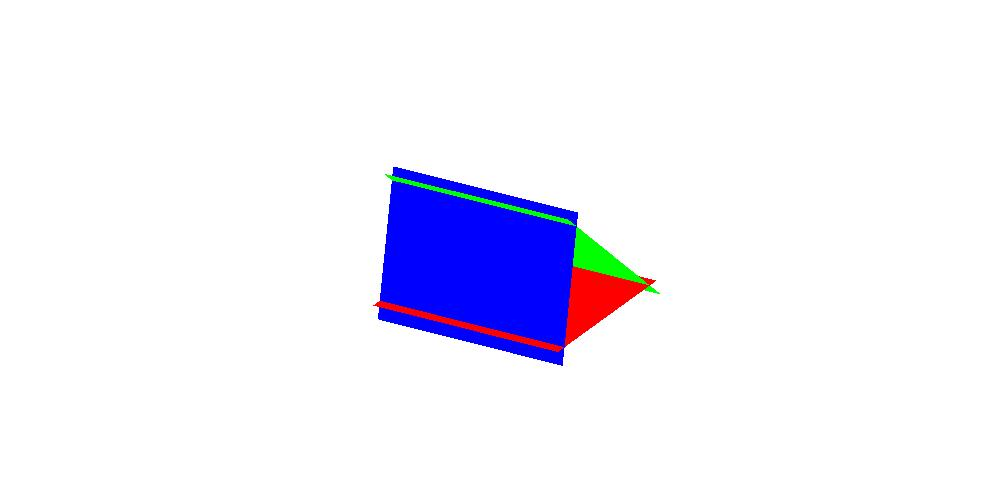
\includegraphics[scale=0.5,clip=true,
      trim=10cm 4.5cm 10cm 5.5cm]{images/toblerone}
 \]

\end{example}

\begin{example}\label{eg-lineq-ii}
 We will solve the equations
 \begin{align*}
  a + b + c + d &= 4 \\
  a + b - c - d &= 0 \\
  a - b + c - d &= 0 \\
  a - b - c + d &= 0.
 \end{align*}
 The corresponding augmented matrix can be row-reduced as follows:
 \[
  \left[\begin{array}{cccc|c}
    1 &  1 &  1 &  1 & 4 \\
    1 &  1 & -1 & -1 & 0 \\
    1 & -1 &  1 & -1 & 0 \\
    1 & -1 & -1 &  1 & 0
  \end{array}\right]
  \xra{1}
  \left[\begin{array}{cccc|c}
    1 &  1 &  1 &  1 &  4 \\
    0 &  0 & -2 & -2 & -4 \\
    1 & -1 &  1 & -1 & 0 \\
    0 &  0 & -2 &  2 & 0
  \end{array}\right]
  \xra{2}
  \left[\begin{array}{cccc|c}
    1 &  1 &  1 &  1 &  4 \\
    0 &  0 &  1 &  1 &  2 \\
    1 & -1 &  1 & -1 & 0 \\
    0 &  0 &  1 & -1 & 0
  \end{array}\right]
  \xra{3}
 \] \[
  \left[\begin{array}{cccc|c}
    1 &  1 &  0 &  0 & 2 \\
    0 &  0 &  1 &  1 & 2 \\
    1 & -1 &  0 &  0 & 0 \\
    0 &  0 &  1 & -1 & 0
  \end{array}\right]
  \xra{4}
  \left[\begin{array}{cccc|c}
    1 &  1 &  0 &  0 & 2 \\
    0 &  0 &  1 &  1 & 2 \\
    0 & -2 &  0 &  0 & -2 \\
    0 &  0 &  0 & -2 & -2
  \end{array}\right]
  \xra{5}
  \left[\begin{array}{cccc|c}
    1 &  1 &  0 &  0 & 2 \\
    0 &  0 &  1 &  1 & 2 \\
    0 &  1 &  0 &  0 & 1 \\
    0 &  0 &  0 &  1 & 1
  \end{array}\right]
  \xra{6}
 \] \[
  \left[\begin{array}{cccc|c}
    1 &  0 &  0 &  0 & 1 \\
    0 &  0 &  1 &  0 & 1 \\
    0 &  1 &  0 &  0 & 1 \\
    0 &  0 &  0 &  1 & 1
  \end{array}\right]
  \xra{7}
  \left[\begin{array}{cccc|c}
    1 &  0 &  0 &  0 & 1 \\
    0 &  1 &  0 &  0 & 1 \\
    0 &  0 &  1 &  0 & 1 \\
    0 &  0 &  0 &  1 & 1
  \end{array}\right]
 \]
 Here, rather than slavishly following Method~\ref{meth-RREF}, we have
 applied row operations in a more creative order to make the structure
 of the equations clearer.  The stages are as follows:
 \begin{itemize}
  \item[1] We subtract the first row from the second, and the third
   from the fourth.
  \item[2] We multiply the second and fourth rows by $-1/2$.
  \item[3] We subtract the second row from the first, and the fourth
   from the third.
  \item[4] We subtract the first row from the third, and the second
   from the fourth.
  \item[5] We multiply the third and fourth rows by $-1/2$.
  \item[6] We subtract the third row from the first, and the fourth
   from the second.
  \item[7] We exchange the second and third rows.
 \end{itemize}
 The final matrix corresponds to the equations $a=1$, $b=1$, $c=1$ and
 $d=1$, which give the unique solution to the original system of
 equations.
\end{example}

\begin{remark}
 Often we want to solve a \dfn{homogeneous} equation $Ax=0$, where
 the right hand side is zero.  This means that the relevant augmented
 matrix is $[A|0]$.  Row operations will not change the fact that the last
 column is zero, so the RREF of $[A|0]$ will just be $[A'|0]$, where
 $A'$ is the RREF of $A$.  In this context we can save writing by
 leaving out the extra column and just working with $A$.
\end{remark}
\begin{example}\label{eg-homogeneous}
 Consider the homogeneous system
 \begin{align*}
  a+b+c+d+e+f &= 0 \\
  2a+2b+2c+2d-e-f &= 0 \\
  3a+3b-c-d-e-f &= 0
 \end{align*}
 The corresponding unaugmented matrix can be row-reduced as follows:
 \[
  \bbm
    1 &  1 &  1 &  1 &  1 &  1 \\
    2 &  2 &  2 &  2 & -1 & -1 \\
    3 &  3 & -1 & -1 & -1 & -1
  \ebm \to \bbm
    1 &  1 &  0 &  0 &  0 &  0 \\
    0 &  0 &  1 &  1 &  0 &  0 \\
    0 &  0 &  0 &  0 &  1 &  1 
  \ebm
 \]
 (details are left to the reader).  The final matrix corresponds to
 the homogeneous system
 \[ a+b = 0 \hspace{5em} c+d=0 \hspace{5em} e+f=0. \]
 There are pivots in columns $1$, $3$ and $5$, meaning that $a$, $c$
 and $e$ are dependent variables, and $b$, $d$ and $f$ are
 independent.  After moving the independent variables to the right
 hand side, the solution becomes $a=-b$, $c=-d$ and $e=-f$.  If we
 prefer we can introduce new variables $\lm$, $\mu$ and $\nu$, and say
 that the general solution is
 \begin{align*}
  a &= -\lm & c &= -\mu & e &= -\nu \\
  b &=  \lm & d &=  \mu & f &=  \nu
 \end{align*}
 for arbitrary values of $\lm$, $\mu$ and $\nu$.
\end{example}

\section{Linear combinations}
\label{sec-lin-comb}

\begin{definition}\label{defn-lincomb}
 Let $v_1,\dotsc,v_k$ and $w$ be vectors in $\R^n$.  We say that $w$
 is a \dfn{linear combination} of $v_1,\dotsc,v_k$ if there exist
 scalars $\lm_1,\dots,\lm_k$ such that
 \[ w = \lm_1v_1 + \dotsb + \lm_kv_k. \]
 
 In the same way, the notion of a linear combination is defined
 for row vectors instead of columns.
 (But it offers nothing new, since a row vector $w$ is a
 linear combination of $k$ row vectors $v_1,\dotsc,v_k$
 if and only if its transpose $w^T$ is a linear combination
 of $v_1^T,\dotsc,v_k^T$.)
\end{definition}

\begin{example}\label{eg-lincomb-i}
 Consider the following vectors in $\R^4$:
 \[ v_1 = \bbm 1 \\ -1 \\ 0 \\ 0 \ebm \hspace{3em}
    v_2 = \bbm 0 \\ 1 \\ -1 \\ 0 \ebm \hspace{3em}
    v_3 = \bbm 0 \\ 0 \\ 1 \\ -1 \ebm \hspace{3em}
    w   = \bbm 1 \\ 10 \\ 100 \\ -111 \ebm
 \]
 If we take $\lm_1=1$ and $\lm_2=11$ and $\lm_3=111$ we get
 \[ \lm_1 v_1 + \lm_2 v_2 + \lm_3 v_3 =
     \bbm 1 \\ -1 \\ 0 \\ 0 \ebm +
     \bbm 0 \\ 11 \\ -11 \\ 0 \ebm +
     \bbm 0 \\ 0 \\ 111 \\ -111 \ebm =
     \bbm 1 \\ 10 \\ 100 \\ -111 \ebm = w,
 \]
 which shows that $w$ is a linear combination of $v_1$, $v_2$ and
 $v_3$.
\end{example}

\begin{example}\label{eg-lincomb-ii}
 Consider the following vectors in $\R^4$:
 \[ v_1 = \bbm 0 \\ 1 \\  2 \\  3 \ebm \hspace{3em}
    v_2 = \bbm 0 \\ 1 \\  4 \\  9 \ebm \hspace{3em}
    v_3 = \bbm 0 \\ 1 \\  8 \\ 27 \ebm \hspace{3em}
    v_4 = \bbm 0 \\ 1 \\ 16 \\ 81 \ebm \hspace{3em}
    w = \bbm 1 \\ 1 \\ 1 \\ 1 \ebm.
 \]
 Any linear combination of $v_1,\dotsc,v_4$ has the form
 \[ \lm_1v_1 + \lm_2v_2 + \lm_3v_3 + \lm_4v_4 =
     \bbm 0 \\ \lm_1+\lm_2+\lm_3+\lm_4 \\
          2\lm_1+4\lm_2+8\lm_3+16\lm_4 \\
          3\lm_1+9\lm_2+27\lm_3+81\lm_4 \ebm.
 \]
 In particular, the first component of any such linear combination is
 zero.  (You should be able to see this without needing to write out
 the whole formula.)  As the first component of $w$ is not zero, we
 see that $w$ is \emph{not} a linear combination of $v_1,\dotsc,v_4$.
\end{example}

\begin{example}\label{eg-lincomb-iii}
 Consider the following vectors in $\R^3$:
 \[ v_1 = \bbm 1 \\ 1 \\ 1 \ebm \hspace{3em}
    v_2 = \bbm 1 \\ 2 \\ 1 \ebm \hspace{3em}
    v_3 = \bbm 1 \\ 3 \\ 1 \ebm \hspace{3em}
    v_4 = \bbm 1 \\ 4 \\ 1 \ebm \hspace{3em}
    v_5 = \bbm 1 \\ 5 \\ 1 \ebm \hspace{3em}
    w   = \bbm -1 \\ 0 \\ 1 \ebm.
 \]
 Any linear combination of $v_1,\dotsc,v_5$ has the form
 \[ \lm_1v_1 + \dotsb + \lm_5v_5 =
     \bbm \lm_1+\lm_2+\lm_3+\lm_4+\lm_5 \\
          \lm_1+2\lm_2+3\lm_3+4\lm_4+5\lm_5 \\
          \lm_1+\lm_2+\lm_3+\lm_4+\lm_5 \ebm.
 \]
 In particular, the first and last components of any such linear
 combination are the same.  Again, you should be able to see this
 without writing the full formula.  As the first and last components
 of $w$ are different, we see that $w$ is not a linear combination of
 $v_1,\dotsc,v_5$.
\end{example}
\begin{example}\label{eg-lincomb-iv}
 Let $v_1$, $v_2$ and $w$ be vectors in $\R^3$ (so we can think about
 them geometrically).  For simplicity, assume that all three vectors
 are nonzero, and that $v_1$ and $v_2$ do not point in the same
 direction, nor do they point in opposite directions.  This will mean
 that there is a unique plane $P$ that passes through $v_1$, $v_2$ and
 the origin.  It is not hard to see that $P$ is just the set of all
 possible linear combinations of $v_1$ and $v_2$.  Thus, our vector
 $w$ is a linear combination of $v_1$ and $v_2$ if and only if $w$
 lies in the plane $P$.
 \[ 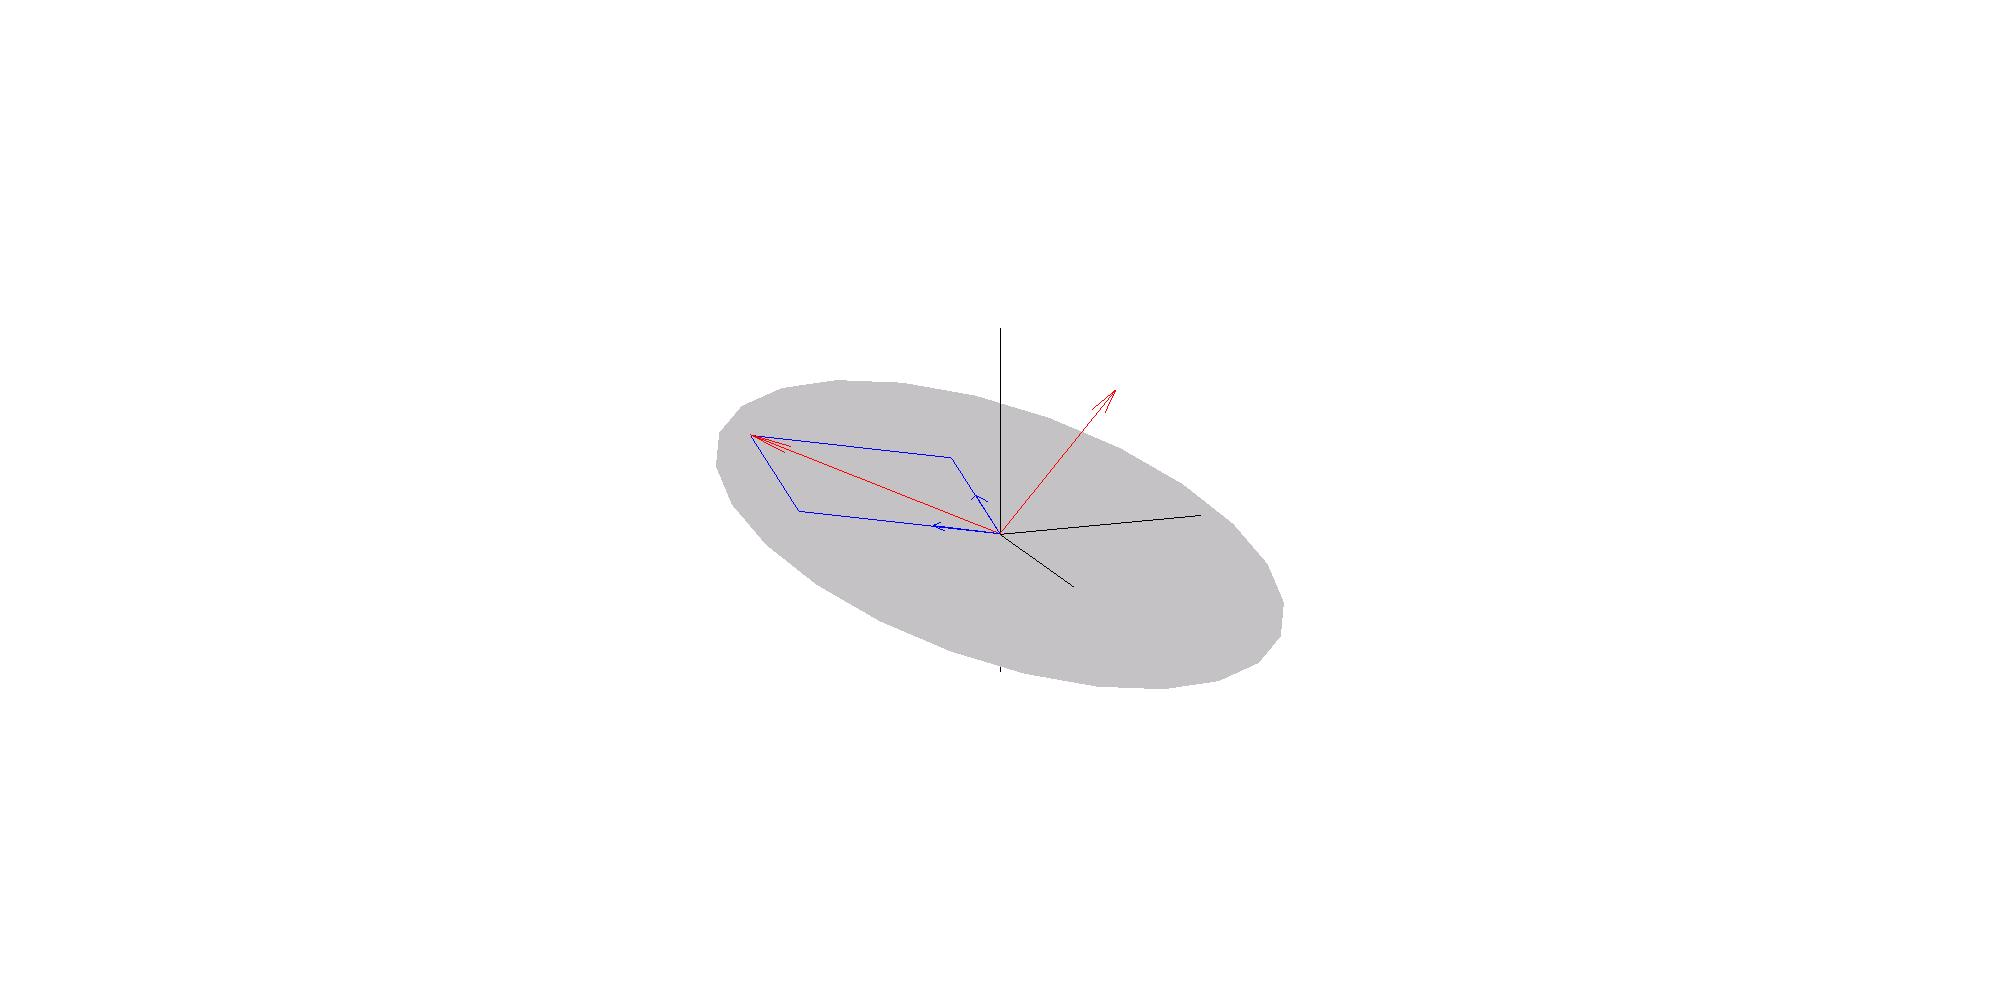
\includegraphics[scale=0.4,clip=true,
      trim=20cm 9cm 20cm 11cm]{images/plane_span}
 \]
\end{example}

We now want to explain a more systematic way to check whether a given
vector is a linear combination of some given list of vectors.
Note that for any $k$-vector
$\lm=\bbm\lm_1 & \dotsb & \lm_k\ebm^T$ we have
\[ A\lm =
    \left[\begin{array}{c|c|c}
     v_1 & \cdots & v_k
    \end{array}\right]
    \bbm \lm_1 \\ \vdots \\ \lm_k \ebm =
    \lm_1 v_1 + \dotsb + \lm_k v_k,
\]
which is the general form for a linear combination of
$v_1,\dotsc,v_k$.  This makes it clear that $w$ is a linear
combination of $v_1,\dotsc,v_k$ if and only if there is a vector $\lm$
which solves the matrix equation $A\lm=w$.  Using
Theorem~\ref{thm-row-ops} we see that the equation $A\lm=w$ has the
same solutions as the equation $A'\lm=w'$, which can be solved easily
by Method~\ref{meth-RREF-solve}.  We thus arrive at the following
method: 

\begin{method}\label{meth-find-lincomb}
 \index{linear combination}
 Suppose we have vectors $v_1,\dotsc,v_k\in\R^n$ and another vector
 $w\in\R^n$, and we want to express $w$ as a linear combination of the
 $v_i$ (or show that this is not possible).
 \begin{itemize}
  \item[(a)] We first let $A$ be the matrix whose columns are the
   vectors $v_i$:
   \[ A = \left[\begin{array}{c|c|c}
       v_1 & \cdots & v_k
      \end{array}\right] \in M_{n\tm k}(\R).
   \]
  \item[(b)] We then append $w$ as an additional column to get an
   augmented matrix
   \[ B  = \left[\begin{array}{c|c|c|c}
       v_1 & \cdots & v_k & w
      \end{array}\right]
       = \left[\begin{array}{c|c} A & w\end{array}\right].
   \]
   This corresponds to the matrix equation $A\lm=w$.
  \item[(c)] Row-reduce $B$ by Method~\ref{meth-RREF} to get a matrix
   $B'=[A'|w']$ in RREF.
  \item[(d)] If $B'$ has a pivot in the last column, then $w$ is not a
   linear combination of the vectors $v_1,\dotsc,v_k$.
  \item[(e)] If $B'$ has no pivot in the last column, then we can use
   Method~\ref{meth-RREF-solve} to find a vector
   $\lm=\bbm\lm_1 & \cdots & \lm_k\ebm^T$ satisfying $A'\lm=w'$.  We
   then have $A\lm=w$ and $\lm_1v_1+\dotsb+\lm_kv_k=w$, showing that
   $w$ is a linear combination of $v_1,\dotsc,v_k$.
 \end{itemize}
\end{method}

\begin{example}\label{eg-find-lincomb-i}
 Consider the vectors
 \[ v_1 = \bbm 11 \\ 11 \\ 1 \\ 1 \ebm \hspace{3em}
    v_2 = \bbm 1 \\ 11 \\ 11 \\ 1 \ebm \hspace{3em}
    v_3 = \bbm 1 \\ 1 \\ 11 \\ 11 \ebm \hspace{3em}
    w   = \bbm 121 \\ 221 \\ 1211 \\ 1111 \ebm.
 \]
 We ask whether $w$ can be expressed as a linear combination
 $w=\lm_1v_1+\lm_2v_2+\lm_3v_3$, and if so, what are the relevant
 values $\lm_1$, $\lm_2$ and $\lm_3$?  Following
 Method~\ref{meth-find-lincomb}, we write down the augmented
 matrix $[v_1|v_2|v_3|w]$ and row-reduce it:
 \[
  \left[\begin{array}{ccc|c}
   11 &  1 &  1 & 121 \\
   11 & 11 &  1 & 221 \\
    1 & 11 & 11 & 1211 \\
    1 &  1 & 11 & 1111
  \end{array}\right]
  \xra{1}
  \left[\begin{array}{ccc|c}
    1 &  1 & 11 & 1111 \\
   11 &  1 &  1 & 121 \\
   11 & 11 &  1 & 221 \\
    1 & 11 & 11 & 1211
  \end{array}\right]
  \xra{2}
  \left[\begin{array}{ccc|c}
    1 &   1 &   11 & 1111 \\
    0 & -10 & -120 & -12100 \\
    0 &   0 & -120 & -12000 \\
    0 &  10 &    0 & 100
  \end{array}\right]
  \xra{3}
 \] \[
  \left[\begin{array}{ccc|c}
    1 &   1 &   11 & 1111 \\
    0 &   1 &   12 & 1210 \\
    0 &   0 &    1 & 100 \\
    0 &   1 &    0 & 10
  \end{array}\right]
  \xra{4}
  \left[\begin{array}{ccc|c}
    1 &   1 &    0 & 11 \\
    0 &   1 &    0 & 10 \\
    0 &   0 &    1 & 100 \\
    0 &   1 &    0 & 10
  \end{array}\right]
  \xra{5}
  \left[\begin{array}{ccc|c}
    1 &   0 &    0 & 1 \\
    0 &   1 &    0 & 10 \\
    0 &   0 &    1 & 100 \\
    0 &   0 &    0 & 0
  \end{array}\right]
 \]
 (1: move the bottom row to the top; 2: subtract multiples of row 1
 from the other rows; 3: divide rows 2,3 and 4 by $-10$, $-120$ and
 $10$; 4: subtract multiples of row 3 from the other rows; 5: subtract
 multiples of row 2 from the other rows.)

 The final matrix corresponds to the system of equations
 \[ \lm_1 = 1 \hspace{3em}
    \lm_2 = 10 \hspace{3em}
    \lm_3 = 100 \hspace{3em}
     0 = 0
 \]
 so we conclude that
 \[ w = v_1 + 10 v_2 + 100 v_3. \]
 In particular, $w$ can be expressed as a linear combination of $v_1$,
 $v_2$ and $v_3$.  We can check the above equation directly:
 \[ v_1 + 10 v_2 + 100 v_3 =
      \bbm  11 \\  11 \\    1 \\    1 \ebm +
      \bbm  10 \\ 110 \\  110 \\   10 \ebm +
      \bbm 100 \\ 100 \\ 1100 \\ 1100 \ebm
    = \bbm 121 \\ 221 \\ 1211 \\ 1111 \ebm = w.
 \]
\end{example}

\begin{example}\label{eg-find-lincomb-ii}
 Consider the vectors
 \[ a_1 = \bbm 2 \\ -1 \\  0 \ebm \hspace{3em}
    a_2 = \bbm 3 \\  0 \\ -1 \ebm \hspace{3em}
    a_3 = \bbm 0 \\  3 \\ -2 \ebm \hspace{3em}
    b = \bbm 1 \\ 2 \\ 3 \ebm
 \]
 To test whether $b$ is a linear combination of $a_1$, $a_2$ and
 $a_3$, we write down the relevant augmented matrix and row-reduce it:
 \[
  \left[\begin{array}{ccc|c}
    2 &  3 &  0 & 1 \\
   -1 &  0 &  3 & 2 \\
    0 & -1 & -2 & 3
  \end{array}\right]
  \xra{1}
  \left[\begin{array}{ccc|c}
    1 &  0 & -3 & -2 \\
    0 &  1 &  2 & -3 \\
    2 &  3 &  0 &  1
  \end{array}\right]
  \xra{2}
  \left[\begin{array}{ccc|c}
    1 &  0 & -3 & -2 \\
    0 &  1 &  2 & -3 \\
    0 &  3 &  6 &  5
  \end{array}\right]
  \xra{3}
 \] \[
  \left[\begin{array}{ccc|c}
    1 &  0 & -3 & -2 \\
    0 &  1 &  2 & -3 \\
    0 &  0 &  0 & 14
  \end{array}\right]
  \xra{4}
  \left[\begin{array}{ccc|c}
    1 &  0 & -3 & -2 \\
    0 &  1 &  2 & -3 \\
    0 &  0 &  0 &  1
  \end{array}\right]
  \xra{5}
  \left[\begin{array}{ccc|c}
    1 &  0 & -3 &  0 \\
    0 &  1 &  2 &  0 \\
    0 &  0 &  0 &  1
  \end{array}\right]
 \]
 (Stage 1: move the top row to the bottom, and multiply the other two rows
 by $-1$; Stage 2: subtract $2$ times row 1 from row 3; Stage 3:
 subtract $3$ times row 2 from row 3; Stage 4: divide row 3 by $14$;
 Stage 5: subtract multiples of row 3 from rows 1 and 2.)

 The last matrix has a pivot in the rightmost column, corresponding to
 the equation $0=1$.  This means that the equation
 $\lm_1a_1+\lm_2a_2+\lm_3a_3=b$ cannot be solved for $\lm_1$, $\lm_2$
 and $\lm_3$, or in other words that $b$ is not a linear combination
 of $a_1$, $a_2$ and $a_3$.

 We can also see this in a more direct but less systematic way, as
 follows.  It is easy to check that $b.a_1=b.a_2=b.a_3=0$, which means
 that $b.(\lm_1a_1+\lm_2a_2+\lm_3a_3)=0$ for all possible choices of
 $\lm_1$, $\lm_2$ and $\lm_3$.  However, $b.b=14>0$, so $b$ cannot be
 equal to $\lm_1a_1+\lm_2a_2+\lm_3a_3$.
\end{example}

\section{Linear independence}

\begin{definition}\label{defn-dependent}
 Let $\CV=v_1,\dotsc,v_k$ be a list of vectors in $\R^n$.  A
 \dfn{linear relation} between the vectors $v_i$ is a relation of the
 form $\lm_1v_1+\dotsb+\lm_kv_k=0$, where $\lm_1,\dotsc,\lm_k$ are
 scalars.  In other words, it is a way of expressing $0$ as a linear
 combination of $\CV$.

 For any list we have the trivial linear relation
 $0v_1+0v_2+\dotsb+0v_k=0$.  There may or may not be any nontrivial
 linear relations.

 If the list $\CV$ has a nontrivial linear relation, we say that it is
 a \dfn{linearly dependent} list.  If the only linear relation on
 $\CV$ is the trivial one, we instead say that $\CV$ is \dfn{linearly
  independent}.  We will often omit the word ``linearly'' for the sake
 of brevity.
 
 All this language is defined in the same way for row vectors
 instead of column vectors.
\end{definition}

\begin{example}\label{eg-dep-i}
 Consider the list $\CV$ given by
 \[ v_1 = \bbm 1 \\ 1 \\ 0 \\ 0 \ebm \hspace{3em}
    v_2 = \bbm 0 \\ 0 \\ 1 \\ 1 \ebm \hspace{3em}
    v_3 = \bbm 1 \\ 0 \\ 0 \\ 1 \ebm \hspace{3em}
    v_4 = \bbm 0 \\ 1 \\ 1 \\ 0 \ebm.
 \]
 There is a nontrivial linear relation $v_1+v_2-v_3-v_4=0$, so the
 list $\CV$ is dependent.
\end{example}
\begin{example}\label{eg-dep-ii}
\begin{itemize}
 \item[(a)]
 Consider the list $\CA$ given by
 \[ a_1 = \bbm  1 \\  2 \ebm \hspace{3em}
    a_2 = \bbm 12 \\  1 \ebm \hspace{3em}
    a_3 = \bbm -1 \\ -1 \ebm \hspace{3em}
    a_4 = \bbm  3 \\  1 \ebm.
 \]
 Just by writing it out, you can check that
 \[ 3a_1 + a_2 + 3a_3 -4a_4 = 0. \]
 \begin{center}
  \begin{tikzpicture}[scale=0.3]
   \fill( 0,0) circle(0.1);
   \fill( 3,6) circle(0.1);
   \fill(15,7) circle(0.1);
   \fill(12,4) circle(0.1);
   \draw[->, shorten >= 1pt] (0,0) -- (3,6);
   \draw[->, shorten >= 1pt] (3,6) -- (15,7);
   \draw[->, shorten >= 1pt] (15,7) -- (12,4);
   \draw[->, shorten >= 1pt] (12,4) -- (0,0);
   \draw ( 1.5,3.0) node[anchor=south east]{$\scriptstyle 3a_1$};
   \draw ( 9.0,6.5) node[anchor=south]{$\scriptstyle a_2$};
   \draw (13.5,5.5) node[anchor=north west]{$\scriptstyle 3a_3$};
   \draw ( 6.0,2.0) node[anchor=north]{$\scriptstyle -4a_4$};
  \end{tikzpicture}
 \end{center}
 This is a nontrivial linear relation on the list $\CA$, so $\CA$ is
 dependent.
 
 \item[(b)]
 Consider the list $\CB$ given by
 \[
    b_1 = \begin{bmatrix} 1 \\ 0 \end{bmatrix} \hspace{3em}
    b_2 = \begin{bmatrix} 2 \\ 0 \end{bmatrix} \hspace{3em}
    b_3 = \begin{bmatrix} 0 \\ 1 \end{bmatrix} .
 \]
 This list $\CB$, too, is dependent, since
 $2 b_1 - 1 b_2 + 0 b_3 = 0$.
 (This shows that even the smaller list $\left( b_1, b_2 \right)$
 is dependent.)
\end{itemize}
\end{example}
\begin{example}\label{eg-indep-i}
 Consider the list $\CU$ given by
 \[ u_1 = \bbm 1 \\ 1 \\ 0 \\ 0 \ebm \hspace{3em}
    u_2 = \bbm 0 \\ 1 \\ 1 \\ 0 \ebm \hspace{3em}
    u_3 = \bbm 0 \\ 0 \\ 1 \\ 1 \ebm.
 \]
 We claim that this is independent.  To see this, consider a linear
 relation $\lm_1u_1+\lm_2u_2+\lm_3u_3=0$.  Writing this out, we get
 \[ \bbm \lm_1 \\ \lm_1+\lm_2 \\ \lm_2+\lm_3 \\ \lm_3 \ebm =
    \bbm 0 \\ 0 \\ 0 \\ 0 \ebm.
 \]
 By looking at the first and last rows we see that $\lm_1=\lm_3=0$.
 By looking at the second row we get $\lm_2=-\lm_1=0$ as well so our
 relation is the trivial relation.  As the only linear relation is the
 trivial one, we see that $\CU$ is independent.
\end{example}

\begin{lemma}\label{lem-multiples}
 Let $v$ and $w$ be vectors in $\R^n$, and suppose that $v\neq 0$ and
 that the list $(v,w)$ is linearly dependent.  Then there is a number
 $\al$ such that $w=\al v$.
\end{lemma}
\begin{proof}
 Because the list is dependent, there is a linear relation
 $\lm v+\mu w=0$ where $\lm$ and $\mu$ are not both zero.  There are
 apparently three possibilities: (a) $\lm\neq 0$ and $\mu\neq 0$; (b)
 $\lm=0$ and $\mu\neq 0$; (c) $\lm\neq 0$ and $\mu=0$.  However,
 case~(c) is not really possible.  Indeed, in case~(c) the equation
 $\lm v+\mu w=0$ would reduce to $\lm v=0$, and we could multiply by
 $\lm^{-1}$ to get $v=0$; but $v\neq 0$ by assumption.  In case~(a)
 or~(b) we can take $\al=-\lm/\mu$ and we have $w=\al v$.
\end{proof}

There is a systematic method using row-reduction for checking linear
(in)dependence, as we will explain shortly.  We first need a
preparatory observation.

\begin{definition}\label{defn-wide}
 Let $B$ be a $p\tm q$ matrix.  We say that $B$ is \dfn{wide} if
 $p<q$, or \dfn{square} if $p=q$, or \dfn{tall} if $p>q$.
 \[ \begin{array}{ccccc}
     \bbm 1 & 2 & 3 \\ 4 & 5 & 6 \ebm & &
     \bbm 1 & 2 & 1 \\ 2 & 3 & 2 \\ 1 & 2 & 1 \ebm & &
     \bbm 1 & 1 \\ 0 & 0 \\ 1 & 1 \ebm \\
     \text{ wide } & & \text{ square } & & \text{ tall }
    \end{array}
 \]
\end{definition}
\begin{lemma}\label{lem-pivots-everywhere}
 \index{pivot}
 Let $B$ be a $p\tm q$ matrix in RREF.
 \begin{itemize}
  \item[(a)] If $B$ is wide then it is impossible for every column to
   contain a pivot.
  \item[(b)] If $B$ is square then the only way for every column to
   contain a pivot is if $B=I_q$.
  \item[(c)] If $B$ is tall  then the only way for every column to
   contain a pivot is if $B$ consists of $I_q$ with $(p-q)$ rows of
   zeros added at the bottom (so
   $B=\left[\begin{array}{c} I_q \\ \hline 0_{(p-q)\tm q}
      \end{array}\right]$).
 \end{itemize}
\end{lemma}

For example, the only $5\tm 3$ RREF matrix with a pivot in every
column is this one:
\[ \left[\begin{array}{c}
      I_3 \\ \hline 0_{2\tm 3} 
   \end{array}\right] =
   \left[\begin{array}{ccc}
    1 & 0 & 0 \\
    0 & 1 & 0 \\
    0 & 0 & 1 \\ \hline
    0 & 0 & 0 \\
    0 & 0 & 0
   \end{array}\right]
\]

\begin{proof}
 There is at most one pivot in every row, making at most $p$ pivots
 altogether.  If $B$ is wide then we have $q$ columns with $q>p$, so
 there are not enough pivots to have one in every column.  This
 proves~(a).

 Now suppose instead that $B$ does have a pivot in every column, so
 there are $q$ pivots and we must have $p\geq q$.  As $B$ is in RREF
 we know that all entries above or below a pivot are zero.  As there
 is a pivot in every column it follows that the pivots are the only
 nonzero entries in $B$.  Every nonzero row contains precisely one
 pivot, so there must be $q$ nonzero rows.  The remaining $(p-q)$ rows
 are all zero, and they must occur at the bottom of $B$ (because $B$
 is in RREF).  Now the top $q\tm q$ block contains $q$ pivots which
 move to the right as we go down the matrix.  It is easy to see that
 the only possibility for the top block is $I_q$, which proves~(b)
 and~(c).
\end{proof}

\begin{method}\label{meth-check-dependence}
 \index{linearly dependent}\index{linearly independent}\index{pivot}
 Let $\CV=v_1,\dotsc,v_m$ be a list of vectors in $\R^n$.  We can
 check whether this list is dependent as follows.
 \begin{itemize}
  \item[(a)] Form the $n\tm m$ matrix
   \[ A = \left[\begin{array}{c|c|c}
              && \\
              v_1 & \dotsc & v_m \\
              &&
            \end{array}\right]
   \]
   whose columns are the vectors $v_i$.
  \item[(b)] Row reduce $A$ to get another $n\tm m$ matrix $B$ in
   RREF.
  \item[(c)] If every column of $B$ contains a pivot (so $B$ has the
   form discussed in Lemma~\ref{lem-pivots-everywhere}) then $\CV$ is
   independent.
  \item[(d)] If some column of $B$ has no pivot, then the list $\CV$
   is dependent.  Moreover, we can find the coefficients $\lm_i$ in a
   nontrivial linear relation by solving the vector equation $B\lm=0$
   (which is easy because $B$ is in RREF).
 \end{itemize}
\end{method}
\begin{remark}\label{rem-dependence-shortcut}
 \index{wide}\index{numerical criteria}
 If $m>n$ then $\CV$ is automatically dependent and we do not need to
 go through the method.  (For example, any list of $5$ vectors in
 $\R^3$ is automatically dependent, any list of $10$ vectors in $\R^9$
 is automatically dependent, and so on.)  Indeed, in this case the
 matrices $A$ and $B$ are wide, so it is impossible for $B$ to have a
 pivot in every column.  However, this line of argument only tells us
 that there \textbf{exists} a nontrivial relation
 $\lm_1v_1+\dotsb+\lm_mv_m=0$, it does not tell us the coefficients
 $\lm_i$.  If we want to find the $\lm_i$ then we do need to go
 through the whole method as explained above.
\end{remark}

We will give some examples of using the above method, and then explain
why the method is correct.

\begin{example}\label{eg-dep-i-matrix}
 In example~\ref{eg-dep-i} we considered the list
 \[ v_1 = \bbm 1 \\ 1 \\ 0 \\ 0 \ebm \hspace{3em}
    v_2 = \bbm 0 \\ 0 \\ 1 \\ 1 \ebm \hspace{3em}
    v_3 = \bbm 1 \\ 0 \\ 0 \\ 1 \ebm \hspace{3em}
    v_4 = \bbm 0 \\ 1 \\ 1 \\ 0 \ebm.
 \]
 We can write down the corresponding matrix and row-reduce it as
 follows:
 \[
  \bbm 1 & 0 & 1 & 0 \\
       1 & 0 & 0 & 1 \\
       0 & 1 & 0 & 1 \\
       0 & 1 & 1 & 0
  \ebm \xra{1}
  \bbm 1 & 0 & 1 & 0 \\
       0 & 0 &-1 & 1 \\
       0 & 1 & 0 & 1 \\
       0 & 0 & 1 &-1
  \ebm \xra{2}
  \bbm 1 & 0 & 1 & 0 \\
       0 & 1 & 0 & 1 \\
       0 & 0 & 1 &-1 \\
       0 & 0 &-1 & 1
  \ebm \xra{3}
  \bbm 1 & 0 & 0 & 1 \\
       0 & 1 & 0 & 1 \\
       0 & 0 & 1 &-1 \\
       0 & 0 & 0 & 0
  \ebm
 \]
 The end result has no pivot in the last column, so the original list is
 dependent.  To find a specific linear relation, we solve the equation
 \[   \bbm 1 & 0 & 0 & 1 \\
           0 & 1 & 0 & 1 \\
           0 & 0 & 1 &-1 \\
           0 & 0 & 0 & 0
      \ebm
      \bbm \lm_1 \\ \lm_2 \\ \lm_3 \\ \lm_4 \ebm =
      \bbm 0 \\ 0 \\ 0 \\ 0 \ebm
 \]
 to get $\lm_1=-\lm_4$, $\lm_2=-\lm_4$ and $\lm_3=\lm_4$ with $\lm_4$
 arbitrary.  Taking $\lm_4=1$ gives
 $(\lm_1,\lm_2,\lm_3,\lm_4)=(-1,-1,1,1)$, corresponding to the
 relation $-v_1-v_2+v_3+v_4=0$.
\end{example}
\begin{example}\label{eg-dep-ii-matrix}
 In Example~\ref{eg-dep-ii} (a) we considered the list
 \[ a_1 = \bbm  1 \\  2 \ebm \hspace{3em}
    a_2 = \bbm 12 \\  1 \ebm \hspace{3em}
    a_3 = \bbm -1 \\ -1 \ebm \hspace{3em}
    a_4 = \bbm  3 \\  1 \ebm.
 \]
 Here we have $4$ vectors in $\R^2$, so they must be dependent by
 Remark~\ref{rem-dependence-shortcut}.  Thus, there exist nontrivial
 linear relations
 \[ \lm_1a_1 + \lm_2a_2 + \lm_3a_3 + \lm_4a_4 = 0. \]
 To actually find such a relation, we write down the corresponding
 matrix and row-reduce it as follows:
 \[
  \bbm
   1 & 12 & -1 & 3 \\
   2 & 1  & -1 & 1
  \ebm
  \xra{}
  \bbm
   1 &  12 & -1 & 3 \\
   0 & -23 &  1 & -5
  \ebm
  \xra{}
  \bbm
   1 &  12 & -1 & 3 \\
   0 &  1 & -1/23 & 5/23
  \ebm
  \xra{}
  \bbm
   1 &  0 & -11/23 & 9/23 \\
   0 &  1 & -1/23 & 5/23
  \ebm
 \]
 We now need to solve the matrix equation
 \[ \bbm
     1 &  0 & -11/23 & 9/23 \\
     0 &  1 & -1/23 & 5/23
    \ebm
    \bbm \lm_1 \\ \lm_2 \\ \lm_3 \\ \lm_4 \ebm =
    \bbm 0 \\ 0 \ebm
 \]
 As this is in RREF, we can just read off the solution:
 $\lm_1=\frac{11}{23}\lm_3-\frac{9}{23}\lm_4$ and
 $\lm_2=\frac{1}{23}\lm_3-\frac{5}{23}\lm_4$
 with $\lm_3$ and $\lm_4$ arbitrary.  If we choose $\lm_3=23$ and
 $\lm_4=0$ we get $(\lm_1,\lm_2,\lm_3,\lm_4)=(11,1,23,0)$ so we have a
 relation
 \[ 11 a_1 + a_2 + 23 a_3 + 0 a_4 = 0. \]
 (You should check directly that this is correct.)  Alternatively, we
 can choose $\lm_3=3$ and $\lm_4=-4$.  Using the equations
 $\lm_1=\frac{11}{23}\lm_3-\frac{9}{23}\lm_4$ and
 $\lm_2=\frac{1}{23}\lm_3-\frac{5}{23}\lm_4$ we get $\lm_1=3$ and
 $\lm_2=1$ giving a different relation
 \[ 3a_1 + a_2 + 3a_3 - 4a_4 = 0. \]
 This is the relation that we observed in Example~\ref{eg-dep-ii} (a).
\end{example}
\begin{example}\label{eg-indep-i-matrix}
 In Example~\ref{eg-indep-i} we considered the list $\CU$ given by
 \[ u_1 = \bbm 1 \\ 1 \\ 0 \\ 0 \ebm \hspace{3em}
    u_2 = \bbm 0 \\ 1 \\ 1 \\ 0 \ebm \hspace{3em}
    u_3 = \bbm 0 \\ 0 \\ 1 \\ 1 \ebm.
 \]
 We can write down the corresponding matrix and row-reduce it as
 follows:
 \[
  \bbm
   1 & 0 & 0 \\
   1 & 1 & 0 \\
   0 & 1 & 1 \\
   0 & 0 & 1
  \ebm
  \to
  \bbm
   1 & 0 & 0 \\
   0 & 1 & 0 \\
   0 & 1 & 1 \\
   0 & 0 & 1
  \ebm
  \to
  \bbm
   1 & 0 & 0 \\
   0 & 1 & 0 \\
   0 & 0 & 1 \\
   0 & 0 & 1
  \ebm
  \to
  \left[\begin{array}{ccc}
   1 & 0 & 0 \\
   0 & 1 & 0 \\
   0 & 0 & 1 \\ \hline
   0 & 0 & 0
  \end{array}\right]
 \]
 The final matrix has a pivot in every column, as in
 Lemma~\ref{lem-pivots-everywhere}.  It follows that the list $\CU$ is
 independent.
\end{example}

\begin{proof}[Proof of correctness of Method~\ref{meth-check-dependence}]
 Put
 \[ A = \left[\begin{array}{c|c|c}
              && \\
              v_1 & \cdots & v_m \\
              &&
        \end{array}\right]
 \]
 as in step~(a) of the method, and let $B$ be the RREF form of $A$.
 Note that for any vector
 $\lm=\bbm \lm_1 & \dotsc & \lm_m\ebm^T\in\R^m$, we have
 \[ A\lm =
     \left[\begin{array}{c|c|c}
              && \\
              v_1 & \cdots & v_m \\
              &&
     \end{array}\right]
     \bbm \lm_1 \\ \vdots \\ \lm_m \ebm =
     \lm_1v_1 + \dotsb + \lm_mv_m.
 \]
 Thus, linear relations on our list are just the same as solutions to
 the homogeneous equation $A\lm=0$.  By Theorem~\ref{thm-row-ops},
 these are the same as solutions to the equation $B\lm=0$, which can
 be found by Method~\ref{meth-RREF-solve}.  If there is a pivot in
 every column then none of the variables $\lm_i$ is independent, so
 the only solution is $\lm_1=\lm_2=\dotsb=\lm_m=0$.  Thus, the only
 linear relation on $\CV$ is the trivial one, which means that the
 list $\CV$ is linearly independent.

 Suppose instead that some column (the $k$'th one, say) does not
 contain a pivot.  Then in Method~\ref{meth-RREF-solve} the variable
 $\lm_k$ will be independent, so we can choose $\lm_k=1$.  This will
 give us a nonzero solution to $B\lm=0$, or equivalently $A\lm=0$,
 corresponding to a nontrivial linear relation on $\CV$.  This shows
 that $\CV$ is linearly dependent.
\end{proof}

\section{Spanning sets}
\label{sec-spanning}

\begin{definition}\label{defn-spanning-list}
 Suppose we have a list $\CV=v_1,\dotsc,v_m$ of vectors in $\R^n$.  We
 say that the list \emph{spans}\index{span} $\R^n$ if \textbf{every} vector in
 $\R^n$ can be expressed as a linear combination of $v_1,\dotsc,v_m$.
\end{definition}
\begin{example}\label{eg-not-span-i}
 Consider the list $\CV=v_1,v_2,v_3,v_4$, where
 \[ v_1 = \bbm 0 \\ 1 \\  2 \\  3 \ebm \hspace{3em}
    v_2 = \bbm 0 \\ 1 \\  4 \\  9 \ebm \hspace{3em}
    v_3 = \bbm 0 \\ 1 \\  8 \\ 27 \ebm \hspace{3em}
    v_4 = \bbm 0 \\ 1 \\ 16 \\ 81 \ebm
 \]
 In Example~\ref{eg-lincomb-ii} we saw that the vector
 $w=\bbm 1 & 1 & 1 & 1\ebm^T$ is not a linear combination of this
 list, so the list $\CV$ does not span $\R^4$.
\end{example}
\begin{example}\label{eg-not-span-ii}
 Consider the list $\CV=v_1,v_2,v_3,v_4,v_5$, where
 \[ v_1 = \bbm 1 \\ 1 \\ 1 \ebm \hspace{3em}
    v_2 = \bbm 1 \\ 2 \\ 1 \ebm \hspace{3em}
    v_3 = \bbm 1 \\ 3 \\ 1 \ebm \hspace{3em}
    v_4 = \bbm 1 \\ 4 \\ 1 \ebm \hspace{3em}
    v_5 = \bbm 1 \\ 5 \\ 1 \ebm.
 \]
 In Example~\ref{eg-lincomb-iii} we saw that the vector
 $w=\bbm -1 & 0 & 1 \ebm^T$ is not a linear combination of this
 list, so the list $\CV$ does not span $\R^3$.
\end{example}
\begin{example}\label{eg-not-span-iii}
 Similarly, Example~\ref{eg-find-lincomb-ii} shows that the list
 \[ \CA = \bbm 2 \\ -1 \\  0 \ebm, \qquad
          \bbm 3 \\  0 \\ -1 \ebm, \qquad
          \bbm 0 \\  3 \\ -2 \ebm
 \]
 does not span $\R^3$.
\end{example}

\begin{example}\label{eg-span-i}
 Consider the list $\CU=u_1,u_2,u_3$, where
 \[ u_1 = \bbm 1 \\ 1 \\ 0 \ebm \hspace{3em}
    u_2 = \bbm 1 \\ 0 \\ 1 \ebm \hspace{3em}
    u_3 = \bbm 0 \\ 1 \\ 1 \ebm.
 \]
 We will show that these span $\R^3$.  Indeed, for any vector
 $v=\bbm x & y & z\ebm^T\in\R^3$ we can put
 \[ \lm_1 = \frac{ x+y-z}{2} \hspace{4em}
    \lm_2 = \frac{ x-y+z}{2} \hspace{4em}
    \lm_3 = \frac{-x+y+z}{2}
 \]
 and we find that
 \begin{align*}
  \lm_1u_1+\lm_2u_2+\lm_3u_3
    &=
   \bbm (x+y-z)/2 \\ (x+y-z)/2 \\ 0 \ebm +
   \bbm (x-y+z)/2 \\ 0 \\ (x-y+z)/2 \ebm +
   \bbm 0 \\ (-x+y+z)/2 \\ (-x+y+z)/2 \ebm \\
    &=
   \bbm (x+y-z+x-y+z)/2 \\
        (x+y-z-x+y+z)/2 \\
        (x-y+z-x+y+z)/2 \ebm
    = \bbm x \\ y \\ z \ebm = v.
 \end{align*}
 This expresses $v$ as a linear combination of the list $\CU$, as
 required.
\end{example}

\begin{example}\label{eg-span-ii}
 Consider the list $\CA=a_1,a_2,a_3$ where
 \[ a_1 = \bbm 1 \\ 2 \ebm \hspace{3em}
    a_2 = \bbm 2 \\ 3 \ebm \hspace{3em}
    a_3 = \bbm 3 \\ 5 \ebm.
 \]
 Let $v=\bbm x \\ y\ebm$ be an arbitrary vector in $\R^2$.  Just by
 expanding out the right hand side, we see that
 \[ \bbm x \\ y \ebm =
     (2y-4x)\bbm 1 \\ 2 \ebm + (x-y)\bbm 2\\ 3\ebm + x\bbm 3\\5 \ebm,
 \]
 or in other words
 \[ v = (2y-4x)a_1 + (x-y)a_2 + x a_3. \]
 This expresses an arbitrary vector $v\in\R^2$ as a linear combination
 of $a_1$, $a_2$ and $a_3$, proving that the list $\CA$ spans $\R^2$.

 In this case there are actually many different ways in which we can
 express $v$ as a linear combination of $a_1$, $a_2$ and $a_3$.
 Another one is
 \[ v = (y-3x)a_1 + (2x-2y)a_2 + y a_3. \]
\end{example}

We now discuss a systematic method for spanning problems.

\begin{method}\label{meth-check-span}
 \index{span}\index{pivot}
 Let $\CV=v_1,\dotsc,v_m$ be a list of vectors in $\R^n$.  We can
 check whether this list spans $\R^n$ as follows.
 \begin{itemize}
  \item[(a)] Form the $m\tm n$ matrix
   \[ \renewcommand{\arraystretch}{1.3}
       C = \left[\begin{array}{ccc}
              & v_1^T & \\ \hline
              & \vdots & \\ \hline
              & v_m^T &
            \end{array}\right]
   \]
   whose rows are the row vectors $v_i^T$.
  \item[(b)] Row reduce $C$ to get another $m\tm n$ matrix $D$ in
   RREF.
  \item[(c)] If every column of $D$ contains a pivot (so $D$ has the
   form discussed in Lemma~\ref{lem-pivots-everywhere}) then $\CV$
   spans $\R^n$.
  \item[(d)] If some column of $D$ has no pivot, then the list $\CV$
   does not span $\R^n$.
 \end{itemize}
\end{method}
\begin{remark}\label{rem-dual-methods}
 This is almost exactly the same as
 Method~\ref{meth-check-dependence}, except that here we start by
 building a matrix whose rows are $v_i^T$, whereas in
 Method~\ref{meth-check-dependence} we start by building a matrix
 whose columns are $v_i$.  Equivalently, the matrix $C$ in this method
 is the transpose of the matrix $A$ in
 Method~\ref{meth-check-dependence}.  Note, however, that transposing
 does not interact well with row-reduction, so the matrix $D$ is
 \textbf{not} the transpose of $B$.
\end{remark}
\begin{remark}\label{rem-spanning-shortcut}
 \index{wide}\index{numerical criteria}
 If $m<n$ then the matrices $C$ and $D$ above will be wide, so $D$
 cannot have a pivot in every column, so the list $\CV$ cannot span
 $\R^n$.  For example, no list of $4$ vectors can span $\R^6$, and any
 list that spans $\R^8$ must contain at least $8$ vectors and so on.
\end{remark}

We will give some examples of using this method, then explain why it
works.
\begin{example}\label{eg-not-span-i-matrix}
 Consider the list
 \[ v_1 = \bbm 0 \\ 1 \\  2 \\  3 \ebm \hspace{3em}
    v_2 = \bbm 0 \\ 1 \\  4 \\  9 \ebm \hspace{3em}
    v_3 = \bbm 0 \\ 1 \\  8 \\ 27 \ebm \hspace{3em}
    v_4 = \bbm 0 \\ 1 \\ 16 \\ 81 \ebm
 \]
 as in Example~\ref{eg-not-span-i} (so $n=m=4$).  The relevant matrix
 $C$ is
 \[ C   = \bbm
           0 & 1 &  2 &  3 \\
           0 & 1 &  4 &  9 \\
           0 & 1 &  8 & 27 \\
           0 & 1 & 16 & 81
          \ebm
 \]
 The first column is zero, and will remain zero no matter what row
 operations we perform.  Thus $C$ cannot reduce to the identity
 matrix, so $\CV$ does not span $\R^4$ (as we already saw by a different
 method).  In fact the row-reduction is
 \[ C \to \bbm 0 & 1 & 0 & 0 \\
               0 & 0 & 1 & 0 \\
               0 & 0 & 0 & 1 \\
               0 & 0 & 0 & 0 \ebm
 \]
 but it is not really necessary to go through the whole calculation.
\end{example}
\begin{example}\label{eg-not-span-ii-matrix}
 Consider the list
 \[ v_1 = \bbm 1 \\ 1 \\ 1 \ebm \hspace{3em}
    v_2 = \bbm 1 \\ 2 \\ 1 \ebm \hspace{3em}
    v_3 = \bbm 1 \\ 3 \\ 1 \ebm \hspace{3em}
    v_4 = \bbm 1 \\ 4 \\ 1 \ebm \hspace{3em}
    v_5 = \bbm 1 \\ 5 \\ 1 \ebm.
 \]
 as in Example~\ref{eg-not-span-ii} (so $n=3$ and $m=5$).  The
 relevant row-reduction is
 \[
  \bbm 1 & 1 & 1 \\ 1 & 2 & 1 \\ 1 & 3 & 1 \\ 1 & 4 & 1 \\ 1 & 5 & 1 \ebm
  \to
  \bbm 1 & 1 & 1 \\ 0 & 1 & 0 \\ 0 & 2 & 0 \\ 0 & 3 & 0 \\ 0 & 4 & 0 \ebm
  \to
  \left[\begin{array}{ccc}
   1 & 0 & 1 \\
   0 & 1 & 0 \\
   0 & 0 & 0 \\ \hline
   0 & 0 & 0 \\
   0 & 0 & 0 
  \end{array}\right]
 \]
 At the end of the process the last column does not contain a pivot
 (so the top $3\tm 3$ block is not the identity),
 so the original list does not span $\R^3$.  Again, we saw this earlier by a
 different method.
\end{example}
\begin{example}
 For the list
 \[ \CA = \bbm 2 \\ -1 \\  0 \ebm, \qquad
          \bbm 3 \\  0 \\ -1 \ebm, \qquad
          \bbm 0 \\  3 \\ -2 \ebm
 \]
 in Example~\ref{eg-not-span-iii}, the relevant row-reduction is
 \[ \bbm 2 & -1 & 0 \\ 3 & 0 & -1 \\ 0 & 3 & -2 \ebm \to
    \bbm 1 & -\half & 0 \\ 3 & 0 & -1 \\ 0 & 3 & -2 \ebm \to
    \bbm 1 & -\half & 0 \\ 0 & \tfrac{3}{2} & -1 \\ 0 & 3 & -2 \ebm \to
    \bbm 1 & -\half & 0 \\ 0 & 1 & -\tfrac{2}{3} \\ 0 & 0 & 0 \ebm \to
    \bbm 1 & 0 & -\tfrac{1}{3} \\ 0 & 1 & -\tfrac{2}{3} \\ 0 & 0 & 0 \ebm.
 \]
 In the last matrix the third column has no pivot, so the list does
 not span $\R^3$.
\end{example}
\begin{example}\label{eg-span-i-matrix}
 Consider the list $\CU=u_1,u_2,u_3$ from Example~\ref{eg-span-i}.
 \[ u_1 = \bbm 1 \\ 1 \\ 0 \ebm \hspace{3em}
    u_2 = \bbm 1 \\ 0 \\ 1 \ebm \hspace{3em}
    u_3 = \bbm 0 \\ 1 \\ 1 \ebm.
 \]
 The relevant row-reduction is
 \[ \bbm 1 & 1 & 0 \\ 1 &  0 &  1 \\ 0 & 1 & 1 \ebm \to
    \bbm 1 & 1 & 0 \\ 0 & -1 &  1 \\ 0 & 1 & 1 \ebm \to
    \bbm 1 & 1 & 0 \\ 0 &  1 & -1 \\ 0 & 0 & 2 \ebm \to
    \bbm 1 & 1 & 0 \\ 0 &  1 &  0 \\ 0 & 0 & 1 \ebm \to
    \bbm 1 & 0 & 0 \\ 0 &  1 &  0 \\ 0 & 0 & 1 \ebm
 \]
 The end result is the identity matrix, so the list $\CU$ spans
 $\R^3$.
\end{example}
\begin{example}
 Consider the list $\CA=\bbm 1\\2\ebm,\;\bbm 2\\3\ebm,\;\bbm 3\\5\ebm$
 from Example~\ref{eg-span-ii}.  The relevant row-reduction is
 \[ \bbm 1 & 2 \\ 2 & 3 \\ 3 & 5 \ebm \to
    \bbm 1 & 2 \\ 0 & -1 \\ 0 & -1 \ebm \to
    \bbm 1 & 2 \\ 0 &  1 \\ 0 & -1 \ebm \to
    \left[\begin{array}{cc}
     1 & 0 \\ 0 &  1 \\ \hline 0 & 0 
    \end{array}\right]
 \]
 In the last matrix, the top $2\tm 2$ block is the identity.  This
 means that the list $\CA$ spans $\R^2$.
\end{example}

We now explain why Method~\ref{meth-check-span} is valid.
\begin{lemma}\label{lem-span-invariant}
 \index{span}
 Let $C$ be an $m\tm n$ matrix, and let $C'$ be obtained from $C$ by a
 single elementary row operation.  Let $s$ be a row vector of length
 $n$.  Then $s$ can be expressed as a linear combination of the rows
 of $C$ if and only if it can be expressed as a linear combination of
 the rows of $C'$.
\end{lemma}
\begin{proof}
 Let the rows of $C$ be $r_1,\dotsc,r_m$.  Suppose that $s$ is a
 linear combination of these rows, say
 \[ s=\lm_1r_1+\lm_2r_2+\lm_3r_3+\dotsb+\lm_mr_m. \]
 \begin{itemize}
  \item[(a)] Suppose that $C'$ is obtained from $C$ by swapping the
   first two rows, so the rows of $C'$ are $r_2,r_1,r_3,\dotsc,r_m$.
   The sequence of numbers $\lm_2,\lm_1,\lm_3,\dotsc,\lm_m$ satisfies
   \[ s=\lm_2r_2+\lm_1r_1+\lm_3r_3+\dotsb+\lm_mr_m, \]
   which expresses $s$ as a linear combination of the rows of $C'$.  The
   argument is essentially the same if we exchange any other pair of
   rows.
  \item[(b)] Suppose instead that $C'$ is obtained from $C$ by
   multiplying the first row by a nonzero scalar $u$, so the rows of
   $C'$ are $ur_1,r_2,\dotsc,r_m$.  The sequence of numbers
   $u^{-1}\lm_1,\lm_2,\dotsc,\lm_m$ then satisfies
   \[ s = (u^{-1}\lm_1)(ur_1)+\lm_2r_2+\dotsb+\lm_mr_m, \]
   which expresses $s$ as a linear combination of the rows of $C'$.  The
   argument is essentially the same if we multiply any other row by a
   nonzero scalar.
  \item[(c)] Suppose instead that $C'$ is obtained from $C$ by adding
   $u$ times the second row to the first row, so the rows of $C'$ are
   $r_1+ur_2,r_2,r_3,\dotsc,r_m$.  The sequence of numbers
   $\lm_1,\lm_2-u\lm_1,\lm_3,\dotsc,\lm_m$ then satisfies
   \[ \lm_1(r_1+ur_2)+(\lm_2-u\lm_1)r_2+\lm_3r_3+\dotsb+\lm_mr_m =
       \lm_1r_1+\lm_2r_2+\dotsb+\lm_mr_m=s,
   \]
   which expresses $s$ as a linear combination of the rows of $C'$.  The
   argument is essentially the same if add a multiple of any row to
   any other row.
 \end{itemize}
 This proves half of the lemma: if $s$ is a linear combination of the
 rows of $C$, then it is also a linear combination of the rows of
 $C'$.  We also need to prove the converse: if $s$ is a linear
 combination of the rows of $C'$, then it is also a linear combination
 of the rows of $C$.  We will only treat case~(c), and leave the other
 two cases to the reader.  The rows of $C'$ are then
 $r_1+ur_2,r_2,r_3,\dotsc,r_m$.  As $s$ is a linear combination of
 these rows, we have $s=\mu_1(r_1+ur_2)+\mu_2r_2+\dotsb+\mu_mr_m$ for
 some numbers $\mu_1,\dotsc,\mu_m$.  Now the sequence of numbers
 $\mu_1,(\mu_2+u\mu_1),\mu_3,\dotsc,\mu_m$ satisfies
 \[ s = \mu_1r_1+(\mu_2+u\mu_1)r_2+\mu_3r_3+\dotsb+\mu_mr_m, \]
 which expresses $s$ as a linear combination of the rows of $C$.
\end{proof}

\begin{corollary}\label{cor-span-invariant}
 \index{span}
 Let $C$ be an $m\tm n$ matrix, and let $D$ be obtained from $C$ by a
 sequence of elementary row operation.  Let $s$ be a row vector of length
 $n$.  Then $s$ can be expressed as a linear combination of the rows
 of $C$ if and only if it can be expressed as a linear combination of
 the rows of $D$.
\end{corollary}
\begin{proof}
 Just apply the lemma to each step in the row-reduction sequence.
\end{proof}

\begin{lemma}\label{lem-check-span-RREF}
 \index{span}\index{pivot}
 Let $D$ be an $m\tm n$ matrix in RREF.
 \begin{itemize}
  \item[(a)] Suppose that every column of $D$ contains a pivot.  Then
   $m\geq n$, the top $n\tm n$ block of $D$ is the identity,  and
   everything below that block is zero.  In this case every row vector
   of length $n$ can be expressed as a linear combination of the rows
   of $D$.
  \item[(b)] Suppose instead that the $k$'th column of $D$ does not contain
   a pivot.  Then the standard basis vector $e_k$ \textbf{cannot} be
   expressed as a linear combination of the rows of $D$.
 \end{itemize}
\end{lemma}
\begin{proof}
 \begin{itemize}
  \item[(a)] Suppose that every column of $D$ contains a pivot.
   Lemma~\ref{lem-pivots-everywhere} tells us that $m\geq n$ and that
   $D=\left[\begin{array}{c} I_n \\ \hline 0_{(m-n)\tm n}\end{array}\right]$.
   Thus, the first $n$ rows are the standard basis vectors
   \begin{align*}
    r_1 &= e_1^T = \bbm 1 & 0 & 0 & \cdots & 0 \ebm \\
    r_2 &= e_2^T = \bbm 0 & 1 & 0 & \cdots & 0 \ebm \\
    r_3 &= e_3^T = \bbm 0 & 0 & 1 & \cdots & 0 \ebm \\
        & \cdots\cdots\cdots\cdots \\
    r_n &= e_n^T = \bbm 0 & 0 & 0 & \cdots & 1 \ebm
   \end{align*}
   and $r_i=0$ for $i>n$.  This means that any row vector
   $v=\bbm v_1 & v_2 & \cdots & v_n\ebm$ can be expressed as
   \begin{align*}
    v =& \bbm v_1 & 0 & 0 & \cdots & 0 \ebm + \\
       & \bbm 0 & v_2 & 0 & \cdots & 0 \ebm + \\
       & \bbm 0 & 0 & v_3 & \cdots & 0 \ebm + \\
       & \cdots\cdots\cdots\cdots\cdots\cdots\cdots + \\
       & \bbm 0 & 0 & 0 & \cdots & v_n \ebm  \\
      =& v_1r_1 + v_2r_2 + v_3r_3 + \dotsb + v_nr_n,
   \end{align*}
   which is a linear combination of the rows of $D$.
  \item[(b)] The argument here is most easily explained by an
   example.  Consider the matrix
   \[ D = \bbm 0 & 1 & 2 & 3 & 0 & 4 & 5 & 0 \\
               0 & 0 & 0 & 0 & 1 & 6 & 7 & 0 \\
               0 & 0 & 0 & 0 & 0 & 0 & 0 & 1 \ebm
   \]
   This is in RREF, with pivots in columns $2$, $5$ and $8$.  Let
   $r_i$ be the $i$'th row, and consider a linear combination
   \[ s = \lm_1r_1+\lm_2r_2+\lm_3r_3
        = \bbm 0 & \lm_1 & 2\lm_1 & 3\lm_1 &
               \lm_2 & 4\lm_1+6\lm_2 & 5\lm_1+7\lm_2 & \lm_3 \ebm.
   \]
   Note that the entries in the pivot columns $2$, $5$ and $8$ of $s$
   are just the coefficients $\lm_1$, $\lm_2$ and $\lm_3$.  This is
   not a special feature of this example: it simply reflects the fact
   that pivot columns contain nothing except the pivot.  Now choose a
   non-pivot column, say column number $6$, and consider the standard
   basis vector $e_6$.  Suppose we try to write $e_6$ as
   $\lm_1r_1+\lm_2r_2+\lm_3r_3$, or in other words to solve
   \[ \begin{array}{rccccccccl}
        [ & 0 & \RED{\mathbf{0}} & 0 & 0 &
          \RED{\mathbf{0}} & 1 & 0 & \RED{\mathbf{0}} & ] \\
       =[ & 0 & \RED{\mathbf{\lm_1}} & 2\lm_1 & 3\lm_1 &
           \RED{\mathbf{\lm_2}} & 4\lm_1+6\lm_2 &
            5\lm_1+7\lm_2 & \RED{\mathbf{\lm_3}} &].
      \end{array}
   \]
   By looking in column 2, we see that
   $\lm_1$ has to be zero.  By looking in column 5, we see that
   $\lm_2$ has to be zero.  By looking in column 8, we see that
   $\lm_3$ has to be zero.  This means that
   $\lm_1r_1+\lm_2r_2+\lm_3r_3=0$, so $\lm_1r_1+\lm_2r_2+\lm_3r_3$
   cannot be equal to $e_6$.

   This line of argument works more generally.  Suppose that $D$ is an
   RREF matrix and that the $k$'th column has no pivot.  We claim that
   $e_k$ is not a linear combination of the rows of $D$.  We can remove
   any rows of zeros from $D$ without affecting the question, so we
   may assume that every row is nonzero, so every row contains a
   pivot.  Suppose that $e_k=\lm_1r_1+\dotsb+\lm_mr_m$ say.  By
   looking in the column that contains the first pivot, we see that
   $\lm_1=0$.  By looking in the column that contains the second
   pivot, we see that $\lm_2=0$.  Continuing in this way, we see that
   all the coefficients $\lm_i$ are zero, so $\sum_i\lm_ir_i=0$, which
   contradicts the assumption that $e_k=\lm_1r_1+\dotsb+\lm_mr_m$.
 \end{itemize}
\end{proof}

\begin{proof}[Proof of correctness of Method~\ref{meth-check-span}]
 We form a matrix $C$ as in step~(b) of the method.  Recall that $\CV$
 spans $\R^n$ if and only if every column vector is a linear
 combination of the column vectors $v_i$.  It is clear that this
 happens if and only if every row vector is a linear combination of
 the row vectors $v_i^T$, which are the rows of $C$.  By
 Corollary~\ref{cor-span-invariant}, this happens if and only if every
 row vector is a linear combination of the rows of $D$.
 Lemma~\ref{lem-check-span-RREF} tells us that this happens if and
 only if $D$ has a pivot in every column.
\end{proof}

We can now prove the following result, which is one of a number of
things that go by the name ``duality''.
\begin{proposition}\label{prop-duality}
 \index{duality}\index{span}\index{linearly independent}
 Let $P$ be an $m\tm n$ matrix.
 \begin{itemize}
  \item[(a)] The columns of $P$ are linearly independent in $\R^m$ if
   and only if the columns of $P^T$ span $\R^n$.
  \item[(b)] The columns of $P$ span $\R^m$ if and only if the columns
   of $P^T$ are linearly independent in $\R^n$.
 \end{itemize}
\end{proposition}
\begin{proof}
 Applying Method~\ref{meth-check-dependence} to the columns of $P$ is
 the same as applying Method~\ref{meth-check-span} to the columns of
 $P^T$.  Similarly, applying Method~\ref{meth-check-span} to the
 columns of $P$ is the same as applying
 Method~\ref{meth-check-dependence} to the columns of $P^T$.
\end{proof}

\begin{remark}\label{rem-duality}
 The way we have phrased the proposition reflects the fact that we
 have chosen to work with column vectors as far as possible.  However,
 one can define what it means for row vectors to span or be linearly
 independent, in just the same way as we did for column vectors.  We
 can then restate the proposition as follows:
 \begin{itemize}
  \item[(a)] The columns of $P$ are linearly independent if
   and only if the rows of $P$ span.
  \item[(b)] The columns of $P$ span if and only if the rows
   of $P$ are linearly independent.
 \end{itemize}
\end{remark}

\section{Bases}
\label{sec-bases}

\begin{definition}\label{defn-basis}
 A \dfn{basis} for $\R^n$ is a linearly independent list of vectors
 in $\R^n$ that also spans $\R^n$.
\end{definition}
\begin{remark}\label{rem-basis-length}
 Any basis for $\R^n$ must contain precisely $n$ vectors.  Indeed,
 Remark~\ref{rem-dependence-shortcut} tells us that a linearly
 independent list can contain at most $n$ vectors, and
 Remark~\ref{rem-spanning-shortcut} tells us that a spanning list must
 contain at least $n$ vectors.  As a basis has both these properties,
 it must contain precisely $n$ vectors.
\end{remark}

\begin{example}\label{eg-basis-i}
 Consider the list $\CU=(u_1,u_2,u_3)$, where
 \[ u_1 = \bbm 1 \\ 0 \\ 0 \ebm \hspace{3em}
    u_2 = \bbm 1 \\ 1 \\ 0 \ebm \hspace{3em}
    u_3 = \bbm 1 \\ 1 \\ 1 \ebm.
 \]
 For an arbitrary vector $v=\bbm a & b & c\ebm^T$ we have
 \[ (a-b)u_1 + (b-c)u_2 + cu_3 =
     \bbm a-b \\ 0 \\ 0 \ebm +
     \bbm b-c \\ b-c \\ 0 \ebm +
     \bbm c \\ c \\ c \ebm = \bbm a \\ b \\ c \ebm = v,
 \]
 which expresses $v$ as a linear combination of $u_1$, $u_2$ and
 $u_3$.  This shows that $\CU$ spans $\R^3$.  Now suppose we have a
 linear relation $\lm_1u_1+\lm_2u_2+\lm_3u_3=0$.  This means that
 \[ \bbm \lm_1+\lm_2+\lm_3 \\ \lm_2+\lm_3 \\ \lm_3 \ebm =
     \bbm 0 \\ 0 \\ 0 \ebm,
 \]
 from which we read off that $\lm_3=0$, then that $\lm_2=0$, then that
 $\lm_1=0$.  This means that the only linear relation on $\CU$ is the
 trivial one, so $\CU$ is linearly independent.  As it also spans, we
 conclude that $\CU$ is a basis.
\end{example}

\begin{proposition}\label{prop-basis}
 \index{basis}
 Suppose we have a list $\CV=(v_1,\dotsc,v_n)$ of $n$ vectors in
 $\R^n$, and we put
 \[ A = \left[\begin{array}{c|c|c}
              && \\
              v_1 & \dotsc & v_n \\
              &&
            \end{array}\right]
 \]
 (which is an $n\tm n$ square matrix).  Then $\CV$ is a basis if and
 only if the equation $A\lm=x$ has a \textbf{unique} solution for
 every $x\in\R^n$.
\end{proposition}
\begin{proof}
 \begin{itemize}
  \item[(a)]
   Suppose that $\CV$ is a basis.  In particular, this means that an
   arbitrary vector $x\in\R^n$ can be expressed as a linear combination
   \[ x = \lm_1v_1 + \dotsb + \lm_nv_n. \]
   Thus, if we form the vector $\lm=\bbm \lm_1 & \dotsb & \lm_n\ebm^T$,
   we have
   \[ A\lm = \left[\begin{array}{c|c|c}
              && \\ v_1 & \cdots & v_n \\ &&
             \end{array}\right]
             \bbm \lm_1 \\ \vdots \\ \lm_n \ebm
       = \lm_1v_1 + \dotsb + \lm_nv_n = x,
   \]
   so $\lm$ is a solution to the equation $A\lm=x$.  Suppose that $\mu$
   is another solution, so we also have
   \[ \mu_1v_1 + \dotsb + \mu_nv_n = x. \]
   By subtracting this from the earlier equation, we get
   \[ (\lm_1-\mu_1)v_1 + \dotsb + (\lm_n-\mu_n)v_n = 0. \]
   This is a linear relation on the list $\CV$.  However, $\CV$ is
   assumed to be a basis, so in particular it is linearly independent,
   so the only linear relation on $\CV$ is the trivial one.  This means
   that all the coefficients $\lm_i-\mu_i$ are zero, so the vector $\lm$
   is the same as the vector $\mu$.  In other words, $\lm$ is the
   \textbf{unique} solution to $A\lm=x$, as required.

  \item[(b)] We now need to prove the converse.  Suppose that for
   every $x\in\R^n$, the equation $A\lm=x$ has a unique solution.
   Equivalently, for every $x\in\R^n$, there is a unique sequence of
   coefficients $\lm_1,\dotsc,\lm_n$ such that
   $\lm_1v_1+\dotsc+\lm_nv_n=x$.  Firstly, we can temporarily ignore
   the uniqueness, and just note that every element $x\in\R^n$ can be
   expressed as a linear combination of $v_1,\dotsc,v_n$.  This means
   that the list $\CV$ spans $\R^n$.  Next, consider the case $x=0$.
   The equation $A\lm=0$ has $\lm=0$ as one solution.  By assumption,
   the equation $A\lm=0$ has a unique solution, so $\lm=0$ is the only
   solution.  Using the above equation for $A\lm$, we can restate this
   as follows: the only sequence $(\lm_1,\dotsc,\lm_n)$ for which
   $\lm_1v_1+\dotsb+\lm_nv_n=0$ is the sequence $(0,\dotsc,0)$.  In
   other words, the only linear relation on $\CV$ is the trivial one.
   This means that $\CV$ is linearly independent, and it also spans
   $\R^n$, so it is a basis.
 \end{itemize}
\end{proof}

This gives us a straightforward method to check whether a list is a
basis.
\begin{method}\label{meth-check-basis}
 \index{basis}
 Let $\CV=(v_1,\dotsc,v_m)$ be a list of vectors in $\R^n$.
 \begin{itemize}
  \item[(a)] If $m\neq n$ then $\CV$ is not a basis.
  \item[(b)] If $m=n$ then we form the matrix
   \[ A = \left[\begin{array}{c|c|c}
                && \\
                v_1 & \dotsc & v_m \\
                &&
              \end{array}\right]
   \]
   and row-reduce it to get a matrix $B$.
  \item[(c)] If $B=I_n$ then $\CV$ is a basis; otherwise, it is not.
 \end{itemize}
\end{method}

\begin{proof}[Proof of correctness of Method~\ref{meth-check-basis}]
 Step~(a) is justified by Remark~\ref{rem-basis-length}, so for the
 rest of the proof we can assume that $n=m$.

 Suppose that $A$ row-reduces to $I_n$.  Fix a vector $x\in\R^n$, and
 consider the equation $A\lm=x$.  This corresponds to the augmented
 matrix $[A|x]$.  If we perform the same row operations on $[A|x]$ as
 we did to convert $A$ to $I_n$, we will obtain a matrix of the form
 $[I_n|x']$.  Theorem~\ref{thm-row-ops} tells us that the solutions to
 $A\lm=x$ are the same as the solutions to $I_n\lm=x'$, so it is clear
 that $\lm=x'$ is the unique solution.  Thus the hypothesis of
 Proposition~\ref{prop-basis} is satisfied, and we can conclude that
 $\CV$ is a basis.

 Now suppose instead that row-reduction of $A$ leads to a matrix $B$
 in RREF that is not equal to $I_n$.  We know that $I_n$ is the only
 square RREF matrix with a pivot in every column, so $B$ cannot have a
 pivot in every column.  Method~\ref{meth-check-dependence} therefore
 tells us that the list $\CV$ is linearly dependent, so it cannot be a
 basis.
\end{proof}

\begin{example}\label{eg-not-basis}
 Consider the vectors
 \[
   v_1 = \bbm 1\\2\\3\\2\\1 \ebm \hspace{3em}
   v_2 = \bbm 3\\2\\1\\2\\3 \ebm \hspace{3em}
   v_3 = \bbm 1\\1\\1\\1\\1 \ebm \hspace{3em}
   v_4 = \bbm 1\\3\\5\\3\\1 \ebm \hspace{3em}
   v_5 = \bbm 5\\3\\1\\3\\5 \ebm
 \]
 To decide whether they form a basis, we construct the corresponding
 matrix $A$ and start row-reducing it:
 \[ \bbm 1&3&1&1&5 \\ 2&2&1&3&3 \\ 3&1&1&5&1 \\ 2&2&1&3&3 \\ 1&3&1&1&5 \ebm
    \to
    \bbm 1&3&1&1&5 \\ 0&-4&-1&1&-7 \\ 0&-8&-2&2&-14 \\ 0&-4&-1&1&-7 \\ 0&0&0&0&0 \ebm
    \to
    \bbm 1&3&1&1&5 \\ 0&-4&-1&1&-7 \\ 0&0&0&0&0 \\ 0&0&0&0&0 \\ 0&0&0&0&0 \ebm
 \]
 Already after the first step we have a row of zeros, and it is clear
 that we will still have a row of zeros after we complete the
 row-reduction, so $A$ does not reduce to the identity matrix, so the
 vectors $v_i$ do not form a basis.
\end{example}

\begin{example}\label{eg-basis-ii}
 Consider the vectors
 \[
  p_1 = \bbm  1 \\  1 \\ 11 \\  1 \ebm \hspace{3em}
  p_2 = \bbm  1 \\ 11 \\  1 \\ 11 \ebm \hspace{3em}
  p_3 = \bbm  1 \\  1 \\  1 \\ 11 \ebm \hspace{3em}
  p_4 = \bbm  1 \\ 11 \\ 11 \\ 11 \ebm
 \]
 To decide whether they form a basis, we construct the corresponding
 matrix $A$ and row-reduce it:
 \[ \bbm  1 &  1 &  1 &  1 \\
          1 & 11 &  1 & 11 \\
         11 &  1 &  1 & 11 \\
          1 & 11 & 11 & 11 \ebm
    \to
    \bbm  1 &  1 &  1 &  1 \\
          0 & 10 &  0 & 10 \\
          0 &-10 &-10 &  0 \\
          0 & 10 & 10 & 10 \ebm
    \to
    \bbm  1 &  1 &  1 &  1 \\
          0 &  1 &  0 &  1 \\
          0 &  1 &  1 &  0 \\
          0 &  1 &  1 &  1 \ebm
    \to
 \] \[
    \bbm  1 &  1 &  1 &  1 \\
          0 &  1 &  0 &  1 \\
          0 &  1 &  1 &  0 \\
          0 &  0 &  0 &  1 \ebm
    \to
    \bbm  1 &  1 &  1 &  1 \\
          0 &  1 &  0 &  1 \\
          0 &  0 &  1 & -1 \\
          0 &  0 &  0 &  1 \ebm
    \to
    \bbm  1 &  0 &  1 &  0 \\
          0 &  1 &  0 &  1 \\
          0 &  0 &  1 & -1 \\
          0 &  0 &  0 &  1 \ebm
 \]
 After a few more steps, we obtain the identity matrix.  It follows
 that the list $p_1,p_2,p_3,p_4$ is a basis.
\end{example}

Now suppose that the list $\CV=v_1,\dotsc,v_n$ is a basis for $\R^n$,
and that $w$ is another vector in $\R^n$.  By the very definition of a
basis, it must be possible to express $w$ (in a unique way) as a
linear combination $w=\lm_1v_1+\dotsb+\lm_nv_n$.  If we want to find
the coefficients $\lm_i$, we can use Method~\ref{meth-find-lincomb}.
That method can be streamlined slightly in this context, as follows.

\begin{method}\label{meth-find-lincomb-basis}
 Let $\CV=v_1,\dotsc,v_n$ be a basis for $\R^n$, and let $w$ be
 another vector in $\R^n$.
 \begin{itemize}
  \item[(a)] Let $B$ be the matrix
   \[ B = \left[\begin{array}{c|c|c|c}
       v_1 & \cdots & v_n & w
      \end{array}\right] \in M_{n\tm (n+1)}(\R).
   \]
  \item[(b)] Let $B'$ be the RREF form of $B$.  Then $B'$ will have
   the form $[I_n|\lm]$ for some column vector
   \[ \lm = \bbm \lm_1 \\ \vdots \\ \lm_n \ebm. \]
  \item[(c)] Now $w=\lm_1v_1+\dotsb+\lm_nv_n$.
 \end{itemize}
\end{method}
It is clear from our discussion  of Method~\ref{meth-find-lincomb} and
Method~\ref{meth-check-basis} that this is valid.

\begin{example}
 We will express the vector $q=\bbm 0.9 \\ 0.9 \\ 0 \\ 10.9 \ebm$ in terms
 of the basis $p_1,p_2,p_3,p_4$ introduced in Example~\ref{eg-basis-ii}.
 We form the relevant augmented matrix, and apply the same
 row-reduction steps as in Example~\ref{eg-basis-ii}, except that we now
 have an extra column.
 \[ \left[\begin{array}{cccc|c}
          1 &  1 &  1 &  1 &  0.9\\
          1 & 11 &  1 & 11 &  0.9\\
         11 &  1 &  1 & 11 &  0  \\
          1 & 11 & 11 & 11 & 10.9
    \end{array}\right]
    \to
    \left[\begin{array}{cccc|c}
          1 &  1 &  1 &  1 & 0.9 \\
          0 & 10 &  0 & 10 & 0   \\
          0 &-10 &-10 &  0 & -9.9\\
          0 & 10 & 10 & 10 & 10
    \end{array}\right]
    \to
    \left[\begin{array}{cccc|c}
          1 &  1 &  1 &  1 & 0.9 \\
          0 &  1 &  0 &  1 & 0   \\
          0 &  1 &  1 &  0 & 0.99\\
          0 &  1 &  1 &  1 & 1
    \end{array}\right]
    \to
 \] \[
    \left[\begin{array}{cccc|c}
          1 &  1 &  1 &  1 & 0.9 \\
          0 &  1 &  0 &  1 & 0   \\
          0 &  1 &  1 &  0 & 0.99 \\
          0 &  0 &  0 &  1 & 0.01
    \end{array}\right]
    \to
    \left[\begin{array}{cccc|c}
          1 &  1 &  1 &  1 & 0.9 \\
          0 &  1 &  0 &  1 & 0   \\
          0 &  0 &  1 & -1 & 0.99\\
          0 &  0 &  0 &  1 & 0.01
    \end{array}\right]
    \to
    \left[\begin{array}{cccc|c}
          1 &  0 &  1 &  0 & 0.9 \\
          0 &  1 &  0 &  1 & 0   \\
          0 &  0 &  1 & -1 & 0.99\\
          0 &  0 &  0 &  1 & 0.01
    \end{array}\right] \to
 \] \[
    \left[\begin{array}{cccc|c}
          1 &  0 &  1 &  0 & 0.9 \\
          0 &  1 &  0 &  0 &-0.01 \\
          0 &  0 &  1 &  0 & 1 \\
          0 &  0 &  0 &  1 & 0.01
    \end{array}\right]
    \to
    \left[\begin{array}{cccc|c}
          1 &  0 &  0 &  0 &-0.1 \\
          0 &  1 &  0 &  0 &-0.01 \\
          0 &  0 &  1 &  0 & 1 \\
          0 &  0 &  0 &  1 & 0.01
    \end{array}\right]
 \]
 The final result is $[I_4|\lm]$, where
 $\lm=\bbm -0.1&-0.01&1&0.01\ebm^T$.  This means that $q$ can be
 expressed in terms of the vectors $p_i$ as follows:
 \[ q = -0.1 p_1 - 0.01 p_2 + p_3 + 0.01 p_4. \]
\end{example}

\begin{example}
 One can check that the vectors $u_1$, $u_2$, $u_3$ and $u_4$ below
 form a basis for $\R^4$.
 \[ \renewcommand{\arraystretch}{1.2}
  u_1 = \bbm 1            \\ \tfrac{1}{2} \\ \tfrac{1}{3} \\ \tfrac{1}{4} \ebm
  \hspace{3em}
  u_2 = \bbm \tfrac{1}{2} \\ \tfrac{1}{3} \\ \tfrac{1}{4} \\ \tfrac{1}{5} \ebm
  \hspace{3em}
  u_3 = \bbm \tfrac{1}{3} \\ \tfrac{1}{4} \\ \tfrac{1}{5} \\ \tfrac{1}{6} \ebm
  \hspace{3em}
  u_4 = \bbm \tfrac{1}{4} \\ \tfrac{1}{5} \\ \tfrac{1}{6} \\ \tfrac{1}{7} \ebm
  \hspace{3em}
  v = \bbm 1 \\ 1 \\ 1 \\ 1 \ebm
 \]
 We would like to express $v$ in terms of this basis.  The matrix
 formed by the vectors $u_i$ is called the \dfn{Hilbert matrix}; it
 is notoriously hard to row-reduce.  We will therefore use Maple:
 \begin{verbatim}
with(LinearAlgebra):
RREF := ReducedRowEchelonForm;
u[1] := <1,1/2,1/3,1/4>;
u[2] := <1/2,1/3,1/4,1/5>;
u[3] := <1/3,1/4,1/5,1/6>;
u[4] := <1/4,1/5,1/6,1/7>;
v    := <1,1,1,1>;
B    := <u[1]|u[2]|u[3]|u[4]|v>;
RREF(B);
 \end{verbatim}
 Maple tells us that
 \[ \left[\begin{array}{cccc|c}
          1 &  1/2 &  1/3 &  1/4 &  1 \\
        1/2 &  1/3 &  1/4 &  1/5 &  1 \\
        1/3 &  1/4 &  1/5 &  1/6 &  1 \\
        1/4 &  1/5 &  1/6 &  1/7 &  1 \\
    \end{array}\right]
    \to
    \left[\begin{array}{cccc|c}
          1 &  0 &  0 &  0 & -4  \\
          0 &  1 &  0 &  0 & 60  \\
          0 &  0 &  1 &  0 & -180\\
          0 &  0 &  0 &  1 & 140
    \end{array}\right].
 \]
 We conclude that
 \[ v = -4 u_1 + 60 u_2 -180 u_3 + 140 u_4. \]
 The equivalent in Python with SymPy is to enter 
\begin{verbatim}
B = Matrix([
 [1,1/2,1/3,1/4],
 [1/2,1/3,1/4,1/5],
 [1/3,1/4,1/5,1/6],
 [1/4,1/5,1/6,1/7],
 [1,1,1,1]
]).T
B.rref()[0]
\end{verbatim}
\end{example}

\begin{proposition}\label{prop-duality-bases}
 \index{duality}\index{basis}
 Let $A$ be an $n\tm n$ matrix.  Then the columns of $A$ form a basis
 for $\R^n$ if and only if the columns of $A^T$ form a basis for
 $\R^n$.
\end{proposition}
\begin{proof}
 Suppose that the columns of $A$ form a basis.  This means in
 particular that the columns of $A$ are linearly independent, so the
 columns of $A^T$ span $\R^n$ by part~(a) of
 Proposition~\ref{prop-duality}.  Also, the columns of $A$ must span
 $\R^n$ (by the other half of the definition of a basis) so the
 columns of $A^T$ are linearly independent by part~(b) of
 Proposition~\ref{prop-duality}.  As the columns of $A^T$ are linearly
 independent and span $\R^n$, they form a basis.

 The converse is proved in the same way.
\end{proof}

\begin{proposition}\label{prop-basis-numerical}
 \index{basis}\index{numerical criteria}
 Let $\CV$ be a list of $n$ vectors in $\R^n$ (so the number of
 vectors is the same as the number of entries in each vector).
 \begin{itemize}
  \item[(a)] If the list is linearly independent then it also spans,
   and so is a basis.
  \item[(b)] If the list spans then it is also linearly independent,
   and so is a basis.
 \end{itemize}
 (However, these rules are \textbf{not valid} for lists of length
 different from $n$.)
\end{proposition}
\begin{proof}
 Let $A$ be the matrix whose columns are the vectors in $\CV$.
 \begin{itemize}
 \item[(a)] Suppose that $\CV$ is linearly independent.  Let $B$ be
  the matrix obtained by row-reducing $A$.
  Method~\ref{meth-check-dependence} tells us that $B$ has a pivot in
  every column.  As $B$ is also square, we must have $B=I_n$.
  Method~\ref{meth-check-basis} therefore tells us that $\CV$ is a
  basis.
 \item[(b)] Suppose instead that $\CV$ (which is the list of columns
  of $A$) spans $\R^n$.  By Proposition~\ref{prop-duality}, we
  conclude that the columns of $A^T$ are linearly independent.  Now
  $A^T$ has $n$ columns, so we can apply part~(a) to deduce that the
  columns of $A^T$ form a basis.  By
  Proposition~\ref{prop-duality-bases}, the columns of $A$ must form a
  basis as well.
 \end{itemize}
\end{proof}

\section{Elementary matrices and invertibility}
\label{sec-elem}

\begin{definition}\label{defn-elementary}
 Fix an integer $n \geq 0$.  We define $n\tm n$ matrices as follows.
 \begin{itemize}
  \item[(a)] Suppose that $1\leq p\leq n$ and that $\lm$ is a nonzero
   real number.  We then let $D_p(\lm)$ be the matrix that is the same
   as $I_n$ except that $(D_p(\lm))_{pp}=\lm$.
  \item[(b)] Suppose that $1\leq p,q\leq n$ with $p\neq q$, and that
   $\mu$ is an arbitrary real number.  We then let $E_{pq}(\mu)$ be
   the matrix that is the same as $I_n$ except that
   $(E_{pq}(\mu))_{pq}=\mu$.
  \item[(c)] Suppose again that $1\leq p,q\leq n$ with $p\neq q$.  We
   let $F_{pq}$ be the matrix that is the same as $I_n$ except that
   $(F_{pq})_{pp}=(F_{pq})_{qq}=0$ and $(F_{pq})_{pq}=(F_{pq})_{qp}=1$.
 \end{itemize}
 An \dfn{elementary matrix} is a matrix of one of these types.
\end{definition}

\begin{example}\label{eg-elementary}
 In the case $n=4$, we have
 \[
   D_2(\lm) =
    \bbm
     1 & 0 & 0 & 0 \\
     0 & \lm & 0 & 0 \\
     0 & 0 & 1 & 0 \\
     0 & 0 & 0 & 1
    \ebm
   \hspace{3em}
   E_{24}(\mu) =
    \bbm
     1 & 0 & 0 & 0 \\
     0 & 1 & 0 & \mu \\
     0 & 0 & 1 & 0 \\
     0 & 0 & 0 & 1
    \ebm
   \hspace{3em}
   F_{24} =
    \bbm
     1 & 0 & 0 & 0 \\
     0 & 0 & 0 & 1 \\
     0 & 0 & 1 & 0 \\
     0 & 1 & 0 & 0
    \ebm
 \]
\end{example}

Elementary matrices correspond precisely to row operations, as
explained in the next result.

\begin{proposition}\label{prop-ro-elem}
 \index{elementary matrix}\index{row operation}
 Let $A$ be an $n\tm m$ matrix, and let $A'$ be obtained from $A$ by a
 single row operation.  Then $A'=UA$ for some elementary matrix
 $U \in M_n(\R)$.
 In more detail:
 \begin{itemize}
  \item[(a)] Let $A'$ be obtained from $A$ by multiplying the $p$'th
   row by $\lm$.  Then $A'=D_p(\lm)A$.
  \item[(b)] Let $A'$ be obtained from $A$ by adding $\mu$ times the
   $q$'th row to the $p$'th row.  Then $A'=E_{pq}(\mu)A$.
  \item[(c)] Let $A'$ be obtained from $A$ by exchanging the $p$'th
   row and the $q$'th row.  Then $A'=F_{pq}A$.
 \end{itemize}
\end{proposition}

\begin{proof}
We will not give a formal proof, as examples are more illuminating:
if we take
\[ A = \bbm
        a_{11} & a_{12} & a_{13} & a_{14} \\
        a_{21} & a_{22} & a_{23} & a_{24} \\
        a_{31} & a_{32} & a_{33} & a_{34} \\
        a_{41} & a_{42} & a_{43} & a_{44}
       \ebm
\]
then
\[
 D_2(\lm)A =
    \bbm
     1 & 0 & 0 & 0 \\
     0 & \lm & 0 & 0 \\
     0 & 0 & 1 & 0 \\
     0 & 0 & 0 & 1
    \ebm
    \bbm
     a_{11} & a_{12} & a_{13} & a_{14} \\
     a_{21} & a_{22} & a_{23} & a_{24} \\
     a_{31} & a_{32} & a_{33} & a_{34} \\
     a_{41} & a_{42} & a_{43} & a_{44}
    \ebm
    =
    \bbm
     a_{11} & a_{12} & a_{13} & a_{14} \\
     \lm a_{21} & \lm a_{22} & \lm a_{23} & \lm a_{24} \\
     a_{31} & a_{32} & a_{33} & a_{34} \\
     a_{41} & a_{42} & a_{43} & a_{44}
    \ebm
\]
and
\[
 E_{24}(\mu)A =
    \bbm
     1 & 0 & 0 & 0 \\
     0 & 1 & 0 & \mu \\
     0 & 0 & 1 & 0 \\
     0 & 0 & 0 & 1
    \ebm
    \bbm
     a_{11} & a_{12} & a_{13} & a_{14} \\
     a_{21} & a_{22} & a_{23} & a_{24} \\
     a_{31} & a_{32} & a_{33} & a_{34} \\
     a_{41} & a_{42} & a_{43} & a_{44}
    \ebm
    =
    \bbm
     a_{11} & a_{12} & a_{13} & a_{14} \\
     a_{21}+\mu a_{41} & a_{22}+\mu a_{42} & a_{23}+\mu a_{43} & a_{24}+\mu a_{44} \\
     a_{31} & a_{32} & a_{33} & a_{34} \\
     a_{41} & a_{42} & a_{43} & a_{44}
    \ebm
\]
and
\[
 F_{24}A =
    \bbm
     1 & 0 & 0 & 0 \\
     0 & 0 & 0 & 1 \\
     0 & 0 & 1 & 0 \\
     0 & 1 & 0 & 0
    \ebm
    \bbm
     a_{11} & a_{12} & a_{13} & a_{14} \\
     a_{21} & a_{22} & a_{23} & a_{24} \\
     a_{31} & a_{32} & a_{33} & a_{34} \\
     a_{41} & a_{42} & a_{43} & a_{44}
    \ebm
    =
    \bbm
     a_{11} & a_{12} & a_{13} & a_{14} \\
     a_{41} & a_{42} & a_{43} & a_{44} \\
     a_{31} & a_{32} & a_{33} & a_{34} \\
     a_{21} & a_{22} & a_{23} & a_{24}
    \ebm
    \qedhere
\]
\end{proof}

\begin{corollary}\label{cor-ro-elem}
 \index{elementary matrix}\index{row operation}
 Let $A$ and $B$ be $n\tm m$ matrices, and suppose that $A$ can be
 converted to $B$ by a sequence of row operations.  Then $B=UA$ for
 some $n\tm n$ matrix $U$ that can be expressed as a product of
 elementary matrices.
\end{corollary}
\begin{proof}
 The assumption is that there is a sequence of $n\tm m$ matrices
 $A_0,A_1,\dotsc,A_r$ starting with $A_0=A$ and ending with $A_r=B$
 such that $A_i$ is obtained from $A_{i-1}$ by a single row
 operation.  By the Proposition, this means that there is an
 elementary matrix $U_i$ such that $A_i=U_iA_{i-1}$.  This gives
 \begin{align*}
  A_1 &= U_1A_0 = U_1A \\
  A_2 &= U_2A_1 = U_2U_1A \\
  A_3 &= U_3A_2 = U_3U_2U_1A
 \end{align*}
 and so on.  Eventually we get $B=A_r=U_rU_{r-1}\dotsb U_1A$.  We can
 thus take $U=U_rU_{r-1}\dotsb U_1$ and we have $B=UA$ as required.
\end{proof}

\begin{theorem}\label{thm-inverse}
 \index{invertible}\index{basis}\index{linearly independent}\index{span}
 \index{transpose}\index{duality}
 Let $A$ be an $n\tm n$ matrix.  Then the following statements are
 equivalent: if any one of them is true then they are all true, and if
 any one of them is false then they are all false.
 \begin{itemize}
  \item[(a)] $A$ can be row-reduced to $I_n$.
  \item[(b)] The columns of $A$ are linearly independent.
  \item[(c)] The columns of $A$ span $\R^n$.
  \item[(d)] The columns of $A$ form a basis for $\R^n$.
  \item[(e)] $A^T$ can be row-reduced to $I_n$.
  \item[(f)] The columns of $A^T$ are linearly independent.
  \item[(g)] The columns of $A^T$ span $\R^n$.
  \item[(h)] The columns of $A^T$ form a basis for $\R^n$.
  \item[(i)] There is a matrix $U$ such that $UA=I_n$.
  \item[(j)] There is a matrix $V$ such that $AV=I_n$.
 \end{itemize}
 Moreover, if these statements are all true then there is a unique
 matrix $U$ that satisfies $UA=I_n$, and this is also the unique
 matrix that satisfies $AU=I_n$ (so the matrix $V$ in~(j) is
 necessarily the same as the matrix $U$ in~(i)).
\end{theorem}
\begin{proof}
 It is clear from Propositions~\ref{prop-duality-bases}
 and~\ref{prop-basis-numerical} that statements~(a) to~(h) are all
 equivalent.  If these statements hold then in particular $A$
 row-reduces to $I_n$, so Corollary~\ref{cor-ro-elem} tells us that
 there exists a matrix $U$ with $UA=I_n$, so~(i) holds.  Similarly,
 if~(a) to~(h) hold then $A^T$ row-reduces to $I_n$, so
 Corollary~\ref{cor-ro-elem} tells us that there exists a matrix $W$
 with $WA^T=I_n$.  Taking the transpose (and remembering
 Proposition~\ref{prop-transpose-anti}) gives $AW^T=I_n$, so we can
 take $V=W^T$ to see that~(j) holds.

 Conversely, suppose that~(i) holds.  Let $v_1,\dotsc,v_r$ be the
 columns of $A$.  As we have discussed previously, a linear relation
 $\lm_1v_1+\dotsb+\lm_nv_n=0$ gives a vector $\lm$ with $A\lm=0$.
 As $UA=I_n$ this gives $\lm=UA\lm=U0=0$, so our linear relation is
 the trivial one.  We conclude that the columns $v_i$ are linearly
 independent, so~(b) holds (as do the equivalent statements~(a)
 to~(h)).  Similarly, if we assume that~(j) holds then $V^TA^T=I_n$
 and we can use this to show that the columns of $A^T$ are linearly
 independent, which is statement~(f).  It is now clear that all the
 statements~(a) to~(j) are equivalent.

 Now suppose we have matrices $U$ and $V$ as in~(i) and~(j).  Consider
 the product $UAV$.  Using $UA=I_n$, we see that $UAV=V$.  Using
 $AV=I_n$, we also see that $UAV=U$.  It follows that $U=V$.

 Moreover, this calculation also gives uniqueness.  Suppose we have
 two matrices $U_1$ and $U_2$ with $U_1A=U_2A=I_n$.  This means
 that~(i) holds and (j) is equivalent to (i) so there is a matrix $V$
 with $AV=I_n$.  By considering $U_1AV$ as before we see that
 $U_1=V$.  If we instead consider $U_2AV$ we see that $U_2=V$, so
 $U_1=U_2$.  Thus, there is a unique matrix satisfying~(i).  By a very
 similar argument, there is a unique matrix satisfying~(j).
\end{proof}

\begin{definition}\label{defn-invertible}
 We say that $A$ is \dfn{invertible} if (any one of) the
 conditions~(a) to~(j) in Theorem~\ref{thm-inverse} hold.  If so, we
 write $A^{-1}$ for the unique matrix satisfying $A^{-1}A=I_n=AA^{-1}$
 (which exists by the Theorem).
\end{definition}

\begin{remark}\label{rem-transpose-inverse}
 \index{invertible}\index{transpose}
 It is clear from Theorem~\ref{thm-inverse} that $A$ is invertible if
 and only if $A^T$ is invertible.
\end{remark}

\begin{example}\label{eg-elem-invertible}
 \index{elementary matrix}\index{invertible}
 All elementary matrices are invertible.  More precisely:
 \begin{itemize}
  \item[(a)] $D_p(\lm^{-1})D_p(\lm)=I_n$, so $D_p(\lm)$ is invertible
   with inverse $D_p(\lm^{-1})$.  For example, when $n=4$ and $p=2$ we
   have 
   \[ 
    D_2(\lm)D_2(\lm^{-1}) = 
    \bbm 1&0&0&0 \\ 0&\lm&0&0 \\ 0&0&1&0 \\ 0&0&0&1 \ebm
    \bbm 1&0&0&0 \\ 0&\lm^{-1}&0&0 \\ 0&0&1&0 \\ 0&0&0&1 \ebm
    =
    \bbm 1&0&0&0 \\ 0&1&0&0 \\ 0&0&1&0 \\ 0&0&0&1 \ebm
    = I_4.
   \] 
  \item[(b)] $E_{pq}(\mu)E_{pq}(-\mu)=I_n$, so $E_{pq}(\mu)$ is
   invertible with inverse $E_{pq}(-\mu)$.  For example, when $n=4$
   and $p=2$ and $q=4$ we have 
   \[ 
    E_{24}(\mu)E_{24}(-\mu) = 
    \bbm 1&0&0&0 \\ 0&1&0&\mu \\ 0&0&1&0 \\ 0&0&0&1 \ebm
    \bbm 1&0&0&0 \\ 0&1&0&-\mu \\ 0&0&1&0 \\ 0&0&0&1 \ebm
    =
    \bbm 1&0&0&0 \\ 0&1&0&0 \\ 0&0&1&0 \\ 0&0&0&1 \ebm
    = I_4.
   \] 
  \item[(c)] $F_{pq}^2=I_n$, so $F_{pq}$ is invertible and is its own
   inverse.  For example, when $n=4$ and $p=2$ and $q=4$ we have 
   \[ 
    F_{24}^2 =
    \bbm 1&0&0&0 \\ 0&0&0&1 \\ 0&0&1&0 \\ 0&1&0&0 \ebm
    \bbm 1&0&0&0 \\ 0&0&0&1 \\ 0&0&1&0 \\ 0&1&0&0 \ebm
    =
    \bbm 1&0&0&0 \\ 0&1&0&0 \\ 0&0&1&0 \\ 0&0&0&1 \ebm
    = I_4.
   \] 
 \end{itemize}
\end{example}

\begin{proof}
All the equalities claimed here follow from Proposition~\ref{prop-ro-elem}.
For example, in order to see that $E_{pq}(\mu) E_{pq}(-\mu) = I_n$, we can
proceed as follows: Proposition~\ref{prop-ro-elem} (b) shows that the
matrix $E_{pq}(-\mu) I_n$ is obtained from $I_n$ by adding $-\mu$ times
the $q$'th row to the $p$'th row. In other words, the matrix $E_{pq}(-\mu)$
is obtained from $I_n$ by adding $-\mu$ times the $q$'th row to the $p$'th
row. But Proposition~\ref{prop-ro-elem} (b) further shows that the matrix
$E_{pq}(\mu) E_{pq}(-\mu)$ is obtained from $E_{pq}(-\mu)$ by adding $\mu$
times the $q$'th row to the $p$'th row. Combining these, we see that the
matrix $E_{pq}(\mu) E_{pq}(-\mu)$ is obtained from $I_n$ by first adding
$-\mu$ times the $q$'th row to the $p$'th row, and then adding $\mu$ times
the $q$'th row to the $p$'th row. But these two operations obviously undo
each other. Hence, $E_{pq}(\mu) E_{pq}(-\mu) = I_n$.
Similar reasoning proves the other equalities.
\end{proof}

\begin{proposition}\label{prop-product-inverse}
 \index{invertible}
 If $A$ and $B$ are invertible $n\tm n$ matrices, then $AB$ is also
 invertible, and $(AB)^{-1}=B^{-1}A^{-1}$.  More generally, if
 $A_1,A_2,\dotsc,A_r$ are invertible $n\tm n$ matrices, then the
 product $A_1A_2\dotsb A_r$ is also invertible, with 
 \[ (A_1A_2\dotsb A_r)^{-1} = A_r^{-1} \dotsb A_2^{-1} A_1^{-1}. \]
\end{proposition}
\begin{proof}
 For the first claim, put $C=AB$ and $D=B^{-1}A^{-1}$.  We then have 
 $DC=B^{-1}A^{-1}AB$, but the term $A^{-1}A$ in the middle is just
 $I_n$, so $DC=B^{-1}I_nB$.  Here $I_nB$ is just the same as $B$, so
 $DC=B^{-1}B=I_n$.  Similarly
 $CD=ABB^{-1}A^{-1}=AI_nA^{-1}=AA^{-1}=I_n$.  This shows that $D$ is
 an inverse for $C$, so $C$ is invertible with $C^{-1}=D$ as claimed.

 For the more general statement, we put $P=A_1A_2\dotsb A_r$ and
 $Q=A_r^{-1}\dotsb A_2^{-1}A_1^{-1}$.  We then have
 \begin{align*}
  PQ &= A_1\dotsb A_{r-2}A_{r-1}A_r 
        A_r^{-1}A_{r-1}^{-1}A_{r-2}^{-1}\dotsb A_1^{-1} \\
     &= A_1\dotsb A_{r-2}A_{r-1} 
        A_{r-1}^{-1}A_{r-2}^{-1}\dotsb A_1^{-1} \\
     &= A_1\dotsb A_{r-2}
        A_{r-2}^{-1}\dotsb A_1^{-1} \\
     &= \dotsb \\
     &= A_1A_1^{-1} \\
     &= I_n.
 \end{align*}
 In the same way, we also see that $QP=I_n$.  This shows that $Q$ is
 an inverse for $P$.
\end{proof}

\begin{corollary}\label{cor-ro-elem-ii}
 \index{invertible}\index{row operation}
 Let $A$ and $B$ be $n\tm m$ matrices, and suppose that $A$ can be
 converted to $B$ by a sequence of row operations.  Then $B=UA$ for
 some invertible $n\tm n$ matrix $U$.
\end{corollary}
\begin{proof}
 Corollary~\ref{cor-ro-elem} tells us that $B=UA$ for some matrix $U$
 that is a product of elementary matrices.
 Example~\ref{eg-elem-invertible} and
 Proposition~\ref{prop-product-inverse} then tell us that $U$ is
 invertible.  
\end{proof}

If we want to know whether a given matrix $A$ is invertible, we can
just row-reduce it and check whether we get the identity.  We can find
the inverse by a closely related procedure.

\begin{method}\label{meth-find-inverse}
 \index{inverse}\index{augmented matrix}
 Let $A$ be an $n\tm n$ matrix.  Form the augmented matrix $[A|I_n]$
 and row-reduce it.  If the result has the form $[I_n|B]$, then $A$ is
 invertible with $A^{-1}=B$.  If the result has any other form then
 $A$ is not invertible.
\end{method}

\begin{proof}[Proof of correctness]
 Let $[T|B]$ be the row-reduction of $[A|I_n]$.  It follows that $T$
 is the row-reduction of $A$, so $A$ is invertible if and only if
 $T=I_n$.  Suppose that this holds, so $[A|I_n]$ reduces to $[I_n|B]$.
 As in Corollary~\ref{cor-ro-elem} we see that there is a matrix $U$
 (which can be written as a product of elementary matrices) such that
 $[I_n|B]=U[A|I_n]=[UA|U]$.  This gives $B=U$ and $UA=I_n$ so
 $BA=I_n$, so $B=A^{-1}$.
\end{proof}

\begin{example}\label{eg-inverse-i}
 Consider the matrix $A=\bbm 1&a&b\\0&1&c\\0&0&1\ebm$.  We have the
 following row-reduction:
 \[
  \left[\begin{array}{ccc|ccc}
   1 & a & b & 1 & 0 & 0 \\
   0 & 1 & c & 0 & 1 & 0 \\
   0 & 0 & 1 & 0 & 0 & 1
  \end{array}\right]
  \to
  \left[\begin{array}{ccc|ccc}
   1 & 0 & b-ac & 1 & -a & 0 \\
   0 & 1 & c    & 0 &  1 & 0 \\
   0 & 0 & 1    & 0 &  0 & 1
  \end{array}\right]
  \to
  \left[\begin{array}{ccc|ccc}
   1 & 0 & 0 & 1 & -a & ac-b \\
   0 & 1 & 0 & 0 &  1 &-c \\
   0 & 0 & 1 & 0 &  0 & 1
  \end{array}\right]
 \]
 We conclude that $A^{-1}=\bbm 1&-a&ac-b\\ 0&1&-c\\0&0&1\ebm$.
 It is a straightforward exercise to check this directly:
 \[
  \bbm 1&a&b\\0&1&c\\0&0&1\ebm
  \bbm 1&-a&ac-b\\ 0&1&-c\\0&0&1\ebm
  =
  \bbm 1&0&0 \\ 0&1&0 \\ 0&0&1 \ebm
  =
  \bbm 1&-a&ac-b\\ 0&1&-c\\0&0&1\ebm
  \bbm 1&a&b\\0&1&c\\0&0&1\ebm.
 \]
\end{example}

\begin{example}\label{eg-inverse-ii}
 Consider the matrix $A=\bbm 1&1&1\\1&2&4\\1&3&9\ebm$.  We have the
 following row-reduction:
 \[
  \left[\begin{array}{ccc|ccc}
   1 & 1 & 1 & 1 & 0 & 0 \\
   1 & 2 & 4 & 0 & 1 & 0 \\
   1 & 3 & 9 & 0 & 0 & 1
  \end{array}\right]
  \to
  \left[\begin{array}{ccc|ccc}
   1 & 1 & 1 & 1 & 0 & 0 \\
   0 & 1 & 3 &-1 & 1 & 0 \\
   0 & 2 & 8 &-1 & 0 & 1
  \end{array}\right]
  \to
 \] \[
  \left[\begin{array}{ccc|ccc}
   1 & 0 &-2 & 2 &-1 & 0 \\
   0 & 1 & 3 &-1 & 1 & 0 \\
   0 & 0 & 2 & 1 &-2 & 1
  \end{array}\right]
  \to
  \left[\begin{array}{ccc|ccc}
   1 & 0 & 0 & 3 &-3 & 1 \\
   0 & 1 & 0 &-5/2 & 4 & -3/2 \\
   0 & 0 & 1 & 1/2 &-1 & 1/2
  \end{array}\right]
 \]
 We conclude that
 \[ A^{-1} =
     \bbm
       3   & -3 & 1 \\
      -5/2 &  4 & -3/2 \\
       1/2 & -1 &  1/2
     \ebm.
 \]
\end{example}

\section{Determinants}
\label{sec-det}

We now record some important facts about determinants.  The proofs are
given in Appendix~\ref{apx-det}, which will not be covered in lectures
and will not be examinable.  For completeness we start with the
official definition:

\begin{definition}\label{defn-det-pre}
 \index{determinant}
 Let $A$ be an $n\tm n$ matrix, and let $a_{ij}$ denote the entry in
 the $i$'th row of the $j$'th column.  We define
 \begin{equation}
   \det(A) =
     \sum_\sg \sgn(\sg) \prod_{i=1}^n a_{i,\sg(i)},
   \label{eq.defn-det-pre.leibniz}
 \end{equation}
 where the sum runs over all permutations $\sg$ of the set
 $\{1,\dotsc,n\}$, and $\sgn(\sg)$ is the signature of $\sg$.
 
 The equation \eqref{eq.defn-det-pre.leibniz} is known as the
 \dfn{Leibniz formula for determinants}.
\end{definition}

\begin{remark}
 \index{determinant}\index{Maple}
 In Python with SymPy you can calculate the determinant of $A$ by
 entering \verb|det(A)|.  In Maple you need to enter 
 \verb+Determinant(A)+.  As with many other matrix functions, this
 will only work if you have already entered \verb+with(LinearAlgebra)+
 to load the linear algebra package.  You may also wish to enter
 \verb+det:=Determinant+, after which you will be able to use the
 shorter notation \verb+det(A)+.  
\end{remark}

Further details are given in the appendix.  In this section we will
not use the definition directly, but instead we will use various
properties and methods of calculation that are proved in the
appendix.

\begin{example}\label{eg-det-small}
 \index{determinant}
 For a $2\tm 2$ matrix $A=\bbm a&b\\c&d\ebm$ we have the familiar
 formula $\det(A)=ad-bc$.  For a $3\tm 3$ matrix
 $A=\bbm a&b&c\\ d&e&f\\ g&h&i\ebm$ we have
 \[ \det(A) = aei - afh - bdi + bfg + cdh - ceg. \]
 For a $1\tm 1$ matrix $A = \bbm a \ebm$, the determinant
 $\det(A)$ equals its unique entry $a$.
 For more details of how this matches up with
 Definition~\ref{defn-det-pre}, see Examples~\ref{eg-det-two}
 and~\ref{eg-det-three} in Appendix~\ref{apx-det}.
\end{example}

\begin{example}\label{eg-det-tri}
 \index{determinant}\index{triangular matrix}
 Let $A$ be an $n\tm n$ matrix.
 \begin{itemize}
  \item[(a)] We say that $A$ is
   \dfn{upper-triangular} if all entries of $A$ below the diagonal
   are zero. In this case, the
   determinant is just the product of the diagonal entries:
   $\det(A)=a_{11}a_{22}\dotsb a_{nn}=\prod_{i=1}^na_{ii}$.  For
   example, we have
   \[ \det\bbm 1&2&3&4 \\ 0&5&6&7 \\ 0&0&8&9 \\ 0&0&0&10\ebm =
       1 \tm 5 \tm 8 \tm 10 = 400.
   \]
  \item[(b)] Similarly, we say that $A$ is \dfn{lower-triangular}
   if all the entries of $A$ above the diagonal are
   zero. In this case, the determinant is just the product of the
   diagonal entries.
  \item[(c)] In particular, if $A$ is a diagonal matrix (so all
   entries off the diagonal are zero), then both~(a) and~(b) apply and
   we have $\det(A)=\prod_{i=1}^na_{ii}$.
  \item[(d)] In particular, we have $\det(I_n)=1$.
 \end{itemize}
 All these facts follow from Proposition~\ref{prop-det-tri}.
\end{example}

\begin{example}\label{eg-det-zero}
 \index{determinant}
 If any row or column of $A$ is zero, then $\det(A)=0$. \qed
\end{example}

\begin{proposition}\label{prop-det-elem-pre}
 \index{determinant}\index{elementary matrix}
 The determinants of elementary matrices are $\det(D_p(\lm))=\lm$ and
 $\det(E_{pq}(\mu))=1$ and $\det(F_{pq})=-1$.
\end{proposition}
\begin{proof}
 See Proposition~\ref{prop-det-elem}.
\end{proof}

\begin{proposition}\label{prop-sgn-transpose-pre}
 \index{determinant}\index{transpose}
 For any square matrix $A$, we have $\det(A^T)=\det(A)$.
\end{proposition}
\begin{proof}
 See Corollary~\ref{cor-sgn-transpose}.
\end{proof}

\begin{theorem}\label{thm-det-prod-pre}
 \index{determinant}
 If $A$ and $B$ are $n\tm n$ matrices, then $\det(AB)=\det(A)\det(B)$.
\end{theorem}
\begin{proof}
 See Theorem~\ref{thm-det-prod}.
\end{proof}

\begin{method}\label{meth-det-ro}
 \index{determinant}\index{row operation}
 Let $A$ be an $n\tm n$ matrix.  We can calculate $\det(A)$ by
 applying row operations to $A$ until we reach a matrix $B$ for which
 we know $\det(B)$, keeping track of some factors as we go along.
 \begin{itemize}
  \item[(a)] Every time we multiply a row by a number $\lm$, we record
   the factor $\lm$.
  \item[(b)] Every time we exchange two rows, we record the factor
   $-1$.
 \end{itemize}
 Let $\mu$ be the product of these factors: then $\det(A)=\det(B)/\mu$.
\end{method}

In this method, we can if we wish continue the row reduction until we
reach a matrix $B$ in RREF.  Then $B$ will either be the identity (in
which case $\det(B)=1$ and $\det(A)=1/\mu$) or $B$ will have a row of
zeros (in which case $\det(A)=\det(B)=0$).  However, it will often be
more efficient to stop the row-reduction at an earlier stage.

\begin{example}\label{eg-det-ro-i}
 Take $A=\bbm 3&5&5&5 \\ 1&3&5&5 \\ 1&1&3&5 \\ 1&1&1&3 \ebm$.  We can
 row-reduce this (not quite to RREF, but to an upper-triangular matrix)
 as follows:
 \[ A
  \xra{}
  \bbm 0&2&2&-4 \\
       0&2&4&2 \\
       0&0&2&2 \\
       1&1&1&3 \ebm
  \xra{\tfrac{1}{8}}
  \bbm 0&1&1&-2 \\
       0&1&2&1 \\
       0&0&1&1 \\
       1&1&1&3 \ebm
  \xra{}
  \bbm 0&1&1&-2 \\
       0&0&1&3 \\
       0&0&1&1 \\
       1&1&1&3 \ebm
 \] \[
  \xra{}
  \bbm 0&1&1&-2 \\
       0&0&0&2 \\
       0&0&1&1 \\
       1&1&1&3 \ebm
  \xra{-1}
  \bbm 0&1&1&-2 \\
       1&1&1&3 \\
       0&0&1&1 \\
       0&0&0&2 \ebm
  \xra{-1}
  \bbm 1&1&1&3 \\
       0&1&1&-2 \\
       0&0&1&1 \\
       0&0&0&2 \ebm
   = B
 \]
 The steps are as follows:
 \begin{itemize}
  \item[(1)] We add multiples of row $4$ to the other rows.  This does
   not give any factor for the determinant.
  \item[(2)] We multiply each of the first three rows by $\half$, which
   gives an overall factor of $\half\tm\half\tm\half=\frac{1}{8}$.  We
   have written this on the relevant arrow.
  \item[(3)] We subtract row $1$ from row $2$.
  \item[(4)] We subtract row $3$ from row $2$.
  \item[(5)] We exchange rows $2$ and $4$, giving a factor of $-1$.
  \item[(6)] We exchange rows $1$ and $2$, giving another factor of $-1$.
 \end{itemize}
 The final matrix $B$ is upper-triangular, so its determinant is just
 the product of the diagonal entries, which is $\det(B)=2$.  The
 product of the factors is $\mu=1/8$, so $\det(A)=\det(B)/\mu=16$.
\end{example}

\begin{example}\label{eg-det-ro-ii}
 Take $A=\bbm 1&2&3&4 \\ 2&3&4&5 \\ 3&4&5&6 \\ 4&5&6&7 \ebm$.  We can
 start row-reducing as follows:
 \[ A =
  \bbm 1&2&3&4 \\
       2&3&4&5 \\
       3&4&5&6 \\
       4&5&6&7 \ebm
  \xra{}
  \bbm 1&2&3&4 \\
       1&1&1&1 \\
       2&2&2&2 \\
       3&3&3&3 \ebm
  \xra{}
  \bbm 1&2&3&4 \\
       1&1&1&1 \\
       0&0&0&0 \\
       0&0&0&0 \ebm
  = B.
 \]
 (In the first step we subtract row $1$ from each of the other rows,
 and in the second we subtract multiples of row $2$ from rows $3$ and
 $4$.)  As $B$ has two rows of zeros, we see that $\det(B)=0$.  The
 method therefore tells us that $\det(A)=0$ as well.
\end{example}

\begin{definition}\label{defn-minors-pre}
 \index{minor}
 Let $A$ be an $n\tm n$ matrix, and let $p$ and $q$ be integers with
 $1\leq p,q\leq n$.
 \begin{itemize}
  \item[(a)] We let $M_{pq}$ be the matrix obtained by deleting the
   $p$'th row and the $q$'th column from $A$.  This is a square matrix
   of shape $(n-1)\tm(n-1)$.
  \item[(b)] We put $m_{pq}=\det(M_{pq})$.
  \item[(c)] We let $\adj(A)$ denote the $n\tm n$ matrix with entries
   $\adj(A)_{qp}=(-1)^{p+q}m_{pq}$.  (Note that we have $qp$ on the
   left and $pq$ on the right here.)
 \end{itemize}
 We call the matrices $M_{pq}$ the \emph{minor matrices} for $A$, and
 the numbers $m_{pq}$ the \emph{minor determinants}.  The matrix
 $\adj(A)$ is called the \dfn{adjugate} (or sometimes the
 \dfn{classical adjoint}) of $A$.
\end{definition}

\begin{proposition}\label{prop-det-expand-pre}
 \index{determinant}\index{expansion of determinant}
 The determinant $\det(A)$ can be ``expanded along the first row'', in
 the sense that
 \[ \det(A) = a_{11}m_{11} - a_{12}m_{12} + \dotsb \pm a_{1n}m_{1n}
            = \sum_{j=1}^n (-1)^{1+j} a_{1j}m_{1j}.
 \]
 More generally, it can be expanded along the $p$'th row for any $p$,
 in the sense that
 \[ \det(A) = \sum_{j=1}^n (-1)^{p+j} a_{pj}m_{pj}. \]
 Similarly, it can be expanded down the $q$'th column for any $q$,
 in the sense that
 \[ \det(A) = \sum_{i=1}^n (-1)^{i+q} a_{iq}m_{iq}. \]
\end{proposition}

\begin{example}\label{eg-det-expand-i}
 Consider the matrix
 \[ A =
    \bbm
     a & 0 & b & c \\
     0 & 0 & 0 & d \\
     e & f & g & h \\
     i & 0 & j & k
    \ebm.
 \]
 We expand along the second row, to take advantage of the fact that
 that row contains many zeros.  This gives
 \[ \det(A) = (-1)^{2+1} 0\tm m_{21} +
              (-1)^{2+2} 0\tm m_{22} +
              (-1)^{2+3} 0\tm m_{23} +
              (-1)^{2+4} d\tm m_{24}
            = d m_{24}.
 \]
 We will write $B$ for the minor matrix obtained by deleting from $A$
 the row and column containing $d$, which leaves
 \[ B = \bbm a & 0 & b \\
             e & f & g \\
             i & 0 & j \ebm.
 \]
 By definition, we have $m_{24}=\det(B)$, so $\det(A)=d\,\det(B)$.

 To evaluate $\det(B)$, we expand down the middle column.  Again,
 there is only one nonzero term.  The number $f$ appears in the
 $(2,2)$ slot, so it comes with a sign $(-1)^{2+2}=+1$.  The
 complementary minor matrix, obtained by deleting the middle row and
 the middle column, is $C=\bbm a&b\\ i&j\ebm$.  We thus have
 \[ \det(B) = (-1)^{2+2} f\,\det(C) = f(aj-bi), \]
 and so $\det(A)=df(aj-bi)=adfj-bdfi$.
\end{example}

\begin{example}\label{eg-det-expand-ii}
 Consider the matrix
 \[ U = \bbm
  1 & 0 & 1 & 0 \\
  0 & 1 & 1 & 1 \\
  1 & 1 & 1 & 0 \\
  1 & 1 & 1 & 1
 \ebm \]
 Expanding along the top row gives
 \[ \det(U) = \det(V_1) - 0\tm \det(V_2) + \det(V_3) - 0\tm\det(V_4),
 \]
 where
 \[
  V_1 = \bbm 1&1&1 \\ 1&1&0 \\ 1&1&1 \ebm \qquad
  V_2 = \bbm 0&1&1 \\ 1&1&0 \\ 1&1&1 \ebm \qquad
  V_3 = \bbm 0&1&1 \\ 1&1&0 \\ 1&1&1 \ebm \qquad
  V_4 = \bbm 0&1&1 \\ 1&1&1 \\ 1&1&1 \ebm.
 \]
 In $V_1$ the first and last rows are the same, so after a single row
 operation we have a row of zeros, which means that $\det(V_1)=0$.  We
 need not work out $\det(V_2)$ and $\det(V_4)$ because they will be
 multiplied by zero anyway.  This just leaves $\det(U)=\det(V_3)$, which
 we can expand along the top row again:
 \[ \det(V_3) =
     0\tm\det\bbm 1&0 \\ 1&1\ebm
       - \det\bbm 1&0 \\ 1&1\ebm
       + \det\bbm 1&1 \\ 1&1\ebm
     = 0-1+0 = -1.
 \]
 We conclude that $\det(U)=-1$.  It is a good exercise to obtain the
 same result by row-reduction.
\end{example}

\begin{theorem}\label{thm-inv-det-pre}
 \index{inverse}\index{determinant}\index{adjugate}
 Let $A$ be an $n\tm n$ matrix.  
 \begin{itemize}
  \item[(a)] If $\det(A)\neq 0$ then we can define
   $A^{-1}=\adj(A)/\det(A)$, and this matrix satisfies $A^{-1}A=I_n$
   and also $AA^{-1}=I_n$.  In other words, $A^{-1}$ is an inverse for
   $A$.  In this case, the only vector $v\in\R^n$ satisfying $Av=0$ is
   the vector $v=0$.
  \item[(b)] If $\det(A)=0$ then there is no matrix $B$ with $BA=I_n$,
   and similarly there is no matrix $C$ with $AC=I_n$.  In other
   words, $A$ has no inverse.  Moreover, in this case there exists a
   nonzero vector $v$ with $Av=0$.
 \end{itemize}
\end{theorem}
\begin{proof}
\begin{itemize}
\item[(a)]
 Theorem~\ref{thm-inv-det} proves most of part (a);
 the rest of part (a) is obvious:
 If $A$ has an inverse $A^{-1}$, and $v\in\R^n$ is a vector satisfying
 $Av = 0$, then $v = Iv = A^{-1}Av = A^{-1}0 = 0$.

\item[(b)]
 Assume that $\det(A)=0$.
 Then, if $B$ was an $n\tm n$ matrix with $BA=I_n$,
 then we would have $\det(BA) = \det(I_n) = 1$,
 while Theorem~\ref{thm-det-prod} would yield
 $\det(BA) = \det(B) \det(A) = 0$ (since $\det(A) = 0$);
 these two equalities clearly cannot coexist.
 Thus, there is no matrix $B$ with $BA = I_n$.
 Similarly, there is no matrix $C$ with $AC = I_n$.
 In other words, statement~(j) of Theorem~\ref{thm-inverse}
 does not hold.
 Thus, statement~(b) of Theorem~\ref{thm-inverse} does
 not hold either.
 This means that the columns of $A$ are linearly dependent.
 Denoting these columns by $v_1, \dotsc, v_n$,
 we thus have a nontrivial linear relation
 $\lm_1 v_1 + \cdots + \lm_n v_n = 0$.
 This relation can be rewritten as $Av = 0$,
 where $v$ is the (nonzero) vector
 $\begin{bmatrix} \lm_1 & \cdots & \lm_n \end{bmatrix}^T$.
\end{itemize}
\end{proof}

While the above formula for $A^{-1}$ is theoretically appealing,
it is not usually very efficient, especially for large matrices.
Method~\ref{meth-find-inverse} is generally better.

\begin{example}\label{eg-adjugate-two}
 For a $2\tm 2$ matrix $A=\bbm a&b\\ c&d\ebm$, the minor matrices are
 $1\tm 1$ matrices or in other words just numbers, so
 $m_{ij}=\det(M_{ij})=M_{ij}$.  Specifically, we have
 \begin{align*}
  m_{11} &= d & m_{12} &= c \\
  m_{21} &= b & m_{22} &= a
 \end{align*}
 so 
 \[ \adj(A) = \bbm +m_{11} & -m_{21} \\ -m_{12} & +m_{22}\ebm
     = \bbm d & -b \\ -c & a \ebm,
 \]
 so 
 \[ A^{-1} = 
     \adj(A)/\det(A) = 
      \frac{1}{ad-bc} \bbm d & -b \\ -c & a \ebm.
 \]
 Of course this formula is well known and can be derived in more
 elementary ways.
\end{example}

\begin{example}\label{eg-adjugate-tri}
 Consider an upper-triangular matrix
 $A=\bbm 1&a&b \\
         0&1&c \\
         0&0&1\ebm$.
 This has $\det(A)=1$ by Example~\ref{eg-det-tri} (a).  The minor
 determinants are
 \begin{align*}
  m_{11} &= \det\bbm 1&c\\0&1\ebm = 1 &
  m_{12} &= \det\bbm 0&c\\0&1\ebm = 0 &
  m_{13} &= \det\bbm 0&1\\0&0\ebm = 0 \\
  m_{21} &= \det\bbm a&b\\0&1\ebm = a &
  m_{22} &= \det\bbm 1&b\\0&1\ebm = 1 &
  m_{23} &= \det\bbm 1&a\\0&0\ebm = 0 \\
  m_{31} &= \det\bbm a&b\\1&c\ebm = ac-b &
  m_{32} &= \det\bbm 1&b\\0&c\ebm = c &
  m_{33} &= \det\bbm 1&a\\0&1\ebm = 1.
 \end{align*}
 We now form the adjugate, remembering that
 $\adj(A)_{ij}=(-1)^{i+j}m_{ji}$ (with the indices backwards).
 \[
   \adj(A) =
   \bbm +m_{11} & -m_{21} & +m_{31} \\
        -m_{12} & +m_{22} & -m_{32} \\
        +m_{13} & -m_{23} & +m_{33}
   \ebm
   =
   \bbm
    1 & -a & ac-b \\ 0 & 1 & -c \\ 0 & 0 & 1
   \ebm.
 \]
 We also have $A^{-1}=\adj(A)/\det(A)$ but $\det(A)=1$ so
 $A^{-1}=\adj(A)$.  Note that this is the same answer as we obtained
 in Example~\ref{eg-inverse-i}.
\end{example}

\begin{example}\label{eg-adjugate-jordan}
 Consider the matrix
 \[ P = \bbm 1&1&0&0 \\ 0&1&1&0 \\ 0&0&1&1 \\ 0&0&0&1 \ebm. \]
 The corresponding minor matrices are as follows:
 \begin{align*}
  M_{11} &= \bbm 1&1&0\\ 0&1&1 \\ 0&0&1 \ebm &
  M_{12} &= \bbm 0&1&0\\ 0&1&1 \\ 0&0&1 \ebm &
  M_{13} &= \bbm 0&1&0\\ 0&0&1 \\ 0&0&1 \ebm &
  M_{14} &= \bbm 0&1&1\\ 0&0&1 \\ 0&0&0 \ebm \\
  M_{21} &= \bbm 1&0&0\\ 0&1&1 \\ 0&0&1 \ebm &
  M_{22} &= \bbm 1&0&0\\ 0&1&1 \\ 0&0&1 \ebm &
  M_{23} &= \bbm 1&1&0\\ 0&0&1 \\ 0&0&1 \ebm &
  M_{24} &= \bbm 1&1&0\\ 0&0&1 \\ 0&0&0 \ebm \\
  M_{31} &= \bbm 1&0&0\\ 1&1&0 \\ 0&0&1 \ebm &
  M_{32} &= \bbm 1&0&0\\ 0&1&0 \\ 0&0&1 \ebm &
  M_{33} &= \bbm 1&1&0\\ 0&1&0 \\ 0&0&1 \ebm &
  M_{34} &= \bbm 1&1&0\\ 0&1&1 \\ 0&0&0 \ebm \\
  M_{41} &= \bbm 1&0&0\\ 1&1&0 \\ 0&1&1 \ebm &
  M_{42} &= \bbm 1&0&0\\ 0&1&0 \\ 0&1&1 \ebm &
  M_{43} &= \bbm 1&1&0\\ 0&1&0 \\ 0&0&1 \ebm &
  M_{44} &= \bbm 1&1&0\\ 0&1&1 \\ 0&0&1 \ebm
 \end{align*}
 By inspection, each of these matrices is either upper-triangular or
 lower-triangular, so in each case the determinant is the product of
 the diagonal entries.  This gives
 \begin{align*}
  m_{11} &= 1 &
  m_{12} &= 0 &
  m_{13} &= 0 &
  m_{14} &= 0 \\
  m_{21} &= 1 &
  m_{22} &= 1 &
  m_{23} &= 0 &
  m_{24} &= 0 \\
  m_{31} &= 1 &
  m_{32} &= 1 &
  m_{33} &= 1 &
  m_{34} &= 0 \\
  m_{41} &= 1 &
  m_{42} &= 1 &
  m_{43} &= 1 &
  m_{44} &= 1
 \end{align*}
 and thus
 \[
  \adj(P) =
   \bbm +m_{11} & -m_{21} & +m_{31} & -m_{41} \\
        -m_{12} & +m_{22} & -m_{32} & +m_{42} \\
        +m_{13} & -m_{23} & +m_{33} & -m_{43} \\
        -m_{14} & +m_{24} & -m_{34} & +m_{44}
   \ebm
   =
   \bbm
     1 & -1 &  1 & -1 \\
     0 &  1 & -1 &  1 \\
     0 &  0 &  1 & -1 \\
     0 &  0 &  0 &  1
   \ebm
 \]
 As $P$ is upper-triangular, it is easy to see that $\det(P)=1$ and so
 $P^{-1}$ is the same as $\adj(P)$. 
\end{example}

\section{Eigenvalues and eigenvectors}
\label{sec-eigen}

\begin{definition}\label{defn-eigen}
 Let $A$ be an $n\tm n$ matrix, and let $\lm$ be a real number.  A
 \emph{$\lm$-eigenvector}\index{eigenvector} for $A$ is a nonzero
 vector $v\in\R^n$ with the property that $Av=\lm v$.  We say that
 $\lm$ is an \dfn{eigenvalue} of $A$ if there exists a
 $\lm$-eigenvector for $A$. 
\end{definition}

\begin{remark}\label{rem-eigen-square}
 \index{eigenvalue}\index{eigenvector}
 Note that the whole theory of eigenvalues and eigenvectors only makes
 sense for \emph{square} matrices.  If $A$ is not square then the
 vectors $Av$ and $\lm v$ will have different dimensions, so we cannot
 ask for them to be equal.
\end{remark}
\begin{remark}
 Note that if $Av=\lm v$ then $Av$ points in exactly the same direction
 as $v$ (if $\lm>0$) or in the opposite direction (if $\lm<0$) or
 $Av=0$ (if $\lm=0$).  All three of these are rather special situations
 that are unlikely to hold for a randomly chosen vector $v$.
\end{remark}
\begin{remark}\label{rem-eigen-complex}
 \index{eigenvalue}\index{eigenvector}
 We will mostly focus on real eigenvalues and eigenvectors.  However,
 you should be aware that many aspects of the theory work better if we
 also consider complex eigenvalues and eigenvectors (even if the
 entries in the matrix are all real).
\end{remark}

\begin{example}\label{eg-eigen-i}
 Consider the case
 \[ A = \bbm 1 & 1 \\ 1 & 1 \ebm \hspace{5em}
     a = \bbm 1 \\ 1 \ebm \hspace{5em} b = \bbm 1 \\ -1 \ebm.
 \]
 We have
 \[ Aa = \bbm 1&1 \\ 1&1\ebm \bbm 1 \\ 1\ebm = \bbm 2\\ 2\ebm = 2a
    \hspace{4em}
    Ab = \bbm 1&1 \\ 1&1\ebm \bbm 1 \\ -1\ebm = \bbm 0\\ 0\ebm = 0b
 \]
 so $a$ is a $2$-eigenvector and $b$ is a $0$-eigenvector, so $2$ and
 $0$ are eigenvalues.  Now consider a number $\lm\neq 0,2$.  Suppose
 we have $A\bsm x\\ y\esm = \lm\bsm x\\ y\esm$ or equivalently
 $\bbm x+y\\x+y\ebm=\bbm\lm x\\ \lm y\ebm$.  This means that
 $x+y=\lm x$ and $x+y=\lm y$.  Subtracting these gives $\lm(x-y)=0$
 but $\lm\neq 0$ so $x=y$.  Substituting this back in gives $2x=\lm x$
 or $(\lm-2)x=0$, and $\lm\neq 2$ so we can divide by $\lm-2$ to get
 $x=0$.  We have also seen that $y=x$, so
 $\bsm x\\ y\esm=\bsm 0\\ 0\esm$.  This means that there is no
 $\lm$-eigenvector, so $\lm$ is not an eigenvalue.  It follows that
 $0$ and $2$ are the \emph{only} eigenvalues of $A$.

 We can also reach the same conclusion by row-reduction.  To solve the
 equation $Av=\lm v$ we need to row-reduce the matrix
 $A-\lm I_2=\bbm 1-\lm & 1 \\ 1 & 1-\lm\ebm$.  The first step is to
 subtract $1-\lm$ times row 2 from row 1, giving
 $\bbm 0 & 1-(1-\lm)^2 \\ 1 & 1-\lm\ebm$.  Here we have
 \[ 1-(1-\lm)^2 = 2\lm - \lm^2 = \lm(2-\lm), \]
 which is nonzero because $\lm\not\in\{0,2\}$.  We can thus divide the
 first row by this to get $\bbm 0&1 \\ 1&1-\lm\ebm$, and a couple more
 steps reduce this to the identity matrix $I_2$.  This means that the
 equation $(A-\lm I_2)v=0$ has the same solutions as the equation
 $I_2v=0$, namely $v=0$.  As there are no nonzero solutions, we see
 that $\lm$ is not an eigenvalue.
\end{example}

\begin{example}\label{eg-eigen-ii}
 Consider the matrix
 \[ A = \bbm 1 & 1 & 1 & 1 \\
             0 & 2 & 2 & 2 \\
             0 & 0 & 3 & 3 \\
             0 & 0 & 0 & 4 \ebm
 \]
 and the vectors
 \[ a = \bbm 1 \\ 0  \\ 0 \\ 0 \ebm \hspace{5em}
    b = \bbm 1 \\ 1  \\ 0 \\ 0 \ebm \hspace{5em}
    c = \bbm 3 \\ 4  \\ 2 \\ 0 \ebm \hspace{5em}
    d = \bbm 8 \\ 12 \\ 9 \\ 3 \ebm.
 \]
 We have
 \[ Ad =
        \bbm 1 & 1 & 1 & 1 \\
             0 & 2 & 2 & 2 \\
             0 & 0 & 3 & 3 \\
             0 & 0 & 0 & 4 \ebm
        \bbm 8 \\ 12 \\ 9 \\ 3 \ebm =
        \bbm 32 \\ 48 \\ 36 \\ 12 \ebm = 4d,
 \]
 which means that $d$ is a $4$-eigenvector for $A$, and $4$ is an
 eigenvalue of $A$.  Equally direct calculation shows that $Aa=a$ and
 $Ab=2b$ and $Ac=3c$, so $a$, $b$ and $c$ are also eigenvectors, and
 $1$, $2$ and $3$ are also eigenvalues of $A$.  Using the general
 theory that we will discuss below, we can show that
 \begin{itemize}
  \item[(a)] The only $1$-eigenvectors are the nonzero multiples of
   $a$.
  \item[(b)] The only $2$-eigenvectors are the nonzero multiples of
   $b$.
  \item[(c)] The only $3$-eigenvectors are the nonzero multiples of
   $c$.
  \item[(d)] The only $4$-eigenvectors are the nonzero multiples of
   $d$.
  \item[(e)] There are no more eigenvalues: if $\lm$ is a real number
   other than $1$, $2$, $3$ and $4$, then the equation $Av=\lm v$ has
   $v=0$ as the only solution, so there are no $\lm$-eigenvectors.
 \end{itemize}
\end{example}

\begin{remark}
 \index{eigenvalue}\index{eigenvector}\index{Maple}
 You can ask Maple to calculate the eigenvalues of $A$ by entering
 \verb+Eigenvalues(A)+.  If $A$ is an $n\tm n$ matrix, then this will
 give a column vector of length $n$ whose entries are the
 eigenvalues.  One can also enter \verb+Eigenvectors(A)+ to find the
 eigenvectors.  In typical cases this will give a pair of things, the
 first of which is the vector of eigenvalues, and the second of which
 is a square matrix whose columns are the corresponding eigenvectors.
 However, there are some subtleties about what happens if some
 eigenvalues are repeated; we postpone any discussion of this.  Python
 equivalents are \verb|A.eigenvals()| and \verb|A.eigenvects()|.
\end{remark}

\begin{definition}\label{defn-chi}
 \index{determinant}
 Let $A$ be an $n\tm n$ matrix.  We define
 \[ \chi_A(t) = \det(A-t\,I_n) \]
 (where $I_n$ is the identity matrix, as usual).  This is called the
 \dfn{characteristic polynomial} of $A$.
\end{definition}

Note that some authors have a slightly different convention, and
define the characteristic polynomial to be $\det(t I_n-A)$.  In
particular, if you enter \verb+CharacteristicPolynomial(A,t)+ in Maple
you will get $\det(t I_n-A)$.  It is easy to relate these conventions,
because $\det(t I_n-A)=(-1)^n\det(A-t\,I_n)$.  Note also that in Maple
we need to specify the variable $t$ as well as the matrix $A$.  If you
just enter \verb+CharacteristicPolynomial(A)+ you will get an error.
The corresponding syntax in Python is \verb|A.charpoly(t)|; this
calculates $\det(tI_n-A)$, so we do not need to correct the sign.

\begin{example}\label{eg-chi-two}
 For any $2\tm 2$ matrix $A=\bbm a&b \\ c&d\ebm$ we have
 $A-tI_2=\bbm a-t & b \\ c & d-t\ebm$ so
 \[ \chi_A(t) = \det\bbm a-t & b \\ c & d-t\ebm =
     (a-t)(d-t) - bc = t^2 - (a+d)t + (ad-bc).
 \]
 For example, when $A=\bbm 1 & 2 \\ 3 & 4 \ebm$ we have
 \[ \chi_A(t) = t^2 - (1+4) t + (1\tm 4-2\tm 3)
     = t^2 - 5t - 2.
 \]
\end{example}

\begin{example}\label{eg-chi-three}
 Consider the matrix
 \[ A = \bbm -1 & 0 & 1 \\ 1 & -1 & 0 \\ 0 & 1 & -1 \ebm. \]
 The characteristic polynomial is
 \begin{align*}
  \chi_A(t) &=
   \det \bbm -1-t & 0 & 1 \\ 1 & -1-t & 0 \\ 0 & 1 & -1-t \ebm \\
   &= (-1-t) \det \bbm -1-t & 0 \\ 1 & -1-t \ebm
      - 0 \det \bbm 1 & 0 \\ 0 & -1-t \ebm
      + \det \bbm 1 & -1-t \\ 0 & 1 \ebm \\
   &= (-1-t)^3  - 0 + 1 = 1-(1+t)^3
    = -3t-3t^2-t^3.
 \end{align*}
\end{example}

Note that $\lm$ is an eigenvalue of $A$ if and only if there is a
nonzero solution to the equation $Au=\lm u$, or equivalently the
equation $(A-\lm I_n)u=0$.  Moreover, if $B$ is an $n\tm n$ matrix
then the equation $Bu=0$ has a nonzero solution iff $B$ is
not invertible iff $\det(B)=0$ (by Theorem~\ref{thm-inv-det-pre}).
Using this, we obtain the following result:
\begin{theorem}\label{thm-chi-roots}
 Let $A$ be a square matrix.  Then the eigenvalues of $A$ are the
 roots of the characteristic polynomial $\chi_A(t)$.
\end{theorem}

\begin{corollary}\label{cor-eigen-transpose}
 \index{characteristic polynomial}\index{transpose}
 For any $n\tm n$ matrix $A$ we have $\chi_A(t)=\chi_{A^T}(t)$, so $A$
 and $A^T$ have the same eigenvalues.
\end{corollary}
\begin{proof}
 As $I_n^T=I_n$, we have
 $\chi_{A^T}(t)=\det(A^T-tI_n)=\det((A-tI_n)^T)$, which is the same as
 $\det(A-tI_n)$ by Proposition~\ref{prop-sgn-transpose-pre}.
\end{proof}

\begin{example}\label{eg-eigen-iii}
 We will find the eigenvalues and eigenvectors of the matrix
 \[ A = \bbm -1 & 1 & 0 \\ -1 & 0 & 1 \\ -1 & 0 & 0 \ebm. \]
 The characteristic polynomial is
 \begin{align*}
  \chi_A(t) &=
   \det\bbm -1-t & 1 & 0 \\ -1 & -t &  1 \\ -1 & 0 & -t \ebm \\
   &= (-1-t)\det\bbm -t & 1 \\ 0 & -t \ebm
      - \det\bbm -1 & 1 \\ -1 & -t \ebm
      + 0 \det \bbm -1 & -t \\ -1 & 0 \ebm \\
   &= -t^2(1+t) - (t+1) + 0 = -(1+t^2)(1+t).
 \end{align*}
 As $1+t^2$ is always positive, the only way $-(1+t^2)(1+t)$ can be
 zero is if $t=-1$.  Thus, the only real eigenvalue of $A$ is $-1$.
 (There are also complex eigenvalues, namely $i$ and $-i$, but we will
 only consider the real ones here.) When $\lm=-1$ we have
 \[ A - \lm I_3 = A + I_3 =
     \bbm 0 & 1 & 0 \\ -1 & 1 & 1 \\ -1 & 0 & 1 \ebm.
 \]
 To find an eigenvector of eigenvalue $-1$, we need to solve the
 equation $(A+I_3)u=0$, or equivalently
 \[ \bbm 0 & 1 & 0 \\ -1 & 1 & 1 \\ -1 & 0 & 1 \ebm
     \bbm x \\ y \\ z \ebm = \bbm 0 \\ 0 \\ 0 \ebm,
 \]
 or equivalently
 \[ y=0 \hspace{5em} -x+y+z = 0 \hspace{5em} -x + z = 0. \]
 These equations reduce to $x=z$ with $y=0$, so
 \[ \bbm x\\ y\\ z\ebm = \bbm z \\ 0 \\ z\ebm =
      z\,\bbm 1 \\ 0 \\ 1\ebm.
 \]
 This means that the $(-1)$-eigenvectors are just the nonzero
 multiples of the vector $\bbm 1\\ 0 \\ 1\ebm$.
\end{example}

In the above example we solved the equation $(A+I_3)u=0$ in a rather
\emph{ad hoc} way.  A more systematic approach would be use row
reduction, as follows.
\begin{method}\label{meth-eigen}
 \index{eigenvalue}\index{eigenvector}\index{characteristic polynomial}
 Suppose we have an $n\tm n$ matrix $A$, and we want to find the
 eigenvalues and eigenvectors.
 \begin{itemize}
  \item[(a)] Calculate the characteristic polynomial
   $\chi_A(t)=\det(A-t I_n)$.
  \item[(b)] Find all the real roots of $\chi_A(t)$, and list them as
   $\lm_1,\dotsc,\lm_k$.  These are the eigenvalues of $A$.
  \item[(c)] For each eigenvalue $\lm_i$, row-reduce the matrix
   $A-\lm_i I_n$ to get a matrix $B$.
  \item[(d)] Read off solutions to the equation $Bu=0$ as in
   Method~\ref{meth-RREF-solve}.  These are the $\lm_i$-eigenvectors
   of the matrix $A$.
 \end{itemize}
\end{method}

\begin{remark}\label{eg-eigenvalue-error}
 When trying to carry out this method, you might find at step~(c) that
 $B$ is the identity matrix, so the equation $Bu=0$ in step~(d) just
 gives $u=0$.  You might then be tempted to say that $0$ is an
 eigenvector of $A$.  This is incorrect: the zero vector is, by
 definition, not an eigenvector.  If you find yourself in this
 situation, then \textbf{you have made a mistake}.  Either $\lm_i$ is
 not really an eigenvalue, or there is an error in your row
 reduction.  You should go back and check your work.
\end{remark}

\begin{example}\label{eg-eigen-iv}
 Consider the matrix
 \[ A  = \bbm
          16 &  2 &  1 &  1 \\
           2 & 16 &  1 &  1 \\
           1 &  1 & 16 &  2 \\
           1 &  1 &  2 & 16
         \ebm
 \]
 We will take it as given here that
 \[ \chi_A(t) = (t-14)^2 (t-16) (t-20). \]
 The eigenvalues of $A$ are the roots of $\chi_A(t)$, namely $14$,
 $16$ and $20$.  To find the eigenvectors of eigenvalue $14$, we write
 down the matrix $A-14I_4$ and row-reduce it to get a matrix $B$ as follows:
 \[ A-14I_4 =
  \bbm
    2 &  2 &  1 &  1 \\
    2 &  2 &  1 &  1 \\
    1 &  1 &  2 &  2 \\
    1 &  1 &  2 &  2
   \ebm
   \xra{}
  \bbm
    0 &  0 & -3 & -3 \\
    0 &  0 & -3 & -3 \\
    1 &  1 &  2 &  2 \\
    0 &  0 &  0 &  0
   \ebm
   \xra{}
  \bbm
    0 &  0 &  1 &  1 \\
    0 &  0 &  0 &  0 \\
    1 &  1 &  0 &  0 \\
    0 &  0 &  0 &  0
   \ebm
   \xra{}
  \bbm
    1 &  1 &  0 &  0 \\
    0 &  0 &  1 &  1 \\
    0 &  0 &  0 &  0 \\
    0 &  0 &  0 &  0
   \ebm = B.
 \]
 If we write $u=\bbm a & b & c & d\ebm^T$, then the equation $Bu=0$
 just gives $a+b=c+d=0$, so $a=-b$ and $c=-d$ (with $b$ and $d$
 arbitrary), so
 \[ u = \bbm -b \\ b \\ -d \\ d \ebm \]
 for some $b,d\in\R$.  The eigenvectors of eigenvalue $14$ are
 precisely the nonzero vectors of the above form.  (Recall that
 eigenvectors are nonzero, by definition.)
\end{example}

\begin{remark}\label{rem-nasty}
 Using Maple, we find that one eigenvalue of the matrix
 \[ A = \bbm -1 &  0 &  0 & -1 \\
              1 &  1 & -1 & -1 \\
              1 &  1 & -1 &  0 \\
             -1 & -1 & -1 & -1
        \ebm
 \]
 is
 \[ \lm = -\frac{1}{2} + \sqrt{\frac{X}{24}} +
          \sqrt{\frac{5}{4}-\frac{X}{24}+\sqrt{\frac{27}{2X}}}
 \]
 where $X=10+Y+28/Y$ and $Y=(892+36\sqrt{597})^{1/3}$.  This level of
 complexity is quite normal, even for matrices whose entries are all
 $0$ or $\pm 1$.  Most examples in this course are carefully
 constructed to have simple eigenvalues and eigenvectors, but you
 should be aware that this is not typical.  The methods that we
 discuss will work perfectly well for all matrices, but in practice we
 need to use computers to do the calculations.  Also, it is rarely
 useful to work with exact expressions for the eigenvalues when they
 are as complicated as those above.  Instead we should use the
 numerical approximation $\lm\simeq 1.496698205$.
\end{remark}

\begin{example}\label{eg-eigen-v}
 Consider the matrix
 \[ A = \bbm
         3 & 0 & 0 & 2 \\
         0 & 0 & 2 & 0 \\
         0 & 2 & 0 & 0 \\
         2 & 0 & 0 & 0
        \ebm
 \]
 We will take it as given that the characteristic polynomial is
 \[ \chi_A(t) = (t+1)(t+2)(t-2)(t-4), \]
 so the eigenvalues are $-1$, $-2$, $2$ and $4$.  To find the
 eigenvectors of eigenvalue $2$, we write down the matrix $A-2I_4$ and
 row-reduce it to get a matrix $B$ in RREF:
 \[\bbm
    1 &  0 &  0 &  2 \\
    0 & -2 &  2 &  0 \\
    0 &  2 & -2 &  0 \\
    2 &  0 &  0 & -2
   \ebm
   \xra{}
   \bbm
    1 &  0 &  0 &  2 \\
    0 & -2 &  2 &  0 \\
    0 &  2 & -2 &  0 \\
    0 &  0 &  0 & -6
   \ebm
   \xra{}
   \bbm
    1 &  0 &  0 &  2 \\
    0 &  2 & -2 &  0 \\
    0 &  0 &  0 &  0 \\
    0 &  0 &  0 & -6
   \ebm
   \xra{}
   \bbm
    1 &  0 &  0 &  2 \\
    0 &  1 & -1 &  0 \\
    0 &  0 &  0 &  0 \\
    0 &  0 &  0 &  1
   \ebm
   \xra{}
   \bbm
    1 &  0 &  0 &  0 \\
    0 &  1 & -1 &  0 \\
    0 &  0 &  0 &  1 \\
    0 &  0 &  0 &  0
   \ebm.
 \]
 If we write $u=\bbm a & b & c & d\ebm^T$, then the equation $Bu=0$
 just gives $a=b-c=d=0$, so
 \[ u = \bbm 0 \\ c \\ c \\ 0 \ebm = c \bbm 0 \\ 1 \\ 1 \\ 0 \ebm. \]
 for some $c\in\R$.  The eigenvectors of eigenvalue $2$ are
 precisely the nonzero vectors of the above form.  In particular, the
 vector $\bbm 0 & 1 & 1 & 0\ebm^T$ is an eigenvector of eigenvalue $2$.
\end{example}

There is an important connecton between eigenvectors and linear
independence, as follows.

\begin{proposition}\label{prop-independent-eigenvectors}
 \index{eigenvector!linear independence}
 \index{linearly independent!eigenvectors}
 Let $A$ be a $d\tm d$ matrix, and let $v_1,\dotsc,v_n$ be
 eigenvectors of $A$.  This means that each $v_i$ is nonzero and there
 is a scalar $\lm_i$ such that $Av_i=\lm_iv_i$.  Suppose also that the
 eigenvalues $\lm_1,\dotsc,\lm_n$ are all different.  Then the list
 $v_1,\dotsc,v_n$ is linearly independent.
\end{proposition}
\begin{proof}
 We first consider the case $n=2$, where we just have an eigenvector
 $v_1$ with eigenvalue $\lm_1$, and another eigenvector $v_2$ with
 a different eigenvalue $\lm_2$ (so $\lm_1-\lm_2\neq 0$).  Suppose we
 have a linear relation
 \[ \al_1v_1 + \al_2v_2 = 0. \tag{P} \]
 We now multiply both sides of this vector equation by the matrix
 $A-\lm_2I$.  Because $Av_i=\lm_iv_i$ we have
 $(A-\lm_2I)v_1=(\lm_1-\lm_2)v_1$ and $(A-\lm_2I)v_2=0$, so we get
 \[ (\lm_1-\lm_2)\al_1 v_1 = 0. \]
 As the number $\lm_1-\lm_2$ and the vector $v_1$ are nonzero, we can
 conclude that $\al_1=0$.  If we instead multiply equation~(P) by
 $A-\lm_1I$ we get
 \[ (\lm_2-\lm_1)\al_2v_2 = 0. \]
 As the number $\lm_2-\lm_1$ and the vector $v_2$ are nonzero, we can
 conclude that $\al_2=0$.  We have now seen that $\al_1=\al_2=0$, so
 the relation~(P) is the trivial relation.  As this works for any
 linear relation between $v_1$ and $v_2$, we see that these vectors
 are linearly independent.

 Now consider instead the case $n=3$.  Suppose we have a linear
 relation
 \[ \al_1v_1 + \al_2v_2 + \al_3v_3 = 0. \tag{Q} \]
 We multiply this by $A-\lm_3I$, remembering that
 $(A-\lm_3I)v_i=(\lm_i-\lm_3)v_i$, which is zero for $i=3$.  This
 gives
 \[ (\lm_1-\lm_3)\al_1v_1 + (\lm_2-\lm_3)\al_2v_2 = 0. \tag{R} \]
 We now multiply~(R) by $A-\lm_2I$.  The term involving $v_2$ goes
 away because $(A-\lm_2)v_2=0$, so we are just left with
 \[ (\lm_1-\lm_2)(\lm_1-\lm_3)\al_1v_1 = 0. \]
 By assumption, the eigenvalues $\lm_1$, $\lm_2$ and $\lm_3$ are all
 different, so the number $(\lm_1-\lm_2)(\lm_1-\lm_3)$ is nonzero.
 The vector $v_1$ is also nonzero (because eigenvectors are nonzero by
 definition) so we can conclude that $\al_1=0$.  Similarly:
 \begin{itemize}
  \item If we multiply~(Q) by $(A-\lm_1I)(A-\lm_3I)$ then the first
   and third terms go away and we are left with
   $(\lm_2-\lm_1)(\lm_2-\lm_3)\al_2v_2=0$, which implies that
   $\al_2=0$.
  \item If we multiply~(Q) by $(A-\lm_1I)(A-\lm_2I)$ then the first
   and second terms go away and we are left with
   $(\lm_3-\lm_1)(\lm_3-\lm_2)\al_3v_3=0$, which implies that
   $\al_3=0$.
 \end{itemize}
 We have now seen that $\al_1=\al_2=\al_3=0$, so
 the relation~(Q) is the trivial relation.  As this works for any
 linear relation between $v_1,v_2$ and $v_3$, we see that these
 vectors are linearly independent.

 The general case works the same way.  Suppose we have a linear relation
 \[ \al_1v_1 + \dotsb + \al_nv_n = 0. \tag{S} \]
 For any index $k$, we can multiply by all the matrices $A-\lm_iI$ for
 $i\neq k$.  This makes all the terms go away except for the $k$'th
 term, leaving
 \[ \left(\prod_{i\neq k}(\lm_k-\lm_i)\right) \al_kv_k = 0. \]
 As all the eigenvalues $\lm_j$ are assumed to be different, the
 product $\prod_{i\neq k}(\lm_k-\lm_i)$ is nonzero, so we can divide
 by it to get $\al_kv_k=0$.  As $v_k\neq 0$ this gives $\al_k=0$.
 This works for all $k$, so~(S) is the trivial relation.
\end{proof}

\begin{remark}\label{rem-eigenvectors-independent}
 \index{eigenvector!linear independence}
 \index{linearly independent!eigenvectors}
 We can reorganise the proof as an induction on the number $n$ of
 eigenvectors.  The case $n=1$ is trivial, because if we take a
 nonzero vector $v_1$ then the list consisting of just $v_1$ is always
 independent.  Suppose we know that the proposition is true for
 any list of $n-1$ eigenvectors with distinct eigenvalues.  Suppose we
 have a list $v_1,\dotsc,v_n$ as in the Proposition, and a linear
 relation
 \[ \al_1v_1 + \dotsb + \al_{n-1}v_{n-1} + \al_nv_n = 0. \tag{P} \]
 We multiply by $A-\lm_nI$ and note that the last term goes away,
 leaving
 \[ (\lm_1-\lm_n)\al_1v_1 + \dotsb +
    (\lm_{n-1}-\lm_n)\al_{n-1}v_{n-1} = 0. \tag{Q}
 \]
 This is a linear relation on the list $v_1,\dotsc,v_{n-1}$.  However,
 that list is independent by the induction hypothesis, so relation~(Q)
 must be the trivial relation, which means that
 \[ (\lm_1-\lm_n)\al_1 = \dotsb =
    (\lm_{n-1}-\lm_n)\al_{n-1} = 0.
 \]
 As all the eigenvalues are assumed to be distinct, we can divide by
 the numbers $\lm_i-\lm_n$ to get
 \[ \al_1 = \dotsb = \al_{n-1} = 0. \]
 Substituting this into~(P) gives $\al_nv_n=0$ but $v_n\neq 0$ so
 $\al_n=0$.  Thus, relation~(P) is the trivial relation, as required.
 This completes the induction step, so the Proposition holds for all
 $n$.
\end{remark}

\begin{remark}\label{rem-block-independent-eigenvectors}
 \index{eigenvector!linear independence}
 \index{linearly independent!eigenvectors}
 Proposition~\ref{prop-independent-eigenvectors} can be generalised as
 follows.  Suppose we have:
 \begin{itemize}
  \item A $d\tm d$ matrix $A$
  \item A list $\lm_1,\dotsc,\lm_r$ of distinct eigenvalues
  \item A linearly independent list $\CV_1=(v_{1,1},\dotsc,v_{1,h_1})$
   of eigenvectors, all with eigenvalue $\lm_1$
  \item A linearly independent list $\CV_2=(v_{2,1},\dotsc,v_{2,h_2})$
   of eigenvectors, all with eigenvalue $\lm_2$
  \item $\dotsb\dotsb\dotsb\dotsb\dotsb\dotsb\dotsb\dotsb\dotsb\dotsb$
  \item A linearly independent list $\CV_r=(v_{r,1},\dotsc,v_{r,h_r})$
   of eigenvectors, all with eigenvalue $\lm_r$
 \end{itemize}
 We can then combine the lists $\CV_1,\dotsc,\CV_r$ into a single list
 \[ \CW = (v_{1,1},\dotsb,v_{1,h_1},v_{2,1},\dotsb,v_{2,h_2},\dotsb,
           v_{r,1},\dotsb,v_{r,h_r}).
 \]
 One can then show that the combined list $\CW$ is linearly independent.
\end{remark}

\begin{proposition}\label{prop-eigen-basis}
 \index{eigenvector!basis of}
 \index{basis!of eigenvectors}
 Let $A$ be an $n\tm n$ matrix, and suppose that $A$ has eigenvalues
 $\lm_1,\dotsc,\lm_n$ which are all different.  Let $u_i$ be an
 eigenvector for $A$ with eigenvalue $\lm_i$.  Then the list
 $\CU=u_1,\dotsc,u_n$ is a basis for $\R^n$.
\end{proposition}
\begin{proof}
 Proposition~\ref{prop-independent-eigenvectors} tells us that $\CU$
 is linearly independent.  We therefore have a linearly independent
 list of length $n$ in $\R^n$, so it must be a basis by
 Proposition~\ref{prop-basis-numerical}.
\end{proof}

\begin{example}\label{eg-eigen-basis-i}
 Consider the matrix $A=\bbm 1&1&1 \\ 0&2&2 \\ 0&0&3\ebm$.  It is easy
 to see that $\chi_A(t)=\det(A-tI)=(1-t)(2-t)(3-t)$, so the
 eigenvalues are $1$, $2$ and $3$.  Suppose we have eigenvectors
 $u_1$, $u_2$ and $u_3$, where $u_k$ has eigenvalue $k$.  The
 Proposition then tells us that the list $u_1,u_2,u_3$ is
 automatically a basis for $\R^3$.  We can find the eigenvectors
 explicitly using Method~\ref{meth-eigen}.  The relevant
 row-reductions and eigenvectors are shown below:
 \[ \begin{array}{rllcrl}
  A-I  &=   \bbm 0 & 1 & 1 \\ 0 & 1 & 2 \\ 0 & 0 & 2 \ebm
       &\to \bbm 0 & 1 & 0 \\ 0 & 0 & 1 \\ 0 & 0 & 0 \ebm
       & \hspace{4em} & u_1 = & \bbm 1 \\ 0 \\ 0 \ebm \\
  A-2I &=   \bbm-1 & 1 & 1 \\ 0 & 0 & 2 \\ 0 & 0 & 1 \ebm
       &\to \bbm 1 &-1 & 0 \\ 0 & 0 & 1 \\ 0 & 0 & 0 \ebm
       & \hspace{4em} & u_2 = & \bbm 1 \\ 1 \\ 0 \ebm \\
  A-3I &=   \bbm-2 & 1 & 1 \\ 0 &-1 & 2 \\ 0 & 0 & 0 \ebm
       &\to \bbm 1 & 0 & -3/2 \\ 0 & 1 &-2 \\ 0 & 0 & 0 \ebm
       & \hspace{4em} & u_3 = & \bbm 3/2 \\ 2 \\ 1 \ebm.
 \end{array}\]
 Proposition~\ref{prop-eigen-basis} now tells us that the vectors
 $u_k$ form a basis.  This can be checked more directly by forming the
 matrix $U=[u_1|u_2|u_3]$ and row-reducing it:
 \[ U = \bbm 1 & 1 & 3/2 \\ 0 & 1 & 2 \\ 0 & 0 & 1 \ebm
    \to \bbm 1 & 1 & 0 \\ 0 & 1 & 0 \\ 0 & 0 & 1 \ebm
    \to \bbm 1 & 0 & 0 \\ 0 & 1 & 0 \\ 0 & 0 & 1 \ebm = I_3.
 \]
 As $U$ reduces to the identity matrix, Method~\ref{meth-check-basis}
 tells us that the columns $u_k$ form a basis, as expected.
\end{example}

\begin{example}\label{eg-eigen-basis-ii}
 Consider the matrix $A=\bbm 0 & 1 \\ -1 & 0 \ebm$.  The
 characteristic polynomial is
 $\chi_A(t)=\det\bbm -t&1\\-1&-t\ebm=t^2+1$.  For all $t\in\R$ we have
 $t^2+1\geq 1>0$, so the characteristic polynomial has no real roots,
 so there are no real eigenvalues or eigenvectors.  However, if we use
 complex numbers we can say that the eigenvalues are $i$ and $-i$,
 with corresponding eigenvectors
 \[ u_1 = \bbm 1 \\ i \ebm \hspace{5em} u_2 = \bbm 1 \\ -i\ebm, \]
 which form a basis for $\C^2$.
\end{example}

\begin{remark}\label{rem-eigen-generic}
 \index{eigenvector!basis of}
 \index{basis!of eigenvectors}
 Examples~\ref{eg-eigen-basis-i} and~\ref{eg-eigen-basis-ii}
 illustrate the typical case.  If we pick an $n\tm n$ matrix at
 random, it will usually have $n$ different eigenvalues (some of which
 will usually be complex), and so the corresponding eigenvectors will
 form a basis for $\C^n$.  However, there are some exceptions, as we
 will see in the next two examples.  Such exceptions usually arise
 because of some symmetry or other interesting feature of the problem
 that gives rise to the matrix.
\end{remark}

\begin{example}\label{eg-eigen-basis-iii}
 Consider the matrix $A=\bbm 5&5&0 \\ 0&5&5 \\ 0&0&5\ebm$.  We have
 $\chi_A(t)=(5-t)^3$, so the only eigenvalue is $5$.  The eigenvectors
 are the solutions of $(A-5I)u=0$.  If $u=\bbm x&y&z\ebm^T$ then this
 reduces to $5y=5z=0$ so $y=z=0$ and $u$ is a multiple of the vector
 $a=\bbm 1\\ 0\\ 0\ebm$.  This means that any two eigenvectors are
 multiples of each other, and so are linearly dependent.  Thus, we
 cannot find a basis consisting of eigenvectors.
\end{example}

\begin{example}\label{eg-eigen-basis-iv}
 Consider the matrix $\bbm 0&0&5\\0&5&0\\5&0&0\ebm$.  The
 characteristic polynomial is
 \begin{align*}
  \chi_A(t)
    &= \det\bbm -t&0&5 \\ 0&5-t&0 \\ 5&0&-t \ebm
     = -t\det\bbm 5-t&0\\ 0&-t\ebm
       +5\det\bbm 0&5-t\\ 5&0\ebm \\
    &= -125+25t+5t^2-t^3 = -(t-5)(t^2-25) = -(t-5)(t-5)(t+5) \\
    &= -(t-5)^2(t+5).
 \end{align*}
 This shows that the only eigenvalues are $5$ and $-5$ (and we would
 not get any more if we allowed complex numbers).  Thus,
 Proposition~\ref{prop-eigen-basis} cannot be used here, because we do
 not have three different eigenvalues.  Nonetheless, in this example
 it turns out that there is still a basis consisting of eigenvectors,
 even though Proposition~\ref{prop-eigen-basis} cannot be used to
 prove that fact.  Indeed, we can take
 \[ u_1 = \bbm 1 \\ 0 \\ 1 \ebm \hspace{5em}
    u_2 = \bbm 0 \\ 1 \\ 0 \ebm \hspace{5em}
    u_3 = \bbm 1 \\ 0 \\ -1 \ebm.
 \]
 It is straightforward to check that $Au_1=5u_1$ and $Au_2=5u_2$ and
 $Au_3=-5u_3$, so the $u_i$ are eigenvectors with eigenvalues $5$, $5$
 and $-5$ respectively.  It is also easy to see that the vectors $u_i$
 form a basis, either by row-reducing the matrix $[u_1|u_2|u_3]$ or by
 noting that an arbitrary vector $v=\bbm x & y & z\ebm^T$ can be
 expressed in a unique way as a linear combination of the $u_i$,
 namely
 \[ v =
    \bbm x\\ y\\ z\ebm =
    \bbm (x+z)/2\\ 0\\ (x+z)/2\ebm +
    \bbm 0\\ y\\ 0\ebm +
    \bbm (x-z)/2\\ 0\\ (z-x)/2\ebm =
    \frac{x+z}{2}u_1 + y u_2 + \frac{x-z}{2} u_3.
 \]
\end{example}

\section{Diagonalisation}
\label{sec-diagonal}

We next show how eigenvectors can be used to transform various
problems about square matrices to problems about diagonal matrices,
which are generally much easier.

\begin{definition}\label{defn-diagonal}
 \index{matrix!diagonal}
 We write $\diag(\lm_1,\dotsc,\lm_n)$ for the $n\tm n$ matrix such
 that the entries on the diagonal are $\lm_1,\dotsc,\lm_n$ and the
 entries off the diagonal are zero.  
\end{definition}

\begin{example}\label{eg-diag}
 $\diag(5,6,7,8) = 
   \bbm 5&0&0&0 \\ 0&6&0&0 \\ 0&0&7&0 \\ 0&0&0&8 \ebm
 $
\end{example}

\begin{definition}\label{defn-diagonalise}
 Let $A$ be an $n\tm n$ matrix.  To \dfn{diagonalise} $A$ means to
 give an invertible matrix $U$ and a diagonal matrix $D$ such that
 $U^{-1}AU=D$ (or equivalently $A=UDU^{-1}$).  We say that $A$ is
 \dfn{diagonalisable} if there exist matrices $U$ and $D$ with these
 properties. 
\end{definition}

\begin{proposition}\label{prop-diagonal-basis}
 \index{eigenvector!basis of}
 \index{basis!of eigenvectors}
 Suppose we have a basis $u_1,\dotsc,u_n$ for $\R^n$ such that each
 vector $u_i$ is an eigenvector for $A$, with eigenvalue $\lm_i$ say.
 Put $U=[u_1|\cdots|u_n]$ and $D=\diag(\lm_1,\dotsc,\lm_n)$.  Then
 $U^{-1}AU=D$, so we have a diagonalisation of $A$.  Moreover, every
 diagonalisation of $A$ occurs in this way.
\end{proposition}

To prove this, we need two standard facts about matrix multiplication.
\begin{lemma}\label{lem-diagonal-basis}
 Let $A$ and $U$ be $n\tm n$ matrices, let $\lm_1,\dotsc,\lm_n$ be
 real numbers, and put $D=\diag(\lm_1,\dotsc,\lm_n)$.  Let
 $u_1,\dotsc,u_n$ be the columns of $U$.  Then 
 \begin{align*}
  AU &= \left[\begin{array}{c|c|c}
         && \\ Au_1 & \cdots & Au_n \\ &&
        \end{array}\right] \\
  UD &= \left[\begin{array}{c|c|c}
         && \\ \lm_1u_1 & \cdots & \lm_nu_n \\ &&
        \end{array}\right].
 \end{align*}
\end{lemma}
\begin{proof}
 First let the rows of $A$ be $a_1^T,\dotsc,a_n^T$.  By the definition
 of matrix multiplication, we have
 \[ AU = 
     \bbm 
      a_1.u_1 & \cdots & a_1.u_n \\
      \vdots  & \ddots & \vdots \\
      a_n.u_1 & \cdots & a_n.u_n
     \ebm 
 \]
 The $p$'th column is $\bbm a_1.u_p \\ \vdots \\ a_n.u_p\ebm$, and
 this is just the definition of $Au_p$.  In other words, we have 
 \[ AU = \left[\begin{array}{c|c|c}
         && \\ Au_1 & \cdots & Au_n \\ &&
        \end{array}\right]
 \]
 as claimed.  For the second claim, we will just give an example that
 makes the pattern clear.  If $U=\bbm a&b&c\\ d&e&f \\ g&h&i\ebm$ then 
 \[ UD = 
     \bbm a&b&c\\ d&e&f \\ g&h&i\ebm 
     \bbm \lm_1 & 0 & 0 \\ 0 & \lm_2 & 0 \\ 0 & 0 & \lm_3 \ebm 
     =
     \bbm 
      \lm_1 a & \lm_2 b & \lm_3 c \\
      \lm_1 d & \lm_2 e & \lm_3 f \\
      \lm_1 g & \lm_2 h & \lm_3 i
     \ebm
 \]
 Everything in the first column gets multiplied by $\lm_1$, everything
 in the second column gets multiplied by $\lm_2$ and everything in the
 third column gets multiplied by $\lm_3$.  In other words, we have
 \[ 
  \left[\begin{array}{c|c|c}
   && \\ u_1 & u_2 & u_3 \\ &&
  \end{array}\right]
  \bbm \lm_1 & 0 & 0 \\ 0 & \lm_2 & 0 \\ 0 & 0 & \lm_3 \ebm  =
  \left[\begin{array}{c|c|c}
   && \\ \lm_1u_1 & \lm_2u_2 & \lm_3u_3 \\ &&
  \end{array}\right]
 \]
 as claimed.
\end{proof}

\begin{proof}[Proof of Proposition~\ref{prop-diagonal-basis}]
 First suppose we have a basis $u_1,\dotsc,u_n$ of eigenvectors with
 eigenvalues $\lm_1,\dotsc,\lm_n$.  Put $U=[u_1|\cdots|u_n]$.  As the
 columns of $U$ form a basis for $\R^n$, Theorem~\ref{thm-inverse}
 tells us that $U$ is invertible.  Moreover,
 Lemma~\ref{lem-diagonal-basis} tells us that $AU=[Au_1|\cdots|Au_n]$,
 but $u_i$ is assumed to be an eigenvector of eigenvalue $\lm_i$, so
 $Au_i=\lm_iu_i$, so $AU=[\lm_1u_1|\cdots|\lm_nu_n]$.  The other half
 of Lemma~\ref{lem-diagonal-basis} tells us that $UD$ can be described
 in the same way, so $AU=UD$.  It follows that $U^{-1}AU=U^{-1}UD$,
 which is the same as $D$ because $U^{-1}U=I_n$, so $U^{-1}AU=D$.
 Alternatively, from the equation $UD=AU$ we can also see that
 $UDU^{-1}=AUU^{-1}=A$. 

 Finally, this whole argument can be reversed in a straightforward
 way.  Suppose we have an invertible matrix $U$ and a diagonal matrix
 $D=\diag(\lm_1,\dotsc,\lm_n)$ such that $U^{-1}AU=D$.  We let
 $u_1,\dotsc,u_n$ be the columns of $U$, and note that these form a
 basis for $\R^n$, because $U$ is assumed to be invertible.  The
 equation $U^{-1}AU=D$ implies that $UD=UU^{-1}AU=AU$.  In the light
 of Lemma~\ref{lem-diagonal-basis}, we conclude that
 \[ 
  \left[\begin{array}{c|c|c}
   && \\ \lm_1u_1 & \cdots & \lm_nu_n \\ &&
  \end{array}\right]
  = 
  \left[\begin{array}{c|c|c}
   && \\ Au_1 & \cdots & Au_n \\ &&
  \end{array}\right].
 \]
 From this it is clear that $Au_i=\lm_iu_i$ for all $i$, so $u_i$ is
 an eigenvector of eigenvalue $\lm_i$.
\end{proof}

We can now recycle some examples from Section~\ref{sec-bases}.

\begin{example}\label{eg-diag-i}
 Consider the matrix $A=\bbm 1&1&1 \\ 0&2&2 \\ 0&0&3\ebm$.  
 In Example~\ref{eg-eigen-basis-i} we saw that the following vectors
 are eigenvectors for $A$ with eigenvalues $\lm_1=1$ and $\lm_2=2$ and
 $\lm_3=3$: 
 \[  u_1 = \bbm 1 \\ 0 \\ 0 \ebm \hspace{3em}
     u_2 = \bbm 1 \\ 1 \\ 0 \ebm \hspace{3em}
     u_3 = \bbm 3/2 \\ 2 \\ 1 \ebm.
 \]
 It follows that if we put 
 \[ U = 
    \left[\begin{array}{c|c|c}
     && \\ u_1 & u_2 & u_3 \\ &&
    \end{array}\right]
    =
    \bbm 1 & 1 & 3/2 \\ 0 & 1 & 2 \\ 0 & 0 & 1 \ebm
    \hspace{4em}
    D = \bbm \lm_1 & 0 & 0 \\ 0 & \lm_2 & 0 \\ 0 & 0 & \lm_3 \ebm
      = \bbm 1 & 0 & 0 \\ 0 & 2 & 0 \\ 0 & 0 & 3 \ebm
 \]
 then $A=UDU^{-1}$.  To understand this explicitly we need to
 calculate $U^{-1}$.  In Example~\ref{eg-inverse-i}, we saw that
 \[ \bbm 1 & a & b \\ 0 & 1 & c \\ 0 & 0 & 1 \ebm^{-1}
    = 
    \bbm 1 & -a & ac-b \\ 0 & 1 & -c \\ 0 & 0 & 1 \ebm.
 \]
 By taking $a=1$ and $b=3/2$ and $c=2$ we get 
 \[ U^{-1} =
     \bbm
      1 & -1 & 1/2 \\ 0 & 1 & -2 \\ 0 & 0 & 1
     \ebm.
 \]
 We thus have 
 \begin{align*}
  DU^{-1} &=
   \bbm
    1&0&0 \\
    0&2&0 \\
    0&0&3
   \ebm 
   \bbm
    1 & -1 & 1/2 \\
    0 &  1 & -2  \\
    0 &  0 & 1
   \ebm
   = 
   \bbm 
    1 & -1 & 1/2 \\
    0 &  2 & -4 \\
    0 &  0 &  3 
   \ebm \\
  UDU^{-1} &=
   \bbm
    1 & 1 & 3/2 \\
    0 & 1 & 2 \\
    0 & 0 & 1
   \ebm
   \bbm 
    1 & -1 & 1/2 \\
    0 &  2 & -4 \\
    0 &  0 &  3 
   \ebm 
   = 
   \bbm
    1 & 1 & 1 \\
    0 & 2 & 2 \\
    0 & 0 & 3
   \ebm
 \end{align*}
 As expected, this is the same as $A$.
\end{example}

\begin{example}\label{eg-diag-ii}
 In Example~\ref{eg-eigen-basis-ii} we showed that the matrix
 $A=\bbm 0 & 1 \\ -1 & 0 \ebm$ does not have any real eigenvalues or
 eigenvectors, but that over the complex numbers we have eigenvectors 
 $u_1=\bbm 1\\ i\ebm$ and $u_2=\bbm 1\\ -i\ebm$ with eigenvalues
 $\lm_1=i$ and $\lm_2=-i$.  We thus have a diagonalisation with
 $U=[u_1|u_2]=\bbm 1 & 1 \\ i & -i\ebm$ and $D=\bbm i&0\\ 0&-i\ebm$.
 Here the standard formula for the inverse of a $2\tm 2$ matrix gives
 \[ U^{-1} = \frac{1}{-2i} \bbm -i & -1 \\ -i & 1 \ebm 
    = \bbm 1/2 & -i/2 \\ 1/2 & i/2 \ebm.
 \]
 This gives
 \[ UDU^{-1} = 
    \bbm 1&1\\i&-i\ebm 
    \bbm i&0\\0&-i\ebm
    \bbm 1/2&-i/2 \\ 1/2 & i/2 \ebm 
    =
    \bbm i&-i \\ -1&-1\ebm
    \bbm 1/2&-i/2 \\ 1/2 & i/2 \ebm 
    =
    \bbm 0&1\\-1&0 \ebm.
 \] 
 As expected, this is the same as $A$.
\end{example}

\begin{example}\label{eg-diag-iii}
 In Example~\ref{eg-eigen-basis-iii} we saw that there is no basis of
 eigenvectors for the matrix $A=\bbm 5&5&0 \\ 0&5&5 \\ 0&0&5\ebm$.  
 It follows that this matrix is not diagonalisable.  

 It is possible to understand non-diagonalisable matrices in great
 detail using the theory of \emph{Jordan blocks}.  However, we will
 not cover Jordan blocks in this course.
\end{example}

One point about eigenvectors and diagonalisation is that they make it
easy to understand the powers $A^k$ of a matrix $A$, which are
required for many applications.  First note that if $v$ is an
eigenvector of eigenvalue $\lm$, we have
\begin{align*}
 Av &= \lm v \\
 A^2v &= A(Av)= A(\lm v) = \lm Av = \lm^2v \\
 A^3v &= A(A^2v) = A(\lm^2 v) = \lm^2Av = \lm^3 v 
\end{align*}
and so on, so $A^kv=\lm^kv$ for all $k$.  On the left hand side here
we have powers of the matrix $A$, which are hard to calculate, but on
the right hand side we just have powers of the number $\lm$, which are
easy.  This can be souped up to give a formula for $A^k$, as follows.

\begin{proposition}\label{prop-diag-powers}
 \index{matrix!powers}\index{powers of a matrix}\index{diagonalisation}
 Suppose we have a diagonalisation $A=UDU^{-1}$, where
 $D=\diag(\lm_1,\dotsc,\lm_n)$ say.  Then for all $k\geq 0$ we have 
 $D^k=\diag(\lm_1^k,\dotsc,\lm_n^k)$ and 
 \[ A^k = UD^kU^{-1} = U\;\diag(\lm_1^k,\dotsc,\lm_n^k)\;U^{-1}. \]
\end{proposition}
\begin{proof}
 First, we have 
 \[ A^4 = (UDU^{-1})^4 = 
    UDU^{-1}\,UDU^{-1}\,UDU^{-1}\,UDU^{-1}.
 \]
 Now $U^{-1}U=I_n$ and multiplication by $I_n$ does not do anything,
 so we can discard the terms $U^{-1}U$ leaving
 \[ A^4 = UDDDDU^{-1} = UD^4 U^{-1}. \]
 It is clear that the general case works the same way, so
 $A^k=UD^kU^{-1}$ for all $k$.  One could give a more formal proof by
 induction if desired.  Next, it is clear from the definition of
 matrix multiplication that
 \[ \diag(\lm_1,\dotsc,\lm_n)\diag(\mu_1,\dotsc,\mu_n) =
     \diag(\lm_1\mu_1,\dotsc,\lm_n\mu_n).
 \]
 From this it is not hard to deduce that 
 \[ \diag(\lm_1,\dotsc,\lm_n)^k = \diag(\lm_1^k,\dotsc,\lm_n^k). \]
 (Again, a formal proof would go by induction on $k$.)
\end{proof}


\begin{example}\label{eg-diag-iv}
 We will diagonalise the matrix
 \[ A = \bbm 3 & 2 & 1 &  0 \\
             0 & 0 & 0 & -1 \\
             0 & 0 & 0 & -2 \\
             0 & 0 & 0 & -3 \ebm
 \]
 and thus find the powers $A^k$.  As $A-tI_4$ is upper-triangular we
 see that the determinant is just the product of the diagonal terms.
 This gives
 \[ \chi_A(t) = \det(A-tI_4) = t^2(t-3)(t+3), \]
 and it follows that the eigenvalues are $\lm_1=\lm_2=0$ and $\lm_3=3$
 and $\lm_4=-3$.  Consider the vectors
 \[ u_1 = \bbm 1 \\  0 \\ -3 \\  0 \ebm \qquad
    u_2 = \bbm 2 \\ -3 \\  0 \\  0 \ebm \qquad
    u_3 = \bbm 1 \\  0 \\  0 \\  0 \ebm \qquad
    u_4 = \bbm 2 \\ -3 \\ -6 \\ -9 \ebm
 \]
 It is straightforward to check that $Au_1=Au_2=0$ and $Au_3=3u_3$ and
 $Au_4=-3u_4$, so the vectors $u_i$ are eigenvectors for $A$, with 
 eigenvalues $0$, $0$, $3$ and $-3$ respectively.  (These vectors
 were found by row-reducing the matrices $A-\lm_iI_4$ in the usual
 way, but we will not write out the details.)  Now put 
 \[ U = \bbm 1 &  2 & 1 &  2 \\
             0 & -3 & 0 & -3 \\
            -3 &  0 & 0 & -6 \\
             0 &  0 & 0 & -9 \ebm 
    \qquad
    V = \frac{1}{9}\bbm 
     0&0&-3&2\\
     0&-3&0&1\\ 
     9&6&3&-2\\ 
     0&0&0&-1
    \ebm
    \qquad
    D = \bbm 0 & 0 & 0 &  0 \\
             0 & 0 & 0 &  0 \\
             0 & 0 & 3 &  0 \\
             0 & 0 & 0 & -3 \ebm
 \]
 The columns of $U$ are $u_1,\dotsc,u_4$.  One can check directly that
 $UV=I_4$, so $U$ is invertible with $U^{-1}=V$.  Using
 Theorem~\ref{thm-inverse}, it follows that the vectors $u_i$ form a
 basis.  We now see that $A=UDU^{-1}$, and thus that
 $A^k=UD^kU^{-1}$.  More explicitly, we have
 \begin{align*}
  A^k &= 
   \frac{1}{9}
   \bbm 1 &  2 & 1 &  2 \\
        0 & -3 & 0 & -3 \\
       -3 &  0 & 0 & -6 \\
        0 &  0 & 0 & -9 \ebm
   \bbm 0 & 0 & 0 &  0 \\
        0 & 0 & 0 &  0 \\
        0 & 0 & 3^k &  0 \\
        0 & 0 & 0 & (-3)^k \ebm
   \bbm 0 &  0 & -3 &  2 \\
        0 & -3 &  0 &  1 \\ 
        9 &  6 &  3 & -2 \\ 
        0 &  0 &  0 & -1 \ebm \\
   &= 
   3^{k-2}
   \bbm 1 &  2 & 1 &  2 \\
        0 & -3 & 0 & -3 \\
       -3 &  0 & 0 & -6 \\
        0 &  0 & 0 & -9 \ebm
   \bbm 0 &  0 &  0 &  0 \\
        0 &  0 &  0 &  0 \\ 
        9 &  6 &  3 & -2 \\ 
        0 &  0 &  0 & (-1)^{k+1} \ebm 
   = 
   3^{k-2}
   \bbm 9 &  6 &  3 & -2(1+(-1)^k) \\
        0 &  0 &  0 & 3(-1)^k \\
        0 &  0 &  0 & 6(-1)^k \\
        0 &  0 &  0 & 9(-1)^k \ebm
 \end{align*}
\end{example}

\begin{example}\label{eg-diag-v}
 We will diagonalise the matrix
 \[ A = \bbm 2&2&2&2 \\ 2&5&5&2 \\ 2&5&5&2 \\ 2&2&2&2 \ebm. \]
 We first need to calculate the characteristic polynomial, which is
 the determinant of the matrix
 \[ B = A-tI_4 = 
      \bbm 2-t&2&2&2 \\ 2&5-t&5&2 \\ 2&5&5-t&2 \\ 2&2&2&2-t \ebm.
 \]
 We will calculate this by Method~\ref{meth-det-ro} (which involves
 row-reducing $B$ and keeping track of various factors that arise from
 the row operations).  The row-reduction proceeds as follows:\footnote{%
 This is not a complete row-reduction; we perform just enough
 row operations to render the determinant easy to compute.
 Also, it should be noticed that we are tacitly assuming that
 $t \neq 0$, since some of our row operations will involve
 division by $t$.  However, it is easy to check that the
 end result (a formula for $\det(C)$) will hold in the
 $t = 0$ case as well.}
 \[
    \bbm 2-t & 2   & 2   & 2 \\
         2   & 5-t & 5   & 2 \\
         2   & 5   & 5-t & 2 \\
         2   & 2   & 2   & 2-t \ebm
    \xra{}
    \bbm 2-t & 2   & 2   & 2 \\
         2   & 5-t & 5   & 2 \\
         0   & t   & -t  & 0 \\
         t   & 0   & 0   & -t \ebm
    \xra{1/t^2}
    \bbm 2-t & 2   & 2   & 2 \\
         2   & 5-t & 5   & 2 \\
         0   & 1   & -1  & 0 \\
         1   & 0   & 0   & -1 \ebm
    \xra{}
 \] \[
    \bbm 0   & 0   & 4    & 4-t \\
         0   & 0   & 10-t & 4 \\
         0   & 1   & -1   & 0 \\
         1   & 0   & 0    & -1 \ebm
    \xra{-1}
    \bbm 1   & 0   & 0    & -1 \\
         0   & 0   & 10-t & 4 \\
         0   & 1   & -1   & 0 \\
         0   & 0   & 4    & 4-t \ebm
    \xra{-1}
    \bbm 1   & 0   & 0    & -1 \\
         0   & 1   & -1   & 0 \\
         0   & 0   & 10-t & 4 \\
         0   & 0   & 4    & 4-t \ebm         
 \]
 (In the first step we subtracted row $1$ from row $4$, and row $2$
 from row $3$.  We then multiplied rows $3$ and $4$ by $1/t$, then
 subtracted multiples of rows $3$ and $4$ from rows $1$ and $2$.
 Finally we swapped rows $1$ and $4$, and then swapped rows $2$ and
 $3$.) 

 If we call the final matrix $C$, we can expand down the columns to
 get  
 \[ \det(C) = \det\bbm 10-t & 4 \\ 4 & 4-t \ebm
     = (10-t)(4-t)-16 = t^2-14t+24 = (t-2)(t-12).
 \]
 The product of the factors associated with the row-reduction steps is
 $\mu=(1/t^2).(-1)^2=1/t^2$.  We therefore have 
 \[ \chi_A(t)=\det(B)=\det(C)/\mu = (t-2)(t-12)t^2. \]
 This means that the eigenvalues of $A$ are $2$, $12$ and $0$.

 To find an eigenvector of eigenvalue $2$ we need to row-reduce the
 matrix $A-2I_4$, which is just the matrix $B$ with $t=2$.  We can
 therefore substitute $t=2$ in $C$ and then perform a few more steps
 to complete the row-reduction.
 \[ A-2I_4 \to
    \bbm 1   & 0   & 0    & -1 \\
         0   & 1   & -1   & 0 \\
         0   & 0   & 8    & 4 \\
         0   & 0   & 4    & 2 \ebm         
    \to 
    \bbm 1   & 0   & 0    & -1 \\
         0   & 1   & -1   & 0 \\
         0   & 0   & 1    & 1/2 \\
         0   & 0   & 0    & 0 \ebm         
    \to 
    \bbm 1   & 0   & 0    & -1 \\
         0   & 1   & 0    & 1/2 \\
         0   & 0   & 1    & 1/2 \\
         0   & 0   & 0    & 0 \ebm.         
 \]
 The eigenvector $u_1=\bbm w&x&y&z\ebm^T$ of eigenvalue $2$ must
 therefore satisfy $w-z=x+z/2=y+z/2=0$, so
 $u_1=z\,\bbm 1&-1/2&-1/2&1\ebm^T$, with $z$ arbitrary.  It will be
 convenient to take $z=2$ so $u_1=\bbm 2&-1&-1&2\ebm^T$.

 Next, to find an eigenvector of eigenvalue $12$ we need to row-reduce the
 matrix $A-12I_4$, which is just the matrix $B$ with $t=12$.  We can
 therefore substitute $t=12$ in $C$ and then perform a few more steps
 to complete the row-reduction.
 \[ A-12I_4 \to 
    \bbm 1   & 0   & 0    & -1 \\
         0   & 1   & -1   & 0 \\
         0   & 0   & -2   & 4 \\
         0   & 0   & 4    & -8 \ebm         
    \to
    \bbm 1   & 0   & 0    & -1 \\
         0   & 1   & -1   & 0 \\
         0   & 0   & 1    & -2 \\
         0   & 0   & 0    & 0 \ebm         
    \to
    \bbm 1   & 0   & 0    & -1 \\
         0   & 1   & 0    & -2 \\
         0   & 0   & 1    & -2 \\
         0   & 0   & 0    & 0 \ebm         
 \]
 From this we find that $u_2=\bbm 1&2&2&1\ebm^T$ is an eigenvector of
 eigenvalue $12$.

 Finally, we need to find the eigenvectors of eigenvalue $0$.  Our
 reduction $B\to C$ involved division by $t$, so it is not valid in
 this case where $t=0$.  We must therefore start again and row-reduce
 the matrix $A-0I_4=A$ directly, but that is easy:
 \[ \bbm 2&2&2&2 \\ 2&5&5&2 \\ 2&5&5&2 \\ 2&2&2&2 \ebm \to 
    \bbm 2&2&2&2 \\ 0&3&3&0 \\ 0&0&0&0 \\ 0&0&0&0 \ebm \to 
    \bbm 1&0&0&1 \\ 0&1&1&0 \\ 0&0&0&0 \\ 0&0&0&0 \ebm.  
 \]
 We conclude that the eigenvectors of eigenvalue $0$ are the vectors
 $v=\bbm w&x&y&z\ebm^T$ with $w+z=x+y=0$, and any such vector can be
 written in the form
 \[ v = \bbm w \\ x \\ -x \\ -w \ebm 
      = w \bbm 1 \\ 0 \\ 0 \\ -1 \ebm + 
        x \bbm 0 \\ 1 \\ -1 \\ 0 \ebm.
 \]
 We therefore take 
 \[ u_3 = \bbm 1&0&0&-1\ebm^T \hspace{5em}
    u_4 = \bbm 0&1&-1&0\ebm^T .
 \]

 Now put 
 \[ U = [u_1|u_2|u_3|u_4] =
     \bbm 
       2 & 1 &  1 &  0 \\
      -1 & 2 &  0 &  1 \\
      -1 & 2 &  0 & -1 \\
       2 & 1 & -1 &  0
     \ebm
     \qquad
     D = \bbm
      2 & 0  & 0 & 0 \\
      0 & 12 & 0 & 0 \\
      0 & 0  & 0 & 0 \\
      0 & 0  & 0 & 0
     \ebm
 \]
 We next need to check that $U$ is invertible and find the inverse.
 The systematic approach would be to row-reduce the matrix $[U|I_4]$
 to get a matrix of the form $[I_4|V]$, then we could conclude that
 $U$ is invertible with $U^{-1}=V$.  We will not write this out, but
 instead we will just record the answer.  Put
 \[ V = \frac{1}{10} \bbm
         2 & -1 & -1 &  2 \\
         1 &  2 &  2 &  1 \\
         5 &  0 &  0 & -5 \\
         0 &  5 & -5 &  0
        \ebm.
 \] 
 One can then check by just multiplying out that $UV=I_4$, so
 $U^{-1}=V$.  We therefore have a diagonalisation $A=UDU^{-1}=UDV$.
\end{example}

\section{Differential equations}
\label{sec-ode}

\index{differential equation}\index{equation!differential}
In this section we will explain how eigenvectors can be used to solve
certain systems of coupled differential equations (of a type that are
common in applications).  First suppose that $x$ is a function of $t$,
and satisfies the equation 
\[ \dot{x} = ax \]
for some constant $a$.  It is standard, and easy to check, that we
must have $x=e^{at}c$ for some constant $c$.  When $t=0$ we have
$e^{at}=1$ and so $x=c$.  In other words, $c$ is just the initial
value of $x$ at $t=0$.

Now suppose we have variables $x_1$, $x_2$ and $x_3$ satisfying
equations of the same type:
\begin{align*}
 \dot{x}_1 &= a_1\,x_1 \\
 \dot{x}_2 &= a_2\,x_2 \\
 \dot{x}_3 &= a_3\,x_3.
\end{align*}
These equations can evidently be solved separately to give
\begin{align*}
 x_1 &= e^{a_1t} c_1 \\
 x_2 &= e^{a_2t} c_2 \\
 x_3 &= e^{a_3t} c_3
\end{align*}
for some constants $c_1$, $c_2$ and $c_3$.  We can write the equations
and the solution in matrix form as follows:
\begin{align*}
 \frac{d}{dt}\bbm x_1 \\ x_2 \\ x_3 \ebm 
  = \bbm a_1 & 0 & 0 \\ 0 & a_2 & 0 \\ 0 & 0 & a_3 \ebm
    \bbm x_1 \\ x_2 \\ x_3 \ebm \hspace{6em}
    \bbm x_1 \\ x_2 \\ x_3 \ebm =
    \bbm e^{a_1t} & 0 & 0 \\ 0 & e^{a_2t} & 0 \\ 0 & 0 & e^{a_3t} \ebm
    \bbm c_1 \\ c_2 \\ c_3 \ebm.
\end{align*}
This was easy because the different variables do not interact with
each other at all, so we just have diagonal matrices.  
If we call the diagonal matrix on the left $D$, then it is natural to
call the matrix on the right $e^{Dt}$.  With this notation, the
equation is $\dot{x}=Dx$ and the solution is $x=e^{Dt}c$.

Now consider instead a system where we do have interaction, such as
\begin{align*}
 \dot{x}_1 &= a_{11}x_1 + a_{12}x_2 + a_{13}x_3 \\
 \dot{x}_2 &= a_{21}x_1 + a_{22}x_2 + a_{23}x_3 \\
 \dot{x}_3 &= a_{31}x_1 + a_{32}x_2 + a_{33}x_3.
\end{align*}
This can be written in matrix form as $\dot{x}=Ax$, where 
\[ x = \bbm x_1\\ x_2\\ x_3\ebm \hspace{5em}
   A = \bbm 
        a_{11} & a_{12} & a_{13} \\
        a_{21} & a_{22} & a_{23} \\
        a_{31} & a_{32} & a_{33}
       \ebm.
\]
It is assumed here that the coefficients $a_{ij}$ are constants, not
depending on $t$ or the variables $x_i$.  Suppose we can diagonalise
$A$, as $A=UDU^{-1}$ say, with
\[ D = \bbm \lm_1 & 0 & 0 \\ 0 & \lm_2 & 0 \\ 0 & 0 & \lm_3 \ebm. \]
The equation $\dot{x}=Ax$ then becomes $\dot{x}=UDU^{-1}x$, or
equivalently $U^{-1}\dot{x}=DU^{-1}x$.  If we put $y=U^{-1}x$, this
becomes $\dot{y}=Dy$.  As $D$ is diagonal we can solve for the three
variables $y_i$ separately, giving $y_i=e^{\lm_it}b_i$ for some
constants $b_i$, or equivalently $y=e^{Dt}b$.  This in turn gives
$x=Uy=Ue^{Dt}b$.  It is sometimes convenient to put $c=Ub$, so
$b=U^{-1}c$, and the solution can be written as $x=Ue^{Dt}U^{-1}c$.
When $t=0$ we find that $e^{Dt}$ is the identity matrix and so
$x=UU^{-1}c=c$.  Thus, $c$ is just the initial value of $x$.

\begin{example}\label{eg-ode-i}
 Suppose that 
 \begin{align*}
  \dot{x}_1 &= x_1 + x_2 + x_3 \\
  \dot{x}_2 &= 2x_2 + 2x_3 \\
  \dot{x}_3 &= 3x_3,
 \end{align*}
 with $x_1=x_2=0$ and $x_3=1$ at $t=0$.  This can be written as
 $\dot{x}=Ax$, where $A$ is the matrix
 $\bbm 1&1&1 \\ 0&2&2 \\ 0&0&3\ebm$ occurring in
 Example~\ref{eg-diag-i}.  As we saw there, we have a diagonalisation
 $A=UDU^{-1}$, where 
 \[ U = 
    \bbm 1 & 1 & 3/2 \\ 0 & 1 & 2 \\ 0 & 0 & 1 \ebm
    \hspace{4em}
    D = \bbm 1 & 0 & 0 \\ 0 & 2 & 0 \\ 0 & 0 & 3 \ebm
    \hspace{4em}
    U^{-1} =
     \bbm
      1 & -1 & 1/2 \\ 0 & 1 & -2 \\ 0 & 0 & 1
     \ebm.
 \]
 It follows that $x=Ue^{Dt}U^{-1}c$, where $c=\bbm 0&0&1\ebm^T$ is the
 specified initial value for $x$.  This gives
 \begin{align*}
  x &= 
    \bbm 1 & 1 & 3/2 \\ 0 & 1 & 2 \\ 0 & 0 & 1 \ebm
    \bbm e^t & 0 & 0 \\ 0 & e^{2t} & 0 \\ 0 & 0 & e^{3t} \ebm 
    \bbm 1 & -1 & 1/2 \\ 0 & 1 & -2 \\ 0 & 0 & 1 \ebm
    \bbm 0 \\ 0 \\ 1 \ebm \\
    &= {\renewcommand{\arraystretch}{1.3}
    \bbm
     e^t & e^{2t} & \frac{3}{2}e^{3t} \\
     0 & e^{2t} & 2 e^{3t} \\
     0 & 0 & e^{3t} 
    \ebm }
    \bbm 1/2 \\ -2 \\ 1 \ebm \\
    &= {\renewcommand{\arraystretch}{1.3}
        \bbm \frac{1}{2}e^t -2e^{2t} + \frac{3}{2}e^{3t} \\
            -2e^{2t}+2e^{3t} \\
            e^{3t} \ebm}.    
 \end{align*}
\end{example}

\begin{example}\label{eg-ode-ii}
 Suppose we have
 \[ \dot{x} = \dot{y} = \dot{z} = x+y+z \]
 with $x=z=0$ and $y=1$ at $t=0$.  This can be written as
 $\dot{v}=Av$, where 
 \[ v = \bbm x \\ y \\ z \ebm \hspace{6em}
    A = \bbm 1 & 1 & 1 \\ 1 & 1 & 1 \\ 1 & 1 & 1 \ebm.
 \]
 The characteristic polynomial is 
 \begin{align*}
  \chi_A(t) &=
   \det\bbm 1-t & 1 & 1 \\ 1 & 1-t & 1 \\ 1 & 1 & 1-t \ebm \\
  &= (1-t)((1-t)^2-1) - (1-t-1) + (1-(1-t)) \\
  &= 3t^2 - t^3 = t^2(3-t).
 \end{align*}
 This shows that the eigenvalues are $0$ and $3$.  If we put 
 \[ u_1 = \bbm 1 \\ -1 \\ 0 \ebm \hspace{5em}
    u_2 = \bbm 0 \\ 1 \\ -1 \ebm \hspace{5em}
    u_3 = \bbm 1 \\ 1 \\ 1 \ebm
 \]
 we find that $Au_1=Au_2=0$ and $Au_3=3u_3$.  Thus, the vectors $u_i$
 form a basis for $\R^3$ consisting of eigenvectors for $A$, with
 eigenvalues $0$, $0$ and $3$ respectively.  This means that we have a
 diagonalisation $A=UDU^{-1}$, where  
 \[ U = \bbm 1 & 0 & 1 \\ -1 & 1 & 1 \\ 0 & -1 & 1 \ebm
    \hspace{5em}
    D = \bbm 0 & 0 & 0 \\ 0 & 0 & 0 \\ 0 & 0 & 3 \ebm.
 \] 
 We can find $U^{-1}$ by the following row-reduction:
 \[ 
  \left[\begin{array}{ccc|ccc}
    1 &  0 &  1 &  1 &  0 &  0 \\
   -1 &  1 &  1 &  0 &  1 &  0 \\
    0 & -1 &  1 &  0 &  0 &  0 
  \end{array}\right] \to 
  \left[\begin{array}{ccc|ccc}
    1 &  0 &  1 &  1 &  0 &  0 \\
    0 &  0 &  3 &  1 &  1 &  1 \\
    0 & -1 &  1 &  0 &  0 &  0 
  \end{array}\right] \to 
 \]
 \[
  \left[\begin{array}{ccc|ccc}
    1 &  0 &  0 &  2/3 & -1/3 & -1/3 \\
    0 &  0 &  1 &  1/3 &  1/3 &  1/3 \\
    0 & -1 &  0 & -1/3 & -1/3 &  2/3 
  \end{array}\right] \to 
  \left[\begin{array}{ccc|ccc}
    1 &  0 &  0 &  2/3 & -1/3 & -1/3 \\
    0 &  1 &  0 &  1/3 &  1/3 & -2/3 \\
    0 &  0 &  1 &  1/3 &  1/3 &  1/3
  \end{array}\right].
 \]
 The conclusion is that 
 \[ U^{-1} = \frac{1}{3}
     \bbm 2 & -1 & -1 \\ 1 & 1 & -2 \\ 1 & 1 & 1 \ebm.
 \]
 The solution to our differential equation is now $v=Ue^{Dt}U^{-1}c$,
 where $c$ is the initial value of $v$.  We are given that $x=z=0$ and
 $y=1$ at $t=0$, which means that $c=\bbm 0&1&0\ebm^T$, so 
 \begin{align*}
       \bbm x \\ y \\ z \ebm
    &= \frac{1}{3}
       \bbm 1 & 0 & 1 \\ -1 & 1 & 1 \\ 0 & -1 & 1 \ebm
       \bbm 1 & 0 & 0 \\ 0 & 1 & 0 \\ 0 & 0 & e^{3t} \ebm 
       \bbm 2 & -1 & -1 \\ 1 & 1 & -2 \\ 1 & 1 & 1 \ebm.
       \bbm 0 \\ 1 \\ 0 \ebm \\
    &= \frac{1}{3}
       \bbm 1 & 0 & e^{3t} \\ -1 & 1 & e^{3t} \\ 0 & -1 & e^{3t} \ebm
       \bbm -1 \\ 1 \\ 1 \ebm 
     = \bbm (e^{3t}-1)/3 \\ (e^{3t}+2)/3 \\ (e^{3t}-1)/3 \ebm.
 \end{align*}
\end{example}

\section{Difference equations}
\label{sec-diffeq}

\index{difference equation}\index{equation!difference}
We now discuss another kind of naturally occurring problem that can be
solved by diagonalisation.  It should be admitted that the method
explained here is not the most efficient possible, but it explains
some ideas that are less visible in more streamlined methods.

\begin{example}\label{eg-difference-i}
 \index{matrix!powers}\index{powers of a matrix}\index{diagonalisation}
 Suppose it is given that the sequence $a_0,a_1,a_2,\dotsc$ satisfies
 \begin{itemize}
  \item[(a)] $a_0=-1$
  \item[(b)] $a_1=0$
  \item[(c)] $a_{i+2}=6a_{i+1}-8a_i$ for all $i\geq 2$.
 \end{itemize}
 This gives
 \begin{align*}
  a_2 &= 6a_1 - 8a_0 = 6\tm 0 - 8\tm(-1) = 8 \\
  a_3 &= 6a_2 - 8a_1 = 6\tm 8 - 8\tm 0 = 48 \\
  a_4 &= 6a_3 - 8a_2 = 6\tm 48 - 8\tm 8 = 224
 \end{align*}
 and so on.  We would like to find a formula giving $a_n$ for all
 $n$.  The first step is to reformulate the problem in terms of
 vectors and matrices.  We put $v_i=\bbm a_i\\ a_{i+1}\ebm\in\R^2$, so
 conditions~(a) and~(b) tell us that $v_0=\bbm -1\\ 0\ebm$.
 Condition~(c) tells us that
 \[ v_{n+1} =
     \bbm a_{n+1} \\ a_{n+2} \ebm =
     \bbm a_{n+1} \\ 6a_{n+1}-8a_n \ebm =
     \bbm 0 & 1 \\ -8 & 6 \ebm\bbm a_n \\ a_{n+1}\ebm =
     \bbm 0 & 1 \\ -8 & 6 \ebm v_n.
 \]
 We write $A=\bbm 0&1 \\ -8&6\ebm$, so the above reads $v_{n+1}=Av_n$.
 In particular, we have
 \begin{align*}
  v_0 &= \bbm -1 \\ 0 \ebm \\
  v_1 &= Av_0 = A\bbm -1 \\ 0 \ebm \\
  v_2 &= Av_1 = A^2\bbm -1 \\ 0 \ebm \\
  v_3 &= Av_2 = A^3\bbm -1 \\ 0 \ebm
 \end{align*}
 and so on, so $v_n=A^n\bbm -1\\ 0\ebm$ for all $n$, which is already
 a useful answer.  We can make it more explicit by diagonalising $A$.
 The characteristic polynomial is
 \[ \chi_A(t) = \det\bbm -t&1 \\ -8&6-t\ebm =
     t^2-6t+8 = (t-2)(t-4),
 \]
 so the eigenvalues are $2$ and $4$.  Using the row-reductions
 \[ A-2I = \bbm -2&1\\-8&4\ebm \to \bbm 1&-1/2\\0&0\ebm
    \hspace{4em}
    A-4I = \bbm -4&1\\-8&2\ebm \to \bbm 1&-1/4\\0&0\ebm
 \]
 we see that the vector $u_1=\bbm 1\\2\ebm$ is an eigenvector of
 eigenvalue $2$, and the vector $u_2=\bbm 1\\4\ebm$ is an
 eigenvector of eigenvalue $4$.  We therefore have a diagonalisation
 $A=UDU^{-1}$, where $U=\bbm 1&1\\2&4\ebm$ (and therefore
 $U^{-1}=\bbm 2&-1/2\\-1&1/2\ebm$) and $D=\bbm 2&0\\0&4\ebm$.  This
 gives 
 \begin{align*}
  v_n &= A^nv_0 = UD^nU^{-1}v_0 \\
      &= \bbm 1&1\\2&4\ebm\bbm 2^n&0\\ 0&4^n\ebm
         \bbm 2&-1/2\\-1&1/2\ebm\bbm -1\\0\ebm \\
      &= \bbm 2^n & 4^n \\ 2^{n+1} & 4^{n+1} \ebm
         \bbm -2 \\ 1 \ebm 
       = \bbm 4^n-2^{n+1} \\ 4^{n+1}-2^{n+2} \ebm.
 \end{align*}
 On the other hand, we have $v_n=\bbm a_n\\ a_{n+1}\ebm$ by
 definition, so 
 \[ a_n = 4^n-2^{n+1} = 2^{2n} - 2^{n+1}. \]
 We will check that this formula does indeed give the required
 properties:
 \begin{align*}
  a_0 &= 2^0 - 2^1 = 1-2 = -1 \\
  a_1 &= 2^2 - 2^2 = 0 \\
  6a_{i+1}-8a_i
      &= 6(2^{2i+2}-2^{i+2}) - 8(2^{2i}-2^{i+1})
       = 24\tm 2^{2i} - 24\tm 2^i - 8 \tm 2^{2i} + 16 \tm 2^i \\
      &= 16\tm 2^{2i} - 8\tm 2^i = 2^{2i+4} - 2^{i+3} \\
      &= 2^{2(i+2)} - 2^{(i+2)+1} = a_{i+2}.
 \end{align*}
\end{example}

\begin{example}\label{eg-difference-ii}
 We will find the sequence satisfying $b_0=3$ and $b_1=6$ and
 $b_2=14$ and
 \[ b_{i+3} = 6b_i-11b_{i+1}+6b_{i+2}. \]
 The first step is to note that the vectors
 $v_i=\bbm b_i&b_{i+1}&b_{i+2}\ebm^T$ satisfy $v_0=\bbm 3&6&14\ebm^T$ and
 \[ v_{i+1} =
     \bbm b_{i+1}\\b_{i+2}\\ b_{i+3}\ebm =
     \bbm b_{i+1}\\b_{i+2}\\ 6b_i-11b_{i+1}+6b_{i+2}\ebm =
     \bbm 0&1&0 \\ 0&0&1 \\ 6&-11&6\ebm
      \bbm b_i \\ b_{i+1}\\ b_{i+2}\ebm =
     B v_i,
 \]
 where $B=\bbm 0&1&0 \\ 0&0&1 \\ 6&-11&6\ebm$.  It follows that
 $v_n=B^nv_0$ for all $n$, and $b_n$ is the top entry in the vector
 $v_n$.  To evaluate this more explicitly, we need to diagonalise
 $B$.  The characteristic polynomial is
 \begin{align*}
  \chi_B(t)
   &= \det(B-tI_3)
    = \det\bbm -t&1&0 \\ 0&-t&1 \\ 6&-11&6-t \ebm \\
   &= -t\det\bbm -t&1\\-11&6-t\ebm - \det\bbm 0&1\\6&6-t\ebm
    = -t(t^2-6t+11) - (-6) \\
   &= 6-11t+6t^2-t^3 = (1-t)(2-t)(3-t).
 \end{align*}
 This shows that the eigenvalues are $1$, $2$ and $3$.  We can find
 the corresponding eigenvectors by row-reduction as in
 Method~\ref{meth-eigen}:
 \[ \begin{array}{rllcrl}
  B-I  &= \bbm -1&1&0\\0&-1&1\\6&-11&5 \ebm
       &\to \bbm 1&0&-1\\0&1&-1\\0&0&0\ebm
       &\hspace{4em}& u_1 &=\bbm 1\\1\\1\ebm \\[5ex]
  B-2I &= \bbm -2&1&0\\0&-2&1\\6&-11&4 \ebm
       &\to \bbm 1&0&-1/4\\0&1&-1/2\\0&0&0\ebm
       &\hspace{4em}& u_2 &=\bbm 1\\2\\4\ebm \\[5ex]
  B-3I &= \bbm -3&1&0\\0&-3&1\\6&-11&3 \ebm
       &\to \bbm 1&0&-1/9\\0&1&-1/3\\0&0&0\ebm
       &\hspace{4em}& u_3 &=\bbm 1\\3\\9\ebm.
 \end{array} \]
 This gives $B=UDU^{-1}$, where 
 \[ U = \bbm 1 & 1 & 1 \\
             1 & 2 & 3 \\
             1 & 4 & 9 \ebm
    \hspace{4em}
    D = \bbm 1 & 0 & 0 \\
             0 & 2 & 0 \\
             0 & 0 & 3 \ebm.
 \]
 We will use the adjugate method to calculate $U^{-1}$.  (It would
 also work to row-reduce $[U|I_3]$ as in
 Method~\ref{meth-find-inverse} instead.)  The minor determinants are 
 \begin{align*}
  m_{11} &= 6 & m_{12} &= 6 & m_{13} &= 2 \\
  m_{21} &= 5 & m_{22} &= 8 & m_{23} &= 3 \\
  m_{31} &= 1 & m_{32} &= 2 & m_{33} &= 1.
 \end{align*}
 This gives 
 \[ \adj(U) = 
     \bbm +m_{11} & -m_{21} & +m_{31} \\
          -m_{12} & +m_{22} & -m_{32} \\
          +m_{13} & -m_{23} & +m_{33}
     \ebm = 
     \bbm
      6 & -5 & 1 \\ -6 & 8 & -2 \\ 2 & -3 & 1
     \ebm.
 \]
 We also have 
 \[ \det(U)=U_{11}m_{11}-U_{12}m_{12}+U_{13}m_{13}
           = 6-6+2 = 2,
 \]
 so
 \[ U^{-1} = \frac{\adj(U)}{\det(U)} = 
     \bbm
      3 & -5/2 & 1/2 \\ -3 & 4 & -1 \\ 1 & -3/2 & 1/2
     \ebm.
 \]
 This gives 
 \begin{align*}
  v_n &= B^nv_0 = UD^nU^{-1}v_0 \\
      &= \bbm 1 & 1 & 1 \\
              1 & 2 & 3 \\
              1 & 4 & 9 \ebm
         \bbm 1 & 0 & 0 \\
              0 & 2^n & 0 \\
              0 & 0 & 3^n \ebm
         \bbm 3 & -5/2 & 1/2 \\
             -3 & 4 & -1 \\
              1 & -3/2 & 1/2
         \ebm 
         \bbm 3 \\ 6 \\ 14 \ebm \\
      &= \bbm 1 & 2^n & 3^n \\
              1 & 2^{n+1} & 3^{n+1} \\
              1 & 2^{n+2} & 3^{n+2} \ebm
         \bbm 1 \\ 1 \\ 1 \ebm 
       = \bbm 1 + 2^n + 3^n \\ 
              1 + 2^{n+1} + 3^{n+1} \\
              1 + 2^{n+2} + 3^{n+2} \ebm. 
 \end{align*}
 Moreover, $b_n$ is the top entry in $v_n$, so we conclude that
 \[ b_n = 1 + 2^n + 3^n. \]
\end{example}

\begin{example}\label{eg-fibonacci}
 The Fibonacci numbers are defined by $F_0=0$ and $F_1=1$ and
 $F_{n+2}=F_n+F_{n+1}$.  The vectors $v_i=\bbm F_i\\ F_{i+1}\ebm$
 therefore satisfy $v_0=\bbm 0\\1\ebm$ and
 \[ v_{n+1}=\bbm F_{n+1}\\F_{n+2}\ebm =
     \bbm F_{n+1}\\ F_n+F_{n+1} \ebm = Av_n,
 \]
 where $A=\bbm 0&1\\1&1\ebm$.  This has $\chi_A(t)=t^2-t-1$, which has
 roots $\lm_1=(1+\sqrt{5})/2$ and $\lm_2=(1-\sqrt{5})/2$.  To find an
 eigenvector of eigenvalue $\lm_1$, we must solve
 \[ \bbm 0 & 1 \\ 1 & 1 \ebm \bbm x \\ y \ebm =
     \lm_1\bbm x \\ y \ebm.
 \]
 The top row gives $y=\lm_1 x$.  The bottom row gives $x+y=\lm_1y$.
 After substituting $y=\lm_1x$ this becomes $x+\lm_1x=\lm_1^2x$, or
 $(\lm_1^2-\lm_1-1)x=0$.  This holds automatically, because $\lm_1$ is
 a root of the equation $t^2-t-1=0$.  We can thus choose $x=1$ to get
 an eigenvector $u_1=\bbm 1\\ \lm_1\ebm$ of eigenvalue $\lm_1$.
 Similarly, we have an eigenvector $u_2=\bbm 1\\ \lm_2\ebm$ of
 eigenvalue $\lm_2$, giving a diagonalisation $A=UDU^{-1}$ with 
 \[ U = \bbm 1&1 \\ \lm_1 & \lm_2 \ebm \hspace{4em}
    D = \bbm \lm_1 & 0 \\ 0 & \lm_2 \ebm.
 \] 
 Here $\det(U)=\lm_2-\lm_1=-\sqrt{5}$ and so 
 \[ U^{-1} = \frac{-1}{\sqrt{5}}
     \bbm \lm_2 & - 1 \\ -\lm_1 & 1\ebm.
 \]
 This gives 
 \begin{align*}
  v_n &= A^nv_0 = UD^nU^{-1}v_0 \\
      &= \frac{-1}{\sqrt{5}}
         \bbm 1&1 \\ \lm_1 & \lm_2 \ebm
         \bbm \lm_1^n & 0 \\ 0 & \lm_2^n \ebm
         \bbm \lm_2 & - 1 \\ -\lm_1 & 1\ebm 
         \bbm 0 \\ 1 \ebm
      &= \frac{1}{\sqrt{5}}
         \bbm \lm_1^n & \lm_2^n \\ \lm_1^{n+1} & \lm_2^{n+1} \ebm
         \bbm -1 \\ 1 \ebm 
       = \bbm (\lm_1^n-\lm_2^n)/\sqrt{5} \\
              (\lm_1^{n+1}-\lm_2^{n+1})/\sqrt{5} \ebm. 
 \end{align*}
 On the other hand, we have $v_n=\bbm F_n\\ F_{n+1}\ebm$ by
 definition, so 
 \[ F_n = \frac{\lm_1^n-\lm_2^n}{\sqrt{5}} = 
     \frac{(1+\sqrt{5})^n-(1-\sqrt{5})^n}{2^n\;\sqrt{5}}.
 \]
 It is also useful to note here that $\lm_1\simeq 1.618033988$ and
 $\lm_2\simeq -0.6180339880$.  As $|\lm_1|>1$ and $|\lm_2|<1$ we see
 that $|\lm_1^n|\to\infty$ and $|\lm_2^n|\to 0$ as $n\to\infty$.  This
 means that when $n$ is large we can neglect the $\lm_2$ term and we
 have $F_n\simeq\lm_1^n/\sqrt{5}$.  
\end{example}

\begin{remark}
 There are some strong and obvious common patterns in the above three
 examples, and we could streamline the method considerably by
 analysing and exploiting those patterns.  However, we will not pursue
 that here.
\end{remark}

\section{Markov chains}

Suppose we have a system $X$ that can be in various different states,
which we will label as state $1$ to state $n$.  Suppose that the
system changes state in a random manner at regular intervals, say once
per second.  Suppose we know that $X$ is in state $3$ at time $t=0$.
How can we find the probability that $X$ is in state $5$ at $t=26$?

To study this question, we need to make a simplifying assumption.
Suppose that $X$ is in state $i$ at time $t$.  We will write
$p_{j\xla{}i}$ for the probability that $X$ is in state $j$ at time
$t+1$.  In principle this could depend on the time $t$, the earlier
history at times $t-1$, $t-2$ and so on, or on various influences
outside the system.  We will assume that there is no such dependence:
the transition probabilities $p_{j\xla{}i}$ are just constants.  A
random system with these properties is called a \dfn{Markov chain}.

There are very many applications of the theory of Markov chains as
models of random systems in economics, population biology, information
technology and other areas.

\begin{definition}\label{defn-transition-matrix}
 \index{matrix!transition}
 For a Markov chain with $n$ states, the \dfn{transition matrix} is
 the $n\tm n$ matrix $P$ with entry $p_{j\xla{}i}$ in the $i$'th
 column of the $j$'th row.  For example, when $n=4$ we have
 \[ P = \bbm
     p_{1\xla{}1} & p_{1\xla{}2} & p_{1\xla{}3} & p_{1\xla{}4} \\
     p_{2\xla{}1} & p_{2\xla{}2} & p_{2\xla{}3} & p_{2\xla{}4} \\
     p_{3\xla{}1} & p_{3\xla{}2} & p_{3\xla{}3} & p_{3\xla{}4} \\
     p_{4\xla{}1} & p_{4\xla{}2} & p_{4\xla{}3} & p_{4\xla{}4}
    \ebm.
 \]
\end{definition}

\begin{example}\label{eg-markov-ii}
 We can draw a diagram of a $3$-state Markov chain $X$ as follows:
 \begin{center}
  \begin{tikzpicture}[scale=2,auto,shorten >= 1pt]
   \node (state1) at (1,0) [circle,draw] {$1$};
   \node (state2) at (2,0) [circle,draw] {$2$};
   \node (state3) at (3,0) [circle,draw] {$3$};
   \draw[->] (state1) to node {$0.7$} (state2);
   \draw[->] (state2) to node {$0.6$} (state3);
   \draw[->,loop above] (state1) to node {$0.3$} (state1);
   \draw[->,loop above] (state2) to node {$0.4$} (state2);
   \draw[->,loop above] (state3) to node {$1.0$} (state3);
  \end{tikzpicture}
 \end{center}
 Each circle represents a state.  The arrow labelled $0.7$
 (from state $1$ to state $2$) indicates that if $X$ is in state $1$,
 it will move to state $2$ with probability $0.7$.  In other words
 $p_{2\xla{}1}=0.7$.  For the above diagram, the transition matrix is
 \[ P = \bbm
     p_{1\xla{}1} & p_{1\xla{}2} & p_{1\xla{}3} \\
     p_{2\xla{}1} & p_{2\xla{}2} & p_{2\xla{}3} \\
     p_{3\xla{}1} & p_{3\xla{}2} & p_{3\xla{}3}
    \ebm = \bbm
     0.3 & 0.0 & 0.0 \\
     0.7 & 0.4 & 0.0 \\
     0.0 & 0.6 & 1.0
    \ebm.
 \]
\end{example}

\begin{example}\label{eg-markov-i}
 Consider a two-state Markov chain which stays in the same state with
 probability $0.8$, and flips to the other state with probability
 $0.2$.  This can be drawn as follows:
 \begin{center}
  \begin{tikzpicture}[scale=2,auto,shorten >= 1pt]
   \node (state1) at (1,0) [circle,draw] {$1$};
   \node (state2) at (2,0) [circle,draw] {$2$};
   \draw[->,bend left] (state1) to node {$0.2$} (state2);
   \draw[->,bend left] (state2) to node {$0.2$} (state1);
   \draw[->,loop left]  (state1) to node {$0.8$} (state1);
   \draw[->,loop right] (state2) to node {$0.8$} (state2);
  \end{tikzpicture}
 \end{center}
 Again, each circle represents a state.  The arrow from state $1$ to state
 $2$ labelled $0.2$ indicates that if $X$ is in state $1$, it will
 move to state $2$ with probability $0.2$.  In other words
 $p_{2\xla{}1}=0.2$.  

 The transition matrix is 
 \[ P = \bbm p_{1\xla{}1} & p_{1\xla{}2} \\ 
             p_{2\xla{}1} & p_{2\xla{}2} \ebm =
    \bbm 0.8 & 0.2\\ 0.2 & 0.8 \ebm.
 \]
\end{example}

The transition matrix has an important property as follows:
\begin{definition}\label{defn-stochastic}
 \index{stochastic matrix}\index{matrix!stochastic}
 A \dfn{probability vector} in $\R^n$ is a vector
 $q=\bbm q_1 & \cdots & q_n\ebm^T$ such that $0\leq q_i\leq 1$ for all
 $i$, and $\sum_iq_i=1$.  A \emph{stochastic matrix} is a matrix where
 every column is a probability vector.
\end{definition}

\begin{lemma}\label{lem-markov-stochastic}
 \index{stochastic matrix}\index{matrix!stochastic}
 \index{transition matrix}\index{matrix!transition}
 The transition matrix of a Markov chain is stochastic.
\end{lemma}
\begin{proof}
 Probabilities always lie between $0$ and $1$.  If we are in state $i$
 at time $t$, then we must be in some state at time $t+1$ (and we
 cannot be in two different states), so the sum of the probabilites for
 the various different states must be equal to $1$.  In other words,
 we have $\sum_jp_{j\xla{}i}=1$, and the probabilities $p_{j\xla{}i}$
 are the entries in the $i$'th column of $P$, so the column sums are
 equal to $1$ as required.
\end{proof}

Now suppose we know that at time $t$, the probability that $X$ is in
state $i$ is $q_i$.  It is clear that the vector
$q=\bbm q_1 & \cdots & q_n\ebm^T$ is then a probability vector.
Let $q'_j$ be the probability that $X$ is in state $j$ at time $t+1$.
By elementary probability theory, we have
\[ q'_j = p_{j\xla{}1} q_1 +
          p_{j\xla{}2} q_2 + \dotsb +
          p_{j\xla{}n} q_n
        = \sum_i p_{j\xla{}i} q_i.
\]
This means that if we regard $q$ and $q'$ as vectors, we just have
$q'=Pq$.  For example, for a $3$-state system, we have
\[ q'
   = \bbm q'_1\\ q'_2 \\ q'_3 \ebm
   = \bbm
      p_{1\xla{}1} q_1 +  p_{1\xla{}2} q_2 +  p_{1\xla{}3} q_3 \\
      p_{2\xla{}1} q_1 +  p_{2\xla{}2} q_2 +  p_{2\xla{}3} q_3 \\
      p_{3\xla{}1} q_1 +  p_{3\xla{}2} q_2 +  p_{3\xla{}3} q_3
     \ebm
   = \bbm
      p_{1\xla{}1} & p_{1\xla{}2} & p_{1\xla{}3} \\
      p_{2\xla{}1} & p_{2\xla{}2} & p_{2\xla{}3} \\
      p_{3\xla{}1} & p_{3\xla{}2} & p_{3\xla{}3}
     \ebm
     \bbm q_1 \\ q_2 \\ q_3 \ebm
   = Pq.
\]

\begin{definition}\label{defn-distribution}
 Let $X$ be a Markov chain with $n$ states.  We write $r_t$ for the
 vector in $\R^n$ whose $i$'th entry $(r_t)_i$ is the probability that
 $X$ is in state $i$ at time $t$.  We call this vector the
 \dfn{distribution} for $X$ at time $t$.
\end{definition}

The argument outlined above proves the following result:

\begin{proposition}\label{prop-markov-power}
 \index{matrix!powers}\index{powers of a matrix}\index{diagonalisation}
 If $P$ is the transition matrix for $X$, then $r_{t+1}=Pr_t$, and so
 $r_t=P^tr_0$ for all $t$. \qed
\end{proposition}

Because of this, many questions about Markov chains reduce to
understanding the powers of the matrix $P$, which we can do by
diagonalising $P$.

\begin{example}\label{eg-markov-i-again}
 In Example~\ref{eg-markov-i} we considered a Markov chain with
 transition matrix $P=\bbm 0.8 & 0.2\\ 0.2 & 0.8 \ebm$.  The
 characteristic polynomial is $\chi_P(t)=t^2-1.6t+0.6$ so the
 eigenvalues are $(1.6\pm\sqrt{2.56-4\tm 0.6})/2$, which works out as
 $0.6$ and $1$.  The vector $u_1=\bbm 1\\ -1\ebm$ is an eigenvector of
 eigenvalue $0.6$, and $u_2=\bbm 1\\ 1\ebm$ is an eigenvector of
 eigenvalue $1$.  This gives a diagonalisation $P=UDU^{-1}$ with 
 \[ U = [u_1|u_2] = \bbm 1&1\\-1&1 \ebm \hspace{4em}
    D = \bbm 0.6 & 0 \\ 0 & 1 \ebm \hspace{4em}
    U^{-1} = \bbm 0.5&-0.5 \\ 0.5&0.5 \ebm, 
 \]
 so 
 \[ P^n = UD^nU^{-1} = 
     \bbm 1&1\\-1&1 \ebm 
     \bbm (0.6)^n & 0 \\ 0 & 1 \ebm 
     \bbm 0.5&-0.5 \\ 0.5&0.5 \ebm = 
     \bbm 0.5(1+0.6^n) &  0.5(1-0.6^n) \\  
          0.5(1-0.6^n) &  0.5(1+0.6^n) \ebm  
 \]
 Suppose we are given that the system starts at $t=0$ in state $1$, so
 $r_0=\bbm 1\\ 0\ebm$.  It follows that
 \[ r_n =
    P^n r_0 =
    \bbm 0.5(1+0.6^n) &  0.5(1-0.6^n) \\  
         0.5(1-0.6^n) &  0.5(1+0.6^n) \ebm
    \bbm 1 \\ 0 \ebm =
    \bbm 0.5(1+0.6^n) \\
         0.5(1-0.6^n) \ebm.
 \]
 Thus, at time $n$ the probability of being in state $1$ is
 $0.5(1+0.6^n)$, and the probability of being in state $2$ is
 $0.5(1-0.6^n)$. 

 When $n$ is large, we observe that $(0.6)^n$ will be very small, so
 $r_n\simeq\bbm 0.5\\0.5\ebm$, so it is almost equally probable that
 $X$ will be in either of the two states.  This should be intuitively
 plausible, given the symmetry of the situation.
\end{example}

\begin{example}\label{eg-markov-ii-again}
 Consider the Markov chain $X$ as in Example~\ref{eg-markov-ii}.
 Suppose that it starts in state $1$ at time $t=0$.  What is the
 probability that it is in state $3$ at time $t=5$?

 To calculate this, we need to know the eigenvalues and eigenvectors
 of the transtion matrix $P$.  The characteristic polynomial is
 \[ \chi_P(t) = \det\bbm
     0.3-t & 0.0 & 0.0 \\
     0.7 & 0.4-t & 0.0 \\
     0.0 & 0.6 & 1.0-t
    \ebm = (0.3-t)(0.4-t)(1-t),
 \]
 so the eigenvalues are $0.3$, $0.4$ and $1$.  To find an eigenvector
 of eigenvalue $0.3$, we row-reduce the matrix $P-0.3I$:
 \[
    \bbm
     0 & 0 & 0 \\
     7/10 & 1/10 & 0 \\
     0 & 6/10 & 7/10
    \ebm
    \to
    \bbm
     0 & 0 & 0 \\
     1 & 1/7 & 0 \\
     0 & 1 & 7/6
    \ebm
    \to
    \bbm
     1 & 1/7 & 0 \\
     0 & 1 & 7/6 \\
     0 & 0 & 0
    \ebm
    \to
    \bbm
     1 & 0 & -1/6 \\
     0 & 1 & 7/6 \\
     0 & 0 & 0
    \ebm.
 \]
 From this we see that the eigenvectors of eigenvalue $0.3$ are the
 vectors $\bbm x & y & z\ebm^T$ satisfying $x-z/6=0$ and $y+7z/6=0$,
 which means that $x=z/6$ and $y=-7z/6$ with $z$ arbitrary.  It will
 be convenient to take $z=6$, giving $x=1$ and $y=-7$, so we have an
 eigenvector $u_1=\bbm 1 & -7 & 6\ebm^T$ of eigenvalue $0.3$.  By the
 same method we obtain an eigenvector $u_2=\bbm 0 & 1 & -1 \ebm^T$ of
 eigenvalue $0.4$, and an eigenvector $u_3=\bbm 0&0&1\ebm^T$ of
 eigenvalue $1$.  This gives a diagonalisation $P=UDU^{-1}$, where 
 \[ U = [u_1|u_2|u_3]
      = \bbm 1 & 0 & 0 \\ -7 & 1 & 0 \\ 6 & -1 & 1 \ebm
    \hspace{5em} 
    D = \bbm 0.3 & 0 & 0 \\ 0 & 0.4 & 0 \\ 0 & 0 & 1.0 \ebm.
 \]
 We can find $U^{-1}$ by Method~\ref{meth-find-inverse}: from the
 row-reduction 
 \[ 
  \left[\begin{array}{ccc|ccc}
    1 &  0 &  0 &  1 &  0 &  0 \\
   -7 &  1 &  0 &  0 &  1 &  0 \\
    6 & -1 &  1 &  0 &  0 &  1
  \end{array}\right]
  \to 
  \left[\begin{array}{ccc|ccc}
    1 &  0 &  0 &  1 &  0 &  0 \\
    0 &  1 &  0 &  7 &  1 &  0 \\
    0 & -1 &  1 & -6 &  0 &  1
  \end{array}\right]
  \to 
  \left[\begin{array}{ccc|ccc}
    1 &  0 &  0 &  1 &  0 &  0 \\
    0 &  1 &  0 &  7 &  1 &  0 \\
    0 &  0 &  1 &  1 &  1 &  1
  \end{array}\right]
 \]
 we see that $U^{-1}=\bbm 1&0&0\\ 7&1&0\\ 1&1&1\ebm$.  This gives
 \begin{align*} 
  P^k &= UD^kU^{-1} \\ 
   &= \bbm 1 & 0 & 0 \\ -7 & 1 & 0 \\ 6 & -1 & 1 \ebm
      \bbm (0.3)^k & 0 & 0 \\ 0 & (0.4)^k & 0 \\ 0 & 0 & 1 \ebm 
      \bbm 1&0&0\\ 7&1&0\\ 1&1&1\ebm \\
   &= \bbm (0.3)^k & 0 & 0 \\
           7(0.4)^k-7(0.3)^k & (0.4)^k & 0 \\
           1+6(0.3)^k-7(0.4)^k & 1-(0.4)^k & 1
      \ebm.
 \end{align*}
 Next, we are assuming that the system is definitely in state $1$ at
 time $t=0$, so the initial distribution is $r_0=\bbm 1&0&0\ebm^T$.
 It follows that 
 \[ r_k = P^k r_0 = 
      \bbm (0.3)^k & 0 & 0 \\
           7(0.4)^k-7(0.3)^k & (0.4)^k & 0 \\
           1+6(0.3)^k-7(0.4)^k & 1-(0.4)^k & 1
      \ebm
      \bbm 1 \\ 0 \\ 0 \ebm = 
      \bbm (0.3)^k \\
           7(0.4)^k-7(0.3)^k \\
           1+6(0.3)^k-7(0.4)^k 
      \ebm.
 \]
 For the probability $p$ that $X$ is in state $3$ at time $t=5$, we
 need to take $k=5$ and look at the third component, giving
 \[ p = 6 (0.3)^5 -7 (0.4)^5 + 1 \simeq 0.94290. \]
\end{example}

In both of the last examples, one of the eigenvalues is equal to $1$.
This is not a coincidence, as we now explain.

\begin{proposition}\label{prop-stochastic-eigenvalue}
 \index{stochastic matrix}\index{matrix!stochastic}
 \index{eigenvalue!of a stochastic matrix}
 If $P$ is an $n\tm n$ stochastic matrix, then $1$ is an eigenvalue of
 $P$.
\end{proposition}
\begin{proof}
 Let $P$ be an $n\tm n$ stochastic matrix, with columns
 $v_1,\dotsc,v_n$ say.  Put $d=\bbm 1&1&\cdots&1&1\ebm^T\in\R^n$.
 Because $P$ is stochastic we know that the sum of the entries in
 $v_i$ is $1$, or in other words that $v_i.d=1$.  This means that
 \[ \renewcommand{\arraystretch}{1.3}
  P^Td
  = \left[\begin{array}{ccc}
     & v_1^T  & \\ \hline
     & \vdots & \\ \hline
     & v_n^T  &
    \end{array}\right]
    \bbm 1 \\ \vdots \\ 1 \ebm
  = \bbm v_1.d \\ \vdots \\ v_n.d \ebm
  = \bbm 1 \\ \vdots \\ 1 \ebm
  = d.
 \]
 Thus, $d$ is an eigenvector of $P^T$ with eigenvalue $1$.  It follows
 by Corollary~\ref{cor-eigen-transpose} that $1$ is also an eigenvalue
 of $P$, as required.
\end{proof}

\begin{definition}\label{defn-stationary}
 \index{probability vector}
 A \dfn{stationary distribution} for a Markov chain $X$ is a
 probability vector $q$ that satisfies $Pq=q$ (so $q$ is an
 eigenvector of eigenvalue $1$).
\end{definition}

\begin{remark}\label{rem-stationary}
 It often happens that the distribution vectors $r_n$ converge (as
 $n\to\infty$) to a distribution $r_{\infty}$, whose $i$'th component
 is the long term average probability of the system being in state
 $i$.  Because $Pr_n=r_{n+1}$ we then have
 \[ P r_\infty = P\lim_{n\to\infty} r_n =
     \lim_{n\to\infty} Pr_n = \lim_{n\to\infty} r_{n+1} = r_\infty,
 \]
 so $r_\infty$ is a stationary distribution.  Moreover, it often
 happens that there is only one stationary distribution.  There
 are many theorems about this sort of thing, but we will not explore
 them in this course.
\end{remark}

\begin{example}\label{eg-markov-iv}
 Consider the following Markov chain:
 \begin{center}
  \begin{tikzpicture}[scale=2,auto,shorten >= 1pt]
   \node (state1) at (0.00,0.00) [circle,draw] {$1$};
   \node (state2) at (1.00,0.00) [circle,draw] {$2$};
   \node (state3) at (2.00,0.00) [circle,draw] {$3$};
   \node (state4) at (2.00,1.00) [circle,draw] {$4$};
   \node (state5) at (1.00,1.00) [circle,draw] {$5$};
   \draw[->] (state1) to node {$0.01$} (state2);
   \draw[->] (state2) to node {$0.2$} (state3);
   \draw[->] (state3) to node {$0.2$} (state4);
   \draw[->] (state4) to node {$0.2$} (state5);
   \draw[->] (state5) to node {$0.2$} (state2);
   \draw[->,loop left]  (state1) to node {$0.99$} (state1);
   \draw[->,loop below] (state2) to node {$0.8$} (state2);
   \draw[->,loop below] (state3) to node {$0.8$} (state3);
   \draw[->,loop above] (state4) to node {$0.8$} (state4);
   \draw[->,loop above] (state5) to node {$0.8$} (state5);
  \end{tikzpicture}
 \end{center}
 We will use a heuristic argument to guess what the stationary
 distribution should be, and then give a rigorous proof that it is
 correct.

 At each time there is a (small but) nonzero probability of leaving
 state $1$ and entering the square, so if we wait long enough we can
 expect this to happen.  After we have entered the square there is no
 way we can ever return to state $1$, so the long-run average
 probability of being in state $1$ is zero.  Once we have entered the
 square there is nothing to distinguish between the states $2$, $3$,
 $4$ and $5$, so by symmetry we expect to spend a quarter of the time
 in each of these states.  This suggests that the vector
 $q=\bbm 0&0.25&0.25&0.25&0.25\ebm^T$ should be a stationary
 distribution.  Indeed, it is clear that $q$ is a probability vector,
 so we just need to show that $Pq=q$, where
 \[ P = \bbm
     0.99 & 0   & 0   & 0   & 0   \\
     0.01 & 0.8 & 0   & 0   & 0.2 \\
     0    & 0.2 & 0.8 & 0   & 0   \\
     0    & 0   & 0.2 & 0.8 & 0   \\
     0    & 0   & 0   & 0.2 & 0.8
    \ebm
 \]
 is the transition matrix.  We have
 \[ Pq =
    \bbm
     0.99 & 0   & 0   & 0   & 0   \\
     0.01 & 0.8 & 0   & 0   & 0.2 \\
     0    & 0.2 & 0.8 & 0   & 0   \\
     0    & 0   & 0.2 & 0.8 & 0   \\
     0    & 0   & 0   & 0.2 & 0.8
    \ebm
    \bbm 0 \\ 0.25 \\ 0.25 \\ 0.25 \\ 0.25 \ebm
    =
    \bbm 0 \\ 0.25 \\ 0.25 \\ 0.25 \\ 0.25 \ebm
    = q
 \]
 as required.
\end{example}

\section{PageRank}

\index{PageRank}
We next discuss the Google PageRank algorithm, which is an application
of the theory of Markov chains to the problem of web search.  Suppose
we have a collection of $n$ web pages with various links between them,
and we let $S_i$ denote the $i$'th page.  The problem is to calculate
a system of rankings for the web pages, which can be used to decide
which should be returned first in response to a search query.  The
method that we will describe was a major advance when it was first
introduced in 1996.  Although much more complex methods are used now,
the key insight behind PageRank is still important.  The original
paper describing PageRank and many other features of the original
Google search system are described in this paper:\\
\url{http://infolab.stanford.edu/pub/papers/google.pdf}.

\medskip

The basic idea is that a link from $S_j$ to $S_i$ suggests that the
author of $S_j$ thought that $S_i$ was important and reliable, so it
should increase the rank of $S_i$.  However, we should only take this
seriously if we think that $S_j$ itself is important and reliable,
which we can assess by looking for links from other pages $S_k$ to
$S_j$, and so on.  Moreover, if $S_j$ contains a large number of links
then that suggests that the author did not think that each link was
individually very important, so that should also decrease the ranking
effect of each link.  

For a different perspective, we could imagine surfing the web
randomly.  Once per second, we choose one of the links on the current
page at random, and click it.  Let $r_i$ denote the long run average
proportion of the time that we spend on page $S_i$.  It turns out that
this is a reasonable measure of the quality of $S_i$, in terms of the
principles mentioned above.  Indeed, if there are lots of links from
other pages $S_j$ to $S_i$, then the probability of visiting $S_i$
will clearly increase.  However, this effect will only come into play
if we are visiting $S_j$, so the strength of the effect is moderated
by the probability of being at $S_j$, or in other words the rank
$r_j$.  Moreover, the effect will be weakened if there are many other
links on $S_j$, because that will decrease the probability that we
click the one that leads to $S_i$.  

We next construct some equations to encode the informal discussion
above.  For simplicity we will assume that 
\begin{itemize}
 \item[(a)] Each page $S_j$ contains at least one link to another page
  in the collection.
 \item[(b)] No page contains more than one link to the same target.
\end{itemize}
(These restrictions could be removed with minor modifications to the
algorithm.)  We let $N_j$ be the total number of links from $S_j$.
Assumption~(a) says that $N_j>0$, so it is meaningful to consider
$1/N_j$.  Assumption~(b) means that $N_j$ is also the number of pages
to which $S_j$ has a link.  We define an $n\tm n$ matrix $P$ by the
rule 
\[ P_{ij} = \begin{cases}
     1/N_j & \text{ if there is a link from $S_j$ to $S_i$} \\
     0     & \text{ otherwise. } 
   \end{cases}
\]
\index{Markov chain}
Our random surfer model can be considered as an $n$-state Markov
chain, with the state corresponding to the page that we are currently
visiting.  The probability of moving from state $j$ to state $i$ is
then the number $P_{ij}$ as above.  In other words, $P$ is the
\idx{transition matrix}\index{matrix!transition} 
for this Markov chain.  Note that $P$ is indeed a
stochastic matrix, as it should be: in column $j$ we have $N_j$
nonzero entries all equal to $1/N_j$, so the sum is $1$.

Now let $r_i$ denote the ranking for the page $S_i$.  It is natural to
normalise these rankings by requiring that $r_i\geq 0$ for all $i$ and
$\sum_ir_i=1$.  This means that the vector $r\in\R^n$ is a probability
vector.  Next, we construct an equation that represents our ranking
principle as discussed previously.  Whenever there is a link from
$S_j$ to $S_i$, this should give a contribution to $r_i$.  The
strength of this should be an increasing function of the ranking $r_j$
of the page that carries the link, and a decreasing function of the
number $N_j$ of links on the page.  It is therefore natural to take
the contribution to be $r_j/N_j$.  On the other hand, for pages $S_j$
that do not link to $S_i$, we get a contribution of zero.  This means
that we should have
\[ r_i = \sum_j P_{ij}r_j, \]
or equivalently $r=Pr$, so $r$ is an eigenvector of $P$ with
eigenvalue $1$.  As it is also a probability vector, we see that it is
a stationary distribution for our Markov chain.  As we have mentioned
previously, most but not all Markov chains have a unique stationary
distribution, so it is reasonable to hope that there is a unique
system of rankings satisfying the above equations.

One way to calculate $r$ would be to solve the equations $\sum_ir_i=1$
and $r_i=\sum_jP_{ij}r_j$ by row-reduction.  This is no problem when
the number $n$ of web pages is small and so we have small matrices to
row-reduce.  However, it is not feasible when indexing millions or
billions of documents.  However, we can use another method based on
Remark~\ref{rem-stationary} instead.  Let $q\in\R^n$ be the
probability vector with $q_i=1/n$ for all $i$, which represents a
situation in which we have chosen one of our $n$ pages completely at
random.  In typical cases, the vectors $P^kq$ will converge quite
quickly to the unique stationary distribution $r$.  Thus, we can find
an approximation to $r$ by calculating $P^kq$ for some fairly small
value of $k$.  If the calculation is organised in an intelligent way,
this is feasible even when $n$ is very large.

We next discuss a slight modification to the above scheme, which was
found by Google to improve the rankings.  Fix a number $d$ with
$0<d<1$, called the \dfn{damping factor} (a value of $0.85$ was found
to work well).  We now imagine surfing the web randomly as before,
except that with probability $d$ we click a randomly chosen link on
the current page, and with probability $1-d$ we just choose a page
completely at random, whether or not there is a link.  The new
transition probabilities are
\[ Q_{ij} = \begin{cases}
     \frac{d}{N_j} + \frac{1-d}{n} &
         \text{ if there is a link from $S_j$ to $S_i$} \\
     \frac{1-d}{n} & \text{ otherwise. } 
   \end{cases}
\]
Another way to write this is to let $R$ be the stochastic matrix with
$R_{ij}=1/n$ for all $i$ and $j$; then $Q=dP+(1-d)R$.  There is then
a unique probability vector $r'$ with $Qr'=r'$, and the entries in
$r'$ can be used to rank the pages $S_i$.

As an example, consider the following web of pages and links:
\begin{center}
  \begin{tikzpicture}[scale=2,auto,shorten >= 1pt]
   \node (state1) at (0.00,2.00) [circle,draw] {$1$};
   \node (state2) at (2.00,2.00) [circle,draw] {$2$};
   \node (state3) at (0.00,0.00) [circle,draw] {$3$};
   \node (state4) at (1.00,1.00) [circle,draw] {$4$};
   \node (state5) at (2.00,0.00) [circle,draw] {$5$};
   \draw[->]            (state1) to (state2);
   \draw[->]            (state1) to (state3);
   \draw[->]            (state1) to (state4);
   \draw[->,bend right] (state2) to (state4);
   \draw[->]            (state2) to (state5);
   \draw[->,bend left]  (state3) to (state4);
   \draw[->]            (state3) to (state5);
   \draw[->,bend right] (state4) to (state2);
   \draw[->,bend left]  (state4) to (state3);
   \draw[->]            (state5) to (state4);
   \draw[->,bend right] (state5) to (state2);
  \end{tikzpicture}
\end{center}
The corresponding matrix $P$ is as follows:
\[ P = \bbm
        0 &   0 & 0   &   0 &   0 \\
      1/3 &   0 & 0   & 1/2 & 1/2 \\
      1/3 &   0 & 0   & 1/2 &   0 \\
      1/3 & 1/2 & 1/2 &   0 & 1/2 \\
        0 & 1/2 & 1/2 &   0 &   0 
   \ebm.
\]

We can use Maple to calculate the corresponding ranking vector
(for now, with no damping factor):
\index{Maple}
\begin{verbatim}
 with(LinearAlgebra):
 n := 5;

 P := <<  0 |   0 | 0   |   0 |   0 >,
       <1/3 |   0 | 0   | 1/2 | 1/2 >,
       <1/3 |   0 | 0   | 1/2 |   0 >,
       <1/3 | 1/2 | 1/2 |   0 | 1/2 >,
       <  0 | 1/2 | 1/2 |   0 |   0 >>;

 NS := NullSpace(P - IdentityMatrix(n));
 r := NS[1];
 r := r / add(r[i],i=1..n);
 r := evalf(r);
\end{verbatim}
The first two commands define $n$ and $P$.  Next, we want to find $r$,
which must satisfy $Pr=r$ or in other words $(P-I_n)r=0$.  The command 
\verb+NS := NullSpace(P - IdentityMatrix(n))+ defines \verb+NS+ 
to be a set of vectors that satisfy this equation.  In this case (as
in most cases) this is a set with only one element.  The command
\verb+r := NS[1]+ defines $r$ to be the first (and only) element in
the set \verb+NS+.  We now have $Pr=r$, but the normalisation
condition $\sum_ir_i=1$ need not be satisfied, or equivalently, $r$
need not be a probability vector.  This will be fixed if we just
divide $r$ by $\sum_ir_i$, which is the effect of the command 
\verb+r := r / add(r[i],i=1..n);+.  Finally, it is convenient to
rewrite all fractions as (approximate) decimals, which we do using the
\verb+evalf()+ function.  At the end, Maple gives the result
\[ r = \bbm  0.0 \\
             0.2777777778 \\
             0.1666666667 \\
             0.3333333333 \\
             0.2222222222
       \ebm.
\]
This means that page $1$ has rank $0.0$ (because there are no links to
it), page $2$ has rank $0.277$ and so on.  We can also use Maple to
verify that $r$ is the limit of the vectors $P^kq$:
\begin{verbatim}
 q := Vector(n,[1/n $ n]);
 evalf(P^10 . q);
\end{verbatim}
The first line means: we define $q$ to be a vector of length $n$,
whose entries are $1/n$ repeated $n$ times.  Thus, it is just a Maple
translation of our previous definition of $q$.  The next line tells us
that 
\[ P^{10} q = \bbm
    0.0 \\
    0.2783203125 \\
    0.1667317708 \\
    0.3332682292 \\
    0.2216796875
   \ebm,
\]
which is fairly close to $r$.

We next modify the calculation to include damping:
\begin{verbatim}
 d := 0.85;
 R := Matrix(n,n,[1/n $ n^2]);
 Q := d * P + (1-d) * R;
 NS := NullSpace(Q - IdentityMatrix(n));
 r := NS[1];
 r := r / add(r[i],i=1..n);
 r := evalf(r); 
\end{verbatim}
The first line sets the damping factor $d$.  The second line means: we
define $R$ to be a matrix of size $n\tm n$ whose entries are $1/n$
repeated $n^2$ times.  Thus, it is just a Maple translation of our
previous definition of $R$.  We then put $Q=dP+(1-d)R$, and the
remaining lines are as for the undamped case.  The conclusion is that 
\[ r = \bbm
        0.030000000000000 \\
        0.264738919667590 \\
        0.172934210526316 \\
        0.316315789473684 \\
        0.216011080332410 
       \ebm.
\]
The rankings are different from those produced by the undamped method,
but not by much.  In particular, the page $S_1$ has a small positive
rank, even though there are no links to it. 

\section{Subspaces of $\R^n$}

When considering the geometry of two or three-dimensional space, we
often consider lines and planes, and the ones that pass through the
origin form an important special case.  In this section we will start
to discuss the analogous structures in $\R^n$, where $n$ may be bigger
than $3$.

\begin{definition}\label{defn-subspace}
 A subset $V\sse\R^n$ is a \dfn{subspace} if
 \begin{itemize}
  \item[(a)] The zero vector is an element of $V$.
  \item[(b)] Whenever $v$ and $w$ are two elements of $V$, the sum
   $v+w$ is also an element of $V$.  (In other words, $V$ is closed
   under addition.)
  \item[(c)] Whenever $v$ is an element of $V$ and $t$ is a real
   number, the vector $tv$ is again an element of $V$.  (In other
   words, $V$ is closed under scalar multiplication.)
 \end{itemize}
\end{definition}

\begin{remark}\label{rem-subspace-terminology}
 The same word ``subspace'' is sometimes used for various different
 concepts.  If we need to emphasise that we are using the above
 definition, we may say ``vector subspace'' or ``linear subspace''
 rather than just ``subspace''.
\end{remark}

\begin{example}\label{eg-line-subspace}
 Let $L$ be the line in $\R^2$ with equation $y=x/\pi$.  We claim that
 this is a subspace.  Indeed:
 \begin{itemize}
  \item The point $\bbm 0\\0\ebm$ lies on $L$, so condition~(a) is
   satisfied.
  \item Suppose we have two points $v,w\in L$, so
   $v=\bbm a\\ a/\pi\ebm$ and $w=\bbm b\\ b/\pi\ebm$ for some numbers
   $a$ and $b$.  Then $v+w=\bbm a+b\\ (a+b)/\pi\ebm$, which again lies
   on $L$.  Thus, condition~(b) is satisfied.

   \bigskip

   \begin{center}
    \begin{tikzpicture}
     \def\a{2.6} \def\b{3.2}
     \draw[->,gray] (0,-0.5) -- (0,2);
     \draw[->,gray] (-0.5,0) -- (7,0);
     \draw[blue] (-0.628,-0.2) -- (6.28,2);
     \fill(0,0) circle(0.05);
     \fill(\a,\a/3.14) circle(0.05);
     \fill(\b,\b/3.14) circle(0.05);
     \fill(\a+\b,{(\a+\b)/3.14}) circle(0.05);
     \draw (6.28,2) node[anchor=south] {$L$};
     \draw (\a,\a/3.14) node[anchor=north] {$v$};
     \draw (\b,\b/3.14) node[anchor=north] {$w$};
     \draw (\a+\b,{(\a+\b)/3.14}) node[anchor=north] {$v+w$};
    \end{tikzpicture}
   \end{center}

   \bigskip

  \item Suppose again that $v\in L$, so $v=\bbm a\\ a/\pi\ebm$ for
   some $a$.  Suppose also that $t\in\R$.  Then
   $tv=\bbm ta\\ ta/\pi\ebm$, which again lies on $L$, so
   condition~(c) is satisfied.
 \end{itemize}
\end{example}

\begin{example}
 Consider the following subsets of $\R^2$:
 \begin{align*}
  V_1 &= \Z^2 =
  \left\{\bbm x\\ y\ebm\in\R^2\st x \text{ and } y \text{ are integers }\right\} \\
  V_2 &= \left\{\bbm x\\ y\ebm\in\R^2\st x\leq 0\leq y\right\} \\
  V_3 &= \left\{\bbm x\\ y\ebm\in\R^2\st x^2=y^2\right\}
       = \left\{\bbm x\\ y\ebm\in\R^2\st x=\pm y\right\}.
 \end{align*}

 \bigskip

 \begin{center}
  \begin{tikzpicture}[scale=0.45]
   \begin{scope}
    \draw[->,gray] (-4.5,0) -- (4.5,0);
    \draw[->,gray] (0,-4.5) -- (0,4.5);
    \foreach \x in {-4,...,4} {
     \foreach \y in {-4,...,4} {
      \fill[blue] (\x,\y) circle(0.06);
     }
    }
    \draw(0,-5.5) node{$V_1$};
   \end{scope}
   \begin{scope}[xshift=12cm]
    \fill[blue!40] (-4.4,0) rectangle (0,4.4);
    \draw[->,gray] (-4.5,0) -- (4.5,0);
    \draw[->,gray] (0,-4.5) -- (0,4.5);
    \draw(0,-5.5) node{$V_2$};
   \end{scope}
   \begin{scope}[xshift=24cm]
    \draw[->,gray] (-4.5,0) -- (4.5,0);
    \draw[->,gray] (0,-4.5) -- (0,4.5);
    \draw[blue] (-4.5,-4.5) -- (4.5,4.5);
    \draw[blue] (-4.5,4.5) -- (4.5,-4.5);
    \draw(0,-5.5) node{$V_3$};
   \end{scope}
  \end{tikzpicture}
 \end{center}

 \bigskip

 We claim that none of these are subspaces.  We first consider $V_1$.
 It is clear that the zero vector has integer coordinates and so lies
 in $V_1$, so condition~(a) is satisfied.  Next, if $v$ and $w$ both have
 integer coordinates then so does $v+w$.  In other words, if
 $v,w\in V_1$ then also $v+w\in V_1$.  This shows that condition~(b)
 is also satisfied.  However, condition~(c) is not satisfied.  Indeed,
 if we take $v=\bbm 1\\ 0\ebm$ and $t=0.5$ then $v\in V_1$ and
 $t\in\R$ but the vector $tv=\bbm 0.5\\ 0\ebm$ does not lie in $V_1$.
 (This is generally the best way to prove that a set is not a
 subspace: provide a completely specific and explicit example where
 one of the conditions is not satisfied.)

 We now consider $V_2$.  As $0\leq 0\leq 0$ we see that
 $\bbm 0\\ 0\ebm\in V_2$, so condition~(a) is satisfied.  Now suppose
 we have two vectors $v,v'\in V_2$, so $v=\bbm x\\y\ebm$ and
 $v'=\bbm x'\\y'\ebm$ with $x\leq 0\leq y$ and $x'\leq 0\leq y'$.  As
 $x,x'\leq 0$ it follows that $x+x'\leq 0$.  As $y,y'\geq 0$ it
 follows that $y+y'\geq 0$.  This means that the sum
 $v+v'=\bbm x+x'\\y+y'\ebm$ is again in $V_2$, so condition~(b) is
 satisfied.  However, condition~(c) is again not satisfied.  Indeed,
 if we take $v=\bbm -1\\ 1\ebm$ and $t=-1$ then $v\in V_2$ and
 $t\in\R$ but the vector $tv=\bbm 1\\-1\ebm$ does not lie in $V_2$.

 Finally, we consider $V_3$.  It is again clear that condition~(a) is
 satisfied.  Now suppose we have $v=\bbm x\\ y\ebm\in V_3$ (so
 $x^2=y^2$) and $t\in\R$.  It follows that
 $(tx)^2=t^2x^2=t^2y^2=(ty)^2$, so the vector $tv=\bbm tx\\ ty\ebm$
 again lies in $V_3$.  This means that condition~(c) is satisfied.
 However, condition~(b) is not satisfied, because the vectors
 $v=\bbm 1\\1\ebm$ and $w=\bbm 1\\-1\ebm$ lie in $V_3$, but $v+w$
 does not.

 \bigskip

 \begin{center}
  \begin{tikzpicture}[scale=0.9]
   \begin{scope}
    \draw[->,gray] (-2.2,0) -- (2.2,0);
    \draw[->,gray] (0,-2.2) -- (0,2.2);
    \foreach \x in {-2,...,2} {
     \foreach \y in {-2,...,2} {
      \fill[blue!20] (\x,\y) circle(0.06);
     }
    }
    \fill[blue] (1,0) circle(0.06);
    \fill[red] (0.5,0) circle(0.06);
    \draw (1,0) node[anchor=north,blue] {$\scriptstyle v\in V_1$};
    \draw (0.5,0) node[anchor=south,red] {$\scriptstyle tv\not\in V_1$};
    \draw(0,-2.5) node{$V_1$};
   \end{scope}
   \begin{scope}[xshift=6cm]
    \fill[blue!20] (-2.1,0) rectangle (0,2.1);
    \fill[white] (-1.5,1) rectangle (-0.5,1.5);
    \draw[->,gray] (-2.2,0) -- (2.2,0);
    \draw[->,gray] (0,-2.2) -- (0,2.2);
    \fill[blue] (-1,1) circle(0.06);
    \fill[red]  (1,-1) circle(0.06);
    \draw (-1,1) node[anchor=south,blue] {$\scriptstyle v\in V_2$};
    \draw (1,-1) node[anchor=north,red] {$\scriptstyle tv\not\in V_2$};
    \draw(0,-2.5) node{$V_2$};
   \end{scope}
   \begin{scope}[xshift=12cm]
    \draw[->,gray] (-2.2,0) -- (2.2,0);
    \draw[->,gray] (0,-2.2) -- (0,2.2);
    \draw[blue!20] (-2.2,-2.2) -- (2.2,2.2);
    \draw[blue!20] (-2.2,2.2) -- (2.2,-2.2);
    \fill[blue] (1,+1) circle(0.06);
    \fill[blue] (1,-1) circle(0.06);
    \fill[red]  (2, 0) circle(0.06);
    \draw (1,+1) node[anchor=south east,blue] {$\scriptstyle v\in V_3$};
    \draw (1,-1) node[anchor=north east,blue] {$\scriptstyle w\in V_3$};
    \draw (2,0) node[anchor=north,red] {$\scriptstyle v+w\not\in V_3$};
    \draw(0,-2.5) node{$V_3$};
   \end{scope}
  \end{tikzpicture}
 \end{center}
\end{example}

\begin{example}\label{eg-extreme-subspaces}
 For any $n$ there are two extreme examples of subspaces of $\R^n$.
 Firstly, we have the set $\{0\}$ consisting of just the zero vector.
 As $0+0=0$ and $t0=0$ for all $t\in\R$, we see that $\{0\}$ is closed
 under addition and scalar multiplication, so it is a subspace.
 Similarly, the full set $\R^n$ is also closed under addition and
 scalar multiplication, so it is a subspace of itself.
\end{example}

\begin{proposition}\label{prop-subspace-lin-comb}
 \index{linear combination!in a subspace}\index{subspace}
 Let $V$ be a subspace of $\R^n$.  Then any linear combination of
 elements of $V$ is again in $V$.
\end{proposition}
\begin{proof}
 Suppose we have elements $v_1,\dotsc,v_k\in V$, and suppose that $w$
 is a linear combination of the $v_i$, say $w=\sum_i\lm_iv_i$ for some
 $\lm_1,\dotsc,\lm_k\in\R$.  As $v_i\in V$ and $\lm_i\in\R$,
 condition~(c) tells us that $\lm_iv_i\in V$.  Now $\lm_1v_1$ and
 $\lm_2v_2$ are elements of $V$, so condition~(b) tells us that
 $\lm_1v_1+\lm_2v_2\in V$.  Next, as $\lm_1v_1+\lm_2v_2\in V$ and
 $\lm_3v_3\in V$ condition~(b) tells us that
 $\lm_1v_1+\lm_2v_2+\lm_3v_3\in V$.  By extending this in the obvious
 way, we eventually conclude that the vector
 $w=\lm_1v_1+\dotsb+\lm_kv_k$ lies in $V$ as claimed.

 Condition~(a) can also be thought of as saying that the sum of no
 terms lies in $V$; this is a kind of degenerate linear combination.
\end{proof}

\begin{proposition}\label{prop-plane-subspaces}
 \index{subspace!of the plane}
 Let $V$ be a subspace of $\R^2$.  Then $V$ is either $\{0\}$ or all
 of $\R^2$ or a straight line through the origin.
\end{proposition}
\begin{proof}
 \begin{itemize}
  \item[(a)] If $V=\{0\}$ then there is nothing more to say.
  \item[(b)] Suppose that $V$ contains two vectors $v$ and $w$ such
   that the list $(v,w)$ is linearly independent.  As this is a
   linearly independent list of two vectors in $\R^2$,
   Proposition~\ref{prop-basis-numerical} tells us that it must be a
   basis.  Thus, every vector $x\in\R^2$ is a linear combination of
   $v$ and $w$, and therefore lies in $V$ by
   Proposition~\ref{prop-subspace-lin-comb}.  Thus, we have $V=\R^2$.
  \item[(c)] Suppose instead that neither~(a) nor~(b) holds.  As~(a)
   does not hold, we can choose a nonzero vector $v\in V$.  Let $L$ be
   the set of all scalar multiples of $v$, which is a straight line
   through the origin.  As $V$ is a subspace and $v\in V$ we know that
   every multiple of $v$ lies in $V$, or in other words that
   $L\sse V$.  Now let $w$ be any vector in $V$.  As~(b) does
   not hold, the list $(v,w)$ is linearly dependent, so
   Lemma~\ref{lem-multiples} tells us that $w$ is a multiple of $v$
   and so lies in $L$.  This shows that $V\sse L$, so $V=L$.
 \end{itemize}
\end{proof}

\begin{definition}\label{defn-span-ann}
 \index{span!definition}\index{annihilator!definition}
 Let $\CW=(w_1,\dotsc,w_r)$ be a list of vectors in $\R^n$.
 \begin{itemize}
  \item[(a)] $\spn(\CW)$ is the set of all vectors $v\in\R^n$ that can
   be expressed as a linear combination of the list $\CW$.
  \item[(b)] $\ann(\CW)$ is the set of all vectors $u\in\R^n$ such
   that $u.w_1=\dotsb=u.w_r=0$.
 \end{itemize}
\end{definition}

We will show in Propositions~\ref{prop-ann-subspace}
and~\ref{prop-span-subspace} that $\spn(\CW)$ and $\ann(\CW)$ are both
subspaces of $\R^n$.  First, however, we give some examples to
illustrate the definitions.

\begin{remark}\label{rem-span-span}
 The terminology in~(a) is related in an obvious way to the
 terminology in Definition~\ref{defn-spanning-list}: the list $\CW$
 spans $\R^n$ if and only if every vector in $\R^n$ is a linear
 combination of $\CW$, or in other words $\spn(\CW)=\R^n$.
\end{remark}

If a subspace is given by a system of homogeneous equations, then it
can easily be described as an annihilator, as in the following
examples. 
\begin{example}\label{eg-eqs-ann-i}
 Let $V$ be the set of vectors $a=\bbm w & x & y & z \ebm^T$ in $\R^4$
 that satisfy $w+2x=2y+3z$ and $w-z=x-y$.  These equations can be
 rewritten as $w+2x-2y-3z=0$ and $w-x+y-z=0$, or equivalently as 
 \[ a.\bbm 1 & 2 & -2 & -3 \ebm^T = 
    a.\bbm 1 & -1 & 1 & -1 \ebm^T = 0.
 \]
 Thus, we have
 \[ V = \ann(\bbm 1 & 2 & -2 & -3 \ebm^T,\quad
             \bbm 1 & -1 & 1 & -1 \ebm^T).
 \]
\end{example}
\begin{example}\label{eg-eqs-ann-ii}
 Similarly, put 
 \[ W = \left\{ v=\bbm p\\q\\r\\s\\t\ebm\in\R^5 \st
                   \begin{array}{rl}
                    p+q+r &= 0, \\
                    q+r+s &= 0 \text{ and } \\
                    r+s+t &= 0
                   \end{array}
        \right\}
 \]
 If we put 
 \[ a_1 = \bbm 1\\1\\1\\0\\0 \ebm \hspace{4em}
    a_2 = \bbm 0\\1\\1\\1\\0 \ebm \hspace{4em}
    a_3 = \bbm 0\\0\\1\\1\\1 \ebm
 \]
 then the defining equations $p+q+r=q+r+s=r+s+t=0$ can be rewritten as
 $a_1.v=a_2.v=a_3.v=0$.  This means that $W=\ann(a_1,a_2,a_3)$.
\end{example}
\begin{remark}\label{rem-ann-homog}
 \index{linear equation}\index{equation!linear}
 It is important here that the equations are homogeneous.  Suppose
 instead we consider the set of solutions of a system of inhomogeneous
 equations, involving some pure constants as well as constants
 multiplied by variables.  For example, we could consider 
 \[ V = \{\bbm x & y & z\ebm^T\in\R^3 \st
               x+2y = 4,\quad 3y+4z = 5\}.
 \]
 The vector $\bbm 0 & 0 & 0 \ebm^T$ does not satisfy these equations
 and so is not an element of $V$.  Thus, $V$ is not a subspace of
 $\R^3$, and cannot be described as an annihilator.
\end{remark}

We next discuss another situation in which annihilators appear in
slightly disguised form.
\begin{definition}\label{defn-ker}
 \index{kernel!definition}
 Let $A$ be an $m\tm n$ matrix (so for each vector $v\in\R^n$ we have
 a vector $Av\in\R^m$).  We put 
 \[ \ker(A) = \{v\in\R^n \st Av=0\}, \]
 and call this the \emph{kernel} of $A$.
\end{definition}

\begin{proposition}\label{prop-ker-ann}
 \index{kernel!as an annihilator}
 The kernel of $A$ is the annihilator of the transposed rows of $A$.
 In more detail, if 
 \[ \renewcommand{\arraystretch}{1.3} 
   A = \left[\begin{array}{ccc}
        & u_1^T & \\ \hline
        & \vdots & \\ \hline
        & u_m^T &
       \end{array}\right].
 \]
 then $\ker(A)=\ann(u_1,\dotsc,u_m)$.
\end{proposition}
\begin{proof}
 We observed in Section~\ref{sec-products} that 
 \[ Av = \bbm u_1.v & \dotsb & u_m.v \ebm^T. \]
 Thus, $v$ lies in $\ker(A)$ iff $Av=0$ iff $u_1.v=\dotsb=u_m.v=0$ iff
 $v$ lies in $\ann(u_1,\dotsc,u_m)$.
\end{proof}

\begin{example}\label{eg-ker-ann}
 Consider the matrix
 \[ A = \bbm 1 & 2 & 3 \\ 30 & 20 & 10 \\ 100 & 100 & 100 \ebm, \]
 so if $v=\bbm x & y & z \ebm^T$ we have
 \[ A v = \bbm x+2y+3z \\ 30x+20y+10z \\ 100x+100y+100z \ebm. \]
 We thus have 
 \begin{align*}
  \ker(A) &= \{v\st Av=0\} 
   = \left\{\bbm x \\ y \\ z\ebm \st
       \bbm x+2y+3z \\ 30x+20y+10z \\ 100x+100y+100z \ebm = 
       \bbm 0 \\ 0 \\ 0 \ebm \right\} \\
  &= \left\{v = \bbm x \\ y \\ z\ebm \st
        v . \bbm 1\\2\\3\ebm =
        v . \bbm 30\\20\\10\ebm =
        v . \bbm 100\\100\\100\ebm = 0
       \right\} \\
  &= \ann\left(
        \bbm 1\\2\\3\ebm,\qquad
        \bbm 30\\20\\10\ebm,\qquad
        \bbm 100\\100\\100\ebm
       \right)
 \end{align*}
\end{example}

Spans also commonly appear in slight disguise.  The following examples
are typical:
\begin{example}\label{eg-span-form-i}
 Let $V$ be the set of all vectors of the form 
 \[ v = \bbm 2p + 5q + 3r \\
             9p - 4q + 2r \\
             3p + 3q + 3r \\
             8p - 4q - 5r \ebm
 \]
 for some $p,q,r\in\R$ (so $V$ is a subset of $\R^4$).  We can rewrite
 this as  
 \[ v = p \bbm 2 \\  9 \\  3 \\  8 \ebm + 
        q \bbm 5 \\ -4 \\  3 \\ -4 \ebm + 
        r \bbm 3 \\  2 \\  3 \\ -5 \ebm.
 \]
 Thus, if we put 
 \[ a = \bbm 2 \\  9 \\  3 \\  8 \ebm \hspace{4em}
    b = \bbm 5 \\ -4 \\  3 \\ -4 \ebm \hspace{4em}
    c = \bbm 3 \\  2 \\  3 \\ -5 \ebm,
 \]
 then the general form for elements of $V$ is $v=pa+qb+rc$.  In other
 words, the elements of $V$ are precisely the vectors that can be
 expressed as a linear combination of $a$, $b$ and $c$.  This means
 that $V=\spn(a,b,c)$.
\end{example}
\begin{example}\label{eg-span-form-ii}
 Let $W$ be the set of all vectors in $\R^5$ of the form 
 \[ w = \bbm w_1 \\ w_2 \\ w_3 \\ w_4 \\ w_5 \ebm 
      = \bbm t_3 - t_2 \\
             t_1 + t_3 \\
             t_2 - t_1 \\
             t_1 + t_2 \\ 
             t_3 + t_2 \ebm
 \]
 for some $t_1,t_2,t_3\in\R$.  This general form can be rewritten as 
 \[ w = 
    t_1 \bbm  0 \\  1 \\ -1 \\  1 \\  0 \ebm + 
    t_2 \bbm -1 \\  0 \\  1 \\  1 \\  1 \ebm +
    t_3 \bbm  1 \\  1 \\  0 \\  0 \\  1 \ebm = 
    t_1 a_1 + t_2 a_2 + t_3 a_3,
 \]
 where 
 \[ 
    a_1 = \bbm  0 \\  1 \\ -1 \\  1 \\  0 \ebm \hspace{4em}
    a_2 = \bbm -1 \\  0 \\  1 \\  1 \\  1 \ebm \hspace{4em}
    a_3 = \bbm  1 \\  1 \\  0 \\  0 \\  1 \ebm.
 \]
 Thus, we see that a vector $w\in\R^5$ lies in $W$ iff it can be
 expressed as a linear combination of the vectors $a_1$, $a_2$ and
 $a_3$.  This means that $W=\spn(a_1,a_2,a_3)$.
\end{example}

\begin{definition}\label{defn-img}
 \index{image!definition}
 Let $A$ be an $m\tm n$ matrix (so for each vector $t\in\R^n$ we have
 a vector $At\in\R^m$).  We write $\img(A)$ for the set of vectors
 $w\in\R^m$ that can be expressed in the form $w=At$ for some
 $t\in\R^n$.  We call this the \emph{image} of the matrix $A$.
\end{definition}

\begin{proposition}\label{prop-img-span}
 \index{image!as a span}
 The image of $A$ is just the span of the columns of $A$.  In other
 words, if 
 \[ A = \left[\begin{array}{c|c|c}
        && \\ v_1 & \dotsb & v_n \\ &&
       \end{array}\right]
 \]
 then $\img(A)=\spn(v_1,\dotsc,v_n)$.
\end{proposition}
\begin{proof}
 Recall from Section~\ref{sec-products} that 
 \[ At = 
       \left[\begin{array}{c|c|c}
        && \\ v_1 & \dotsb & v_n \\ &&
       \end{array}\right] 
       \bbm t_1 \\ \vdots \\ t_n \ebm
       = 
       t_1v_1 + \dotsb + t_nv_n.
 \]
 Note here that each $t_i$ is a scalar (the $i$'th entry in the vector
 $t$) whereas $v_i$ is a vector (the $i$'th column in the matrix
 $A$).  Thus $At$ is the sum of the arbitrary scalars $t_i$ multiplied
 by the given vectors $v_i$; in other words, it is an arbitrary linear
 combination of $v_1,\dotsc,v_n$.  The claim is clear from this.
\end{proof}

\begin{example}\label{eg-img-span}
 Put
 \[ A =
    \bbm
      2 &  3 &  5 \\
      9 & -4 &  2 \\
      3 &  3 &  3 \\
      8 & -4 & -5
    \ebm
    \hspace{5em}
    B = 
    \bbm
      0 & -1 &  0 \\
      1 &  0 &  1 \\
     -1 &  1 &  0 \\
      1 &  1 &  0 \\
      0 &  1 &  1
    \ebm. 
 \]
 Then the space $V$ in Example~\ref{eg-span-form-i} is the image of
 $A$, and the space $W$ in Example~\ref{eg-span-form-ii} is the image
 of $B$.
\end{example}

It turns out that the span of any list of vectors can also be
described as the image of some other list of vectors.  Conversely, the
annihilator of any list of vectors can also be described as the span
of a different list.  In this section we will just give some examples;
later we will discuss a general method to perform this kind of
conversion.

\begin{example}\label{eg-span-ann-i}
 Consider the plane $P$ in $\R^3$ with equation $x+y+z=0$.  More
 formally, we have
 \[ P = \left\{\bbm x\\ y\\ z\ebm \in\R^3\st x+y+z= 0\right\}.  \]
 If we put $v=\bbm x&y&z\ebm^T$ and $t=\bbm 1&1&1\ebm^T$, then we have
 $v.t=x+y+z$.  It follows that
 \[ P = \{v\in\R^3\st v.t=0\} = \ann(t). \]
 On the other hand, if $x+y+z=0$ then $z=-x-y$ so
 \[ \bbm x\\y\\z\ebm =
    \bbm x\\y\\-x-y\ebm = x\bbm 1\\ 0\\-1\ebm + y\bbm 0\\1\\-1\ebm.
 \]
 Thus, if we put $u_1=\bbm 1&0&-1\ebm^T$ and $u_2=\bbm 0&1&-1\ebm^T$
 then
 \[ P = \{x\,u_1+y\,u_2\st x,y\in\R\} =
     \{\text{ linear combinations of } u_1 \text{ and } u_2\} =
      \spn(u_1,u_2).
 \]
\end{example}

\begin{example}\label{eg-span-ann-ii}
 Put
 \[ V = \{\bbm w&x&y&z\ebm^T\in\R^4\st w+2x+3y+4z=4w+3x+2y+z=0\}. \]
 If we put $a=\bbm 1&2&3&4\ebm^T$ and $b=\bbm 4&3&2&1\ebm^T$ then
 \[ w+2x+3y+4z = a.\bbm w&x&y&z\ebm^T \hspace{3em}
    4w+3x+2y+z = b.\bbm w&x&y&z\ebm^T
 \]
 so we can describe $V$ as $\ann(a,b)$.  On the other hand, suppose we
 have a vector $v=\bbm w&x&y&z\ebm^T$ in $V$, so that
 \begin{align*}
  w+2x+3y+4z &= 0 \tag{A} \\
  4w+3x+2y+z &= 0 \tag{B}
 \end{align*}
 If we subtract $4$ times~(A) from~(B) and then divide by $-15$ we get
 equation~(C) below.  Similarly, if we subtract $4$ times~(B) from~(A)
 and divide by $-15$ we get~(D).
 \begin{align*}
  \tfrac{1}{3}x + \tfrac{2}{3}y + z &= 0 \tag{C} \\
  w + \tfrac{2}{3}x + \tfrac{1}{3}y &= 0 \tag{D}
 \end{align*}
 It follows that
 \[ v
    = \bbm w \\ x \\ y \\ z \ebm
    = \bbm -\tfrac{2}{3}x - \tfrac{1}{3}y \\
           x \\ y \\
           -\tfrac{1}{3}x - \tfrac{2}{3}y \ebm
    = x \bbm -2/3 \\ 1 \\ 0 \\ -1/3 \ebm +
      y \bbm -1/3 \\ 0 \\ 1 \\ -2/3 \ebm.
 \]
 Using this we see that $V$ can also be described as $\spn(c,d)$,
 where
 \[ c = \bbm -\tfrac{2}{3} & 1 & 0 & -\tfrac{1}{3} \ebm^T
    \hspace{3em}
    d = \bbm -\tfrac{1}{3} & 0 & 1 & -\tfrac{2}{3} \ebm^T.
 \]
\end{example}

\begin{proposition}\label{prop-ann-subspace}
 \index{annihilator!is a subspace}\index{subspace}
 For any list $\CW=(w_1,\dotsc,w_r)$ of vectors in $\R^n$, the set
 $\ann(\CW)$ is a subspace of $\R^n$.
\end{proposition}
\begin{proof}
 \begin{itemize}
  \item[(a)] The zero vector clearly has $0.w_i=0$ for all $i$, so
   $0\in\ann(\CW)$.
  \item[(b)] Suppose that $u,v\in\ann(\CW)$.  This means that
   $u.w_i=0$ for all $i$, and that $v.w_i=0$ for all $i$.  It follows
   that $(u+v).w_i=u.w_i+v.w_i=0+0=0$ for all $i$, so
   $u+v\in\ann(\CW)$.  Thus, $\ann(\CW)$ is closed under addition.
  \item[(c)] Suppose instead that $u\in\ann(\CW)$ and $t\in\R$.  As
   before, we have $u.w_i=0$ for all $i$.  It follows that
   $(tu).w_i=t(u.w_i)=0$ for all $i$, so $tu\in\ann(\CW)$.  Thus,
   $\ann(\CW)$ is closed under scalar multiplication.
 \end{itemize}
\end{proof}

\begin{proposition}\label{prop-span-subspace}
 \index{span!is a subspace}\index{subspace}
 For any list $\CW=(w_1,\dotsc,w_r)$ of vectors in $\R^n$, the set
 $\spn(\CW)$ is a subspace of $\R^n$.
\end{proposition}
\begin{proof}
 \begin{itemize}
  \item[(a)] The zero vector can be written as a linear combination
   $0=0w_1+\dotsb+0w_r$, so $0\in\spn(\CW)$.
  \item[(b)] Suppose that $u,v\in\spn(\CW)$.  This means that for some
   sequence of coefficients $\lm_i\in\R$ we have $u=\sum_i\lm_iw_i$,
   and for some sequence of coefficients $\mu_i$ we have
   $v=\sum_i\mu_iw_i$.  If we put $\nu_i=\lm_i+\mu_i$ we then have
   $u+v=\sum_i\nu_iw_i$.  This expresses $u+v$ as a linear combination
   of $\CW$, so $u+v\in\spn(\CW)$.  Thus, $\spn(\CW)$ is closed under
   addition.
  \item[(c)] Suppose instead that $u\in\spn(\CW)$ and $t\in\R$.  As
   before, we have $u=\sum_i\lm_iw_i$ for some sequence of
   coefficients $\lm_i$.  If we put $\kp_i=t\lm_i$ we find that
   $tu=\sum_i\kp_iw_i$, which expresses $tu$ as a linear combination of
   $\CW$, so $tu\in\spn(\CW)$.  Thus, $\spn(\CW)$ is closed under
   scalar multiplication.
 \end{itemize}
\end{proof}

\section{Bases for subspaces}

We can now generalise the notion of a basis, as follows.

\begin{definition}\label{defn-subspace-basis}
 \index{basis!of a subspace}\index{subspace}
 Let $V$ be a subspace of $\R^n$.  A \emph{basis} for $V$ is a
 linearly independent list $\CV=(v_1,\dotsc,v_r)$ of vectors in $\R^n$
 such that $\spn(\CV)=V$.
\end{definition}

This definition leads us to think about the possibilities for linearly
independent lists in $V$.  The empty list always counts as being
linearly independent, and if $V=\{0\}$ that will be the only
possibility.  If $V\neq\{0\}$ then we can choose a nonzero vector
$v_1\in V$, and the list $(v_1)$ will be linearly independent.  There
might or might not exist a linearly independent list of length two or
more.  However, any linearly independent list in $V$ is in particular
a linearly independent list in $\R^n$, so it has length at most $n$ by
Remark~\ref{rem-dependence-shortcut}.

\begin{definition}\label{defn-dim}
 \index{dimension!definition}
 Let $V$ be a subspace of $\R^n$.  The \dfn{dimension} of $V$
 (written $\dim(V)$) is the maximum possible length of any linearly
 independent list in $V$ (so $0\leq\dim(V)\leq n$).
\end{definition}

\begin{proposition}\label{prop-subspace-basis}
 \index{basis!of a subspace}\index{subspace}
 Let $V$ be a subspace of $\R^n$, and put $d=\dim(V)$.  Then any
 linearly independent list of length $d$ in $V$ is automatically a
 basis.  In particular, $V$ has a basis.
\end{proposition}
\begin{proof}
 Let $\CV=(v_1,\dotsc,v_d)$ be a linearly independent list of length
 $d$ in $V$.  Let $u$ be an arbitrary vector in $V$.  Consider the
 list $\CV'=(v_1,\dotsc,v_d,u)$.  This is a list in $V$ of length
 $d+1$, but $d$ is the maximum possible length for any linearly
 independent list in $V$, so the list $\CV'$ must be dependent.  This
 means that there is a nontrivial relation
 \[ \lm_1v_1+\dotsb+\lm_dv_d+\mu u=0. \]
 We claim that $\mu$ cannot be zero.  Indeed, if $\mu=0$ then the
 relation would become $\lm_1v_1+\dotsb+\lm_dv_d=0$, but $\CV$ is
 linearly independent so this would give $\lm_1=\dotsb=\lm_d=0$ as
 well as $\mu=0$, so the original relation would be trivial, contrary
 to our assumption.  Thus $\mu\neq 0$, so the relation can be
 rearranged as
 \[ u = -\frac{\lm_1}{\mu}v_1 - \dotsb - \frac{\lm_d}{\mu}v_d,  \]
 which expresses $u$ as a linear combination of $\CV$.  This shows
 that an arbitrary vector $u\in V$ can be expressed as a linear
 combination of $\CV$, or in other words $V=\spn(\CV)$.  As $\CV$ is
 also linearly independent, it is a basis for $V$.
\end{proof}

Once we have chosen a basis for a subspace $V\sse\R^n$ we can use it
to identify $V$ with $\R^r$ for some $r$.  In more detail:

\begin{proposition}\label{prop-basis-iso}
 \index{basis!of a subspace}\index{subspace}
 Let $V$ be a subspace of $\R^n$, and let $\CV=(v_1,\dotsc,v_r)$ be a
 basis for $V$.  Define a function $\phi\colon\R^r\to V$ by
 \[ \phi(\lm) = \lm_1v_1 + \dotsb + \lm_rv_r. \]
 (If we need to emphasise the dependence on $\CV$, we will write
 $\phi_{\CV}$ rather than just $\phi$.)  Then there is an inverse
 function $\psi\colon V\to\R^r$ with $\phi(\psi(v))=v$ for all $v\in V$,
 and $\psi(\phi(\lm))=\lm$ for all $\lm\in\R^r$.  Moreover, both
 $\phi$ and $\psi$ respect addition and scalar multiplication:
 \begin{align*}
  \phi(\lm+\mu) &= \phi(\lm)+\phi(\mu) & \phi(t\lm) &=t\phi(\lm) \\
  \psi(v+w) &= \psi(v)+\psi(w) & \psi(tv) &= t\psi(v).
 \end{align*}
\end{proposition}
\begin{proof}
 By assumption the list $\CV$ is linearly independent and
 $\spn(\CV)=V$.   Consider an arbitrary vector $u\in V$.  As
 $u\in\spn(\CV)$ we can write $u$ as a linear combination
 $u=\sum_i\lm_iv_i$ say, which means that $u=\phi(\lm)$ for some
 $\lm$.  We claim that this $\lm$ is unique.  Indeed, if we also have
 $u=\phi(\mu)=\sum_i\mu_iv_i$ then we can subtract to get
 $\sum_i(\lm_i-\mu_i)v_i=0$.  This is a linear relation on the list
 $\CV$, but $\CV$ is assumed to be independent, so it must be the
 trivial relation.  This means that all the coefficients $\lm_i-\mu_i$
 are zero, so $\lm=\mu$ as required.  It is now meaningful to define
 $\psi(u)$ to be the unique vector $\lm$ with $\psi(\lm)=u$.  We leave
 it as an exercise to check that this has all the stated properties.
\end{proof}

\begin{corollary}\label{cor-basis-numerical}
 \index{basis!of a subspace}\index{subspace}
 \index{numerical criteria}
 Let $V$ be a $d$-dimensional subspace of $\R^n$.
 \begin{itemize}
  \item[(a)] Any linearly independent list in $V$ has at most $d$ elements.
  \item[(b)] Any list that spans $V$ has at least $d$ elements.
  \item[(c)] Any basis of $V$ has exactly $d$ elements.
  \item[(d)] Any linearly independent list of length $d$ in $V$ is a basis.
  \item[(e)] Any list of length $d$ that spans $V$ is a basis.
 \end{itemize}
\end{corollary}
\begin{proof}
 Choose a linearly independent list $\CV$ of length $d$ in $V$.  By
 Propositions~\ref{prop-subspace-basis} and~\ref{prop-basis-iso}, we
 see that $\CV$ is a basis and gives rise to mutually inverse functions
 $\R^d\xra{\phi}V\xra{\psi}\R^d$.  We can use these functions to
 transfer results that we have already proved for $\R^d$ and get
 corresponding results for $V$.  Details are as follows.
 \begin{itemize}
  \item[(a)] This is just the definition of $\dim(V)$.
  \item[(b)] Let $\CW=(w_1,\dotsc,w_r)$ be a list that spans $V$.  We
   claim that the list $(\psi(w_1),\dotsc,\psi(w_r))$ spans $\R^d$.
   Indeed, for any $x\in\R^d$ we have $\phi(x)\in V$, and $\CW$ spans
   $V$ so $\phi(x)=\sum_j\mu_jw_j$ say.  We can apply $\psi$ to this
   to get
   \[ x = \psi(\phi(x)) = \psi(\sum_j\mu_jw_j)= \sum_j\mu_j\psi(w_j),
   \]
   which expresses $x$ as a linear combination of the vectors
   $\psi(w_j)$, as required.  We know from
   Remark~\ref{rem-spanning-shortcut} that any list that spans $\R^d$
   must have length at least $d$, so $r\geq d$ as claimed.
  \item[(c)] This holds by combining~(a) and~(b).
  \item[(d)] This is a restatement of
   Proposition~\ref{prop-subspace-basis}.
  \item[(e)] Let $\CW=(w_1,\dotsc,w_d)$ be a list of length $d$ that
   spans $V$.  As in~(b) we see that the list
   $(\psi(w_1),\dotsc,\psi(w_d))$ spans $\R^d$.  By
   Proposition~\ref{prop-basis-numerical}, this list is in fact a
   basis for $\R^d$, so in particular it is linearly independent.  We
   claim that the original list $\CW$ is also linearly independent.
   To see this, consider a linear relation $\sum_j\lm_jw_j=0$.  By
   applying $\psi$ to both sides, we get $\sum_i\lm_j\psi(w_j)=0$.  As
   the vectors $\psi(w_j)$ are independent we see that $\lm_j=0$ for
   all $j$.  This means that the original relation is the trivial one,
   as required.  As $\CW$ is linearly independent and spans $V$, it is
   a basis for $V$.
 \end{itemize}
\end{proof}

\begin{proposition}\label{prop-canonical-basis}
 \index{basis!canonical!definition}
 Let $V$ be a subspace of $\R^n$.  Then there is a unique RREF
 matrix $B$ such that the columns of $B^T$ form a basis for $V$.  (We
 call this basis the \dfn{canonical basis} for $V$.)
\end{proposition}

\begin{remark}
 \index{basis!of a subspace}
 Except for the trivial case where $V=\{0\}$, any subspace $V$ of
 $\R^n$ will have infinitely many different bases, but only one of
 them is the canonical basis.  For example, take
 \[ V = \{\bbm x&y&z\ebm^T \st x+y+z=0\} \]
 and
 \[ a_1 = \bbm 1\\1\\-2 \ebm \quad
    a_2 = \bbm -1\\-2\\3\ebm \quad
    b_1 = \bbm 1\\-1\\0 \ebm \quad
    b_2 = \bbm 0\\2\\-2 \ebm \quad
    c_1 = \bbm 1\\0\\-1 \ebm \quad
    c_2 = \bbm 0\\1\\-1 \ebm.
 \] 
 These vectors all lie in $V$, because in each case the sum of the
 three components is zero.  In fact one can check that the list 
 $a_1,a_2$ is a basis for $V$, but it is not the canonical basis,
 because the corresponding matrix 
 \[ A={ \renewcommand{\arraystretch}{1.2}
      \left[\begin{array}{ccc}
       & a_1^T & \\ \hline
       & a_2^T &
      \end{array}\right]} = 
   \bbm 1 & 1 & -2 \\ -1 & -2 & 3 \ebm
 \]
 is not in RREF.  Similarly, $b_1,b_2$ is another non-canonical
 basis for $V$.  However, the list $c_1,c_2$ is the canonical basis
 for $V$.  
\end{remark}

\begin{remark}
 As the canonical basis is uniquely defined, it gives an easy way to
 test whether two subspaces are the same, and it makes it simpler to
 define algorithms without any kind of ambiguity.  However, one should
 not overemphasise the importance of the canonical basis.  For many
 applications it may be more convenient to use a different basis.
\end{remark}

We will first give the easy proof that $B$ exists, then (after some
preparation) the more complicated proof that it is unique.

\begin{proof}[Proof of existence]
 Let $\CU=(u_1,\dotsc,u_d)$ be any basis for $V$, and let $A$ be the
 matrix with rows $u_1^T,\dotsc,u_d^T$.  Let $B$ be the row-reduction
 of $A$, let $v_1^T,\dotsc,v_d^T$ be the rows of $B$, and put
 $\CV=(v_1,\dotsc,v_d)$.  Corollary~\ref{cor-span-invariant} says that
 a row vector can be expressed as a linear combination of the rows of
 $A$ if and only if it can be expressed as a linear combination of the
 rows of $B$.  This implies that $\spn(\CV)=\spn(\CU)=V$.  As $\CV$ is
 a list of length $d$ that spans the $d$-dimensional space $V$, we see
 that $\CV$ is actually a basis for $V$.
\end{proof}

\begin{definition}\label{defn-starts}
 \index{jump!definition}
 Let $x=\bbm x_1&\dotsb& x_n\ebm^T$ be a nonzero vector in $\R^n$.  We
 say that $x$ \emph{starts in slot $k$} if $x_1,\dotsc,x_{k-1}$ are
 zero, but $x_k$ is not.  Given a subspace $V\sse\R^n$, we say that
 $k$ is a \emph{jump} for $V$ if there is a nonzero vector $x\in V$
 that starts in slot $k$.  We write $J(V)$ for the set of all jumps
 for $V$.
\end{definition}

\begin{example}\label{eg-starts}\ \\
 \begin{itemize}
  \item The vector $\bbm 0&0&1&11&111\ebm^T$ starts in slot $3$;
  \item The vector $\bbm 1&2&3&4&5\ebm^T$ starts in slot $1$;
  \item The vector $\bbm 0&0&0&0&0.1234\ebm^T$ starts in slot $5$.
 \end{itemize}
\end{example}

\begin{example}\label{eg-jumps-i}
 Consider the subspace
 \[ V = \{\bbm s&-s&t+s&t-s\ebm^T\st s,t\in\R\} \sse\R^4. \]
 If $s\neq 0$ then the vector $x=\bbm s&-s&t+s&t-s\ebm^T$ starts in
 slot $1$.  If $s=0$ but $t\neq 0$ then $x=\bbm 0&0&t&t\ebm^T$ and
 this starts in slot $3$.  If $s=t=0$ then $x=0$ and $x$ does not
 start anywhere.  Thus, the possible starting slots for $x$ are $1$
 and $3$, which means that $J(V)=\{1,3\}$.
\end{example}

\begin{example}\label{eg-jumps-ii}
 Consider the subspace
 \[ W = \{\bbm a&b&c&d&e&f\ebm^T\in\R^6\st a=b+c=d+e+f=0\}. \]
 Any vector $w=\bbm a&b&c&d&e&f\ebm^T$ in $W$ can be written as
 $w=\bbm 0&b&-b&d&e&-d-e\ebm^T$, where $b$, $d$ and $e$ are
 arbitrary.  If $b\neq 0$ then $w$ starts in slot $2$.  If $b=0$ but
 $d\neq 0$ then $w=\bbm 0&0&0&d&e&-d-e\ebm^T$ starts in slot $4$.  If
 $b=d=0$ but $e\neq 0$ then $w=\bbm 0&0&0&0&e&-e\ebm^T$ starts in slot
 $5$.  If $b=d=e=0$ then $w=0$ and $w$ does not start anywhere.  Thus,
 the possible starting slots for $w$ are $2$, $4$ and $5$, so
 $J(W)=\{2,4,5\}$.
\end{example}

\begin{lemma}\label{lem-jumps-pivots}
 \index{jump!in terms of pivots}
 Let $B$ be an RREF matrix, and suppose that the columns of $B^T$ form
 a basis for a subspace $V\sse\R^n$.  Then $J(V)$ is the same as the
 set of columns of $B$ that contain pivots.
\end{lemma}
\begin{proof}[Example proof]
 Rather than giving a formal proof, we will discuss an example that
 shows how the proof works.  Consider the RREF matrix
 \[ {\renewcommand{\arraystretch}{1.3}
    B = \left[\begin{array}{ccc}
          & v_1^T & \\ \hline
          & v_2^T & \\ \hline
          & v_3^T &
        \end{array}\right]}
     =
    \bbm
     0 & 1 & \al & 0 & \bt & 0 & \gm \\
     0 & 0 &  0  & 1 & \dl & 0 & \ep \\
     0 & 0 &  0  & 0 &  0  & 1 & \zt
    \ebm.
 \]
 Put $V=\spn(v_1,v_2,v_3)\sse\R^7$, so the vectors $v_i$ (which are
 the columns of $B^T$) form a basis for $V$.  There are pivots in
 columns $2$, $4$ and $6$, so we need to show that $J(V)=\{2,4,6\}$.
 Any element $x\in V$ has the form
 \begin{align*}
  x &= \lm_1v_1+\lm_2v_2+\lm_3v_3 \\
    &= \bbm 0 & \lm_1 & \lm_1\al_1 & \lm_2 &
            \lm_1\bt+\lm_2\dl & \lm_3 &
            \lm_1\gm+\lm2\ep+\lm_3\zt \ebm^T.
 \end{align*}
 Note that $\lm_k$ occurs on its own in the $k$'th pivot column, and
 all entries to the left of that involve only
 $\lm_1,\dotsc,\lm_{k-1}$.  Thus, if $\lm_1,\dotsc,\lm_{k-1}$ are all
 zero but $\lm_k\neq 0$ then $x$ starts in the $k$'th pivot column.
 In more detail:
 \begin{itemize}
  \item If $\lm_1\neq 0$ then $x$ has the form
   $x=\bbm 0&\lm_1&*&*&*&*&*\ebm^T$ and so $x$ starts in slot $2$ (the
   first pivot column).
  \item If $\lm_1=0$ but $\lm_2\neq 0$ then $x$ has the form
   $x=\bbm 0&0&0&\lm_2&*&*&*\ebm^T$ and so $x$ starts in slot $4$ (the
   second pivot column).
  \item If $\lm_1=\lm_2=0$ but $\lm_3\neq 0$ then $x$ has the form
   $x=\bbm 0&0&0&0&0&\lm_3&*\ebm^T$ and so $x$ starts in slot $6$ (the
   third pivot column).
  \item If $\lm_1=\lm_2=\lm_3=0$ then $x=0$ and so $x$ does not start
   anywhere.
 \end{itemize}
 Thus, the possible starting slots for nonzero vectors in $V$ are just
 the same as the pivot columns.
\end{proof}

We now return to the proof of Proposition~\ref{prop-canonical-basis}.
\begin{proof}[Proof of uniqueness]
 Suppose we have a subspace $V\sse\R^n$ and two RREF matrices $B$ and
 $C$ such that the columns of $B^T$ form a basis for $V$, and the
 columns of $C^T$ also form a basis for $V$.  We must show that $B=C$.
 First put $d=\dim(V)$.  Using Corollary~\ref{cor-basis-numerical}(c)
 we see that both $B^T$ and $C^T$ must have $d$ columns, so both $B$
 and $C$ are $d\tm n$ matrices.  Let $v_1,\dotsc,v_d$ be the columns
 of $B^T$ and let $w_1,\dotsc,w_d$ be the columns of $C^T$.
 Thus, $v_1^T, \dotsc, v_d^T$ are the rows of $B$,
 and $w_1^T, \dots, w_d^T$ are the columns of $C$.
 As the columns of $B^T$ form a basis, they must be nonzero, so each
 of the $d$ rows of $B$ is nonzero and therefore contains a single
 pivot, which means that $B$ has precisely $d$ pivot columns, say
 in columns $p_1,\dotsc,p_d$.  We list these in order so that
 $p_1<\dotsb<p_d$.
 Because $B$ is in RREF, we see that the $p_i$'th component of $v_j$
 is $1$ when $i=j$, and $0$ when $i\neq j$
 (%by property RREF3 in Definition~\ref{defn-rref},
 since this component is the
 $j$-th entry of the $p_i$-th column of $B$).

 Similarly, the matrix $C$ has precisely $d$ pivot columns, say in
 columns $q_1,\dotsc,q_d$ with $q_1<\dotsb<q_d$.  Because $C$ is in
 RREF, we see that the $q_i$'th component of $w_j$ is $1$ when $i=j$,
 and $0$ when $i\neq j$.

 Next, using Lemma~\ref{lem-jumps-pivots} we see that the pivot
 columns for $B$ are the same as the jumps for $V$ which are the same
 as the pivot columns for $C$.  This means that $p_i=q_i$ for all $i$.

 Now consider one of the vectors $v_i$.  As $v_i\in V$ and
 $V=\spn(w_1,\dotsc,w_d)$, we can write $v_i$ as a linear combination
 of the vectors $w_j$, say
 \begin{equation}
 v_i=\lm_1w_1+\dotsb+\lm_dw_d = \sum_j \lm_j w_j .
 \label{pf.prop-canonical-basis.vi-through-wj}
 \end{equation}
 Let us now compare the $p_i$'th components (or equivalently, the $q_i$'th
 component) on both sides of this equality.
 On the left hand side we have $1$ (since the $p_i$'th
 component of $v_i$ is $1$), and on the right hand
 side the $\lm_i w_i$ term of the sum $\sum_j \lm_j w_j$ contributes
 $\lm_i$, and the other terms contribute nothing (since the $q_i$'th
 component of $w_j$ is $1$ when $i=j$, and $0$ when $i\neq j$).
 We conclude that $\lm_i=1$.  Now, instead, let us compare
 the $p_k$'th components on both sides of
 \eqref{pf.prop-canonical-basis.vi-through-wj}, where $k\neq i$.
 On the left hand side we get $0$, and on the right hand side the
 $\lm_k$ term of the sum $\sum_j \lm_j w_j$
 contributes $\lm_k$, and the other terms contribute nothing.  We
 conclude that $\lm_k = 0$ for $k\neq i$.  The equation
 \eqref{pf.prop-canonical-basis.vi-through-wj} now simplifies to
 $v_i = w_i$.  This holds for all $i$, so we have $B=C$ as claimed.
\end{proof}

We next discuss how to find the canonical basis for a subspace
$V\sse\R^n$.  The method depends on how the subspace $V$ is described
in the first place.  If $V$ is given as the span of some list of
vectors, then we proceed as follows.

\begin{method}\label{meth-span-canonical}
 \index{basis!canonical!for a span}
 \index{span!canonical basis}
 To find the canonical basis for a subspace $V=\spn(v_1,\dotsc,v_r)$,
 we form the matrix
 \[ \renewcommand{\arraystretch}{1.3}
    A = \left[\begin{array}{ccc}
         & v_1^T & \\ \hline
         & \vdots & \\ \hline
         & v_r^T &
        \end{array}\right]
 \]
 We then row-reduce to get an RREF matrix $B$, and discard any rows of
 zeros to get another RREF matrix $C$.  The columns of $C^T$ are then
 the canonical basis for $V$.
\end{method}

\begin{proof}[Proof of correctness]
 Note that $C^T$ is obtained from $B^T$ by discarding some columns of
 zeros, which does not affect the span.  Thus, the span of the columns
 of $C^T$ is the same as the span of the columns of $B^T$, and
 Corollary~\ref{cor-span-invariant} tells us that this is the same as
 the span of the columns of $A^T$, which is $V$.  Moreover, as each
 pivot column of $C$ contains a single $1$, it is easy to see that the
 rows of $C$ are linearly independent or equivalently the columns of
 $C^T$ are linearly independent.  As they are linearly independent and
 span $V$, they form a basis for $V$.  As $C$ is in RREF, this must be
 the canonical basis.
\end{proof}

\begin{example}\label{eg-span-ann-i-canonical}
 Consider the plane
 \[ P = \left\{\bbm x\\ y\\ z\ebm \in\R^3\st x+y+z= 0\right\}  \]
 as in Example~\ref{eg-span-ann-i}.  We showed there that
 $P=\spn(u_1,u_2)$, where $u_1=\bbm 1&0&-1\ebm^T$ and
 $u_2=\bbm 0&1&-1\ebm^T$.  As the matrix
 \[ A = {\renewcommand{\arraystretch}{1.3}
        \left[\begin{array}{ccc}
         & u_1^T & \\ \hline
         & u_2^T &
        \end{array}\right]}
      = \bbm 1 & 0 & -1 \\ 0 & 1 & -1 \ebm
 \]
 is already in RREF, we see that the list $\CU=(u_1,u_2)$ is the
 canonical basis for $P$.
\end{example}

\begin{example}\label{eg-span-ann-ii-canonical}
 Consider the subspace
 \[ V = \{\bbm w&x&y&z\ebm^T\in\R^4\st w+2x+3y+4z=4w+3x+2y+z=0\}  \]
 as in Example~\ref{eg-span-ann-ii}.  We showed there that the vectors
 \[ c = \bbm -\tfrac{2}{3} & 1 & 0 & -\tfrac{1}{3} \ebm^T
    \hspace{2em} \text{ and } \hspace{2em}
    d = \bbm -\tfrac{1}{3} & 0 & 1 & -\tfrac{2}{3} \ebm^T
 \]
 give a (non-canonical) basis for $V$.  To find the canonical basis,
 we perform the following row-reduction:
 \[ {\renewcommand{\arraystretch}{1.3}
     \left[\begin{array}{c} c^T \\ \hline d^T \end{array}\right]}
    =
    \bbm -\tfrac{2}{3} & 1 & 0 & -\tfrac{1}{3} \\
         -\tfrac{1}{3} & 0 & 1 & -\tfrac{2}{3} \ebm
    \to
    \bbm 1 & -\tfrac{3}{2} & 0 & \tfrac{1}{2} \\
         -\tfrac{1}{3} & 0 & 1 & -\tfrac{2}{3} \ebm
    \to
 \] \[
    \bbm 1 & -\tfrac{3}{2} & 0 & \tfrac{1}{2} \\
         0 & -\tfrac{1}{2} & 1 & -\tfrac{1}{2} \ebm
    \to
    \bbm 1 & -\tfrac{3}{2} & 0  & \tfrac{1}{2} \\
         0 & 1             & -2 & 1 \ebm
    \to
    \bbm 1 & 0 & -3 & 2 \\
         0 & 1 & -2 & 1 \ebm
 \]
 We conclude that the vectors $u_1=\bbm 1 & 0 & -3 & 2\ebm^T$ and
 $u_2=\bbm 0&1&-2&1\ebm^T$ form the canonical basis for $V$.
\end{example}

We next need a method for finding the canonical basis for subspace
when that subspace is originally given as an annihilator.

\begin{method}\label{meth-ann-basis}
 Suppose that
 \[ V=\ann(u_1,\dotsc,u_r)=\{x\in\R^n\st x.u_1=\dotsb=x.u_r=0\}. \]
 To find the canonical basis for $V$:
 \begin{itemize}
  \item[(a)] Write out the equations $x.u_r=0,\dotsc,x.u_1=0$, listing
   the variables in backwards order ($x_r$ down to $x_1$).
  \item[(b)] Solve by row-reduction in the usual way (remembering to
   list the variables in backwards order throughout).
  \item[(c)] Write the general solution as a sum of terms, each of
   which is an independent variable times a constant vector.
  \item[(d)] These constant vectors form the canonical basis for $V$.
 \end{itemize}
\end{method}

\begin{remark}\label{rem-mirror}
 If we did not write the variables in reverse order, we would still
 get a basis for $V$, but it would not be the canonical basis.  The
 corresponding matrix would not be row-reduced in the usual sense, but
 in a kind of mirror-image sense: the last nonzero entry in each row
 would be equal to $1$ (rather than the first nonzero entry), and
 these $1$s would move to the left (rather than to the right).
\end{remark}

\begin{example}\label{eg-ann-basis-i}
 Put $V=\ann(u_1,u_2,u_3)$, where
 \[  u_1 = \bbm 9& 13&5&3\ebm^T \qquad
     u_2 = \bbm 1&1&1&1\ebm^T \qquad
     u_3 = \bbm 7&11&3&1\ebm^T.
 \]
 The equations $x.u_3=x.u_2=x.u_1=0$ can be written as follows:
 \begin{align*}
  x_4 + 3x_3 + 11x_2 + 7x_1 &= 0 \\
  x_4 + x_3 + x_2 + x_1 &= 0 \\
  3x_4+5x_3+13x_2+9x_1 &= 0.
 \end{align*}
 Note that we have written the variables in decreasing order, as
 specified in step~(a) of the method.  We can row-reduce the matrix of
 coefficients as follows:
 \[ \bbm 1&3&11&7 \\ 1&1&1&1 \\ 3&5&13&9 \ebm
    \to
    \bbm 0&2&10&6 \\ 1&1&1&1 \\ 0&2&10&6 \ebm
    \to
    \bbm 0&1&5&3 \\ 1&1&1&1 \\ 0&0&0&0 \ebm
    \to
    \bbm 1&0&-4&-2 \\ 0&1&5&3 \\ 0&0&0&0 \ebm.
 \]
 The columns of this last matrix contain coefficients of $x_4$,
 $x_3$, $x_2$ and $x_1$ respectively.  We conclude that our original
 system of equations is equivalent to the equations $x_4-4x_2-2x_1=0$ and
 $x_3+5x_2+3x_1=0$, which give $x_4=4x_2+2x_1$ and
 $x_3=-5x_2-3x_1$.  The independent variables are $x_1$ and $x_2$, and
 we have
 \[ x = \bbm x_1\\x_2\\x_3\\x_4 \ebm
      = \bbm x_1\\x_2\\-5x_2-3x_1\\ 4x_2+2x_1\ebm
      = x_1\bbm 1\\0\\-3\\2\ebm +
        x_2\bbm 0\\1\\-5\\4\ebm.
 \]
 This can be written as $x_1v_1+x_2v_2$, where $v_1=\bbm 1&0&-3&2\ebm^T$
 and $v_2=\bbm 0&1&-5&4\ebm^T$.  We conclude that $(v_1,v_2)$ is the
 canonical basis for $V$.
\end{example}

\begin{example}\label{eg-ann-basis-ii}
 Let $V$ be the set of all vectors $x\in\R^5$ that satisfy the equations
 \begin{align*}
  x_1 + 2x_2 + 3x_3 + 4x_4 + 5x_5 &= 0 \\
  x_1 + 2x_2 + 3x_3 + 3x_4 + 3x_5 &= 0 \\
  x_1 +  x_2 +  x_3 +  x_4 +  x_5 &= 0.
 \end{align*}
 Equivalently, we can put
 \begin{align*}
  u_1 &= \bbm 1 & 2 & 3 & 4 & 5 \ebm^T \\
  u_2 &= \bbm 1 & 2 & 3 & 3 & 3 \ebm^T \\
  u_3 &= \bbm 1 & 1 & 1 & 1 & 1 \ebm^T.
 \end{align*}
 The three equations defining $V$ are then equivalent to $u_1.x=0$ and
 $u_2.x=0$ and $u_3.x=0$, so we can describe $V$ as
 $\ann(u_1,u_2,u_3)$.  To find the canonical basis, we rewrite the
 defining equations as follows:
 \begin{align*}
   x_5 +  x_4 +  x_3 +  x_2 +  x_1 &= 0 \\
  3x_5 + 3x_4 + 3x_3 + 2x_2 +  x_1 &= 0 \\
  5x_5 + 4x_4 + 3x_3 + 2x_2 +  x_1 &= 0.
 \end{align*}
 Here we have reversed the individual equations from left to right,
 and we have also moved the top equation to the bottom and the bottom
 equation to the top.  This vertical reversal does not make any real
 difference, but later on it will make it easier to explain what we
 are doing in terms of matrices.

 We now row-reduce the matrix of coefficients:
 \[
    \bbm
      1 & 1 & 1 & 1 & 1 \\
      3 & 3 & 3 & 2 & 1 \\
      5 & 4 & 3 & 2 & 1
    \ebm
    \to
    \bbm
      1 & 1 & 1 & 1 & 1 \\
      0 & 0 & 0 &-1 &-2 \\
      0 &-1 &-2 &-3 & -4
    \ebm
    \to
    \bbm
      1 & 1 & 1 & 1 & 1 \\
      0 & 1 & 2 & 3 & 4 \\
      0 & 0 & 0 & 1 & 2
    \ebm
 \]
 \[
    \to
    \bbm
      1 & 1 & 1 & 0 &-1 \\
      0 & 1 & 2 & 0 &-2 \\
      0 & 0 & 0 & 1 & 2
    \ebm
    \to
    \bbm
      1 & 0 &-1 & 0 & 1 \\
      0 & 1 & 2 & 0 &-2 \\
      0 & 0 & 0 & 1 & 2
    \ebm
 \]
 The columns of this last matrix contain coefficients of $x_5$, $x_4$,
 $x_3$, $x_2$ and $x_1$ respectively.  We conclude that our original
 system of equations is equivalent to the following system:
 \begin{align*}
  x_5 - x_3 + x_1 &= 0 \\
  x_4 + 2x_3 -2x_1 &= 0 \\
  x_2 + 2x_1 &= 0.
 \end{align*}
 This gives $x_5=x_3-x_1$ and $x_4=-2x_3+2x_1$ and $x_2=-2x_1$, with
 $x_1$ and $x_3$ independent, so
 \[ x
    = \bbm x_1 \\ x_2 \\ x_3 \\ x_4 \\ x_5 \ebm
    = \bbm x_1 \\ -2x_1 \\ x_3 \\ -2x_3+2x_1 \\ x_3-x_1 \ebm
    = x_1 \bbm 1 \\ -2 \\ 0 \\ 2 \\ -1 \ebm +
      x_3 \bbm 0 \\ 0 \\ 1 \\ -2 \\ 1 \ebm
    = x_1v_1 + x_3v_2 \text{ say.}
 \]
 It follows that the vectors
 \[ v_1 = \bbm 1 & -2 & 0 & 2 & 1 \ebm^T
    \hspace{2em} \text{ and } \hspace{2em}
    v_2 = \bbm 0 & 0 & 1 & -2 & 1 \ebm^T
 \]
 form the canonical basis for $V$.
\end{example}

It is a slight defect of Method~\ref{meth-ann-basis} that we translate
backwards and forwards between equations and matrices more times than
necessary.  However, it is not too hard to formulate an equivalent
method that works wholly with matrices.

The first ingredient is a process that is essentially the same as the
standard method for writing down the solution to a system of equations
that is already in RREF.

\begin{method}\label{meth-ann-basis-RREF}
 \index{basis!canonical!for an annihilator}
 \index{annihilator!canonical basis}
 Let $B$ be an $m\tm n$ matrix in RREF with no rows of zeros, and let
 $V\sse\R^n$ be the annihilator of the columns of $B^T$.  We can find
 a basis for $V$ as follows:
 \begin{itemize}
  \item[(a)] The matrix $B$ will have $m$ pivots (one in each row).
   Let columns $p_1,\dotsc,p_m$ be the ones with pivots, and let
   columns $q_1,\dotsc,q_{n-m}$ be the ones without pivots.
  \item[(b)] Delete the pivot columns from $B$ to leave an $m\tm(n-m)$
   matrix, which we call $C$.  Let the $i$'th row of $C$ be $c_i^T$
   (so $c_i\in\R^{n-m}$ for $1\leq i\leq m$).
  \item[(c)] Now construct a new matrix $D$ of shape $(n-m)\tm n$ as
   follows: the $p_i$'th column is $-c_i$, and the $q_j$'th column is
   the standard basis vector $e_j$.
  \item[(d)] The columns of $D^T$ then form a basis for $V$.
 \end{itemize}
\end{method}

Rather than proving formally that this method is valid, we will just
show how it works out in an example that has all the features of the
general case.
\begin{example}\label{eg-ann-basis}
 Consider the case
 \[ B =
    \bbm
     \RED{0} & \BLUE{1} & \RED{a_3} & \BLUE{0} & \RED{a_5} & \RED{a_6} & \BLUE{0} & \RED{a_8} & \BLUE{0} & \RED{a_{10}} \\
     \RED{0} & \BLUE{0} & \RED{ 0 } & \BLUE{1} & \RED{b_5} & \RED{b_6} & \BLUE{0} & \RED{b_8} & \BLUE{0} & \RED{b_{10}} \\
     \RED{0} & \BLUE{0} & \RED{ 0 } & \BLUE{0} & \RED{ 0 } & \RED{ 0 } & \BLUE{1} & \RED{c_8} & \BLUE{0} & \RED{c_{10}} \\
     \RED{0} & \BLUE{0} & \RED{ 0 } & \BLUE{0} & \RED{ 0 } & \RED{ 0 } & \BLUE{0} & \RED{ 0 } & \BLUE{1} & \RED{d_{10}}
    \ebm
 \]
 Here $m=4$ and $n=10$.  The pivot columns (shown in blue) are
 $p_1=2$, $p_2=4$, $p_3=7$ and $p_4=9$.  The non-pivot columns (shown
 in red) are $q_1=1$, $q_2=3$, $q_3=5$, $q_4=6$, $q_5=8$ and
 $q_6=10$.  Deleting the pivot columns leaves the following matrix:
 \[ C = {\renewcommand{\arraystretch}{1.3}
    \left[\begin{array}{ccc}
     & c_1^T & \\ \hline
     & c_2^T & \\ \hline
     & c_3^T & \\ \hline
     & c_4^T &
    \end{array}\right]}
    =
    \bbm
     0 & a_3 & a_5 & a_6 & a_8 & a_{10} \\
     0 &  0  & b_5 & b_6 & b_8 & b_{10} \\
     0 &  0  &  0  &  0  & c_8 & c_{10} \\
     0 &  0  &  0  &  0  &  0  & d_{10}
    \ebm.
 \]
 We now form the matrix $D$.  This is divided into red and blue
 columns in the same pattern as the original matrix $B$.  In the red
 columns we have a spread-out copy of the identity matrix.  In the
 blue columns we have the negatives of the transposes of the rows of
 $C$.
 \[ D =
    \bbm
     \RED{1} & \BLUE{  0 }    & \RED{ 0 } & \BLUE{0}       & \RED{ 0 } & \RED{ 0 } & \BLUE{0}       & \RED{ 0 } & \BLUE{0}       & \RED{ 0 } \\
     \RED{0} & \BLUE{-a_3}    & \RED{ 1 } & \BLUE{0}       & \RED{ 0 } & \RED{ 0 } & \BLUE{0}       & \RED{ 0 } & \BLUE{0}       & \RED{ 0 } \\
     \RED{0} & \BLUE{-a_5}    & \RED{ 0 } & \BLUE{-b_5}    & \RED{ 1 } & \RED{ 0 } & \BLUE{0}       & \RED{ 0 } & \BLUE{0}       & \RED{ 0 } \\
     \RED{0} & \BLUE{-a_6}    & \RED{ 0 } & \BLUE{-b_6}    & \RED{ 0 } & \RED{ 1 } & \BLUE{0}       & \RED{ 0 } & \BLUE{0}       & \RED{ 0 } \\
     \RED{0} & \BLUE{-a_8}    & \RED{ 0 } & \BLUE{-b_8}    & \RED{ 0 } & \RED{ 0 } & \BLUE{-c_8}    & \RED{ 1 } & \BLUE{0}       & \RED{ 0 } \\
     \RED{0} & \BLUE{-a_{10}} & \RED{ 0 } & \BLUE{-b_{10}} & \RED{ 0 } & \RED{ 0 } & \BLUE{-c_{10}} & \RED{ 0 } & \BLUE{-d_{10}} & \RED{ 1 }
    \ebm
 \]
 The claim is thus that the following vectors (which are the columns of $D^T$) form a basis for $V$:
 \[
     d_1 = \bbm 1 \\   0     \\  0  \\ 0       \\  0  \\  0  \\ 0       \\  0  \\ 0       \\  0  \ebm \hspace{3em}
     d_2 = \bbm 0 \\ -a_3    \\  1  \\ 0       \\  0  \\  0  \\ 0       \\  0  \\ 0       \\  0  \ebm \hspace{3em}
     d_3 = \bbm 0 \\ -a_5    \\  0  \\ -b_5    \\  1  \\  0  \\ 0       \\  0  \\ 0       \\  0  \ebm \hspace{3em}
     d_4 = \bbm 0 \\ -a_6    \\  0  \\ -b_6    \\  0  \\  1  \\ 0       \\  0  \\ 0       \\  0  \ebm \hspace{3em}
     d_5 = \bbm 0 \\ -a_8    \\  0  \\ -b_8    \\  0  \\  0  \\ -c_8    \\  1  \\ 0       \\  0  \ebm \hspace{3em}
     d_6 = \bbm 0 \\ -a_{10} \\  0  \\ -b_{10} \\  0  \\  0  \\ -c_{10} \\  0  \\ -d_{10} \\  1  \ebm
 \]
 To see why this is true, we study $V$ more directly.  By definition,
 $V$ is the set of all vectors
 $x=\bbm x_1&\cdots&x_{10}\ebm^T\in\R^{10}$ whose dot product with
 each of the columns of $B^T$ is zero, which means that
 \[ \begin{array}{cccccccccc}
  x_2 & +a_3x_3 &     & + a_5x_5 & + a_6x_6 &     & + a_8x_8 &     & + a_{10}x_{10} & = 0 \\
      &         & x_4 & + b_5x_5 & + b_6x_6 &     & + b_8x_8 &     & + b_{10}x_{10} & = 0 \\
      &         &     &          &          & x_7 & + c_8x_8 &     & + c_{10}x_{10} & = 0 \\
      &         &     &          &          &     &          & x_9 & + d_{10}x_{10} & = 0.
 \end{array}\]
 The variables $x_2$, $x_4$, $x_7$ and $x_9$ (corresponding to the
 pivot columns) are dependent, and the remaining variables $x_1$,
 $x_3$, $x_5$, $x_6$, $x_8$ and $x_{10}$ (corresponding to the
 non-pivot columns) are independent.  We can express the dependent
 variables in terms of the independent ones:
 \[ \begin{array}{ccccccccc}
  x_2= & -a_3x_3 &      & - a_5x_5 & - a_6x_6 &      & - a_8x_8 &      & - a_{10}x_{10} \\
       &         & x_4= & - b_5x_5 & - b_6x_6 &      & - b_8x_8 &      & - b_{10}x_{10} \\
       &         &      &          &          & x_7= & - c_8x_8 &      & - c_{10}x_{10} \\
       &         &      &          &          &      &          & x_9= & - d_{10}x_{10}
 \end{array}\]
 This gives
 \[ x =
     \bbm x_1 \\
          -a_3x_3-a_5x_5-a_6x_6-a_8x_8-a_{10}x_{10} \\
          x_3 \\
          -b_5x_5-b_6x_6-b_8x_8-b_{10}x_{10} \\
          x_5 \\
          x_6 \\
          -c_8x_8-c_{10}x_{10} \\
          x_8 \\
          -d_{10}x_{10} \\
          x_{10}
     \ebm
     =
     x_1 \bbm 1 \\   0     \\  0  \\ 0       \\  0  \\  0  \\ 0       \\  0  \\ 0       \\  0  \ebm +
     x_3 \bbm 0 \\ -a_3    \\  1  \\ 0       \\  0  \\  0  \\ 0       \\  0  \\ 0       \\  0  \ebm +
     x_5 \bbm 0 \\ -a_5    \\  0  \\ -b_5    \\  1  \\  0  \\ 0       \\  0  \\ 0       \\  0  \ebm +
     x_6 \bbm 0 \\ -a_6    \\  0  \\ -b_6    \\  0  \\  1  \\ 0       \\  0  \\ 0       \\  0  \ebm +
     x_8 \bbm 0 \\ -a_8    \\  0  \\ -b_8    \\  0  \\  0  \\ -c_8    \\  1  \\ 0       \\  0  \ebm +
     x_{10} \bbm 0 \\ -a_{10} \\  0  \\ -b_{10} \\  0  \\  0  \\ -c_{10} \\  0  \\ -d_{10} \\  1  \ebm,
 \]
 or in other words
 \[ x = x_1d_1 + x_3d_2 + x_5d_3 + x_6d_4 + x_8d_5 + x_{10}d_{10}. \]
 This proves that an arbitrary element $x\in V$ can be written (in
 a unique way) as a linear combination of the vectors $d_i$, so these
 vectors give a basis for $V$ as required.
\end{example}

We can now describe a pure matrix algorithm to find the canonical
basis of an annihilator.

\begin{method}\label{meth-ann-basis-matrix}
 \index{basis!canonical!for an annihilator}
 \index{annihilator!canonical basis}
 Let $A$ be a $k\tm n$ matrix, and let $V\sse\R^n$ be the annihilator
 of the columns of $A^T$.  We can find the canonical basis for $V$ as
 follows:
 \begin{itemize}
  \item[(a)] Rotate $A$ through $180^\circ$ to get a matrix $A^*$.
  \item[(b)] Row-reduce $A^*$ and discard any rows of zeros to obtain
   a matrix $B^*$ in RREF.  This will have shape $m\tm n$ for some
   $m$ with $m\leq\min(k,n)$.
  \item[(c)] The matrix $B^*$ will have $m$ pivots (one in each row).
   Let columns $p_1,\dotsc,p_m$ be the ones with pivots, and let
   columns $q_1,\dotsc,q_{n-m}$ be the ones without pivots.
  \item[(d)] Delete the pivot columns from $B^*$ to leave an $m\tm(n-m)$
   matrix, which we call $C^*$.  Let the $i$'th row of $C^*$ be $c_i^T$
   (so $c_i\in\R^{n-m}$ for $1\leq i\leq m$).
  \item[(e)] Now construct a new matrix $D^*$ of shape $(n-m)\tm n$ as
   follows: the $p_i$'th column is $-c_i$, and the $q_j$'th column is
   the standard basis vector $e_j$.
  \item[(f)] Rotate $D^*$ through $180^\circ$ to get a matrix $D$.
  \item[(g)] The columns of $D^T$ then form the canonical basis for $V$.
 \end{itemize}
\end{method}

Rather than giving a detailed proof that this is equivalent to
Method~\ref{meth-ann-basis}, we will just explain some examples that
should make the pattern clear.

\begin{example}\label{eg-ann-basis-matrix-i}
 Put
 \[ u_1 = \bbm 9\\ 13\\ 5\\ 3\ebm \hspace{3em}
    u_2 = \bbm 1\\  1\\ 1\\ 1\ebm \hspace{3em}
    u_3 = \bbm 7\\ 11\\ 3\\ 1\ebm
 \]
 and $V=\ann(u_1,u_2,u_3)$ as in Example~\ref{eg-ann-basis-i}.  The
 relevant matrix $A$ for Method~\ref{meth-ann-basis} is shown below,
 together with the matrix $A^*$ obtained by rotating $A$.
 \[ A = \bbm 9&13&5&3 \\ 1&1&1&1 \\ 7&11&3&1 \ebm
    \hspace{4em}
    A^* = \bbm 1&3&11&7 \\ 1&1&1&1 \\ 3&5&13&9 \ebm.
 \]
 The matrix $A^*$ is the same as the matrix of coefficients appearing
 in Example~\ref{eg-ann-basis-i}, and as we saw there we can
 row-reduce and delete zeros as follows:
 \[ A^* = \bbm 1&3&11&7 \\ 1&1&1&1 \\ 3&5&13&9 \ebm
     \to
     \bbm 1&0&-4&-2 \\ 0&1&5&3 \\ 0&0&0&0 \ebm
     \to
     \bbm \BLUE{1}&\BLUE{0}&\RED{-4}&\RED{-2} \\
          \BLUE{0}&\BLUE{1}&\RED{5}&\RED{3} \ebm
     = B^*.
 \]
 The pivot columns are $p_1=1$ and $p_2=2$, whereas the non-pivot
 columns are $q_1=3$ and $q_2=4$.  We now delete the pivot columns to
 get
 \[ C^* = {\renewcommand{\arraystretch}{1.3}
      \left[\begin{array}{ccc}
       & c_1^T & \\ \hline
       & c_2^T &
      \end{array}\right]}
       = \bbm -4 & -2 \\ 5 & 3 \ebm.
 \]
 Next, we construct the matrix $D^*$:
 \[ D^* =
      \left[\begin{array}{c|c|c|c}
        &&& \\
       -c_1 & -c_2 & e_1 & e_2 \\
        &&&
      \end{array}\right]
      =
      \bbm
       4 & -5 & 1 & 0 \\
       2 & -3 & 0 & 1 
      \ebm.
 \]
 Finally, we rotate this through $180^\circ$ to get
 \[ D =
      \bbm
       1 & 0 & -3 & 2 \\
       0 & 1 & -5 & 4
      \ebm.
 \]
 The canonical basis for $V$ consists of the columns of $D^T$, namely
 $v_1=\bbm 1\\0\\-3\\2\ebm$ and $v_2=\bbm 0\\1\\-5\\4\ebm$.  This is
 the same answer as we got in Example~\ref{eg-ann-basis-i}.
\end{example}

\begin{example}\label{eg-ann-basis-matrix-ii}
 Consider again the vectors
 \begin{align*}
  u_1 &= \bbm 1 & 2 & 3 & 4 & 5 \ebm^T \\
  u_2 &= \bbm 1 & 2 & 3 & 3 & 3 \ebm^T \\
  u_3 &= \bbm 1 & 1 & 1 & 1 & 1 \ebm^T
 \end{align*}
 and the subspace $V=\ann(u_1,u_2,u_3)$ as in
 Example~\ref{eg-ann-basis-ii}.  The relevant matrix $A$ for
 Method~\ref{meth-ann-basis-matrix} is shown below, together with the matrix
 $A^*$ obtained by rotating $A$.
 \[ A = \bbm
      1 & 2 & 3 & 4 & 5 \\
      1 & 2 & 3 & 3 & 3 \\
      1 & 1 & 1 & 1 & 1
    \ebm \hspace{4em}
    A^* = \bbm
      1 & 1 & 1 & 1 & 1 \\
      3 & 3 & 3 & 2 & 1 \\
      5 & 4 & 3 & 2 & 1
    \ebm
 \]
 Note that the rows of $A^*$ are $u_3$ backwards, followed by $u_2$
 backwards, followed by $u_1$ backwards.  We could have used this rule
 to avoid having to write out $A$.  Note also that $A^*$ is the same
 as the matrix of coefficients appearing in
 Example~\ref{eg-ann-basis-ii}.  As we saw there, it row-reduces as
 follows:
 \[ A^* =
    \bbm
      1 & 1 & 1 & 1 & 1 \\
      3 & 3 & 3 & 2 & 1 \\
      5 & 4 & 3 & 2 & 1
    \ebm
    \to
    \bbm
      1 & 0 &-1 & 0 & 1 \\
      0 & 1 & 2 & 0 &-2 \\
      0 & 0 & 0 & 1 & 2
    \ebm
   = B^*.
 \]
 The matrix $B^*$ has pivots in columns $p_1=1$ and
 $p_2=2$ and $p_3=4$; the remaining columns are $q_1=3$ and $q_2=5$.
 After deleting the pivot columns we are left with
 \[ C^* = {\renewcommand{\arraystretch}{1.3}
      \left[\begin{array}{ccc}
        & c_1^T & \\ \hline
        & c_2^T & \\ \hline
        & c_3^T &
      \end{array}\right]}
      = \bbm -1 & -1 \\
              2 & -2 \\
              0 &  2 \ebm
 \]
  Next, we construct the matrix $D^*$:
  \[ D^* =
      \left[\begin{array}{c|c|c|c|c}
        &&&& \\
       -c_1 & -c_2 & e_1 & -c_3 & e_2 \\
        &&&&
      \end{array}\right]
      =
      \bbm
        1 & -2 & 1 &  0 & 0 \\
        1 &  2 & 0 & -2 & 1
      \ebm.
  \]
  Finally, we rotate this through $180^\circ$ to get
  \[ D =
      \bbm
       1 & -2 & 0 &  2 &  1 \\
       0 &  0 & 1 & -2 &  1
      \ebm.
  \]
  The canonical basis for $V$ consists of the columns of $D^T$, namely
  $v_1=\bbm 1\\-2\\0\\2\\1\ebm$ and $v_2=\bbm 0\\0\\1\\-2\\1\ebm$.
  This is the same as the answer we obtained in
  Example~\ref{eg-ann-basis-ii}.
\end{example}

If a subspace $V$ is originally described as the annihilator of a list
of vectors, then Method~\ref{meth-ann-basis} gives us an alternative
description of $V$ as the span of a different list of vectors.  We
could also ask about the opposite problem: if $V$ is originally
described as a span, can we give an alternative description of $V$ as
an annihilator?  It turns out that essentially the same method does
the job (which is another manifestation of duality).  The counterpart
of Method~\ref{meth-ann-basis} is as follows:

\begin{method}\label{meth-span-eqs}
 \index{span!describing as annihilator}
 Suppose that $V=\spn(v_1,\dotsc,v_r)$.
 \begin{itemize}
  \item[(a)] Write out the equations $x.v_r=0,\dotsc,x.v_1=0$, listing
   the variables in backwards order ($x_r$ down to $x_1$).
  \item[(b)] Solve by row-reduction in the usual way.
  \item[(c)] Write the general solution as a sum of terms, each of
   which is an independent variable times a constant vector.
  \item[(d)] Call these constant vectors $u_1,\dotsc,u_s$.
   Then $V=\ann(u_1,\dotsc,u_s)$.
 \end{itemize}
\end{method}

There is also a purely matrix-based version:

\begin{method}\label{meth-span-eqs-matrix}
 \index{span!describing as annihilator}
 Let $A$ be a $k\tm n$ matrix, and let $V\sse\R^n$ be the span
 of the columns of $A^T$.  Construct a matrix $D$ by the same steps as
 in Method~\ref{meth-ann-basis-matrix}.  Then $V$ is also the annihilator of
 the columns of $D^T$.
\end{method}

The proof of correctness is not especially hard, but we will omit it
to save time.

\section{Sums and intersections of subspaces}
\label{sec-sum-meet}

\begin{definition}\label{defn-sum-meet}
 \index{subspace!sum of}\index{subspace!intersection of}
 Let $V$ and $W$ be subspaces of $\R^n$.  We define
 \begin{align*}
  V+W &= \{x\in\R^n\st x \text{ can be expressed as } v+w
            \text{ for some } v\in V \text{ and } w\in W\} \\
  V\cap W &= \{x\in\R^n\st x\in V \text{ and also } x\in W\}.
 \end{align*}
\end{definition}

\begin{example}\label{eg-sum-meet-i}
 Put
 \[ V = \left\{\bbm x\\ y\ebm\in\R^2\st y=2x\right\} \hspace{4em}
    W = \left\{\bbm x\\ y\ebm\in\R^2\st 2y=x\right\}
 \]

 \bigskip

 \begin{center}
  \begin{tikzpicture}
   \draw[white] (0,5.5) -- (1,5.5);
   \draw[gray,->] (-1,0) -- (9,0);
   \draw[gray,->] (0,-1) -- (0,4.5);
   \draw[red] (-1,-0.5) -- (8,4);
   \draw[blue] (-0.5,-1) -- (2,4);
   \fill (0,0) circle(0.05);
   \draw (2,4) node[anchor=south] {$V$};
   \draw (8,4) node[anchor=west] {$W$};
   \draw[->,shorten >= 3pt] (0,0) -- (5,4);
   \draw[->,shorten >= 3pt,blue!50] (4,2) -- (5,4);
   \draw[->,shorten >= 3pt,red!50] (1,2) -- (5,4);
   \fill (5,4) circle(0.05);
   \draw (5,4) node[anchor=south west] {$a$};
  \end{tikzpicture}
 \end{center}
 Then $V\cap W$ is the set of points lying on both lines $V$ and $W$, but the
 lines only meet at the origin, so $V\cap W=\{0\}$.  On the other hand,
 it is clear that every point $a\in\R^2$ can be expressed as the sum
 of a point on $V$ with a point on $W$, so $V+W=\R^2$.  For an
 algebraic argument, consider an arbitrary point $a=\bbm x\\y \ebm$.
 If we put
 \[ v = \frac{2y-x}{3}\bbm 1\\ 2\ebm \hspace{4em}
    w = \frac{2x-y}{3}\bbm 2\\ 1\ebm.
 \]
 we find that $v\in V$ and $w\in W$ and $a=v+w$, which shows that
 $a\in V+W$ as claimed.
\end{example}

\begin{example}\label{eg-sum-meet-ii}
 Put
 \begin{align*}
  V &= \{\bbm w&x&y&z\ebm^T\in\R^4\st w=y \text{ and } x=z\} \\
  W &= \{\bbm w&x&y&z\ebm^T\in\R^4\st w+z=x+y=0\}.
 \end{align*}
 For a vector $u=\bbm w&x&y&z\ebm^T$ to lie in $V\cap W$ we must have
 $w=y$ and $x=z$ and $w=-z$ and $x=-y$.  From this it follows easily
 that $u=\bbm w&-w&w&-w\ebm^T$, so $V\cap W$ is just the set of
 multiples of $\bbm 1&-1&1&-1\ebm^T$.

 Now put
 \[ U = \{\bbm w&x&y&z\ebm^T \st w-x-y+z=0\}
      = \ann(\bbm 1&-1&-1&1\ebm^T).
 \]
 We claim that $V+W=U$.  To see this, consider a vector
 $u=\bbm w&x&y&z\ebm^T$.   In one direction, suppose that $u\in V+W$.
 This means that $u$ can be written as $u=v+w$ for some $v\in V$ and
 $w\in W$.  By inspecting the definition of $V$ we see that
 $v=\bbm p&q&p&q\ebm^T$ for some $p,q\in\R$.  Similarly, by inspecting
 the definition of $W$ we see that $w=\bbm -r&-s&s&r\ebm^T$ for some
 $r,s\in\R$.  This gives $u=\bbm p-r&q-s&p+s&q+r\ebm^T$, so
 \[ w-x-y+z = (p-r)-(q-s)-(p+s)+(q+r)
     =p-r-q+s-p-s+q+r = 0,
 \]
 proving that $u\in U$ as required.

 In the opposite direction, suppose we have $u\in U$, so $z=x+y-w$.
 Put $v=\bbm y&x&y&x\ebm^T$ and $w=\bbm w-y&0&0&y-w\ebm^T$.  We find
 that $v\in V$ and $w\in W$ and $v+w=u$, which proves that $u\in V+W$
 as required.
\end{example}

If we take the methods of the previous section as given, then it is
straightforward to calculate sums and intersections.  The key point is
as follows.

\begin{proposition}\label{prop-sum-meet-concat}
 \index{span!sum of}
 \index{annihilator!intersection of}
 For any two lists $v_1,\dotsc,v_r$ and $w_1,\dotsc,w_s$ of vectors in
 $\R^n$, we have
 \begin{itemize}
  \item[(a)] $\spn(v_1,\dotsc,v_r)+\spn(w_1,\dotsc,w_s)=
              \spn(v_1,\dotsc,v_r,w_1,\dotsc,w_s)$.
  \item[(b)] $\ann(v_1,\dotsc,v_r)\cap\ann(w_1,\dotsc,w_s)=
              \ann(v_1,\dotsc,v_r,w_1,\dotsc,w_s)$.
 \end{itemize}
\end{proposition}
\begin{proof}
 \begin{itemize}
  \item[(a)] An arbitrary element
   $x\in\spn(v_1,\dotsc,v_r)+\spn(w_1,\dotsc,w_s)$ has the form
   $x=v+w$, where $v$ is an arbitrary element of
   $\spn(v_1,\dotsc,v_r)$ and $w$ is an arbitrary element of
   $\spn(w_1,\dotsc,w_s)$.  This means that $v=\sum_{i=1}^r\lm_iv_i$
   and $w=\sum_{j=1}^s\mu_jw_j$ for some coefficients
   $\lm_1,\dotsc,\lm_r$ and $\mu_1,\dotsc,\mu_s$, so
   \[ x = \lm_1v_1+\dotsb+\lm_rv_r + \mu_1w_1+\dotsb+\mu_sw_s. \]
   This is precisely the same as the general form for an element of
   $\spn(v_1,\dotsc,v_r,w_1,\dotsc,w_s)$.
  \item[(b)] A vector $x\in\R^n$ lies in $\ann(v_1,\dotsc,v_r)$ if and
   only if $x.v_1=\dotsb=x.v_r=0$.  Similarly, $x$ lies in
   $\ann(w_1,\dotsc,w_s)$ iff $x.w_1=\dotsb=x.w_s=0$.  Thus, $x$ lies in
   $\ann(v_1,\dotsc,v_r)\cap\ann(w_1,\dotsc,w_s)$ iff both sets of
   equations are satisfied, or in other words
   \[ x.v_1=\dotsb=x.v_r=x.w_1=\dotsb=x.w_s=0. \]
   This is precisely the condition for $x$ to lie in
   $\ann(v_1,\dotsc,v_r,w_1,\dotsc,w_s)$.
 \end{itemize}
\end{proof}

This justifies the following methods:
\begin{method}\label{meth-find-sum}
 \index{subspace!sum of}\index{basis!canonical!for sum}
 To find the sum of two subspaces $V,W\sse\R^n$:
 \begin{itemize}
  \item[(a)] Find a list $\CV$ such that $V=\spn(\CV)$.  It may be
   that $V$ is given to us as the span of some list (possibly slightly
   disguised, as in Examples~\ref{eg-span-form-i}
   and~\ref{eg-span-form-ii}, or Proposition~\ref{prop-img-span}), in
   which case there is nothing to do.  Alternatively, if $V$ is given
   to us as the annihilator of some list, then we can use
   Method~\ref{meth-ann-basis} to find a basis $\CV$ for $V$, which in
   particular will have $\spn(\CV)=V$.
  \item[(b)] Find a list $\CW$ such that $W=\spn(\CW)$ (in the same
   way).
  \item[(c)] Now $V+W$ is the span of the combined list $\CV,\CW$.  We
   can thus use Method~\ref{meth-span-canonical} to find the canonical
   basis for $V+W$ if desired.
 \end{itemize}
\end{method}

\begin{method}\label{meth-find-meet}
 \index{subspace!intersection of}\index{basis!canonical!for intersection}
 To find the intersection of two subspaces $V,W\sse\R^n$:
 \begin{itemize}
  \item[(a)] Find a list $\CV'$ such that $V=\ann(\CV')$.  It may be
   that $V$ is given to us as the annihilator of some list (possibly
   slightly disguised as in Examples~\ref{eg-eqs-ann-i}
   and~\ref{eg-eqs-ann-ii}, or Proposition~\ref{prop-ker-ann}), in
   which case there is nothing to do.  Alternatively, if $V$ is given
   to us as the span of some list, then we can use
   Method~\ref{meth-span-eqs} to find a list $\CV'$ such that
   $\ann(\CV')=V$. 
  \item[(b)] Find a list $\CW'$ such that $W=\ann(\CW')$ (in the same
   way).
  \item[(c)] Now $V\cap W$ is the annihilator of the combined list
   $\CV',\CW'$.  This list can again be made canonical by row-reduction
   if required.
 \end{itemize}
\end{method}

\begin{remark}\label{rem-dim-formula}
 \index{dimension formula}
 \index{dimension!of sum and intersection}
 \index{subspace!sum of!dimension}
 \index{subspace!intersection of of!dimension}
 The dimensions of $V$, $W$, $V\cap W$ and $V+W$ are linked by the
 following important formula:
 \[ \dim(V\cap W) + \dim(V+W) = \dim(V) + \dim(W). \]
 Thus, if we know three of these four dimensions, we can rearrange the
 formula to find the fourth one.  Alternatively, if you believe that
 you have found bases for $V$, $W$, $V\cap W$ and $V+W$, you can use
 the formula as a check that your bases are correct.

 It is not too hard to prove the formula, but it requires some ideas
 that are a little different from those that we are emphasising in
 this course, so we will omit it.
\end{remark}

\begin{example}\label{eg-sum-meet-iii}
 Put
 \[ v_1 = \bbm 1 \\ 0 \\ 0 \\ 0 \ebm \hspace{3em}
    v_2 = \bbm 1 \\ 1 \\ 1 \\ 0 \ebm \hspace{3em}
    v_3 = \bbm 1 \\ 1 \\ 1 \\ 1 \ebm \hspace{3em}
    a   = \bbm 0 \\ 1 \\-1 \\ 0 \ebm
 \]
 \[ w_1 = \bbm 1 \\ 1 \\ 0 \\ 0 \ebm \hspace{3em}
    w_2 = \bbm 0 \\ 1 \\ 1 \\ 0 \ebm \hspace{3em}
    w_3 = \bbm 0 \\ 0 \\ 1 \\ 1 \ebm \hspace{3em}
    b   = \bbm 1 \\-1 \\ 1 \\-1 \ebm
 \]
 and $V=\spn(v_1,v_2,v_3)$ and $W=\spn(w_1,w_2,w_3)$.  We first claim
 that $V+W=\R^4$.  The systematic proof is by
 Method~\ref{meth-find-sum} (which uses
 $V+W=\spn(v_1,v_2,v_3,w_1,w_2,w_3)$):
 \[ {\renewcommand{\arraystretch}{1.3}
  \left[\begin{array}{ccc}
   & v_1^T & \\ \hline
   & v_2^T & \\ \hline
   & v_3^T & \\ \hline
   & w_1^T & \\ \hline
   & w_2^T & \\ \hline
   & w_3^T &
  \end{array}\right]}
  =
  \bbm
   1 & 0 & 0 & 0 \\
   1 & 1 & 1 & 0 \\
   1 & 1 & 1 & 1 \\
   1 & 1 & 0 & 0 \\
   0 & 1 & 1 & 0 \\
   0 & 0 & 1 & 1
  \ebm
  \to
  \left[\begin{array}{cccc}
   1 & 0 & 0 & 0 \\
   0 & 1 & 0 & 0 \\
   0 & 0 & 1 & 0 \\
   0 & 0 & 0 & 1 \\ \hline
   0 & 0 & 0 & 0 \\
   0 & 0 & 0 & 0 \\
  \end{array}\right]
  =
  {\renewcommand{\arraystretch}{1.3}
  \left[\begin{array}{ccc}
   & e_1^T & \\ \hline
   & e_2^T & \\ \hline
   & e_3^T & \\ \hline
   & e_4^T & \\ \hline
   & 0 & \\ \hline
   & 0 &
  \end{array}\right]}
 \]
 The conclusion is that $(e_1,e_2,e_3,e_4)$ is the canonical basis for
 $V+W$, or in other words $V+W=\R^4$ as claimed.  For a less
 systematic but more efficient argument, we can note that
 \[ e_1 = v_1 \hspace{3em}
    e_2 = w_1-v_1 \hspace{3em}
    e_3 = v_2-w_1 \hspace{3em}
    e_4 = v_3-v_2.
 \]
 It follows that $e_1$, $e_2$, $e_3$ and $e_4$ are all elements of
 $V+W$, and thus that $V+W=\R^4$.

 We now want to determine $V\cap W$.  The first step is to describe
 $V$ and $W$ as annihilators rather than spans, which we can do using
 Method~\ref{meth-span-eqs}.  For the case of $V$, we write down the
 equations $x.v_3=0$, $x.v_2=0$ and $x.v_1=0$, with the variables
 $x_i$ in descending order:
 \begin{align*}
  x_4+x_3+x_2+x_1 &= 0 \\
      x_3+x_2+x_1 &= 0 \\
              x_1 &= 0.
 \end{align*}
 Clearly we have $x_1=x_4=0$ and $x_3=-x_2$, with $x_2$ arbitrary.  In
 other words, we have
 \[ x
    = \bbm x_1 \\ x_2 \\ x_3 \\ x_4 \ebm
    = \bbm 0 \\ x_2 \\ -x_2 \\ 0 \ebm
    = x_2 \bbm 0 \\ 1 \\ -1 \\ 0 \ebm
    = x_2 a.
 \]
 We conclude that $V=\ann(a)$.

 For the case of $W$, we write down the
 equations $x.w_3=0$, $x.w_2=0$ and $x.w_1=0$, with the variables
 $x_i$ in descending order:
 \begin{align*}
  x_4+x_3 &= 0 \\
  x_3+x_2 &= 0 \\
  x_2+x_1 &= 0.
 \end{align*}
 This easily gives $x_4=-x_3=x_2=-x_1$, so
 \[ x
    = \bbm x_1 \\ x_2 \\ x_3 \\ x_4 \ebm
    = \bbm x_1 \\ -x_1 \\ x_1 \\ -x_1 \ebm
    = x_1 \bbm 1 \\ -1 \\ 1 \\ -1 \ebm
    = x_1 b.
 \]
 We conclude that $W=\ann(b)$.

 We now have $V\cap W=\ann(a,b)$.  To find the canonical basis for
 this, we write the equations $x.b=0$ and $x.a=0$, again with the
 variables in decreasing order:
 \begin{align*}
  -x_4+x_3-x_2+x_1 &= 0 \\
   -x_3+x_2 &= 0
 \end{align*}
 After row-reduction we get $x_4=x_1$ and $x_3=x_2$ with $x_1$ and
 $x_2$ arbitrary.  This gives
 \[ x
    = \bbm x_1 \\ x_2 \\ x_3 \\ x_4 \ebm
    = \bbm x_1 \\ x_2 \\ x_2 \\ x_1 \ebm
    = x_1 \bbm 1 \\ 0 \\ 0 \\ 1 \ebm +
      x_2 \bbm 0 \\ 1 \\ 1 \\ 0 \ebm.
 \]
 We conclude that the vectors $u_1=\bbm 1&0&0&1\ebm^T$ and
 $u_2=\bbm 0&1&1&0\ebm^T$ form the canonical basis for $V\cap W$.  As
 a sanity check we can note that
 \begin{align*}
  u_1 &= v_1-v_2+v_3\in V & u_2 &= v_2-v_1\in V \\
  u_1 &= w_1-w_2+w_3\in W & u_2 &= w_2\in W.
 \end{align*}
 These equations show directly that $u_1$ and $u_2$ lie in $V\cap W$.
\end{example}

\begin{remark}
 We can use Remark~\ref{rem-dim-formula} to check our work in
 Example~\ref{eg-sum-meet-i}.  The list $(v_1,v_2,v_3)$ is easily seen
 to be linearly independent, and by definition it spans $V$, so we
 have $\dim(V)=3$.  Similarly $\dim(W)=3$.  We showed that $V+W=\R^4$,
 so $\dim(V+W)=4$.  We also a produced vectors $u_1$ and $u_2$ that
 form a basis for $V\cap W$, so $\dim(V\cap W)=2$.  As expected, we
 have
 \[ \dim(V+W)+\dim(V\cap W) = 4+2 = 6 = 3+3 = \dim(V)+\dim(W). \]
\end{remark}

\begin{example}\label{eg-sum-meet-iv}
 Consider the vectors
 \[ v_1 = \bbm  1 \\  1 \\  1 \\  1 \ebm \hspace{3em}
    v_2 = \bbm  1 \\  2 \\  3 \\  4 \ebm \hspace{3em}
    w_1 = \bbm -3 \\ -1 \\  1 \\  3 \ebm \hspace{3em}
    w_2 = \bbm  0 \\  1 \\ -1 \\  0 \ebm
 \]
 and the subspaces $V=\spn(v_1,v_2)$ and $W=\spn(w_1,w_2)$.
 We will find the canonical bases for $V$, $W$, $V+W$ and $V\cap W$.
 The first three are straightforward row-reductions.  For $V$ we have
 \[ {\renewcommand{\arraystretch}{1.3}
  \left[\begin{array}{ccc}
   &v_1^T& \\ \hline &v_2^T&
  \end{array}\right]}
  =
  \bbm
   1 & 1 & 1 & 1 \\
   1 & 2 & 3 & 4
  \ebm
  \to
  \bbm
   1 & 1 & 1 & 1 \\
   0 & 1 & 2 & 3
  \ebm
  \to
  \bbm
   1 & 0 &-1 &-2 \\
   0 & 1 & 2 & 3
  \ebm
 \]
 We conclude that the vectors $v'_1=\bbm 1&0&-1&-2\ebm^T$ and
 $v'_2=\bbm 0&1&2&3\ebm^T$ form the canonical basis for $V$.
 Similarly, the row-reduction
 \[ {\renewcommand{\arraystretch}{1.3}
  \left[\begin{array}{ccc}
   &w_1^T& \\ \hline &w_2^T&
  \end{array}\right]}
  =
  \bbm
   -3&-1 & 1 & 3 \\
   0 & 1 &-1 & 0
  \ebm
  \to
  \bbm
   -3& 0 & 0 & 3 \\
   0 & 1 &-1 & 0
  \ebm
  \to
  \bbm
   1 & 0 & 0 &-1 \\
   0 & 1 &-1 & 0
  \ebm
 \]
 shows that the vectors $w'_1=\bbm 1&0&0&-1\ebm^T$ and
 $w'_2=\bbm 0&1&-1&0\ebm^T$ form the canonical basis for $W$.

 We next want to find the canonical basis for $V+W$.  As
 $V=\spn(v_1,v_2)=\spn(v'_1,v'_2)$ and
 $W=\spn(w_1,w_2)=\spn(w'_1,w'_2)$ we have
 \[ V+W = \spn(v_1,v_2,w_1,w_2) = \spn(v'_1,v'_2,w'_1,w'_2). \]
 We could find the canonical basis by row-reducing either the matrix
 $[v_1|v_2|w_1|w_2]^T$ or the matrix $[v'_1|v'_2|w'_1|w'_2]^T$.  The
 latter will involve less work, as it is closer to RREF in the first
 place:
 \[
  \bbm
    1 &  0 & -1 & -2 \\
    0 &  1 &  2 &  3 \\
    1 &  0 &  0 & -1 \\
    0 &  1 & -1 &  0
  \ebm
  \to
  \bbm
    1 &  0 & -1 & -2 \\
    0 &  1 &  2 &  3 \\
    0 &  0 &  1 &  1 \\
    0 &  0 & -3 & -3
  \ebm
  \to
  \bbm
    1 &  0 &  0 & -1 \\
    0 &  1 &  0 &  1 \\
    0 &  0 &  1 &  1 \\
    0 &  0 &  0 &  0
  \ebm.
 \]
 We conclude that the following vectors form the canonical basis for
 $V+W$:
 \[ u_1 = \bbm 1 \\ 0 \\ 0 \\ -1 \ebm \hspace{3em}
    u_2 = \bbm 0 \\ 1 \\ 0 \\  1 \ebm \hspace{3em}
    u_3 = \bbm 0 \\ 0 \\ 1 \\  1 \ebm.
 \]
 In particular, we have $\dim(V+W)=3$.

 Next, to understand $V\cap W$, we need to write $V$ and $W$ as
 annihilators rather than as spans.  For $W$ this is easy: we just put
 $b_1=\bbm 1&0&0&1\ebm^T$ and $b_2=\bbm 0&1&1&0\ebm^T$, and after
 considering the form of the vectors $w'_1$ and $w'_2$ we see that
 \[ W
    = \left\{\bbm x_1 \\ x_2 \\ -x_2 \\ -x_1\ebm \st x_1,x_2 \in\R \right\}
    = \left\{\bbm x_1 \\ x_2 \\  x_3 \\  x_4\ebm \st x_1+x_4=x_2+x_3=0 \right\}
    = \ann(b_1,b_2).
 \]
 For $V$, we note that the equations $x.v'_1=0$ and $x.v'_2=0$ are
 \begin{align*}
  -2x_4-x_3+x_1 &= 0 \\
  3x_4+2x_3+x_2 &= 0.
 \end{align*}
 We can solve these in the usual way to get
 \begin{align*}
  x_3 &= -2x_2-3x_1 \\
  x_4 &= x_2+2x_1
 \end{align*}
 (with $x_2$ and $x_1$ arbitrary), so
 \[ x
    = \bbm x_1 \\ x_2 \\ x_3 \\ x_4 \ebm
    = \bbm x_1 \\ x_2 \\ -2x_2-3x_1 \\ x_2+2x_1 \ebm
    = x_1 \bbm 1 \\ 0 \\ -3 \\ 2 \ebm +
      x_2 \bbm 0 \\ 1 \\ -2 \\ 1 \ebm.
 \]
 From this we can deduce that $V=\ann(a_1,a_2)$, where
 $a_1=\bbm 1&0&-3&2\ebm^T$ and $a_2=\bbm 0&1&-2&1\ebm^T$.  We now have
 \[ V\cap W=\ann(a_1,a_2)\cap\ann(b_1,b_2)=\ann(a_1,a_2,b_1,b_2). \]
 To find the canonical basis for this, we solve the equations
 $x.b_2=x.b_1=x.a_2=x.a_1=0$:
 \begin{align*}
  x_3+x_2 &= 0 \\
  x_4+x_1 &= 0 \\
  x_4-2x_3+x_2 &= 0 \\
  2x_4-3x_3+x_1 &= 0.
 \end{align*}
 The first two equations give $x_3=-x_2$ and $x_4=-x_1$, which we can
 substitute into the remaining equations to get $x_2=x_1/3$.  This
 leads to $x=x_1\bbm 1&1/3&-1/3&-1\ebm^T$, so the vector
 $c=\bbm 1&1/3&-1/3&-1\ebm^T$ is (by itself) the canonical basis for
 $V\cap W$.  In particular, we have $\dim(V\cap W)=1$.

 As a check, we note that
 \[ \dim(V+W)+\dim(V\cap W) = 3+1 = 2+2 = \dim(V)+\dim(W), \]
 as expected.
\end{example}


\section{Rank and normal form}
\label{sec-rank}

Let $A$ be an $m\tm n$ matrix.  
\begin{itemize}
 \item In Definition~\ref{defn-img} we defined $\img(A)$ to be the set
  of vectors $v\in\R^m$ that can be written as $v=Au$ for some
  $u\in\R^n$.
 \item In Definition~\ref{defn-ker} we defined $\ker(A)$ to be the set
  of vectors $u\in\R^n$ such that $Au=0$.
 \item In Proposition~\ref{prop-img-span} we showed that $\img(A)$ is
  the span of the columns of $A$.  In particular, this means that
  $\img(A)$ is a subspace of $\R^m$.
 \item In Proposition~\ref{prop-ker-ann} we showed that $\ker(A)$ is
  the annihilator of the transposed rows of $A$.  In particular, this
  means that $\ker(A)$ is a subspace of $\R^n$.
\end{itemize}

\begin{definition}\label{defn-rank}
 \index{rank!definition}\index{nullity!definition}
 For any matrix $A$, the \emph{rank} of $A$ is the dimension of
 $\img(A)$, and the \emph{nullity} of $A$ is the dimension of
 $\ker(A)$.  We write $\rnk(A)$ for the rank and $\nullity(A)$ for the
 nullity.  
\end{definition}

As the columns of $A$ are essentially the same as the rows of $A^T$,
we see that $\rnk(A)$ is also the dimension of the span of the rows of
$A^T$.  In this section we will repeatedly need to go back and forth
between rows and columns, so we need to introduce some new
terminology. 

\begin{definition}\label{defn-RCEF}
 \index{RCEF}
 A matrix $A$ is in \dfn{reduced column echelon form} (RCEF) if $A^T$
 is in RREF, or equivalently:
 \begin{itemize}
  \item[\textbf{RCEF0}:]
   Any column of zeros come at the right hand end of the matrix, after
   all the nonzero columns.
  \item[\textbf{RCEF1}:]
   In any nonzero column, the first nonzero entry is equal to $1$.  These
   entries are called \dfn{copivots}.
  \item[\textbf{RCEF2}:]
   In any nonzero column, the copivot is further down than the
   copivots in all previous columns.
  \item[\textbf{RCEF3}:]
   If a row contains a copivot, then all other entries in that row
   are zero.
 \end{itemize}
\end{definition}

\begin{definition}\label{defn-ECO}
 \index{column operation}
 Let $A$ be a matrix.  The following operations on $A$ are called
 \emph{elementary column operations}:
 \begin{itemize}
  \item[\textbf{ECO1}:] Exchange two columns.
  \item[\textbf{ECO2}:] Multiply a column by a nonzero constant.
  \item[\textbf{ECO3}:] Add a multiple of one column to another column.
 \end{itemize}
\end{definition}

\begin{proposition}\label{prop-rank-rcef}
 \index{rank!of an RCEF matrix}
 If a matrix $A$ is in RCEF, then the rank of $A$ is just the number
 of nonzero columns.
\end{proposition}
\begin{proof}
 Let the nonzero columns be $u_1,\dotsc,u_r$, and put
 $U=\spn(u_1,\dotsc,u_r)$.  This is the same as the span of \emph{all}
 the columns, because columns of zeros do not contribute anything to
 the span.  We claim that the vectors $u_i$ are linearly independent.
 To see this, note that each $u_i$ contains a copivot, say in the
 $q_i$'th row.  As the matrix is in RCEF we have $q_1<\dotsb<q_r$, and
 the $q_i$'th row is all zero apart from the copivot in $u_i$.  In
 other words, for $j\neq i$ the $q_i$'th entry in $u_j$ is zero.  Now
 suppose we have a linear relation $\lm_1u_1+\dotsb+\lm_ru_r=0$.  By
 looking at the $q_i$'th entry, we see that $\lm_i$ is zero.  This
 holds for all $i$, so we have the trivial linear relation.  This
 proves that the list $u_1,\dotsc,u_r$ is linearly independent, so it
 forms a basis for $U$, so $\dim(U)=r$.  We thus have $\rnk(A)=r$ as
 claimed. 
\end{proof}

The following two results can be proved in the same way as their
counterparts for row operations; we will not spell out the details.
\begin{proposition}\label{prop-RCEF}
 Any matrix $A$ can be converted to RCEF by a sequence of elementary
 column operations.
\end{proposition}
\begin{proof}
 Analogous to Method~\ref{meth-RREF}.
\end{proof}

\begin{proposition}\label{cor-co-elem}
 Suppose that an $m\tm n$ matrix $A$ can be converted to $B$ by
 a sequence of elementary column operations.  Then $B=AV$ for
 some invertible $n\tm n$ matrix $V$.
\end{proposition}
\begin{proof}
 It is clear that $A^T$ can be converted to $B^T$ by a series of
 elementary row operations corresponding to the column operations that
 were used to convert $A$ to $B$.  Thus,
 Corollary~\ref{cor-ro-elem-ii} tells us that $B^T=UA^T$ for some
 invertible $n\tm n$ matrix $U$.  We thus have
 $B=B^{TT}=(UA^T)^T=A^{TT}U^T=AU^T$.  Here $U^T$ is invertible by
 Remark~\ref{rem-transpose-inverse}, so we can take $V=U^T$.
\end{proof}

\begin{proposition}\label{prop-co-rank}
 \index{rank!invariance under column operations}
 Suppose that $A$ can be converted to $B$ by a sequence of elementary
 column operations.  Then the span of the columns of $A$ is the same
 as the span of the columns of $B$ (and so $\rnk(A)=\rnk(B)$).
\end{proposition}
\begin{proof}
 Analogous to Corollary~\ref{cor-span-invariant}.
\end{proof}

The next result is a little more subtle:
\begin{proposition}\label{prop-ro-rank}
 \index{rank!invariance under row operations}
 Suppose that $A$ can be converted to $B$ by a sequence of elementary
 \emph{row} operations.  Then $\rnk(A)=\rnk(B)$.
\end{proposition}
\begin{proof}
 Let the columns of $A$ be $v_1,\dotsc,v_n$ and put
 $V=\spn(v_1,\dotsc,v_n)$ so $\rnk(A)=\dim(V)$.
 Corollary~\ref{cor-ro-elem-ii} tells us that there is an invertible
 matrix $P$ such that 
 \[ B=PA= P
    \left[\begin{array}{c|c|c}
     && \\ v_1 & \cdots & v_n \\ &&
    \end{array}\right]
    = 
    \left[\begin{array}{c|c|c}
     && \\ Pv_1 & \cdots & Pv_n \\ &&
    \end{array}\right],
 \]
 so the vectors $Pv_i$ are the columns of $B$.  Thus, if we put
 $W=\spn(Pv_1,\dotsc,Pv_n)$, then $\rnk(B)=\dim(W)$.

 We next claim that if $x\in V$ then $Px\in W$.  Indeed, if $x\in V$
 then $x$ must be a linear combination of the vectors $v_i$, say
 $x=\sum_{i=1}^n\lm_iv_i$ for some sequence of coefficients
 $\lm_1,\dotsc,\lm_n$.  This means that $Px=\sum_{i=1}^n\lm_iPv_i$,
 which is a linear combination of $Pv_1,\dotsc,Pv_n$, so $Px\in W$.

 Similarly, we claim that if $y\in W$ then $P^{-1}y\in V$.  Indeed, if
 $y\in W$ then $y$ must be a linear combination of the vectors $Pv_i$,
 say $y=\sum_{i=1}^n\lm_iPv_i$ for some sequence of coefficients
 $\lm_1,\dotsc,\lm_n$.  This means that
 $P^{-1}y=\sum_{i=1}^n\lm_iP^{-1}Pv_i=\sum_{i=1}^n\lm_iv_i$,
 which is a linear combination of $v_1,\dotsc,v_n$, so $P^{-1}y\in V$.

 Now choose a basis $a_1,\dotsc,a_r$ for $V$ (so
 $\rnk(A)=\dim(V)=r$).  We claim that the vectors $Pa_1,\dotsc,Pa_r$
 form a basis for $W$.  Indeed, we just showed that $Px\in W$ whenever
 $x\in V$, so the vectors $Pa_i$ are at least elements of $W$.
 Consider an arbitrary element $y\in W$.  We then have $P^{-1}y\in V$,
 but the vectors $a_i$ form a basis for $V$, so we have
 $P^{-1}y=\sum_{i=1}^r\mu_ia_i$ for some sequence of coefficients
 $\mu_i$.  This means that $y=PP^{-1}y=\sum_i\mu_iPa_i$, which
 expresses $y$ as a linear combination of the vectors $Pa_i$.  It
 follows that the list $Pa_1,\dotsc,Pa_r$ spans $W$.  We need to check
 that it is also linearly independent.  Suppose we have a linear
 relation $\sum_i\lm_iPa_i=0$.  After multiplying by $P^{-1}$, we get
 a linear relation $\sum_i\lm_ia_i=0$.  The list $a_1,\dotsc,a_r$ is
 assumed to be a basis for $V$, so this must be the trivial relation,
 so $\lm_1=\dotsb=\lm_r=0$, or in other words the original relation 
 $\sum_i\lm_iPa_i=0$ was the trivial one.  We have now shown that
 $Pa_1,\dotsc,Pa_r$ is a basis for $W$, so $\dim(W)=r$.  In
 conclusion, we have $\rnk(A)=r=\rnk(B)$ as required.
\end{proof}

\begin{definition}\label{defn-normal-form}
 An $n\tm m$ matrix $A$ is in \dfn{normal form} if it has the form
 \[ A = {\renewcommand{\arraystretch}{1.3}
     \left[\begin{array}{c|c}
      I_r & 0_{r\tm (m-r)} \\ \hline
      0_{(n-r)\tm r} & 0_{(n-r)\tm(m-r)}
     \end{array}\right]}
 \]
 for some $r$.  (The case $r=0$ is allowed, in which case $A$ is just
 the zero matrix.)
\end{definition}

Note that if $A$ is in normal form as above, then the rank of $A$ is
$r$, which is the number of $1$s in $A$.

\begin{example}\label{eg-normal-form}
 There are precisely four different $3\tm 5$ matrices that are in
 normal form, one of each rank from $0$ to $3$ inclusive.
 \begin{align*}
  A_0 &= \bbm 0&0&0&0&0 \\ 0&0&0&0&0 \\ 0&0&0&0&0 \ebm &
  A_1 &= \bbm 1&0&0&0&0 \\ 0&0&0&0&0 \\ 0&0&0&0&0 \ebm \\
  A_2 &= \bbm 1&0&0&0&0 \\ 0&1&0&0&0 \\ 0&0&0&0&0 \ebm &
  A_3 &= \bbm 1&0&0&0&0 \\ 0&1&0&0&0 \\ 0&0&1&0&0 \ebm
 \end{align*}
\end{example}

\begin{proposition}\label{prop-normal-form}
 Any $n\tm m$ matrix $A$ can be converted to a matrix $C$ in normal
 form by a sequence of row and column operations.  Moreover:
 \begin{itemize}
  \item[(a)] There is an invertible $n\tm n$ matrix $U$ and an invertible
   $m\tm m$ matrix $V$ such that $C=UAV$.
  \item[(b)] The rank of $A$ is the same as the rank of $C$, which is
   the number of $1$s in $C$.
 \end{itemize}
\end{proposition}
\begin{proof}
 We first perform row operations on $A$ to get a matrix $B$ in RREF.  By
 Corollary~\ref{cor-ro-elem-ii} there is an invertible $n\tm n$ matrix
 $U$ such that $B=UA$.
 % (This has to be an $n\tm n$ matrix for the product $UA$ to make sense.)
 Now subtract multiples of the pivot columns from the
 columns further to the right.  As each pivot column contains nothing
 other than the pivot, the only effect of these column operations is
 to set everything to the right of a pivot equal to zero.  However,
 every nonzero entry in $B$ is either a pivot or to the right of a
 pivot, so after these operations we just have the pivots from $B$ and
 everything else is zero.  We now just move all columns of zeros to
 the right hand end, which leaves a matrix $C$ in normal form.  As $C$
 was obtained from $B$ by a sequence of elementary column operations,
 we have $C=BV$ for some invertible $m\tm m$ matrix $V$.  As $B=UA$,
 it follows that $C=UAV$.  Propositions~\ref{prop-co-rank}
 and~\ref{prop-ro-rank} tell us that neither row nor column operations
 affect the rank, so $\rnk(A)=\rnk(C)$, and because $C$ is in normal
 form, $\rnk(C)$ is just the number of $1$s in $C$.
\end{proof}

\begin{example}\label{eg-normal-form-i}
 Consider the matrix
 \[ A = \bbm 1&3&0&1 \\ 2&6&0&2 \\ 0&0&1&4 \\ 1&3&2&9 \ebm. \]
 This can be row-reduced as follows:
 \[ \bbm 1&3&0&1 \\ 2&6&0&2 \\ 0&0&1&4 \\ 1&3&2&9 \ebm
    \to 
    \bbm 1&3&0&1 \\ 0&0&0&0 \\ 0&0&1&4 \\ 0&0&2&8 \ebm
    \to 
    \bbm 1&3&0&1 \\ 0&0&0&0 \\ 0&0&1&4 \\ 0&0&0&0 \ebm
    \to 
    \bbm 1&3&0&1 \\ 0&0&1&4 \\ 0&0&0&0 \\ 0&0&0&0 \ebm.
 \]
 We now perform column operations:
 \[ 
    \bbm 1&3&0&1 \\ 0&0&1&4 \\ 0&0&0&0 \\ 0&0&0&0 \ebm 
    \to
    \bbm 1&0&0&0 \\ 0&0&1&4 \\ 0&0&0&0 \\ 0&0&0&0 \ebm 
    \to
    \bbm 1&0&0&0 \\ 0&0&1&0 \\ 0&0&0&0 \\ 0&0&0&0 \ebm 
    \to
    \bbm 1&0&0&0 \\ 0&1&0&0 \\ 0&0&0&0 \\ 0&0&0&0 \ebm 
 \]
 (Subtract column $1$ from column $4$, and $3$ times column $1$
 from column $2$; subtract $4$ times column $3$ from column $4$;
 exchange columns $2$ and $3$.)  We are left with a matrix of rank $2$
 in normal form, so $\rnk(A)=2$.
\end{example}

\begin{example}\label{eg-normal-form-ii}
 Consider the matrix
 \[ A = \bbm 1&2&3 \\ 2&3&4 \\ 3&4&5 \\ 4&5&6 \ebm \]
 This can be reduced to normal form as follows:
 \[ A \to
    \bbm 1&2&3 \\ 0&-1&-2 \\ 0&-2&-4 \\ 0&-3&-6 \ebm 
    \to
    \bbm 1&2&3 \\ 0&1&2 \\ 0&-2&-4 \\ 0&-3&-6 \ebm 
    \to
    \bbm 1&0&-1 \\ 0&1&2 \\ 0&0&0 \\ 0&0&0 \ebm
    \to
    \bbm 1&0&0 \\ 0&1&2 \\ 0&0&0 \\ 0&0&0 \ebm
    \to
    \bbm 1&0&0 \\ 0&1&0 \\ 0&0&0 \\ 0&0&0 \ebm
 \]
 (Subtract multiples of row $1$ from the other rows; multiply row $2$
 by $-1$; subtract multiples of row $2$ from the other rows; add column
 $1$ to column $3$; subtract $2$ times column $2$ from column $3$.)
 The final matrix has rank $2$, so we must also have $\rnk(A)=2$.
\end{example}

\begin{proposition}\label{prop-equal-rank}
 For any matrix $A$ we have $\rnk(A)=\rnk(A^T)$.
\end{proposition}
\begin{proof}
 As in Proposition~\ref{prop-normal-form}, we can convert $A$ by row
 and column operations to a matrix $C$ in normal form, and $\rnk(A)$
 is the number of $1$s in $C$.  If we transpose everything then the
 row operations become column operations and \emph{vice-versa}, so
 $A^T$ can be converted to $C^T$ by row and column operations, and
 $C^T$ is also in normal form, so $\rnk(A^T)$ is the number of $1$s in
 $C^T$.  This is clearly the same as the number of $1$s in $C$, so
 $\rnk(A)=\rnk(A^T)$.  
\end{proof}

\begin{remark}\label{rem-row-col-rank}
 Some authors define the \dfn{row rank} of $A$ to be the dimension of
 the span of the rows, and the \dfn{column rank} to be the dimension
 of the span of the columns.  In our terminology, the column rank is
 just $\rnk(A)$ and the row rank is $\rnk(A^T)$.  Thus, the above
 proposition says that the row rank is the same as the column rank.
\end{remark}

\begin{corollary}\label{cor-max-rank}
 Let $A$ be an $n\tm m$ matrix.  Then $\rnk(A)\leq\min(n,m)$.
\end{corollary}
\begin{proof}
 \index{rank!bounded by size of matrix}
 Let $V$ be the span of the columns of $A$, and let $W$ be the span of
 the columns of $A^T$.  Now $V$ is a subspace of $\R^n$, so
 $\dim(V)\leq n$, but $W$ is a subspace of $\R^m$, so $\dim(W)\leq
 m$.  On the other hand, Proposition~\ref{prop-equal-rank} tells us
 that $\dim(V)=\dim(W)=\rnk(A)$, so we have $\rnk(A)\leq n$ and also
 $\rnk(A)\leq m$, so $\rnk(A)\leq\min(n,m)$.
\end{proof}

\section{Orthogonal and symmetric matrices}
\label{sec-symmetric}

\begin{definition}\label{defn-orthogonal}
 \index{matrix!orthogonal}
 Let $A$ be an $n\tm n$ matrix.  We say that $A$ is an
 \dfn{orthogonal matrix} it is invertible and $A^{-1}=A^T$.
\end{definition}

\begin{definition}\label{defn-orthonormal}
 Let $v_1,\dotsc,v_r$ be a list of $r$ vectors in $\R^n$.  We say that
 this list is \dfn{orthonormal} if $v_i.v_i=1$ for all $i$, and
 $v_i.v_j=0$ whenever $i$ and $j$ are different.
\end{definition}

\begin{remark}
 Suppose we have vectors $v_1$, $v_2$ and $v_3$ in $\R^3$, where
 everything has a familiar geometric interpretation.  The equation
 $v_i.v_i=1$ then means that $v_1$, $v_2$ and $v_3$ are unit vectors,
 and the equation $v_i.v_j=0$ means that $v_1$, $v_2$ and $v_3$ are
 orthogonal to each other.
\end{remark}

\begin{proposition}\label{prop-orthonormal-basis}
 Any orthonormal list of length $n$ in $\R^n$ is a basis.
\end{proposition}
\begin{proof}
 Let $v_1,\dotsc,v_n$ be an orthonormal list of length $n$.  Suppose
 we have a linear relation $\sum_{i=1}^n\lm_iv_i=0$.  We can take the
 dot product of both sides with $v_p$ to get
 $\sum_{i=1}^n\lm_i(v_i.v_p)=0$.  Now most of the terms $v_i.v_p$ are
 zero, because of the assumption that $v_i.v_j=0$ whenever $i\neq j$.
 After dropping the terms where $i\neq p$, we are left with
 $\lm_p(v_p.v_p)=0$.  Here $v_p.v_p=1$ (by the definition of
 orthonormality) so we just have $\lm_p=0$.  This works for all $p$,
 so our linear relation is the trivial one.  This proves that the list
 $v_1,\dotsc,v_n$ is linearly independent.  A linearly independent
 list of $n$ vectors in $\R^n$ is automatically a basis by
 Proposition~\ref{prop-basis-numerical}. 
\end{proof}

Definitions~\ref{defn-orthogonal} and~\ref{defn-orthonormal} are
really two different ways of looking at the same thing:

\begin{proposition}\label{prop-orthogonal-columns}
 Let $A$ be an $n\tm n$ matrix.  Then $A$ is an orthogonal matrix if
 and only if the columns of $A$ form an orthonormal list.
\end{proposition}
\begin{proof}
 By definition, $A$ is orthogonal if and only if $A^T$ is an inverse
 for $A$, or in other words $A^TA=I_n$.  Let the columns of $A$ be
 $v_1,\dotsc,v_n$.  Then 
 \[ 
  A^TA = {\renewcommand{\arraystretch}{1.3}
  \left[\begin{array}{ccc}
   & v_1^T & \\ \hline
   & \vdots & \\ \hline
   & v_n^T & \\ 
  \end{array}\right]}
  \left[\begin{array}{c|c|c}
       &        & \\
   v_1 & \cdots & v_n \\
       &        &
  \end{array}\right]
  = 
  \bbm 
   v_1.v_1 & \cdots & v_1.v_n \\
   \vdots & \ddots & \vdots \\
   v_n.v_1 & \cdots & v_n.v_n
  \ebm 
 \] 
 In other words, the entry in the $(i,j)$ position in $A^TA$ is just
 the dot product $v_i.v_j$.  For $A^TA$ to be the identity we need the
 diagonal entries $v_i.v_i$ to be $1$, and the off-diagonal entries
 $v_i.v_j$ (with $i\neq j$) to be $0$.  This means precisely that the
 list $v_1,\dotsc,v_n$ is orthonormal.
\end{proof}

\begin{definition}\label{defn-symmetric}
 \index{matrix!symmetric}
 Let $A$ be an $n\tm n$ matrix, with entries $a_{ij}$.  We say that
 $A$ is \dfn{symmetric} if $A^T=A$, or equivalently $a_{ij}=a_{ji}$
 for all $i$ and $j$.
\end{definition}

\begin{example}\label{eg-symmetric}
 A $4\tm 4$ matrix is symmetric if and only if it has the form 
 \[ 
   \bbm
     a           & \RED{b}   & \MAGENTA{c} & \ORANGE{d} \\
     \RED{b}     & e         & \BLUE{f}    & \CYAN{g}   \\
     \MAGENTA{c} & \BLUE{f}  & h           & \OLG{i}    \\
     \ORANGE{d}  & \CYAN{g}  & \OLG{i}     & j
   \ebm.
 \]
\end{example}

\begin{example}
 The matrices $A$ and $B$ are symmetric, but $C$ and $D$ are not.
 \begin{align*}
    A &
     = \bbm 1 & 2 & 3 \\ 2 & 2 & 3 \\ 3 & 3 & 3 \ebm &
    B &
     = \bbm 111 & 11 & 1 \\ 11 & 111 & 11 \\ 1 & 11 & 111 \ebm\\
    C &
     = \bbm 1 & 2 & 3 \\ 4 & 5 & 6 \\ 7 & 8 & 9 \ebm &
    D &
     = \bbm 1 & 10 & 1000 \\ 1 & 10 & 1000 \\ 1 & 10 & 1000 \ebm
 \end{align*}
\end{example}

\begin{lemma}\label{lem-transpose-adjoint}
 Let $A$ be an $n\tm n$ matrix, and let $u$ and $v$ be vectors in
 $\R^n$.
 \begin{itemize}
 \item[(a)] Then $u.(Av)=(A^Tu).v$.
 \item[(b)] In particular, if $A$ is symmetric
 then $u.(Av)=(Au).v$.
 \end{itemize}
\end{lemma}
\begin{proof}
 We only need to prove (a), since it is obvious that (b) is a consequence.
 Put $p=A^Tu$ and $q=Av$, so the claim is that $u.q=p.v$.  By
 the definition of matrix multiplication, we have
 $q_i=\sum_jA_{ij}v_j$, so $u.q=\sum_iu_iq_i=\sum_{i,j}u_iA_{ij}v_j$.
 Similarly, we have $p_j=\sum_i(A^T)_{ji}u_i$, but $(A^T)_{ji}=A_{ij}$
 so $p_j=\sum_iu_iA_{ij}$.  It follows that
 $p.v=\sum_jp_jv_j=\sum_{i,j}u_iA_{ij}v_j$, which is the same as
 $u.q$, as claimed.

 Alternatively, we can recall that for $x,y\in\R^n$ the dot product
 $x.y$ can be interpreted as the matrix product $x^Ty$.  Thus
 $(Au).v=(Au)^Tv$, but $(Au)^T=u^TA^T$ (by
 Proposition~\ref{prop-transpose-anti}) so
 $(Au).v=u^T(A^Tv)=u.(A^Tv)$.
 Applying this to $A^T$ instead of $A$, we get
 $(A^T u).v = u.(A^{TT} v) = u.(Av)$, since $A^{TT} = A$.
\end{proof}

\begin{proposition}\label{prop-symmetric-eigen}
 \index{eigenvalue!of symmetric matrix}
 \index{eigenvector!of symmetric matrix}
 Let $A$ be an $n\tm n$ symmetric matrix (with real entries).
 \begin{itemize}
  \item[(a)] All eigenvalues of $A$ are real numbers.
  \item[(b)] If $u$ and $v$ are (real) eigenvectors for $A$ with
   distinct eigenvalues, then $u$ and $v$ are orthogonal.
 \end{itemize}
\end{proposition}
\begin{proof}
 \begin{itemize}
  \item[(a)] Let $\lm$ be a complex eigenvalue of $A$, say
   $\lm=\al+i\bt$ with $\al,\bt\in\R$.  We must show that $\bt=0$, so
   that $\lm$ is actually a real number.  As $\lm$ is an eigenvalue,
   there is a nonzero vector $u$ with $Au=\lm u$.  We must allow for
   the possibility that $u$ does not have real entries; we let $v$ and
   $w$ be the real and imaginary parts, so $v,w\in\R^n$ and $u=v+iw$.
   We now have
   \[ Av + iAw = A(v+iw) = Au = \lm u =
       (\al+i\bt)(v+iw) = (\al v-\bt w)+i(\bt v+\al w).
   \]
   As the entries in $A$ are real, we see that the vectors $Av$ and
   $Aw$ are real.  We can thus compare real and imaginary parts in the
   above equation to get
   \begin{align*}
    Av &= \al v - \bt w \\
    Aw &= \bt v + \al w.
   \end{align*}
   From this we get
   \begin{align*}
    (Av).w &= \al v.w - \bt w.w \\
    v.(Aw) &= \bt v.v + \al v.w.
   \end{align*}
   However, $A$ is symmetric, so $(Av).w=v.(Aw)$ by
   Lemma~\ref{lem-transpose-adjoint} (b).  After a little rearrangement
   this gives $\bt(v.v+w.w)=0$.  Now $v.v$ is the sum of the squares
   of the entries in $v$, and similarly for $w$.  By assumption
   $u\neq 0$, so at least one of $v$ and $w$ must be nonzero, so
   $v.v+w.w>0$.  We can thus divide by $v.v+w.w$ to get $\bt=0$ and
   $\lm=\al\in\R$ as claimed.
  \item[(b)] Now suppose instead that $u$ and $v$ are eigenvectors of
   $A$ with distinct eigenvalues, say $\lm$ and $\mu$.  By assumption
   we have $Au=\lm u$ and $Av=\mu v$ and $\lm\neq\mu$.  As $A$ is
   symmetric we have $(Au).v=u.(Av)$.  As $Au=\lm u$ and $Av=\mu v$
   this becomes $\lm\;u.v=\mu\;u.v$, so $(\lm-\mu)u.v=0$.  As
   $\lm\neq\mu$ we can divide by $\lm-\mu$ to get $u.v=0$, which means
   that $u$ and $v$ are orthogonal.
 \end{itemize}
\end{proof}

\begin{remark}
 In the case $n=2$ we can argue more directly.  A $2\tm 2$ symmetric
 matrix has the form $A=\bbm a&b \\ b&d\ebm$, so 
 $\chi_A(t)=t^2-(a+d)t+(ad-b^2)$.  The eigenvalues are 
 \[ \lm = (a+d\pm\sqrt{(a+d)^2-4(ad-b^2)})/2. \]
 The expression under the square root is 
 \[ (a+d)^2-4(ad-b^2) = a^2+2ad+d^2-4ad+4b^2 =
    a^2-2ad+d^2+4b^2 = (a-d)^2+(2b)^2.
 \]
 This is the sum of two squares, so it is nonnegative, so the square
 root is real, so the two eigenvalues are both real.
\end{remark}

\begin{proposition}\label{prop-symmetric-diag}
 \index{basis!orthonormal}\index{basis!of eigenvectors}
 Let $A$ be an $n\tm n$ symmetric matrix.  Then there is an
 orthonormal basis for $\R^n$ consisting of eigenvectors for $A$.
\end{proposition}
\begin{proof}[Partial proof]
 We will show that the Theorem holds whenever $A$ has $n$ distinct
 eigenvalues.  In fact it is true even without that assumption, but
 the proof is harder.

 Let the eigenvalues of $A$ be $\lm_1,\dotsc,\lm_n$.  For each $i$ we
 choose an eigenvector $u_i$ of eigenvalue $\lm_i$.  As $u_i$ is an
 eigenvector we have $u_i\neq 0$ and so $u_i.u_i>0$, so we can define
 $v_i=u_i/\sqrt{u_i.u_i}$.  This is just a real number times $u_i$, so
 it is again an eigenvector of eigenvalue $\lm_i$.  It satisfies
 \[ v_i.v_i = \frac{u_i.u_i}{\sqrt{u_i.u_i}\;\sqrt{u_i.u_i}} = 1 \]
 (so it is a unit vector).  For $i\neq j$ we have $v_i.v_j=0$ by
 Proposition~\ref{prop-symmetric-eigen}(b).   This shows that the
 sequence $v_1,\dotsc,v_n$ is orthonormal, and it is automatically a
 basis by Proposition~\ref{prop-orthonormal-basis} (or alternatively,
 by Proposition~\ref{prop-eigen-basis}).
\end{proof}

\begin{remark}
 Let $A$ be an $n\tm n$ symmetric matrix again.  The characteristic
 polynomial $\chi_A(t)$ has degree $n$, so by well-known properties of
 polynomials it can be factored as $\chi_A(t)=\prod_{i=1}^n(\lm_i-t)$
 for some complex numbers $\lm_1,\dotsc,\lm_n$.  By
 Proposition~\ref{prop-symmetric-eigen}(a) these are in fact all
 real.  Some of them might be the same, but that would be a concidence
 which could only happen if the matrix $A$ was very simple or had some
 kind of hidden symmetry.  Thus, our proof of
 Proposition~\ref{prop-symmetric-diag} covers almost all cases (but
 some of the cases that are not covered are the most interesting
 ones).   
\end{remark}

\begin{example}\label{eg-orth-eigen-i}
 Consider the symmetric matrix
 \[ A = \bbm 
     1&1&1&1&1 \\ 1&1&1&1&1 \\ 1&1&1&1&1 \\ 1&1&1&1&1 \\ 1&1&1&1&1 
    \ebm
 \]
 (which appeared on one of the problem sheets) and the vectors
 \[ u_1 = \bbm 1\\-1\\ 0\\ 0\\ 0 \ebm \hspace{3em}
    u_2 = \bbm 1\\ 0\\-1\\ 0\\ 0 \ebm \hspace{3em}
    u_3 = \bbm 1\\ 0\\ 0\\-1\\ 0 \ebm \hspace{3em}
    u_4 = \bbm 1\\ 0\\ 0\\ 0\\-1 \ebm \hspace{3em}
    u_5 = \bbm 1\\ 1\\ 1\\ 1\\ 1 \ebm.
 \]
 These satisfy $Au_1=Au_2=Au_3=Au_4=0$ and $Au_5=5u_5$, so they are
 eigenvectors of eigenvalues $\lm_1=\lm_2=\lm_3=\lm_4=0$ and
 $\lm_5=5$.  Because $\lm_5$ is different from
 $\lm_1,\dotsc,\lm_4$, Proposition~\ref{prop-symmetric-eigen}(b) tells
 us that $u_5$ must be orthogonal to $u_1,\dotsc,u_4$, and indeed it
 is easy to see directly that $u_1.u_5=\dotsb=u_4.u_5=0$.  However,
 the eigenvectors $u_1,\dotsc,u_4$ all share the same eigenvalue so
 there is no reason for them to be orthogonal and in fact they are
 not: we have
 \[ u_1.u_2=u_1.u_3=u_1.u_4=u_2.u_3=u_2.u_4=u_3.u_4=1. \]
 However, it is possible to choose a different basis of eigenvectors
 where all the eigenvectors are orthogonal to each other.  One such
 choice is as follows:
 \[ v_1 = \bbm  1 \\ -1 \\  0 \\  0 \\  0 \ebm \hspace{3em}
    v_2 = \bbm  1 \\  1 \\ -2 \\  0 \\  0 \ebm \hspace{3em}
    v_3 = \bbm  1 \\  1 \\  1 \\ -3 \\  0 \ebm \hspace{3em}
    v_4 = \bbm  1 \\  1 \\  1 \\  1 \\ -4 \ebm \hspace{3em}
    v_5 = \bbm  1 \\  1 \\  1 \\  1 \\  1 \ebm 
 \]
 It is easy to check directly that 
 \[ Av_1=Av_2=Av_3=Av_4=0 \hspace{5em} Av_5=5v_5 \]
 \[ v_1.v_2=v_1.v_3=v_1.v_4=v_1.v_5=
    v_2.v_3=v_2.v_4=v_2.v_5=v_3.v_4=v_3.v_5=v_4.v_5 = 0,
 \]
 so the $v_i$ are eigenvectors and are orthogonal to each other.
 However, they are not orthonormal, because 
 \[ v_1.v_1 = 2 \hspace{3em}
    v_2.v_2 = 6 \hspace{3em}
    v_3.v_3 = 12 \hspace{3em}
    v_4.v_4 = 20 \hspace{3em}
    v_5.v_5 = 5.
 \]
 This is easily fixed: if we put 
 \[ w_1 = \frac{v_1}{\sqrt{2}} \hspace{3em}
    w_2 = \frac{v_2}{\sqrt{6}} \hspace{3em}
    w_3 = \frac{v_3}{\sqrt{12}} \hspace{3em}
    w_4 = \frac{v_4}{\sqrt{20}} \hspace{3em}
    w_5 = \frac{v_5}{\sqrt{5}} \hspace{3em}
 \]
 then $w_1,\dotsc,w_5$ is an orthonormal basis for $\R^5$ consisting
 of eigenvectors for $A$.
\end{example}

\begin{corollary}\label{cor-symmetric-diag}
 \index{diagonalisation!orthogonal}
 Let $A$ be an $n\tm n$ symmetric matrix.  Then there is an
 orthogonal matrix $U$ and a diagonal matrix $D$ such that 
 $A=UDU^T=UDU^{-1}$.
\end{corollary}
\begin{proof}
 Choose an orthonormal basis of eigenvectors $u_1,\dotsc,u_n$, and let
 $\lm_i$ be the eigenvalue of $u_i$.  Put $U=[u_1|\dotsb|u_n]$ and
 $D=\diag(\lm_1,\dotsc,\lm_n)$.
 Proposition~\ref{prop-diagonal-basis} tells us that $U^{-1}AU=D$ and
 so $A=UDU^{-1}$.  Proposition~\ref{prop-orthogonal-columns} tells us
 that $U$ is an orthogonal matrix, so $U^{-1}=U^T$.  
\end{proof}

\begin{example}\label{eg-symmetric-diag-i}
 Let $A$ be the $5\tm 5$ matrix in which every entry is $1$, as in
 Example~\ref{eg-orth-eigen-i}.  Following the prescription in the
 above proof, we put 
 \[ U = 
     \bbm
       1/\sqrt{2} &  1/\sqrt{6} &  1/\sqrt{12} &  1/\sqrt{20} & 1/\sqrt{5} \\
      -1/\sqrt{2} &  1/\sqrt{6} &  1/\sqrt{12} &  1/\sqrt{20} & 1/\sqrt{5} \\
       0          & -2/\sqrt{6} &  1/\sqrt{12} &  1/\sqrt{20} & 1/\sqrt{5} \\
       0          &  0          & -3/\sqrt{12} &  1/\sqrt{20} & 1/\sqrt{5} \\
       0          &  0          &  0           & -4/\sqrt{20} & 1/\sqrt{5}
     \ebm
     \hspace{4em}
    D = 
     \bbm
      0&0&0&0&0 \\ 0&0&0&0&0 \\ 0&0&0&0&0 \\ 0&0&0&0&0 \\ 0&0&0&0&5
     \ebm
 \]
 The general theory tells us that $A=UDU^T$.  We can check this directly:
 \begin{align*}
  UD &= 
     \bbm
      * & * & * & * & 1/\sqrt{5} \\
      * & * & * & * & 1/\sqrt{5} \\
      * & * & * & * & 1/\sqrt{5} \\
      * & * & * & * & 1/\sqrt{5} \\
      * & * & * & * & 1/\sqrt{5} \\
     \ebm
     \bbm
      0&0&0&0&0 \\ 0&0&0&0&0 \\ 0&0&0&0&0 \\ 0&0&0&0&0 \\ 0&0&0&0&5
     \ebm
     =
     \bbm 
      0 & 0 & 0 & 0 & \sqrt{5} \\
      0 & 0 & 0 & 0 & \sqrt{5} \\
      0 & 0 & 0 & 0 & \sqrt{5} \\
      0 & 0 & 0 & 0 & \sqrt{5} \\
      0 & 0 & 0 & 0 & \sqrt{5}
     \ebm \\
  UDU^T &= 
     \bbm 
      0 & 0 & 0 & 0 & \sqrt{5} \\
      0 & 0 & 0 & 0 & \sqrt{5} \\
      0 & 0 & 0 & 0 & \sqrt{5} \\
      0 & 0 & 0 & 0 & \sqrt{5} \\
      0 & 0 & 0 & 0 & \sqrt{5}
     \ebm
     \bbm 
      * & * & * & * & * \\
      * & * & * & * & * \\
      * & * & * & * & * \\
      * & * & * & * & * \\
      1/\sqrt{5} & 1/\sqrt{5} & 1/\sqrt{5} & 1/\sqrt{5} & 1/\sqrt{5} 
     \ebm 
     = 
     \bbm 
      1 & 1 & 1 & 1 & 1 \\
      1 & 1 & 1 & 1 & 1 \\
      1 & 1 & 1 & 1 & 1 \\
      1 & 1 & 1 & 1 & 1 \\
      1 & 1 & 1 & 1 & 1
     \ebm
     = A.
 \end{align*}
 (To save space we have written stars for values that are irrelevant
 because they get multiplied by zero.)
\end{example}

\begin{example}\label{eg-symmetric-diag-ii}
 Write $\rho=\sqrt{3}$ for brevity (so $\rho^2=3$), and consider the
 symmetric matrix  
 \[ A=\bbm 0&1&\rho \\ 1&0&-\rho \\ \rho & -\rho & 0\ebm. \]
 The characteristic polynomial is 
 \begin{align*}
  \chi_A(t) 
   &= \det\bbm   -t &     1 &   \rho \\
                  1 &    -t &  -\rho \\
               \rho & -\rho &     -t
          \ebm \\
   &= -t\det\bbm -t&-\rho \\ -\rho&-t \ebm 
       -\det\bbm 1&-\rho \\ \rho&-t\ebm 
   +\rho\det\bbm 1&-t \\ \rho&-\rho\ebm \\
   &= -t(t^2-\rho^2) - (-t+\rho^2) +\rho(-\rho+t\rho)
    = -t^3 + 3t + t - 3 - 3 +3t \\
   &= -t^3 + 7t - 6 = -(t-1)(t-2)(t+3).
 \end{align*}
 It follows that the eigenvalues are $\lm_1=1$, $\lm_2=2$ and
 $\lm_3=-3$.  Eigenvectors can be found by row-reduction:
 \begin{align*}
  A-I &= 
   \bbm -1&1&\rho \\ 1&-1&-\rho \\ \rho & -\rho & -1\ebm
   \to 
   \bbm 1&-1&-\rho \\ 0 & 0 & 2 \\ 0&0&0 \ebm
   \to 
   \bbm 1&-1&0 \\ 0 & 0 & 1 \\ 0&0&0 \ebm \\
  A-2I &=
   \bbm -2&1&\rho \\ 1&-2&-\rho \\ \rho & -\rho & -2\ebm
   \to 
   \bbm 1&-2&-\rho \\ 0&-3&-\rho \\ 0& \rho & 1 \ebm 
   \to 
   \bbm 1&0&-\rho/3 \\ 0&1&\rho/3 \\ 0& 0 & 0 \ebm \\
  A+3I &= 
   \bbm 3&1&\rho \\ 1&3&-\rho \\ \rho & -\rho & 3\ebm
   \to
   \bbm 1&3&-\rho \\ 0&-8&4\rho \\ 0&-4\rho&6 \ebm
   \to 
   \bbm 1&0&\rho/2 \\ 0&1&-\rho/2 \\ 0&0&0 \ebm
 \end{align*}
 From this we can read off the following eigenvectors:
 \[
    u_1 = \bbm 1\\1\\0\ebm \hspace{3em}
    u_2 = \bbm \rho/3 \\ -\rho/3\\ 1\ebm \hspace{3em}
    u_3 = \bbm -\rho/2\\ \rho/2 \\ 1 \ebm. 
 \]
 Because the matrix $A$ is symmetric and the eigenvalues are distinct,
 it is automatic that the eigenvectors $u_i$ are orthogonal to each
 other.  However, they are not normalised: instead we have
 \begin{align*}
    u_1.u_1 &= 1^2+1^2 = 2 \\
    u_2.u_2 &= (\rho/3)^2 + (-\rho/3)^2 + 1^2 
             = 1/3 + 1/3 + 1 = 5/3 \\
    u_3.u_3 &= (-\rho/2)^2 + (\rho/2)^2 + 1^2
             = 3/4 + 3/4 + 1 = 5/2.
 \end{align*}
 The vectors $v_i=u_i/\sqrt{u_i.u_i}$ form an orthonormal basis of
 eigenvectors.  Explicitly, this works out as follows:
 \[ 
   v_1 = \bbm 1/\sqrt{2} \\ 1/\sqrt{2} \\ 0 \ebm
   \hspace{3em}
   v_2 = \bbm 1/\sqrt{5} \\ -1/\sqrt{5} \\ \sqrt{3/5} \ebm
   \hspace{3em}
   v_3 = \bbm -\sqrt{3/10} \\ \sqrt{3/10} \\ \sqrt{2/5} \ebm.
 \]
 It follows that if we put 
 \[ 
  U = \bbm 
       1/\sqrt{2} &  1/\sqrt{5} & -\sqrt{3/10} \\
       1/\sqrt{2} & -1/\sqrt{5} &  \sqrt{3/10} \\
       0          &  \sqrt{3/5} &  \sqrt{2/5} 
      \ebm
  \hspace{5em}
  D = \bbm 
       1 & 0 & 0 \\ 0 & 2 & 0 \\ 0 & 0 & -3 
      \ebm
 \]
 then $U$ is an orthogonal matrix and $A=UDU^T$.
\end{example}

\begin{corollary}\label{cor-square-root}
 \index{matrix!symmetric!square root}
 Let $A$ be an $n\tm n$ symmetric matrix, and suppose that all the
 eigenvalues of $A$ are positive.  Then there is a symmetric matrix
 $B$ such that $A=B^2$.
\end{corollary}
\begin{proof}
 Let $U$ and $D$ be as in the previous corollary.  In particular,
 $D=\diag(\lm_1,\dotsc,\lm_n)$, where the $\lm_i$ are the eigenvalues
 and so $\lm_i\geq 0$.  We can thus put
 $E=\diag(\sqrt{\lm_1},\dotsc,\sqrt{\lm_n})$ and $B=UEU^T$.  It is
 clear that $E^T=E$, and it follows that 
 \[ B^T = (UEU^T)^T = U^{TT}E^TU^T = UEU^T = B. \]
 Moreover, as $U^T=U^{-1}$ we have $U^TU=I_n$ and
 thus $E U^T U E = E I_n E = E^2 = D$ (since the square of a
 diagonal matrix is obtained by squaring its diagonal entries); hence
 \[ B^2 = UEU^TUEU^T = UDU^T = A. \]
\end{proof}

\begin{definition}\label{defn-forms}
 \begin{itemize}
  \item[(a)] A \dfn{linear form} on $\R^n$ is a function of the form
   $L(x)=\sum_{i=1}^n a_ix_i$ for some constants
   $a_1,\dotsc,a_n$. 
  \item[(b)] A \dfn{quadratic form} on $\R^n$ is a function of the
   form $Q(x)=\sum_{i=1}^n\sum_{j=1}^nb_{ij}x_ix_j$ for
   some constants $b_{ij}$. 
 \end{itemize}
\end{definition}

\begin{example}\label{eg-forms}
 \begin{itemize}
  \item[(a)] We can define a linear form on $\R^3$ by
   $L(x)=7x_1-8x_2+9x_3$. 
  \item[(b)] We can define a quadratic form on $\R^4$ by 
   $Q(x)=10 x_1x_2 + 12 x_3x_4 - 14 x_1x_4 - 16 x_2x_3$.
  \item[(b)] We can define a quadratic form on $\R^3$ by 
   $Q(x)= x_1^2 - x_2^2$.
 \end{itemize}
\end{example}

\begin{remark}
 Given a linear form $L(x)=\sum_ia_ix_i$, we can form the vector
 $a=\bbm a_1 & \cdots & a_n\ebm^T$, and clearly $L(x)=a.x=a^Tx$.  
\end{remark}

\begin{remark}\label{rem-quadratic-symmetrise}
 Now suppose instead that we have a quadratic form
 $Q(x)=\sum_{i,j}b_{ij}x_ix_j$.  We can then form the matrix $B$ with
 entries $b_{ij}$, and we find that $Q(x)=x^TBx$.  For example, if
 $n=2$ and $Q(x)=x_1^2+4x_1x_2+7x_2^2$ then $B=\bbm 1&4\\ 0&7\ebm$ and
 \[ x^TBx
    = \bbm x_1&x_2\ebm \bbm 1&4\\ 0&7\ebm \bbm x_1\\ x_2\ebm 
    = \bbm x_1&x_2\ebm \bbm x_1+4x_2 \\ 7x_2 \ebm 
    = x_1^2 + 4x_1x_2 + 7x_2^2
    = Q(x).
 \]

 However, there is a slight ambiguity in this construction.  As
 $x_1x_2=x_2x_1$, we could equally well describe $Q(x)$ as 
 $Q(x)=x_1^2+x_1x_2+3x_2x_1+7x_2^2$.  This would give a different
 matrix $B$, namely $B=\bbm 1&1\\ 3&7\ebm$, but it would still be true
 that $Q(x)=x^TBx$.  A third possibility would be to describe $Q(x)$
 as $x_1^2+2x_1x_2+2x_2x_1+7x_2^2$, which gives $B=\bbm 1&2\\2&7\ebm$,
 and yet again $Q(x)=x^TBx$.  In this last case we have ``shared the
 coefficient equally'' between $x_1x_2$ and $x_2x_1$, so the matrix
 $B$ is symmetric.  It is clear that we can do this for any quadratic
 form, and that this eliminates any ambiguity.  

 For example, we considered above the quadratic form
 \[ Q(x)=10x_1x_2+12x_3x_4-14x_1x_4-16x_2x_3. \]
 This can be rewritten symmetrically as 
 \[ Q(x) = 
      5 x_1x_2 + 5 x_2x_1 
    + 6 x_3x_4 + 6 x_4x_3  
    - 7 x_1x_4 - 7 x_4x_1
    - 8 x_2x_3 - 8 x_3x_2,
 \]
 which corresponds to the symmetric matrix
 \[ B = \bbm
     0 &  5 &  0 & -7 \\
     5 &  0 & -8 &  0 \\
     0 & -8 &  0 &  6 \\
    -7 &  0 &  6 &  0
    \ebm
 \]
\end{remark}

\begin{proposition}\label{prop-quadratic-diag}
 \index{quadratic form!diagonalisation}
 \index{diagonalisation!of quadratic form}
 Let $Q(x)$ be a quadratic form on $\R^n$.  Then there are integers
 $r,s\geq 0$ and nonzero vectors $v_1,\dotsc,v_r,w_1,\dotsc,w_s$ such
 that all the $v$'s and $w$'s are orthogonal to each other, and
 \[ Q(x) = (x.v_1)^2 + \dotsb + (x.v_r)^2 
           - (x.w_1)^2 - \dotsb - (x.w_s)^2.
 \]
 In other words, if we define linear forms $L_i$ and $M_j$ by
 $L_i(x)=x.v_i$ and $M_j(x)=x.w_j$ then 
 \[ Q = L_1^2 + \dotsb + L_r^2 - M_1^2 - \dotsb - M_s^2. \]
\end{proposition}
\begin{proof}
 As explained in Remark~\ref{rem-quadratic-symmetrise}, there is a
 unique symmetric matrix $B$ such that $Q(x)=x^TBx$.  By
 Proposition~\ref{prop-symmetric-diag}, we can find an orthonormal
 basis $u_1,\dotsc,u_n$ for $\R^n$ such that each $u_i$ is an
 eigenvector for $B$, with eigenvalue $\lm_i$ say.  Let $r$ be the
 number of indices $i$ for which $\lm_i>0$, and let $s$ be the number
 of indices $i$ for which $\lm_i<0$.  We can assume that the
 eigenvalues and eigenvectors have been ordered such that
 $\lm_1,\dotsc,\lm_r>0$ and $\lm_{r+1},\dotsc,\lm_{r+s}<0$ and any
 eigenvalues after $\lm_{r+s}$ are zero.  Now put
 $U=[u_1|\dotsb|u_n]$ and $D=\diag(\lm_1,\dotsc,\lm_n)$.  We have seen
 that $B=UDU^T$, so 
 \[ Q(x)=x^TBx=x^TUDU^Tx = (U^Tx)^T (DU^Tx) = (U^Tx).(DU^Tx). \]
 Now 
 \begin{align*}
  U^Tx &= {\renewcommand{\arraystretch}{1.3}
   \left[\begin{array}{ccc}
    & u_1^T & \\ \hline
    & \vdots & \\ \hline
    & u_n^T & 
   \end{array}\right]}
   x 
   = \bbm u_1.x \\ \vdots \\ u_n.x \ebm \\
  DU^Tx &= 
   \diag(\lm_1,\dotsc,\lm_n) 
   \bbm u_1.x \\ \vdots \\ u_n.x \ebm 
   = 
   \bbm \lm_1 u_1.x \\ \vdots \\ \lm_n u_n.x \ebm \\
  Q(x) &= (U^Tx).(DU^Tx) = 
   \bbm u_1.x \\ \vdots \\ u_n.x \ebm . 
   \bbm \lm_1 u_1.x \\ \vdots \\ \lm_n u_n.x \ebm =
   \lm_1(u_1.x)^2 + \dotsb + \lm_n(u_n.x)^2.
 \end{align*}
 We now group these terms according to whether $\lm_i$ is positive,
 negative or zero.  For $1\leq i\leq r$ we have $\lm_i>0$ and we put
 $v_i=\sqrt{\lm_i}u_i$ so $\lm_i(u_i.x)^2=(v_i.x)^2$.  For
 $r+1\leq i\leq r+s$ we have $\lm_i<0$ and we put
 $w_{i-r}=\sqrt{|\lm_i|}u_i$ so $\lm_i(u_i.x)^2=-(w_{i-r}.x)^2$.  For
 $i>r+s$ we have $\lm_i=0$ and $\lm_i(u_i.x)^2=0$.  We thus have
 \[ Q(x) = (x.v_1)^2 + \dotsb + (x.v_r)^2 
           - (x.w_1)^2 - \dotsb - (x.w_s)^2
 \]
 as required.
\end{proof}

\begin{example}\label{eg-quadratic-diag-i}
 Consider the quadratic form $Q(x)=x_1x_2-x_3x_4$ on $\R^4$.  It is
 elementary that for all $a,b\in\R$ we have 
 \[ ab = \left(\frac{a+b}{2}\right)^2 - 
         \left(\frac{a-b}{2}\right)^2.
 \]
 Using this, we can rewrite $Q(x)$ as
 \[ Q(x) =
     \left(\frac{x_1+x_2}{2}\right)^2
   - \left(\frac{x_1-x_2}{2}\right)^2
   - \left(\frac{x_3+x_4}{2}\right)^2
   + \left(\frac{x_3-x_4}{2}\right)^2.
 \]
 Now put 
 \[ 
    v_1 = \bbm 1/2 \\ 1/2 \\ 0 \\ 0 \ebm \hspace{3em}
    v_2 = \bbm 0 \\ 0 \\ 1/2 \\ -1/2 \ebm \hspace{3em}
    w_1 = \bbm 1/2 \\ -1/2 \\ 0 \\ 0 \ebm \hspace{3em}
    w_2 = \bbm 0 \\ 0 \\ 1/2 \\ 1/2 \ebm.
 \]
 It is straightforward to check that these are all orthogonal to each
 other, and we have $Q(x)=(x.v_1)^2+(x.v_2)^2-(x.w_1)^2-(x.w_2)^2$.  
\end{example}
\begin{example}\label{eg-quadratic-diag-ii}
 Consider the quadratic form $Q(x)=4x_1x_2+6x_2x_3+4x_3x_4$ on
 $\R^4$.  This can be rewritten symmetrically as
 \[ Q(x) =
     2x_1x_2 + 2x_2x_1 + 3x_2x_3 + 3 x_3x_2 + 2 x_3x_4 + 2x_4x_3,
 \]
 so the corresponding matrix is
 \[ B = \bbm 0 & 2 & 0 & 0 \\
             2 & 0 & 3 & 0 \\
             0 & 3 & 0 & 2 \\
             0 & 0 & 2 & 0 \ebm.
 \]
 We can find the characteristic polynomial as follows:
 \begin{align*}
  \chi_B(t) &=
   \det 
    \bbm -t &  2 &  0 &  0 \\
          2 & -t &  3 &  0 \\
          0 &  3 & -t &  2 \\
          0 &  0 &  2 & -t \ebm 
   = 
   -t \det \bbm -t & 3 & 0 \\ 3 & -t & 2 \\ 0 & 2 & -t \ebm 
   -2 \det \bbm 2 & 3 & 0 \\ 0 & -t & 2 \\ 0 & 2 & -t \ebm \\
  \det \bbm -t & 3 & 0 \\ 3 & -t & 2 \\ 0 & 2 & -t \ebm &=
   -t(t^2-4) - 3(-3t) = 13t - t^3 \\
  \det \bbm 2 & 3 & 0 \\ 0 & -t & 2 \\ 0 & t & -2 \ebm &= 
   2(t^2-4) - 3(0-0) = 2t^2-8 \\
  \chi_B(t) &= -t(13t-t^3) -2(2t^2-8) = t^4-17t^2+16 \\
   &= (t^2-1)(t^2-16) = (t-1)(t+1)(t-4)(t+4).
 \end{align*}
 This shows that the eigenvalues are $\lm_1=1$ and $\lm_2=4$ and
 $\lm_3=-1$ and $\lm_4=-4$.  By row-reducing the matrices $B-\lm_iI$,
 we find the corresponding eigenvectors as follows:
 \[ t_1 = \bbm  2 \\  1 \\ -1 \\ -2 \ebm \hspace{3em}
    t_2 = \bbm  1 \\  2 \\  2 \\  1 \ebm \hspace{3em}
    t_3 = \bbm  2 \\ -1 \\ -1 \\  2 \ebm \hspace{3em}
    t_4 = \bbm  1 \\ -2 \\  2 \\ -1 \ebm 
 \]
 In each case we see that $t_i.t_i=10$ so the corresponding
 orthonormal basis consists of the vectors $u_i=t_i/\sqrt{10}$.
 Following the prescription in Proposition~\ref{prop-quadratic-diag},
 we now put 
 \begin{align*}
  v_1 &= \sqrt{\lm_1}u_1 &= t_1/\sqrt{10}
       &= \sqrt{1/10}\bbm 2&1&-1&-2 \ebm^T \\
  v_2 &= \sqrt{\lm_2}u_2 &= \sqrt{4}t_2/\sqrt{10}
       &= \sqrt{2/5}\bbm 1&2&2&1 \ebm^T \\
  w_1 &= \sqrt{|\lm_3|}u_3 &= t_3/\sqrt{10}
       &= \sqrt{1/10}\bbm 2&-1&-1&2\ebm^T \\
  w_2 &= \sqrt{|\lm_4|}u_4 &= \sqrt{4}t_4/\sqrt{10}
       &= \sqrt{2/5}\bbm 1&-2&2&-1\ebm^T
 \end{align*}
 We conclude that 
 \[ Q(x) = (x.v_1)^2 + (x.v_2)^2 - (x.w_1)^2 - (x.w_2)^2. \]
\end{example}

\begin{definition}
 Let $Q(x)$ be a quadratic form on $\R^n$.  Let $r$ and $s$
 be as in Proposition~\ref{prop-quadratic-diag}.
 It can be shown that these $r$ and $s$ are uniquely
 determined (i.e., independent on the choice of
 $v_1,\dotsc,v_r,w_1,\dotsc,w_s$).
 The \dfn{rank}\index{quadratic form!rank} of $Q$ is defined
 to be $r+s$, and the \dfn{signature}\index{quadratic form!signature}
 of $Q$ is defined to be $r-s$.
\end{definition}

\appendix

\section{List of all methods}
\label{apx-methods}

This list contains all the methods of calculation that are explicitly
laid out as 'Methods' in the main text.  Some other methods are
implicit in the examples.

\begin{itemize}
 \item Method~\ref{meth-RREF-solve}:
  Solve a system of linear equations that is already in RREF.
 \item Method~\ref{meth-RREF}:
  Reduce a matrix to RREF by row operations.
 \item Method~\ref{meth-solve}:
  Solve a general system of linear equations.
 \item Method~\ref{meth-eigen}:
  Find the eigenvalues and eigenvectors of a square matrix.
 \item Method~\ref{meth-find-lincomb}:
  Express a vector $v$ as a linear combination of a given list of
  vectors $v_1,\dotsc,v_k$ (or show that this is impossible).
 \item Method~\ref{meth-check-dependence}:
  Check whether a given list of vectors is linearly dependent or
  linearly independent.
 \item Method~\ref{meth-check-span}:
  Check whether a given list of vectors in $\R^n$ spans all of $\R^n$.
 \item Method~\ref{meth-check-basis}:
  Check whether a given list of vectors in $\R^n$ forms a basis of $\R^n$.
 \item Method~\ref{meth-find-lincomb-basis}: Express a vector in terms
  of a given basis for $\R^n$.
 \item Method~\ref{meth-span-canonical}: Find the canonical basis for
  $\spn(v_1,\dotsc,v_r)$.
 \item Method~\ref{meth-ann-basis}: Find the canonical basis for
  $\ann(u_1,\dotsc,u_s)$
 \item Method~\ref{meth-ann-basis-matrix}: version of
  Method~\ref{meth-ann-basis} formulated purely in terms of matrices.
 \item Method~\ref{meth-span-eqs}: Given vectors $v_1,\dotsc,v_r$,
  find vectors $u_1,\dotsc,u_s$ such that
  $\spn(v_1,\dotsc,v_r)=\ann(u_1,\dotsc,u_s)$.
 \item Method~\ref{meth-span-eqs-matrix}: version of
  Method~\ref{meth-span-eqs} formulated purely in terms of matrices.
 \item Method~\ref{meth-find-sum}: Given subspaces $V,W\sse\R^n$, find
  the canonical basis for $V+W$.
 \item Method~\ref{meth-find-meet}: Given subspaces $V,W\sse\R^n$, find
  the canonical basis for $V\cap W$.
 \item Method~\ref{meth-find-inverse}: Find the inverse of a square
  matrix (if it exists).
 \item Method~\ref{meth-det-ro}: Find the determinant of a square
  matrix by row reduction.
\end{itemize}

\section{Determinants}
\label{apx-det}

\textbf{Note:} the material in this appendix is not examinable.

\begin{definition}
 A \dfn{permutation} of the set $N=\{1,\dotsc,n\}$ is a function
 $\sg\colon N\to N$ that has an inverse.  Equivalently, a function
 $\sg\colon N\to N$ is a permutation if for every $j\in N$ there is a
 unique $i\in N$ such that $\sg(i)=j$.
\end{definition}

\begin{example}\label{eg-permutation}
 In the case $n=6$, we have a permutation $\sg$ given by
 \[ \sg(1)=1 \qquad
    \sg(2)=3 \qquad
    \sg(3)=5 \qquad
    \sg(4)=2 \qquad
    \sg(5)=4 \qquad
    \sg(6)=6 \qquad
 \]
 More compactly, we can describe $\sg$ by just listing the values:
 \[ \sg = \ip{1,3,5,2,4,6}. \]
 This can be displayed as a picture:
 \begin{center}
  \begin{tikzpicture}
   \fill (1,2) circle(0.05);
   \fill (2,2) circle(0.05);
   \fill (3,2) circle(0.05);
   \fill (4,2) circle(0.05);
   \fill (5,2) circle(0.05);
   \fill (6,2) circle(0.05);
   \fill (1,0) circle(0.05);
   \fill (2,0) circle(0.05);
   \fill (3,0) circle(0.05);
   \fill (4,0) circle(0.05);
   \fill (5,0) circle(0.05);
   \fill (6,0) circle(0.05);
   \draw (1,2) node[anchor=south] {$\scriptstyle 1$};
   \draw (2,2) node[anchor=south] {$\scriptstyle 2$};
   \draw (3,2) node[anchor=south] {$\scriptstyle 3$};
   \draw (4,2) node[anchor=south] {$\scriptstyle 4$};
   \draw (5,2) node[anchor=south] {$\scriptstyle 5$};
   \draw (6,2) node[anchor=south] {$\scriptstyle 6$};
   \draw (1,0) node[anchor=north] {$\scriptstyle 1$};
   \draw (2,0) node[anchor=north] {$\scriptstyle 2$};
   \draw (3,0) node[anchor=north] {$\scriptstyle 3$};
   \draw (4,0) node[anchor=north] {$\scriptstyle 4$};
   \draw (5,0) node[anchor=north] {$\scriptstyle 5$};
   \draw (6,0) node[anchor=north] {$\scriptstyle 6$};
   \draw[red,->,shorten >=2mm,shorten <=2mm] (1,2) -- (1,0);
   \draw[red,->,shorten >=2mm,shorten <=2mm] (2,2) -- (3,0);
   \draw[red,->,shorten >=2mm,shorten <=2mm] (3,2) -- (5,0);
   \draw[white,line width=5pt,shorten >=2mm,shorten <=2mm] (4,2) -- (2,0);
   \draw[white,line width=5pt,shorten >=2mm,shorten <=2mm] (5,2) -- (4,0);
   \draw[white,line width=5pt,shorten >=2mm,shorten <=2mm] (6,2) -- (6,0);
   \draw[red,->,shorten >=2mm,shorten <=2mm] (4,2) -- (2,0);
   \draw[red,->,shorten >=2mm,shorten <=2mm] (5,2) -- (4,0);
   \draw[red,->,shorten >=2mm,shorten <=2mm] (6,2) -- (6,0);
  \end{tikzpicture}
 \end{center}
\end{example}

\begin{example}\label{eg-not-permutation}
 In the case $n=6$, we can define a function $\tht\colon N\to N$ by
 \[ \tht(1)=2 \qquad
    \tht(2)=2 \qquad
    \tht(3)=2 \qquad
    \tht(4)=5 \qquad
    \tht(5)=5 \qquad
    \tht(6)=5 \qquad
 \]
 More compactly, we can describe $\tht$ by just listing the values:
 \[ \tht = \ip{2,2,2,5,5,5}. \]
 It can be displayed as a picture:
 \begin{center}
  \begin{tikzpicture}
   \fill (1,2) circle(0.05);
   \fill (2,2) circle(0.05);
   \fill (3,2) circle(0.05);
   \fill (4,2) circle(0.05);
   \fill (5,2) circle(0.05);
   \fill (6,2) circle(0.05);
   \fill (1,0) circle(0.05);
   \fill (2,0) circle(0.05);
   \fill (3,0) circle(0.05);
   \fill (4,0) circle(0.05);
   \fill (5,0) circle(0.05);
   \fill (6,0) circle(0.05);
   \draw (1,2) node[anchor=south] {$\scriptstyle 1$};
   \draw (2,2) node[anchor=south] {$\scriptstyle 2$};
   \draw (3,2) node[anchor=south] {$\scriptstyle 3$};
   \draw (4,2) node[anchor=south] {$\scriptstyle 4$};
   \draw (5,2) node[anchor=south] {$\scriptstyle 5$};
   \draw (6,2) node[anchor=south] {$\scriptstyle 6$};
   \draw (1,0) node[anchor=north] {$\scriptstyle 1$};
   \draw (2,0) node[anchor=north] {$\scriptstyle 2$};
   \draw (3,0) node[anchor=north] {$\scriptstyle 3$};
   \draw (4,0) node[anchor=north] {$\scriptstyle 4$};
   \draw (5,0) node[anchor=north] {$\scriptstyle 5$};
   \draw (6,0) node[anchor=north] {$\scriptstyle 6$};
   \draw[red,->,shorten >=2mm,shorten <=2mm] (1,2) -- (2,0);
   \draw[red,->,shorten >=2mm,shorten <=2mm] (2,2) -- (2,0);
   \draw[red,->,shorten >=2mm,shorten <=2mm] (3,2) -- (2,0);
   \draw[white,line width=5pt,shorten >=2mm,shorten <=2mm] (4,2) -- (5,0);
   \draw[white,line width=5pt,shorten >=2mm,shorten <=2mm] (5,2) -- (5,0);
   \draw[white,line width=5pt,shorten >=2mm,shorten <=2mm] (6,2) -- (5,0);
   \draw[red,->,shorten >=2mm,shorten <=2mm] (4,2) -- (5,0);
   \draw[red,->,shorten >=2mm,shorten <=2mm] (5,2) -- (5,0);
   \draw[red,->,shorten >=2mm,shorten <=2mm] (6,2) -- (5,0);
  \end{tikzpicture}
 \end{center}
 The function $\tht$ is \textbf{not} a permutation, because it has no inverse.
 For a permutation there would have to be a unique number $i$ with
 $\tht(i)=5$.  In fact there are three different possibilities for
 $i$, namely $i=4$, $i=5$ or $i=6$.  There would also have to be a
 unique number $j$ with $\tht(j)=6$.  In fact, there are no
 possibilities for $j$.
\end{example}

\begin{definition}\label{defn-signature}
 Let $\sg\colon N\to N$ be a permutation.  A \dfn{reversal}\footnote{%
 Also known as an \dfn{inversion}.} for $\sg$ is a
 pair $(i,j)$ of numbers in $N$ such that $i<j$ but $\sg(i)>\sg(j)$.
 We put
 \begin{align*}
  L(\sg) &=  \text{ the set of reversals for } \sg \\
  l(\sg) &= |L(\sg)| = \text{ the number of reversals for } \sg \\
  \sgn(\sg) &= (-1)^{l(\sg)}.
 \end{align*}
 We call $\sgn(\sg)$ the \dfn{signature} of $\sg$.  We say that $\sg$
 is an \dfn{even permutation} if the number $l(\sg)$ is even, or
 equivalently $\sgn(\sg)=+1$.  We say that $\sg$ is an \dfn{odd
  permutation} if the number $l(\sg)$ is odd, or equivalently
 $\sgn(\sg)=-1$.
\end{definition}

\begin{example}\label{eg-signature}
 Consider the permutation given by
 \[ \sg(1)=1 \qquad
    \sg(2)=3 \qquad
    \sg(3)=5 \qquad
    \sg(4)=2 \qquad
    \sg(5)=4 \qquad
    \sg(6)=6 \qquad
 \]
 as in Example~\ref{eg-permutation}.
 \begin{center}
  \begin{tikzpicture}
   \fill (1,2) circle(0.05);
   \fill (2,2) circle(0.05);
   \fill (3,2) circle(0.05);
   \fill (4,2) circle(0.05);
   \fill (5,2) circle(0.05);
   \fill (6,2) circle(0.05);
   \fill (1,0) circle(0.05);
   \fill (2,0) circle(0.05);
   \fill (3,0) circle(0.05);
   \fill (4,0) circle(0.05);
   \fill (5,0) circle(0.05);
   \fill (6,0) circle(0.05);
   \draw (1,2) node[anchor=south] {$\scriptstyle 1$};
   \draw (2,2) node[anchor=south] {$\scriptstyle 2$};
   \draw (3,2) node[anchor=south] {$\scriptstyle 3$};
   \draw (4,2) node[anchor=south] {$\scriptstyle 4$};
   \draw (5,2) node[anchor=south] {$\scriptstyle 5$};
   \draw (6,2) node[anchor=south] {$\scriptstyle 6$};
   \draw (1,0) node[anchor=north] {$\scriptstyle 1$};
   \draw (2,0) node[anchor=north] {$\scriptstyle 2$};
   \draw (3,0) node[anchor=north] {$\scriptstyle 3$};
   \draw (4,0) node[anchor=north] {$\scriptstyle 4$};
   \draw (5,0) node[anchor=north] {$\scriptstyle 5$};
   \draw (6,0) node[anchor=north] {$\scriptstyle 6$};
   \draw[red,->,shorten >=2mm,shorten <=2mm] (1,2) -- (1,0);
   \draw[red,->,shorten >=2mm,shorten <=2mm] (2,2) -- (3,0);
   \draw[red,->,shorten >=2mm,shorten <=2mm] (3,2) -- (5,0);
   \draw[white,line width=5pt,shorten >=2mm,shorten <=2mm] (4,2) -- (2,0);
   \draw[white,line width=5pt,shorten >=2mm,shorten <=2mm] (5,2) -- (4,0);
   \draw[white,line width=5pt,shorten >=2mm,shorten <=2mm] (6,2) -- (6,0);
   \draw[red,->,shorten >=2mm,shorten <=2mm] (4,2) -- (2,0);
   \draw[red,->,shorten >=2mm,shorten <=2mm] (5,2) -- (4,0);
   \draw[red,->,shorten >=2mm,shorten <=2mm] (6,2) -- (6,0);
  \end{tikzpicture}
 \end{center}
 We have $2<4$ but $\sg(2)=5>\sg(4)=2$, so the pair $(2,4)$ is a
 reversal for $\sg$.  In terms of the picture, this corresponds to the
 fact that the line starting at $2$ crosses over the line starting at
 $4$.  Similarly:
 \begin{itemize}
  \item The line starting at $3$ crosses the line starting at $4$,
   showing that the pair $(3,4)$ is a reversal.  More explicitly, we
   have $3<4$ and $\sg(3)=5>\sg(4)=2$.
  \item The line starting at $3$ crosses the line starting at $5$,
   showing that the pair $(3,5)$ is a reversal.  More explicitly, we
   have $3<5$ and $\sg(3)=5>\sg(5)=4$.
 \end{itemize}
 This is a complete list of all the reversals, so
 $L(\sg)=\{(2,4),(3,4),(3,5)\}$, so $l(\sg)=3$ and
 $\sgn(\sg)=(-1)^3=-1$, showing that $\sg$ is an odd permutation.
\end{example}

\begin{example}\label{eg-signature-transposition}
 Suppose we have $1\leq p<q\leq n$, and we let $\tau\colon N\to N$ be the
 permutation given by $\tau(p)=q$ and $\tau(q)=p$ and $\tau(i)=i$ for
 all $i\neq p,q$.  The case where $n=7$ and $p=2$ and $q=5$ can be
 displayed as follows:
 \begin{center}
  \begin{tikzpicture}
   \fill (1,2) circle(0.05);
   \fill (2,2) circle(0.05);
   \fill (3,2) circle(0.05);
   \fill (4,2) circle(0.05);
   \fill (5,2) circle(0.05);
   \fill (6,2) circle(0.05);
   \fill (7,2) circle(0.05);
   \fill (1,0) circle(0.05);
   \fill (2,0) circle(0.05);
   \fill (3,0) circle(0.05);
   \fill (4,0) circle(0.05);
   \fill (5,0) circle(0.05);
   \fill (6,0) circle(0.05);
   \fill (7,0) circle(0.05);
   \draw (1,2) node[anchor=south] {$\scriptstyle 1$};
   \draw (2,2) node[anchor=south] {$\scriptstyle 2$};
   \draw (3,2) node[anchor=south] {$\scriptstyle 3$};
   \draw (4,2) node[anchor=south] {$\scriptstyle 4$};
   \draw (5,2) node[anchor=south] {$\scriptstyle 5$};
   \draw (6,2) node[anchor=south] {$\scriptstyle 6$};
   \draw (7,2) node[anchor=south] {$\scriptstyle 7$};
   \draw (1,0) node[anchor=north] {$\scriptstyle 1$};
   \draw (2,0) node[anchor=north] {$\scriptstyle 2$};
   \draw (3,0) node[anchor=north] {$\scriptstyle 3$};
   \draw (4,0) node[anchor=north] {$\scriptstyle 4$};
   \draw (5,0) node[anchor=north] {$\scriptstyle 5$};
   \draw (6,0) node[anchor=north] {$\scriptstyle 6$};
   \draw (7,0) node[anchor=north] {$\scriptstyle 7$};
   \draw[black,->,shorten >=2mm,shorten <=2mm] (1,2) -- (1,0);
   \draw[olivegreen,->,shorten >=2mm,shorten <=2mm] (3,2) -- (3,0);
   \draw[olivegreen,->,shorten >=2mm,shorten <=2mm] (4,2) -- (4,0);
   \draw[black,->,shorten >=2mm,shorten <=2mm] (6,2) -- (6,0);
   \draw[black,->,shorten >=2mm,shorten <=2mm] (7,2) -- (7,0);
   \draw[white,line width=5pt,shorten >=2mm,shorten <=2mm] (2,2) -- (5,0);
   \draw[red,->,shorten >=2mm,shorten <=2mm] (2,2) -- (5,0);
   \draw[white,line width=5pt,shorten >=2mm,shorten <=2mm] (5,2) -- (2,0);
   \draw[blue,->,shorten >=2mm,shorten <=2mm] (5,2) -- (2,0);
  \end{tikzpicture}
 \end{center}
 This permutation $\tau$ is called a \dfn{transposition}.
 % A \dfn{transposition} of a set $X$ means a permutation of $X$ that
 % swaps some two elements of $X$ while leaving all other elements of
 % $X$ unchanged. Thus, the map $\tau$ is a transposition.
 % (And conversely, each transposition of $N = \{1, 2, ..., n\}$
 % has the form $\tau$ for some choice of $p$ and $q$.)
 % [Looks like we don't need this generality.]
 It has three types of reversals:
 \begin{itemize}
  \item[(a)] For each $i$ with $p<i<q$, the pair $(p,i)$ is a
   reversal.  (These correspond to the places where the sloping red
   line crosses the vertical green lines.)
  \item[(b)] For each $i$ with $p<i<q$, the pair $(i,q)$ is a
   reversal.  (These correspond to the places where the sloping blue
   line crosses the vertical green lines.)
  \item[(c)] The pair $(p,q)$ is a reversal, corresponding to the
   place where the red and blue lines cross.
 \end{itemize}
 Clearly the number of reversals of type~(a) is the same as the
 number of reversals of type~(b), so with the single reversal of
 type~(c) we get an odd number of reversals altogether.  This shows
 that $\tau$ is an odd permutation, or in other words
 $\sgn(\tau)=-1$.
\end{example}

\begin{definition}\label{defn-det}
 Let $A$ be an $n\tm n$ matrix, and let $a_{ij}$ denote the entry in
 the $i$'th row of the $j$'th column.  We define
 \[ \det(A) =
     \sum_{\text{ permutations } \sg} \sgn(\sg) \prod_{i=1}^n
     a_{i,\sg(i)}.
 \]
\end{definition}

We first check that this is the same as the traditional definition for
$2\tm 2$ and $3\tm 3$ matrices.

\begin{example}\label{eg-det-two}
 Consider a $2\tm 2$ matrix
 $A=\bbm a_{11}&a_{12}\\ a_{21}&a_{22}\ebm$.  In this case there are
 only two possible permutations: the identity permutation $\iota$
 given by $\iota(1)=1$ and $\iota(2)=2$, and the transposition $\tau$
 given by $\tau(1)=2$ and $\tau(2)=1$.  The identity has no reversals,
 so $l(\iota)=0$ and $\sgn(\iota)=1$.  The pair $(1,2)$ is a reversal
 for $\tau$, and it is the only one, so $l(\tau)=1$ and
 $\sgn(\tau)=-1$.  Definition~\ref{defn-det} therefore gives
 \begin{align*}
  \det(A) &= \sgn(\iota)a_{1,\iota(1)}a_{2,\iota(2)} +
             \sgn(\tau) a_{1,\tau(1)}a_{2,\tau(2)} \\
          &= a_{11} a_{22} - a_{12}a_{21},
 \end{align*}
 which is the same as the traditional definition.
\end{example}

\begin{example}\label{eg-det-three}
 Consider a $3\tm 3$ matrix
 \[ A =
     \bbm
      a_{11} & a_{12} & a_{13} \\
      a_{21} & a_{22} & a_{23} \\
      a_{31} & a_{32} & a_{33}
     \ebm
 \]
 The determinant is a sum over all the possible permutations of the
 set $N=\{1,2,3\}$.  These can be tabulated as follows:
 \[
  \begin{array}{|c|c|c|c|c|c|} \hline
   \text{ name } &
   \text{ permutation } &
   \text{ picture } &
   \text{ number of reversals } &
   \text{ signature } &
   \text{ term } \\ \hline
   \sg_1 &
   \ip{1,2,3} &
   \begin{tikzpicture}[scale=0.5]
    \draw[white] (0,0) -- (4,3);
    \fill (1,2) circle(0.1);
    \fill (2,2) circle(0.1);
    \fill (3,2) circle(0.1);
    \fill (1,0) circle(0.1);
    \fill (2,0) circle(0.1);
    \fill (3,0) circle(0.1);
    \draw[red,shorten >=1mm,shorten <=1mm] (1,2) -- (1,0);
    \draw[red,shorten >=1mm,shorten <=1mm] (2,2) -- (2,0);
    \draw[red,shorten >=1mm,shorten <=1mm] (3,2) -- (3,0);
   \end{tikzpicture} &
   0 &
   +1 &
   +a_{11}a_{22}a_{33}
   \\ \hline
   \sg_2 &
   \ip{1,3,2} &
   \begin{tikzpicture}[scale=0.5]
    \draw[white] (0,0) -- (4,3);
    \fill (1,2) circle(0.1);
    \fill (2,2) circle(0.1);
    \fill (3,2) circle(0.1);
    \fill (1,0) circle(0.1);
    \fill (2,0) circle(0.1);
    \fill (3,0) circle(0.1);
    \draw[red,shorten >=1mm,shorten <=1mm] (1,2) -- (1,0);
    \draw[red,shorten >=1mm,shorten <=1mm] (2,2) -- (3,0);
    \draw[red,shorten >=1mm,shorten <=1mm] (3,2) -- (2,0);
   \end{tikzpicture} &
   1 &
   -1 &
   - a_{11}a_{23}a_{32}
   \\ \hline
   \sg_3 &
   \ip{2,1,3} &
   \begin{tikzpicture}[scale=0.5]
    \draw[white] (0,0) -- (4,3);
    \fill (1,2) circle(0.1);
    \fill (2,2) circle(0.1);
    \fill (3,2) circle(0.1);
    \fill (1,0) circle(0.1);
    \fill (2,0) circle(0.1);
    \fill (3,0) circle(0.1);
    \draw[red,shorten >=1mm,shorten <=1mm] (1,2) -- (2,0);
    \draw[red,shorten >=1mm,shorten <=1mm] (2,2) -- (1,0);
    \draw[red,shorten >=1mm,shorten <=1mm] (3,2) -- (3,0);
   \end{tikzpicture} &
   1 &
   -1 &
   - a_{12}a_{21}a_{33}
   \\ \hline
   \sg_4 &
   \ip{2,3,1} &
   \begin{tikzpicture}[scale=0.5]
    \draw[white] (0,0) -- (4,3);
    \fill (1,2) circle(0.1);
    \fill (2,2) circle(0.1);
    \fill (3,2) circle(0.1);
    \fill (1,0) circle(0.1);
    \fill (2,0) circle(0.1);
    \fill (3,0) circle(0.1);
    \draw[red,shorten >=1mm,shorten <=1mm] (1,2) -- (2,0);
    \draw[red,shorten >=1mm,shorten <=1mm] (2,2) -- (3,0);
    \draw[red,shorten >=1mm,shorten <=1mm] (3,2) -- (1,0);
   \end{tikzpicture} &
   2 &
   +1 &
   +a_{12}a_{23}a_{31}
   \\ \hline
   \sg_5 &
   \ip{3,1,2} &
   \begin{tikzpicture}[scale=0.5]
    \draw[white] (0,0) -- (4,3);
    \fill (1,2) circle(0.1);
    \fill (2,2) circle(0.1);
    \fill (3,2) circle(0.1);
    \fill (1,0) circle(0.1);
    \fill (2,0) circle(0.1);
    \fill (3,0) circle(0.1);
    \draw[red,shorten >=1mm,shorten <=1mm] (1,2) -- (3,0);
    \draw[red,shorten >=1mm,shorten <=1mm] (2,2) -- (1,0);
    \draw[red,shorten >=1mm,shorten <=1mm] (3,2) -- (2,0);
   \end{tikzpicture} &
   2 &
   +1 &
   +a_{13}a_{21}a_{32}
   \\ \hline
   \sg_6 &
   \ip{3,2,1} &
   \begin{tikzpicture}[scale=0.5]
    \draw[white] (0,0) -- (4,3);
    \fill (1,2) circle(0.1);
    \fill (2,2) circle(0.1);
    \fill (3,2) circle(0.1);
    \fill (1,0) circle(0.1);
    \fill (2,0) circle(0.1);
    \fill (3,0) circle(0.1);
    \draw[red,shorten >=1mm,shorten <=1mm] (1,2) to[out=-30,in=180] (3,0);
    \draw[red,shorten >=1mm,shorten <=1mm] (2,2) to[out=-30,in=30] (2,0);
    \draw[red,shorten >=1mm,shorten <=1mm] (1,0) to[out=30,in=180] (3,2);
   \end{tikzpicture}  &
   3 &
   -1 &
   -a_{13}a_{22}a_{31} \\ \hline
  \end{array}
 \]
 By adding up the terms in the last column, we get
 \[ \det(A) =
     a_{11}a_{22}a_{33}
   - a_{11}a_{23}a_{32}
   - a_{12}a_{21}a_{33}
   + a_{12}a_{23}a_{31}
   + a_{13}a_{21}a_{32}
   - a_{13}a_{22}a_{31}.
 \]
 This is easily seen to be the same as the traditional formula:
 \begin{align*}
  \det(A)
   &=  a_{11}\det\bbm a_{22}&a_{23} \\ a_{32}&a_{33}\ebm
      -a_{12}\det\bbm a_{21}&a_{23} \\ a_{31}&a_{33}\ebm
      +a_{13}\det\bbm a_{21}&a_{22} \\ a_{31}&a_{32}\ebm \\
   &=  a_{11}(a_{22}a_{33}-a_{23}a_{32})
      -a_{12}(a_{21}a_{33}-a_{23}a_{31})
      +a_{13}(a_{21}a_{32}-a_{22}a_{31}) \\
   &=
     a_{11}a_{22}a_{33}
   - a_{11}a_{23}a_{32}
   - a_{12}a_{21}a_{33}
   + a_{12}a_{23}a_{31}
   + a_{13}a_{21}a_{32}
   - a_{13}a_{22}a_{31}.
 \end{align*}
\end{example}

We can also calculate the determinant of a diagonal matrix using
the Leibniz identity \eqref{eq.defn-det-pre.leibniz}.
\begin{proposition}\label{prop-det-diag}
 Let $A$ be a diagonal matrix, so the entries $a_{ij}$ are zero for
 $i\neq j$.  Then the determinant is just the product of the entries
 on the diagonal:
 \[ \det(A) = a_{11} a_{22} \dotsb a_{nn} = \prod_{i=1}^n a_{ii}. \]
 In particular, for the identity matrix $I_n$ we have $\det(I_n)=1$.
\end{proposition}
\begin{proof}
 The formula \eqref{eq.defn-det-pre.leibniz} for $\det(A)$ has a term
 $\sgn(\sg)\prod_{i=1}^na_{i,\sg(i)}$ for each permutation $\sg$.  If
 $\sg$ is not the identity permutation then for some $i$ we will have
 $i\neq\sg(i)$, so the factor $a_{i,\sg(i)}$ will be zero, so the
 whole product will be zero.  Thus, we only have a (potentially)
 nonzero term when $\sg$ is the identity, in which case $\sgn(\sg)=1$
 and the term is just $\prod_{i=1}^na_{ii}$.  In the case of the
 identity matrix the diagonal elements $a_{ii}$ are all equal to $1$,
 so we just get $\det(I_n)=1$.
\end{proof}

In fact, this can be strengthened as follows:
\begin{proposition}\label{prop-det-tri}
 Let $A$ be a lower-triangular matrix, so the entries $a_{ij}$ are
 zero for $i<j$.  Then the determinant is just the product of the entries
 on the diagonal:
 \[ \det(A) = a_{11} a_{22} \dotsb a_{nn} = \prod_{i=1}^n a_{ii}. \]
 The same also holds if $A$ is upper-triangular.
\end{proposition}
\begin{proof}
 We will prove the lower-triangular case, and leave the
 upper-triangular case to the reader.

 The formula for $\det(A)$ has a term
 $\sgn(\sg)\prod_{i=1}^na_{i,\sg(i)}$ for each permutation $\sg$.
 This can only be nonzero if all the factors $a_{i,\sg(i)}$ are on or
 below the diagonal, which means that $\sg(i)\leq i$ for all $i$.  In
 particular we must have $\sg(1)\leq 1$, but $\sg(1)$ is certainly in
 the set $N=\{1,\dotsc,n\}$, so we must have $\sg(1)=1$.  Next, we
 must have $\sg(2)\leq 2$ so $\sg(2)\in\{1,2\}$.  However, we already
 have $\sg(1)=1$ and $\sg$ is a permutation so no value can be
 repeated and we must have $\sg(2)=2$.  Similarly, $\sg(3)$ must be
 less than or equal to $3$ and different from the values $1$ and $2$
 that have been used already, so $\sg(3)=3$.  Continuing in this way
 we get $\sg(i)=i$ for all $i$, so $\sg$ is the identity permutation.

 We conclude that the only potentially nonzero term in the determinant
 is the one corresponding to the identity permutation, which is just
 the product of the diagonal entries.
\end{proof}

We now consider the elementary matrices introduced in
Definition~\ref{defn-elementary}.

\begin{proposition}\label{prop-det-elem}
 The determinants of elementary matrices are $\det(D_p(\lm))=\lm$ and
 $\det(E_{pq}(\mu))=1$ and $\det(F_{pq})=-1$.
\end{proposition}
\begin{proof}
 The matrix $D_p(\lm)$ is diagonal, with one of the diagonal entries
 being $\lm$, and all the others being $1$.
 Proposition~\ref{prop-det-diag} therefore gives $\det(D_p(\lm))=\lm$.
 Next, the matrix $E_{pq}(\mu)$ is either upper-triangular (if $p<q$)
 or lower-triangular (if $p>q$) and all the diagonal entries are equal
 to $1$, so $\det(E_{pq}(\mu))=1$ by Proposition~\ref{prop-det-tri}.
 Finally, consider the matrix $F_{pq}$, where $1\leq p<q\leq n$.  Let
 $\tau$ be the transposition that exchanges $p$ and $q$ as in
 Example~\ref{eg-signature-transposition}.  From the definitions we
 see that $(F_{pq})_{ij}$ is $0$ when $j\neq\tau(i)$ and $1$ when
 $j=\tau(i)$.  It follows that the only nonzero term in $\det(F_{pq})$
 is the one corresponding to $\tau$, and that term is equal to
 $\sgn(\tau)=-1$.
\end{proof}

Now suppose we have permutations $\sg\colon N\to N$ and $\tau\colon N\to N$.  We
then have a composite function $\sg\circ\tau\colon N\to N$ (given by
$(\sg\circ\tau)(i)=\sg(\tau(i))$), which is easily seen to be another
permutation. The following fact is crucial for understanding the
properties of the determinant:
\begin{proposition}\label{prop-sgn-circ}
 For $\sg$ and $\tau$ as above we have
 $\sgn(\sg\circ\tau)=\sgn(\sg)\sgn(\tau)$.
\end{proposition}

\begin{example}\label{eg-sgn-circ}
 Take $n=3$ and consider the permutations $\al,\bt\colon N\to N$ given by
 \begin{align*}
  \al(1) &= 2 & \al(2) &= 1 & \al(3) &= 3 \\
  \bt(1) &= 1 & \bt(2) &= 3 & \bt(3) &= 2.
 \end{align*}
 Now put $\gm=\bt\circ\al$.  We have
 \begin{align*}
  \gm(1) &= \bt(\al(1)) = \bt(2) = 3 \\
  \gm(2) &= \bt(\al(2)) = \bt(1) = 1 \\
  \gm(3) &= \bt(\al(3)) = \bt(3) = 2.
 \end{align*}
 The picture for $\gm$ is obtained by connecting the picture
 for $\bt$ underneath the picture for $\al$ and straightening it out:
 \begin{center}
  \begin{tikzpicture}
   \begin{scope}
    \draw(1,2) node {$\scriptstyle 1$};
    \draw(2,2) node {$\scriptstyle 2$};
    \draw(3,2) node {$\scriptstyle 3$};
    \draw(1,1) node {$\scriptstyle 1$};
    \draw(2,1) node {$\scriptstyle 2$};
    \draw(3,1) node {$\scriptstyle 3$};
    \draw(1,0) node {$\scriptstyle 1$};
    \draw(2,0) node {$\scriptstyle 2$};
    \draw(3,0) node {$\scriptstyle 3$};
    \draw[red,->,shorten >=2mm,shorten <=2mm] (1,2) -- (2,1);
    \draw[white,line width=5pt,shorten >=2mm,shorten <=2mm] (2,2) -- (1,1);
    \draw[red,->,shorten >=2mm,shorten <=2mm] (2,2) -- (1,1);
    \draw[red,->,shorten >=2mm,shorten <=2mm] (3,2) -- (3,1);
    \draw[red,->,shorten >=2mm,shorten <=2mm] (1,1) -- (1,0);
    \draw[red,->,shorten >=2mm,shorten <=2mm] (2,1) -- (3,0);
    \draw[white,line width=5pt,shorten >=2mm,shorten <=2mm] (3,1) -- (2,0);
    \draw[red,->,shorten >=2mm,shorten <=2mm] (3,1) -- (2,0);
    \draw (0.9,1.5) node[anchor=east]{$\al$};
    \draw (0.9,0.5) node[anchor=east]{$\bt$};
    \draw[dashed] (0,0) -- (0.8,0);
    \draw[dashed] (0,1) -- (0.8,1);
    \draw[dashed] (0,2) -- (0.8,2);
   \end{scope}
   \begin{scope}[xshift=5cm]
    \draw(1,2) node {$\scriptstyle 1$};
    \draw(2,2) node {$\scriptstyle 2$};
    \draw(3,2) node {$\scriptstyle 3$};
    \draw(1,0) node {$\scriptstyle 1$};
    \draw(2,0) node {$\scriptstyle 2$};
    \draw(3,0) node {$\scriptstyle 3$};
    \draw[red,->,shorten >=2mm,shorten <=2mm] (1,2) -- (3,0);
    \draw[white,line width=5pt,shorten >=2mm,shorten <=2mm] (2,2) -- (1,0);
    \draw[white,line width=5pt,shorten >=2mm,shorten <=2mm] (3,2) -- (2,0);
    \draw[red,->,shorten >=2mm,shorten <=2mm] (2,2) -- (1,0);
    \draw[red,->,shorten >=2mm,shorten <=2mm] (3,2) -- (2,0);
    \draw (3.1,1) node[anchor=west] {$\gm=\bt\circ\al$};
    \draw[dashed] (3.2,0) -- (4,0);
    \draw[dashed] (3.2,2) -- (4,2);
   \end{scope}
  \end{tikzpicture}
 \end{center}
 By counting crossings we see that $\sgn(\al)=\sgn(\bt)=-1$ but
 $\sgn(\gm)=+1$, so $\sgn(\gm)=\sgn(\al)\sgn(\bt)$ as expected.
\end{example}

\begin{proof}[Proof of Proposition~\ref{prop-sgn-circ}]
 Consider a pair $(i,j)$ with $1\leq i<j\leq n$.  There are four
 possibilities:
 \begin{itemize}
  \item[(a)] $\tau(i)<\tau(j)$ and $\sg(\tau(i))<\sg(\tau(j))$
  \item[(b)] $\tau(i)<\tau(j)$ and $\sg(\tau(i))>\sg(\tau(j))$
  \item[(c)] $\tau(i)>\tau(j)$ and $\sg(\tau(i))<\sg(\tau(j))$
  \item[(d)] $\tau(i)>\tau(j)$ and $\sg(\tau(i))>\sg(\tau(j))$
 \end{itemize}
 We let $a$ denote the number of pairs of type~(a) and so on.  Recall
 that $l(\tau)$ is the number of pairs $(i,j)$ as above where
 $\tau(i)>\tau(j)$; it is thus clear that $l(\tau)=c+d$.  On the other
 hand, $l(\sg\circ\tau)$ is the number of pairs $(i,j)$ as above where
 $\sg(\tau(i))>\sg(\tau(j))$; it is thus clear that
 $l(\sg\circ\tau)=b+d$.  Next, $l(\sg)$ is the number of pairs $(p,q)$
 where $1\leq p<q\leq n$ and $\sg(p)>\sg(q)$.  Consider such a pair.
 \begin{itemize}
  \item[(b')] Suppose that $\tau^{-1}(p)<\tau^{-1}(q)$.  We then write
   $i=\tau^{-1}(p)$ and $j=\tau^{-1}(q)$.  This gives a pair with
   $i<j$ and $\tau(i)=p<q=\tau(j)$ and
   $\sg(\tau(i))=\sg(p)>\sg(q)=\sg(\tau(j))$.  Thus, the pair $(i,j)$
   is an instance of case~(b) above, and it is not hard to see that
   every instance of case~(b) arises in this way, precisely once.
  \item[(c')] Suppose instead that $\tau^{-1}(p)>\tau^{-1}(q)$.  We
   then write $i=\tau^{-1}(q)$ and $j=\tau^{-1}(p)$.  This gives a
   pair with $i<j$ and $\tau(i)=q>p=\tau(j)$ and
   $\sg(\tau(i))=\sg(q)<\sg(p)=\sg(\tau(j))$.  Thus, the pair $(i,j)$
   is an instance of case~(c) above, and it is not hard to see that
   every instance of case~(c) arises in this way, precisely once.
 \end{itemize}
 From this analysis, we see that $l(\sg)=b+c$.  This gives
 \[ l(\sg)+l(\tau) = (b+c)+(c+d) = (b+d) + 2c = l(\sg\circ\tau) + 2c \]
 and thus
 \[ \sgn(\sg)\sgn(\tau) = (-1)^{l(\sg)+l(\tau)} =
     (-1)^{l(\sg\circ\tau)+2c} = (-1)^{l(\sg\circ\tau)} =
      \sgn(\sg\circ\tau).
 \]
\end{proof}
\begin{corollary}\label{cor-sgn-inverse}
 For any permutation $\sg$ we have $\sgn(\sg^{-1})=\sgn(\sg)$.
\end{corollary}
\begin{proof}
 The composite $\sg\circ\sg^{-1}$ is the identity permutation $\iota$,
 so the Proposition gives $\sgn(\sg)\sgn(\sg^{-1})=\sgn(\iota)=1$.  It
 follows that $\sgn(\sg^{-1})=1/\sgn(\sg)$, but this is the same as
 $\sgn(\sg)$ because $\sgn(\sg)=\pm 1$.
\end{proof}

\begin{corollary}\label{cor-sgn-transpose}
 For any square matrix $A$, we have $\det(A^T)=\det(A)$.
\end{corollary}
\begin{proof}
 Let $a_{ij}$ be the entry in the $i$'th row of the $j$'th column of
 $A$, and let $b_{ij}$ be the entry in the $i$'th row of the $j$'th
 column of $A^T$.  From the definition of $A^T$ we just have
 $b_{ij}=a_{ji}$.  This gives
 \[ \det(A^T) =
     \sum_{\text{ permutations } \sg}
      \sgn(\sg) \prod_{i=1}^n b_{i,\sg(i)}
      =
     \sum_{\text{ permutations } \sg}
      \sgn(\sg) \prod_{i=1}^n a_{\sg(i),i}.
 \]
 We will rewrite this in terms of the index $j=\sg(i)$, so
 $i=\sg^{-1}(j)$.  As $i$ runs from $1$ to $n$ we see that $j$ also
 runs from $1$ to $n$ in a different order, but it is harmless to
 write the terms of a product in a different order, so we have
 \[ \det(A^T) =
     \sum_{\text{ permutations } \sg} \sgn(\sg) \prod_{j=1}^n
     a_{j,\sg^{-1}(j)}.
 \]
 We now write $\tau=\sg^{-1}$.  Every permutation is the inverse of
 precisely one permutation, so taking the sum over all possible
 $\sg$'s is the same as taking the sum over all possible $\tau$'s.
 Moreover, Corollary~\ref{cor-sgn-inverse} tells us that
 $\sgn(\sg)=\sgn(\tau)$.  We thus have
 \[ \det(A^T) =
     \sum_{\text{ permutations } \tau}
      \sgn(\tau) \prod_{j=1}^n a_{j,\tau(j)}.
 \]
 This is visibly the same as the definition of $\det(A)$ (except that
 two dummy indices have been renamed, but that makes no difference).
\end{proof}

The single most important fact about determinants is as follows.

\begin{theorem}\label{thm-det-prod}
 If $A$ and $B$ are $n\tm n$ matrices, then $\det(AB)=\det(A)\det(B)$.
\end{theorem}

Before giving the proof, we will have some preliminary discussion
about expanding products of sums.  It is a long but straightforward
calculation to see that
\begin{align*}
 & (p_1+p_2+p_3)(q_1+q_2+q_3)(r_1+r_2+r_3) \\
 =& p_1q_1r_1+p_1q_1r_2+p_1q_1r_3+
    p_1q_2r_1+p_1q_2r_2+p_1q_2r_3+
    p_1q_3r_1+p_1q_3r_2+p_1q_3r_3+ \\
  & p_2q_1r_1+p_2q_1r_2+p_2q_1r_3+
    p_2q_2r_1+p_2q_2r_2+p_2q_2r_3+
    p_2q_3r_1+p_2q_3r_2+p_2q_3r_3+ \\
  & p_3q_1r_1+p_3q_1r_2+p_3q_1r_3+
    p_3q_2r_1+p_3q_2r_2+p_3q_2r_3+
    p_3q_3r_1+p_3q_3r_2+p_3q_3r_3.
\end{align*}
To write this in a more condensed way, note that each of the $27$
terms arises by choosing one of the three terms $p_i$ from the first
bracket, one of the three terms $q_j$ from the second bracket and one
of the three terms $r_k$ from the third bracket, and multiplying them
together.  This gives
\[ (p_1+p_2+p_3)(q_1+q_2+q_3)(r_1+r_2+r_3) =
    \sum_{i=1}^3\sum_{j=1}^3\sum_{k=1}^3 p_iq_jr_k.
\]
Now suppose we have an array of numbers $m_{ij}$ for
$1\leq i,j\leq 3$.  By just changing notation slightly in the above
formula we get
\[ (m_{11}+m_{12}+m_{13})(m_{21}+m_{22}+m_{23})(m_{31}+m_{32}+m_{33})
    =
    \sum_{i=1}^3\sum_{j=1}^3\sum_{k=1}^3 m_{1i} m_{2j} m_{3k}.
\]
The left hand side can be rewritten as
\[ \left(\sum_{j=1}^3m_{1j}\right)
   \left(\sum_{j=1}^3m_{2j}\right)
   \left(\sum_{j=1}^3m_{3j}\right)
\]
or as $\prod_{i=1}^3\sum_{j=1}^3m_{ij}$.  We now consider the right
hand side.  Write $N=\{1,2,3\}$ as before.  For any three numbers $i$,
$j$ and $k$ as above we can define a function $\tht\colon N\to N$ by
$\tht(1)=i$ and $\tht(2)=j$ and $\tht(3)=k$.  Taking the sum over all
possible $i$, $j$ and $k$ is the same as taking the sum over all
possible functions $\tht\colon N\to N$.  The product $m_{1i}m_{2j}m_{3k}$
can be rewritten as $\prod_{u=1}^3m_{u,\tht(u)}$.  This proves the
following fact:
\begin{lemma}\label{lem-expand}
 For any system of numbers $m_{ij}$ (where $1\leq i,j\leq n$) we have
 \[ \prod_{i=1}^n \sum_{j=1}^n m_{ij} =
     \sum_{\text{ functions } \tht} \; \; \prod_{i=1}^n m_{i,\tht(i)}.
 \]
 (Here $\tht$ runs over all functions from the set
 $N=\{1,2,\dotsc,n\}$ to itself.)
\end{lemma}
(We have really only discussed the case $n=3$, but it should be clear
that it works in general.)

\begin{proof}[Proof of Theorem~\ref{thm-det-prod}]
 Put $C=AB$.  It is straightforward to check that the entries in $C$ are
 given by $c_{ik}=\sum_{j=1}^na_{ij}b_{jk}$.  For example, the $n=3$
 case is
 \begin{align*}
    & \bbm
     a_{11}&a_{12}&a_{13} \\ a_{21}&a_{22}&a_{23} \\ a_{31}&a_{32}&a_{33}
    \ebm
    \bbm
     b_{11}&b_{12}&b_{13} \\ b_{21}&b_{22}&b_{23} \\ b_{31}&b_{32}&b_{33}
    \ebm \\
    =
    & \bbm
     a_{11}b_{11} + a_{12}b_{21} + a_{13}b_{31} &
     a_{11}b_{12} + a_{12}b_{22} + a_{13}b_{32} &
     a_{11}b_{13} + a_{12}b_{23} + a_{13}b_{33} \\
     a_{21}b_{11} + a_{22}b_{21} + a_{23}b_{31} &
     a_{21}b_{12} + a_{22}b_{22} + a_{23}b_{32} &
     a_{21}b_{13} + a_{22}b_{23} + a_{23}b_{33} \\
     a_{31}b_{11} + a_{32}b_{21} + a_{33}b_{31} &
     a_{31}b_{12} + a_{32}b_{22} + a_{33}b_{32} &
     a_{31}b_{13} + a_{32}b_{23} + a_{33}b_{33}
    \ebm
 \end{align*}
 We thus have
 \[ \det(C) =
     \sum_\sg \sgn(\sg)\prod_{i=1}^n c_{i,\sg(i)} =
     \sum_\sg \sgn(\sg)\prod_{i=1}^n \sum_{j=1}^n a_{ij}b_{j,\sg(i)}.
 \]
 Here we have (for each $\sigma$) a product of sums,
 which can be expanded out as in
 Lemma~\ref{lem-expand} (with $m_{ij}=a_{ij}b_{j,\sg(i)}$).  This
 gives
 \[ \det(C) =
     \sum_\sg \sgn(\sg) \sum_{\text{ functions } \tht} \; \; \prod_{i=1}^n a_{i,\tht(i)}b_{\tht(i),\sg(i)}
     =
     \sum_{\text{ functions } \tht} \; \; \sum_\sg \sgn(\sg)\prod_{i=1}^n a_{i,\tht(i)}b_{\tht(i),\sg(i)}.
 \]
 In this sum, $\tht$ is a function $N\to N$ which might or might not
 be a permutation.  We write $\Dl$ for the sum of all the terms where
 $\tht$ is a permutation, and $\Dl'$ for the sum of the remaining
 terms where $\tht$ is not a permutation, so $\det(C)=\Dl+\Dl'$.  We
 will show that $\Dl=\det(A)\det(B)$ and $\Dl'=0$, which clearly
 implies the theorem.

 When $\tht$ is a permutation we can write $\phi=\sg\circ\tht^{-1}$,
 so $\sg=\phi\circ\tht$.  As $\sg$ determines $\phi$ and \emph{vice
  versa}, taking the sum over all $\sg$ is the same as taking the sum
 over all $\phi$.  Note also that $\sgn(\sg)=\sgn(\tht)\sgn(\phi)$ by
 Proposition~\ref{prop-sgn-circ}.  This gives
 \[ \Dl = \sum_{\tht,\phi}
           \sgn(\tht)\sgn(\phi)
            \prod_{i=1}^n a_{i,\tht(i)}b_{\tht(i),\phi(\tht(i))}
        = \sum_{\tht,\phi}
           \left(\sgn(\tht)\prod_{i=1}^na_{i,\tht(i)}\right)
           \left(\sgn(\phi)\prod_{i=1}^nb_{\tht(i),\phi(\tht(i))}\right).
 \]
 Note that as $i$ runs from $1$ to $n$, the index $j=\tht(i)$ also
 runs from $1$ to $n$ (probably in a different order).  We can use
 this to rewrite the last term above as a product over $j$ instead of
 a product over $i$.  This gives
 \[ \Dl =  \left(\sum_\tht\sgn(\tht)\prod_{i=1}^na_{i,\tht(i)}\right)
           \left(\sum_\phi\sgn(\phi)\prod_{j=1}^nb_{j,\phi(j)}\right)
        = \det(A)\det(B)
 \]
 as claimed.

 Now consider a function $\tht\colon N\to N$ that is not a permutation.  As
 $\tht$ is not a permutation, it must send at least two different
 indices to the same place.  We can thus choose $p$ and $q$ with $p<q$
 but $\tht(p)=\tht(q)$.  Let $\tau$ be the transposition that
 exchanges $p$ and $q$ (as in
 Example~\ref{eg-signature-transposition}) and recall that
 $\tau=\tau^{-1}$ and $\sgn(\tau)=-1$.  Because $\tht(p)=\tht(q)$ we
 have $\tht\circ\tau=\tht$.  Next, for any permutation $\sg$ we put
 \[ \Gm(\tht,\sg) = \sgn(\sg)\prod_{i=1}^n b_{\tht(i),\sg(i)}. \]
 We claim that $\Gm(\tht,\sg)=-\Gm(\tht,\sg\circ\tau)$.  Indeed, we
 have
 \[ \Gm(\tht,\sg\circ\tau) =
     \sgn(\sg\circ\tau)\prod_{i=1}^n b_{\tht(i),\sg(\tau(i))}.
 \]
 We can rewrite the product in terms of the index $j=\tau(i)$,
 recalling that $\tht(j)=\tht(\tau(i))=\tht(i)$ because
 $\tht \circ \tau = \tht$.  We also note that
 $\sgn(\sg\circ\tau)=\sgn(\sg)\sgn(\tau)=-\sgn(\sg)$.  This gives
 \[ \Gm(\tht,\sg\circ\tau) =
     -\sgn(\sg)\prod_{j=1}^n b_{\tht(j),\sg(j)} = -\Gm(\tht,\sg),
 \]
 as claimed.  Now consider the sum $\Gm(\tht)=\sum_\sg\Gm(\tht,\sg)$.
 We can divide the permutations into two groups: those for which
 $\sg(p)<\sg(q)$, and those for which $\sg(p)>\sg(q)$.  If $\sg$ is in
 the first group then $\sg\circ\tau$ is in the second group and
 \emph{vice-versa}.  It follows that the terms $\Gm(\tht,\sg)$ from
 the first group cancel the terms $\Gm(\tht,\sg)$ from the second
 group, leaving $\Gm(\tht)=0$.

 Finally, from our earlier expansion of $\det(C)$ we have
 \[ \Dl' =
     \sum_\tht \left(\prod_{i=1}^na_{i,\tht(i)}\right) \Gm(\tht),
 \]
 where the sum runs over all functions $\tht\colon N\to N$ that are not
 permutations.  We have seen that $\Gm(\tht)=0$, so $\Dl'=0$ as
 required.
\end{proof}

\begin{corollary}\label{cor-det-row-ops}
 Suppose that $A$ and $B$ are $n\tm n$ matrices and that $A$ can be
 reduced to $B$ by a sequence of row operations.  For each step in the
 reduction where we multiply some row by a factor $\lm$, we take a
 factor of $\lm$.  For every step where we exchange two rows, we take
 a factor of $-1$.  Let $\mu$ be the product of these factors.  Then
 $\det(A)=\det(B)/\mu$.  In particular, if $B=I_n$ then
 $\det(A)=1/\mu$.
\end{corollary}
\begin{proof}
 We have $B=U_rU_{r-1}\dotsb U_1A$, where the $U_i$ are elementary
 matrices corresponding to the steps in the row reduction.  This
 implies that $\det(B)=\det(A)\prod_i\det(U_i)$.  If $U_i=D_p(\lm)$
 (corresponding to multiplying a row by $\lm$) then $\det(U_i)=\lm$.
 If $U_i=E_{pq}(\mu)$ then $\det(U_i)=1$, and if $U_i=F_{pq}$ then
 $\det(U_i)=-1$.  The claim follows easily from this.
\end{proof}

\begin{definition}\label{defn-minors}
 Let $A$ be an $n\tm n$ matrix, and let $p$ and $q$ be integers with
 $1\leq p,q\leq n$.
 \begin{itemize}
  \item[(a)] We let $M_{pq}$ be the matrix obtained by deleting the
   $p$'th row and the $q$'th column from $A$.  This is a square matrix
   of shape $(n-1)\tm(n-1)$.
  \item[(b)] We put $m_{pq}=\det(M_{pq})$.
  \item[(c)] We define another number $m^*_{pq}$ as follows.  The
   determinant $\det(A)$ has a term
   $\sgn(\sg)\prod_{i=1}^na_{i,\sg(i)}$ for each permutation
   $\sg\colon N\to N$.  Consider only those permutations $\sg$ for which
   $\sg(p)=q$.   The terms corresponding to these permutations all
   have $a_{pq}$ as a factor.  We write $m^*_{pq}$ for what we get
   after removing that factor.  In symbols, we have
   \[ m^*_{pq} =
       \sum_{\sg(p)=q} \sgn(\sg)\prod_{i\neq p} a_{i,\sg(i)}.
   \]
 \end{itemize}
 We call the matrices $M_{pq}$ the \dfn{minor matrices} for $A$, and
 the numbers $m_{pq}$ the \dfn{minor determinants}.  The number
 $m^*_{pq}$ is called the \dfn{cofactor} for $a_{pq}$ in $A$.
\end{definition}

\begin{example}\label{eg-minors-two}
 Consider the case where $n=2$ and $A=\bbm a&b\\ c&d\ebm$.  Here
 $M_{pq}$ is a $1\tm 1$ matrix, which is just a number, and
 $m_{pq}=\det(M_{pq})=M_{pq}$.  This gives
 \begin{align*}
  m_{11} &= M_{11} = d & m_{12} &= M_{12} = c \\
  m_{21} &= M_{21} = b & m_{22} &= M_{22} = a.
 \end{align*}
 Next, we have $\det(A)=ad-bc$.  To find $m^*_{11}$ we find the term
 containing $a$ and remove the $a$ leaving $m^*_{11}=d$.  Proceeding
 in the same way we get
 \begin{align*}
  m^*_{11} &=  d & m^*_{12} = -c \\
  m^*_{21} &= -b & m^*_{22} = a.
 \end{align*}
\end{example}

\begin{example}\label{eg-minors-three}
 Consider the case where $n=3$ and
 $A=\bbm a&b&c\\
         d&e&f\\
         g&h&i
    \ebm$.
 We have
 \begin{align*}
  M_{11} &= \bbm e&f\\ h&i\ebm &
  M_{12} &= \bbm d&f\\ g&i\ebm &
  M_{13} &= \bbm d&e\\ g&h\ebm \\
  M_{21} &= \bbm b&c\\ h&i\ebm &
  M_{22} &= \bbm a&c\\ g&i\ebm &
  M_{23} &= \bbm a&b\\ g&h\ebm \\
  M_{31} &= \bbm b&c\\ e&f\ebm &
  M_{32} &= \bbm a&c\\ d&f\ebm &
  M_{33} &= \bbm a&b\\ d&e\ebm
 \end{align*}
 and so
 \begin{align*}
  m_{11} &= ei-fh &
  m_{12} &= di-fg &
  m_{13} &= dh-eg \\
  m_{21} &= bi-ch &
  m_{22} &= ai-cg &
  m_{23} &= ah-bg \\
  m_{31} &= bf-ce &
  m_{32} &= af-cd &
  m_{33} &= ae-bd
 \end{align*}
 On the other hand, we have seen that
 \[ \det(A) = aei-afh-bdi+bfg+cdh-ceg \]
 To find $m^*_{11}$ we take all the terms involving $a$ (giving
 $aei-afh$) and remove the $a$ to leave $m^*_{11}=ei-fh$.  The other
 terms $m^*_{ij}$ can be determined in the same way:
 \begin{align*}
  m^*_{11} &=  ei-fh & m^*_{12} &= -di+fg & m^*_{13} &=  dh-eg \\
  m^*_{21} &= -bi+ch & m^*_{22} &=  ai-cg & m^*_{23} &= -ah+bg \\
  m^*_{31} &=  bf-ce & m^*_{32} &= -af+cd & m^*_{33} &=  ae-bd.
 \end{align*}
\end{example}

It is easy to see that in both the above examples we always have
$m^*_{pq}=\pm m_{pq}$.  More precisely, a closer look shows that
$m^*_{pq}=(-1)^{p+q}m_{pq}$ for all $p$ and $q$.  We will show that
this rule works in general.

\begin{proposition}\label{prop-minors}
 For any $n\tm n$ matrix $A$ and any numbers $p,q$ with
 $1\leq p,q\leq n$ we have $m^*_{pq}=(-1)^{p+q}m_{pq}$.
\end{proposition}
\begin{proof}
 Fix $p$ and $q$, and write $B$ for $M_{pq}$.  The entries are given
 by
 \[ b_{ij} =
     \begin{cases}
      a_{i,j}     & \text{ if } i<p \text{ and } j < q \\
      a_{i,j+1}   & \text{ if } i<p \text{ and } j \geq q \\
      a_{i+1,j}   & \text{ if } i\geq p \text{ and } j < q \\
      a_{i+1,j+1} & \text{ if } i\geq p \text{ and } j \geq q.
     \end{cases}
 \]
 For a more convenient way to write this, define permutations
 $\lm,\rho\colon N\to N$ by
 \[ \lm(i) = \begin{cases}
      i   & \text{ if } 1\leq i<p \\
      i+1 & \text{ if } p\leq i<n \\
      p   & \text{ if } i=n
     \end{cases}
     \hspace{4em}
    \rho(i) = \begin{cases}
      i   & \text{ if } 1\leq i<q \\
      i+1 & \text{ if } q\leq i<n \\
      q   & \text{ if } i=n.
     \end{cases}
 \]
 We then have $b_{ij}=a_{\lm(i),\rho(j)}$ for all $i,j$ with
 $1\leq i,j\leq n-1$.  This gives
 \[ m_{pq} = \det(B)
     = \sum_\tau \sgn(\tau)\prod_{i=1}^{n-1}b_{i,\tau(i)}
     = \sum_\tau \sgn(\tau)\prod_{i=1}^{n-1}a_{\lm(i),\rho(\tau(i))}.
 \]
 Here $\tau$ runs over all permutations of $\{1,\dotsc,n-1\}$.  Any
 such permutation can be extended to a permutation $\tau^+$ of
 $\{1,\dotsc,n\}$ by putting $\tau^+(n)=n$.  It is clear that this
 does not introduce any additional reversals, so
 $\sgn(\tau^+)=\sgn(\tau)$.  We now rewrite the above expression for
 $m_{pq}$ using the index $j=\lm(i)$ instead of $i$.  As $i$ runs
 through the numbers $1,\dotsc,n$ excluding $n$, we see that $j$ runs
 through the numbers $1,\dotsc,n$ excluding $\lm(n)=p$.  We also put
 $\sg=\rho\circ\tau^+\circ\lm^{-1}$, so $\rho(\tau(i))=\sg(j)$.  Note
 that $\lm^{-1}(p)=n$ and $\tau^+(n)=n$ and $\rho(n)=q$, so
 $\sg(p)=q$.  Conversely, if $\sg$ is any permutation of
 $\{1,\dotsc,n\}$ with $\sg(p)=q$ then the composite
 $\rho^{-1}\circ\sg\circ\lm$ sends $n$ to $n$, so it has the form
 $\tau^+$ for some permutation $\tau$ of $\{1,\dotsc,n-1\}$.  It follows
 that summing over all $\tau$ is the same as summing over all $\sg$
 with $\sg(p)=q$.  Note also that
 $\sgn(\tau)=\sgn(\lm)\sgn(\rho)\sgn(\sg)$.  We therefore have
 \[ m_{pq}
     = \sum_{\sg(p)=q} \sgn(\lm)\sgn(\rho)\sgn(\sg)
        \prod_{j\neq p} a_{j,\sg(j)}
     = \sgn(\lm)\sgn(\rho) m^*_{pq}.
 \]
 Next, the reversals for $\lm$ are just the pairs $(i,n)$ with $p\leq
 i<n$, so $l(\lm)=n-p$ and $\sgn(\lm)=(-1)^{n-p}$.  Similarly we have
 $\sgn(\rho)=(-1)^{n-q}$ and so
 $\sgn(\lm)\sgn(\rho)=(-1)^{2n-p-q}=(-1)^{p+q}$.  We therefore have
 $m_{pq}=(-1)^{p+q}m^*_{pq}$ as claimed.
\end{proof}

We can now show that determinants can be ``expanded along the $p$'th
row''.\index{expansion of determinant}

\begin{proposition}\label{prop-det-expand}
 Let $A$ be an $n\tm n$ matrix.  Let $1 \leq p \leq n$.
 Then
 \[ \det(A) = \sum_{q=1}^n (-1)^{p+q}a_{pq}m_{pq} =
     (-1)^{p+1} a_{p1} m_{p1} + (-1)^{p+2} a_{p2}m_{p2} + \dotsb + (-1)^{p+n} a_{pn}m_{pn}.
 \]
\end{proposition}

In the case $n=3$ and $p=1$, this is just the traditional rule
\[ \det\bbm a_{11} & a_{12} & a_{13} \\
            a_{21} & a_{22} & a_{23} \\
            a_{31} & a_{32} & a_{33} \ebm =
     a_{11} \det\bbm a_{22} & a_{23} \\ a_{32} & a_{33} \ebm
    -a_{12} \det\bbm a_{21} & a_{23} \\ a_{31} & a_{33} \ebm
    +a_{13} \det\bbm a_{21} & a_{22} \\ a_{31} & a_{32} \ebm.
\]

\begin{proof}
 By definition we have
 \[ \det(A) = \sum_\sg \sgn(\sg)\prod_{i=1}^n a_{i,\sg(i)}. \]
 If we consider only permutations $\sg$ that satisfy $\sg(p)=q$, then
 the sum of the corresponding terms is
 \[ \sum_{\sg(p)=q} \sgn(\sg)\prod_{i=1}^n a_{i,\sg(i)}
     = a_{pq} \sum_{\sg(p)=q} \sgn(\sg)\prod_{i\neq p} a_{i,\sg(i)}
     = a_{pq} m^*_{pq}.
 \]
 Taking the sum over all $q$, we get
 $\det(A)=\sum_{q=1}^n a_{pq}m^*_{pq}$.  On the other hand,
 Proposition~\ref{prop-minors} tells us that
 $m^*_{pq}=(-1)^{p+q}m_{pq}$, so we get
 $\det(A)=\sum_{q=1}^n (-1)^{p+q}a_{pq}m_{pq}$ as claimed.
\end{proof}

\begin{definition}\label{defn-adjugate}
 Let $A$ be an $n\tm n$ matrix.  The \dfn{adjugate} of $A$ is the
 $n\tm n$ matrix $\adj(A)$ with entries
 \[ \adj(A)_{jk} = m^*_{kj} = (-1)^{k+j}m_{kj}. \]
\end{definition}

\begin{proposition}\label{prop-adjugate}
 For any $A$ we have $A\adj(A)=\adj(A)A=\det(A)\,I_n$.
\end{proposition}
\begin{proof}
 Put $B=A\,\adj(A)$, which has entries
 \[ b_{ik}=\sum_{j=1}^n a_{ij}\adj(A)_{jk}=\sum_{j=1}^na_{ij}m^*_{kj}. \]
 In particular, the diagonal entries are
 $b_{ii}=\sum_{j=1}^na_{ij}m^*_{ij}$, which is equal to $\det(A)$ by
 the same argument that we used for Proposition~\ref{prop-det-expand}.

 Now consider an off-diagonal entry $b_{ik}$ with $i\neq k$.  This can
 be expanded as
 \[ b_{ik} = \sum_j a_{ij}m^*_{kj} =
     \sum_j \sum_{\sg(k)=j} \sgn(\sg)\,a_{ij}\, \prod_{l\neq k} a_{l,\sg(l)}.
 \]
 As a first simplification, we can write $j$ as $\sg(k)$ and then we
 do not need to mention $j$ any more, we just have a single sum over
 all permutations $\sg$.  Next, one of the terms in the product is
 $a_{i,\sg(i)}$ (corresponding to $l=i$) and it will be convenient to
 write that separately.  This leaves $b_{ik}=\sum_\sg\Gm(\sg)$, where
 \[ \Gm(\sg) =  \sgn(\sg)\,a_{i,\sg(k)}\,a_{i,\sg(i)}
      \prod_{l\neq i,k} a_{l,\sg(l)}.
 \]
 Now let $\tau$ be the transposition that exchanges $i$ and $k$.   It
 is not hard to see that $\Gm(\sg\circ\tau)=-\Gm(\sg)$.  Using this we
 see that the terms $\Gm(\sg)$ with $\sg(i)<\sg(k)$ cancel against the
 terms $\Gm(\sg)$ with $\sg(i)>\sg(k)$, leaving $b_{ik}=0$.  This
 completes the proof that $A\adj(A)=\det(A) I_n$, and a similar
 argument shows that we also have $\adj(A)A=\det(A)I_n$.
\end{proof}

\begin{theorem}\label{thm-inv-det}
 Let $A$ be an $n\tm n$ matrix.  Then $A$ is invertible if and only if
 $\det(A)\neq 0$.  If so, the inverse is given by
 $A^{-1}=\adj(A)/\det(A)$.
\end{theorem}
\begin{proof}
 First suppose that $A$ is invertible, so there is an inverse matrix
 $A^{-1}$ with $AA^{-1}=I_n$.  Using Theorem~\ref{thm-det-prod} we
 deduce that $\det(A)\det(A^{-1})=\det(AA^{-1})=\det(I_n)=1$, and this
 clearly means that $\det(A)$ cannot be zero.

 Conversely, suppose that $\det(A)\neq 0$.  We can then divide the
 matrix $\adj(A)$ by the number $\det(A)$ to get a matrix
 $B=\adj(A)/\det(A)$.  After rearranging the equations in
 Proposition~\ref{prop-adjugate} we see that $AB=BA=I_n$, so $A$ is
 invertible with inverse $B$.
\end{proof}

\documentclass[reqno]{amsart}
%\usepackage{hyperref}
\usepackage{comment}
\usepackage{fullpage}
\usepackage{amsrefs}
\usepackage{verbatim}
\usepackage{tikz}
\usepackage{graphicx}
\usepackage[type={CC},modifier={by-nc-sa},version={3.0}]{doclicense}

\newif\ifscreen
\newif\iftwo
\newif\ifshowall
\newif\ifshowkeys
\screenfalse
\twotrue
\showallfalse
\showkeystrue

\input xypic

\ifshowkeys
\newcommand{\lbl}[1]{\label{#1}\textup{[\texttt{#1}]}\ \\}
\else
\newcommand{\lbl}{\label}
\fi

\definecolor{olivegreen}{cmyk}{0.64,0,0.95,0.40}
\definecolor{rawsienna}{cmyk}{0,0.72,1,0.45}
\definecolor{lightgreen}{rgb}{0.85,1.0,0.85}

\newcommand{\GREENYELLOW}[1]{{\color{greenyellow}#1}}
\newcommand{\YELLOW}[1]{{\color{yellow}#1}}
\newcommand{\YLW}[1]{{\color{yellow}#1}}
\newcommand{\GOLDENROD}[1]{{\color{goldenrod}#1}}
\newcommand{\DANDELION}[1]{{\color{dandelion}#1}}
\newcommand{\APRICOT}[1]{{\color{apricot}#1}}
\newcommand{\PEACH}[1]{{\color{peach}#1}}
\newcommand{\MELON}[1]{{\color{melon}#1}}
\newcommand{\YELLOWORANGE}[1]{{\color{yelloworange}#1}}
\newcommand{\ORANGE}[1]{{\color{orange}#1}}
\newcommand{\BURNTORANGE}[1]{{\color{burntorange}#1}}
\newcommand{\BITTERSWEET}[1]{{\color{bittersweet}#1}}
\newcommand{\REDORANGE}[1]{{\color{redorange}#1}}
\newcommand{\MAHOGANY}[1]{{\color{mahogany}#1}}
\newcommand{\MAROON}[1]{{\color{maroon}#1}}
\newcommand{\BRICKRED}[1]{{\color{brickred}#1}}
\newcommand{\RED}[1]{{\color{red}#1}}
\newcommand{\ORANGERED}[1]{{\color{orangered}#1}}
\newcommand{\RUBINERED}[1]{{\color{rubinered}#1}}
\newcommand{\WILDSTRAWBERRY}[1]{{\color{wildstrawberry}#1}}
\newcommand{\SALMON}[1]{{\color{salmon}#1}}
\newcommand{\CARNATIONPINK}[1]{{\color{carnationpink}#1}}
\newcommand{\MAGENTA}[1]{{\color{magenta}#1}}
\newcommand{\VIOLETRED}[1]{{\color{violetred}#1}}
\newcommand{\RHODAMINE}[1]{{\color{rhodamine}#1}}
\newcommand{\MULBERRY}[1]{{\color{mulberry}#1}}
\newcommand{\REDVIOLET}[1]{{\color{redviolet}#1}}
\newcommand{\FUCHSIA}[1]{{\color{fuchsia}#1}}
\newcommand{\LAVENDER}[1]{{\color{lavender}#1}}
\newcommand{\THISTLE}[1]{{\color{thistle}#1}}
\newcommand{\ORCHID}[1]{{\color{orchid}#1}}
\newcommand{\DARKORCHID}[1]{{\color{darkorchid}#1}}
\newcommand{\PURPLE}[1]{{\color{purple}#1}}
\newcommand{\PLUM}[1]{{\color{plum}#1}}
\newcommand{\VIOLET}[1]{{\color{violet}#1}}
\newcommand{\ROYALPURPLE}[1]{{\color{royalpurple}#1}}
\newcommand{\BLUEVIOLET}[1]{{\color{blueviolet}#1}}
\newcommand{\PERIWINKLE}[1]{{\color{periwinkle}#1}}
\newcommand{\CADETBLUE}[1]{{\color{cadetblue}#1}}
\newcommand{\CORNFLOWERBLUE}[1]{{\color{cornflowerblue}#1}}
\newcommand{\MIDNIGHTBLUE}[1]{{\color{midnightblue}#1}}
\newcommand{\NAVYBLUE}[1]{{\color{navyblue}#1}}
\newcommand{\ROYALBLUE}[1]{{\color{royalblue}#1}}
\newcommand{\BLU}[1]{{\color{blue}#1}}
\newcommand{\BLUE}[1]{{\color{blue}#1}}
\newcommand{\CERULEAN}[1]{{\color{cerulean}#1}}
\newcommand{\CYAN}[1]{{\color{cyan}#1}}
\newcommand{\PROCESSBLUE}[1]{{\color{processblue}#1}}
\newcommand{\SKYBLUE}[1]{{\color{skyblue}#1}}
\newcommand{\TURQUOISE}[1]{{\color{turquoise}#1}}
\newcommand{\TEALBLUE}[1]{{\color{tealblue}#1}}
\newcommand{\AQUAMARINE}[1]{{\color{aquamarine}#1}}
\newcommand{\BLUEGREEN}[1]{{\color{bluegreen}#1}}
\newcommand{\EMERALD}[1]{{\color{emerald}#1}}
\newcommand{\JUNGLEGREEN}[1]{{\color{junglegreen}#1}}
\newcommand{\SEAGREEN}[1]{{\color{seagreen}#1}}
\newcommand{\GREEN}[1]{{\color{green}#1}}
\newcommand{\FORESTGREEN}[1]{{\color{forestgreen}#1}}
\newcommand{\PINEGREEN}[1]{{\color{pinegreen}#1}}
\newcommand{\LIMEGREEN}[1]{{\color{limegreen}#1}}
\newcommand{\YELLOWGREEN}[1]{{\color{yellowgreen}#1}}
\newcommand{\SPRINGGREEN}[1]{{\color{springgreen}#1}}
\newcommand{\OLIVEGREEN}[1]{{\color{olivegreen}#1}}
\newcommand{\OLG}[1]{{\color{olivegreen}#1}}
\newcommand{\RAWSIENNA}[1]{{\color{rawsienna}#1}}
\newcommand{\SEPIA}[1]{{\color{sepia}#1}}
\newcommand{\BROWN}[1]{{\color{brown}#1}}
\newcommand{\TAN}[1]{{\color{tan}#1}}
\newcommand{\GRAY}[1]{{\color{gray}#1}}
\newcommand{\LGRAY}[1]{{\color{gray!40}#1}}
\newcommand{\WHITE}[1]{{\color{white}#1}}
\newcommand{\BLACK}[1]{{\color{black}#1}}

\newcommand{\bbm}       {\left[\begin{matrix}}
\newcommand{\ebm}       {\end{matrix}\right]}
\newcommand{\bsm}       {\left[\begin{smallmatrix}}
\newcommand{\esm}       {\end{smallmatrix}\right]}
\newcommand{\bpm}       {\begin{pmatrix}}
\newcommand{\epm}       {\end{pmatrix}}
\newcommand{\bcf}[2]{\left(\begin{array}{c}{#1}\\{#2}\end{array}\right)}

\newcommand{\adj}       {\operatorname{adj}}
\newcommand{\ann}       {\operatorname{ann}}
\newcommand{\diag}      {\operatorname{diag}}
\newcommand{\img}       {\operatorname{img}}
\newcommand{\rnk}       {\operatorname{rank}}
\newcommand{\sgn}       {\operatorname{sgn}}
\newcommand{\spn}       {\operatorname{span}}
\newcommand{\trc}       {\operatorname{trace}}

\newcommand{\pp}{\hphantom{+}}
\newcommand{\tm}{\times}
\newcommand{\sse}{\subseteq}
\newcommand{\st}{\;|\;}
\newcommand{\sm}{\setminus}
\newcommand{\iffa}      {\Leftrightarrow}
\newcommand{\xra}{\xrightarrow}
\newcommand{\xla}{\xleftarrow}
\renewcommand{\:}{\colon}

\newcommand{\half}{\tfrac{1}{2}}

\newcommand{\N}         {{\mathbb{N}}}
\newcommand{\Z}         {{\mathbb{Z}}}
\newcommand{\Q}         {{\mathbb{Q}}}
\newcommand{\R}         {{\mathbb{R}}}
\newcommand{\C}         {{\mathbb{C}}}

\newcommand{\va}        {\mathbf{a}}
\newcommand{\vb}        {\mathbf{b}}
\newcommand{\vc}        {\mathbf{c}}
\newcommand{\vd}        {\mathbf{d}}
\newcommand{\ve}        {\mathbf{e}}
\newcommand{\vf}        {\mathbf{f}}
\newcommand{\vg}        {\mathbf{g}}
\newcommand{\vh}        {\mathbf{h}}
\newcommand{\vi}        {\mathbf{i}}
\newcommand{\vj}        {\mathbf{j}}
\newcommand{\vk}        {\mathbf{k}}
\newcommand{\vl}        {\mathbf{l}}
\newcommand{\vm}        {\mathbf{m}}
\newcommand{\vn}        {\mathbf{n}}
\newcommand{\vo}        {\mathbf{o}}
\newcommand{\vp}        {\mathbf{p}}
\newcommand{\vq}        {\mathbf{q}}
\newcommand{\vr}        {\mathbf{r}}
\newcommand{\vs}        {\mathbf{s}}
\newcommand{\vt}        {\mathbf{t}}
\newcommand{\vu}        {\mathbf{u}}
\newcommand{\vv}        {\mathbf{v}}
\newcommand{\vw}        {\mathbf{w}}
\newcommand{\vx}        {\mathbf{x}}
\newcommand{\vy}        {\mathbf{y}}
\newcommand{\vz}        {\mathbf{z}}

\newcommand{\vA}        {\mathbf{A}}
\newcommand{\vB}        {\mathbf{B}}
\newcommand{\vC}        {\mathbf{C}}
\newcommand{\vD}        {\mathbf{D}}
\newcommand{\vE}        {\mathbf{E}}
\newcommand{\vF}        {\mathbf{F}}
\newcommand{\vG}        {\mathbf{G}}
\newcommand{\vH}        {\mathbf{H}}
\newcommand{\vI}        {\mathbf{I}}
\newcommand{\vJ}        {\mathbf{J}}
\newcommand{\vK}        {\mathbf{K}}
\newcommand{\vL}        {\mathbf{L}}
\newcommand{\vM}        {\mathbf{M}}
\newcommand{\vN}        {\mathbf{N}}
\newcommand{\vO}        {\mathbf{O}}
\newcommand{\vP}        {\mathbf{P}}
\newcommand{\vQ}        {\mathbf{Q}}
\newcommand{\vR}        {\mathbf{R}}
\newcommand{\vS}        {\mathbf{S}}
\newcommand{\vT}        {\mathbf{T}}
\newcommand{\vU}        {\mathbf{U}}
\newcommand{\vV}        {\mathbf{V}}
\newcommand{\vW}        {\mathbf{W}}
\newcommand{\vX}        {\mathbf{X}}
\newcommand{\vY}        {\mathbf{Y}}
\newcommand{\vZ}        {\mathbf{Z}}

\newcommand{\al}        {\alpha}
\newcommand{\bt}        {\beta} 
\newcommand{\gm}        {\gamma}
\newcommand{\dl}        {\delta}
\newcommand{\ep}        {\epsilon}
\newcommand{\zt}        {\zeta}
\newcommand{\et}        {\eta}
\newcommand{\tht}       {\theta}
\newcommand{\io}        {\iota}
\newcommand{\kp}        {\kappa}
\newcommand{\lm}        {\lambda}
\newcommand{\ph}        {\phi}
\newcommand{\ch}        {\chi}
\newcommand{\ps}        {\psi}
\newcommand{\rh}        {\rho}
\newcommand{\sg}        {\sigma}
\newcommand{\om}        {\omega}

\newcommand{\Gm}        {\Gamma}
\newcommand{\Dl}        {\Delta}

\newcommand{\CA}        {\mathcal{A}}
\newcommand{\CB}        {\mathcal{B}}
\newcommand{\CC}        {\mathcal{C}}
\newcommand{\CD}        {\mathcal{D}}
\newcommand{\CE}        {\mathcal{E}}
\newcommand{\CF}        {\mathcal{F}}
\newcommand{\CG}        {\mathcal{G}}
\newcommand{\CH}        {\mathcal{H}}
\newcommand{\CI}        {\mathcal{I}}
\newcommand{\CJ}        {\mathcal{J}}
\newcommand{\CK}        {\mathcal{K}}
\newcommand{\CL}        {\mathcal{L}}
\newcommand{\CM}        {\mathcal{M}}
\newcommand{\CN}        {\mathcal{N}}
\newcommand{\CO}        {\mathcal{O}}
\newcommand{\CP}        {\mathcal{P}}
\newcommand{\CQ}        {\mathcal{Q}}
\newcommand{\CR}        {\mathcal{R}}
\newcommand{\CS}        {\mathcal{S}}
\newcommand{\CT}        {\mathcal{T}}
\newcommand{\CU}        {\mathcal{U}}
\newcommand{\CV}        {\mathcal{V}}
\newcommand{\CW}        {\mathcal{W}}
\newcommand{\CX}        {\mathcal{X}}
\newcommand{\CY}        {\mathcal{Y}}
\newcommand{\CZ}        {\mathcal{Z}}


\newcommand{\ov}        {\overline}
\newcommand{\ip}[1]     {\langle #1\rangle}
\renewcommand{\ss}      {\scriptstyle}

\newcommand{\EMPH}[1]{\emph{\RED{#1}}}
\newcommand{\DEFN}[1]{\emph{\PURPLE{#1}}}
\newcommand{\VEC}[1]    {\mathbf{#1}}

\newcommand{\ghost}{{\tiny $\color[rgb]{1,1,1}.$}}

\newcommand{\reminderbar}{\par\medskip\par\hrule\par\medskip\par}

\newcommand{\uc}{\uncover}

\newcommand{\bbox}[1]{
\[ \mbox{\begin{tikzpicture}%
   \draw(0,0) node[draw,thick,olivegreen,rectangle] {\color{black} #1};%
  \end{tikzpicture}} \]
}

\newcommand{\cbox}[1]{
\begin{center}\begin{tikzpicture}%
   \draw(0,0) node[draw,thick,olivegreen,rectangle] {\color{black} #1};%
\end{tikzpicture}\end{center}
}

\newtheorem{theorem}{Theorem}[section]
\newtheorem{conj}[theorem]{Conjecture}
\newtheorem{lemma}[theorem]{Lemma}
\newtheorem{proposition}[theorem]{Proposition}
\newtheorem{corollary}[theorem]{Corollary}
\theoremstyle{definition}
\newtheorem{remark}[theorem]{Remark}
\newtheorem{predefinition}[theorem]{Predefinition}
\newtheorem{definition}[theorem]{Definition}
\newtheorem{example}[theorem]{Example}
\newtheorem{algorithm}[theorem]{Algorithm}
\newtheorem{method}[theorem]{Method}
\newtheorem{fact}[theorem]{Fact}
% Exercises are numbered separately
\newtheorem{exercise}{Exercise}[section]

%\renewenvironment{solution}{\SolutionAtEnd}{\endSolutionAtEnd}
%\renewenvironment{solution}{\SolutionHidden}{\endSolutionHidden}

\newwrite\refs
\openout\refs=\jobname.refs
\makeatletter
\renewcommand\@setref[3]{%
        \ifx#1\relax
                \write\refs{'#3' \thepage\space undefined}%
                \protect \G@refundefinedtrue
                \nfss@text{\reset@font\bfseries ??}%
                \@latex@warning{Reference `#3' on page \thepage\space
                                undefined}%
        \else
                \begingroup
                \count@\expandafter\@secondoftwo#1\relax
                \ifnum\c@page<\count@
                        \write\refs{'#3' \thepage\space
                                    \expandafter\@secondoftwo#1}%
                \fi
                \endgroup
                \expandafter#2#1\null
        \fi
}
\makeatother

\newcommand{\dfn}[1]{\emph{{#1}}\index{#1}}
\newcommand{\idx}[1]{{#1}\index{#1}}

\makeindex

\begin{document}

\title{MAS201 Linear Mathematics for Applications}
\author{Neil Strickland \\ with corrections and minor changes by Darij Grinberg}

\maketitle

\begin{center}
 This work is licensed under a 
 \href{https://creativecommons.org/licenses/by-nc-sa/3.0/deed.en}{%
  Creative Commons Attribution-NonCommercial-ShareAlike license}.
 
 \bigskip

 \doclicenseImage 
\end{center}

\tableofcontents 

\section{Introduction}
\label{sec-intro}

From first year courses you will already be familiar with systems of
linear equations, row-reduction and eigenvalue methods, with emphasis
on dimensions two and three.  This course will build on those ideas.  

One theme that we will emphasise is the notion of an \emph{algorithm},
or in other words a completely prescribed method that could be
programmed into a computer that is guaranteed to solve a particular
type of problem.  It is an important conceptual point that almost all
the problems in this course can be solved by a systematic set of
algorithms, most of which involve setting up a matrix, row-reducing
it, and reading off some kind of information from the result.  These
algorithms are similar to those used by programs such as Maple or the
linear algebra functions in Python\footnote{To be specific: in the
\href{http://sympy.org}{SymPy library for Python}.},
and we will have various exercises
using Python or Maple as well as exercises where we carry out
algorithms by hand.  Depending on your learning style you may wish to
start by memorising the algorithms step by step.  However, you should
certainly aim to understand the conceptual background well enough that
you can see why the algorithms work and can reconstruct them for
yourself rather than learning them by rote.

We will also discuss some applications, including the following:
\begin{itemize}
 \item Solution of certain systems of differential equations.
 \item Solution of difference equations.
 \item Markov chains as models of random processes.
 \item The Google PageRank algorithm for search engines.
\end{itemize}

\section{Notation}
\label{sec-notation}

Throughout these notes, the letters $m$ and $n$ will denote positive
integers.  Unless otherwise specified, the word \dfn{matrix} means a
matrix where the entries are real numbers.

Throughout these notes, $\R$ will denote the set of all real numbers,
and $\Z$ will denote the set of all integers.  We will sometimes refer
to a real number as a \dfn{scalar}.

We write $M_{m\times n}(\R)$ to denote the set of all real $m\times n$
matrices, that is matrices with $m$ rows and $n$ columns, with real
numbers as entries.
\[
  \begin{array}{ccc}
   \bbm 1 & 2 & 3 \\ 4 & 5 & 6 \ebm &
   \hspace{10em} &
   \bbm 1 & 2 \\ 3 & 4 \\ 5 & 6 \ebm \\
   \text{ a $2\tm 3$ matrix } & &
   \text{ a $3\tm 2$ matrix }
  \end{array}
\]
As a short-hand, we write $M_n(\R)$ to stand for the set of real
$n\times n$ (square) matrices.  We write $I_n$ for the $n\tm n$
identity matrix, so $I_n\in M_n(\R)$ is the diagonal matrix
whose diagonal entries are $1, 1, \ldots, 1$ and all other
entries are $0$'s.  For example
\[ I_4 = \bbm 1 & 0 & 0 & 0 \\ 0 & 1 & 0 & 0 \\
              0 & 0 & 1 & 0 \\ 0 & 0 & 0 & 1 \ebm.
\]
The subscript $n$ is often omitted when not needed; i.e., we
can write $I$ for $I_n$.

By an \emph{$n$-vector}\index{n-vector} we mean a column vector with
$n$ entries, which is the same as an $n\tm 1$ matrix.  We write $\R^n$
for the set of all $n$-vectors.

The \dfn{transpose} of an $m\tm n$ matrix $A$ is the
$n\tm m$ matrix $A^T$ obtained by flipping $A$ over, so the $(i,j)$'th
entry in $A^T$ is the same as the $(j,i)$'th entry in $A$.  For
example, we have
\[ \bbm a_1 & a_2 & a_3 & a_4 \\ b_1 & b_2 & b_3 & b_4 \ebm^T =
    \bbm a_1 & b_1 \\ a_2 & b_2 \\ a_3 & b_3 \\ a_4 & b_4 \ebm.
\]
Note also that the transpose of a row vector is a column vector, for
example
\[ \bbm 5 & 6 & 7 & 8 \ebm^T = \bbm 5 \\ 6 \\ 7 \\ 8 \ebm. \]
We will typically write column vectors in this way when it is
convenient to lay things out horizontally.

We will write $e_k$ for the $k$'th \idx{standard basis vector} in $\R^n$, or
equivalently the $k$'th column in the identity matrix $I_n$.  (Here
$n$ is to be understood from the context.)  For example, in the case
$n=4$ we have
\[ e_1 = \bbm 1 \\ 0 \\ 0 \\ 0 \ebm \qquad
   e_2 = \bbm 0 \\ 1 \\ 0 \\ 0 \ebm \qquad
   e_3 = \bbm 0 \\ 0 \\ 1 \\ 0 \ebm \qquad
   e_4 = \bbm 0 \\ 0 \\ 0 \\ 1 \ebm.
\]

\idx{Maple} syntax is as follows:
\begin{itemize}
 \item A row vector such as $\bbm 1 & 2 & 3 \ebm$ can be entered as
  \verb+<1|2|3>+.
 \item A column vector such as $\bbm 1\\2\\3\ebm$ can be entered as
  \verb+<1,2,3>+ (with commas instead of bars).
 \item A matrix such as $\bbm 1&2&3\\4&5&6\ebm$ can be entered as 
  \verb+<<1|2|3>,<4|5|6>>+.
 \item To multiply a matrix by a (column) vector, or a matrix by
  another matrix, or to take the dot product of two vectors, use a
  dot.  For example, if $A$ has been set equal to a $2\tm 3$ matrix,
  and $v$ has been set to a column vector of length $3$, then you can
  type \verb+A.v+ to calculate the product $Av$.
 \item However, to multiply a vector or matrix by a scalar, you should
  use a star.  If $A$ and $v$ are as above, you should type \verb+6*A+
  and \verb+7*v+ to calculate $6A$ and $7v$.
 \item To calculate the transpose of $A$, you should type
  \verb+Transpose(A)+.  However, this will only work if you have
  previously loaded the linear algebra package, by typing
  \verb+with(LinearAlgebra)+. 
 \item The $n\tm n$ identity matrix $I_n$ can be entered as
  \verb+IdentityMatrix(n)+.  If you are working mostly with $3\tm 3$
  matrices (for example) you may wish to enter \verb+I3:=IdentityMatrix(3)+
  as an abbreviation.  
\end{itemize}

\section{Products and transposes}
\label{sec-products}

We next recall some basic facts about products of matrices and
transposes.

First, for column vectors $u,v\in\R^n$, we define the \dfn{dot
 product} by the usual rule
\[ u.v = u_1v_1 + \dotsb + u_nv_n = \sum_{i=1}^n u_iv_i. \]
For example, we have
\[ \bbm 1 \\ 2 \\ 3 \\ 4 \ebm .
   \bbm 1000 \\ 100 \\ 10 \\ 1 \ebm =
    1000 + 200 + 30 + 4 = 1234.
\]

Next, recall that we can multiply an $m\tm n$ matrix by a vector in
$\R^n$ to get a vector in $\R^m$.  
\begin{example}\label{eg-At-i}
 \begin{align*}
  \bbm a & b & c \\ d & e & f \ebm \bbm x \\ y \\ z \ebm &= 
     \bbm ax+by+cz \\ dx+ey+fz \ebm \\
  \text{($2\tm 3$ matrix)}\text{(vector in $\R^3$)}
   &= \text{(vector in $\R^2$)}
 \end{align*}
\end{example}

One way to describe the general rule is as follows.  Let $A$ be an
$m\tm n$ matrix.  We can divide $A$ into $n$ columns (each of
which is a column vector in $\R^m$).  If we write $u_i$ for the $i$'th
column, we get a decomposition
\[ A = \left[\begin{array}{c|c|c}
        && \\ u_1 & \dotsb & u_n \\ &&
       \end{array}\right].
\]
Alternatively, $A$ has $m$ rows, each of which is a row vector
of length $n$, and so can be written as the transpose of a column
vector in $\R^n$.  If we write $v_j$ for the transpose of the $j$'th
row, we get a decomposition
\[ \renewcommand{\arraystretch}{1.3}
   A = \left[\begin{array}{ccc}
        & v_1^T & \\ \hline
        & \vdots & \\ \hline
        & v_m^T &
       \end{array}\right].
\]
Now let $t=\bbm t_1 & \dotsb & t_n\ebm^T$ be a vector in $\R^n$.  The
rule for multiplying a matrix by a vector is then
\[ \renewcommand{\arraystretch}{1.3}
   At = 
    \left[\begin{array}{ccc}
        & v_1^T & \\ \hline
        & \vdots & \\ \hline
        & v_m^T &
       \end{array}\right] t = 
    \bbm v_1.t \\ \vdots \\ v_m.t \ebm.
\] 

In Example~\ref{eg-At-i} we have 
\[ v_1 = \bbm a \\ b \\ c \ebm \hspace{4em}
   v_2 = \bbm d \\ e \\ f \ebm \hspace{4em}
   t   = \bbm x \\ y \\ z \ebm \hspace{4em}
   At = \bbm v_1.t \\ v_2.t \ebm 
      = \bbm ax+by+cz \\ dx+ey+fz \ebm
\]
as expected.  

On the other hand, it is not hard to see that the same rule can also
be written in the form 
\[ At = t_1u_1 + \dotsb + t_nu_n. \]

In Example~\ref{eg-At-i} we have 
\[ u_1 = \bbm a \\ d \ebm \qquad
   u_2 = \bbm b \\ e \ebm \qquad
   u_3 = \bbm c \\ f \ebm \qquad
   t_1 = x \qquad
   t_2 = y \qquad
   t_3 = z
\]
so 
\[ t_1u_1+t_2u_2+t_3u_3 = 
    x \bbm a \\ d \ebm + 
    y \bbm b \\ e \ebm + 
    z \bbm c \\ f \ebm =
    \bbm ax+by+cz \\ dx+ey+fz \ebm = At
\]
as expected.

\begin{example}\label{eg-At-ii}
 Consider the case 
 \[ A = \bbm 9 & 8 \\ 7 & 6 \\ 5 & 4 \\ 3 & 2 \ebm \hspace{4em}
    t = \bbm 10 \\ 1000 \ebm \hspace{4em}
    At = \bbm 8090 \\ 6070 \\ 4050 \\ 2030 \ebm.
 \]
 We have 
 \[ A =
       \left[\begin{array}{c|c}
        & \\ u_1 & u_2 \\ &
       \end{array}\right] = {
       \renewcommand{\arraystretch}{1.3}
       \left[\begin{array}{ccc}
        & v_1^T & \\ \hline
        & v_2^T & \\ \hline
        & v_3^T & \\ \hline
        & v_4^T &
       \end{array}\right] }
    \hspace{5em}
     t = \bbm t_1 \\ t_2 \ebm
 \]
 where 
 \[ 
  u_1 = \bbm 9 \\ 7 \\ 5 \\ 3 \ebm \qquad
  u_2 = \bbm 8 \\ 6 \\ 4 \\ 2 \ebm \qquad
  v_1 = \bbm 9 \\ 8 \ebm \qquad
  v_2 = \bbm 7 \\ 6 \ebm \qquad
  v_3 = \bbm 5 \\ 4 \ebm \qquad
  v_4 = \bbm 3 \\ 2 \ebm \qquad
  \begin{array}{c} t_1 = 10 \\ \\ t_2 = 1000 \end{array}
 \]
 The first approach gives
 \[ At = \bbm v_1.t \\ v_2.t \\ v_3.t \\ v_4.t \ebm = 
     \bbm
      9 \tm 10 + 8 \tm 1000 \\
      7 \tm 10 + 6 \tm 1000 \\
      5 \tm 10 + 4 \tm 1000 \\
      3 \tm 10 + 2 \tm 1000
     \ebm = 
     \bbm 8090 \\ 6070 \\ 4050 \\ 2030 \ebm,
 \]
 and the second gives
 \[ At = t_1u_1 + t_2u_2 = 
     10 \bbm 9 \\ 7 \\ 5 \\ 3 \ebm + 
     1000 \bbm 8 \\ 6 \\ 4 \\ 2 \ebm = 
     \bbm 8090 \\ 6070 \\ 4050 \\ 2030 \ebm.
 \]
 As expected, the two answers are the same.
\end{example}

Next recall that the matrix product $AB$ is only defined when the
number of columns of $A$ is the same as the number of rows of $B$.  In
other words, $A$ must be an $m\tm n$ matrix and $B$ must be an
$n\tm p$ matrix for some positive integers $n$, $m$ and $p$.  It then
works out that $AB$ is an $n\tm p$ matrix.  To explain the rule for
multiplication, we divide $A$ into rows as before, and we divide $B$
into columns, say
\[ B = \left[\begin{array}{c|c|c}
        && \\ w_1 & \dotsb & w_p \\ &&
       \end{array}\right]
\]
Because $A$ is an $m\tm n$ matrix, we see that each of the vectors
$v_i$ has $n$ entries.  Because $B$ is an $n\tm p$ matrix, we see that
each of the vectors $w_j$ also has $n$ entries.  We can therefore form
the dot product $v_i.w_j$.  The product matrix $AB$ is then given by
\[ \renewcommand{\arraystretch}{1.3}
   AB =
       \left[\begin{array}{ccc}
        & v_1^T & \\ \hline
        & \vdots & \\ \hline
        & v_m^T &
       \end{array}\right]
       \left[\begin{array}{c|c|c}
        && \\ w_1 & \dotsb & w_p \\ &&
       \end{array}\right]
   = \bbm
       v_1.w_1 & \cdots & v_1.w_p \\
       \vdots  & \ddots & \vdots \\
       v_m.w_1 & \cdots & v_m.w_p
     \ebm
\]
Although you may not have seen it stated in precisely this way before,
a little thought should convince you that this is just a paraphrase of
the usual rule for multiplying matrices.

\begin{remark}\label{rem-not-commutative}
 If $A$ and $B$ are numbers then of course $AB=BA$, but this does not
 work in general for matrices.  Suppose that $A$ is an $m\tm n$ matrix
 and $B$ is an $n\tm p$ matrix, so we can define $AB$ as above.
 \begin{itemize}
  \item[(a)] Firstly, $BA$ may not even be defined.  It is only
   defined if the number of columns of $B$ is the same as the number
   of rows of $A$, or in other words $p=m$.
  \item[(b)] Suppose that $p=m$, so $A$ is an $m\tm n$ matrix, and $B$
   is an $n\tm m$ matrix, and both $AB$ and $BA$ are defined.  We find
   that $AB$ is an $m\tm m$ matrix and $BA$ is an $n\tm n$ matrix.
   Thus, it is not meaningful to ask whether $AB=BA$ unless $m=n$.
  \item[(c)] Suppose that $m=n=p$, so both $A$ and $B$ are square
   matrices of shape $n\tm n$.  This means that $AB$ and $BA$ are also
   $n\tm n$ matrices.  However, they are usually not equal.  For
   example, we have
   \[
     \bbm 1 & 0 & 0 \\ 0 & 2 & 0 \\ 0 & 0 & 3 \ebm
     \bbm 1 & 1 & 1 \\ 10 & 10 & 10 \\ 100 & 100 & 100 \ebm =
     \bbm 1 & 1 & 1 \\ 20 & 20 & 20 \\ 300 & 300 & 300 \ebm
   \] \[
     \bbm 1 & 1 & 1 \\ 10 & 10 & 10 \\ 100 & 100 & 100 \ebm 
     \bbm 1 & 0 & 0 \\ 0 & 2 & 0 \\ 0 & 0 & 3 \ebm =
     \bbm 1 & 2 & 3 \\ 10 & 20 & 30 \\ 100 & 200 & 300 \ebm.
   \]
 \end{itemize}
\end{remark}

\begin{proposition}\label{prop-transpose-anti}
 \index{transpose}
 If $A$ is an $m\tm n$ matrix and $B$ is an $n\tm p$ matrix then
 $(AB)^T=B^TA^T$.
\end{proposition}

We first note that the dimensions match up so that this makes sense.
As discussed above, the product $AB$ is an $m\tm p$ matrix, so
$(AB)^T$ is a $p\tm m$ matrix.  On the other hand, $B^T$ is a $p\tm n$
matrix and $A^T$ is an $n\tm m$ matrix so $B^TA^T$ can be defined and
it is another $p\tm m$ matrix.

Note, however, that it would \textbf{not} generally be true (or even
meaningful) to say that $(AB)^T=A^TB^T$: to make things work properly,
the order of $A$ and $B$ \textbf{must} be reversed on the right hand
side.  Indeed, as $A^T$ is an $n\tm m$ matrix and $B^T$ is a $p\tm n$
matrix then $A^TB^T$ is not even defined unless $p=m$.

To prove the proposition, we decompose $A$ into rows and $B$ into
columns as before.  This gives
\begin{align*}
  AB &= {\renewcommand{\arraystretch}{1.3}
         \left[\begin{array}{ccc}
         & u_1^T & \\ \hline
         & \vdots & \\ \hline
         & u_m^T &
        \end{array}\right]}
        \left[\begin{array}{c|c|c}
         && \\ v_1 & \dotsb & v_p \\ &&
        \end{array}\right]
      = \bbm
          u_1.v_1 & \cdots & u_1.v_p \\
          \vdots  & \ddots & \vdots \\
          u_m.v_1 & \cdots & u_m.v_p
        \ebm \\
  (AB)^T &=
        \bbm
          u_1.v_1 & \cdots & u_m.v_1 \\
          \vdots  & \ddots & \vdots \\
          u_1.v_p & \cdots & u_m.v_p
        \ebm =
        \bbm
          v_1.u_1 & \cdots & v_1.u_m \\
          \vdots  & \ddots & \vdots \\
          v_p.u_1 & \cdots & v_p.u_m
        \ebm \\
  B^TA^T &=
        {\renewcommand{\arraystretch}{1.3}
         \left[\begin{array}{ccc}
         & v_1^T & \\ \hline
         & \vdots & \\ \hline
         & v_p^T &
        \end{array}\right]}
        \left[\begin{array}{c|c|c}
         && \\ u_1 & \dotsb & u_m \\ &&
        \end{array}\right] =
        \bbm
          v_1.u_1 & \cdots & v_1.u_m \\
          \vdots  & \ddots & \vdots \\
          v_p.u_1 & \cdots & v_p.u_m
        \ebm = (AB)^T
\end{align*}

\begin{example}\label{eg-transpose-anti}
 For $A=\bbm a & b \\ c & d \ebm$ and $B=\bbm p & q \\ r & s \ebm$ we
 have
 \begin{align*}
  AB &= \bbm a & b \\ c & d \ebm \bbm p & q \\ r & s \ebm
      = \bbm ap+br & aq+bs \\ cp+dr & cq+ds \ebm \\
  (AB)^T &= \bbm ap+br & aq+bs \\ cp+dr & cq+ds \ebm^T
          = \bbm ap+br & cp+dr \\ aq+bs & cq+ds \ebm \\
  B^TA^T &= \bbm p & r \\ q & s \ebm \bbm a & c \\ b & d \ebm
          = \bbm pa+rb & pc+rd \\ qa+sb & qc+sd \ebm
          = (AB)^T.
 \end{align*}
\end{example}

\section{Matrices and linear equations}
\label{sec-lineq}

We next recall the familiar process of conversion between
matrix equations and systems of linear equations.  
\index{linear equation} 
For example, the system
\begin{align*}
  w +  2x +  3y +  4z &= 1 \\
 5w +  6x +  7y +  8z &= 10 \\
 9w + 10x + 11y + 12z &= 100
\end{align*}
is equivalent to the single matrix equation
\[ \bbm 1 & 2  & 3  & 4 \\
        5 & 6  & 7  & 8 \\
        9 & 10 & 11 & 12 \ebm
   \bbm w \\ x \\ y \\ z \ebm =
   \bbm 1 \\ 10 \\ 100 \ebm.
\]

Similarly, the system
\begin{align*}
 a +  b +  c  &= 1 \\
 a + 2b + 4c  &= 2 \\
 a + 3b + 9c  &= 3 \\
 a + 4b + 16c &= 4 \\
 a + 5b + 25c &= 5
\end{align*}
is equivalent to the single matrix equation
\[ \bbm 1 & 1 &  1 \\
        1 & 2 &  4 \\
        1 & 3 &  9 \\
        1 & 4 & 16 \\
        1 & 5 & 25 \ebm
   \bbm a \\ b \\ c \ebm =
   \bbm 1 \\ 2 \\ 3 \\ 4 \\ 5 \ebm.
\]

The only point to watch here is that we need to move all constants to
the right hand side, move all variables to the left hand side, write
the variables in the same order in each equation, and fill any gaps
with zeros.  For example, the system
\begin{align*}
 p+7s &= q+1 \\
 5r+1 &= 7q-p \\
 r+s &= p+q
\end{align*}
can be written more tidily as
\[ \begin{array}{rrrrl}
 p & -q  & +0r & +7s &= 1 \\
 p & -7q & +5r & +0s &= -1 \\
 p & +q  & -r  & -s  &= 0,
\end{array} \]
and then we can just read off the entries of the corresponding matrix
equation
\[ \bbm 1 & -1 & 0 & 7 \\ 1 & -7 & 5 & 0 \\ 1 & 1 & -1 & -1 \ebm
    \bbm p \\ q \\ r \\ s \ebm = \bbm 1 \\ -1 \\ 0 \ebm.
\]

Note that this kind of process only works well for \emph{linear}
equations, where every term is either a constant or a constant times a
variable.  If we want to find $x$ and $y$, and our equations involve
terms like $x^2$ or $xy$ or $e^x$, then we will need a different
approach.  This course focusses on linear equations, but towards the
end we will show how matrices can be used in a less direct way to
solve certain multivariable quadratic equations.

A matrix equation $\vA \vx=\vb$ can be expressed more compactly by
just writing down the \dfn{augmented matrix} $[\vA|\vb]$, where $\vb$ is
added to $\vA$ as an extra column at the right hand end.  For example,
the augmented matrices for the three systems discussed above are
\[ \left[\begin{array}{cccc|c}
        1 & 2  & 3  & 4  & 1 \\
        5 & 6  & 7  & 8  & 10 \\
        9 & 10 & 11 & 12 & 100
   \end{array}\right]
   \hspace{5em}
   \left[\begin{array}{ccc|c}
        1 & 1 &  1 & 1 \\
        1 & 2 &  4 & 2 \\
        1 & 3 &  9 & 3 \\
        1 & 4 & 16 & 4 \\
        1 & 5 & 25 & 5
   \end{array}\right]
   \hspace{5em}
   \left[\begin{array}{cccc|c}
        1 & -1 & 0 & 7  &  1 \\
        1 & -7 & 5 & 0  & -1 \\
        1 & 1 & -1 & -1 &  0
   \end{array}\right]
\]
If we want to record the names of the variables we can add them as an
extra row, giving ``matrices'' as follows:
\[ \left[\begin{array}{cccc|c}
        1 & 2  & 3  & 4  & 1 \\
        5 & 6  & 7  & 8  & 10 \\
        9 & 10 & 11 & 12 & 100 \\ \hline
        w & x  & y  & z  &
   \end{array}\right]
   \hspace{5em}
   \left[\begin{array}{ccc|c}
        1 & 1 &  1 & 1 \\
        1 & 2 &  4 & 2 \\
        1 & 3 &  9 & 3 \\
        1 & 4 & 16 & 4 \\
        1 & 5 & 25 & 5 \\ \hline
        a & b & c  &
   \end{array}\right]
   \hspace{5em}
   \left[\begin{array}{cccc|c}
        1 & -1 & 0 & 7  &  1 \\
        1 & -7 & 5 & 0  & -1 \\
        1 & 1 & -1 & -1 &  0 \\ \hline
        p & q & r  & s  &
   \end{array}\right]
\]

\section{Reduced row-echelon form}

Recall that a matrix is said to be \dfn{zero} if all its entries are zero,
and \dfn{nonzero} otherwise.
Thus, for example, the matrix
$\begin{bmatrix} 2 & 0 \\ 0 & 0 \end{bmatrix}$ is nonzero.
This applies, in particular, to row and column vectors.

\begin{definition}\label{defn-rref}
 Let $A$ be a matrix of real numbers.  Recall that $A$ is said to be
 in \dfn{reduced row-echelon form} (RREF) \index{RREF} if the following hold:
 \begin{itemize}
  \item[\textbf{RREF0}:]
   Any rows of zeros come at the bottom of the matrix, after all the
   nonzero rows.
  \item[\textbf{RREF1}:]
   In any nonzero row, the first nonzero entry is equal to $1$.  These
   entries are called \dfn{pivots}.
  \item[\textbf{RREF2}:]
   In any nonzero row, the pivot is further to the right than the
   pivots in all previous rows.
  \item[\textbf{RREF3}:]
   If a column contains a pivot, then all other entries in that column
   are zero.
 \end{itemize}

 We will also say that a system of linear equations (in a specified
 list of variables) is in RREF if the corresponding augmented matrix
 is in RREF.

 If RREF0, RREF1 and RREF2 are satisfied but not RREF3 then we say
 that $A$ is in (unreduced) row-echelon form.
\end{definition}

\begin{example}\label{eg-rref-matrices}
 Consider the matrices
 \begin{align*}
  A &= \bbm 1 & 2 & 0 \\
            \RED{\textbf{0}} & \RED{\textbf{0}} & \RED{\textbf{0}} \\
            0 & 0 & 1 \ebm &
  B &= \bbm 0 & \RED{\textbf{2}} & 0 \\ 0 & 0 & 1 \\ 0 & 0 & 0 \ebm \\
  C &= \bbm 0 & 1 & 0 \\ 0 & 0 & 1 \\ \RED{\textbf{1}} & 0 & 0 \ebm &
  D &= \bbm 1 & 0 & \RED{\textbf{2}} \\ 0 & 1 & 0 \\ 0 & 0 & 1 \ebm.
 \end{align*}
 Here $A$ is not in RREF because the middle row is zero and the bottom
 row is not, so condition RREF0 is violated.  The matrix $B$ is also
 not in RREF because the first nonzero entry in the top row is $2$
 rather than $1$, which violates RREF1.  The matrix $C$ is not in RREF
 because the pivot in the bottom row is to the left of the pivots in
 the previous rows, violating RREF2.  The matrix $D$ is not in RREF
 because the last column contains a pivot and also another nonzero
 entry, violating RREF3.  On the other hand, the matrix
 \[ E = \bbm
  \BLUE{\textbf{1}} & 2 & 0 & 3 & 0 & 4 \\
  0 & 0 & \BLUE{\textbf{1}} & 5 & 0 & 6 \\
  0 & 0 & 0 & 0 & \BLUE{\textbf{1}} & 7 \\
  0 & 0 & 0 & 0 & 0 & 0
 \ebm \]
 is in RREF.
\end{example}

\begin{example}\label{eg-rref-eqs}
 The system of equations ($x-z=1$ and $y=2$) is in RREF because it
 has \idx{augmented matrix}
 \[ A =
     \left[\begin{array}{ccc|c} 1&0&-1&1 \\ 0&1&0&2 \end{array}\right]
 \]
 which is in RREF.  The system of equations ($x+y+z=1$ and $y+z=2$ and
 $z=3$) is not in RREF because it has augmented matrix
 \[ B =
     \left[\begin{array}{ccc|c}
       1&1&1&1 \\ 0&1&1&2 \\ 0&0&1&3
     \end{array}\right]
 \]
 which is not in RREF.
\end{example}

As we will recall in the next section, any system of equations can be
converted to an equivalent system that is in RREF.  It is then easy to
read off whether the new system has any solutions, and if so, to find
them.  The general method is as follows (but it may be clearer to just
look at the examples given afterwards).

\begin{method}\label{meth-RREF-solve}
 Suppose we have a system of linear equations corresponding to an
 augmented matrix that is in RREF.  We can then solve it as follows.
 \begin{itemize}
  \item[(a)] Any row of zeros can just be discarded, as it corresponds
   to an equation $0=0$ which is always true.
  \item[(b)] If there is a pivot in the very last column (to the right
   of the bar) then the corresponding equation is $0=1$ which is
   always false, so the system has no solutions.
  \item[(c)] Now suppose that there is no pivot to the right of the
   bar, but that every column to the left of the bar has a pivot.
   Because of RREF3, this means that the only nonzero entries in the
   whole matrix are the $1$'s in the pivot positions, so each equation
   directly gives the value of one of the variables and we have a
   unique solution.
  \item[(d)] Suppose instead that there is no pivot to the right of the
   bar, but that only some of the columns to the left of the bar
   contain pivots.  Each column to the left of the bar corresponds to
   one of the variables.  Variables corresponding to columns with
   pivots are called \dfn{dependent variables}; the others are called
   \dfn{independent variables}.  If we move all independent variables
   to the right hand side, then each equation expresses one dependent
   variable in terms of the independent variables.  The independent
   variables can take any values that we choose (so there will be
   infinitely many solutions).  If we just want one solution rather
   than all possible solutions, the simplest thing is to set all the
   independent variables to be zero.
 \end{itemize}
\end{method}

In the following examples, we will use the variables $w$, $x$, $y$ and
$z$.
\begin{example}\label{eg-rref-solve-i}
 The augmented matrix
 \[ \left[\begin{array}{cccc|c}
     1 & 0 & 0 & 1 & 0 \\
     0 & 1 & 1 & 0 & 0 \\
     0 & 0 & 0 & 0 & 1 \\
     0 & 0 & 0 & 0 & 0
    \end{array}\right]
 \]
 is an instance of case~(b).  It corresponds to the system
 \begin{align*}
  w+z &= 0 \\
  x+y &= 0 \\
    0 &= 1 \\
    0 &= 0
 \end{align*}
 which has no solution.  (A solution would mean a system of numbers
 $w$, $x$, $y$ and $z$ for which \emph{all four} equations are true.  The
 third equation can never be true, so there is no solution.  The fact
 that we can solve the first two equations (and that the fourth one is
 always true) is not relevant here.)

 Of course no one would be foolish enough to write down this system of
 equations directly.  The point is that we can start with a
 complicated system of equations and then apply row-reduction to
 simplify it.  The row-reduction process may lead to the equation
 $0=1$, in which case we will conclude that the original system had no
 solution.
\end{example}

\begin{example}\label{eg-rref-solve-ii}
 The augmented matrix
 \[ \left[\begin{array}{cccc|c}
     1 & 0 & 0 & 0 & 10 \\
     0 & 1 & 0 & 0 & 11 \\
     0 & 0 & 1 & 0 & 12 \\
     0 & 0 & 0 & 1 & 13
    \end{array}\right]
 \]
 corresponds to the system of equations $w=10$, $x=11$, $y=12$ and
 $z=13$.  In this case the equations are the solution; nothing needs
 to be done.  This is an instance of case~(c) in
 Method~\ref{meth-RREF-solve}.
\end{example}

\begin{example}\label{eg-rref-solve-iii}
 The augmented matrix
 \[ \left[\begin{array}{cccc|c}
     1 & 2 & 0 & 3 & 10 \\
     0 & 0 & 1 & 4 & 20
    \end{array}\right]
 \]
 corresponds to the system of equations
 \begin{align*}
  w + 2x + 3z &= 10 \\
  y + 4z &= 20.
 \end{align*}
 There are pivots in the first and third columns, so the corresponding
 variables $w$ and $y$ are dependent whereas $x$ and $z$ are
 independent.  After moving the independent variables to the right
 hand side we get
 \begin{align*}
  w &= 10 - 2x - 3z \\
  y &= 20 - 4z
 \end{align*}
 which expresses the dependent variables in terms of the independent
 ones.  As $x$ and $z$ can take any values, we see that there are
 infinitely many solutions.  This is an instance of case~(d).  Here it
 may be useful to write the solution in the form 
 \[ \bbm w \\ x \\ y \\ z \ebm =
    \bbm 10-2x-3z \\ x \\ 20-4z \\ z \ebm =
    \bbm 10 \\ 0 \\ 20 \\ 0 \ebm + 
    x \bbm -2 \\ 1 \\ 0 \\ 0 \ebm + 
    z \bbm -3 \\ 0 \\ -4 \\ 1 \ebm.
 \]
\end{example}

\section{Row operations}
\label{sec-row-ops}

\begin{definition}\label{defn-ERO}
 Let $A$ be a matrix.  The following operations on $A$ are called
 \emph{elementary row operations}\index{row operation}:
 \begin{itemize}
  \item[\textbf{ERO1}:] Exchange two rows.
  \item[\textbf{ERO2}:] Multiply a row by a nonzero constant.
  \item[\textbf{ERO3}:] Add a multiple of one row to another row.
 \end{itemize}
 
 We shall abbreviate ``elementary row operation'' as
 ``row operation''.
\end{definition}

\begin{theorem}\label{thm-RREF}
 Let $A$ be a matrix.
 \begin{itemize}
  \item[(a)] By applying a sequence of row operations to $A$, one can
   obtain a matrix $B$ that is in RREF.
  \item[(b)] Although there are various different sequences that
   reduce $A$ to RREF, they all give the same matrix $B$ at the end of
   the process.
 \end{itemize}
\end{theorem}

In a moment we will recall the method used to reduce a matrix to RREF.
It is not too hard to analyse the method carefully and check that it
always works as advertised, which proves part~(a) of the theorem.  It
is more difficult to prove~(b) directly, and we will not do so here,
although an essentially equivalent fact will appear in
Proposition~\ref{prop-canonical-basis}.  With a more abstract point of
view, as in MAS277, it becomes much easier.  Nonetheless, you should
appreciate that~(b) is an important point.

\begin{method}\label{meth-RREF}
 To reduce a matrix $A$ to RREF, we do the following.
 \begin{itemize}
  \item[(a)] If all rows are zero, then $A$ is already in RREF, so we
   are done.
  \item[(b)] Otherwise, we find a row that has a nonzero entry as far
   to the left as possible.  Let this entry be $u$, in the $k$'th
   column of the $j$'th row say.  Because we went as far to the left
   as possible, all entries in columns $1$ to $k-1$ of the matrix are
   zero.
  \item[(c)] We now exchange the first row with the $j$'th row (which
   does nothing if $j$ happens to be equal to $1$).
  \item[(d)] Next, we multiply the first row by $u^{-1}$.  We now have
   a $1$ in the $k$'th column of the first row.
  \item[(e)] We now subtract multiples of the first row from all the
   other rows to ensure that the $k$'th column contains nothing except
   for the pivot in the first row.
  \item[(f)] We now ignore the first row and apply row operations to
   the remaining rows to put them in RREF.
  \item[(g)] If we put the first row back in, we have a matrix that is
   nearly in RREF, except that the first row may have nonzero entries
   above the pivots in the lower rows.  This can easily be fixed by
   subtracting multiples of those lower rows.
 \end{itemize}
\end{method}

While step~(f) looks circular, it is not really a problem.
Row-reducing a matrix with only one row is easy.  If we start with two
rows, then when we get to step~(f) we need to row-reduce a matrix with
only one row, which we can do; thus, the method works when there are
two rows.  If we start with three rows, then in step~(f) we need to
row-reduce a matrix with two rows, which we can do; thus, the method
works when there are three rows.  The pattern continues in the obvious
way, which could be formalised as a proof by induction.

The method given above will work for any matrix, but in particular
cases it may be possible to make the calculation quicker by performing
row operations in a different order.  By part~(b) of
Theorem~\ref{thm-RREF}, this will not affect the final answer.

\begin{example}\label{eg-rref-i}
 Consider the following sequence of reductions:
 \[
  \bbm
   0 & 0 & -2 & -1 & -13 \\
  -1 & -2 & -1 & 1 & -2 \\
  -1 & -2 & 0 & -1 & -8
  \ebm  \xra{1}
  \bbm
  -1 & -2 & -1 & 1 & -2 \\
   0 & 0 & -2 & -1 & -13 \\
  -1 & -2 & 0 & -1 & -8
  \ebm  \xra{2}
  \bbm
   1 & 2 & 1 & -1 & 2 \\
   0 & 0 & -2 & -1 & -13 \\
  -1 & -2 & 0 & -1 & -8
  \ebm  \xra{3}
 \] \[
  \bbm
   1 & 2 & 1 & -1 & 2 \\
   0 & 0 & -2 & -1 & -13 \\
   0 & 0 & 1 & -2 & -6
  \ebm \xra{4}
  \bbm
   1 & 2 & 1 & -1 & 2 \\
   0 & 0 & 1 & 1/2 & 13/2 \\
   0 & 0 & 1 & -2 & -6
  \ebm \xra{5}
  \bbm
   1 & 2 & 1 & -1 & 2 \\
   0 & 0 & 1 & 1/2 & 13/2 \\
   0 & 0 & 0 & -5/2 & -25/2
  \ebm \xra{6}
 \] \[
  \bbm
   1 & 2 & 1 & -1 & 2 \\
   0 & 0 & 1 & 1/2 & 13/2 \\
   0 & 0 & 0 & 1 & 5
  \ebm \xra{7}
  \bbm
   1 & 2 & 1 & -1 & 2 \\
   0 & 0 & 1 & 0 & 4 \\
   0 & 0 & 0 & 1 & 5
  \ebm \xra{8}
  \bbm
   1 & 2 & 0 & -1 & -2 \\
   0 & 0 & 1 & 0 & 4 \\
   0 & 0 & 0 & 1 & 5
  \ebm \xra{9}
  \bbm
   1 & 2 & 0 & 0 & 3 \\
   0 & 0 & 1 & 0 & 4 \\
   0 & 0 & 0 & 1 & 5
  \ebm
 \]
 At stage $1$ we exchange the first two rows as in step~(c) of the
 method.  At stage $2$ we multiply the first row by $-1$ as in step~(d), then
 at stage $3$ we add the first row to the third row as in~(e).  As in
 step~(f), we now ignore the first row temporarily and row-reduce the
 remaining two rows.  There is nothing further to the left than the
 $-2$ on the second row, so we do not need to do any swapping.  We
 divide the second row by $-2$ (stage $4$) then subtract the second row from
 the third (stage $5$).  We are now back at step~(f): we need to
 ignore the first two rows and row-reduce the last one.  This just
 means multiplying by $-2/5$, which we do at stage $6$.  To complete
 the row-reduction of the bottom two rows, we just need to subtract
 half the bottom row from the middle row, which is stage $7$.  To
 complete the row-reduction of the whole matrix, we need to clear the
 entries in row $1$ above the pivots in rows $2$ and $3$ as in
 step~(g).  We do this by subtracting the middle row from the top row
 (stage $8$) and then adding the bottom row to the top row (stage
 $9$).
\end{example}

\begin{example}\label{eg-rref-ii}
 As another example, we will row-reduce the matrix
 \[ C = \bbm  1 &  2 & -3 & 3 & 2 & 0 \\
             -1 & -1 &  3 & 0 & 1 & 3\\
              1 &  2 &  0 & 1 & 0 & 1\\
             -1 & -1 &  0 & 4 & 5 & 4\\
              1 &  2 &  1 & 7 & 6 & 8 \ebm.
 \]
 The steps are as follows:
 \[ C \to
    \bbm 1 & 2 & -3 &  3 &  2 &  0\\
         0 & 1 &  0 &  3 &  3 &  3\\
         0 & 0 &  3 & -2 & -2 &  1\\
         0 & 1 & -3 &  7 &  7 &  4\\
         0 & 0 &  4 &  4 &  4 &  8
    \ebm
    \to
    \bbm 1 & 2 & -3 &  3 &  2 &  0\\
         0 & 1 &  0 &  3 &  3 &  3\\
         0 & 0 &  3 & -2 & -2 &  1\\
         0 & 0 & -3 &  4 &  4 &  1\\
         0 & 0 &  1 &  1 &  1 &  2
    \ebm
    \to
  \] \[
    \bbm 1 & 2 & -3 &  3 &  2 &  0\\
         0 & 1 &  0 &  3 &  3 &  3\\
         0 & 0 &  1 &  1 &  1 &  2\\
         0 & 0 & -3 &  4 &  4 &  1\\
         0 & 0 &  3 & -2 & -2 &  1
    \ebm
    \to
    \bbm 1 & 2 & -3 &  3 &  2 &  0\\
         0 & 1 &  0 &  3 &  3 &  3\\
         0 & 0 &  1 &  1 &  1 &  2\\
         0 & 0 &  0 &  7 &  7 &  7\\
         0 & 0 &  0 & -5 & -5 & -5
    \ebm
    \to
    \bbm 1 & 2 & -3 &  3 &  2 &  0\\
         0 & 1 &  0 &  3 &  3 &  3\\
         0 & 0 &  1 &  1 &  1 &  2\\
         0 & 0 &  0 &  1 &  1 &  1\\
         0 & 0 &  0 &  0 &  0 &  0
    \ebm
    \to
  \] \[
    \bbm 1 & 0 & -3 & -3 & -4 & -6\\
         0 & 1 &  0 &  3 &  3 &  3\\
         0 & 0 &  1 &  1 &  1 &  2\\
         0 & 0 &  0 &  1 &  1 &  1\\
         0 & 0 &  0 &  0 &  0 &  0
    \ebm
    \to
    \bbm
         1 & 0 &  0 &  0 & -1 &  0\\
         0 & 1 &  0 &  3 &  3 &  3\\
         0 & 0 &  1 &  1 &  1 &  2\\
         0 & 0 &  0 &  1 &  1 &  1\\
         0 & 0 &  0 &  0 &  0 &  0
    \ebm
    \to
    \bbm
         1 & 0 &  0 &  0 & -1 &  0\\
         0 & 1 &  0 &  0 &  0 &  0\\
         0 & 0 &  1 &  0 &  0 &  1\\
         0 & 0 &  0 &  1 &  1 &  1\\
         0 & 0 &  0 &  0 &  0 &  0 \ebm,
 \]
\end{example}

\begin{remark}\label{rem-maple-RREF}
 \index{Maple}
 We can ask Maple to do row reductions for us using the function
 \verb+ReducedRowEchelonForm+.  This will only work if we have already
 loaded the linear algebra package, and it is convenient to introduce
 a shorter name for the function at the same time.  For example, we
 can check Example~\ref{eg-rref-i} as follows:
 \begin{verbatim}
  with(LinearAlgebra):
  RREF := ReducedRowEchelonForm:

  A := 
   << 0 |  0 | -2 | -1 | -13 >,
    <-1 | -2 | -1 |  1 |  -2 >,
    <-1 | -2 |  0 | -1 |  -8 >>;

  RREF(A);

 \end{verbatim}

 This will just give the final result of row-reduction, without any
 intermediate steps.  If you want to check your working you can
 instead enter 
 \begin{verbatim}
  with(Student[LinearAlgebra]):
  GJET := GaussJordanEliminationTutor:

  GJET(A);
 \end{verbatim}
 This will open a new window in which you can click various buttons
 and so on to apply row operations.  The system should be fairly
 self-explanatory.

 The equivalent in Python with SymPy is to enter 
\begin{verbatim}
A = Matrix(
   [[ 0 ,  0 , -2 , -1 , -13 ],
    [-1 , -2 , -1 ,  1 ,  -2 ],
    [-1 , -2 ,  0 , -1 ,  -8 ]]
)
A.rref()[0]
\end{verbatim}
\end{remark}

\begin{remark}\label{rem-delete-cols}
 The following principle is sometimes useful.  Suppose we have a
 matrix $A$, and that $A$ can be converted to $A'$ by some sequence of
 row operations.  Suppose that $B$ is obtained by deleting some
 columns from $A$, and that $B'$ is obtained by deleting the
 corresponding columns from $A'$.  When we perform row operations, the
 different columns do not interact in any way.  It follows that $B'$
 can be obtained from $B$ by performing the same sequence of row
 operations that we used to obtain $A'$ from $A$.

 For example, take
 \[ A =
     \bbm
      0 & 0 & -2 & -1 & -13 \\
     -1 & -2 & -1 & 1 & -2 \\
     -1 & -2 & 0 & -1 & -8
     \ebm  \hspace{6em}
    A' =
     \bbm
      1 & 2 & 0 & 0 & 3 \\
      0 & 0 & 1 & 0 & 4 \\
      0 & 0 & 0 & 1 & 5
     \ebm
 \]
 so Example~\ref{eg-rref-i} tells us that $A\to A'$.  Now delete the
 middle column:
 \[ B =
     \bbm
      0 &  0 & -1 & -13 \\
     -1 & -2 &  1 &  -2 \\
     -1 & -2 & -1 &  -8
     \ebm  \hspace{6em}
    B' =
     \bbm
      1 & 2 & 0 & 3 \\
      0 & 0 & 0 & 4 \\
      0 & 0 & 1 & 5
     \ebm
 \]
 The above principle tells us that $B$ can be converted to $B'$ by row
 operations.  Note, however, that in this case $B'$ is not in RREF; if
 we want an RREF matrix, we need to perform some additional row
 operations.  In general $B'$ may or may not be in RREF depending on
 which columns we delete.
\end{remark}

\begin{theorem}\label{thm-row-ops}
 \index{augmented matrix}\index{linear equation}
 Let $A$ be an augmented matrix, and let $A'$ be obtained from $A$ by a
 sequence of row operations.  Then the system of equations
 corresponding to $A$ has the same solutions (if any) as the system of
 equations corresponding to $A'$.
\end{theorem}

This should be fairly clear.  The three types of elementary row
operations correspond to reordering our system of equations,
multiplying both sides of one equation by a nonzero constant, and
adding one equation to another one.  None of these operations changes
the solution set.  We thus have the following method:

\begin{method}\label{meth-solve}
 \index{augmented matrix}\index{linear equation}
 To solve a system of linear equations:
 \begin{itemize}
  \item[(a)] Write down the corresponding augmented matrix.
  \item[(b)] Row-reduce it by Method~\ref{meth-RREF}.
  \item[(c)] Convert it back to a new system of equations, which (by
   Theorem~\ref{thm-row-ops}) will have exactly the same solutions as
   the old ones. 
  \item[(d)] Read off the solutions by Method~\ref{meth-RREF-solve}.
 \end{itemize}
\end{method}

\begin{example}\label{eg-lineqs-i}
 We will try to solve the equations
 \[
 \begin{array}{rcrcrcr}
 2x & + &  y & + &  z & = &  1  \\
 4x & + & 2y & + & 3z & = & -1  \\
 6x & + & 3y & - &  z & = & 11
 \end{array}
 \]
 The corresponding augmented matrix can be row-reduced as follows:
 \[
 \left[
 \begin{array}{ccc|c}
 2 & 1 & 1 & 1 \\
 4 & 2 & 3 & -1 \\
 6 & 3 & -1 & 11
 \end{array}
 \right] \xra{1} \left[
 \begin{array}{ccc|c}
 2 & 1 & 1 & 1 \\
 0 & 0 & 1 & -3 \\
 0 & 0 & -4 & 8
 \end{array}
 \right] \xra{2}
 \left[
 \begin{array}{ccc|c}
 2 & 1 & 1 & 1 \\
 0 & 0 & 1 & -3 \\
 0 & 0 & 0 & -4
 \end{array}
 \right] \xra{3}
 \left[
 \begin{array}{ccc|c}
 2 & 1 & 0 & 0 \\
 0 & 0 & 1 & 0 \\
 0 & 0 & 0 & 1
 \end{array}
 \right]
 \]
 (At stage $1$ we subtracted twice the first row from the second, and
 also subtracted three times the first row from the third.  At
 stage~$2$ we added four times the second row to the third.  At
 stage~$3$ we multiplied the last row by $-1$, then cleared the
 entries above all the pivots.
 Note that this is not a complete row-reduction as defined in
 Method~\ref{meth-RREF}, since we have neglected to scale the first
 row by $2^{-1}$ (step (d) of Method~\ref{meth-RREF}).
 Correspondingly, the matrix we obtained is not in RREF (it fails
 property RREF1).
 But it is still good enough for solving the system.)

 The row-reduced matrix corresponds to the system
 \begin{align*}
  2x + y &= 0 \\
  z &= 0 \\
  0 &= 1,
 \end{align*}
 which has no solutions.  This is an instance of case~(b) in
 Method~\ref{meth-RREF-solve}.  We deduce that the original system of
 equations has no solutions either.

 Geometrically, each of our three equations defines a plane in
 three-dimensional space, and by solving the three equations together
 we are looking for points where all three planes meet.  Any two
 planes usually have a line where they intersect, and if we take the
 intersection with a third plane then we usually get a single point.
 However, this can go wrong if the planes are placed in a special
 way.  In this example, the planes $2x+y+z=-1$ and $4x+2y+3z=-1$
 intersect in the line where $z=-3$ and $y=2-2x$.  This runs parallel
 to the third plane where $6x+3y-z=11$, but shifted sideways, so there
 is no point where all three planes meet.
 \[ 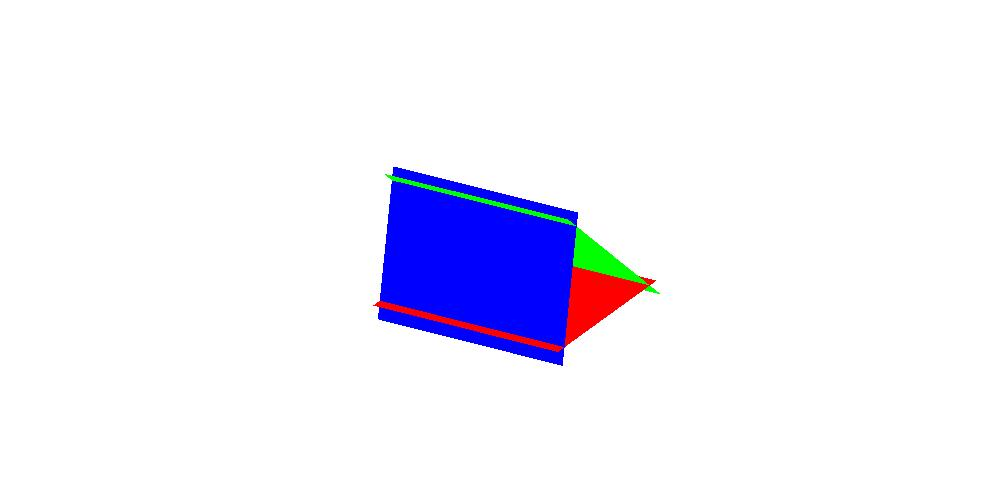
\includegraphics[scale=0.5,clip=true,
      trim=10cm 4.5cm 10cm 5.5cm]{images/toblerone}
 \]

\end{example}

\begin{example}\label{eg-lineq-ii}
 We will solve the equations
 \begin{align*}
  a + b + c + d &= 4 \\
  a + b - c - d &= 0 \\
  a - b + c - d &= 0 \\
  a - b - c + d &= 0.
 \end{align*}
 The corresponding augmented matrix can be row-reduced as follows:
 \[
  \left[\begin{array}{cccc|c}
    1 &  1 &  1 &  1 & 4 \\
    1 &  1 & -1 & -1 & 0 \\
    1 & -1 &  1 & -1 & 0 \\
    1 & -1 & -1 &  1 & 0
  \end{array}\right]
  \xra{1}
  \left[\begin{array}{cccc|c}
    1 &  1 &  1 &  1 &  4 \\
    0 &  0 & -2 & -2 & -4 \\
    1 & -1 &  1 & -1 & 0 \\
    0 &  0 & -2 &  2 & 0
  \end{array}\right]
  \xra{2}
  \left[\begin{array}{cccc|c}
    1 &  1 &  1 &  1 &  4 \\
    0 &  0 &  1 &  1 &  2 \\
    1 & -1 &  1 & -1 & 0 \\
    0 &  0 &  1 & -1 & 0
  \end{array}\right]
  \xra{3}
 \] \[
  \left[\begin{array}{cccc|c}
    1 &  1 &  0 &  0 & 2 \\
    0 &  0 &  1 &  1 & 2 \\
    1 & -1 &  0 &  0 & 0 \\
    0 &  0 &  1 & -1 & 0
  \end{array}\right]
  \xra{4}
  \left[\begin{array}{cccc|c}
    1 &  1 &  0 &  0 & 2 \\
    0 &  0 &  1 &  1 & 2 \\
    0 & -2 &  0 &  0 & -2 \\
    0 &  0 &  0 & -2 & -2
  \end{array}\right]
  \xra{5}
  \left[\begin{array}{cccc|c}
    1 &  1 &  0 &  0 & 2 \\
    0 &  0 &  1 &  1 & 2 \\
    0 &  1 &  0 &  0 & 1 \\
    0 &  0 &  0 &  1 & 1
  \end{array}\right]
  \xra{6}
 \] \[
  \left[\begin{array}{cccc|c}
    1 &  0 &  0 &  0 & 1 \\
    0 &  0 &  1 &  0 & 1 \\
    0 &  1 &  0 &  0 & 1 \\
    0 &  0 &  0 &  1 & 1
  \end{array}\right]
  \xra{7}
  \left[\begin{array}{cccc|c}
    1 &  0 &  0 &  0 & 1 \\
    0 &  1 &  0 &  0 & 1 \\
    0 &  0 &  1 &  0 & 1 \\
    0 &  0 &  0 &  1 & 1
  \end{array}\right]
 \]
 Here, rather than slavishly following Method~\ref{meth-RREF}, we have
 applied row operations in a more creative order to make the structure
 of the equations clearer.  The stages are as follows:
 \begin{itemize}
  \item[1] We subtract the first row from the second, and the third
   from the fourth.
  \item[2] We multiply the second and fourth rows by $-1/2$.
  \item[3] We subtract the second row from the first, and the fourth
   from the third.
  \item[4] We subtract the first row from the third, and the second
   from the fourth.
  \item[5] We multiply the third and fourth rows by $-1/2$.
  \item[6] We subtract the third row from the first, and the fourth
   from the second.
  \item[7] We exchange the second and third rows.
 \end{itemize}
 The final matrix corresponds to the equations $a=1$, $b=1$, $c=1$ and
 $d=1$, which give the unique solution to the original system of
 equations.
\end{example}

\begin{remark}
 Often we want to solve a \dfn{homogeneous} equation $Ax=0$, where
 the right hand side is zero.  This means that the relevant augmented
 matrix is $[A|0]$.  Row operations will not change the fact that the last
 column is zero, so the RREF of $[A|0]$ will just be $[A'|0]$, where
 $A'$ is the RREF of $A$.  In this context we can save writing by
 leaving out the extra column and just working with $A$.
\end{remark}
\begin{example}\label{eg-homogeneous}
 Consider the homogeneous system
 \begin{align*}
  a+b+c+d+e+f &= 0 \\
  2a+2b+2c+2d-e-f &= 0 \\
  3a+3b-c-d-e-f &= 0
 \end{align*}
 The corresponding unaugmented matrix can be row-reduced as follows:
 \[
  \bbm
    1 &  1 &  1 &  1 &  1 &  1 \\
    2 &  2 &  2 &  2 & -1 & -1 \\
    3 &  3 & -1 & -1 & -1 & -1
  \ebm \to \bbm
    1 &  1 &  0 &  0 &  0 &  0 \\
    0 &  0 &  1 &  1 &  0 &  0 \\
    0 &  0 &  0 &  0 &  1 &  1 
  \ebm
 \]
 (details are left to the reader).  The final matrix corresponds to
 the homogeneous system
 \[ a+b = 0 \hspace{5em} c+d=0 \hspace{5em} e+f=0. \]
 There are pivots in columns $1$, $3$ and $5$, meaning that $a$, $c$
 and $e$ are dependent variables, and $b$, $d$ and $f$ are
 independent.  After moving the independent variables to the right
 hand side, the solution becomes $a=-b$, $c=-d$ and $e=-f$.  If we
 prefer we can introduce new variables $\lm$, $\mu$ and $\nu$, and say
 that the general solution is
 \begin{align*}
  a &= -\lm & c &= -\mu & e &= -\nu \\
  b &=  \lm & d &=  \mu & f &=  \nu
 \end{align*}
 for arbitrary values of $\lm$, $\mu$ and $\nu$.
\end{example}

\section{Linear combinations}
\label{sec-lin-comb}

\begin{definition}\label{defn-lincomb}
 Let $v_1,\dotsc,v_k$ and $w$ be vectors in $\R^n$.  We say that $w$
 is a \dfn{linear combination} of $v_1,\dotsc,v_k$ if there exist
 scalars $\lm_1,\dots,\lm_k$ such that
 \[ w = \lm_1v_1 + \dotsb + \lm_kv_k. \]
\end{definition}

\begin{example}\label{eg-lincomb-i}
 Consider the following vectors in $\R^4$:
 \[ v_1 = \bbm 1 \\ -1 \\ 0 \\ 0 \ebm \hspace{3em}
    v_2 = \bbm 0 \\ 1 \\ -1 \\ 0 \ebm \hspace{3em}
    v_3 = \bbm 0 \\ 0 \\ 1 \\ -1 \ebm \hspace{3em}
    w   = \bbm 1 \\ 10 \\ 100 \\ -111 \ebm
 \]
 If we take $\lm_1=1$ and $\lm_2=11$ and $\lm_3=111$ we get
 \[ \lm_1 v_1 + \lm_2 v_2 + \lm_3 v_3 =
     \bbm 1 \\ -1 \\ 0 \\ 0 \ebm +
     \bbm 0 \\ 11 \\ -11 \\ 0 \ebm +
     \bbm 0 \\ 0 \\ 111 \\ -111 \ebm =
     \bbm 1 \\ 10 \\ 100 \\ -111 \ebm = w,
 \]
 which shows that $w$ is a linear combination of $v_1$, $v_2$ and
 $v_3$.
\end{example}

\begin{example}\label{eg-lincomb-ii}
 Consider the following vectors in $\R^4$:
 \[ v_1 = \bbm 0 \\ 1 \\  2 \\  3 \ebm \hspace{3em}
    v_2 = \bbm 0 \\ 1 \\  4 \\  9 \ebm \hspace{3em}
    v_3 = \bbm 0 \\ 1 \\  8 \\ 27 \ebm \hspace{3em}
    v_4 = \bbm 0 \\ 1 \\ 16 \\ 81 \ebm \hspace{3em}
    w = \bbm 1 \\ 1 \\ 1 \\ 1 \ebm.
 \]
 Any linear combination of $v_1,\dotsc,v_4$ has the form
 \[ \lm_1v_1 + \lm_2v_2 + \lm_3v_3 + \lm_4v_4 =
     \bbm 0 \\ \lm_1+\lm_2+\lm_3+\lm_4 \\
          2\lm_1+4\lm_2+8\lm_3+16\lm_4 \\
          3\lm_1+9\lm_2+27\lm_3+81\lm_4 \ebm.
 \]
 In particular, the first component of any such linear combination is
 zero.  (You should be able to see this without needing to write out
 the whole formula.)  As the first component of $w$ is not zero, we
 see that $w$ is \emph{not} a linear combination of $v_1,\dotsc,v_4$.
\end{example}

\begin{example}\label{eg-lincomb-iii}
 Consider the following vectors in $\R^3$:
 \[ v_1 = \bbm 1 \\ 1 \\ 1 \ebm \hspace{3em}
    v_2 = \bbm 1 \\ 2 \\ 1 \ebm \hspace{3em}
    v_3 = \bbm 1 \\ 3 \\ 1 \ebm \hspace{3em}
    v_4 = \bbm 1 \\ 4 \\ 1 \ebm \hspace{3em}
    v_5 = \bbm 1 \\ 5 \\ 1 \ebm \hspace{3em}
    w   = \bbm -1 \\ 0 \\ 1 \ebm.
 \]
 Any linear combination of $v_1,\dotsc,v_5$ has the form
 \[ \lm_1v_1 + \dotsb + \lm_5v_5 =
     \bbm \lm_1+\lm_2+\lm_3+\lm_4+\lm_5 \\
          \lm_1+2\lm_2+3\lm_3+4\lm_4+5\lm_5 \\
          \lm_1+\lm_2+\lm_3+\lm_4+\lm_5 \ebm.
 \]
 In particular, the first and last components of any such linear
 combination are the same.  Again, you should be able to see this
 without writing the full formula.  As the first and last components
 of $w$ are different, we see that $w$ is not a linear combination of
 $v_1,\dotsc,v_5$.
\end{example}
\begin{example}\label{eg-lincomb-iv}
 Let $v_1$, $v_2$ and $w$ be vectors in $\R^3$ (so we can think about
 them geometrically).  For simplicity, assume that all three vectors
 are nonzero, and that $v_1$ and $v_2$ do not point in the same
 direction, nor do they point in opposite directions.  This will mean
 that there is a unique plane $P$ that passes through $v_1$, $v_2$ and
 the origin.  It is not hard to see that $P$ is just the set of all
 possible linear combinations of $v_1$ and $v_2$.  Thus, our vector
 $w$ is a linear combination of $v_1$ and $v_2$ if and only if $w$
 lies in the plane $P$.
 \[ 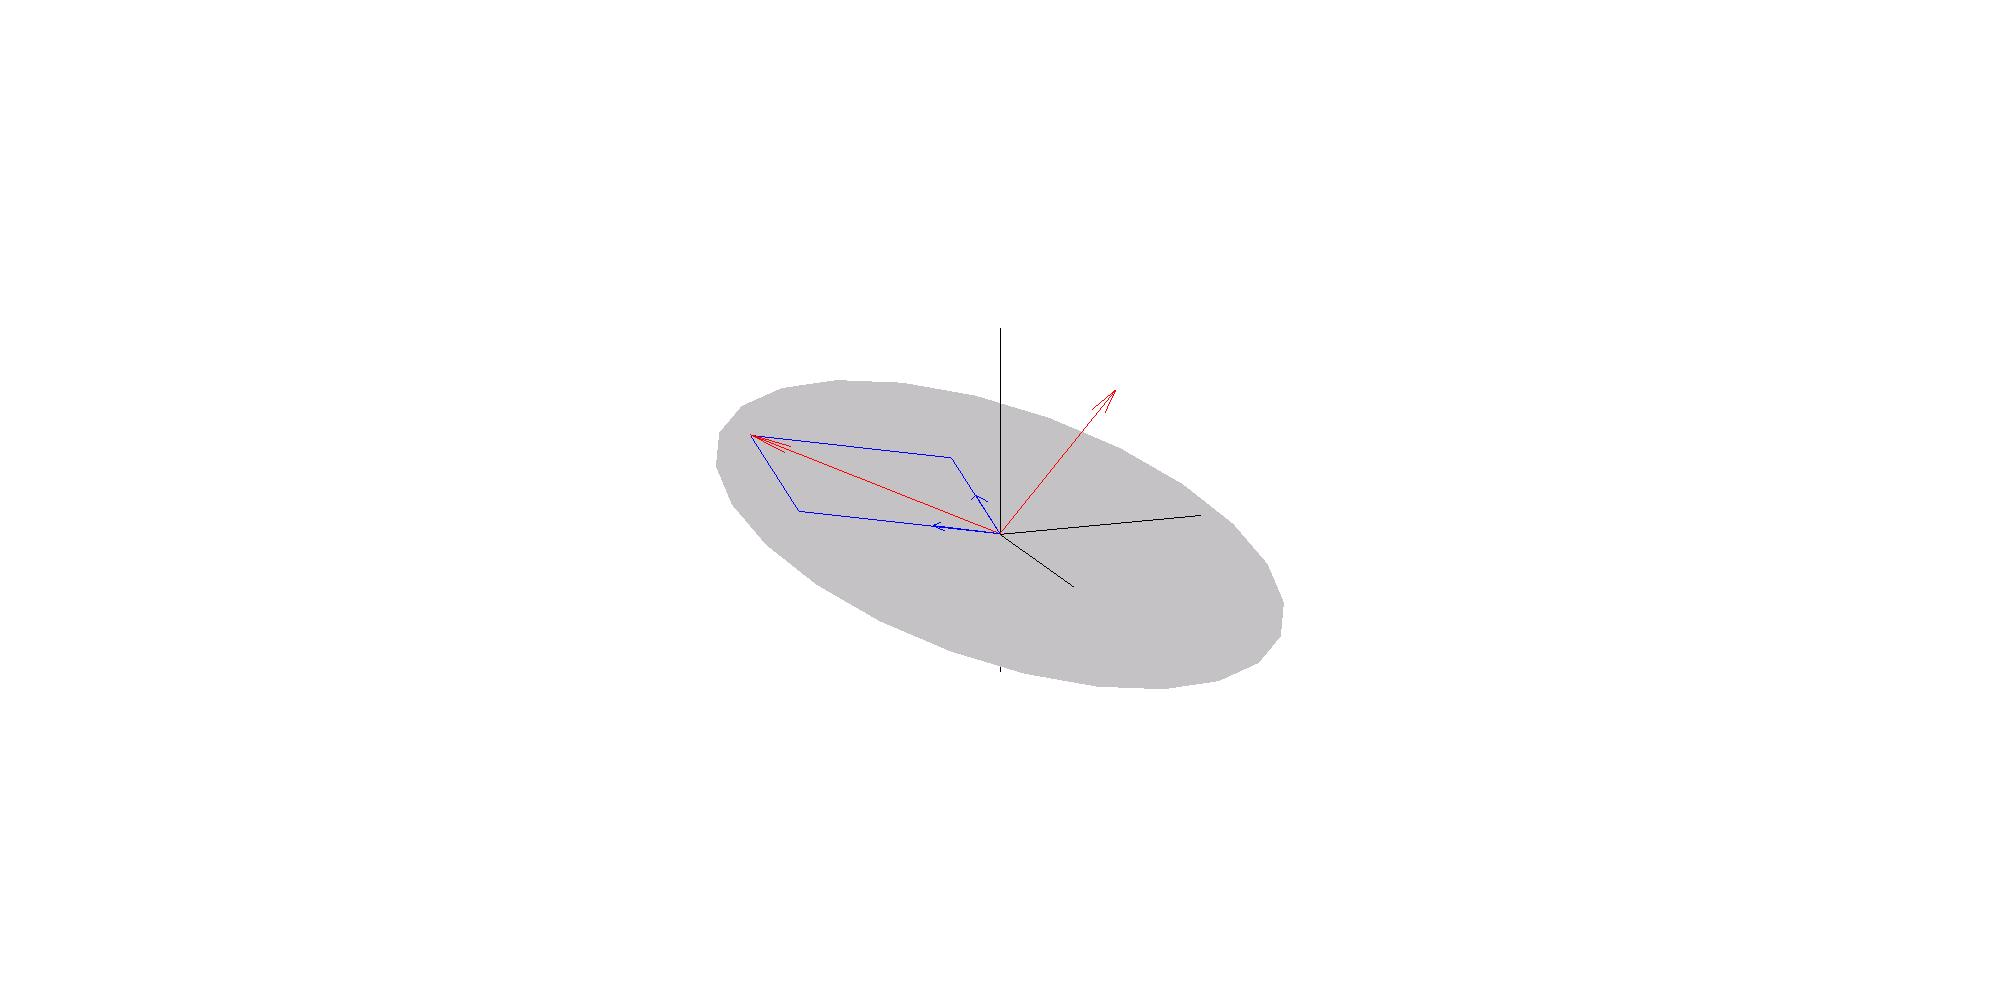
\includegraphics[scale=0.4,clip=true,
      trim=20cm 9cm 20cm 11cm]{images/plane_span}
 \]
\end{example}

We now want to explain a more systematic way to check whether a given
vector is a linear combination of some given list of vectors.
Note that for any $k$-vector
$\lm=\bbm\lm_1 & \dotsb & \lm_k\ebm^T$ we have
\[ A\lm =
    \left[\begin{array}{c|c|c}
     v_1 & \cdots & v_k
    \end{array}\right]
    \bbm \lm_1 \\ \vdots \\ \lm_k \ebm =
    \lm_1 v_1 + \dotsb + \lm_k v_k,
\]
which is the general form for a linear combination of
$v_1,\dotsc,v_k$.  This makes it clear that $w$ is a linear
combination of $v_1,\dotsc,v_k$ if and only if there is a vector $\lm$
which solves the matrix equation $A\lm=w$.  Using
Theorem~\ref{thm-row-ops} we see that the equation $A\lm=w$ has the
same solutions as the equation $A'\lm=w'$, which can be solved easily
by Method~\ref{meth-RREF-solve}.  We thus arrive at the following
method: 

\begin{method}\label{meth-find-lincomb}
 \index{linear combination}
 Suppose we have vectors $v_1,\dotsc,v_k\in\R^n$ and another vector
 $w\in\R^n$, and we want to express $w$ as a linear combination of the
 $v_i$ (or show that this is not possible).
 \begin{itemize}
  \item[(a)] We first let $A$ be the matrix whose columns are the
   vectors $v_i$:
   \[ A = \left[\begin{array}{c|c|c}
       v_1 & \cdots & v_k
      \end{array}\right] \in M_{n\tm k}(\R).
   \]
  \item[(b)] We then append $w$ as an additional column to get an
   augmented matrix
   \[ B  = \left[\begin{array}{c|c|c|c}
       v_1 & \cdots & v_k & w
      \end{array}\right]
       = \left[\begin{array}{c|c} A & w\end{array}\right].
   \]
   This corresponds to the matrix equation $A\lm=w$.
  \item[(c)] Row-reduce $B$ by Method~\ref{meth-RREF} to get a matrix
   $B'=[A'|w']$ in RREF.
  \item[(d)] If $B'$ has a pivot in the last column, then $w$ is not a
   linear combination of the vectors $v_1,\dotsc,v_k$.
  \item[(e)] If $B'$ has no pivot in the last column, then we can use
   Method~\ref{meth-RREF-solve} to find a vector
   $\lm=\bbm\lm_1 & \cdots & \lm_k\ebm^T$ satisfying $A'\lm=w'$.  We
   then have $A\lm=w$ and $\lm_1v_1+\dotsb+\lm_kv_k=w$, showing that
   $w$ is a linear combination of $v_1,\dotsc,v_k$.
 \end{itemize}
\end{method}

\begin{example}\label{eg-find-lincomb-i}
 Consider the vectors
 \[ v_1 = \bbm 11 \\ 11 \\ 1 \\ 1 \ebm \hspace{3em}
    v_2 = \bbm 1 \\ 11 \\ 11 \\ 1 \ebm \hspace{3em}
    v_3 = \bbm 1 \\ 1 \\ 11 \\ 11 \ebm \hspace{3em}
    w   = \bbm 121 \\ 221 \\ 1211 \\ 1111 \ebm.
 \]
 We ask whether $w$ can be expressed as a linear combination
 $w=\lm_1v_1+\lm_2v_2+\lm_3v_3$, and if so, what are the relevant
 values $\lm_1$, $\lm_2$ and $\lm_3$?  Following
 Method~\ref{meth-find-lincomb}, we write down the augmented
 matrix $[v_1|v_2|v_3|w]$ and row-reduce it:
 \[
  \left[\begin{array}{ccc|c}
   11 &  1 &  1 & 121 \\
   11 & 11 &  1 & 221 \\
    1 & 11 & 11 & 1211 \\
    1 &  1 & 11 & 1111
  \end{array}\right]
  \xra{1}
  \left[\begin{array}{ccc|c}
    1 &  1 & 11 & 1111 \\
   11 &  1 &  1 & 121 \\
   11 & 11 &  1 & 221 \\
    1 & 11 & 11 & 1211
  \end{array}\right]
  \xra{2}
  \left[\begin{array}{ccc|c}
    1 &   1 &   11 & 1111 \\
    0 & -10 & -120 & -12100 \\
    0 &   0 & -120 & -12000 \\
    0 &  10 &    0 & 100
  \end{array}\right]
  \xra{3}
 \] \[
  \left[\begin{array}{ccc|c}
    1 &   1 &   11 & 1111 \\
    0 &   1 &   12 & 1210 \\
    0 &   0 &    1 & 100 \\
    0 &   1 &    0 & 10
  \end{array}\right]
  \xra{4}
  \left[\begin{array}{ccc|c}
    1 &   1 &    0 & 11 \\
    0 &   1 &    0 & 10 \\
    0 &   0 &    1 & 100 \\
    0 &   1 &    0 & 10
  \end{array}\right]
  \xra{5}
  \left[\begin{array}{ccc|c}
    1 &   0 &    0 & 1 \\
    0 &   1 &    0 & 10 \\
    0 &   0 &    1 & 100 \\
    0 &   0 &    0 & 0
  \end{array}\right]
 \]
 (1: move the bottom row to the top; 2: subtract multiples of row 1
 from the other rows; 3: divide rows 2,3 and 4 by $-10$, $-120$ and
 $10$; 4: subtract multiples of row 3 from the other rows; 5: subtract
 multiples of row 2 from the other rows.)

 The final matrix corresponds to the system of equations
 \[ \lm_1 = 1 \hspace{3em}
    \lm_2 = 10 \hspace{3em}
    \lm_3 = 100 \hspace{3em}
     0 = 0
 \]
 so we conclude that
 \[ w = v_1 + 10 v_2 + 100 v_3. \]
 In particular, $w$ can be expressed as a linear combination of $v_1$,
 $v_2$ and $v_3$.  We can check the above equation directly:
 \[ v_1 + 10 v_2 + 100 v_3 =
      \bbm  11 \\  11 \\    1 \\    1 \ebm +
      \bbm  10 \\ 110 \\  110 \\   10 \ebm +
      \bbm 100 \\ 100 \\ 1100 \\ 1100 \ebm
    = \bbm 121 \\ 221 \\ 1211 \\ 1111 \ebm = w.
 \]
\end{example}

\begin{example}\label{eg-find-lincomb-ii}
 Consider the vectors
 \[ a_1 = \bbm 2 \\ -1 \\  0 \ebm \hspace{3em}
    a_2 = \bbm 3 \\  0 \\ -1 \ebm \hspace{3em}
    a_3 = \bbm 0 \\  3 \\ -2 \ebm \hspace{3em}
    b = \bbm 1 \\ 2 \\ 3 \ebm
 \]
 To test whether $b$ is a linear combination of $a_1$, $a_2$ and
 $a_3$, we write down the relevant augmented matrix and row-reduce it:
 \[
  \left[\begin{array}{ccc|c}
    2 &  3 &  0 & 1 \\
   -1 &  0 &  3 & 2 \\
    0 & -1 & -2 & 3
  \end{array}\right]
  \xra{1}
  \left[\begin{array}{ccc|c}
    1 &  0 & -3 & -2 \\
    0 &  1 &  2 & -3 \\
    2 &  3 &  0 &  1
  \end{array}\right]
  \xra{2}
  \left[\begin{array}{ccc|c}
    1 &  0 & -3 & -2 \\
    0 &  1 &  2 & -3 \\
    0 &  3 &  6 &  5
  \end{array}\right]
  \xra{3}
 \] \[
  \left[\begin{array}{ccc|c}
    1 &  0 & -3 & -2 \\
    0 &  1 &  2 & -3 \\
    0 &  0 &  0 & 14
  \end{array}\right]
  \xra{4}
  \left[\begin{array}{ccc|c}
    1 &  0 & -3 & -2 \\
    0 &  1 &  2 & -3 \\
    0 &  0 &  0 &  1
  \end{array}\right]
  \xra{5}
  \left[\begin{array}{ccc|c}
    1 &  0 & -3 &  0 \\
    0 &  1 &  2 &  0 \\
    0 &  0 &  0 &  1
  \end{array}\right]
 \]
 (Stage 1: move the top row to the bottom, and multiply the other two rows
 by $-1$; Stage 2: subtract $2$ times row 1 from row 3; Stage 3:
 subtract $3$ times row 2 from row 3; Stage 4: divide row 3 by $14$;
 Stage 5: subtract multiples of row 3 from rows 1 and 2.)

 The last matrix has a pivot in the rightmost column, corresponding to
 the equation $0=1$.  This means that the equation
 $\lm_1a_1+\lm_2a_2+\lm_3a_3=b$ cannot be solved for $\lm_1$, $\lm_2$
 and $\lm_3$, or in other words that $b$ is not a linear combination
 of $a_1$, $a_2$ and $a_3$.

 We can also see this in a more direct but less systematic way, as
 follows.  It is easy to check that $b.a_1=b.a_2=b.a_3=0$, which means
 that $b.(\lm_1a_1+\lm_2a_2+\lm_3a_3)=0$ for all possible choices of
 $\lm_1$, $\lm_2$ and $\lm_3$.  However, $b.b=14>0$, so $b$ cannot be
 equal to $\lm_1a_1+\lm_2a_2+\lm_3a_3$.
\end{example}

\section{Linear independence}

\begin{definition}\label{defn-dependent}
 Let $\CV=v_1,\dotsc,v_k$ be a list of vectors in $\R^n$.  A
 \dfn{linear relation} between the vectors $v_i$ is a relation of the
 form $\lm_1v_1+\dotsb+\lm_kv_k=0$, where $\lm_1,\dotsc,\lm_k$ are
 scalars.  In other words, it is a way of expressing $0$ as a linear
 combination of $\CV$.

 For any list we have the trivial linear relation
 $0v_1+0v_2+\dotsb+0v_k=0$.  There may or may not be any nontrivial
 linear relations.

 If the list $\CV$ has a nontrivial linear relation, we say that it is
 a \dfn{linearly dependent} list.  If the only linear relation on
 $\CV$ is the trivial one, we instead say that $\CV$ is \dfn{linearly
  independent}.  We will often omit the word ``linearly'' for the sake
 of brevity.
\end{definition}

\begin{example}\label{eg-dep-i}
 Consider the list $\CV$ given by
 \[ v_1 = \bbm 1 \\ 1 \\ 0 \\ 0 \ebm \hspace{3em}
    v_2 = \bbm 0 \\ 0 \\ 1 \\ 1 \ebm \hspace{3em}
    v_3 = \bbm 1 \\ 0 \\ 0 \\ 1 \ebm \hspace{3em}
    v_4 = \bbm 0 \\ 1 \\ 1 \\ 0 \ebm.
 \]
 There is a nontrivial linear relation $v_1+v_2-v_3-v_4=0$, so the
 list $\CV$ is dependent.
\end{example}
\begin{example}\label{eg-dep-ii}
 Consider the list $\CA$ given by
 \[ a_1 = \bbm  1 \\  2 \ebm \hspace{3em}
    a_2 = \bbm 12 \\  1 \ebm \hspace{3em}
    a_3 = \bbm -1 \\ -1 \ebm \hspace{3em}
    a_4 = \bbm  3 \\  1 \ebm.
 \]
 Just by writing it out, you can check that
 \[ 3a_1 + a_2 + 3a_3 -4a_4 = 0. \]
 \begin{center}
  \begin{tikzpicture}[scale=0.3]
   \fill( 0,0) circle(0.1);
   \fill( 3,6) circle(0.1);
   \fill(15,7) circle(0.1);
   \fill(12,4) circle(0.1);
   \draw[->, shorten >= 1pt] (0,0) -- (3,6);
   \draw[->, shorten >= 1pt] (3,6) -- (15,7);
   \draw[->, shorten >= 1pt] (15,7) -- (12,4);
   \draw[->, shorten >= 1pt] (12,4) -- (0,0);
   \draw ( 1.5,3.0) node[anchor=south east]{$\ss 3a_1$};
   \draw ( 9.0,6.5) node[anchor=south]{$\ss a_2$};
   \draw (13.5,5.5) node[anchor=north west]{$\ss 3a_3$};
   \draw ( 6.0,2.0) node[anchor=north]{$\ss -4a_4$};
  \end{tikzpicture}
 \end{center}
 This is a nontrivial linear relation on the list $\CA$, so $\CA$ is
 dependent.
\end{example}
\begin{example}\label{eg-indep-i}
 Consider the list $\CU$ given by
 \[ u_1 = \bbm 1 \\ 1 \\ 0 \\ 0 \ebm \hspace{3em}
    u_2 = \bbm 0 \\ 1 \\ 1 \\ 0 \ebm \hspace{3em}
    u_3 = \bbm 0 \\ 0 \\ 1 \\ 1 \ebm.
 \]
 We claim that this is independent.  To see this, consider a linear
 relation $\lm_1u_1+\lm_2u_2+\lm_3u_3=0$.  Writing this out, we get
 \[ \bbm \lm_1 \\ \lm_1+\lm_2 \\ \lm_2+\lm_3 \\ \lm_3 \ebm =
    \bbm 0 \\ 0 \\ 0 \\ 0 \ebm.
 \]
 By looking at the first and last rows we see that $\lm_1=\lm_3=0$.
 By looking at the second row we get $\lm_2=-\lm_1=0$ as well so our
 relation is the trivial relation.  As the only linear relation is the
 trivial one, we see that $\CU$ is independent.
\end{example}

\begin{lemma}\label{lem-multiples}
 Let $v$ and $w$ be vectors in $\R^n$, and suppose that $v\neq 0$ and
 that the list $(v,w)$ is linearly dependent.  Then there is a number
 $\al$ such that $w=\al v$.
\end{lemma}
\begin{proof}
 Because the list is dependent, there is a linear relation
 $\lm v+\mu w=0$ where $\lm$ and $\mu$ are not both zero.  There are
 apparently three possibilities: (a) $\lm\neq 0$ and $\mu\neq 0$; (b)
 $\lm=0$ and $\mu\neq 0$; (c) $\lm\neq 0$ and $\mu=0$.  However,
 case~(c) is not really possible.  Indeed, in case~(c) the equation
 $\lm v+\mu w=0$ would reduce to $\lm v=0$, and we could multiply by
 $\lm^{-1}$ to get $v=0$; but $v\neq 0$ by assumption.  In case~(a)
 or~(b) we can take $\al=-\lm/\mu$ and we have $w=\al v$.
\end{proof}

There is a systematic method using row-reduction for checking linear
(in)dependence, as we will explain shortly.  We first need a
preparatory observation.

\begin{definition}\label{defn-wide}
 Let $B$ be a $p\tm q$ matrix.  We say that $B$ is \dfn{wide} if
 $p<q$, or \dfn{square} if $p=q$ or \dfn{tall} if $p>q$.
 \[ \begin{array}{ccccc}
     \bbm 1 & 2 & 3 \\ 4 & 5 & 6 \ebm & &
     \bbm 1 & 2 & 1 \\ 2 & 3 & 2 \\ 1 & 2 & 1 \ebm & &
     \bbm 1 & 1 \\ 0 & 0 \\ 1 & 1 \ebm \\
     \text{ wide } & & \text{ square } & & \text{ tall }
    \end{array}
 \]
\end{definition}
\begin{lemma}\label{lem-pivots-everywhere}
 \index{pivot}
 Let $B$ be a $p\tm q$ matrix in RREF.
 \begin{itemize}
  \item[(a)] If $B$ is wide then it is impossible for every column to
   contain a pivot.
  \item[(b)] If $B$ is square then the only way for every column to
   contain a pivot is if $B=I_q$.
  \item[(c)] If $B$ is tall  then the only way for every column to
   contain a pivot is if $B$ consists of $I_q$ with $(p-q)$ rows of
   zeros added at the bottom (so
   $B=\left[\begin{array}{c} I_q \\ \hline 0_{(p-q)\tm q}
      \end{array}\right]$).
 \end{itemize}
\end{lemma}

For example, the only $5\tm 3$ RREF matrix with a pivot in every
column is this one:
\[ \left[\begin{array}{c}
      I_3 \\ \hline 0_{2\tm 3} 
   \end{array}\right] =
   \left[\begin{array}{ccc}
    1 & 0 & 0 \\
    0 & 1 & 0 \\
    0 & 0 & 1 \\ \hline
    0 & 0 & 0 \\
    0 & 0 & 0
   \end{array}\right]
\]

\begin{proof}
 There is at most one pivot in every row, making at most $p$ pivots
 altogether.  If $B$ is wide then we have $q$ columns with $q>p$, so
 there are not enough pivots to have one in every column.  This
 proves~(a).

 Now suppose instead that $B$ does have a pivot in every column, so
 there are $q$ pivots and we must have $p\geq q$.  As $B$ is in RREF
 we know that all entries above or below a pivot are zero.  As there
 is a pivot in every column it follows that the pivots are the only
 nonzero entries in $B$.  Every nonzero row contains precisely one
 pivot, so there must be $q$ nonzero rows.  The remaining $(p-q)$ rows
 are all zero, and they must occur at the bottom of $B$ (because $B$
 is in RREF).  Now the top $q\tm q$ block contains $q$ pivots which
 move to the right as we go down the matrix.  It is easy to see that
 the only possibility for the top block is $I_q$, which proves~(b)
 and~(c).
\end{proof}

\begin{method}\label{meth-check-dependence}
 \index{linearly dependent}\index{linearly independent}\index{pivot}
 Let $\CV=v_1,\dotsc,v_m$ be a list of vectors in $\R^n$.  We can
 check whether this list is dependent as follows.
 \begin{itemize}
  \item[(a)] Form the $n\tm m$ matrix
   \[ A = \left[\begin{array}{c|c|c}
              && \\
              v_1 & \dotsc & v_m \\
              &&
            \end{array}\right]
   \]
   whose columns are the vectors $v_i$.
  \item[(b)] Row reduce $A$ to get another $n\tm m$ matrix $B$ in
   RREF.
  \item[(c)] If every column of $B$ contains a pivot (so $B$ has the
   form discussed in Lemma~\ref{lem-pivots-everywhere}) then $\CV$ is
   independent.
  \item[(d)] If some column of $B$ has no pivot, then the list $\CV$
   is dependent.  Moreover, we can find the coefficients $\lm_i$ in a
   nontrivial linear relation by solving the vector equation $B\lm=0$
   (which is easy because $B$ is in RREF).
 \end{itemize}
\end{method}
\begin{remark}\label{rem-dependence-shortcut}
 \index{wide}\index{numerical criteria}
 If $m>n$ then $\CV$ is automatically dependent and we do not need to
 go through the method.  (For example, any list of $5$ vectors in
 $\R^3$ is automatically dependent, any list of $10$ vectors in $\R^9$
 is automatically dependent, and so on.)  Indeed, in this case the
 matrices $A$ and $B$ are wide, so it is impossible for $B$ to have a
 pivot in every column.  However, this line of argument only tells us
 that there \textbf{exists} a nontrivial relation
 $\lm_1v_1+\dotsb+\lm_mv_m=0$, it does not tell us the coefficients
 $\lm_i$.  If we want to find the $\lm_i$ then we do need to go
 through the whole method as explained above.
\end{remark}

We will give some examples of using the above method, and then explain
why the method is correct.

\begin{example}\label{eg-dep-i-matrix}
 In example~\ref{eg-dep-i} we considered the list
 \[ v_1 = \bbm 1 \\ 1 \\ 0 \\ 0 \ebm \hspace{3em}
    v_2 = \bbm 0 \\ 0 \\ 1 \\ 1 \ebm \hspace{3em}
    v_3 = \bbm 1 \\ 0 \\ 0 \\ 1 \ebm \hspace{3em}
    v_4 = \bbm 0 \\ 1 \\ 1 \\ 0 \ebm.
 \]
 We can write down the corresponding matrix and row-reduce it as
 follows:
 \[
  \bbm 1 & 0 & 1 & 0 \\
       1 & 0 & 0 & 1 \\
       0 & 1 & 0 & 1 \\
       0 & 1 & 1 & 0
  \ebm \xra{1}
  \bbm 1 & 0 & 1 & 0 \\
       0 & 0 &-1 & 1 \\
       0 & 1 & 0 & 1 \\
       0 & 0 & 1 &-1
  \ebm \xra{2}
  \bbm 1 & 0 & 1 & 0 \\
       0 & 1 & 0 & 1 \\
       0 & 0 & 1 &-1 \\
       0 & 0 &-1 & 1
  \ebm \xra{3}
  \bbm 1 & 0 & 0 & 1 \\
       0 & 1 & 0 & 1 \\
       0 & 0 & 1 &-1 \\
       0 & 0 & 0 & 0
  \ebm
 \]
 The end result has no pivot in the last column, so the original list is
 dependent.  To find a specific linear relation, we solve the equation
 \[   \bbm 1 & 0 & 0 & 1 \\
           0 & 1 & 0 & 1 \\
           0 & 0 & 1 &-1 \\
           0 & 0 & 0 & 0
      \ebm
      \bbm \lm_1 \\ \lm_2 \\ \lm_3 \\ \lm_4 \ebm =
      \bbm 0 \\ 0 \\ 0 \\ 0 \ebm
 \]
 to get $\lm_1=-\lm_4$, $\lm_2=-\lm_4$ and $\lm_3=\lm_4$ with $\lm_4$
 arbitrary.  Taking $\lm_4=1$ gives
 $(\lm_1,\lm_2,\lm_3,\lm_4)=(-1,-1,1,1)$, corresponding to the
 relation $-v_1-v_2+v_3+v_4=0$.
\end{example}
\begin{example}\label{eg-dep-ii-matrix}
 In Example~\ref{eg-dep-ii} we considered the list
 \[ a_1 = \bbm  1 \\  2 \ebm \hspace{3em}
    a_2 = \bbm 12 \\  1 \ebm \hspace{3em}
    a_3 = \bbm -1 \\ -1 \ebm \hspace{3em}
    a_4 = \bbm  3 \\  1 \ebm.
 \]
 Here we have $4$ vectors in $\R^2$, so they must be dependent by
 Remark~\ref{rem-dependence-shortcut}.  Thus, there exist nontrivial
 linear relations
 \[ \lm_1a_1 + \lm_2a_2 + \lm_3a_3 + \lm_4a_4 = 0. \]
 To actually find such a relation, we write down the corresponding
 matrix and row-reduce it as follows:
 \[
  \bbm
   1 & 12 & -1 & 3 \\
   2 & 1  & -1 & 1
  \ebm
  \xra{}
  \bbm
   1 &  12 & -1 & 3 \\
   0 & -23 &  1 & -5
  \ebm
  \xra{}
  \bbm
   1 &  12 & -1 & 3 \\
   0 &  1 & -1/23 & 5/23
  \ebm
  \xra{}
  \bbm
   1 &  0 & -11/23 & 9/23 \\
   0 &  1 & -1/23 & 5/23
  \ebm
 \]
 We now need to solve the matrix equation
 \[ \bbm
     1 &  0 & -11/23 & 9/23 \\
     0 &  1 & -1/23 & 5/23
    \ebm
    \bbm \lm_1 \\ \lm_2 \\ \lm_3 \\ \lm_4 \ebm =
    \bbm 0 \\ 0 \ebm
 \]
 As this is in RREF, we can just read off the solution:
 $\lm_1=\frac{11}{23}\lm_3-\frac{9}{23}\lm_4$ and
 $\lm_2=\frac{1}{23}\lm_3-\frac{5}{23}\lm_4$
 with $\lm_3$ and $\lm_4$ arbitrary.  If we choose $\lm_3=23$ and
 $\lm_4=0$ we get $(\lm_1,\lm_2,\lm_3,\lm_4)=(11,1,23,0)$ so we have a
 relation
 \[ 11 a_1 + a_2 + 23 a_3 + 0 a_4 = 0. \]
 (You should check directly that this is correct.)  Alternatively, we
 can choose $\lm_3=3$ and $\lm_4=-4$.  Using the equations
 $\lm_1=\frac{11}{23}\lm_3-\frac{9}{23}\lm_4$ and
 $\lm_2=\frac{1}{23}\lm_3-\frac{5}{23}\lm_4$ we get $\lm_1=3$ and
 $\lm_2=1$ giving a different relation
 \[ 3a_1 + a_2 + 3a_3 - 4a_4 = 0. \]
 This is the relation that we observed in Example~\ref{eg-dep-ii}.
\end{example}
\begin{example}\label{eg-indep-i-matrix}
 In Example~\ref{eg-indep-i} we considered the list $\CU$ given by
 \[ u_1 = \bbm 1 \\ 1 \\ 0 \\ 0 \ebm \hspace{3em}
    u_2 = \bbm 0 \\ 1 \\ 1 \\ 0 \ebm \hspace{3em}
    u_3 = \bbm 0 \\ 0 \\ 1 \\ 1 \ebm.
 \]
 We can write down the corresponding matrix and row-reduce it as
 follows:
 \[
  \bbm
   1 & 0 & 0 \\
   1 & 1 & 0 \\
   0 & 1 & 1 \\
   0 & 0 & 1
  \ebm
  \to
  \bbm
   1 & 0 & 0 \\
   0 & 1 & 0 \\
   0 & 1 & 1 \\
   0 & 0 & 1
  \ebm
  \to
  \bbm
   1 & 0 & 0 \\
   0 & 1 & 0 \\
   0 & 0 & 1 \\
   0 & 0 & 1
  \ebm
  \to
  \left[\begin{array}{ccc}
   1 & 0 & 0 \\
   0 & 1 & 0 \\
   0 & 0 & 1 \\ \hline
   0 & 0 & 0
  \end{array}\right]
 \]
 The final matrix has a pivot in every column, as in
 Lemma~\ref{lem-pivots-everywhere}.  It follows that the list $\CU$ is
 independent.
\end{example}

\begin{proof}[Proof of correctness of Method~\ref{meth-check-dependence}]
 Put
 \[ A = \left[\begin{array}{c|c|c}
              && \\
              v_1 & \cdots & v_m \\
              &&
        \end{array}\right]
 \]
 as in step~(a) of the method, and let $B$ be the RREF form of $A$.
 Note that for any vector
 $\lm=\bbm \lm_1 & \dotsc & \lm_m\ebm^T\in\R^m$, we have
 \[ A\lm =
     \left[\begin{array}{c|c|c}
              && \\
              v_1 & \cdots & v_m \\
              &&
     \end{array}\right]
     \bbm \lm_1 \\ \vdots \\ \lm_m \ebm =
     \lm_1v_1 + \dotsb + \lm_mv_m.
 \]
 Thus, linear relations on our list are just the same as solutions to
 the homogeneous equation $A\lm=0$.  By Theorem~\ref{thm-row-ops},
 these are the same as solutions to the equation $B\lm=0$, which can
 be found by Method~\ref{meth-RREF-solve}.  If there is a pivot in
 every column then none of the variables $\lm_i$ is independent, so
 the only solution is $\lm_1=\lm_2=\dotsb=\lm_m=0$.  Thus, the only
 linear relation on $\CV$ is the trivial one, which means that the
 list $\CV$ is linearly independent.

 Suppose instead that some column (the $k$'th one, say) does not
 contain a pivot.  Then in Method~\ref{meth-RREF-solve} the variable
 $\lm_k$ will be independent, so we can choose $\lm_k=1$.  This will
 give us a nonzero solution to $B\lm=0$, or equivalently $A\lm=0$,
 corresponding to a nontrivial linear relation on $\CV$.  This shows
 that $\CV$ is linearly dependent.
\end{proof}

\section{Spanning sets}
\label{sec-spanning}

\begin{definition}\label{defn-spanning-list}
 Suppose we have a list $\CV=v_1,\dotsc,v_m$ of vectors in $\R^n$.  We
 say that the list \emph{spans}\index{span} $\R^n$ if \textbf{every} vector in
 $\R^n$ can be expressed as a linear combination of $v_1,\dotsc,v_m$.
\end{definition}
\begin{example}\label{eg-not-span-i}
 Consider the list $\CV=v_1,v_2,v_3,v_4$, where
 \[ v_1 = \bbm 0 \\ 1 \\  2 \\  3 \ebm \hspace{3em}
    v_2 = \bbm 0 \\ 1 \\  4 \\  9 \ebm \hspace{3em}
    v_3 = \bbm 0 \\ 1 \\  8 \\ 27 \ebm \hspace{3em}
    v_4 = \bbm 0 \\ 1 \\ 16 \\ 81 \ebm
 \]
 In Example~\ref{eg-lincomb-ii} we saw that the vector
 $w=\bbm 1 & 1 & 1 & 1\ebm^T$ is not a linear combination of this
 list, so the list $\CV$ does not span $\R^4$.
\end{example}
\begin{example}\label{eg-not-span-ii}
 Consider the list $\CV=v_1,v_2,v_3,v_4,v_5$, where
 \[ v_1 = \bbm 1 \\ 1 \\ 1 \ebm \hspace{3em}
    v_2 = \bbm 1 \\ 2 \\ 1 \ebm \hspace{3em}
    v_3 = \bbm 1 \\ 3 \\ 1 \ebm \hspace{3em}
    v_4 = \bbm 1 \\ 4 \\ 1 \ebm \hspace{3em}
    v_5 = \bbm 1 \\ 5 \\ 1 \ebm.
 \]
 In Example~\ref{eg-lincomb-iii} we saw that the vector
 $w=\bbm -1 & 0 & 1 \ebm^T$ is not a linear combination of this
 list, so the list $\CV$ does not span $\R^3$.
\end{example}
\begin{example}\label{eg-not-span-iii}
 Similarly, Example~\ref{eg-find-lincomb-ii} shows that the list
 \[ \CA = \bbm 2 \\ -1 \\  0 \ebm, \qquad
          \bbm 3 \\  0 \\ -1 \ebm, \qquad
          \bbm 0 \\  3 \\ -2 \ebm
 \]
 does not span $\R^3$.
\end{example}

\begin{example}\label{eg-span-i}
 Consider the list $\CU=u_1,u_2,u_3$, where
 \[ u_1 = \bbm 1 \\ 1 \\ 0 \ebm \hspace{3em}
    u_2 = \bbm 1 \\ 0 \\ 1 \ebm \hspace{3em}
    u_3 = \bbm 0 \\ 1 \\ 1 \ebm.
 \]
 We will show that these span $\R^3$.  Indeed, for any vector
 $v=\bbm x & y & z\ebm^T\in\R^3$ we can put
 \[ \lm_1 = \frac{ x+y-z}{2} \hspace{4em}
    \lm_2 = \frac{ x-y+z}{2} \hspace{4em}
    \lm_3 = \frac{-x+y+z}{2}
 \]
 and we find that
 \begin{align*}
  \lm_1u_1+\lm_2u_2+\lm_3u_3
    &=
   \bbm (x+y-z)/2 \\ (x+y-z)/2 \\ 0 \ebm +
   \bbm (x-y+z)/2 \\ 0 \\ (x-y+z)/2 \ebm +
   \bbm 0 \\ (-x+y+z)/2 \\ (-x+y+z)/2 \ebm \\
    &=
   \bbm (x+y-z+x-y+z)/2 \\
        (x+y-z-x+y+z)/2 \\
        (x-y+z-x+y+z)/2 \ebm
    = \bbm x \\ y \\ z \ebm = v.
 \end{align*}
 This expresses $v$ as a linear combination of the list $\CU$, as
 required.
\end{example}

\begin{example}\label{eg-span-ii}
 Consider the list $\CA=a_1,a_2,a_3$ where
 \[ a_1 = \bbm 1 \\ 2 \ebm \hspace{3em}
    a_2 = \bbm 2 \\ 3 \ebm \hspace{3em}
    a_3 = \bbm 3 \\ 5 \ebm.
 \]
 Let $v=\bbm x \\ y\ebm$ be an arbitrary vector in $\R^2$.  Just by
 expanding out the right hand side, we see that
 \[ \bbm x \\ y \ebm =
     (2y-4x)\bbm 1 \\ 2 \ebm + (x-y)\bbm 2\\ 3\ebm + x\bbm 3\\5 \ebm,
 \]
 or in other words
 \[ v = (2y-4x)a_1 + (x-y)a_2 + x a_3. \]
 This expresses an arbitrary vector $v\in\R^2$ as a linear combination
 of $a_1$, $a_2$ and $a_3$, proving that the list $\CA$ spans $\R^2$.

 In this case there are actually many different ways in which we can
 express $v$ as a linear combination of $a_1$, $a_2$ and $a_3$.
 Another one is
 \[ v = (y-3x)a_1 + (2x-2y)a_2 + y a_3. \]
\end{example}

We now discuss a systematic method for spanning problems.

\begin{method}\label{meth-check-span}
 \index{span}\index{pivot}
 Let $\CV=v_1,\dotsc,v_m$ be a list of vectors in $\R^n$.  We can
 check whether this list spans $\R^n$ as follows.
 \begin{itemize}
  \item[(a)] Form the $m\tm n$ matrix
   \[ \renewcommand{\arraystretch}{1.3}
       C = \left[\begin{array}{ccc}
              & v_1^T & \\ \hline
              & \vdots & \\ \hline
              & v_m^T &
            \end{array}\right]
   \]
   whose rows are the row vectors $v_i^T$.
  \item[(b)] Row reduce $C$ to get another $m\tm n$ matrix $D$ in
   RREF.
  \item[(c)] If every column of $D$ contains a pivot (so $D$ has the
   form discussed in Lemma~\ref{lem-pivots-everywhere}) then $\CV$
   spans $\R^n$.
  \item[(d)] If some column of $D$ has no pivot, then the list $\CV$
   does not span $\R^n$.
 \end{itemize}
\end{method}
\begin{remark}\label{rem-dual-methods}
 This is almost exactly the same as
 Method~\ref{meth-check-dependence}, except that here we start by
 building a matrix whose rows are $v_i^T$, whereas in
 Method~\ref{meth-check-dependence} we start by building a matrix
 whose columns are $v_i$.  Equivalently, the matrix $C$ in this method
 is the transpose of the matrix $A$ in
 Method~\ref{meth-check-dependence}.  Note, however, that transposing
 does not interact well with row-reduction, so the matrix $D$ is
 \textbf{not} the transpose of $B$.
\end{remark}
\begin{remark}\label{rem-spanning-shortcut}
 \index{wide}\index{numerical criteria}
 If $m<n$ then the matrices $C$ and $D$ above will be wide, so $D$
 cannot have a pivot in every column, so the list $\CV$ cannot span
 $\R^n$.  For example, no list of $4$ vectors can span $\R^6$, and any
 list that spans $\R^8$ must contain at least $8$ vectors and so on.
\end{remark}

We will give some examples of using this method, then explain why it
works.
\begin{example}\label{eg-not-span-i-matrix}
 Consider the list
 \[ v_1 = \bbm 0 \\ 1 \\  2 \\  3 \ebm \hspace{3em}
    v_2 = \bbm 0 \\ 1 \\  4 \\  9 \ebm \hspace{3em}
    v_3 = \bbm 0 \\ 1 \\  8 \\ 27 \ebm \hspace{3em}
    v_4 = \bbm 0 \\ 1 \\ 16 \\ 81 \ebm
 \]
 as in Example~\ref{eg-not-span-i} (so $n=m=4$).  The relevant matrix
 $C$ is
 \[ C   = \bbm
           0 & 1 &  2 &  3 \\
           0 & 1 &  4 &  9 \\
           0 & 1 &  8 & 27 \\
           0 & 1 & 16 & 81
          \ebm
 \]
 The first column is zero, and will remain zero no matter what row
 operations we perform.  Thus $C$ cannot reduce to the identity
 matrix, so $\CV$ does not span (as we already saw by a different
 method).  In fact the row-reduction is
 \[ C \to \bbm 0 & 1 & 0 & 0 \\
               0 & 0 & 1 & 0 \\
               0 & 0 & 0 & 1 \\
               0 & 0 & 0 & 0 \ebm
 \]
 but it is not really necessary to go through the whole calculation.
\end{example}
\begin{example}\label{eg-not-span-ii-matrix}
 Consider the list
 \[ v_1 = \bbm 1 \\ 1 \\ 1 \ebm \hspace{3em}
    v_2 = \bbm 1 \\ 2 \\ 1 \ebm \hspace{3em}
    v_3 = \bbm 1 \\ 3 \\ 1 \ebm \hspace{3em}
    v_4 = \bbm 1 \\ 4 \\ 1 \ebm \hspace{3em}
    v_5 = \bbm 1 \\ 5 \\ 1 \ebm.
 \]
 as in Example~\ref{eg-not-span-ii} (so $n=3$ and $m=5$).  The
 relevant row-reduction is
 \[
  \bbm 1 & 1 & 1 \\ 1 & 2 & 1 \\ 1 & 3 & 1 \\ 1 & 4 & 1 \\ 1 & 5 & 1 \ebm
  \to
  \bbm 1 & 1 & 1 \\ 0 & 1 & 0 \\ 0 & 2 & 0 \\ 0 & 3 & 0 \\ 0 & 4 & 0 \ebm
  \to
  \left[\begin{array}{ccc}
   1 & 0 & 1 \\
   0 & 1 & 0 \\
   0 & 0 & 0 \\ \hline
   0 & 0 & 0 \\
   0 & 0 & 0 
  \end{array}\right]
 \]
 At the end of the process the last column does not contain a pivot
 (so the top $3\tm 3$ block is not the identity),
 so the original list does not span.  Again, we saw this earlier by a
 different method.
\end{example}
\begin{example}
 For the list
 \[ \CA = \bbm 2 \\ -1 \\  0 \ebm, \qquad
          \bbm 3 \\  0 \\ -1 \ebm, \qquad
          \bbm 0 \\  3 \\ -2 \ebm
 \]
 in Example~\ref{eg-not-span-iii}, the relevant row-reduction is
 \[ \bbm 2 & -1 & 0 \\ 3 & 0 & -1 \\ 0 & 3 & -2 \ebm \to
    \bbm 1 & -\half & 0 \\ 3 & 0 & -1 \\ 0 & 3 & -2 \ebm \to
    \bbm 1 & -\half & 0 \\ 0 & \tfrac{3}{2} & -1 \\ 0 & 3 & -2 \ebm \to
    \bbm 1 & -\half & 0 \\ 0 & 1 & -\tfrac{2}{3} \\ 0 & 0 & 0 \ebm \to
    \bbm 1 & 0 & -\tfrac{1}{3} \\ 0 & 1 & -\tfrac{2}{3} \\ 0 & 0 & 0 \ebm.
 \]
 In the last matrix the third column has no pivot, so the list does
 not span.
\end{example}
\begin{example}\label{eg-span-i-matrix}
 Consider the list $\CU=u_1,u_2,u_3$ from Example~\ref{eg-span-i}.
 \[ u_1 = \bbm 1 \\ 1 \\ 0 \ebm \hspace{3em}
    u_2 = \bbm 1 \\ 0 \\ 1 \ebm \hspace{3em}
    u_3 = \bbm 0 \\ 1 \\ 1 \ebm.
 \]
 The relevant row-reduction is
 \[ \bbm 1 & 1 & 0 \\ 1 &  0 &  1 \\ 0 & 1 & 1 \ebm \to
    \bbm 1 & 1 & 0 \\ 0 & -1 &  1 \\ 0 & 1 & 1 \ebm \to
    \bbm 1 & 1 & 0 \\ 0 &  1 & -1 \\ 0 & 0 & 2 \ebm \to
    \bbm 1 & 1 & 0 \\ 0 &  1 &  0 \\ 0 & 0 & 1 \ebm \to
    \bbm 1 & 0 & 0 \\ 0 &  1 &  0 \\ 0 & 0 & 1 \ebm
 \]
 The end result is the identity matrix, so the list $\CU$ spans
 $\R^3$.
\end{example}
\begin{example}
 Consider the list $\CA=\bbm 1\\2\ebm,\;\bbm 2\\3\ebm,\;\bbm 3\\5\ebm$
 from Example~\ref{eg-span-ii}.  The relevant row-reduction is
 \[ \bbm 1 & 2 \\ 2 & 3 \\ 3 & 5 \ebm \to
    \bbm 1 & 2 \\ 0 & -1 \\ 0 & -1 \ebm \to
    \bbm 1 & 2 \\ 0 &  1 \\ 0 & -1 \ebm \to
    \left[\begin{array}{cc}
     1 & 0 \\ 0 &  1 \\ \hline 0 & 0 
    \end{array}\right]
 \]
 In the last matrix, the top $2\tm 2$ block is the identity.  This
 means that the list $\CA$ spans $\R^2$.
\end{example}

We now explain why Method~\ref{meth-check-span} is valid.
\begin{lemma}\label{lem-span-invariant}
 \index{span}
 Let $C$ be an $m\tm n$ matrix, and let $C'$ be obtained from $C$ by a
 single elementary row operation.  Let $s$ be a row vector of length
 $n$.  Then $s$ can be expressed as a linear combination of the rows
 of $C$ if and only if it can be expressed as a linear combination of
 the rows of $C'$.
\end{lemma}
\begin{proof}
 Let the rows of $C$ be $r_1,\dotsc,r_m$.  Suppose that $s$ is a
 linear combination of these rows, say
 \[ s=\lm_1r_1+\lm_2r_2+\lm_3r_3+\dotsb+\lm_mr_m. \]
 \begin{itemize}
  \item[(a)] Suppose that $C'$ is obtained from $C$ by swapping the
   first two rows, so the rows of $C'$ are $r_2,r_1,r_3,\dotsc,r_m$.
   The sequence of numbers $\lm_2,\lm_1,\lm_3,\dotsc,\lm_m$ satisfies
   \[ s=\lm_2r_2+\lm_1r_1+\lm_3r_3+\dotsb+\lm_mr_m, \]
   which expresses $s$ as a linear combination of the rows of $C'$.  The
   argument is essentially the same if we exchange any other pair of
   rows.
  \item[(b)] Suppose instead that $C'$ is obtained from $C$ by
   multiplying the first row by a nonzero scalar $u$, so the rows of
   $C'$ are $ur_1,r_2,\dotsc,r_m$.  The sequence of numbers
   $u^{-1}\lm_1,\lm_2,\dotsc,\lm_m$ then satisfies
   \[ s = (u^{-1}\lm_1)(ur_1)+\lm_2r_2+\dotsb+\lm_mr_m, \]
   which expresses $s$ as a linear combination of the rows of $C'$.  The
   argument is essentially the same if we multiply any other row by a
   nonzero scalar.
  \item[(c)] Suppose instead that $C'$ is obtained from $C$ by adding
   $u$ times the second row to the first row, so the rows of $C'$ are
   $r_1+ur_2,r_2,r_3,\dotsc,r_m$.  The sequence of numbers
   $\lm_1,\lm_2-u\lm_1,\lm_3,\dotsc,\lm_n$ then satisfies
   \[ \lm_1(r_1+ur_2)+(\lm_2-u\lm_1)r_2+\lm_3r_3+\dotsb+\lm_mr_m =
       \lm_1r_1+\lm_2r_2+\dotsb+\lm_mr_m=s,
   \]
   which expresses $s$ as a linear combination of the rows of $C'$.  The
   argument is essentially the same if add a multiple of any row to
   any other row.
 \end{itemize}
 This proves half of the lemma: if $s$ is a linear combination of the
 rows of $C$, then it is also a linear combination of the rows of
 $C'$.  We also need to prove the converse: if $s$ is a linear
 combination of the rows of $C'$, then it is also a linear combination
 of the rows of $C$.  We will only treat case~(c), and leave the other
 two cases to the reader.  The rows of $C'$ are then
 $r_1+ur_2,r_2,r_3,\dotsc,r_m$.  As $s$ is a linear combination of
 these rows, we have $s=\mu_1(r_1+ur_2)+\mu_2r_2+\dotsb+\mu_mr_m$ for
 some numbers $\mu_1,\dotsc,\mu_m$.  Now the sequence of numbers
 $\mu_1,(\mu_2+u\mu_1),\mu_3,\dotsc,\mu_m$ satisfies
 \[ s = \mu_1r_1+(\mu_2+u\mu_1)r_2+\mu_3r_3+\dotsb+\mu_mr_m, \]
 which expresses $s$ as a linear combination of the rows of $C$.
\end{proof}

\begin{corollary}\label{cor-span-invariant}
 \index{span}
 Let $C$ be an $m\tm n$ matrix, and let $D$ be obtained from $C$ by a
 sequence of elementary row operation.  Let $s$ be a row vector of length
 $n$.  Then $s$ can be expressed as a linear combination of the rows
 of $C$ if and only if it can be expressed as a linear combination of
 the rows of $D$.
\end{corollary}
\begin{proof}
 Just apply the lemma to each step in the row-reduction sequence.
\end{proof}

\begin{lemma}\label{lem-check-span-RREF}
 \index{span}\index{pivot}
 Let $D$ be an $m\tm n$ matrix in RREF.
 \begin{itemize}
  \item[(a)] Suppose that every column of $D$ contains a pivot.  Then
   $m\geq n$, the top $n\tm n$ block of $D$ is the identity,  and
   everything below that block is zero.  In this case every row vector
   of length $n$ can be expressed as a linear combination of the rows
   of $D$.
  \item[(b)] Suppose instead that the $k$'th column of $D$ does not contain
   a pivot.  Then the standard basis vector $e_k$ \textbf{cannot} be
   expressed as a linear combination of the rows of $D$.
 \end{itemize}
\end{lemma}
\begin{proof}
 \begin{itemize}
  \item[(a)] Suppose that every column of $D$ contains a pivot.
   Lemma~\ref{lem-pivots-everywhere} tells us that $m\geq n$ and that
   $D=\left[\begin{array}{c} I_n \\ \hline 0_{(m-n)\tm n}\end{array}\right]$.
   Thus, the first $n$ rows are the standard basis vectors
   \begin{align*}
    r_1 &= e_1^T = \bbm 1 & 0 & 0 & \cdots & 0 \ebm \\
    r_2 &= e_2^T = \bbm 0 & 1 & 0 & \cdots & 0 \ebm \\
    r_3 &= e_3^T = \bbm 0 & 0 & 1 & \cdots & 0 \ebm \\
        & \cdots\cdots\cdots\cdots \\
    r_n &= e_n^T = \bbm 0 & 0 & 0 & \cdots & 1 \ebm
   \end{align*}
   and $r_i=0$ for $i>n$.  This means that any row vector
   $v=\bbm v_1 & v_2 & \cdots & v_n\ebm$ can be expressed as
   \begin{align*}
    v =& \bbm v_1 & 0 & 0 & \cdots & 0 \ebm + \\
       & \bbm 0 & v_2 & 0 & \cdots & 0 \ebm + \\
       & \bbm 0 & 0 & v_3 & \cdots & 0 \ebm + \\
       & \cdots\cdots\cdots\cdots\cdots\cdots\cdots + \\
       & \bbm 0 & 0 & 0 & \cdots & v_n \ebm  \\
      =& v_1r_1 + v_2r_2 + v_3r_3 + \dotsb + v_nr_n,
   \end{align*}
   which is a linear combination of the rows of $D$.
  \item[(b)] The argument here is most easily explained by an
   example.  Consider the matrix
   \[ D = \bbm 0 & 1 & 2 & 3 & 0 & 4 & 5 & 0 \\
               0 & 0 & 0 & 0 & 1 & 6 & 7 & 0 \\
               0 & 0 & 0 & 0 & 0 & 0 & 0 & 1 \ebm
   \]
   This is in RREF, with pivots in columns $2$, $5$ and $8$.  Let
   $r_i$ be the $i$'th row, and consider a linear combination
   \[ s = \lm_1r_1+\lm_2r_2+\lm_3r_3
        = \bbm 0 & \lm_1 & 2\lm_1 & 3\lm_1 &
               \lm_2 & 4\lm_1+6\lm_2 & 5\lm_1+7\lm_2 & \lm_3 \ebm.
   \]
   Note that the entries in the pivot columns $2$, $5$ and $8$ of $s$
   are just the coefficients $\lm_1$, $\lm_2$ and $\lm_3$.  This is
   not a special feature of this example: it simply reflects the fact
   that pivot columns contain nothing except the pivot.  Now choose a
   non-pivot column, say column number $6$, and consider the standard
   basis vector $e_6$.  Suppose we try to write $e_6$ as
   $\lm_1r_1+\lm_2r_2+\lm_3r_3$, or in other words to solve
   \[ \begin{array}{rccccccccl}
        [ & 0 & \RED{\mathbf{0}} & 0 & 0 &
          \RED{\mathbf{0}} & 1 & 0 & \RED{\mathbf{0}} & ] \\
       =[ & 0 & \RED{\mathbf{\lm_1}} & 2\lm_1 & 3\lm_1 &
           \RED{\mathbf{\lm_2}} & 4\lm_1+6\lm_2 &
            5\lm_1+7\lm_2 & \RED{\mathbf{\lm_3}} &].
      \end{array}
   \]
   By looking in column 2, we see that
   $\lm_1$ has to be zero.  By looking in column 5, we see that
   $\lm_2$ has to be zero.  By looking in column 8, we see that
   $\lm_3$ has to be zero.  This means that
   $\lm_1r_1+\lm_2r_2+\lm_3r_3=0$, so $\lm_1r_1+\lm_2r_2+\lm_3r_3$
   cannot be equal to $e_6$.

   This line of argument works more generally.  Suppose that $D$ is an
   RREF matrix and that the $k$'th column has no pivot.  We claim that
   $e_k$ is not a linear combination of the rows of $D$.  We can remove
   any rows of zeros from $D$ without affecting the question, so we
   may assume that every row is nonzero, so every row contains a
   pivot.  Suppose that $e_k=\lm_1r_1+\dotsb+\lm_mr_m$ say.  By
   looking in the column that contains the first pivot, we see that
   $\lm_1=0$.  By looking in the column that contains the second
   pivot, we see that $\lm_2=0$.  Continuing in this way, we see that
   all the coefficients $\lm_i$ are zero, so $\sum_i\lm_ir_i=0$, which
   contradicts the assumption that $e_k=\lm_1r_1+\dotsb+\lm_mr_m$.
 \end{itemize}
\end{proof}

\begin{proof}[Proof of correctness of Method~\ref{meth-check-span}]
 We form a matrix $C$ as in step~(b) of the method.  Recall that $\CV$
 spans $\R^n$ if and only if every column vector is a linear
 combination of the column vectors $v_i$.  It is clear that this
 happens if and only if every row vector is a linear combination of
 the row vectors $v_i^T$, which are the rows of $C$.  By
 Corollary~\ref{cor-span-invariant}, this happens if and only if every
 row vector is a linear combination of the rows of $D$.
 Lemma~\ref{lem-check-span-RREF} tells us that this happens if and
 only if $m\geq n$ and $D$ has a pivot in every column.
\end{proof}

We can now prove the following result, which is one of a number of
things that go by the name ``duality''.
\begin{proposition}\label{prop-duality}
 \index{duality}\index{span}\index{linearly independent}
 Let $P$ be an $m\tm n$ matrix.
 \begin{itemize}
  \item[(a)] The columns of $P$ are linearly independent in $\R^m$ if
   and only if the columns of $P^T$ span $\R^n$.
  \item[(b)] The columns of $P$ span $\R^m$ if and only if the columns
   of $P^T$ are linearly independent in $\R^n$.
 \end{itemize}
\end{proposition}
\begin{proof}
 Applying Method~\ref{meth-check-dependence} to the columns of $P$ is
 the same as applying Method~\ref{meth-check-span} to the columns of
 $P^T$.  Similarly, applying Method~\ref{meth-check-span} to the
 columns of $P$ is the same as applying
 Method~\ref{meth-check-dependence} to the columns of $P^T$.
\end{proof}

\begin{remark}\label{rem-duality}
 The way we have phrased the proposition reflects the fact that we
 have chosen to work with column vectors as far as possible.  However,
 one can define what it means for row vectors to span or be linearly
 independent, in just the same way as we did for column vectors.  We
 can then restate the proposition as follows:
 \begin{itemize}
  \item[(a)] The columns of $P$ are linearly independent if
   and only if the rows of $P$ span.
  \item[(b)] The columns of $P$ span if and only if the rows
   of $P$ are linearly independent.
 \end{itemize}
\end{remark}

\section{Bases}
\label{sec-bases}

\begin{definition}\label{defn-basis}
 A \dfn{basis} for $\R^n$ is a linearly independent list of vectors
 in $\R^n$ that also spans $\R^n$.
\end{definition}
\begin{remark}\label{rem-basis-length}
 Any basis for $\R^n$ must contain precisely $n$ vectors.  Indeed,
 Remark~\ref{rem-dependence-shortcut} tells us that a linearly
 independent list can contain at most $n$ vectors, and
 Remark~\ref{rem-spanning-shortcut} tells us that a spanning list must
 contain at least $n$ vectors.  As a basis has both these properties,
 it must contain precisely $n$ vectors.
\end{remark}

\begin{example}\label{eg-basis-i}
 Consider the list $\CU=(u_1,u_2,u_3)$, where
 \[ u_1 = \bbm 1 \\ 0 \\ 0 \ebm \hspace{3em}
    u_2 = \bbm 1 \\ 1 \\ 0 \ebm \hspace{3em}
    u_3 = \bbm 1 \\ 1 \\ 1 \ebm.
 \]
 For an arbitrary vector $v=\bbm a & b & c\ebm^T$ we have
 \[ (a-b)u_1 + (b-c)u_2 + cu_3 =
     \bbm a-b \\ 0 \\ 0 \ebm +
     \bbm b-c \\ b-c \\ 0 \ebm +
     \bbm c \\ c \\ c \ebm = \bbm a \\ b \\ c \ebm = v,
 \]
 which expresses $v$ as a linear combination of $u_1$, $u_2$ and
 $u_3$.  This shows that $\CU$ spans $\R^3$.  Now suppose we have a
 linear relation $\lm_1u_1+\lm_2u_2+\lm_3u_3=0$.  This means that
 \[ \bbm \lm_1+\lm_2+\lm_3 \\ \lm_2+\lm_3 \\ \lm_3 \ebm =
     \bbm 0 \\ 0 \\ 0 \ebm,
 \]
 from which we read off that $\lm_3=0$, then that $\lm_2=0$, then that
 $\lm_1=0$.  This means that the only linear relation on $\CU$ is the
 trivial one, so $\CU$ is linearly independent.  As it also spans, we
 conclude that $\CU$ is a basis.
\end{example}

\begin{proposition}\label{prop-basis}
 \index{basis}
 Suppose we have a list $\CV=(v_1,\dotsc,v_n)$ of $n$ vectors in
 $\R^n$, and we put
 \[ A = \left[\begin{array}{c|c|c}
              && \\
              v_1 & \dotsc & v_n \\
              &&
            \end{array}\right]
 \]
 (which is an $n\tm n$ square matrix).  Then $\CV$ is a basis if and
 only if the equation $A\lm=x$ has a \textbf{unique} solution for
 every $x\in\R^n$.
\end{proposition}
\begin{proof}
 \begin{itemize}
  \item[(a)]
   Suppose that $\CV$ is a basis.  In particular, this means that an
   arbitrary vector $x\in\R^n$ can be expressed as a linear combination
   \[ x = \lm_1v_1 + \dotsb + \lm_nv_n. \]
   Thus, if we form the vector $\lm=\bbm \lm_1 & \dotsb & \lm_n\ebm^T$,
   we have
   \[ A\lm = \left[\begin{array}{c|c|c}
              && \\ v_1 & \cdots & v_n \\ &&
             \end{array}\right]
             \bbm \lm_1 \\ \vdots \\ \lm_n \ebm
       = \lm_1v_1 + \dotsb + \lm_nv_n = x,
   \]
   so $\lm$ is a solution to the equation $A\lm=x$.  Suppose that $\mu$
   is another solution, so we also have
   \[ \mu_1v_1 + \dotsb + \mu_nv_n = x. \]
   By subtracting this from the earlier equation, we get
   \[ (\lm_1-\mu_1)v_1 + \dotsb + (\lm_n-\mu_n)v_n = 0. \]
   This is a linear relation on the list $\CV$.  However, $\CV$ is
   assumed to be a basis, so in particular it is linearly independent,
   so the only linear relation on $\CV$ is the trivial one.  This means
   that all the coefficients $\lm_i-\mu_i$ are zero, so the vector $\lm$
   is the same as the vector $\mu$.  In other words, $\lm$ is the
   \textbf{unique} solution to $A\lm=x$, as required.

  \item[(b)] We now need to prove the converse.  Suppose that for
   every $x\in\R^n$, the equation $A\lm=x$ has a unique solution.
   Equivalently, for every $x\in\R^n$, there is a unique sequence of
   coefficients $\lm_1,\dotsc,\lm_n$ such that
   $\lm_1v_1+\dotsc+\lm_nv_n=x$.  Firstly, we can temporarily ignore
   the uniqueness, and just note that every element $x\in\R^n$ can be
   expressed as a linear combination of $v_1,\dotsc,v_n$.  This means
   that the list $\CV$ spans $\R^n$.  Next, consider the case $x=0$.
   The equation $A\lm=0$ has $\lm=0$ as one solution.  By assumption,
   the equation $A\lm=0$ has a unique solution, so $\lm=0$ is the only
   solution.  Using the above equation for $A\lm$, we can restate this
   as follows: the only sequence $(\lm_1,\dotsc,\lm_n)$ for which
   $\lm_1v_1+\dotsb+\lm_nv_n=0$ is the sequence $(0,\dotsc,0)$.  In
   other words, the only linear relation on $\CV$ is the trivial one.
   This means that $\CV$ is linearly independent, and it also spans
   $\R^n$, so it is a basis.
 \end{itemize}
\end{proof}

This gives us a straightforward method to check whether a list is a
basis.
\begin{method}\label{meth-check-basis}
 \index{basis}
 Let $\CV=(v_1,\dotsc,v_m)$ be a list of vectors in $\R^n$.
 \begin{itemize}
  \item[(a)] If $m\neq n$ then $\CV$ is not a basis.
  \item[(b)] If $m=n$ then we form the matrix
   \[ A = \left[\begin{array}{c|c|c}
                && \\
                v_1 & \dotsc & v_m \\
                &&
              \end{array}\right]
   \]
   and row-reduce it to get a matrix $B$.
  \item[(c)] If $B=I_n$ then $\CV$ is a basis; otherwise, it is not.
 \end{itemize}
\end{method}

\begin{proof}[Proof of correctness of Method~\ref{meth-check-basis}]
 Step~(a) is justified by Remark~\ref{rem-basis-length}, so for the
 rest of the proof we can assume that $n=m$.

 Suppose that $A$ row-reduces to $I_n$.  Fix a vector $x\in\R^n$, and
 consider the equation $A\lm=x$.  This corresponds to the augmented
 matrix $[A|x]$.  If we perform the same row operations on $[A|x]$ as
 we did to convert $A$ to $I_n$, we will obtain a matrix of the form
 $[I_n|x']$.  Theorem~\ref{thm-row-ops} tells us that the solutions to
 $A\lm=x$ are the same as the solutions to $I_n\lm=x'$, so it is clear
 that $\lm=x'$ is the unique solution.  Thus the hypothesis of
 Proposition~\ref{prop-basis} is satisfied, and we can conclude that
 $\CV$ is a basis.

 Now suppose instead that row-reduction of $A$ leads to a matrix $B$
 in RREF that is not equal to $I_n$.  We know that $I_n$ is the only
 square RREF matrix with a pivot in every column, so $B$ cannot have a
 pivot in every column.  Method~\ref{meth-check-dependence} therefore
 tells us that the list $\CV$ is linearly dependent, so it cannot be a
 basis.
\end{proof}

\begin{example}\label{eg-not-basis}
 Consider the vectors
 \[
   v_1 = \bbm 1\\2\\3\\2\\1 \ebm \hspace{3em}
   v_2 = \bbm 3\\2\\1\\2\\3 \ebm \hspace{3em}
   v_3 = \bbm 1\\1\\1\\1\\1 \ebm \hspace{3em}
   v_4 = \bbm 1\\3\\5\\3\\1 \ebm \hspace{3em}
   v_5 = \bbm 5\\3\\1\\3\\5 \ebm
 \]
 To decide whether they form a basis, we construct the corresponding
 matrix $A$ and start row-reducing it:
 \[ \bbm 1&3&1&1&5 \\ 2&2&1&3&3 \\ 3&1&1&5&1 \\ 2&2&1&3&3 \\ 1&3&1&1&5 \ebm
    \to
    \bbm 1&3&1&1&5 \\ 0&-4&-1&1&-7 \\ 0&-8&-2&2&-14 \\ 0&-4&-1&1&-7 \\ 0&0&0&0&0 \ebm
    \to
    \bbm 1&3&1&1&5 \\ 0&-4&-1&1&-7 \\ 0&0&0&0&0 \\ 0&0&0&0&0 \\ 0&0&0&0&0 \ebm
 \]
 Already after the first step we have a row of zeros, and it is clear
 that we will still have a row of zeros after we complete the
 row-reduction, so $A$ does not reduce to the identity matrix, so the
 vectors $v_i$ do not form a basis.
\end{example}

\begin{example}\label{eg-basis-ii}
 Consider the vectors
 \[
  p_1 = \bbm  1 \\  1 \\ 11 \\  1 \ebm \hspace{3em}
  p_2 = \bbm  1 \\ 11 \\  1 \\ 11 \ebm \hspace{3em}
  p_3 = \bbm  1 \\  1 \\  1 \\ 11 \ebm \hspace{3em}
  p_4 = \bbm  1 \\ 11 \\ 11 \\ 11 \ebm
 \]
 To decide whether they form a basis, we construct the corresponding
 matrix $A$ and row reduce it:
 \[ \bbm  1 &  1 &  1 &  1 \\
          1 & 11 &  1 & 11 \\
         11 &  1 &  1 & 11 \\
          1 & 11 & 11 & 11 \ebm
    \to
    \bbm  1 &  1 &  1 &  1 \\
          0 & 10 &  0 & 10 \\
          0 &-10 &-10 &  0 \\
          0 & 10 & 10 & 10 \ebm
    \to
    \bbm  1 &  1 &  1 &  1 \\
          0 &  1 &  0 &  1 \\
          0 &  1 &  1 &  0 \\
          0 &  1 &  1 &  1 \ebm
    \to
 \] \[
    \bbm  1 &  1 &  1 &  1 \\
          0 &  1 &  0 &  1 \\
          0 &  1 &  1 &  0 \\
          0 &  0 &  0 &  1 \ebm
    \to
    \bbm  1 &  1 &  1 &  1 \\
          0 &  1 &  0 &  1 \\
          0 &  0 &  1 & -1 \\
          0 &  0 &  0 &  1 \ebm
    \to
    \bbm  1 &  0 &  1 &  0 \\
          0 &  1 &  0 &  1 \\
          0 &  0 &  1 & -1 \\
          0 &  0 &  0 &  1 \ebm
 \]
 After a few more steps, we obtain the identity matrix.  It follows
 that the list $p_1,p_2,p_3,p_4$ is a basis.
\end{example}

Now suppose that the list $\CV=v_1,\dotsc,v_n$ is a basis for $\R^n$,
and that $w$ is another vector in $\R^n$.  By the very definition of a
basis, it must be possible to express $w$ (in a unique way) as a
linear combination $w=\lm_1v_1+\dotsb+\lm_nv_n$.  If we want to find
the coefficients $\lm_i$, we can use Method~\ref{meth-find-lincomb}.
That method can be streamlined slightly in this context, as follows.

\begin{method}\label{meth-find-lincomb-basis}
 Let $\CV=v_1,\dotsc,v_n$ be a basis for $\R^n$, and let $w$ be
 another vector in $\R^n$.
 \begin{itemize}
  \item[(a)] Let $B$ be the matrix
   \[ B = \left[\begin{array}{c|c|c|c}
       v_1 & \cdots & v_n & w
      \end{array}\right] \in M_{n\tm (n+1)}(\R).
   \]
  \item[(b)] Let $B'$ be the RREF form of $B$.  Then $B'$ will have
   the form $[I_n|\lm]$ for some column vector
   \[ \lm = \bbm \lm_1 \\ \vdots \\ \lm_n \ebm. \]
  \item[(c)] Now $w=\lm_1v_1+\dotsb+\lm_nv_n$.
 \end{itemize}
\end{method}
It is clear from our discussion  of Method~\ref{meth-find-lincomb} and
Method~\ref{meth-check-basis} that this is valid.

\begin{example}
 We will express the vector $q=\bbm 0.9 \\ 0.9 \\ 0 \\ 10.9 \ebm$ in terms
 of the basis $p_1,p_2,p_3,p_4$ introduced in Example~\ref{eg-basis-ii}.
 We form the relevant augmented matrix, and apply the same
 row-reduction steps as in Example~\ref{eg-basis-ii}, except that we now
 have an extra column.
 \[ \left[\begin{array}{cccc|c}
          1 &  1 &  1 &  1 &  0.9\\
          1 & 11 &  1 & 11 &  0.9\\
         11 &  1 &  1 & 11 &  0  \\
          1 & 11 & 11 & 11 & 10.9
    \end{array}\right]
    \to
    \left[\begin{array}{cccc|c}
          1 &  1 &  1 &  1 & 0.9 \\
          0 & 10 &  0 & 10 & 0   \\
          0 &-10 &-10 &  0 & -9.9\\
          0 & 10 & 10 & 10 & 10
    \end{array}\right]
    \to
    \left[\begin{array}{cccc|c}
          1 &  1 &  1 &  1 & 0.9 \\
          0 &  1 &  0 &  1 & 0   \\
          0 &  1 &  1 &  0 & 0.99\\
          0 &  1 &  1 &  1 & 1
    \end{array}\right]
    \to
 \] \[
    \left[\begin{array}{cccc|c}
          1 &  1 &  1 &  1 & 0.9 \\
          0 &  1 &  0 &  1 & 0   \\
          0 &  1 &  1 &  0 & 0.99 \\
          0 &  0 &  0 &  1 & 0.01
    \end{array}\right]
    \to
    \left[\begin{array}{cccc|c}
          1 &  1 &  1 &  1 & 0.9 \\
          0 &  1 &  0 &  1 & 0   \\
          0 &  0 &  1 & -1 & 0.99\\
          0 &  0 &  0 &  1 & 0.01
    \end{array}\right]
    \to
    \left[\begin{array}{cccc|c}
          1 &  0 &  1 &  0 & 0.9 \\
          0 &  1 &  0 &  1 & 0   \\
          0 &  0 &  1 & -1 & 0.99\\
          0 &  0 &  0 &  1 & 0.01
    \end{array}\right] \to
 \] \[
    \left[\begin{array}{cccc|c}
          1 &  0 &  1 &  0 & 0.9 \\
          0 &  1 &  0 &  0 &-0.01 \\
          0 &  0 &  1 &  0 & 1 \\
          0 &  0 &  0 &  1 & 0.01
    \end{array}\right]
    \to
    \left[\begin{array}{cccc|c}
          1 &  0 &  0 &  0 &-0.1 \\
          0 &  1 &  0 &  0 &-0.01 \\
          0 &  0 &  1 &  0 & 1 \\
          0 &  0 &  0 &  1 & 0.01
    \end{array}\right]
 \]
 The final result is $[I_4|\lm]$, where
 $\lm=\bbm -0.1&-0.01&1&0.01\ebm^T$.  This means that $q$ can be
 expressed in terms of the vectors $p_i$ as follows:
 \[ q = -0.1 p_1 - 0.01 p_2 + p_3 + 0.01 p_4. \]
\end{example}

\begin{example}
 One can check that the vectors $u_1$, $u_2$, $u_3$ and $u_4$ below
 form a basis for $\R^4$.
 \[ \renewcommand{\arraystretch}{1.2}
  u_1 = \bbm 1            \\ \tfrac{1}{2} \\ \tfrac{1}{3} \\ \tfrac{1}{4} \ebm
  \hspace{3em}
  u_2 = \bbm \tfrac{1}{2} \\ \tfrac{1}{3} \\ \tfrac{1}{4} \\ \tfrac{1}{5} \ebm
  \hspace{3em}
  u_3 = \bbm \tfrac{1}{3} \\ \tfrac{1}{4} \\ \tfrac{1}{5} \\ \tfrac{1}{6} \ebm
  \hspace{3em}
  u_4 = \bbm \tfrac{1}{4} \\ \tfrac{1}{5} \\ \tfrac{1}{6} \\ \tfrac{1}{7} \ebm
  \hspace{3em}
  v = \bbm 1 \\ 1 \\ 1 \\ 1 \ebm
 \]
 We would like to express $v$ in terms of this basis.  The matrix
 formed by the vectors $u_i$ is called the \dfn{Hilbert matrix}; it
 is notoriously hard to row-reduce.  We will therefore use Maple:
 \begin{verbatim}
with(LinearAlgebra):
RREF := ReducedRowEchelonForm;
u[1] := <1,1/2,1/3,1/4>;
u[2] := <1/2,1/3,1/4,1/5>;
u[3] := <1/3,1/4,1/5,1/6>;
u[4] := <1/4,1/5,1/6,1/7>;
v    := <1,1,1,1>;
B    := <u[1]|u[2]|u[3]|u[4]|v>;
RREF(B);
 \end{verbatim}
 Maple tells us that
 \[ \left[\begin{array}{cccc|c}
          1 &  1/2 &  1/3 &  1/4 &  1 \\
        1/2 &  1/3 &  1/4 &  1/5 &  1 \\
        1/3 &  1/4 &  1/5 &  1/6 &  1 \\
        1/4 &  1/5 &  1/6 &  1/7 &  1 \\
    \end{array}\right]
    \to
    \left[\begin{array}{cccc|c}
          1 &  0 &  0 &  0 & -4  \\
          0 &  1 &  0 &  0 & 60  \\
          0 &  0 &  1 &  0 & -180\\
          0 &  0 &  0 &  1 & 140
    \end{array}\right].
 \]
 We conclude that
 \[ v = -4 u_1 + 60 u_2 -180 u_3 + 140 u_4. \]
 The equivalent in Python with SymPy is to enter 
\begin{verbatim}
B = Matrix([
 [1,1/2,1/3,1/4],
 [1/2,1/3,1/4,1/5],
 [1/3,1/4,1/5,1/6],
 [1/4,1/5,1/6,1/7],
 [1,1,1,1]
]).T
B.rref()[0]
\end{verbatim}
\end{example}

\begin{proposition}\label{prop-duality-bases}
 \index{duality}\index{basis}
 Let $A$ be an $n\tm n$ matrix.  Then the columns of $A$ form a basis
 for $\R^n$ if and only if the columns of $A^T$ form a basis for
 $\R^n$.
\end{proposition}
\begin{proof}
 Suppose that the columns of $A$ form a basis.  This means in
 particular that the columns of $A$ are linearly independent, so the
 columns of $A^T$ span $\R^n$ by part~(a) of
 Proposition~\ref{prop-duality}.  Also, the columns of $A$ must span
 $\R^n$ (by the other half of the definition of a basis) so the
 columns of $A^T$ are linearly independent by part~(b) of
 Proposition~\ref{prop-duality}.  As the columns of $A^T$ are linearly
 independent and span $\R^n$, they form a basis.

 The converse is proved in the same way.
\end{proof}

\begin{proposition}\label{prop-basis-numerical}
 \index{basis}\index{numerical criteria}
 Let $\CV$ be a list of $n$ vectors in $\R^n$ (so the number of
 vectors is the same as the number of entries in each vector).
 \begin{itemize}
  \item[(a)] If the list is linearly independent then it also spans,
   and so is a basis.
  \item[(b)] If the list spans then it is also linearly independent,
   and so is a basis.
 \end{itemize}
 (However, these rules are \textbf{not valid} for lists of length
 different from $n$.)
\end{proposition}
\begin{proof}
 Let $A$ be the matrix whose columns are the vectors in $\CV$.
 \begin{itemize}
 \item[(a)] Suppose that $\CV$ is linearly independent.  Let $B$ be
  the matrix obtained by row-reducing $A$.
  Method~\ref{meth-check-dependence} tells us that $B$ has a pivot in
  every column.  As $B$ is also square, we must have $B=I_n$.
  Method~\ref{meth-check-basis} therefore tells us that $\CV$ is a
  basis.
 \item[(b)] Suppose instead that $\CV$ (which is the list of columns
  of $A$) spans $\R^n$.  By Proposition~\ref{prop-duality}, we
  conclude that the columns of $A^T$ are linearly independent.  Now
  $A^T$ has $n$ columns, so we can apply part~(a) to deduce that the
  columns of $A^T$ form a basis.  By
  Proposition~\ref{prop-duality-bases}, the columns of $A$ must form a
  basis as well.
 \end{itemize}
\end{proof}

\section{Elementary matrices and invertibility}
\label{sec-elem}

\begin{definition}\label{defn-elementary}
 Fix an integer $n \geq 0$.  We define $n\tm n$ matrices as follows.
 \begin{itemize}
  \item[(a)] Suppose that $1\leq p\leq n$ and that $\lm$ is a nonzero
   real number.  We then let $D_p(\lm)$ be the matrix that is the same
   as $I_n$ except that $(D_p(\lm))_{pp}=\lm$.
  \item[(b)] Suppose that $1\leq p,q\leq n$ with $p\neq q$, and that
   $\mu$ is an arbitrary real number.  We then let $E_{pq}(\mu)$ be
   the matrix that is the same as $I_n$ except that
   $(E_{pq}(\mu))_{pq}=\mu$.
  \item[(c)] Suppose again that $1\leq p,q\leq n$ with $p\neq q$.  We
   let $F_{pq}$ be the matrix that is the same as $I_n$ except that
   $(F_{pq})_{pp}=(F_{pq})_{qq}=0$ and $(F_{pq})_{pq}=(F_{pq})_{qp}=1$.
 \end{itemize}
 An \dfn{elementary matrix} is a matrix of one of these types.
\end{definition}

\begin{example}\label{eg-elementary}
 In the case $n=4$, we have
 \[
   D_2(\lm) =
    \bbm
     1 & 0 & 0 & 0 \\
     0 & \lm & 0 & 0 \\
     0 & 0 & 1 & 0 \\
     0 & 0 & 0 & 1
    \ebm
   \hspace{3em}
   E_{24}(\mu) =
    \bbm
     1 & 0 & 0 & 0 \\
     0 & 1 & 0 & \mu \\
     0 & 0 & 1 & 0 \\
     0 & 0 & 0 & 1
    \ebm
   \hspace{3em}
   F_{24} =
    \bbm
     1 & 0 & 0 & 0 \\
     0 & 0 & 0 & 1 \\
     0 & 0 & 1 & 0 \\
     0 & 1 & 0 & 0
    \ebm
 \]
\end{example}

Elementary matrices correspond precisely to row operations, as
explained in the next result.

\begin{proposition}\label{prop-ro-elem}
 \index{elementary matrix}\index{row operation}
 Let $A$ be an $n\tm m$ matrix, and let $A'$ be obtained from $A$ by a
 single row operation.  Then $A'=UA$ for some elementary matrix
 $U \in M_n(\R)$.
 In more detail:
 \begin{itemize}
  \item[(a)] Let $A'$ be obtained from $A$ by multiplying the $p$'th
   row by $\lm$.  Then $A'=D_p(\lm)A$.
  \item[(b)] Let $A'$ be obtained from $A$ by adding $\mu$ times the
   $q$'th row to the $p$'th row.  Then $A'=E_{pq}(\mu)A$.
  \item[(c)] Let $A'$ be obtained from $A$ by exchanging the $p$'th
   row and the $q$'th row.  Then $A'=F_{pq}A$.
 \end{itemize}
\end{proposition}

\begin{proof}
We will not give a formal proof, as examples are more illuminating:
if we take
\[ A = \bbm
        a_{11} & a_{12} & a_{13} & a_{14} \\
        a_{21} & a_{22} & a_{23} & a_{24} \\
        a_{31} & a_{32} & a_{33} & a_{34} \\
        a_{41} & a_{42} & a_{43} & a_{44}
       \ebm
\]
then
\begin{align*}
 D_2(\lm)A &=
    \bbm
     1 & 0 & 0 & 0 \\
     0 & \lm & 0 & 0 \\
     0 & 0 & 1 & 0 \\
     0 & 0 & 0 & 1
    \ebm
    \bbm
     a_{11} & a_{12} & a_{13} & a_{14} \\
     a_{21} & a_{22} & a_{23} & a_{24} \\
     a_{31} & a_{32} & a_{33} & a_{34} \\
     a_{41} & a_{42} & a_{43} & a_{44}
    \ebm
    =
    \bbm
     a_{11} & a_{12} & a_{13} & a_{14} \\
     \lm a_{21} & \lm a_{22} & \lm a_{23} & \lm a_{24} \\
     a_{31} & a_{32} & a_{33} & a_{34} \\
     a_{41} & a_{42} & a_{43} & a_{44}
    \ebm \\
 E_{24}(\mu)A &=
    \bbm
     1 & 0 & 0 & 0 \\
     0 & 1 & 0 & \mu \\
     0 & 0 & 1 & 0 \\
     0 & 0 & 0 & 1
    \ebm
    \bbm
     a_{11} & a_{12} & a_{13} & a_{14} \\
     a_{21} & a_{22} & a_{23} & a_{24} \\
     a_{31} & a_{32} & a_{33} & a_{34} \\
     a_{41} & a_{42} & a_{43} & a_{44}
    \ebm
    =
    \bbm
     a_{11} & a_{12} & a_{13} & a_{14} \\
     a_{21}+\mu a_{41} & a_{22}+\mu a_{42} & a_{23}+\mu a_{43} & a_{24}+\mu a_{44} \\
     a_{31} & a_{32} & a_{33} & a_{34} \\
     a_{41} & a_{42} & a_{43} & a_{44}
    \ebm \\
 F_{24}A &=
    \bbm
     1 & 0 & 0 & 0 \\
     0 & 0 & 0 & 1 \\
     0 & 0 & 1 & 0 \\
     0 & 1 & 0 & 0
    \ebm
    \bbm
     a_{11} & a_{12} & a_{13} & a_{14} \\
     a_{21} & a_{22} & a_{23} & a_{24} \\
     a_{31} & a_{32} & a_{33} & a_{34} \\
     a_{41} & a_{42} & a_{43} & a_{44}
    \ebm
    =
    \bbm
     a_{11} & a_{12} & a_{13} & a_{14} \\
     a_{41} & a_{42} & a_{43} & a_{44} \\
     a_{31} & a_{32} & a_{33} & a_{34} \\
     a_{21} & a_{22} & a_{23} & a_{24}
    \ebm
    \qedhere
\end{align*}
\end{proof}

\begin{corollary}\label{cor-ro-elem}
 \index{elementary matrix}\index{row operation}
 Let $A$ and $B$ be $n\tm m$ matrices, and suppose that $A$ can be
 converted to $B$ by a sequence of row operations.  Then $B=UA$ for
 some $n\tm n$ matrix $U$ that can be expressed as a product of
 elementary matrices.
\end{corollary}
\begin{proof}
 The assumption is that there is a sequence of $n\tm m$ matrices
 $A_0,A_1,\dotsc,A_r$ starting with $A_0=A$ and ending with $A_r=B$
 such that $A_i$ is obtained from $A_{i-1}$ by a single row
 operation.  By the Proposition, this means that there is an
 elementary matrix $U_i$ such that $A_i=U_iA_{i-1}$.  This gives
 \begin{align*}
  A_1 &= U_1A_0 = U_1A \\
  A_2 &= U_2A_1 = U_2U_1A \\
  A_3 &= U_3A_2 = U_3U_2U_1A
 \end{align*}
 and so on.  Eventually we get $B=A_r=U_rU_{r-1}\dotsb U_1A$.  We can
 thus take $U=U_rU_{r-1}\dotsb U_1$ and we have $B=UA$ as required.
\end{proof}

\begin{theorem}\label{thm-inverse}
 \index{invertible}\index{basis}\index{linearly independent}\index{span}
 \index{transpose}\index{duality}
 Let $A$ be an $n\tm n$ matrix.  Then the following statements are
 equivalent: if any one of them is true then they are all true, and if
 any one of them is false then they are all false.
 \begin{itemize}
  \item[(a)] $A$ can be row-reduced to $I_n$.
  \item[(b)] The columns of $A$ are linearly independent.
  \item[(c)] The columns of $A$ span $\R^n$.
  \item[(d)] The columns of $A$ form a basis for $\R^n$.
  \item[(e)] $A^T$ can be row-reduced to $I_n$.
  \item[(f)] The columns of $A^T$ are linearly independent.
  \item[(g)] The columns of $A^T$ span $\R^n$.
  \item[(h)] The columns of $A^T$ form a basis for $\R^n$.
  \item[(i)] There is a matrix $U$ such that $UA=I_n$.
  \item[(j)] There is a matrix $V$ such that $AV=I_n$.
 \end{itemize}
 Moreover, if these statements are all true then there is a unique
 matrix $U$ that satisfies $UA=I_n$, and this is also the unique
 matrix that satisfies $AU=I_n$ (so the matrix $V$ in~(j) is
 necessarily the same as the matrix $U$ in~(i)).
\end{theorem}
\begin{proof}
 It is clear from Propositions~\ref{prop-duality-bases}
 and~\ref{prop-basis-numerical} that statements~(a) to~(h) are all
 equivalent.  If these statements hold then in particular $A$
 row-reduces to $I_n$, so Corollary~\ref{cor-ro-elem} tells us that
 there exists a matrix $U$ with $UA=I_n$, so~(i) holds.  Similarly,
 if~(a) to~(h) hold then $A^T$ row-reduces to $I_n$, so
 Corollary~\ref{cor-ro-elem} tells us that there exists a matrix $W$
 with $WA^T=I_n$.  Taking the transpose (and remembering
 Proposition~\ref{prop-transpose-anti}) gives $AW^T=I_n$, so we can
 take $V=W^T$ to see that~(j) holds.

 Conversely, suppose that~(i) holds.  Let $v_1,\dotsc,v_r$ be the
 columns of $A$.  As we have discussed previously, a linear relation
 $\lm_1v_1+\dotsb+\lm_nv_n=0$ gives a vector $\lm$ with $A\lm=0$.
 As $UA=I_n$ this gives $\lm=UA\lm=U0=0$, so our linear relation is
 the trivial one.  We conclude that the columns $v_i$ are linearly
 independent, so~(b) holds (as do the equivalent statements~(a)
 to~(h)).  Similarly, if we assume that~(j) holds then $V^TA^T=I_n$
 and we can use this to show that the columns of $A^T$ are linearly
 independent, which is statement~(f).  It is now clear that all the
 statements~(a) to~(j) are equivalent.

 Now suppose we have matrices $U$ and $V$ as in~(i) and~(j).  Consider
 the product $UAV$.  Using $UA=I_n$, we see that $UAV=V$.  Using
 $AV=I_n$, we also see that $UAV=U$.  It follows that $U=V$.

 Moreover, this calculation also gives uniqueness.  Suppose we have
 two matrices $U_1$ and $U_2$ with $U_1A=U_2A=I_n$.  This means
 that~(i) holds and (j) is equivalent to (i) so there is a matrix $V$
 with $AV=I_n$.  By considering $U_1AV$ as before we see that
 $U_1=V$.  If we instead consider $U_2AV$ we see that $U_2=V$, so
 $U_1=U_2$.  Thus, there is a unique matrix satisfying~(i).  By a very
 similar argument, there is a unique matrix satisfying~(j).
\end{proof}

\begin{definition}\label{defn-invertible}
 We say that $A$ is \dfn{invertible} if (any one of) the
 conditions~(a) to~(j) in Theorem~\ref{thm-inverse} hold.  If so, we
 write $A^{-1}$ for the unique matrix satisfying $A^{-1}A=I_n=AA^{-1}$
 (which exists by the Theorem).
\end{definition}

\begin{remark}\label{rem-transpose-inverse}
 \index{invertible}\index{transpose}
 It is clear from Theorem~\ref{thm-inverse} that $A$ is invertible if
 and only if $A^T$ is invertible.
\end{remark}

\begin{example}\label{eg-elem-invertible}
 \index{elementary matrix}\index{invertible}
 All elementary matrices are invertible.  More precisely:
 \begin{itemize}
  \item[(a)] $D_p(\lm^{-1})D_p(\lm)=I_n$, so $D_p(\lm)$ is invertible
   with inverse $D_p(\lm^{-1})$.  For example, when $n=4$ and $p=2$ we
   have 
   \[ 
    D_2(\lm)D_2(\lm^{-1}) = 
    \bbm 1&0&0&0 \\ 0&\lm&0&0 \\ 0&0&1&0 \\ 0&0&0&1 \ebm
    \bbm 1&0&0&0 \\ 0&\lm^{-1}&0&0 \\ 0&0&1&0 \\ 0&0&0&1 \ebm
    =
    \bbm 1&0&0&0 \\ 0&1&0&0 \\ 0&0&1&0 \\ 0&0&0&1 \ebm
    = I_4.
   \] 
  \item[(b)] $E_{pq}(\mu)E_{pq}(-\mu)=I_n$, so $E_{pq}(\mu)$ is
   invertible with inverse $E_{pq}(-\mu)$.  For example, when $n=4$
   and $p=2$ and $q=4$ we have 
   \[ 
    E_{24}(\mu)E_{24}(-\mu) = 
    \bbm 1&0&0&0 \\ 0&1&0&\mu \\ 0&0&1&0 \\ 0&0&0&1 \ebm
    \bbm 1&0&0&0 \\ 0&1&0&-\mu \\ 0&0&1&0 \\ 0&0&0&1 \ebm
    =
    \bbm 1&0&0&0 \\ 0&1&0&0 \\ 0&0&1&0 \\ 0&0&0&1 \ebm
    = I_4.
   \] 
  \item[(c)] $F_{pq}^2=I_n$, so $F_{pq}$ is invertible and is its own
   inverse.  For example, when $n=4$ and $p=2$ and $q=4$ we have 
   \[ 
    F_{24}^2 =
    \bbm 1&0&0&0 \\ 0&0&0&1 \\ 0&0&1&0 \\ 0&1&0&0 \ebm
    \bbm 1&0&0&0 \\ 0&0&0&1 \\ 0&0&1&0 \\ 0&1&0&0 \ebm
    =
    \bbm 1&0&0&0 \\ 0&1&0&0 \\ 0&0&1&0 \\ 0&0&0&1 \ebm
    = I_4.
   \] 
 \end{itemize}
\end{example}

\begin{proposition}\label{prop-product-inverse}
 \index{invertible}
 If $A$ and $B$ are invertible $n\tm n$ matrices, then $AB$ is also
 invertible, and $(AB)^{-1}=B^{-1}A^{-1}$.  More generally, if
 $A_1,A_2,\dotsc,A_r$ are invertible $n\tm n$ matrices, then the
 product $A_1A_2\dotsb A_r$ is also invertible, with 
 \[ (A_1A_2\dotsb A_r)^{-1} = A_r^{-1} \dotsb A_2^{-1} A_1^{-1}. \]
\end{proposition}
\begin{proof}
 For the first claim, put $C=AB$ and $D=B^{-1}A^{-1}$.  We then have 
 $DC=B^{-1}A^{-1}AB$, but the term $A^{-1}A$ in the middle is just
 $I_n$, so $DC=B^{-1}I_nB$.  Here $I_nB$ is just the same as $B$, so
 $DC=B^{-1}B=I_n$.  Similarly
 $CD=ABB^{-1}A^{-1}=AI_nA^{-1}=AA^{-1}=I_n$.  This shows that $D$ is
 an inverse for $C$, so $C$ is invertible with $C^{-1}=D$ as claimed.

 More the more general statement, we put $P=A_1A_2\dotsb A_r$ and
 $Q=A_r^{-1}\dotsb A_2^{-1}A_1^{-1}$.  We then have
 \begin{align*}
  PQ &= A_1\dotsb A_{r-2}A_{r-1}A_r 
        A_r^{-1}A_{r-1}^{-1}A_{r-2}^{-1}\dotsb A_1^{-1} \\
     &= A_1\dotsb A_{r-2}A_{r-1} 
        A_{r-1}^{-1}A_{r-2}^{-1}\dotsb A_1^{-1} \\
     &= A_1\dotsb A_{r-2}
        A_{r-2}^{-1}\dotsb A_1^{-1} \\
     &= \dotsb \\
     &= A_1A_1^{-1} \\
     &= I_n.
 \end{align*}
 In the same way, we also see that $QP=I_n$.  This shows that $Q$ is
 an inverse for $P$.
\end{proof}

\begin{corollary}\label{cor-ro-elem-ii}
 \index{invertible}\index{row operation}
 Let $A$ and $B$ be $n\tm m$ matrices, and suppose that $A$ can be
 converted to $B$ by a sequence of row operations.  Then $B=UA$ for
 some invertible $n\tm n$ matrix $U$.
\end{corollary}
\begin{proof}
 Corollary~\ref{cor-ro-elem} tells us that $B=UA$ for some matrix $U$
 that is a product of elementary matrices.
 Example~\ref{eg-elem-invertible} and
 Proposition~\ref{prop-product-inverse} then tell us that $U$ is
 invertible.  
\end{proof}

If we want to know whether a given matrix $A$ is invertible, we can
just row-reduce it and check whether we get the identity.  We can find
the inverse by a closely related procedure.

\begin{method}\label{meth-find-inverse}
 \index{inverse}\index{augmented matrix}
 Let $A$ be an $n\tm n$ matrix.  Form the augmented matrix $[A|I_n]$
 and row-reduce it.  If the result has the form $[I_n|B]$, then $A$ is
 invertible with $A^{-1}=B$.  If the result has any other form then
 $A$ is not invertible.
\end{method}

\begin{proof}[Proof of correctness]
 Let $[T|B]$ be the row-reduction of $[A|I_n]$.  It follows that $T$
 is the row-reduction of $A$, so $A$ is invertible if and only if
 $T=I_n$.  Suppose that this holds, so $[A|I_n]$ reduces to $[I_n|B]$.
 As in Corollary~\ref{cor-ro-elem} we see that there is a matrix $U$
 (which can be written as a product of elementary matrices) such that
 $[I_n|B]=U[A|I_n]=[UA|U]$.  This gives $B=U$ and $UA=I_n$ so
 $BA=I_n$, so $B=A^{-1}$.
\end{proof}

\begin{example}\label{eg-inverse-i}
 Consider the matrix $A=\bbm 1&a&b\\0&1&c\\0&0&1\ebm$.  We have the
 following row-reduction:
 \[
  \left[\begin{array}{ccc|ccc}
   1 & a & b & 1 & 0 & 0 \\
   0 & 1 & c & 0 & 1 & 0 \\
   0 & 0 & 1 & 0 & 0 & 1
  \end{array}\right]
  \to
  \left[\begin{array}{ccc|ccc}
   1 & 0 & b-ac & 1 & -a & 0 \\
   0 & 1 & c    & 0 &  1 & 0 \\
   0 & 0 & 1    & 0 &  0 & 1
  \end{array}\right]
  \to
  \left[\begin{array}{ccc|ccc}
   1 & 0 & 0 & 1 & -a & ac-b \\
   0 & 1 & 0 & 0 &  1 &-c \\
   0 & 0 & 1 & 0 &  0 & 1
  \end{array}\right]
 \]
 We conclude that $A^{-1}=\bbm 1&-a&ac-b\\ 0&1&-c\\0&0&1\ebm$.
 It is a straightforward exercise to check this directly:
 \[
  \bbm 1&a&b\\0&1&c\\0&0&1\ebm
  \bbm 1&-a&ac-b\\ 0&1&-c\\0&0&1\ebm
  =
  \bbm 1&0&0 \\ 0&1&0 \\ 0&0&1 \ebm
  =
  \bbm 1&-a&ac-b\\ 0&1&-c\\0&0&1\ebm
  \bbm 1&a&b\\0&1&c\\0&0&1\ebm.
 \]
\end{example}

\begin{example}\label{eg-inverse-ii}
 Consider the matrix $A=\bbm 1&1&1\\1&2&4\\1&3&9\ebm$.  We have the
 following row-reduction:
 \[
  \left[\begin{array}{ccc|ccc}
   1 & 1 & 1 & 1 & 0 & 0 \\
   1 & 2 & 4 & 0 & 1 & 0 \\
   1 & 3 & 9 & 0 & 0 & 1
  \end{array}\right]
  \to
  \left[\begin{array}{ccc|ccc}
   1 & 1 & 1 & 1 & 0 & 0 \\
   0 & 1 & 3 &-1 & 1 & 0 \\
   0 & 2 & 8 &-1 & 0 & 1
  \end{array}\right]
  \to
 \] \[
  \left[\begin{array}{ccc|ccc}
   1 & 0 &-2 & 2 &-1 & 0 \\
   0 & 1 & 3 &-1 & 1 & 0 \\
   0 & 0 & 2 & 1 &-2 & 1
  \end{array}\right]
  \to
  \left[\begin{array}{ccc|ccc}
   1 & 0 & 0 & 3 &-3 & 1 \\
   0 & 1 & 0 &-5/2 & 4 & -3/2 \\
   0 & 0 & 1 & 1/2 &-1 & 1/2
  \end{array}\right]
 \]
 We conclude that
 \[ A^{-1} =
     \bbm
       3   & -3 & 1 \\
      -5/2 &  4 & -3/2 \\
       1/2 & -1 &  1/2
     \ebm.
 \]
\end{example}

\section{Determinants}
\label{sec-det}

We now record some important facts about determinants.  The proofs are
given in Appendix~\ref{apx-det}, which will not be covered in lectures
and will not be examinable.  For completeness we start with the
official definition:

\begin{definition}\label{defn-det-pre}
 \index{determinant}
 Let $A$ be an $n\tm n$ matrix, and let $a_{ij}$ denote the entry in
 the $i$'th row of the $j$'th column.  We define
 \[ \det(A) =
     \sum_\sg \sgn(\sg) \prod_{i=1}^n a_{i,\sg(i)},
 \]
 where the sum runs over all permutations $\sg$ of the set
 $\{1,\dotsc,n\}$, and $\sgn(\sg)$ is the signature of $\sg$.
\end{definition}

\begin{remark}
 \index{determinant}\index{Maple}
 In Python with SymPy you can calculate the determinant of $A$ by
 entering \verb|det(A)|.  In Maple you need to enter 
 \verb+Determinant(A)+.  As with many other matrix functions, this
 will only work if you have already entered \verb+with(LinearAlgebra)+
 to load the linear algebra package.  You may also wish to enter
 \verb+det:=Determinant+, after which you will be able to use the
 shorter notation \verb+det(A)+.  
\end{remark}

Further details are given in the appendix.  In this section we will
not use the definition directly, but instead we will use various
properties and methods of calculation that are proved in the
appendix.

\begin{example}\label{eg-det-small}
 \index{determinant}
 For a $2\tm 2$ matrix $A=\bbm a&b\\c&d\ebm$ we have the familiar
 formula $\det(A)=ad-bc$.  For a $3\tm 3$ matrix
 $A=\bbm a&b&c\\ d&e&f\\ g&h&i\ebm$ we have
 \[ \det(A) = aei - afh - bdi + bfg + cdh - ceg. \]
 For more details of how this matches up with
 Definition~\ref{defn-det-pre}, see Examples~\ref{eg-det-two}
 and~\ref{eg-det-three} in Appendix~\ref{apx-det}.
\end{example}

\begin{example}\label{eg-det-tri}
 \index{determinant}\index{triangular matrix}
 Let $A$ be an $n\tm n$ matrix.
 \begin{itemize}
  \item[(a)] If all the entries below the diagonal are zero, then the
   determinant is just the product of the diagonal entries:
   $\det(A)=a_{11}a_{22}\dotsb a_{nn}=\prod_{i=1}^na_{ii}$.  For
   example, we have
   \[ \det\bbm 1&2&3&4 \\ 0&5&6&7 \\ 0&0&8&9 \\ 0&0&0&10\ebm =
       1 \tm 5 \tm 8 \tm 10 = 400.
   \]
  \item[(b)] Similarly, if all the entries above the diagonal are
   zero, then the determinant is just the product of the diagonal
   entries.
  \item[(c)] In particular, if $A$ is a diagonal matrix (so all
   entries off the diagonal are zero) then both~(a) and~(b) apply and
   we have $\det(A)=\prod_{i=1}^na_{ii}$.
  \item[(d)] In particular, we have $\det(I_n)=1$.
 \end{itemize}
 All these facts follow from Proposition~\ref{prop-det-tri}.
\end{example}

\begin{example}\label{eg-det-zero}
 \index{determinant}
 If any row or column of $A$ is zero, then $\det(A)=0$. \qed
\end{example}

\begin{proposition}\label{prop-det-elem-pre}
 \index{determinant}\index{elementary matrix}
 The determinants of elementary matrices are $\det(D_p(\lm))=\lm$ and
 $\det(E_{pq}(\mu))=1$ and $\det(F_{pq})=-1$.
\end{proposition}
\begin{proof}
 See Proposition~\ref{prop-det-elem}.
\end{proof}

\begin{proposition}\label{prop-sgn-transpose-pre}
 \index{determinant}\index{transpose}
 For any square matrix $A$, we have $\det(A^T)=\det(A)$.
\end{proposition}
\begin{proof}
 See Corollary~\ref{cor-sgn-transpose}.
\end{proof}

\begin{theorem}\label{thm-det-prod-pre}
 \index{determinant}
 If $A$ and $B$ are $n\tm n$ matrices, then $\det(AB)=\det(A)\det(B)$.
\end{theorem}
\begin{proof}
 See Theorem~\ref{thm-det-prod}.
\end{proof}

\begin{method}\label{meth-det-ro}
 \index{determinant}\index{row operation}
 Let $A$ be an $n\tm n$ matrix.  We can calculate $\det(A)$ by
 applying row operations to $A$ until we reach a matrix $B$ for which
 we know $\det(B)$, keeping track of some factors as we go along.
 \begin{itemize}
  \item[(a)] Every time we multiply a row by a number $\lm$, we record
   the factor $\lm$.
  \item[(b)] Every time we exchange two rows, we record the factor
   $-1$.
 \end{itemize}
 Let $\mu$ be the product of these factors: then $\det(A)=\det(B)/\mu$.
\end{method}

In this method, we can if we wish continue the row reduction until we
reach a matrix $B$ in RREF.  Then $B$ will either be the identity (in
which case $\det(B)=1$ and $\det(A)=1/\mu$) or $B$ will have a row of
zeros (in which case $\det(A)=\det(B)=0$).  However, it will often be
more efficient to stop the row-reduction at an earlier stage.

\begin{example}\label{eg-det-ro-i}
 Take $A=\bbm 3&5&5&5 \\ 1&3&5&5 \\ 1&1&3&5 \\ 1&1&1&3 \ebm$.  We can
 row-reduce this as follows:
 \[ A
  \xra{}
  \bbm 0&2&2&-4 \\
       0&2&4&2 \\
       0&0&2&2 \\
       1&1&1&3 \ebm
  \xra{\tfrac{1}{8}}
  \bbm 0&1&1&-2 \\
       0&1&2&1 \\
       0&0&1&1 \\
       1&1&1&3 \ebm
  \xra{}
  \bbm 0&1&1&-2 \\
       0&0&1&3 \\
       0&0&1&1 \\
       1&1&1&3 \ebm
 \] \[
  \xra{}
  \bbm 0&1&1&-2 \\
       0&0&0&2 \\
       0&0&1&1 \\
       1&1&1&3 \ebm
  \xra{-1}
  \bbm 0&1&1&-2 \\
       1&1&1&3 \\
       0&0&1&1 \\
       0&0&0&2 \ebm
  \xra{-1}
  \bbm 1&1&1&3 \\
       0&1&1&-2 \\
       0&0&1&1 \\
       0&0&0&2 \ebm
   = B
 \]
 The steps are as follows:
 \begin{itemize}
  \item[(1)] We add multiples of row $4$ to the other rows.  This does
   not give any factor for the determinant.
  \item[(2)] We multiply each of the first three rows by $\half$, which
   gives an overall factor of $\half\tm\half\tm\half=\frac{1}{8}$.  We
   have written this on the relevant arrow.
  \item[(3)] We subtract row $1$ from row $2$.
  \item[(4)] We subtract row $3$ from row $2$.
  \item[(5)] We exchange rows $2$ and $4$, giving a factor of $-1$.
  \item[(6)] We exchange rows $1$ and $2$, giving another factor of $-1$.
 \end{itemize}
 The final matrix $B$ is upper-triangular, so the determinant is just
 the product of the diagonal entries, which is $\det(B)=2$.  The
 product of the factors is $\mu=1/8$, so $\det(A)=\det(B)/\mu=16$.
\end{example}

\begin{example}\label{eg-det-ro-ii}
 Take $A=\bbm 1&2&3&4 \\ 2&3&4&5 \\ 3&4&5&6 \\ 4&5&6&7 \ebm$.  We can
 start row-reducing as follows:
 \[ A =
  \bbm 1&2&3&4 \\
       2&3&4&5 \\
       3&4&5&6 \\
       4&5&6&7 \ebm
  \xra{}
  \bbm 1&2&3&4 \\
       1&1&1&1 \\
       2&2&2&2 \\
       3&3&3&3 \ebm
  \xra{}
  \bbm 1&2&3&4 \\
       1&1&1&1 \\
       0&0&0&0 \\
       0&0&0&0 \ebm
  = B.
 \]
 (In the first step we subtract row $1$ from each of the other rows,
 and in the second we subtract multiples of row $2$ from rows $3$ and
 $4$.)  As $B$ has two rows of zeros, we see that $\det(B)=0$.  The
 method therefore tells us that $\det(A)=0$ as well.
\end{example}

\begin{definition}\label{defn-minors-pre}
 \index{minor}
 Let $A$ be an $n\tm n$ matrix, and let $p$ and $q$ be integers with
 $1\leq p,q\leq n$.
 \begin{itemize}
  \item[(a)] We let $M_{pq}$ be the matrix obtained by deleting the
   $p$'th row and the $q$'th column from $A$.  This is a square matrix
   of shape $(n-1)\tm(n-1)$.
  \item[(b)] We put $m_{pq}=\det(M_{pq})$.
  \item[(c)] We let $\adj(A)$ denote the $n\tm n$ matrix with entries
   $\adj(A)_{qp}=(-1)^{p+q}m_{pq}$.  (Note that we have $qp$ on the
   left and $pq$ on the right here.)
 \end{itemize}
 We call the matrices $M_{pq}$ the \emph{minor matrices} for $A$, and
 the numbers $m_{pq}$ the \emph{minor determinants}.  The matrix
 $\adj(A)$ is called the \dfn{adjugate} (or sometimes the
 \dfn{classical adjoint}) of $A$.
\end{definition}

\begin{proposition}\label{prop-det-expand-pre}
 \index{determinant}\index{expansion of determinant}
 The determinant $\det(A)$ can be ``expanded along the first row'', in
 the sense that
 \[ \det(A) = a_{11}m_{11} - a_{12}m_{12} + \dotsb \pm a_{1n}m_{1n}
            = \sum_{j=1}^n (-1)^{1+j} a_{1j}m_{1j}.
 \]
 More generally, it can be expanded along the $p$'th row for any $p$,
 in the sense that
 \[ \det(A) = \sum_{j=1}^n (-1)^{p+j} a_{pj}m_{pj}. \]
 Similarly, it can be expanded down the $q$'th column for any $q$,
 in the sense that
 \[ \det(A) = \sum_{i=1}^n (-1)^{i+q} a_{iq}m_{iq}. \]
\end{proposition}

\begin{example}\label{eg-det-expand-i}
 Consider the matrix
 \[ A =
    \bbm
     a & 0 & b & c \\
     0 & 0 & 0 & d \\
     e & f & g & h \\
     i & 0 & j & k
    \ebm.
 \]
 We expand along the second row, to take advantage of the fact that
 that row contains many zeros.  This gives
 \[ \det(A) = (-1)^{2+1} 0\tm m_{21} +
              (-1)^{2+2} 0\tm m_{22} +
              (-1)^{2+3} 0\tm m_{23} +
              (-1)^{2+4} d\tm m_{24}
            = d m_{24}.
 \]
 We will write $B$ for the minor matrix obtained by deleting from $A$
 the row and column containing $d$, which leaves
 \[ B = \bbm a & 0 & b \\
             e & f & g \\
             i & 0 & j \ebm.
 \]
 By definition, we have $m_{24}=\det(B)$, so $\det(A)=d\,\det(B)$.

 To evaluate $\det(B)$, we expand down the middle column.  Again,
 there is only one nonzero term.  The number $f$ appears in the
 $(2,2)$ slot, so it comes with a sign $(-1)^{2+2}=+1$.  The
 complementary minor matrix, obtained by deleting the middle row and
 the middle column, is $C=\bbm a&b\\ i&j\ebm$.  We thus have
 \[ \det(B) = (-1)^{2+2} f\,\det(C) = f(aj-bi), \]
 and so $\det(A)=df(aj-bi)=adfj-bdfi$.
\end{example}

\begin{example}\label{eg-det-expand-ii}
 Consider the matrix
 \[ U = \bbm
  1 & 0 & 1 & 0 \\
  0 & 1 & 1 & 1 \\
  1 & 1 & 1 & 0 \\
  1 & 1 & 1 & 1
 \ebm \]
 Expanding along the top row gives
 \[ \det(U) = \det(V_1) - 0\tm \det(V_2) + \det(V_3) - 0\tm\det(V_4),
 \]
 where
 \[
  V_1 = \bbm 1&1&1 \\ 1&1&0 \\ 1&1&1 \ebm \qquad
  V_2 = \bbm 0&1&1 \\ 1&1&0 \\ 1&1&1 \ebm \qquad
  V_3 = \bbm 0&1&1 \\ 1&1&0 \\ 1&1&1 \ebm \qquad
  V_4 = \bbm 0&1&1 \\ 1&1&1 \\ 1&1&1 \ebm.
 \]
 In $V_1$ the first and last rows are the same, so after a single row
 operation we have a row of zeros, which means that $\det(V_1)=0$.  We
 need not work out $\det(V_2)$ and $\det(V_4)$ because they will be
 multiplied by zero anyway.  This just leaves $\det(U)=\det(V_3)$, which
 we can expand along the top row again:
 \[ \det(V_3) =
     0\tm\det\bbm 1&0 \\ 1&1\ebm
       - \det\bbm 1&0 \\ 1&1\ebm
       + \det\bbm 1&1 \\ 1&1\ebm
     = 0-1+0 = -1.
 \]
 We conclude that $\det(U)=-1$.  It is a good exercise to obtain the
 same result by row-reduction.
\end{example}

\begin{theorem}\label{thm-inv-det-pre}
 \index{inverse}\index{determinant}\index{adjugate}
 Let $A$ be an $n\tm n$ matrix.  
 \begin{itemize}
  \item[(a)] If $\det(A)\neq 0$ then we can define
   $A^{-1}=\adj(A)/\det(A)$, and this matrix satisfies $A^{-1}A=I_n$
   and also $AA^{-1}=I_n$.  In other words, $A^{-1}$ is an inverse for
   $A$.  In this case, the only vector $v\in\R^n$ satisfying $Av=0$ is
   the vector $v=0$.
  \item[(b)] If $\det(A)=0$ then there is no matrix $B$ with $BA=I_n$,
   and similarly there is no matrix $C$ with $AC=I_n$.  In other
   words, $A$ has no inverse.  Moreover, in this case there exists a
   nonzero vector $v$ with $Av=0$.
 \end{itemize}
\end{theorem}
\begin{proof}
 See Theorem~\ref{thm-inv-det}.
\end{proof}

While the above formula for $A^{-1}$ is theoretically appealing,
it is not usually very efficient, especially for large matrices.
Method~\ref{meth-find-inverse} is generally better.

\begin{example}\label{eg-adjugate-two}
 For a $2\tm 2$ matrix $A=\bbm a&b\\ c&d\ebm$, the minor matrices are
 $1\tm 1$ matrices or in other words just numbers, so
 $m_{ij}=\det(M_{ij})=M_{ij}$.  Specifically, we have
 \begin{align*}
  m_{11} &= d & m_{12} &= c \\
  m_{21} &= b & m_{22} &= a
 \end{align*}
 so 
 \[ \adj(A) = \bbm +m_{11} & -m_{21} \\ -m_{12} & +m_{22}\ebm
     = \bbm d & -b \\ -c & a \ebm,
 \]
 so 
 \[ A^{-1} = 
     \adj(A)/\det(A) = 
      \frac{1}{ad-bc} \bbm d & -b \\ -c & a \ebm.
 \]
 Of course this formula is well known and can be derived in more
 elementary ways.
\end{example}

\begin{example}\label{eg-adjugate-tri}
 Consider an upper triangular matrix
 $A=\bbm 1&a&b \\
         0&1&c \\
         0&0&1\ebm$.
 This has $\det(A)=1$ by Example~\ref{eg-det-tri}.  The minor
 determinants are
 \begin{align*}
  m_{11} &= \det\bbm 1&c\\0&1\ebm = 1 &
  m_{12} &= \det\bbm 0&c\\0&1\ebm = 0 &
  m_{13} &= \det\bbm 0&1\\0&0\ebm = 0 \\
  m_{21} &= \det\bbm a&b\\0&1\ebm = a &
  m_{22} &= \det\bbm 1&b\\0&1\ebm = 1 &
  m_{23} &= \det\bbm 1&a\\0&0\ebm = 0 \\
  m_{31} &= \det\bbm a&b\\1&c\ebm = ac-b &
  m_{32} &= \det\bbm 1&b\\0&c\ebm = c &
  m_{33} &= \det\bbm 1&a\\0&1\ebm = 1.
 \end{align*}
 We now form the adjugate, remembering that
 $\adj(A)_{ij}=(-1)^{i+j}m_{ji}$ (with the indices backwards).
 \[
   \adj(A) =
   \bbm +m_{11} & -m_{21} & +m_{31} \\
        -m_{12} & +m_{22} & -m_{32} \\
        +m_{13} & -m_{23} & +m_{33}
   \ebm
   =
   \bbm
    1 & -a & ac-b \\ 0 & 1 & -c \\ 0 & 0 & 1
   \ebm.
 \]
 We also have $A^{-1}=\adj(A)/\det(A)$ but $\det(A)=1$ so
 $A^{-1}=\adj(A)$.  Note that this is the same answer as we obtained
 in Example~\ref{eg-inverse-i}.
\end{example}

\begin{example}\label{eg-adjugate-jordan}
 Consider the matrix
 \[ P = \bbm 1&1&0&0 \\ 0&1&1&0 \\ 0&0&1&1 \\ 0&0&0&1 \ebm. \]
 The corresponding minor matrices are as follows:
 \begin{align*}
  M_{11} &= \bbm 1&1&0\\ 0&1&1 \\ 0&0&1 \ebm &
  M_{12} &= \bbm 0&1&0\\ 0&1&1 \\ 0&0&1 \ebm &
  M_{13} &= \bbm 0&1&0\\ 0&0&1 \\ 0&0&1 \ebm &
  M_{14} &= \bbm 0&1&1\\ 0&0&1 \\ 0&0&0 \ebm \\
  M_{21} &= \bbm 1&0&0\\ 0&1&1 \\ 0&0&1 \ebm &
  M_{22} &= \bbm 1&0&0\\ 0&1&1 \\ 0&0&1 \ebm &
  M_{23} &= \bbm 1&1&0\\ 0&0&1 \\ 0&0&1 \ebm &
  M_{24} &= \bbm 1&1&0\\ 0&0&1 \\ 0&0&0 \ebm \\
  M_{31} &= \bbm 1&0&0\\ 1&1&0 \\ 0&0&1 \ebm &
  M_{32} &= \bbm 1&0&0\\ 0&1&0 \\ 0&0&1 \ebm &
  M_{33} &= \bbm 1&1&0\\ 0&1&0 \\ 0&0&1 \ebm &
  M_{34} &= \bbm 1&1&0\\ 0&1&1 \\ 0&0&0 \ebm \\
  M_{41} &= \bbm 1&0&0\\ 1&1&0 \\ 0&1&1 \ebm &
  M_{42} &= \bbm 1&0&0\\ 0&1&0 \\ 0&1&1 \ebm &
  M_{43} &= \bbm 1&1&0\\ 0&1&0 \\ 0&0&1 \ebm &
  M_{44} &= \bbm 1&1&0\\ 0&1&1 \\ 0&0&1 \ebm
 \end{align*}
 By inspection, each of these matrices is either upper triangular or
 lower triangular, so in each case the determinant is the product of
 the diagonal entries.  This gives
 \begin{align*}
  m_{11} &= 1 &
  m_{12} &= 0 &
  m_{13} &= 0 &
  m_{14} &= 0 \\
  m_{21} &= 1 &
  m_{22} &= 1 &
  m_{23} &= 0 &
  m_{24} &= 0 \\
  m_{31} &= 1 &
  m_{32} &= 1 &
  m_{33} &= 1 &
  m_{34} &= 0 \\
  m_{41} &= 1 &
  m_{42} &= 1 &
  m_{43} &= 1 &
  m_{44} &= 1
 \end{align*}
 and thus
 \[
  \adj(P) =
   \bbm +m_{11} & -m_{21} & +m_{31} & -m_{41} \\
        -m_{12} & +m_{22} & -m_{32} & +m_{42} \\
        +m_{13} & -m_{23} & +m_{33} & -m_{43} \\
        -m_{14} & +m_{24} & -m_{34} & +m_{44}
   \ebm
   =
   \bbm
     1 & -1 &  1 & -1 \\
     0 &  1 & -1 &  1 \\
     0 &  0 &  1 & -1 \\
     0 &  0 &  0 &  1
   \ebm
 \]
 As $P$ is upper triangular it is easy to see that $\det(P)=1$ and so
 $P^{-1}$ is the same as $\adj(P)$. 
\end{example}

\section{Eigenvalues and eigenvectors}
\label{sec-eigen}

\begin{definition}\label{defn-eigen}
 Let $A$ be an $n\tm n$ matrix, and let $\lm$ be a real number.  A
 \emph{$\lm$-eigenvector}\index{eigenvector} for $A$ is a nonzero
 vector $v\in\R^n$ with the property that $Av=\lm v$.  We say that
 $\lm$ is an \dfn{eigenvalue} of $A$ if there exists a
 $\lm$-eigenvector for $A$. 
\end{definition}

\begin{remark}\label{rem-eigen-square}
 \index{eigenvalue}\index{eigenvector}
 Note that the whole theory of eigenvalues and eigenvectors only makes
 sense for \emph{square} matrices.  If $A$ is not square then the
 vectors $Av$ and $\lm v$ will have different dimensions, so we cannot
 ask for them to be equal.
\end{remark}
\begin{remark}
 Note that if $Av=\lm v$ then $Av$ points in exactly the same direction
 as $v$ (if $\lm>0$) or in the opposite direction (if $\lm<0$) or
 $Av=0$ (if $\lm=0$).  All three of these are rather special situations
 that are unlikely to hold for a randomly chosen vector $v$.
\end{remark}
\begin{remark}\label{rem-eigen-complex}
 \index{eigenvalue}\index{eigenvector}
 We will mostly focus on real eigenvalues and eigenvectors.  However,
 you should be aware that many aspects of the theory work better if we
 also consider complex eigenvalues and eigenvectors (even if the
 entries in the matrix are all real).
\end{remark}

\begin{example}\label{eg-eigen-i}
 Consider the case
 \[ A = \bbm 1 & 1 \\ 1 & 1 \ebm \hspace{5em}
     a = \bbm 1 \\ 1 \ebm \hspace{5em} b = \bbm 1 \\ -1 \ebm.
 \]
 We have
 \[ Aa = \bbm 1&1 \\ 1&1\ebm \bbm 1 \\ 1\ebm = \bbm 2\\ 2\ebm = 2a
    \hspace{4em}
    Ab = \bbm 1&1 \\ 1&1\ebm \bbm 1 \\ -1\ebm = \bbm 0\\ 0\ebm = 0b
 \]
 so $a$ is a $2$-eigenvector and $b$ is a $0$-eigenvector, so $2$ and
 $0$ are eigenvalues.  Now consider a number $\lm\neq 0,2$.  Suppose
 we have $A\bsm x\\ y\esm = \lm\bsm x\\ y\esm$ or equivalently
 $\bbm x+y\\x+y\ebm=\bbm\lm x\\ \lm y\ebm$.  This means that
 $x+y=\lm x$ and $x+y=\lm y$.  Subtracting these gives $\lm(x-y)=0$
 but $\lm\neq 0$ so $x=y$.  Substituting this back in gives $2x=\lm x$
 or $(\lm-2)x=0$, and $\lm\neq 2$ so we can divide by $\lm-2$ to get
 $x=0$.  We have also seen that $y=x$, so
 $\bsm x\\ y\esm=\bsm 0\\ 0\esm$.  This means that there is no
 $\lm$-eigenvector, so $\lm$ is not an eigenvalue.  It follows that
 $0$ and $2$ are the \emph{only} eigenvalues of $A$.

 We can also reach the same conclusion by row-reduction.  To solve the
 equation $Av=\lm v$ we need to row-reduce the matrix
 $A-\lm I_2=\bbm 1-\lm & 1 \\ 1 & 1-\lm\ebm$.  The first step is to
 subtract $1-\lm$ times row 2 from row 1, giving
 $\bbm 0 & 1-(1-\lm)^2 \\ 1 & 1-\lm\ebm$.  Here we have
 \[ 1-(1-\lm)^2 = 2\lm - \lm^2 = \lm(2-\lm), \]
 which is nonzero because $\lm\not\in\{0,2\}$.  We can thus divide the
 first row by this to get $\bbm 0&1 \\ 1&1-\lm\ebm$, and a couple more
 steps reduce this to the identity matrix $I_2$.  This means that the
 equation $(A-\lm I_2)v=0$ has the same solutions as the equation
 $I_2v=0$, namely $v=0$.  As there are no nonzero solutions, we see
 that $\lm$ is not an eigenvalue.
\end{example}

\begin{example}\label{eg-eigen-ii}
 Consider the matrix
 \[ A = \bbm 1 & 1 & 1 & 1 \\
             0 & 2 & 2 & 2 \\
             0 & 0 & 3 & 3 \\
             0 & 0 & 0 & 4 \ebm
 \]
 and the vectors
 \[ a = \bbm 1 \\ 0  \\ 0 \\ 0 \ebm \hspace{5em}
    b = \bbm 1 \\ 1  \\ 0 \\ 0 \ebm \hspace{5em}
    c = \bbm 3 \\ 4  \\ 2 \\ 0 \ebm \hspace{5em}
    d = \bbm 8 \\ 12 \\ 9 \\ 3 \ebm.
 \]
 We have
 \[ Ad =
        \bbm 1 & 1 & 1 & 1 \\
             0 & 2 & 2 & 2 \\
             0 & 0 & 3 & 3 \\
             0 & 0 & 0 & 4 \ebm
        \bbm 8 \\ 12 \\ 9 \\ 3 \ebm =
        \bbm 32 \\ 48 \\ 36 \\ 12 \ebm = 4d,
 \]
 which means that $d$ is a $4$-eigenvector for $A$, and $4$ is an
 eigenvalue of $A$.  Equally direct calculation shows that $Aa=a$ and
 $Ab=2b$ and $Ac=3c$, so $a$, $b$ and $c$ are also eigenvectors, and
 $1$, $2$ and $3$ are also eigenvalues of $A$.  Using the general
 theory that we will discuss below, we can show that
 \begin{itemize}
  \item[(a)] The only $1$-eigenvectors are the nonzero multiples of
   $a$.
  \item[(b)] The only $2$-eigenvectors are the nonzero multiples of
   $b$.
  \item[(c)] The only $3$-eigenvectors are the nonzero multiples of
   $c$.
  \item[(d)] The only $4$-eigenvectors are the nonzero multiples of
   $d$.
  \item[(e)] There are no more eigenvalues: if $\lm$ is a real number
   other than $1$, $2$, $3$ and $4$, then the equation $Av=\lm v$ has
   $v=0$ as the only solution, so there are no $\lm$-eigenvectors.
 \end{itemize}
\end{example}

\begin{remark}
 \index{eigenvalue}\index{eigenvector}\index{Maple}
 You can ask Maple to calculate the eigenvalues of $A$ by entering
 \verb+Eigenvalues(A)+.  If $A$ is an $n\tm n$ matrix, then this will
 give a column vector of length $n$ whose entries are the
 eigenvalues.  One can also enter \verb+Eigenvectors(A)+ to find the
 eigenvectors.  In typical cases this will give a pair of things, the
 first of which is the vector of eigenvalues, and the second of which
 is a square matrix whose columns are the corresponding eigenvectors.
 However, there are some subtleties about what happens if some
 eigenvalues are repeated; we postpone any discussion of this.  Python
 equivalents are \verb|A.eigenvals()| and \verb|A.eigenvects()|.
\end{remark}

\begin{definition}\label{defn-chi}
 \index{determinant}
 Let $A$ be an $n\tm n$ matrix.  We define
 \[ \chi_A(t) = \det(A-t\,I_n) \]
 (where $I_n$ is the identity matrix, as usual).  This is called the
 \dfn{characteristic polynomial} of $A$.
\end{definition}

Note that some authors have a slightly different convention, and
define the characteristic polynomial to be $\det(t I_n-A)$.  In
particular, if you enter \verb+CharacteristicPolynomial(A,t)+ in Maple
you will get $\det(t I_n-A)$.  It is easy to relate these conventions,
because $\det(t I_n-A)=(-1)^n\det(A-t\,I_n)$.  Note also that in Maple
we need to specify the variable $t$ as well as the matrix $A$.  If you
just enter \verb+CharacteristicPolynomial(A)+ you will get an error.
The corresponding syntax in Python is \verb|A.charpoly(t)|; this
calculates $\det(tI_n-A)$, so we do not need to correct the sign.

\begin{example}\label{eg-chi-two}
 For any $2\tm 2$ matrix $A=\bbm a&b \\ c&d\ebm$ we have
 $A-tI_2=\bbm a-t & b \\ c & d-t\ebm$ so
 \[ \chi_A(t) = \det\bbm a-t & b \\ c & d-t\ebm =
     (a-t)(d-t) - bc = t^2 - (a+d)t + (ad-bc).
 \]
 For example, when $A=\bbm 1 & 2 \\ 3 & 4 \ebm$ we have
 \[ \chi_A(t) = t^2 - (1+4) t + (1\tm 4-2\tm 3)
     = t^2 - 5t - 2.
 \]
\end{example}

\begin{example}\label{eg-chi-three}
 Consider the matrix
 \[ A = \bbm -1 & 0 & 1 \\ 1 & -1 & 0 \\ 0 & 1 & -1 \ebm. \]
 The characteristic polynomial is
 \begin{align*}
  \chi_A(t) &=
   \det \bbm -1-t & 0 & 1 \\ 1 & -1-t & 0 \\ 0 & 1 & -1-t \ebm \\
   &= (-1-t) \det \bbm -1-t & 0 \\ 1 & -1-t \ebm
      - 0 \det \bbm 1 & 0 \\ 0 & -1-t \ebm
      + \det \bbm 1 & -1-t \\ 0 & 1 \ebm \\
   &= (-1-t)^3  - 0 + 1 = 1-(1+t)^3
    = -3t-3t^2-t^3.
 \end{align*}
\end{example}

Note that $\lm$ is an eigenvalue of $A$ if and only if there is a
nonzero solution to the equation $Au=\lm u$, or equivalently the
equation $(A-\lm I_n)u=0$.  Moreover, if $B$ is an $n\tm n$ matrix
then the equation $Bu=0$ has a nonzero solution iff $B$ is
not invertible iff $\det(B)=0$ (by Theorem~\ref{thm-inv-det-pre}).
Using this, we obtain the following result:
\begin{theorem}\label{thm-chi-roots}
 Let $A$ be a square matrix.  Then the eigenvalues of $A$ are the
 roots of the characteristic polynomial $\chi_A(t)$.
\end{theorem}

\begin{corollary}\label{cor-eigen-transpose}
 \index{characteristic polynomial}\index{transpose}
 For any $n\tm n$ matrix $A$ we have $\chi_A(t)=\chi_{A^T}(t)$, so $A$
 and $A^T$ havs the same eigenvalues.
\end{corollary}
\begin{proof}
 As $I_n^T=I_n$, we have
 $\chi_{A^T}(t)=\det(A^T-tI_n)=\det((A-tI_n)^T)$, which is the same as
 $\det(A-tI_n)$ by Proposition~\ref{prop-sgn-transpose-pre}.
\end{proof}

\begin{example}\label{eg-eigen-iii}
 We will find the eigenvalues and eigenvectors of the matrix
 \[ A = \bbm -1 & 1 & 0 \\ -1 & 0 & 1 \\ -1 & 0 & 0 \ebm. \]
 The characteristic polynomial is
 \begin{align*}
  \chi_A(t) &=
   \det\bbm -1-t & 1 & 0 \\ -1 & -t &  1 \\ -1 & 0 & -t \ebm \\
   &= (-1-t)\det\bbm -t & 1 \\ 0 & -t \ebm
      - \det\bbm -1 & 1 \\ -1 & -t \ebm
      + 0 \det \bbm -1 & -t \\ -1 & 0 \ebm \\
   &= -t^2(1+t) - (t+1) + 0 = -(1+t^2)(1+t).
 \end{align*}
 As $1+t^2$ is always positive, the only way $-(1+t^2)(1+t)$ can be
 zero is if $t=-1$.  Thus, the only real eigenvalue of $A$ is $-1$.
 (There are also complex eigenvalues, namely $i$ and $-i$, but we will
 only consider the real ones here.) When $\lm=-1$ we have
 \[ A - \lm I_3 = A + I_3 =
     \bbm 0 & 1 & 0 \\ -1 & 1 & 1 \\ -1 & 0 & 1 \ebm.
 \]
 To find an eigenvector of eigenvalue $-1$, we need to solve the
 equation $(A+I_3)u=0$, or equivalently
 \[ \bbm 0 & 1 & 0 \\ -1 & 1 & 1 \\ -1 & 0 & 1 \ebm
     \bbm x \\ y \\ z \ebm = \bbm 0 \\ 0 \\ 0 \ebm,
 \]
 or equivalently
 \[ y=0 \hspace{5em} -x+y+z = 0 \hspace{5em} -x + z = 0. \]
 These equations reduce to $x=z$ with $y=0$, so
 \[ \bbm x\\ y\\ z\ebm = \bbm z \\ 0 \\ z\ebm =
      z\,\bbm 1 \\ 0 \\ 1\ebm.
 \]
 This means that the $(-1)$-eigenvectors are just the nonzero
 multiples of the vector $\bbm 1\\ 0 \\ 1\ebm$.
\end{example}

In the above example we solved the equation $(A+I_3)u=0$ in a rather
\emph{ad hoc} way.  A more systematic approach would be use row
reduction, as follows.
\begin{method}\label{meth-eigen}
 \index{eigenvalue}\index{eigenvector}\index{characteristic polynomial}
 Suppose we have an $n\tm n$ matrix $A$, and we want to find the
 eigenvalues and eigenvectors.
 \begin{itemize}
  \item[(a)] Calculate the characteristic polynomial
   $\chi_A(t)=\det(A-t I_n)$.
  \item[(b)] Find all the real roots of $\chi_A(t)$, and list them as
   $\lm_1,\dotsc,\lm_k$.  These are the eigenvalues of $A$.
  \item[(c)] For each eigenvalue $\lm_i$, row reduce the matrix
   $A-\lm_i I_n$ to get a matrix $B$.
  \item[(d)] Read off solutions to the equation $Bu=0$ as in
   Method~\ref{meth-RREF-solve}.  These are the $\lm_i$-eigenvectors
   of the matrix $A$.
 \end{itemize}
\end{method}

\begin{remark}\label{eg-eigenvalue-error}
 When trying to carry out this method, you might find at step~(c) that
 $B$ is the identity matrix, so the equation $Bu=0$ in step~(d) just
 gives $u=0$.  You might then be tempted to say that $0$ is an
 eigenvector of $A$.  This is incorrect: the zero vector is, by
 definition, not an eigenvector.  If you find yourself in this
 situation, then \textbf{you have made a mistake}.  Either $\lm_i$ is
 not really an eigenvalue, or there is an error in your row
 reduction.  You should go back and check your work.
\end{remark}

\begin{example}\label{eg-eigen-iv}
 Consider the matrix
 \[ A  = \bbm
          16 &  2 &  1 &  1 \\
           2 & 16 &  1 &  1 \\
           1 &  1 & 16 &  2 \\
           1 &  1 &  2 & 16
         \ebm
 \]
 We will take it as given here that
 \[ \chi_A(t) = (t-14)^2 (t-16) (t-20). \]
 The eigenvalues of $A$ are the roots of $\chi_A(t)$, namely $14$,
 $16$ and $20$.  To find the eigenvectors of eigenvalue $14$, we write
 down the matrix $A-14I_4$ and row-reduce it to get a matrix $B$ as follows:
 \[ A-14I_4 =
  \bbm
    2 &  2 &  1 &  1 \\
    2 &  2 &  1 &  1 \\
    1 &  1 &  2 &  2 \\
    1 &  1 &  2 &  2
   \ebm
   \xra{}
  \bbm
    0 &  0 & -3 & -3 \\
    0 &  0 & -3 & -3 \\
    1 &  1 &  2 &  2 \\
    0 &  0 &  0 &  0
   \ebm
   \xra{}
  \bbm
    0 &  0 &  1 &  1 \\
    0 &  0 &  0 &  0 \\
    1 &  1 &  0 &  0 \\
    0 &  0 &  0 &  0
   \ebm
   \xra{}
  \bbm
    1 &  1 &  0 &  0 \\
    0 &  0 &  1 &  1 \\
    0 &  0 &  0 &  0 \\
    0 &  0 &  0 &  0
   \ebm = B.
 \]
 If we write $u=\bbm a & b & c & d\ebm^T$, then the equation $Bu=0$
 just gives $a+b=c+d=0$, so $a=-b$ and $c=-d$ (with $b$ and $d$
 arbitrary), so
 \[ u = \bbm -b \\ b \\ -d \\ d \ebm \]
 for some $b,d\in\R$.  The eigenvectors of eigenvalue $14$ are
 precisely the nonzero vectors of the above form.  (Recall that
 eigenvectors are nonzero, by definition.)
\end{example}

\begin{remark}\label{rem-nasty}
 Using Maple, we find that one eigenvalue of the matrix
 \[ A = \bbm -1 &  0 &  0 & -1 \\
              1 &  1 & -1 & -1 \\
              1 &  1 & -1 &  0 \\
             -1 & -1 & -1 & -1
        \ebm
 \]
 is
 \[ \lm = -\frac{1}{2} + \sqrt{\frac{X}{24}} +
          \sqrt{\frac{5}{4}-\frac{X}{24}+\sqrt{\frac{27}{2X}}}
 \]
 where $X=10+Y+28/Y$ and $Y=(892+36\sqrt{597})^{1/3}$.  This level of
 complexity is quite normal, even for matrices whose entries are all
 $0$ or $\pm 1$.  Most examples in this course are carefully
 constructed to have simple eigenvalues and eigenvectors, but you
 should be aware that this is not typical.  The methods that we
 discuss will work perfectly well for all matrices, but in practice we
 need to use computers to do the calculations.  Also, it is rarely
 useful to work with exact expressions for the eigenvalues when they
 are as complicated as those above.  Instead we should use the
 numerical approximation $\lm\simeq 1.496698205$.
\end{remark}

\begin{example}\label{eg-eigen-v}
 Consider the matrix
 \[ A = \bbm
         3 & 0 & 0 & 2 \\
         0 & 0 & 2 & 0 \\
         0 & 2 & 0 & 0 \\
         2 & 0 & 0 & 0
        \ebm
 \]
 We will take it as given that the characteristic polynomial is
 \[ \chi_A(t) = (t+1)(t+2)(t-2)(t-4), \]
 so the eigenvalues are $-1$, $-2$, $2$ and $4$.  To find the
 eigenvectors of eigenvalue $2$, we write down the matrix $A-2I_4$ and
 row-reduce it to get a matrix $B$ in RREF:
 \[\bbm
    1 &  0 &  0 &  2 \\
    0 & -2 &  2 &  0 \\
    0 &  2 & -2 &  0 \\
    2 &  0 &  0 & -2
   \ebm
   \xra{}
   \bbm
    1 &  0 &  0 &  2 \\
    0 & -2 &  2 &  0 \\
    0 &  2 & -2 &  0 \\
    0 &  0 &  0 & -6
   \ebm
   \xra{}
   \bbm
    1 &  0 &  0 &  2 \\
    0 &  2 & -2 &  0 \\
    0 &  0 &  0 &  0 \\
    0 &  0 &  0 & -6
   \ebm
   \xra{}
   \bbm
    1 &  0 &  0 &  2 \\
    0 &  1 & -1 &  0 \\
    0 &  0 &  0 &  0 \\
    0 &  0 &  0 &  1
   \ebm
   \xra{}
   \bbm
    1 &  0 &  0 &  0 \\
    0 &  1 & -1 &  0 \\
    0 &  0 &  0 &  1 \\
    0 &  0 &  0 &  0
   \ebm.
 \]
 If we write $u=\bbm a & b & c & d\ebm^T$, then the equation $Bu=0$
 just gives $a=b-c=d=0$, so
 \[ u = \bbm 0 \\ c \\ c \\ 0 \ebm = c \bbm 0 \\ 1 \\ 1 \\ 0 \ebm. \]
 for some $c\in\R$.  The eigenvectors of eigenvalue $2$ are
 precisely the nonzero vectors of the above form.  In particular, the
 vector $\bbm 0 & 1 & 1 & 0\ebm$ is an eigenvector of eigenvalue $2$.
\end{example}

There is an important connecton between eigenvectors and linear
independence, as follows.

\begin{proposition}\label{prop-independent-eigenvectors}
 \index{eigenvector!linear independence}
 \index{linearly independent!eigenvectors}
 Let $A$ be a $d\tm d$ matrix, and let $v_1,\dotsc,v_n$ be
 eigenvectors of $A$.  This means that each $v_i$ is nonzero and there
 is a scalar $\lm_i$ such that $Av_i=\lm_iv_i$.  Suppose also that the
 eigenvalues $\lm_1,\dotsc,\lm_n$ are all different.  Then the list
 $v_1,\dotsc,v_n$ is linearly independent.
\end{proposition}
\begin{proof}
 We first consider the case $n=2$, where we just have an eigenvector
 $v_1$ with eigenvalue $\lm_1$, and another eigenvector $v_2$ with
 a different eigenvalue $\lm_2$ (so $\lm_1-\lm_2\neq 0$).  Suppose we
 have a linear relation
 \[ \al_1v_1 + \al_2v_2 = 0. \tag{P} \]
 We now multiply both sides of this vector equation by the matrix
 $A-\lm_2I$.  Because $Av_i=\lm_iv_i$ we have
 $(A-\lm_2I)v_1=(\lm_1-\lm_2)v_1$ and $(A-\lm_2)v_2=0$, so we get
 \[ (\lm_1-\lm_2)\al_1 v_1 = 0. \]
 As the number $\lm_1-\lm_2$ and the vector $v_1$ are nonzero, we can
 conclude that $\al_1=0$.  If we instead multiply equation~(P) by
 $A-\lm_1I$ we get
 \[ (\lm_2-\lm_1)\al_2v_2 = 0. \]
 As the number $\lm_2-\lm_1$ and the vector $v_2$ are nonzero, we can
 conclude that $\al_2=0$.  We have now seen that $\al_1=\al_2=0$, so
 the relation~(P) is the trivial relation.  As this works for any
 linear relation between $v_1$ and $v_2$, we see that these vectors
 are linearly independent.

 Now consider instead the case $n=3$.  Suppose we have a linear
 relation
 \[ \al_1v_1 + \al_2v_2 + \al_3v_3 = 0. \tag{Q} \]
 We multiply this by $A-\lm_3I$, remembering that
 $(A-\lm_3I)v_i=(\lm_i-\lm_3)v_i$, which is zero for $i=3$.  This
 gives
 \[ (\lm_1-\lm_3)\al_1v_1 + (\lm_2-\lm_3)\al_2v_2 = 0. \tag{R} \]
 We now multiply~(R) by $A-\lm_2I$.  The term involving $v_2$ goes
 away because $(A-\lm_2)v_2=0$, so we are just left with
 \[ (\lm_1-\lm_2)(\lm_1-\lm_3)\al_1v_1 = 0. \]
 By assumption, the eigenvalues $\lm_1$, $\lm_2$ and $\lm_3$ are all
 different, so the number $(\lm_1-\lm_2)(\lm_1-\lm_3)$ is nonzero.
 The vector $v_1$ is also nonzero (because eigenvectors are nonzero by
 definition) so we can conclude that $\al_1=0$.  Similarly:
 \begin{itemize}
  \item If we multiply~(Q) by $(A-\lm_1I)(A-\lm_3I)$ then the first
   and third terms go away and we are left with
   $(\lm_2-\lm_1)(\lm_2-\lm_3)\al_2v_2=0$, which implies that
   $\al_2=0$.
  \item If we multiply~(Q) by $(A-\lm_1I)(A-\lm_2I)$ then the first
   and second terms go away and we are left with
   $(\lm_3-\lm_1)(\lm_3-\lm_2)\al_3v_3=0$, which implies that
   $\al_3=0$.
 \end{itemize}
 We have now seen that $\al_1=\al_2=\al_3=0$, so
 the relation~(Q) is the trivial relation.  As this works for any
 linear relation between $v_1,v_2$ and $v_3$, we see that these
 vectors are linearly independent.

 The general case works the same way.  Suppose we have a linear relation
 \[ \al_1v_1 + \dotsb + \al_nv_n = 0. \tag{S} \]
 For any index $k$, we can multiply by all the matrices $A-\lm_iI$ for
 $i\neq k$.  This makes all the terms go away except for the $k$'th
 term, leaving
 \[ \left(\prod_{i\neq k}(\lm_i-\lm_k)\right) \al_kv_k = 0. \]
 As all the eigenvalues $\lm_j$ are assumed to be different, the
 product $\prod_{i\neq k}(\lm_i-\lm_k)$ is nonzero, so we can divide
 by it to get $\al_kv_k=0$.  As $v_k\neq 0$ this gives $\al_k=0$.
 This works for all $k$, so~(S) is the trivial relation.
\end{proof}

\begin{remark}\label{rem-eigenvectors-independent}
 \index{eigenvector!linear independence}
 \index{linearly independent!eigenvectors}
 We can reorganise the proof as an induction on the number $n$ of
 eigenvectors.  The case $n=1$ is trivial, because if we take a
 nonzero vector $v_1$ then the list consisting of just $v_1$ is always
 independent.  Suppose we know that the proposition is true for
 any list of $n-1$ eigenvectors with distinct eigenvalues.  Suppose we
 have a list $v_1,\dotsc,v_n$ as in the Proposition, and a linear
 relation
 \[ \al_1v_1 + \dotsb + \al_{n-1}v_{n-1} + \al_nv_n = 0. \tag{P} \]
 We multiply by $A-\lm_nI$ and note that the last term goes away,
 leaving
 \[ (\lm_1-\lm_n)\al_1v_1 + \dotsb +
    (\lm_{n-1}-\lm_n)\al_{n-1}v_{n-1} = 0. \tag{Q}
 \]
 This is a linear relation on the list $v_1,\dotsc,v_{n-1}$.  However,
 that list is independent by the induction hypothesis, so relation~(Q)
 must be the trivial relation, which means that
 \[ (\lm_1-\lm_n)\al_1 = \dotsb =
    (\lm_{n-1}-\lm_n)\al_{n-1} = 0.
 \]
 As all the eigenvalues are assumed to be distinct, we can divide by
 the numbers $\lm_i-\lm_n$ to get
 \[ \al_1 = \dotsb = \al_{n-1} = 0. \]
 Substituting this into~(P) gives $\al_nv_n=0$ but $v_n\neq 0$ so
 $\al_n=0$.  Thus, relation~(P) is the trivial relation, as required.
 This completes the induction step, so the Proposition holds for all
 $n$.
\end{remark}

\begin{remark}\label{rem-block-independent-eigenvectors}
 \index{eigenvector!linear independence}
 \index{linearly independent!eigenvectors}
 Proposition~\ref{prop-independent-eigenvectors} can be generalised as
 follows.  Suppose we have:
 \begin{itemize}
  \item A $d\tm d$ matrix $A$
  \item A list $\lm_1,\dotsc,\lm_r$ of distinct eigenvalues
  \item A linearly independent list $\CV_1=(v_{1,1},\dotsc,v_{1,h_1})$
   of eigenvectors, all with eigenvalue $\lm_1$
  \item A linearly independent list $\CV_2=(v_{2,1},\dotsc,v_{2,h_2})$
   of eigenvectors, all with eigenvalue $\lm_2$
  \item $\dotsb\dotsb\dotsb\dotsb\dotsb\dotsb\dotsb\dotsb\dotsb\dotsb$
  \item A linearly independent list $\CV_r=(v_{r,1},\dotsc,v_{r,h_r})$
   of eigenvectors, all with eigenvalue $\lm_r$
 \end{itemize}
 We can then combine the lists $\CV_1,\dotsc,\CV_r$ into a single list
 \[ \CW = (v_{1,1},\dotsb,v_{1,h_1},v_{2,1},\dotsb,v_{2,h_2},\dotsb,
           v_{r,1},\dotsb,v_{r,h_r}).
 \]
 One can then show that the combined list $\CW$ is linearly independent.
\end{remark}

\begin{proposition}\label{prop-eigen-basis}
 \index{eigenvector!basis of}
 \index{basis!of eigenvectors}
 Let $A$ be an $n\tm n$ matrix, and suppose that $A$ has eigenvalues
 $\lm_1,\dotsc,\lm_n$ which are all different.  Let $u_i$ be an
 eigenvector for $A$ with eigenvalue $\lm_i$.  Then the list
 $\CU=u_1,\dotsc,u_n$ is a basis for $\R^n$.
\end{proposition}
\begin{proof}
 Proposition~\ref{prop-independent-eigenvectors} tells us that $\CU$
 is linearly independent.  We therefore have a linearly independent
 list of length $n$ in $\R^n$, so it must be a basis by
 Proposition~\ref{prop-basis-numerical}.
\end{proof}

\begin{example}\label{eg-eigen-basis-i}
 Consider the matrix $A=\bbm 1&1&1 \\ 0&2&2 \\ 0&0&3\ebm$.  It is easy
 to see that $\chi_A(t)=\det(A-tI)=(1-t)(2-t)(3-t)$, so the
 eigenvalues are $1$, $2$ and $3$.  Suppose we have eigenvectors
 $u_1$, $u_2$ and $u_3$, where $u_k$ has eigenvalue $k$.  The
 Proposition then tells us that the list $u_1,u_2,u_3$ is
 automatically a basis for $\R^3$.  We can find the eigenvectors
 explicitly using Method~\ref{meth-eigen}.  The relevant
 row-reductions and eigenvectors are shown below:
 \[ \begin{array}{rllcrl}
  A-I  &=   \bbm 0 & 1 & 1 \\ 0 & 1 & 2 \\ 0 & 0 & 2 \ebm
       &\to \bbm 0 & 1 & 0 \\ 0 & 0 & 1 \\ 0 & 0 & 0 \ebm
       & \hspace{4em} & u_1 = & \bbm 1 \\ 0 \\ 0 \ebm \\
  A-2I &=   \bbm-1 & 1 & 1 \\ 0 & 0 & 2 \\ 0 & 0 & 1 \ebm
       &\to \bbm 1 &-1 & 0 \\ 0 & 0 & 1 \\ 0 & 0 & 0 \ebm
       & \hspace{4em} & u_2 = & \bbm 1 \\ 1 \\ 0 \ebm \\
  A-3I &=   \bbm-2 & 1 & 1 \\ 0 &-1 & 2 \\ 0 & 0 & 0 \ebm
       &\to \bbm 1 & 0 & -3/2 \\ 0 & 1 &-2 \\ 0 & 0 & 0 \ebm
       & \hspace{4em} & u_3 = & \bbm 3/2 \\ 2 \\ 1 \ebm.
 \end{array}\]
 Proposition~\ref{prop-eigen-basis} now tells us that the vectors
 $u_k$ form a basis.  This can be checked more directly by forming the
 matrix $U=[u_1|u_2|u_3]$ and row-reducing it:
 \[ U = \bbm 1 & 1 & 3/2 \\ 0 & 1 & 2 \\ 0 & 0 & 1 \ebm
    \to \bbm 1 & 1 & 0 \\ 0 & 1 & 0 \\ 0 & 0 & 1 \ebm
    \to \bbm 1 & 0 & 0 \\ 0 & 1 & 0 \\ 0 & 0 & 1 \ebm = I_3.
 \]
 As $U$ reduces to the identity matrix, Method~\ref{meth-check-basis}
 tells us that the columns $u_k$ form a basis, as expected.
\end{example}

\begin{example}\label{eg-eigen-basis-ii}
 Consider the matrix $A=\bbm 0 & 1 \\ -1 & 0 \ebm$.  The
 characteristic polynomial is
 $\chi_A(t)=\det\bbm -t&1\\-1&-t\ebm=t^2+1$.  For all $t\in\R$ we have
 $t^2+1\geq 1>0$, so the characteristic polynomial has no real roots,
 so there are no real eigenvalues or eigenvectors.  However, if we use
 complex numbers we can say that the eigenvalues are $i$ and $-i$,
 with corresponding eigenvectors
 \[ u_1 = \bbm 1 \\ i \ebm \hspace{5em} u_2 = \bbm 1 \\ -i\ebm, \]
 which form a basis for $\C^2$.
\end{example}

\begin{remark}\label{rem-eigen-generic}
 \index{eigenvector!basis of}
 \index{basis!of eigenvectors}
 Examples~\ref{eg-eigen-basis-i} and~\ref{eg-eigen-basis-ii}
 illustrate the typical case.  If we pick an $n\tm n$ matrix at
 random, it will usually have $n$ different eigenvalues (some of which
 will usually be complex), and so the corresponding eigenvectors will
 form a basis for $\C^n$.  However, there are some exceptions, as we
 will see in the next two examples.  Such exceptions usually arise
 because of some symmetry or other interesting feature of the problem
 that gives rise to the matrix.
\end{remark}

\begin{example}\label{eg-eigen-basis-iii}
 Consider the matrix $A=\bbm 5&5&0 \\ 0&5&5 \\ 0&0&5\ebm$.  We have
 $\chi_A(t)=(5-t)^3$, so the only eigenvalue is $5$.  The eigenvectors
 are the solutions of $(A-5I)u=0$.  If $u=\bbm x&y&z\ebm^T$ then this
 reduces to $5y=5z=0$ so $y=z=0$ and $u$ is a multiple of the vector
 $a=\bbm 1\\ 0\\ 0\ebm$.  This means that any two eigenvectors are
 multiples of each other, and so are linearly dependent.  Thus, we
 cannot find a basis consisting of eigenvectors.
\end{example}

\begin{example}\label{eg-eigen-basis-iv}
 Consider the matrix $\bbm 0&0&5\\0&5&0\\5&0&0\ebm$.  The
 characteristic polynomial is
 \begin{align*}
  \chi_A(t)
    &= \det\bbm -t&0&5 \\ 0&5-t&0 \\ 5&0&-t \ebm
     = -t\det\bbm 5-t&0\\ 0&-t\ebm
       +5\det\bbm 0&5-t\\ 5&0\ebm \\
    &= -125+25t+5t^2-t^3 = -(t-5)(t^2-25) = -(t-5)(t-5)(t+5) \\
    &= -(t-5)^2(t+5).
 \end{align*}
 This shows that the only eigenvalues are $5$ and $-5$ (and we would
 not get any more if we allowed complex numbers).  Thus,
 Proposition~\ref{prop-eigen-basis} cannot be used here, because we do
 not have three different eigenvalues.  Nonetheless, in this example
 it turns out that there is still a basis consisting of eigenvectors,
 even though Proposition~\ref{prop-eigen-basis} cannot be used to
 prove that fact.  Indeed, we can take
 \[ u_1 = \bbm 1 \\ 0 \\ 1 \ebm \hspace{5em}
    u_2 = \bbm 0 \\ 1 \\ 0 \ebm \hspace{5em}
    u_3 = \bbm 1 \\ 0 \\ -1 \ebm.
 \]
 It is straightforward to check that $Au_1=5u_1$ and $Au_2=5u_2$ and
 $Au_3=-5u_3$, so the $u_i$ are eigenvectors with eigenvalues $5$, $5$
 and $-5$ respectively.  It is also easy to see that the vectors $u_i$
 form a basis, either by row-reducing the matrix $[u_1|u_2|u_3]$ or by
 noting that an arbitrary vector $v=\bbm x & y & z\ebm^T$ can be
 expressed in a unique way as a linear combination of the $u_i$,
 namely
 \[ v =
    \bbm x\\ y\\ z\ebm =
    \bbm (x+z)/2\\ 0\\ (x+z)/2\ebm +
    \bbm 0\\ y\\ 0\ebm +
    \bbm (x-z)/2\\ 0\\ (z-x)/2\ebm =
    \frac{x+z}{2}u_1 + y u_2 + \frac{x-z}{2} u_3.
 \]
\end{example}

\section{Diagonalisation}
\label{sec-diagonal}

We next show how eigenvectors can be used to transform various
problems about square matrices to problems about diagonal matrices,
which are generally much easier.

\begin{definition}\label{defn-diagonal}
 \index{matrix!diagonal}
 We write $\diag(\lm_1,\dotsc,\lm_n)$ for the $n\tm n$ matrix such
 that the entries on the diagonal are $\lm_1,\dotsc,\lm_n$ and the
 entries off the diagonal are zero.  
\end{definition}

\begin{example}\label{eg-diag}
 $\diag(5,6,7,8) = 
   \bbm 5&0&0&0 \\ 0&6&0&0 \\ 0&0&7&0 \\ 0&0&0&8 \ebm
 $
\end{example}

\begin{definition}\label{defn-diagonalise}
 Let $A$ be an $n\tm n$ matrix.  To \dfn{diagonalise} $A$ means to
 give an invertible matrix $U$ and a diagonal matrix $D$ such that
 $U^{-1}AU=D$ (or equivalently $A=UDU^{-1}$).  We say that $A$ is
 \dfn{diagonalisable} if there exist matrices $U$ and $D$ with these
 properties. 
\end{definition}

\begin{proposition}\label{prop-diagonal-basis}
 \index{eigenvector!basis of}
 \index{basis!of eigenvectors}
 Suppose we have a basis $u_1,\dotsc,u_n$ for $\R^n$ such that each
 vector $u_i$ is an eigenvector for $A$, with eigenvalue $\lm_i$ say.
 Put $U=[u_1|\cdots|u_n]$ and $D=\diag(\lm_1,\dotsc,\lm_n)$.  Then
 $U^{-1}AU=D$, so we have a diagonalisation of $A$.  Moreover, every
 diagonalisation of $A$ occurs in this way.
\end{proposition}

To prove this, we need two standard facts about matrix multiplication.
\begin{lemma}\label{lem-diagonal-basis}
 Let $A$ and $U$ be $n\tm n$ matrices, let $\lm_1,\dotsc,\lm_n$ be
 real numbers, and put $D=\diag(\lm_1,\dotsc,\lm_n)$.  Let
 $u_1,\dotsc,u_n$ be the columns of $U$.  Then 
 \begin{align*}
  AU &= \left[\begin{array}{c|c|c}
         && \\ Au_1 & \cdots & Au_n \\ &&
        \end{array}\right] \\
  UD &= \left[\begin{array}{c|c|c}
         && \\ \lm_1u_1 & \cdots & \lm_nu_n \\ &&
        \end{array}\right].
 \end{align*}
\end{lemma}
\begin{proof}
 First let the rows of $A$ be $a_1^T,\dotsc,a_n^T$.  By the definition
 of matrix multiplication, we have
 \[ AU = 
     \bbm 
      a_1.u_1 & \cdots & a_1.u_n \\
      \cdots  & \cdots & \cdots \\
      a_n.u_1 & \cdots & a_n.u_n
     \ebm 
 \]
 The $p$'th column is $\bbm a_1.u_p \\ \vdots \\ a_n.u_p\ebm$, and
 this is just the definition of $Au_p$.  In other words, we have 
 \[ AU = \left[\begin{array}{c|c|c}
         && \\ Au_1 & \cdots & Au_n \\ &&
        \end{array}\right]
 \]
 as claimed.  For the second claim, we will just give an example that
 makes the pattern clear.  If $U=\bbm a&b&c\\ d&e&f \\ g&h&i\ebm$ then 
 \[ UD = 
     \bbm a&b&c\\ d&e&f \\ g&h&i\ebm 
     \bbm \lm_1 & 0 & 0 \\ 0 & \lm_2 & 0 \\ 0 & 0 & \lm_3 \ebm 
     =
     \bbm 
      \lm_1 a & \lm_2 b & \lm_3 c \\
      \lm_1 d & \lm_2 e & \lm_3 f \\
      \lm_1 g & \lm_2 h & \lm_3 i
     \ebm
 \]
 Everything in the first column gets multiplied by $\lm_1$, everything
 in the second column gets multiplied by $\lm_2$ and everything in the
 third column gets multiplied by $\lm_3$.  In other words, we have
 \[ 
  \left[\begin{array}{c|c|c}
   && \\ u_1 & u_2 & u_3 \\ &&
  \end{array}\right]
  \bbm \lm_1 & 0 & 0 \\ 0 & \lm_2 & 0 \\ 0 & 0 & \lm_3 \ebm  =
  \left[\begin{array}{c|c|c}
   && \\ \lm_1u_1 & \lm_2u_2 & \lm_3u_3 \\ &&
  \end{array}\right]
 \]
 as claimed.
\end{proof}

\begin{proof}[Proof of Proposition~\ref{prop-diagonal-basis}]
 First suppose we have a basis $u_1,\dotsc,u_n$ of eigenvectors with
 eigenvalues $\lm_1,\dotsc,\lm_n$.  Put $U=[u_1|\cdots|u_n]$.  As the
 columns of $U$ form a basis for $\R^n$, Theorem~\ref{thm-inverse}
 tells us that $U$ is invertible.  Moreover,
 Lemma~\ref{lem-diagonal-basis} tells us that $AU=[Au_1|\cdots|Au_n]$,
 but $u_i$ is assumed to be an eigenvector of eigenvalue $\lm_i$, so
 $Au_i=\lm_iu_i$, so $AU=[\lm_1u_1|\cdots|\lm_nu_n]$.  The other half
 of Lemma~\ref{lem-diagonal-basis} tells us that $UD$ can be described
 in the same way, so $AU=UD$.  It follows that $U^{-1}AU=U^{-1}UD$,
 which is the same as $D$ because $U^{-1}U=I_n$, so $U^{-1}AU=D$.
 Alternatively, from the equation $UD=AU$ we can also see that
 $UDU^{-1}=AUU^{-1}=A$. 

 Finally, this whole argument can be reversed in a straightforward
 way.  Suppose we have an invertible matrix $U$ and a diagonal matrix
 $D=\diag(\lm_1,\dotsc,\lm_n)$ such that $U^{-1}AU=D$.  We let
 $u_1,\dotsc,u_n$ be the columns of $U$, and note that these form a
 basis for $\R^n$, because $U$ is assumed to be invertible.  The
 equation $U^{-1}AU=D$ implies that $UD=UU^{-1}AU=AU$.  In the light
 of Lemma~\ref{lem-diagonal-basis}, we conclude that
 \[ 
  \left[\begin{array}{c|c|c}
   && \\ \lm_1u_1 & \cdots & \lm_nu_n \\ &&
  \end{array}\right]
  = 
  \left[\begin{array}{c|c|c}
   && \\ Au_1 & \cdots & Au_n \\ &&
  \end{array}\right].
 \]
 from this it is clear that $Au_i=\lm_iu_i$ for all $i$, so $u_i$ is
 an eigenvector of eigenvalue $\lm_i$.
\end{proof}

We can now recycle some examples from Section~\ref{sec-bases}.

\begin{example}\label{eg-diag-i}
 Consider the matrix $A=\bbm 1&1&1 \\ 0&2&2 \\ 0&0&3\ebm$.  
 In Example~\ref{eg-eigen-basis-i} we saw that the following vectors
 are eigenvectors for $A$ with eigenvalues $\lm_1=1$ and $\lm_2=2$ and
 $\lm_3=3$: 
 \[  u_1 = \bbm 1 \\ 0 \\ 0 \ebm \hspace{3em}
     u_2 = \bbm 1 \\ 1 \\ 0 \ebm \hspace{3em}
     u_3 = \bbm 3/2 \\ 2 \\ 1 \ebm.
 \]
 It follows that if we put 
 \[ U = 
    \left[\begin{array}{c|c|c}
     && \\ u_1 & u_2 & u_3 \\ &&
    \end{array}\right]
    =
    \bbm 1 & 1 & 3/2 \\ 0 & 1 & 2 \\ 0 & 0 & 1 \ebm
    \hspace{4em}
    D = \bbm \lm_1 & 0 & 0 \\ 0 & \lm_2 & 0 \\ 0 & 0 & \lm_3 \ebm
      = \bbm 1 & 0 & 0 \\ 0 & 2 & 0 \\ 0 & 0 & 3 \ebm
 \]
 then $A=UDU^{-1}$.  To understand this explicitly we need to
 calculate $U^{-1}$.  In Example~\ref{eg-inverse-i}, we saw that
 \[ \bbm 1 & a & b \\ 0 & 1 & c \\ 0 & 0 & 1 \ebm^{-1}
    = 
    \bbm 1 & -a & ac-b \\ 0 & 1 & -c \\ 0 & 0 & 1 \ebm.
 \]
 By taking $a=1$ and $b=3/2$ and $c=2$ we get 
 \[ U^{-1} =
     \bbm
      1 & -1 & 1/2 \\ 0 & 1 & -2 \\ 0 & 0 & 1
     \ebm.
 \]
 We thus have 
 \begin{align*}
  DU^{-1} &=
   \bbm
    1&0&0 \\
    0&2&0 \\
    0&0&3
   \ebm 
   \bbm
    1 & -1 & 1/2 \\
    0 &  1 & -2  \\
    0 &  0 & 1
   \ebm
   = 
   \bbm 
    1 & -1 & 1/2 \\
    0 &  2 & -4 \\
    0 &  0 &  3 
   \ebm \\
  UDU^{-1} &=
   \bbm
    1 & 1 & 3/2 \\
    0 & 1 & 2 \\
    0 & 0 & 1
   \ebm
   \bbm 
    1 & -1 & 1/2 \\
    0 &  2 & -4 \\
    0 &  0 &  3 
   \ebm 
   = 
   \bbm
    1 & 1 & 1 \\
    0 & 2 & 2 \\
    0 & 0 & 3
   \ebm
 \end{align*}
 As expected, this is the same as $A$.
\end{example}

\begin{example}\label{eg-diag-ii}
 In Example~\ref{eg-eigen-basis-ii} we showed that the matrix
 $A=\bbm 0 & 1 \\ -1 & 0 \ebm$ does not have any real eigenvalues or
 eigenvectors, but that over the complex numbers we have eigenvectors 
 $u_1=\bbm 1\\ i\ebm$ and $u_2=\bbm 1\\ -i\ebm$ with eigenvalues
 $\lm_1=i$ and $\lm_2=-i$.  We thus have a diagonalisation with
 $U=[u_1|u_2]=\bbm 1 & 1 \\ i & -i\ebm$ and $D=\bbm i&0\\ 0&-i\ebm$.
 Here the standard formula for the inverse of a $2\tm 2$ matrix gives
 \[ U^{-1} = \frac{1}{-2i} \bbm -i & -1 \\ -i & 1 \ebm 
    = \bbm 1/2 & -i/2 \\ 1/2 & i/2 \ebm.
 \]
 This gives
 \[ UDU^{-1} = 
    \bbm 1&1\\i&-i\ebm 
    \bbm i&0\\0&-i\ebm
    \bbm 1/2&-i/2 \\ 1/2 & i/2 \ebm 
    =
    \bbm i&-i \\ -1&-1\ebm
    \bbm 1/2&-i/2 \\ 1/2 & i/2 \ebm 
    =
    \bbm 0&1\\-1&0 \ebm.
 \] 
 As expected, this is the same as $A$.
\end{example}

\begin{example}\label{eg-diag-iii}
 In Example~\ref{eg-eigen-basis-iii} we saw that there is no basis of
 eigenvectors for the matrix $A=\bbm 5&5&0 \\ 0&5&5 \\ 0&0&5\ebm$.  
 It follows that this matrix is not diagonalisable.  

 It is possible to understand non-diagonalisable matrices in great
 detail using the theory of \emph{Jordan blocks}.  However, we will
 not cover Jordan blocks in this course.
\end{example}

One point about eigenvectors and diagonalisation is that they make it
easy to understand the powers $A^k$ of a matrix $A$, which are
required for many applications.  First note that if $v$ is an
eigenvector of eigenvalue $\lm$, we have
\begin{align*}
 Av &= \lm v \\
 A^2v &= A(Av)= A(\lm v) = \lm Av = \lm^2v \\
 A^3v &= A(A^2v) = A(\lm^2 v) = \lm^2Av = \lm^3 v 
\end{align*}
and so on, so $A^kv=\lm^kv$ for all $k$.  On the left hand side here
we have powers of the matrix $A$, which are hard to calculate, but on
the right hand side we just have powers of the number $\lm$, which are
easy.  This can be souped up to give a formula for $A^k$, as follows.

\begin{proposition}\label{prop-diag-powers}
 \index{matrix!powers}\index{powers of a matrix}\index{diagonalisation}
 Suppose we have a diagonalisation $A=UDU^{-1}$, where
 $D=\diag(\lm_1,\dotsc,\lm_n)$ say.  Then for all $k\geq 0$ we have 
 $D^k=\diag(\lm_1^k,\dotsc,\lm_n^k)$ and 
 \[ A^k = UD^kU^{-1} = U\;\diag(\lm_1^k,\dotsc,\lm_n^k)\;U^{-1}. \]
\end{proposition}
\begin{proof}
 First, we have 
 \[ A^4 = (UDU^{-1})^4 = 
    UDU^{-1}\,UDU^{-1}\,UDU^{-1}\,UDU^{-1}.
 \]
 Now $U^{-1}U=I_n$ and multiplication by $I_n$ does not do anything,
 so we can discard the terms $U^{-1}U$ leaving
 \[ A^4 = UDDDDU^{-1} = UD^4 U^{-1}. \]
 It is clear that the general case works the same way, so
 $A^k=UD^kU^{-1}$ for all $k$.  One could give a more formal proof by
 induction if desired.  Next, it is clear from the definition of
 matrix multiplication that
 \[ \diag(\lm_1,\dotsc,\lm_n)\diag(\mu_1,\dotsc,\mu_n) =
     \diag(\lm_1\mu_1,\dotsc,\lm_n\mu_n).
 \]
 From this it is not hard to deduce that 
 \[ \diag(\lm_1,\dotsc,\lm_n)^k = \diag(\lm_1^k,\dotsc,\lm_n^k). \]
 (Again, a formal proof would go by induction on $k$.)
\end{proof}


\begin{example}\label{eg-diag-iv}
 We will diagonalise the matrix
 \[ A = \bbm 3 & 2 & 1 &  0 \\
             0 & 0 & 0 & -1 \\
             0 & 0 & 0 & -2 \\
             0 & 0 & 0 & -3 \ebm
 \]
 and thus find the powers $A^k$.  As $A-tI_4$ is upper-triangular we
 see that the determinant is just the product of the diagonal terms.
 This gives
 \[ \chi_A(t) = \det(A-tI_4) = t^2(t-3)(t+3), \]
 and it follows that the eigenvalues are $\lm_1=\lm_2=0$ and $\lm_3=3$
 and $\lm_4=-3$.  Consider the vectors
 \[ u_1 = \bbm 1 \\  0 \\ -3 \\  0 \ebm \qquad
    u_2 = \bbm 2 \\ -3 \\  0 \\  0 \ebm \qquad
    u_3 = \bbm 1 \\  0 \\  0 \\  0 \ebm \qquad
    u_4 = \bbm 2 \\ -3 \\ -6 \\ -9 \ebm
 \]
 It is straightforward to check that $Au_1=Au_2=0$ and $Au_3=3u_3$ and
 $Au_4=-3u_4$, so the vectors $u_i$ are eigenvectors for $A$, with 
 eigenvalues $0$, $0$, $3$ and $-3$ respectively.  (These vectors
 were found by row-reducing the matrices $A-\lm_iI_4$ in the usual
 way, but we will not write out the details.)  Now put 
 \[ U = \bbm 1 &  2 & 1 &  2 \\
             0 & -3 & 0 & -3 \\
            -3 &  0 & 0 & -6 \\
             0 &  0 & 0 & -9 \ebm 
    \qquad
    V = \frac{1}{9}\bbm 
     0&0&-3&2\\
     0&-3&0&1\\ 
     9&6&3&-2\\ 
     0&0&0&-1
    \ebm
    \qquad
    D = \bbm 0 & 0 & 0 &  0 \\
             0 & 0 & 0 &  0 \\
             0 & 0 & 3 &  0 \\
             0 & 0 & 0 & -3 \ebm
 \]
 The columns of $U$ are $u_1,\dotsc,u_4$.  One can check directly that
 $UV=I_4$, so $U$ is invertible with $U^{-1}=V$.  Using
 Theorem~\ref{thm-inverse}, it follows that the vectors $u_i$ form a
 basis.  We now see that $A=UDU^{-1}$, and thus that
 $A^k=UD^kU^{-1}$.  More explicitly, we have
 \begin{align*}
  A^k &= 
   \frac{1}{9}
   \bbm 1 &  2 & 1 &  2 \\
        0 & -3 & 0 & -3 \\
       -3 &  0 & 0 & -6 \\
        0 &  0 & 0 & -9 \ebm
   \bbm 0 & 0 & 0 &  0 \\
        0 & 0 & 0 &  0 \\
        0 & 0 & 3^k &  0 \\
        0 & 0 & 0 & (-3)^k \ebm
   \bbm 0 &  0 & -3 &  2 \\
        0 & -3 &  0 &  1 \\ 
        9 &  6 &  3 & -2 \\ 
        0 &  0 &  0 & -1 \ebm \\
   &= 
   3^{k-2}
   \bbm 1 &  2 & 1 &  2 \\
        0 & -3 & 0 & -3 \\
       -3 &  0 & 0 & -6 \\
        0 &  0 & 0 & -9 \ebm
   \bbm 0 &  0 &  0 &  0 \\
        0 &  0 &  0 &  0 \\ 
        9 &  6 &  3 & -2 \\ 
        0 &  0 &  0 & (-1)^{k+1} \ebm 
   = 
   3^{k-2}
   \bbm 9 &  6 &  3 & -2(1+(-1)^k) \\
        0 &  0 &  0 & 3(-1)^k \\
        0 &  0 &  0 & 6(-1)^k \\
        0 &  0 &  0 & 9(-1)^k \ebm
 \end{align*}
\end{example}

\begin{example}\label{eg-diag-v}
 We will diagonalise the matrix
 \[ A = \bbm 2&2&2&2 \\ 2&5&5&2 \\ 2&5&5&2 \\ 2&2&2&2 \ebm. \]
 We first need to calculate the characteristic polynomial, which is
 the determinant of the matrix
 \[ B = A-tI_4 = 
      \bbm 2-t&2&2&2 \\ 2&5-t&5&2 \\ 2&5&5-t&2 \\ 2&2&2&2-t \ebm.
 \]
 We will calculate this by Method~\ref{meth-det-ro} (which involves
 row-reducing $B$ and keeping track of various factors that arise from
 the row operations).  The row-reduction is as follows:
 \[
    \bbm 2-t & 2   & 2   & 2 \\
         2   & 5-t & 5   & 2 \\
         2   & 5   & 5-t & 2 \\
         2   & 2   & 2   & 2-t \ebm
    \xra{}
    \bbm 2-t & 2   & 2   & 2 \\
         2   & 5-t & 5   & 2 \\
         0   & t   & -t  & 0 \\
         t   & 0   & 0   & -t \ebm
    \xra{1/t^2}
    \bbm 2-t & 2   & 2   & 2 \\
         2   & 5-t & 5   & 2 \\
         0   & 1   & -1  & 0 \\
         1   & 0   & 0   & -1 \ebm
    \xra{}
 \] \[
    \bbm 0   & 0   & 4    & 4-t \\
         0   & 0   & 10-t & 4 \\
         0   & 1   & -1   & 0 \\
         1   & 0   & 0    & -1 \ebm
    \xra{-1}
    \bbm 1   & 0   & 0    & -1 \\
         0   & 0   & 10-t & 4 \\
         0   & 1   & -1   & 0 \\
         0   & 0   & 4    & 4-t \ebm
    \xra{-1}
    \bbm 1   & 0   & 0    & -1 \\
         0   & 1   & -1   & 0 \\
         0   & 0   & 10-t & 4 \\
         0   & 0   & 4    & 4-t \ebm         
 \]
 (In the first step we subtracted row $1$ from row $4$, and row $2$
 from row $3$.  We then multiplied rows $3$ and $4$ by $1/t$, then
 subtracted multiples of rows $3$ and $4$ from rows $1$ and $2$.
 Finally we swapped rows $1$ and $4$, and then swapped rows $2$ and
 $3$.) 

 If we call the final matrix $C$, we can expand down the columns to
 get  
 \[ \det(C) = \det\bbm 10-t & 4 \\ 4 & 4-t \ebm
     = (10-t)(4-t)-16 = t^2-14t+24 = (t-2)(t-12).
 \]
 The product of the factors associated with the row-reduction steps is
 $\mu=(1/t^2).(-1)^2=1/t^2$.  We therefore have 
 \[ \chi_A(t)=\det(B)=\det(C)/\mu = (t-2)(t-12)t^2. \]
 This means that the eigenvalues of $A$ are $2$, $12$ and $0$.

 To find an eigenvector of eigenvalue $2$ we need to row-reduce the
 matrix $A-2I_4$, which is just the matrix $B$ with $t=2$.  We can
 therefore substitute $t=2$ in $C$ and then perform a few more steps
 to complete the row-reduction.
 \[ A-2I_4 \to
    \bbm 1   & 0   & 0    & -1 \\
         0   & 1   & -1   & 0 \\
         0   & 0   & 8    & 4 \\
         0   & 0   & 4    & 2 \ebm         
    \to 
    \bbm 1   & 0   & 0    & -1 \\
         0   & 1   & -1   & 0 \\
         0   & 0   & 1    & 1/2 \\
         0   & 0   & 0    & 0 \ebm         
    \to 
    \bbm 1   & 0   & 0    & -1 \\
         0   & 1   & 0    & 1/2 \\
         0   & 0   & 1    & 1/2 \\
         0   & 0   & 0    & 0 \ebm.         
 \]
 The eigenvector $u_1=\bbm w&x&y&z\ebm^T$ of eigenvalue $2$ must
 therefore satisfy $w-z=x+z/2=y+z/2=0$, so
 $u_1=z\,\bbm 1&-1/2&-1/2&1\ebm^T$, with $z$ arbitrary.  It will be
 convenient to take $z=2$ so $u_1=\bbm 2&-1&-1&2\ebm^T$.

 Next, to find an eigenvector of eigenvalue $12$ we need to row-reduce the
 matrix $A-12I_4$, which is just the matrix $B$ with $t=12$.  We can
 therefore substitute $t=12$ in $C$ and then perform a few more steps
 to complete the row-reduction.
 \[ A-12I_4 \to 
    \bbm 1   & 0   & 0    & -1 \\
         0   & 1   & -1   & 0 \\
         0   & 0   & -2   & 4 \\
         0   & 0   & 4    & -8 \ebm         
    \to
    \bbm 1   & 0   & 0    & -1 \\
         0   & 1   & -1   & 0 \\
         0   & 0   & 1    & -2 \\
         0   & 0   & 0    & 0 \ebm         
    \to
    \bbm 1   & 0   & 0    & -1 \\
         0   & 1   & 0    & -2 \\
         0   & 0   & 1    & -2 \\
         0   & 0   & 0    & 0 \ebm         
 \]
 From this we find that $u_2=\bbm 1&2&2&1\ebm^T$ is an eigenvector of
 eigenvalue $12$.

 Finally, we need to find the eigenvectors of eigenvalue $0$.  Our
 reduction $B\to C$ involved division by $t$, so it is not valid in
 this case where $t=0$.  We must therefore start again and row-reduce
 the matrix $A-0I_4=A$ directly, but that is easy:
 \[ \bbm 2&2&2&2 \\ 2&5&5&2 \\ 2&5&5&2 \\ 2&2&2&2 \ebm \to 
    \bbm 2&2&2&2 \\ 0&3&3&0 \\ 0&0&0&0 \\ 0&0&0&0 \ebm \to 
    \bbm 1&0&0&1 \\ 0&1&1&0 \\ 0&0&0&0 \\ 0&0&0&0 \ebm.  
 \]
 We conclude that the eigenvectors of eigenvalue $0$ are the vectors
 $v=\bbm w&x&y&z\ebm^T$ with $w+z=x+y=0$, and any such vector can be
 written in the form
 \[ v = \bbm w \\ x \\ -x \\ -w \ebm 
      = w \bbm 1 \\ 0 \\ 0 \\ -1 \ebm + 
        x \bbm 0 \\ 1 \\ -1 \\ 0 \ebm.
 \]
 We therefore take 
 \[ u_3 = \bbm 1&0&0&-1\ebm^T \hspace{5em}
    u_4 = \bbm 0&1&-1&0\ebm^T
 \]
 form a basis.

 Now put 
 \[ U = [u_1|u_2|u_3|u_4] =
     \bbm 
       2 & 1 &  1 &  0 \\
      -1 & 2 &  0 &  1 \\
      -1 & 2 &  0 & -1 \\
       2 & 1 & -1 &  0
     \ebm
     \qquad
     D = \bbm
      2 & 0  & 0 & 0 \\
      0 & 12 & 0 & 0 \\
      0 & 0  & 0 & 0 \\
      0 & 0  & 0 & 0
     \ebm
 \]
 We next need to check that $U$ is invertible and find the inverse.
 The systematic approach would be to row-reduce the matrix $[U|I_4]$
 to get a matrix of the form $[I_4|V]$, then we could conclude that
 $U$ is invertible with $U^{-1}=V$.  We will not write this out, but
 instead we will just record the answer.  Put
 \[ V = \frac{1}{10} \bbm
         2 & -1 & -1 &  2 \\
         1 &  2 &  2 &  1 \\
         5 &  0 &  0 & -5 \\
         0 &  5 & -5 &  0
        \ebm.
 \] 
 One can then check by just multiplying out that $UV=I_4$, so
 $U^{-1}=V$.  We therefore have a diagonalisation $A=UDU^{-1}=UDV$, 
\end{example}

\section{Differential equations}
\label{sec-ode}

\index{differential equation}\index{equation!differential}
In this section we will explain how eigenvectors can be used to solve
certain systems of coupled differential equations (of a type that are
common in applications).  First suppose that $x$ is a function of $t$,
and satisfies the equation 
\[ \dot{x} = ax \]
for some constant $a$.  It is standard, and easy to check, that we
must have $x=e^{at}c$ for some constant $c$.  When $t=0$ we have
$e^{at}=1$ and so $x=c$.  In other words, $c$ is just the initial
value of $x$ at $t=0$.

Now suppose we have variables $x_1$, $x_2$ and $x_3$ satisfying
equations of the same type:
\begin{align*}
 \dot{x}_1 &= a_1\,x_1 \\
 \dot{x}_2 &= a_2\,x_2 \\
 \dot{x}_3 &= a_3\,x_3.
\end{align*}
These equations can evidently be solved separately to give
\begin{align*}
 x_1 &= e^{a_1t} c_1 \\
 x_2 &= e^{a_2t} c_2 \\
 x_3 &= e^{a_3t} c_3
\end{align*}
for some constants $c_1$, $c_2$ and $c_3$.  We can write the equations
and the solution in matrix form as follows:
\begin{align*}
 \frac{d}{dt}\bbm x_1 \\ x_2 \\ x_3 \ebm 
  = \bbm a_1 & 0 & 0 \\ 0 & a_2 & 0 \\ 0 & 0 & a_3 \ebm
    \bbm x_1 \\ x_2 \\ x_3 \ebm \hspace{6em}
    \bbm x_1 \\ x_2 \\ x_3 \ebm =
    \bbm e^{a_1t} & 0 & 0 \\ 0 & e^{a_2t} & 0 \\ 0 & 0 & e^{a_3t} \ebm
    \bbm c_1 \\ c_2 \\ c_3 \ebm.
\end{align*}
This was easy because the different variables do not interact with
each other at all, so we just have diagonal matrices.  
If we call the diagonal matrix on the left $D$, then it is natural to
call the matrix on the right $e^{Dt}$.  With this notation, the
equation is $\dot{x}=Dx$ and the solution is $x=e^{Dt}c$.

Now consider instead a system where we do have interaction, such as
\begin{align*}
 \dot{x}_1 &= a_{11}x_1 + a_{12}x_2 + a_{13}x_3 \\
 \dot{x}_2 &= a_{21}x_1 + a_{22}x_2 + a_{23}x_3 \\
 \dot{x}_3 &= a_{31}x_1 + a_{32}x_2 + a_{33}x_3.
\end{align*}
This can be written in matrix form as $\dot{x}=Ax$, where 
\[ x = \bbm x_1\\ x_2\\ x_3\ebm \hspace{5em}
   A = \bbm 
        a_{11} & a_{12} & a_{13} \\
        a_{21} & a_{22} & a_{23} \\
        a_{31} & a_{32} & a_{33}
       \ebm.
\]
It is assumed here that the coefficients $a_{ij}$ are constants, not
depending on $t$ or the variables $x_i$.  Suppose we can diagonalise
$A$, as $A=UDU^{-1}$ say, with
\[ D = \bbm \lm_1 & 0 & 0 \\ 0 & \lm_2 & 0 \\ 0 & 0 & \lm_3 \ebm. \]
The equation $\dot{x}=Ax$ then becomes $\dot{x}=UDU^{-1}x$, or
equivalently $U^{-1}\dot{x}=DU^{-1}x$.  If we put $y=U^{-1}x$, this
becomes $\dot{y}=Dy$.  As $D$ is diagonal we can solve for the three
variables $y_i$ separately, giving $y_i=e^{\lm_it}b_i$ for some
constants $b_i$, or equivalently $y=e^{Dt}b$.  This in turn gives
$x=Uy=Ue^{Dt}b$.  It is sometimes convenient to put $c=Ub$, so
$b=U^{-1}c$, and the solution can be written as $x=Ue^{Dt}U^{-1}c$.
When $t=0$ we find that $e^{Dt}$ is the identity matrix and so
$x=UU^{-1}c=c$.  Thus, $c$ is just the initial value of $x$.

\begin{example}\label{eg-ode-i}
 Suppose that 
 \begin{align*}
  \dot{x}_1 &= x_1 + x_2 + x_3 \\
  \dot{x}_2 &= 2x_2 + 2x_3 \\
  \dot{x}_3 &= 3x_3,
 \end{align*}
 with $x_1=x_2=0$ and $x_3=1$ at $t=0$.  This can be written as
 $\dot{x}=Ax$, where $A$ is the matrix
 $\bbm 1&1&1 \\ 0&2&2 \\ 0&0&3\ebm$ occurring in
 Example~\ref{eg-diag-i}.  As we saw there, we have a diagonalisation
 $A=UDU^{-1}$, where 
 \[ U = 
    \bbm 1 & 1 & 3/2 \\ 0 & 1 & 2 \\ 0 & 0 & 1 \ebm
    \hspace{4em}
    D = \bbm 1 & 0 & 0 \\ 0 & 2 & 0 \\ 0 & 0 & 3 \ebm
    \hspace{4em}
    U^{-1} =
     \bbm
      1 & -1 & 1/2 \\ 0 & 1 & -2 \\ 0 & 0 & 1
     \ebm.
 \]
 It follows that $x=Ue^{Dt}U^{-1}c$, where $c=\bbm 0&0&1\ebm^T$ is the
 specified initial value for $x$.  This gives
 \begin{align*}
  x &= 
    \bbm 1 & 1 & 3/2 \\ 0 & 1 & 2 \\ 0 & 0 & 1 \ebm
    \bbm e^t & 0 & 0 \\ 0 & e^{2t} & 0 \\ 0 & 0 & e^{3t} \ebm 
    \bbm 1 & -1 & 1/2 \\ 0 & 1 & -2 \\ 0 & 0 & 1 \ebm
    \bbm 0 \\ 0 \\ 1 \ebm \\
    &= {\renewcommand{\arraystretch}{1.3}
    \bbm
     e^t & e^{2t} & \frac{3}{2}e^{3t} \\
     0 & e^{2t} & 2 e^{3t} \\
     0 & 0 & e^{3t} 
    \ebm }
    \bbm 1/2 \\ -2 \\ 1 \ebm \\
    &= {\renewcommand{\arraystretch}{1.3}
        \bbm \frac{1}{2}e^t -2e^{2t} + \frac{3}{2}e^{3t} \\
            -2e^{2t}+2e^{3t} \\
            e^{3t} \ebm}.    
 \end{align*}
\end{example}

\begin{example}\label{eg-ode-ii}
 Suppose we have
 \[ \dot{x} = \dot{y} = \dot{z} = x+y+z \]
 with $x=z=0$ and $y=1$ at $t=0$.  This can be written as
 $\dot{v}=Av$, where 
 \[ v = \bbm x \\ y \\ z \ebm \hspace{6em}
    A = \bbm 1 & 1 & 1 \\ 1 & 1 & 1 \\ 1 & 1 & 1 \ebm.
 \]
 The characteristic polynomial is 
 \begin{align*}
  \chi_A(t) &=
   \det\bbm 1-t & 1 & 1 \\ 1 & 1-t & 1 \\ 1 & 1 & 1-t \ebm \\
  &= (1-t)((1-t)^2-1) - (1-t-1) + (1-(1-t)) \\
  &= 3t^2 - t^3 = t^2(3-t).
 \end{align*}
 This shows that the eigenvalues are $0$ and $3$.  If we put 
 \[ u_1 = \bbm 1 \\ -1 \\ 0 \ebm \hspace{5em}
    u_2 = \bbm 0 \\ 1 \\ -1 \ebm \hspace{5em}
    u_3 = \bbm 1 \\ 1 \\ 1 \ebm
 \]
 we find that $Au_1=Au_2=0$ and $Au_3=3u_3$.  Thus, the vectors $u_i$
 form a basis for $\R^3$ consisting of eigenvectors for $A$, with
 eigenvalues $0$, $0$ and $3$ respectively.  This means that we have a
 diagonalisation $A=UDU^{-1}$, where  
 \[ U = \bbm 1 & 0 & 1 \\ -1 & 1 & 1 \\ 0 & -1 & 1 \ebm
    \hspace{5em}
    D = \bbm 0 & 0 & 0 \\ 0 & 0 & 0 \\ 0 & 0 & 3 \ebm.
 \] 
 We can find $U^{-1}$ by the following row-reduction:
 \[ 
  \left[\begin{array}{ccc|ccc}
    1 &  0 &  1 &  1 &  0 &  0 \\
   -1 &  1 &  1 &  0 &  1 &  0 \\
    0 & -1 &  1 &  0 &  0 &  0 
  \end{array}\right] \to 
  \left[\begin{array}{ccc|ccc}
    1 &  0 &  1 &  1 &  0 &  0 \\
    0 &  0 &  3 &  1 &  1 &  1 \\
    0 & -1 &  1 &  0 &  0 &  0 
  \end{array}\right] \to 
 \]
 \[
  \left[\begin{array}{ccc|ccc}
    1 &  0 &  0 &  2/3 & -1/3 & -1/3 \\
    0 &  0 &  1 &  1/3 &  1/3 &  1/3 \\
    0 & -1 &  0 & -1/3 & -1/3 &  2/3 
  \end{array}\right] \to 
  \left[\begin{array}{ccc|ccc}
    1 &  0 &  0 &  2/3 & -1/3 & -1/3 \\
    0 &  1 &  0 &  1/3 &  1/3 & -2/3 \\
    0 &  0 &  1 &  1/3 &  1/3 &  1/3
  \end{array}\right].
 \]
 The conclusion is that 
 \[ U^{-1} = \frac{1}{3}
     \bbm 2 & -1 & -1 \\ 1 & 1 & -2 \\ 1 & 1 & 1 \ebm.
 \]
 The solution to our differential equation is now $v=Ue^{Dt}U^{-1}c$,
 where $c$ is the initial value of $v$.  We are given that $x=z=0$ and
 $y=1$ at $t=0$, which means that $c=\bbm 0&1&0\ebm^T$, so 
 \begin{align*}
       \bbm x \\ y \\ z \ebm
    &= \frac{1}{3}
       \bbm 1 & 0 & 1 \\ -1 & 1 & 1 \\ 0 & -1 & 1 \ebm
       \bbm 1 & 0 & 0 \\ 0 & 1 & 0 \\ 0 & 0 & e^{3t} \ebm 
       \bbm 2 & -1 & -1 \\ 1 & 1 & -2 \\ 1 & 1 & 1 \ebm.
       \bbm 0 \\ 1 \\ 0 \ebm \\
    &= \frac{1}{3}
       \bbm 1 & 0 & e^{3t} \\ -1 & 1 & e^{3t} \\ 0 & -1 & e^{3t} \ebm
       \bbm -1 \\ 1 \\ 1 \ebm 
     = \bbm (e^{3t}-1)/3 \\ (e^{3t}+2)/3 \\ (e^{3t}-1)/3 \ebm.
 \end{align*}
\end{example}

\section{Difference equations}
\label{sec-diffeq}

\index{difference equation}\index{equation!difference}
We now discuss another kind of naturally occurring problem that can be
solved by diagonalisation.  It should be admitted that the method
explained here is not the most efficient possible, but it explains
some ideas that are less visible in more streamlined methods.

\begin{example}\label{eg-difference-i}
 \index{matrix!powers}\index{powers of a matrix}\index{diagonalisation}
 Suppose it is given that the sequence $a_0,a_1,a_2,\dotsc$ satisfies
 \begin{itemize}
  \item[(a)] $a_0=-1$
  \item[(b)] $a_1=0$
  \item[(c)] $a_{i+2}=6a_{i+1}-8a_i$ for all $i\geq 2$.
 \end{itemize}
 This gives
 \begin{align*}
  a_2 &= 6a_1 - 8a_0 = 6\tm 0 - 8\tm(-1) = 8 \\
  a_3 &= 6a_2 - 8a_1 = 6\tm 8 - 8\tm 0 = 48 \\
  a_4 &= 6a_3 - 8a_2 = 6\tm 48 - 8\tm 8 = 224
 \end{align*}
 and so on.  We would like to find a formula giving $a_n$ for all
 $n$.  The first step is to reformulate the problem in terms of
 vectors and matrices.  We put $v_i=\bbm a_i\\ a_{i+1}\ebm\in\R^2$, so
 conditions~(a) and~(b) tell us that $v_0=\bbm -1\\ 0\ebm$.
 Condition~(c) tells us that
 \[ v_{n+1} =
     \bbm a_{n+1} \\ a_{n+2} \ebm =
     \bbm a_{n+1} \\ 6a_{n+1}-8a_n \ebm =
     \bbm 0 & 1 \\ -8 & 6 \ebm\bbm a_n \\ a_{n+1}\ebm =
     \bbm 0 & 1 \\ -8 & 6 \ebm v_n.
 \]
 We write $A=\bbm 0&1 \\ -8&6\ebm$, so the above reads $v_{n+1}=Av_n$.
 In particular, we have
 \begin{align*}
  v_0 &= \bbm -1 \\ 0 \ebm \\
  v_1 &= Av_0 = A\bbm -1 \\ 0 \ebm \\
  v_2 &= Av_1 = A^2\bbm -1 \\ 0 \ebm \\
  v_3 &= Av_2 = A^3\bbm -1 \\ 0 \ebm
 \end{align*}
 and so on, so $v_n=A^n\bbm -1\\ 0\ebm$ for all $n$, which is already
 a useful answer.  We can make it more explicit by diagonalising $A$.
 The characteristic polynomial is
 \[ \chi_A(t) = \det\bbm -t&1 \\ -8&6-t\ebm =
     t^2-6t+8 = (t-2)(t-4),
 \]
 so the eigenvectors are $2$ and $4$.  Using the row-reductions
 \[ A-2I = \bbm -2&1\\-8&4\ebm \to \bbm 1&-1/2\\0&0\ebm
    \hspace{4em}
    A-4I = \bbm -4&1\\-8&2\ebm \to \bbm 1&-1/4\\0&0\ebm
 \]
 we see that the vector $u_1=\bbm 1\\2\ebm$ is an eigenvector of
 eigenvalue $2$, and the vector $u_2=\bbm 1\\4\ebm$ is an
 eigenvector of eigenvalue $4$.  We therefore have a diagonalisation
 $A=UDU^{-1}$, where $U=\bbm 1&1\\2&4\ebm$ (and therefore
 $U^{-1}=\bbm 2&-1/2\\-1&1/2\ebm$) and $D=\bbm 2&0\\0&4\ebm$.  This
 gives 
 \begin{align*}
  v_n &= A^nv_0 = UD^nU^{-1}v_0 \\
      &= \bbm 1&1\\2&4\ebm\bbm 2^n&0\\ 0&4^n\ebm
         \bbm 2&-1/2\\-1&1/2\ebm\bbm -1\\0\ebm \\
      &= \bbm 2^n & 4^n \\ 2^{n+1} & 4^{n+1} \ebm
         \bbm -2 \\ 1 \ebm 
       = \bbm 4^n-2^{n+1} \\ 4^{n+1}-2^{n+2} \ebm.
 \end{align*}
 On the other hand, we have $v_n=\bbm a_n\\ a_{n+1}\ebm$ by
 definition, so 
 \[ a_n = 4^n-2^{n+1} = 2^{2n} - 2^{n+1}. \]
 We will check that this formula does indeed give the required
 properties:
 \begin{align*}
  a_0 &= 2^0 - 2^1 = 1-2 = -1 \\
  a_1 &= 2^2 - 2^2 = 0 \\
  6a_{i+1}-8a_i
      &= 6(2^{2i+2}-2^{i+2}) - 8(2^{2i}-2^{i+1})
       = 24\tm 2^{2i} - 24\tm 2^i - 8 \tm 2^{2i} + 16 \tm 2^i \\
      &= 16\tm 2^{2i} - 8\tm 2^i = 2^{2i+4} - 2^{i+3} \\
      &= 2^{2(i+2)} - 2^{(i+2)+1} = a_{i+2}.
 \end{align*}
\end{example}

\begin{example}\label{eg-difference-ii}
 We will find the sequence satisfying $b_0=3$ and $b_1=6$ and
 $b_2=14$ and
 \[ b_{i+3} = 6b_i-11b_{i+1}+6b_{i+2}. \]
 The first step is to note that the vectors
 $v_i=\bbm b_i&b_{i+1}&b_{i+2}\ebm^T$ satisfy $v_0=\bbm 3&6&14\ebm^T$ and
 \[ v_{i+1} =
     \bbm b_{i+1}\\b_{i+2}\\ b_{i+3}\ebm =
     \bbm b_{i+1}\\b_{i+2}\\ 6b_i-11b_{i+1}+6b_{i+2}\ebm =
     \bbm 0&1&0 \\ 0&0&1 \\ 6&-11&6\ebm
      \bbm b_i \\ b_{i+1}\\ b_{i+2}\ebm =
     B v_i,
 \]
 where $B=\bbm 0&1&0 \\ 0&0&1 \\ 6&-11&6\ebm$.  It follows that
 $v_n=B^nv_0$ for all $n$, and $b_n$ is the top entry in the vector
 $v_n$.  To evaluate this more explicitly, we need to diagonalise
 $B$.  The characteristic polynomial is
 \begin{align*}
  \chi_B(t)
   &= \det(B-tI_3)
    = \det\bbm -t&1&0 \\ 0&-t&1 \\ 6&-11&6-t \ebm \\
   &= -t\det\bbm -t&1\\-11&6-t\ebm - \det\bbm 0&1\\6&6-t\ebm
    = -t(t^2-6t+11) - (-6) \\
   &= 6-11t+6t^2-t^3 = (1-t)(2-t)(3-t).
 \end{align*}
 This shows that the eigenvalues are $1$, $2$ and $3$.  We can find
 the corresponding eigenvectors by row-reduction as in
 Method~\ref{meth-eigen}:
 \[ \begin{array}{rllcrl}
  B-I  &= \bbm -1&1&0\\0&-1&1\\6&-11&5 \ebm
       &\to \bbm 1&0&-1\\0&1&-1\\0&0&0\ebm
       &\hspace{4em}& u_1 &=\bbm 1\\1\\1\ebm \\[5ex]
  B-2I &= \bbm -2&1&0\\0&-2&1\\6&-11&4 \ebm
       &\to \bbm 1&0&-1/4\\0&1&-1/2\\0&0&0\ebm
       &\hspace{4em}& u_2 &=\bbm 1\\2\\4\ebm \\[5ex]
  B-3I &= \bbm -3&1&0\\0&-3&1\\6&-11&3 \ebm
       &\to \bbm 1&0&-1/9\\0&1&-1/3\\0&0&0\ebm
       &\hspace{4em}& u_3 &=\bbm 1\\3\\9\ebm.
 \end{array} \]
 This gives $B=UDU^{-1}$, where 
 \[ U = \bbm 1 & 1 & 1 \\
             1 & 2 & 3 \\
             1 & 4 & 9 \ebm
    \hspace{4em}
    D = \bbm 1 & 0 & 0 \\
             0 & 2 & 0 \\
             0 & 0 & 3 \ebm.
 \]
 We will use the adjugate method to calculate $U^{-1}$.  (It would
 also work to row-reduce $[U|I_3]$ as in
 Method~\ref{meth-find-inverse} instead.)  The minor determinants are 
 \begin{align*}
  m_{11} &= 6 & m_{12} &= 6 & m_{13} &= 2 \\
  m_{21} &= 5 & m_{22} &= 8 & m_{23} &= 3 \\
  m_{31} &= 1 & m_{32} &= 2 & m_{33} &= 1.
 \end{align*}
 This gives 
 \[ \adj(U) = 
     \bbm +m_{11} & -m_{21} & +m_{31} \\
          -m_{12} & +m_{22} & -m_{32} \\
          +m_{13} & -m_{23} & +m_{33}
     \ebm = 
     \bbm
      6 & -5 & 1 \\ -6 & 8 & -2 \\ 2 & -3 & 1
     \ebm.
 \]
 We also have 
 \[ \det(U)=U_{11}m_{11}-U_{12}m_{12}+U_{13}m_{13}
           = 6-6+2 = 2,
 \]
 so
 \[ U^{-1} = \frac{\adj(U)}{\det(U)} = 
     \bbm
      3 & -5/2 & 1/2 \\ -3 & 4 & -1 \\ 1 & -3/2 & 1/2
     \ebm.
 \]
 This gives 
 \begin{align*}
  v_n &= B^nv_0 = UD^nU^{-1}v_0 \\
      &= \bbm 1 & 1 & 1 \\
              1 & 2 & 3 \\
              1 & 4 & 9 \ebm
         \bbm 1 & 0 & 0 \\
              0 & 2^n & 0 \\
              0 & 0 & 3^n \ebm
         \bbm 3 & -5/2 & 1/2 \\
             -3 & 4 & -1 \\
              1 & -3/2 & 1/2
         \ebm 
         \bbm 3 \\ 6 \\ 14 \ebm \\
      &= \bbm 1 & 2^n & 3^n \\
              1 & 2^{n+1} & 3^{n+1} \\
              1 & 2^{n+2} & 3^{n+2} \ebm
         \bbm 1 \\ 1 \\ 1 \ebm 
       = \bbm 1 + 2^n + 3^n \\ 
              1 + 2^{n+1} + 3^{n+1} \\
              1 + 2^{n+2} + 3^{n+2} \ebm. 
 \end{align*}
 Moreover, $b_n$ is the top entry in $v_n$, so we conclude that
 \[ b_n = 1 + 2^n + 3^n. \]
\end{example}

\begin{example}\label{eg-fibonacci}
 The Fibonacci numbers are defined by $F_0=0$ and $F_1=1$ and
 $F_{n+2}=F_n+F_{n+1}$.  The vectors $v_i=\bbm F_i\\ F_{i+1}\ebm$
 therefore satisfy $v_0=\bbm 0\\1\ebm$ and
 \[ v_{n+1}=\bbm F_{n+1}\\F_{n+2}\ebm =
     \bbm F_{n+1}\\ F_n+F_{n+1} \ebm = Av_n,
 \]
 where $A=\bbm 0&1\\1&1\ebm$.  This has $\chi_A(t)=t^2-t-1$, which has
 roots $\lm_1=(1+\sqrt{5})/2$ and $\lm_2=(1-\sqrt{5})/2$.  To find an
 eigenvector of eigenvalue $\lm_1$, we must solve
 \[ \bbm 0 & 1 \\ 1 & 1 \ebm \bbm x \\ y \ebm =
     \lm_1\bbm x \\ y \ebm.
 \]
 The top row gives $y=\lm_1 x$.  The bottom row gives $x+y=\lm_1y$.
 After substituting $y=\lm_1x$ this becomes $x+\lm_1x=\lm_1^2x$, or
 $(\lm_1^2-\lm_1-1)x=0$.  This holds automatically, because $\lm_1$ is
 a root of the equation $t^2-t-1=0$.  We can thus choose $x=1$ to get
 an eigenvector $u_1=\bbm 1\\ \lm_1\ebm$ of eigenvalue $\lm_1$.
 Similarly, we have an eigenvector $u_2=\bbm 1\\ \lm_2\ebm$ of
 eigenvalue $\lm_2$, giving a diagonalisation $A=UDU^{-1}$ with 
 \[ U = \bbm 1&1 \\ \lm_1 & \lm_2 \ebm \hspace{4em}
    D = \bbm \lm_1 & 0 \\ 0 & \lm_2 \ebm.
 \] 
 Here $\det(U)=\lm_2-\lm_1=-\sqrt{5}$ and so 
 \[ U^{-1} = \frac{-1}{\sqrt{5}}
     \bbm \lm_2 & - 1 \\ -\lm_1 & 1\ebm.
 \]
 This gives 
 \begin{align*}
  v_n &= A^nv_0 = UD^nU^{-1}v_0 \\
      &= \frac{-1}{\sqrt{5}}
         \bbm 1&1 \\ \lm_1 & \lm_2 \ebm
         \bbm \lm_1^n & 0 \\ 0 & \lm_2^n \ebm
         \bbm \lm_2 & - 1 \\ -\lm_1 & 1\ebm 
         \bbm 0 \\ 1 \ebm
      &= \frac{1}{\sqrt{5}}
         \bbm \lm_1^n & \lm_2^n \\ \lm_1^{n+1} & \lm_2^{n+1} \ebm
         \bbm -1 \\ 1 \ebm 
       = \bbm (\lm_1^n-\lm_2^n)/\sqrt{5} \\
              (\lm_1^{n+1}-\lm_2^{n+1})/\sqrt{5} \ebm. 
 \end{align*}
 On the other hand, we have $v_n=\bbm F_n\\ F_{n+1}\ebm$ by
 definition, so 
 \[ F_n = \frac{\lm_1^n-\lm_2^n}{\sqrt{5}} = 
     \frac{(1+\sqrt{5})^n-(1-\sqrt{5})^n}{2^n\;\sqrt{5}}.
 \]
 It is also useful to note here that $\lm_1\simeq 1.618033988$ and
 $\lm_2\simeq -0.6180339880$.  As $|\lm_1|>1$ and $|\lm_2|<1$ we see
 that $|\lm_1^n|\to\infty$ and $|\lm_2^n|\to 0$ as $n\to\infty$.  This
 means that when $n$ is large we can neglect the $\lm_2$ term and we
 have $F_n\simeq\lm_1^n/\sqrt{5}$.  
\end{example}

\begin{remark}
 There are some strong and obvious common patterns in the above three
 examples, and we could streamline the method considerably by
 analysing and exploiting those patterns.  However, we will not pursue
 that here.
\end{remark}

\section{Markov chains}

Suppose we have a system $X$ that can be in various different states,
which we will label as state $1$ to state $n$.  Suppose that the
system changes state in a random manner at regular intervals, say once
per second.  Suppose we know that $X$ is in state $3$ at time $t=0$.
How can we find the probability that $X$ is in state $5$ at $t=26$?

To study this question, we need to make a simplifying assumption.
Suppose that $X$ is in state $i$ at time $t$.  We will write
$p_{j\xla{}i}$ for the probability that $X$ is in state $j$ at time
$t+1$.  In principle this could depend on the time $t$, the earlier
history at times $t-1$, $t-2$ and so on, or on various influences
outside the system.  We will assume that there is no such dependence:
the transition probabilities $p_{j\xla{}i}$ are just constants.  A
random system with these properties is called a \dfn{Markov chain}.

There are very many applications of the theory of Markov chains as
models of random systems in economics, population biology, information
technology and other areas.

\begin{definition}\label{defn-transition-matrix}
 \index{matrix!transition}
 For a Markov chain with $n$ states, the \dfn{transition matrix} is
 the $n\tm n$ matrix $P$ with entry $p_{j\xla{}i}$ in the $i$'th
 column of the $j$'th row.  For example, when $n=4$ we have
 \[ P = \bbm
     p_{1\xla{}1} & p_{1\xla{}2} & p_{1\xla{}3} & p_{1\xla{}4} \\
     p_{2\xla{}1} & p_{2\xla{}2} & p_{2\xla{}3} & p_{2\xla{}4} \\
     p_{3\xla{}1} & p_{3\xla{}2} & p_{3\xla{}3} & p_{3\xla{}4} \\
     p_{4\xla{}1} & p_{4\xla{}2} & p_{4\xla{}3} & p_{4\xla{}4}
    \ebm.
 \]
\end{definition}

\begin{example}\label{eg-markov-ii}
 We can draw a diagram of a $3$-state Markov chain $X$ as follows:
 \begin{center}
  \begin{tikzpicture}[scale=2,auto,shorten >= 1pt]
   \node (state1) at (1,0) [circle,draw] {$1$};
   \node (state2) at (2,0) [circle,draw] {$2$};
   \node (state3) at (3,0) [circle,draw] {$3$};
   \draw[->] (state1) to node {$0.7$} (state2);
   \draw[->] (state2) to node {$0.6$} (state3);
   \draw[->,loop above] (state1) to node {$0.3$} (state1);
   \draw[->,loop above] (state2) to node {$0.4$} (state2);
   \draw[->,loop above] (state3) to node {$1.0$} (state3);
  \end{tikzpicture}
 \end{center}
 Each circle represents a state.  The arrow labelled $0.7$
 (from state $1$ to state $2$) indicates that if $X$ is in state $1$,
 it will move to state $2$ with probability $0.7$.  In other words
 $p_{2\xla{}1}=0.7$.  For the above diagram, the transition matrix is
 \[ P = \bbm
     p_{1\xla{}1} & p_{1\xla{}2} & p_{1\xla{}3} \\
     p_{2\xla{}1} & p_{2\xla{}2} & p_{2\xla{}3} \\
     p_{3\xla{}1} & p_{3\xla{}2} & p_{3\xla{}3}
    \ebm = \bbm
     0.3 & 0.0 & 0.0 \\
     0.7 & 0.4 & 0.0 \\
     0.0 & 0.6 & 1.0
    \ebm.
 \]
\end{example}

\begin{example}\label{eg-markov-i}
 Consider a two-state Markov chain which stays in the same state with
 probability $0.8$, and flips to the other state with probability
 $0.2$.  This can be drawn as follows:
 \begin{center}
  \begin{tikzpicture}[scale=2,auto,shorten >= 1pt]
   \node (state1) at (1,0) [circle,draw] {$1$};
   \node (state2) at (2,0) [circle,draw] {$2$};
   \draw[->,bend left] (state1) to node {$0.2$} (state2);
   \draw[->,bend left] (state2) to node {$0.2$} (state1);
   \draw[->,loop left]  (state1) to node {$0.8$} (state1);
   \draw[->,loop right] (state2) to node {$0.8$} (state2);
  \end{tikzpicture}
 \end{center}
 Again, each circle represents a state.  The arrow from state $1$ to state
 $2$ labelled $0.2$ indicates that if $X$ is in state $1$, it will
 move to state $2$ with probability $0.2$.  In other words
 $p_{2\xla{}1}=0.2$.  

 The transition matrix is 
 \[ P = \bbm p_{1\xla{}1} & p_{1\xla{}2} \\ 
             p_{2\xla{}1} & p_{2\xla{}2} \ebm =
    \bbm 0.8 & 0.2\\ 0.2 & 0.8 \ebm.
 \]
\end{example}

The transition matrix has an important property as follows:
\begin{definition}\label{defn-stochastic}
 \index{stochastic matrix}\index{matrix!stochastic}
 A \dfn{probability vector} in $\R^n$ is a vector
 $q=\bbm q_1 & \cdots & q_n\ebm^T$ such that $0\leq q_i\leq 1$ for all
 $i$, and $\sum_iq_i=1$.  A \emph{stochastic matrix} is a matrix where
 every column is a probability vector.
\end{definition}

\begin{lemma}\label{lem-markov-stochastic}
 \index{stochastic matrix}\index{matrix!stochastic}
 \index{transition matrix}\index{matrix!transition}
 The transition matrix of a Markov chain is stochastic.
\end{lemma}
\begin{proof}
 Probabilities always lie between $0$ and $1$.  If we are in state $i$
 at time $t$, then we must be in some state at time $t+1$ (and we
 cannot be in two different states), so the sum of the probabilites for
 the various different states must be equal to $1$.  In other words,
 we have $\sum_jp_{j\xla{}i}=1$, and the probabilities $p_{j\xla{}i}$
 are the entries in the $i$'th column of $P$, so the column sums are
 equal to $1$ as required.
\end{proof}

Now suppose we know that at time $t$, the probability that $X$ is in
state $i$ is $q_i$.  It is clear that the vector
$q=\bbm q_1 & \cdots & q_n\ebm^T$ is then a probability vector.
Let $q'_j$ be the probability that $X$ is in state $j$ at time $t+1$.
By elementary probability theory, we have
\[ q'_j = p_{j\xla{}1} q_1 +
          p_{j\xla{}2} q_2 + \dotsb +
          p_{j\xla{}n} q_n
        = \sum_i p_{j\xla{}i} q_i.
\]
This means that if we regard $q$ and $q'$ as vectors, we just have
$q'=Pq$.  For example, for a $3$-state system, we have
\[ q'
   = \bbm q'_1\\ q'_2 \\ q'_3 \ebm
   = \bbm
      p_{1\xla{}1} q_1 +  p_{1\xla{}2} q_2 +  p_{1\xla{}3} q_3 \\
      p_{2\xla{}1} q_1 +  p_{2\xla{}2} q_2 +  p_{2\xla{}3} q_3 \\
      p_{3\xla{}1} q_1 +  p_{3\xla{}2} q_2 +  p_{3\xla{}3} q_3
     \ebm
   = \bbm
      p_{1\xla{}1} & p_{1\xla{}2} & p_{1\xla{}3} \\
      p_{2\xla{}1} & p_{2\xla{}2} & p_{2\xla{}3} \\
      p_{3\xla{}1} & p_{3\xla{}2} & p_{3\xla{}3}
     \ebm
     \bbm q_1 \\ q_2 \\ q_3 \ebm
   = Pq.
\]

\begin{definition}\label{defn-distribution}
 Let $X$ be a Markov chain with $n$ states.  We write $r_t$ for the
 vector in $\R^n$ whose $i$'th entry $(r_t)_i$ is the probability that
 $X$ is in state $i$ at time $t$.  We call this vector the
 \dfn{distribution} for $X$ at time $t$.
\end{definition}

The argument outlined above proves the following result:

\begin{proposition}\label{prop-markov-power}
 \index{matrix!powers}\index{powers of a matrix}\index{diagonalisation}
 If $P$ is the transition matrix for $X$, then $r_{t+1}=Pr_t$, and so
 $r_t=P^tr_0$ for all $t$. \qed
\end{proposition}

Because of this, many questions about Markov chains reduce to
understanding the powers of the matrix $P$, which we can do by
diagonalising $P$.

\begin{example}\label{eg-markov-i-again}
 In Example~\ref{eg-markov-i} we considered a Markov chain with
 transition matrix $P=\bbm 0.8 & 0.2\\ 0.2 & 0.8 \ebm$.  The
 characteristic polynomial is $\chi_P(t)=t^2-1.6t+0.6$ so the
 eigenvalues are $(1.6\pm\sqrt{2.56-4\tm 0.6})/2$, which works out as
 $0.6$ and $1$.  The vector $u_1=\bbm 1\\ -1\ebm$ is an eigenvector of
 eigenvalue $0.6$, and $u_2=\bbm 1\\ 1\ebm$ is an eigenvector of
 eigenvalue $1$.  This gives a diagonalisation $P=UDU^{-1}$ with 
 \[ U = [u_1|u_2] = \bbm 1&1\\-1&1 \ebm \hspace{4em}
    D = \bbm 0.6 & 0 \\ 0 & 1 \ebm \hspace{4em}
    U^{-1} = \bbm 0.5&-0.5 \\ 0.5&0.5 \ebm, 
 \]
 so 
 \[ P^n = UD^nU^{-1} = 
     \bbm 1&1\\-1&1 \ebm 
     \bbm (0.6)^n & 0 \\ 0 & 1 \ebm 
     \bbm 0.5&-0.5 \\ 0.5&0.5 \ebm = 
     \bbm 0.5(1+0.6^n) &  0.5(1-0.6^n) \\  
          0.5(1-0.6^n) &  0.5(1+0.6^n) \ebm  
 \]
 Suppose we are given that the system starts at $t=0$ in state $1$, so
 $r_0=\bbm 1\\ 0\ebm$.  It follows that
 \[ r_n =
    P^n r_0 =
    \bbm 0.5(1+0.6^n) &  0.5(1-0.6^n) \\  
         0.5(1-0.6^n) &  0.5(1+0.6^n) \ebm
    \bbm 1 \\ 0 \ebm =
    \bbm 0.5(1+0.6^n) \\
         0.5(1-0.6^n) \ebm.
 \]
 Thus, at time $n$ the probability of being in state $1$ is
 $0.5(1+0.6^n)$, and the probability of being in state $2$ is
 $0.5(1-0.6^n)$. 

 When $n$ is large, we observe that $(0.6)^n$ will be very small, so
 $r_n\simeq\bbm 0.5\\0.5\ebm$, so it is almost equally probable that
 $X$ will be in either of the two states.  This should be intuitively
 plausible, given the symmetry of the situation.
\end{example}

\begin{example}\label{eg-markov-ii-again}
 Consider the Markov chain $X$ as in Example~\ref{eg-markov-ii}.
 Suppose that it starts in state $1$ at time $t=0$.  What is the
 probability that it is in state $3$ at time $t=5$?

 To calculate this, we need to know the eigenvalues and eigenvectors
 of the transtion matrix $P$.  The characteristic polynomial is
 \[ \chi_P(t) = \det\bbm
     0.3-t & 0.0 & 0.0 \\
     0.7 & 0.4-t & 0.0 \\
     0.0 & 0.6 & 1.0-t
    \ebm = (0.3-t)(0.4-t)(1-t),
 \]
 so the eigenvalues are $0.3$, $0.4$ and $1$.  To find an eigenvector
 of eigenvalue $0.3$, we row-reduce the matrix $P-0.3I$:
 \[
    \bbm
     0 & 0 & 0 \\
     7/10 & 1/10 & 0 \\
     0 & 6/10 & 7/10
    \ebm
    \to
    \bbm
     0 & 0 & 0 \\
     1 & 1/7 & 0 \\
     0 & 1 & 7/6
    \ebm
    \to
    \bbm
     1 & 1/7 & 0 \\
     0 & 1 & 7/6 \\
     0 & 0 & 0
    \ebm
    \to
    \bbm
     1 & 0 & -1/6 \\
     0 & 1 & 7/6 \\
     0 & 0 & 0
    \ebm.
 \]
 From this we see that the eigenvectors of eigenvalue $0.3$ are the
 vectors $\bbm x & y & z\ebm^T$ satisfying $x-z/6=0$ and $y+7z/6=0$,
 which means that $x=z/6$ and $y=-7z/6$ with $z$ arbitrary.  It will
 be convenient to take $z=6$, giving $x=1$ and $y=-7$, so we have an
 eigenvector $u_1=\bbm 1 & -7 & 6\ebm^T$ of eigenvalue $0.3$.  By the
 same method we obtain an eigenvector $u_2=\bbm 0 & 1 & -1 \ebm^T$ of
 eigenvalue $0.4$, and an eigenvector $u_3=\bbm 0&0&1\ebm^T$ of
 eigenvalue $1$.  This gives a diagonalisation $P=UDU^{-1}$, where 
 \[ U = [u_1|u_2|u_3]
      = \bbm 1 & 0 & 0 \\ -7 & 1 & 0 \\ 6 & -1 & 1 \ebm
    \hspace{5em} 
    D = \bbm 0.3 & 0 & 0 \\ 0 & 0.4 & 0 \\ 0 & 0 & 1.0 \ebm.
 \]
 We can find $U^{-1}$ by Method~\ref{meth-find-inverse}: from the
 row-reduction 
 \[ 
  \left[\begin{array}{ccc|ccc}
    1 &  0 &  0 &  1 &  0 &  0 \\
   -7 &  1 &  0 &  0 &  1 &  0 \\
    6 & -1 &  1 &  0 &  0 &  1
  \end{array}\right]
  \to 
  \left[\begin{array}{ccc|ccc}
    1 &  0 &  0 &  1 &  0 &  0 \\
    0 &  1 &  0 &  7 &  1 &  0 \\
    0 & -1 &  1 & -6 &  0 &  1
  \end{array}\right]
  \to 
  \left[\begin{array}{ccc|ccc}
    1 &  0 &  0 &  1 &  0 &  0 \\
    0 &  1 &  0 &  7 &  1 &  0 \\
    0 &  0 &  1 &  1 &  1 &  1
  \end{array}\right]
 \]
 we see that $U^{-1}=\bbm 1&0&0\\ 7&1&0\\ 1&1&1\ebm$.  This gives
 \begin{align*} 
  P^k &= UD^kU^{-1} \\ 
   &= \bbm 1 & 0 & 0 \\ -7 & 1 & 0 \\ 6 & -1 & 1 \ebm
      \bbm (0.3)^k & 0 & 0 \\ 0 & (0.4)^k & 0 \\ 0 & 0 & 1 \ebm 
      \bbm 1&0&0\\ 7&1&0\\ 1&1&1\ebm \\
   &= \bbm (0.3)^k & 0 & 0 \\
           7(0.4)^k-7(0.3)^k & (0.4)^k & 0 \\
           1+6(0.3)^k-7(0.4)^k & 1-(0.4)^k & 1
      \ebm.
 \end{align*}
 Next, we are assuming that the system is definitely in state $1$ at
 time $t=0$, so the initial distribution is $r_0=\bbm 1&0&0\ebm^T$.
 It follows that 
 \[ r_k = P^k r_0 = 
      \bbm (0.3)^k & 0 & 0 \\
           7(0.4)^k-7(0.3)^k & (0.4)^k & 0 \\
           1+6(0.3)^k-7(0.4)^k & 1-(0.4)^k & 1
      \ebm
      \bbm 1 \\ 0 \\ 0 \ebm = 
      \bbm (0.3)^k \\
           7(0.4)^k-7(0.3)^k \\
           1+6(0.3)^k-7(0.4)^k 
      \ebm.
 \]
 For the probability $p$ that $X$ is in state $3$ at time $t=5$, we
 need to take $k=5$ and look at the third component, giving
 \[ p = 6 (0.3)^5 -7 (0.4)^5 + 1 \simeq 0.94290. \]
\end{example}

In both of the last examples, one of the eigenvalues is equal to $1$.
This is not a coincidence, as we now explain.

\begin{proposition}\label{prop-stochastic-eigenvalue}
 \index{stochastic matrix}\index{matrix!stochastic}
 \index{eigenvalue!of a stochastic matrix}
 If $P$ is an $n\tm n$ stochastic matrix, then $1$ is an eigenvalue of
 $P$.
\end{proposition}
\begin{proof}
 Let $P$ be an $n\tm n$ stochastic matrix, with columns
 $v_1,\dotsc,v_n$ say.  Put $d=\bbm 1&1&\cdots&1&1\ebm^T\in\R^n$.
 Because $P$ is stochastic we know that the sum of the entries in
 $v_i$ is $1$, or in other words that $v_i.d=1$.  This means that
 \[ \renewcommand{\arraystretch}{1.3}
  P^Td
  = \left[\begin{array}{ccc}
     & v_1^T  & \\ \hline
     & \vdots & \\ \hline
     & v_n^T  &
    \end{array}\right]
    \bbm 1 \\ \vdots \\ 1 \ebm
  = \bbm v_1.d \\ \vdots \\ v_n.d \ebm
  = \bbm 1 \\ \vdots \\ 1 \ebm
  = d.
 \]
 Thus, $d$ is an eigenvector of $P^T$ with eigenvalue $1$.  It follows
 by Corollary~\ref{cor-eigen-transpose} that $1$ is also an eigenvalue
 of $P$, as required.
\end{proof}

\begin{definition}\label{defn-stationary}
 \index{probability vector}
 A \dfn{stationary distribution} for a Markov chain $X$ is a
 probability vector $q$ that satisfies $Pq=q$ (so $q$ is an
 eigenvector of eigenvalue $1$).
\end{definition}

\begin{remark}\label{rem-stationary}
 It often happens that the distribution vectors $r_n$ converge (as
 $n\to\infty$) to a distribution $r_{\infty}$, whose $i$'th component
 is the long term average probability of the system being in state
 $i$.  Because $Pr_n=r_{n+1}$ we then have
 \[ P r_\infty = P\lim_{n\to\infty} r_n =
     \lim_{n\to\infty} Pr_n = \lim_{n\to\infty} r_{n+1} = r_\infty,
 \]
 so $r_\infty$ is a stationary distribution.  Moreover, it often
 happens that there is only one stationary distribution.  There
 are many theorems about this sort of thing, but we will not explore
 them in this course.
\end{remark}

\begin{example}\label{eg-markov-iv}
 Consider the following Markov chain:
 \begin{center}
  \begin{tikzpicture}[scale=2,auto,shorten >= 1pt]
   \node (state1) at (0.00,0.00) [circle,draw] {$1$};
   \node (state2) at (1.00,0.00) [circle,draw] {$2$};
   \node (state3) at (2.00,0.00) [circle,draw] {$3$};
   \node (state4) at (2.00,1.00) [circle,draw] {$4$};
   \node (state5) at (1.00,1.00) [circle,draw] {$5$};
   \draw[->] (state1) to node {$0.01$} (state2);
   \draw[->] (state2) to node {$0.2$} (state3);
   \draw[->] (state3) to node {$0.2$} (state4);
   \draw[->] (state4) to node {$0.2$} (state5);
   \draw[->] (state5) to node {$0.2$} (state2);
   \draw[->,loop left]  (state1) to node {$0.99$} (state1);
   \draw[->,loop below] (state2) to node {$0.8$} (state2);
   \draw[->,loop below] (state3) to node {$0.8$} (state3);
   \draw[->,loop above] (state4) to node {$0.8$} (state4);
   \draw[->,loop above] (state5) to node {$0.8$} (state5);
  \end{tikzpicture}
 \end{center}
 We will use a heuristic argument to guess what the stationary
 distribution should be, and then give a rigorous proof that it is
 correct.

 At each time there is a (small but) nonzero probability of leaving
 state $1$ and entering the square, so if we wait long enough we can
 expect this to happen.  After we have entered the square there is no
 way we can ever return to state $1$, so the long-run average
 probability of being in state $1$ is zero.  Once we have entered the
 square there is nothing to distinguish between the states $2$, $3$,
 $4$ and $5$, so by symmetry we expect to spend a quarter of the time
 in each of these states.  This suggests that the vector
 $q=\bbm 0&0.25&0.25&0.25&0.25\ebm^T$ should be a stationary
 distribution.  Indeed, it is clear that $q$ is a probability vector,
 so we just need to show that $Pq=q$, where
 \[ P = \bbm
     0.99 & 0   & 0   & 0   & 0   \\
     0.01 & 0.8 & 0   & 0   & 0.2 \\
     0    & 0.2 & 0.8 & 0   & 0   \\
     0    & 0   & 0.2 & 0.8 & 0   \\
     0    & 0   & 0   & 0.2 & 0.8
    \ebm
 \]
 is the transition matrix.  We have
 \[ Pq =
    \bbm
     0.99 & 0   & 0   & 0   & 0   \\
     0.01 & 0.8 & 0   & 0   & 0.2 \\
     0    & 0.2 & 0.8 & 0   & 0   \\
     0    & 0   & 0.2 & 0.8 & 0   \\
     0    & 0   & 0   & 0.2 & 0.8
    \ebm
    \bbm 0 \\ 0.25 \\ 0.25 \\ 0.25 \\ 0.25 \ebm
    =
    \bbm 0 \\ 0.25 \\ 0.25 \\ 0.25 \\ 0.25 \ebm
    = q
 \]
 as required.
\end{example}

\section{PageRank}

\index{PageRank}
We next discuss the Google PageRank algorithm, which is an application
of the theory of Markov chains to the problem of web search.  Suppose
we have a collection of $n$ web pages with various links between them,
and we let $S_i$ denote the $i$'th page.  The problem is to calculate
a system of rankings for the web pages, which can be used to decide
which should be returned first in response to a search query.  The
method that we will describe was a major advance when it was first
introduced in 1996.  Although much more complex methods are used now,
the key insight behind PageRank is still important.  The original
paper describing PageRank and many other features of the original
Google search system are described in this paper:\\
\url{http://infolab.stanford.edu/pub/papers/google.pdf}.

\medskip

The basic idea is that a link from $S_j$ to $S_i$ suggests that the
author of $S_j$ thought that $S_i$ was important and reliable, so it
should increase the rank of $S_i$.  However, we should only take this
seriously if we think that $S_j$ itself is important and reliable,
which we can assess by looking for links from other pages $S_k$ to
$S_j$, and so on.  Moreover, if $S_j$ contains a large number of links
then that suggests that the author did not think that each link was
individually very important, so that should also decrease the ranking
effect of each link.  

For a different perspective, we could imagine surfing the web
randomly.  Once per second, we choose one of the links on the current
page at random, and click it.  Let $r_i$ denote the long run average
proportion of the time that we spend on page $i$.  It turns out that
this is a reasonable measure of the quality of $S_i$, in terms of the
principles mentioned above.  Indeed, if there are lots of links from
other pages $S_j$ to $S_i$, then the probability of visiting $S_i$
will clearly increase.  However, this effect will only come into play
if we are visiting $S_j$, so the strength of the effect is moderated
by the probability of being at $S_j$, or in other words the rank
$r_j$.  Moreover, the effect will be weakened if there are many other
links on $S_j$, because that will decrease the probability that we
click the one that leads to $S_i$.  

We next construct some equations to encode the informal discussion
above.  For simplicity we will assume that 
\begin{itemize}
 \item[(a)] Each page $S_j$ contains at least one link to another page
  in the collection.
 \item[(b)] No page contains more than one link to the same target.
\end{itemize}
(These restrictions could be removed with minor modifications to the
algorithm.)  We let $N_j$ be the total number of links from $S_j$.
Assumption~(a) says that $N_j>0$, so it is meaningful to consider
$1/N_j$.  Assumption~(b) means that $N_j$ is also the number of pages
to which $S_j$ has a link.  We define an $n\tm n$ matrix $P$ by the
rule 
\[ P_{ij} = \begin{cases}
     1/N_j & \text{ if there is a link from $S_j$ to $S_i$} \\
     0     & \text{ otherwise. } 
   \end{cases}
\]
\index{Markov chain}
Our random surfer model can be considered as an $n$-state Markov
chain, with the state corresponding to the page that we are currently
visiting.  The probability of moving from state $j$ to state $i$ is
then the number $P_{ij}$ as above.  In other words, $P$ is the
\idx{transition matrix}\index{matrix!transition} 
for this Markov chain.  Note that $P$ is indeed a
stochastic matrix, as it should be: in column $j$ we have $N_j$
nonzero entries all equal to $1/N_j$, so the sum is $1$.

Now let $r_i$ denote the ranking for the page $S_i$.  It is natural to
normalise these rankings by requiring that $r_i\geq 0$ for all $i$ and
$\sum_ir_i=1$.  This means that the vector $r\in\R^n$ is a probability
vector.  Next, we construct an equation that represents our ranking
principle as discussed previously.  Whenever there is a link from
$S_j$ to $S_i$, this should give a contribution to $r_i$.  The
strength of this should be an increasing function of the ranking $r_j$
of the page that carries the link, and a decreasing function of the
number $N_j$ of links on the page.  It is therefore natural to take
the contribution to be $r_j/N_j$.  On the other hand, for pages $S_j$
that do not link to $S_i$, we get a contribution of zero.  This means
that we should have
\[ r_i = \sum_j P_{ij}r_j, \]
or equivalently $r=Pr$, so $r$ is an eigenvector of $P$ with
eigenvalue $1$.  As it is also a probability vector, we see that it is
a stationary distribution for our Markov chain.  As we have mentioned
previously, most but not all Markov chains have a unique stationary
distribution, so it is reasonable to hope that there is a unique
system of rankings satisfying the above equations.

One way to calculate $r$ would be to solve the equations $\sum_ir_i=1$
and $r_i=\sum_jP_{ij}r_j$ by row-reduction.  This is no problem when
the number $n$ of web pages is small and so we have small matrices to
row-reduce.  However, it is not feasible when indexing millions or
billions of documents.  However, we can use another method based on
Remark~\ref{rem-stationary} instead.  Let $q\in\R^n$ be the
probability vector with $q_i=1/n$ for all $i$, which represents a
situation in which we have chosen one of our $n$ pages completely at
random.  In typical cases, the vectors $P^kq$ will converge quite
quickly to the unique stationary distribution $r$.  Thus, we can find
an approximation to $r$ by calculating $P^kq$ for some fairly small
value of $k$.  If the calculation is organised in an intelligent way,
this is feasible even when $n$ is very large.

We next discuss a slight modification to the above scheme, which was
found by Google to improve the rankings.  Fix a number $d$ with
$0<d<1$, called the \dfn{damping factor} (a value of $0.85$ was found
to work well).  We now imagine surfing the web randomly as before,
except that with probability $d$ we click a randomly chosen link on
the current page, and with probability $1-d$ we just choose a page
completely at random, whether or not there is a link.  The new
transition probabilities are
\[ Q_{ij} = \begin{cases}
     \frac{d}{N_j} + \frac{1-d}{n} &
         \text{ if there is a link from $S_j$ to $S_i$} \\
     \frac{1-d}{n} & \text{ otherwise. } 
   \end{cases}
\]
Another way to write this is to let $R$ be the stochastic matrix with
$R_{ij}=1/n$ for all $i$ and $j$; then $Q=dP+(1-d)R$.  There is then
a unique probability vector $r'$ with $Qr'=r'$, and the entries in
$r'$ can be used to rank the pages $S_i$.

As an example, consider the following web of pages and links:
\begin{center}
  \begin{tikzpicture}[scale=2,auto,shorten >= 1pt]
   \node (state1) at (0.00,2.00) [circle,draw] {$1$};
   \node (state2) at (2.00,2.00) [circle,draw] {$2$};
   \node (state3) at (0.00,0.00) [circle,draw] {$3$};
   \node (state4) at (1.00,1.00) [circle,draw] {$4$};
   \node (state5) at (2.00,0.00) [circle,draw] {$5$};
   \draw[->]            (state1) to (state2);
   \draw[->]            (state1) to (state3);
   \draw[->]            (state1) to (state4);
   \draw[->,bend right] (state2) to (state4);
   \draw[->]            (state2) to (state5);
   \draw[->,bend left]  (state3) to (state4);
   \draw[->]            (state3) to (state5);
   \draw[->,bend right] (state4) to (state2);
   \draw[->,bend left]  (state4) to (state3);
   \draw[->]            (state5) to (state4);
   \draw[->,bend right] (state5) to (state2);
  \end{tikzpicture}
\end{center}
The corresponding matrix $P$ is as follows:
\[ P = \bbm
        0 &   0 & 0   &   0 &   0 \\
      1/3 &   0 & 0   & 1/2 & 1/2 \\
      1/3 &   0 & 0   & 1/2 &   0 \\
      1/3 & 1/2 & 1/2 &   0 & 1/2 \\
        0 & 1/2 & 1/2 &   0 &   0 
   \ebm.
\]

We can use Maple to calculate the corresponding ranking vector:
\index{Maple}
\begin{verbatim}
 with(LinearAlgebra):
 n := 5;

 P := <<  0 |   0 | 0   |   0 |   0 >,
       <1/3 |   0 | 0   | 1/2 | 1/2 >,
       <1/3 |   0 | 0   | 1/2 |   0 >,
       <1/3 | 1/2 | 1/2 |   0 | 1/2 >,
       <  0 | 1/2 | 1/2 |   0 |   0 >>;

 NS := NullSpace(P - IdentityMatrix(n));
 r := NS[1];
 r := r / add(r[i],i=1..n);
 r := evalf(r);
\end{verbatim}
The first two commands define $n$ and $P$.  Next, we want to find $r$,
which must satisfy $Pr=r$ or in other words $(P-I_n)r=0$.  The command 
\verb+NS := NullSpace(P - IdentityMatrix(n))+ defines \verb+NS+ 
to be a set of vectors that satisfy this equation.  In this case (as
in most cases) this is a set with only one element.  The command
\verb+r := NS[1]+ defines $r$ to be the first (and only) element in
the set \verb+NS+.  We now have $Pr=r$, but the normalisation
condition $\sum_ir_i=1$ need not be satisfied, or equivalently, $r$
need not be a probability vector.  This will be fixed if we just
divide $r$ by $\sum_ir_i$, which is the effect of the command 
\verb+r := r / add(r[i],i=1..n);+.  Finally, it is convenient to
rewrite all fractions as (approximate) decimals, which we do using the
\verb+evalf()+ function.  At the end, Maple gives the result
\[ r = \bbm  0.0 \\
             0.2777777778 \\
             0.1666666667 \\
             0.3333333333 \\
             0.2222222222
       \ebm.
\]
This means that page $1$ has rank $0.0$ (because there are no links to
it), page $2$ has rank $0.277$ and so on.  We can also use Maple to
verify that $r$ is the limit of the vectors $P^kq$:
\begin{verbatim}
 q := Vector(n,[1/n $ n]);
 evalf(P^10 . q);
\end{verbatim}
The first line means: we define $q$ to be a vector of length $n$,
whose entries are $1/n$ repeated $n$ times.  Thus, it is just a Maple
translation of our previous definition of $q$.  The next line tells us
that 
\[ P^{10} q = \bbm
    0.0 \\
    0.2783203125 \\
    0.1667317708 \\
    0.3332682292 \\
    0.2216796875
   \ebm,
\]
which is fairly close to $r$.

We next modify the calculation to include damping:
\begin{verbatim}
 d := 0.85;
 R := Matrix(n,n,[1/n $ n^2]);
 Q := d * P + (1-d) * R;
 NS := NullSpace(Q - IdentityMatrix(n));
 r := NS[1];
 r := r / add(r[i],i=1..n);
 r := evalf(r); 
\end{verbatim}
The first line sets the damping factor $d$.  The second line means: we
define $R$ to be a matrix of size $n\tm n$ whose entries are $1/n$
repeated $n^2$ times.  Thus, it is just a Maple translation of our
previous definition of $R$.  We then put $Q=dP+(1-d)R$, and the
remaining lines are as for the undamped case.  The conclusion is that 
\[ r = \bbm
        0.030000000000000 \\
        0.264738919667590 \\
        0.172934210526316 \\
        0.316315789473684 \\
        0.216011080332410 
       \ebm.
\]
The rankings are different from those produced by the undamped method,
but not by much.  In particular, the page $S_1$ has a small positive
rank, even though there are no links to it. 

\section{Subspaces of $\R^n$}

When considering the geometry of two or three-dimensional space, we
often consider lines and planes, and the ones that pass through the
origin form an important special case.  In this section we will start
to discuss the analogous structures in $\R^n$, where $n$ may be bigger
than $3$.

\begin{definition}\label{defn-subspace}
 A subset $V\sse\R^n$ is a \dfn{subspace} if
 \begin{itemize}
  \item[(a)] The zero vector is an element of $V$.
  \item[(b)] Whenever $v$ and $w$ are two elements of $V$, the sum
   $v+w$ is also an element of $V$.  (In other words, $V$ is closed
   under addition.)
  \item[(c)] Whenever $v$ is an element of $V$ and $t$ is a real
   number, the vector $tv$ is again an element of $V$.  (In other
   words, $V$ is closed under scalar multiplication.)
 \end{itemize}
\end{definition}

\begin{remark}\label{rem-subspace-terminology}
 The same word ``subspace'' is sometimes used for various different
 concepts.  If we need to emphasise that we are using the above
 definition, we may say ``vector subspace'' or ``linear subspace''
 rather than just ``subspace''.
\end{remark}

\begin{example}\label{eg-line-subspace}
 Let $L$ be the line in $\R^2$ with equation $y=x/\pi$.  We claim that
 this is a subspace.  Indeed:
 \begin{itemize}
  \item The point $\bbm 0\\0\ebm$ lies on $L$, so condition~(a) is
   satisfied.
  \item Suppose we have two points $v,w\in L$, so
   $v=\bbm a\\ a/\pi\ebm$ and $w=\bbm b\\ b/\pi\ebm$ for some numbers
   $a$ and $b$.  Then $v+w=\bbm a+b\\ (a+b)/\pi\ebm$, which again lies
   on $L$.  Thus, condition~(b) is satisfied.

   \bigskip

   \begin{center}
    \begin{tikzpicture}
     \def\a{2.6} \def\b{3.2}
     \draw[->,gray] (0,-0.5) -- (0,2);
     \draw[->,gray] (-0.5,0) -- (7,0);
     \draw[blue] (-0.628,-0.2) -- (6.28,2);
     \fill(0,0) circle(0.05);
     \fill(\a,\a/3.14) circle(0.05);
     \fill(\b,\b/3.14) circle(0.05);
     \fill(\a+\b,{(\a+\b)/3.14}) circle(0.05);
     \draw (6.28,2) node[anchor=south] {$L$};
     \draw (\a,\a/3.14) node[anchor=north] {$v$};
     \draw (\b,\b/3.14) node[anchor=north] {$w$};
     \draw (\a+\b,{(\a+\b)/3.14}) node[anchor=north] {$v+w$};
    \end{tikzpicture}
   \end{center}

   \bigskip

  \item Suppose again that $v\in L$, so $v=\bbm a\\ a/\pi\ebm$ for
   some $a$.  Suppose also that $t\in\R$.  Then
   $tv=\bbm ta\\ ta/\pi\ebm$, which again lies on $L$, so
   condition~(c) is satisfied.
 \end{itemize}
\end{example}

\begin{example}
 Consider the following subsets of $\R^2$:
 \begin{align*}
  V_1 &= \Z^2 =
  \left\{\bbm x\\ y\ebm\in\R^2\st x \text{ and } y \text{ are integers }\right\} \\
  V_2 &= \left\{\bbm x\\ y\ebm\in\R^2\st x\leq 0\leq y\right\} \\
  V_3 &= \left\{\bbm x\\ y\ebm\in\R^2\st x^2=y^2\right\}
       = \left\{\bbm x\\ y\ebm\in\R^2\st x=\pm y\right\}.
 \end{align*}

 \bigskip

 \begin{center}
  \begin{tikzpicture}[scale=0.45]
   \begin{scope}
    \draw[->,gray] (-4.5,0) -- (4.5,0);
    \draw[->,gray] (0,-4.5) -- (0,4.5);
    \foreach \x in {-4,...,4} {
     \foreach \y in {-4,...,4} {
      \fill[blue] (\x,\y) circle(0.06);
     }
    }
    \draw(0,-5.5) node{$V_1$};
   \end{scope}
   \begin{scope}[xshift=12cm]
    \fill[blue!40] (-4.4,0) rectangle (0,4.4);
    \draw[->,gray] (-4.5,0) -- (4.5,0);
    \draw[->,gray] (0,-4.5) -- (0,4.5);
    \draw(0,-5.5) node{$V_2$};
   \end{scope}
   \begin{scope}[xshift=24cm]
    \draw[->,gray] (-4.5,0) -- (4.5,0);
    \draw[->,gray] (0,-4.5) -- (0,4.5);
    \draw[blue] (-4.5,-4.5) -- (4.5,4.5);
    \draw[blue] (-4.5,4.5) -- (4.5,-4.5);
    \draw(0,-5.5) node{$V_3$};
   \end{scope}
  \end{tikzpicture}
 \end{center}

 \bigskip

 We claim that none of these are subspaces.  We first consider $V_1$.
 It is clear that the zero vector has integer coordinates and so lies
 in $V_1$, so condition~(a) is satisfied.  Next, if $v$ and $w$ both have
 integer coordinates then so does $v+w$.  In other words, if
 $v,w\in V_1$ then also $v+w\in V_1$.  This shows that condition~(b)
 is also satisfied.  However, condition~(c) is not satisfied.  Indeed,
 if we take $v=\bbm 1\\ 0\ebm$ and $t=0.5$ then $v\in V_1$ and
 $t\in\R$ but the vector $tv=\bbm 0.5\\ 0\ebm$ does not lie in $V_1$.
 (This is generally the best way to prove that a set is not a
 subspace: provide a completely specific and explicit example where
 one of the conditions is not satisfied.)

 We now consider $V_2$.  As $0\leq 0\leq 0$ we see that
 $\bbm 0\\ 0\ebm\in V_2$, so condition~(a) is satisfied.  Now suppose
 we have two vectors $v,v'\in V_2$, so $v=\bbm x\\y\ebm$ and
 $v'=\bbm x'\\y'\ebm$ with $x\leq 0\leq y$ and $x'\leq 0\leq y'$.  As
 $x,x'\leq 0$ it follows that $x+x'\leq 0$.  As $y,y'\geq 0$ it
 follows that $y+y'\geq 0$.  This means that the sum
 $v+v'=\bbm x+x'\\y+y'\ebm$ is again in $V_2$, so condition~(b) is
 satisfied.  However, condition~(c) is again not satisfied.  Indeed,
 if we take $v=\bbm -1\\ 1\ebm$ and $t=-1$ then $v\in V_2$ and
 $t\in\R$ but the vector $tv=\bbm 1\\-1\ebm$ does not lie in $V_2$.

 Finally, we consider $V_3$.  It is again clear that condition~(a) is
 satisfied.  Now suppose we have $v=\bbm x\\ y\ebm\in V_3$ (so
 $x^2=y^2$) and $t\in\R$.  It follows that
 $(tx)^2=t^2x^2=t^2y^2=(ty)^2$, so the vector $tv=\bbm tx\\ ty\ebm$
 again lies in $V_3$.  This means that condition~(c) is satisfied.
 However, condition~(b) is not satisfied, because the vectors
 $v=\bbm 1\\1\ebm$ and $w=\bbm 1\\-1\ebm$ lie in $V_3$, but $v+w$
 does not.

 \bigskip

 \begin{center}
  \begin{tikzpicture}[scale=0.9]
   \begin{scope}
    \draw[->,gray] (-2.2,0) -- (2.2,0);
    \draw[->,gray] (0,-2.2) -- (0,2.2);
    \foreach \x in {-2,...,2} {
     \foreach \y in {-2,...,2} {
      \fill[blue!20] (\x,\y) circle(0.06);
     }
    }
    \fill[blue] (1,0) circle(0.06);
    \fill[red] (0.5,0) circle(0.06);
    \draw (1,0) node[anchor=north,blue] {$\ss v\in V_1$};
    \draw (0.5,0) node[anchor=south,red] {$\ss tv\not\in V_1$};
    \draw(0,-2.5) node{$V_1$};
   \end{scope}
   \begin{scope}[xshift=6cm]
    \fill[blue!20] (-2.1,0) rectangle (0,2.1);
    \fill[white] (-1.5,1) rectangle (-0.5,1.5);
    \draw[->,gray] (-2.2,0) -- (2.2,0);
    \draw[->,gray] (0,-2.2) -- (0,2.2);
    \fill[blue] (-1,1) circle(0.06);
    \fill[red]  (1,-1) circle(0.06);
    \draw (-1,1) node[anchor=south,blue] {$\ss v\in V_2$};
    \draw (1,-1) node[anchor=north,red] {$\ss tv\not\in V_2$};
    \draw(0,-2.5) node{$V_2$};
   \end{scope}
   \begin{scope}[xshift=12cm]
    \draw[->,gray] (-2.2,0) -- (2.2,0);
    \draw[->,gray] (0,-2.2) -- (0,2.2);
    \draw[blue!20] (-2.2,-2.2) -- (2.2,2.2);
    \draw[blue!20] (-2.2,2.2) -- (2.2,-2.2);
    \fill[blue] (1,+1) circle(0.06);
    \fill[blue] (1,-1) circle(0.06);
    \fill[red]  (2, 0) circle(0.06);
    \draw (1,+1) node[anchor=south east,blue] {$\ss v\in V_3$};
    \draw (1,-1) node[anchor=north east,blue] {$\ss w\in V_3$};
    \draw (2,0) node[anchor=north,red] {$\ss v+w\not\in V_3$};
    \draw(0,-2.5) node{$V_3$};
   \end{scope}
  \end{tikzpicture}
 \end{center}
\end{example}

\begin{example}\label{eg-extreme-subspaces}
 For any $n$ there are two extreme examples of subspaces of $\R^n$.
 Firstly, we have the set $\{0\}$ consisting of just the zero vector.
 As $0+0=0$ and $t0=0$ for all $t\in\R$, we see that $\{0\}$ is closed
 under addition and scalar multiplication, so it is a subspace.
 Similarly, the full set $\R^n$ is also closed under addition and
 scalar multiplication, so it is a subspace of itself.
\end{example}

\begin{proposition}\label{prop-subspace-lin-comb}
 \index{linear combination!in a subspace}\index{subspace}
 Let $V$ be a subspace of $\R^n$.  Then any linear combination of
 elements of $V$ is again in $V$.
\end{proposition}
\begin{proof}
 Suppose we have elements $v_1,\dotsc,v_k\in V$, and suppose that $w$
 is a linear combination of the $v_i$, say $w=\sum_i\lm_iv_i$ for some
 $\lm_1,\dotsc,\lm_k\in\R$.  As $v_i\in V$ and $\lm_i\in\R$,
 condition~(c) tells us that $\lm_iv_i\in V$.  Now $\lm_1v_1$ and
 $\lm_2v_2$ are elements of $V$, so condition~(b) tells us that
 $\lm_1v_1+\lm_2v_2\in V$.  Next, as $\lm_1v_1+\lm_2v_2\in V$ and
 $\lm_3v_3\in V$ condition~(b) tells us that
 $\lm_1v_1+\lm_2v_2+\lm_3v_3\in V$.  By extending this in the obvious
 way, we eventually conclude that the vector
 $w=\lm_1v_1+\dotsb+\lm_kv_k$ lies in $V$ as claimed.

 Condition~(a) can also be thought of as saying that the sum of no
 terms lies in $V$; this is a kind of degenerate linear combination.
\end{proof}

\begin{proposition}\label{prop-plane-subspaces}
 \index{subspace!of the plane}
 Let $V$ be a subspace of $\R^2$.  Then $V$ is either $\{0\}$ or all
 of $\R^2$ or a straight line through the origin.
\end{proposition}
\begin{proof}
 \begin{itemize}
  \item[(a)] If $V=\{0\}$ then there is nothing more to say.
  \item[(b)] Suppose that $V$ contains two vectors $v$ and $w$ such
   that the list $(v,w)$ is linearly independent.  As this is a
   linearly independent list of two vectors in $\R^2$,
   Proposition~\ref{prop-basis-numerical} tells us that it must be a
   basis.  Thus, every vector $x\in\R^2$ is a linear combination of
   $v$ and $w$, and therefore lies in $V$ by
   Proposition~\ref{prop-subspace-lin-comb}.  Thus, we have $V=\R^2$.
  \item[(c)] Suppose instead that neither~(a) nor~(b) holds.  As~(a)
   does not hold, we can choose a nonzero vector $v\in V$.  Let $L$ be
   the set of all scalar multiples of $v$, which is a straight line
   through the origin.  As $V$ is a subspace and $v\in V$ we know that
   every multiple of $v$ lies in $V$, or in other words that
   $L\sse V$.  Now let $w$ be any vector in $V$.  As~(b) does
   not hold, the list $(v,w)$ is linearly dependent, so
   Lemma~\ref{lem-multiples} tells us that $w$ is a multiple of $v$
   and so lies in $L$.  This shows that $V\sse L$, so $V=L$.
 \end{itemize}
\end{proof}

\begin{definition}\label{defn-span-ann}
 \index{span!definition}\index{annihilator!definition}
 Let $\CW=(w_1,\dotsc,w_r)$ be a list of vectors in $\R^n$.
 \begin{itemize}
  \item[(a)] $\spn(\CW)$ is the set of all vectors $v\in\R^n$ that can
   be expressed as a linear combination of the list $\CW$.
  \item[(b)] $\ann(\CW)$ is the set of all vectors $u\in\R^n$ such
   that $u.w_1=\dotsb=u.w_r=0$.
 \end{itemize}
\end{definition}

We will show in Propositions~\ref{prop-ann-subspace}
and~\ref{prop-span-subspace} that $\spn(\CW)$ and $\ann(\CW)$ are both
subspaces of $\R^n$.  First, however, we give some examples to
illustrate the definitions.

\begin{remark}\label{rem-span-span}
 The terminology in~(a) is related in an obvious way to the
 terminology in Definition~\ref{defn-spanning-list}: the list $\CW$
 spans $\R^n$ if and only if every vector in $\R^n$ is a linear
 combination of $\CW$, or in other words $\spn(\CW)=\R^n$.
\end{remark}

If a subspace is given by a system of homogeneous equations, then it
can easily be described as an annihilator, as in the following
examples. 
\begin{example}\label{eg-eqs-ann-i}
 Let $V$ be the set of vectors $a=\bbm w & x & y & z \ebm^T$ in $\R^4$
 that satisfy $w+2x=2y+3z$ and $w-z=x-y$.  These equations can be
 rewritten as $w+2x-2y-3z=0$ and $w-x+y-z=0$, or equivalently as 
 \[ a.\bbm 1 & 2 & -2 & -3 \ebm^T = 
    a.\bbm 1 & -1 & 1 & -1 \ebm^T = 0.
 \]
 Thus, we have
 \[ V = \ann(\bbm 1 & 2 & -2 & -3 \ebm^T,\quad
             \bbm 1 & -1 & 1 & -1 \ebm^T).
 \]
\end{example}
\begin{example}\label{eg-eqs-ann-ii}
 Similarly, put 
 \[ W = \left\{ v=\bbm p\\q\\r\\s\\t\ebm\in\R^5 \st
                   \begin{array}{rl}
                    p+q+r &= 0, \\
                    q+r+s &= 0 \text{ and } \\
                    r+s+t &= 0
                   \end{array}
        \right\}
 \]
 If we put 
 \[ a_1 = \bbm 1\\1\\1\\0\\0 \ebm \hspace{4em}
    a_2 = \bbm 0\\1\\1\\1\\0 \ebm \hspace{4em}
    a_3 = \bbm 0\\0\\1\\1\\1 \ebm
 \]
 then the defining equations $p+q+r=q+r+s=r+s+t=0$ can be rewritten as
 $a_1.v=a_2.v=a_3.v=0$.  This means that $W=\ann(a_1,a_2,a_3)$.
\end{example}
\begin{remark}\label{rem-ann-homog}
 \index{linear equation}\index{equation!linear}
 It is important here that the equations are homogeneous.  Suppose
 instead we consider the set of solutions of a system of inhomogeneous
 equations, involving some pure constants as well as constants
 multiplied by variables.  For example, we could consider 
 \[ V = \{\bbm x & y & z\ebm^T\in\R^3 \st
               x+2y = 4,\quad 3y+4z = 5\}.
 \]
 The vector $\bbm 0 & 0 & 0 \ebm^T$ does not satisfy these equations
 and so is not an element of $V$.  Thus, $V$ is not a subspace of
 $\R^3$, and cannot be described as an annihilator.
\end{remark}

We next discuss another situation in which annihilators appear in
slightly disguised form.
\begin{definition}\label{defn-ker}
 \index{kernel!definition}
 Let $A$ be an $m\tm n$ matrix (so for each vector $v\in\R^n$ we have
 a vector $Av\in\R^m$).  We put 
 \[ \ker(A) = \{v\in\R^n \st Av=0\}, \]
 and call this the \emph{kernel} of $A$.
\end{definition}

\begin{proposition}\label{prop-ker-ann}
 \index{kernel!as an annihilator}
 The kernel of $A$ is the annihilator of the transposed rows of $A$.
 In more detail, if 
 \[ \renewcommand{\arraystretch}{1.3} 
   A = \left[\begin{array}{ccc}
        & u_1^T & \\ \hline
        & \vdots & \\ \hline
        & u_m^T &
       \end{array}\right].
 \]
 then $\ker(A)=\ann(u_1,\dotsc,u_m)$.
\end{proposition}
\begin{proof}
 We observed in Section~\ref{sec-products} that 
 \[ Av = \bbm u_1.v & \dotsb & u_m.v \ebm^T. \]
 Thus, $v$ lies in $\ker(A)$ iff $Av=0$ iff $u_1.v=\dotsb=u_m.v=0$ iff
 $v$ lies in $\ann(u_1,\dotsc,u_m)$.
\end{proof}

\begin{example}\label{eg-ker-ann}
 Consider the matrix
 \[ A = \bbm 1 & 2 & 3 \\ 30 & 20 & 10 \\ 100 & 100 & 100 \ebm, \]
 so if $v=\bbm x \\ y \\ z \ebm^T$ we have
 \[ A v = \bbm x+2y+3z \\ 30x+20y+10z \\ 100x+100y+100z \ebm. \]
 We thus have 
 \begin{align*}
  \ker(A) &= \{v\st Av=0\} 
   = \left\{\bbm x \\ y \\ z\ebm \st
       \bbm x+2y+3z \\ 30x+20y+10z \\ 100x+100y+100z \ebm = 
       \bbm 0 \\ 0 \\ 0 \ebm \right\} \\
  &= \left\{v = \bbm x \\ y \\ z\ebm \st
        v . \bbm 1\\2\\3\ebm =
        v . \bbm 30\\20\\10\ebm =
        v . \bbm 100\\100\\100\ebm = 0
       \right\} \\
  &= \ann\left(
        \bbm 1\\2\\3\ebm,\qquad
        \bbm 30\\20\\10\ebm,\qquad
        \bbm 100\\100\\100\ebm
       \right)
 \end{align*}
\end{example}

Spans also commonly appear in slight disguise.  The following examples
are typical:
\begin{example}\label{eg-span-form-i}
 Let $V$ be the set of all vectors of the form 
 \[ v = \bbm 2p + 5q + 3r \\
             9p - 4q + 2r \\
             3p + 3q + 3r \\
             8p - 4q - 5r \ebm
 \]
 for some $p,q,r\in\R$ (so $V$ is a subset of $\R^4$).  We can rewrite
 this as  
 \[ v = p \bbm 2 \\  9 \\  3 \\  8 \ebm + 
        q \bbm 5 \\ -4 \\  3 \\ -4 \ebm + 
        r \bbm 3 \\  2 \\  3 \\ -5 \ebm.
 \]
 Thus, if we put 
 \[ a = \bbm 2 \\  9 \\  3 \\  8 \ebm \hspace{4em}
    b = \bbm 5 \\ -4 \\  3 \\ -4 \ebm \hspace{4em}
    c = \bbm 3 \\  2 \\  3 \\ -5 \ebm,
 \]
 then the general form for elements of $V$ is $v=pa+qb+rc$.  In other
 words, the elements of $V$ are precisely the vectors that can be
 expressed as a linear combination of $a$, $b$ and $c$.  This means
 that $V=\spn(a,b,c)$.
\end{example}
\begin{example}\label{eg-span-form-ii}
 Let $W$ be the set of all vectors in $\R^5$ of the form 
 \[ w = \bbm w_1 \\ w_2 \\ w_3 \\ w_4 \\ w_5 \ebm 
      = \bbm t_3 - t_2 \\
             t_1 + t_3 \\
             t_2 - t_1 \\
             t_1 + t_2 \\ 
             t_3 + t_2 \ebm
 \]
 for some $t_1,t_2,t_3\in\R$.  This general form can be rewritten as 
 \[ w = 
    t_1 \bbm  0 \\  1 \\ -1 \\  1 \\  0 \ebm + 
    t_2 \bbm -1 \\  0 \\  1 \\  1 \\  1 \ebm +
    t_3 \bbm  1 \\  1 \\  0 \\  0 \\  1 \ebm = 
    t_1 a_1 + t_2 a_2 + t_3 a_3,
 \]
 where 
 \[ 
    a_1 = \bbm  0 \\  1 \\ -1 \\  1 \\  0 \ebm \hspace{4em}
    a_2 = \bbm -1 \\  0 \\  1 \\  1 \\  1 \ebm \hspace{4em}
    a_3 = \bbm  1 \\  1 \\  0 \\  0 \\  1 \ebm.
 \]
 Thus, we see that a vector $w\in\R^5$ lies in $W$ iff it can be
 expressed as a linear combination of the vectors $a_1$, $a_2$ and
 $a_3$.  This means that $W=\spn(a_1,a_2,a_3)$.
\end{example}

\begin{definition}\label{defn-img}
 \index{image!definition}
 Let $A$ be an $m\tm n$ matrix (so for each vector $t\in\R^n$ we have
 a vector $At\in\R^m$).  We write $\img(A)$ for the set of vectors
 $w\in\R^m$ that can be expressed in the form $w=At$ for some
 $t\in\R^n$.  We call this the \emph{image} of the matrix $A$.
\end{definition}

\begin{proposition}\label{prop-img-span}
 \index{image!as a span}
 The image of $A$ is just the span of the columns of $A$.  In other
 words, if 
 \[ A = \left[\begin{array}{c|c|c}
        && \\ v_1 & \dotsb & v_n \\ &&
       \end{array}\right]
 \]
 then $\img(A)=\spn(v_1,\dotsc,v_n)$.
\end{proposition}
\begin{proof}
 Recall from Section~\ref{sec-products} that 
 \[ At = 
       \left[\begin{array}{c|c|c}
        && \\ v_1 & \dotsb & v_n \\ &&
       \end{array}\right] 
       \bbm t_1 \\ \vdots \\ t_n \ebm
       = 
       t_1v_1 + \dotsb + t_nv_n.
 \]
 Note here that each $t_i$ is a scalar (the $i$'th entry in the vector
 $t$) whereas $v_i$ is a vector (the $i$'th column in the matrix
 $A$).  Thus $At$ is the sum of the arbitrary scalars $t_i$ multiplied
 by the given vectors $v_i$; in other words, it is an arbitrary linear
 combination of $v_1,\dotsc,v_n$.  The claim is clear from this.
\end{proof}

\begin{example}\label{eg-img-span}
 Put
 \[ A =
    \bbm
      2 &  3 &  5 \\
      9 & -4 &  2 \\
      3 &  3 &  3 \\
      8 & -4 & -5
    \ebm
    \hspace{5em}
    B = 
    \bbm
      0 & -1 &  0 \\
      1 &  0 &  1 \\
     -1 &  1 &  0 \\
      1 &  1 &  0 \\
      0 &  1 &  1
    \ebm. 
 \]
 Then the space $V$ in Example~\ref{eg-span-form-i} is the image of
 $A$, and the space $W$ in Example~\ref{eg-span-form-ii} is the image
 of $B$.
\end{example}

It turns out that the span of any list of vectors can also be
described as the image of some other list of vectors.  Conversely, the
annihilator of any list of vectors can also be described as the span
of a different list.  In this section we will just give some examples;
later we will discuss a general method to perform this kind of
conversion.

\begin{example}\label{eg-span-ann-i}
 Consider the plane $P$ in $\R^3$ with equation $x+y+z=0$.  More
 formally, we have
 \[ P = \left\{\bbm x\\ y\\ z\ebm \in\R^3\st x+y+z= 0\right\}.  \]
 If we put $v=\bbm x&y&z\ebm^T$ and $t=\bbm 1&1&1\ebm^T$, then we have
 $v.t=x+y+z$.  It follows that
 \[ P = \{v\in\R^3\st v.t=0\} = \ann(t). \]
 On the other hand, if $x+y+z=0$ then $z=-x-y$ so
 \[ \bbm x\\y\\z\ebm =
    \bbm x\\y\\-x-y\ebm = x\bbm 1\\ 0\\-1\ebm + y\bbm 0\\1\\-1\ebm.
 \]
 Thus, if we put $u_1=\bbm 1&0&-1\ebm^T$ and $u_2=\bbm 0&1&-1\ebm^T$
 then
 \[ P = \{x\,u_1+y\,u_2\st x,y\in\R\} =
     \{\text{ linear combinations of } u_1 \text{ and } u_2\} =
      \spn(u_1,u_2).
 \]
\end{example}

\begin{example}\label{eg-span-ann-ii}
 Put
 \[ V = \{\bbm w&x&y&z\ebm^T\in\R^4\st w+2x+3y+4z=4w+3x+2y+z=0\}. \]
 If we put $a=\bbm 1&2&3&4\ebm^T$ and $b=\bbm 4&3&2&1\ebm^T$ then
 \[ w+2x+3y+4z = a.\bbm w&x&y&z\ebm^T \hspace{3em}
    4w+3x+2y+z = b.\bbm w&x&y&z\ebm^T
 \]
 so we can describe $V$ as $\ann(a,b)$.  On the other hand, suppose we
 have a vector $v=\bbm w&x&y&z\ebm^T$ in $V$, so that
 \begin{align*}
  w+2x+3y+4z &= 0 \tag{A} \\
  4w+3x+2y+z &= 0 \tag{B}
 \end{align*}
 If we subtract $4$ times~(A) from~(B) and then divide by $-15$ we get
 equation~(C) below.  Similarly, if we subtract $4$ times~(B) from~(A)
 and divide by $-15$ we get~(D).
 \begin{align*}
  \tfrac{1}{3}x + \tfrac{2}{3}y + z &= 0 \tag{C} \\
  w + \tfrac{2}{3}x + \tfrac{1}{3}y &= 0 \tag{D}
 \end{align*}
 It follows that
 \[ v
    = \bbm w \\ x \\ y \\ z \ebm
    = \bbm -\tfrac{2}{3}x - \tfrac{1}{3}y \\
           x \\ y \\
           -\tfrac{1}{3}x - \tfrac{2}{3}y \ebm
    = x \bbm -2/3 \\ 1 \\ 0 \\ -1/3 \ebm +
      y \bbm -1/3 \\ 0 \\ 1 \\ -2/3 \ebm.
 \]
 Using this we see that $V$ can also be described as $\spn(c,d)$,
 where
 \[ c = \bbm -\tfrac{2}{3} & 1 & 0 & -\tfrac{1}{3} \ebm^T
    \hspace{3em}
    d = \bbm -\tfrac{1}{3} & 0 & 1 & -\tfrac{2}{3} \ebm^T.
 \]
\end{example}

\begin{proposition}\label{prop-ann-subspace}
 \index{annihilator!is a subspace}\index{subspace}
 For any list $\CW=(w_1,\dotsc,w_r)$ of vectors in $\R^n$, the set
 $\ann(\CW)$ is a subspace of $\R^n$.
\end{proposition}
\begin{proof}
 \begin{itemize}
  \item[(a)] The zero vector clearly has $0.w_i=0$ for all $i$, so
   $0\in\ann(\CW)$.
  \item[(b)] Suppose that $u,v\in\ann(\CW)$.  This means that
   $u.w_i=0$ for all $i$, and that $v.w_i=0$ for all $i$.  It follows
   that $(u+v).w_i=u.w_i+v.w_i=0+0=0$ for all $i$, so
   $u+v\in\ann(\CW)$.  Thus, $\ann(\CW)$ is closed under addition.
  \item[(c)] Suppose instead that $u\in\ann(\CW)$ and $t\in\R$.  As
   before, we have $u.w_i=0$ for all $i$.  It follows that
   $(tu).w_i=t(u.w_i)=0$ for all $i$, so $tu\in\ann(\CW)$.  Thus,
   $\ann(\CW)$ is closed under scalar multiplication.
 \end{itemize}
\end{proof}

\begin{proposition}\label{prop-span-subspace}
 \index{span!is a subspace}\index{subspace}
 For any list $\CW=(w_1,\dotsc,w_r)$ of vectors in $\R^n$, the set
 $\spn(\CW)$ is a subspace of $\R^n$.
\end{proposition}
\begin{proof}
 \begin{itemize}
  \item[(a)] The zero vector can be written as a linear combination
   $0=0w_1+\dotsb+0w_r$, so $0\in\spn(\CW)$.
  \item[(b)] Suppose that $u,v\in\spn(\CW)$.  This means that for some
   sequence of coefficients $\lm_i\in\R$ we have $u=\sum_i\lm_iw_i$,
   and for some sequence of coefficients $\mu_i$ we have
   $v=\sum_i\mu_iw_i$.  If we put $\nu_i=\lm_i+\mu_i$ we then have
   $u+v=\sum_i\nu_iw_i$.  This expresses $u+v$ as a linear combination
   of $\CW$, so $u+v\in\spn(\CW)$.  Thus, $\spn(\CW)$ is closed under
   addition.
  \item[(c)] Suppose instead that $u\in\spn(\CW)$ and $t\in\R$.  As
   before, we have $u=\sum_i\lm_iw_i$ for some sequence of
   coefficients $\lm_i$.  If we put $\kp_i=t\lm_i$ we find that
   $tu=\sum_i\kp_iw_i$, which expresses $tu$ as a linear combination of
   $\CW$, so $tu\in\spn(\CW)$.  Thus, $\spn(\CW)$ is closed under
   scalar multiplication.
 \end{itemize}
\end{proof}

\section{Bases for subspaces}

We can now generalise the notion of a basis, as follows.

\begin{definition}\label{defn-subspace-basis}
 \index{basis!of a subspace}\index{subspace}
 Let $V$ be a subspace of $\R^n$.  A \emph{basis} for $V$ is a
 linearly independent list $\CV=(v_1,\dotsc,v_r)$ of vectors in $\R^n$
 such that $\spn(\CV)=V$.
\end{definition}

This definition leads us to think about the possibilities for linearly
independent lists in $V$.  The empty list always counts as being
linearly independent, and if $V=\{0\}$ that will be the only
possibility.  If $V\neq\{0\}$ then we can choose a nonzero vector
$v_1\in V$, and the list $(v_1)$ will be linearly independent.  There
might or might not exist a linearly independent list of length two or
more.  However, any linearly independent list in $V$ is in particular
a linearly independent list in $\R^n$, so it has length at most $n$ by
Remark~\ref{rem-dependence-shortcut}.

\begin{definition}\label{defn-dim}
 \index{dimension!definition}
 Let $V$ be a subspace of $\R^n$.  The \dfn{dimension} of $V$
 (written $\dim(V)$) is the maximum possible length of any linearly
 independent list in $V$ (so $0\leq\dim(V)\leq n$).
\end{definition}

\begin{proposition}\label{prop-subspace-basis}
 \index{basis!of a subspace}\index{subspace}
 Let $V$ be a subspace of $\R^n$, and put $d=\dim(V)$.  Then any
 linearly independent list of length $d$ in $V$ is automatically a
 basis.  In particular, $V$ has a basis.
\end{proposition}
\begin{proof}
 Let $\CV=(v_1,\dotsc,v_d)$ be a linearly independent list of length
 $d$ in $V$.  Let $u$ be an arbitrary vector in $V$.  Consider the
 list $\CV'=(v_1,\dotsc,v_d,u)$.  This is a list in $V$ of length
 $d+1$, but $d$ is the maximum possible length for any linearly
 independent list in $V$, so the list $\CV'$ must be dependent.  This
 means that there is a nontrivial relation
 \[ \lm_1v_1+\dotsb+\lm_dv_d+\mu u=0. \]
 We claim that $\mu$ cannot be zero.  Indeed, if $\mu=0$ then the
 relation would become $\lm_1v_1+\dotsb+\lm_dv_d=0$, but $\CV$ is
 linearly independent so this would give $\lm_1=\dotsb=\lm_d=0$ as
 well as $\mu=0$, so the original relation would be trivial, contrary
 to our assumption.  Thus $\mu\neq 0$, so the relation can be
 rearranged as
 \[ u = -\frac{\lm_1}{\mu}v_1 - \dotsb - \frac{\lm_d}{\mu}v_d,  \]
 which expresses $u$ as a linear combination of $\CV$.  This shows
 that an arbitrary vector $u\in V$ can be expressed as a linear
 combination of $\CV$, or in other words $V=\spn(\CV)$.  As $\CV$ is
 also linearly independent, it is a basis for $V$.
\end{proof}

Once we have chosen a basis for a subspace $V\sse\R^n$ we can use it
to identify $V$ with $\R^r$ for some $r$.  In more detail:

\begin{proposition}\label{prop-basis-iso}
 \index{basis!of a subspace}\index{subspace}
 Let $V$ be a subspace of $\R^n$, and let $\CV=(v_1,\dotsc,v_r)$ be a
 basis for $V$.  Define a function $\phi\colon\R^r\to V$ by
 \[ \phi(\lm) = \lm_1v_1 + \dotsb + \lm_rv_r. \]
 (If we need to emphasis the dependence on $\CV$, we will write
 $\phi_{\CV}$ rather than just $\phi$.)  Then there is an inverse
 function $\psi\colon V\to\R^r$ with $\phi(\psi(v))=v$ for all $v\in V$,
 and $\psi(\phi(\lm))=\lm$ for all $\lm\in\R^d$.  Moreover, both
 $\phi$ and $\psi$ respect addition and scalar multiplication:
 \begin{align*}
  \phi(\lm+\mu) &= \phi(\lm)+\phi(\mu) & \phi(t\lm) &=t\phi(\lm) \\
  \psi(v+w) &= \psi(v)+\psi(w) & \psi(tv) &= t\psi(v).
 \end{align*}
\end{proposition}
\begin{proof}
 By assumption the list $\CV$ is linearly independent and
 $\spn(\CV)=V$.   Consider an arbitrary vector $u\in V$.  As
 $u\in\spn(\CV)$ we can write $u$ as a linear combination
 $u=\sum_i\lm_iv_i$ say, which means that $u=\phi(\lm)$ for some
 $\lm$.  We claim that this $\lm$ is unique.  Indeed, if we also have
 $u=\phi(\mu)=\sum_i\mu_iv_i$ then we can subtract to get
 $\sum_i(\lm_i-\mu_i)v_i=0$.  This is a linear relation on the list
 $\CV$, but $\CV$ is assumed to be independent, so it must be the
 trivial relation.  This means that all the coefficients $\lm_i-\mu_i$
 are zero, so $\lm=\mu$ as required.  It is now meaningful to define
 $\psi(u)$ to be the unique vector $\lm$ with $\psi(\lm)=u$.  We leave
 it as an exercise to check that this has all the stated properties.
\end{proof}

\begin{corollary}\label{cor-basis-numerical}
 \index{basis!of a subspace}\index{subspace}
 \index{numerical criteria}
 Let $V$ be a $d$-dimensional subspace of $\R^n$.
 \begin{itemize}
  \item[(a)] Any linearly independent list in $V$ has at most $d$ elements.
  \item[(b)] Any list that spans $V$ has at least $d$ elements.
  \item[(c)] Any basis of $V$ has exactly $d$ elements.
  \item[(d)] Any linearly independent list of length $d$ in $V$ is a basis.
  \item[(e)] Any list of length $d$ that spans $V$ is a basis.
 \end{itemize}
\end{corollary}
\begin{proof}
 Choose a linearly independent list $\CV$ of length $d$ in $V$.  By
 Propositions~\ref{prop-subspace-basis} and~\ref{prop-basis-iso}, we
 see that $\CV$ is a basis and gives rise to mutually inverse functions
 $\R^d\xra{\phi}V\xra{\psi}\R^d$.  We can use these functions to
 transfer results that we have already proved for $\R^d$ and get
 corresponding results for $V$.  Details are as follows.
 \begin{itemize}
  \item[(a)] This is just the definition of $\dim(V)$.
  \item[(b)] Let $\CW=(w_1,\dotsc,w_r)$ be a list that spans $V$.  We
   claim that the list $(\psi(w_1),\dotsc,\psi(w_r))$ spans $\R^d$.
   Indeed, for any $x\in\R^d$ we have $\phi(x)\in V$, and $\CW$ spans
   $V$ so $\phi(x)=\sum_j\mu_jw_j$ say.  We can apply $\psi$ to this
   to get
   \[ x = \psi(\phi(x)) = \psi(\sum_j\mu_jw_j)= \sum_j\mu_j\psi(w_j),
   \]
   which expresses $x$ as a linear combination of the vectors
   $\psi(w_j)$, as required.  We know from
   Remark~\ref{rem-spanning-shortcut} that any list that spans $\R^d$
   must have length at least $d$, so $r\geq d$ as claimed.
  \item[(c)] This holds by combining~(a) and~(b).
  \item[(d)] This is a restatement of
   Proposition~\ref{prop-subspace-basis}.
  \item[(e)] Let $\CW=(w_1,\dotsc,w_d)$ be a list of length $d$ that
   spans $V$.  As in~(b) we see that the list
   $(\psi(w_1),\dotsc,\psi(w_d))$ spans $\R^d$.  By
   Proposition~\ref{prop-basis-numerical}, this list is in fact a
   basis for $\R^d$, so in particular it is linearly independent.  We
   claim that the original list $\CW$ is also linearly independent.
   To see this, consider a linear relation $\sum_j\lm_jw_j=0$.  By
   applying $\psi$ to both sides, we get $\sum_i\lm_j\psi(w_j)=0$.  As
   the vectors $\psi(w_j)$ are independent we see that $\lm_j=0$ for
   all $j$.  This means that the original relation is the trivial one,
   as required.  As $\CW$ is linearly independent and spans $V$, it is
   a basis for $V$.
 \end{itemize}
\end{proof}

\begin{proposition}\label{prop-canonical-basis}
 \index{basis!canonical!definition}
 Let $V$ be a subspace of $\R^n$.  Then there is a unique RREF
 matrix $B$ such that the columns of $B^T$ form a basis for $V$.  (We
 call this basis the \dfn{canonical basis} for $V$.)
\end{proposition}

\begin{remark}
 \index{basis!of a subspace}
 Except for the trivial case where $V=\{0\}$, any subspace $V$ of
 $\R^n$ will have infinitely many different bases, but only one of
 them is the canonical basis.  For example, take
 \[ V = \{\bbm x&y&z\ebm^T \st x+y+z=0\} \]
 and
 \[ a_1 = \bbm 1\\1\\-2 \ebm \quad
    a_2 = \bbm -1\\-2\\3\ebm \quad
    b_1 = \bbm 1\\-1\\0 \ebm \quad
    b_2 = \bbm 0\\2\\-2 \ebm \quad
    c_1 = \bbm 1\\0\\-1 \ebm \quad
    c_2 = \bbm 0\\1\\-1 \ebm.
 \] 
 These vectors all lie in $V$, because in each case the sum of the
 three components is zero.  In fact one can check that the list 
 $a_1,a_2$ is a basis for $V$, but it is not the canonical basis,
 because the corresponding matrix 
 \[ A={ \renewcommand{\arraystretch}{1.2}
      \left[\begin{array}{ccc}
       & a_1^T & \\ \hline
       & a_2^T &
      \end{array}\right]} = 
   \bbm 1 & 1 & -2 \\ -1 & -2 & 3 \ebm
 \]
 is not in RREF.  Similarly, $b_1,b_2$ is another non-canonical
 basis for $V$.  However, the list $c_1,c_2$ is the canonical basis
 for $V$.  
\end{remark}

\begin{remark}
 As the canonical basis is uniquely defined, it gives an easy way to
 test whether two subspaces are the same, and it makes it simpler to
 define algorithms without any kind of ambiguity.  However, one should
 not overemphasise the importance of the canonical basis.  For many
 applications it may be more convenient to use a different basis.
\end{remark}

We will first give the easy proof that $B$ exists, then (after some
preparation) the more complicated proof that it is unique.

\begin{proof}[Proof of existence]
 Let $\CU=(u_1,\dotsc,u_d)$ be any basis for $V$, and let $A$ be the
 matrix with rows $u_1^T,\dotsc,u_d^T$.  Let $B$ be the row-reduction
 of $A$, let $v_1^T,\dotsc,v_d^T$ be the rows of $B$, and put
 $\CV=(v_1,\dotsc,v_d)$.  Corollary~\ref{cor-span-invariant} says that
 a row vector can be expressed as a linear combination of the rows of
 $A$ if and only if it can be expressed as a linear combination of the
 rows of $B$.  This implies that $\spn(\CV)=\spn(\CU)=V$.  As $\CV$ is
 a list of length $d$ that spans the $d$-dimensional space $V$, we see
 that $\CV$ is actually a basis for $V$.
\end{proof}

\begin{definition}\label{defn-starts}
 \index{jump!definition}
 Let $x=\bbm x_1&\dotsb& x_n\ebm^T$ be a nonzero vector in $\R^n$.  We
 say that $x$ \emph{starts in slot $k$} if $x_1,\dotsc,x_{k-1}$ are
 zero, but $x_k$ is not.  Given a subspace $V\sse\R^n$, we say that
 $k$ is a \emph{jump} for $V$ if there is a nonzero vector $x\in V$
 that starts in slot $k$.  We write $J(V)$ for the set of all jumps
 for $V$.
\end{definition}

\begin{example}\label{eg-starts}\ \\
 \begin{itemize}
  \item The vector $\bbm 0&0&1&11&111\ebm^T$ starts in slot $3$;
  \item The vector $\bbm 1&2&3&4&5\ebm^T$ starts in slot $1$;
  \item The vector $\bbm 0&0&0&0&0.1234\ebm^T$ starts in slot $5$.
 \end{itemize}
\end{example}

\begin{example}\label{eg-jumps-i}
 Consider the subspace
 \[ V = \{\bbm s&-s&t+s&t-s\ebm^T\st s,t\in\R\} \sse\R^4. \]
 If $s\neq 0$ then the vector $x=\bbm s&-s&t+s&t-s\ebm^T$ starts in
 slot $1$.  If $s=0$ but $t\neq 0$ then $x=\bbm 0&0&t&t\ebm^T$ and
 this starts in slot $3$.  If $s=t=0$ then $x=0$ and $x$ does not
 start anywhere.  Thus, the possible starting slots for $x$ are $1$
 and $3$, which means that $J(V)=\{1,3\}$.
\end{example}

\begin{example}\label{eg-jumps-ii}
 Consider the subspace
 \[ W = \{\bbm a&b&c&d&e&f\ebm^T\in\R^6\st a=b+c=d+e+f=0\}. \]
 Any vector $w=\bbm a&b&c&d&e&f\ebm^T$ in $W$ can be written as
 $w=\bbm 0&b&-b&d&e&-d-e\ebm^T$, where $b$, $d$ and $e$ are
 arbitrary.  If $b\neq 0$ then $w$ starts in slot $2$.  If $b=0$ but
 $d\neq 0$ then $w=\bbm 0&0&0&d&e&-d-e\ebm^T$ starts in slot $4$.  If
 $b=d=0$ but $e\neq 0$ then $w=\bbm 0&0&0&0&e&-e\ebm^T$ starts in slot
 $5$.  If $b=d=e=0$ then $w=0$ and $w$ does not start anywhere.  Thus,
 the possible starting slots for $w$ are $2$, $4$ and $5$, so
 $J(W)=\{2,4,5\}$.
\end{example}

\begin{lemma}\label{lem-jumps-pivots}
 \index{jump!in terms of pivots}
 Let $B$ be an RREF matrix, and suppose that the columns of $B^T$ form
 a basis for a subspace $V\sse\R^n$.  Then $J(V)$ is the same as the
 set of columns of $B$ that contain pivots.
\end{lemma}
\begin{proof}[Example proof]
 Rather than giving a formal proof, we will discuss an example that
 shows how the proof works.  Consider the RREF matrix
 \[ {\renewcommand{\arraystretch}{1.3}
    B = \left[\begin{array}{ccc}
          & v_1^T & \\ \hline
          & v_2^T & \\ \hline
          & v_3^T &
        \end{array}\right]}
     =
    \bbm
     0 & 1 & \al & 0 & \bt & 0 & \gm \\
     0 & 0 &  0  & 1 & \dl & 0 & \ep \\
     0 & 0 &  0  & 0 &  0  & 1 & \zt
    \ebm.
 \]
 Put $V=\spn(v_1,v_2,v_3)\sse\R^7$, so the vectors $v_i$ (which are
 the columns of $B^T$) form a basis for $V$.  There are pivots in
 columns $2$, $4$ and $6$, so we need to show that $J(V)=\{2,4,6\}$.
 Any element $x\in V$ has the form
 \begin{align*}
  x &= \lm_1v_1+\lm_2v_2+\lm_3v_3 \\
    &= \bbm 0 & \lm_1 & \lm_1\al_1 & \lm_2 &
            \lm_1\bt+\lm_2\dl & \lm_3 &
            \lm_1\gm+\lm2\ep+\lm_3\zt \ebm^T.
 \end{align*}
 Note that $\lm_k$ occurs on its own in the $k$'th pivot column, and
 all entries to the left of that involve only
 $\lm_1,\dotsc,\lm_{k-1}$.  Thus, if $\lm_1,\dotsc,\lm_{k-1}$ are all
 zero but $\lm_k\neq 0$ then $x$ starts in the $k$'th pivot column.
 In more detail:
 \begin{itemize}
  \item If $\lm_1\neq 0$ then $x$ has the form
   $x=\bbm 0&\lm_1&*&*&*&*&*\ebm^T$ and so $x$ starts in slot $2$ (the
   first pivot column).
  \item If $\lm_1=0$ but $\lm_2\neq 0$ then $x$ has the form
   $x=\bbm 0&0&0&\lm_2&*&*&*\ebm^T$ and so $x$ starts in slot $4$ (the
   second pivot column).
  \item If $\lm_1=\lm_2=0$ but $\lm_3\neq 0$ then $x$ has the form
   $x=\bbm 0&0&0&0&0&\lm_3&*\ebm^T$ and so $x$ starts in slot $6$ (the
   third pivot column).
  \item If $\lm_1=\lm_2=\lm_3=0$ then $x=0$ and so $x$ does not start
   anywhere.
 \end{itemize}
 Thus, the possible starting slots for nonzero vectors in $V$ are just
 the same as the pivot columns.
\end{proof}

We now return to the proof of Proposition~\ref{prop-canonical-basis}.
\begin{proof}[Proof of uniqueness]
 Suppose we have a subspace $V\sse\R^n$ and two RREF matrices $B$ and
 $C$ such that the columns of $B^T$ form a basis for $V$, and the
 columns of $C^T$ also form a basis for $V$.  We must show that $B=C$.
 First put $d=\dim(V)$.  Using Corollary~\ref{cor-basis-numerical}(c)
 we see that both $B^T$ and $C^T$ must have $d$ columns, so both $B$
 and $C$ are $d\tm n$ matrices.  Let $v_1,\dotsc,v_d$ be the columns
 of $B$ and let $w_1,\dotsc,w_d$ be the columns of $C$.  As the
 vectors $v_i$ form a basis they must be nonzero, so each of the $d$
 rows of $B$ is nonzero and therefore contains a single pivot, which
 means that $B$ has precisely $d$ pivot columns, say in columns
 $p_1,\dotsc,p_d$.  We list these in order so that $p_1<\dotsb<p_d$.
 Because $B$ is in RREF, we see that the $p_i$'th component of $v_j$
 is $1$ when $i=j$, and zero when $i\neq j$.

 Similarly, the matrix $C$ has precisely $d$ pivot columns, say in
 columns $q_1,\dotsc,q_d$ with $q_1<\dotsb<q_d$.  Because $C$ is in
 RREF, we see that the $q_i$'th component of $w_j$ is $1$ when $i=j$,
 and zero when $i\neq j$.

 Next, using Lemma~\ref{lem-jumps-pivots} we see that the pivot
 columns for $B$ are the same as the jumps for $V$ which are the same
 as the pivot columns for $C$.  This means that $p_i=q_i$ for all $i$.

 Now consider one of the vectors $v_i$.  As $v_i\in V$ and
 $V=\spn(w_1,\dotsc,w_d)$, we can write $v_i$ as a linear combination
 of the vectors $w_j$, say $v_i=\lm_1w_1+\dotsb+\lm_dw_d$.  Consider
 what this gives in the $p_i$'th column (or equivalently, the $q_i$'th
 column).  On the left hand side we have $1$, and on the right hand
 side the $\lm_iw_i$ term contributes $\lm_i$, and the other terms
 contribute nothing.  We conclude that $\lm_i=1$.  Now consider
 instead what we get in the $p_j$'th column, where $j\neq i$.  On the
 left hand side we get zero, and on the right hand side the $\lm_iw_i$
 term contributes $\lm_i$, and the other terms contribute nothing.  We
 conclude that $\lm_j=0$ for $j\neq i$.  The equation
 $v_i=\lm_1w_1+\dotsb+\lm_dw_d$ now simplifies to $v_i=w_i$.  This
 holds for all $i$, so we have $B=C$ as claimed.
\end{proof}

We next discuss how to find the canonical basis for a subspace
$V\sse\R^n$.  The method depends on how the subspace $V$ is described
in the first place.  If $V$ is given as the span of some list of
vectors, then we proceed as follows.

\begin{method}\label{meth-span-canonical}
 \index{basis!canonical!for a span}
 \index{span!canonical basis}
 To find the canonical basis for a subspace $V=\spn(v_1,\dotsc,v_r)$,
 we form the matrix
 \[ \renewcommand{\arraystretch}{1.3}
    A = \left[\begin{array}{ccc}
         & v_1^T & \\ \hline
         & \vdots & \\ \hline
         & v_r^T &
        \end{array}\right]
 \]
 We then row-reduce to get an RREF matrix $B$, and discard any rows of
 zeros to get another RREF matrix $C$.  The columns of $C^T$ are then
 the canonical basis for $V$.
\end{method}

\begin{proof}[Proof of correctness]
 Note that $C^T$ is obtained from $B^T$ by discarding some columns of
 zeros, which does not affect the span.  Thus, the span of the columns
 of $C^T$ is the same as the span of the columns of $B^T$, and
 Corollary~\ref{cor-span-invariant} tells us that this is the same as
 the span of the columns of $A^T$, which is $V$.  Moreover, as each
 pivot column of $C$ contains a single $1$, it is easy to see that the
 rows of $C$ are linearly independent or equivalently the columns of
 $C^T$ are linearly independent.  As they are linearly independent and
 span $V$, they form a basis for $V$.  As $C$ is in RREF, this must be
 the canonical basis.
\end{proof}

\begin{example}\label{eg-span-ann-i-canonical}
 Consider the plane
 \[ P = \left\{\bbm x\\ y\\ z\ebm \in\R^3\st x+y+z= 0\right\}  \]
 as in Example~\ref{eg-span-ann-i}.  We showed there that
 $P=\spn(u_1,u_2)$, where $u_1=\bbm 1&0&-1\ebm^T$ and
 $u_2=\bbm 0&1&-1\ebm^T$.  As the matrix
 \[ A = {\renewcommand{\arraystretch}{1.3}
        \left[\begin{array}{ccc}
         & u_1^T & \\ \hline
         & u_2^T &
        \end{array}\right]}
      = \bbm 1 & 0 & -1 \\ 0 & 1 & -1 \ebm
 \]
 is already in RREF, we see that the list $\CU=(u_1,u_2)$ is the
 canonical basis for $P$.
\end{example}

\begin{example}\label{eg-span-ann-ii-canonical}
 Consider the subspace
 \[ V = \{\bbm w&x&y&z\ebm^T\in\R^4\st w+2x+3y+4z=4w+3x+2y+z=0\}  \]
 as in Example~\ref{eg-span-ann-ii}.  We showed there that the vectors
 \[ c = \bbm -\tfrac{2}{3} & 1 & 0 & -\tfrac{1}{3} \ebm^T
    \hspace{2em} \text{ and } \hspace{2em}
    d = \bbm -\tfrac{1}{3} & 0 & 1 & -\tfrac{2}{3} \ebm^T.
 \]
 give a (non-canonical) basis for $V$.  To find the canonical basis,
 we perform the following row-reduction:
 \[ {\renewcommand{\arraystretch}{1.3}
     \left[\begin{array}{c} c^T \\ \hline d^T \end{array}\right]}
    =
    \bbm -\tfrac{2}{3} & 1 & 0 & -\tfrac{1}{3} \\
         -\tfrac{1}{3} & 0 & 1 & -\tfrac{2}{3} \ebm
    \to
    \bbm 1 & -\tfrac{3}{2} & 0 & \tfrac{1}{2} \\
         -\tfrac{1}{3} & 0 & 1 & -\tfrac{2}{3} \ebm
    \to
 \] \[
    \bbm 1 & -\tfrac{3}{2} & 0 & \tfrac{1}{2} \\
         0 & -\tfrac{1}{2} & 1 & -\tfrac{1}{2} \ebm
    \to
    \bbm 1 & -\tfrac{3}{2} & 0  & \tfrac{1}{2} \\
         0 & 1             & -2 & 1 \ebm
    \to
    \bbm 1 & 0 & -3 & 2 \\
         0 & 1 & -2 & 1 \ebm
 \]
 We conclude that the vectors $u_1=\bbm 1 & 0 & -3 & 2\ebm^T$ and
 $u_2=\bbm 0&1&-2&1\ebm^T$ form the canonical basis for $V$.
\end{example}

We next need a method for finding the canonical basis for subspace
when that subspace is originally given as an annihilator.

\begin{method}\label{meth-ann-basis}
 Suppose that
 \[ V=\ann(u_1,\dotsc,u_r)=\{x\in\R^n\st x.u_1=\dotsb=x.u_r=0\}. \]
 To find the canonical basis for $V$:
 \begin{itemize}
  \item[(a)] Write out the equations $x.u_r=0,\dotsc,x.u_1=0$, listing
   the variables in backwards order ($x_r$ down to $x_1$).
  \item[(b)] Solve by row-reduction in the usual way (remembering to
   list the variables in backwards order throughout).
  \item[(c)] Write the general solution as a sum of terms, each of
   which is an independent variable times a constant vector.
  \item[(d)] These constant vectors form the canonical basis for $V$.
 \end{itemize}
\end{method}

\begin{remark}\label{rem-mirror}
 If we did not write the variables in reverse order, we would still
 get a basis for $V$, but it would not be the canonical basis.  The
 corresponding matrix would not be row-reduced in the usual sense, but
 in a kind of mirror-image sense: the last nonzero entry in each row
 would be equal to $1$ (rather than the first nonzero entry), and
 these $1$s would move to the left (rather than to the right).
\end{remark}

\begin{example}\label{eg-ann-basis-i}
 Put $V=\ann(u_1,u_2,u_3)$, where
 \[  u_1 = \bbm 9& 13&5&3\ebm^T \qquad
     u_2 = \bbm 1&1&1&1\ebm^T \qquad
     u_3 = \bbm 7&11&3&1\ebm^T.
 \]
 The equations $x.u_3=x.u_2=x.u_1=0$ can be written as follows:
 \begin{align*}
  x_4 + 3x_3 + 11x_2 + 7x_1 &= 0 \\
  x_4 + x_3 + x_2 + x_1 &= 0 \\
  3x_4+5x_3+13x_2+9x_1 &= 0.
 \end{align*}
 Note that we have written the variables in decreasing order, as
 specified in step~(a) of the method.  We can row-reduce the matrix of
 coefficients as follows:
 \[ \bbm 1&3&11&7 \\ 1&1&1&1 \\ 3&5&13&9 \ebm
    \to
    \bbm 0&2&10&6 \\ 1&1&1&1 \\ 0&2&10&6 \ebm
    \to
    \bbm 0&1&5&3 \\ 1&1&1&1 \\ 0&0&0&0 \ebm
    \to
    \bbm 1&0&-4&-2 \\ 0&1&5&3 \\ 0&0&0&0 \ebm.
 \]
 The columns of this last matrix contain coefficients of $x_4$,
 $x_3$, $x_2$ and $x_1$ respectively.  We conclude that our original
 system of equations is equivalent to the equations $x_4-4x_2-2x_1=0$ and
 $x_3+5x_2+3x_1=0$, which give $x_4=4x_2+2x_1$ and
 $x_3=-5x_2-3x_1$.  The independent variables are $x_1$ and $x_2$, and
 we have
 \[ x = \bbm x_1\\x_2\\x_3\\x_4 \ebm
      = \bbm x_1\\x_2\\-5x_2-3x_1\\ 4x_2+2x_1\ebm
      = x_1\bbm 1\\0\\-3\\2\ebm +
        x_2\bbm 0\\1\\-5\\4\ebm.
 \]
 This can be written as $x_1v_1+x_2v_2$, where $v_1=\bbm 1&0&-3&2\ebm^T$
 and $v_2=\bbm 0&1&-5&4\ebm^T$.  We conclude that $(v_1,v_2)$ is the
 canonical basis for $V$.
\end{example}

\begin{example}\label{eg-ann-basis-ii}
 Let $V$ be the set of all vectors $x\in\R^5$ that satisfy the equations
 \begin{align*}
  x_1 + 2x_2 + 3x_3 + 4x_4 + 5x_5 &= 0 \\
  x_1 + 2x_2 + 3x_3 + 3x_4 + 3x_5 &= 0 \\
  x_1 +  x_2 +  x_3 +  x_4 +  x_5 &= 0.
 \end{align*}
 Equivalently, we can put
 \begin{align*}
  u_1 &= \bbm 1 & 2 & 3 & 4 & 5 \ebm^T \\
  u_2 &= \bbm 1 & 2 & 3 & 3 & 3 \ebm^T \\
  u_3 &= \bbm 1 & 1 & 1 & 1 & 1 \ebm^T.
 \end{align*}
 The three equations defining $V$ are then equivalent to $u_1.x=0$ and
 $u_2.x=0$ and $u_3.x=0$, so we can describe $V$ as
 $\ann(u_1,u_2,u_3)$.  To find the canonical basis, we rewrite the
 defining equations as follows:
 \begin{align*}
   x_5 +  x_4 +  x_3 +  x_2 +  x_1 &= 0 \\
  3x_5 + 3x_4 + 3x_3 + 2x_2 +  x_1 &= 0 \\
  5x_5 + 4x_4 + 3x_3 + 2x_2 +  x_1 &= 0.
 \end{align*}
 Here we have reversed the individual equations from left to right,
 and we have also moved the top equation to the bottom and the bottom
 equation to the top.  This vertical reversal does not make any real
 difference, but later on it will make it easier to explain what we
 are doing in terms of matrices.

 We now row-reduce the matrix of coefficients:
 \[
    \bbm
      1 & 1 & 1 & 1 & 1 \\
      3 & 3 & 3 & 2 & 1 \\
      5 & 4 & 3 & 2 & 1
    \ebm
    \to
    \bbm
      1 & 1 & 1 & 1 & 1 \\
      0 & 0 & 0 &-1 &-2 \\
      0 &-1 &-2 &-3 & -4
    \ebm
    \to
    \bbm
      1 & 1 & 1 & 1 & 1 \\
      0 & 1 & 2 & 3 & 4 \\
      0 & 0 & 0 & 1 & 2
    \ebm
 \]
 \[
    \to
    \bbm
      1 & 1 & 1 & 0 &-1 \\
      0 & 1 & 2 & 0 &-2 \\
      0 & 0 & 0 & 1 & 2
    \ebm
    \to
    \bbm
      1 & 0 &-1 & 0 & 1 \\
      0 & 1 & 2 & 0 &-2 \\
      0 & 0 & 0 & 1 & 2
    \ebm
 \]
 The columns of this last matrix contain coefficients of $x_5$, $x_4$,
 $x_3$, $x_2$ and $x_1$ respectively.  We conclude that our original
 system of equations is equivalent to the following system:
 \begin{align*}
  x_5 - x_3 + x_1 &= 0 \\
  x_4 + 2x_3 -2x_1 &= 0 \\
  x_2 + 2x_1 &= 0.
 \end{align*}
 This gives $x_5=x_3-x_1$ and $x_4=-2x_3+2x_1$ and $x_2=-2x_1$, with
 $x_1$ and $x_3$ independent, so
 \[ x
    = \bbm x_1 \\ x_2 \\ x_3 \\ x_4 \\ x_5 \ebm
    = \bbm x_1 \\ -2x_1 \\ x_3 \\ -2x_3+2x_1 \\ x_3-x_1 \ebm
    = x_1 \bbm 1 \\ -2 \\ 0 \\ 2 \\ -1 \ebm +
      x_3 \bbm 0 \\ 0 \\ 1 \\ -2 \\ 1 \ebm
    = x_1v_1 + x_3v_2 \text{ say.}
 \]
 It follows that the vectors
 \[ v_1 = \bbm 1 & -2 & 0 & 2 & 1 \ebm^T
    \hspace{2em} \text{ and } \hspace{2em}
    v_2 = \bbm 0 & 0 & 1 & -2 & 1 \ebm^T
 \]
 form the canonical basis for $V$.
\end{example}

It is a slight defect of Method~\ref{meth-ann-basis} that we translate
backwards and forwards between equations and matrices more times than
necessary.  However, it is not too hard to formulate an equivalent
method that works wholly with matrices.

The first ingredient is a process that is essentially the same as the
standard method for writing down the solution to a system of equations
that is already in RREF.

\begin{method}\label{meth-ann-basis-RREF}
 \index{basis!canonical!for an annihilator}
 \index{annihilator!canonical basis}
 Let $B$ be an $m\tm n$ matrix in RREF with no rows of zeros, and let
 $V\sse\R^n$ be the annihilator of the columns of $B^T$.  We can find
 a basis for $V$ as follows:
 \begin{itemize}
  \item[(a)] The matrix $B$ will have $m$ pivots (one in each row).
   Let columns $p_1,\dotsc,p_m$ be the ones with pivots, and let
   columns $q_1,\dotsc,q_{n-m}$ be the ones without pivots.
  \item[(b)] Delete the pivot columns from $B$ to leave an $m\tm(n-m)$
   matrix, which we call $C$.  Let the $i$'th row of $C$ be $c_i^T$
   (so $c_i\in\R^{n-m}$ for $1\leq i\leq m$).
  \item[(c)] Now construct a new matrix $D$ of shape $(n-m)\tm n$ as
   follows: the $p_i$'th column is $-c_i$, and the $q_j$'th column is
   the standard basis vector $e_j$.
  \item[(d)] The columns of $D^T$ then form a basis for $V$.
 \end{itemize}
\end{method}

Rather than proving formally that this method is valid, we will just
show how it works out in an example that has all the features of the
general case.
\begin{example}\label{eg-ann-basis}
 Consider the case
 \[ B =
    \bbm
     \RED{0} & \BLUE{1} & \RED{a_3} & \BLUE{0} & \RED{a_5} & \RED{a_6} & \BLUE{0} & \RED{a_8} & \BLUE{0} & \RED{a_{10}} \\
     \RED{0} & \BLUE{0} & \RED{ 0 } & \BLUE{1} & \RED{b_5} & \RED{b_6} & \BLUE{0} & \RED{b_8} & \BLUE{0} & \RED{b_{10}} \\
     \RED{0} & \BLUE{0} & \RED{ 0 } & \BLUE{0} & \RED{ 0 } & \RED{ 0 } & \BLUE{1} & \RED{c_8} & \BLUE{0} & \RED{c_{10}} \\
     \RED{0} & \BLUE{0} & \RED{ 0 } & \BLUE{0} & \RED{ 0 } & \RED{ 0 } & \BLUE{0} & \RED{ 0 } & \BLUE{1} & \RED{d_{10}}
    \ebm
 \]
 Here $m=4$ and $n=10$.  The pivot columns (shown in blue) are
 $p_1=2$, $p_2=4$, $p_3=7$ and $p_4=9$.  The non-pivot columns (shown
 in red) are $q_1=1$, $q_2=3$, $q_3=5$, $q_4=6$, $q_5=8$ and
 $q_6=10$.  Deleting the pivot columns leaves the following matrix:
 \[ C = {\renewcommand{\arraystretch}{1.3}
    \left[\begin{array}{ccc}
     & c_1^T & \\ \hline
     & c_2^T & \\ \hline
     & c_3^T & \\ \hline
     & c_4^T &
    \end{array}\right]}
    =
    \bbm
     0 & a_3 & a_5 & a_6 & a_8 & a_{10} \\
     0 &  0  & b_5 & b_6 & b_8 & b_{10} \\
     0 &  0  &  0  &  0  & c_8 & c_{10} \\
     0 &  0  &  0  &  0  &  0  & d_{10}
    \ebm.
 \]
 We now form the matrix $D$.  This is divided into red and blue
 columns in the same pattern as the original matrix $B$.  In the red
 columns we have a spread-out copy of the identity matrix.  In the
 blue columns we have the negatives of the transposes of the rows of
 $C$.
 \[ D =
    \bbm
     \RED{1} & \BLUE{  0 }    & \RED{ 0 } & \BLUE{0}       & \RED{ 0 } & \RED{ 0 } & \BLUE{0}       & \RED{ 0 } & \BLUE{0}       & \RED{ 0 } \\
     \RED{0} & \BLUE{-a_3}    & \RED{ 1 } & \BLUE{0}       & \RED{ 0 } & \RED{ 0 } & \BLUE{0}       & \RED{ 0 } & \BLUE{0}       & \RED{ 0 } \\
     \RED{0} & \BLUE{-a_5}    & \RED{ 0 } & \BLUE{-b_5}    & \RED{ 1 } & \RED{ 0 } & \BLUE{0}       & \RED{ 0 } & \BLUE{0}       & \RED{ 0 } \\
     \RED{0} & \BLUE{-a_6}    & \RED{ 0 } & \BLUE{-b_6}    & \RED{ 0 } & \RED{ 1 } & \BLUE{0}       & \RED{ 0 } & \BLUE{0}       & \RED{ 0 } \\
     \RED{0} & \BLUE{-a_8}    & \RED{ 0 } & \BLUE{-b_8}    & \RED{ 0 } & \RED{ 0 } & \BLUE{-c_8}    & \RED{ 1 } & \BLUE{0}       & \RED{ 0 } \\
     \RED{0} & \BLUE{-a_{10}} & \RED{ 0 } & \BLUE{-b_{10}} & \RED{ 0 } & \RED{ 0 } & \BLUE{-c_{10}} & \RED{ 0 } & \BLUE{-d_{10}} & \RED{ 1 }
    \ebm
 \]
 The claim is thus that the following vectors (which are the columns of $D^T$) form a basis for $V$:
 \[
     d_1 = \bbm 1 \\   0     \\  0  \\ 0       \\  0  \\  0  \\ 0       \\  0  \\ 0       \\  0  \ebm \hspace{3em}
     d_2 = \bbm 0 \\ -a_3    \\  1  \\ 0       \\  0  \\  0  \\ 0       \\  0  \\ 0       \\  0  \ebm \hspace{3em}
     d_3 = \bbm 0 \\ -a_5    \\  0  \\ -b_5    \\  1  \\  0  \\ 0       \\  0  \\ 0       \\  0  \ebm \hspace{3em}
     d_4 = \bbm 0 \\ -a_6    \\  0  \\ -b_6    \\  0  \\  1  \\ 0       \\  0  \\ 0       \\  0  \ebm \hspace{3em}
     d_5 = \bbm 0 \\ -a_8    \\  0  \\ -b_8    \\  0  \\  0  \\ -c_8    \\  1  \\ 0       \\  0  \ebm \hspace{3em}
     d_6 = \bbm 0 \\ -a_{10} \\  0  \\ -b_{10} \\  0  \\  0  \\ -c_{10} \\  0  \\ -d_{10} \\  1  \ebm
 \]
 To see why this is true, we study $V$ more directly.  By definition,
 $V$ is the set of all vectors
 $x=\bbm x_1&\cdots&x_{10}\ebm\in\R^{10}$ whose inner product with
 each of the columns of $B^T$ is zero, which means that
 \[ \begin{array}{cccccccccc}
  x_2 & +a_3x_3 &     & + a_5x_5 & + a_6x_6 &     & + a_8x_8 &     & + a_{10}x_{10} & = 0 \\
      &         & x_4 & + b_5x_5 & + b_6x_6 &     & + b_8x_8 &     & + b_{10}x_{10} & = 0 \\
      &         &     &          &          & x_7 & + c_8x_8 &     & + c_{10}x_{10} & = 0 \\
      &         &     &          &          &     &          & x_9 & + d_{10}x_{10} & = 0.
 \end{array}\]
 The variables $x_2$, $x_4$, $x_7$ and $x_9$ (corresponding to the
 pivot columns) are dependent, and the remaining variables $x_1$,
 $x_3$, $x_5$, $x_6$, $x_8$ and $x_{10}$ (corresponding to the
 non-pivot columns) are independent.  We can express the dependent
 variables in terms of the independent ones:
 \[ \begin{array}{ccccccccc}
  x_2= & -a_3x_3 &      & - a_5x_5 & - a_6x_6 &      & - a_8x_8 &      & - a_{10}x_{10} \\
       &         & x_4= & - b_5x_5 & - b_6x_6 &      & - b_8x_8 &      & - b_{10}x_{10} \\
       &         &      &          &          & x_7= & - c_8x_8 &      & - c_{10}x_{10} \\
       &         &      &          &          &      &          & x_9= & - d_{10}x_{10}
 \end{array}\]
 This gives
 \[ x =
     \bbm x_1 \\
          -a_3x_3-a_5x_5-a_6x_6-a_8x_8-a_{10}x_{10} \\
          x_3 \\
          -b_5x_5-b_6x_6-b_8x_8-b_{10}x_{10} \\
          x_5 \\
          x_6 \\
          -c_8x_8-c_{10}x_{10} \\
          x_8 \\
          -d_{10}x_{10} \\
          x_{10}
     \ebm
     =
     x_1 \bbm 1 \\   0     \\  0  \\ 0       \\  0  \\  0  \\ 0       \\  0  \\ 0       \\  0  \ebm +
     x_3 \bbm 0 \\ -a_3    \\  1  \\ 0       \\  0  \\  0  \\ 0       \\  0  \\ 0       \\  0  \ebm +
     x_5 \bbm 0 \\ -a_5    \\  0  \\ -b_5    \\  1  \\  0  \\ 0       \\  0  \\ 0       \\  0  \ebm +
     x_6 \bbm 0 \\ -a_6    \\  0  \\ -b_6    \\  0  \\  1  \\ 0       \\  0  \\ 0       \\  0  \ebm +
     x_8 \bbm 0 \\ -a_8    \\  0  \\ -b_8    \\  0  \\  0  \\ -c_8    \\  1  \\ 0       \\  0  \ebm +
     x_{10} \bbm 0 \\ -a_{10} \\  0  \\ -b_{10} \\  0  \\  0  \\ -c_{10} \\  0  \\ -d_{10} \\  1  \ebm,
 \]
 or in other words
 \[ x = x_1d_1 + x_3d_2 + x_5d_3 + x_6d_4 + x_8d_5 + x_{10}d_{10}. \]
 This proves that an arbitrary element $x\in V$ can be written (in
 a unique way) as a linear combination of the vectors $d_i$, so these
 vectors give a basis for $V$ as required.
\end{example}

We can now describe a pure matrix algorithm to find the canonical
basis of an annihilator.

\begin{method}\label{meth-ann-basis-matrix}
 \index{basis!canonical!for an annihilator}
 \index{annihilator!canonical basis}
 Let $A$ be a $k\tm n$ matrix, and let $V\sse\R^n$ be the annihilator
 of the columns of $A^T$.  We can find the canonical basis for $V$ as
 follows:
 \begin{itemize}
  \item[(a)] Rotate $A$ through $180^\circ$ to get a matrix $A^*$.
  \item[(b)] Row-reduce $A^*$ and discard any rows of zeros to obtain
   a matrix $B^*$ in RREF.  This will have shape $m\tm n$ for some
   $m$ with $m\leq\min(k,n)$.
  \item[(c)] The matrix $B^*$ will have $m$ pivots (one in each row).
   Let columns $p_1,\dotsc,p_m$ be the ones with pivots, and let
   columns $q_1,\dotsc,q_{n-m}$ be the ones without pivots.
  \item[(d)] Delete the pivot columns from $B^*$ to leave an $m\tm(n-m)$
   matrix, which we call $C^*$.  Let the $i$'th row of $C^*$ be $c_i^T$
   (so $c_i\in\R^{n-m}$ for $1\leq i\leq m$).
  \item[(e)] Now construct a new matrix $D^*$ of shape $(n-m)\tm n$ as
   follows: the $p_i$'th column is $-c_i$, and the $q_j$'th column is
   the standard basis vector $e_j$.
  \item[(f)] Rotate $D^*$ through $180^\circ$ to get a matrix $D$.
  \item[(g)] The columns of $D^T$ then form the canonical basis for $V$.
 \end{itemize}
\end{method}

Rather than giving a detailed proof that this is equivalent to
Method~\ref{meth-ann-basis}, we will just explain some examples that
should make the pattern clear.

\begin{example}\label{eg-ann-basis-matrix-i}
 Put
 \[ u_1 = \bbm 9\\ 13\\ 5\\ 3\ebm \hspace{3em}
    u_2 = \bbm 1\\  1\\ 1\\ 1\ebm \hspace{3em}
    u_3 = \bbm 7\\ 11\\ 3\\ 1\ebm
 \]
 and $V=\ann(u_1,u_2,u_3)$ as in Example~\ref{eg-ann-basis-i}.  The
 relevant matrix $A$ for Method~\ref{meth-ann-basis} is shown below,
 together with the matrix $A^*$ obtained by rotating $A$.
 \[ A = \bbm 9&13&5&3 \\ 1&1&1&1 \\ 7&11&3&1 \ebm
    \hspace{4em}
    A^* = \bbm 1&3&11&7 \\ 1&1&1&1 \\ 3&5&13&9 \ebm.
 \]
 The matrix $A^*$ is the same as the matrix of coefficients appearing
 in Example~\ref{eg-ann-basis-i}, and as we saw there we can
 row-reduce and delete zeros as follows:
 \[ A^* = \bbm 1&3&11&7 \\ 1&1&1&1 \\ 3&5&13&9 \ebm
     \to
     \bbm 1&0&-4&-2 \\ 0&1&5&3 \\ 0&0&0&0 \ebm
     \to
     \bbm \BLUE{1}&\BLUE{0}&\RED{-4}&\RED{-2} \\
          \BLUE{0}&\BLUE{1}&\RED{5}&\RED{3} \ebm
     = B^*.
 \]
 The pivot columns are $p_1=1$ and $p_2=2$, whereas the non-pivot
 columns are $q_1=3$ and $q_2=4$.  We now delete the pivot columns to
 get
 \[ C^* = {\renewcommand{\arraystretch}{1.3}
      \left[\begin{array}{ccc}
       & c_1^T & \\ \hline
       & c_2^T &
      \end{array}\right]}
       = \bbm -4 & -2 \\ 5 & 3 \ebm.
 \]
 Next, we construct the matrix $D^*$:
 \[ D^* =
      \left[\begin{array}{c|c|c|c}
        &&& \\
       -c_1 & -c_2 & e_1 & e_2 \\
        &&&
      \end{array}\right]
      =
      \bbm
       4 & -5 & 1 & 0 \\
       2 & -3 & 0 & 1 
      \ebm.
 \]
 Finally, we rotate this through $180^\circ$ to get
 \[ D =
      \bbm
       1 & 0 & -3 & 2 \\
       0 & 1 & -5 & 4
      \ebm.
 \]
 The canonical basis for $V$ consists of the columns of $D^T$, namely
 $v_1=\bbm 1\\0\\-3\\2\ebm$ and $v_2=\bbm 0\\1\\-5\\4\ebm$.  This is
 the same answer as we got in Example~\ref{eg-ann-basis-i}.
\end{example}

\begin{example}\label{eg-ann-basis-matrix-ii}
 Consider again the vectors
 \begin{align*}
  u_1 &= \bbm 1 & 2 & 3 & 4 & 5 \ebm^T \\
  u_2 &= \bbm 1 & 2 & 3 & 3 & 3 \ebm^T \\
  u_3 &= \bbm 1 & 1 & 1 & 1 & 1 \ebm^T.
 \end{align*}
 and the subspace $V=\ann(u_1,u_2,u_3)$ as in
 Example~\ref{eg-ann-basis-ii}.  The relevant matrix $A$ for
 Method~\ref{meth-ann-basis-matrix} is shown below, together with the matrix
 $A^*$ obtained by rotating $A$.
 \[ A = \bbm
      1 & 2 & 3 & 4 & 5 \\
      1 & 2 & 3 & 3 & 3 \\
      1 & 1 & 1 & 1 & 1
    \ebm \hspace{4em}
    A^* = \bbm
      1 & 1 & 1 & 1 & 1 \\
      3 & 3 & 3 & 2 & 1 \\
      5 & 4 & 3 & 2 & 1
    \ebm
 \]
 Note that the rows of $A^*$ are $u_3$ backwards, followed by $u_2$
 backwards, followed by $u_1$ backwards.  We could have used this rule
 to avoid having to write out $A$.  Note also that $A^*$ is the same
 as the matrix of coefficients appearing in
 Example~\ref{eg-ann-basis-ii}.  As we saw there, it row-reduces as
 follows:
 \[ A^* =
    \bbm
      1 & 1 & 1 & 1 & 1 \\
      3 & 3 & 3 & 2 & 1 \\
      5 & 4 & 3 & 2 & 1
    \ebm
    \to
    \bbm
      1 & 0 &-1 & 0 & 1 \\
      0 & 1 & 2 & 0 &-2 \\
      0 & 0 & 0 & 1 & 2
    \ebm
   = B^*.
 \]
 The matrix $B^*$ has pivots in columns $p_1=1$ and
 $p_2=2$ and $p_3=4$; the remaining columns are $q_1=3$ and $q_2=5$.
 After deleting the pivot columns we are left with
 \[ C^* = {\renewcommand{\arraystretch}{1.3}
      \left[\begin{array}{ccc}
        & c_1^T & \\ \hline
        & c_2^T & \\ \hline
        & c_3^T &
      \end{array}\right]}
      = \bbm -1 & -1 \\
              2 & -2 \\
              0 &  2 \ebm
 \]
  Next, we construct the matrix $D^*$:
  \[ D^* =
      \left[\begin{array}{c|c|c|c|c}
        &&&& \\
       -c_1 & -c_2 & e_1 & -c_3 & e_2 \\
        &&&&
      \end{array}\right]
      =
      \bbm
        1 & -2 & 1 &  0 & 0 \\
        1 &  2 & 0 & -2 & 1
      \ebm.
  \]
  Finally, we rotate this through $180^\circ$ to get
  \[ D =
      \bbm
       1 & -2 & 0 &  2 &  1 \\
       0 &  0 & 1 & -2 &  1
      \ebm.
  \]
  The canonical basis for $V$ consists of the columns of $D^T$, namely
  $v_1=\bbm 1\\-2\\0\\2\\1\ebm$ and $v_2=\bbm 0\\0\\1\\-2\\1\ebm$.
  This is the same as the answer we obtained in
  Example~\ref{eg-ann-basis-ii}.
\end{example}

If a subspace $V$ is originally described as the annihilator of a list
of vectors, then Method~\ref{meth-ann-basis} gives us an alternative
description of $V$ as the span of a different list of vectors.  We
could also ask about the opposite problem: if $V$ is originally
described as a span, can we give an alternative description of $V$ as
an annihilator?  It turns out that essentially the same method does
the job (which is another manifestation of duality).  The counterpart
of Method~\ref{meth-ann-basis} is as follows:

\begin{method}\label{meth-span-eqs}
 \index{span!describing as annihilator}
 Suppose that $V=\spn(v_1,\dotsc,v_r)$.
 \begin{itemize}
  \item[(a)] Write out the equations $x.v_r=0,\dotsc,x.v_1=0$, listing
   the variables in backwards order ($x_r$ down to $x_1$).
  \item[(b)] Solve by row-reduction in the usual way.
  \item[(c)] Write the general solution as a sum of terms, each of
   which is an independent variable times a constant vector.
  \item[(d)] Call these constant vectors $u_1,\dotsc,u_s$.
   Then $V=\ann(u_1,\dotsc,u_s)$.
 \end{itemize}
\end{method}

There is also a purely matrix-based version:

\begin{method}\label{meth-span-eqs-matrix}
 \index{span!describing as annihilator}
 Let $A$ be a $k\tm n$ matrix, and let $V\sse\R^n$ be the span
 of the columns of $A^T$.  Construct a matrix $D$ by the same steps as
 in Method~\ref{meth-ann-basis-matrix}.  Then $V$ is also the annihilator of
 the columns of $D^T$.
\end{method}

The proof of correctness is not especially hard, but we will omit it
to save time.

\section{Sums and intersections of subspaces}
\label{sec-sum-meet}

\begin{definition}\label{defn-sum-meet}
 \index{subspace!sum of}\index{subspace!intersection of}
 Let $V$ and $W$ be subspaces of $\R^n$.  We define
 \begin{align*}
  V+W &= \{x\in\R^n\st x \text{ can be expressed as } v+w
            \text{ for some } v\in V \text{ and } w\in W\} \\
  V\cap W &= \{x\in\R^n\st x\in V \text{ and also } x\in W\}.
 \end{align*}
\end{definition}

\begin{example}\label{eg-sum-meet-i}
 Put
 \[ V = \left\{\bbm x\\ y\ebm\in\R^2\st y=2x\right\} \hspace{4em}
    W = \left\{\bbm x\\ y\ebm\in\R^2\st 2y=x\right\}
 \]

 \bigskip

 \begin{center}
  \begin{tikzpicture}
   \draw[white] (0,5.5) -- (1,5.5);
   \draw[gray,->] (-1,0) -- (9,0);
   \draw[gray,->] (0,-1) -- (0,4.5);
   \draw[red] (-1,-0.5) -- (8,4);
   \draw[blue] (-0.5,-1) -- (2,4);
   \fill (0,0) circle(0.05);
   \draw (2,4) node[anchor=south] {$V$};
   \draw (8,4) node[anchor=west] {$W$};
   \draw[->,shorten >= 3pt] (0,0) -- (5,4);
   \draw[->,shorten >= 3pt,blue!50] (4,2) -- (5,4);
   \draw[->,shorten >= 3pt,red!50] (1,2) -- (5,4);
   \fill (5,4) circle(0.05);
   \draw (5,4) node[anchor=south west] {$a$};
  \end{tikzpicture}
 \end{center}
 Then $V\cap W$ is the set of points lying on both lines, but the
 lines only meet at the origin, so $V\cap W=\{0\}$.  On the other hand,
 it is clear that every point $a\in\R^2$ can be expressed as the sum
 of a point on $V$ with a point on $W$, so $V+W=\R^2$.  For an
 algebraic argument, consider an arbitrary point $a=\bbm x\\y \ebm$.
 If we put
 \[ v = \frac{2y-x}{3}\bbm 1\\ 2\ebm \hspace{4em}
    w = \frac{2x-y}{3}\bbm 2\\ 1\ebm.
 \]
 we find that $v\in V$ and $w\in W$ and $a=v+w$, which shows that
 $a\in V+W$ as claimed.
\end{example}

\begin{example}\label{eg-sum-meet-ii}
 Put
 \begin{align*}
  V &= \{\bbm w&x&y&z\ebm^T\in\R^4\st w=y \text{ and } x=z\} \\
  W &= \{\bbm w&x&y&z\ebm^T\in\R^4\st w+z=x+y=0\}.
 \end{align*}
 For a vector $u=\bbm w&x&y&z\ebm^T$ to lie in $V\cap W$ we must have
 $w=y$ and $x=z$ and $w=-z$ and $x=-y$.  From this it follows easily
 that $u=\bbm w&-w&w&-w\ebm^T$, so $V\cap W$ is just the set of
 multiples of $\bbm 1&-1&1&-1\ebm$.

 Now put
 \[ U = \{\bbm w&x&y&z\ebm^T \st w-x-y+z=0\}
      = \ann(\bbm 1&-1&-1&1\ebm^T).
 \]
 We claim that $V+W=U$.  To see this, consider a vector
 $u=\bbm w&x&y&z\ebm^T$.   In one direction, suppose that $u\in V+W$.
 This means that $u$ can be written as $u=v+w$ for some $v\in V$ and
 $w\in W$.  By inspecting the definition of $V$ we see that
 $v=\bbm p&q&p&q\ebm$ for some $p,q\in\R$.  Similarly, by inspecting
 the definition of $W$ we see that $w=\bbm -r&-s&s&r\ebm^T$ for some
 $r,s\in\R$.  This gives $u=\bbm p-r&q-s&p+s&q+r\ebm$, so
 \[ w-x-y+z = (p-r)-(q-s)-(p+s)+(q+r)
     =p-r-q+s-p-s+q+r = 0,
 \]
 proving that $u\in U$ as required.

 In the opposite direction, suppose we have $u\in U$, so $z=x+y-w$.
 Put $v=\bbm y&x&y&x\ebm^T$ and $w=\bbm w-y&0&0&y-w\ebm^T$.  We find
 that $v\in V$ and $w\in W$ and $v+w=u$, which proves that $u\in V+W$
 as required.
\end{example}

If we take the methods of the previous section as given, then it is
straightforward to calculate sums and intersections.  The key point is
as follows.

\begin{proposition}\label{prop-sum-meet-concat}
 \index{span!sum of}
 \index{annihilator!intersection of}
 For any two lists $v_1,\dotsc,v_r$ and $w_1,\dotsc,w_s$ of vectors in
 $\R^n$, we have
 \begin{itemize}
  \item[(a)] $\spn(v_1,\dotsc,v_r)+\spn(w_1,\dotsc,w_s)=
              \spn(v_1,\dotsc,v_r,w_1,\dotsc,w_s)$.
  \item[(b)] $\ann(v_1,\dotsc,v_r)\cap\ann(w_1,\dotsc,w_s)=
              \ann(v_1,\dotsc,v_r,w_1,\dotsc,w_s)$.
 \end{itemize}
\end{proposition}
\begin{proof}
 \begin{itemize}
  \item[(a)] An arbitrary element
   $x\in\spn(v_1,\dotsc,v_r)+\spn(w_1,\dotsc,w_s)$ has the form
   $x=v+w$, where $v$ is an arbitrary element of
   $\spn(v_1,\dotsc,v_r)$ and $w$ is an arbitrary element of
   $\spn(w_1,\dotsc,w_s)$.  This means that $v=\sum_{i=1}^r\lm_iv_i$
   and $w=\sum_{j=1}^s\mu_jw_j$ for some coefficients
   $\lm_1,\dotsc,\lm_r$ and $\mu_1,\dotsc,\mu_s$, so
   \[ x = \lm_1v_1+\dotsb+\lm_rv_r + \mu_1w_1+\dotsb+\mu_sw_s. \]
   This is precisely the same as the general form for an element of
   $\spn(v_1,\dotsc,v_r,w_1,\dotsc,w_s)$.
  \item[(b)] A vector $x\in\R^n$ lies in $\ann(v_1,\dotsc,v_r)$ if and
   only if $x.v_1=\dotsb=x.v_r=0$.  Similarly, $x$ lies in
   $\ann(w_1,\dotsc,w_s)$ iff $x.w_1=\dotsb=x.w_s$.  Thus, $x$ lies in
   $\ann(v_1,\dotsc,v_r)\cap\ann(w_1,\dotsb,w_s)$ iff both sets of
   equations are satisfied, or in other words
   \[ x.v_1=\dotsb=x.v_r=x.w_1=\dotsb=x.w_s=0. \]
   This is precisely the condition for $x$ to lie in
   $\ann(v_1,\dotsc,v_r,w_1,\dotsc,w_s)$.
 \end{itemize}
\end{proof}

This justifies the following methods:
\begin{method}\label{meth-find-sum}
 \index{subspace!sum of}\index{basis!canonical!for sum}
 To find the sum of two subspaces $V,W\sse\R^n$:
 \begin{itemize}
  \item[(a)] Find a list $\CV$ such that $V=\spn(\CV)$.  It may be
   that $V$ is given to us as the span of some list (possibly slightly
   disguised, as in Examples~\ref{eg-span-form-i}
   and~\ref{eg-span-form-ii}, or Proposition~\ref{prop-img-span}), in
   which case there is nothing to do.  Alternatively, if $V$ is given
   to as as the annihilator of some list, then we can use
   Method~\ref{meth-ann-basis} to find a basis $\CV$ for $V$, which in
   particular will have $\spn(\CV)=V$.
  \item[(b)] Find a list $\CW$ such that $W=\spn(\CW)$ (in the same
   way).
  \item[(c)] Now $V+W$ is the span of the combined list $\CV,\CW$.  We
   can thus use Method~\ref{meth-span-canonical} to find the canonical
   basis for $V+W$ if desired.
 \end{itemize}
\end{method}

\begin{method}\label{meth-find-meet}
 \index{subspace!intersection of}\index{basis!canonical!for intersection}
 To find the intersection of two subspaces $V,W\sse\R^n$:
 \begin{itemize}
  \item[(a)] Find a list $\CV'$ such that $V=\ann(\CV')$.  It may be
   that $V$ is given to us as the annihilator of some list (possibly
   slightly disguised as in Examples~\ref{eg-eqs-ann-i}
   and~\ref{eg-eqs-ann-ii}, or Proposition~\ref{prop-ker-ann}), in
   which case there is nothing to do.  Alternatively, if $V$ is given
   to as as the span of some list, then we can use
   Method~\ref{meth-span-eqs} to find a list $\CV'$ such that
   $\ann(\CV')=V$. 
  \item[(b)] Find a list $\CW'$ such that $W=\ann(\CW')$ (in the same
   way).
  \item[(c)] Now $V\cap W$ is the annihilator of the combined list
   $\CV',\CW'$.  This list can again be made canonical by row-reduction
   if required.
 \end{itemize}
\end{method}

\begin{remark}\label{rem-dim-formula}
 \index{dimension formula}
 \index{dimension!of sum and intersection}
 \index{subspace!sum of!dimension}
 \index{subspace!intersection of of!dimension}
 The dimensions of $V$, $W$, $V\cap W$ and $V+W$ are linked by the
 following important formula:
 \[ \dim(V\cap W) + \dim(V+W) = \dim(V) + \dim(W). \]
 Thus, if we know three of these four dimensions, we can rearrange the
 formula to find the fourth one.  Alternatively, if you believe that
 you have found bases for $V$, $W$, $V\cap W$ and $V+W$, you can use
 the formula as a check that your bases are correct.

 It is not too hard to prove the formula, but it requires some ideas
 that are a little different from those that we are emphasising in
 this course, so we will omit it.
\end{remark}

\begin{example}\label{eg-sum-meet-iii}
 Put
 \[ v_1 = \bbm 1 \\ 0 \\ 0 \\ 0 \ebm \hspace{3em}
    v_2 = \bbm 1 \\ 1 \\ 1 \\ 0 \ebm \hspace{3em}
    v_3 = \bbm 1 \\ 1 \\ 1 \\ 1 \ebm \hspace{3em}
    a   = \bbm 0 \\ 1 \\-1 \\ 0 \ebm
 \]
 \[ w_1 = \bbm 1 \\ 1 \\ 0 \\ 0 \ebm \hspace{3em}
    w_2 = \bbm 0 \\ 1 \\ 1 \\ 0 \ebm \hspace{3em}
    w_3 = \bbm 0 \\ 0 \\ 1 \\ 1 \ebm \hspace{3em}
    b   = \bbm 1 \\-1 \\ 1 \\-1 \ebm
 \]
 and $V=\spn(v_1,v_2,v_3)$ and $W=\spn(w_1,w_2,w_3)$.  We first claim
 that $V+W=\R^4$.  The systematic proof is by
 Method~\ref{meth-find-sum} (which uses
 $V+W=\spn(v_1,v_2,v_3,w_1,w_2,w_3)$):
 \[ {\renewcommand{\arraystretch}{1.3}
  \left[\begin{array}{ccc}
   & v_1^T & \\ \hline
   & v_2^T & \\ \hline
   & v_3^T & \\ \hline
   & w_1^T & \\ \hline
   & w_2^T & \\ \hline
   & w_3^T &
  \end{array}\right]}
  =
  \bbm
   1 & 0 & 0 & 0 \\
   1 & 1 & 1 & 0 \\
   1 & 1 & 1 & 1 \\
   1 & 1 & 0 & 0 \\
   0 & 1 & 1 & 0 \\
   0 & 0 & 1 & 1
  \ebm
  \to
  \left[\begin{array}{cccc}
   1 & 0 & 0 & 0 \\
   0 & 1 & 0 & 0 \\
   0 & 0 & 1 & 0 \\
   0 & 0 & 0 & 1 \\ \hline
   0 & 0 & 0 & 0 \\
   0 & 0 & 0 & 0 \\
  \end{array}\right]
  =
  {\renewcommand{\arraystretch}{1.3}
  \left[\begin{array}{ccc}
   & e_1^T & \\ \hline
   & e_2^T & \\ \hline
   & e_3^T & \\ \hline
   & e_4^T & \\ \hline
   & 0 & \\ \hline
   & 0 &
  \end{array}\right]}
 \]
 The conclusion is that $(e_1,e_2,e_3,e_4)$ is the canonical basis for
 $V+W$, or in other words $V+W=\R^4$ as claimed.  For a less
 systematic but more efficient argument, we can note that
 \[ e_1 = v_1 \hspace{3em}
    e_2 = w_1-v_1 \hspace{3em}
    e_3 = v_2-w_1 \hspace{3em}
    e_4 = v_3-v_2.
 \]
 It follows that $e_1$, $e_2$, $e_3$ and $e_4$ are all elements of
 $V+W$, and thus that $V+W=\R^4$.

 We now want to determine $V\cap W$.  The first step is to describe
 $V$ and $W$ as annihilators rather than spans, which we can do using
 Method~\ref{meth-span-eqs}.  For the case of $V$, we write down the
 equations $x.v_3=0$, $x.v_2=0$ and $x.v_1=0$, with the variables
 $x_i$ in descending order:
 \begin{align*}
  x_4+x_3+x_2+x_1 &= 0 \\
      x_3+x_2+x_1 &= 0 \\
              x_1 &= 0.
 \end{align*}
 Clearly we have $x_1=x_4=0$ and $x_3=-x_2$, with $x_2$ arbitrary.  In
 other words, we have
 \[ x
    = \bbm x_1 \\ x_2 \\ x_3 \\ x_4 \ebm
    = \bbm 0 \\ x_2 \\ -x_2 \\ 0 \ebm
    = x_2 \bbm 0 \\ 1 \\ -1 \\ 0 \ebm
    = x_2 a.
 \]
 We conclude that $V=\ann(a)$.

 For the case of $W$, we write down the
 equations $x.w_3=0$, $x.w_2=0$ and $x.w_1=0$, with the variables
 $x_i$ in descending order:
 \begin{align*}
  x_4+x_3 &= 0 \\
  x_3+x_2 &= 0 \\
  x_2+x_1 &= 0.
 \end{align*}
 This easily gives $x_4=-x_3=x_2=-x_1$, so
 \[ x
    = \bbm x_1 \\ x_2 \\ x_3 \\ x_4 \ebm
    = \bbm x_1 \\ -x_1 \\ x_1 \\ -x_1 \ebm
    = x_1 \bbm 1 \\ -1 \\ 1 \\ -1 \ebm
    = x_1 b.
 \]
 We conclude that $W=\ann(b)$.

 We now have $V\cap W=\ann(a,b)$.  To find the canonical basis for
 this, we write the equations $x.b=0$ and $x.a=0$, again with the
 variables in decreasing order:
 \begin{align*}
  -x_4+x_3-x_2+x_1 &= 0 \\
   -x_3+x_2 &= 0
 \end{align*}
 After row-reduction we get $x_4=x_1$ and $x_3=x_2$ with $x_1$ and
 $x_2$ arbitrary.  This gives
 \[ x
    = \bbm x_1 \\ x_2 \\ x_3 \\ x_4 \ebm
    = \bbm x_1 \\ x_2 \\ x_2 \\ x_1 \ebm
    = x_1 \bbm 1 \\ 0 \\ 0 \\ 1 \ebm +
      x_2 \bbm 0 \\ 1 \\ 1 \\ 0 \ebm.
 \]
 We conclude that the vectors $u_1=\bbm 1&0&0&1\ebm^T$ and
 $u_2=\bbm 0&1&1&0\ebm^T$ form the canonical basis for $V\cap W$.  As
 a sanity check we can note that
 \begin{align*}
  u_1 &= v_1-v_2+v_3\in V & u_2 &= v_2-v_1\in V \\
  u_1 &= w_1-w_2+w_3\in W & u_2 &= w_2\in W.
 \end{align*}
 These equations show directly that $u_1$ and $u_2$ lie in $V\cap W$.
\end{example}

\begin{remark}
 We can use Remark~\ref{rem-dim-formula} to check our work in
 Example~\ref{eg-sum-meet-i}.  The list $(v_1,v_2,v_3)$ is easily seen
 to be linearly independent, and by definition it spans $V$, so we
 have $\dim(V)=3$.  Similarly $\dim(W)=3$.  We showed that $V+W=\R^4$,
 so $\dim(V+W)=4$.  We also a produced vectors $u_1$ and $u_2$ that
 form a basis for $V\cap W$, so $\dim(V\cap W)=2$.  As expected, we
 have
 \[ \dim(V+W)+\dim(V\cap W) = 4+2 = 6 = 3+3 = \dim(V)+\dim(W). \]
\end{remark}

\begin{example}\label{eg-sum-meet-iv}
 Consider the vectors
 \[ v_1 = \bbm  1 \\  1 \\  1 \\  1 \ebm \hspace{3em}
    v_2 = \bbm  1 \\  2 \\  3 \\  4 \ebm \hspace{3em}
    w_1 = \bbm -3 \\ -1 \\  1 \\  3 \ebm \hspace{3em}
    w_2 = \bbm  0 \\  1 \\ -1 \\  0 \ebm
 \]
 and the subspaces $V=\spn(v_1,v_2)$ and $W=\spn(w_1,w_2)$.
 We will find the canonical bases for $V$, $W$, $V+W$ and $V\cap W$.
 The first three are straightforward row-reductions.  For $V$ we have
 \[ {\renewcommand{\arraystretch}{1.3}
  \left[\begin{array}{ccc}
   &v_1^T& \\ \hline &v_2^T&
  \end{array}\right]}
  =
  \bbm
   1 & 1 & 1 & 1 \\
   1 & 2 & 3 & 4
  \ebm
  \to
  \bbm
   1 & 1 & 1 & 1 \\
   0 & 1 & 2 & 3
  \ebm
  \to
  \bbm
   1 & 0 &-1 &-2 \\
   0 & 1 & 2 & 3
  \ebm
 \]
 We conclude that the vectors $v'_1=\bbm 1&0&-1&-2\ebm^T$ and
 $v'_2=\bbm 0&1&2&3\ebm^T$ form the canonical basis for $V$.
 Similarly, the row-reduction
 \[ {\renewcommand{\arraystretch}{1.3}
  \left[\begin{array}{ccc}
   &w_1^T& \\ \hline &w_2^T&
  \end{array}\right]}
  =
  \bbm
   -3&-1 & 1 & 3 \\
   0 & 1 &-1 & 0
  \ebm
  \to
  \bbm
   -3& 0 & 0 & 3 \\
   0 & 1 &-1 & 0
  \ebm
  \to
  \bbm
   1 & 0 & 0 &-1 \\
   0 & 1 &-1 & 0
  \ebm
 \]
 shows that the vectors $w'_1=\bbm 1&0&0&-1\ebm^T$ and
 $w'_2=\bbm 0&1&-1&0\ebm^T$ form the canonical basis for $W$.

 We next want to find the canonical basis for $V+W$.  As
 $V=\spn(v_1,v_2)=\spn(v'_1,v'_2)$ and
 $W=\spn(w_1,w_2)=\spn(w'_1,w'_2)$ we have
 \[ V+W = \spn(v_1,v_2,w_1,w_2) = \spn(v'_1,v'_2,w'_1,w'_2). \]
 We could find the canonical basis by row-reducing either the matrix
 $[v_1|v_2|w_1|w_2]^T$ or the matrix $[v'_1|v'_2|w'_1|w'_2]^T$.  The
 latter will involve less work, as it is closer to RREF in the first
 place:
 \[
  \bbm
    1 &  0 & -1 & -2 \\
    0 &  1 &  2 &  3 \\
    1 &  0 &  0 & -1 \\
    0 &  1 & -1 &  0
  \ebm
  \to
  \bbm
    1 &  0 & -1 & -2 \\
    0 &  1 &  2 &  3 \\
    0 &  0 &  1 &  1 \\
    0 &  0 & -3 & -3
  \ebm
  \to
  \bbm
    1 &  0 &  0 & -1 \\
    0 &  1 &  0 &  1 \\
    0 &  0 &  1 &  1 \\
    0 &  0 &  0 &  0
  \ebm.
 \]
 We conclude that the following vectors form the canonical basis for
 $V+W$:
 \[ u_1 = \bbm 1 \\ 0 \\ 0 \\ -1 \ebm \hspace{3em}
    u_2 = \bbm 0 \\ 1 \\ 0 \\  1 \ebm \hspace{3em}
    u_3 = \bbm 0 \\ 0 \\ 1 \\  1 \ebm.
 \]
 In particular, we have $\dim(V+W)=3$.

 Next, to understand $V\cap W$, we need to write $V$ and $W$ as
 annihilators rather than as spans.  For $W$ this is easy: we just put
 $b_1=\bbm 1&0&0&1\ebm^T$ and $b_2=\bbm 0&1&1&0\ebm^T$, and after
 considering the form of the vectors $w'_1$ and $w'_2$ we see that
 \[ W
    = \left\{\bbm x_1 \\ x_2 \\ -x_2 \\ -x_1\ebm \st x_1,x_2 \in\R \right\}
    = \left\{\bbm x_1 \\ x_2 \\  x_3 \\  x_4\ebm \st x_1+x_4=x_2+x_3=0 \right\}
    = \ann(b_1,b_2).
 \]
 For $V$, we note that the equations $x.v'_1=0$ and $x.v'_2=0$ are
 \begin{align*}
  -2x_4-x_3+x_1 &= 0 \\
  3x_4+2x_3+x_2 &= 0.
 \end{align*}
 We can solve these in the usual way to get
 \begin{align*}
  x_3 &= -2x_2-3x_1 \\
  x_4 &= x_2+2x_1
 \end{align*}
 (with $x_2$ and $x_1$ arbitrary), so
 \[ x
    = \bbm x_1 \\ x_2 \\ x_3 \\ x_4 \ebm
    = \bbm x_1 \\ x_2 \\ -2x_2-3x_1 \\ x_2+2x_1 \ebm
    = x_1 \bbm 1 \\ 0 \\ -3 \\ 2 \ebm +
      x_2 \bbm 0 \\ 1 \\ -2 \\ 1 \ebm.
 \]
 From this we can deduce that $V=\ann(a_1,a_2)$, where
 $a_1=\bbm 1&0&-3&2\ebm^T$ and $a_2=\bbm 0&1&-2&1\ebm^T$.  We now have
 \[ V\cap W=\ann(a_1,a_2)\cap\ann(b_1,b_2)=\ann(a_1,a_2,b_1,b_2). \]
 To find the canonical basis for this, we solve the equations
 $x.b_2=x.b_1=x.a_2=x.a_1=0$:
 \begin{align*}
  x_3+x_2 &= 0 \\
  x_4+x_1 &= 0 \\
  x_4-2x_3+x_2 &= 0 \\
  2x_4-3x_3+x_1 &= 0.
 \end{align*}
 The first two equations give $x_3=-x_2$ and $x_4=-x_1$, which we can
 substitute into the remaining equations to get $x_2=x_1/3$.  This
 leads to $x=x_1\bbm 1&1/3&-1/3&-1\ebm^T$, so the vector
 $c=\bbm 1&1/3&-1/3&-1\ebm^T$ is (by itself) the canonical basis for
 $V\cap W$.  In particular, we have $\dim(V\cap W)=1$

 As a check, we note that
 \[ \dim(V+W)+\dim(V\cap W) = 3+1 = 2+2 = \dim(V)+\dim(W), \]
 as expected.
\end{example}


\section{Rank and normal form}
\label{sec-rank}

Let $A$ be an $m\tm n$ matrix.  
\begin{itemize}
 \item In Definition~\ref{defn-img} we defined $\img(A)$ to be the set
  of vectors $v\in\R^m$ that can be written as $v=Au$ for some
  $u\in\R^n$.
 \item In Definition~\ref{defn-ker} we defined $\ker(A)$ to be the set
  of vectors $u\in\R^n$ such that $Au=0$.
 \item In Proposition~\ref{prop-img-span} we showed that $\img(A)$ is
  the span of the columns of $A$.  In particular, this means that
  $\img(A)$ is a subspace of $\R^m$.
 \item In Proposition~\ref{prop-ker-ann} we showed that $\ker(A)$ is
  the annihilator of the transposed rows of $A$.  In particular, this
  means that $\ker(A)$ is a subspace of $\R^n$.
\end{itemize}

\begin{definition}\label{defn-rank}
 \index{rank!definition}\index{nullity!definition}
 For any matrix $A$, the \emph{rank} of $A$ is the dimension of
 $\img(A)$, and the \emph{nullity} of $A$ is the dimension of
 $\ker(A)$.  We write $\rnk(A)$ for the rank and $\null(A)$ for the
 nullity.  
\end{definition}

As the columns of $A$ are essentially the same as the rows of $A^T$,
we see that $\rnk(A)$ is also the dimension of the span of the rows of
$A^T$.  In this section we will repeatedly need to go back and forth
between rows and columns, so we need to introduce some new
terminology. 

\begin{definition}\label{defn-RCEF}
 \index{RCEF}
 A matrix $A$ is in \dfn{reduced column echelon form} (RCEF) if $A^T$
 is in RREF, or equivalently:
 \begin{itemize}
  \item[\textbf{RCEF0}:]
   Any column of zeros come at the right hand end of the matrix, after
   all the nonzero columns.
  \item[\textbf{RCEF1}:]
   In any nonzero column, the first nonzero entry is equal to $1$.  These
   entries are called \dfn{copivots}.
  \item[\textbf{RCEF2}:]
   In any nonzero column, the copivot is further down than the
   copivots in all previous columns.
  \item[\textbf{RCEF3}:]
   If a column contains a copivot, then all other entries in that column
   are zero.
 \end{itemize}
\end{definition}

\begin{definition}\label{defn-ECO}
 \index{column operation}
 Let $A$ be a matrix.  The following operations on $A$ are called
 \emph{elementary column operations}:
 \begin{itemize}
  \item[\textbf{ECO1}:] Exchange two columns.
  \item[\textbf{ECO2}:] Multiply a column by a nonzero constant.
  \item[\textbf{ECO3}:] Add a multiple of one column to another column.
 \end{itemize}
\end{definition}

\begin{proposition}\label{prop-rank-rcef}
 \index{rank!of an RCEF matrix}
 If a matrix $A$ is in RCEF, then the rank of $A$ is just the number
 of nonzero columns.
\end{proposition}
\begin{proof}
 Let the nonzero columns be $u_1,\dotsc,u_r$, and put
 $U=\spn(u_1,\dotsc,u_r)$.  This is the same as the span of \emph{all}
 the columns, because columns of zeros do not contribute anything to
 the span.  We claim that the vectors $u_i$ are linearly independent.
 To see this, note that each $u_i$ contains a copivot, say in the
 $q_i$'th row.  As the matrix is in RCEF we have $q_1<\dotsb<q_r$, and
 the $q_i$'th row is all zero apart from the copivot in $u_i$.  In
 other words, for $j\neq i$ the $q_i$'th entry in $u_j$ is zero.  Now
 suppose we have a linear relation $\lm_1u_1+\dotsb+\lm_ru_r=0$.  By
 looking at the $q_i$'th entry, we see that $\lm_i$ is zero.  This
 holds for all $i$, so we have the trivial linear relation.  This
 proves that the list $u_1,\dotsc,u_r$ is linearly independent, so it
 forms a basis for $U$, so $\dim(U)=r$.  We thus have $\rnk(A)=r$ as
 claimed. 
\end{proof}

The following two results can be proved in the same way as their
counterparts for row operations; we will not spell out the details.
\begin{proposition}\label{prop-RCEF}
 Any matrix $A$ can be converted to RCEF by a sequence of elementary
 column operations.
\end{proposition}
\begin{proof}
 Analogous to Method~\ref{meth-RREF}.
\end{proof}

\begin{proposition}\label{cor-co-elem}
 Suppose that an $m\tm n$ matrix $A$ can be converted to $B$ by
 a sequence of elementary column operations.  Then $B=AV$ for
 some invertible $n\tm n$ matrix $V$.
\end{proposition}
\begin{proof}
 It is clear that $A^T$ can be converted to $B^T$ by a series of
 elementary row operations corresponding to the column operations that
 were used to convert $A$ to $B$.  Thus,
 Corollary~\ref{cor-ro-elem-ii} tells us that $B^T=UA^T$ for some
 invertible $n\tm n$ matrix $U$.  We thus have
 $B=B^{TT}=(UA^T)^T=A^{TT}U^T=AU^T$.  Here $U^T$ is invertible by
 Remark~\ref{rem-transpose-inverse}, so we can take $V=U^T$.
\end{proof}

\begin{proposition}\label{prop-co-rank}
 \index{rank!invariance under column operations}
 Suppose that $A$ can be converted to $B$ by a sequence of elementary
 column operations.  Then the span of the columns of $A$ is the same
 as the span of the columns of $B$ (and so $\rnk(A)=\rnk(B)$).
\end{proposition}
\begin{proof}
 Analogous to Corollary~\ref{cor-span-invariant}.
\end{proof}

The next result is a little more subtle:
\begin{proposition}\label{prop-ro-rank}
 \index{rank!invariance under row operations}
 Suppose that $A$ can be converted to $B$ by a sequence of elementary
 \emph{row} operations.  Then $\rnk(A)=\rnk(B)$.
\end{proposition}
\begin{proof}
 Let the columns of $A$ be $v_1,\dotsc,v_n$ and put
 $V=\spn(v_1,\dotsc,v_n)$ so $\rnk(A)=\dim(V)$.
 Corollary~\ref{cor-ro-elem-ii} tells us that there is an invertible
 matrix $P$ such that 
 \[ B=PA= P
    \left[\begin{array}{c|c|c}
     && \\ v_1 & \cdots & v_n \\ &&
    \end{array}\right]
    = 
    \left[\begin{array}{c|c|c}
     && \\ Pv_1 & \cdots & Pv_n \\ &&
    \end{array}\right],
 \]
 so the vectors $Pv_i$ are the columns of $B$.  Thus, if we put
 $W=\spn(Pv_1,\dotsc,Pv_n)$, then $\rnk(B)=\dim(W)$.

 We next claim that if $x\in V$ then $Px\in W$.  Indeed, if $x\in V$
 then $x$ must be a linear combination of the vectors $v_i$, say
 $x=\sum_{i=1}^n\lm_iv_i$ for some sequence of coefficients
 $\lm_1,\dotsc,\lm_n$.  This means that $Px=\sum_{i=1}^n\lm_iPv_i$,
 which is a linear combination of $Pv_1,\dotsc,Pv_n$, so $Px\in W$.

 Similarly, we claim that if $y\in W$ then $P^{-1}y\in V$.  Indeed, if
 $y\in W$ then $y$ must be a linear combination of the vectors $Pv_i$,
 say $y=\sum_{i=1}^n\lm_iPv_i$ for some sequence of coefficients
 $\lm_1,\dotsc,\lm_n$.  This means that
 $P^{-1}y=\sum_{i=1}^n\lm_iP^{-1}Pv_i=\sum_{i=1}^n\lm_iv_i$,
 which is a linear combination of $v_1,\dotsc,v_n$, so $P^{-1}y\in V$.

 Now choose a basis $a_1,\dotsc,a_r$ for $V$ (so
 $\rnk(A)=\dim(V)=r$).  We claim that the vectors $Pa_1,\dotsc,Pa_r$
 form a basis for $W$.  Indeed, we just showed that $Px\in W$ whenever
 $x\in V$, so the vectors $Pa_i$ are at least elements of $W$.
 Consider an arbitrary element $y\in W$.  We then have $P^{-1}y\in V$,
 but the vectors $a_i$ form a basis for $V$, so we have
 $P^{-1}y=\sum_{i=1}^r\mu_ia_i$ for some sequence of coefficients
 $\mu_i$.  This means that $y=PP^{-1}y=\sum_i\mu_iPa_i$, which
 expresses $y$ as a linear combination of the vectors $Pa_i$.  It
 follows that the list $Pa_1,\dotsc,Pa_r$ spans $W$.  We need to check
 that it is also linearly independent.  Suppose we have a linear
 relation $\sum_i\lm_iPa_i=0$.  After multiplying by $P^{-1}$, we get
 a linear relation $\sum_i\lm_ia_i=0$.  The list $a_1,\dotsc,a_r$ is
 assumed to be a basis for $V$, so this must be the trivial relation,
 so $\lm_1=\dotsb=\lm_r=0$, or in other words the original relation 
 $\sum_i\lm_iPa_i=0$ was the trivial one.  We have now shown that
 $Pa_1,\dotsc,Pa_r$ is a basis for $W$, so $\dim(W)=r$.  In
 conclusion, we have $\rnk(A)=r=\rnk(B)$ as required.
\end{proof}

\begin{definition}\label{defn-normal-form}
 An $n\tm m$ matrix $A$ is in \dfn{normal form} if it has the form
 \[ A = {\renewcommand{\arraystretch}{1.3}
     \left[\begin{array}{c|c}
      I_r & 0_{r\tm (m-r)} \\ \hline
      0_{(n-r)\tm r} & 0_{(n-r)\tm(m-r)}
     \end{array}\right]}
 \]
 for some $r$.  (The case $r=0$ is allowed, in which case $A$ is just
 the zero matrix.)
\end{definition}

Note that if $A$ is in normal form as above, then the rank of $A$ is
$r$, which is the number of $1$s in $A$.

\begin{example}\label{eg-normal-form}
 There are precisely four different $3\tm 5$ matrices that are in
 normal form, one of each rank from $0$ to $3$ inclusive.
 \begin{align*}
  A_0 &= \bbm 0&0&0&0&0 \\ 0&0&0&0&0 \\ 0&0&0&0&0 \ebm &
  A_1 &= \bbm 1&0&0&0&0 \\ 0&0&0&0&0 \\ 0&0&0&0&0 \ebm \\
  A_2 &= \bbm 1&0&0&0&0 \\ 0&1&0&0&0 \\ 0&0&0&0&0 \ebm &
  A_3 &= \bbm 1&0&0&0&0 \\ 0&1&0&0&0 \\ 0&0&1&0&0 \ebm
 \end{align*}
\end{example}

\begin{proposition}\label{prop-normal-form}
 Any $n\tm m$ matrix $A$ can be converted to a matrix $C$ in normal
 form by a sequence of row and column operations.  Moreover:
 \begin{itemize}
  \item[(a)] There is an invertible $n\tm n$ matrix $U$ and an invertible
   $m\tm m$ matrix $V$ such that $C=UAV$.
  \item[(b)] The rank of $A$ is the same as the rank of $C$, which is
   the number of $1$s in $C$.
 \end{itemize}
\end{proposition}
\begin{proof}
 We first perform row operations on $A$ to get a matrix $B$ in RREF.  By
 Corollary~\ref{cor-ro-elem-ii} there is an invertible $n\tm n$ matrix
 $U$ such that $B=UA$.
 % (This has to be an $n\tm n$ matrix for the product $UA$ to make sense.)
 Now subtract multiples of the pivot columns from the
 columns further to the right.  As each pivot column contains nothing
 other than the pivot, the only effect of these column operations is
 to set everything to the right of a pivot equal to zero.  However,
 every nonzero entry in $B$ is either a pivot or to the right of a
 pivot, so after these operations we just have the pivots from $B$ and
 everything else is zero.  We now just move all columns of zeros to
 the right hand end, which leaves a matrix $C$ in normal form.  As $C$
 was obtained from $B$ by a sequence of elementary column operations,
 we have $C=BV$ for some invertible $m\tm m$ matrix $V$.  As $B=UA$,
 it follows that $C=UAV$.  Propositions~\ref{prop-co-rank}
 and~\ref{prop-ro-rank} tell us that neither row nor column operations
 affect the rank, so $\rnk(A)=\rnk(C)$, and because $C$ is in normal
 form, $\rnk(C)$ is just the number of $1$s in $C$.
\end{proof}

\begin{example}\label{eg-normal-form-i}
 Consider the matrix
 \[ A = \bbm 1&3&0&1 \\ 2&6&0&2 \\ 0&0&1&4 \\ 1&3&2&9 \ebm. \]
 This can be row-reduced as follows:
 \[ \bbm 1&3&0&1 \\ 2&6&0&2 \\ 0&0&1&4 \\ 1&3&2&9 \ebm
    \to 
    \bbm 1&3&0&1 \\ 0&0&0&0 \\ 0&0&1&4 \\ 0&0&2&8 \ebm
    \to 
    \bbm 1&3&0&1 \\ 0&0&0&0 \\ 0&0&1&4 \\ 0&0&0&0 \ebm
    \to 
    \bbm 1&3&0&1 \\ 0&0&1&4 \\ 0&0&0&0 \\ 0&0&0&0 \ebm.
 \]
 We now perform column operations:
 \[ 
    \bbm 1&3&0&1 \\ 0&0&1&4 \\ 0&0&0&0 \\ 0&0&0&0 \ebm 
    \to
    \bbm 1&0&0&0 \\ 0&0&1&4 \\ 0&0&0&0 \\ 0&0&0&0 \ebm 
    \to
    \bbm 1&0&0&0 \\ 0&0&1&0 \\ 0&0&0&0 \\ 0&0&0&0 \ebm 
    \to
    \bbm 1&0&0&0 \\ 0&1&0&0 \\ 0&0&0&0 \\ 0&0&0&0 \ebm 
 \]
 (Subtract column $1$ from column $4$, and $3$ times column $1$
 from column $2$; subtract $4$ times column $3$ from column $4$;
 exchange columns $2$ and $3$.)  We are left with a matrix of rank $2$
 in normal form, so $\rnk(A)=2$.
\end{example}

\begin{example}\label{eg-normal-form-ii}
 Consider the matrix
 \[ A = \bbm 1&2&3 \\ 2&3&4 \\ 3&4&5 \\ 4&5&6 \ebm \]
 This can be reduced to normal form as follows:
 \[ A \to
    \bbm 1&2&3 \\ 0&-1&-2 \\ 0&-2&-4 \\ 0&-3&-6 \ebm 
    \to
    \bbm 1&2&3 \\ 0&1&2 \\ 0&-2&-4 \\ 0&-3&-6 \ebm 
    \to
    \bbm 1&0&-1 \\ 0&1&2 \\ 0&0&0 \\ 0&0&0 \ebm
    \to
    \bbm 1&0&0 \\ 0&1&2 \\ 0&0&0 \\ 0&0&0 \ebm
    \to
    \bbm 1&0&0 \\ 0&1&0 \\ 0&0&0 \\ 0&0&0 \ebm
 \]
 (Subtract multiples of row $1$ from the other rows; multiply row $2$
 by $-1$; subtract multiples of row $2$ from the other rows; add column
 $1$ to column $3$; subtract $2$ times column $2$ from column $3$.)
 The final matrix has rank $2$, so we must also have $\rnk(A)=2$.
\end{example}

\begin{proposition}\label{prop-equal-rank}
 For any matrix $A$ we have $\rnk(A)=\rnk(A^T)$.
\end{proposition}
\begin{proof}
 As in Proposition~\ref{prop-normal-form}, we can convert $A$ by row
 and column operations to a matrix $C$ in normal form, and $\rnk(A)$
 is the number of $1$s in $C$.  If we transpose everything then the
 row operations become column operations and \emph{vice-versa}, so
 $A^T$ can be converted to $C^T$ by row and column operations, and
 $C^T$ is also in normal form, so $\rnk(A^T)$ is the number of $1$s in
 $C^T$.  This is clearly the same as the number of $1$s in $C$, so
 $\rnk(A)=\rnk(A^T)$.  
\end{proof}

\begin{remark}\label{rem-row-col-rank}
 Some authors define the \dfn{row rank} of $A$ to be the dimension of
 the span of the rows, and the \dfn{column rank} to be the dimension
 of the span of the columns.  In our terminology, the column rank is
 just $\rnk(A)$ and the row rank is $\rnk(A^T)$.  Thus, the above
 proposition says that the row rank is the same as the column rank.
\end{remark}

\begin{corollary}\label{cor-max-rank}
 If $A$ is an $n\tm m$ matrix.  Then $\rnk(A)\leq\min(n,m)$.
\end{corollary}
\begin{proof}
 \index{rank!bounded by size of matrix}
 Let $V$ be the span of the columns of $A$, and let $W$ be the span of
 the columns of $A^T$.  Now $V$ is a subspace of $\R^n$, so
 $\dim(V)\leq n$, but $W$ is a subspace of $\R^m$, so $\dim(W)\leq
 m$.  On the other hand, Proposition~\ref{prop-equal-rank} tells us
 that $\dim(V)=\dim(W)=\rnk(A)$, so we have $\rnk(A)\leq n$ and also
 $\rnk(A)\leq m$, so $\rnk(A)\leq\min(n,m)$.
\end{proof}

\section{Orthogonal and symmetric matrices}
\label{sec-symmetric}

\begin{definition}\label{defn-orthogonal}
 \index{matrix!orthogonal}
 Let $A$ be an $n\tm n$ matrix.  We say that $A$ is an
 \dfn{orthogonal matrix} it is invertible and $A^{-1}=A^T$.
\end{definition}

\begin{definition}\label{defn-orthonormal}
 Let $v_1,\dotsc,v_r$ be a list of $r$ vectors in $\R^n$.  We say that
 this list is \dfn{orthonormal} if $v_i.v_i=1$ for all $i$, and
 $v_i.v_j=0$ whenever $i$ and $j$ are different.
\end{definition}

\begin{remark}
 Suppose we have vectors $v_1$, $v_2$ and $v_3$ in $\R^3$, where
 everything has a familiar geometric interpretation.  The equation
 $v_i.v_i=1$ then means that $v_1$, $v_2$ and $v_3$ are unit vectors,
 and the equation $v_i.v_j=0$ means that $v_1$, $v_2$ and $v_3$ are
 orthogonal to each other.
\end{remark}

\begin{proposition}\label{prop-orthonormal-basis}
 Any orthonormal list of length $n$ in $\R^n$ is a basis.
\end{proposition}
\begin{proof}
 Let $v_1,\dotsc,v_n$ be an orthonormal list of length $n$.  Suppose
 we have a linear relation $\sum_{i=1}^n\lm_iv_i=0$.  We can take the
 dot product of both sides with $v_p$ to get
 $\sum_{i=1}^n\lm_i(v_i.v_p)=0$.  Now most of the terms $v_i.v_p$ are
 zero, because of the assumption that $v_i.v_j=0$ whenever $i\neq j$.
 After dropping the terms where $i\neq p$, we are left with
 $\lm_p(v_p.v_p)=0$.  Here $v_p.v_p=1$ (by the definition of
 orthonormality) so we just have $\lm_p=0$.  This works for all $p$,
 so our linear relation is the trivial one.  This proves that the list
 $v_1,\dotsc,v_n$ is linearly independent.  A linearly independent
 list of $n$ vectors in $\R^n$ is automatically a basis by
 Proposition~\ref{prop-basis-numerical}. 
\end{proof}

Definitions~\ref{defn-orthogonal} and~\ref{defn-orthonormal} are
really two different ways of looking at the same thing:

\begin{proposition}\label{prop-orthogonal-columns}
 Let $A$ be an $n\tm n$ matrix.  Then $A$ is an orthogonal matrix if
 and only if the columns of $A$ form an orthonormal list.
\end{proposition}
\begin{proof}
 By definition, $A$ is orthogonal if and only if $A^T$ is an inverse
 for $A$, or in other words $A^TA=I_n$.  Let the columns of $A$ be
 $v_1,\dotsc,v_n$.  Then 
 \[ 
  A^TA = {\renewcommand{\arraystretch}{1.3}
  \left[\begin{array}{ccc}
   & v_1^T & \\ \hline
   & \vdots & \\ \hline
   & v_n^T & \\ 
  \end{array}\right]}
  \left[\begin{array}{c|c|c}
       &        & \\
   v_1 & \cdots & v_n \\
       &        &
  \end{array}\right]
  = 
  \bbm 
   v_1.v_1 & \cdots & v_1.v_n \\
   \vdots & \ddots & \vdots \\
   v_n.v_1 & \cdots & v_n.v_n
  \ebm 
 \] 
 In other words, the entry in the $(i,j)$ position in $A^TA$ is just
 the dot product $v_i.v_j$.  For $A^TA$ to be the identity we need the
 diagonal entries $v_i.v_i$ to be $1$, and the off-diagonal entries
 $v_i.v_j$ (with $i\neq j$) to be $0$.  This means precisely that the
 list $v_1,\dotsc,v_n$ is orthonormal.
\end{proof}

\begin{definition}\label{defn-symmetric}
 \item{matrix!symmetric}
 Let $A$ be an $n\tm n$ matrix, with entries $a_{ij}$.  We say that
 $A$ is \dfn{symmetric} if $A^T=A$, or equivalently $a_{ij}=a_{ji}$
 for all $i$ and $j$.
\end{definition}

\begin{example}\label{eg-symmetric}
 A $4\tm 4$ matrix is symmetric if and only if it has the form 
 \[ 
   \bbm
     a           & \RED{b}   & \MAGENTA{c} & \ORANGE{d} \\
     \RED{b}     & e         & \BLUE{f}    & \CYAN{g}   \\
     \MAGENTA{c} & \BLUE{f}  & h           & \OLG{i}    \\
     \ORANGE{d}  & \CYAN{g}  & \OLG{i}     & j
   \ebm.
 \]
\end{example}

\begin{example}
 The matrices $A$ and $B$ are symmetric, but $C$ and $D$ are not.
 \begin{align*}
    A &
     = \bbm 1 & 2 & 3 \\ 2 & 2 & 3 \\ 3 & 3 & 3 \ebm &
    B &
     = \bbm 111 & 11 & 1 \\ 11 & 111 & 11 \\ 1 & 11 & 111 \ebm\\
    C &
     = \bbm 1 & 2 & 3 \\ 4 & 5 & 6 \\ 7 & 8 & 9 \ebm &
    D &
     = \bbm 1 & 10 & 1000 \\ 1 & 10 & 1000 \\ 1 & 10 & 1000 \ebm
 \end{align*}
\end{example}

\begin{lemma}\label{lem-transpose-adjoint}
 Let $A$ be an $n\tm n$ matrix, and let $u$ and $v$ be vectors in
 $\R^n$.  Then $u.(Av)=(A^Tu).v$.  In particular, if $A$ is symmetric
 then $u.(Av)=(Au).v$.
\end{lemma}
\begin{proof}
 Put $p=A^Tu$ and $q=Av$, so the claim is that $u.q=p.v$.  By
 the definition of matrix multiplication, we have
 $q_i=\sum_jA_{ij}v_j$, so $u.q=\sum_iu_iq_i=\sum_{i,j}u_iA_{ij}v_j$.
 Similarly, we have $p_j=\sum_i(A^T)_{ji}u_i$, but $(A^T)_{ji}=A_{ij}$
 so $p_j=\sum_iu_iA_{ij}$.  It follows that
 $p.v=\sum_jp_jv_j=\sum_{i,j}u_iA_{ij}v_j$, which is the same as
 $u.q$, as claimed.

 Alternatively, we can recall that for $x,y\in\R^n$ the dot product
 $x.y$ can be interpreted as the matrix product $x^Ty$.  Thus
 $(Au).v=(Au)^Tv$, but $(Au)^T=u^TA^T$ (by
 Proposition~\ref{prop-transpose-anti}) so
 $(Au).v=u^T(A^Tv)=u.(A^Tv)$. 
\end{proof}

\begin{proposition}\label{prop-symmetric-eigen}
 \index{eigenvalue!of symmetric matrix}
 \index{eigenvector!of symmetric matrix}
 Let $A$ be an $n\tm n$ symmetric matrix (with real entries).
 \begin{itemize}
  \item[(a)] All eigenvalues of $A$ are real numbers.
  \item[(b)] If $u$ and $v$ are (real) eigenvectors for $A$ with
   distinct eigenvalues, then $u$ and $v$ are orthogonal.
 \end{itemize}
\end{proposition}
\begin{proof}
 \begin{itemize}
  \item[(a)] Let $\lm$ be a complex eigenvalue of $A$, say
   $\lm=\al+i\bt$ with $\al,\bt\in\R$.  We must show that $\bt=0$, so
   that $\lm$ is actually a real number.  As $\lm$ is an eigenvalue,
   there is a nonzero vector $u$ with $Au=\lm u$.  We must allow for
   the possibility that $u$ does not have real entries; we let $v$ and
   $w$ be the real and imaginary parts, so $v,w\in\R^n$ and $u=v+iw$.
   We now have
   \[ Av + iAw = A(v+iw) = Au = \lm u =
       (\al+i\bt)(v+iw) = (\al v-\bt w)+i(\bt v+\al w).
   \]
   As the entries in $A$ are real, we see that the vectors $Av$ and
   $Aw$ are real.  We can thus compare real and imaginary parts in the
   above equation to get
   \begin{align*}
    Av &= \al v - \bt w \\
    Aw &= \bt v + \al w.
   \end{align*}
   From this we get
   \begin{align*}
    (Av).w &= \al v.w - \bt w.w \\
    v.(Aw) &= \bt v.v + \al v.w.
   \end{align*}
   However, $A$ is symmetric, so $(Av).w=v.(Aw)$ by
   Lemma~\ref{lem-transpose-adjoint}.  After a little rearrangement
   this gives $\bt(v.v+w.w)=0$.  Now $v.v$ is the sum of the squares
   of the entries in $v$, and similarly for $w$.  By assumption
   $u\neq 0$, so at least one of $v$ and $w$ must be nonzero, so
   $v.v+w.w>0$.  We can thus divide by $v.v+w.w$ to get $\bt=0$ and
   $\lm=\al\in\R$ as claimed.
  \item[(b)] Now suppose instead that $u$ and $v$ are eigenvectors of
   $A$ with distinct eigenvalues, say $\lm$ and $\mu$.  By assumption
   we have $Au=\lm u$ and $Av=\mu v$ and $\lm\neq\mu$.  As $A$ is
   symmetric we have $(Au).v=u.(Av)$.  As $Au=\lm u$ and $Av=\mu v$
   this becomes $\lm\;u.v=\mu\;u.v$, so $(\lm-\mu)u.v=0$.  As
   $\lm\neq\mu$ we can divide by $\lm-\mu$ to get $u.v=0$, which means
   that $u$ and $v$ are orthogonal.
 \end{itemize}
\end{proof}

\begin{remark}
 In the case $n=2$ we can argue more directly.  A $2\tm 2$ symmetric
 matrix has the form $A=\bbm a&b \\ b&d\ebm$, so 
 $\chi_A(t)=t^2-(a+d)t+(ad-b^2)$.  The eigenvalues are 
 \[ \lm = (a+d\pm\sqrt{(a+d)^2-4(ad-b^2)})/2. \]
 The expression under the square root is 
 \[ (a+d)^2-4(ad-b^2) = a^2+2ad+d^2-4ad+4b^2 =
    a^2-2ad+d^2+4b^2 = (a-d)^2+(2b)^2.
 \]
 This is the sum of two squares, so it is nonnegative, so the square
 root is real, so the two eigenvalues are both real.
\end{remark}

\begin{proposition}\label{prop-symmetric-diag}
 \index{basis!orthonormal}\index{basis!of eigenvectors}
 Let $A$ be an $n\tm n$ symmetric matrix.  Then there is an
 orthonormal basis for $\R^n$ consisting of eigenvectors for $A$.
\end{proposition}
\begin{proof}[Partial proof]
 We will show that the Theorem holds whenever $A$ has $n$ distinct
 eigenvalues.  In fact it is true even without that assumption, but
 the proof is harder.

 Let the eigenvalues of $A$ be $\lm_1,\dotsc,\lm_n$.  For each $i$ we
 choose an eigenvector $u_i$ of eigenvalue $\lm_i$.  As $u_i$ is an
 eigenvector we have $u_i\neq 0$ and so $u_i.u_i>0$, so we can define
 $v_i=u_i/\sqrt{u_i.u_i}$.  This is just a real number times $u_i$, so
 it is again an eigenvector of eigenvalue $\lm_i$.  It satisfies
 \[ v_i.v_i = \frac{u_i.u_i}{\sqrt{u_i.u_i}\;\sqrt{u_i.u_i}} = 1 \]
 (so it is a unit vector).  For $i\neq j$ we have $v_i.v_j=0$ by
 Proposition~\ref{prop-symmetric-eigen}(b).   This shows that the
 sequence $v_1,\dotsc,v_n$ is orthonormal, and it is automatically a
 basis by Proposition~\ref{prop-orthonormal-basis} (or alternatively,
 by Proposition~\ref{prop-eigen-basis}).
\end{proof}

\begin{remark}
 Let $A$ be an $n\tm n$ symmetric matrix again.  The characteristic
 polynomial $\chi_A(t)$ has degree $n$, so by well-known properties of
 polynomials it can be factored as $\chi_A(t)=\prod_{i=1}^n(\lm_i-t)$
 for some complex numbers $\lm_1,\dotsc,\lm_n$.  By
 Proposition~\ref{prop-symmetric-eigen}(a) these are in fact all
 real.  Some of them might be the same, but that would be a concidence
 which could only happen if the matrix $A$ was very simple or had some
 kind of hidden symmetry.  Thus, our proof of
 Proposition~\ref{prop-symmetric-diag} covers almost all cases (but
 some of the cases that are not covered are the most interesting
 ones).   
\end{remark}

\begin{example}\label{eg-orth-eigen-i}
 Consider the symmetric matrix
 \[ A = \bbm 
     1&1&1&1&1 \\ 1&1&1&1&1 \\ 1&1&1&1&1 \\ 1&1&1&1&1 \\ 1&1&1&1&1 
    \ebm
 \]
 (which appeared on one of the problem sheets) and the vectors
 \[ u_1 = \bbm 1\\-1\\ 0\\ 0\\ 0 \ebm \hspace{3em}
    u_2 = \bbm 1\\ 0\\-1\\ 0\\ 0 \ebm \hspace{3em}
    u_3 = \bbm 1\\ 0\\ 0\\-1\\ 0 \ebm \hspace{3em}
    u_4 = \bbm 1\\ 0\\ 0\\ 0\\-1 \ebm \hspace{3em}
    u_5 = \bbm 1\\ 1\\ 1\\ 1\\ 1 \ebm.
 \]
 These satisfy $Au_1=Au_2=Au_3=Au_4=0$ and $Au_5=5u_5$, so they are
 eigenvectors of eigenvalues $\lm_1=\lm_2=\lm_3=\lm_4=0$ and
 $\lm_5=5$.  Because $\lm_5$ is different from
 $\lm_1,\dotsc,\lm_4$, Proposition~\ref{prop-symmetric-eigen}(b) tells
 us that $u_5$ must be orthogonal to $u_1,\dotsc,u_4$, and indeed it
 is easy to see directly that $u_1.u_5=\dotsb=u_4.u_5=0$.  However,
 the eigenvectors $u_1,\dotsc,u_4$ all share the same eigenvalue so
 there is no reason for them to be orthogonal and in fact they are
 not: we have
 \[ u_1.u_2=u_1.u_3=u_1.u_4=u_2.u_3=u_2.u_4=u_3.u_4=1. \]
 However, it is possible to choose a different basis of eigenvectors
 where all the eigenvectors are orthogonal to each other.  One such
 choice is as follows:
 \[ v_1 = \bbm  1 \\ -1 \\  0 \\  0 \\  0 \ebm \hspace{3em}
    v_2 = \bbm  1 \\  1 \\ -2 \\  0 \\  0 \ebm \hspace{3em}
    v_3 = \bbm  1 \\  1 \\  1 \\ -3 \\  0 \ebm \hspace{3em}
    v_4 = \bbm  1 \\  1 \\  1 \\  1 \\ -4 \ebm \hspace{3em}
    v_5 = \bbm  1 \\  1 \\  1 \\  1 \\  1 \ebm 
 \]
 It is easy to check directly that 
 \[ Av_1=Av_2=Av_3=Av_4=0 \hspace{5em} Av_5=5v_5 \]
 \[ v_1.v_2=v_1.v_3=v_1.v_4=v_1.v_5=
    v_2.v_3=v_2.v_4=v_2.v_5=v_3.v_4=v_3.v_5=v_4.v_5 = 0,
 \]
 so the $v_i$ are eigenvectors and are orthogonal to each other.
 However, they are not orthonormal, because 
 \[ v_1.v_1 = 2 \hspace{3em}
    v_2.v_2 = 6 \hspace{3em}
    v_3.v_3 = 12 \hspace{3em}
    v_4.v_4 = 20 \hspace{3em}
    v_5.v_5 = 5.
 \]
 This is easily fixed: if we put 
 \[ w_1 = \frac{v_1}{\sqrt{2}} \hspace{3em}
    w_2 = \frac{v_2}{\sqrt{6}} \hspace{3em}
    w_3 = \frac{v_3}{\sqrt{12}} \hspace{3em}
    w_4 = \frac{v_4}{\sqrt{20}} \hspace{3em}
    w_5 = \frac{v_5}{\sqrt{5}} \hspace{3em}
 \]
 then $w_1,\dotsc,w_5$ is an orthonormal basis for $\R^5$ consisting
 of eigenvectors for $A$.
\end{example}

\begin{corollary}\label{cor-symmetric-diag}
 \index{diagonalisation!orthogonal}
 Let $A$ be an $n\tm n$ symmetric matrix.  Then there is an
 orthogonal matrix $U$ and a diagonal matrix $D$ such that 
 $A=UDU^T=UDU^{-1}$.
\end{corollary}
\begin{proof}
 Choose an orthonormal basis of eigenvectors $u_1,\dotsc,u_n$, and let
 $\lm_i$ be the eigenvalue of $u_i$.  Put $U=[u_1|\dotsb|u_n]$ and
 $D=\diag(\lm_1,\dotsc,\lm_n)$.
 Proposition~\ref{prop-diagonal-basis} tells us that $U^{-1}AU=D$ and
 so $A=UDU^{-1}$.  Proposition~\ref{prop-orthogonal-columns} tells us
 that $U$ is an orthogonal matrix, so $U^{-1}=U^T$.  
\end{proof}

\begin{example}\label{eg-symmetric-diag-i}
 Let $A$ be the $5\tm 5$ matrix in which every entry is $1$, as in
 Example~\ref{eg-orth-eigen-i}.  Following the prescription in the
 above proof, we put 
 \[ U = 
     \bbm
       1/\sqrt{2} &  1/\sqrt{6} &  1/\sqrt{12} &  1/\sqrt{20} & 1/\sqrt{5} \\
      -1/\sqrt{2} &  1/\sqrt{6} &  1/\sqrt{12} &  1/\sqrt{20} & 1/\sqrt{5} \\
       0          & -2/\sqrt{6} &  1/\sqrt{12} &  1/\sqrt{20} & 1/\sqrt{5} \\
       0          &  0          & -3/\sqrt{12} &  1/\sqrt{20} & 1/\sqrt{5} \\
       0          &  0          &  0           & -4/\sqrt{20} & 1/\sqrt{5}
     \ebm
     \hspace{4em}
    D = 
     \bbm
      0&0&0&0&0 \\ 0&0&0&0&0 \\ 0&0&0&0&0 \\ 0&0&0&0&0 \\ 0&0&0&0&5
     \ebm
 \]
 The general theory tells us that $A=UDU^T$.  We can check this directly:
 \begin{align*}
  UD &= 
     \bbm
      * & * & * & * & 1/\sqrt{5} \\
      * & * & * & * & 1/\sqrt{5} \\
      * & * & * & * & 1/\sqrt{5} \\
      * & * & * & * & 1/\sqrt{5} \\
      * & * & * & * & 1/\sqrt{5} \\
     \ebm
     \bbm
      0&0&0&0&0 \\ 0&0&0&0&0 \\ 0&0&0&0&0 \\ 0&0&0&0&0 \\ 0&0&0&0&5
     \ebm
     =
     \bbm 
      0 & 0 & 0 & 0 & \sqrt{5} \\
      0 & 0 & 0 & 0 & \sqrt{5} \\
      0 & 0 & 0 & 0 & \sqrt{5} \\
      0 & 0 & 0 & 0 & \sqrt{5} \\
      0 & 0 & 0 & 0 & \sqrt{5}
     \ebm \\
  UDU^T &= 
     \bbm 
      0 & 0 & 0 & 0 & \sqrt{5} \\
      0 & 0 & 0 & 0 & \sqrt{5} \\
      0 & 0 & 0 & 0 & \sqrt{5} \\
      0 & 0 & 0 & 0 & \sqrt{5} \\
      0 & 0 & 0 & 0 & \sqrt{5}
     \ebm
     \bbm 
      * & * & * & * & * \\
      * & * & * & * & * \\
      * & * & * & * & * \\
      * & * & * & * & * \\
      1/\sqrt{5} & 1/\sqrt{5} & 1/\sqrt{5} & 1/\sqrt{5} & 1/\sqrt{5} 
     \ebm 
     = 
     \bbm 
      1 & 1 & 1 & 1 & 1 \\
      1 & 1 & 1 & 1 & 1 \\
      1 & 1 & 1 & 1 & 1 \\
      1 & 1 & 1 & 1 & 1 \\
      1 & 1 & 1 & 1 & 1
     \ebm
     = A.
 \end{align*}
 (To save space we have written stars for values that are irrelevant
 because they get multiplied by zero.)
\end{example}

\begin{example}\label{eg-symmetric-diag-ii}
 Write $\rho=\sqrt{3}$ for brevity (so $\rho^2=3$), and consider the
 symmetric matrix  
 \[ A=\bbm 0&1&\rho \\ 1&0&-\rho \\ \rho & -\rho & 0\ebm. \]
 The characteristic polynomial is 
 \begin{align*}
  \chi_A(t) 
   &= \det\bbm   -t &     1 &   \rho \\
                  1 &    -t &  -\rho \\
               \rho & -\rho &     -t
          \ebm \\
   &= -t\det\bbm -t&-\rho \\ -\rho&-t \ebm 
       -\det\bbm 1&-\rho \\ \rho&-t\ebm 
   +\rho\det\bbm 1&-t \\ \rho&-\rho\ebm \\
   &= -t(t^2-\rho^2) - (-t+\rho^2) +\rho(-\rho+t\rho)
    = -t^3 + 3t + t - 3 - 3 +3t \\
   &= -t^3 + 7t - 6 = -(t-1)(t-2)(t+3).
 \end{align*}
 It follows that the eigenvalues are $\lm_1=1$, $\lm_2=2$ and
 $\lm_3=-3$.  Eigenvectors can be found by row-reduction:
 \begin{align*}
  A-I &= 
   \bbm -1&1&\rho \\ 1&-1&-\rho \\ \rho & -\rho & -1\ebm
   \to 
   \bbm 1&-1&-\rho \\ 0 & 0 & 2 \\ 0&0&0 \ebm
   \to 
   \bbm 1&-1&0 \\ 0 & 0 & 1 \\ 0&0&0 \ebm \\
  A-2I &=
   \bbm -2&1&\rho \\ 1&-2&-\rho \\ \rho & -\rho & -2\ebm
   \to 
   \bbm 1&-2&-\rho \\ 0&-3&-\rho \\ 0& \rho & 1 \ebm 
   \to 
   \bbm 1&0&-\rho/3 \\ 0&1&\rho/3 \\ 0& 0 & 0 \ebm \\
  A+3I &= 
   \bbm 3&1&\rho \\ 1&3&-\rho \\ \rho & -\rho & 3\ebm
   \to
   \bbm 1&3&-\rho \\ 0&-8&4\rho \\ 0&-4\rho&6 \ebm
   \to 
   \bbm 1&0&\rho/2 \\ 0&1&-\rho/2 \\ 0&0&0 \ebm
 \end{align*}
 From this we can read off the following eigenvectors:
 \[
    u_1 = \bbm 1\\1\\0\ebm \hspace{3em}
    u_2 = \bbm \rho/3 \\ -\rho/3\\ 1\ebm \hspace{3em}
    u_3 = \bbm -\rho/2\\ \rho/2 \\ 1 \ebm. 
 \]
 Because the matrix $A$ is symmetric and the eigenvalues are distinct,
 it is automatic that the eigenvectors $u_i$ are orthogonal to each
 other.  However, they are not normalised: instead we have
 \begin{align*}
    u_1.u_1 &= 1^2+1^2 = 2 \\
    u_2.u_2 &= (\rho/3)^2 + (-\rho/3)^2 + 1^2 
             = 1/3 + 1/3 + 1 = 5/3 \\
    u_3.u_3 &= (-\rho/2)^2 + (\rho/2)^2 + 1^2
             = 3/4 + 3/4 + 1 = 5/2.
 \end{align*}
 The vectors $v_i=u_i/\sqrt{u_i.u_i}$ form an orthonormal basis of
 eigenvectors.  Explicitly, this works out as follows:
 \[ 
   v_1 = \bbm 1/\sqrt{2} \\ 1/\sqrt{2} \\ 0 \ebm
   \hspace{3em}
   v_2 = \bbm 1/\sqrt{5} \\ -1/\sqrt{5} \\ \sqrt{3/5} \ebm
   \hspace{3em}
   v_3 = \bbm -\sqrt{3/10} \\ \sqrt{3/10} \\ \sqrt{2/5} \ebm.
 \]
 It follows that if we put 
 \[ 
  U = \bbm 
       1/\sqrt{2} &  1/\sqrt{5} & -\sqrt{3/10} \\
       1/\sqrt{2} & -1/\sqrt{5} &  \sqrt{3/10} \\
       0          &  \sqrt{3/5} &  \sqrt{2/5} 
      \ebm
  \hspace{5em}
  D = \bbm 
       1 & 0 & 0 \\ 0 & 2 & 0 \\ 0 & 0 & -3 
      \ebm
 \]
 then $U$ is an orthogonal matrix and $A=UDU^T$.
\end{example}

\begin{corollary}\label{cor-square-root}
 \index{matrix!symmetric!square root}
 Let $A$ be an $n\tm n$ symmetric matrix, and suppose that all the
 eigenvalues of $A$ are positive.  Then there is a symmetric matrix
 $B$ such that $A=B^2$.
\end{corollary}
\begin{proof}
 Let $U$ and $D$ be as in the previous corollary.  In particular,
 $D=\diag(\lm_1,\dotsc,\lm_n)$, where the $\lm_i$ are the eigenvalues
 and so $\lm_i\geq 0$.  We can thus put
 $E=\diag(\sqrt{\lm_1},\dotsc,\sqrt{\lm_n})$ and $B=UEU^T$.  It is
 clear that $E^T=E$, and it follows that 
 \[ B^T = (UEU^T)^T = U^{TT}E^TU^T = UEU^T = B. \]
 Moreover, as $U^T=U^{-1}$ we have $U^TU=I_n$ and 
 \[ B^2 = UEU^TUEU^T = UEEU^T = UDU^T = A. \]
\end{proof}

\begin{definition}\label{defn-forms}
 \begin{itemize}
  \item[(a)] A \dfn{linear form} on $\R^n$ is a function of the form
   $L(x)=\sum_{i=1}^n a_ix_i$ (for some constants
   $a_1,\dotsc,a_n$. 
  \item[(b)] A \dfn{quadratic form} on $\R^n$ is a function of the
   form $Q(x)=\sum_{i=1}^n\sum_{j=1}^nb_{ij}x_ix_j$ for
   some constants $b_{ij}$. 
 \end{itemize}
\end{definition}

\begin{example}\label{eg-forms}
 \begin{itemize}
  \item[(a)] We can define a linear form on $\R^3$ by
   $L(x)=7x_1-8x_2+9x_3$. 
  \item[(b)] We can define a quadratic form on $\R^4$ by 
   $Q(x)=10 x_1x_2 + 12 x_3x_4 - 14 x_1x_4 - 16 x_2x_3$.
 \end{itemize}
\end{example}

\begin{remark}
 Given a linear form $L(x)=\sum_ia_ix_i$, we can form the vector
 $a=\bbm a_1 & \cdots & a_n\ebm^T$, and clearly $L(x)=a.x=a^Tx$.  
\end{remark}

\begin{remark}\label{rem-quadratic-symmetrise}
 Now suppose instead that we have a quadratic form
 $Q(x)=\sum_{i,j}b_{ij}x_ix_j$.  We can then form the matrix $B$ with
 entries $b_{ij}$, and we find that $Q(x)=x^TBx$.  For example, if
 $n=2$ and $Q(x)=x_1^2+4x_1x_2+7x_2^2$ then $B=\bbm 1&4\\ 0&7\ebm$ and
 \[ x^TBx
    = \bbm x_1&x_2\ebm \bbm 1&4\\ 0&7\ebm \bbm x_1\\ x_2\ebm 
    = \bbm x_1&x_2\ebm \bbm x_1+4x_2 \\ 7x_2 \ebm 
    = x_1^2 + 4x_1x_2 + 7x_2^2
    = Q(x).
 \]

 However, there is a slight ambiguity in this construction.  As
 $x_1x_2=x_2x_1$, we could equally well describe $Q(x)$ as 
 $Q(x)=x_1^2+x_1x_2+3x_2x_1+7x_2^2$.  This would give a different
 matrix $B$, namely $B=\bbm 1&1\\ 3&7\ebm$, but it would still be true
 that $Q(x)=x^TBx$.  A third possibility would be to describe $Q(x)$
 as $x_1^2+2x_1x_2+2x_2x_1+7x_2^2$, which gives $B=\bbm 1&2\\2&7\ebm$,
 and yet again $Q(x)=x^TBx$.  In this last case we have ``shared the
 coefficient equally'' between $x_1x_2$ and $x_2x_1$, so the matrix
 $B$ is symmetric.  It is clear that we can do this for any quadratic
 form, and that this eliminates any ambiguity.  

 For example, we considered above the quadratic form
 \[ Q(x)=10x_1x_2+12x_3x_4-14x_1x_4-16x_2x_3. \]
 This can be rewritten symmetrically as 
 \[ Q(x) = 
      5 x_1x_2 + 5 x_2x_1 
    + 6 x_3x_4 + 6 x_4x_3  
    - 7 x_1x_4 - 7 x_4x_1
    - 8 x_2x_3 - 8 x_3x_2,
 \]
 which corresponds to the symmetric matrix
 \[ B = \bbm
     0 &  5 &  0 & -7 \\
     5 &  0 & -8 &  0 \\
     0 & -8 &  0 &  6 \\
    -7 &  0 &  6 &  0
    \ebm
 \]
\end{remark}

\begin{proposition}\label{prop-quadratic-diag}
 \index{quadratic form!diagonalisation}
 \index{diagonalisation!of quadratic form}
 Let $Q(x)$ be a quadratic form on $\R^n$.  Then there are integers
 $r,s\geq 0$ and nonzero vectors $v_1,\dotsc,v_r,w_1,\dotsc,w_s$ such
 that all the $v$'s and $w$'s are orthogonal to each other, and
 \[ Q(x) = (x.v_1)^2 + \dotsb + (x.v_r)^2 
           - (x.w_1)^2 - \dotsb - (x.w_s)^2.
 \]
 In other words, if we define linear forms $L_i$ and $M_j$ by
 $L_i(x)=x.v_i$ and $M_j(x)=x.w_j$ then 
 \[ Q = L_1^2 + \dotsb + L_r^2 - M_1^2 - \dotsb - M_s^2. \]
 The \dfn{rank} of $Q$ is defined to be $r+s$, and the
 \dfn{signature} is defined to be $r-s$.
\end{proposition}
\begin{proof}
 As explained in Remark~\ref{rem-quadratic-symmetrise}, there is a
 unique symmetric matrix $B$ such that $Q(x)=x^TBx$.  By
 Proposition~\ref{prop-symmetric-diag}, we can find an orthonormal
 basis $u_1,\dotsc,u_n$ for $\R^n$ such that each $u_i$ is an
 eigenvector for $B$, with eigenvalue $\lm_i$ say.  Let $r$ be the
 number of indices $i$ for which $\lm_i>0$, and let $s$ be the number
 of indices $i$ for which $\lm_i<0$.  We can assume that the
 eigenvalues and eigenvectors have been ordered such that
 $\lm_1,\dotsc,\lm_r>0$ and $\lm_{r+1},\dotsc,\lm_{r+s}<0$ and any
 eigenvalues after $\lm_{r+s}$ are zero.  Now put
 $U=[u_1|\dotsb|u_n]$ and $D=\diag(\lm_1,\dotsc,\lm_n)$.  We have seen
 that $B=UDU^T$, so 
 \[ Q(x)=x^TBx=x^TUDU^Tx = (U^Tx)^T (DU^Tx) = (U^Tx).(DU^Tx). \]
 Now 
 \begin{align*}
  U^Tx &= {\renewcommand{\arraystretch}{1.3}
   \left[\begin{array}{ccc}
    & u_1^T & \\ \hline
    & \vdots & \\ \hline
    & u_n^T & 
   \end{array}\right]}
   x 
   = \bbm u_1.x \\ \vdots \\ u_n.x \ebm \\
  DU^Tx &= 
   \diag(\lm_1,\dotsc,\lm_n) 
   \bbm u_1.x \\ \vdots \\ u_n.x \ebm 
   = 
   \bbm \lm_1 u_1.x \\ \vdots \\ \lm_n u_n.x \ebm \\
  Q(x) &= (U^Tx).(DU^Tx) = 
   \bbm u_1.x \\ \vdots \\ u_n.x \ebm . 
   \bbm \lm_1 u_1.x \\ \vdots \\ \lm_n u_n.x \ebm =
   \lm_1(u_1.x)^2 + \dotsb + \lm_n(u_n.x)^2.
 \end{align*}
 We now group these terms according to whether $\lm_i$ is positive,
 negative or zero.  For $1\leq i\leq r$ we have $\lm_i>0$ and we put
 $v_i=\sqrt{\lm_i}u_i$ so $\lm_i(u_i.x)^2=(v_i.x)^2$.  For
 $r+1\leq i\leq r+s$ we have $\lm_i<0$ and we put
 $w_{i-r}=\sqrt{|\lm_i|}u_i$ so $\lm_i(u_i.x)^2=-(w_{i-r}.x)^2$.  For
 $i>r+s$ we have $\lm_i=0$ and $\lm_i(u_i.x)^2=0$.  We thus have
 \[ Q(x) = (x.v_1)^2 + \dotsb + (x.v_r)^2 
           - (x.w_1)^2 - \dotsb - (x.w_s)^2
 \]
 as required.
\end{proof}

\begin{example}\label{eg-quadratic-diag-i}
 Consider the quadratic form $Q(x)=x_1x_2-x_3x_4$ on $\R^4$.  It is
 elementary that for all $a,b\in\R$ we have 
 \[ ab = \left(\frac{a+b}{2}\right)^2 - 
         \left(\frac{a-b}{2}\right)^2.
 \]
 Using this, we can rewrite $Q(x)$ as
 \[ Q(x) =
     \left(\frac{x_1+x_2}{2}\right)^2
   - \left(\frac{x_1-x_2}{2}\right)^2
   - \left(\frac{x_3+x_4}{2}\right)^2
   + \left(\frac{x_3-x_4}{2}\right)^2.
 \]
 Now put 
 \[ 
    v_1 = \bbm 1/2 \\ 1/2 \\ 0 \\ 0 \ebm \hspace{3em}
    v_2 = \bbm 0 \\ 0 \\ 1/2 \\ -1/2 \ebm \hspace{3em}
    w_1 = \bbm 1/2 \\ -1/2 \\ 0 \\ 0 \ebm \hspace{3em}
    w_2 = \bbm 0 \\ 0 \\ 1/2 \\ 1/2 \ebm.
 \]
 It is straightforward to check that these are all orthogonal to each
 other, and we have $Q(x)=(x.v_1)^2+(x.v_2)^2-(x.w_1)^2-(x.w_2)^2$.  
\end{example}
\begin{example}\label{eg-quadratic-diag-ii}
 Consider the quadratic form $Q(x)=4x_1x_2+6x_2x_3+4x_3x_4$ on
 $\R^4$.  This can be rewritten symmetrically as
 \[ Q(x) =
     2x_1x_2 + 2x_2x_1 + 3x_2x_3 + 3 x_3x_2 + 2 x_3x_4 + 2x_4x_3,
 \]
 so the corresponding matrix is
 \[ B = \bbm 0 & 2 & 0 & 0 \\
             2 & 0 & 3 & 0 \\
             0 & 3 & 0 & 2 \\
             0 & 0 & 2 & 0 \ebm.
 \]
 We can find the characteristic polynomial as follows:
 \begin{align*}
  \chi_B(t) &=
   \det 
    \bbm -t &  2 &  0 &  0 \\
          2 & -t &  3 &  0 \\
          0 &  3 & -t &  2 \\
          0 &  0 &  2 & -t \ebm 
   = 
   -t \det \bbm -t & 3 & 0 \\ 3 & -t & 2 \\ 0 & 2 & -t \ebm 
   -2 \det \bbm 2 & 3 & 0 \\ 0 & -t & 2 \\ 0 & 2 & -t \ebm \\
  \det \bbm -t & 3 & 0 \\ 3 & -t & 2 \\ 0 & 2 & -t \ebm &=
   -t(t^2-4) - 3(-3t) = 13t - t^3 \\
  \det \bbm 2 & 3 & 0 \\ 0 & -t & 2 \\ 0 & t & -2 \ebm &= 
   2(t^2-4) - 3(0-0) = 2t^2-8 \\
  \chi_B(t) &= -t(13t-t^3) -2(2t^2-8) = t^4-17t^2+16 \\
   &= (t^2-1)(t^2-16) = (t-1)(t+1)(t-4)(t+4).
 \end{align*}
 This shows that the eigenvalues are $\lm_1=1$ and $\lm_2=4$ and
 $\lm_3=-1$ and $\lm_4=-4$.  By row-reducing the matrices $B-\lm_iI$,
 we find the corresponding eigenvectors as follows:
 \[ t_1 = \bbm  2 \\  1 \\ -1 \\ -2 \ebm \hspace{3em}
    t_2 = \bbm  1 \\  2 \\  2 \\  1 \ebm \hspace{3em}
    t_3 = \bbm  2 \\ -1 \\ -1 \\  2 \ebm \hspace{3em}
    t_4 = \bbm  1 \\ -2 \\  2 \\ -1 \ebm 
 \]
 In each case we see that $t_i.t_i=10$ so the corresponding
 orthonormal basis consists of the vectors $u_i=t_i/\sqrt{10}$.
 Following the prescription in Proposition~\ref{prop-quadratic-diag},
 we now put 
 \begin{align*}
  v_1 &= \sqrt{\lm_1}u_1 &= t_1/\sqrt{10}
       &= \sqrt{1/10}\bbm 2&1&-1&-2 \ebm^T \\
  v_2 &= \sqrt{\lm_2}u_2 &= \sqrt{4}t_2/\sqrt{10}
       &= \sqrt{2/5}\bbm 1&2&2&1 \ebm^T \\
  w_1 &= \sqrt{|\lm_3|}u_3 &= t_3/\sqrt{10}
       &= \sqrt{1/10}\bbm 2&-1&-1&2\ebm^T \\
  w_2 &= \sqrt{|\lm_4|}u_4 &= \sqrt{4}t_4/\sqrt{10}
       &= \sqrt{2/5}\bbm 1&-2&2&-1\ebm^T
 \end{align*}
 We conclude that 
 \[ Q(x) = (x.v_1)^2 + (x.v_2)^2 - (x.w_1)^2 - (x.w_2)^2. \]
\end{example}

\appendix

\section{List of all methods}
\label{apx-methods}

This list contains all the methods of calculation that are explicitly
laid out as 'Methods' in the main text.  Some other methods are
implicit in the examples.

\begin{itemize}
 \item Method~\ref{meth-RREF-solve}:
  Solve a system of linear equations that is already in RREF.
 \item Method~\ref{meth-RREF}:
  Reduce a matrix to RREF by row operations.
 \item Method~\ref{meth-solve}:
  Solve a general system of linear equations.
 \item Method~\ref{meth-eigen}:
  Find the eigenvalues and eigenvectors of a square matrix.
 \item Method~\ref{meth-find-lincomb}:
  Express a vector $v$ as a linear combination of a given list of
  vectors $u_1,\dotsc,u_r$ (or show that this is impossible).
 \item Method~\ref{meth-check-dependence}:
  Check whether a given list of vectors is linearly dependent or
  linearly independent.
 \item Method~\ref{meth-check-span}:
  Check whether a given list of vectors in $\R^n$ spans all of $\R^n$.
 \item Method~\ref{meth-check-basis}:
  Check whether a given list of vectors in $\R^n$ forms a basis of $\R^n$.
 \item Method~\ref{meth-find-lincomb-basis}: Express a vector in terms
  of a given basis for $\R^n$.
 \item Method~\ref{meth-span-canonical}: Find the canonical basis for
  $\spn(v_1,\dotsc,v_r)$.
 \item Method~\ref{meth-ann-basis}: Find the canonical basis for
  $\ann(u_1,\dotsc,u_s)$
 \item Method~\ref{meth-ann-basis-matrix}: version of
  Method~\ref{meth-ann-basis} formulated purely in terms of matrices.
 \item Method~\ref{meth-span-eqs}: Given vectors $v_1,\dotsc,v_r$,
  find vectors $u_1,\dotsc,u_s$ such that
  $\spn(v_1,\dotsc,v_r)=\ann(u_1,\dotsc,u_s)$.
 \item Method~\ref{meth-span-eqs-matrix}: version of
  Method~\ref{meth-span-eqs} formulated purely in terms of matrices.
 \item Method~\ref{meth-find-sum}: Given subspaces $V,W\sse\R^n$, find
  the canonical basis for $V+W$.
 \item Method~\ref{meth-find-meet}: Given subspaces $V,W\sse\R^n$, find
  the canonical basis for $V\cap W$.
 \item Method~\ref{meth-find-inverse}: Find the inverse of a square
  matrix (if it exists).
 \item Method~\ref{meth-det-ro}: Find the determinant of a square
  matrix by row reduction.
\end{itemize}

\section{Determinants}
\label{apx-det}

\textbf{Note:} the material in this appendix is not examinable.

\begin{definition}
 A \dfn{permutation} of the set $N=\{1,\dotsc,n\}$ is a function
 $\sg\colon N\to N$ that has an inverse.  Equivalently, a function
 $\sg\colon N\to N$ is a permutation if for every $j\in N$ there is a
 unique $i\in N$ such that $\sg(i)=j$.
\end{definition}

\begin{example}\label{eg-permutation}
 In the case $n=6$, we have a permutation $\sg$ given by
 \[ \sg(1)=1 \qquad
    \sg(2)=3 \qquad
    \sg(3)=5 \qquad
    \sg(4)=2 \qquad
    \sg(5)=4 \qquad
    \sg(6)=6 \qquad
 \]
 More compactly, we can describe $\sg$ by just listing the values:
 \[ \sg = \ip{1,3,5,2,4,6}. \]
 This can be displayed as a picture:
 \begin{center}
  \begin{tikzpicture}
   \fill (1,2) circle(0.05);
   \fill (2,2) circle(0.05);
   \fill (3,2) circle(0.05);
   \fill (4,2) circle(0.05);
   \fill (5,2) circle(0.05);
   \fill (6,2) circle(0.05);
   \fill (1,0) circle(0.05);
   \fill (2,0) circle(0.05);
   \fill (3,0) circle(0.05);
   \fill (4,0) circle(0.05);
   \fill (5,0) circle(0.05);
   \fill (6,0) circle(0.05);
   \draw (1,2) node[anchor=south] {$\ss 1$};
   \draw (2,2) node[anchor=south] {$\ss 2$};
   \draw (3,2) node[anchor=south] {$\ss 3$};
   \draw (4,2) node[anchor=south] {$\ss 4$};
   \draw (5,2) node[anchor=south] {$\ss 5$};
   \draw (6,2) node[anchor=south] {$\ss 6$};
   \draw (1,0) node[anchor=north] {$\ss 1$};
   \draw (2,0) node[anchor=north] {$\ss 2$};
   \draw (3,0) node[anchor=north] {$\ss 3$};
   \draw (4,0) node[anchor=north] {$\ss 4$};
   \draw (5,0) node[anchor=north] {$\ss 5$};
   \draw (6,0) node[anchor=north] {$\ss 6$};
   \draw[red,->,shorten >=2mm,shorten <=2mm] (1,2) -- (1,0);
   \draw[red,->,shorten >=2mm,shorten <=2mm] (2,2) -- (3,0);
   \draw[red,->,shorten >=2mm,shorten <=2mm] (3,2) -- (5,0);
   \draw[white,line width=5pt,shorten >=2mm,shorten <=2mm] (4,2) -- (2,0);
   \draw[white,line width=5pt,shorten >=2mm,shorten <=2mm] (5,2) -- (4,0);
   \draw[white,line width=5pt,shorten >=2mm,shorten <=2mm] (6,2) -- (6,0);
   \draw[red,->,shorten >=2mm,shorten <=2mm] (4,2) -- (2,0);
   \draw[red,->,shorten >=2mm,shorten <=2mm] (5,2) -- (4,0);
   \draw[red,->,shorten >=2mm,shorten <=2mm] (6,2) -- (6,0);
  \end{tikzpicture}
 \end{center}
\end{example}

\begin{example}\label{eg-not-permutation}
 In the case $n=6$, we can define a function $\tht\colon N\to N$ by
 \[ \tht(1)=2 \qquad
    \tht(2)=2 \qquad
    \tht(3)=2 \qquad
    \tht(4)=5 \qquad
    \tht(5)=5 \qquad
    \tht(6)=5 \qquad
 \]
 More compactly, we can describe $\tht$ by just listing the values:
 \[ \tht = \ip{2,2,2,5,5,5}. \]
 It can be displayed as a picture:
 \begin{center}
  \begin{tikzpicture}
   \fill (1,2) circle(0.05);
   \fill (2,2) circle(0.05);
   \fill (3,2) circle(0.05);
   \fill (4,2) circle(0.05);
   \fill (5,2) circle(0.05);
   \fill (6,2) circle(0.05);
   \fill (1,0) circle(0.05);
   \fill (2,0) circle(0.05);
   \fill (3,0) circle(0.05);
   \fill (4,0) circle(0.05);
   \fill (5,0) circle(0.05);
   \fill (6,0) circle(0.05);
   \draw (1,2) node[anchor=south] {$\ss 1$};
   \draw (2,2) node[anchor=south] {$\ss 2$};
   \draw (3,2) node[anchor=south] {$\ss 3$};
   \draw (4,2) node[anchor=south] {$\ss 4$};
   \draw (5,2) node[anchor=south] {$\ss 5$};
   \draw (6,2) node[anchor=south] {$\ss 6$};
   \draw (1,0) node[anchor=north] {$\ss 1$};
   \draw (2,0) node[anchor=north] {$\ss 2$};
   \draw (3,0) node[anchor=north] {$\ss 3$};
   \draw (4,0) node[anchor=north] {$\ss 4$};
   \draw (5,0) node[anchor=north] {$\ss 5$};
   \draw (6,0) node[anchor=north] {$\ss 6$};
   \draw[red,->,shorten >=2mm,shorten <=2mm] (1,2) -- (2,0);
   \draw[red,->,shorten >=2mm,shorten <=2mm] (2,2) -- (2,0);
   \draw[red,->,shorten >=2mm,shorten <=2mm] (3,2) -- (2,0);
   \draw[white,line width=5pt,shorten >=2mm,shorten <=2mm] (4,2) -- (5,0);
   \draw[white,line width=5pt,shorten >=2mm,shorten <=2mm] (5,2) -- (5,0);
   \draw[white,line width=5pt,shorten >=2mm,shorten <=2mm] (6,2) -- (5,0);
   \draw[red,->,shorten >=2mm,shorten <=2mm] (4,2) -- (5,0);
   \draw[red,->,shorten >=2mm,shorten <=2mm] (5,2) -- (5,0);
   \draw[red,->,shorten >=2mm,shorten <=2mm] (6,2) -- (5,0);
  \end{tikzpicture}
 \end{center}
 The function $\tht$ is \textbf{not} a permutation, because it has no inverse.
 For a permutation there would have to be a unique number $i$ with
 $\tht(i)=5$.  In fact there are three different possibilities for
 $i$, namely $i=4$, $i=5$ or $i=6$.  There would also have to be a
 unique number $j$ with $\tht(j)=6$.  In fact, there are no
 possibilities for $j$.
\end{example}

\begin{definition}\label{defn-signature}
 Let $\sg\colon N\to N$ be a permutation.  A \dfn{reversal} for $\sg$ is a
 pair $(i,j)$ of numbers in $N$ such that $i<j$ but $\sg(i)>\sg(j)$.
 We put
 \begin{align*}
  L(\sg) &=  \text{ the set of reversals for } \sg \\
  l(\sg) &= |L(\sg)| = \text{ the number of reversals for } \sg \\
  \sgn(\sg) &= (-1)^{l(\sg)}.
 \end{align*}
 We call $\sgn(\sg)$ the \dfn{signature} of $\sg$.  We say that $\sg$
 is an \dfn{even permutation} if the number $l(\sg)$ is even, or
 equivalently $\sgn(\sg)=+1$.  We say that $\sg$ is an \dfn{odd
  permutation} if the number $l(\sg)$ is odd, or equivalently
 $\sgn(\sg)=-1$.
\end{definition}

\begin{example}\label{eg-signature}
 Consider the permutation given by
 \[ \sg(1)=1 \qquad
    \sg(2)=3 \qquad
    \sg(3)=5 \qquad
    \sg(4)=2 \qquad
    \sg(5)=4 \qquad
    \sg(6)=6 \qquad
 \]
 as in Example~\ref{eg-permutation}.
 \begin{center}
  \begin{tikzpicture}
   \fill (1,2) circle(0.05);
   \fill (2,2) circle(0.05);
   \fill (3,2) circle(0.05);
   \fill (4,2) circle(0.05);
   \fill (5,2) circle(0.05);
   \fill (6,2) circle(0.05);
   \fill (1,0) circle(0.05);
   \fill (2,0) circle(0.05);
   \fill (3,0) circle(0.05);
   \fill (4,0) circle(0.05);
   \fill (5,0) circle(0.05);
   \fill (6,0) circle(0.05);
   \draw (1,2) node[anchor=south] {$\ss 1$};
   \draw (2,2) node[anchor=south] {$\ss 2$};
   \draw (3,2) node[anchor=south] {$\ss 3$};
   \draw (4,2) node[anchor=south] {$\ss 4$};
   \draw (5,2) node[anchor=south] {$\ss 5$};
   \draw (6,2) node[anchor=south] {$\ss 6$};
   \draw (1,0) node[anchor=north] {$\ss 1$};
   \draw (2,0) node[anchor=north] {$\ss 2$};
   \draw (3,0) node[anchor=north] {$\ss 3$};
   \draw (4,0) node[anchor=north] {$\ss 4$};
   \draw (5,0) node[anchor=north] {$\ss 5$};
   \draw (6,0) node[anchor=north] {$\ss 6$};
   \draw[red,->,shorten >=2mm,shorten <=2mm] (1,2) -- (1,0);
   \draw[red,->,shorten >=2mm,shorten <=2mm] (2,2) -- (3,0);
   \draw[red,->,shorten >=2mm,shorten <=2mm] (3,2) -- (5,0);
   \draw[white,line width=5pt,shorten >=2mm,shorten <=2mm] (4,2) -- (2,0);
   \draw[white,line width=5pt,shorten >=2mm,shorten <=2mm] (5,2) -- (4,0);
   \draw[white,line width=5pt,shorten >=2mm,shorten <=2mm] (6,2) -- (6,0);
   \draw[red,->,shorten >=2mm,shorten <=2mm] (4,2) -- (2,0);
   \draw[red,->,shorten >=2mm,shorten <=2mm] (5,2) -- (4,0);
   \draw[red,->,shorten >=2mm,shorten <=2mm] (6,2) -- (6,0);
  \end{tikzpicture}
 \end{center}
 We have $2<4$ but $\sg(2)=5>\sg(4)=2$, so the pair $(2,4)$ is a
 reversal for $\sg$.  In terms of the picture, this corresponds to the
 fact that the line starting at $2$ crosses over the line starting at
 $4$.  Similarly:
 \begin{itemize}
  \item The line starting at $3$ crosses the line starting at $4$,
   showing that the pair $(3,4)$ is a reversal.  More explicitly, we
   have $3<4$ and $\sg(3)=5>\sg(4)=2$.
  \item The line starting at $3$ crosses the line starting at $5$,
   showing that the pair $(3,5)$ is a reversal.  More explicitly, we
   have $3<5$ and $\sg(3)=5>\sg(5)=4$.
 \end{itemize}
 This is a complete list of all the reversals, so
 $L(\sg)=\{(2,4),(3,4),(3,5)\}$, so $l(\sg)=3$ and
 $\sgn(\sg)=(-1)^3=-1$, showing that $\sg$ is an odd permutation.
\end{example}

\begin{example}\label{eg-signature-transposition}
 Suppose we have $1\leq p<q\leq n$, and we let $\tau\colon N\to N$ be the
 permutation given by $\tau(p)=q$ and $\tau(q)=p$ and $\tau(i)=i$ for
 all $i\neq p,q$.  The case where $n=7$ and $p=2$ and $q=5$ can be
 displayed as follows:
 \begin{center}
  \begin{tikzpicture}
   \fill (1,2) circle(0.05);
   \fill (2,2) circle(0.05);
   \fill (3,2) circle(0.05);
   \fill (4,2) circle(0.05);
   \fill (5,2) circle(0.05);
   \fill (6,2) circle(0.05);
   \fill (7,2) circle(0.05);
   \fill (1,0) circle(0.05);
   \fill (2,0) circle(0.05);
   \fill (3,0) circle(0.05);
   \fill (4,0) circle(0.05);
   \fill (5,0) circle(0.05);
   \fill (6,0) circle(0.05);
   \fill (7,0) circle(0.05);
   \draw (1,2) node[anchor=south] {$\ss 1$};
   \draw (2,2) node[anchor=south] {$\ss 2$};
   \draw (3,2) node[anchor=south] {$\ss 3$};
   \draw (4,2) node[anchor=south] {$\ss 4$};
   \draw (5,2) node[anchor=south] {$\ss 5$};
   \draw (6,2) node[anchor=south] {$\ss 6$};
   \draw (7,2) node[anchor=south] {$\ss 7$};
   \draw (1,0) node[anchor=north] {$\ss 1$};
   \draw (2,0) node[anchor=north] {$\ss 2$};
   \draw (3,0) node[anchor=north] {$\ss 3$};
   \draw (4,0) node[anchor=north] {$\ss 4$};
   \draw (5,0) node[anchor=north] {$\ss 5$};
   \draw (6,0) node[anchor=north] {$\ss 6$};
   \draw (7,0) node[anchor=north] {$\ss 7$};
   \draw[black,->,shorten >=2mm,shorten <=2mm] (1,2) -- (1,0);
   \draw[olivegreen,->,shorten >=2mm,shorten <=2mm] (3,2) -- (3,0);
   \draw[olivegreen,->,shorten >=2mm,shorten <=2mm] (4,2) -- (4,0);
   \draw[black,->,shorten >=2mm,shorten <=2mm] (6,2) -- (6,0);
   \draw[black,->,shorten >=2mm,shorten <=2mm] (7,2) -- (7,0);
   \draw[white,line width=5pt,shorten >=2mm,shorten <=2mm] (2,2) -- (5,0);
   \draw[red,->,shorten >=2mm,shorten <=2mm] (2,2) -- (5,0);
   \draw[white,line width=5pt,shorten >=2mm,shorten <=2mm] (5,2) -- (2,0);
   \draw[blue,->,shorten >=2mm,shorten <=2mm] (5,2) -- (2,0);
  \end{tikzpicture}
 \end{center}
 There are three types of reversals:
 \begin{itemize}
  \item[(a)] For each $i$ with $p<i<q$, the pair $(p,i)$ is a
   reversal.  (These correspond to the places where the sloping red
   line crosses the vertical green lines.)
  \item[(b)] For each $i$ with $p<i<q$, the pair $(i,q)$ is a
   reversal.  (These correspond to the places where the sloping blue
   line crosses the vertical green lines.)
  \item[(c)] The pair $(p,q)$ is a reversal, corresponding to the
   place where the red and blue lines cross.
 \end{itemize}
 Clearly the number of reversals of type~(a) is the same as the
 number of reversals of type~(b), so with the single reversal of
 type~(c) we get an odd number of reversals altogether.  This shows
 that $\tau$ is an odd permutation, or in other words
 $\sgn(\tau)=-1$.
\end{example}

\begin{definition}\label{defn-det}
 Let $A$ be an $n\tm n$ matrix, and let $a_{ij}$ denote the entry in
 the $i$'th row of the $j$'th column.  We define
 \[ \det(A) =
     \sum_{\text{ permutations } \sg} \sgn(\sg) \prod_{i=1}^n
     a_{i,\sg(i)}.
 \]
\end{definition}

We first check that this is the same as the traditional definition for
$2\tm 2$ and $3\tm 3$ matrices.

\begin{example}\label{eg-det-two}
 Consider a $2\tm 2$ matrix
 $A=\bbm a_{11}&a_{12}\\ a_{21}&a_{22}\ebm$.  In this case there are
 only two possible permutations: the identity permutation $\iota$
 given by $\iota(1)=1$ and $\iota(2)=2$, and the transposition $\tau$
 given by $\tau(1)=2$ and $\tau(2)=1$.  The identity has no reversals,
 so $l(\iota)=0$ and $\sgn(\iota)=1$.  The pair $(1,2)$ is a reversal
 for $\tau$, and it is the only one, so $l(\tau)=1$ and
 $\sg(\tau)=-1$.  Definition~\ref{defn-det} therefore gives
 \begin{align*}
  \det(A) &= \sgn(\iota)a_{1,\iota(1)}a_{2,\iota(2)} +
             \sgn(\tau) a_{1,\tau(1)}a_{2,\tau(2)} \\
          &= a_{11} a_{22} - a_{12}a_{21},
 \end{align*}
 which is the same as the traditional definition.
\end{example}

\begin{example}\label{eg-det-three}
 Consider a $3\tm 3$ matrix
 \[ A =
     \bbm
      a_{11} & a_{12} & a_{13} \\
      a_{21} & a_{22} & a_{23} \\
      a_{31} & a_{32} & a_{13}
     \ebm
 \]
 The determinant is a sum over all the possible permutations of the
 set $N=\{1,2,3\}$.  These can be tabulated as follows:
 \[
  \begin{array}{|c|c|c|c|c|c|} \hline
   \text{ name } &
   \text{ permutation } &
   \text{ picture } &
   \text{ number of reversals } &
   \text{ signature } &
   \text{ term } \\ \hline
   \sg_1 &
   \ip{1,2,3} &
   \begin{tikzpicture}[scale=0.5]
    \draw[white] (0,0) -- (4,3);
    \fill (1,2) circle(0.1);
    \fill (2,2) circle(0.1);
    \fill (3,2) circle(0.1);
    \fill (1,0) circle(0.1);
    \fill (2,0) circle(0.1);
    \fill (3,0) circle(0.1);
    \draw[red,shorten >=1mm,shorten <=1mm] (1,2) -- (1,0);
    \draw[red,shorten >=1mm,shorten <=1mm] (2,2) -- (2,0);
    \draw[red,shorten >=1mm,shorten <=1mm] (3,2) -- (3,0);
   \end{tikzpicture} &
   0 &
   +1 &
   +a_{11}a_{22}a_{33}
   \\ \hline
   \sg_2 &
   \ip{1,3,2} &
   \begin{tikzpicture}[scale=0.5]
    \draw[white] (0,0) -- (4,3);
    \fill (1,2) circle(0.1);
    \fill (2,2) circle(0.1);
    \fill (3,2) circle(0.1);
    \fill (1,0) circle(0.1);
    \fill (2,0) circle(0.1);
    \fill (3,0) circle(0.1);
    \draw[red,shorten >=1mm,shorten <=1mm] (1,2) -- (1,0);
    \draw[red,shorten >=1mm,shorten <=1mm] (2,2) -- (3,0);
    \draw[red,shorten >=1mm,shorten <=1mm] (3,2) -- (2,0);
   \end{tikzpicture} &
   1 &
   -1 &
   - a_{11}a_{23}a_{32}
   \\ \hline
   \sg_3 &
   \ip{2,1,3} &
   \begin{tikzpicture}[scale=0.5]
    \draw[white] (0,0) -- (4,3);
    \fill (1,2) circle(0.1);
    \fill (2,2) circle(0.1);
    \fill (3,2) circle(0.1);
    \fill (1,0) circle(0.1);
    \fill (2,0) circle(0.1);
    \fill (3,0) circle(0.1);
    \draw[red,shorten >=1mm,shorten <=1mm] (1,2) -- (2,0);
    \draw[red,shorten >=1mm,shorten <=1mm] (2,2) -- (1,0);
    \draw[red,shorten >=1mm,shorten <=1mm] (3,2) -- (3,0);
   \end{tikzpicture} &
   1 &
   -1 &
   - a_{12}a_{21}a_{33}
   \\ \hline
   \sg_4 &
   \ip{2,3,1} &
   \begin{tikzpicture}[scale=0.5]
    \draw[white] (0,0) -- (4,3);
    \fill (1,2) circle(0.1);
    \fill (2,2) circle(0.1);
    \fill (3,2) circle(0.1);
    \fill (1,0) circle(0.1);
    \fill (2,0) circle(0.1);
    \fill (3,0) circle(0.1);
    \draw[red,shorten >=1mm,shorten <=1mm] (1,2) -- (2,0);
    \draw[red,shorten >=1mm,shorten <=1mm] (2,2) -- (3,0);
    \draw[red,shorten >=1mm,shorten <=1mm] (3,2) -- (1,0);
   \end{tikzpicture} &
   2 &
   +1 &
   +a_{12}a_{23}a_{31}
   \\ \hline
   \sg_5 &
   \ip{3,1,2} &
   \begin{tikzpicture}[scale=0.5]
    \draw[white] (0,0) -- (4,3);
    \fill (1,2) circle(0.1);
    \fill (2,2) circle(0.1);
    \fill (3,2) circle(0.1);
    \fill (1,0) circle(0.1);
    \fill (2,0) circle(0.1);
    \fill (3,0) circle(0.1);
    \draw[red,shorten >=1mm,shorten <=1mm] (1,2) -- (3,0);
    \draw[red,shorten >=1mm,shorten <=1mm] (2,2) -- (1,0);
    \draw[red,shorten >=1mm,shorten <=1mm] (3,2) -- (2,0);
   \end{tikzpicture} &
   2 &
   +1 &
   +a_{13}a_{21}a_{32}
   \\ \hline
   \sg_6 &
   \ip{3,2,1} &
   \begin{tikzpicture}[scale=0.5]
    \draw[white] (0,0) -- (4,3);
    \fill (1,2) circle(0.1);
    \fill (2,2) circle(0.1);
    \fill (3,2) circle(0.1);
    \fill (1,0) circle(0.1);
    \fill (2,0) circle(0.1);
    \fill (3,0) circle(0.1);
    \draw[red,shorten >=1mm,shorten <=1mm] (1,2) to[out=-30,in=180] (3,0);
    \draw[red,shorten >=1mm,shorten <=1mm] (2,2) to[out=-30,in=30] (2,0);
    \draw[red,shorten >=1mm,shorten <=1mm] (1,0) to[out=30,in=180] (3,2);
   \end{tikzpicture}  &
   3 &
   -1 &
   -a_{13}a_{22}a_{31} \\ \hline
  \end{array}
 \]
 By adding up the terms in the last column, we get
 \[ \det(A) =
     a_{11}a_{22}a_{33}
   - a_{11}a_{23}a_{32}
   - a_{12}a_{21}a_{33}
   + a_{12}a_{23}a_{31}
   + a_{13}a_{21}a_{32}
   - a_{13}a_{22}a_{31}.
 \]
 This is easily seen to be the same as the traditional formula:
 \begin{align*}
  \det(A)
   &=  a_{11}\det\bbm a_{22}&a_{23} \\ a_{32}&a_{33}\ebm
      -a_{12}\det\bbm a_{21}&a_{23} \\ a_{31}&a_{33}\ebm
      +a_{13}\det\bbm a_{21}&a_{22} \\ a_{31}&a_{32}\ebm \\
   &=  a_{11}(a_{22}a_{33}-a_{23}a_{32})
      -a_{12}(a_{21}a_{33}-a_{23}a_{31})
      +a_{13}(a_{21}a_{32}-a_{22}a_{31}) \\
   &=
     a_{11}a_{22}a_{33}
   - a_{11}a_{23}a_{32}
   - a_{12}a_{21}a_{33}
   + a_{12}a_{23}a_{31}
   + a_{13}a_{21}a_{32}
   - a_{13}a_{22}a_{31}.
 \end{align*}
\end{example}

We can also calculate the determinant of a diagonal matrix the
identity the definitions.
\begin{proposition}\label{prop-det-diag}
 Let $A$ be a diagonal matrix, so the entries $a_{ij}$ are zero for
 $i\neq j$.  Then the determinant is just the product of the entries
 on the diagonal:
 \[ \det(A) = a_{11} a_{22} \dotsb a_{nn} = \prod_{i=1}^n a_{ii}. \]
 In particular, for the identity matrix $I_n$ we have $\det(I_n)=1$.
\end{proposition}
\begin{proof}
 The formula for $\det(A)$ has a term
 $\sgn(\sg)\prod_{i=1}^na_{i,\sg(i)}$ for each permutation $\sg$.  If
 $\sg$ is not the identity permutation then for some $i$ we will have
 $i\neq\sg(i)$, so the factor $a_{i,\sg(i)}$ will be zero, so the
 whole product will be zero.  Thus, we only have a (potentially)
 nonzero term when $\sg$ is the identity, in which case $\sgn(\sg)=1$
 and the term is just $\prod_{i=1}^na_{ii}$.  In the case of the
 identity matrix the diagonal elements $a_{ii}$ are all equal to $1$,
 so we just get $\det(I_n)=1$.
\end{proof}

In fact, this can be strengthened as follows:
\begin{proposition}\label{prop-det-tri}
 Let $A$ be a lower triangular matrix, so the entries $a_{ij}$ are
 zero for $i<j$.  Then the determinant is just the product of the entries
 on the diagonal:
 \[ \det(A) = a_{11} a_{22} \dotsb a_{nn} = \prod_{i=1}^n a_{ii}. \]
 The same also holds if $A$ is upper triangular.
\end{proposition}
\begin{proof}
 We will prove the lower triangular case, and leave the upper
 triangular case to the reader.

 The formula for $\det(A)$ has a term
 $\sgn(\sg)\prod_{i=1}^na_{i,\sg(i)}$ for each permutation $\sg$.
 This can only be nonzero if all the factors $a_{i,\sg(i)}$ are on or
 below the diagonal, which means that $\sg(i)\leq i$ for all $i$.  In
 particular we must have $\sg(1)\leq 1$, but $\sg(1)$ is certainly in
 the set $N=\{1,\dotsc,n\}$, so we must have $\sg(1)=1$.  Next, we
 must have $\sg(2)\leq 2$ so $\sg(2)\in\{1,2\}$.  However, we already
 have $\sg(1)=1$ and $\sg$ is a permutation so no value can be
 repeated and we must have $\sg(2)=2$.  Similarly, $\sg(3)$ must be
 less than or equal to $3$ and different from the values $1$ and $2$
 that have been used already, so $\sg(3)=3$.  Continuing in this way
 we get $\sg(i)=i$ for all $i$, so $\sg$ is the identity permutation.

 We conclude that the only potentially nonzero term in the determinant
 is the one corresponding to the identity permutation, which is just
 the product of the diagonal entries.
\end{proof}


\begin{proposition}\label{prop-det-elem}
 The determinants of elementary matrices are $\det(D_p(\lm))=\lm$ and
 $\det(E_{pq}(\mu))=1$ and $\det(F_{pq})=-1$.
\end{proposition}
\begin{proof}
 The matrix $D_p(\lm)$ is diagonal, with one of the diagonal entries
 being $\lm$, and all the others being $1$.
 Proposition~\ref{prop-det-diag} therefore gives $\det(D_p(\lm))=\lm$.
 Next, the matrix $E_{pq}(\mu)$ is either upper triangular (if $p<q$)
 or lower triangular (if $p>q$) and all the diagonal entries are equal
 to $1$, so $\det(E_{pq}(\mu))=1$ by Proposition~\ref{prop-det-tri}.
 Finally, consider the matrix $F_{pq}$, where $1\leq p<q\leq n$.  Let
 $\tau$ be the transposition that exchanges $p$ and $q$ as in
 Example~\ref{eg-signature-transposition}.  From the definitions we
 see that $(F_{pq})_{ij}$ is $0$ when $j\neq\tau(i)$ and $1$ when
 $j=\tau(i)$.  It follows that the only nonzero term in $\det(F_{pq})$
 is the one corresponding to $\tau$, and that term is equal to
 $\sgn(\tau)=-1$.
\end{proof}

Now suppose we have permutations $\sg\colon N\to N$ and $\tau\colon N\to N$.  We
then have a composite function $\sg\circ\tau\colon N\to N$ (given by
$(\sg\circ\tau)(i)=\sg(\tau(i))$), which is easily seen to be another
permutation. The following fact is crucial for understanding the
properties of the determinant:
\begin{proposition}\label{prop-sgn-circ}
 For $\sg$ and $\tau$ as above we have
 $\sgn(\sg\circ\tau)=\sgn(\sg)\sgn(\tau)$.
\end{proposition}

\begin{example}\label{eg-sgn-circ}
 Take $n=3$ and consider the permutations $\al,\bt\colon N\to N$ given by
 \begin{align*}
  \al(1) &= 2 & \al(2) &= 1 & \al(3) &= 3 \\
  \bt(1) &= 1 & \bt(2) &= 3 & \bt(3) &= 2.
 \end{align*}
 Now put $\gm=\bt\circ\al$.  We have
 \begin{align*}
  \gm(1) &= \bt(\al(1)) = \bt(2) = 3 \\
  \gm(2) &= \bt(\al(2)) = \bt(1) = 1 \\
  \gm(3) &= \bt(\al(3)) = \bt(3) = 2.
 \end{align*}
 The picture for $\gm$ is obtained by connecting the picture
 for $\bt$ underneath the picture for $\al$ and straightening it out:
 \begin{center}
  \begin{tikzpicture}
   \begin{scope}
    \draw(1,2) node {$\ss 1$};
    \draw(2,2) node {$\ss 2$};
    \draw(3,2) node {$\ss 3$};
    \draw(1,1) node {$\ss 1$};
    \draw(2,1) node {$\ss 2$};
    \draw(3,1) node {$\ss 3$};
    \draw(1,0) node {$\ss 1$};
    \draw(2,0) node {$\ss 2$};
    \draw(3,0) node {$\ss 3$};
    \draw[red,->,shorten >=2mm,shorten <=2mm] (1,2) -- (2,1);
    \draw[white,line width=5pt,shorten >=2mm,shorten <=2mm] (2,2) -- (1,1);
    \draw[red,->,shorten >=2mm,shorten <=2mm] (2,2) -- (1,1);
    \draw[red,->,shorten >=2mm,shorten <=2mm] (3,2) -- (3,1);
    \draw[red,->,shorten >=2mm,shorten <=2mm] (1,1) -- (1,0);
    \draw[red,->,shorten >=2mm,shorten <=2mm] (2,1) -- (3,0);
    \draw[white,line width=5pt,shorten >=2mm,shorten <=2mm] (3,1) -- (2,0);
    \draw[red,->,shorten >=2mm,shorten <=2mm] (3,1) -- (2,0);
    \draw (0.9,1.5) node[anchor=east]{$\al$};
    \draw (0.9,0.5) node[anchor=east]{$\bt$};
    \draw[dashed] (0,0) -- (0.8,0);
    \draw[dashed] (0,1) -- (0.8,1);
    \draw[dashed] (0,2) -- (0.8,2);
   \end{scope}
   \begin{scope}[xshift=5cm]
    \draw(1,2) node {$\ss 1$};
    \draw(2,2) node {$\ss 2$};
    \draw(3,2) node {$\ss 3$};
    \draw(1,0) node {$\ss 1$};
    \draw(2,0) node {$\ss 2$};
    \draw(3,0) node {$\ss 3$};
    \draw[red,->,shorten >=2mm,shorten <=2mm] (1,2) -- (3,0);
    \draw[white,line width=5pt,shorten >=2mm,shorten <=2mm] (2,2) -- (1,0);
    \draw[white,line width=5pt,shorten >=2mm,shorten <=2mm] (3,2) -- (2,0);
    \draw[red,->,shorten >=2mm,shorten <=2mm] (2,2) -- (1,0);
    \draw[red,->,shorten >=2mm,shorten <=2mm] (3,2) -- (2,0);
    \draw (3.1,1) node[anchor=west] {$\gm=\bt\circ\al$};
    \draw[dashed] (3.2,0) -- (4,0);
    \draw[dashed] (3.2,2) -- (4,2);
   \end{scope}
  \end{tikzpicture}
 \end{center}
 By counting crossings we see that $\sgn(\al)=\sgn(\bt)=-1$ but
 $\sgn(\gm)=+1$, so $\sgn(\gm)=\sgn(\al)\sgn(\bt)$ as expected.
\end{example}

\begin{proof}[Proof of Proposition~\ref{prop-sgn-circ}]
 Consider a pair $(i,j)$ with $1\leq i<j\leq n$.  There are four
 possibilities:
 \begin{itemize}
  \item[(a)] $\tau(i)<\tau(j)$ and $\sg(\tau(i))<\sg(\tau(j))$
  \item[(b)] $\tau(i)<\tau(j)$ and $\sg(\tau(i))>\sg(\tau(j))$
  \item[(c)] $\tau(i)>\tau(j)$ and $\sg(\tau(i))<\sg(\tau(j))$
  \item[(d)] $\tau(i)>\tau(j)$ and $\sg(\tau(i))>\sg(\tau(j))$
 \end{itemize}
 We let $a$ denote the number of pairs of type~(a) and so on.  Recall
 that $l(\tau)$ is the number of pairs $(i,j)$ as above where
 $\tau(i)>\tau(j)$; it is thus clear that $l(\tau)=c+d$.  On the other
 hand, $l(\sg\circ\tau)$ is the number of pairs $(i,j)$ as above where
 $\sg(\tau(i))>\sg(\tau(j))$; it is thus clear that
 $l(\sg\circ\tau)=b+d$.  Next, $l(\sg)$ is the number of pairs $(p,q)$
 where $1\leq p<q\leq n$ and $\sg(p)>\sg(q)$.  Consider such a pair.
 \begin{itemize}
  \item[(b')] Suppose that $\tau^{-1}(p)<\tau^{-1}(q)$.  We then write
   $i=\tau^{-1}(p)$ and $j=\tau^{-1}(q)$.  This gives a pair with
   $i<j$ and $\tau(i)=p<q=\tau(j)$ and
   $\sg(\tau(i))=\sg(p)>\sg(q)=\sg(\tau(j))$.  Thus, the pair $(i,j)$
   is an instance of case~(b) above, and it is not hard to see that
   every instance of case~(b) arises in this way, precisely once.
  \item[(c')] Suppose instead that $\tau^{-1}(p)>\tau^{-1}(q)$.  We
   then write $i=\tau^{-1}(q)$ and $j=\tau^{-1}(p)$.  This gives a
   pair with $i<j$ and $\tau(i)=q>p=\tau(j)$ and
   $\sg(\tau(i))=\sg(q)<\sg(p)=\sg(\tau(j))$.  Thus, the pair $(i,j)$
   is an instance of case~(c) above, and it is not hard to see that
   every instance of case~(c) arises in this way, precisely once.
 \end{itemize}
 From this analysis, we see that $l(\sg)=b+c$.  This gives
 \[ l(\sg)+l(\tau) = (b+c)+(c+d) = l(\sg\circ\tau) + 2d \]
 and thus
 \[ \sgn(\sg)\sgn(\tau) = (-1)^{l(\sg)+l(\tau)} =
     (-1)^{l(\sg\circ\tau)+2d} = (-1)^{l(\sg\circ\tau)} =
      \sgn(\sg\circ\tau).
 \]
\end{proof}
\begin{corollary}\label{cor-sgn-inverse}
 For any permutation $\sg$ we have $\sgn(\sg^{-1})=\sgn(\sg)$.
\end{corollary}
\begin{proof}
 The composite $\sg\circ\sg^{-1}$ is the identity permutation $\iota$,
 so the Proposition gives $\sgn(\sg)\sgn(\sg^{-1})=\sgn(\iota)=1$.  It
 follows that $\sgn(\sg^{-1})=1/\sgn(\sg)$, but this is the same as
 $\sgn(\sg)$ because $\sgn(\sg)=\pm 1$.
\end{proof}

\begin{corollary}\label{cor-sgn-transpose}
 For any square matrix $A$, we have $\det(A^T)=\det(A)$.
\end{corollary}
\begin{proof}
 Let $a_{ij}$ be the entry in the $i$'th row of the $j$'th column of
 $A$, and let $b_{ij}$ be the entry in the $i$'th row of the $j$'th
 column of $A^T$.  From the definition of $A^T$ we just have
 $b_{ij}=a_{ji}$.  This gives
 \[ \det(A^T) =
     \sum_{\text{ permutations } \sg}
      \sgn(\sg) \prod_{i=1}^n b_{i,\sg(i)}
      =
     \sum_{\text{ permutations } \sg}
      \sgn(\sg) \prod_{i=1}^n a_{\sg(i),i}.
 \]
 We will rewrite this in terms of the index $j=\sg(i)$, so
 $i=\sg^{-1}(j)$.  As $i$ runs from $1$ to $n$ we see that $j$ also
 runs from $1$ to $n$ in a different order, but it is harmless to
 write the terms of a product in a different order, so we have
 \[ \det(A^T) =
     \sum_{\text{ permutations } \sg} \sgn(\sg) \prod_{j=1}^n
     a_{j,\sg^{-1}(j)}.
 \]
 We now write $\tau=\sg^{-1}$.  Every permutation is the inverse of
 precisely one other permutation, so taking the sum over all possible
 $\sg$'s is the same as taking the sum over all possible $\tau$'s.
 Moreover, Corollary~\ref{cor-sgn-inverse} tells us that
 $\sgn(\sg)=\sgn(\tau)$.  We thus have
 \[ \det(A^T) =
     \sum_{\text{ permutations } \tau}
      \sgn(\tau) \prod_{j=1}^n a_{j,\tau(j)}.
 \]
 This is visibly the same as the definition of $\det(A)$ (except that
 two dummy indices have been renamed, but that makes no difference).
\end{proof}

The single most important fact about determinants is as follows.

\begin{theorem}\label{thm-det-prod}
 If $A$ and $B$ are $n\tm n$ matrices, then $\det(AB)=\det(A)\det(B)$.
\end{theorem}

Before giving the proof, we will have some preliminary discussion
about expanding products of sums.  It is a long but straightforward
calculation to see that
\begin{align*}
 & (p_1+p_2+p_3)(q_1+q_2+q_3)(r_1+r_2+r_3) \\
 =& p_1q_1r_1+p_1q_1r_2+p_1q_1r_3+
    p_1q_2r_1+p_1q_2r_2+p_1q_2r_3+
    p_1q_3r_1+p_1q_3r_2+p_1q_3r_3+ \\
  & p_2q_1r_1+p_2q_1r_2+p_2q_1r_3+
    p_2q_2r_1+p_2q_2r_2+p_2q_2r_3+
    p_2q_3r_1+p_2q_3r_2+p_2q_3r_3+ \\
  & p_3q_1r_1+p_3q_1r_2+p_3q_1r_3+
    p_3q_2r_1+p_3q_2r_2+p_3q_2r_3+
    p_3q_3r_1+p_3q_3r_2+p_3q_3r_3.
\end{align*}
To write this in a more condensed way, note that each of the $27$
terms arises by choosing one of the three terms $p_i$ from the first
bracket, one of the three terms $q_j$ from the second bracket and one
of the three terms $r_k$ from the third bracket, and multiplying them
together.  This gives
\[ (p_1+p_2+p_3)(q_1+q_2+q_3)(r_1+r_2+r_3) =
    \sum_{i=1}^3\sum_{j=1}^3\sum_{k=1}^3 p_iq_jr_k.
\]
Now suppose we have an array of numbers $m_{ij}$ for
$1\leq i,j\leq 3$.  By just changing notation slightly in the above
formula we get
\[ (m_{11}+m_{12}+m_{13})(m_{21}+m_{22}+m_{23})(m_{31}+m_{32}+m_{33})
    =
    \sum_{i=1}^3\sum_{j=1}^3\sum_{k=1}^3 m_{1i} m_{2j} m_{3k}.
\]
The left hand side can be rewritten as
\[ \left(\sum_{j=1}^3m_{1j}\right)
   \left(\sum_{j=1}^3m_{2j}\right)
   \left(\sum_{j=1}^3m_{3j}\right)
\]
or as $\prod_{i=1}^3\sum_{j=1}^3m_{ij}$.  We now consider the right
hand side.  Write $N=\{1,2,3\}$ as before.  For any three numbers $i$,
$j$ and $k$ as above we can define a function $\tht\colon N\to N$ by
$\tht(1)=i$ and $\tht(2)=j$ and $\tht(3)=k$.  Taking the sum over all
possible $i$, $j$ and $k$ is the same as taking the sum over all
possible functions $\tht\colon N\to N$.  The product $m_{1i}m_{2j}m_{3k}$
can be rewritten as $\prod_{u=1}^3m_{u,\tht(u)}$.  This proves the
following fact:
\begin{lemma}\label{lem-expand}
 For any system of numbers $m_{ij}$ (where $1\leq i,j\leq n$) we have
 \[ \prod_{i=1}^n \sum_{j=1}^n m_{ij} =
     \sum_{\text{ functions } \tht} \prod_{i=1}^n m_{i,\tht(i)}.
 \]
 (Here $\tht$ runs over all functions from the set
 $N=\{1,2,\dotsc,n\}$ to itself.)
\end{lemma}
(We have really only discussed the case $n=3$, but it should be clear
that it works in general.)

\begin{proof}[Proof of Theorem~\ref{thm-det-prod}]
 Put $C=AB$.  It is straightforward to check that the entries in $C$ are
 given by $c_{ik}=\sum_{j=1}^na_{ij}b_{jk}$.  For example, the $n=3$
 case is
 \[ \bbm
     a_{11}&a_{12}&a_{13} \\ a_{21}&a_{22}&a_{23} \\ a_{31}&a_{32}&a_{33}
    \ebm
    \bbm
     b_{11}&b_{12}&b_{13} \\ b_{21}&b_{22}&b_{23} \\ b_{31}&b_{32}&b_{33}
    \ebm
    =
    \bbm
     a_{11}b_{11} + a_{12}b_{21} + a_{13}b_{31} &
     a_{11}b_{12} + a_{12}b_{22} + a_{13}b_{32} &
     a_{11}b_{13} + a_{12}b_{23} + a_{13}b_{33} \\
     a_{21}b_{11} + a_{22}b_{21} + a_{23}b_{31} &
     a_{21}b_{12} + a_{22}b_{22} + a_{23}b_{32} &
     a_{21}b_{13} + a_{22}b_{23} + a_{23}b_{33} \\
     a_{31}b_{11} + a_{32}b_{21} + a_{33}b_{31} &
     a_{31}b_{12} + a_{32}b_{22} + a_{33}b_{32} &
     a_{31}b_{13} + a_{32}b_{23} + a_{33}b_{33}
    \ebm
 \]
 We thus have
 \[ \det(C) =
     \sum_\sg \sgn(\sg)\prod_{i=1}^n c_{i,\sg(i)} =
     \sum_\sg \sgn(\sg)\prod_{i=1}^n \sum_{j=1}^n a_{ij}b_{j,\sg(i)}.
 \]
 Here we have a sum of products, so it can be expanded out as in
 Lemma~\ref{lem-expand} (with $m_{ij}=a_{ij}b_{j,\sg(i)}$).  This
 gives
 \[ \det(C) =
     \sum_\sg \sum_\tht \sgn(\sg)\prod_{i=1}^n a_{i,\tht(i)}b_{\tht(i),\sg(i)}.
 \]
 In this sum, $\tht$ is a function $N\to N$ which might or might not
 be a permutation.  We write $\Dl$ for the sum of all the terms where
 $\tht$ is a permutation, and $\Dl'$ for the sum of the remaining
 terms where $\tht$ is not a permutation, so $\det(C)=\Dl+\Dl'$.  We
 will show that $\Dl=\det(A)\det(B)$ and $\Dl'=0$, which clearly
 implies the theorem.

 When $\tht$ is a permutation we can write $\phi=\sg\circ\tht^{-1}$,
 so $\sg=\phi\circ\tht$.  As $\sg$ determines $\phi$ and \emph{vice
  versa}, taking the sum over all $\sg$ is the same as taking the sum
 over all $\phi$.  Note also that $\sgn(\sg)=\sgn(\tht)\sgn(\phi)$ by
 Proposition~\ref{prop-sgn-circ}.  This gives
 \[ \Dl = \sum_{\tht,\phi}
           \sgn(\tht)\sgn(\phi)
            \prod_{i=1}^n a_{i,\tht(i)}b_{\tht(i),\phi(\tht(i))}
        = \sum_{\tht,\phi}
           \left(\sgn(\tht)\prod_{i=1}^na_{i,\tht(i)}\right)
           \left(\sgn(\phi)\prod_{i=1}^nb_{\tht(i),\phi(\tht(i))}\right).
 \]
 Note that as $i$ runs from $1$ to $n$, the index $j=\tht(i)$ also
 runs from $1$ to $n$ (probably in a different order).  We can use
 this to rewrite the last term above as a product over $j$ instead of
 a product over $i$.  This gives
 \[ \Dl =  \left(\sum_\tht\sgn(\tht)\prod_{i=1}^na_{i,\tht(i)}\right)
           \left(\sum_\phi\sgn(\phi)\prod_{j=1}^nb_{j,\phi(j)}\right)
        = \det(A)\det(B)
 \]
 as claimed.

 Now consider a function $\tht\colon N\to N$ that is not a permutation.  As
 $\tht$ is not a permutation, it must send at least two different
 indices to the same place.  We can thus choose $p$ and $q$ with $p<q$
 but $\tht(p)=\tht(q)$.  Let $\tau$ be the transposition that
 exchanges $p$ and $q$ (as in
 Example~\ref{eg-signature-transposition}) and recall that
 $\tau=\tau^{-1}$ and $\sgn(\tau)=-1$.  Because $\tht(p)=\tht(q)$ we
 have $\tht\circ\tau=\tht$.  Next, for any permutation $\sg$ we put
 \[ \Gm(\tht,\sg) = \sgn(\sg)\prod_{i=1}^n b_{\tht(i),\sg(i)}. \]
 We claim that $\Gm(\tht,\sg)=-\Gm(\tht,\sg\circ\tau)$.  Indeed, we
 have
 \[ \Gm(\tht,\sg\circ\tau) =
     \sgn(\sg\circ\tau)\prod_{i=1}^n b_{\tht(i),\sg(\tau(i))}.
 \]
 We can rewrite the product in terms of the index $j=\tau(i)$,
 recalling that $\tht(j)=\tht(\tau(i))=\tht(i)$ because
 $\tht(p)=\tht(q)$.  We also note that
 $\sgn(\sg\circ\tau)=\sgn(\sg)\sgn(\tau)=-\sgn(\sg)$.  This gives
 \[ \Gm(\tht,\sg\circ\tau) =
     -\sgn(\sg)\prod_{j=1}^n b_{\tht(j),\sg(j)} = -\Gm(\tht,\sg).
 \]
 as claimed.  Now consider the sum $\Gm(\tht)=\sum_\sg\Gm(\tht,\sg)$.
 We can divide the permutations into two groups: those for which
 $\sg(p)<\sg(q)$, and those for which $\sg(p)>\sg(q)$.  If $\sg$ is in
 the first group then $\sg\circ\tau$ is in the second group and
 \emph{vice-versa}.  It follows that the terms $\Gm(\tht,\sg)$ from
 the first group cancel the terms $\Gm(\tht,\sg)$ from the second
 group, leaving $\Gm(\tht)=0$.

 Finally, from our earlier expansion of $\det(C)$ we have
 \[ \Dl' =
     \sum_\tht \left(\prod_{i=1}^na_{i,\tht(i)}\right) \Gm(\tht),
 \]
 where the sum runs over all functions $\tht\colon N\to N$ that are not
 permutations.  We have seen that $\Gm(\tht)=0$, so $\Dl'=0$ as
 required.
\end{proof}

\begin{corollary}\label{cor-det-row-ops}
 Suppose that $A$ and $B$ are $n\tm n$ matrices and that $A$ can be
 reduced to $B$ by a sequence of row operations.  For each step in the
 reduction where we multiply some row by a factor $\lm$, we take a
 factor of $\lm$.  For every step where we exchange two rows, we take
 a factor of $-1$.  Let $\mu$ be the product of these factors.  Then
 $\det(A)=\det(B)/\mu$.  In particular, if $B=I_n$ then
 $\det(A)=1/\mu$.
\end{corollary}
\begin{proof}
 We have $B=U_rU_{r-1}\dotsb U_1A$, where the $U_i$ are elementary
 matrices corresponding to the steps in the row reduction.  This
 implies that $\det(B)=\det(A)\prod_i\det(U_i)$.  If $U_i=D_p(\lm)$
 (corresponding to multiplying a row by $\lm$) then $\det(U_i)=\lm$.
 If $U_i=E_{pq}(\mu)$ then $\det(U_i)=1$, and if $U_i=F_{pq}$ then
 $\det(U_i)=-1$.  The claim follows easily from this.
\end{proof}

\begin{definition}\label{defn-minors}
 Let $A$ be an $n\tm n$ matrix, and let $p$ and $q$ be integers with
 $1\leq p,q\leq n$.
 \begin{itemize}
  \item[(a)] We let $M_{pq}$ be the matrix obtained by deleting the
   $p$'th row and the $q$'th column from $A$.  This is a square matrix
   of shape $(n-1)\tm(n-1)$.
  \item[(b)] We put $m_{pq}=\det(M_{pq})$.
  \item[(c)] We define another number $m^*_{pq}$ as follows.  The
   determinant $\det(A)$ has a term
   $\sgn(\sg)\prod_{i=1}^na_{i,\sg(i)}$ for each permutation
   $\sg\colon N\to N$.  Consider only those permutations $\sg$ for which
   $\sg(p)=q$.   The terms corresponding to these permutations all
   have $a_{pq}$ as a factor.  We write $m^*_{pq}$ for what we get
   after removing that factor.  In symbols, we have
   \[ m^*_{pq} =
       \sum_{\sg(p)=q} \sgn(\sg)\prod_{i\neq p} a_{i,\sg(i)}.
   \]
 \end{itemize}
 We call the matrices $M_{pq}$ the \dfn{minor matrices} for $A$, and
 the numbers $m_{pq}$ the \dfn{minor determinants}.  The number
 $m^*_{pq}$ is called the \dfn{cofactor} for $a_{pq}$ in $A$.
\end{definition}

\begin{example}\label{eg-minors-two}
 Consider the case where $n=2$ and $A=\bbm a&b\\ c&d\ebm$.  Here
 $M_{pq}$ is a $1\tm 1$ matrix, which is just a number, and
 $m_{pq}=\det(M_{pq})=M_{pq}$.  This gives
 \begin{align*}
  m_{11} &= M_{11} = d & m_{12} &= M_{12} = c \\
  m_{21} &= M_{21} = b & m_{22} &= M_{22} = a.
 \end{align*}
 Next, we have $\det(A)=ad-bc$.  To find $m^*_{11}$ we find the term
 containing $a$ and remove the $a$ leaving $m^*_{11}=d$.  Proceeding
 in the same way we get
 \begin{align*}
  m^*_{11} &=  d & m^*_{12} = -c \\
  m^*_{21} &= -b & m^*_{22} = a.
 \end{align*}
\end{example}

\begin{example}\label{eg-minors-three}
 Consider the case where $n=3$ and
 $A=\bbm a&b&c\\
         d&e&f\\
         g&h&i
    \ebm$.
 We have
 \begin{align*}
  M_{11} &= \bbm e&f\\ h&i\ebm &
  M_{12} &= \bbm d&f\\ g&i\ebm &
  M_{13} &= \bbm d&e\\ g&h\ebm \\
  M_{21} &= \bbm b&c\\ h&i\ebm &
  M_{22} &= \bbm a&c\\ g&i\ebm &
  M_{23} &= \bbm a&b\\ g&h\ebm \\
  M_{31} &= \bbm b&c\\ e&f\ebm &
  M_{32} &= \bbm a&c\\ d&f\ebm &
  M_{33} &= \bbm a&b\\ d&e\ebm
 \end{align*}
 and so
 \begin{align*}
  m_{11} &= ei-fh &
  m_{12} &= di-fg &
  m_{13} &= dh-eg \\
  m_{21} &= bi-ch &
  m_{22} &= ai-cg &
  m_{23} &= ah-bg \\
  m_{31} &= bf-ce &
  m_{32} &= af-cd &
  m_{33} &= ae-bd
 \end{align*}
 On the other hand, we have seen that
 \[ \det(A) = aei-afh-bdi+bfg+cdh-ceg \]
 To find $m^*_{11}$ we take all the terms involving $a$ (giving
 $aei-afh$) and remove the $a$ to leave $m^*_{11}=ei-fh$.  The other
 terms $m^*_{ij}$ can be determined in the same way:
 \begin{align*}
  m^*_{11} &=  ei-fh & m^*_{12} &= -di+fg & m^*_{13} &=  dh-eg \\
  m^*_{21} &= -bi+ch & m^*_{22} &=  ai-cg & m^*_{23} &= -ah+bg \\
  m^*_{31} &=  bf-ce & m^*_{32} &= -af+cd & m^*_{33} &=  ae-bd.
 \end{align*}
\end{example}

It is easy to see that in both the above examples we always have
$m^*_{pq}=\pm m_{pq}$.  More precisely, a closer look shows that
$m^*_{pq}=(-1)^{p+q}m_{pq}$ for all $p$ and $q$.  We will show that
this rule works in general.

\begin{proposition}\label{prop-minors}
 For any $n\tm n$ matrix $A$ and any numbers $p,q$ with
 $1\leq p,q\leq n$ we have $m^*_{pq}=(-1)^{p+q}m_{pq}$.
\end{proposition}
\begin{proof}
 Fix $p$ and $q$, and write $B$ for $M_{pq}$.  The entries are given
 by
 \[ b_{ij} =
     \begin{cases}
      a_{i,j}     & \text{ if } i<p \text{ and } j < q \\
      a_{i,j+1}   & \text{ if } i<p \text{ and } j \geq q \\
      a_{i+1,j}   & \text{ if } i\geq p \text{ and } j < q \\
      a_{i+1,j+1} & \text{ if } i\geq p \text{ and } j \geq q.
     \end{cases}
 \]
 For a more convenient way to write this, define permutations
 $\lm,\rho\colon N\to N$ by
 \[ \lm(i) = \begin{cases}
      i   & \text{ if } 1\leq i<p \\
      i+1 & \text{ if } p\leq i<n \\
      p   & \text{ if } i=n
     \end{cases}
     \hspace{4em}
    \rho(i) = \begin{cases}
      i   & \text{ if } 1\leq i<q \\
      i+1 & \text{ if } q\leq i<n \\
      q   & \text{ if } i=n.
     \end{cases}
 \]
 We then have $b_{ij}=a_{\lm(i),\rho(j)}$ for all $i,j$ with
 $1\leq i,j\leq n-1$.  This gives
 \[ m_{pq} = \det(B)
     = \sum_\tau \sgn(\tau)\prod_{i=1}^{n-1}b_{i,\tau(i)}
     = \sum_\tau \sgn(\tau)\prod_{i=1}^{n-1}a_{\lm(i),\rho(\tau(i))}.
 \]
 Here $\tau$ runs over all permutations of $\{1,\dotsc,n-1\}$.  Any
 such permutation can be extended to a permutation $\tau^+$ of
 $\{1,\dotsc,n\}$ by putting $\tau^+(n)=n$.  It is clear that this
 does not introduce any additional reversals, so
 $\sgn(\tau^+)=\sgn(\tau)$.  We now rewrite the above expression for
 $m_{pq}$ using the index $j=\lm(i)$ instead of $i$.  As $i$ runs
 through the numbers $1,\dotsc,n$ excluding $n$, we see that $j$ runs
 through the numbers $1,\dotsc,n$ excluding $\lm(n)=p$.  We also put
 $\sg=\rho\circ\tau^+\circ\lm^{-1}$, so $\rho(\tau(i))=\sg(j)$.  Note
 that $\lm^{-1}(p)=n$ and $\tau^+(n)=n$ and $\rho(n)=q$, so
 $\sg(p)=q$.  Conversely, if $\sg$ is any permutation of
 $\{1,\dotsc,n\}$ with $\sg(p)=q$ then the composite
 $\rho^{-1}\circ\sg\circ\lm$ sends $n$ to $n$, so it has the form
 $\tau^+$ for some permutation $\tau$ of $\{1,\dotsc,n-1\}$.  It follows
 that summing over all $\tau$ is the same as summing over all $\sg$
 with $\sg(p)=q$.  Note also that
 $\sgn(\tau)=\sgn(\lm)\sgn(\rho)\sgn(\sg)$.  We therefore have
 \[ m_{pq}
     = \sum_{\sg(p)=q} \sgn(\lm)\sgn(\rho)\sgn(\sg)
        \prod_{j\neq p} a_{j,\sg(j)}
     = \sgn(\lm)\sgn(\rho) m^*_{pq}.
 \]
 Next, the reversals for $\lm$ are just the pairs $(i,n)$ with $p\leq
 i<n$, so $l(\lm)=n-p$ and $\sgn(\lm)=(-1)^{n-p}$.  Similarly we have
 $\sgn(\rho)=(-1)^{n-q}$ and so
 $\sgn(\lm)\sgn(\rho)=(-1)^{2n-p-q}=(-1)^{p+q}$.  We therefore have
 $m_{pq}=(-1)^{p+q}m^*_{pq}$ as claimed.
\end{proof}

We can now show that determinants can be ``expanded along the top
row''.

\begin{proposition}\label{prop-det-expand}
 Let $A$ be an $n\tm n$ matrix.  Then
 \[ \det(A) = \sum_{q=1}^n (-1)^{q+1}a_{1q}m_{1q} =
     a_{11} m_{11} - a_{12}m_{12} + \dotsb \pm a_{1n}m_{1n}.
 \]
\end{proposition}

In the case $n=3$, this is just the traditional rule
\[ \det\bbm a_{11} & a_{12} & a_{13} \\
            a_{21} & a_{22} & a_{23} \\
            a_{31} & a_{32} & a_{33} \ebm =
     a_{11} \det\bbm a_{22} & a_{23} \\ a_{32} & a_{33} \ebm
    -a_{12} \det\bbm a_{21} & a_{23} \\ a_{31} & a_{33} \ebm
    +a_{13} \det\bbm a_{21} & a_{22} \\ a_{31} & a_{32} \ebm.
\]

\begin{proof}
 By definition we have
 \[ \det(A) = \sum_\sg \sgn(\sg)\prod_{i=1}^n a_{i,\sg(i)}. \]
 If we consider only permutations $\sg$ that satisfy $\sg(1)=q$, then
 the sum of the corresponding terms is
 \[ \sum_{\sg(1)=q} \sgn(\sg)\prod_{i=1}^n a_{i,\sg(i)}
     = a_{1q} \sum_{\sg(1)=q} \sgn(\sg)\prod_{i\neq 1} a_{i,\sg(i)}
     = a_{1q} m^*_{1q}.
 \]
 Taking the sum over all $q$, we get
 $\det(A)=\sum_{q=1}^n a_{1q}m^*_{1q}$.  On the other hand,
 Proposition~\ref{prop-minors} tells us that
 $m^*_{1q}=(-1)^{1+q}m_{1q}$, so we get
 $\det(A)=\sum_{q=1}^n (-1)^{q+1}a_{1q}m_{1q}$ as claimed.
\end{proof}

\begin{definition}\label{defn-adjugate}
 Let $A$ be an $n\tm n$ matrix.  The \dfn{adjugate} of $A$ is the
 $n\tm n$ matrix $\adj(A)$ with entries
 \[ \adj(A)_{jk} = m^*_{kj} = (-1)^{k+j}m_{kj}. \]
\end{definition}

\begin{proposition}\label{prop-adjugate}
 For any $A$ we have $A\adj(A)=\adj(A)A=\det(A)\,I_n$.
\end{proposition}
\begin{proof}
 Put $B=A\,\adj(A)$, which has entries
 \[ b_{ik}=\sum_{j=1}^n a_{ij}\adj(A)_{jk}=\sum_{j=1}^na_{ij}m^*_{kj}. \]
 In particular, the diagonal entries are
 $b_{ii}=\sum_{j=1}^na_{ij}m^*_{ij}$, which is equal to $\det(A)$ by
 the same argument that we used for Proposition~\ref{prop-det-expand}.

 Now consider an off-diagonal entry $b_{ik}$ with $i\neq k$.  This can
 be expanded as
 \[ b_{ik} = \sum_j a_{ij}m^*_{kj} =
     \sum_j \sum_{\sg(k)=j} \sgn(\sg)\,a_{ij}\, \prod_{l\neq k} a_{l,\sg(l)}.
 \]
 As a first simplification, we can write $j$ as $\sg(k)$ and then we
 do not need to mention $j$ any more, we just have a single sum over
 all permutations $\sg$.  Next, one of the terms in the product is
 $a_{i,\sg(i)}$ (corresponding to $l=i$) and it will be convenient to
 write that separately.  This leaves $b_{ik}=\sum_\sg\Gm(\sg)$, where
 \[ \Gm(\sg) =  \sgn(\sg)\,a_{i,\sg(k)}\,a_{i,\sg(i)}
      \prod_{l\neq i,k} a_{l,\sg(l)}.
 \]
 Now let $\tau$ be the transposition that exchanges $i$ and $k$.   It
 is not hard to see that $\Gm(\sg\circ\tau)=-\Gm(\sg)$.  Using this we
 see that the terms $\Gm(\sg)$ with $\sg(i)<\sg(k)$ cancel against the
 terms $\Gm(\sg)$ with $\sg(i)>\sg(k)$, leaving $b_{ik}=0$.  This
 completes the proof that $A\adj(A)=\det(A) I_n$, and a similar
 argument shows that we also have $\adj(A)A=\det(A)I_n$.
\end{proof}

\begin{theorem}\label{thm-inv-det}
 Let $A$ be an $n\tm n$ matrix.  Then $A$ is invertible if and only if
 $\det(A)\neq 0$.  If so, the inverse is given by
 $A^{-1}=\adj(A)/\det(A)$.
\end{theorem}
\begin{proof}
 First suppose that $A$ is invertible, so there is an inverse matrix
 $A^{-1}$ with $AA^{-1}=I_n$.  Using Theorem~\ref{thm-det-prod} we
 deduce that $\det(A)\det(A^{-1})=\det(AA^{-1})=\det(I_n)=1$, and this
 clearly means that $\det(A)$ cannot be zero.

 Conversely, suppose that $\det(A)\neq 0$.  We can then divide the
 matrix $\adj(A)$ by the number $\det(A)$ to get a matrix
 $B=\adj(A)/\det(A)$.  After rearranging the equations in
 Proposition~\ref{prop-adjugate} we see that $AB=BA=I_n$, so $A$ is
 invertible with inverse $B$.
\end{proof}

\documentclass[reqno]{amsart}
%\usepackage{hyperref}
\usepackage{comment}
\usepackage{fullpage}
\usepackage{amsrefs}
\usepackage{verbatim}
\usepackage{tikz}
\usepackage{graphicx}
\usepackage[type={CC},modifier={by-nc-sa},version={3.0}]{doclicense}

\newif\ifscreen
\newif\iftwo
\newif\ifshowall
\newif\ifshowkeys
\screenfalse
\twotrue
\showallfalse
\showkeystrue

\input xypic

\ifshowkeys
\newcommand{\lbl}[1]{\label{#1}\textup{[\texttt{#1}]}\ \\}
\else
\newcommand{\lbl}{\label}
\fi

\definecolor{olivegreen}{cmyk}{0.64,0,0.95,0.40}
\definecolor{rawsienna}{cmyk}{0,0.72,1,0.45}
\definecolor{lightgreen}{rgb}{0.85,1.0,0.85}

\newcommand{\GREENYELLOW}[1]{{\color{greenyellow}#1}}
\newcommand{\YELLOW}[1]{{\color{yellow}#1}}
\newcommand{\YLW}[1]{{\color{yellow}#1}}
\newcommand{\GOLDENROD}[1]{{\color{goldenrod}#1}}
\newcommand{\DANDELION}[1]{{\color{dandelion}#1}}
\newcommand{\APRICOT}[1]{{\color{apricot}#1}}
\newcommand{\PEACH}[1]{{\color{peach}#1}}
\newcommand{\MELON}[1]{{\color{melon}#1}}
\newcommand{\YELLOWORANGE}[1]{{\color{yelloworange}#1}}
\newcommand{\ORANGE}[1]{{\color{orange}#1}}
\newcommand{\BURNTORANGE}[1]{{\color{burntorange}#1}}
\newcommand{\BITTERSWEET}[1]{{\color{bittersweet}#1}}
\newcommand{\REDORANGE}[1]{{\color{redorange}#1}}
\newcommand{\MAHOGANY}[1]{{\color{mahogany}#1}}
\newcommand{\MAROON}[1]{{\color{maroon}#1}}
\newcommand{\BRICKRED}[1]{{\color{brickred}#1}}
\newcommand{\RED}[1]{{\color{red}#1}}
\newcommand{\ORANGERED}[1]{{\color{orangered}#1}}
\newcommand{\RUBINERED}[1]{{\color{rubinered}#1}}
\newcommand{\WILDSTRAWBERRY}[1]{{\color{wildstrawberry}#1}}
\newcommand{\SALMON}[1]{{\color{salmon}#1}}
\newcommand{\CARNATIONPINK}[1]{{\color{carnationpink}#1}}
\newcommand{\MAGENTA}[1]{{\color{magenta}#1}}
\newcommand{\VIOLETRED}[1]{{\color{violetred}#1}}
\newcommand{\RHODAMINE}[1]{{\color{rhodamine}#1}}
\newcommand{\MULBERRY}[1]{{\color{mulberry}#1}}
\newcommand{\REDVIOLET}[1]{{\color{redviolet}#1}}
\newcommand{\FUCHSIA}[1]{{\color{fuchsia}#1}}
\newcommand{\LAVENDER}[1]{{\color{lavender}#1}}
\newcommand{\THISTLE}[1]{{\color{thistle}#1}}
\newcommand{\ORCHID}[1]{{\color{orchid}#1}}
\newcommand{\DARKORCHID}[1]{{\color{darkorchid}#1}}
\newcommand{\PURPLE}[1]{{\color{purple}#1}}
\newcommand{\PLUM}[1]{{\color{plum}#1}}
\newcommand{\VIOLET}[1]{{\color{violet}#1}}
\newcommand{\ROYALPURPLE}[1]{{\color{royalpurple}#1}}
\newcommand{\BLUEVIOLET}[1]{{\color{blueviolet}#1}}
\newcommand{\PERIWINKLE}[1]{{\color{periwinkle}#1}}
\newcommand{\CADETBLUE}[1]{{\color{cadetblue}#1}}
\newcommand{\CORNFLOWERBLUE}[1]{{\color{cornflowerblue}#1}}
\newcommand{\MIDNIGHTBLUE}[1]{{\color{midnightblue}#1}}
\newcommand{\NAVYBLUE}[1]{{\color{navyblue}#1}}
\newcommand{\ROYALBLUE}[1]{{\color{royalblue}#1}}
\newcommand{\BLU}[1]{{\color{blue}#1}}
\newcommand{\BLUE}[1]{{\color{blue}#1}}
\newcommand{\CERULEAN}[1]{{\color{cerulean}#1}}
\newcommand{\CYAN}[1]{{\color{cyan}#1}}
\newcommand{\PROCESSBLUE}[1]{{\color{processblue}#1}}
\newcommand{\SKYBLUE}[1]{{\color{skyblue}#1}}
\newcommand{\TURQUOISE}[1]{{\color{turquoise}#1}}
\newcommand{\TEALBLUE}[1]{{\color{tealblue}#1}}
\newcommand{\AQUAMARINE}[1]{{\color{aquamarine}#1}}
\newcommand{\BLUEGREEN}[1]{{\color{bluegreen}#1}}
\newcommand{\EMERALD}[1]{{\color{emerald}#1}}
\newcommand{\JUNGLEGREEN}[1]{{\color{junglegreen}#1}}
\newcommand{\SEAGREEN}[1]{{\color{seagreen}#1}}
\newcommand{\GREEN}[1]{{\color{green}#1}}
\newcommand{\FORESTGREEN}[1]{{\color{forestgreen}#1}}
\newcommand{\PINEGREEN}[1]{{\color{pinegreen}#1}}
\newcommand{\LIMEGREEN}[1]{{\color{limegreen}#1}}
\newcommand{\YELLOWGREEN}[1]{{\color{yellowgreen}#1}}
\newcommand{\SPRINGGREEN}[1]{{\color{springgreen}#1}}
\newcommand{\OLIVEGREEN}[1]{{\color{olivegreen}#1}}
\newcommand{\OLG}[1]{{\color{olivegreen}#1}}
\newcommand{\RAWSIENNA}[1]{{\color{rawsienna}#1}}
\newcommand{\SEPIA}[1]{{\color{sepia}#1}}
\newcommand{\BROWN}[1]{{\color{brown}#1}}
\newcommand{\TAN}[1]{{\color{tan}#1}}
\newcommand{\GRAY}[1]{{\color{gray}#1}}
\newcommand{\LGRAY}[1]{{\color{gray!40}#1}}
\newcommand{\WHITE}[1]{{\color{white}#1}}
\newcommand{\BLACK}[1]{{\color{black}#1}}

\newcommand{\bbm}       {\left[\begin{matrix}}
\newcommand{\ebm}       {\end{matrix}\right]}
\newcommand{\bsm}       {\left[\begin{smallmatrix}}
\newcommand{\esm}       {\end{smallmatrix}\right]}
\newcommand{\bpm}       {\begin{pmatrix}}
\newcommand{\epm}       {\end{pmatrix}}
\newcommand{\bcf}[2]{\left(\begin{array}{c}{#1}\\{#2}\end{array}\right)}

\newcommand{\adj}       {\operatorname{adj}}
\newcommand{\ann}       {\operatorname{ann}}
\newcommand{\diag}      {\operatorname{diag}}
\newcommand{\img}       {\operatorname{img}}
\newcommand{\rnk}       {\operatorname{rank}}
\newcommand{\sgn}       {\operatorname{sgn}}
\newcommand{\spn}       {\operatorname{span}}
\newcommand{\trc}       {\operatorname{trace}}

\newcommand{\pp}{\hphantom{+}}
\newcommand{\tm}{\times}
\newcommand{\sse}{\subseteq}
\newcommand{\st}{\;|\;}
\newcommand{\sm}{\setminus}
\newcommand{\iffa}      {\Leftrightarrow}
\newcommand{\xra}{\xrightarrow}
\newcommand{\xla}{\xleftarrow}
\renewcommand{\:}{\colon}

\newcommand{\half}{\tfrac{1}{2}}

\newcommand{\N}         {{\mathbb{N}}}
\newcommand{\Z}         {{\mathbb{Z}}}
\newcommand{\Q}         {{\mathbb{Q}}}
\newcommand{\R}         {{\mathbb{R}}}
\newcommand{\C}         {{\mathbb{C}}}

\newcommand{\va}        {\mathbf{a}}
\newcommand{\vb}        {\mathbf{b}}
\newcommand{\vc}        {\mathbf{c}}
\newcommand{\vd}        {\mathbf{d}}
\newcommand{\ve}        {\mathbf{e}}
\newcommand{\vf}        {\mathbf{f}}
\newcommand{\vg}        {\mathbf{g}}
\newcommand{\vh}        {\mathbf{h}}
\newcommand{\vi}        {\mathbf{i}}
\newcommand{\vj}        {\mathbf{j}}
\newcommand{\vk}        {\mathbf{k}}
\newcommand{\vl}        {\mathbf{l}}
\newcommand{\vm}        {\mathbf{m}}
\newcommand{\vn}        {\mathbf{n}}
\newcommand{\vo}        {\mathbf{o}}
\newcommand{\vp}        {\mathbf{p}}
\newcommand{\vq}        {\mathbf{q}}
\newcommand{\vr}        {\mathbf{r}}
\newcommand{\vs}        {\mathbf{s}}
\newcommand{\vt}        {\mathbf{t}}
\newcommand{\vu}        {\mathbf{u}}
\newcommand{\vv}        {\mathbf{v}}
\newcommand{\vw}        {\mathbf{w}}
\newcommand{\vx}        {\mathbf{x}}
\newcommand{\vy}        {\mathbf{y}}
\newcommand{\vz}        {\mathbf{z}}

\newcommand{\vA}        {\mathbf{A}}
\newcommand{\vB}        {\mathbf{B}}
\newcommand{\vC}        {\mathbf{C}}
\newcommand{\vD}        {\mathbf{D}}
\newcommand{\vE}        {\mathbf{E}}
\newcommand{\vF}        {\mathbf{F}}
\newcommand{\vG}        {\mathbf{G}}
\newcommand{\vH}        {\mathbf{H}}
\newcommand{\vI}        {\mathbf{I}}
\newcommand{\vJ}        {\mathbf{J}}
\newcommand{\vK}        {\mathbf{K}}
\newcommand{\vL}        {\mathbf{L}}
\newcommand{\vM}        {\mathbf{M}}
\newcommand{\vN}        {\mathbf{N}}
\newcommand{\vO}        {\mathbf{O}}
\newcommand{\vP}        {\mathbf{P}}
\newcommand{\vQ}        {\mathbf{Q}}
\newcommand{\vR}        {\mathbf{R}}
\newcommand{\vS}        {\mathbf{S}}
\newcommand{\vT}        {\mathbf{T}}
\newcommand{\vU}        {\mathbf{U}}
\newcommand{\vV}        {\mathbf{V}}
\newcommand{\vW}        {\mathbf{W}}
\newcommand{\vX}        {\mathbf{X}}
\newcommand{\vY}        {\mathbf{Y}}
\newcommand{\vZ}        {\mathbf{Z}}

\newcommand{\al}        {\alpha}
\newcommand{\bt}        {\beta} 
\newcommand{\gm}        {\gamma}
\newcommand{\dl}        {\delta}
\newcommand{\ep}        {\epsilon}
\newcommand{\zt}        {\zeta}
\newcommand{\et}        {\eta}
\newcommand{\tht}       {\theta}
\newcommand{\io}        {\iota}
\newcommand{\kp}        {\kappa}
\newcommand{\lm}        {\lambda}
\newcommand{\ph}        {\phi}
\newcommand{\ch}        {\chi}
\newcommand{\ps}        {\psi}
\newcommand{\rh}        {\rho}
\newcommand{\sg}        {\sigma}
\newcommand{\om}        {\omega}

\newcommand{\Gm}        {\Gamma}
\newcommand{\Dl}        {\Delta}

\newcommand{\CA}        {\mathcal{A}}
\newcommand{\CB}        {\mathcal{B}}
\newcommand{\CC}        {\mathcal{C}}
\newcommand{\CD}        {\mathcal{D}}
\newcommand{\CE}        {\mathcal{E}}
\newcommand{\CF}        {\mathcal{F}}
\newcommand{\CG}        {\mathcal{G}}
\newcommand{\CH}        {\mathcal{H}}
\newcommand{\CI}        {\mathcal{I}}
\newcommand{\CJ}        {\mathcal{J}}
\newcommand{\CK}        {\mathcal{K}}
\newcommand{\CL}        {\mathcal{L}}
\newcommand{\CM}        {\mathcal{M}}
\newcommand{\CN}        {\mathcal{N}}
\newcommand{\CO}        {\mathcal{O}}
\newcommand{\CP}        {\mathcal{P}}
\newcommand{\CQ}        {\mathcal{Q}}
\newcommand{\CR}        {\mathcal{R}}
\newcommand{\CS}        {\mathcal{S}}
\newcommand{\CT}        {\mathcal{T}}
\newcommand{\CU}        {\mathcal{U}}
\newcommand{\CV}        {\mathcal{V}}
\newcommand{\CW}        {\mathcal{W}}
\newcommand{\CX}        {\mathcal{X}}
\newcommand{\CY}        {\mathcal{Y}}
\newcommand{\CZ}        {\mathcal{Z}}


\newcommand{\ov}        {\overline}
\newcommand{\ip}[1]     {\langle #1\rangle}
\renewcommand{\ss}      {\scriptstyle}

\newcommand{\EMPH}[1]{\emph{\RED{#1}}}
\newcommand{\DEFN}[1]{\emph{\PURPLE{#1}}}
\newcommand{\VEC}[1]    {\mathbf{#1}}

\newcommand{\ghost}{{\tiny $\color[rgb]{1,1,1}.$}}

\newcommand{\reminderbar}{\par\medskip\par\hrule\par\medskip\par}

\newcommand{\uc}{\uncover}

\newcommand{\bbox}[1]{
\[ \mbox{\begin{tikzpicture}%
   \draw(0,0) node[draw,thick,olivegreen,rectangle] {\color{black} #1};%
  \end{tikzpicture}} \]
}

\newcommand{\cbox}[1]{
\begin{center}\begin{tikzpicture}%
   \draw(0,0) node[draw,thick,olivegreen,rectangle] {\color{black} #1};%
\end{tikzpicture}\end{center}
}

\newtheorem{theorem}{Theorem}[section]
\newtheorem{conj}[theorem]{Conjecture}
\newtheorem{lemma}[theorem]{Lemma}
\newtheorem{proposition}[theorem]{Proposition}
\newtheorem{corollary}[theorem]{Corollary}
\theoremstyle{definition}
\newtheorem{remark}[theorem]{Remark}
\newtheorem{predefinition}[theorem]{Predefinition}
\newtheorem{definition}[theorem]{Definition}
\newtheorem{example}[theorem]{Example}
\newtheorem{algorithm}[theorem]{Algorithm}
\newtheorem{method}[theorem]{Method}
\newtheorem{fact}[theorem]{Fact}
% Exercises are numbered separately
\newtheorem{exercise}{Exercise}[section]

%\renewenvironment{solution}{\SolutionAtEnd}{\endSolutionAtEnd}
%\renewenvironment{solution}{\SolutionHidden}{\endSolutionHidden}

\newwrite\refs
\openout\refs=\jobname.refs
\makeatletter
\renewcommand\@setref[3]{%
        \ifx#1\relax
                \write\refs{'#3' \thepage\space undefined}%
                \protect \G@refundefinedtrue
                \nfss@text{\reset@font\bfseries ??}%
                \@latex@warning{Reference `#3' on page \thepage\space
                                undefined}%
        \else
                \begingroup
                \count@\expandafter\@secondoftwo#1\relax
                \ifnum\c@page<\count@
                        \write\refs{'#3' \thepage\space
                                    \expandafter\@secondoftwo#1}%
                \fi
                \endgroup
                \expandafter#2#1\null
        \fi
}
\makeatother

\newcommand{\dfn}[1]{\emph{{#1}}\index{#1}}
\newcommand{\idx}[1]{{#1}\index{#1}}

\makeindex

\begin{document}

\title{MAS201 Linear Mathematics for Applications}
\author{Neil Strickland \\ with corrections and minor changes by Darij Grinberg}

\maketitle

\begin{center}
 This work is licensed under a 
 \href{https://creativecommons.org/licenses/by-nc-sa/3.0/deed.en}{%
  Creative Commons Attribution-NonCommercial-ShareAlike license}.
 
 \bigskip

 \doclicenseImage 
\end{center}

\tableofcontents 

\section{Introduction}
\label{sec-intro}

From first year courses you will already be familiar with systems of
linear equations, row-reduction and eigenvalue methods, with emphasis
on dimensions two and three.  This course will build on those ideas.  

One theme that we will emphasise is the notion of an \emph{algorithm},
or in other words a completely prescribed method that could be
programmed into a computer that is guaranteed to solve a particular
type of problem.  It is an important conceptual point that almost all
the problems in this course can be solved by a systematic set of
algorithms, most of which involve setting up a matrix, row-reducing
it, and reading off some kind of information from the result.  These
algorithms are similar to those used by programs such as Maple or the
linear algebra functions in Python\footnote{To be specific: in the
\href{http://sympy.org}{SymPy library for Python}.},
and we will have various exercises
using Python or Maple as well as exercises where we carry out
algorithms by hand.  Depending on your learning style you may wish to
start by memorising the algorithms step by step.  However, you should
certainly aim to understand the conceptual background well enough that
you can see why the algorithms work and can reconstruct them for
yourself rather than learning them by rote.

We will also discuss some applications, including the following:
\begin{itemize}
 \item Solution of certain systems of differential equations.
 \item Solution of difference equations.
 \item Markov chains as models of random processes.
 \item The Google PageRank algorithm for search engines.
\end{itemize}

\section{Notation}
\label{sec-notation}

Throughout these notes, the letters $m$ and $n$ will denote positive
integers.  Unless otherwise specified, the word \dfn{matrix} means a
matrix where the entries are real numbers.

Throughout these notes, $\R$ will denote the set of all real numbers,
and $\Z$ will denote the set of all integers.  We will sometimes refer
to a real number as a \dfn{scalar}.

We write $M_{m\times n}(\R)$ to denote the set of all real $m\times n$
matrices, that is matrices with $m$ rows and $n$ columns, with real
numbers as entries.
\[
  \begin{array}{ccc}
   \bbm 1 & 2 & 3 \\ 4 & 5 & 6 \ebm &
   \hspace{10em} &
   \bbm 1 & 2 \\ 3 & 4 \\ 5 & 6 \ebm \\
   \text{ a $2\tm 3$ matrix } & &
   \text{ a $3\tm 2$ matrix }
  \end{array}
\]
As a short-hand, we write $M_n(\R)$ to stand for the set of real
$n\times n$ (square) matrices.  We write $I_n$ for the $n\tm n$
identity matrix, so $I_n\in M_n(\R)$ is the diagonal matrix
whose diagonal entries are $1, 1, \ldots, 1$ and all other
entries are $0$'s.  For example
\[ I_4 = \bbm 1 & 0 & 0 & 0 \\ 0 & 1 & 0 & 0 \\
              0 & 0 & 1 & 0 \\ 0 & 0 & 0 & 1 \ebm.
\]
The subscript $n$ is often omitted when not needed; i.e., we
can write $I$ for $I_n$.

By an \emph{$n$-vector}\index{n-vector} we mean a column vector with
$n$ entries, which is the same as an $n\tm 1$ matrix.  We write $\R^n$
for the set of all $n$-vectors.

The \dfn{transpose} of an $m\tm n$ matrix $A$ is the
$n\tm m$ matrix $A^T$ obtained by flipping $A$ over, so the $(i,j)$'th
entry in $A^T$ is the same as the $(j,i)$'th entry in $A$.  For
example, we have
\[ \bbm a_1 & a_2 & a_3 & a_4 \\ b_1 & b_2 & b_3 & b_4 \ebm^T =
    \bbm a_1 & b_1 \\ a_2 & b_2 \\ a_3 & b_3 \\ a_4 & b_4 \ebm.
\]
Note also that the transpose of a row vector is a column vector, for
example
\[ \bbm 5 & 6 & 7 & 8 \ebm^T = \bbm 5 \\ 6 \\ 7 \\ 8 \ebm. \]
We will typically write column vectors in this way when it is
convenient to lay things out horizontally.

We will write $e_k$ for the $k$'th \idx{standard basis vector} in $\R^n$, or
equivalently the $k$'th column in the identity matrix $I_n$.  (Here
$n$ is to be understood from the context.)  For example, in the case
$n=4$ we have
\[ e_1 = \bbm 1 \\ 0 \\ 0 \\ 0 \ebm \qquad
   e_2 = \bbm 0 \\ 1 \\ 0 \\ 0 \ebm \qquad
   e_3 = \bbm 0 \\ 0 \\ 1 \\ 0 \ebm \qquad
   e_4 = \bbm 0 \\ 0 \\ 0 \\ 1 \ebm.
\]

\idx{Maple} syntax is as follows:
\begin{itemize}
 \item A row vector such as $\bbm 1 & 2 & 3 \ebm$ can be entered as
  \verb+<1|2|3>+.
 \item A column vector such as $\bbm 1\\2\\3\ebm$ can be entered as
  \verb+<1,2,3>+ (with commas instead of bars).
 \item A matrix such as $\bbm 1&2&3\\4&5&6\ebm$ can be entered as 
  \verb+<<1|2|3>,<4|5|6>>+.
 \item To multiply a matrix by a (column) vector, or a matrix by
  another matrix, or to take the dot product of two vectors, use a
  dot.  For example, if $A$ has been set equal to a $2\tm 3$ matrix,
  and $v$ has been set to a column vector of length $3$, then you can
  type \verb+A.v+ to calculate the product $Av$.
 \item However, to multiply a vector or matrix by a scalar, you should
  use a star.  If $A$ and $v$ are as above, you should type \verb+6*A+
  and \verb+7*v+ to calculate $6A$ and $7v$.
 \item To calculate the transpose of $A$, you should type
  \verb+Transpose(A)+.  However, this will only work if you have
  previously loaded the linear algebra package, by typing
  \verb+with(LinearAlgebra)+. 
 \item The $n\tm n$ identity matrix $I_n$ can be entered as
  \verb+IdentityMatrix(n)+.  If you are working mostly with $3\tm 3$
  matrices (for example) you may wish to enter \verb+I3:=IdentityMatrix(3)+
  as an abbreviation.  
\end{itemize}

\section{Products and transposes}
\label{sec-products}

We next recall some basic facts about products of matrices and
transposes.

First, for column vectors $u,v\in\R^n$, we define the \dfn{dot
 product} by the usual rule
\[ u.v = u_1v_1 + \dotsb + u_nv_n = \sum_{i=1}^n u_iv_i. \]
For example, we have
\[ \bbm 1 \\ 2 \\ 3 \\ 4 \ebm .
   \bbm 1000 \\ 100 \\ 10 \\ 1 \ebm =
    1000 + 200 + 30 + 4 = 1234.
\]

Next, recall that we can multiply an $m\tm n$ matrix by a vector in
$\R^n$ to get a vector in $\R^m$.  
\begin{example}\label{eg-At-i}
 \begin{align*}
  \bbm a & b & c \\ d & e & f \ebm \bbm x \\ y \\ z \ebm &= 
     \bbm ax+by+cz \\ dx+ey+fz \ebm \\
  \text{($2\tm 3$ matrix)}\text{(vector in $\R^3$)}
   &= \text{(vector in $\R^2$)}
 \end{align*}
\end{example}

One way to describe the general rule is as follows.  Let $A$ be an
$m\tm n$ matrix.  We can divide $A$ into $n$ columns (each of
which is a column vector in $\R^m$).  If we write $u_i$ for the $i$'th
column, we get a decomposition
\[ A = \left[\begin{array}{c|c|c}
        && \\ u_1 & \dotsb & u_n \\ &&
       \end{array}\right].
\]
Alternatively, $A$ has $m$ rows, each of which is a row vector
of length $n$, and so can be written as the transpose of a column
vector in $\R^n$.  If we write $v_j$ for the transpose of the $j$'th
row, we get a decomposition
\[ \renewcommand{\arraystretch}{1.3}
   A = \left[\begin{array}{ccc}
        & v_1^T & \\ \hline
        & \vdots & \\ \hline
        & v_m^T &
       \end{array}\right].
\]
Now let $t=\bbm t_1 & \dotsb & t_n\ebm^T$ be a vector in $\R^n$.  The
rule for multiplying a matrix by a vector is then
\[ \renewcommand{\arraystretch}{1.3}
   At = 
    \left[\begin{array}{ccc}
        & v_1^T & \\ \hline
        & \vdots & \\ \hline
        & v_m^T &
       \end{array}\right] t = 
    \bbm v_1.t \\ \vdots \\ v_m.t \ebm.
\] 

In Example~\ref{eg-At-i} we have 
\[ v_1 = \bbm a \\ b \\ c \ebm \hspace{4em}
   v_2 = \bbm d \\ e \\ f \ebm \hspace{4em}
   t   = \bbm x \\ y \\ z \ebm \hspace{4em}
   At = \bbm v_1.t \\ v_2.t \ebm 
      = \bbm ax+by+cz \\ dx+ey+fz \ebm
\]
as expected.  

On the other hand, it is not hard to see that the same rule can also
be written in the form 
\[ At = t_1u_1 + \dotsb + t_nu_n. \]

In Example~\ref{eg-At-i} we have 
\[ u_1 = \bbm a \\ d \ebm \qquad
   u_2 = \bbm b \\ e \ebm \qquad
   u_3 = \bbm c \\ f \ebm \qquad
   t_1 = x \qquad
   t_2 = y \qquad
   t_3 = z
\]
so 
\[ t_1u_1+t_2u_2+t_3u_3 = 
    x \bbm a \\ d \ebm + 
    y \bbm b \\ e \ebm + 
    z \bbm c \\ f \ebm =
    \bbm ax+by+cz \\ dx+ey+fz \ebm = At
\]
as expected.

\begin{example}\label{eg-At-ii}
 Consider the case 
 \[ A = \bbm 9 & 8 \\ 7 & 6 \\ 5 & 4 \\ 3 & 2 \ebm \hspace{4em}
    t = \bbm 10 \\ 1000 \ebm \hspace{4em}
    At = \bbm 8090 \\ 6070 \\ 4050 \\ 2030 \ebm.
 \]
 We have 
 \[ A =
       \left[\begin{array}{c|c}
        & \\ u_1 & u_2 \\ &
       \end{array}\right] = {
       \renewcommand{\arraystretch}{1.3}
       \left[\begin{array}{ccc}
        & v_1^T & \\ \hline
        & v_2^T & \\ \hline
        & v_3^T & \\ \hline
        & v_4^T &
       \end{array}\right] }
    \hspace{5em}
     t = \bbm t_1 \\ t_2 \ebm
 \]
 where 
 \[ 
  u_1 = \bbm 9 \\ 7 \\ 5 \\ 3 \ebm \qquad
  u_2 = \bbm 8 \\ 6 \\ 4 \\ 2 \ebm \qquad
  v_1 = \bbm 9 \\ 8 \ebm \qquad
  v_2 = \bbm 7 \\ 6 \ebm \qquad
  v_3 = \bbm 5 \\ 4 \ebm \qquad
  v_4 = \bbm 3 \\ 2 \ebm \qquad
  \begin{array}{c} t_1 = 10 \\ \\ t_2 = 1000 \end{array}
 \]
 The first approach gives
 \[ At = \bbm v_1.t \\ v_2.t \\ v_3.t \\ v_4.t \ebm = 
     \bbm
      9 \tm 10 + 8 \tm 1000 \\
      7 \tm 10 + 6 \tm 1000 \\
      5 \tm 10 + 4 \tm 1000 \\
      3 \tm 10 + 2 \tm 1000
     \ebm = 
     \bbm 8090 \\ 6070 \\ 4050 \\ 2030 \ebm,
 \]
 and the second gives
 \[ At = t_1u_1 + t_2u_2 = 
     10 \bbm 9 \\ 7 \\ 5 \\ 3 \ebm + 
     1000 \bbm 8 \\ 6 \\ 4 \\ 2 \ebm = 
     \bbm 8090 \\ 6070 \\ 4050 \\ 2030 \ebm.
 \]
 As expected, the two answers are the same.
\end{example}

Next recall that the matrix product $AB$ is only defined when the
number of columns of $A$ is the same as the number of rows of $B$.  In
other words, $A$ must be an $m\tm n$ matrix and $B$ must be an
$n\tm p$ matrix for some positive integers $n$, $m$ and $p$.  It then
works out that $AB$ is an $n\tm p$ matrix.  To explain the rule for
multiplication, we divide $A$ into rows as before, and we divide $B$
into columns, say
\[ B = \left[\begin{array}{c|c|c}
        && \\ w_1 & \dotsb & w_p \\ &&
       \end{array}\right]
\]
Because $A$ is an $m\tm n$ matrix, we see that each of the vectors
$v_i$ has $n$ entries.  Because $B$ is an $n\tm p$ matrix, we see that
each of the vectors $w_j$ also has $n$ entries.  We can therefore form
the dot product $v_i.w_j$.  The product matrix $AB$ is then given by
\[ \renewcommand{\arraystretch}{1.3}
   AB =
       \left[\begin{array}{ccc}
        & v_1^T & \\ \hline
        & \vdots & \\ \hline
        & v_m^T &
       \end{array}\right]
       \left[\begin{array}{c|c|c}
        && \\ w_1 & \dotsb & w_p \\ &&
       \end{array}\right]
   = \bbm
       v_1.w_1 & \cdots & v_1.w_p \\
       \vdots  & \ddots & \vdots \\
       v_m.w_1 & \cdots & v_m.w_p
     \ebm
\]
Although you may not have seen it stated in precisely this way before,
a little thought should convince you that this is just a paraphrase of
the usual rule for multiplying matrices.

\begin{remark}\label{rem-not-commutative}
 If $A$ and $B$ are numbers then of course $AB=BA$, but this does not
 work in general for matrices.  Suppose that $A$ is an $m\tm n$ matrix
 and $B$ is an $n\tm p$ matrix, so we can define $AB$ as above.
 \begin{itemize}
  \item[(a)] Firstly, $BA$ may not even be defined.  It is only
   defined if the number of columns of $B$ is the same as the number
   of rows of $A$, or in other words $p=m$.
  \item[(b)] Suppose that $p=m$, so $A$ is an $m\tm n$ matrix, and $B$
   is an $n\tm m$ matrix, and both $AB$ and $BA$ are defined.  We find
   that $AB$ is an $m\tm m$ matrix and $BA$ is an $n\tm n$ matrix.
   Thus, it is not meaningful to ask whether $AB=BA$ unless $m=n$.
  \item[(c)] Suppose that $m=n=p$, so both $A$ and $B$ are square
   matrices of shape $n\tm n$.  This means that $AB$ and $BA$ are also
   $n\tm n$ matrices.  However, they are usually not equal.  For
   example, we have
   \[
     \bbm 1 & 0 & 0 \\ 0 & 2 & 0 \\ 0 & 0 & 3 \ebm
     \bbm 1 & 1 & 1 \\ 10 & 10 & 10 \\ 100 & 100 & 100 \ebm =
     \bbm 1 & 1 & 1 \\ 20 & 20 & 20 \\ 300 & 300 & 300 \ebm
   \] \[
     \bbm 1 & 1 & 1 \\ 10 & 10 & 10 \\ 100 & 100 & 100 \ebm 
     \bbm 1 & 0 & 0 \\ 0 & 2 & 0 \\ 0 & 0 & 3 \ebm =
     \bbm 1 & 2 & 3 \\ 10 & 20 & 30 \\ 100 & 200 & 300 \ebm.
   \]
 \end{itemize}
\end{remark}

\begin{proposition}\label{prop-transpose-anti}
 \index{transpose}
 If $A$ is an $m\tm n$ matrix and $B$ is an $n\tm p$ matrix then
 $(AB)^T=B^TA^T$.
\end{proposition}

We first note that the dimensions match up so that this makes sense.
As discussed above, the product $AB$ is an $m\tm p$ matrix, so
$(AB)^T$ is a $p\tm m$ matrix.  On the other hand, $B^T$ is a $p\tm n$
matrix and $A^T$ is an $n\tm m$ matrix so $B^TA^T$ can be defined and
it is another $p\tm m$ matrix.

Note, however, that it would \textbf{not} generally be true (or even
meaningful) to say that $(AB)^T=A^TB^T$: to make things work properly,
the order of $A$ and $B$ \textbf{must} be reversed on the right hand
side.  Indeed, as $A^T$ is an $n\tm m$ matrix and $B^T$ is a $p\tm n$
matrix then $A^TB^T$ is not even defined unless $p=m$.

To prove the proposition, we decompose $A$ into rows and $B$ into
columns as before.  This gives
\begin{align*}
  AB &= {\renewcommand{\arraystretch}{1.3}
         \left[\begin{array}{ccc}
         & u_1^T & \\ \hline
         & \vdots & \\ \hline
         & u_m^T &
        \end{array}\right]}
        \left[\begin{array}{c|c|c}
         && \\ v_1 & \dotsb & v_p \\ &&
        \end{array}\right]
      = \bbm
          u_1.v_1 & \cdots & u_1.v_p \\
          \vdots  & \ddots & \vdots \\
          u_m.v_1 & \cdots & u_m.v_p
        \ebm \\
  (AB)^T &=
        \bbm
          u_1.v_1 & \cdots & u_m.v_1 \\
          \vdots  & \ddots & \vdots \\
          u_1.v_p & \cdots & u_m.v_p
        \ebm =
        \bbm
          v_1.u_1 & \cdots & v_1.u_m \\
          \vdots  & \ddots & \vdots \\
          v_p.u_1 & \cdots & v_p.u_m
        \ebm \\
  B^TA^T &=
        {\renewcommand{\arraystretch}{1.3}
         \left[\begin{array}{ccc}
         & v_1^T & \\ \hline
         & \vdots & \\ \hline
         & v_p^T &
        \end{array}\right]}
        \left[\begin{array}{c|c|c}
         && \\ u_1 & \dotsb & u_m \\ &&
        \end{array}\right] =
        \bbm
          v_1.u_1 & \cdots & v_1.u_m \\
          \vdots  & \ddots & \vdots \\
          v_p.u_1 & \cdots & v_p.u_m
        \ebm = (AB)^T
\end{align*}

\begin{example}\label{eg-transpose-anti}
 For $A=\bbm a & b \\ c & d \ebm$ and $B=\bbm p & q \\ r & s \ebm$ we
 have
 \begin{align*}
  AB &= \bbm a & b \\ c & d \ebm \bbm p & q \\ r & s \ebm
      = \bbm ap+br & aq+bs \\ cp+dr & cq+ds \ebm \\
  (AB)^T &= \bbm ap+br & aq+bs \\ cp+dr & cq+ds \ebm^T
          = \bbm ap+br & cp+dr \\ aq+bs & cq+ds \ebm \\
  B^TA^T &= \bbm p & r \\ q & s \ebm \bbm a & c \\ b & d \ebm
          = \bbm pa+rb & pc+rd \\ qa+sb & qc+sd \ebm
          = (AB)^T.
 \end{align*}
\end{example}

\section{Matrices and linear equations}
\label{sec-lineq}

We next recall the familiar process of conversion between
matrix equations and systems of linear equations.  
\index{linear equation} 
For example, the system
\begin{align*}
  w +  2x +  3y +  4z &= 1 \\
 5w +  6x +  7y +  8z &= 10 \\
 9w + 10x + 11y + 12z &= 100
\end{align*}
is equivalent to the single matrix equation
\[ \bbm 1 & 2  & 3  & 4 \\
        5 & 6  & 7  & 8 \\
        9 & 10 & 11 & 12 \ebm
   \bbm w \\ x \\ y \\ z \ebm =
   \bbm 1 \\ 10 \\ 100 \ebm.
\]

Similarly, the system
\begin{align*}
 a +  b +  c  &= 1 \\
 a + 2b + 4c  &= 2 \\
 a + 3b + 9c  &= 3 \\
 a + 4b + 16c &= 4 \\
 a + 5b + 25c &= 5
\end{align*}
is equivalent to the single matrix equation
\[ \bbm 1 & 1 &  1 \\
        1 & 2 &  4 \\
        1 & 3 &  9 \\
        1 & 4 & 16 \\
        1 & 5 & 25 \ebm
   \bbm a \\ b \\ c \ebm =
   \bbm 1 \\ 2 \\ 3 \\ 4 \\ 5 \ebm.
\]

The only point to watch here is that we need to move all constants to
the right hand side, move all variables to the left hand side, write
the variables in the same order in each equation, and fill any gaps
with zeros.  For example, the system
\begin{align*}
 p+7s &= q+1 \\
 5r+1 &= 7q-p \\
 r+s &= p+q
\end{align*}
can be written more tidily as
\[ \begin{array}{rrrrl}
 p & -q  & +0r & +7s &= 1 \\
 p & -7q & +5r & +0s &= -1 \\
 p & +q  & -r  & -s  &= 0,
\end{array} \]
and then we can just read off the entries of the corresponding matrix
equation
\[ \bbm 1 & -1 & 0 & 7 \\ 1 & -7 & 5 & 0 \\ 1 & 1 & -1 & -1 \ebm
    \bbm p \\ q \\ r \\ s \ebm = \bbm 1 \\ -1 \\ 0 \ebm.
\]

Note that this kind of process only works well for \emph{linear}
equations, where every term is either a constant or a constant times a
variable.  If we want to find $x$ and $y$, and our equations involve
terms like $x^2$ or $xy$ or $e^x$, then we will need a different
approach.  This course focusses on linear equations, but towards the
end we will show how matrices can be used in a less direct way to
solve certain multivariable quadratic equations.

A matrix equation $\vA \vx=\vb$ can be expressed more compactly by
just writing down the \dfn{augmented matrix} $[\vA|\vb]$, where $\vb$ is
added to $\vA$ as an extra column at the right hand end.  For example,
the augmented matrices for the three systems discussed above are
\[ \left[\begin{array}{cccc|c}
        1 & 2  & 3  & 4  & 1 \\
        5 & 6  & 7  & 8  & 10 \\
        9 & 10 & 11 & 12 & 100
   \end{array}\right]
   \hspace{5em}
   \left[\begin{array}{ccc|c}
        1 & 1 &  1 & 1 \\
        1 & 2 &  4 & 2 \\
        1 & 3 &  9 & 3 \\
        1 & 4 & 16 & 4 \\
        1 & 5 & 25 & 5
   \end{array}\right]
   \hspace{5em}
   \left[\begin{array}{cccc|c}
        1 & -1 & 0 & 7  &  1 \\
        1 & -7 & 5 & 0  & -1 \\
        1 & 1 & -1 & -1 &  0
   \end{array}\right]
\]
If we want to record the names of the variables we can add them as an
extra row, giving ``matrices'' as follows:
\[ \left[\begin{array}{cccc|c}
        1 & 2  & 3  & 4  & 1 \\
        5 & 6  & 7  & 8  & 10 \\
        9 & 10 & 11 & 12 & 100 \\ \hline
        w & x  & y  & z  &
   \end{array}\right]
   \hspace{5em}
   \left[\begin{array}{ccc|c}
        1 & 1 &  1 & 1 \\
        1 & 2 &  4 & 2 \\
        1 & 3 &  9 & 3 \\
        1 & 4 & 16 & 4 \\
        1 & 5 & 25 & 5 \\ \hline
        a & b & c  &
   \end{array}\right]
   \hspace{5em}
   \left[\begin{array}{cccc|c}
        1 & -1 & 0 & 7  &  1 \\
        1 & -7 & 5 & 0  & -1 \\
        1 & 1 & -1 & -1 &  0 \\ \hline
        p & q & r  & s  &
   \end{array}\right]
\]

\section{Reduced row-echelon form}

Recall that a matrix is said to be \dfn{zero} if all its entries are zero,
and \dfn{nonzero} otherwise.
Thus, for example, the matrix
$\begin{bmatrix} 2 & 0 \\ 0 & 0 \end{bmatrix}$ is nonzero.
This applies, in particular, to row and column vectors.

\begin{definition}\label{defn-rref}
 Let $A$ be a matrix of real numbers.  Recall that $A$ is said to be
 in \dfn{reduced row-echelon form} (RREF) \index{RREF} if the following hold:
 \begin{itemize}
  \item[\textbf{RREF0}:]
   Any rows of zeros come at the bottom of the matrix, after all the
   nonzero rows.
  \item[\textbf{RREF1}:]
   In any nonzero row, the first nonzero entry is equal to $1$.  These
   entries are called \dfn{pivots}.
  \item[\textbf{RREF2}:]
   In any nonzero row, the pivot is further to the right than the
   pivots in all previous rows.
  \item[\textbf{RREF3}:]
   If a column contains a pivot, then all other entries in that column
   are zero.
 \end{itemize}

 We will also say that a system of linear equations (in a specified
 list of variables) is in RREF if the corresponding augmented matrix
 is in RREF.

 If RREF0, RREF1 and RREF2 are satisfied but not RREF3 then we say
 that $A$ is in (unreduced) row-echelon form.
\end{definition}

\begin{example}\label{eg-rref-matrices}
 Consider the matrices
 \begin{align*}
  A &= \bbm 1 & 2 & 0 \\
            \RED{\textbf{0}} & \RED{\textbf{0}} & \RED{\textbf{0}} \\
            0 & 0 & 1 \ebm &
  B &= \bbm 0 & \RED{\textbf{2}} & 0 \\ 0 & 0 & 1 \\ 0 & 0 & 0 \ebm \\
  C &= \bbm 0 & 1 & 0 \\ 0 & 0 & 1 \\ \RED{\textbf{1}} & 0 & 0 \ebm &
  D &= \bbm 1 & 0 & \RED{\textbf{2}} \\ 0 & 1 & 0 \\ 0 & 0 & 1 \ebm.
 \end{align*}
 Here $A$ is not in RREF because the middle row is zero and the bottom
 row is not, so condition RREF0 is violated.  The matrix $B$ is also
 not in RREF because the first nonzero entry in the top row is $2$
 rather than $1$, which violates RREF1.  The matrix $C$ is not in RREF
 because the pivot in the bottom row is to the left of the pivots in
 the previous rows, violating RREF2.  The matrix $D$ is not in RREF
 because the last column contains a pivot and also another nonzero
 entry, violating RREF3.  On the other hand, the matrix
 \[ E = \bbm
  \BLUE{\textbf{1}} & 2 & 0 & 3 & 0 & 4 \\
  0 & 0 & \BLUE{\textbf{1}} & 5 & 0 & 6 \\
  0 & 0 & 0 & 0 & \BLUE{\textbf{1}} & 7 \\
  0 & 0 & 0 & 0 & 0 & 0
 \ebm \]
 is in RREF.
\end{example}

\begin{example}\label{eg-rref-eqs}
 The system of equations ($x-z=1$ and $y=2$) is in RREF because it
 has \idx{augmented matrix}
 \[ A =
     \left[\begin{array}{ccc|c} 1&0&-1&1 \\ 0&1&0&2 \end{array}\right]
 \]
 which is in RREF.  The system of equations ($x+y+z=1$ and $y+z=2$ and
 $z=3$) is not in RREF because it has augmented matrix
 \[ B =
     \left[\begin{array}{ccc|c}
       1&1&1&1 \\ 0&1&1&2 \\ 0&0&1&3
     \end{array}\right]
 \]
 which is not in RREF.
\end{example}

As we will recall in the next section, any system of equations can be
converted to an equivalent system that is in RREF.  It is then easy to
read off whether the new system has any solutions, and if so, to find
them.  The general method is as follows (but it may be clearer to just
look at the examples given afterwards).

\begin{method}\label{meth-RREF-solve}
 Suppose we have a system of linear equations corresponding to an
 augmented matrix that is in RREF.  We can then solve it as follows.
 \begin{itemize}
  \item[(a)] Any row of zeros can just be discarded, as it corresponds
   to an equation $0=0$ which is always true.
  \item[(b)] If there is a pivot in the very last column (to the right
   of the bar) then the corresponding equation is $0=1$ which is
   always false, so the system has no solutions.
  \item[(c)] Now suppose that there is no pivot to the right of the
   bar, but that every column to the left of the bar has a pivot.
   Because of RREF3, this means that the only nonzero entries in the
   whole matrix are the $1$'s in the pivot positions, so each equation
   directly gives the value of one of the variables and we have a
   unique solution.
  \item[(d)] Suppose instead that there is no pivot to the right of the
   bar, but that only some of the columns to the left of the bar
   contain pivots.  Each column to the left of the bar corresponds to
   one of the variables.  Variables corresponding to columns with
   pivots are called \dfn{dependent variables}; the others are called
   \dfn{independent variables}.  If we move all independent variables
   to the right hand side, then each equation expresses one dependent
   variable in terms of the independent variables.  The independent
   variables can take any values that we choose (so there will be
   infinitely many solutions).  If we just want one solution rather
   than all possible solutions, the simplest thing is to set all the
   independent variables to be zero.
 \end{itemize}
\end{method}

In the following examples, we will use the variables $w$, $x$, $y$ and
$z$.
\begin{example}\label{eg-rref-solve-i}
 The augmented matrix
 \[ \left[\begin{array}{cccc|c}
     1 & 0 & 0 & 1 & 0 \\
     0 & 1 & 1 & 0 & 0 \\
     0 & 0 & 0 & 0 & 1 \\
     0 & 0 & 0 & 0 & 0
    \end{array}\right]
 \]
 is an instance of case~(b).  It corresponds to the system
 \begin{align*}
  w+z &= 0 \\
  x+y &= 0 \\
    0 &= 1 \\
    0 &= 0
 \end{align*}
 which has no solution.  (A solution would mean a system of numbers
 $w$, $x$, $y$ and $z$ for which \emph{all four} equations are true.  The
 third equation can never be true, so there is no solution.  The fact
 that we can solve the first two equations (and that the fourth one is
 always true) is not relevant here.)

 Of course no one would be foolish enough to write down this system of
 equations directly.  The point is that we can start with a
 complicated system of equations and then apply row-reduction to
 simplify it.  The row-reduction process may lead to the equation
 $0=1$, in which case we will conclude that the original system had no
 solution.
\end{example}

\begin{example}\label{eg-rref-solve-ii}
 The augmented matrix
 \[ \left[\begin{array}{cccc|c}
     1 & 0 & 0 & 0 & 10 \\
     0 & 1 & 0 & 0 & 11 \\
     0 & 0 & 1 & 0 & 12 \\
     0 & 0 & 0 & 1 & 13
    \end{array}\right]
 \]
 corresponds to the system of equations $w=10$, $x=11$, $y=12$ and
 $z=13$.  In this case the equations are the solution; nothing needs
 to be done.  This is an instance of case~(c) in
 Method~\ref{meth-RREF-solve}.
\end{example}

\begin{example}\label{eg-rref-solve-iii}
 The augmented matrix
 \[ \left[\begin{array}{cccc|c}
     1 & 2 & 0 & 3 & 10 \\
     0 & 0 & 1 & 4 & 20
    \end{array}\right]
 \]
 corresponds to the system of equations
 \begin{align*}
  w + 2x + 3z &= 10 \\
  y + 4z &= 20.
 \end{align*}
 There are pivots in the first and third columns, so the corresponding
 variables $w$ and $y$ are dependent whereas $x$ and $z$ are
 independent.  After moving the independent variables to the right
 hand side we get
 \begin{align*}
  w &= 10 - 2x - 3z \\
  y &= 20 - 4z
 \end{align*}
 which expresses the dependent variables in terms of the independent
 ones.  As $x$ and $z$ can take any values, we see that there are
 infinitely many solutions.  This is an instance of case~(d).  Here it
 may be useful to write the solution in the form 
 \[ \bbm w \\ x \\ y \\ z \ebm =
    \bbm 10-2x-3z \\ x \\ 20-4z \\ z \ebm =
    \bbm 10 \\ 0 \\ 20 \\ 0 \ebm + 
    x \bbm -2 \\ 1 \\ 0 \\ 0 \ebm + 
    z \bbm -3 \\ 0 \\ -4 \\ 1 \ebm.
 \]
\end{example}

\section{Row operations}
\label{sec-row-ops}

\begin{definition}\label{defn-ERO}
 Let $A$ be a matrix.  The following operations on $A$ are called
 \emph{elementary row operations}\index{row operation}:
 \begin{itemize}
  \item[\textbf{ERO1}:] Exchange two rows.
  \item[\textbf{ERO2}:] Multiply a row by a nonzero constant.
  \item[\textbf{ERO3}:] Add a multiple of one row to another row.
 \end{itemize}
 
 We shall abbreviate ``elementary row operation'' as
 ``row operation''.
\end{definition}

\begin{theorem}\label{thm-RREF}
 Let $A$ be a matrix.
 \begin{itemize}
  \item[(a)] By applying a sequence of row operations to $A$, one can
   obtain a matrix $B$ that is in RREF.
  \item[(b)] Although there are various different sequences that
   reduce $A$ to RREF, they all give the same matrix $B$ at the end of
   the process.
 \end{itemize}
\end{theorem}

In a moment we will recall the method used to reduce a matrix to RREF.
It is not too hard to analyse the method carefully and check that it
always works as advertised, which proves part~(a) of the theorem.  It
is more difficult to prove~(b) directly, and we will not do so here,
although an essentially equivalent fact will appear in
Proposition~\ref{prop-canonical-basis}.  With a more abstract point of
view, as in MAS277, it becomes much easier.  Nonetheless, you should
appreciate that~(b) is an important point.

\begin{method}\label{meth-RREF}
 To reduce a matrix $A$ to RREF, we do the following.
 \begin{itemize}
  \item[(a)] If all rows are zero, then $A$ is already in RREF, so we
   are done.
  \item[(b)] Otherwise, we find a row that has a nonzero entry as far
   to the left as possible.  Let this entry be $u$, in the $k$'th
   column of the $j$'th row say.  Because we went as far to the left
   as possible, all entries in columns $1$ to $k-1$ of the matrix are
   zero.
  \item[(c)] We now exchange the first row with the $j$'th row (which
   does nothing if $j$ happens to be equal to $1$).
  \item[(d)] Next, we multiply the first row by $u^{-1}$.  We now have
   a $1$ in the $k$'th column of the first row.
  \item[(e)] We now subtract multiples of the first row from all the
   other rows to ensure that the $k$'th column contains nothing except
   for the pivot in the first row.
  \item[(f)] We now ignore the first row and apply row operations to
   the remaining rows to put them in RREF.
  \item[(g)] If we put the first row back in, we have a matrix that is
   nearly in RREF, except that the first row may have nonzero entries
   above the pivots in the lower rows.  This can easily be fixed by
   subtracting multiples of those lower rows.
 \end{itemize}
\end{method}

While step~(f) looks circular, it is not really a problem.
Row-reducing a matrix with only one row is easy.  If we start with two
rows, then when we get to step~(f) we need to row-reduce a matrix with
only one row, which we can do; thus, the method works when there are
two rows.  If we start with three rows, then in step~(f) we need to
row-reduce a matrix with two rows, which we can do; thus, the method
works when there are three rows.  The pattern continues in the obvious
way, which could be formalised as a proof by induction.

The method given above will work for any matrix, but in particular
cases it may be possible to make the calculation quicker by performing
row operations in a different order.  By part~(b) of
Theorem~\ref{thm-RREF}, this will not affect the final answer.

\begin{example}\label{eg-rref-i}
 Consider the following sequence of reductions:
 \[
  \bbm
   0 & 0 & -2 & -1 & -13 \\
  -1 & -2 & -1 & 1 & -2 \\
  -1 & -2 & 0 & -1 & -8
  \ebm  \xra{1}
  \bbm
  -1 & -2 & -1 & 1 & -2 \\
   0 & 0 & -2 & -1 & -13 \\
  -1 & -2 & 0 & -1 & -8
  \ebm  \xra{2}
  \bbm
   1 & 2 & 1 & -1 & 2 \\
   0 & 0 & -2 & -1 & -13 \\
  -1 & -2 & 0 & -1 & -8
  \ebm  \xra{3}
 \] \[
  \bbm
   1 & 2 & 1 & -1 & 2 \\
   0 & 0 & -2 & -1 & -13 \\
   0 & 0 & 1 & -2 & -6
  \ebm \xra{4}
  \bbm
   1 & 2 & 1 & -1 & 2 \\
   0 & 0 & 1 & 1/2 & 13/2 \\
   0 & 0 & 1 & -2 & -6
  \ebm \xra{5}
  \bbm
   1 & 2 & 1 & -1 & 2 \\
   0 & 0 & 1 & 1/2 & 13/2 \\
   0 & 0 & 0 & -5/2 & -25/2
  \ebm \xra{6}
 \] \[
  \bbm
   1 & 2 & 1 & -1 & 2 \\
   0 & 0 & 1 & 1/2 & 13/2 \\
   0 & 0 & 0 & 1 & 5
  \ebm \xra{7}
  \bbm
   1 & 2 & 1 & -1 & 2 \\
   0 & 0 & 1 & 0 & 4 \\
   0 & 0 & 0 & 1 & 5
  \ebm \xra{8}
  \bbm
   1 & 2 & 0 & -1 & -2 \\
   0 & 0 & 1 & 0 & 4 \\
   0 & 0 & 0 & 1 & 5
  \ebm \xra{9}
  \bbm
   1 & 2 & 0 & 0 & 3 \\
   0 & 0 & 1 & 0 & 4 \\
   0 & 0 & 0 & 1 & 5
  \ebm
 \]
 At stage $1$ we exchange the first two rows as in step~(c) of the
 method.  At stage $2$ we multiply the first row by $-1$ as in step~(d), then
 at stage $3$ we add the first row to the third row as in~(e).  As in
 step~(f), we now ignore the first row temporarily and row-reduce the
 remaining two rows.  There is nothing further to the left than the
 $-2$ on the second row, so we do not need to do any swapping.  We
 divide the second row by $-2$ (stage $4$) then subtract the second row from
 the third (stage $5$).  We are now back at step~(f): we need to
 ignore the first two rows and row-reduce the last one.  This just
 means multiplying by $-2/5$, which we do at stage $6$.  To complete
 the row-reduction of the bottom two rows, we just need to subtract
 half the bottom row from the middle row, which is stage $7$.  To
 complete the row-reduction of the whole matrix, we need to clear the
 entries in row $1$ above the pivots in rows $2$ and $3$ as in
 step~(g).  We do this by subtracting the middle row from the top row
 (stage $8$) and then adding the bottom row to the top row (stage
 $9$).
\end{example}

\begin{example}\label{eg-rref-ii}
 As another example, we will row-reduce the matrix
 \[ C = \bbm  1 &  2 & -3 & 3 & 2 & 0 \\
             -1 & -1 &  3 & 0 & 1 & 3\\
              1 &  2 &  0 & 1 & 0 & 1\\
             -1 & -1 &  0 & 4 & 5 & 4\\
              1 &  2 &  1 & 7 & 6 & 8 \ebm.
 \]
 The steps are as follows:
 \[ C \to
    \bbm 1 & 2 & -3 &  3 &  2 &  0\\
         0 & 1 &  0 &  3 &  3 &  3\\
         0 & 0 &  3 & -2 & -2 &  1\\
         0 & 1 & -3 &  7 &  7 &  4\\
         0 & 0 &  4 &  4 &  4 &  8
    \ebm
    \to
    \bbm 1 & 2 & -3 &  3 &  2 &  0\\
         0 & 1 &  0 &  3 &  3 &  3\\
         0 & 0 &  3 & -2 & -2 &  1\\
         0 & 0 & -3 &  4 &  4 &  1\\
         0 & 0 &  1 &  1 &  1 &  2
    \ebm
    \to
  \] \[
    \bbm 1 & 2 & -3 &  3 &  2 &  0\\
         0 & 1 &  0 &  3 &  3 &  3\\
         0 & 0 &  1 &  1 &  1 &  2\\
         0 & 0 & -3 &  4 &  4 &  1\\
         0 & 0 &  3 & -2 & -2 &  1
    \ebm
    \to
    \bbm 1 & 2 & -3 &  3 &  2 &  0\\
         0 & 1 &  0 &  3 &  3 &  3\\
         0 & 0 &  1 &  1 &  1 &  2\\
         0 & 0 &  0 &  7 &  7 &  7\\
         0 & 0 &  0 & -5 & -5 & -5
    \ebm
    \to
    \bbm 1 & 2 & -3 &  3 &  2 &  0\\
         0 & 1 &  0 &  3 &  3 &  3\\
         0 & 0 &  1 &  1 &  1 &  2\\
         0 & 0 &  0 &  1 &  1 &  1\\
         0 & 0 &  0 &  0 &  0 &  0
    \ebm
    \to
  \] \[
    \bbm 1 & 0 & -3 & -3 & -4 & -6\\
         0 & 1 &  0 &  3 &  3 &  3\\
         0 & 0 &  1 &  1 &  1 &  2\\
         0 & 0 &  0 &  1 &  1 &  1\\
         0 & 0 &  0 &  0 &  0 &  0
    \ebm
    \to
    \bbm
         1 & 0 &  0 &  0 & -1 &  0\\
         0 & 1 &  0 &  3 &  3 &  3\\
         0 & 0 &  1 &  1 &  1 &  2\\
         0 & 0 &  0 &  1 &  1 &  1\\
         0 & 0 &  0 &  0 &  0 &  0
    \ebm
    \to
    \bbm
         1 & 0 &  0 &  0 & -1 &  0\\
         0 & 1 &  0 &  0 &  0 &  0\\
         0 & 0 &  1 &  0 &  0 &  1\\
         0 & 0 &  0 &  1 &  1 &  1\\
         0 & 0 &  0 &  0 &  0 &  0 \ebm,
 \]
\end{example}

\begin{remark}\label{rem-maple-RREF}
 \index{Maple}
 We can ask Maple to do row reductions for us using the function
 \verb+ReducedRowEchelonForm+.  This will only work if we have already
 loaded the linear algebra package, and it is convenient to introduce
 a shorter name for the function at the same time.  For example, we
 can check Example~\ref{eg-rref-i} as follows:
 \begin{verbatim}
  with(LinearAlgebra):
  RREF := ReducedRowEchelonForm:

  A := 
   << 0 |  0 | -2 | -1 | -13 >,
    <-1 | -2 | -1 |  1 |  -2 >,
    <-1 | -2 |  0 | -1 |  -8 >>;

  RREF(A);

 \end{verbatim}

 This will just give the final result of row-reduction, without any
 intermediate steps.  If you want to check your working you can
 instead enter 
 \begin{verbatim}
  with(Student[LinearAlgebra]):
  GJET := GaussJordanEliminationTutor:

  GJET(A);
 \end{verbatim}
 This will open a new window in which you can click various buttons
 and so on to apply row operations.  The system should be fairly
 self-explanatory.

 The equivalent in Python with SymPy is to enter 
\begin{verbatim}
A = Matrix(
   [[ 0 ,  0 , -2 , -1 , -13 ],
    [-1 , -2 , -1 ,  1 ,  -2 ],
    [-1 , -2 ,  0 , -1 ,  -8 ]]
)
A.rref()[0]
\end{verbatim}
\end{remark}

\begin{remark}\label{rem-delete-cols}
 The following principle is sometimes useful.  Suppose we have a
 matrix $A$, and that $A$ can be converted to $A'$ by some sequence of
 row operations.  Suppose that $B$ is obtained by deleting some
 columns from $A$, and that $B'$ is obtained by deleting the
 corresponding columns from $A'$.  When we perform row operations, the
 different columns do not interact in any way.  It follows that $B'$
 can be obtained from $B$ by performing the same sequence of row
 operations that we used to obtain $A'$ from $A$.

 For example, take
 \[ A =
     \bbm
      0 & 0 & -2 & -1 & -13 \\
     -1 & -2 & -1 & 1 & -2 \\
     -1 & -2 & 0 & -1 & -8
     \ebm  \hspace{6em}
    A' =
     \bbm
      1 & 2 & 0 & 0 & 3 \\
      0 & 0 & 1 & 0 & 4 \\
      0 & 0 & 0 & 1 & 5
     \ebm
 \]
 so Example~\ref{eg-rref-i} tells us that $A\to A'$.  Now delete the
 middle column:
 \[ B =
     \bbm
      0 &  0 & -1 & -13 \\
     -1 & -2 &  1 &  -2 \\
     -1 & -2 & -1 &  -8
     \ebm  \hspace{6em}
    B' =
     \bbm
      1 & 2 & 0 & 3 \\
      0 & 0 & 0 & 4 \\
      0 & 0 & 1 & 5
     \ebm
 \]
 The above principle tells us that $B$ can be converted to $B'$ by row
 operations.  Note, however, that in this case $B'$ is not in RREF; if
 we want an RREF matrix, we need to perform some additional row
 operations.  In general $B'$ may or may not be in RREF depending on
 which columns we delete.
\end{remark}

\begin{theorem}\label{thm-row-ops}
 \index{augmented matrix}\index{linear equation}
 Let $A$ be an augmented matrix, and let $A'$ be obtained from $A$ by a
 sequence of row operations.  Then the system of equations
 corresponding to $A$ has the same solutions (if any) as the system of
 equations corresponding to $A'$.
\end{theorem}

This should be fairly clear.  The three types of elementary row
operations correspond to reordering our system of equations,
multiplying both sides of one equation by a nonzero constant, and
adding one equation to another one.  None of these operations changes
the solution set.  We thus have the following method:

\begin{method}\label{meth-solve}
 \index{augmented matrix}\index{linear equation}
 To solve a system of linear equations:
 \begin{itemize}
  \item[(a)] Write down the corresponding augmented matrix.
  \item[(b)] Row-reduce it by Method~\ref{meth-RREF}.
  \item[(c)] Convert it back to a new system of equations, which (by
   Theorem~\ref{thm-row-ops}) will have exactly the same solutions as
   the old ones. 
  \item[(d)] Read off the solutions by Method~\ref{meth-RREF-solve}.
 \end{itemize}
\end{method}

\begin{example}\label{eg-lineqs-i}
 We will try to solve the equations
 \[
 \begin{array}{rcrcrcr}
 2x & + &  y & + &  z & = &  1  \\
 4x & + & 2y & + & 3z & = & -1  \\
 6x & + & 3y & - &  z & = & 11
 \end{array}
 \]
 The corresponding augmented matrix can be row-reduced as follows:
 \[
 \left[
 \begin{array}{ccc|c}
 2 & 1 & 1 & 1 \\
 4 & 2 & 3 & -1 \\
 6 & 3 & -1 & 11
 \end{array}
 \right] \xra{1} \left[
 \begin{array}{ccc|c}
 2 & 1 & 1 & 1 \\
 0 & 0 & 1 & -3 \\
 0 & 0 & -4 & 8
 \end{array}
 \right] \xra{2}
 \left[
 \begin{array}{ccc|c}
 2 & 1 & 1 & 1 \\
 0 & 0 & 1 & -3 \\
 0 & 0 & 0 & -4
 \end{array}
 \right] \xra{3}
 \left[
 \begin{array}{ccc|c}
 2 & 1 & 0 & 0 \\
 0 & 0 & 1 & 0 \\
 0 & 0 & 0 & 1
 \end{array}
 \right]
 \]
 (At stage $1$ we subtracted twice the first row from the second, and
 also subtracted three times the first row from the third.  At
 stage~$2$ we added four times the second row to the third.  At
 stage~$3$ we multiplied the last row by $-1$, then cleared the
 entries above all the pivots.
 Note that this is not a complete row-reduction as defined in
 Method~\ref{meth-RREF}, since we have neglected to scale the first
 row by $2^{-1}$ (step (d) of Method~\ref{meth-RREF}).
 Correspondingly, the matrix we obtained is not in RREF (it fails
 property RREF1).
 But it is still good enough for solving the system.)

 The row-reduced matrix corresponds to the system
 \begin{align*}
  2x + y &= 0 \\
  z &= 0 \\
  0 &= 1,
 \end{align*}
 which has no solutions.  This is an instance of case~(b) in
 Method~\ref{meth-RREF-solve}.  We deduce that the original system of
 equations has no solutions either.

 Geometrically, each of our three equations defines a plane in
 three-dimensional space, and by solving the three equations together
 we are looking for points where all three planes meet.  Any two
 planes usually have a line where they intersect, and if we take the
 intersection with a third plane then we usually get a single point.
 However, this can go wrong if the planes are placed in a special
 way.  In this example, the planes $2x+y+z=-1$ and $4x+2y+3z=-1$
 intersect in the line where $z=-3$ and $y=2-2x$.  This runs parallel
 to the third plane where $6x+3y-z=11$, but shifted sideways, so there
 is no point where all three planes meet.
 \[ 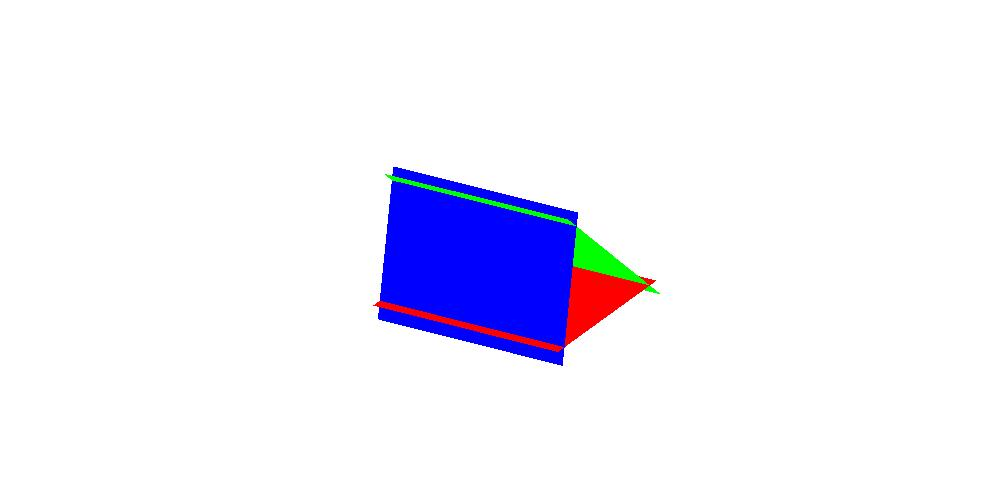
\includegraphics[scale=0.5,clip=true,
      trim=10cm 4.5cm 10cm 5.5cm]{images/toblerone}
 \]

\end{example}

\begin{example}\label{eg-lineq-ii}
 We will solve the equations
 \begin{align*}
  a + b + c + d &= 4 \\
  a + b - c - d &= 0 \\
  a - b + c - d &= 0 \\
  a - b - c + d &= 0.
 \end{align*}
 The corresponding augmented matrix can be row-reduced as follows:
 \[
  \left[\begin{array}{cccc|c}
    1 &  1 &  1 &  1 & 4 \\
    1 &  1 & -1 & -1 & 0 \\
    1 & -1 &  1 & -1 & 0 \\
    1 & -1 & -1 &  1 & 0
  \end{array}\right]
  \xra{1}
  \left[\begin{array}{cccc|c}
    1 &  1 &  1 &  1 &  4 \\
    0 &  0 & -2 & -2 & -4 \\
    1 & -1 &  1 & -1 & 0 \\
    0 &  0 & -2 &  2 & 0
  \end{array}\right]
  \xra{2}
  \left[\begin{array}{cccc|c}
    1 &  1 &  1 &  1 &  4 \\
    0 &  0 &  1 &  1 &  2 \\
    1 & -1 &  1 & -1 & 0 \\
    0 &  0 &  1 & -1 & 0
  \end{array}\right]
  \xra{3}
 \] \[
  \left[\begin{array}{cccc|c}
    1 &  1 &  0 &  0 & 2 \\
    0 &  0 &  1 &  1 & 2 \\
    1 & -1 &  0 &  0 & 0 \\
    0 &  0 &  1 & -1 & 0
  \end{array}\right]
  \xra{4}
  \left[\begin{array}{cccc|c}
    1 &  1 &  0 &  0 & 2 \\
    0 &  0 &  1 &  1 & 2 \\
    0 & -2 &  0 &  0 & -2 \\
    0 &  0 &  0 & -2 & -2
  \end{array}\right]
  \xra{5}
  \left[\begin{array}{cccc|c}
    1 &  1 &  0 &  0 & 2 \\
    0 &  0 &  1 &  1 & 2 \\
    0 &  1 &  0 &  0 & 1 \\
    0 &  0 &  0 &  1 & 1
  \end{array}\right]
  \xra{6}
 \] \[
  \left[\begin{array}{cccc|c}
    1 &  0 &  0 &  0 & 1 \\
    0 &  0 &  1 &  0 & 1 \\
    0 &  1 &  0 &  0 & 1 \\
    0 &  0 &  0 &  1 & 1
  \end{array}\right]
  \xra{7}
  \left[\begin{array}{cccc|c}
    1 &  0 &  0 &  0 & 1 \\
    0 &  1 &  0 &  0 & 1 \\
    0 &  0 &  1 &  0 & 1 \\
    0 &  0 &  0 &  1 & 1
  \end{array}\right]
 \]
 Here, rather than slavishly following Method~\ref{meth-RREF}, we have
 applied row operations in a more creative order to make the structure
 of the equations clearer.  The stages are as follows:
 \begin{itemize}
  \item[1] We subtract the first row from the second, and the third
   from the fourth.
  \item[2] We multiply the second and fourth rows by $-1/2$.
  \item[3] We subtract the second row from the first, and the fourth
   from the third.
  \item[4] We subtract the first row from the third, and the second
   from the fourth.
  \item[5] We multiply the third and fourth rows by $-1/2$.
  \item[6] We subtract the third row from the first, and the fourth
   from the second.
  \item[7] We exchange the second and third rows.
 \end{itemize}
 The final matrix corresponds to the equations $a=1$, $b=1$, $c=1$ and
 $d=1$, which give the unique solution to the original system of
 equations.
\end{example}

\begin{remark}
 Often we want to solve a \dfn{homogeneous} equation $Ax=0$, where
 the right hand side is zero.  This means that the relevant augmented
 matrix is $[A|0]$.  Row operations will not change the fact that the last
 column is zero, so the RREF of $[A|0]$ will just be $[A'|0]$, where
 $A'$ is the RREF of $A$.  In this context we can save writing by
 leaving out the extra column and just working with $A$.
\end{remark}
\begin{example}\label{eg-homogeneous}
 Consider the homogeneous system
 \begin{align*}
  a+b+c+d+e+f &= 0 \\
  2a+2b+2c+2d-e-f &= 0 \\
  3a+3b-c-d-e-f &= 0
 \end{align*}
 The corresponding unaugmented matrix can be row-reduced as follows:
 \[
  \bbm
    1 &  1 &  1 &  1 &  1 &  1 \\
    2 &  2 &  2 &  2 & -1 & -1 \\
    3 &  3 & -1 & -1 & -1 & -1
  \ebm \to \bbm
    1 &  1 &  0 &  0 &  0 &  0 \\
    0 &  0 &  1 &  1 &  0 &  0 \\
    0 &  0 &  0 &  0 &  1 &  1 
  \ebm
 \]
 (details are left to the reader).  The final matrix corresponds to
 the homogeneous system
 \[ a+b = 0 \hspace{5em} c+d=0 \hspace{5em} e+f=0. \]
 There are pivots in columns $1$, $3$ and $5$, meaning that $a$, $c$
 and $e$ are dependent variables, and $b$, $d$ and $f$ are
 independent.  After moving the independent variables to the right
 hand side, the solution becomes $a=-b$, $c=-d$ and $e=-f$.  If we
 prefer we can introduce new variables $\lm$, $\mu$ and $\nu$, and say
 that the general solution is
 \begin{align*}
  a &= -\lm & c &= -\mu & e &= -\nu \\
  b &=  \lm & d &=  \mu & f &=  \nu
 \end{align*}
 for arbitrary values of $\lm$, $\mu$ and $\nu$.
\end{example}

\section{Linear combinations}
\label{sec-lin-comb}

\begin{definition}\label{defn-lincomb}
 Let $v_1,\dotsc,v_k$ and $w$ be vectors in $\R^n$.  We say that $w$
 is a \dfn{linear combination} of $v_1,\dotsc,v_k$ if there exist
 scalars $\lm_1,\dots,\lm_k$ such that
 \[ w = \lm_1v_1 + \dotsb + \lm_kv_k. \]
\end{definition}

\begin{example}\label{eg-lincomb-i}
 Consider the following vectors in $\R^4$:
 \[ v_1 = \bbm 1 \\ -1 \\ 0 \\ 0 \ebm \hspace{3em}
    v_2 = \bbm 0 \\ 1 \\ -1 \\ 0 \ebm \hspace{3em}
    v_3 = \bbm 0 \\ 0 \\ 1 \\ -1 \ebm \hspace{3em}
    w   = \bbm 1 \\ 10 \\ 100 \\ -111 \ebm
 \]
 If we take $\lm_1=1$ and $\lm_2=11$ and $\lm_3=111$ we get
 \[ \lm_1 v_1 + \lm_2 v_2 + \lm_3 v_3 =
     \bbm 1 \\ -1 \\ 0 \\ 0 \ebm +
     \bbm 0 \\ 11 \\ -11 \\ 0 \ebm +
     \bbm 0 \\ 0 \\ 111 \\ -111 \ebm =
     \bbm 1 \\ 10 \\ 100 \\ -111 \ebm = w,
 \]
 which shows that $w$ is a linear combination of $v_1$, $v_2$ and
 $v_3$.
\end{example}

\begin{example}\label{eg-lincomb-ii}
 Consider the following vectors in $\R^4$:
 \[ v_1 = \bbm 0 \\ 1 \\  2 \\  3 \ebm \hspace{3em}
    v_2 = \bbm 0 \\ 1 \\  4 \\  9 \ebm \hspace{3em}
    v_3 = \bbm 0 \\ 1 \\  8 \\ 27 \ebm \hspace{3em}
    v_4 = \bbm 0 \\ 1 \\ 16 \\ 81 \ebm \hspace{3em}
    w = \bbm 1 \\ 1 \\ 1 \\ 1 \ebm.
 \]
 Any linear combination of $v_1,\dotsc,v_4$ has the form
 \[ \lm_1v_1 + \lm_2v_2 + \lm_3v_3 + \lm_4v_4 =
     \bbm 0 \\ \lm_1+\lm_2+\lm_3+\lm_4 \\
          2\lm_1+4\lm_2+8\lm_3+16\lm_4 \\
          3\lm_1+9\lm_2+27\lm_3+81\lm_4 \ebm.
 \]
 In particular, the first component of any such linear combination is
 zero.  (You should be able to see this without needing to write out
 the whole formula.)  As the first component of $w$ is not zero, we
 see that $w$ is \emph{not} a linear combination of $v_1,\dotsc,v_4$.
\end{example}

\begin{example}\label{eg-lincomb-iii}
 Consider the following vectors in $\R^3$:
 \[ v_1 = \bbm 1 \\ 1 \\ 1 \ebm \hspace{3em}
    v_2 = \bbm 1 \\ 2 \\ 1 \ebm \hspace{3em}
    v_3 = \bbm 1 \\ 3 \\ 1 \ebm \hspace{3em}
    v_4 = \bbm 1 \\ 4 \\ 1 \ebm \hspace{3em}
    v_5 = \bbm 1 \\ 5 \\ 1 \ebm \hspace{3em}
    w   = \bbm -1 \\ 0 \\ 1 \ebm.
 \]
 Any linear combination of $v_1,\dotsc,v_5$ has the form
 \[ \lm_1v_1 + \dotsb + \lm_5v_5 =
     \bbm \lm_1+\lm_2+\lm_3+\lm_4+\lm_5 \\
          \lm_1+2\lm_2+3\lm_3+4\lm_4+5\lm_5 \\
          \lm_1+\lm_2+\lm_3+\lm_4+\lm_5 \ebm.
 \]
 In particular, the first and last components of any such linear
 combination are the same.  Again, you should be able to see this
 without writing the full formula.  As the first and last components
 of $w$ are different, we see that $w$ is not a linear combination of
 $v_1,\dotsc,v_5$.
\end{example}
\begin{example}\label{eg-lincomb-iv}
 Let $v_1$, $v_2$ and $w$ be vectors in $\R^3$ (so we can think about
 them geometrically).  For simplicity, assume that all three vectors
 are nonzero, and that $v_1$ and $v_2$ do not point in the same
 direction, nor do they point in opposite directions.  This will mean
 that there is a unique plane $P$ that passes through $v_1$, $v_2$ and
 the origin.  It is not hard to see that $P$ is just the set of all
 possible linear combinations of $v_1$ and $v_2$.  Thus, our vector
 $w$ is a linear combination of $v_1$ and $v_2$ if and only if $w$
 lies in the plane $P$.
 \[ 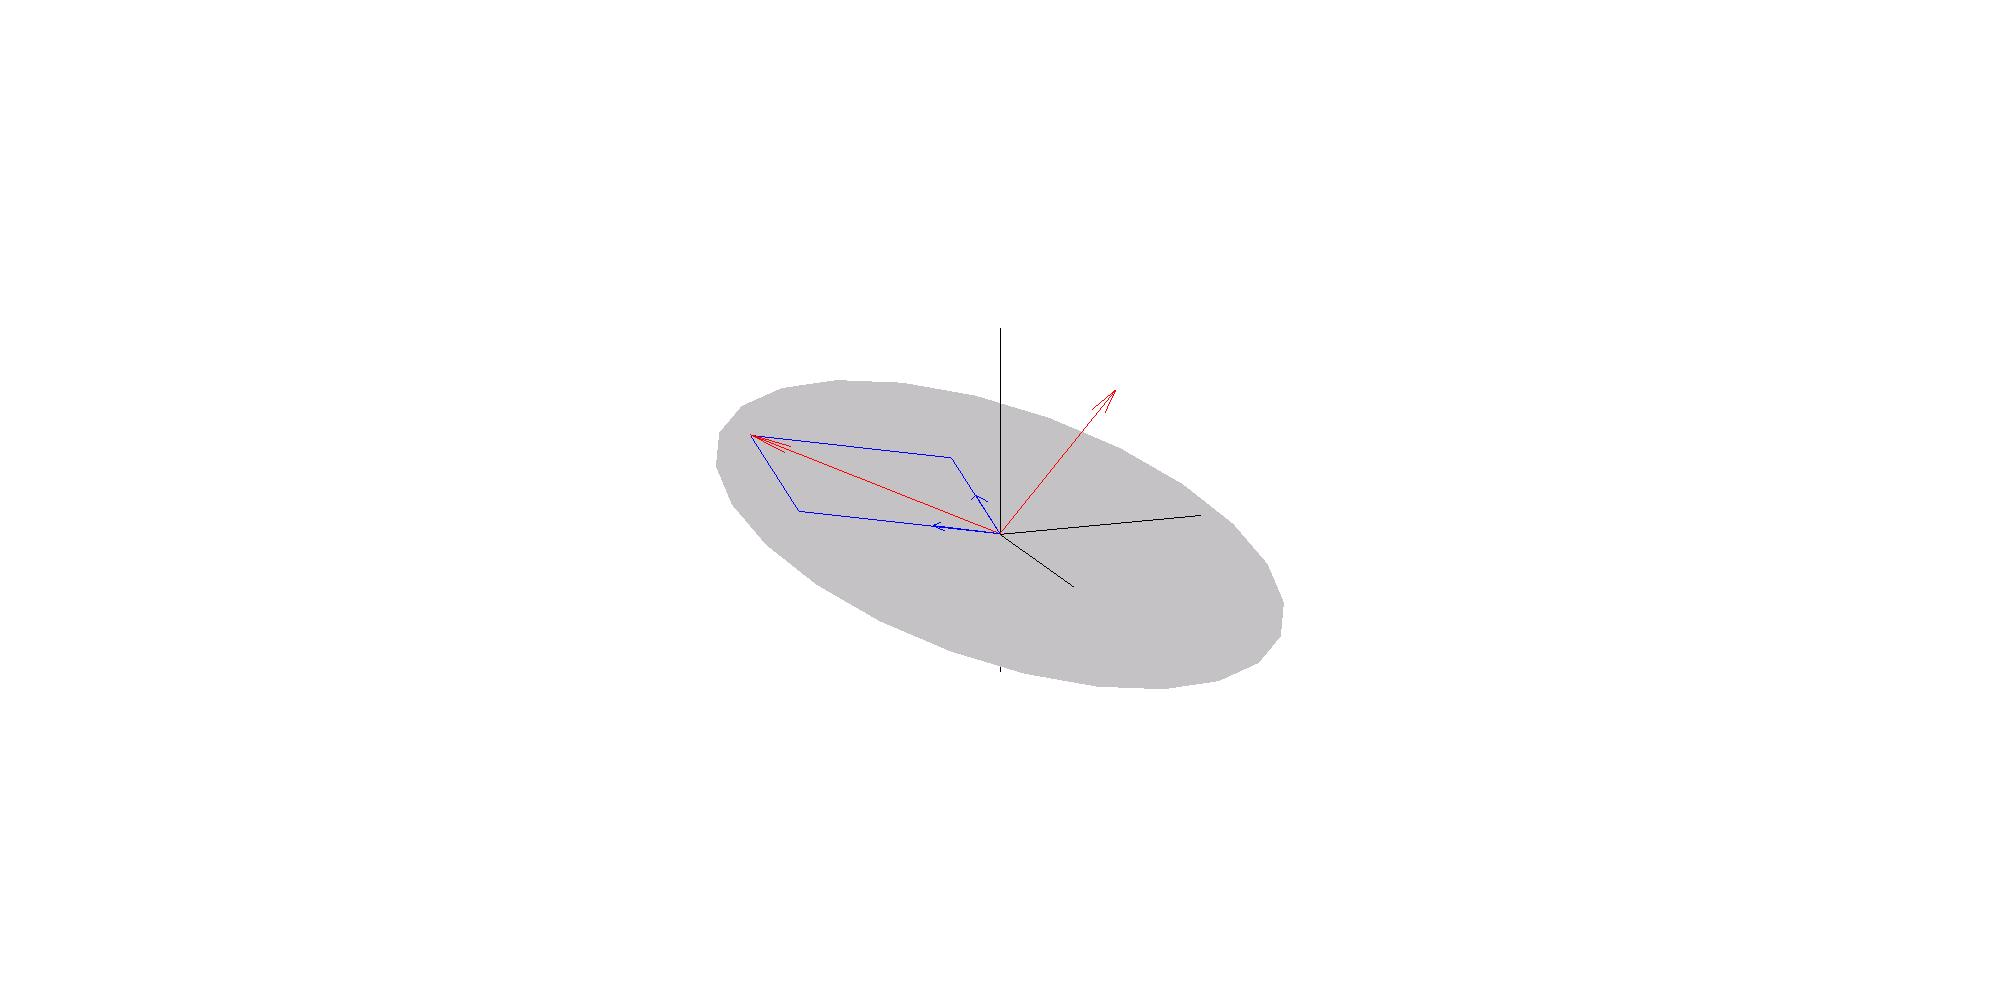
\includegraphics[scale=0.4,clip=true,
      trim=20cm 9cm 20cm 11cm]{images/plane_span}
 \]
\end{example}

We now want to explain a more systematic way to check whether a given
vector is a linear combination of some given list of vectors.
Note that for any $k$-vector
$\lm=\bbm\lm_1 & \dotsb & \lm_k\ebm^T$ we have
\[ A\lm =
    \left[\begin{array}{c|c|c}
     v_1 & \cdots & v_k
    \end{array}\right]
    \bbm \lm_1 \\ \vdots \\ \lm_k \ebm =
    \lm_1 v_1 + \dotsb + \lm_k v_k,
\]
which is the general form for a linear combination of
$v_1,\dotsc,v_k$.  This makes it clear that $w$ is a linear
combination of $v_1,\dotsc,v_k$ if and only if there is a vector $\lm$
which solves the matrix equation $A\lm=w$.  Using
Theorem~\ref{thm-row-ops} we see that the equation $A\lm=w$ has the
same solutions as the equation $A'\lm=w'$, which can be solved easily
by Method~\ref{meth-RREF-solve}.  We thus arrive at the following
method: 

\begin{method}\label{meth-find-lincomb}
 \index{linear combination}
 Suppose we have vectors $v_1,\dotsc,v_k\in\R^n$ and another vector
 $w\in\R^n$, and we want to express $w$ as a linear combination of the
 $v_i$ (or show that this is not possible).
 \begin{itemize}
  \item[(a)] We first let $A$ be the matrix whose columns are the
   vectors $v_i$:
   \[ A = \left[\begin{array}{c|c|c}
       v_1 & \cdots & v_k
      \end{array}\right] \in M_{n\tm k}(\R).
   \]
  \item[(b)] We then append $w$ as an additional column to get an
   augmented matrix
   \[ B  = \left[\begin{array}{c|c|c|c}
       v_1 & \cdots & v_k & w
      \end{array}\right]
       = \left[\begin{array}{c|c} A & w\end{array}\right].
   \]
   This corresponds to the matrix equation $A\lm=w$.
  \item[(c)] Row-reduce $B$ by Method~\ref{meth-RREF} to get a matrix
   $B'=[A'|w']$ in RREF.
  \item[(d)] If $B'$ has a pivot in the last column, then $w$ is not a
   linear combination of the vectors $v_1,\dotsc,v_k$.
  \item[(e)] If $B'$ has no pivot in the last column, then we can use
   Method~\ref{meth-RREF-solve} to find a vector
   $\lm=\bbm\lm_1 & \cdots & \lm_k\ebm^T$ satisfying $A'\lm=w'$.  We
   then have $A\lm=w$ and $\lm_1v_1+\dotsb+\lm_kv_k=w$, showing that
   $w$ is a linear combination of $v_1,\dotsc,v_k$.
 \end{itemize}
\end{method}

\begin{example}\label{eg-find-lincomb-i}
 Consider the vectors
 \[ v_1 = \bbm 11 \\ 11 \\ 1 \\ 1 \ebm \hspace{3em}
    v_2 = \bbm 1 \\ 11 \\ 11 \\ 1 \ebm \hspace{3em}
    v_3 = \bbm 1 \\ 1 \\ 11 \\ 11 \ebm \hspace{3em}
    w   = \bbm 121 \\ 221 \\ 1211 \\ 1111 \ebm.
 \]
 We ask whether $w$ can be expressed as a linear combination
 $w=\lm_1v_1+\lm_2v_2+\lm_3v_3$, and if so, what are the relevant
 values $\lm_1$, $\lm_2$ and $\lm_3$?  Following
 Method~\ref{meth-find-lincomb}, we write down the augmented
 matrix $[v_1|v_2|v_3|w]$ and row-reduce it:
 \[
  \left[\begin{array}{ccc|c}
   11 &  1 &  1 & 121 \\
   11 & 11 &  1 & 221 \\
    1 & 11 & 11 & 1211 \\
    1 &  1 & 11 & 1111
  \end{array}\right]
  \xra{1}
  \left[\begin{array}{ccc|c}
    1 &  1 & 11 & 1111 \\
   11 &  1 &  1 & 121 \\
   11 & 11 &  1 & 221 \\
    1 & 11 & 11 & 1211
  \end{array}\right]
  \xra{2}
  \left[\begin{array}{ccc|c}
    1 &   1 &   11 & 1111 \\
    0 & -10 & -120 & -12100 \\
    0 &   0 & -120 & -12000 \\
    0 &  10 &    0 & 100
  \end{array}\right]
  \xra{3}
 \] \[
  \left[\begin{array}{ccc|c}
    1 &   1 &   11 & 1111 \\
    0 &   1 &   12 & 1210 \\
    0 &   0 &    1 & 100 \\
    0 &   1 &    0 & 10
  \end{array}\right]
  \xra{4}
  \left[\begin{array}{ccc|c}
    1 &   1 &    0 & 11 \\
    0 &   1 &    0 & 10 \\
    0 &   0 &    1 & 100 \\
    0 &   1 &    0 & 10
  \end{array}\right]
  \xra{5}
  \left[\begin{array}{ccc|c}
    1 &   0 &    0 & 1 \\
    0 &   1 &    0 & 10 \\
    0 &   0 &    1 & 100 \\
    0 &   0 &    0 & 0
  \end{array}\right]
 \]
 (1: move the bottom row to the top; 2: subtract multiples of row 1
 from the other rows; 3: divide rows 2,3 and 4 by $-10$, $-120$ and
 $10$; 4: subtract multiples of row 3 from the other rows; 5: subtract
 multiples of row 2 from the other rows.)

 The final matrix corresponds to the system of equations
 \[ \lm_1 = 1 \hspace{3em}
    \lm_2 = 10 \hspace{3em}
    \lm_3 = 100 \hspace{3em}
     0 = 0
 \]
 so we conclude that
 \[ w = v_1 + 10 v_2 + 100 v_3. \]
 In particular, $w$ can be expressed as a linear combination of $v_1$,
 $v_2$ and $v_3$.  We can check the above equation directly:
 \[ v_1 + 10 v_2 + 100 v_3 =
      \bbm  11 \\  11 \\    1 \\    1 \ebm +
      \bbm  10 \\ 110 \\  110 \\   10 \ebm +
      \bbm 100 \\ 100 \\ 1100 \\ 1100 \ebm
    = \bbm 121 \\ 221 \\ 1211 \\ 1111 \ebm = w.
 \]
\end{example}

\begin{example}\label{eg-find-lincomb-ii}
 Consider the vectors
 \[ a_1 = \bbm 2 \\ -1 \\  0 \ebm \hspace{3em}
    a_2 = \bbm 3 \\  0 \\ -1 \ebm \hspace{3em}
    a_3 = \bbm 0 \\  3 \\ -2 \ebm \hspace{3em}
    b = \bbm 1 \\ 2 \\ 3 \ebm
 \]
 To test whether $b$ is a linear combination of $a_1$, $a_2$ and
 $a_3$, we write down the relevant augmented matrix and row-reduce it:
 \[
  \left[\begin{array}{ccc|c}
    2 &  3 &  0 & 1 \\
   -1 &  0 &  3 & 2 \\
    0 & -1 & -2 & 3
  \end{array}\right]
  \xra{1}
  \left[\begin{array}{ccc|c}
    1 &  0 & -3 & -2 \\
    0 &  1 &  2 & -3 \\
    2 &  3 &  0 &  1
  \end{array}\right]
  \xra{2}
  \left[\begin{array}{ccc|c}
    1 &  0 & -3 & -2 \\
    0 &  1 &  2 & -3 \\
    0 &  3 &  6 &  5
  \end{array}\right]
  \xra{3}
 \] \[
  \left[\begin{array}{ccc|c}
    1 &  0 & -3 & -2 \\
    0 &  1 &  2 & -3 \\
    0 &  0 &  0 & 14
  \end{array}\right]
  \xra{4}
  \left[\begin{array}{ccc|c}
    1 &  0 & -3 & -2 \\
    0 &  1 &  2 & -3 \\
    0 &  0 &  0 &  1
  \end{array}\right]
  \xra{5}
  \left[\begin{array}{ccc|c}
    1 &  0 & -3 &  0 \\
    0 &  1 &  2 &  0 \\
    0 &  0 &  0 &  1
  \end{array}\right]
 \]
 (Stage 1: move the top row to the bottom, and multiply the other two rows
 by $-1$; Stage 2: subtract $2$ times row 1 from row 3; Stage 3:
 subtract $3$ times row 2 from row 3; Stage 4: divide row 3 by $14$;
 Stage 5: subtract multiples of row 3 from rows 1 and 2.)

 The last matrix has a pivot in the rightmost column, corresponding to
 the equation $0=1$.  This means that the equation
 $\lm_1a_1+\lm_2a_2+\lm_3a_3=b$ cannot be solved for $\lm_1$, $\lm_2$
 and $\lm_3$, or in other words that $b$ is not a linear combination
 of $a_1$, $a_2$ and $a_3$.

 We can also see this in a more direct but less systematic way, as
 follows.  It is easy to check that $b.a_1=b.a_2=b.a_3=0$, which means
 that $b.(\lm_1a_1+\lm_2a_2+\lm_3a_3)=0$ for all possible choices of
 $\lm_1$, $\lm_2$ and $\lm_3$.  However, $b.b=14>0$, so $b$ cannot be
 equal to $\lm_1a_1+\lm_2a_2+\lm_3a_3$.
\end{example}

\section{Linear independence}

\begin{definition}\label{defn-dependent}
 Let $\CV=v_1,\dotsc,v_k$ be a list of vectors in $\R^n$.  A
 \dfn{linear relation} between the vectors $v_i$ is a relation of the
 form $\lm_1v_1+\dotsb+\lm_kv_k=0$, where $\lm_1,\dotsc,\lm_k$ are
 scalars.  In other words, it is a way of expressing $0$ as a linear
 combination of $\CV$.

 For any list we have the trivial linear relation
 $0v_1+0v_2+\dotsb+0v_k=0$.  There may or may not be any nontrivial
 linear relations.

 If the list $\CV$ has a nontrivial linear relation, we say that it is
 a \dfn{linearly dependent} list.  If the only linear relation on
 $\CV$ is the trivial one, we instead say that $\CV$ is \dfn{linearly
  independent}.  We will often omit the word ``linearly'' for the sake
 of brevity.
\end{definition}

\begin{example}\label{eg-dep-i}
 Consider the list $\CV$ given by
 \[ v_1 = \bbm 1 \\ 1 \\ 0 \\ 0 \ebm \hspace{3em}
    v_2 = \bbm 0 \\ 0 \\ 1 \\ 1 \ebm \hspace{3em}
    v_3 = \bbm 1 \\ 0 \\ 0 \\ 1 \ebm \hspace{3em}
    v_4 = \bbm 0 \\ 1 \\ 1 \\ 0 \ebm.
 \]
 There is a nontrivial linear relation $v_1+v_2-v_3-v_4=0$, so the
 list $\CV$ is dependent.
\end{example}
\begin{example}\label{eg-dep-ii}
 Consider the list $\CA$ given by
 \[ a_1 = \bbm  1 \\  2 \ebm \hspace{3em}
    a_2 = \bbm 12 \\  1 \ebm \hspace{3em}
    a_3 = \bbm -1 \\ -1 \ebm \hspace{3em}
    a_4 = \bbm  3 \\  1 \ebm.
 \]
 Just by writing it out, you can check that
 \[ 3a_1 + a_2 + 3a_3 -4a_4 = 0. \]
 \begin{center}
  \begin{tikzpicture}[scale=0.3]
   \fill( 0,0) circle(0.1);
   \fill( 3,6) circle(0.1);
   \fill(15,7) circle(0.1);
   \fill(12,4) circle(0.1);
   \draw[->, shorten >= 1pt] (0,0) -- (3,6);
   \draw[->, shorten >= 1pt] (3,6) -- (15,7);
   \draw[->, shorten >= 1pt] (15,7) -- (12,4);
   \draw[->, shorten >= 1pt] (12,4) -- (0,0);
   \draw ( 1.5,3.0) node[anchor=south east]{$\ss 3a_1$};
   \draw ( 9.0,6.5) node[anchor=south]{$\ss a_2$};
   \draw (13.5,5.5) node[anchor=north west]{$\ss 3a_3$};
   \draw ( 6.0,2.0) node[anchor=north]{$\ss -4a_4$};
  \end{tikzpicture}
 \end{center}
 This is a nontrivial linear relation on the list $\CA$, so $\CA$ is
 dependent.
\end{example}
\begin{example}\label{eg-indep-i}
 Consider the list $\CU$ given by
 \[ u_1 = \bbm 1 \\ 1 \\ 0 \\ 0 \ebm \hspace{3em}
    u_2 = \bbm 0 \\ 1 \\ 1 \\ 0 \ebm \hspace{3em}
    u_3 = \bbm 0 \\ 0 \\ 1 \\ 1 \ebm.
 \]
 We claim that this is independent.  To see this, consider a linear
 relation $\lm_1u_1+\lm_2u_2+\lm_3u_3=0$.  Writing this out, we get
 \[ \bbm \lm_1 \\ \lm_1+\lm_2 \\ \lm_2+\lm_3 \\ \lm_3 \ebm =
    \bbm 0 \\ 0 \\ 0 \\ 0 \ebm.
 \]
 By looking at the first and last rows we see that $\lm_1=\lm_3=0$.
 By looking at the second row we get $\lm_2=-\lm_1=0$ as well so our
 relation is the trivial relation.  As the only linear relation is the
 trivial one, we see that $\CU$ is independent.
\end{example}

\begin{lemma}\label{lem-multiples}
 Let $v$ and $w$ be vectors in $\R^n$, and suppose that $v\neq 0$ and
 that the list $(v,w)$ is linearly dependent.  Then there is a number
 $\al$ such that $w=\al v$.
\end{lemma}
\begin{proof}
 Because the list is dependent, there is a linear relation
 $\lm v+\mu w=0$ where $\lm$ and $\mu$ are not both zero.  There are
 apparently three possibilities: (a) $\lm\neq 0$ and $\mu\neq 0$; (b)
 $\lm=0$ and $\mu\neq 0$; (c) $\lm\neq 0$ and $\mu=0$.  However,
 case~(c) is not really possible.  Indeed, in case~(c) the equation
 $\lm v+\mu w=0$ would reduce to $\lm v=0$, and we could multiply by
 $\lm^{-1}$ to get $v=0$; but $v\neq 0$ by assumption.  In case~(a)
 or~(b) we can take $\al=-\lm/\mu$ and we have $w=\al v$.
\end{proof}

There is a systematic method using row-reduction for checking linear
(in)dependence, as we will explain shortly.  We first need a
preparatory observation.

\begin{definition}\label{defn-wide}
 Let $B$ be a $p\tm q$ matrix.  We say that $B$ is \dfn{wide} if
 $p<q$, or \dfn{square} if $p=q$ or \dfn{tall} if $p>q$.
 \[ \begin{array}{ccccc}
     \bbm 1 & 2 & 3 \\ 4 & 5 & 6 \ebm & &
     \bbm 1 & 2 & 1 \\ 2 & 3 & 2 \\ 1 & 2 & 1 \ebm & &
     \bbm 1 & 1 \\ 0 & 0 \\ 1 & 1 \ebm \\
     \text{ wide } & & \text{ square } & & \text{ tall }
    \end{array}
 \]
\end{definition}
\begin{lemma}\label{lem-pivots-everywhere}
 \index{pivot}
 Let $B$ be a $p\tm q$ matrix in RREF.
 \begin{itemize}
  \item[(a)] If $B$ is wide then it is impossible for every column to
   contain a pivot.
  \item[(b)] If $B$ is square then the only way for every column to
   contain a pivot is if $B=I_q$.
  \item[(c)] If $B$ is tall  then the only way for every column to
   contain a pivot is if $B$ consists of $I_q$ with $(p-q)$ rows of
   zeros added at the bottom (so
   $B=\left[\begin{array}{c} I_q \\ \hline 0_{(p-q)\tm q}
      \end{array}\right]$).
 \end{itemize}
\end{lemma}

For example, the only $5\tm 3$ RREF matrix with a pivot in every
column is this one:
\[ \left[\begin{array}{c}
      I_3 \\ \hline 0_{2\tm 3} 
   \end{array}\right] =
   \left[\begin{array}{ccc}
    1 & 0 & 0 \\
    0 & 1 & 0 \\
    0 & 0 & 1 \\ \hline
    0 & 0 & 0 \\
    0 & 0 & 0
   \end{array}\right]
\]

\begin{proof}
 There is at most one pivot in every row, making at most $p$ pivots
 altogether.  If $B$ is wide then we have $q$ columns with $q>p$, so
 there are not enough pivots to have one in every column.  This
 proves~(a).

 Now suppose instead that $B$ does have a pivot in every column, so
 there are $q$ pivots and we must have $p\geq q$.  As $B$ is in RREF
 we know that all entries above or below a pivot are zero.  As there
 is a pivot in every column it follows that the pivots are the only
 nonzero entries in $B$.  Every nonzero row contains precisely one
 pivot, so there must be $q$ nonzero rows.  The remaining $(p-q)$ rows
 are all zero, and they must occur at the bottom of $B$ (because $B$
 is in RREF).  Now the top $q\tm q$ block contains $q$ pivots which
 move to the right as we go down the matrix.  It is easy to see that
 the only possibility for the top block is $I_q$, which proves~(b)
 and~(c).
\end{proof}

\begin{method}\label{meth-check-dependence}
 \index{linearly dependent}\index{linearly independent}\index{pivot}
 Let $\CV=v_1,\dotsc,v_m$ be a list of vectors in $\R^n$.  We can
 check whether this list is dependent as follows.
 \begin{itemize}
  \item[(a)] Form the $n\tm m$ matrix
   \[ A = \left[\begin{array}{c|c|c}
              && \\
              v_1 & \dotsc & v_m \\
              &&
            \end{array}\right]
   \]
   whose columns are the vectors $v_i$.
  \item[(b)] Row reduce $A$ to get another $n\tm m$ matrix $B$ in
   RREF.
  \item[(c)] If every column of $B$ contains a pivot (so $B$ has the
   form discussed in Lemma~\ref{lem-pivots-everywhere}) then $\CV$ is
   independent.
  \item[(d)] If some column of $B$ has no pivot, then the list $\CV$
   is dependent.  Moreover, we can find the coefficients $\lm_i$ in a
   nontrivial linear relation by solving the vector equation $B\lm=0$
   (which is easy because $B$ is in RREF).
 \end{itemize}
\end{method}
\begin{remark}\label{rem-dependence-shortcut}
 \index{wide}\index{numerical criteria}
 If $m>n$ then $\CV$ is automatically dependent and we do not need to
 go through the method.  (For example, any list of $5$ vectors in
 $\R^3$ is automatically dependent, any list of $10$ vectors in $\R^9$
 is automatically dependent, and so on.)  Indeed, in this case the
 matrices $A$ and $B$ are wide, so it is impossible for $B$ to have a
 pivot in every column.  However, this line of argument only tells us
 that there \textbf{exists} a nontrivial relation
 $\lm_1v_1+\dotsb+\lm_mv_m=0$, it does not tell us the coefficients
 $\lm_i$.  If we want to find the $\lm_i$ then we do need to go
 through the whole method as explained above.
\end{remark}

We will give some examples of using the above method, and then explain
why the method is correct.

\begin{example}\label{eg-dep-i-matrix}
 In example~\ref{eg-dep-i} we considered the list
 \[ v_1 = \bbm 1 \\ 1 \\ 0 \\ 0 \ebm \hspace{3em}
    v_2 = \bbm 0 \\ 0 \\ 1 \\ 1 \ebm \hspace{3em}
    v_3 = \bbm 1 \\ 0 \\ 0 \\ 1 \ebm \hspace{3em}
    v_4 = \bbm 0 \\ 1 \\ 1 \\ 0 \ebm.
 \]
 We can write down the corresponding matrix and row-reduce it as
 follows:
 \[
  \bbm 1 & 0 & 1 & 0 \\
       1 & 0 & 0 & 1 \\
       0 & 1 & 0 & 1 \\
       0 & 1 & 1 & 0
  \ebm \xra{1}
  \bbm 1 & 0 & 1 & 0 \\
       0 & 0 &-1 & 1 \\
       0 & 1 & 0 & 1 \\
       0 & 0 & 1 &-1
  \ebm \xra{2}
  \bbm 1 & 0 & 1 & 0 \\
       0 & 1 & 0 & 1 \\
       0 & 0 & 1 &-1 \\
       0 & 0 &-1 & 1
  \ebm \xra{3}
  \bbm 1 & 0 & 0 & 1 \\
       0 & 1 & 0 & 1 \\
       0 & 0 & 1 &-1 \\
       0 & 0 & 0 & 0
  \ebm
 \]
 The end result has no pivot in the last column, so the original list is
 dependent.  To find a specific linear relation, we solve the equation
 \[   \bbm 1 & 0 & 0 & 1 \\
           0 & 1 & 0 & 1 \\
           0 & 0 & 1 &-1 \\
           0 & 0 & 0 & 0
      \ebm
      \bbm \lm_1 \\ \lm_2 \\ \lm_3 \\ \lm_4 \ebm =
      \bbm 0 \\ 0 \\ 0 \\ 0 \ebm
 \]
 to get $\lm_1=-\lm_4$, $\lm_2=-\lm_4$ and $\lm_3=\lm_4$ with $\lm_4$
 arbitrary.  Taking $\lm_4=1$ gives
 $(\lm_1,\lm_2,\lm_3,\lm_4)=(-1,-1,1,1)$, corresponding to the
 relation $-v_1-v_2+v_3+v_4=0$.
\end{example}
\begin{example}\label{eg-dep-ii-matrix}
 In Example~\ref{eg-dep-ii} we considered the list
 \[ a_1 = \bbm  1 \\  2 \ebm \hspace{3em}
    a_2 = \bbm 12 \\  1 \ebm \hspace{3em}
    a_3 = \bbm -1 \\ -1 \ebm \hspace{3em}
    a_4 = \bbm  3 \\  1 \ebm.
 \]
 Here we have $4$ vectors in $\R^2$, so they must be dependent by
 Remark~\ref{rem-dependence-shortcut}.  Thus, there exist nontrivial
 linear relations
 \[ \lm_1a_1 + \lm_2a_2 + \lm_3a_3 + \lm_4a_4 = 0. \]
 To actually find such a relation, we write down the corresponding
 matrix and row-reduce it as follows:
 \[
  \bbm
   1 & 12 & -1 & 3 \\
   2 & 1  & -1 & 1
  \ebm
  \xra{}
  \bbm
   1 &  12 & -1 & 3 \\
   0 & -23 &  1 & -5
  \ebm
  \xra{}
  \bbm
   1 &  12 & -1 & 3 \\
   0 &  1 & -1/23 & 5/23
  \ebm
  \xra{}
  \bbm
   1 &  0 & -11/23 & 9/23 \\
   0 &  1 & -1/23 & 5/23
  \ebm
 \]
 We now need to solve the matrix equation
 \[ \bbm
     1 &  0 & -11/23 & 9/23 \\
     0 &  1 & -1/23 & 5/23
    \ebm
    \bbm \lm_1 \\ \lm_2 \\ \lm_3 \\ \lm_4 \ebm =
    \bbm 0 \\ 0 \ebm
 \]
 As this is in RREF, we can just read off the solution:
 $\lm_1=\frac{11}{23}\lm_3-\frac{9}{23}\lm_4$ and
 $\lm_2=\frac{1}{23}\lm_3-\frac{5}{23}\lm_4$
 with $\lm_3$ and $\lm_4$ arbitrary.  If we choose $\lm_3=23$ and
 $\lm_4=0$ we get $(\lm_1,\lm_2,\lm_3,\lm_4)=(11,1,23,0)$ so we have a
 relation
 \[ 11 a_1 + a_2 + 23 a_3 + 0 a_4 = 0. \]
 (You should check directly that this is correct.)  Alternatively, we
 can choose $\lm_3=3$ and $\lm_4=-4$.  Using the equations
 $\lm_1=\frac{11}{23}\lm_3-\frac{9}{23}\lm_4$ and
 $\lm_2=\frac{1}{23}\lm_3-\frac{5}{23}\lm_4$ we get $\lm_1=3$ and
 $\lm_2=1$ giving a different relation
 \[ 3a_1 + a_2 + 3a_3 - 4a_4 = 0. \]
 This is the relation that we observed in Example~\ref{eg-dep-ii}.
\end{example}
\begin{example}\label{eg-indep-i-matrix}
 In Example~\ref{eg-indep-i} we considered the list $\CU$ given by
 \[ u_1 = \bbm 1 \\ 1 \\ 0 \\ 0 \ebm \hspace{3em}
    u_2 = \bbm 0 \\ 1 \\ 1 \\ 0 \ebm \hspace{3em}
    u_3 = \bbm 0 \\ 0 \\ 1 \\ 1 \ebm.
 \]
 We can write down the corresponding matrix and row-reduce it as
 follows:
 \[
  \bbm
   1 & 0 & 0 \\
   1 & 1 & 0 \\
   0 & 1 & 1 \\
   0 & 0 & 1
  \ebm
  \to
  \bbm
   1 & 0 & 0 \\
   0 & 1 & 0 \\
   0 & 1 & 1 \\
   0 & 0 & 1
  \ebm
  \to
  \bbm
   1 & 0 & 0 \\
   0 & 1 & 0 \\
   0 & 0 & 1 \\
   0 & 0 & 1
  \ebm
  \to
  \left[\begin{array}{ccc}
   1 & 0 & 0 \\
   0 & 1 & 0 \\
   0 & 0 & 1 \\ \hline
   0 & 0 & 0
  \end{array}\right]
 \]
 The final matrix has a pivot in every column, as in
 Lemma~\ref{lem-pivots-everywhere}.  It follows that the list $\CU$ is
 independent.
\end{example}

\begin{proof}[Proof of correctness of Method~\ref{meth-check-dependence}]
 Put
 \[ A = \left[\begin{array}{c|c|c}
              && \\
              v_1 & \cdots & v_m \\
              &&
        \end{array}\right]
 \]
 as in step~(a) of the method, and let $B$ be the RREF form of $A$.
 Note that for any vector
 $\lm=\bbm \lm_1 & \dotsc & \lm_m\ebm^T\in\R^m$, we have
 \[ A\lm =
     \left[\begin{array}{c|c|c}
              && \\
              v_1 & \cdots & v_m \\
              &&
     \end{array}\right]
     \bbm \lm_1 \\ \vdots \\ \lm_m \ebm =
     \lm_1v_1 + \dotsb + \lm_mv_m.
 \]
 Thus, linear relations on our list are just the same as solutions to
 the homogeneous equation $A\lm=0$.  By Theorem~\ref{thm-row-ops},
 these are the same as solutions to the equation $B\lm=0$, which can
 be found by Method~\ref{meth-RREF-solve}.  If there is a pivot in
 every column then none of the variables $\lm_i$ is independent, so
 the only solution is $\lm_1=\lm_2=\dotsb=\lm_m=0$.  Thus, the only
 linear relation on $\CV$ is the trivial one, which means that the
 list $\CV$ is linearly independent.

 Suppose instead that some column (the $k$'th one, say) does not
 contain a pivot.  Then in Method~\ref{meth-RREF-solve} the variable
 $\lm_k$ will be independent, so we can choose $\lm_k=1$.  This will
 give us a nonzero solution to $B\lm=0$, or equivalently $A\lm=0$,
 corresponding to a nontrivial linear relation on $\CV$.  This shows
 that $\CV$ is linearly dependent.
\end{proof}

\section{Spanning sets}
\label{sec-spanning}

\begin{definition}\label{defn-spanning-list}
 Suppose we have a list $\CV=v_1,\dotsc,v_m$ of vectors in $\R^n$.  We
 say that the list \emph{spans}\index{span} $\R^n$ if \textbf{every} vector in
 $\R^n$ can be expressed as a linear combination of $v_1,\dotsc,v_m$.
\end{definition}
\begin{example}\label{eg-not-span-i}
 Consider the list $\CV=v_1,v_2,v_3,v_4$, where
 \[ v_1 = \bbm 0 \\ 1 \\  2 \\  3 \ebm \hspace{3em}
    v_2 = \bbm 0 \\ 1 \\  4 \\  9 \ebm \hspace{3em}
    v_3 = \bbm 0 \\ 1 \\  8 \\ 27 \ebm \hspace{3em}
    v_4 = \bbm 0 \\ 1 \\ 16 \\ 81 \ebm
 \]
 In Example~\ref{eg-lincomb-ii} we saw that the vector
 $w=\bbm 1 & 1 & 1 & 1\ebm^T$ is not a linear combination of this
 list, so the list $\CV$ does not span $\R^4$.
\end{example}
\begin{example}\label{eg-not-span-ii}
 Consider the list $\CV=v_1,v_2,v_3,v_4,v_5$, where
 \[ v_1 = \bbm 1 \\ 1 \\ 1 \ebm \hspace{3em}
    v_2 = \bbm 1 \\ 2 \\ 1 \ebm \hspace{3em}
    v_3 = \bbm 1 \\ 3 \\ 1 \ebm \hspace{3em}
    v_4 = \bbm 1 \\ 4 \\ 1 \ebm \hspace{3em}
    v_5 = \bbm 1 \\ 5 \\ 1 \ebm.
 \]
 In Example~\ref{eg-lincomb-iii} we saw that the vector
 $w=\bbm -1 & 0 & 1 \ebm^T$ is not a linear combination of this
 list, so the list $\CV$ does not span $\R^3$.
\end{example}
\begin{example}\label{eg-not-span-iii}
 Similarly, Example~\ref{eg-find-lincomb-ii} shows that the list
 \[ \CA = \bbm 2 \\ -1 \\  0 \ebm, \qquad
          \bbm 3 \\  0 \\ -1 \ebm, \qquad
          \bbm 0 \\  3 \\ -2 \ebm
 \]
 does not span $\R^3$.
\end{example}

\begin{example}\label{eg-span-i}
 Consider the list $\CU=u_1,u_2,u_3$, where
 \[ u_1 = \bbm 1 \\ 1 \\ 0 \ebm \hspace{3em}
    u_2 = \bbm 1 \\ 0 \\ 1 \ebm \hspace{3em}
    u_3 = \bbm 0 \\ 1 \\ 1 \ebm.
 \]
 We will show that these span $\R^3$.  Indeed, for any vector
 $v=\bbm x & y & z\ebm^T\in\R^3$ we can put
 \[ \lm_1 = \frac{ x+y-z}{2} \hspace{4em}
    \lm_2 = \frac{ x-y+z}{2} \hspace{4em}
    \lm_3 = \frac{-x+y+z}{2}
 \]
 and we find that
 \begin{align*}
  \lm_1u_1+\lm_2u_2+\lm_3u_3
    &=
   \bbm (x+y-z)/2 \\ (x+y-z)/2 \\ 0 \ebm +
   \bbm (x-y+z)/2 \\ 0 \\ (x-y+z)/2 \ebm +
   \bbm 0 \\ (-x+y+z)/2 \\ (-x+y+z)/2 \ebm \\
    &=
   \bbm (x+y-z+x-y+z)/2 \\
        (x+y-z-x+y+z)/2 \\
        (x-y+z-x+y+z)/2 \ebm
    = \bbm x \\ y \\ z \ebm = v.
 \end{align*}
 This expresses $v$ as a linear combination of the list $\CU$, as
 required.
\end{example}

\begin{example}\label{eg-span-ii}
 Consider the list $\CA=a_1,a_2,a_3$ where
 \[ a_1 = \bbm 1 \\ 2 \ebm \hspace{3em}
    a_2 = \bbm 2 \\ 3 \ebm \hspace{3em}
    a_3 = \bbm 3 \\ 5 \ebm.
 \]
 Let $v=\bbm x \\ y\ebm$ be an arbitrary vector in $\R^2$.  Just by
 expanding out the right hand side, we see that
 \[ \bbm x \\ y \ebm =
     (2y-4x)\bbm 1 \\ 2 \ebm + (x-y)\bbm 2\\ 3\ebm + x\bbm 3\\5 \ebm,
 \]
 or in other words
 \[ v = (2y-4x)a_1 + (x-y)a_2 + x a_3. \]
 This expresses an arbitrary vector $v\in\R^2$ as a linear combination
 of $a_1$, $a_2$ and $a_3$, proving that the list $\CA$ spans $\R^2$.

 In this case there are actually many different ways in which we can
 express $v$ as a linear combination of $a_1$, $a_2$ and $a_3$.
 Another one is
 \[ v = (y-3x)a_1 + (2x-2y)a_2 + y a_3. \]
\end{example}

We now discuss a systematic method for spanning problems.

\begin{method}\label{meth-check-span}
 \index{span}\index{pivot}
 Let $\CV=v_1,\dotsc,v_m$ be a list of vectors in $\R^n$.  We can
 check whether this list spans $\R^n$ as follows.
 \begin{itemize}
  \item[(a)] Form the $m\tm n$ matrix
   \[ \renewcommand{\arraystretch}{1.3}
       C = \left[\begin{array}{ccc}
              & v_1^T & \\ \hline
              & \vdots & \\ \hline
              & v_m^T &
            \end{array}\right]
   \]
   whose rows are the row vectors $v_i^T$.
  \item[(b)] Row reduce $C$ to get another $m\tm n$ matrix $D$ in
   RREF.
  \item[(c)] If every column of $D$ contains a pivot (so $D$ has the
   form discussed in Lemma~\ref{lem-pivots-everywhere}) then $\CV$
   spans $\R^n$.
  \item[(d)] If some column of $D$ has no pivot, then the list $\CV$
   does not span $\R^n$.
 \end{itemize}
\end{method}
\begin{remark}\label{rem-dual-methods}
 This is almost exactly the same as
 Method~\ref{meth-check-dependence}, except that here we start by
 building a matrix whose rows are $v_i^T$, whereas in
 Method~\ref{meth-check-dependence} we start by building a matrix
 whose columns are $v_i$.  Equivalently, the matrix $C$ in this method
 is the transpose of the matrix $A$ in
 Method~\ref{meth-check-dependence}.  Note, however, that transposing
 does not interact well with row-reduction, so the matrix $D$ is
 \textbf{not} the transpose of $B$.
\end{remark}
\begin{remark}\label{rem-spanning-shortcut}
 \index{wide}\index{numerical criteria}
 If $m<n$ then the matrices $C$ and $D$ above will be wide, so $D$
 cannot have a pivot in every column, so the list $\CV$ cannot span
 $\R^n$.  For example, no list of $4$ vectors can span $\R^6$, and any
 list that spans $\R^8$ must contain at least $8$ vectors and so on.
\end{remark}

We will give some examples of using this method, then explain why it
works.
\begin{example}\label{eg-not-span-i-matrix}
 Consider the list
 \[ v_1 = \bbm 0 \\ 1 \\  2 \\  3 \ebm \hspace{3em}
    v_2 = \bbm 0 \\ 1 \\  4 \\  9 \ebm \hspace{3em}
    v_3 = \bbm 0 \\ 1 \\  8 \\ 27 \ebm \hspace{3em}
    v_4 = \bbm 0 \\ 1 \\ 16 \\ 81 \ebm
 \]
 as in Example~\ref{eg-not-span-i} (so $n=m=4$).  The relevant matrix
 $C$ is
 \[ C   = \bbm
           0 & 1 &  2 &  3 \\
           0 & 1 &  4 &  9 \\
           0 & 1 &  8 & 27 \\
           0 & 1 & 16 & 81
          \ebm
 \]
 The first column is zero, and will remain zero no matter what row
 operations we perform.  Thus $C$ cannot reduce to the identity
 matrix, so $\CV$ does not span (as we already saw by a different
 method).  In fact the row-reduction is
 \[ C \to \bbm 0 & 1 & 0 & 0 \\
               0 & 0 & 1 & 0 \\
               0 & 0 & 0 & 1 \\
               0 & 0 & 0 & 0 \ebm
 \]
 but it is not really necessary to go through the whole calculation.
\end{example}
\begin{example}\label{eg-not-span-ii-matrix}
 Consider the list
 \[ v_1 = \bbm 1 \\ 1 \\ 1 \ebm \hspace{3em}
    v_2 = \bbm 1 \\ 2 \\ 1 \ebm \hspace{3em}
    v_3 = \bbm 1 \\ 3 \\ 1 \ebm \hspace{3em}
    v_4 = \bbm 1 \\ 4 \\ 1 \ebm \hspace{3em}
    v_5 = \bbm 1 \\ 5 \\ 1 \ebm.
 \]
 as in Example~\ref{eg-not-span-ii} (so $n=3$ and $m=5$).  The
 relevant row-reduction is
 \[
  \bbm 1 & 1 & 1 \\ 1 & 2 & 1 \\ 1 & 3 & 1 \\ 1 & 4 & 1 \\ 1 & 5 & 1 \ebm
  \to
  \bbm 1 & 1 & 1 \\ 0 & 1 & 0 \\ 0 & 2 & 0 \\ 0 & 3 & 0 \\ 0 & 4 & 0 \ebm
  \to
  \left[\begin{array}{ccc}
   1 & 0 & 1 \\
   0 & 1 & 0 \\
   0 & 0 & 0 \\ \hline
   0 & 0 & 0 \\
   0 & 0 & 0 
  \end{array}\right]
 \]
 At the end of the process the last column does not contain a pivot
 (so the top $3\tm 3$ block is not the identity),
 so the original list does not span.  Again, we saw this earlier by a
 different method.
\end{example}
\begin{example}
 For the list
 \[ \CA = \bbm 2 \\ -1 \\  0 \ebm, \qquad
          \bbm 3 \\  0 \\ -1 \ebm, \qquad
          \bbm 0 \\  3 \\ -2 \ebm
 \]
 in Example~\ref{eg-not-span-iii}, the relevant row-reduction is
 \[ \bbm 2 & -1 & 0 \\ 3 & 0 & -1 \\ 0 & 3 & -2 \ebm \to
    \bbm 1 & -\half & 0 \\ 3 & 0 & -1 \\ 0 & 3 & -2 \ebm \to
    \bbm 1 & -\half & 0 \\ 0 & \tfrac{3}{2} & -1 \\ 0 & 3 & -2 \ebm \to
    \bbm 1 & -\half & 0 \\ 0 & 1 & -\tfrac{2}{3} \\ 0 & 0 & 0 \ebm \to
    \bbm 1 & 0 & -\tfrac{1}{3} \\ 0 & 1 & -\tfrac{2}{3} \\ 0 & 0 & 0 \ebm.
 \]
 In the last matrix the third column has no pivot, so the list does
 not span.
\end{example}
\begin{example}\label{eg-span-i-matrix}
 Consider the list $\CU=u_1,u_2,u_3$ from Example~\ref{eg-span-i}.
 \[ u_1 = \bbm 1 \\ 1 \\ 0 \ebm \hspace{3em}
    u_2 = \bbm 1 \\ 0 \\ 1 \ebm \hspace{3em}
    u_3 = \bbm 0 \\ 1 \\ 1 \ebm.
 \]
 The relevant row-reduction is
 \[ \bbm 1 & 1 & 0 \\ 1 &  0 &  1 \\ 0 & 1 & 1 \ebm \to
    \bbm 1 & 1 & 0 \\ 0 & -1 &  1 \\ 0 & 1 & 1 \ebm \to
    \bbm 1 & 1 & 0 \\ 0 &  1 & -1 \\ 0 & 0 & 2 \ebm \to
    \bbm 1 & 1 & 0 \\ 0 &  1 &  0 \\ 0 & 0 & 1 \ebm \to
    \bbm 1 & 0 & 0 \\ 0 &  1 &  0 \\ 0 & 0 & 1 \ebm
 \]
 The end result is the identity matrix, so the list $\CU$ spans
 $\R^3$.
\end{example}
\begin{example}
 Consider the list $\CA=\bbm 1\\2\ebm,\;\bbm 2\\3\ebm,\;\bbm 3\\5\ebm$
 from Example~\ref{eg-span-ii}.  The relevant row-reduction is
 \[ \bbm 1 & 2 \\ 2 & 3 \\ 3 & 5 \ebm \to
    \bbm 1 & 2 \\ 0 & -1 \\ 0 & -1 \ebm \to
    \bbm 1 & 2 \\ 0 &  1 \\ 0 & -1 \ebm \to
    \left[\begin{array}{cc}
     1 & 0 \\ 0 &  1 \\ \hline 0 & 0 
    \end{array}\right]
 \]
 In the last matrix, the top $2\tm 2$ block is the identity.  This
 means that the list $\CA$ spans $\R^2$.
\end{example}

We now explain why Method~\ref{meth-check-span} is valid.
\begin{lemma}\label{lem-span-invariant}
 \index{span}
 Let $C$ be an $m\tm n$ matrix, and let $C'$ be obtained from $C$ by a
 single elementary row operation.  Let $s$ be a row vector of length
 $n$.  Then $s$ can be expressed as a linear combination of the rows
 of $C$ if and only if it can be expressed as a linear combination of
 the rows of $C'$.
\end{lemma}
\begin{proof}
 Let the rows of $C$ be $r_1,\dotsc,r_m$.  Suppose that $s$ is a
 linear combination of these rows, say
 \[ s=\lm_1r_1+\lm_2r_2+\lm_3r_3+\dotsb+\lm_mr_m. \]
 \begin{itemize}
  \item[(a)] Suppose that $C'$ is obtained from $C$ by swapping the
   first two rows, so the rows of $C'$ are $r_2,r_1,r_3,\dotsc,r_m$.
   The sequence of numbers $\lm_2,\lm_1,\lm_3,\dotsc,\lm_m$ satisfies
   \[ s=\lm_2r_2+\lm_1r_1+\lm_3r_3+\dotsb+\lm_mr_m, \]
   which expresses $s$ as a linear combination of the rows of $C'$.  The
   argument is essentially the same if we exchange any other pair of
   rows.
  \item[(b)] Suppose instead that $C'$ is obtained from $C$ by
   multiplying the first row by a nonzero scalar $u$, so the rows of
   $C'$ are $ur_1,r_2,\dotsc,r_m$.  The sequence of numbers
   $u^{-1}\lm_1,\lm_2,\dotsc,\lm_m$ then satisfies
   \[ s = (u^{-1}\lm_1)(ur_1)+\lm_2r_2+\dotsb+\lm_mr_m, \]
   which expresses $s$ as a linear combination of the rows of $C'$.  The
   argument is essentially the same if we multiply any other row by a
   nonzero scalar.
  \item[(c)] Suppose instead that $C'$ is obtained from $C$ by adding
   $u$ times the second row to the first row, so the rows of $C'$ are
   $r_1+ur_2,r_2,r_3,\dotsc,r_m$.  The sequence of numbers
   $\lm_1,\lm_2-u\lm_1,\lm_3,\dotsc,\lm_n$ then satisfies
   \[ \lm_1(r_1+ur_2)+(\lm_2-u\lm_1)r_2+\lm_3r_3+\dotsb+\lm_mr_m =
       \lm_1r_1+\lm_2r_2+\dotsb+\lm_mr_m=s,
   \]
   which expresses $s$ as a linear combination of the rows of $C'$.  The
   argument is essentially the same if add a multiple of any row to
   any other row.
 \end{itemize}
 This proves half of the lemma: if $s$ is a linear combination of the
 rows of $C$, then it is also a linear combination of the rows of
 $C'$.  We also need to prove the converse: if $s$ is a linear
 combination of the rows of $C'$, then it is also a linear combination
 of the rows of $C$.  We will only treat case~(c), and leave the other
 two cases to the reader.  The rows of $C'$ are then
 $r_1+ur_2,r_2,r_3,\dotsc,r_m$.  As $s$ is a linear combination of
 these rows, we have $s=\mu_1(r_1+ur_2)+\mu_2r_2+\dotsb+\mu_mr_m$ for
 some numbers $\mu_1,\dotsc,\mu_m$.  Now the sequence of numbers
 $\mu_1,(\mu_2+u\mu_1),\mu_3,\dotsc,\mu_m$ satisfies
 \[ s = \mu_1r_1+(\mu_2+u\mu_1)r_2+\mu_3r_3+\dotsb+\mu_mr_m, \]
 which expresses $s$ as a linear combination of the rows of $C$.
\end{proof}

\begin{corollary}\label{cor-span-invariant}
 \index{span}
 Let $C$ be an $m\tm n$ matrix, and let $D$ be obtained from $C$ by a
 sequence of elementary row operation.  Let $s$ be a row vector of length
 $n$.  Then $s$ can be expressed as a linear combination of the rows
 of $C$ if and only if it can be expressed as a linear combination of
 the rows of $D$.
\end{corollary}
\begin{proof}
 Just apply the lemma to each step in the row-reduction sequence.
\end{proof}

\begin{lemma}\label{lem-check-span-RREF}
 \index{span}\index{pivot}
 Let $D$ be an $m\tm n$ matrix in RREF.
 \begin{itemize}
  \item[(a)] Suppose that every column of $D$ contains a pivot.  Then
   $m\geq n$, the top $n\tm n$ block of $D$ is the identity,  and
   everything below that block is zero.  In this case every row vector
   of length $n$ can be expressed as a linear combination of the rows
   of $D$.
  \item[(b)] Suppose instead that the $k$'th column of $D$ does not contain
   a pivot.  Then the standard basis vector $e_k$ \textbf{cannot} be
   expressed as a linear combination of the rows of $D$.
 \end{itemize}
\end{lemma}
\begin{proof}
 \begin{itemize}
  \item[(a)] Suppose that every column of $D$ contains a pivot.
   Lemma~\ref{lem-pivots-everywhere} tells us that $m\geq n$ and that
   $D=\left[\begin{array}{c} I_n \\ \hline 0_{(m-n)\tm n}\end{array}\right]$.
   Thus, the first $n$ rows are the standard basis vectors
   \begin{align*}
    r_1 &= e_1^T = \bbm 1 & 0 & 0 & \cdots & 0 \ebm \\
    r_2 &= e_2^T = \bbm 0 & 1 & 0 & \cdots & 0 \ebm \\
    r_3 &= e_3^T = \bbm 0 & 0 & 1 & \cdots & 0 \ebm \\
        & \cdots\cdots\cdots\cdots \\
    r_n &= e_n^T = \bbm 0 & 0 & 0 & \cdots & 1 \ebm
   \end{align*}
   and $r_i=0$ for $i>n$.  This means that any row vector
   $v=\bbm v_1 & v_2 & \cdots & v_n\ebm$ can be expressed as
   \begin{align*}
    v =& \bbm v_1 & 0 & 0 & \cdots & 0 \ebm + \\
       & \bbm 0 & v_2 & 0 & \cdots & 0 \ebm + \\
       & \bbm 0 & 0 & v_3 & \cdots & 0 \ebm + \\
       & \cdots\cdots\cdots\cdots\cdots\cdots\cdots + \\
       & \bbm 0 & 0 & 0 & \cdots & v_n \ebm  \\
      =& v_1r_1 + v_2r_2 + v_3r_3 + \dotsb + v_nr_n,
   \end{align*}
   which is a linear combination of the rows of $D$.
  \item[(b)] The argument here is most easily explained by an
   example.  Consider the matrix
   \[ D = \bbm 0 & 1 & 2 & 3 & 0 & 4 & 5 & 0 \\
               0 & 0 & 0 & 0 & 1 & 6 & 7 & 0 \\
               0 & 0 & 0 & 0 & 0 & 0 & 0 & 1 \ebm
   \]
   This is in RREF, with pivots in columns $2$, $5$ and $8$.  Let
   $r_i$ be the $i$'th row, and consider a linear combination
   \[ s = \lm_1r_1+\lm_2r_2+\lm_3r_3
        = \bbm 0 & \lm_1 & 2\lm_1 & 3\lm_1 &
               \lm_2 & 4\lm_1+6\lm_2 & 5\lm_1+7\lm_2 & \lm_3 \ebm.
   \]
   Note that the entries in the pivot columns $2$, $5$ and $8$ of $s$
   are just the coefficients $\lm_1$, $\lm_2$ and $\lm_3$.  This is
   not a special feature of this example: it simply reflects the fact
   that pivot columns contain nothing except the pivot.  Now choose a
   non-pivot column, say column number $6$, and consider the standard
   basis vector $e_6$.  Suppose we try to write $e_6$ as
   $\lm_1r_1+\lm_2r_2+\lm_3r_3$, or in other words to solve
   \[ \begin{array}{rccccccccl}
        [ & 0 & \RED{\mathbf{0}} & 0 & 0 &
          \RED{\mathbf{0}} & 1 & 0 & \RED{\mathbf{0}} & ] \\
       =[ & 0 & \RED{\mathbf{\lm_1}} & 2\lm_1 & 3\lm_1 &
           \RED{\mathbf{\lm_2}} & 4\lm_1+6\lm_2 &
            5\lm_1+7\lm_2 & \RED{\mathbf{\lm_3}} &].
      \end{array}
   \]
   By looking in column 2, we see that
   $\lm_1$ has to be zero.  By looking in column 5, we see that
   $\lm_2$ has to be zero.  By looking in column 8, we see that
   $\lm_3$ has to be zero.  This means that
   $\lm_1r_1+\lm_2r_2+\lm_3r_3=0$, so $\lm_1r_1+\lm_2r_2+\lm_3r_3$
   cannot be equal to $e_6$.

   This line of argument works more generally.  Suppose that $D$ is an
   RREF matrix and that the $k$'th column has no pivot.  We claim that
   $e_k$ is not a linear combination of the rows of $D$.  We can remove
   any rows of zeros from $D$ without affecting the question, so we
   may assume that every row is nonzero, so every row contains a
   pivot.  Suppose that $e_k=\lm_1r_1+\dotsb+\lm_mr_m$ say.  By
   looking in the column that contains the first pivot, we see that
   $\lm_1=0$.  By looking in the column that contains the second
   pivot, we see that $\lm_2=0$.  Continuing in this way, we see that
   all the coefficients $\lm_i$ are zero, so $\sum_i\lm_ir_i=0$, which
   contradicts the assumption that $e_k=\lm_1r_1+\dotsb+\lm_mr_m$.
 \end{itemize}
\end{proof}

\begin{proof}[Proof of correctness of Method~\ref{meth-check-span}]
 We form a matrix $C$ as in step~(b) of the method.  Recall that $\CV$
 spans $\R^n$ if and only if every column vector is a linear
 combination of the column vectors $v_i$.  It is clear that this
 happens if and only if every row vector is a linear combination of
 the row vectors $v_i^T$, which are the rows of $C$.  By
 Corollary~\ref{cor-span-invariant}, this happens if and only if every
 row vector is a linear combination of the rows of $D$.
 Lemma~\ref{lem-check-span-RREF} tells us that this happens if and
 only if $m\geq n$ and $D$ has a pivot in every column.
\end{proof}

We can now prove the following result, which is one of a number of
things that go by the name ``duality''.
\begin{proposition}\label{prop-duality}
 \index{duality}\index{span}\index{linearly independent}
 Let $P$ be an $m\tm n$ matrix.
 \begin{itemize}
  \item[(a)] The columns of $P$ are linearly independent in $\R^m$ if
   and only if the columns of $P^T$ span $\R^n$.
  \item[(b)] The columns of $P$ span $\R^m$ if and only if the columns
   of $P^T$ are linearly independent in $\R^n$.
 \end{itemize}
\end{proposition}
\begin{proof}
 Applying Method~\ref{meth-check-dependence} to the columns of $P$ is
 the same as applying Method~\ref{meth-check-span} to the columns of
 $P^T$.  Similarly, applying Method~\ref{meth-check-span} to the
 columns of $P$ is the same as applying
 Method~\ref{meth-check-dependence} to the columns of $P^T$.
\end{proof}

\begin{remark}\label{rem-duality}
 The way we have phrased the proposition reflects the fact that we
 have chosen to work with column vectors as far as possible.  However,
 one can define what it means for row vectors to span or be linearly
 independent, in just the same way as we did for column vectors.  We
 can then restate the proposition as follows:
 \begin{itemize}
  \item[(a)] The columns of $P$ are linearly independent if
   and only if the rows of $P$ span.
  \item[(b)] The columns of $P$ span if and only if the rows
   of $P$ are linearly independent.
 \end{itemize}
\end{remark}

\section{Bases}
\label{sec-bases}

\begin{definition}\label{defn-basis}
 A \dfn{basis} for $\R^n$ is a linearly independent list of vectors
 in $\R^n$ that also spans $\R^n$.
\end{definition}
\begin{remark}\label{rem-basis-length}
 Any basis for $\R^n$ must contain precisely $n$ vectors.  Indeed,
 Remark~\ref{rem-dependence-shortcut} tells us that a linearly
 independent list can contain at most $n$ vectors, and
 Remark~\ref{rem-spanning-shortcut} tells us that a spanning list must
 contain at least $n$ vectors.  As a basis has both these properties,
 it must contain precisely $n$ vectors.
\end{remark}

\begin{example}\label{eg-basis-i}
 Consider the list $\CU=(u_1,u_2,u_3)$, where
 \[ u_1 = \bbm 1 \\ 0 \\ 0 \ebm \hspace{3em}
    u_2 = \bbm 1 \\ 1 \\ 0 \ebm \hspace{3em}
    u_3 = \bbm 1 \\ 1 \\ 1 \ebm.
 \]
 For an arbitrary vector $v=\bbm a & b & c\ebm^T$ we have
 \[ (a-b)u_1 + (b-c)u_2 + cu_3 =
     \bbm a-b \\ 0 \\ 0 \ebm +
     \bbm b-c \\ b-c \\ 0 \ebm +
     \bbm c \\ c \\ c \ebm = \bbm a \\ b \\ c \ebm = v,
 \]
 which expresses $v$ as a linear combination of $u_1$, $u_2$ and
 $u_3$.  This shows that $\CU$ spans $\R^3$.  Now suppose we have a
 linear relation $\lm_1u_1+\lm_2u_2+\lm_3u_3=0$.  This means that
 \[ \bbm \lm_1+\lm_2+\lm_3 \\ \lm_2+\lm_3 \\ \lm_3 \ebm =
     \bbm 0 \\ 0 \\ 0 \ebm,
 \]
 from which we read off that $\lm_3=0$, then that $\lm_2=0$, then that
 $\lm_1=0$.  This means that the only linear relation on $\CU$ is the
 trivial one, so $\CU$ is linearly independent.  As it also spans, we
 conclude that $\CU$ is a basis.
\end{example}

\begin{proposition}\label{prop-basis}
 \index{basis}
 Suppose we have a list $\CV=(v_1,\dotsc,v_n)$ of $n$ vectors in
 $\R^n$, and we put
 \[ A = \left[\begin{array}{c|c|c}
              && \\
              v_1 & \dotsc & v_n \\
              &&
            \end{array}\right]
 \]
 (which is an $n\tm n$ square matrix).  Then $\CV$ is a basis if and
 only if the equation $A\lm=x$ has a \textbf{unique} solution for
 every $x\in\R^n$.
\end{proposition}
\begin{proof}
 \begin{itemize}
  \item[(a)]
   Suppose that $\CV$ is a basis.  In particular, this means that an
   arbitrary vector $x\in\R^n$ can be expressed as a linear combination
   \[ x = \lm_1v_1 + \dotsb + \lm_nv_n. \]
   Thus, if we form the vector $\lm=\bbm \lm_1 & \dotsb & \lm_n\ebm^T$,
   we have
   \[ A\lm = \left[\begin{array}{c|c|c}
              && \\ v_1 & \cdots & v_n \\ &&
             \end{array}\right]
             \bbm \lm_1 \\ \vdots \\ \lm_n \ebm
       = \lm_1v_1 + \dotsb + \lm_nv_n = x,
   \]
   so $\lm$ is a solution to the equation $A\lm=x$.  Suppose that $\mu$
   is another solution, so we also have
   \[ \mu_1v_1 + \dotsb + \mu_nv_n = x. \]
   By subtracting this from the earlier equation, we get
   \[ (\lm_1-\mu_1)v_1 + \dotsb + (\lm_n-\mu_n)v_n = 0. \]
   This is a linear relation on the list $\CV$.  However, $\CV$ is
   assumed to be a basis, so in particular it is linearly independent,
   so the only linear relation on $\CV$ is the trivial one.  This means
   that all the coefficients $\lm_i-\mu_i$ are zero, so the vector $\lm$
   is the same as the vector $\mu$.  In other words, $\lm$ is the
   \textbf{unique} solution to $A\lm=x$, as required.

  \item[(b)] We now need to prove the converse.  Suppose that for
   every $x\in\R^n$, the equation $A\lm=x$ has a unique solution.
   Equivalently, for every $x\in\R^n$, there is a unique sequence of
   coefficients $\lm_1,\dotsc,\lm_n$ such that
   $\lm_1v_1+\dotsc+\lm_nv_n=x$.  Firstly, we can temporarily ignore
   the uniqueness, and just note that every element $x\in\R^n$ can be
   expressed as a linear combination of $v_1,\dotsc,v_n$.  This means
   that the list $\CV$ spans $\R^n$.  Next, consider the case $x=0$.
   The equation $A\lm=0$ has $\lm=0$ as one solution.  By assumption,
   the equation $A\lm=0$ has a unique solution, so $\lm=0$ is the only
   solution.  Using the above equation for $A\lm$, we can restate this
   as follows: the only sequence $(\lm_1,\dotsc,\lm_n)$ for which
   $\lm_1v_1+\dotsb+\lm_nv_n=0$ is the sequence $(0,\dotsc,0)$.  In
   other words, the only linear relation on $\CV$ is the trivial one.
   This means that $\CV$ is linearly independent, and it also spans
   $\R^n$, so it is a basis.
 \end{itemize}
\end{proof}

This gives us a straightforward method to check whether a list is a
basis.
\begin{method}\label{meth-check-basis}
 \index{basis}
 Let $\CV=(v_1,\dotsc,v_m)$ be a list of vectors in $\R^n$.
 \begin{itemize}
  \item[(a)] If $m\neq n$ then $\CV$ is not a basis.
  \item[(b)] If $m=n$ then we form the matrix
   \[ A = \left[\begin{array}{c|c|c}
                && \\
                v_1 & \dotsc & v_m \\
                &&
              \end{array}\right]
   \]
   and row-reduce it to get a matrix $B$.
  \item[(c)] If $B=I_n$ then $\CV$ is a basis; otherwise, it is not.
 \end{itemize}
\end{method}

\begin{proof}[Proof of correctness of Method~\ref{meth-check-basis}]
 Step~(a) is justified by Remark~\ref{rem-basis-length}, so for the
 rest of the proof we can assume that $n=m$.

 Suppose that $A$ row-reduces to $I_n$.  Fix a vector $x\in\R^n$, and
 consider the equation $A\lm=x$.  This corresponds to the augmented
 matrix $[A|x]$.  If we perform the same row operations on $[A|x]$ as
 we did to convert $A$ to $I_n$, we will obtain a matrix of the form
 $[I_n|x']$.  Theorem~\ref{thm-row-ops} tells us that the solutions to
 $A\lm=x$ are the same as the solutions to $I_n\lm=x'$, so it is clear
 that $\lm=x'$ is the unique solution.  Thus the hypothesis of
 Proposition~\ref{prop-basis} is satisfied, and we can conclude that
 $\CV$ is a basis.

 Now suppose instead that row-reduction of $A$ leads to a matrix $B$
 in RREF that is not equal to $I_n$.  We know that $I_n$ is the only
 square RREF matrix with a pivot in every column, so $B$ cannot have a
 pivot in every column.  Method~\ref{meth-check-dependence} therefore
 tells us that the list $\CV$ is linearly dependent, so it cannot be a
 basis.
\end{proof}

\begin{example}\label{eg-not-basis}
 Consider the vectors
 \[
   v_1 = \bbm 1\\2\\3\\2\\1 \ebm \hspace{3em}
   v_2 = \bbm 3\\2\\1\\2\\3 \ebm \hspace{3em}
   v_3 = \bbm 1\\1\\1\\1\\1 \ebm \hspace{3em}
   v_4 = \bbm 1\\3\\5\\3\\1 \ebm \hspace{3em}
   v_5 = \bbm 5\\3\\1\\3\\5 \ebm
 \]
 To decide whether they form a basis, we construct the corresponding
 matrix $A$ and start row-reducing it:
 \[ \bbm 1&3&1&1&5 \\ 2&2&1&3&3 \\ 3&1&1&5&1 \\ 2&2&1&3&3 \\ 1&3&1&1&5 \ebm
    \to
    \bbm 1&3&1&1&5 \\ 0&-4&-1&1&-7 \\ 0&-8&-2&2&-14 \\ 0&-4&-1&1&-7 \\ 0&0&0&0&0 \ebm
    \to
    \bbm 1&3&1&1&5 \\ 0&-4&-1&1&-7 \\ 0&0&0&0&0 \\ 0&0&0&0&0 \\ 0&0&0&0&0 \ebm
 \]
 Already after the first step we have a row of zeros, and it is clear
 that we will still have a row of zeros after we complete the
 row-reduction, so $A$ does not reduce to the identity matrix, so the
 vectors $v_i$ do not form a basis.
\end{example}

\begin{example}\label{eg-basis-ii}
 Consider the vectors
 \[
  p_1 = \bbm  1 \\  1 \\ 11 \\  1 \ebm \hspace{3em}
  p_2 = \bbm  1 \\ 11 \\  1 \\ 11 \ebm \hspace{3em}
  p_3 = \bbm  1 \\  1 \\  1 \\ 11 \ebm \hspace{3em}
  p_4 = \bbm  1 \\ 11 \\ 11 \\ 11 \ebm
 \]
 To decide whether they form a basis, we construct the corresponding
 matrix $A$ and row reduce it:
 \[ \bbm  1 &  1 &  1 &  1 \\
          1 & 11 &  1 & 11 \\
         11 &  1 &  1 & 11 \\
          1 & 11 & 11 & 11 \ebm
    \to
    \bbm  1 &  1 &  1 &  1 \\
          0 & 10 &  0 & 10 \\
          0 &-10 &-10 &  0 \\
          0 & 10 & 10 & 10 \ebm
    \to
    \bbm  1 &  1 &  1 &  1 \\
          0 &  1 &  0 &  1 \\
          0 &  1 &  1 &  0 \\
          0 &  1 &  1 &  1 \ebm
    \to
 \] \[
    \bbm  1 &  1 &  1 &  1 \\
          0 &  1 &  0 &  1 \\
          0 &  1 &  1 &  0 \\
          0 &  0 &  0 &  1 \ebm
    \to
    \bbm  1 &  1 &  1 &  1 \\
          0 &  1 &  0 &  1 \\
          0 &  0 &  1 & -1 \\
          0 &  0 &  0 &  1 \ebm
    \to
    \bbm  1 &  0 &  1 &  0 \\
          0 &  1 &  0 &  1 \\
          0 &  0 &  1 & -1 \\
          0 &  0 &  0 &  1 \ebm
 \]
 After a few more steps, we obtain the identity matrix.  It follows
 that the list $p_1,p_2,p_3,p_4$ is a basis.
\end{example}

Now suppose that the list $\CV=v_1,\dotsc,v_n$ is a basis for $\R^n$,
and that $w$ is another vector in $\R^n$.  By the very definition of a
basis, it must be possible to express $w$ (in a unique way) as a
linear combination $w=\lm_1v_1+\dotsb+\lm_nv_n$.  If we want to find
the coefficients $\lm_i$, we can use Method~\ref{meth-find-lincomb}.
That method can be streamlined slightly in this context, as follows.

\begin{method}\label{meth-find-lincomb-basis}
 Let $\CV=v_1,\dotsc,v_n$ be a basis for $\R^n$, and let $w$ be
 another vector in $\R^n$.
 \begin{itemize}
  \item[(a)] Let $B$ be the matrix
   \[ B = \left[\begin{array}{c|c|c|c}
       v_1 & \cdots & v_n & w
      \end{array}\right] \in M_{n\tm (n+1)}(\R).
   \]
  \item[(b)] Let $B'$ be the RREF form of $B$.  Then $B'$ will have
   the form $[I_n|\lm]$ for some column vector
   \[ \lm = \bbm \lm_1 \\ \vdots \\ \lm_n \ebm. \]
  \item[(c)] Now $w=\lm_1v_1+\dotsb+\lm_nv_n$.
 \end{itemize}
\end{method}
It is clear from our discussion  of Method~\ref{meth-find-lincomb} and
Method~\ref{meth-check-basis} that this is valid.

\begin{example}
 We will express the vector $q=\bbm 0.9 \\ 0.9 \\ 0 \\ 10.9 \ebm$ in terms
 of the basis $p_1,p_2,p_3,p_4$ introduced in Example~\ref{eg-basis-ii}.
 We form the relevant augmented matrix, and apply the same
 row-reduction steps as in Example~\ref{eg-basis-ii}, except that we now
 have an extra column.
 \[ \left[\begin{array}{cccc|c}
          1 &  1 &  1 &  1 &  0.9\\
          1 & 11 &  1 & 11 &  0.9\\
         11 &  1 &  1 & 11 &  0  \\
          1 & 11 & 11 & 11 & 10.9
    \end{array}\right]
    \to
    \left[\begin{array}{cccc|c}
          1 &  1 &  1 &  1 & 0.9 \\
          0 & 10 &  0 & 10 & 0   \\
          0 &-10 &-10 &  0 & -9.9\\
          0 & 10 & 10 & 10 & 10
    \end{array}\right]
    \to
    \left[\begin{array}{cccc|c}
          1 &  1 &  1 &  1 & 0.9 \\
          0 &  1 &  0 &  1 & 0   \\
          0 &  1 &  1 &  0 & 0.99\\
          0 &  1 &  1 &  1 & 1
    \end{array}\right]
    \to
 \] \[
    \left[\begin{array}{cccc|c}
          1 &  1 &  1 &  1 & 0.9 \\
          0 &  1 &  0 &  1 & 0   \\
          0 &  1 &  1 &  0 & 0.99 \\
          0 &  0 &  0 &  1 & 0.01
    \end{array}\right]
    \to
    \left[\begin{array}{cccc|c}
          1 &  1 &  1 &  1 & 0.9 \\
          0 &  1 &  0 &  1 & 0   \\
          0 &  0 &  1 & -1 & 0.99\\
          0 &  0 &  0 &  1 & 0.01
    \end{array}\right]
    \to
    \left[\begin{array}{cccc|c}
          1 &  0 &  1 &  0 & 0.9 \\
          0 &  1 &  0 &  1 & 0   \\
          0 &  0 &  1 & -1 & 0.99\\
          0 &  0 &  0 &  1 & 0.01
    \end{array}\right] \to
 \] \[
    \left[\begin{array}{cccc|c}
          1 &  0 &  1 &  0 & 0.9 \\
          0 &  1 &  0 &  0 &-0.01 \\
          0 &  0 &  1 &  0 & 1 \\
          0 &  0 &  0 &  1 & 0.01
    \end{array}\right]
    \to
    \left[\begin{array}{cccc|c}
          1 &  0 &  0 &  0 &-0.1 \\
          0 &  1 &  0 &  0 &-0.01 \\
          0 &  0 &  1 &  0 & 1 \\
          0 &  0 &  0 &  1 & 0.01
    \end{array}\right]
 \]
 The final result is $[I_4|\lm]$, where
 $\lm=\bbm -0.1&-0.01&1&0.01\ebm^T$.  This means that $q$ can be
 expressed in terms of the vectors $p_i$ as follows:
 \[ q = -0.1 p_1 - 0.01 p_2 + p_3 + 0.01 p_4. \]
\end{example}

\begin{example}
 One can check that the vectors $u_1$, $u_2$, $u_3$ and $u_4$ below
 form a basis for $\R^4$.
 \[ \renewcommand{\arraystretch}{1.2}
  u_1 = \bbm 1            \\ \tfrac{1}{2} \\ \tfrac{1}{3} \\ \tfrac{1}{4} \ebm
  \hspace{3em}
  u_2 = \bbm \tfrac{1}{2} \\ \tfrac{1}{3} \\ \tfrac{1}{4} \\ \tfrac{1}{5} \ebm
  \hspace{3em}
  u_3 = \bbm \tfrac{1}{3} \\ \tfrac{1}{4} \\ \tfrac{1}{5} \\ \tfrac{1}{6} \ebm
  \hspace{3em}
  u_4 = \bbm \tfrac{1}{4} \\ \tfrac{1}{5} \\ \tfrac{1}{6} \\ \tfrac{1}{7} \ebm
  \hspace{3em}
  v = \bbm 1 \\ 1 \\ 1 \\ 1 \ebm
 \]
 We would like to express $v$ in terms of this basis.  The matrix
 formed by the vectors $u_i$ is called the \dfn{Hilbert matrix}; it
 is notoriously hard to row-reduce.  We will therefore use Maple:
 \begin{verbatim}
with(LinearAlgebra):
RREF := ReducedRowEchelonForm;
u[1] := <1,1/2,1/3,1/4>;
u[2] := <1/2,1/3,1/4,1/5>;
u[3] := <1/3,1/4,1/5,1/6>;
u[4] := <1/4,1/5,1/6,1/7>;
v    := <1,1,1,1>;
B    := <u[1]|u[2]|u[3]|u[4]|v>;
RREF(B);
 \end{verbatim}
 Maple tells us that
 \[ \left[\begin{array}{cccc|c}
          1 &  1/2 &  1/3 &  1/4 &  1 \\
        1/2 &  1/3 &  1/4 &  1/5 &  1 \\
        1/3 &  1/4 &  1/5 &  1/6 &  1 \\
        1/4 &  1/5 &  1/6 &  1/7 &  1 \\
    \end{array}\right]
    \to
    \left[\begin{array}{cccc|c}
          1 &  0 &  0 &  0 & -4  \\
          0 &  1 &  0 &  0 & 60  \\
          0 &  0 &  1 &  0 & -180\\
          0 &  0 &  0 &  1 & 140
    \end{array}\right].
 \]
 We conclude that
 \[ v = -4 u_1 + 60 u_2 -180 u_3 + 140 u_4. \]
 The equivalent in Python with SymPy is to enter 
\begin{verbatim}
B = Matrix([
 [1,1/2,1/3,1/4],
 [1/2,1/3,1/4,1/5],
 [1/3,1/4,1/5,1/6],
 [1/4,1/5,1/6,1/7],
 [1,1,1,1]
]).T
B.rref()[0]
\end{verbatim}
\end{example}

\begin{proposition}\label{prop-duality-bases}
 \index{duality}\index{basis}
 Let $A$ be an $n\tm n$ matrix.  Then the columns of $A$ form a basis
 for $\R^n$ if and only if the columns of $A^T$ form a basis for
 $\R^n$.
\end{proposition}
\begin{proof}
 Suppose that the columns of $A$ form a basis.  This means in
 particular that the columns of $A$ are linearly independent, so the
 columns of $A^T$ span $\R^n$ by part~(a) of
 Proposition~\ref{prop-duality}.  Also, the columns of $A$ must span
 $\R^n$ (by the other half of the definition of a basis) so the
 columns of $A^T$ are linearly independent by part~(b) of
 Proposition~\ref{prop-duality}.  As the columns of $A^T$ are linearly
 independent and span $\R^n$, they form a basis.

 The converse is proved in the same way.
\end{proof}

\begin{proposition}\label{prop-basis-numerical}
 \index{basis}\index{numerical criteria}
 Let $\CV$ be a list of $n$ vectors in $\R^n$ (so the number of
 vectors is the same as the number of entries in each vector).
 \begin{itemize}
  \item[(a)] If the list is linearly independent then it also spans,
   and so is a basis.
  \item[(b)] If the list spans then it is also linearly independent,
   and so is a basis.
 \end{itemize}
 (However, these rules are \textbf{not valid} for lists of length
 different from $n$.)
\end{proposition}
\begin{proof}
 Let $A$ be the matrix whose columns are the vectors in $\CV$.
 \begin{itemize}
 \item[(a)] Suppose that $\CV$ is linearly independent.  Let $B$ be
  the matrix obtained by row-reducing $A$.
  Method~\ref{meth-check-dependence} tells us that $B$ has a pivot in
  every column.  As $B$ is also square, we must have $B=I_n$.
  Method~\ref{meth-check-basis} therefore tells us that $\CV$ is a
  basis.
 \item[(b)] Suppose instead that $\CV$ (which is the list of columns
  of $A$) spans $\R^n$.  By Proposition~\ref{prop-duality}, we
  conclude that the columns of $A^T$ are linearly independent.  Now
  $A^T$ has $n$ columns, so we can apply part~(a) to deduce that the
  columns of $A^T$ form a basis.  By
  Proposition~\ref{prop-duality-bases}, the columns of $A$ must form a
  basis as well.
 \end{itemize}
\end{proof}

\section{Elementary matrices and invertibility}
\label{sec-elem}

\begin{definition}\label{defn-elementary}
 Fix an integer $n \geq 0$.  We define $n\tm n$ matrices as follows.
 \begin{itemize}
  \item[(a)] Suppose that $1\leq p\leq n$ and that $\lm$ is a nonzero
   real number.  We then let $D_p(\lm)$ be the matrix that is the same
   as $I_n$ except that $(D_p(\lm))_{pp}=\lm$.
  \item[(b)] Suppose that $1\leq p,q\leq n$ with $p\neq q$, and that
   $\mu$ is an arbitrary real number.  We then let $E_{pq}(\mu)$ be
   the matrix that is the same as $I_n$ except that
   $(E_{pq}(\mu))_{pq}=\mu$.
  \item[(c)] Suppose again that $1\leq p,q\leq n$ with $p\neq q$.  We
   let $F_{pq}$ be the matrix that is the same as $I_n$ except that
   $(F_{pq})_{pp}=(F_{pq})_{qq}=0$ and $(F_{pq})_{pq}=(F_{pq})_{qp}=1$.
 \end{itemize}
 An \dfn{elementary matrix} is a matrix of one of these types.
\end{definition}

\begin{example}\label{eg-elementary}
 In the case $n=4$, we have
 \[
   D_2(\lm) =
    \bbm
     1 & 0 & 0 & 0 \\
     0 & \lm & 0 & 0 \\
     0 & 0 & 1 & 0 \\
     0 & 0 & 0 & 1
    \ebm
   \hspace{3em}
   E_{24}(\mu) =
    \bbm
     1 & 0 & 0 & 0 \\
     0 & 1 & 0 & \mu \\
     0 & 0 & 1 & 0 \\
     0 & 0 & 0 & 1
    \ebm
   \hspace{3em}
   F_{24} =
    \bbm
     1 & 0 & 0 & 0 \\
     0 & 0 & 0 & 1 \\
     0 & 0 & 1 & 0 \\
     0 & 1 & 0 & 0
    \ebm
 \]
\end{example}

Elementary matrices correspond precisely to row operations, as
explained in the next result.

\begin{proposition}\label{prop-ro-elem}
 \index{elementary matrix}\index{row operation}
 Let $A$ be an $n\tm m$ matrix, and let $A'$ be obtained from $A$ by a
 single row operation.  Then $A'=UA$ for some elementary matrix
 $U \in M_n(\R)$.
 In more detail:
 \begin{itemize}
  \item[(a)] Let $A'$ be obtained from $A$ by multiplying the $p$'th
   row by $\lm$.  Then $A'=D_p(\lm)A$.
  \item[(b)] Let $A'$ be obtained from $A$ by adding $\mu$ times the
   $q$'th row to the $p$'th row.  Then $A'=E_{pq}(\mu)A$.
  \item[(c)] Let $A'$ be obtained from $A$ by exchanging the $p$'th
   row and the $q$'th row.  Then $A'=F_{pq}A$.
 \end{itemize}
\end{proposition}

\begin{proof}
We will not give a formal proof, as examples are more illuminating:
if we take
\[ A = \bbm
        a_{11} & a_{12} & a_{13} & a_{14} \\
        a_{21} & a_{22} & a_{23} & a_{24} \\
        a_{31} & a_{32} & a_{33} & a_{34} \\
        a_{41} & a_{42} & a_{43} & a_{44}
       \ebm
\]
then
\begin{align*}
 D_2(\lm)A &=
    \bbm
     1 & 0 & 0 & 0 \\
     0 & \lm & 0 & 0 \\
     0 & 0 & 1 & 0 \\
     0 & 0 & 0 & 1
    \ebm
    \bbm
     a_{11} & a_{12} & a_{13} & a_{14} \\
     a_{21} & a_{22} & a_{23} & a_{24} \\
     a_{31} & a_{32} & a_{33} & a_{34} \\
     a_{41} & a_{42} & a_{43} & a_{44}
    \ebm
    =
    \bbm
     a_{11} & a_{12} & a_{13} & a_{14} \\
     \lm a_{21} & \lm a_{22} & \lm a_{23} & \lm a_{24} \\
     a_{31} & a_{32} & a_{33} & a_{34} \\
     a_{41} & a_{42} & a_{43} & a_{44}
    \ebm \\
 E_{24}(\mu)A &=
    \bbm
     1 & 0 & 0 & 0 \\
     0 & 1 & 0 & \mu \\
     0 & 0 & 1 & 0 \\
     0 & 0 & 0 & 1
    \ebm
    \bbm
     a_{11} & a_{12} & a_{13} & a_{14} \\
     a_{21} & a_{22} & a_{23} & a_{24} \\
     a_{31} & a_{32} & a_{33} & a_{34} \\
     a_{41} & a_{42} & a_{43} & a_{44}
    \ebm
    =
    \bbm
     a_{11} & a_{12} & a_{13} & a_{14} \\
     a_{21}+\mu a_{41} & a_{22}+\mu a_{42} & a_{23}+\mu a_{43} & a_{24}+\mu a_{44} \\
     a_{31} & a_{32} & a_{33} & a_{34} \\
     a_{41} & a_{42} & a_{43} & a_{44}
    \ebm \\
 F_{24}A &=
    \bbm
     1 & 0 & 0 & 0 \\
     0 & 0 & 0 & 1 \\
     0 & 0 & 1 & 0 \\
     0 & 1 & 0 & 0
    \ebm
    \bbm
     a_{11} & a_{12} & a_{13} & a_{14} \\
     a_{21} & a_{22} & a_{23} & a_{24} \\
     a_{31} & a_{32} & a_{33} & a_{34} \\
     a_{41} & a_{42} & a_{43} & a_{44}
    \ebm
    =
    \bbm
     a_{11} & a_{12} & a_{13} & a_{14} \\
     a_{41} & a_{42} & a_{43} & a_{44} \\
     a_{31} & a_{32} & a_{33} & a_{34} \\
     a_{21} & a_{22} & a_{23} & a_{24}
    \ebm
    \qedhere
\end{align*}
\end{proof}

\begin{corollary}\label{cor-ro-elem}
 \index{elementary matrix}\index{row operation}
 Let $A$ and $B$ be $n\tm m$ matrices, and suppose that $A$ can be
 converted to $B$ by a sequence of row operations.  Then $B=UA$ for
 some $n\tm n$ matrix $U$ that can be expressed as a product of
 elementary matrices.
\end{corollary}
\begin{proof}
 The assumption is that there is a sequence of $n\tm m$ matrices
 $A_0,A_1,\dotsc,A_r$ starting with $A_0=A$ and ending with $A_r=B$
 such that $A_i$ is obtained from $A_{i-1}$ by a single row
 operation.  By the Proposition, this means that there is an
 elementary matrix $U_i$ such that $A_i=U_iA_{i-1}$.  This gives
 \begin{align*}
  A_1 &= U_1A_0 = U_1A \\
  A_2 &= U_2A_1 = U_2U_1A \\
  A_3 &= U_3A_2 = U_3U_2U_1A
 \end{align*}
 and so on.  Eventually we get $B=A_r=U_rU_{r-1}\dotsb U_1A$.  We can
 thus take $U=U_rU_{r-1}\dotsb U_1$ and we have $B=UA$ as required.
\end{proof}

\begin{theorem}\label{thm-inverse}
 \index{invertible}\index{basis}\index{linearly independent}\index{span}
 \index{transpose}\index{duality}
 Let $A$ be an $n\tm n$ matrix.  Then the following statements are
 equivalent: if any one of them is true then they are all true, and if
 any one of them is false then they are all false.
 \begin{itemize}
  \item[(a)] $A$ can be row-reduced to $I_n$.
  \item[(b)] The columns of $A$ are linearly independent.
  \item[(c)] The columns of $A$ span $\R^n$.
  \item[(d)] The columns of $A$ form a basis for $\R^n$.
  \item[(e)] $A^T$ can be row-reduced to $I_n$.
  \item[(f)] The columns of $A^T$ are linearly independent.
  \item[(g)] The columns of $A^T$ span $\R^n$.
  \item[(h)] The columns of $A^T$ form a basis for $\R^n$.
  \item[(i)] There is a matrix $U$ such that $UA=I_n$.
  \item[(j)] There is a matrix $V$ such that $AV=I_n$.
 \end{itemize}
 Moreover, if these statements are all true then there is a unique
 matrix $U$ that satisfies $UA=I_n$, and this is also the unique
 matrix that satisfies $AU=I_n$ (so the matrix $V$ in~(j) is
 necessarily the same as the matrix $U$ in~(i)).
\end{theorem}
\begin{proof}
 It is clear from Propositions~\ref{prop-duality-bases}
 and~\ref{prop-basis-numerical} that statements~(a) to~(h) are all
 equivalent.  If these statements hold then in particular $A$
 row-reduces to $I_n$, so Corollary~\ref{cor-ro-elem} tells us that
 there exists a matrix $U$ with $UA=I_n$, so~(i) holds.  Similarly,
 if~(a) to~(h) hold then $A^T$ row-reduces to $I_n$, so
 Corollary~\ref{cor-ro-elem} tells us that there exists a matrix $W$
 with $WA^T=I_n$.  Taking the transpose (and remembering
 Proposition~\ref{prop-transpose-anti}) gives $AW^T=I_n$, so we can
 take $V=W^T$ to see that~(j) holds.

 Conversely, suppose that~(i) holds.  Let $v_1,\dotsc,v_r$ be the
 columns of $A$.  As we have discussed previously, a linear relation
 $\lm_1v_1+\dotsb+\lm_nv_n=0$ gives a vector $\lm$ with $A\lm=0$.
 As $UA=I_n$ this gives $\lm=UA\lm=U0=0$, so our linear relation is
 the trivial one.  We conclude that the columns $v_i$ are linearly
 independent, so~(b) holds (as do the equivalent statements~(a)
 to~(h)).  Similarly, if we assume that~(j) holds then $V^TA^T=I_n$
 and we can use this to show that the columns of $A^T$ are linearly
 independent, which is statement~(f).  It is now clear that all the
 statements~(a) to~(j) are equivalent.

 Now suppose we have matrices $U$ and $V$ as in~(i) and~(j).  Consider
 the product $UAV$.  Using $UA=I_n$, we see that $UAV=V$.  Using
 $AV=I_n$, we also see that $UAV=U$.  It follows that $U=V$.

 Moreover, this calculation also gives uniqueness.  Suppose we have
 two matrices $U_1$ and $U_2$ with $U_1A=U_2A=I_n$.  This means
 that~(i) holds and (j) is equivalent to (i) so there is a matrix $V$
 with $AV=I_n$.  By considering $U_1AV$ as before we see that
 $U_1=V$.  If we instead consider $U_2AV$ we see that $U_2=V$, so
 $U_1=U_2$.  Thus, there is a unique matrix satisfying~(i).  By a very
 similar argument, there is a unique matrix satisfying~(j).
\end{proof}

\begin{definition}\label{defn-invertible}
 We say that $A$ is \dfn{invertible} if (any one of) the
 conditions~(a) to~(j) in Theorem~\ref{thm-inverse} hold.  If so, we
 write $A^{-1}$ for the unique matrix satisfying $A^{-1}A=I_n=AA^{-1}$
 (which exists by the Theorem).
\end{definition}

\begin{remark}\label{rem-transpose-inverse}
 \index{invertible}\index{transpose}
 It is clear from Theorem~\ref{thm-inverse} that $A$ is invertible if
 and only if $A^T$ is invertible.
\end{remark}

\begin{example}\label{eg-elem-invertible}
 \index{elementary matrix}\index{invertible}
 All elementary matrices are invertible.  More precisely:
 \begin{itemize}
  \item[(a)] $D_p(\lm^{-1})D_p(\lm)=I_n$, so $D_p(\lm)$ is invertible
   with inverse $D_p(\lm^{-1})$.  For example, when $n=4$ and $p=2$ we
   have 
   \[ 
    D_2(\lm)D_2(\lm^{-1}) = 
    \bbm 1&0&0&0 \\ 0&\lm&0&0 \\ 0&0&1&0 \\ 0&0&0&1 \ebm
    \bbm 1&0&0&0 \\ 0&\lm^{-1}&0&0 \\ 0&0&1&0 \\ 0&0&0&1 \ebm
    =
    \bbm 1&0&0&0 \\ 0&1&0&0 \\ 0&0&1&0 \\ 0&0&0&1 \ebm
    = I_4.
   \] 
  \item[(b)] $E_{pq}(\mu)E_{pq}(-\mu)=I_n$, so $E_{pq}(\mu)$ is
   invertible with inverse $E_{pq}(-\mu)$.  For example, when $n=4$
   and $p=2$ and $q=4$ we have 
   \[ 
    E_{24}(\mu)E_{24}(-\mu) = 
    \bbm 1&0&0&0 \\ 0&1&0&\mu \\ 0&0&1&0 \\ 0&0&0&1 \ebm
    \bbm 1&0&0&0 \\ 0&1&0&-\mu \\ 0&0&1&0 \\ 0&0&0&1 \ebm
    =
    \bbm 1&0&0&0 \\ 0&1&0&0 \\ 0&0&1&0 \\ 0&0&0&1 \ebm
    = I_4.
   \] 
  \item[(c)] $F_{pq}^2=I_n$, so $F_{pq}$ is invertible and is its own
   inverse.  For example, when $n=4$ and $p=2$ and $q=4$ we have 
   \[ 
    F_{24}^2 =
    \bbm 1&0&0&0 \\ 0&0&0&1 \\ 0&0&1&0 \\ 0&1&0&0 \ebm
    \bbm 1&0&0&0 \\ 0&0&0&1 \\ 0&0&1&0 \\ 0&1&0&0 \ebm
    =
    \bbm 1&0&0&0 \\ 0&1&0&0 \\ 0&0&1&0 \\ 0&0&0&1 \ebm
    = I_4.
   \] 
 \end{itemize}
\end{example}

\begin{proposition}\label{prop-product-inverse}
 \index{invertible}
 If $A$ and $B$ are invertible $n\tm n$ matrices, then $AB$ is also
 invertible, and $(AB)^{-1}=B^{-1}A^{-1}$.  More generally, if
 $A_1,A_2,\dotsc,A_r$ are invertible $n\tm n$ matrices, then the
 product $A_1A_2\dotsb A_r$ is also invertible, with 
 \[ (A_1A_2\dotsb A_r)^{-1} = A_r^{-1} \dotsb A_2^{-1} A_1^{-1}. \]
\end{proposition}
\begin{proof}
 For the first claim, put $C=AB$ and $D=B^{-1}A^{-1}$.  We then have 
 $DC=B^{-1}A^{-1}AB$, but the term $A^{-1}A$ in the middle is just
 $I_n$, so $DC=B^{-1}I_nB$.  Here $I_nB$ is just the same as $B$, so
 $DC=B^{-1}B=I_n$.  Similarly
 $CD=ABB^{-1}A^{-1}=AI_nA^{-1}=AA^{-1}=I_n$.  This shows that $D$ is
 an inverse for $C$, so $C$ is invertible with $C^{-1}=D$ as claimed.

 More the more general statement, we put $P=A_1A_2\dotsb A_r$ and
 $Q=A_r^{-1}\dotsb A_2^{-1}A_1^{-1}$.  We then have
 \begin{align*}
  PQ &= A_1\dotsb A_{r-2}A_{r-1}A_r 
        A_r^{-1}A_{r-1}^{-1}A_{r-2}^{-1}\dotsb A_1^{-1} \\
     &= A_1\dotsb A_{r-2}A_{r-1} 
        A_{r-1}^{-1}A_{r-2}^{-1}\dotsb A_1^{-1} \\
     &= A_1\dotsb A_{r-2}
        A_{r-2}^{-1}\dotsb A_1^{-1} \\
     &= \dotsb \\
     &= A_1A_1^{-1} \\
     &= I_n.
 \end{align*}
 In the same way, we also see that $QP=I_n$.  This shows that $Q$ is
 an inverse for $P$.
\end{proof}

\begin{corollary}\label{cor-ro-elem-ii}
 \index{invertible}\index{row operation}
 Let $A$ and $B$ be $n\tm m$ matrices, and suppose that $A$ can be
 converted to $B$ by a sequence of row operations.  Then $B=UA$ for
 some invertible $n\tm n$ matrix $U$.
\end{corollary}
\begin{proof}
 Corollary~\ref{cor-ro-elem} tells us that $B=UA$ for some matrix $U$
 that is a product of elementary matrices.
 Example~\ref{eg-elem-invertible} and
 Proposition~\ref{prop-product-inverse} then tell us that $U$ is
 invertible.  
\end{proof}

If we want to know whether a given matrix $A$ is invertible, we can
just row-reduce it and check whether we get the identity.  We can find
the inverse by a closely related procedure.

\begin{method}\label{meth-find-inverse}
 \index{inverse}\index{augmented matrix}
 Let $A$ be an $n\tm n$ matrix.  Form the augmented matrix $[A|I_n]$
 and row-reduce it.  If the result has the form $[I_n|B]$, then $A$ is
 invertible with $A^{-1}=B$.  If the result has any other form then
 $A$ is not invertible.
\end{method}

\begin{proof}[Proof of correctness]
 Let $[T|B]$ be the row-reduction of $[A|I_n]$.  It follows that $T$
 is the row-reduction of $A$, so $A$ is invertible if and only if
 $T=I_n$.  Suppose that this holds, so $[A|I_n]$ reduces to $[I_n|B]$.
 As in Corollary~\ref{cor-ro-elem} we see that there is a matrix $U$
 (which can be written as a product of elementary matrices) such that
 $[I_n|B]=U[A|I_n]=[UA|U]$.  This gives $B=U$ and $UA=I_n$ so
 $BA=I_n$, so $B=A^{-1}$.
\end{proof}

\begin{example}\label{eg-inverse-i}
 Consider the matrix $A=\bbm 1&a&b\\0&1&c\\0&0&1\ebm$.  We have the
 following row-reduction:
 \[
  \left[\begin{array}{ccc|ccc}
   1 & a & b & 1 & 0 & 0 \\
   0 & 1 & c & 0 & 1 & 0 \\
   0 & 0 & 1 & 0 & 0 & 1
  \end{array}\right]
  \to
  \left[\begin{array}{ccc|ccc}
   1 & 0 & b-ac & 1 & -a & 0 \\
   0 & 1 & c    & 0 &  1 & 0 \\
   0 & 0 & 1    & 0 &  0 & 1
  \end{array}\right]
  \to
  \left[\begin{array}{ccc|ccc}
   1 & 0 & 0 & 1 & -a & ac-b \\
   0 & 1 & 0 & 0 &  1 &-c \\
   0 & 0 & 1 & 0 &  0 & 1
  \end{array}\right]
 \]
 We conclude that $A^{-1}=\bbm 1&-a&ac-b\\ 0&1&-c\\0&0&1\ebm$.
 It is a straightforward exercise to check this directly:
 \[
  \bbm 1&a&b\\0&1&c\\0&0&1\ebm
  \bbm 1&-a&ac-b\\ 0&1&-c\\0&0&1\ebm
  =
  \bbm 1&0&0 \\ 0&1&0 \\ 0&0&1 \ebm
  =
  \bbm 1&-a&ac-b\\ 0&1&-c\\0&0&1\ebm
  \bbm 1&a&b\\0&1&c\\0&0&1\ebm.
 \]
\end{example}

\begin{example}\label{eg-inverse-ii}
 Consider the matrix $A=\bbm 1&1&1\\1&2&4\\1&3&9\ebm$.  We have the
 following row-reduction:
 \[
  \left[\begin{array}{ccc|ccc}
   1 & 1 & 1 & 1 & 0 & 0 \\
   1 & 2 & 4 & 0 & 1 & 0 \\
   1 & 3 & 9 & 0 & 0 & 1
  \end{array}\right]
  \to
  \left[\begin{array}{ccc|ccc}
   1 & 1 & 1 & 1 & 0 & 0 \\
   0 & 1 & 3 &-1 & 1 & 0 \\
   0 & 2 & 8 &-1 & 0 & 1
  \end{array}\right]
  \to
 \] \[
  \left[\begin{array}{ccc|ccc}
   1 & 0 &-2 & 2 &-1 & 0 \\
   0 & 1 & 3 &-1 & 1 & 0 \\
   0 & 0 & 2 & 1 &-2 & 1
  \end{array}\right]
  \to
  \left[\begin{array}{ccc|ccc}
   1 & 0 & 0 & 3 &-3 & 1 \\
   0 & 1 & 0 &-5/2 & 4 & -3/2 \\
   0 & 0 & 1 & 1/2 &-1 & 1/2
  \end{array}\right]
 \]
 We conclude that
 \[ A^{-1} =
     \bbm
       3   & -3 & 1 \\
      -5/2 &  4 & -3/2 \\
       1/2 & -1 &  1/2
     \ebm.
 \]
\end{example}

\section{Determinants}
\label{sec-det}

We now record some important facts about determinants.  The proofs are
given in Appendix~\ref{apx-det}, which will not be covered in lectures
and will not be examinable.  For completeness we start with the
official definition:

\begin{definition}\label{defn-det-pre}
 \index{determinant}
 Let $A$ be an $n\tm n$ matrix, and let $a_{ij}$ denote the entry in
 the $i$'th row of the $j$'th column.  We define
 \[ \det(A) =
     \sum_\sg \sgn(\sg) \prod_{i=1}^n a_{i,\sg(i)},
 \]
 where the sum runs over all permutations $\sg$ of the set
 $\{1,\dotsc,n\}$, and $\sgn(\sg)$ is the signature of $\sg$.
\end{definition}

\begin{remark}
 \index{determinant}\index{Maple}
 In Python with SymPy you can calculate the determinant of $A$ by
 entering \verb|det(A)|.  In Maple you need to enter 
 \verb+Determinant(A)+.  As with many other matrix functions, this
 will only work if you have already entered \verb+with(LinearAlgebra)+
 to load the linear algebra package.  You may also wish to enter
 \verb+det:=Determinant+, after which you will be able to use the
 shorter notation \verb+det(A)+.  
\end{remark}

Further details are given in the appendix.  In this section we will
not use the definition directly, but instead we will use various
properties and methods of calculation that are proved in the
appendix.

\begin{example}\label{eg-det-small}
 \index{determinant}
 For a $2\tm 2$ matrix $A=\bbm a&b\\c&d\ebm$ we have the familiar
 formula $\det(A)=ad-bc$.  For a $3\tm 3$ matrix
 $A=\bbm a&b&c\\ d&e&f\\ g&h&i\ebm$ we have
 \[ \det(A) = aei - afh - bdi + bfg + cdh - ceg. \]
 For more details of how this matches up with
 Definition~\ref{defn-det-pre}, see Examples~\ref{eg-det-two}
 and~\ref{eg-det-three} in Appendix~\ref{apx-det}.
\end{example}

\begin{example}\label{eg-det-tri}
 \index{determinant}\index{triangular matrix}
 Let $A$ be an $n\tm n$ matrix.
 \begin{itemize}
  \item[(a)] If all the entries below the diagonal are zero, then the
   determinant is just the product of the diagonal entries:
   $\det(A)=a_{11}a_{22}\dotsb a_{nn}=\prod_{i=1}^na_{ii}$.  For
   example, we have
   \[ \det\bbm 1&2&3&4 \\ 0&5&6&7 \\ 0&0&8&9 \\ 0&0&0&10\ebm =
       1 \tm 5 \tm 8 \tm 10 = 400.
   \]
  \item[(b)] Similarly, if all the entries above the diagonal are
   zero, then the determinant is just the product of the diagonal
   entries.
  \item[(c)] In particular, if $A$ is a diagonal matrix (so all
   entries off the diagonal are zero) then both~(a) and~(b) apply and
   we have $\det(A)=\prod_{i=1}^na_{ii}$.
  \item[(d)] In particular, we have $\det(I_n)=1$.
 \end{itemize}
 All these facts follow from Proposition~\ref{prop-det-tri}.
\end{example}

\begin{example}\label{eg-det-zero}
 \index{determinant}
 If any row or column of $A$ is zero, then $\det(A)=0$. \qed
\end{example}

\begin{proposition}\label{prop-det-elem-pre}
 \index{determinant}\index{elementary matrix}
 The determinants of elementary matrices are $\det(D_p(\lm))=\lm$ and
 $\det(E_{pq}(\mu))=1$ and $\det(F_{pq})=-1$.
\end{proposition}
\begin{proof}
 See Proposition~\ref{prop-det-elem}.
\end{proof}

\begin{proposition}\label{prop-sgn-transpose-pre}
 \index{determinant}\index{transpose}
 For any square matrix $A$, we have $\det(A^T)=\det(A)$.
\end{proposition}
\begin{proof}
 See Corollary~\ref{cor-sgn-transpose}.
\end{proof}

\begin{theorem}\label{thm-det-prod-pre}
 \index{determinant}
 If $A$ and $B$ are $n\tm n$ matrices, then $\det(AB)=\det(A)\det(B)$.
\end{theorem}
\begin{proof}
 See Theorem~\ref{thm-det-prod}.
\end{proof}

\begin{method}\label{meth-det-ro}
 \index{determinant}\index{row operation}
 Let $A$ be an $n\tm n$ matrix.  We can calculate $\det(A)$ by
 applying row operations to $A$ until we reach a matrix $B$ for which
 we know $\det(B)$, keeping track of some factors as we go along.
 \begin{itemize}
  \item[(a)] Every time we multiply a row by a number $\lm$, we record
   the factor $\lm$.
  \item[(b)] Every time we exchange two rows, we record the factor
   $-1$.
 \end{itemize}
 Let $\mu$ be the product of these factors: then $\det(A)=\det(B)/\mu$.
\end{method}

In this method, we can if we wish continue the row reduction until we
reach a matrix $B$ in RREF.  Then $B$ will either be the identity (in
which case $\det(B)=1$ and $\det(A)=1/\mu$) or $B$ will have a row of
zeros (in which case $\det(A)=\det(B)=0$).  However, it will often be
more efficient to stop the row-reduction at an earlier stage.

\begin{example}\label{eg-det-ro-i}
 Take $A=\bbm 3&5&5&5 \\ 1&3&5&5 \\ 1&1&3&5 \\ 1&1&1&3 \ebm$.  We can
 row-reduce this as follows:
 \[ A
  \xra{}
  \bbm 0&2&2&-4 \\
       0&2&4&2 \\
       0&0&2&2 \\
       1&1&1&3 \ebm
  \xra{\tfrac{1}{8}}
  \bbm 0&1&1&-2 \\
       0&1&2&1 \\
       0&0&1&1 \\
       1&1&1&3 \ebm
  \xra{}
  \bbm 0&1&1&-2 \\
       0&0&1&3 \\
       0&0&1&1 \\
       1&1&1&3 \ebm
 \] \[
  \xra{}
  \bbm 0&1&1&-2 \\
       0&0&0&2 \\
       0&0&1&1 \\
       1&1&1&3 \ebm
  \xra{-1}
  \bbm 0&1&1&-2 \\
       1&1&1&3 \\
       0&0&1&1 \\
       0&0&0&2 \ebm
  \xra{-1}
  \bbm 1&1&1&3 \\
       0&1&1&-2 \\
       0&0&1&1 \\
       0&0&0&2 \ebm
   = B
 \]
 The steps are as follows:
 \begin{itemize}
  \item[(1)] We add multiples of row $4$ to the other rows.  This does
   not give any factor for the determinant.
  \item[(2)] We multiply each of the first three rows by $\half$, which
   gives an overall factor of $\half\tm\half\tm\half=\frac{1}{8}$.  We
   have written this on the relevant arrow.
  \item[(3)] We subtract row $1$ from row $2$.
  \item[(4)] We subtract row $3$ from row $2$.
  \item[(5)] We exchange rows $2$ and $4$, giving a factor of $-1$.
  \item[(6)] We exchange rows $1$ and $2$, giving another factor of $-1$.
 \end{itemize}
 The final matrix $B$ is upper-triangular, so the determinant is just
 the product of the diagonal entries, which is $\det(B)=2$.  The
 product of the factors is $\mu=1/8$, so $\det(A)=\det(B)/\mu=16$.
\end{example}

\begin{example}\label{eg-det-ro-ii}
 Take $A=\bbm 1&2&3&4 \\ 2&3&4&5 \\ 3&4&5&6 \\ 4&5&6&7 \ebm$.  We can
 start row-reducing as follows:
 \[ A =
  \bbm 1&2&3&4 \\
       2&3&4&5 \\
       3&4&5&6 \\
       4&5&6&7 \ebm
  \xra{}
  \bbm 1&2&3&4 \\
       1&1&1&1 \\
       2&2&2&2 \\
       3&3&3&3 \ebm
  \xra{}
  \bbm 1&2&3&4 \\
       1&1&1&1 \\
       0&0&0&0 \\
       0&0&0&0 \ebm
  = B.
 \]
 (In the first step we subtract row $1$ from each of the other rows,
 and in the second we subtract multiples of row $2$ from rows $3$ and
 $4$.)  As $B$ has two rows of zeros, we see that $\det(B)=0$.  The
 method therefore tells us that $\det(A)=0$ as well.
\end{example}

\begin{definition}\label{defn-minors-pre}
 \index{minor}
 Let $A$ be an $n\tm n$ matrix, and let $p$ and $q$ be integers with
 $1\leq p,q\leq n$.
 \begin{itemize}
  \item[(a)] We let $M_{pq}$ be the matrix obtained by deleting the
   $p$'th row and the $q$'th column from $A$.  This is a square matrix
   of shape $(n-1)\tm(n-1)$.
  \item[(b)] We put $m_{pq}=\det(M_{pq})$.
  \item[(c)] We let $\adj(A)$ denote the $n\tm n$ matrix with entries
   $\adj(A)_{qp}=(-1)^{p+q}m_{pq}$.  (Note that we have $qp$ on the
   left and $pq$ on the right here.)
 \end{itemize}
 We call the matrices $M_{pq}$ the \emph{minor matrices} for $A$, and
 the numbers $m_{pq}$ the \emph{minor determinants}.  The matrix
 $\adj(A)$ is called the \dfn{adjugate} (or sometimes the
 \dfn{classical adjoint}) of $A$.
\end{definition}

\begin{proposition}\label{prop-det-expand-pre}
 \index{determinant}\index{expansion of determinant}
 The determinant $\det(A)$ can be ``expanded along the first row'', in
 the sense that
 \[ \det(A) = a_{11}m_{11} - a_{12}m_{12} + \dotsb \pm a_{1n}m_{1n}
            = \sum_{j=1}^n (-1)^{1+j} a_{1j}m_{1j}.
 \]
 More generally, it can be expanded along the $p$'th row for any $p$,
 in the sense that
 \[ \det(A) = \sum_{j=1}^n (-1)^{p+j} a_{pj}m_{pj}. \]
 Similarly, it can be expanded down the $q$'th column for any $q$,
 in the sense that
 \[ \det(A) = \sum_{i=1}^n (-1)^{i+q} a_{iq}m_{iq}. \]
\end{proposition}

\begin{example}\label{eg-det-expand-i}
 Consider the matrix
 \[ A =
    \bbm
     a & 0 & b & c \\
     0 & 0 & 0 & d \\
     e & f & g & h \\
     i & 0 & j & k
    \ebm.
 \]
 We expand along the second row, to take advantage of the fact that
 that row contains many zeros.  This gives
 \[ \det(A) = (-1)^{2+1} 0\tm m_{21} +
              (-1)^{2+2} 0\tm m_{22} +
              (-1)^{2+3} 0\tm m_{23} +
              (-1)^{2+4} d\tm m_{24}
            = d m_{24}.
 \]
 We will write $B$ for the minor matrix obtained by deleting from $A$
 the row and column containing $d$, which leaves
 \[ B = \bbm a & 0 & b \\
             e & f & g \\
             i & 0 & j \ebm.
 \]
 By definition, we have $m_{24}=\det(B)$, so $\det(A)=d\,\det(B)$.

 To evaluate $\det(B)$, we expand down the middle column.  Again,
 there is only one nonzero term.  The number $f$ appears in the
 $(2,2)$ slot, so it comes with a sign $(-1)^{2+2}=+1$.  The
 complementary minor matrix, obtained by deleting the middle row and
 the middle column, is $C=\bbm a&b\\ i&j\ebm$.  We thus have
 \[ \det(B) = (-1)^{2+2} f\,\det(C) = f(aj-bi), \]
 and so $\det(A)=df(aj-bi)=adfj-bdfi$.
\end{example}

\begin{example}\label{eg-det-expand-ii}
 Consider the matrix
 \[ U = \bbm
  1 & 0 & 1 & 0 \\
  0 & 1 & 1 & 1 \\
  1 & 1 & 1 & 0 \\
  1 & 1 & 1 & 1
 \ebm \]
 Expanding along the top row gives
 \[ \det(U) = \det(V_1) - 0\tm \det(V_2) + \det(V_3) - 0\tm\det(V_4),
 \]
 where
 \[
  V_1 = \bbm 1&1&1 \\ 1&1&0 \\ 1&1&1 \ebm \qquad
  V_2 = \bbm 0&1&1 \\ 1&1&0 \\ 1&1&1 \ebm \qquad
  V_3 = \bbm 0&1&1 \\ 1&1&0 \\ 1&1&1 \ebm \qquad
  V_4 = \bbm 0&1&1 \\ 1&1&1 \\ 1&1&1 \ebm.
 \]
 In $V_1$ the first and last rows are the same, so after a single row
 operation we have a row of zeros, which means that $\det(V_1)=0$.  We
 need not work out $\det(V_2)$ and $\det(V_4)$ because they will be
 multiplied by zero anyway.  This just leaves $\det(U)=\det(V_3)$, which
 we can expand along the top row again:
 \[ \det(V_3) =
     0\tm\det\bbm 1&0 \\ 1&1\ebm
       - \det\bbm 1&0 \\ 1&1\ebm
       + \det\bbm 1&1 \\ 1&1\ebm
     = 0-1+0 = -1.
 \]
 We conclude that $\det(U)=-1$.  It is a good exercise to obtain the
 same result by row-reduction.
\end{example}

\begin{theorem}\label{thm-inv-det-pre}
 \index{inverse}\index{determinant}\index{adjugate}
 Let $A$ be an $n\tm n$ matrix.  
 \begin{itemize}
  \item[(a)] If $\det(A)\neq 0$ then we can define
   $A^{-1}=\adj(A)/\det(A)$, and this matrix satisfies $A^{-1}A=I_n$
   and also $AA^{-1}=I_n$.  In other words, $A^{-1}$ is an inverse for
   $A$.  In this case, the only vector $v\in\R^n$ satisfying $Av=0$ is
   the vector $v=0$.
  \item[(b)] If $\det(A)=0$ then there is no matrix $B$ with $BA=I_n$,
   and similarly there is no matrix $C$ with $AC=I_n$.  In other
   words, $A$ has no inverse.  Moreover, in this case there exists a
   nonzero vector $v$ with $Av=0$.
 \end{itemize}
\end{theorem}
\begin{proof}
 See Theorem~\ref{thm-inv-det}.
\end{proof}

While the above formula for $A^{-1}$ is theoretically appealing,
it is not usually very efficient, especially for large matrices.
Method~\ref{meth-find-inverse} is generally better.

\begin{example}\label{eg-adjugate-two}
 For a $2\tm 2$ matrix $A=\bbm a&b\\ c&d\ebm$, the minor matrices are
 $1\tm 1$ matrices or in other words just numbers, so
 $m_{ij}=\det(M_{ij})=M_{ij}$.  Specifically, we have
 \begin{align*}
  m_{11} &= d & m_{12} &= c \\
  m_{21} &= b & m_{22} &= a
 \end{align*}
 so 
 \[ \adj(A) = \bbm +m_{11} & -m_{21} \\ -m_{12} & +m_{22}\ebm
     = \bbm d & -b \\ -c & a \ebm,
 \]
 so 
 \[ A^{-1} = 
     \adj(A)/\det(A) = 
      \frac{1}{ad-bc} \bbm d & -b \\ -c & a \ebm.
 \]
 Of course this formula is well known and can be derived in more
 elementary ways.
\end{example}

\begin{example}\label{eg-adjugate-tri}
 Consider an upper triangular matrix
 $A=\bbm 1&a&b \\
         0&1&c \\
         0&0&1\ebm$.
 This has $\det(A)=1$ by Example~\ref{eg-det-tri}.  The minor
 determinants are
 \begin{align*}
  m_{11} &= \det\bbm 1&c\\0&1\ebm = 1 &
  m_{12} &= \det\bbm 0&c\\0&1\ebm = 0 &
  m_{13} &= \det\bbm 0&1\\0&0\ebm = 0 \\
  m_{21} &= \det\bbm a&b\\0&1\ebm = a &
  m_{22} &= \det\bbm 1&b\\0&1\ebm = 1 &
  m_{23} &= \det\bbm 1&a\\0&0\ebm = 0 \\
  m_{31} &= \det\bbm a&b\\1&c\ebm = ac-b &
  m_{32} &= \det\bbm 1&b\\0&c\ebm = c &
  m_{33} &= \det\bbm 1&a\\0&1\ebm = 1.
 \end{align*}
 We now form the adjugate, remembering that
 $\adj(A)_{ij}=(-1)^{i+j}m_{ji}$ (with the indices backwards).
 \[
   \adj(A) =
   \bbm +m_{11} & -m_{21} & +m_{31} \\
        -m_{12} & +m_{22} & -m_{32} \\
        +m_{13} & -m_{23} & +m_{33}
   \ebm
   =
   \bbm
    1 & -a & ac-b \\ 0 & 1 & -c \\ 0 & 0 & 1
   \ebm.
 \]
 We also have $A^{-1}=\adj(A)/\det(A)$ but $\det(A)=1$ so
 $A^{-1}=\adj(A)$.  Note that this is the same answer as we obtained
 in Example~\ref{eg-inverse-i}.
\end{example}

\begin{example}\label{eg-adjugate-jordan}
 Consider the matrix
 \[ P = \bbm 1&1&0&0 \\ 0&1&1&0 \\ 0&0&1&1 \\ 0&0&0&1 \ebm. \]
 The corresponding minor matrices are as follows:
 \begin{align*}
  M_{11} &= \bbm 1&1&0\\ 0&1&1 \\ 0&0&1 \ebm &
  M_{12} &= \bbm 0&1&0\\ 0&1&1 \\ 0&0&1 \ebm &
  M_{13} &= \bbm 0&1&0\\ 0&0&1 \\ 0&0&1 \ebm &
  M_{14} &= \bbm 0&1&1\\ 0&0&1 \\ 0&0&0 \ebm \\
  M_{21} &= \bbm 1&0&0\\ 0&1&1 \\ 0&0&1 \ebm &
  M_{22} &= \bbm 1&0&0\\ 0&1&1 \\ 0&0&1 \ebm &
  M_{23} &= \bbm 1&1&0\\ 0&0&1 \\ 0&0&1 \ebm &
  M_{24} &= \bbm 1&1&0\\ 0&0&1 \\ 0&0&0 \ebm \\
  M_{31} &= \bbm 1&0&0\\ 1&1&0 \\ 0&0&1 \ebm &
  M_{32} &= \bbm 1&0&0\\ 0&1&0 \\ 0&0&1 \ebm &
  M_{33} &= \bbm 1&1&0\\ 0&1&0 \\ 0&0&1 \ebm &
  M_{34} &= \bbm 1&1&0\\ 0&1&1 \\ 0&0&0 \ebm \\
  M_{41} &= \bbm 1&0&0\\ 1&1&0 \\ 0&1&1 \ebm &
  M_{42} &= \bbm 1&0&0\\ 0&1&0 \\ 0&1&1 \ebm &
  M_{43} &= \bbm 1&1&0\\ 0&1&0 \\ 0&0&1 \ebm &
  M_{44} &= \bbm 1&1&0\\ 0&1&1 \\ 0&0&1 \ebm
 \end{align*}
 By inspection, each of these matrices is either upper triangular or
 lower triangular, so in each case the determinant is the product of
 the diagonal entries.  This gives
 \begin{align*}
  m_{11} &= 1 &
  m_{12} &= 0 &
  m_{13} &= 0 &
  m_{14} &= 0 \\
  m_{21} &= 1 &
  m_{22} &= 1 &
  m_{23} &= 0 &
  m_{24} &= 0 \\
  m_{31} &= 1 &
  m_{32} &= 1 &
  m_{33} &= 1 &
  m_{34} &= 0 \\
  m_{41} &= 1 &
  m_{42} &= 1 &
  m_{43} &= 1 &
  m_{44} &= 1
 \end{align*}
 and thus
 \[
  \adj(P) =
   \bbm +m_{11} & -m_{21} & +m_{31} & -m_{41} \\
        -m_{12} & +m_{22} & -m_{32} & +m_{42} \\
        +m_{13} & -m_{23} & +m_{33} & -m_{43} \\
        -m_{14} & +m_{24} & -m_{34} & +m_{44}
   \ebm
   =
   \bbm
     1 & -1 &  1 & -1 \\
     0 &  1 & -1 &  1 \\
     0 &  0 &  1 & -1 \\
     0 &  0 &  0 &  1
   \ebm
 \]
 As $P$ is upper triangular it is easy to see that $\det(P)=1$ and so
 $P^{-1}$ is the same as $\adj(P)$. 
\end{example}

\section{Eigenvalues and eigenvectors}
\label{sec-eigen}

\begin{definition}\label{defn-eigen}
 Let $A$ be an $n\tm n$ matrix, and let $\lm$ be a real number.  A
 \emph{$\lm$-eigenvector}\index{eigenvector} for $A$ is a nonzero
 vector $v\in\R^n$ with the property that $Av=\lm v$.  We say that
 $\lm$ is an \dfn{eigenvalue} of $A$ if there exists a
 $\lm$-eigenvector for $A$. 
\end{definition}

\begin{remark}\label{rem-eigen-square}
 \index{eigenvalue}\index{eigenvector}
 Note that the whole theory of eigenvalues and eigenvectors only makes
 sense for \emph{square} matrices.  If $A$ is not square then the
 vectors $Av$ and $\lm v$ will have different dimensions, so we cannot
 ask for them to be equal.
\end{remark}
\begin{remark}
 Note that if $Av=\lm v$ then $Av$ points in exactly the same direction
 as $v$ (if $\lm>0$) or in the opposite direction (if $\lm<0$) or
 $Av=0$ (if $\lm=0$).  All three of these are rather special situations
 that are unlikely to hold for a randomly chosen vector $v$.
\end{remark}
\begin{remark}\label{rem-eigen-complex}
 \index{eigenvalue}\index{eigenvector}
 We will mostly focus on real eigenvalues and eigenvectors.  However,
 you should be aware that many aspects of the theory work better if we
 also consider complex eigenvalues and eigenvectors (even if the
 entries in the matrix are all real).
\end{remark}

\begin{example}\label{eg-eigen-i}
 Consider the case
 \[ A = \bbm 1 & 1 \\ 1 & 1 \ebm \hspace{5em}
     a = \bbm 1 \\ 1 \ebm \hspace{5em} b = \bbm 1 \\ -1 \ebm.
 \]
 We have
 \[ Aa = \bbm 1&1 \\ 1&1\ebm \bbm 1 \\ 1\ebm = \bbm 2\\ 2\ebm = 2a
    \hspace{4em}
    Ab = \bbm 1&1 \\ 1&1\ebm \bbm 1 \\ -1\ebm = \bbm 0\\ 0\ebm = 0b
 \]
 so $a$ is a $2$-eigenvector and $b$ is a $0$-eigenvector, so $2$ and
 $0$ are eigenvalues.  Now consider a number $\lm\neq 0,2$.  Suppose
 we have $A\bsm x\\ y\esm = \lm\bsm x\\ y\esm$ or equivalently
 $\bbm x+y\\x+y\ebm=\bbm\lm x\\ \lm y\ebm$.  This means that
 $x+y=\lm x$ and $x+y=\lm y$.  Subtracting these gives $\lm(x-y)=0$
 but $\lm\neq 0$ so $x=y$.  Substituting this back in gives $2x=\lm x$
 or $(\lm-2)x=0$, and $\lm\neq 2$ so we can divide by $\lm-2$ to get
 $x=0$.  We have also seen that $y=x$, so
 $\bsm x\\ y\esm=\bsm 0\\ 0\esm$.  This means that there is no
 $\lm$-eigenvector, so $\lm$ is not an eigenvalue.  It follows that
 $0$ and $2$ are the \emph{only} eigenvalues of $A$.

 We can also reach the same conclusion by row-reduction.  To solve the
 equation $Av=\lm v$ we need to row-reduce the matrix
 $A-\lm I_2=\bbm 1-\lm & 1 \\ 1 & 1-\lm\ebm$.  The first step is to
 subtract $1-\lm$ times row 2 from row 1, giving
 $\bbm 0 & 1-(1-\lm)^2 \\ 1 & 1-\lm\ebm$.  Here we have
 \[ 1-(1-\lm)^2 = 2\lm - \lm^2 = \lm(2-\lm), \]
 which is nonzero because $\lm\not\in\{0,2\}$.  We can thus divide the
 first row by this to get $\bbm 0&1 \\ 1&1-\lm\ebm$, and a couple more
 steps reduce this to the identity matrix $I_2$.  This means that the
 equation $(A-\lm I_2)v=0$ has the same solutions as the equation
 $I_2v=0$, namely $v=0$.  As there are no nonzero solutions, we see
 that $\lm$ is not an eigenvalue.
\end{example}

\begin{example}\label{eg-eigen-ii}
 Consider the matrix
 \[ A = \bbm 1 & 1 & 1 & 1 \\
             0 & 2 & 2 & 2 \\
             0 & 0 & 3 & 3 \\
             0 & 0 & 0 & 4 \ebm
 \]
 and the vectors
 \[ a = \bbm 1 \\ 0  \\ 0 \\ 0 \ebm \hspace{5em}
    b = \bbm 1 \\ 1  \\ 0 \\ 0 \ebm \hspace{5em}
    c = \bbm 3 \\ 4  \\ 2 \\ 0 \ebm \hspace{5em}
    d = \bbm 8 \\ 12 \\ 9 \\ 3 \ebm.
 \]
 We have
 \[ Ad =
        \bbm 1 & 1 & 1 & 1 \\
             0 & 2 & 2 & 2 \\
             0 & 0 & 3 & 3 \\
             0 & 0 & 0 & 4 \ebm
        \bbm 8 \\ 12 \\ 9 \\ 3 \ebm =
        \bbm 32 \\ 48 \\ 36 \\ 12 \ebm = 4d,
 \]
 which means that $d$ is a $4$-eigenvector for $A$, and $4$ is an
 eigenvalue of $A$.  Equally direct calculation shows that $Aa=a$ and
 $Ab=2b$ and $Ac=3c$, so $a$, $b$ and $c$ are also eigenvectors, and
 $1$, $2$ and $3$ are also eigenvalues of $A$.  Using the general
 theory that we will discuss below, we can show that
 \begin{itemize}
  \item[(a)] The only $1$-eigenvectors are the nonzero multiples of
   $a$.
  \item[(b)] The only $2$-eigenvectors are the nonzero multiples of
   $b$.
  \item[(c)] The only $3$-eigenvectors are the nonzero multiples of
   $c$.
  \item[(d)] The only $4$-eigenvectors are the nonzero multiples of
   $d$.
  \item[(e)] There are no more eigenvalues: if $\lm$ is a real number
   other than $1$, $2$, $3$ and $4$, then the equation $Av=\lm v$ has
   $v=0$ as the only solution, so there are no $\lm$-eigenvectors.
 \end{itemize}
\end{example}

\begin{remark}
 \index{eigenvalue}\index{eigenvector}\index{Maple}
 You can ask Maple to calculate the eigenvalues of $A$ by entering
 \verb+Eigenvalues(A)+.  If $A$ is an $n\tm n$ matrix, then this will
 give a column vector of length $n$ whose entries are the
 eigenvalues.  One can also enter \verb+Eigenvectors(A)+ to find the
 eigenvectors.  In typical cases this will give a pair of things, the
 first of which is the vector of eigenvalues, and the second of which
 is a square matrix whose columns are the corresponding eigenvectors.
 However, there are some subtleties about what happens if some
 eigenvalues are repeated; we postpone any discussion of this.  Python
 equivalents are \verb|A.eigenvals()| and \verb|A.eigenvects()|.
\end{remark}

\begin{definition}\label{defn-chi}
 \index{determinant}
 Let $A$ be an $n\tm n$ matrix.  We define
 \[ \chi_A(t) = \det(A-t\,I_n) \]
 (where $I_n$ is the identity matrix, as usual).  This is called the
 \dfn{characteristic polynomial} of $A$.
\end{definition}

Note that some authors have a slightly different convention, and
define the characteristic polynomial to be $\det(t I_n-A)$.  In
particular, if you enter \verb+CharacteristicPolynomial(A,t)+ in Maple
you will get $\det(t I_n-A)$.  It is easy to relate these conventions,
because $\det(t I_n-A)=(-1)^n\det(A-t\,I_n)$.  Note also that in Maple
we need to specify the variable $t$ as well as the matrix $A$.  If you
just enter \verb+CharacteristicPolynomial(A)+ you will get an error.
The corresponding syntax in Python is \verb|A.charpoly(t)|; this
calculates $\det(tI_n-A)$, so we do not need to correct the sign.

\begin{example}\label{eg-chi-two}
 For any $2\tm 2$ matrix $A=\bbm a&b \\ c&d\ebm$ we have
 $A-tI_2=\bbm a-t & b \\ c & d-t\ebm$ so
 \[ \chi_A(t) = \det\bbm a-t & b \\ c & d-t\ebm =
     (a-t)(d-t) - bc = t^2 - (a+d)t + (ad-bc).
 \]
 For example, when $A=\bbm 1 & 2 \\ 3 & 4 \ebm$ we have
 \[ \chi_A(t) = t^2 - (1+4) t + (1\tm 4-2\tm 3)
     = t^2 - 5t - 2.
 \]
\end{example}

\begin{example}\label{eg-chi-three}
 Consider the matrix
 \[ A = \bbm -1 & 0 & 1 \\ 1 & -1 & 0 \\ 0 & 1 & -1 \ebm. \]
 The characteristic polynomial is
 \begin{align*}
  \chi_A(t) &=
   \det \bbm -1-t & 0 & 1 \\ 1 & -1-t & 0 \\ 0 & 1 & -1-t \ebm \\
   &= (-1-t) \det \bbm -1-t & 0 \\ 1 & -1-t \ebm
      - 0 \det \bbm 1 & 0 \\ 0 & -1-t \ebm
      + \det \bbm 1 & -1-t \\ 0 & 1 \ebm \\
   &= (-1-t)^3  - 0 + 1 = 1-(1+t)^3
    = -3t-3t^2-t^3.
 \end{align*}
\end{example}

Note that $\lm$ is an eigenvalue of $A$ if and only if there is a
nonzero solution to the equation $Au=\lm u$, or equivalently the
equation $(A-\lm I_n)u=0$.  Moreover, if $B$ is an $n\tm n$ matrix
then the equation $Bu=0$ has a nonzero solution iff $B$ is
not invertible iff $\det(B)=0$ (by Theorem~\ref{thm-inv-det-pre}).
Using this, we obtain the following result:
\begin{theorem}\label{thm-chi-roots}
 Let $A$ be a square matrix.  Then the eigenvalues of $A$ are the
 roots of the characteristic polynomial $\chi_A(t)$.
\end{theorem}

\begin{corollary}\label{cor-eigen-transpose}
 \index{characteristic polynomial}\index{transpose}
 For any $n\tm n$ matrix $A$ we have $\chi_A(t)=\chi_{A^T}(t)$, so $A$
 and $A^T$ havs the same eigenvalues.
\end{corollary}
\begin{proof}
 As $I_n^T=I_n$, we have
 $\chi_{A^T}(t)=\det(A^T-tI_n)=\det((A-tI_n)^T)$, which is the same as
 $\det(A-tI_n)$ by Proposition~\ref{prop-sgn-transpose-pre}.
\end{proof}

\begin{example}\label{eg-eigen-iii}
 We will find the eigenvalues and eigenvectors of the matrix
 \[ A = \bbm -1 & 1 & 0 \\ -1 & 0 & 1 \\ -1 & 0 & 0 \ebm. \]
 The characteristic polynomial is
 \begin{align*}
  \chi_A(t) &=
   \det\bbm -1-t & 1 & 0 \\ -1 & -t &  1 \\ -1 & 0 & -t \ebm \\
   &= (-1-t)\det\bbm -t & 1 \\ 0 & -t \ebm
      - \det\bbm -1 & 1 \\ -1 & -t \ebm
      + 0 \det \bbm -1 & -t \\ -1 & 0 \ebm \\
   &= -t^2(1+t) - (t+1) + 0 = -(1+t^2)(1+t).
 \end{align*}
 As $1+t^2$ is always positive, the only way $-(1+t^2)(1+t)$ can be
 zero is if $t=-1$.  Thus, the only real eigenvalue of $A$ is $-1$.
 (There are also complex eigenvalues, namely $i$ and $-i$, but we will
 only consider the real ones here.) When $\lm=-1$ we have
 \[ A - \lm I_3 = A + I_3 =
     \bbm 0 & 1 & 0 \\ -1 & 1 & 1 \\ -1 & 0 & 1 \ebm.
 \]
 To find an eigenvector of eigenvalue $-1$, we need to solve the
 equation $(A+I_3)u=0$, or equivalently
 \[ \bbm 0 & 1 & 0 \\ -1 & 1 & 1 \\ -1 & 0 & 1 \ebm
     \bbm x \\ y \\ z \ebm = \bbm 0 \\ 0 \\ 0 \ebm,
 \]
 or equivalently
 \[ y=0 \hspace{5em} -x+y+z = 0 \hspace{5em} -x + z = 0. \]
 These equations reduce to $x=z$ with $y=0$, so
 \[ \bbm x\\ y\\ z\ebm = \bbm z \\ 0 \\ z\ebm =
      z\,\bbm 1 \\ 0 \\ 1\ebm.
 \]
 This means that the $(-1)$-eigenvectors are just the nonzero
 multiples of the vector $\bbm 1\\ 0 \\ 1\ebm$.
\end{example}

In the above example we solved the equation $(A+I_3)u=0$ in a rather
\emph{ad hoc} way.  A more systematic approach would be use row
reduction, as follows.
\begin{method}\label{meth-eigen}
 \index{eigenvalue}\index{eigenvector}\index{characteristic polynomial}
 Suppose we have an $n\tm n$ matrix $A$, and we want to find the
 eigenvalues and eigenvectors.
 \begin{itemize}
  \item[(a)] Calculate the characteristic polynomial
   $\chi_A(t)=\det(A-t I_n)$.
  \item[(b)] Find all the real roots of $\chi_A(t)$, and list them as
   $\lm_1,\dotsc,\lm_k$.  These are the eigenvalues of $A$.
  \item[(c)] For each eigenvalue $\lm_i$, row reduce the matrix
   $A-\lm_i I_n$ to get a matrix $B$.
  \item[(d)] Read off solutions to the equation $Bu=0$ as in
   Method~\ref{meth-RREF-solve}.  These are the $\lm_i$-eigenvectors
   of the matrix $A$.
 \end{itemize}
\end{method}

\begin{remark}\label{eg-eigenvalue-error}
 When trying to carry out this method, you might find at step~(c) that
 $B$ is the identity matrix, so the equation $Bu=0$ in step~(d) just
 gives $u=0$.  You might then be tempted to say that $0$ is an
 eigenvector of $A$.  This is incorrect: the zero vector is, by
 definition, not an eigenvector.  If you find yourself in this
 situation, then \textbf{you have made a mistake}.  Either $\lm_i$ is
 not really an eigenvalue, or there is an error in your row
 reduction.  You should go back and check your work.
\end{remark}

\begin{example}\label{eg-eigen-iv}
 Consider the matrix
 \[ A  = \bbm
          16 &  2 &  1 &  1 \\
           2 & 16 &  1 &  1 \\
           1 &  1 & 16 &  2 \\
           1 &  1 &  2 & 16
         \ebm
 \]
 We will take it as given here that
 \[ \chi_A(t) = (t-14)^2 (t-16) (t-20). \]
 The eigenvalues of $A$ are the roots of $\chi_A(t)$, namely $14$,
 $16$ and $20$.  To find the eigenvectors of eigenvalue $14$, we write
 down the matrix $A-14I_4$ and row-reduce it to get a matrix $B$ as follows:
 \[ A-14I_4 =
  \bbm
    2 &  2 &  1 &  1 \\
    2 &  2 &  1 &  1 \\
    1 &  1 &  2 &  2 \\
    1 &  1 &  2 &  2
   \ebm
   \xra{}
  \bbm
    0 &  0 & -3 & -3 \\
    0 &  0 & -3 & -3 \\
    1 &  1 &  2 &  2 \\
    0 &  0 &  0 &  0
   \ebm
   \xra{}
  \bbm
    0 &  0 &  1 &  1 \\
    0 &  0 &  0 &  0 \\
    1 &  1 &  0 &  0 \\
    0 &  0 &  0 &  0
   \ebm
   \xra{}
  \bbm
    1 &  1 &  0 &  0 \\
    0 &  0 &  1 &  1 \\
    0 &  0 &  0 &  0 \\
    0 &  0 &  0 &  0
   \ebm = B.
 \]
 If we write $u=\bbm a & b & c & d\ebm^T$, then the equation $Bu=0$
 just gives $a+b=c+d=0$, so $a=-b$ and $c=-d$ (with $b$ and $d$
 arbitrary), so
 \[ u = \bbm -b \\ b \\ -d \\ d \ebm \]
 for some $b,d\in\R$.  The eigenvectors of eigenvalue $14$ are
 precisely the nonzero vectors of the above form.  (Recall that
 eigenvectors are nonzero, by definition.)
\end{example}

\begin{remark}\label{rem-nasty}
 Using Maple, we find that one eigenvalue of the matrix
 \[ A = \bbm -1 &  0 &  0 & -1 \\
              1 &  1 & -1 & -1 \\
              1 &  1 & -1 &  0 \\
             -1 & -1 & -1 & -1
        \ebm
 \]
 is
 \[ \lm = -\frac{1}{2} + \sqrt{\frac{X}{24}} +
          \sqrt{\frac{5}{4}-\frac{X}{24}+\sqrt{\frac{27}{2X}}}
 \]
 where $X=10+Y+28/Y$ and $Y=(892+36\sqrt{597})^{1/3}$.  This level of
 complexity is quite normal, even for matrices whose entries are all
 $0$ or $\pm 1$.  Most examples in this course are carefully
 constructed to have simple eigenvalues and eigenvectors, but you
 should be aware that this is not typical.  The methods that we
 discuss will work perfectly well for all matrices, but in practice we
 need to use computers to do the calculations.  Also, it is rarely
 useful to work with exact expressions for the eigenvalues when they
 are as complicated as those above.  Instead we should use the
 numerical approximation $\lm\simeq 1.496698205$.
\end{remark}

\begin{example}\label{eg-eigen-v}
 Consider the matrix
 \[ A = \bbm
         3 & 0 & 0 & 2 \\
         0 & 0 & 2 & 0 \\
         0 & 2 & 0 & 0 \\
         2 & 0 & 0 & 0
        \ebm
 \]
 We will take it as given that the characteristic polynomial is
 \[ \chi_A(t) = (t+1)(t+2)(t-2)(t-4), \]
 so the eigenvalues are $-1$, $-2$, $2$ and $4$.  To find the
 eigenvectors of eigenvalue $2$, we write down the matrix $A-2I_4$ and
 row-reduce it to get a matrix $B$ in RREF:
 \[\bbm
    1 &  0 &  0 &  2 \\
    0 & -2 &  2 &  0 \\
    0 &  2 & -2 &  0 \\
    2 &  0 &  0 & -2
   \ebm
   \xra{}
   \bbm
    1 &  0 &  0 &  2 \\
    0 & -2 &  2 &  0 \\
    0 &  2 & -2 &  0 \\
    0 &  0 &  0 & -6
   \ebm
   \xra{}
   \bbm
    1 &  0 &  0 &  2 \\
    0 &  2 & -2 &  0 \\
    0 &  0 &  0 &  0 \\
    0 &  0 &  0 & -6
   \ebm
   \xra{}
   \bbm
    1 &  0 &  0 &  2 \\
    0 &  1 & -1 &  0 \\
    0 &  0 &  0 &  0 \\
    0 &  0 &  0 &  1
   \ebm
   \xra{}
   \bbm
    1 &  0 &  0 &  0 \\
    0 &  1 & -1 &  0 \\
    0 &  0 &  0 &  1 \\
    0 &  0 &  0 &  0
   \ebm.
 \]
 If we write $u=\bbm a & b & c & d\ebm^T$, then the equation $Bu=0$
 just gives $a=b-c=d=0$, so
 \[ u = \bbm 0 \\ c \\ c \\ 0 \ebm = c \bbm 0 \\ 1 \\ 1 \\ 0 \ebm. \]
 for some $c\in\R$.  The eigenvectors of eigenvalue $2$ are
 precisely the nonzero vectors of the above form.  In particular, the
 vector $\bbm 0 & 1 & 1 & 0\ebm$ is an eigenvector of eigenvalue $2$.
\end{example}

There is an important connecton between eigenvectors and linear
independence, as follows.

\begin{proposition}\label{prop-independent-eigenvectors}
 \index{eigenvector!linear independence}
 \index{linearly independent!eigenvectors}
 Let $A$ be a $d\tm d$ matrix, and let $v_1,\dotsc,v_n$ be
 eigenvectors of $A$.  This means that each $v_i$ is nonzero and there
 is a scalar $\lm_i$ such that $Av_i=\lm_iv_i$.  Suppose also that the
 eigenvalues $\lm_1,\dotsc,\lm_n$ are all different.  Then the list
 $v_1,\dotsc,v_n$ is linearly independent.
\end{proposition}
\begin{proof}
 We first consider the case $n=2$, where we just have an eigenvector
 $v_1$ with eigenvalue $\lm_1$, and another eigenvector $v_2$ with
 a different eigenvalue $\lm_2$ (so $\lm_1-\lm_2\neq 0$).  Suppose we
 have a linear relation
 \[ \al_1v_1 + \al_2v_2 = 0. \tag{P} \]
 We now multiply both sides of this vector equation by the matrix
 $A-\lm_2I$.  Because $Av_i=\lm_iv_i$ we have
 $(A-\lm_2I)v_1=(\lm_1-\lm_2)v_1$ and $(A-\lm_2)v_2=0$, so we get
 \[ (\lm_1-\lm_2)\al_1 v_1 = 0. \]
 As the number $\lm_1-\lm_2$ and the vector $v_1$ are nonzero, we can
 conclude that $\al_1=0$.  If we instead multiply equation~(P) by
 $A-\lm_1I$ we get
 \[ (\lm_2-\lm_1)\al_2v_2 = 0. \]
 As the number $\lm_2-\lm_1$ and the vector $v_2$ are nonzero, we can
 conclude that $\al_2=0$.  We have now seen that $\al_1=\al_2=0$, so
 the relation~(P) is the trivial relation.  As this works for any
 linear relation between $v_1$ and $v_2$, we see that these vectors
 are linearly independent.

 Now consider instead the case $n=3$.  Suppose we have a linear
 relation
 \[ \al_1v_1 + \al_2v_2 + \al_3v_3 = 0. \tag{Q} \]
 We multiply this by $A-\lm_3I$, remembering that
 $(A-\lm_3I)v_i=(\lm_i-\lm_3)v_i$, which is zero for $i=3$.  This
 gives
 \[ (\lm_1-\lm_3)\al_1v_1 + (\lm_2-\lm_3)\al_2v_2 = 0. \tag{R} \]
 We now multiply~(R) by $A-\lm_2I$.  The term involving $v_2$ goes
 away because $(A-\lm_2)v_2=0$, so we are just left with
 \[ (\lm_1-\lm_2)(\lm_1-\lm_3)\al_1v_1 = 0. \]
 By assumption, the eigenvalues $\lm_1$, $\lm_2$ and $\lm_3$ are all
 different, so the number $(\lm_1-\lm_2)(\lm_1-\lm_3)$ is nonzero.
 The vector $v_1$ is also nonzero (because eigenvectors are nonzero by
 definition) so we can conclude that $\al_1=0$.  Similarly:
 \begin{itemize}
  \item If we multiply~(Q) by $(A-\lm_1I)(A-\lm_3I)$ then the first
   and third terms go away and we are left with
   $(\lm_2-\lm_1)(\lm_2-\lm_3)\al_2v_2=0$, which implies that
   $\al_2=0$.
  \item If we multiply~(Q) by $(A-\lm_1I)(A-\lm_2I)$ then the first
   and second terms go away and we are left with
   $(\lm_3-\lm_1)(\lm_3-\lm_2)\al_3v_3=0$, which implies that
   $\al_3=0$.
 \end{itemize}
 We have now seen that $\al_1=\al_2=\al_3=0$, so
 the relation~(Q) is the trivial relation.  As this works for any
 linear relation between $v_1,v_2$ and $v_3$, we see that these
 vectors are linearly independent.

 The general case works the same way.  Suppose we have a linear relation
 \[ \al_1v_1 + \dotsb + \al_nv_n = 0. \tag{S} \]
 For any index $k$, we can multiply by all the matrices $A-\lm_iI$ for
 $i\neq k$.  This makes all the terms go away except for the $k$'th
 term, leaving
 \[ \left(\prod_{i\neq k}(\lm_i-\lm_k)\right) \al_kv_k = 0. \]
 As all the eigenvalues $\lm_j$ are assumed to be different, the
 product $\prod_{i\neq k}(\lm_i-\lm_k)$ is nonzero, so we can divide
 by it to get $\al_kv_k=0$.  As $v_k\neq 0$ this gives $\al_k=0$.
 This works for all $k$, so~(S) is the trivial relation.
\end{proof}

\begin{remark}\label{rem-eigenvectors-independent}
 \index{eigenvector!linear independence}
 \index{linearly independent!eigenvectors}
 We can reorganise the proof as an induction on the number $n$ of
 eigenvectors.  The case $n=1$ is trivial, because if we take a
 nonzero vector $v_1$ then the list consisting of just $v_1$ is always
 independent.  Suppose we know that the proposition is true for
 any list of $n-1$ eigenvectors with distinct eigenvalues.  Suppose we
 have a list $v_1,\dotsc,v_n$ as in the Proposition, and a linear
 relation
 \[ \al_1v_1 + \dotsb + \al_{n-1}v_{n-1} + \al_nv_n = 0. \tag{P} \]
 We multiply by $A-\lm_nI$ and note that the last term goes away,
 leaving
 \[ (\lm_1-\lm_n)\al_1v_1 + \dotsb +
    (\lm_{n-1}-\lm_n)\al_{n-1}v_{n-1} = 0. \tag{Q}
 \]
 This is a linear relation on the list $v_1,\dotsc,v_{n-1}$.  However,
 that list is independent by the induction hypothesis, so relation~(Q)
 must be the trivial relation, which means that
 \[ (\lm_1-\lm_n)\al_1 = \dotsb =
    (\lm_{n-1}-\lm_n)\al_{n-1} = 0.
 \]
 As all the eigenvalues are assumed to be distinct, we can divide by
 the numbers $\lm_i-\lm_n$ to get
 \[ \al_1 = \dotsb = \al_{n-1} = 0. \]
 Substituting this into~(P) gives $\al_nv_n=0$ but $v_n\neq 0$ so
 $\al_n=0$.  Thus, relation~(P) is the trivial relation, as required.
 This completes the induction step, so the Proposition holds for all
 $n$.
\end{remark}

\begin{remark}\label{rem-block-independent-eigenvectors}
 \index{eigenvector!linear independence}
 \index{linearly independent!eigenvectors}
 Proposition~\ref{prop-independent-eigenvectors} can be generalised as
 follows.  Suppose we have:
 \begin{itemize}
  \item A $d\tm d$ matrix $A$
  \item A list $\lm_1,\dotsc,\lm_r$ of distinct eigenvalues
  \item A linearly independent list $\CV_1=(v_{1,1},\dotsc,v_{1,h_1})$
   of eigenvectors, all with eigenvalue $\lm_1$
  \item A linearly independent list $\CV_2=(v_{2,1},\dotsc,v_{2,h_2})$
   of eigenvectors, all with eigenvalue $\lm_2$
  \item $\dotsb\dotsb\dotsb\dotsb\dotsb\dotsb\dotsb\dotsb\dotsb\dotsb$
  \item A linearly independent list $\CV_r=(v_{r,1},\dotsc,v_{r,h_r})$
   of eigenvectors, all with eigenvalue $\lm_r$
 \end{itemize}
 We can then combine the lists $\CV_1,\dotsc,\CV_r$ into a single list
 \[ \CW = (v_{1,1},\dotsb,v_{1,h_1},v_{2,1},\dotsb,v_{2,h_2},\dotsb,
           v_{r,1},\dotsb,v_{r,h_r}).
 \]
 One can then show that the combined list $\CW$ is linearly independent.
\end{remark}

\begin{proposition}\label{prop-eigen-basis}
 \index{eigenvector!basis of}
 \index{basis!of eigenvectors}
 Let $A$ be an $n\tm n$ matrix, and suppose that $A$ has eigenvalues
 $\lm_1,\dotsc,\lm_n$ which are all different.  Let $u_i$ be an
 eigenvector for $A$ with eigenvalue $\lm_i$.  Then the list
 $\CU=u_1,\dotsc,u_n$ is a basis for $\R^n$.
\end{proposition}
\begin{proof}
 Proposition~\ref{prop-independent-eigenvectors} tells us that $\CU$
 is linearly independent.  We therefore have a linearly independent
 list of length $n$ in $\R^n$, so it must be a basis by
 Proposition~\ref{prop-basis-numerical}.
\end{proof}

\begin{example}\label{eg-eigen-basis-i}
 Consider the matrix $A=\bbm 1&1&1 \\ 0&2&2 \\ 0&0&3\ebm$.  It is easy
 to see that $\chi_A(t)=\det(A-tI)=(1-t)(2-t)(3-t)$, so the
 eigenvalues are $1$, $2$ and $3$.  Suppose we have eigenvectors
 $u_1$, $u_2$ and $u_3$, where $u_k$ has eigenvalue $k$.  The
 Proposition then tells us that the list $u_1,u_2,u_3$ is
 automatically a basis for $\R^3$.  We can find the eigenvectors
 explicitly using Method~\ref{meth-eigen}.  The relevant
 row-reductions and eigenvectors are shown below:
 \[ \begin{array}{rllcrl}
  A-I  &=   \bbm 0 & 1 & 1 \\ 0 & 1 & 2 \\ 0 & 0 & 2 \ebm
       &\to \bbm 0 & 1 & 0 \\ 0 & 0 & 1 \\ 0 & 0 & 0 \ebm
       & \hspace{4em} & u_1 = & \bbm 1 \\ 0 \\ 0 \ebm \\
  A-2I &=   \bbm-1 & 1 & 1 \\ 0 & 0 & 2 \\ 0 & 0 & 1 \ebm
       &\to \bbm 1 &-1 & 0 \\ 0 & 0 & 1 \\ 0 & 0 & 0 \ebm
       & \hspace{4em} & u_2 = & \bbm 1 \\ 1 \\ 0 \ebm \\
  A-3I &=   \bbm-2 & 1 & 1 \\ 0 &-1 & 2 \\ 0 & 0 & 0 \ebm
       &\to \bbm 1 & 0 & -3/2 \\ 0 & 1 &-2 \\ 0 & 0 & 0 \ebm
       & \hspace{4em} & u_3 = & \bbm 3/2 \\ 2 \\ 1 \ebm.
 \end{array}\]
 Proposition~\ref{prop-eigen-basis} now tells us that the vectors
 $u_k$ form a basis.  This can be checked more directly by forming the
 matrix $U=[u_1|u_2|u_3]$ and row-reducing it:
 \[ U = \bbm 1 & 1 & 3/2 \\ 0 & 1 & 2 \\ 0 & 0 & 1 \ebm
    \to \bbm 1 & 1 & 0 \\ 0 & 1 & 0 \\ 0 & 0 & 1 \ebm
    \to \bbm 1 & 0 & 0 \\ 0 & 1 & 0 \\ 0 & 0 & 1 \ebm = I_3.
 \]
 As $U$ reduces to the identity matrix, Method~\ref{meth-check-basis}
 tells us that the columns $u_k$ form a basis, as expected.
\end{example}

\begin{example}\label{eg-eigen-basis-ii}
 Consider the matrix $A=\bbm 0 & 1 \\ -1 & 0 \ebm$.  The
 characteristic polynomial is
 $\chi_A(t)=\det\bbm -t&1\\-1&-t\ebm=t^2+1$.  For all $t\in\R$ we have
 $t^2+1\geq 1>0$, so the characteristic polynomial has no real roots,
 so there are no real eigenvalues or eigenvectors.  However, if we use
 complex numbers we can say that the eigenvalues are $i$ and $-i$,
 with corresponding eigenvectors
 \[ u_1 = \bbm 1 \\ i \ebm \hspace{5em} u_2 = \bbm 1 \\ -i\ebm, \]
 which form a basis for $\C^2$.
\end{example}

\begin{remark}\label{rem-eigen-generic}
 \index{eigenvector!basis of}
 \index{basis!of eigenvectors}
 Examples~\ref{eg-eigen-basis-i} and~\ref{eg-eigen-basis-ii}
 illustrate the typical case.  If we pick an $n\tm n$ matrix at
 random, it will usually have $n$ different eigenvalues (some of which
 will usually be complex), and so the corresponding eigenvectors will
 form a basis for $\C^n$.  However, there are some exceptions, as we
 will see in the next two examples.  Such exceptions usually arise
 because of some symmetry or other interesting feature of the problem
 that gives rise to the matrix.
\end{remark}

\begin{example}\label{eg-eigen-basis-iii}
 Consider the matrix $A=\bbm 5&5&0 \\ 0&5&5 \\ 0&0&5\ebm$.  We have
 $\chi_A(t)=(5-t)^3$, so the only eigenvalue is $5$.  The eigenvectors
 are the solutions of $(A-5I)u=0$.  If $u=\bbm x&y&z\ebm^T$ then this
 reduces to $5y=5z=0$ so $y=z=0$ and $u$ is a multiple of the vector
 $a=\bbm 1\\ 0\\ 0\ebm$.  This means that any two eigenvectors are
 multiples of each other, and so are linearly dependent.  Thus, we
 cannot find a basis consisting of eigenvectors.
\end{example}

\begin{example}\label{eg-eigen-basis-iv}
 Consider the matrix $\bbm 0&0&5\\0&5&0\\5&0&0\ebm$.  The
 characteristic polynomial is
 \begin{align*}
  \chi_A(t)
    &= \det\bbm -t&0&5 \\ 0&5-t&0 \\ 5&0&-t \ebm
     = -t\det\bbm 5-t&0\\ 0&-t\ebm
       +5\det\bbm 0&5-t\\ 5&0\ebm \\
    &= -125+25t+5t^2-t^3 = -(t-5)(t^2-25) = -(t-5)(t-5)(t+5) \\
    &= -(t-5)^2(t+5).
 \end{align*}
 This shows that the only eigenvalues are $5$ and $-5$ (and we would
 not get any more if we allowed complex numbers).  Thus,
 Proposition~\ref{prop-eigen-basis} cannot be used here, because we do
 not have three different eigenvalues.  Nonetheless, in this example
 it turns out that there is still a basis consisting of eigenvectors,
 even though Proposition~\ref{prop-eigen-basis} cannot be used to
 prove that fact.  Indeed, we can take
 \[ u_1 = \bbm 1 \\ 0 \\ 1 \ebm \hspace{5em}
    u_2 = \bbm 0 \\ 1 \\ 0 \ebm \hspace{5em}
    u_3 = \bbm 1 \\ 0 \\ -1 \ebm.
 \]
 It is straightforward to check that $Au_1=5u_1$ and $Au_2=5u_2$ and
 $Au_3=-5u_3$, so the $u_i$ are eigenvectors with eigenvalues $5$, $5$
 and $-5$ respectively.  It is also easy to see that the vectors $u_i$
 form a basis, either by row-reducing the matrix $[u_1|u_2|u_3]$ or by
 noting that an arbitrary vector $v=\bbm x & y & z\ebm^T$ can be
 expressed in a unique way as a linear combination of the $u_i$,
 namely
 \[ v =
    \bbm x\\ y\\ z\ebm =
    \bbm (x+z)/2\\ 0\\ (x+z)/2\ebm +
    \bbm 0\\ y\\ 0\ebm +
    \bbm (x-z)/2\\ 0\\ (z-x)/2\ebm =
    \frac{x+z}{2}u_1 + y u_2 + \frac{x-z}{2} u_3.
 \]
\end{example}

\section{Diagonalisation}
\label{sec-diagonal}

We next show how eigenvectors can be used to transform various
problems about square matrices to problems about diagonal matrices,
which are generally much easier.

\begin{definition}\label{defn-diagonal}
 \index{matrix!diagonal}
 We write $\diag(\lm_1,\dotsc,\lm_n)$ for the $n\tm n$ matrix such
 that the entries on the diagonal are $\lm_1,\dotsc,\lm_n$ and the
 entries off the diagonal are zero.  
\end{definition}

\begin{example}\label{eg-diag}
 $\diag(5,6,7,8) = 
   \bbm 5&0&0&0 \\ 0&6&0&0 \\ 0&0&7&0 \\ 0&0&0&8 \ebm
 $
\end{example}

\begin{definition}\label{defn-diagonalise}
 Let $A$ be an $n\tm n$ matrix.  To \dfn{diagonalise} $A$ means to
 give an invertible matrix $U$ and a diagonal matrix $D$ such that
 $U^{-1}AU=D$ (or equivalently $A=UDU^{-1}$).  We say that $A$ is
 \dfn{diagonalisable} if there exist matrices $U$ and $D$ with these
 properties. 
\end{definition}

\begin{proposition}\label{prop-diagonal-basis}
 \index{eigenvector!basis of}
 \index{basis!of eigenvectors}
 Suppose we have a basis $u_1,\dotsc,u_n$ for $\R^n$ such that each
 vector $u_i$ is an eigenvector for $A$, with eigenvalue $\lm_i$ say.
 Put $U=[u_1|\cdots|u_n]$ and $D=\diag(\lm_1,\dotsc,\lm_n)$.  Then
 $U^{-1}AU=D$, so we have a diagonalisation of $A$.  Moreover, every
 diagonalisation of $A$ occurs in this way.
\end{proposition}

To prove this, we need two standard facts about matrix multiplication.
\begin{lemma}\label{lem-diagonal-basis}
 Let $A$ and $U$ be $n\tm n$ matrices, let $\lm_1,\dotsc,\lm_n$ be
 real numbers, and put $D=\diag(\lm_1,\dotsc,\lm_n)$.  Let
 $u_1,\dotsc,u_n$ be the columns of $U$.  Then 
 \begin{align*}
  AU &= \left[\begin{array}{c|c|c}
         && \\ Au_1 & \cdots & Au_n \\ &&
        \end{array}\right] \\
  UD &= \left[\begin{array}{c|c|c}
         && \\ \lm_1u_1 & \cdots & \lm_nu_n \\ &&
        \end{array}\right].
 \end{align*}
\end{lemma}
\begin{proof}
 First let the rows of $A$ be $a_1^T,\dotsc,a_n^T$.  By the definition
 of matrix multiplication, we have
 \[ AU = 
     \bbm 
      a_1.u_1 & \cdots & a_1.u_n \\
      \cdots  & \cdots & \cdots \\
      a_n.u_1 & \cdots & a_n.u_n
     \ebm 
 \]
 The $p$'th column is $\bbm a_1.u_p \\ \vdots \\ a_n.u_p\ebm$, and
 this is just the definition of $Au_p$.  In other words, we have 
 \[ AU = \left[\begin{array}{c|c|c}
         && \\ Au_1 & \cdots & Au_n \\ &&
        \end{array}\right]
 \]
 as claimed.  For the second claim, we will just give an example that
 makes the pattern clear.  If $U=\bbm a&b&c\\ d&e&f \\ g&h&i\ebm$ then 
 \[ UD = 
     \bbm a&b&c\\ d&e&f \\ g&h&i\ebm 
     \bbm \lm_1 & 0 & 0 \\ 0 & \lm_2 & 0 \\ 0 & 0 & \lm_3 \ebm 
     =
     \bbm 
      \lm_1 a & \lm_2 b & \lm_3 c \\
      \lm_1 d & \lm_2 e & \lm_3 f \\
      \lm_1 g & \lm_2 h & \lm_3 i
     \ebm
 \]
 Everything in the first column gets multiplied by $\lm_1$, everything
 in the second column gets multiplied by $\lm_2$ and everything in the
 third column gets multiplied by $\lm_3$.  In other words, we have
 \[ 
  \left[\begin{array}{c|c|c}
   && \\ u_1 & u_2 & u_3 \\ &&
  \end{array}\right]
  \bbm \lm_1 & 0 & 0 \\ 0 & \lm_2 & 0 \\ 0 & 0 & \lm_3 \ebm  =
  \left[\begin{array}{c|c|c}
   && \\ \lm_1u_1 & \lm_2u_2 & \lm_3u_3 \\ &&
  \end{array}\right]
 \]
 as claimed.
\end{proof}

\begin{proof}[Proof of Proposition~\ref{prop-diagonal-basis}]
 First suppose we have a basis $u_1,\dotsc,u_n$ of eigenvectors with
 eigenvalues $\lm_1,\dotsc,\lm_n$.  Put $U=[u_1|\cdots|u_n]$.  As the
 columns of $U$ form a basis for $\R^n$, Theorem~\ref{thm-inverse}
 tells us that $U$ is invertible.  Moreover,
 Lemma~\ref{lem-diagonal-basis} tells us that $AU=[Au_1|\cdots|Au_n]$,
 but $u_i$ is assumed to be an eigenvector of eigenvalue $\lm_i$, so
 $Au_i=\lm_iu_i$, so $AU=[\lm_1u_1|\cdots|\lm_nu_n]$.  The other half
 of Lemma~\ref{lem-diagonal-basis} tells us that $UD$ can be described
 in the same way, so $AU=UD$.  It follows that $U^{-1}AU=U^{-1}UD$,
 which is the same as $D$ because $U^{-1}U=I_n$, so $U^{-1}AU=D$.
 Alternatively, from the equation $UD=AU$ we can also see that
 $UDU^{-1}=AUU^{-1}=A$. 

 Finally, this whole argument can be reversed in a straightforward
 way.  Suppose we have an invertible matrix $U$ and a diagonal matrix
 $D=\diag(\lm_1,\dotsc,\lm_n)$ such that $U^{-1}AU=D$.  We let
 $u_1,\dotsc,u_n$ be the columns of $U$, and note that these form a
 basis for $\R^n$, because $U$ is assumed to be invertible.  The
 equation $U^{-1}AU=D$ implies that $UD=UU^{-1}AU=AU$.  In the light
 of Lemma~\ref{lem-diagonal-basis}, we conclude that
 \[ 
  \left[\begin{array}{c|c|c}
   && \\ \lm_1u_1 & \cdots & \lm_nu_n \\ &&
  \end{array}\right]
  = 
  \left[\begin{array}{c|c|c}
   && \\ Au_1 & \cdots & Au_n \\ &&
  \end{array}\right].
 \]
 from this it is clear that $Au_i=\lm_iu_i$ for all $i$, so $u_i$ is
 an eigenvector of eigenvalue $\lm_i$.
\end{proof}

We can now recycle some examples from Section~\ref{sec-bases}.

\begin{example}\label{eg-diag-i}
 Consider the matrix $A=\bbm 1&1&1 \\ 0&2&2 \\ 0&0&3\ebm$.  
 In Example~\ref{eg-eigen-basis-i} we saw that the following vectors
 are eigenvectors for $A$ with eigenvalues $\lm_1=1$ and $\lm_2=2$ and
 $\lm_3=3$: 
 \[  u_1 = \bbm 1 \\ 0 \\ 0 \ebm \hspace{3em}
     u_2 = \bbm 1 \\ 1 \\ 0 \ebm \hspace{3em}
     u_3 = \bbm 3/2 \\ 2 \\ 1 \ebm.
 \]
 It follows that if we put 
 \[ U = 
    \left[\begin{array}{c|c|c}
     && \\ u_1 & u_2 & u_3 \\ &&
    \end{array}\right]
    =
    \bbm 1 & 1 & 3/2 \\ 0 & 1 & 2 \\ 0 & 0 & 1 \ebm
    \hspace{4em}
    D = \bbm \lm_1 & 0 & 0 \\ 0 & \lm_2 & 0 \\ 0 & 0 & \lm_3 \ebm
      = \bbm 1 & 0 & 0 \\ 0 & 2 & 0 \\ 0 & 0 & 3 \ebm
 \]
 then $A=UDU^{-1}$.  To understand this explicitly we need to
 calculate $U^{-1}$.  In Example~\ref{eg-inverse-i}, we saw that
 \[ \bbm 1 & a & b \\ 0 & 1 & c \\ 0 & 0 & 1 \ebm^{-1}
    = 
    \bbm 1 & -a & ac-b \\ 0 & 1 & -c \\ 0 & 0 & 1 \ebm.
 \]
 By taking $a=1$ and $b=3/2$ and $c=2$ we get 
 \[ U^{-1} =
     \bbm
      1 & -1 & 1/2 \\ 0 & 1 & -2 \\ 0 & 0 & 1
     \ebm.
 \]
 We thus have 
 \begin{align*}
  DU^{-1} &=
   \bbm
    1&0&0 \\
    0&2&0 \\
    0&0&3
   \ebm 
   \bbm
    1 & -1 & 1/2 \\
    0 &  1 & -2  \\
    0 &  0 & 1
   \ebm
   = 
   \bbm 
    1 & -1 & 1/2 \\
    0 &  2 & -4 \\
    0 &  0 &  3 
   \ebm \\
  UDU^{-1} &=
   \bbm
    1 & 1 & 3/2 \\
    0 & 1 & 2 \\
    0 & 0 & 1
   \ebm
   \bbm 
    1 & -1 & 1/2 \\
    0 &  2 & -4 \\
    0 &  0 &  3 
   \ebm 
   = 
   \bbm
    1 & 1 & 1 \\
    0 & 2 & 2 \\
    0 & 0 & 3
   \ebm
 \end{align*}
 As expected, this is the same as $A$.
\end{example}

\begin{example}\label{eg-diag-ii}
 In Example~\ref{eg-eigen-basis-ii} we showed that the matrix
 $A=\bbm 0 & 1 \\ -1 & 0 \ebm$ does not have any real eigenvalues or
 eigenvectors, but that over the complex numbers we have eigenvectors 
 $u_1=\bbm 1\\ i\ebm$ and $u_2=\bbm 1\\ -i\ebm$ with eigenvalues
 $\lm_1=i$ and $\lm_2=-i$.  We thus have a diagonalisation with
 $U=[u_1|u_2]=\bbm 1 & 1 \\ i & -i\ebm$ and $D=\bbm i&0\\ 0&-i\ebm$.
 Here the standard formula for the inverse of a $2\tm 2$ matrix gives
 \[ U^{-1} = \frac{1}{-2i} \bbm -i & -1 \\ -i & 1 \ebm 
    = \bbm 1/2 & -i/2 \\ 1/2 & i/2 \ebm.
 \]
 This gives
 \[ UDU^{-1} = 
    \bbm 1&1\\i&-i\ebm 
    \bbm i&0\\0&-i\ebm
    \bbm 1/2&-i/2 \\ 1/2 & i/2 \ebm 
    =
    \bbm i&-i \\ -1&-1\ebm
    \bbm 1/2&-i/2 \\ 1/2 & i/2 \ebm 
    =
    \bbm 0&1\\-1&0 \ebm.
 \] 
 As expected, this is the same as $A$.
\end{example}

\begin{example}\label{eg-diag-iii}
 In Example~\ref{eg-eigen-basis-iii} we saw that there is no basis of
 eigenvectors for the matrix $A=\bbm 5&5&0 \\ 0&5&5 \\ 0&0&5\ebm$.  
 It follows that this matrix is not diagonalisable.  

 It is possible to understand non-diagonalisable matrices in great
 detail using the theory of \emph{Jordan blocks}.  However, we will
 not cover Jordan blocks in this course.
\end{example}

One point about eigenvectors and diagonalisation is that they make it
easy to understand the powers $A^k$ of a matrix $A$, which are
required for many applications.  First note that if $v$ is an
eigenvector of eigenvalue $\lm$, we have
\begin{align*}
 Av &= \lm v \\
 A^2v &= A(Av)= A(\lm v) = \lm Av = \lm^2v \\
 A^3v &= A(A^2v) = A(\lm^2 v) = \lm^2Av = \lm^3 v 
\end{align*}
and so on, so $A^kv=\lm^kv$ for all $k$.  On the left hand side here
we have powers of the matrix $A$, which are hard to calculate, but on
the right hand side we just have powers of the number $\lm$, which are
easy.  This can be souped up to give a formula for $A^k$, as follows.

\begin{proposition}\label{prop-diag-powers}
 \index{matrix!powers}\index{powers of a matrix}\index{diagonalisation}
 Suppose we have a diagonalisation $A=UDU^{-1}$, where
 $D=\diag(\lm_1,\dotsc,\lm_n)$ say.  Then for all $k\geq 0$ we have 
 $D^k=\diag(\lm_1^k,\dotsc,\lm_n^k)$ and 
 \[ A^k = UD^kU^{-1} = U\;\diag(\lm_1^k,\dotsc,\lm_n^k)\;U^{-1}. \]
\end{proposition}
\begin{proof}
 First, we have 
 \[ A^4 = (UDU^{-1})^4 = 
    UDU^{-1}\,UDU^{-1}\,UDU^{-1}\,UDU^{-1}.
 \]
 Now $U^{-1}U=I_n$ and multiplication by $I_n$ does not do anything,
 so we can discard the terms $U^{-1}U$ leaving
 \[ A^4 = UDDDDU^{-1} = UD^4 U^{-1}. \]
 It is clear that the general case works the same way, so
 $A^k=UD^kU^{-1}$ for all $k$.  One could give a more formal proof by
 induction if desired.  Next, it is clear from the definition of
 matrix multiplication that
 \[ \diag(\lm_1,\dotsc,\lm_n)\diag(\mu_1,\dotsc,\mu_n) =
     \diag(\lm_1\mu_1,\dotsc,\lm_n\mu_n).
 \]
 From this it is not hard to deduce that 
 \[ \diag(\lm_1,\dotsc,\lm_n)^k = \diag(\lm_1^k,\dotsc,\lm_n^k). \]
 (Again, a formal proof would go by induction on $k$.)
\end{proof}


\begin{example}\label{eg-diag-iv}
 We will diagonalise the matrix
 \[ A = \bbm 3 & 2 & 1 &  0 \\
             0 & 0 & 0 & -1 \\
             0 & 0 & 0 & -2 \\
             0 & 0 & 0 & -3 \ebm
 \]
 and thus find the powers $A^k$.  As $A-tI_4$ is upper-triangular we
 see that the determinant is just the product of the diagonal terms.
 This gives
 \[ \chi_A(t) = \det(A-tI_4) = t^2(t-3)(t+3), \]
 and it follows that the eigenvalues are $\lm_1=\lm_2=0$ and $\lm_3=3$
 and $\lm_4=-3$.  Consider the vectors
 \[ u_1 = \bbm 1 \\  0 \\ -3 \\  0 \ebm \qquad
    u_2 = \bbm 2 \\ -3 \\  0 \\  0 \ebm \qquad
    u_3 = \bbm 1 \\  0 \\  0 \\  0 \ebm \qquad
    u_4 = \bbm 2 \\ -3 \\ -6 \\ -9 \ebm
 \]
 It is straightforward to check that $Au_1=Au_2=0$ and $Au_3=3u_3$ and
 $Au_4=-3u_4$, so the vectors $u_i$ are eigenvectors for $A$, with 
 eigenvalues $0$, $0$, $3$ and $-3$ respectively.  (These vectors
 were found by row-reducing the matrices $A-\lm_iI_4$ in the usual
 way, but we will not write out the details.)  Now put 
 \[ U = \bbm 1 &  2 & 1 &  2 \\
             0 & -3 & 0 & -3 \\
            -3 &  0 & 0 & -6 \\
             0 &  0 & 0 & -9 \ebm 
    \qquad
    V = \frac{1}{9}\bbm 
     0&0&-3&2\\
     0&-3&0&1\\ 
     9&6&3&-2\\ 
     0&0&0&-1
    \ebm
    \qquad
    D = \bbm 0 & 0 & 0 &  0 \\
             0 & 0 & 0 &  0 \\
             0 & 0 & 3 &  0 \\
             0 & 0 & 0 & -3 \ebm
 \]
 The columns of $U$ are $u_1,\dotsc,u_4$.  One can check directly that
 $UV=I_4$, so $U$ is invertible with $U^{-1}=V$.  Using
 Theorem~\ref{thm-inverse}, it follows that the vectors $u_i$ form a
 basis.  We now see that $A=UDU^{-1}$, and thus that
 $A^k=UD^kU^{-1}$.  More explicitly, we have
 \begin{align*}
  A^k &= 
   \frac{1}{9}
   \bbm 1 &  2 & 1 &  2 \\
        0 & -3 & 0 & -3 \\
       -3 &  0 & 0 & -6 \\
        0 &  0 & 0 & -9 \ebm
   \bbm 0 & 0 & 0 &  0 \\
        0 & 0 & 0 &  0 \\
        0 & 0 & 3^k &  0 \\
        0 & 0 & 0 & (-3)^k \ebm
   \bbm 0 &  0 & -3 &  2 \\
        0 & -3 &  0 &  1 \\ 
        9 &  6 &  3 & -2 \\ 
        0 &  0 &  0 & -1 \ebm \\
   &= 
   3^{k-2}
   \bbm 1 &  2 & 1 &  2 \\
        0 & -3 & 0 & -3 \\
       -3 &  0 & 0 & -6 \\
        0 &  0 & 0 & -9 \ebm
   \bbm 0 &  0 &  0 &  0 \\
        0 &  0 &  0 &  0 \\ 
        9 &  6 &  3 & -2 \\ 
        0 &  0 &  0 & (-1)^{k+1} \ebm 
   = 
   3^{k-2}
   \bbm 9 &  6 &  3 & -2(1+(-1)^k) \\
        0 &  0 &  0 & 3(-1)^k \\
        0 &  0 &  0 & 6(-1)^k \\
        0 &  0 &  0 & 9(-1)^k \ebm
 \end{align*}
\end{example}

\begin{example}\label{eg-diag-v}
 We will diagonalise the matrix
 \[ A = \bbm 2&2&2&2 \\ 2&5&5&2 \\ 2&5&5&2 \\ 2&2&2&2 \ebm. \]
 We first need to calculate the characteristic polynomial, which is
 the determinant of the matrix
 \[ B = A-tI_4 = 
      \bbm 2-t&2&2&2 \\ 2&5-t&5&2 \\ 2&5&5-t&2 \\ 2&2&2&2-t \ebm.
 \]
 We will calculate this by Method~\ref{meth-det-ro} (which involves
 row-reducing $B$ and keeping track of various factors that arise from
 the row operations).  The row-reduction is as follows:
 \[
    \bbm 2-t & 2   & 2   & 2 \\
         2   & 5-t & 5   & 2 \\
         2   & 5   & 5-t & 2 \\
         2   & 2   & 2   & 2-t \ebm
    \xra{}
    \bbm 2-t & 2   & 2   & 2 \\
         2   & 5-t & 5   & 2 \\
         0   & t   & -t  & 0 \\
         t   & 0   & 0   & -t \ebm
    \xra{1/t^2}
    \bbm 2-t & 2   & 2   & 2 \\
         2   & 5-t & 5   & 2 \\
         0   & 1   & -1  & 0 \\
         1   & 0   & 0   & -1 \ebm
    \xra{}
 \] \[
    \bbm 0   & 0   & 4    & 4-t \\
         0   & 0   & 10-t & 4 \\
         0   & 1   & -1   & 0 \\
         1   & 0   & 0    & -1 \ebm
    \xra{-1}
    \bbm 1   & 0   & 0    & -1 \\
         0   & 0   & 10-t & 4 \\
         0   & 1   & -1   & 0 \\
         0   & 0   & 4    & 4-t \ebm
    \xra{-1}
    \bbm 1   & 0   & 0    & -1 \\
         0   & 1   & -1   & 0 \\
         0   & 0   & 10-t & 4 \\
         0   & 0   & 4    & 4-t \ebm         
 \]
 (In the first step we subtracted row $1$ from row $4$, and row $2$
 from row $3$.  We then multiplied rows $3$ and $4$ by $1/t$, then
 subtracted multiples of rows $3$ and $4$ from rows $1$ and $2$.
 Finally we swapped rows $1$ and $4$, and then swapped rows $2$ and
 $3$.) 

 If we call the final matrix $C$, we can expand down the columns to
 get  
 \[ \det(C) = \det\bbm 10-t & 4 \\ 4 & 4-t \ebm
     = (10-t)(4-t)-16 = t^2-14t+24 = (t-2)(t-12).
 \]
 The product of the factors associated with the row-reduction steps is
 $\mu=(1/t^2).(-1)^2=1/t^2$.  We therefore have 
 \[ \chi_A(t)=\det(B)=\det(C)/\mu = (t-2)(t-12)t^2. \]
 This means that the eigenvalues of $A$ are $2$, $12$ and $0$.

 To find an eigenvector of eigenvalue $2$ we need to row-reduce the
 matrix $A-2I_4$, which is just the matrix $B$ with $t=2$.  We can
 therefore substitute $t=2$ in $C$ and then perform a few more steps
 to complete the row-reduction.
 \[ A-2I_4 \to
    \bbm 1   & 0   & 0    & -1 \\
         0   & 1   & -1   & 0 \\
         0   & 0   & 8    & 4 \\
         0   & 0   & 4    & 2 \ebm         
    \to 
    \bbm 1   & 0   & 0    & -1 \\
         0   & 1   & -1   & 0 \\
         0   & 0   & 1    & 1/2 \\
         0   & 0   & 0    & 0 \ebm         
    \to 
    \bbm 1   & 0   & 0    & -1 \\
         0   & 1   & 0    & 1/2 \\
         0   & 0   & 1    & 1/2 \\
         0   & 0   & 0    & 0 \ebm.         
 \]
 The eigenvector $u_1=\bbm w&x&y&z\ebm^T$ of eigenvalue $2$ must
 therefore satisfy $w-z=x+z/2=y+z/2=0$, so
 $u_1=z\,\bbm 1&-1/2&-1/2&1\ebm^T$, with $z$ arbitrary.  It will be
 convenient to take $z=2$ so $u_1=\bbm 2&-1&-1&2\ebm^T$.

 Next, to find an eigenvector of eigenvalue $12$ we need to row-reduce the
 matrix $A-12I_4$, which is just the matrix $B$ with $t=12$.  We can
 therefore substitute $t=12$ in $C$ and then perform a few more steps
 to complete the row-reduction.
 \[ A-12I_4 \to 
    \bbm 1   & 0   & 0    & -1 \\
         0   & 1   & -1   & 0 \\
         0   & 0   & -2   & 4 \\
         0   & 0   & 4    & -8 \ebm         
    \to
    \bbm 1   & 0   & 0    & -1 \\
         0   & 1   & -1   & 0 \\
         0   & 0   & 1    & -2 \\
         0   & 0   & 0    & 0 \ebm         
    \to
    \bbm 1   & 0   & 0    & -1 \\
         0   & 1   & 0    & -2 \\
         0   & 0   & 1    & -2 \\
         0   & 0   & 0    & 0 \ebm         
 \]
 From this we find that $u_2=\bbm 1&2&2&1\ebm^T$ is an eigenvector of
 eigenvalue $12$.

 Finally, we need to find the eigenvectors of eigenvalue $0$.  Our
 reduction $B\to C$ involved division by $t$, so it is not valid in
 this case where $t=0$.  We must therefore start again and row-reduce
 the matrix $A-0I_4=A$ directly, but that is easy:
 \[ \bbm 2&2&2&2 \\ 2&5&5&2 \\ 2&5&5&2 \\ 2&2&2&2 \ebm \to 
    \bbm 2&2&2&2 \\ 0&3&3&0 \\ 0&0&0&0 \\ 0&0&0&0 \ebm \to 
    \bbm 1&0&0&1 \\ 0&1&1&0 \\ 0&0&0&0 \\ 0&0&0&0 \ebm.  
 \]
 We conclude that the eigenvectors of eigenvalue $0$ are the vectors
 $v=\bbm w&x&y&z\ebm^T$ with $w+z=x+y=0$, and any such vector can be
 written in the form
 \[ v = \bbm w \\ x \\ -x \\ -w \ebm 
      = w \bbm 1 \\ 0 \\ 0 \\ -1 \ebm + 
        x \bbm 0 \\ 1 \\ -1 \\ 0 \ebm.
 \]
 We therefore take 
 \[ u_3 = \bbm 1&0&0&-1\ebm^T \hspace{5em}
    u_4 = \bbm 0&1&-1&0\ebm^T
 \]
 form a basis.

 Now put 
 \[ U = [u_1|u_2|u_3|u_4] =
     \bbm 
       2 & 1 &  1 &  0 \\
      -1 & 2 &  0 &  1 \\
      -1 & 2 &  0 & -1 \\
       2 & 1 & -1 &  0
     \ebm
     \qquad
     D = \bbm
      2 & 0  & 0 & 0 \\
      0 & 12 & 0 & 0 \\
      0 & 0  & 0 & 0 \\
      0 & 0  & 0 & 0
     \ebm
 \]
 We next need to check that $U$ is invertible and find the inverse.
 The systematic approach would be to row-reduce the matrix $[U|I_4]$
 to get a matrix of the form $[I_4|V]$, then we could conclude that
 $U$ is invertible with $U^{-1}=V$.  We will not write this out, but
 instead we will just record the answer.  Put
 \[ V = \frac{1}{10} \bbm
         2 & -1 & -1 &  2 \\
         1 &  2 &  2 &  1 \\
         5 &  0 &  0 & -5 \\
         0 &  5 & -5 &  0
        \ebm.
 \] 
 One can then check by just multiplying out that $UV=I_4$, so
 $U^{-1}=V$.  We therefore have a diagonalisation $A=UDU^{-1}=UDV$, 
\end{example}

\section{Differential equations}
\label{sec-ode}

\index{differential equation}\index{equation!differential}
In this section we will explain how eigenvectors can be used to solve
certain systems of coupled differential equations (of a type that are
common in applications).  First suppose that $x$ is a function of $t$,
and satisfies the equation 
\[ \dot{x} = ax \]
for some constant $a$.  It is standard, and easy to check, that we
must have $x=e^{at}c$ for some constant $c$.  When $t=0$ we have
$e^{at}=1$ and so $x=c$.  In other words, $c$ is just the initial
value of $x$ at $t=0$.

Now suppose we have variables $x_1$, $x_2$ and $x_3$ satisfying
equations of the same type:
\begin{align*}
 \dot{x}_1 &= a_1\,x_1 \\
 \dot{x}_2 &= a_2\,x_2 \\
 \dot{x}_3 &= a_3\,x_3.
\end{align*}
These equations can evidently be solved separately to give
\begin{align*}
 x_1 &= e^{a_1t} c_1 \\
 x_2 &= e^{a_2t} c_2 \\
 x_3 &= e^{a_3t} c_3
\end{align*}
for some constants $c_1$, $c_2$ and $c_3$.  We can write the equations
and the solution in matrix form as follows:
\begin{align*}
 \frac{d}{dt}\bbm x_1 \\ x_2 \\ x_3 \ebm 
  = \bbm a_1 & 0 & 0 \\ 0 & a_2 & 0 \\ 0 & 0 & a_3 \ebm
    \bbm x_1 \\ x_2 \\ x_3 \ebm \hspace{6em}
    \bbm x_1 \\ x_2 \\ x_3 \ebm =
    \bbm e^{a_1t} & 0 & 0 \\ 0 & e^{a_2t} & 0 \\ 0 & 0 & e^{a_3t} \ebm
    \bbm c_1 \\ c_2 \\ c_3 \ebm.
\end{align*}
This was easy because the different variables do not interact with
each other at all, so we just have diagonal matrices.  
If we call the diagonal matrix on the left $D$, then it is natural to
call the matrix on the right $e^{Dt}$.  With this notation, the
equation is $\dot{x}=Dx$ and the solution is $x=e^{Dt}c$.

Now consider instead a system where we do have interaction, such as
\begin{align*}
 \dot{x}_1 &= a_{11}x_1 + a_{12}x_2 + a_{13}x_3 \\
 \dot{x}_2 &= a_{21}x_1 + a_{22}x_2 + a_{23}x_3 \\
 \dot{x}_3 &= a_{31}x_1 + a_{32}x_2 + a_{33}x_3.
\end{align*}
This can be written in matrix form as $\dot{x}=Ax$, where 
\[ x = \bbm x_1\\ x_2\\ x_3\ebm \hspace{5em}
   A = \bbm 
        a_{11} & a_{12} & a_{13} \\
        a_{21} & a_{22} & a_{23} \\
        a_{31} & a_{32} & a_{33}
       \ebm.
\]
It is assumed here that the coefficients $a_{ij}$ are constants, not
depending on $t$ or the variables $x_i$.  Suppose we can diagonalise
$A$, as $A=UDU^{-1}$ say, with
\[ D = \bbm \lm_1 & 0 & 0 \\ 0 & \lm_2 & 0 \\ 0 & 0 & \lm_3 \ebm. \]
The equation $\dot{x}=Ax$ then becomes $\dot{x}=UDU^{-1}x$, or
equivalently $U^{-1}\dot{x}=DU^{-1}x$.  If we put $y=U^{-1}x$, this
becomes $\dot{y}=Dy$.  As $D$ is diagonal we can solve for the three
variables $y_i$ separately, giving $y_i=e^{\lm_it}b_i$ for some
constants $b_i$, or equivalently $y=e^{Dt}b$.  This in turn gives
$x=Uy=Ue^{Dt}b$.  It is sometimes convenient to put $c=Ub$, so
$b=U^{-1}c$, and the solution can be written as $x=Ue^{Dt}U^{-1}c$.
When $t=0$ we find that $e^{Dt}$ is the identity matrix and so
$x=UU^{-1}c=c$.  Thus, $c$ is just the initial value of $x$.

\begin{example}\label{eg-ode-i}
 Suppose that 
 \begin{align*}
  \dot{x}_1 &= x_1 + x_2 + x_3 \\
  \dot{x}_2 &= 2x_2 + 2x_3 \\
  \dot{x}_3 &= 3x_3,
 \end{align*}
 with $x_1=x_2=0$ and $x_3=1$ at $t=0$.  This can be written as
 $\dot{x}=Ax$, where $A$ is the matrix
 $\bbm 1&1&1 \\ 0&2&2 \\ 0&0&3\ebm$ occurring in
 Example~\ref{eg-diag-i}.  As we saw there, we have a diagonalisation
 $A=UDU^{-1}$, where 
 \[ U = 
    \bbm 1 & 1 & 3/2 \\ 0 & 1 & 2 \\ 0 & 0 & 1 \ebm
    \hspace{4em}
    D = \bbm 1 & 0 & 0 \\ 0 & 2 & 0 \\ 0 & 0 & 3 \ebm
    \hspace{4em}
    U^{-1} =
     \bbm
      1 & -1 & 1/2 \\ 0 & 1 & -2 \\ 0 & 0 & 1
     \ebm.
 \]
 It follows that $x=Ue^{Dt}U^{-1}c$, where $c=\bbm 0&0&1\ebm^T$ is the
 specified initial value for $x$.  This gives
 \begin{align*}
  x &= 
    \bbm 1 & 1 & 3/2 \\ 0 & 1 & 2 \\ 0 & 0 & 1 \ebm
    \bbm e^t & 0 & 0 \\ 0 & e^{2t} & 0 \\ 0 & 0 & e^{3t} \ebm 
    \bbm 1 & -1 & 1/2 \\ 0 & 1 & -2 \\ 0 & 0 & 1 \ebm
    \bbm 0 \\ 0 \\ 1 \ebm \\
    &= {\renewcommand{\arraystretch}{1.3}
    \bbm
     e^t & e^{2t} & \frac{3}{2}e^{3t} \\
     0 & e^{2t} & 2 e^{3t} \\
     0 & 0 & e^{3t} 
    \ebm }
    \bbm 1/2 \\ -2 \\ 1 \ebm \\
    &= {\renewcommand{\arraystretch}{1.3}
        \bbm \frac{1}{2}e^t -2e^{2t} + \frac{3}{2}e^{3t} \\
            -2e^{2t}+2e^{3t} \\
            e^{3t} \ebm}.    
 \end{align*}
\end{example}

\begin{example}\label{eg-ode-ii}
 Suppose we have
 \[ \dot{x} = \dot{y} = \dot{z} = x+y+z \]
 with $x=z=0$ and $y=1$ at $t=0$.  This can be written as
 $\dot{v}=Av$, where 
 \[ v = \bbm x \\ y \\ z \ebm \hspace{6em}
    A = \bbm 1 & 1 & 1 \\ 1 & 1 & 1 \\ 1 & 1 & 1 \ebm.
 \]
 The characteristic polynomial is 
 \begin{align*}
  \chi_A(t) &=
   \det\bbm 1-t & 1 & 1 \\ 1 & 1-t & 1 \\ 1 & 1 & 1-t \ebm \\
  &= (1-t)((1-t)^2-1) - (1-t-1) + (1-(1-t)) \\
  &= 3t^2 - t^3 = t^2(3-t).
 \end{align*}
 This shows that the eigenvalues are $0$ and $3$.  If we put 
 \[ u_1 = \bbm 1 \\ -1 \\ 0 \ebm \hspace{5em}
    u_2 = \bbm 0 \\ 1 \\ -1 \ebm \hspace{5em}
    u_3 = \bbm 1 \\ 1 \\ 1 \ebm
 \]
 we find that $Au_1=Au_2=0$ and $Au_3=3u_3$.  Thus, the vectors $u_i$
 form a basis for $\R^3$ consisting of eigenvectors for $A$, with
 eigenvalues $0$, $0$ and $3$ respectively.  This means that we have a
 diagonalisation $A=UDU^{-1}$, where  
 \[ U = \bbm 1 & 0 & 1 \\ -1 & 1 & 1 \\ 0 & -1 & 1 \ebm
    \hspace{5em}
    D = \bbm 0 & 0 & 0 \\ 0 & 0 & 0 \\ 0 & 0 & 3 \ebm.
 \] 
 We can find $U^{-1}$ by the following row-reduction:
 \[ 
  \left[\begin{array}{ccc|ccc}
    1 &  0 &  1 &  1 &  0 &  0 \\
   -1 &  1 &  1 &  0 &  1 &  0 \\
    0 & -1 &  1 &  0 &  0 &  0 
  \end{array}\right] \to 
  \left[\begin{array}{ccc|ccc}
    1 &  0 &  1 &  1 &  0 &  0 \\
    0 &  0 &  3 &  1 &  1 &  1 \\
    0 & -1 &  1 &  0 &  0 &  0 
  \end{array}\right] \to 
 \]
 \[
  \left[\begin{array}{ccc|ccc}
    1 &  0 &  0 &  2/3 & -1/3 & -1/3 \\
    0 &  0 &  1 &  1/3 &  1/3 &  1/3 \\
    0 & -1 &  0 & -1/3 & -1/3 &  2/3 
  \end{array}\right] \to 
  \left[\begin{array}{ccc|ccc}
    1 &  0 &  0 &  2/3 & -1/3 & -1/3 \\
    0 &  1 &  0 &  1/3 &  1/3 & -2/3 \\
    0 &  0 &  1 &  1/3 &  1/3 &  1/3
  \end{array}\right].
 \]
 The conclusion is that 
 \[ U^{-1} = \frac{1}{3}
     \bbm 2 & -1 & -1 \\ 1 & 1 & -2 \\ 1 & 1 & 1 \ebm.
 \]
 The solution to our differential equation is now $v=Ue^{Dt}U^{-1}c$,
 where $c$ is the initial value of $v$.  We are given that $x=z=0$ and
 $y=1$ at $t=0$, which means that $c=\bbm 0&1&0\ebm^T$, so 
 \begin{align*}
       \bbm x \\ y \\ z \ebm
    &= \frac{1}{3}
       \bbm 1 & 0 & 1 \\ -1 & 1 & 1 \\ 0 & -1 & 1 \ebm
       \bbm 1 & 0 & 0 \\ 0 & 1 & 0 \\ 0 & 0 & e^{3t} \ebm 
       \bbm 2 & -1 & -1 \\ 1 & 1 & -2 \\ 1 & 1 & 1 \ebm.
       \bbm 0 \\ 1 \\ 0 \ebm \\
    &= \frac{1}{3}
       \bbm 1 & 0 & e^{3t} \\ -1 & 1 & e^{3t} \\ 0 & -1 & e^{3t} \ebm
       \bbm -1 \\ 1 \\ 1 \ebm 
     = \bbm (e^{3t}-1)/3 \\ (e^{3t}+2)/3 \\ (e^{3t}-1)/3 \ebm.
 \end{align*}
\end{example}

\section{Difference equations}
\label{sec-diffeq}

\index{difference equation}\index{equation!difference}
We now discuss another kind of naturally occurring problem that can be
solved by diagonalisation.  It should be admitted that the method
explained here is not the most efficient possible, but it explains
some ideas that are less visible in more streamlined methods.

\begin{example}\label{eg-difference-i}
 \index{matrix!powers}\index{powers of a matrix}\index{diagonalisation}
 Suppose it is given that the sequence $a_0,a_1,a_2,\dotsc$ satisfies
 \begin{itemize}
  \item[(a)] $a_0=-1$
  \item[(b)] $a_1=0$
  \item[(c)] $a_{i+2}=6a_{i+1}-8a_i$ for all $i\geq 2$.
 \end{itemize}
 This gives
 \begin{align*}
  a_2 &= 6a_1 - 8a_0 = 6\tm 0 - 8\tm(-1) = 8 \\
  a_3 &= 6a_2 - 8a_1 = 6\tm 8 - 8\tm 0 = 48 \\
  a_4 &= 6a_3 - 8a_2 = 6\tm 48 - 8\tm 8 = 224
 \end{align*}
 and so on.  We would like to find a formula giving $a_n$ for all
 $n$.  The first step is to reformulate the problem in terms of
 vectors and matrices.  We put $v_i=\bbm a_i\\ a_{i+1}\ebm\in\R^2$, so
 conditions~(a) and~(b) tell us that $v_0=\bbm -1\\ 0\ebm$.
 Condition~(c) tells us that
 \[ v_{n+1} =
     \bbm a_{n+1} \\ a_{n+2} \ebm =
     \bbm a_{n+1} \\ 6a_{n+1}-8a_n \ebm =
     \bbm 0 & 1 \\ -8 & 6 \ebm\bbm a_n \\ a_{n+1}\ebm =
     \bbm 0 & 1 \\ -8 & 6 \ebm v_n.
 \]
 We write $A=\bbm 0&1 \\ -8&6\ebm$, so the above reads $v_{n+1}=Av_n$.
 In particular, we have
 \begin{align*}
  v_0 &= \bbm -1 \\ 0 \ebm \\
  v_1 &= Av_0 = A\bbm -1 \\ 0 \ebm \\
  v_2 &= Av_1 = A^2\bbm -1 \\ 0 \ebm \\
  v_3 &= Av_2 = A^3\bbm -1 \\ 0 \ebm
 \end{align*}
 and so on, so $v_n=A^n\bbm -1\\ 0\ebm$ for all $n$, which is already
 a useful answer.  We can make it more explicit by diagonalising $A$.
 The characteristic polynomial is
 \[ \chi_A(t) = \det\bbm -t&1 \\ -8&6-t\ebm =
     t^2-6t+8 = (t-2)(t-4),
 \]
 so the eigenvectors are $2$ and $4$.  Using the row-reductions
 \[ A-2I = \bbm -2&1\\-8&4\ebm \to \bbm 1&-1/2\\0&0\ebm
    \hspace{4em}
    A-4I = \bbm -4&1\\-8&2\ebm \to \bbm 1&-1/4\\0&0\ebm
 \]
 we see that the vector $u_1=\bbm 1\\2\ebm$ is an eigenvector of
 eigenvalue $2$, and the vector $u_2=\bbm 1\\4\ebm$ is an
 eigenvector of eigenvalue $4$.  We therefore have a diagonalisation
 $A=UDU^{-1}$, where $U=\bbm 1&1\\2&4\ebm$ (and therefore
 $U^{-1}=\bbm 2&-1/2\\-1&1/2\ebm$) and $D=\bbm 2&0\\0&4\ebm$.  This
 gives 
 \begin{align*}
  v_n &= A^nv_0 = UD^nU^{-1}v_0 \\
      &= \bbm 1&1\\2&4\ebm\bbm 2^n&0\\ 0&4^n\ebm
         \bbm 2&-1/2\\-1&1/2\ebm\bbm -1\\0\ebm \\
      &= \bbm 2^n & 4^n \\ 2^{n+1} & 4^{n+1} \ebm
         \bbm -2 \\ 1 \ebm 
       = \bbm 4^n-2^{n+1} \\ 4^{n+1}-2^{n+2} \ebm.
 \end{align*}
 On the other hand, we have $v_n=\bbm a_n\\ a_{n+1}\ebm$ by
 definition, so 
 \[ a_n = 4^n-2^{n+1} = 2^{2n} - 2^{n+1}. \]
 We will check that this formula does indeed give the required
 properties:
 \begin{align*}
  a_0 &= 2^0 - 2^1 = 1-2 = -1 \\
  a_1 &= 2^2 - 2^2 = 0 \\
  6a_{i+1}-8a_i
      &= 6(2^{2i+2}-2^{i+2}) - 8(2^{2i}-2^{i+1})
       = 24\tm 2^{2i} - 24\tm 2^i - 8 \tm 2^{2i} + 16 \tm 2^i \\
      &= 16\tm 2^{2i} - 8\tm 2^i = 2^{2i+4} - 2^{i+3} \\
      &= 2^{2(i+2)} - 2^{(i+2)+1} = a_{i+2}.
 \end{align*}
\end{example}

\begin{example}\label{eg-difference-ii}
 We will find the sequence satisfying $b_0=3$ and $b_1=6$ and
 $b_2=14$ and
 \[ b_{i+3} = 6b_i-11b_{i+1}+6b_{i+2}. \]
 The first step is to note that the vectors
 $v_i=\bbm b_i&b_{i+1}&b_{i+2}\ebm^T$ satisfy $v_0=\bbm 3&6&14\ebm^T$ and
 \[ v_{i+1} =
     \bbm b_{i+1}\\b_{i+2}\\ b_{i+3}\ebm =
     \bbm b_{i+1}\\b_{i+2}\\ 6b_i-11b_{i+1}+6b_{i+2}\ebm =
     \bbm 0&1&0 \\ 0&0&1 \\ 6&-11&6\ebm
      \bbm b_i \\ b_{i+1}\\ b_{i+2}\ebm =
     B v_i,
 \]
 where $B=\bbm 0&1&0 \\ 0&0&1 \\ 6&-11&6\ebm$.  It follows that
 $v_n=B^nv_0$ for all $n$, and $b_n$ is the top entry in the vector
 $v_n$.  To evaluate this more explicitly, we need to diagonalise
 $B$.  The characteristic polynomial is
 \begin{align*}
  \chi_B(t)
   &= \det(B-tI_3)
    = \det\bbm -t&1&0 \\ 0&-t&1 \\ 6&-11&6-t \ebm \\
   &= -t\det\bbm -t&1\\-11&6-t\ebm - \det\bbm 0&1\\6&6-t\ebm
    = -t(t^2-6t+11) - (-6) \\
   &= 6-11t+6t^2-t^3 = (1-t)(2-t)(3-t).
 \end{align*}
 This shows that the eigenvalues are $1$, $2$ and $3$.  We can find
 the corresponding eigenvectors by row-reduction as in
 Method~\ref{meth-eigen}:
 \[ \begin{array}{rllcrl}
  B-I  &= \bbm -1&1&0\\0&-1&1\\6&-11&5 \ebm
       &\to \bbm 1&0&-1\\0&1&-1\\0&0&0\ebm
       &\hspace{4em}& u_1 &=\bbm 1\\1\\1\ebm \\[5ex]
  B-2I &= \bbm -2&1&0\\0&-2&1\\6&-11&4 \ebm
       &\to \bbm 1&0&-1/4\\0&1&-1/2\\0&0&0\ebm
       &\hspace{4em}& u_2 &=\bbm 1\\2\\4\ebm \\[5ex]
  B-3I &= \bbm -3&1&0\\0&-3&1\\6&-11&3 \ebm
       &\to \bbm 1&0&-1/9\\0&1&-1/3\\0&0&0\ebm
       &\hspace{4em}& u_3 &=\bbm 1\\3\\9\ebm.
 \end{array} \]
 This gives $B=UDU^{-1}$, where 
 \[ U = \bbm 1 & 1 & 1 \\
             1 & 2 & 3 \\
             1 & 4 & 9 \ebm
    \hspace{4em}
    D = \bbm 1 & 0 & 0 \\
             0 & 2 & 0 \\
             0 & 0 & 3 \ebm.
 \]
 We will use the adjugate method to calculate $U^{-1}$.  (It would
 also work to row-reduce $[U|I_3]$ as in
 Method~\ref{meth-find-inverse} instead.)  The minor determinants are 
 \begin{align*}
  m_{11} &= 6 & m_{12} &= 6 & m_{13} &= 2 \\
  m_{21} &= 5 & m_{22} &= 8 & m_{23} &= 3 \\
  m_{31} &= 1 & m_{32} &= 2 & m_{33} &= 1.
 \end{align*}
 This gives 
 \[ \adj(U) = 
     \bbm +m_{11} & -m_{21} & +m_{31} \\
          -m_{12} & +m_{22} & -m_{32} \\
          +m_{13} & -m_{23} & +m_{33}
     \ebm = 
     \bbm
      6 & -5 & 1 \\ -6 & 8 & -2 \\ 2 & -3 & 1
     \ebm.
 \]
 We also have 
 \[ \det(U)=U_{11}m_{11}-U_{12}m_{12}+U_{13}m_{13}
           = 6-6+2 = 2,
 \]
 so
 \[ U^{-1} = \frac{\adj(U)}{\det(U)} = 
     \bbm
      3 & -5/2 & 1/2 \\ -3 & 4 & -1 \\ 1 & -3/2 & 1/2
     \ebm.
 \]
 This gives 
 \begin{align*}
  v_n &= B^nv_0 = UD^nU^{-1}v_0 \\
      &= \bbm 1 & 1 & 1 \\
              1 & 2 & 3 \\
              1 & 4 & 9 \ebm
         \bbm 1 & 0 & 0 \\
              0 & 2^n & 0 \\
              0 & 0 & 3^n \ebm
         \bbm 3 & -5/2 & 1/2 \\
             -3 & 4 & -1 \\
              1 & -3/2 & 1/2
         \ebm 
         \bbm 3 \\ 6 \\ 14 \ebm \\
      &= \bbm 1 & 2^n & 3^n \\
              1 & 2^{n+1} & 3^{n+1} \\
              1 & 2^{n+2} & 3^{n+2} \ebm
         \bbm 1 \\ 1 \\ 1 \ebm 
       = \bbm 1 + 2^n + 3^n \\ 
              1 + 2^{n+1} + 3^{n+1} \\
              1 + 2^{n+2} + 3^{n+2} \ebm. 
 \end{align*}
 Moreover, $b_n$ is the top entry in $v_n$, so we conclude that
 \[ b_n = 1 + 2^n + 3^n. \]
\end{example}

\begin{example}\label{eg-fibonacci}
 The Fibonacci numbers are defined by $F_0=0$ and $F_1=1$ and
 $F_{n+2}=F_n+F_{n+1}$.  The vectors $v_i=\bbm F_i\\ F_{i+1}\ebm$
 therefore satisfy $v_0=\bbm 0\\1\ebm$ and
 \[ v_{n+1}=\bbm F_{n+1}\\F_{n+2}\ebm =
     \bbm F_{n+1}\\ F_n+F_{n+1} \ebm = Av_n,
 \]
 where $A=\bbm 0&1\\1&1\ebm$.  This has $\chi_A(t)=t^2-t-1$, which has
 roots $\lm_1=(1+\sqrt{5})/2$ and $\lm_2=(1-\sqrt{5})/2$.  To find an
 eigenvector of eigenvalue $\lm_1$, we must solve
 \[ \bbm 0 & 1 \\ 1 & 1 \ebm \bbm x \\ y \ebm =
     \lm_1\bbm x \\ y \ebm.
 \]
 The top row gives $y=\lm_1 x$.  The bottom row gives $x+y=\lm_1y$.
 After substituting $y=\lm_1x$ this becomes $x+\lm_1x=\lm_1^2x$, or
 $(\lm_1^2-\lm_1-1)x=0$.  This holds automatically, because $\lm_1$ is
 a root of the equation $t^2-t-1=0$.  We can thus choose $x=1$ to get
 an eigenvector $u_1=\bbm 1\\ \lm_1\ebm$ of eigenvalue $\lm_1$.
 Similarly, we have an eigenvector $u_2=\bbm 1\\ \lm_2\ebm$ of
 eigenvalue $\lm_2$, giving a diagonalisation $A=UDU^{-1}$ with 
 \[ U = \bbm 1&1 \\ \lm_1 & \lm_2 \ebm \hspace{4em}
    D = \bbm \lm_1 & 0 \\ 0 & \lm_2 \ebm.
 \] 
 Here $\det(U)=\lm_2-\lm_1=-\sqrt{5}$ and so 
 \[ U^{-1} = \frac{-1}{\sqrt{5}}
     \bbm \lm_2 & - 1 \\ -\lm_1 & 1\ebm.
 \]
 This gives 
 \begin{align*}
  v_n &= A^nv_0 = UD^nU^{-1}v_0 \\
      &= \frac{-1}{\sqrt{5}}
         \bbm 1&1 \\ \lm_1 & \lm_2 \ebm
         \bbm \lm_1^n & 0 \\ 0 & \lm_2^n \ebm
         \bbm \lm_2 & - 1 \\ -\lm_1 & 1\ebm 
         \bbm 0 \\ 1 \ebm
      &= \frac{1}{\sqrt{5}}
         \bbm \lm_1^n & \lm_2^n \\ \lm_1^{n+1} & \lm_2^{n+1} \ebm
         \bbm -1 \\ 1 \ebm 
       = \bbm (\lm_1^n-\lm_2^n)/\sqrt{5} \\
              (\lm_1^{n+1}-\lm_2^{n+1})/\sqrt{5} \ebm. 
 \end{align*}
 On the other hand, we have $v_n=\bbm F_n\\ F_{n+1}\ebm$ by
 definition, so 
 \[ F_n = \frac{\lm_1^n-\lm_2^n}{\sqrt{5}} = 
     \frac{(1+\sqrt{5})^n-(1-\sqrt{5})^n}{2^n\;\sqrt{5}}.
 \]
 It is also useful to note here that $\lm_1\simeq 1.618033988$ and
 $\lm_2\simeq -0.6180339880$.  As $|\lm_1|>1$ and $|\lm_2|<1$ we see
 that $|\lm_1^n|\to\infty$ and $|\lm_2^n|\to 0$ as $n\to\infty$.  This
 means that when $n$ is large we can neglect the $\lm_2$ term and we
 have $F_n\simeq\lm_1^n/\sqrt{5}$.  
\end{example}

\begin{remark}
 There are some strong and obvious common patterns in the above three
 examples, and we could streamline the method considerably by
 analysing and exploiting those patterns.  However, we will not pursue
 that here.
\end{remark}

\section{Markov chains}

Suppose we have a system $X$ that can be in various different states,
which we will label as state $1$ to state $n$.  Suppose that the
system changes state in a random manner at regular intervals, say once
per second.  Suppose we know that $X$ is in state $3$ at time $t=0$.
How can we find the probability that $X$ is in state $5$ at $t=26$?

To study this question, we need to make a simplifying assumption.
Suppose that $X$ is in state $i$ at time $t$.  We will write
$p_{j\xla{}i}$ for the probability that $X$ is in state $j$ at time
$t+1$.  In principle this could depend on the time $t$, the earlier
history at times $t-1$, $t-2$ and so on, or on various influences
outside the system.  We will assume that there is no such dependence:
the transition probabilities $p_{j\xla{}i}$ are just constants.  A
random system with these properties is called a \dfn{Markov chain}.

There are very many applications of the theory of Markov chains as
models of random systems in economics, population biology, information
technology and other areas.

\begin{definition}\label{defn-transition-matrix}
 \index{matrix!transition}
 For a Markov chain with $n$ states, the \dfn{transition matrix} is
 the $n\tm n$ matrix $P$ with entry $p_{j\xla{}i}$ in the $i$'th
 column of the $j$'th row.  For example, when $n=4$ we have
 \[ P = \bbm
     p_{1\xla{}1} & p_{1\xla{}2} & p_{1\xla{}3} & p_{1\xla{}4} \\
     p_{2\xla{}1} & p_{2\xla{}2} & p_{2\xla{}3} & p_{2\xla{}4} \\
     p_{3\xla{}1} & p_{3\xla{}2} & p_{3\xla{}3} & p_{3\xla{}4} \\
     p_{4\xla{}1} & p_{4\xla{}2} & p_{4\xla{}3} & p_{4\xla{}4}
    \ebm.
 \]
\end{definition}

\begin{example}\label{eg-markov-ii}
 We can draw a diagram of a $3$-state Markov chain $X$ as follows:
 \begin{center}
  \begin{tikzpicture}[scale=2,auto,shorten >= 1pt]
   \node (state1) at (1,0) [circle,draw] {$1$};
   \node (state2) at (2,0) [circle,draw] {$2$};
   \node (state3) at (3,0) [circle,draw] {$3$};
   \draw[->] (state1) to node {$0.7$} (state2);
   \draw[->] (state2) to node {$0.6$} (state3);
   \draw[->,loop above] (state1) to node {$0.3$} (state1);
   \draw[->,loop above] (state2) to node {$0.4$} (state2);
   \draw[->,loop above] (state3) to node {$1.0$} (state3);
  \end{tikzpicture}
 \end{center}
 Each circle represents a state.  The arrow labelled $0.7$
 (from state $1$ to state $2$) indicates that if $X$ is in state $1$,
 it will move to state $2$ with probability $0.7$.  In other words
 $p_{2\xla{}1}=0.7$.  For the above diagram, the transition matrix is
 \[ P = \bbm
     p_{1\xla{}1} & p_{1\xla{}2} & p_{1\xla{}3} \\
     p_{2\xla{}1} & p_{2\xla{}2} & p_{2\xla{}3} \\
     p_{3\xla{}1} & p_{3\xla{}2} & p_{3\xla{}3}
    \ebm = \bbm
     0.3 & 0.0 & 0.0 \\
     0.7 & 0.4 & 0.0 \\
     0.0 & 0.6 & 1.0
    \ebm.
 \]
\end{example}

\begin{example}\label{eg-markov-i}
 Consider a two-state Markov chain which stays in the same state with
 probability $0.8$, and flips to the other state with probability
 $0.2$.  This can be drawn as follows:
 \begin{center}
  \begin{tikzpicture}[scale=2,auto,shorten >= 1pt]
   \node (state1) at (1,0) [circle,draw] {$1$};
   \node (state2) at (2,0) [circle,draw] {$2$};
   \draw[->,bend left] (state1) to node {$0.2$} (state2);
   \draw[->,bend left] (state2) to node {$0.2$} (state1);
   \draw[->,loop left]  (state1) to node {$0.8$} (state1);
   \draw[->,loop right] (state2) to node {$0.8$} (state2);
  \end{tikzpicture}
 \end{center}
 Again, each circle represents a state.  The arrow from state $1$ to state
 $2$ labelled $0.2$ indicates that if $X$ is in state $1$, it will
 move to state $2$ with probability $0.2$.  In other words
 $p_{2\xla{}1}=0.2$.  

 The transition matrix is 
 \[ P = \bbm p_{1\xla{}1} & p_{1\xla{}2} \\ 
             p_{2\xla{}1} & p_{2\xla{}2} \ebm =
    \bbm 0.8 & 0.2\\ 0.2 & 0.8 \ebm.
 \]
\end{example}

The transition matrix has an important property as follows:
\begin{definition}\label{defn-stochastic}
 \index{stochastic matrix}\index{matrix!stochastic}
 A \dfn{probability vector} in $\R^n$ is a vector
 $q=\bbm q_1 & \cdots & q_n\ebm^T$ such that $0\leq q_i\leq 1$ for all
 $i$, and $\sum_iq_i=1$.  A \emph{stochastic matrix} is a matrix where
 every column is a probability vector.
\end{definition}

\begin{lemma}\label{lem-markov-stochastic}
 \index{stochastic matrix}\index{matrix!stochastic}
 \index{transition matrix}\index{matrix!transition}
 The transition matrix of a Markov chain is stochastic.
\end{lemma}
\begin{proof}
 Probabilities always lie between $0$ and $1$.  If we are in state $i$
 at time $t$, then we must be in some state at time $t+1$ (and we
 cannot be in two different states), so the sum of the probabilites for
 the various different states must be equal to $1$.  In other words,
 we have $\sum_jp_{j\xla{}i}=1$, and the probabilities $p_{j\xla{}i}$
 are the entries in the $i$'th column of $P$, so the column sums are
 equal to $1$ as required.
\end{proof}

Now suppose we know that at time $t$, the probability that $X$ is in
state $i$ is $q_i$.  It is clear that the vector
$q=\bbm q_1 & \cdots & q_n\ebm^T$ is then a probability vector.
Let $q'_j$ be the probability that $X$ is in state $j$ at time $t+1$.
By elementary probability theory, we have
\[ q'_j = p_{j\xla{}1} q_1 +
          p_{j\xla{}2} q_2 + \dotsb +
          p_{j\xla{}n} q_n
        = \sum_i p_{j\xla{}i} q_i.
\]
This means that if we regard $q$ and $q'$ as vectors, we just have
$q'=Pq$.  For example, for a $3$-state system, we have
\[ q'
   = \bbm q'_1\\ q'_2 \\ q'_3 \ebm
   = \bbm
      p_{1\xla{}1} q_1 +  p_{1\xla{}2} q_2 +  p_{1\xla{}3} q_3 \\
      p_{2\xla{}1} q_1 +  p_{2\xla{}2} q_2 +  p_{2\xla{}3} q_3 \\
      p_{3\xla{}1} q_1 +  p_{3\xla{}2} q_2 +  p_{3\xla{}3} q_3
     \ebm
   = \bbm
      p_{1\xla{}1} & p_{1\xla{}2} & p_{1\xla{}3} \\
      p_{2\xla{}1} & p_{2\xla{}2} & p_{2\xla{}3} \\
      p_{3\xla{}1} & p_{3\xla{}2} & p_{3\xla{}3}
     \ebm
     \bbm q_1 \\ q_2 \\ q_3 \ebm
   = Pq.
\]

\begin{definition}\label{defn-distribution}
 Let $X$ be a Markov chain with $n$ states.  We write $r_t$ for the
 vector in $\R^n$ whose $i$'th entry $(r_t)_i$ is the probability that
 $X$ is in state $i$ at time $t$.  We call this vector the
 \dfn{distribution} for $X$ at time $t$.
\end{definition}

The argument outlined above proves the following result:

\begin{proposition}\label{prop-markov-power}
 \index{matrix!powers}\index{powers of a matrix}\index{diagonalisation}
 If $P$ is the transition matrix for $X$, then $r_{t+1}=Pr_t$, and so
 $r_t=P^tr_0$ for all $t$. \qed
\end{proposition}

Because of this, many questions about Markov chains reduce to
understanding the powers of the matrix $P$, which we can do by
diagonalising $P$.

\begin{example}\label{eg-markov-i-again}
 In Example~\ref{eg-markov-i} we considered a Markov chain with
 transition matrix $P=\bbm 0.8 & 0.2\\ 0.2 & 0.8 \ebm$.  The
 characteristic polynomial is $\chi_P(t)=t^2-1.6t+0.6$ so the
 eigenvalues are $(1.6\pm\sqrt{2.56-4\tm 0.6})/2$, which works out as
 $0.6$ and $1$.  The vector $u_1=\bbm 1\\ -1\ebm$ is an eigenvector of
 eigenvalue $0.6$, and $u_2=\bbm 1\\ 1\ebm$ is an eigenvector of
 eigenvalue $1$.  This gives a diagonalisation $P=UDU^{-1}$ with 
 \[ U = [u_1|u_2] = \bbm 1&1\\-1&1 \ebm \hspace{4em}
    D = \bbm 0.6 & 0 \\ 0 & 1 \ebm \hspace{4em}
    U^{-1} = \bbm 0.5&-0.5 \\ 0.5&0.5 \ebm, 
 \]
 so 
 \[ P^n = UD^nU^{-1} = 
     \bbm 1&1\\-1&1 \ebm 
     \bbm (0.6)^n & 0 \\ 0 & 1 \ebm 
     \bbm 0.5&-0.5 \\ 0.5&0.5 \ebm = 
     \bbm 0.5(1+0.6^n) &  0.5(1-0.6^n) \\  
          0.5(1-0.6^n) &  0.5(1+0.6^n) \ebm  
 \]
 Suppose we are given that the system starts at $t=0$ in state $1$, so
 $r_0=\bbm 1\\ 0\ebm$.  It follows that
 \[ r_n =
    P^n r_0 =
    \bbm 0.5(1+0.6^n) &  0.5(1-0.6^n) \\  
         0.5(1-0.6^n) &  0.5(1+0.6^n) \ebm
    \bbm 1 \\ 0 \ebm =
    \bbm 0.5(1+0.6^n) \\
         0.5(1-0.6^n) \ebm.
 \]
 Thus, at time $n$ the probability of being in state $1$ is
 $0.5(1+0.6^n)$, and the probability of being in state $2$ is
 $0.5(1-0.6^n)$. 

 When $n$ is large, we observe that $(0.6)^n$ will be very small, so
 $r_n\simeq\bbm 0.5\\0.5\ebm$, so it is almost equally probable that
 $X$ will be in either of the two states.  This should be intuitively
 plausible, given the symmetry of the situation.
\end{example}

\begin{example}\label{eg-markov-ii-again}
 Consider the Markov chain $X$ as in Example~\ref{eg-markov-ii}.
 Suppose that it starts in state $1$ at time $t=0$.  What is the
 probability that it is in state $3$ at time $t=5$?

 To calculate this, we need to know the eigenvalues and eigenvectors
 of the transtion matrix $P$.  The characteristic polynomial is
 \[ \chi_P(t) = \det\bbm
     0.3-t & 0.0 & 0.0 \\
     0.7 & 0.4-t & 0.0 \\
     0.0 & 0.6 & 1.0-t
    \ebm = (0.3-t)(0.4-t)(1-t),
 \]
 so the eigenvalues are $0.3$, $0.4$ and $1$.  To find an eigenvector
 of eigenvalue $0.3$, we row-reduce the matrix $P-0.3I$:
 \[
    \bbm
     0 & 0 & 0 \\
     7/10 & 1/10 & 0 \\
     0 & 6/10 & 7/10
    \ebm
    \to
    \bbm
     0 & 0 & 0 \\
     1 & 1/7 & 0 \\
     0 & 1 & 7/6
    \ebm
    \to
    \bbm
     1 & 1/7 & 0 \\
     0 & 1 & 7/6 \\
     0 & 0 & 0
    \ebm
    \to
    \bbm
     1 & 0 & -1/6 \\
     0 & 1 & 7/6 \\
     0 & 0 & 0
    \ebm.
 \]
 From this we see that the eigenvectors of eigenvalue $0.3$ are the
 vectors $\bbm x & y & z\ebm^T$ satisfying $x-z/6=0$ and $y+7z/6=0$,
 which means that $x=z/6$ and $y=-7z/6$ with $z$ arbitrary.  It will
 be convenient to take $z=6$, giving $x=1$ and $y=-7$, so we have an
 eigenvector $u_1=\bbm 1 & -7 & 6\ebm^T$ of eigenvalue $0.3$.  By the
 same method we obtain an eigenvector $u_2=\bbm 0 & 1 & -1 \ebm^T$ of
 eigenvalue $0.4$, and an eigenvector $u_3=\bbm 0&0&1\ebm^T$ of
 eigenvalue $1$.  This gives a diagonalisation $P=UDU^{-1}$, where 
 \[ U = [u_1|u_2|u_3]
      = \bbm 1 & 0 & 0 \\ -7 & 1 & 0 \\ 6 & -1 & 1 \ebm
    \hspace{5em} 
    D = \bbm 0.3 & 0 & 0 \\ 0 & 0.4 & 0 \\ 0 & 0 & 1.0 \ebm.
 \]
 We can find $U^{-1}$ by Method~\ref{meth-find-inverse}: from the
 row-reduction 
 \[ 
  \left[\begin{array}{ccc|ccc}
    1 &  0 &  0 &  1 &  0 &  0 \\
   -7 &  1 &  0 &  0 &  1 &  0 \\
    6 & -1 &  1 &  0 &  0 &  1
  \end{array}\right]
  \to 
  \left[\begin{array}{ccc|ccc}
    1 &  0 &  0 &  1 &  0 &  0 \\
    0 &  1 &  0 &  7 &  1 &  0 \\
    0 & -1 &  1 & -6 &  0 &  1
  \end{array}\right]
  \to 
  \left[\begin{array}{ccc|ccc}
    1 &  0 &  0 &  1 &  0 &  0 \\
    0 &  1 &  0 &  7 &  1 &  0 \\
    0 &  0 &  1 &  1 &  1 &  1
  \end{array}\right]
 \]
 we see that $U^{-1}=\bbm 1&0&0\\ 7&1&0\\ 1&1&1\ebm$.  This gives
 \begin{align*} 
  P^k &= UD^kU^{-1} \\ 
   &= \bbm 1 & 0 & 0 \\ -7 & 1 & 0 \\ 6 & -1 & 1 \ebm
      \bbm (0.3)^k & 0 & 0 \\ 0 & (0.4)^k & 0 \\ 0 & 0 & 1 \ebm 
      \bbm 1&0&0\\ 7&1&0\\ 1&1&1\ebm \\
   &= \bbm (0.3)^k & 0 & 0 \\
           7(0.4)^k-7(0.3)^k & (0.4)^k & 0 \\
           1+6(0.3)^k-7(0.4)^k & 1-(0.4)^k & 1
      \ebm.
 \end{align*}
 Next, we are assuming that the system is definitely in state $1$ at
 time $t=0$, so the initial distribution is $r_0=\bbm 1&0&0\ebm^T$.
 It follows that 
 \[ r_k = P^k r_0 = 
      \bbm (0.3)^k & 0 & 0 \\
           7(0.4)^k-7(0.3)^k & (0.4)^k & 0 \\
           1+6(0.3)^k-7(0.4)^k & 1-(0.4)^k & 1
      \ebm
      \bbm 1 \\ 0 \\ 0 \ebm = 
      \bbm (0.3)^k \\
           7(0.4)^k-7(0.3)^k \\
           1+6(0.3)^k-7(0.4)^k 
      \ebm.
 \]
 For the probability $p$ that $X$ is in state $3$ at time $t=5$, we
 need to take $k=5$ and look at the third component, giving
 \[ p = 6 (0.3)^5 -7 (0.4)^5 + 1 \simeq 0.94290. \]
\end{example}

In both of the last examples, one of the eigenvalues is equal to $1$.
This is not a coincidence, as we now explain.

\begin{proposition}\label{prop-stochastic-eigenvalue}
 \index{stochastic matrix}\index{matrix!stochastic}
 \index{eigenvalue!of a stochastic matrix}
 If $P$ is an $n\tm n$ stochastic matrix, then $1$ is an eigenvalue of
 $P$.
\end{proposition}
\begin{proof}
 Let $P$ be an $n\tm n$ stochastic matrix, with columns
 $v_1,\dotsc,v_n$ say.  Put $d=\bbm 1&1&\cdots&1&1\ebm^T\in\R^n$.
 Because $P$ is stochastic we know that the sum of the entries in
 $v_i$ is $1$, or in other words that $v_i.d=1$.  This means that
 \[ \renewcommand{\arraystretch}{1.3}
  P^Td
  = \left[\begin{array}{ccc}
     & v_1^T  & \\ \hline
     & \vdots & \\ \hline
     & v_n^T  &
    \end{array}\right]
    \bbm 1 \\ \vdots \\ 1 \ebm
  = \bbm v_1.d \\ \vdots \\ v_n.d \ebm
  = \bbm 1 \\ \vdots \\ 1 \ebm
  = d.
 \]
 Thus, $d$ is an eigenvector of $P^T$ with eigenvalue $1$.  It follows
 by Corollary~\ref{cor-eigen-transpose} that $1$ is also an eigenvalue
 of $P$, as required.
\end{proof}

\begin{definition}\label{defn-stationary}
 \index{probability vector}
 A \dfn{stationary distribution} for a Markov chain $X$ is a
 probability vector $q$ that satisfies $Pq=q$ (so $q$ is an
 eigenvector of eigenvalue $1$).
\end{definition}

\begin{remark}\label{rem-stationary}
 It often happens that the distribution vectors $r_n$ converge (as
 $n\to\infty$) to a distribution $r_{\infty}$, whose $i$'th component
 is the long term average probability of the system being in state
 $i$.  Because $Pr_n=r_{n+1}$ we then have
 \[ P r_\infty = P\lim_{n\to\infty} r_n =
     \lim_{n\to\infty} Pr_n = \lim_{n\to\infty} r_{n+1} = r_\infty,
 \]
 so $r_\infty$ is a stationary distribution.  Moreover, it often
 happens that there is only one stationary distribution.  There
 are many theorems about this sort of thing, but we will not explore
 them in this course.
\end{remark}

\begin{example}\label{eg-markov-iv}
 Consider the following Markov chain:
 \begin{center}
  \begin{tikzpicture}[scale=2,auto,shorten >= 1pt]
   \node (state1) at (0.00,0.00) [circle,draw] {$1$};
   \node (state2) at (1.00,0.00) [circle,draw] {$2$};
   \node (state3) at (2.00,0.00) [circle,draw] {$3$};
   \node (state4) at (2.00,1.00) [circle,draw] {$4$};
   \node (state5) at (1.00,1.00) [circle,draw] {$5$};
   \draw[->] (state1) to node {$0.01$} (state2);
   \draw[->] (state2) to node {$0.2$} (state3);
   \draw[->] (state3) to node {$0.2$} (state4);
   \draw[->] (state4) to node {$0.2$} (state5);
   \draw[->] (state5) to node {$0.2$} (state2);
   \draw[->,loop left]  (state1) to node {$0.99$} (state1);
   \draw[->,loop below] (state2) to node {$0.8$} (state2);
   \draw[->,loop below] (state3) to node {$0.8$} (state3);
   \draw[->,loop above] (state4) to node {$0.8$} (state4);
   \draw[->,loop above] (state5) to node {$0.8$} (state5);
  \end{tikzpicture}
 \end{center}
 We will use a heuristic argument to guess what the stationary
 distribution should be, and then give a rigorous proof that it is
 correct.

 At each time there is a (small but) nonzero probability of leaving
 state $1$ and entering the square, so if we wait long enough we can
 expect this to happen.  After we have entered the square there is no
 way we can ever return to state $1$, so the long-run average
 probability of being in state $1$ is zero.  Once we have entered the
 square there is nothing to distinguish between the states $2$, $3$,
 $4$ and $5$, so by symmetry we expect to spend a quarter of the time
 in each of these states.  This suggests that the vector
 $q=\bbm 0&0.25&0.25&0.25&0.25\ebm^T$ should be a stationary
 distribution.  Indeed, it is clear that $q$ is a probability vector,
 so we just need to show that $Pq=q$, where
 \[ P = \bbm
     0.99 & 0   & 0   & 0   & 0   \\
     0.01 & 0.8 & 0   & 0   & 0.2 \\
     0    & 0.2 & 0.8 & 0   & 0   \\
     0    & 0   & 0.2 & 0.8 & 0   \\
     0    & 0   & 0   & 0.2 & 0.8
    \ebm
 \]
 is the transition matrix.  We have
 \[ Pq =
    \bbm
     0.99 & 0   & 0   & 0   & 0   \\
     0.01 & 0.8 & 0   & 0   & 0.2 \\
     0    & 0.2 & 0.8 & 0   & 0   \\
     0    & 0   & 0.2 & 0.8 & 0   \\
     0    & 0   & 0   & 0.2 & 0.8
    \ebm
    \bbm 0 \\ 0.25 \\ 0.25 \\ 0.25 \\ 0.25 \ebm
    =
    \bbm 0 \\ 0.25 \\ 0.25 \\ 0.25 \\ 0.25 \ebm
    = q
 \]
 as required.
\end{example}

\section{PageRank}

\index{PageRank}
We next discuss the Google PageRank algorithm, which is an application
of the theory of Markov chains to the problem of web search.  Suppose
we have a collection of $n$ web pages with various links between them,
and we let $S_i$ denote the $i$'th page.  The problem is to calculate
a system of rankings for the web pages, which can be used to decide
which should be returned first in response to a search query.  The
method that we will describe was a major advance when it was first
introduced in 1996.  Although much more complex methods are used now,
the key insight behind PageRank is still important.  The original
paper describing PageRank and many other features of the original
Google search system are described in this paper:\\
\url{http://infolab.stanford.edu/pub/papers/google.pdf}.

\medskip

The basic idea is that a link from $S_j$ to $S_i$ suggests that the
author of $S_j$ thought that $S_i$ was important and reliable, so it
should increase the rank of $S_i$.  However, we should only take this
seriously if we think that $S_j$ itself is important and reliable,
which we can assess by looking for links from other pages $S_k$ to
$S_j$, and so on.  Moreover, if $S_j$ contains a large number of links
then that suggests that the author did not think that each link was
individually very important, so that should also decrease the ranking
effect of each link.  

For a different perspective, we could imagine surfing the web
randomly.  Once per second, we choose one of the links on the current
page at random, and click it.  Let $r_i$ denote the long run average
proportion of the time that we spend on page $i$.  It turns out that
this is a reasonable measure of the quality of $S_i$, in terms of the
principles mentioned above.  Indeed, if there are lots of links from
other pages $S_j$ to $S_i$, then the probability of visiting $S_i$
will clearly increase.  However, this effect will only come into play
if we are visiting $S_j$, so the strength of the effect is moderated
by the probability of being at $S_j$, or in other words the rank
$r_j$.  Moreover, the effect will be weakened if there are many other
links on $S_j$, because that will decrease the probability that we
click the one that leads to $S_i$.  

We next construct some equations to encode the informal discussion
above.  For simplicity we will assume that 
\begin{itemize}
 \item[(a)] Each page $S_j$ contains at least one link to another page
  in the collection.
 \item[(b)] No page contains more than one link to the same target.
\end{itemize}
(These restrictions could be removed with minor modifications to the
algorithm.)  We let $N_j$ be the total number of links from $S_j$.
Assumption~(a) says that $N_j>0$, so it is meaningful to consider
$1/N_j$.  Assumption~(b) means that $N_j$ is also the number of pages
to which $S_j$ has a link.  We define an $n\tm n$ matrix $P$ by the
rule 
\[ P_{ij} = \begin{cases}
     1/N_j & \text{ if there is a link from $S_j$ to $S_i$} \\
     0     & \text{ otherwise. } 
   \end{cases}
\]
\index{Markov chain}
Our random surfer model can be considered as an $n$-state Markov
chain, with the state corresponding to the page that we are currently
visiting.  The probability of moving from state $j$ to state $i$ is
then the number $P_{ij}$ as above.  In other words, $P$ is the
\idx{transition matrix}\index{matrix!transition} 
for this Markov chain.  Note that $P$ is indeed a
stochastic matrix, as it should be: in column $j$ we have $N_j$
nonzero entries all equal to $1/N_j$, so the sum is $1$.

Now let $r_i$ denote the ranking for the page $S_i$.  It is natural to
normalise these rankings by requiring that $r_i\geq 0$ for all $i$ and
$\sum_ir_i=1$.  This means that the vector $r\in\R^n$ is a probability
vector.  Next, we construct an equation that represents our ranking
principle as discussed previously.  Whenever there is a link from
$S_j$ to $S_i$, this should give a contribution to $r_i$.  The
strength of this should be an increasing function of the ranking $r_j$
of the page that carries the link, and a decreasing function of the
number $N_j$ of links on the page.  It is therefore natural to take
the contribution to be $r_j/N_j$.  On the other hand, for pages $S_j$
that do not link to $S_i$, we get a contribution of zero.  This means
that we should have
\[ r_i = \sum_j P_{ij}r_j, \]
or equivalently $r=Pr$, so $r$ is an eigenvector of $P$ with
eigenvalue $1$.  As it is also a probability vector, we see that it is
a stationary distribution for our Markov chain.  As we have mentioned
previously, most but not all Markov chains have a unique stationary
distribution, so it is reasonable to hope that there is a unique
system of rankings satisfying the above equations.

One way to calculate $r$ would be to solve the equations $\sum_ir_i=1$
and $r_i=\sum_jP_{ij}r_j$ by row-reduction.  This is no problem when
the number $n$ of web pages is small and so we have small matrices to
row-reduce.  However, it is not feasible when indexing millions or
billions of documents.  However, we can use another method based on
Remark~\ref{rem-stationary} instead.  Let $q\in\R^n$ be the
probability vector with $q_i=1/n$ for all $i$, which represents a
situation in which we have chosen one of our $n$ pages completely at
random.  In typical cases, the vectors $P^kq$ will converge quite
quickly to the unique stationary distribution $r$.  Thus, we can find
an approximation to $r$ by calculating $P^kq$ for some fairly small
value of $k$.  If the calculation is organised in an intelligent way,
this is feasible even when $n$ is very large.

We next discuss a slight modification to the above scheme, which was
found by Google to improve the rankings.  Fix a number $d$ with
$0<d<1$, called the \dfn{damping factor} (a value of $0.85$ was found
to work well).  We now imagine surfing the web randomly as before,
except that with probability $d$ we click a randomly chosen link on
the current page, and with probability $1-d$ we just choose a page
completely at random, whether or not there is a link.  The new
transition probabilities are
\[ Q_{ij} = \begin{cases}
     \frac{d}{N_j} + \frac{1-d}{n} &
         \text{ if there is a link from $S_j$ to $S_i$} \\
     \frac{1-d}{n} & \text{ otherwise. } 
   \end{cases}
\]
Another way to write this is to let $R$ be the stochastic matrix with
$R_{ij}=1/n$ for all $i$ and $j$; then $Q=dP+(1-d)R$.  There is then
a unique probability vector $r'$ with $Qr'=r'$, and the entries in
$r'$ can be used to rank the pages $S_i$.

As an example, consider the following web of pages and links:
\begin{center}
  \begin{tikzpicture}[scale=2,auto,shorten >= 1pt]
   \node (state1) at (0.00,2.00) [circle,draw] {$1$};
   \node (state2) at (2.00,2.00) [circle,draw] {$2$};
   \node (state3) at (0.00,0.00) [circle,draw] {$3$};
   \node (state4) at (1.00,1.00) [circle,draw] {$4$};
   \node (state5) at (2.00,0.00) [circle,draw] {$5$};
   \draw[->]            (state1) to (state2);
   \draw[->]            (state1) to (state3);
   \draw[->]            (state1) to (state4);
   \draw[->,bend right] (state2) to (state4);
   \draw[->]            (state2) to (state5);
   \draw[->,bend left]  (state3) to (state4);
   \draw[->]            (state3) to (state5);
   \draw[->,bend right] (state4) to (state2);
   \draw[->,bend left]  (state4) to (state3);
   \draw[->]            (state5) to (state4);
   \draw[->,bend right] (state5) to (state2);
  \end{tikzpicture}
\end{center}
The corresponding matrix $P$ is as follows:
\[ P = \bbm
        0 &   0 & 0   &   0 &   0 \\
      1/3 &   0 & 0   & 1/2 & 1/2 \\
      1/3 &   0 & 0   & 1/2 &   0 \\
      1/3 & 1/2 & 1/2 &   0 & 1/2 \\
        0 & 1/2 & 1/2 &   0 &   0 
   \ebm.
\]

We can use Maple to calculate the corresponding ranking vector:
\index{Maple}
\begin{verbatim}
 with(LinearAlgebra):
 n := 5;

 P := <<  0 |   0 | 0   |   0 |   0 >,
       <1/3 |   0 | 0   | 1/2 | 1/2 >,
       <1/3 |   0 | 0   | 1/2 |   0 >,
       <1/3 | 1/2 | 1/2 |   0 | 1/2 >,
       <  0 | 1/2 | 1/2 |   0 |   0 >>;

 NS := NullSpace(P - IdentityMatrix(n));
 r := NS[1];
 r := r / add(r[i],i=1..n);
 r := evalf(r);
\end{verbatim}
The first two commands define $n$ and $P$.  Next, we want to find $r$,
which must satisfy $Pr=r$ or in other words $(P-I_n)r=0$.  The command 
\verb+NS := NullSpace(P - IdentityMatrix(n))+ defines \verb+NS+ 
to be a set of vectors that satisfy this equation.  In this case (as
in most cases) this is a set with only one element.  The command
\verb+r := NS[1]+ defines $r$ to be the first (and only) element in
the set \verb+NS+.  We now have $Pr=r$, but the normalisation
condition $\sum_ir_i=1$ need not be satisfied, or equivalently, $r$
need not be a probability vector.  This will be fixed if we just
divide $r$ by $\sum_ir_i$, which is the effect of the command 
\verb+r := r / add(r[i],i=1..n);+.  Finally, it is convenient to
rewrite all fractions as (approximate) decimals, which we do using the
\verb+evalf()+ function.  At the end, Maple gives the result
\[ r = \bbm  0.0 \\
             0.2777777778 \\
             0.1666666667 \\
             0.3333333333 \\
             0.2222222222
       \ebm.
\]
This means that page $1$ has rank $0.0$ (because there are no links to
it), page $2$ has rank $0.277$ and so on.  We can also use Maple to
verify that $r$ is the limit of the vectors $P^kq$:
\begin{verbatim}
 q := Vector(n,[1/n $ n]);
 evalf(P^10 . q);
\end{verbatim}
The first line means: we define $q$ to be a vector of length $n$,
whose entries are $1/n$ repeated $n$ times.  Thus, it is just a Maple
translation of our previous definition of $q$.  The next line tells us
that 
\[ P^{10} q = \bbm
    0.0 \\
    0.2783203125 \\
    0.1667317708 \\
    0.3332682292 \\
    0.2216796875
   \ebm,
\]
which is fairly close to $r$.

We next modify the calculation to include damping:
\begin{verbatim}
 d := 0.85;
 R := Matrix(n,n,[1/n $ n^2]);
 Q := d * P + (1-d) * R;
 NS := NullSpace(Q - IdentityMatrix(n));
 r := NS[1];
 r := r / add(r[i],i=1..n);
 r := evalf(r); 
\end{verbatim}
The first line sets the damping factor $d$.  The second line means: we
define $R$ to be a matrix of size $n\tm n$ whose entries are $1/n$
repeated $n^2$ times.  Thus, it is just a Maple translation of our
previous definition of $R$.  We then put $Q=dP+(1-d)R$, and the
remaining lines are as for the undamped case.  The conclusion is that 
\[ r = \bbm
        0.030000000000000 \\
        0.264738919667590 \\
        0.172934210526316 \\
        0.316315789473684 \\
        0.216011080332410 
       \ebm.
\]
The rankings are different from those produced by the undamped method,
but not by much.  In particular, the page $S_1$ has a small positive
rank, even though there are no links to it. 

\section{Subspaces of $\R^n$}

When considering the geometry of two or three-dimensional space, we
often consider lines and planes, and the ones that pass through the
origin form an important special case.  In this section we will start
to discuss the analogous structures in $\R^n$, where $n$ may be bigger
than $3$.

\begin{definition}\label{defn-subspace}
 A subset $V\sse\R^n$ is a \dfn{subspace} if
 \begin{itemize}
  \item[(a)] The zero vector is an element of $V$.
  \item[(b)] Whenever $v$ and $w$ are two elements of $V$, the sum
   $v+w$ is also an element of $V$.  (In other words, $V$ is closed
   under addition.)
  \item[(c)] Whenever $v$ is an element of $V$ and $t$ is a real
   number, the vector $tv$ is again an element of $V$.  (In other
   words, $V$ is closed under scalar multiplication.)
 \end{itemize}
\end{definition}

\begin{remark}\label{rem-subspace-terminology}
 The same word ``subspace'' is sometimes used for various different
 concepts.  If we need to emphasise that we are using the above
 definition, we may say ``vector subspace'' or ``linear subspace''
 rather than just ``subspace''.
\end{remark}

\begin{example}\label{eg-line-subspace}
 Let $L$ be the line in $\R^2$ with equation $y=x/\pi$.  We claim that
 this is a subspace.  Indeed:
 \begin{itemize}
  \item The point $\bbm 0\\0\ebm$ lies on $L$, so condition~(a) is
   satisfied.
  \item Suppose we have two points $v,w\in L$, so
   $v=\bbm a\\ a/\pi\ebm$ and $w=\bbm b\\ b/\pi\ebm$ for some numbers
   $a$ and $b$.  Then $v+w=\bbm a+b\\ (a+b)/\pi\ebm$, which again lies
   on $L$.  Thus, condition~(b) is satisfied.

   \bigskip

   \begin{center}
    \begin{tikzpicture}
     \def\a{2.6} \def\b{3.2}
     \draw[->,gray] (0,-0.5) -- (0,2);
     \draw[->,gray] (-0.5,0) -- (7,0);
     \draw[blue] (-0.628,-0.2) -- (6.28,2);
     \fill(0,0) circle(0.05);
     \fill(\a,\a/3.14) circle(0.05);
     \fill(\b,\b/3.14) circle(0.05);
     \fill(\a+\b,{(\a+\b)/3.14}) circle(0.05);
     \draw (6.28,2) node[anchor=south] {$L$};
     \draw (\a,\a/3.14) node[anchor=north] {$v$};
     \draw (\b,\b/3.14) node[anchor=north] {$w$};
     \draw (\a+\b,{(\a+\b)/3.14}) node[anchor=north] {$v+w$};
    \end{tikzpicture}
   \end{center}

   \bigskip

  \item Suppose again that $v\in L$, so $v=\bbm a\\ a/\pi\ebm$ for
   some $a$.  Suppose also that $t\in\R$.  Then
   $tv=\bbm ta\\ ta/\pi\ebm$, which again lies on $L$, so
   condition~(c) is satisfied.
 \end{itemize}
\end{example}

\begin{example}
 Consider the following subsets of $\R^2$:
 \begin{align*}
  V_1 &= \Z^2 =
  \left\{\bbm x\\ y\ebm\in\R^2\st x \text{ and } y \text{ are integers }\right\} \\
  V_2 &= \left\{\bbm x\\ y\ebm\in\R^2\st x\leq 0\leq y\right\} \\
  V_3 &= \left\{\bbm x\\ y\ebm\in\R^2\st x^2=y^2\right\}
       = \left\{\bbm x\\ y\ebm\in\R^2\st x=\pm y\right\}.
 \end{align*}

 \bigskip

 \begin{center}
  \begin{tikzpicture}[scale=0.45]
   \begin{scope}
    \draw[->,gray] (-4.5,0) -- (4.5,0);
    \draw[->,gray] (0,-4.5) -- (0,4.5);
    \foreach \x in {-4,...,4} {
     \foreach \y in {-4,...,4} {
      \fill[blue] (\x,\y) circle(0.06);
     }
    }
    \draw(0,-5.5) node{$V_1$};
   \end{scope}
   \begin{scope}[xshift=12cm]
    \fill[blue!40] (-4.4,0) rectangle (0,4.4);
    \draw[->,gray] (-4.5,0) -- (4.5,0);
    \draw[->,gray] (0,-4.5) -- (0,4.5);
    \draw(0,-5.5) node{$V_2$};
   \end{scope}
   \begin{scope}[xshift=24cm]
    \draw[->,gray] (-4.5,0) -- (4.5,0);
    \draw[->,gray] (0,-4.5) -- (0,4.5);
    \draw[blue] (-4.5,-4.5) -- (4.5,4.5);
    \draw[blue] (-4.5,4.5) -- (4.5,-4.5);
    \draw(0,-5.5) node{$V_3$};
   \end{scope}
  \end{tikzpicture}
 \end{center}

 \bigskip

 We claim that none of these are subspaces.  We first consider $V_1$.
 It is clear that the zero vector has integer coordinates and so lies
 in $V_1$, so condition~(a) is satisfied.  Next, if $v$ and $w$ both have
 integer coordinates then so does $v+w$.  In other words, if
 $v,w\in V_1$ then also $v+w\in V_1$.  This shows that condition~(b)
 is also satisfied.  However, condition~(c) is not satisfied.  Indeed,
 if we take $v=\bbm 1\\ 0\ebm$ and $t=0.5$ then $v\in V_1$ and
 $t\in\R$ but the vector $tv=\bbm 0.5\\ 0\ebm$ does not lie in $V_1$.
 (This is generally the best way to prove that a set is not a
 subspace: provide a completely specific and explicit example where
 one of the conditions is not satisfied.)

 We now consider $V_2$.  As $0\leq 0\leq 0$ we see that
 $\bbm 0\\ 0\ebm\in V_2$, so condition~(a) is satisfied.  Now suppose
 we have two vectors $v,v'\in V_2$, so $v=\bbm x\\y\ebm$ and
 $v'=\bbm x'\\y'\ebm$ with $x\leq 0\leq y$ and $x'\leq 0\leq y'$.  As
 $x,x'\leq 0$ it follows that $x+x'\leq 0$.  As $y,y'\geq 0$ it
 follows that $y+y'\geq 0$.  This means that the sum
 $v+v'=\bbm x+x'\\y+y'\ebm$ is again in $V_2$, so condition~(b) is
 satisfied.  However, condition~(c) is again not satisfied.  Indeed,
 if we take $v=\bbm -1\\ 1\ebm$ and $t=-1$ then $v\in V_2$ and
 $t\in\R$ but the vector $tv=\bbm 1\\-1\ebm$ does not lie in $V_2$.

 Finally, we consider $V_3$.  It is again clear that condition~(a) is
 satisfied.  Now suppose we have $v=\bbm x\\ y\ebm\in V_3$ (so
 $x^2=y^2$) and $t\in\R$.  It follows that
 $(tx)^2=t^2x^2=t^2y^2=(ty)^2$, so the vector $tv=\bbm tx\\ ty\ebm$
 again lies in $V_3$.  This means that condition~(c) is satisfied.
 However, condition~(b) is not satisfied, because the vectors
 $v=\bbm 1\\1\ebm$ and $w=\bbm 1\\-1\ebm$ lie in $V_3$, but $v+w$
 does not.

 \bigskip

 \begin{center}
  \begin{tikzpicture}[scale=0.9]
   \begin{scope}
    \draw[->,gray] (-2.2,0) -- (2.2,0);
    \draw[->,gray] (0,-2.2) -- (0,2.2);
    \foreach \x in {-2,...,2} {
     \foreach \y in {-2,...,2} {
      \fill[blue!20] (\x,\y) circle(0.06);
     }
    }
    \fill[blue] (1,0) circle(0.06);
    \fill[red] (0.5,0) circle(0.06);
    \draw (1,0) node[anchor=north,blue] {$\ss v\in V_1$};
    \draw (0.5,0) node[anchor=south,red] {$\ss tv\not\in V_1$};
    \draw(0,-2.5) node{$V_1$};
   \end{scope}
   \begin{scope}[xshift=6cm]
    \fill[blue!20] (-2.1,0) rectangle (0,2.1);
    \fill[white] (-1.5,1) rectangle (-0.5,1.5);
    \draw[->,gray] (-2.2,0) -- (2.2,0);
    \draw[->,gray] (0,-2.2) -- (0,2.2);
    \fill[blue] (-1,1) circle(0.06);
    \fill[red]  (1,-1) circle(0.06);
    \draw (-1,1) node[anchor=south,blue] {$\ss v\in V_2$};
    \draw (1,-1) node[anchor=north,red] {$\ss tv\not\in V_2$};
    \draw(0,-2.5) node{$V_2$};
   \end{scope}
   \begin{scope}[xshift=12cm]
    \draw[->,gray] (-2.2,0) -- (2.2,0);
    \draw[->,gray] (0,-2.2) -- (0,2.2);
    \draw[blue!20] (-2.2,-2.2) -- (2.2,2.2);
    \draw[blue!20] (-2.2,2.2) -- (2.2,-2.2);
    \fill[blue] (1,+1) circle(0.06);
    \fill[blue] (1,-1) circle(0.06);
    \fill[red]  (2, 0) circle(0.06);
    \draw (1,+1) node[anchor=south east,blue] {$\ss v\in V_3$};
    \draw (1,-1) node[anchor=north east,blue] {$\ss w\in V_3$};
    \draw (2,0) node[anchor=north,red] {$\ss v+w\not\in V_3$};
    \draw(0,-2.5) node{$V_3$};
   \end{scope}
  \end{tikzpicture}
 \end{center}
\end{example}

\begin{example}\label{eg-extreme-subspaces}
 For any $n$ there are two extreme examples of subspaces of $\R^n$.
 Firstly, we have the set $\{0\}$ consisting of just the zero vector.
 As $0+0=0$ and $t0=0$ for all $t\in\R$, we see that $\{0\}$ is closed
 under addition and scalar multiplication, so it is a subspace.
 Similarly, the full set $\R^n$ is also closed under addition and
 scalar multiplication, so it is a subspace of itself.
\end{example}

\begin{proposition}\label{prop-subspace-lin-comb}
 \index{linear combination!in a subspace}\index{subspace}
 Let $V$ be a subspace of $\R^n$.  Then any linear combination of
 elements of $V$ is again in $V$.
\end{proposition}
\begin{proof}
 Suppose we have elements $v_1,\dotsc,v_k\in V$, and suppose that $w$
 is a linear combination of the $v_i$, say $w=\sum_i\lm_iv_i$ for some
 $\lm_1,\dotsc,\lm_k\in\R$.  As $v_i\in V$ and $\lm_i\in\R$,
 condition~(c) tells us that $\lm_iv_i\in V$.  Now $\lm_1v_1$ and
 $\lm_2v_2$ are elements of $V$, so condition~(b) tells us that
 $\lm_1v_1+\lm_2v_2\in V$.  Next, as $\lm_1v_1+\lm_2v_2\in V$ and
 $\lm_3v_3\in V$ condition~(b) tells us that
 $\lm_1v_1+\lm_2v_2+\lm_3v_3\in V$.  By extending this in the obvious
 way, we eventually conclude that the vector
 $w=\lm_1v_1+\dotsb+\lm_kv_k$ lies in $V$ as claimed.

 Condition~(a) can also be thought of as saying that the sum of no
 terms lies in $V$; this is a kind of degenerate linear combination.
\end{proof}

\begin{proposition}\label{prop-plane-subspaces}
 \index{subspace!of the plane}
 Let $V$ be a subspace of $\R^2$.  Then $V$ is either $\{0\}$ or all
 of $\R^2$ or a straight line through the origin.
\end{proposition}
\begin{proof}
 \begin{itemize}
  \item[(a)] If $V=\{0\}$ then there is nothing more to say.
  \item[(b)] Suppose that $V$ contains two vectors $v$ and $w$ such
   that the list $(v,w)$ is linearly independent.  As this is a
   linearly independent list of two vectors in $\R^2$,
   Proposition~\ref{prop-basis-numerical} tells us that it must be a
   basis.  Thus, every vector $x\in\R^2$ is a linear combination of
   $v$ and $w$, and therefore lies in $V$ by
   Proposition~\ref{prop-subspace-lin-comb}.  Thus, we have $V=\R^2$.
  \item[(c)] Suppose instead that neither~(a) nor~(b) holds.  As~(a)
   does not hold, we can choose a nonzero vector $v\in V$.  Let $L$ be
   the set of all scalar multiples of $v$, which is a straight line
   through the origin.  As $V$ is a subspace and $v\in V$ we know that
   every multiple of $v$ lies in $V$, or in other words that
   $L\sse V$.  Now let $w$ be any vector in $V$.  As~(b) does
   not hold, the list $(v,w)$ is linearly dependent, so
   Lemma~\ref{lem-multiples} tells us that $w$ is a multiple of $v$
   and so lies in $L$.  This shows that $V\sse L$, so $V=L$.
 \end{itemize}
\end{proof}

\begin{definition}\label{defn-span-ann}
 \index{span!definition}\index{annihilator!definition}
 Let $\CW=(w_1,\dotsc,w_r)$ be a list of vectors in $\R^n$.
 \begin{itemize}
  \item[(a)] $\spn(\CW)$ is the set of all vectors $v\in\R^n$ that can
   be expressed as a linear combination of the list $\CW$.
  \item[(b)] $\ann(\CW)$ is the set of all vectors $u\in\R^n$ such
   that $u.w_1=\dotsb=u.w_r=0$.
 \end{itemize}
\end{definition}

We will show in Propositions~\ref{prop-ann-subspace}
and~\ref{prop-span-subspace} that $\spn(\CW)$ and $\ann(\CW)$ are both
subspaces of $\R^n$.  First, however, we give some examples to
illustrate the definitions.

\begin{remark}\label{rem-span-span}
 The terminology in~(a) is related in an obvious way to the
 terminology in Definition~\ref{defn-spanning-list}: the list $\CW$
 spans $\R^n$ if and only if every vector in $\R^n$ is a linear
 combination of $\CW$, or in other words $\spn(\CW)=\R^n$.
\end{remark}

If a subspace is given by a system of homogeneous equations, then it
can easily be described as an annihilator, as in the following
examples. 
\begin{example}\label{eg-eqs-ann-i}
 Let $V$ be the set of vectors $a=\bbm w & x & y & z \ebm^T$ in $\R^4$
 that satisfy $w+2x=2y+3z$ and $w-z=x-y$.  These equations can be
 rewritten as $w+2x-2y-3z=0$ and $w-x+y-z=0$, or equivalently as 
 \[ a.\bbm 1 & 2 & -2 & -3 \ebm^T = 
    a.\bbm 1 & -1 & 1 & -1 \ebm^T = 0.
 \]
 Thus, we have
 \[ V = \ann(\bbm 1 & 2 & -2 & -3 \ebm^T,\quad
             \bbm 1 & -1 & 1 & -1 \ebm^T).
 \]
\end{example}
\begin{example}\label{eg-eqs-ann-ii}
 Similarly, put 
 \[ W = \left\{ v=\bbm p\\q\\r\\s\\t\ebm\in\R^5 \st
                   \begin{array}{rl}
                    p+q+r &= 0, \\
                    q+r+s &= 0 \text{ and } \\
                    r+s+t &= 0
                   \end{array}
        \right\}
 \]
 If we put 
 \[ a_1 = \bbm 1\\1\\1\\0\\0 \ebm \hspace{4em}
    a_2 = \bbm 0\\1\\1\\1\\0 \ebm \hspace{4em}
    a_3 = \bbm 0\\0\\1\\1\\1 \ebm
 \]
 then the defining equations $p+q+r=q+r+s=r+s+t=0$ can be rewritten as
 $a_1.v=a_2.v=a_3.v=0$.  This means that $W=\ann(a_1,a_2,a_3)$.
\end{example}
\begin{remark}\label{rem-ann-homog}
 \index{linear equation}\index{equation!linear}
 It is important here that the equations are homogeneous.  Suppose
 instead we consider the set of solutions of a system of inhomogeneous
 equations, involving some pure constants as well as constants
 multiplied by variables.  For example, we could consider 
 \[ V = \{\bbm x & y & z\ebm^T\in\R^3 \st
               x+2y = 4,\quad 3y+4z = 5\}.
 \]
 The vector $\bbm 0 & 0 & 0 \ebm^T$ does not satisfy these equations
 and so is not an element of $V$.  Thus, $V$ is not a subspace of
 $\R^3$, and cannot be described as an annihilator.
\end{remark}

We next discuss another situation in which annihilators appear in
slightly disguised form.
\begin{definition}\label{defn-ker}
 \index{kernel!definition}
 Let $A$ be an $m\tm n$ matrix (so for each vector $v\in\R^n$ we have
 a vector $Av\in\R^m$).  We put 
 \[ \ker(A) = \{v\in\R^n \st Av=0\}, \]
 and call this the \emph{kernel} of $A$.
\end{definition}

\begin{proposition}\label{prop-ker-ann}
 \index{kernel!as an annihilator}
 The kernel of $A$ is the annihilator of the transposed rows of $A$.
 In more detail, if 
 \[ \renewcommand{\arraystretch}{1.3} 
   A = \left[\begin{array}{ccc}
        & u_1^T & \\ \hline
        & \vdots & \\ \hline
        & u_m^T &
       \end{array}\right].
 \]
 then $\ker(A)=\ann(u_1,\dotsc,u_m)$.
\end{proposition}
\begin{proof}
 We observed in Section~\ref{sec-products} that 
 \[ Av = \bbm u_1.v & \dotsb & u_m.v \ebm^T. \]
 Thus, $v$ lies in $\ker(A)$ iff $Av=0$ iff $u_1.v=\dotsb=u_m.v=0$ iff
 $v$ lies in $\ann(u_1,\dotsc,u_m)$.
\end{proof}

\begin{example}\label{eg-ker-ann}
 Consider the matrix
 \[ A = \bbm 1 & 2 & 3 \\ 30 & 20 & 10 \\ 100 & 100 & 100 \ebm, \]
 so if $v=\bbm x \\ y \\ z \ebm^T$ we have
 \[ A v = \bbm x+2y+3z \\ 30x+20y+10z \\ 100x+100y+100z \ebm. \]
 We thus have 
 \begin{align*}
  \ker(A) &= \{v\st Av=0\} 
   = \left\{\bbm x \\ y \\ z\ebm \st
       \bbm x+2y+3z \\ 30x+20y+10z \\ 100x+100y+100z \ebm = 
       \bbm 0 \\ 0 \\ 0 \ebm \right\} \\
  &= \left\{v = \bbm x \\ y \\ z\ebm \st
        v . \bbm 1\\2\\3\ebm =
        v . \bbm 30\\20\\10\ebm =
        v . \bbm 100\\100\\100\ebm = 0
       \right\} \\
  &= \ann\left(
        \bbm 1\\2\\3\ebm,\qquad
        \bbm 30\\20\\10\ebm,\qquad
        \bbm 100\\100\\100\ebm
       \right)
 \end{align*}
\end{example}

Spans also commonly appear in slight disguise.  The following examples
are typical:
\begin{example}\label{eg-span-form-i}
 Let $V$ be the set of all vectors of the form 
 \[ v = \bbm 2p + 5q + 3r \\
             9p - 4q + 2r \\
             3p + 3q + 3r \\
             8p - 4q - 5r \ebm
 \]
 for some $p,q,r\in\R$ (so $V$ is a subset of $\R^4$).  We can rewrite
 this as  
 \[ v = p \bbm 2 \\  9 \\  3 \\  8 \ebm + 
        q \bbm 5 \\ -4 \\  3 \\ -4 \ebm + 
        r \bbm 3 \\  2 \\  3 \\ -5 \ebm.
 \]
 Thus, if we put 
 \[ a = \bbm 2 \\  9 \\  3 \\  8 \ebm \hspace{4em}
    b = \bbm 5 \\ -4 \\  3 \\ -4 \ebm \hspace{4em}
    c = \bbm 3 \\  2 \\  3 \\ -5 \ebm,
 \]
 then the general form for elements of $V$ is $v=pa+qb+rc$.  In other
 words, the elements of $V$ are precisely the vectors that can be
 expressed as a linear combination of $a$, $b$ and $c$.  This means
 that $V=\spn(a,b,c)$.
\end{example}
\begin{example}\label{eg-span-form-ii}
 Let $W$ be the set of all vectors in $\R^5$ of the form 
 \[ w = \bbm w_1 \\ w_2 \\ w_3 \\ w_4 \\ w_5 \ebm 
      = \bbm t_3 - t_2 \\
             t_1 + t_3 \\
             t_2 - t_1 \\
             t_1 + t_2 \\ 
             t_3 + t_2 \ebm
 \]
 for some $t_1,t_2,t_3\in\R$.  This general form can be rewritten as 
 \[ w = 
    t_1 \bbm  0 \\  1 \\ -1 \\  1 \\  0 \ebm + 
    t_2 \bbm -1 \\  0 \\  1 \\  1 \\  1 \ebm +
    t_3 \bbm  1 \\  1 \\  0 \\  0 \\  1 \ebm = 
    t_1 a_1 + t_2 a_2 + t_3 a_3,
 \]
 where 
 \[ 
    a_1 = \bbm  0 \\  1 \\ -1 \\  1 \\  0 \ebm \hspace{4em}
    a_2 = \bbm -1 \\  0 \\  1 \\  1 \\  1 \ebm \hspace{4em}
    a_3 = \bbm  1 \\  1 \\  0 \\  0 \\  1 \ebm.
 \]
 Thus, we see that a vector $w\in\R^5$ lies in $W$ iff it can be
 expressed as a linear combination of the vectors $a_1$, $a_2$ and
 $a_3$.  This means that $W=\spn(a_1,a_2,a_3)$.
\end{example}

\begin{definition}\label{defn-img}
 \index{image!definition}
 Let $A$ be an $m\tm n$ matrix (so for each vector $t\in\R^n$ we have
 a vector $At\in\R^m$).  We write $\img(A)$ for the set of vectors
 $w\in\R^m$ that can be expressed in the form $w=At$ for some
 $t\in\R^n$.  We call this the \emph{image} of the matrix $A$.
\end{definition}

\begin{proposition}\label{prop-img-span}
 \index{image!as a span}
 The image of $A$ is just the span of the columns of $A$.  In other
 words, if 
 \[ A = \left[\begin{array}{c|c|c}
        && \\ v_1 & \dotsb & v_n \\ &&
       \end{array}\right]
 \]
 then $\img(A)=\spn(v_1,\dotsc,v_n)$.
\end{proposition}
\begin{proof}
 Recall from Section~\ref{sec-products} that 
 \[ At = 
       \left[\begin{array}{c|c|c}
        && \\ v_1 & \dotsb & v_n \\ &&
       \end{array}\right] 
       \bbm t_1 \\ \vdots \\ t_n \ebm
       = 
       t_1v_1 + \dotsb + t_nv_n.
 \]
 Note here that each $t_i$ is a scalar (the $i$'th entry in the vector
 $t$) whereas $v_i$ is a vector (the $i$'th column in the matrix
 $A$).  Thus $At$ is the sum of the arbitrary scalars $t_i$ multiplied
 by the given vectors $v_i$; in other words, it is an arbitrary linear
 combination of $v_1,\dotsc,v_n$.  The claim is clear from this.
\end{proof}

\begin{example}\label{eg-img-span}
 Put
 \[ A =
    \bbm
      2 &  3 &  5 \\
      9 & -4 &  2 \\
      3 &  3 &  3 \\
      8 & -4 & -5
    \ebm
    \hspace{5em}
    B = 
    \bbm
      0 & -1 &  0 \\
      1 &  0 &  1 \\
     -1 &  1 &  0 \\
      1 &  1 &  0 \\
      0 &  1 &  1
    \ebm. 
 \]
 Then the space $V$ in Example~\ref{eg-span-form-i} is the image of
 $A$, and the space $W$ in Example~\ref{eg-span-form-ii} is the image
 of $B$.
\end{example}

It turns out that the span of any list of vectors can also be
described as the image of some other list of vectors.  Conversely, the
annihilator of any list of vectors can also be described as the span
of a different list.  In this section we will just give some examples;
later we will discuss a general method to perform this kind of
conversion.

\begin{example}\label{eg-span-ann-i}
 Consider the plane $P$ in $\R^3$ with equation $x+y+z=0$.  More
 formally, we have
 \[ P = \left\{\bbm x\\ y\\ z\ebm \in\R^3\st x+y+z= 0\right\}.  \]
 If we put $v=\bbm x&y&z\ebm^T$ and $t=\bbm 1&1&1\ebm^T$, then we have
 $v.t=x+y+z$.  It follows that
 \[ P = \{v\in\R^3\st v.t=0\} = \ann(t). \]
 On the other hand, if $x+y+z=0$ then $z=-x-y$ so
 \[ \bbm x\\y\\z\ebm =
    \bbm x\\y\\-x-y\ebm = x\bbm 1\\ 0\\-1\ebm + y\bbm 0\\1\\-1\ebm.
 \]
 Thus, if we put $u_1=\bbm 1&0&-1\ebm^T$ and $u_2=\bbm 0&1&-1\ebm^T$
 then
 \[ P = \{x\,u_1+y\,u_2\st x,y\in\R\} =
     \{\text{ linear combinations of } u_1 \text{ and } u_2\} =
      \spn(u_1,u_2).
 \]
\end{example}

\begin{example}\label{eg-span-ann-ii}
 Put
 \[ V = \{\bbm w&x&y&z\ebm^T\in\R^4\st w+2x+3y+4z=4w+3x+2y+z=0\}. \]
 If we put $a=\bbm 1&2&3&4\ebm^T$ and $b=\bbm 4&3&2&1\ebm^T$ then
 \[ w+2x+3y+4z = a.\bbm w&x&y&z\ebm^T \hspace{3em}
    4w+3x+2y+z = b.\bbm w&x&y&z\ebm^T
 \]
 so we can describe $V$ as $\ann(a,b)$.  On the other hand, suppose we
 have a vector $v=\bbm w&x&y&z\ebm^T$ in $V$, so that
 \begin{align*}
  w+2x+3y+4z &= 0 \tag{A} \\
  4w+3x+2y+z &= 0 \tag{B}
 \end{align*}
 If we subtract $4$ times~(A) from~(B) and then divide by $-15$ we get
 equation~(C) below.  Similarly, if we subtract $4$ times~(B) from~(A)
 and divide by $-15$ we get~(D).
 \begin{align*}
  \tfrac{1}{3}x + \tfrac{2}{3}y + z &= 0 \tag{C} \\
  w + \tfrac{2}{3}x + \tfrac{1}{3}y &= 0 \tag{D}
 \end{align*}
 It follows that
 \[ v
    = \bbm w \\ x \\ y \\ z \ebm
    = \bbm -\tfrac{2}{3}x - \tfrac{1}{3}y \\
           x \\ y \\
           -\tfrac{1}{3}x - \tfrac{2}{3}y \ebm
    = x \bbm -2/3 \\ 1 \\ 0 \\ -1/3 \ebm +
      y \bbm -1/3 \\ 0 \\ 1 \\ -2/3 \ebm.
 \]
 Using this we see that $V$ can also be described as $\spn(c,d)$,
 where
 \[ c = \bbm -\tfrac{2}{3} & 1 & 0 & -\tfrac{1}{3} \ebm^T
    \hspace{3em}
    d = \bbm -\tfrac{1}{3} & 0 & 1 & -\tfrac{2}{3} \ebm^T.
 \]
\end{example}

\begin{proposition}\label{prop-ann-subspace}
 \index{annihilator!is a subspace}\index{subspace}
 For any list $\CW=(w_1,\dotsc,w_r)$ of vectors in $\R^n$, the set
 $\ann(\CW)$ is a subspace of $\R^n$.
\end{proposition}
\begin{proof}
 \begin{itemize}
  \item[(a)] The zero vector clearly has $0.w_i=0$ for all $i$, so
   $0\in\ann(\CW)$.
  \item[(b)] Suppose that $u,v\in\ann(\CW)$.  This means that
   $u.w_i=0$ for all $i$, and that $v.w_i=0$ for all $i$.  It follows
   that $(u+v).w_i=u.w_i+v.w_i=0+0=0$ for all $i$, so
   $u+v\in\ann(\CW)$.  Thus, $\ann(\CW)$ is closed under addition.
  \item[(c)] Suppose instead that $u\in\ann(\CW)$ and $t\in\R$.  As
   before, we have $u.w_i=0$ for all $i$.  It follows that
   $(tu).w_i=t(u.w_i)=0$ for all $i$, so $tu\in\ann(\CW)$.  Thus,
   $\ann(\CW)$ is closed under scalar multiplication.
 \end{itemize}
\end{proof}

\begin{proposition}\label{prop-span-subspace}
 \index{span!is a subspace}\index{subspace}
 For any list $\CW=(w_1,\dotsc,w_r)$ of vectors in $\R^n$, the set
 $\spn(\CW)$ is a subspace of $\R^n$.
\end{proposition}
\begin{proof}
 \begin{itemize}
  \item[(a)] The zero vector can be written as a linear combination
   $0=0w_1+\dotsb+0w_r$, so $0\in\spn(\CW)$.
  \item[(b)] Suppose that $u,v\in\spn(\CW)$.  This means that for some
   sequence of coefficients $\lm_i\in\R$ we have $u=\sum_i\lm_iw_i$,
   and for some sequence of coefficients $\mu_i$ we have
   $v=\sum_i\mu_iw_i$.  If we put $\nu_i=\lm_i+\mu_i$ we then have
   $u+v=\sum_i\nu_iw_i$.  This expresses $u+v$ as a linear combination
   of $\CW$, so $u+v\in\spn(\CW)$.  Thus, $\spn(\CW)$ is closed under
   addition.
  \item[(c)] Suppose instead that $u\in\spn(\CW)$ and $t\in\R$.  As
   before, we have $u=\sum_i\lm_iw_i$ for some sequence of
   coefficients $\lm_i$.  If we put $\kp_i=t\lm_i$ we find that
   $tu=\sum_i\kp_iw_i$, which expresses $tu$ as a linear combination of
   $\CW$, so $tu\in\spn(\CW)$.  Thus, $\spn(\CW)$ is closed under
   scalar multiplication.
 \end{itemize}
\end{proof}

\section{Bases for subspaces}

We can now generalise the notion of a basis, as follows.

\begin{definition}\label{defn-subspace-basis}
 \index{basis!of a subspace}\index{subspace}
 Let $V$ be a subspace of $\R^n$.  A \emph{basis} for $V$ is a
 linearly independent list $\CV=(v_1,\dotsc,v_r)$ of vectors in $\R^n$
 such that $\spn(\CV)=V$.
\end{definition}

This definition leads us to think about the possibilities for linearly
independent lists in $V$.  The empty list always counts as being
linearly independent, and if $V=\{0\}$ that will be the only
possibility.  If $V\neq\{0\}$ then we can choose a nonzero vector
$v_1\in V$, and the list $(v_1)$ will be linearly independent.  There
might or might not exist a linearly independent list of length two or
more.  However, any linearly independent list in $V$ is in particular
a linearly independent list in $\R^n$, so it has length at most $n$ by
Remark~\ref{rem-dependence-shortcut}.

\begin{definition}\label{defn-dim}
 \index{dimension!definition}
 Let $V$ be a subspace of $\R^n$.  The \dfn{dimension} of $V$
 (written $\dim(V)$) is the maximum possible length of any linearly
 independent list in $V$ (so $0\leq\dim(V)\leq n$).
\end{definition}

\begin{proposition}\label{prop-subspace-basis}
 \index{basis!of a subspace}\index{subspace}
 Let $V$ be a subspace of $\R^n$, and put $d=\dim(V)$.  Then any
 linearly independent list of length $d$ in $V$ is automatically a
 basis.  In particular, $V$ has a basis.
\end{proposition}
\begin{proof}
 Let $\CV=(v_1,\dotsc,v_d)$ be a linearly independent list of length
 $d$ in $V$.  Let $u$ be an arbitrary vector in $V$.  Consider the
 list $\CV'=(v_1,\dotsc,v_d,u)$.  This is a list in $V$ of length
 $d+1$, but $d$ is the maximum possible length for any linearly
 independent list in $V$, so the list $\CV'$ must be dependent.  This
 means that there is a nontrivial relation
 \[ \lm_1v_1+\dotsb+\lm_dv_d+\mu u=0. \]
 We claim that $\mu$ cannot be zero.  Indeed, if $\mu=0$ then the
 relation would become $\lm_1v_1+\dotsb+\lm_dv_d=0$, but $\CV$ is
 linearly independent so this would give $\lm_1=\dotsb=\lm_d=0$ as
 well as $\mu=0$, so the original relation would be trivial, contrary
 to our assumption.  Thus $\mu\neq 0$, so the relation can be
 rearranged as
 \[ u = -\frac{\lm_1}{\mu}v_1 - \dotsb - \frac{\lm_d}{\mu}v_d,  \]
 which expresses $u$ as a linear combination of $\CV$.  This shows
 that an arbitrary vector $u\in V$ can be expressed as a linear
 combination of $\CV$, or in other words $V=\spn(\CV)$.  As $\CV$ is
 also linearly independent, it is a basis for $V$.
\end{proof}

Once we have chosen a basis for a subspace $V\sse\R^n$ we can use it
to identify $V$ with $\R^r$ for some $r$.  In more detail:

\begin{proposition}\label{prop-basis-iso}
 \index{basis!of a subspace}\index{subspace}
 Let $V$ be a subspace of $\R^n$, and let $\CV=(v_1,\dotsc,v_r)$ be a
 basis for $V$.  Define a function $\phi\colon\R^r\to V$ by
 \[ \phi(\lm) = \lm_1v_1 + \dotsb + \lm_rv_r. \]
 (If we need to emphasis the dependence on $\CV$, we will write
 $\phi_{\CV}$ rather than just $\phi$.)  Then there is an inverse
 function $\psi\colon V\to\R^r$ with $\phi(\psi(v))=v$ for all $v\in V$,
 and $\psi(\phi(\lm))=\lm$ for all $\lm\in\R^d$.  Moreover, both
 $\phi$ and $\psi$ respect addition and scalar multiplication:
 \begin{align*}
  \phi(\lm+\mu) &= \phi(\lm)+\phi(\mu) & \phi(t\lm) &=t\phi(\lm) \\
  \psi(v+w) &= \psi(v)+\psi(w) & \psi(tv) &= t\psi(v).
 \end{align*}
\end{proposition}
\begin{proof}
 By assumption the list $\CV$ is linearly independent and
 $\spn(\CV)=V$.   Consider an arbitrary vector $u\in V$.  As
 $u\in\spn(\CV)$ we can write $u$ as a linear combination
 $u=\sum_i\lm_iv_i$ say, which means that $u=\phi(\lm)$ for some
 $\lm$.  We claim that this $\lm$ is unique.  Indeed, if we also have
 $u=\phi(\mu)=\sum_i\mu_iv_i$ then we can subtract to get
 $\sum_i(\lm_i-\mu_i)v_i=0$.  This is a linear relation on the list
 $\CV$, but $\CV$ is assumed to be independent, so it must be the
 trivial relation.  This means that all the coefficients $\lm_i-\mu_i$
 are zero, so $\lm=\mu$ as required.  It is now meaningful to define
 $\psi(u)$ to be the unique vector $\lm$ with $\psi(\lm)=u$.  We leave
 it as an exercise to check that this has all the stated properties.
\end{proof}

\begin{corollary}\label{cor-basis-numerical}
 \index{basis!of a subspace}\index{subspace}
 \index{numerical criteria}
 Let $V$ be a $d$-dimensional subspace of $\R^n$.
 \begin{itemize}
  \item[(a)] Any linearly independent list in $V$ has at most $d$ elements.
  \item[(b)] Any list that spans $V$ has at least $d$ elements.
  \item[(c)] Any basis of $V$ has exactly $d$ elements.
  \item[(d)] Any linearly independent list of length $d$ in $V$ is a basis.
  \item[(e)] Any list of length $d$ that spans $V$ is a basis.
 \end{itemize}
\end{corollary}
\begin{proof}
 Choose a linearly independent list $\CV$ of length $d$ in $V$.  By
 Propositions~\ref{prop-subspace-basis} and~\ref{prop-basis-iso}, we
 see that $\CV$ is a basis and gives rise to mutually inverse functions
 $\R^d\xra{\phi}V\xra{\psi}\R^d$.  We can use these functions to
 transfer results that we have already proved for $\R^d$ and get
 corresponding results for $V$.  Details are as follows.
 \begin{itemize}
  \item[(a)] This is just the definition of $\dim(V)$.
  \item[(b)] Let $\CW=(w_1,\dotsc,w_r)$ be a list that spans $V$.  We
   claim that the list $(\psi(w_1),\dotsc,\psi(w_r))$ spans $\R^d$.
   Indeed, for any $x\in\R^d$ we have $\phi(x)\in V$, and $\CW$ spans
   $V$ so $\phi(x)=\sum_j\mu_jw_j$ say.  We can apply $\psi$ to this
   to get
   \[ x = \psi(\phi(x)) = \psi(\sum_j\mu_jw_j)= \sum_j\mu_j\psi(w_j),
   \]
   which expresses $x$ as a linear combination of the vectors
   $\psi(w_j)$, as required.  We know from
   Remark~\ref{rem-spanning-shortcut} that any list that spans $\R^d$
   must have length at least $d$, so $r\geq d$ as claimed.
  \item[(c)] This holds by combining~(a) and~(b).
  \item[(d)] This is a restatement of
   Proposition~\ref{prop-subspace-basis}.
  \item[(e)] Let $\CW=(w_1,\dotsc,w_d)$ be a list of length $d$ that
   spans $V$.  As in~(b) we see that the list
   $(\psi(w_1),\dotsc,\psi(w_d))$ spans $\R^d$.  By
   Proposition~\ref{prop-basis-numerical}, this list is in fact a
   basis for $\R^d$, so in particular it is linearly independent.  We
   claim that the original list $\CW$ is also linearly independent.
   To see this, consider a linear relation $\sum_j\lm_jw_j=0$.  By
   applying $\psi$ to both sides, we get $\sum_i\lm_j\psi(w_j)=0$.  As
   the vectors $\psi(w_j)$ are independent we see that $\lm_j=0$ for
   all $j$.  This means that the original relation is the trivial one,
   as required.  As $\CW$ is linearly independent and spans $V$, it is
   a basis for $V$.
 \end{itemize}
\end{proof}

\begin{proposition}\label{prop-canonical-basis}
 \index{basis!canonical!definition}
 Let $V$ be a subspace of $\R^n$.  Then there is a unique RREF
 matrix $B$ such that the columns of $B^T$ form a basis for $V$.  (We
 call this basis the \dfn{canonical basis} for $V$.)
\end{proposition}

\begin{remark}
 \index{basis!of a subspace}
 Except for the trivial case where $V=\{0\}$, any subspace $V$ of
 $\R^n$ will have infinitely many different bases, but only one of
 them is the canonical basis.  For example, take
 \[ V = \{\bbm x&y&z\ebm^T \st x+y+z=0\} \]
 and
 \[ a_1 = \bbm 1\\1\\-2 \ebm \quad
    a_2 = \bbm -1\\-2\\3\ebm \quad
    b_1 = \bbm 1\\-1\\0 \ebm \quad
    b_2 = \bbm 0\\2\\-2 \ebm \quad
    c_1 = \bbm 1\\0\\-1 \ebm \quad
    c_2 = \bbm 0\\1\\-1 \ebm.
 \] 
 These vectors all lie in $V$, because in each case the sum of the
 three components is zero.  In fact one can check that the list 
 $a_1,a_2$ is a basis for $V$, but it is not the canonical basis,
 because the corresponding matrix 
 \[ A={ \renewcommand{\arraystretch}{1.2}
      \left[\begin{array}{ccc}
       & a_1^T & \\ \hline
       & a_2^T &
      \end{array}\right]} = 
   \bbm 1 & 1 & -2 \\ -1 & -2 & 3 \ebm
 \]
 is not in RREF.  Similarly, $b_1,b_2$ is another non-canonical
 basis for $V$.  However, the list $c_1,c_2$ is the canonical basis
 for $V$.  
\end{remark}

\begin{remark}
 As the canonical basis is uniquely defined, it gives an easy way to
 test whether two subspaces are the same, and it makes it simpler to
 define algorithms without any kind of ambiguity.  However, one should
 not overemphasise the importance of the canonical basis.  For many
 applications it may be more convenient to use a different basis.
\end{remark}

We will first give the easy proof that $B$ exists, then (after some
preparation) the more complicated proof that it is unique.

\begin{proof}[Proof of existence]
 Let $\CU=(u_1,\dotsc,u_d)$ be any basis for $V$, and let $A$ be the
 matrix with rows $u_1^T,\dotsc,u_d^T$.  Let $B$ be the row-reduction
 of $A$, let $v_1^T,\dotsc,v_d^T$ be the rows of $B$, and put
 $\CV=(v_1,\dotsc,v_d)$.  Corollary~\ref{cor-span-invariant} says that
 a row vector can be expressed as a linear combination of the rows of
 $A$ if and only if it can be expressed as a linear combination of the
 rows of $B$.  This implies that $\spn(\CV)=\spn(\CU)=V$.  As $\CV$ is
 a list of length $d$ that spans the $d$-dimensional space $V$, we see
 that $\CV$ is actually a basis for $V$.
\end{proof}

\begin{definition}\label{defn-starts}
 \index{jump!definition}
 Let $x=\bbm x_1&\dotsb& x_n\ebm^T$ be a nonzero vector in $\R^n$.  We
 say that $x$ \emph{starts in slot $k$} if $x_1,\dotsc,x_{k-1}$ are
 zero, but $x_k$ is not.  Given a subspace $V\sse\R^n$, we say that
 $k$ is a \emph{jump} for $V$ if there is a nonzero vector $x\in V$
 that starts in slot $k$.  We write $J(V)$ for the set of all jumps
 for $V$.
\end{definition}

\begin{example}\label{eg-starts}\ \\
 \begin{itemize}
  \item The vector $\bbm 0&0&1&11&111\ebm^T$ starts in slot $3$;
  \item The vector $\bbm 1&2&3&4&5\ebm^T$ starts in slot $1$;
  \item The vector $\bbm 0&0&0&0&0.1234\ebm^T$ starts in slot $5$.
 \end{itemize}
\end{example}

\begin{example}\label{eg-jumps-i}
 Consider the subspace
 \[ V = \{\bbm s&-s&t+s&t-s\ebm^T\st s,t\in\R\} \sse\R^4. \]
 If $s\neq 0$ then the vector $x=\bbm s&-s&t+s&t-s\ebm^T$ starts in
 slot $1$.  If $s=0$ but $t\neq 0$ then $x=\bbm 0&0&t&t\ebm^T$ and
 this starts in slot $3$.  If $s=t=0$ then $x=0$ and $x$ does not
 start anywhere.  Thus, the possible starting slots for $x$ are $1$
 and $3$, which means that $J(V)=\{1,3\}$.
\end{example}

\begin{example}\label{eg-jumps-ii}
 Consider the subspace
 \[ W = \{\bbm a&b&c&d&e&f\ebm^T\in\R^6\st a=b+c=d+e+f=0\}. \]
 Any vector $w=\bbm a&b&c&d&e&f\ebm^T$ in $W$ can be written as
 $w=\bbm 0&b&-b&d&e&-d-e\ebm^T$, where $b$, $d$ and $e$ are
 arbitrary.  If $b\neq 0$ then $w$ starts in slot $2$.  If $b=0$ but
 $d\neq 0$ then $w=\bbm 0&0&0&d&e&-d-e\ebm^T$ starts in slot $4$.  If
 $b=d=0$ but $e\neq 0$ then $w=\bbm 0&0&0&0&e&-e\ebm^T$ starts in slot
 $5$.  If $b=d=e=0$ then $w=0$ and $w$ does not start anywhere.  Thus,
 the possible starting slots for $w$ are $2$, $4$ and $5$, so
 $J(W)=\{2,4,5\}$.
\end{example}

\begin{lemma}\label{lem-jumps-pivots}
 \index{jump!in terms of pivots}
 Let $B$ be an RREF matrix, and suppose that the columns of $B^T$ form
 a basis for a subspace $V\sse\R^n$.  Then $J(V)$ is the same as the
 set of columns of $B$ that contain pivots.
\end{lemma}
\begin{proof}[Example proof]
 Rather than giving a formal proof, we will discuss an example that
 shows how the proof works.  Consider the RREF matrix
 \[ {\renewcommand{\arraystretch}{1.3}
    B = \left[\begin{array}{ccc}
          & v_1^T & \\ \hline
          & v_2^T & \\ \hline
          & v_3^T &
        \end{array}\right]}
     =
    \bbm
     0 & 1 & \al & 0 & \bt & 0 & \gm \\
     0 & 0 &  0  & 1 & \dl & 0 & \ep \\
     0 & 0 &  0  & 0 &  0  & 1 & \zt
    \ebm.
 \]
 Put $V=\spn(v_1,v_2,v_3)\sse\R^7$, so the vectors $v_i$ (which are
 the columns of $B^T$) form a basis for $V$.  There are pivots in
 columns $2$, $4$ and $6$, so we need to show that $J(V)=\{2,4,6\}$.
 Any element $x\in V$ has the form
 \begin{align*}
  x &= \lm_1v_1+\lm_2v_2+\lm_3v_3 \\
    &= \bbm 0 & \lm_1 & \lm_1\al_1 & \lm_2 &
            \lm_1\bt+\lm_2\dl & \lm_3 &
            \lm_1\gm+\lm2\ep+\lm_3\zt \ebm^T.
 \end{align*}
 Note that $\lm_k$ occurs on its own in the $k$'th pivot column, and
 all entries to the left of that involve only
 $\lm_1,\dotsc,\lm_{k-1}$.  Thus, if $\lm_1,\dotsc,\lm_{k-1}$ are all
 zero but $\lm_k\neq 0$ then $x$ starts in the $k$'th pivot column.
 In more detail:
 \begin{itemize}
  \item If $\lm_1\neq 0$ then $x$ has the form
   $x=\bbm 0&\lm_1&*&*&*&*&*\ebm^T$ and so $x$ starts in slot $2$ (the
   first pivot column).
  \item If $\lm_1=0$ but $\lm_2\neq 0$ then $x$ has the form
   $x=\bbm 0&0&0&\lm_2&*&*&*\ebm^T$ and so $x$ starts in slot $4$ (the
   second pivot column).
  \item If $\lm_1=\lm_2=0$ but $\lm_3\neq 0$ then $x$ has the form
   $x=\bbm 0&0&0&0&0&\lm_3&*\ebm^T$ and so $x$ starts in slot $6$ (the
   third pivot column).
  \item If $\lm_1=\lm_2=\lm_3=0$ then $x=0$ and so $x$ does not start
   anywhere.
 \end{itemize}
 Thus, the possible starting slots for nonzero vectors in $V$ are just
 the same as the pivot columns.
\end{proof}

We now return to the proof of Proposition~\ref{prop-canonical-basis}.
\begin{proof}[Proof of uniqueness]
 Suppose we have a subspace $V\sse\R^n$ and two RREF matrices $B$ and
 $C$ such that the columns of $B^T$ form a basis for $V$, and the
 columns of $C^T$ also form a basis for $V$.  We must show that $B=C$.
 First put $d=\dim(V)$.  Using Corollary~\ref{cor-basis-numerical}(c)
 we see that both $B^T$ and $C^T$ must have $d$ columns, so both $B$
 and $C$ are $d\tm n$ matrices.  Let $v_1,\dotsc,v_d$ be the columns
 of $B$ and let $w_1,\dotsc,w_d$ be the columns of $C$.  As the
 vectors $v_i$ form a basis they must be nonzero, so each of the $d$
 rows of $B$ is nonzero and therefore contains a single pivot, which
 means that $B$ has precisely $d$ pivot columns, say in columns
 $p_1,\dotsc,p_d$.  We list these in order so that $p_1<\dotsb<p_d$.
 Because $B$ is in RREF, we see that the $p_i$'th component of $v_j$
 is $1$ when $i=j$, and zero when $i\neq j$.

 Similarly, the matrix $C$ has precisely $d$ pivot columns, say in
 columns $q_1,\dotsc,q_d$ with $q_1<\dotsb<q_d$.  Because $C$ is in
 RREF, we see that the $q_i$'th component of $w_j$ is $1$ when $i=j$,
 and zero when $i\neq j$.

 Next, using Lemma~\ref{lem-jumps-pivots} we see that the pivot
 columns for $B$ are the same as the jumps for $V$ which are the same
 as the pivot columns for $C$.  This means that $p_i=q_i$ for all $i$.

 Now consider one of the vectors $v_i$.  As $v_i\in V$ and
 $V=\spn(w_1,\dotsc,w_d)$, we can write $v_i$ as a linear combination
 of the vectors $w_j$, say $v_i=\lm_1w_1+\dotsb+\lm_dw_d$.  Consider
 what this gives in the $p_i$'th column (or equivalently, the $q_i$'th
 column).  On the left hand side we have $1$, and on the right hand
 side the $\lm_iw_i$ term contributes $\lm_i$, and the other terms
 contribute nothing.  We conclude that $\lm_i=1$.  Now consider
 instead what we get in the $p_j$'th column, where $j\neq i$.  On the
 left hand side we get zero, and on the right hand side the $\lm_iw_i$
 term contributes $\lm_i$, and the other terms contribute nothing.  We
 conclude that $\lm_j=0$ for $j\neq i$.  The equation
 $v_i=\lm_1w_1+\dotsb+\lm_dw_d$ now simplifies to $v_i=w_i$.  This
 holds for all $i$, so we have $B=C$ as claimed.
\end{proof}

We next discuss how to find the canonical basis for a subspace
$V\sse\R^n$.  The method depends on how the subspace $V$ is described
in the first place.  If $V$ is given as the span of some list of
vectors, then we proceed as follows.

\begin{method}\label{meth-span-canonical}
 \index{basis!canonical!for a span}
 \index{span!canonical basis}
 To find the canonical basis for a subspace $V=\spn(v_1,\dotsc,v_r)$,
 we form the matrix
 \[ \renewcommand{\arraystretch}{1.3}
    A = \left[\begin{array}{ccc}
         & v_1^T & \\ \hline
         & \vdots & \\ \hline
         & v_r^T &
        \end{array}\right]
 \]
 We then row-reduce to get an RREF matrix $B$, and discard any rows of
 zeros to get another RREF matrix $C$.  The columns of $C^T$ are then
 the canonical basis for $V$.
\end{method}

\begin{proof}[Proof of correctness]
 Note that $C^T$ is obtained from $B^T$ by discarding some columns of
 zeros, which does not affect the span.  Thus, the span of the columns
 of $C^T$ is the same as the span of the columns of $B^T$, and
 Corollary~\ref{cor-span-invariant} tells us that this is the same as
 the span of the columns of $A^T$, which is $V$.  Moreover, as each
 pivot column of $C$ contains a single $1$, it is easy to see that the
 rows of $C$ are linearly independent or equivalently the columns of
 $C^T$ are linearly independent.  As they are linearly independent and
 span $V$, they form a basis for $V$.  As $C$ is in RREF, this must be
 the canonical basis.
\end{proof}

\begin{example}\label{eg-span-ann-i-canonical}
 Consider the plane
 \[ P = \left\{\bbm x\\ y\\ z\ebm \in\R^3\st x+y+z= 0\right\}  \]
 as in Example~\ref{eg-span-ann-i}.  We showed there that
 $P=\spn(u_1,u_2)$, where $u_1=\bbm 1&0&-1\ebm^T$ and
 $u_2=\bbm 0&1&-1\ebm^T$.  As the matrix
 \[ A = {\renewcommand{\arraystretch}{1.3}
        \left[\begin{array}{ccc}
         & u_1^T & \\ \hline
         & u_2^T &
        \end{array}\right]}
      = \bbm 1 & 0 & -1 \\ 0 & 1 & -1 \ebm
 \]
 is already in RREF, we see that the list $\CU=(u_1,u_2)$ is the
 canonical basis for $P$.
\end{example}

\begin{example}\label{eg-span-ann-ii-canonical}
 Consider the subspace
 \[ V = \{\bbm w&x&y&z\ebm^T\in\R^4\st w+2x+3y+4z=4w+3x+2y+z=0\}  \]
 as in Example~\ref{eg-span-ann-ii}.  We showed there that the vectors
 \[ c = \bbm -\tfrac{2}{3} & 1 & 0 & -\tfrac{1}{3} \ebm^T
    \hspace{2em} \text{ and } \hspace{2em}
    d = \bbm -\tfrac{1}{3} & 0 & 1 & -\tfrac{2}{3} \ebm^T.
 \]
 give a (non-canonical) basis for $V$.  To find the canonical basis,
 we perform the following row-reduction:
 \[ {\renewcommand{\arraystretch}{1.3}
     \left[\begin{array}{c} c^T \\ \hline d^T \end{array}\right]}
    =
    \bbm -\tfrac{2}{3} & 1 & 0 & -\tfrac{1}{3} \\
         -\tfrac{1}{3} & 0 & 1 & -\tfrac{2}{3} \ebm
    \to
    \bbm 1 & -\tfrac{3}{2} & 0 & \tfrac{1}{2} \\
         -\tfrac{1}{3} & 0 & 1 & -\tfrac{2}{3} \ebm
    \to
 \] \[
    \bbm 1 & -\tfrac{3}{2} & 0 & \tfrac{1}{2} \\
         0 & -\tfrac{1}{2} & 1 & -\tfrac{1}{2} \ebm
    \to
    \bbm 1 & -\tfrac{3}{2} & 0  & \tfrac{1}{2} \\
         0 & 1             & -2 & 1 \ebm
    \to
    \bbm 1 & 0 & -3 & 2 \\
         0 & 1 & -2 & 1 \ebm
 \]
 We conclude that the vectors $u_1=\bbm 1 & 0 & -3 & 2\ebm^T$ and
 $u_2=\bbm 0&1&-2&1\ebm^T$ form the canonical basis for $V$.
\end{example}

We next need a method for finding the canonical basis for subspace
when that subspace is originally given as an annihilator.

\begin{method}\label{meth-ann-basis}
 Suppose that
 \[ V=\ann(u_1,\dotsc,u_r)=\{x\in\R^n\st x.u_1=\dotsb=x.u_r=0\}. \]
 To find the canonical basis for $V$:
 \begin{itemize}
  \item[(a)] Write out the equations $x.u_r=0,\dotsc,x.u_1=0$, listing
   the variables in backwards order ($x_r$ down to $x_1$).
  \item[(b)] Solve by row-reduction in the usual way (remembering to
   list the variables in backwards order throughout).
  \item[(c)] Write the general solution as a sum of terms, each of
   which is an independent variable times a constant vector.
  \item[(d)] These constant vectors form the canonical basis for $V$.
 \end{itemize}
\end{method}

\begin{remark}\label{rem-mirror}
 If we did not write the variables in reverse order, we would still
 get a basis for $V$, but it would not be the canonical basis.  The
 corresponding matrix would not be row-reduced in the usual sense, but
 in a kind of mirror-image sense: the last nonzero entry in each row
 would be equal to $1$ (rather than the first nonzero entry), and
 these $1$s would move to the left (rather than to the right).
\end{remark}

\begin{example}\label{eg-ann-basis-i}
 Put $V=\ann(u_1,u_2,u_3)$, where
 \[  u_1 = \bbm 9& 13&5&3\ebm^T \qquad
     u_2 = \bbm 1&1&1&1\ebm^T \qquad
     u_3 = \bbm 7&11&3&1\ebm^T.
 \]
 The equations $x.u_3=x.u_2=x.u_1=0$ can be written as follows:
 \begin{align*}
  x_4 + 3x_3 + 11x_2 + 7x_1 &= 0 \\
  x_4 + x_3 + x_2 + x_1 &= 0 \\
  3x_4+5x_3+13x_2+9x_1 &= 0.
 \end{align*}
 Note that we have written the variables in decreasing order, as
 specified in step~(a) of the method.  We can row-reduce the matrix of
 coefficients as follows:
 \[ \bbm 1&3&11&7 \\ 1&1&1&1 \\ 3&5&13&9 \ebm
    \to
    \bbm 0&2&10&6 \\ 1&1&1&1 \\ 0&2&10&6 \ebm
    \to
    \bbm 0&1&5&3 \\ 1&1&1&1 \\ 0&0&0&0 \ebm
    \to
    \bbm 1&0&-4&-2 \\ 0&1&5&3 \\ 0&0&0&0 \ebm.
 \]
 The columns of this last matrix contain coefficients of $x_4$,
 $x_3$, $x_2$ and $x_1$ respectively.  We conclude that our original
 system of equations is equivalent to the equations $x_4-4x_2-2x_1=0$ and
 $x_3+5x_2+3x_1=0$, which give $x_4=4x_2+2x_1$ and
 $x_3=-5x_2-3x_1$.  The independent variables are $x_1$ and $x_2$, and
 we have
 \[ x = \bbm x_1\\x_2\\x_3\\x_4 \ebm
      = \bbm x_1\\x_2\\-5x_2-3x_1\\ 4x_2+2x_1\ebm
      = x_1\bbm 1\\0\\-3\\2\ebm +
        x_2\bbm 0\\1\\-5\\4\ebm.
 \]
 This can be written as $x_1v_1+x_2v_2$, where $v_1=\bbm 1&0&-3&2\ebm^T$
 and $v_2=\bbm 0&1&-5&4\ebm^T$.  We conclude that $(v_1,v_2)$ is the
 canonical basis for $V$.
\end{example}

\begin{example}\label{eg-ann-basis-ii}
 Let $V$ be the set of all vectors $x\in\R^5$ that satisfy the equations
 \begin{align*}
  x_1 + 2x_2 + 3x_3 + 4x_4 + 5x_5 &= 0 \\
  x_1 + 2x_2 + 3x_3 + 3x_4 + 3x_5 &= 0 \\
  x_1 +  x_2 +  x_3 +  x_4 +  x_5 &= 0.
 \end{align*}
 Equivalently, we can put
 \begin{align*}
  u_1 &= \bbm 1 & 2 & 3 & 4 & 5 \ebm^T \\
  u_2 &= \bbm 1 & 2 & 3 & 3 & 3 \ebm^T \\
  u_3 &= \bbm 1 & 1 & 1 & 1 & 1 \ebm^T.
 \end{align*}
 The three equations defining $V$ are then equivalent to $u_1.x=0$ and
 $u_2.x=0$ and $u_3.x=0$, so we can describe $V$ as
 $\ann(u_1,u_2,u_3)$.  To find the canonical basis, we rewrite the
 defining equations as follows:
 \begin{align*}
   x_5 +  x_4 +  x_3 +  x_2 +  x_1 &= 0 \\
  3x_5 + 3x_4 + 3x_3 + 2x_2 +  x_1 &= 0 \\
  5x_5 + 4x_4 + 3x_3 + 2x_2 +  x_1 &= 0.
 \end{align*}
 Here we have reversed the individual equations from left to right,
 and we have also moved the top equation to the bottom and the bottom
 equation to the top.  This vertical reversal does not make any real
 difference, but later on it will make it easier to explain what we
 are doing in terms of matrices.

 We now row-reduce the matrix of coefficients:
 \[
    \bbm
      1 & 1 & 1 & 1 & 1 \\
      3 & 3 & 3 & 2 & 1 \\
      5 & 4 & 3 & 2 & 1
    \ebm
    \to
    \bbm
      1 & 1 & 1 & 1 & 1 \\
      0 & 0 & 0 &-1 &-2 \\
      0 &-1 &-2 &-3 & -4
    \ebm
    \to
    \bbm
      1 & 1 & 1 & 1 & 1 \\
      0 & 1 & 2 & 3 & 4 \\
      0 & 0 & 0 & 1 & 2
    \ebm
 \]
 \[
    \to
    \bbm
      1 & 1 & 1 & 0 &-1 \\
      0 & 1 & 2 & 0 &-2 \\
      0 & 0 & 0 & 1 & 2
    \ebm
    \to
    \bbm
      1 & 0 &-1 & 0 & 1 \\
      0 & 1 & 2 & 0 &-2 \\
      0 & 0 & 0 & 1 & 2
    \ebm
 \]
 The columns of this last matrix contain coefficients of $x_5$, $x_4$,
 $x_3$, $x_2$ and $x_1$ respectively.  We conclude that our original
 system of equations is equivalent to the following system:
 \begin{align*}
  x_5 - x_3 + x_1 &= 0 \\
  x_4 + 2x_3 -2x_1 &= 0 \\
  x_2 + 2x_1 &= 0.
 \end{align*}
 This gives $x_5=x_3-x_1$ and $x_4=-2x_3+2x_1$ and $x_2=-2x_1$, with
 $x_1$ and $x_3$ independent, so
 \[ x
    = \bbm x_1 \\ x_2 \\ x_3 \\ x_4 \\ x_5 \ebm
    = \bbm x_1 \\ -2x_1 \\ x_3 \\ -2x_3+2x_1 \\ x_3-x_1 \ebm
    = x_1 \bbm 1 \\ -2 \\ 0 \\ 2 \\ -1 \ebm +
      x_3 \bbm 0 \\ 0 \\ 1 \\ -2 \\ 1 \ebm
    = x_1v_1 + x_3v_2 \text{ say.}
 \]
 It follows that the vectors
 \[ v_1 = \bbm 1 & -2 & 0 & 2 & 1 \ebm^T
    \hspace{2em} \text{ and } \hspace{2em}
    v_2 = \bbm 0 & 0 & 1 & -2 & 1 \ebm^T
 \]
 form the canonical basis for $V$.
\end{example}

It is a slight defect of Method~\ref{meth-ann-basis} that we translate
backwards and forwards between equations and matrices more times than
necessary.  However, it is not too hard to formulate an equivalent
method that works wholly with matrices.

The first ingredient is a process that is essentially the same as the
standard method for writing down the solution to a system of equations
that is already in RREF.

\begin{method}\label{meth-ann-basis-RREF}
 \index{basis!canonical!for an annihilator}
 \index{annihilator!canonical basis}
 Let $B$ be an $m\tm n$ matrix in RREF with no rows of zeros, and let
 $V\sse\R^n$ be the annihilator of the columns of $B^T$.  We can find
 a basis for $V$ as follows:
 \begin{itemize}
  \item[(a)] The matrix $B$ will have $m$ pivots (one in each row).
   Let columns $p_1,\dotsc,p_m$ be the ones with pivots, and let
   columns $q_1,\dotsc,q_{n-m}$ be the ones without pivots.
  \item[(b)] Delete the pivot columns from $B$ to leave an $m\tm(n-m)$
   matrix, which we call $C$.  Let the $i$'th row of $C$ be $c_i^T$
   (so $c_i\in\R^{n-m}$ for $1\leq i\leq m$).
  \item[(c)] Now construct a new matrix $D$ of shape $(n-m)\tm n$ as
   follows: the $p_i$'th column is $-c_i$, and the $q_j$'th column is
   the standard basis vector $e_j$.
  \item[(d)] The columns of $D^T$ then form a basis for $V$.
 \end{itemize}
\end{method}

Rather than proving formally that this method is valid, we will just
show how it works out in an example that has all the features of the
general case.
\begin{example}\label{eg-ann-basis}
 Consider the case
 \[ B =
    \bbm
     \RED{0} & \BLUE{1} & \RED{a_3} & \BLUE{0} & \RED{a_5} & \RED{a_6} & \BLUE{0} & \RED{a_8} & \BLUE{0} & \RED{a_{10}} \\
     \RED{0} & \BLUE{0} & \RED{ 0 } & \BLUE{1} & \RED{b_5} & \RED{b_6} & \BLUE{0} & \RED{b_8} & \BLUE{0} & \RED{b_{10}} \\
     \RED{0} & \BLUE{0} & \RED{ 0 } & \BLUE{0} & \RED{ 0 } & \RED{ 0 } & \BLUE{1} & \RED{c_8} & \BLUE{0} & \RED{c_{10}} \\
     \RED{0} & \BLUE{0} & \RED{ 0 } & \BLUE{0} & \RED{ 0 } & \RED{ 0 } & \BLUE{0} & \RED{ 0 } & \BLUE{1} & \RED{d_{10}}
    \ebm
 \]
 Here $m=4$ and $n=10$.  The pivot columns (shown in blue) are
 $p_1=2$, $p_2=4$, $p_3=7$ and $p_4=9$.  The non-pivot columns (shown
 in red) are $q_1=1$, $q_2=3$, $q_3=5$, $q_4=6$, $q_5=8$ and
 $q_6=10$.  Deleting the pivot columns leaves the following matrix:
 \[ C = {\renewcommand{\arraystretch}{1.3}
    \left[\begin{array}{ccc}
     & c_1^T & \\ \hline
     & c_2^T & \\ \hline
     & c_3^T & \\ \hline
     & c_4^T &
    \end{array}\right]}
    =
    \bbm
     0 & a_3 & a_5 & a_6 & a_8 & a_{10} \\
     0 &  0  & b_5 & b_6 & b_8 & b_{10} \\
     0 &  0  &  0  &  0  & c_8 & c_{10} \\
     0 &  0  &  0  &  0  &  0  & d_{10}
    \ebm.
 \]
 We now form the matrix $D$.  This is divided into red and blue
 columns in the same pattern as the original matrix $B$.  In the red
 columns we have a spread-out copy of the identity matrix.  In the
 blue columns we have the negatives of the transposes of the rows of
 $C$.
 \[ D =
    \bbm
     \RED{1} & \BLUE{  0 }    & \RED{ 0 } & \BLUE{0}       & \RED{ 0 } & \RED{ 0 } & \BLUE{0}       & \RED{ 0 } & \BLUE{0}       & \RED{ 0 } \\
     \RED{0} & \BLUE{-a_3}    & \RED{ 1 } & \BLUE{0}       & \RED{ 0 } & \RED{ 0 } & \BLUE{0}       & \RED{ 0 } & \BLUE{0}       & \RED{ 0 } \\
     \RED{0} & \BLUE{-a_5}    & \RED{ 0 } & \BLUE{-b_5}    & \RED{ 1 } & \RED{ 0 } & \BLUE{0}       & \RED{ 0 } & \BLUE{0}       & \RED{ 0 } \\
     \RED{0} & \BLUE{-a_6}    & \RED{ 0 } & \BLUE{-b_6}    & \RED{ 0 } & \RED{ 1 } & \BLUE{0}       & \RED{ 0 } & \BLUE{0}       & \RED{ 0 } \\
     \RED{0} & \BLUE{-a_8}    & \RED{ 0 } & \BLUE{-b_8}    & \RED{ 0 } & \RED{ 0 } & \BLUE{-c_8}    & \RED{ 1 } & \BLUE{0}       & \RED{ 0 } \\
     \RED{0} & \BLUE{-a_{10}} & \RED{ 0 } & \BLUE{-b_{10}} & \RED{ 0 } & \RED{ 0 } & \BLUE{-c_{10}} & \RED{ 0 } & \BLUE{-d_{10}} & \RED{ 1 }
    \ebm
 \]
 The claim is thus that the following vectors (which are the columns of $D^T$) form a basis for $V$:
 \[
     d_1 = \bbm 1 \\   0     \\  0  \\ 0       \\  0  \\  0  \\ 0       \\  0  \\ 0       \\  0  \ebm \hspace{3em}
     d_2 = \bbm 0 \\ -a_3    \\  1  \\ 0       \\  0  \\  0  \\ 0       \\  0  \\ 0       \\  0  \ebm \hspace{3em}
     d_3 = \bbm 0 \\ -a_5    \\  0  \\ -b_5    \\  1  \\  0  \\ 0       \\  0  \\ 0       \\  0  \ebm \hspace{3em}
     d_4 = \bbm 0 \\ -a_6    \\  0  \\ -b_6    \\  0  \\  1  \\ 0       \\  0  \\ 0       \\  0  \ebm \hspace{3em}
     d_5 = \bbm 0 \\ -a_8    \\  0  \\ -b_8    \\  0  \\  0  \\ -c_8    \\  1  \\ 0       \\  0  \ebm \hspace{3em}
     d_6 = \bbm 0 \\ -a_{10} \\  0  \\ -b_{10} \\  0  \\  0  \\ -c_{10} \\  0  \\ -d_{10} \\  1  \ebm
 \]
 To see why this is true, we study $V$ more directly.  By definition,
 $V$ is the set of all vectors
 $x=\bbm x_1&\cdots&x_{10}\ebm\in\R^{10}$ whose inner product with
 each of the columns of $B^T$ is zero, which means that
 \[ \begin{array}{cccccccccc}
  x_2 & +a_3x_3 &     & + a_5x_5 & + a_6x_6 &     & + a_8x_8 &     & + a_{10}x_{10} & = 0 \\
      &         & x_4 & + b_5x_5 & + b_6x_6 &     & + b_8x_8 &     & + b_{10}x_{10} & = 0 \\
      &         &     &          &          & x_7 & + c_8x_8 &     & + c_{10}x_{10} & = 0 \\
      &         &     &          &          &     &          & x_9 & + d_{10}x_{10} & = 0.
 \end{array}\]
 The variables $x_2$, $x_4$, $x_7$ and $x_9$ (corresponding to the
 pivot columns) are dependent, and the remaining variables $x_1$,
 $x_3$, $x_5$, $x_6$, $x_8$ and $x_{10}$ (corresponding to the
 non-pivot columns) are independent.  We can express the dependent
 variables in terms of the independent ones:
 \[ \begin{array}{ccccccccc}
  x_2= & -a_3x_3 &      & - a_5x_5 & - a_6x_6 &      & - a_8x_8 &      & - a_{10}x_{10} \\
       &         & x_4= & - b_5x_5 & - b_6x_6 &      & - b_8x_8 &      & - b_{10}x_{10} \\
       &         &      &          &          & x_7= & - c_8x_8 &      & - c_{10}x_{10} \\
       &         &      &          &          &      &          & x_9= & - d_{10}x_{10}
 \end{array}\]
 This gives
 \[ x =
     \bbm x_1 \\
          -a_3x_3-a_5x_5-a_6x_6-a_8x_8-a_{10}x_{10} \\
          x_3 \\
          -b_5x_5-b_6x_6-b_8x_8-b_{10}x_{10} \\
          x_5 \\
          x_6 \\
          -c_8x_8-c_{10}x_{10} \\
          x_8 \\
          -d_{10}x_{10} \\
          x_{10}
     \ebm
     =
     x_1 \bbm 1 \\   0     \\  0  \\ 0       \\  0  \\  0  \\ 0       \\  0  \\ 0       \\  0  \ebm +
     x_3 \bbm 0 \\ -a_3    \\  1  \\ 0       \\  0  \\  0  \\ 0       \\  0  \\ 0       \\  0  \ebm +
     x_5 \bbm 0 \\ -a_5    \\  0  \\ -b_5    \\  1  \\  0  \\ 0       \\  0  \\ 0       \\  0  \ebm +
     x_6 \bbm 0 \\ -a_6    \\  0  \\ -b_6    \\  0  \\  1  \\ 0       \\  0  \\ 0       \\  0  \ebm +
     x_8 \bbm 0 \\ -a_8    \\  0  \\ -b_8    \\  0  \\  0  \\ -c_8    \\  1  \\ 0       \\  0  \ebm +
     x_{10} \bbm 0 \\ -a_{10} \\  0  \\ -b_{10} \\  0  \\  0  \\ -c_{10} \\  0  \\ -d_{10} \\  1  \ebm,
 \]
 or in other words
 \[ x = x_1d_1 + x_3d_2 + x_5d_3 + x_6d_4 + x_8d_5 + x_{10}d_{10}. \]
 This proves that an arbitrary element $x\in V$ can be written (in
 a unique way) as a linear combination of the vectors $d_i$, so these
 vectors give a basis for $V$ as required.
\end{example}

We can now describe a pure matrix algorithm to find the canonical
basis of an annihilator.

\begin{method}\label{meth-ann-basis-matrix}
 \index{basis!canonical!for an annihilator}
 \index{annihilator!canonical basis}
 Let $A$ be a $k\tm n$ matrix, and let $V\sse\R^n$ be the annihilator
 of the columns of $A^T$.  We can find the canonical basis for $V$ as
 follows:
 \begin{itemize}
  \item[(a)] Rotate $A$ through $180^\circ$ to get a matrix $A^*$.
  \item[(b)] Row-reduce $A^*$ and discard any rows of zeros to obtain
   a matrix $B^*$ in RREF.  This will have shape $m\tm n$ for some
   $m$ with $m\leq\min(k,n)$.
  \item[(c)] The matrix $B^*$ will have $m$ pivots (one in each row).
   Let columns $p_1,\dotsc,p_m$ be the ones with pivots, and let
   columns $q_1,\dotsc,q_{n-m}$ be the ones without pivots.
  \item[(d)] Delete the pivot columns from $B^*$ to leave an $m\tm(n-m)$
   matrix, which we call $C^*$.  Let the $i$'th row of $C^*$ be $c_i^T$
   (so $c_i\in\R^{n-m}$ for $1\leq i\leq m$).
  \item[(e)] Now construct a new matrix $D^*$ of shape $(n-m)\tm n$ as
   follows: the $p_i$'th column is $-c_i$, and the $q_j$'th column is
   the standard basis vector $e_j$.
  \item[(f)] Rotate $D^*$ through $180^\circ$ to get a matrix $D$.
  \item[(g)] The columns of $D^T$ then form the canonical basis for $V$.
 \end{itemize}
\end{method}

Rather than giving a detailed proof that this is equivalent to
Method~\ref{meth-ann-basis}, we will just explain some examples that
should make the pattern clear.

\begin{example}\label{eg-ann-basis-matrix-i}
 Put
 \[ u_1 = \bbm 9\\ 13\\ 5\\ 3\ebm \hspace{3em}
    u_2 = \bbm 1\\  1\\ 1\\ 1\ebm \hspace{3em}
    u_3 = \bbm 7\\ 11\\ 3\\ 1\ebm
 \]
 and $V=\ann(u_1,u_2,u_3)$ as in Example~\ref{eg-ann-basis-i}.  The
 relevant matrix $A$ for Method~\ref{meth-ann-basis} is shown below,
 together with the matrix $A^*$ obtained by rotating $A$.
 \[ A = \bbm 9&13&5&3 \\ 1&1&1&1 \\ 7&11&3&1 \ebm
    \hspace{4em}
    A^* = \bbm 1&3&11&7 \\ 1&1&1&1 \\ 3&5&13&9 \ebm.
 \]
 The matrix $A^*$ is the same as the matrix of coefficients appearing
 in Example~\ref{eg-ann-basis-i}, and as we saw there we can
 row-reduce and delete zeros as follows:
 \[ A^* = \bbm 1&3&11&7 \\ 1&1&1&1 \\ 3&5&13&9 \ebm
     \to
     \bbm 1&0&-4&-2 \\ 0&1&5&3 \\ 0&0&0&0 \ebm
     \to
     \bbm \BLUE{1}&\BLUE{0}&\RED{-4}&\RED{-2} \\
          \BLUE{0}&\BLUE{1}&\RED{5}&\RED{3} \ebm
     = B^*.
 \]
 The pivot columns are $p_1=1$ and $p_2=2$, whereas the non-pivot
 columns are $q_1=3$ and $q_2=4$.  We now delete the pivot columns to
 get
 \[ C^* = {\renewcommand{\arraystretch}{1.3}
      \left[\begin{array}{ccc}
       & c_1^T & \\ \hline
       & c_2^T &
      \end{array}\right]}
       = \bbm -4 & -2 \\ 5 & 3 \ebm.
 \]
 Next, we construct the matrix $D^*$:
 \[ D^* =
      \left[\begin{array}{c|c|c|c}
        &&& \\
       -c_1 & -c_2 & e_1 & e_2 \\
        &&&
      \end{array}\right]
      =
      \bbm
       4 & -5 & 1 & 0 \\
       2 & -3 & 0 & 1 
      \ebm.
 \]
 Finally, we rotate this through $180^\circ$ to get
 \[ D =
      \bbm
       1 & 0 & -3 & 2 \\
       0 & 1 & -5 & 4
      \ebm.
 \]
 The canonical basis for $V$ consists of the columns of $D^T$, namely
 $v_1=\bbm 1\\0\\-3\\2\ebm$ and $v_2=\bbm 0\\1\\-5\\4\ebm$.  This is
 the same answer as we got in Example~\ref{eg-ann-basis-i}.
\end{example}

\begin{example}\label{eg-ann-basis-matrix-ii}
 Consider again the vectors
 \begin{align*}
  u_1 &= \bbm 1 & 2 & 3 & 4 & 5 \ebm^T \\
  u_2 &= \bbm 1 & 2 & 3 & 3 & 3 \ebm^T \\
  u_3 &= \bbm 1 & 1 & 1 & 1 & 1 \ebm^T.
 \end{align*}
 and the subspace $V=\ann(u_1,u_2,u_3)$ as in
 Example~\ref{eg-ann-basis-ii}.  The relevant matrix $A$ for
 Method~\ref{meth-ann-basis-matrix} is shown below, together with the matrix
 $A^*$ obtained by rotating $A$.
 \[ A = \bbm
      1 & 2 & 3 & 4 & 5 \\
      1 & 2 & 3 & 3 & 3 \\
      1 & 1 & 1 & 1 & 1
    \ebm \hspace{4em}
    A^* = \bbm
      1 & 1 & 1 & 1 & 1 \\
      3 & 3 & 3 & 2 & 1 \\
      5 & 4 & 3 & 2 & 1
    \ebm
 \]
 Note that the rows of $A^*$ are $u_3$ backwards, followed by $u_2$
 backwards, followed by $u_1$ backwards.  We could have used this rule
 to avoid having to write out $A$.  Note also that $A^*$ is the same
 as the matrix of coefficients appearing in
 Example~\ref{eg-ann-basis-ii}.  As we saw there, it row-reduces as
 follows:
 \[ A^* =
    \bbm
      1 & 1 & 1 & 1 & 1 \\
      3 & 3 & 3 & 2 & 1 \\
      5 & 4 & 3 & 2 & 1
    \ebm
    \to
    \bbm
      1 & 0 &-1 & 0 & 1 \\
      0 & 1 & 2 & 0 &-2 \\
      0 & 0 & 0 & 1 & 2
    \ebm
   = B^*.
 \]
 The matrix $B^*$ has pivots in columns $p_1=1$ and
 $p_2=2$ and $p_3=4$; the remaining columns are $q_1=3$ and $q_2=5$.
 After deleting the pivot columns we are left with
 \[ C^* = {\renewcommand{\arraystretch}{1.3}
      \left[\begin{array}{ccc}
        & c_1^T & \\ \hline
        & c_2^T & \\ \hline
        & c_3^T &
      \end{array}\right]}
      = \bbm -1 & -1 \\
              2 & -2 \\
              0 &  2 \ebm
 \]
  Next, we construct the matrix $D^*$:
  \[ D^* =
      \left[\begin{array}{c|c|c|c|c}
        &&&& \\
       -c_1 & -c_2 & e_1 & -c_3 & e_2 \\
        &&&&
      \end{array}\right]
      =
      \bbm
        1 & -2 & 1 &  0 & 0 \\
        1 &  2 & 0 & -2 & 1
      \ebm.
  \]
  Finally, we rotate this through $180^\circ$ to get
  \[ D =
      \bbm
       1 & -2 & 0 &  2 &  1 \\
       0 &  0 & 1 & -2 &  1
      \ebm.
  \]
  The canonical basis for $V$ consists of the columns of $D^T$, namely
  $v_1=\bbm 1\\-2\\0\\2\\1\ebm$ and $v_2=\bbm 0\\0\\1\\-2\\1\ebm$.
  This is the same as the answer we obtained in
  Example~\ref{eg-ann-basis-ii}.
\end{example}

If a subspace $V$ is originally described as the annihilator of a list
of vectors, then Method~\ref{meth-ann-basis} gives us an alternative
description of $V$ as the span of a different list of vectors.  We
could also ask about the opposite problem: if $V$ is originally
described as a span, can we give an alternative description of $V$ as
an annihilator?  It turns out that essentially the same method does
the job (which is another manifestation of duality).  The counterpart
of Method~\ref{meth-ann-basis} is as follows:

\begin{method}\label{meth-span-eqs}
 \index{span!describing as annihilator}
 Suppose that $V=\spn(v_1,\dotsc,v_r)$.
 \begin{itemize}
  \item[(a)] Write out the equations $x.v_r=0,\dotsc,x.v_1=0$, listing
   the variables in backwards order ($x_r$ down to $x_1$).
  \item[(b)] Solve by row-reduction in the usual way.
  \item[(c)] Write the general solution as a sum of terms, each of
   which is an independent variable times a constant vector.
  \item[(d)] Call these constant vectors $u_1,\dotsc,u_s$.
   Then $V=\ann(u_1,\dotsc,u_s)$.
 \end{itemize}
\end{method}

There is also a purely matrix-based version:

\begin{method}\label{meth-span-eqs-matrix}
 \index{span!describing as annihilator}
 Let $A$ be a $k\tm n$ matrix, and let $V\sse\R^n$ be the span
 of the columns of $A^T$.  Construct a matrix $D$ by the same steps as
 in Method~\ref{meth-ann-basis-matrix}.  Then $V$ is also the annihilator of
 the columns of $D^T$.
\end{method}

The proof of correctness is not especially hard, but we will omit it
to save time.

\section{Sums and intersections of subspaces}
\label{sec-sum-meet}

\begin{definition}\label{defn-sum-meet}
 \index{subspace!sum of}\index{subspace!intersection of}
 Let $V$ and $W$ be subspaces of $\R^n$.  We define
 \begin{align*}
  V+W &= \{x\in\R^n\st x \text{ can be expressed as } v+w
            \text{ for some } v\in V \text{ and } w\in W\} \\
  V\cap W &= \{x\in\R^n\st x\in V \text{ and also } x\in W\}.
 \end{align*}
\end{definition}

\begin{example}\label{eg-sum-meet-i}
 Put
 \[ V = \left\{\bbm x\\ y\ebm\in\R^2\st y=2x\right\} \hspace{4em}
    W = \left\{\bbm x\\ y\ebm\in\R^2\st 2y=x\right\}
 \]

 \bigskip

 \begin{center}
  \begin{tikzpicture}
   \draw[white] (0,5.5) -- (1,5.5);
   \draw[gray,->] (-1,0) -- (9,0);
   \draw[gray,->] (0,-1) -- (0,4.5);
   \draw[red] (-1,-0.5) -- (8,4);
   \draw[blue] (-0.5,-1) -- (2,4);
   \fill (0,0) circle(0.05);
   \draw (2,4) node[anchor=south] {$V$};
   \draw (8,4) node[anchor=west] {$W$};
   \draw[->,shorten >= 3pt] (0,0) -- (5,4);
   \draw[->,shorten >= 3pt,blue!50] (4,2) -- (5,4);
   \draw[->,shorten >= 3pt,red!50] (1,2) -- (5,4);
   \fill (5,4) circle(0.05);
   \draw (5,4) node[anchor=south west] {$a$};
  \end{tikzpicture}
 \end{center}
 Then $V\cap W$ is the set of points lying on both lines, but the
 lines only meet at the origin, so $V\cap W=\{0\}$.  On the other hand,
 it is clear that every point $a\in\R^2$ can be expressed as the sum
 of a point on $V$ with a point on $W$, so $V+W=\R^2$.  For an
 algebraic argument, consider an arbitrary point $a=\bbm x\\y \ebm$.
 If we put
 \[ v = \frac{2y-x}{3}\bbm 1\\ 2\ebm \hspace{4em}
    w = \frac{2x-y}{3}\bbm 2\\ 1\ebm.
 \]
 we find that $v\in V$ and $w\in W$ and $a=v+w$, which shows that
 $a\in V+W$ as claimed.
\end{example}

\begin{example}\label{eg-sum-meet-ii}
 Put
 \begin{align*}
  V &= \{\bbm w&x&y&z\ebm^T\in\R^4\st w=y \text{ and } x=z\} \\
  W &= \{\bbm w&x&y&z\ebm^T\in\R^4\st w+z=x+y=0\}.
 \end{align*}
 For a vector $u=\bbm w&x&y&z\ebm^T$ to lie in $V\cap W$ we must have
 $w=y$ and $x=z$ and $w=-z$ and $x=-y$.  From this it follows easily
 that $u=\bbm w&-w&w&-w\ebm^T$, so $V\cap W$ is just the set of
 multiples of $\bbm 1&-1&1&-1\ebm$.

 Now put
 \[ U = \{\bbm w&x&y&z\ebm^T \st w-x-y+z=0\}
      = \ann(\bbm 1&-1&-1&1\ebm^T).
 \]
 We claim that $V+W=U$.  To see this, consider a vector
 $u=\bbm w&x&y&z\ebm^T$.   In one direction, suppose that $u\in V+W$.
 This means that $u$ can be written as $u=v+w$ for some $v\in V$ and
 $w\in W$.  By inspecting the definition of $V$ we see that
 $v=\bbm p&q&p&q\ebm$ for some $p,q\in\R$.  Similarly, by inspecting
 the definition of $W$ we see that $w=\bbm -r&-s&s&r\ebm^T$ for some
 $r,s\in\R$.  This gives $u=\bbm p-r&q-s&p+s&q+r\ebm$, so
 \[ w-x-y+z = (p-r)-(q-s)-(p+s)+(q+r)
     =p-r-q+s-p-s+q+r = 0,
 \]
 proving that $u\in U$ as required.

 In the opposite direction, suppose we have $u\in U$, so $z=x+y-w$.
 Put $v=\bbm y&x&y&x\ebm^T$ and $w=\bbm w-y&0&0&y-w\ebm^T$.  We find
 that $v\in V$ and $w\in W$ and $v+w=u$, which proves that $u\in V+W$
 as required.
\end{example}

If we take the methods of the previous section as given, then it is
straightforward to calculate sums and intersections.  The key point is
as follows.

\begin{proposition}\label{prop-sum-meet-concat}
 \index{span!sum of}
 \index{annihilator!intersection of}
 For any two lists $v_1,\dotsc,v_r$ and $w_1,\dotsc,w_s$ of vectors in
 $\R^n$, we have
 \begin{itemize}
  \item[(a)] $\spn(v_1,\dotsc,v_r)+\spn(w_1,\dotsc,w_s)=
              \spn(v_1,\dotsc,v_r,w_1,\dotsc,w_s)$.
  \item[(b)] $\ann(v_1,\dotsc,v_r)\cap\ann(w_1,\dotsc,w_s)=
              \ann(v_1,\dotsc,v_r,w_1,\dotsc,w_s)$.
 \end{itemize}
\end{proposition}
\begin{proof}
 \begin{itemize}
  \item[(a)] An arbitrary element
   $x\in\spn(v_1,\dotsc,v_r)+\spn(w_1,\dotsc,w_s)$ has the form
   $x=v+w$, where $v$ is an arbitrary element of
   $\spn(v_1,\dotsc,v_r)$ and $w$ is an arbitrary element of
   $\spn(w_1,\dotsc,w_s)$.  This means that $v=\sum_{i=1}^r\lm_iv_i$
   and $w=\sum_{j=1}^s\mu_jw_j$ for some coefficients
   $\lm_1,\dotsc,\lm_r$ and $\mu_1,\dotsc,\mu_s$, so
   \[ x = \lm_1v_1+\dotsb+\lm_rv_r + \mu_1w_1+\dotsb+\mu_sw_s. \]
   This is precisely the same as the general form for an element of
   $\spn(v_1,\dotsc,v_r,w_1,\dotsc,w_s)$.
  \item[(b)] A vector $x\in\R^n$ lies in $\ann(v_1,\dotsc,v_r)$ if and
   only if $x.v_1=\dotsb=x.v_r=0$.  Similarly, $x$ lies in
   $\ann(w_1,\dotsc,w_s)$ iff $x.w_1=\dotsb=x.w_s$.  Thus, $x$ lies in
   $\ann(v_1,\dotsc,v_r)\cap\ann(w_1,\dotsb,w_s)$ iff both sets of
   equations are satisfied, or in other words
   \[ x.v_1=\dotsb=x.v_r=x.w_1=\dotsb=x.w_s=0. \]
   This is precisely the condition for $x$ to lie in
   $\ann(v_1,\dotsc,v_r,w_1,\dotsc,w_s)$.
 \end{itemize}
\end{proof}

This justifies the following methods:
\begin{method}\label{meth-find-sum}
 \index{subspace!sum of}\index{basis!canonical!for sum}
 To find the sum of two subspaces $V,W\sse\R^n$:
 \begin{itemize}
  \item[(a)] Find a list $\CV$ such that $V=\spn(\CV)$.  It may be
   that $V$ is given to us as the span of some list (possibly slightly
   disguised, as in Examples~\ref{eg-span-form-i}
   and~\ref{eg-span-form-ii}, or Proposition~\ref{prop-img-span}), in
   which case there is nothing to do.  Alternatively, if $V$ is given
   to as as the annihilator of some list, then we can use
   Method~\ref{meth-ann-basis} to find a basis $\CV$ for $V$, which in
   particular will have $\spn(\CV)=V$.
  \item[(b)] Find a list $\CW$ such that $W=\spn(\CW)$ (in the same
   way).
  \item[(c)] Now $V+W$ is the span of the combined list $\CV,\CW$.  We
   can thus use Method~\ref{meth-span-canonical} to find the canonical
   basis for $V+W$ if desired.
 \end{itemize}
\end{method}

\begin{method}\label{meth-find-meet}
 \index{subspace!intersection of}\index{basis!canonical!for intersection}
 To find the intersection of two subspaces $V,W\sse\R^n$:
 \begin{itemize}
  \item[(a)] Find a list $\CV'$ such that $V=\ann(\CV')$.  It may be
   that $V$ is given to us as the annihilator of some list (possibly
   slightly disguised as in Examples~\ref{eg-eqs-ann-i}
   and~\ref{eg-eqs-ann-ii}, or Proposition~\ref{prop-ker-ann}), in
   which case there is nothing to do.  Alternatively, if $V$ is given
   to as as the span of some list, then we can use
   Method~\ref{meth-span-eqs} to find a list $\CV'$ such that
   $\ann(\CV')=V$. 
  \item[(b)] Find a list $\CW'$ such that $W=\ann(\CW')$ (in the same
   way).
  \item[(c)] Now $V\cap W$ is the annihilator of the combined list
   $\CV',\CW'$.  This list can again be made canonical by row-reduction
   if required.
 \end{itemize}
\end{method}

\begin{remark}\label{rem-dim-formula}
 \index{dimension formula}
 \index{dimension!of sum and intersection}
 \index{subspace!sum of!dimension}
 \index{subspace!intersection of of!dimension}
 The dimensions of $V$, $W$, $V\cap W$ and $V+W$ are linked by the
 following important formula:
 \[ \dim(V\cap W) + \dim(V+W) = \dim(V) + \dim(W). \]
 Thus, if we know three of these four dimensions, we can rearrange the
 formula to find the fourth one.  Alternatively, if you believe that
 you have found bases for $V$, $W$, $V\cap W$ and $V+W$, you can use
 the formula as a check that your bases are correct.

 It is not too hard to prove the formula, but it requires some ideas
 that are a little different from those that we are emphasising in
 this course, so we will omit it.
\end{remark}

\begin{example}\label{eg-sum-meet-iii}
 Put
 \[ v_1 = \bbm 1 \\ 0 \\ 0 \\ 0 \ebm \hspace{3em}
    v_2 = \bbm 1 \\ 1 \\ 1 \\ 0 \ebm \hspace{3em}
    v_3 = \bbm 1 \\ 1 \\ 1 \\ 1 \ebm \hspace{3em}
    a   = \bbm 0 \\ 1 \\-1 \\ 0 \ebm
 \]
 \[ w_1 = \bbm 1 \\ 1 \\ 0 \\ 0 \ebm \hspace{3em}
    w_2 = \bbm 0 \\ 1 \\ 1 \\ 0 \ebm \hspace{3em}
    w_3 = \bbm 0 \\ 0 \\ 1 \\ 1 \ebm \hspace{3em}
    b   = \bbm 1 \\-1 \\ 1 \\-1 \ebm
 \]
 and $V=\spn(v_1,v_2,v_3)$ and $W=\spn(w_1,w_2,w_3)$.  We first claim
 that $V+W=\R^4$.  The systematic proof is by
 Method~\ref{meth-find-sum} (which uses
 $V+W=\spn(v_1,v_2,v_3,w_1,w_2,w_3)$):
 \[ {\renewcommand{\arraystretch}{1.3}
  \left[\begin{array}{ccc}
   & v_1^T & \\ \hline
   & v_2^T & \\ \hline
   & v_3^T & \\ \hline
   & w_1^T & \\ \hline
   & w_2^T & \\ \hline
   & w_3^T &
  \end{array}\right]}
  =
  \bbm
   1 & 0 & 0 & 0 \\
   1 & 1 & 1 & 0 \\
   1 & 1 & 1 & 1 \\
   1 & 1 & 0 & 0 \\
   0 & 1 & 1 & 0 \\
   0 & 0 & 1 & 1
  \ebm
  \to
  \left[\begin{array}{cccc}
   1 & 0 & 0 & 0 \\
   0 & 1 & 0 & 0 \\
   0 & 0 & 1 & 0 \\
   0 & 0 & 0 & 1 \\ \hline
   0 & 0 & 0 & 0 \\
   0 & 0 & 0 & 0 \\
  \end{array}\right]
  =
  {\renewcommand{\arraystretch}{1.3}
  \left[\begin{array}{ccc}
   & e_1^T & \\ \hline
   & e_2^T & \\ \hline
   & e_3^T & \\ \hline
   & e_4^T & \\ \hline
   & 0 & \\ \hline
   & 0 &
  \end{array}\right]}
 \]
 The conclusion is that $(e_1,e_2,e_3,e_4)$ is the canonical basis for
 $V+W$, or in other words $V+W=\R^4$ as claimed.  For a less
 systematic but more efficient argument, we can note that
 \[ e_1 = v_1 \hspace{3em}
    e_2 = w_1-v_1 \hspace{3em}
    e_3 = v_2-w_1 \hspace{3em}
    e_4 = v_3-v_2.
 \]
 It follows that $e_1$, $e_2$, $e_3$ and $e_4$ are all elements of
 $V+W$, and thus that $V+W=\R^4$.

 We now want to determine $V\cap W$.  The first step is to describe
 $V$ and $W$ as annihilators rather than spans, which we can do using
 Method~\ref{meth-span-eqs}.  For the case of $V$, we write down the
 equations $x.v_3=0$, $x.v_2=0$ and $x.v_1=0$, with the variables
 $x_i$ in descending order:
 \begin{align*}
  x_4+x_3+x_2+x_1 &= 0 \\
      x_3+x_2+x_1 &= 0 \\
              x_1 &= 0.
 \end{align*}
 Clearly we have $x_1=x_4=0$ and $x_3=-x_2$, with $x_2$ arbitrary.  In
 other words, we have
 \[ x
    = \bbm x_1 \\ x_2 \\ x_3 \\ x_4 \ebm
    = \bbm 0 \\ x_2 \\ -x_2 \\ 0 \ebm
    = x_2 \bbm 0 \\ 1 \\ -1 \\ 0 \ebm
    = x_2 a.
 \]
 We conclude that $V=\ann(a)$.

 For the case of $W$, we write down the
 equations $x.w_3=0$, $x.w_2=0$ and $x.w_1=0$, with the variables
 $x_i$ in descending order:
 \begin{align*}
  x_4+x_3 &= 0 \\
  x_3+x_2 &= 0 \\
  x_2+x_1 &= 0.
 \end{align*}
 This easily gives $x_4=-x_3=x_2=-x_1$, so
 \[ x
    = \bbm x_1 \\ x_2 \\ x_3 \\ x_4 \ebm
    = \bbm x_1 \\ -x_1 \\ x_1 \\ -x_1 \ebm
    = x_1 \bbm 1 \\ -1 \\ 1 \\ -1 \ebm
    = x_1 b.
 \]
 We conclude that $W=\ann(b)$.

 We now have $V\cap W=\ann(a,b)$.  To find the canonical basis for
 this, we write the equations $x.b=0$ and $x.a=0$, again with the
 variables in decreasing order:
 \begin{align*}
  -x_4+x_3-x_2+x_1 &= 0 \\
   -x_3+x_2 &= 0
 \end{align*}
 After row-reduction we get $x_4=x_1$ and $x_3=x_2$ with $x_1$ and
 $x_2$ arbitrary.  This gives
 \[ x
    = \bbm x_1 \\ x_2 \\ x_3 \\ x_4 \ebm
    = \bbm x_1 \\ x_2 \\ x_2 \\ x_1 \ebm
    = x_1 \bbm 1 \\ 0 \\ 0 \\ 1 \ebm +
      x_2 \bbm 0 \\ 1 \\ 1 \\ 0 \ebm.
 \]
 We conclude that the vectors $u_1=\bbm 1&0&0&1\ebm^T$ and
 $u_2=\bbm 0&1&1&0\ebm^T$ form the canonical basis for $V\cap W$.  As
 a sanity check we can note that
 \begin{align*}
  u_1 &= v_1-v_2+v_3\in V & u_2 &= v_2-v_1\in V \\
  u_1 &= w_1-w_2+w_3\in W & u_2 &= w_2\in W.
 \end{align*}
 These equations show directly that $u_1$ and $u_2$ lie in $V\cap W$.
\end{example}

\begin{remark}
 We can use Remark~\ref{rem-dim-formula} to check our work in
 Example~\ref{eg-sum-meet-i}.  The list $(v_1,v_2,v_3)$ is easily seen
 to be linearly independent, and by definition it spans $V$, so we
 have $\dim(V)=3$.  Similarly $\dim(W)=3$.  We showed that $V+W=\R^4$,
 so $\dim(V+W)=4$.  We also a produced vectors $u_1$ and $u_2$ that
 form a basis for $V\cap W$, so $\dim(V\cap W)=2$.  As expected, we
 have
 \[ \dim(V+W)+\dim(V\cap W) = 4+2 = 6 = 3+3 = \dim(V)+\dim(W). \]
\end{remark}

\begin{example}\label{eg-sum-meet-iv}
 Consider the vectors
 \[ v_1 = \bbm  1 \\  1 \\  1 \\  1 \ebm \hspace{3em}
    v_2 = \bbm  1 \\  2 \\  3 \\  4 \ebm \hspace{3em}
    w_1 = \bbm -3 \\ -1 \\  1 \\  3 \ebm \hspace{3em}
    w_2 = \bbm  0 \\  1 \\ -1 \\  0 \ebm
 \]
 and the subspaces $V=\spn(v_1,v_2)$ and $W=\spn(w_1,w_2)$.
 We will find the canonical bases for $V$, $W$, $V+W$ and $V\cap W$.
 The first three are straightforward row-reductions.  For $V$ we have
 \[ {\renewcommand{\arraystretch}{1.3}
  \left[\begin{array}{ccc}
   &v_1^T& \\ \hline &v_2^T&
  \end{array}\right]}
  =
  \bbm
   1 & 1 & 1 & 1 \\
   1 & 2 & 3 & 4
  \ebm
  \to
  \bbm
   1 & 1 & 1 & 1 \\
   0 & 1 & 2 & 3
  \ebm
  \to
  \bbm
   1 & 0 &-1 &-2 \\
   0 & 1 & 2 & 3
  \ebm
 \]
 We conclude that the vectors $v'_1=\bbm 1&0&-1&-2\ebm^T$ and
 $v'_2=\bbm 0&1&2&3\ebm^T$ form the canonical basis for $V$.
 Similarly, the row-reduction
 \[ {\renewcommand{\arraystretch}{1.3}
  \left[\begin{array}{ccc}
   &w_1^T& \\ \hline &w_2^T&
  \end{array}\right]}
  =
  \bbm
   -3&-1 & 1 & 3 \\
   0 & 1 &-1 & 0
  \ebm
  \to
  \bbm
   -3& 0 & 0 & 3 \\
   0 & 1 &-1 & 0
  \ebm
  \to
  \bbm
   1 & 0 & 0 &-1 \\
   0 & 1 &-1 & 0
  \ebm
 \]
 shows that the vectors $w'_1=\bbm 1&0&0&-1\ebm^T$ and
 $w'_2=\bbm 0&1&-1&0\ebm^T$ form the canonical basis for $W$.

 We next want to find the canonical basis for $V+W$.  As
 $V=\spn(v_1,v_2)=\spn(v'_1,v'_2)$ and
 $W=\spn(w_1,w_2)=\spn(w'_1,w'_2)$ we have
 \[ V+W = \spn(v_1,v_2,w_1,w_2) = \spn(v'_1,v'_2,w'_1,w'_2). \]
 We could find the canonical basis by row-reducing either the matrix
 $[v_1|v_2|w_1|w_2]^T$ or the matrix $[v'_1|v'_2|w'_1|w'_2]^T$.  The
 latter will involve less work, as it is closer to RREF in the first
 place:
 \[
  \bbm
    1 &  0 & -1 & -2 \\
    0 &  1 &  2 &  3 \\
    1 &  0 &  0 & -1 \\
    0 &  1 & -1 &  0
  \ebm
  \to
  \bbm
    1 &  0 & -1 & -2 \\
    0 &  1 &  2 &  3 \\
    0 &  0 &  1 &  1 \\
    0 &  0 & -3 & -3
  \ebm
  \to
  \bbm
    1 &  0 &  0 & -1 \\
    0 &  1 &  0 &  1 \\
    0 &  0 &  1 &  1 \\
    0 &  0 &  0 &  0
  \ebm.
 \]
 We conclude that the following vectors form the canonical basis for
 $V+W$:
 \[ u_1 = \bbm 1 \\ 0 \\ 0 \\ -1 \ebm \hspace{3em}
    u_2 = \bbm 0 \\ 1 \\ 0 \\  1 \ebm \hspace{3em}
    u_3 = \bbm 0 \\ 0 \\ 1 \\  1 \ebm.
 \]
 In particular, we have $\dim(V+W)=3$.

 Next, to understand $V\cap W$, we need to write $V$ and $W$ as
 annihilators rather than as spans.  For $W$ this is easy: we just put
 $b_1=\bbm 1&0&0&1\ebm^T$ and $b_2=\bbm 0&1&1&0\ebm^T$, and after
 considering the form of the vectors $w'_1$ and $w'_2$ we see that
 \[ W
    = \left\{\bbm x_1 \\ x_2 \\ -x_2 \\ -x_1\ebm \st x_1,x_2 \in\R \right\}
    = \left\{\bbm x_1 \\ x_2 \\  x_3 \\  x_4\ebm \st x_1+x_4=x_2+x_3=0 \right\}
    = \ann(b_1,b_2).
 \]
 For $V$, we note that the equations $x.v'_1=0$ and $x.v'_2=0$ are
 \begin{align*}
  -2x_4-x_3+x_1 &= 0 \\
  3x_4+2x_3+x_2 &= 0.
 \end{align*}
 We can solve these in the usual way to get
 \begin{align*}
  x_3 &= -2x_2-3x_1 \\
  x_4 &= x_2+2x_1
 \end{align*}
 (with $x_2$ and $x_1$ arbitrary), so
 \[ x
    = \bbm x_1 \\ x_2 \\ x_3 \\ x_4 \ebm
    = \bbm x_1 \\ x_2 \\ -2x_2-3x_1 \\ x_2+2x_1 \ebm
    = x_1 \bbm 1 \\ 0 \\ -3 \\ 2 \ebm +
      x_2 \bbm 0 \\ 1 \\ -2 \\ 1 \ebm.
 \]
 From this we can deduce that $V=\ann(a_1,a_2)$, where
 $a_1=\bbm 1&0&-3&2\ebm^T$ and $a_2=\bbm 0&1&-2&1\ebm^T$.  We now have
 \[ V\cap W=\ann(a_1,a_2)\cap\ann(b_1,b_2)=\ann(a_1,a_2,b_1,b_2). \]
 To find the canonical basis for this, we solve the equations
 $x.b_2=x.b_1=x.a_2=x.a_1=0$:
 \begin{align*}
  x_3+x_2 &= 0 \\
  x_4+x_1 &= 0 \\
  x_4-2x_3+x_2 &= 0 \\
  2x_4-3x_3+x_1 &= 0.
 \end{align*}
 The first two equations give $x_3=-x_2$ and $x_4=-x_1$, which we can
 substitute into the remaining equations to get $x_2=x_1/3$.  This
 leads to $x=x_1\bbm 1&1/3&-1/3&-1\ebm^T$, so the vector
 $c=\bbm 1&1/3&-1/3&-1\ebm^T$ is (by itself) the canonical basis for
 $V\cap W$.  In particular, we have $\dim(V\cap W)=1$

 As a check, we note that
 \[ \dim(V+W)+\dim(V\cap W) = 3+1 = 2+2 = \dim(V)+\dim(W), \]
 as expected.
\end{example}


\section{Rank and normal form}
\label{sec-rank}

Let $A$ be an $m\tm n$ matrix.  
\begin{itemize}
 \item In Definition~\ref{defn-img} we defined $\img(A)$ to be the set
  of vectors $v\in\R^m$ that can be written as $v=Au$ for some
  $u\in\R^n$.
 \item In Definition~\ref{defn-ker} we defined $\ker(A)$ to be the set
  of vectors $u\in\R^n$ such that $Au=0$.
 \item In Proposition~\ref{prop-img-span} we showed that $\img(A)$ is
  the span of the columns of $A$.  In particular, this means that
  $\img(A)$ is a subspace of $\R^m$.
 \item In Proposition~\ref{prop-ker-ann} we showed that $\ker(A)$ is
  the annihilator of the transposed rows of $A$.  In particular, this
  means that $\ker(A)$ is a subspace of $\R^n$.
\end{itemize}

\begin{definition}\label{defn-rank}
 \index{rank!definition}\index{nullity!definition}
 For any matrix $A$, the \emph{rank} of $A$ is the dimension of
 $\img(A)$, and the \emph{nullity} of $A$ is the dimension of
 $\ker(A)$.  We write $\rnk(A)$ for the rank and $\null(A)$ for the
 nullity.  
\end{definition}

As the columns of $A$ are essentially the same as the rows of $A^T$,
we see that $\rnk(A)$ is also the dimension of the span of the rows of
$A^T$.  In this section we will repeatedly need to go back and forth
between rows and columns, so we need to introduce some new
terminology. 

\begin{definition}\label{defn-RCEF}
 \index{RCEF}
 A matrix $A$ is in \dfn{reduced column echelon form} (RCEF) if $A^T$
 is in RREF, or equivalently:
 \begin{itemize}
  \item[\textbf{RCEF0}:]
   Any column of zeros come at the right hand end of the matrix, after
   all the nonzero columns.
  \item[\textbf{RCEF1}:]
   In any nonzero column, the first nonzero entry is equal to $1$.  These
   entries are called \dfn{copivots}.
  \item[\textbf{RCEF2}:]
   In any nonzero column, the copivot is further down than the
   copivots in all previous columns.
  \item[\textbf{RCEF3}:]
   If a column contains a copivot, then all other entries in that column
   are zero.
 \end{itemize}
\end{definition}

\begin{definition}\label{defn-ECO}
 \index{column operation}
 Let $A$ be a matrix.  The following operations on $A$ are called
 \emph{elementary column operations}:
 \begin{itemize}
  \item[\textbf{ECO1}:] Exchange two columns.
  \item[\textbf{ECO2}:] Multiply a column by a nonzero constant.
  \item[\textbf{ECO3}:] Add a multiple of one column to another column.
 \end{itemize}
\end{definition}

\begin{proposition}\label{prop-rank-rcef}
 \index{rank!of an RCEF matrix}
 If a matrix $A$ is in RCEF, then the rank of $A$ is just the number
 of nonzero columns.
\end{proposition}
\begin{proof}
 Let the nonzero columns be $u_1,\dotsc,u_r$, and put
 $U=\spn(u_1,\dotsc,u_r)$.  This is the same as the span of \emph{all}
 the columns, because columns of zeros do not contribute anything to
 the span.  We claim that the vectors $u_i$ are linearly independent.
 To see this, note that each $u_i$ contains a copivot, say in the
 $q_i$'th row.  As the matrix is in RCEF we have $q_1<\dotsb<q_r$, and
 the $q_i$'th row is all zero apart from the copivot in $u_i$.  In
 other words, for $j\neq i$ the $q_i$'th entry in $u_j$ is zero.  Now
 suppose we have a linear relation $\lm_1u_1+\dotsb+\lm_ru_r=0$.  By
 looking at the $q_i$'th entry, we see that $\lm_i$ is zero.  This
 holds for all $i$, so we have the trivial linear relation.  This
 proves that the list $u_1,\dotsc,u_r$ is linearly independent, so it
 forms a basis for $U$, so $\dim(U)=r$.  We thus have $\rnk(A)=r$ as
 claimed. 
\end{proof}

The following two results can be proved in the same way as their
counterparts for row operations; we will not spell out the details.
\begin{proposition}\label{prop-RCEF}
 Any matrix $A$ can be converted to RCEF by a sequence of elementary
 column operations.
\end{proposition}
\begin{proof}
 Analogous to Method~\ref{meth-RREF}.
\end{proof}

\begin{proposition}\label{cor-co-elem}
 Suppose that an $m\tm n$ matrix $A$ can be converted to $B$ by
 a sequence of elementary column operations.  Then $B=AV$ for
 some invertible $n\tm n$ matrix $V$.
\end{proposition}
\begin{proof}
 It is clear that $A^T$ can be converted to $B^T$ by a series of
 elementary row operations corresponding to the column operations that
 were used to convert $A$ to $B$.  Thus,
 Corollary~\ref{cor-ro-elem-ii} tells us that $B^T=UA^T$ for some
 invertible $n\tm n$ matrix $U$.  We thus have
 $B=B^{TT}=(UA^T)^T=A^{TT}U^T=AU^T$.  Here $U^T$ is invertible by
 Remark~\ref{rem-transpose-inverse}, so we can take $V=U^T$.
\end{proof}

\begin{proposition}\label{prop-co-rank}
 \index{rank!invariance under column operations}
 Suppose that $A$ can be converted to $B$ by a sequence of elementary
 column operations.  Then the span of the columns of $A$ is the same
 as the span of the columns of $B$ (and so $\rnk(A)=\rnk(B)$).
\end{proposition}
\begin{proof}
 Analogous to Corollary~\ref{cor-span-invariant}.
\end{proof}

The next result is a little more subtle:
\begin{proposition}\label{prop-ro-rank}
 \index{rank!invariance under row operations}
 Suppose that $A$ can be converted to $B$ by a sequence of elementary
 \emph{row} operations.  Then $\rnk(A)=\rnk(B)$.
\end{proposition}
\begin{proof}
 Let the columns of $A$ be $v_1,\dotsc,v_n$ and put
 $V=\spn(v_1,\dotsc,v_n)$ so $\rnk(A)=\dim(V)$.
 Corollary~\ref{cor-ro-elem-ii} tells us that there is an invertible
 matrix $P$ such that 
 \[ B=PA= P
    \left[\begin{array}{c|c|c}
     && \\ v_1 & \cdots & v_n \\ &&
    \end{array}\right]
    = 
    \left[\begin{array}{c|c|c}
     && \\ Pv_1 & \cdots & Pv_n \\ &&
    \end{array}\right],
 \]
 so the vectors $Pv_i$ are the columns of $B$.  Thus, if we put
 $W=\spn(Pv_1,\dotsc,Pv_n)$, then $\rnk(B)=\dim(W)$.

 We next claim that if $x\in V$ then $Px\in W$.  Indeed, if $x\in V$
 then $x$ must be a linear combination of the vectors $v_i$, say
 $x=\sum_{i=1}^n\lm_iv_i$ for some sequence of coefficients
 $\lm_1,\dotsc,\lm_n$.  This means that $Px=\sum_{i=1}^n\lm_iPv_i$,
 which is a linear combination of $Pv_1,\dotsc,Pv_n$, so $Px\in W$.

 Similarly, we claim that if $y\in W$ then $P^{-1}y\in V$.  Indeed, if
 $y\in W$ then $y$ must be a linear combination of the vectors $Pv_i$,
 say $y=\sum_{i=1}^n\lm_iPv_i$ for some sequence of coefficients
 $\lm_1,\dotsc,\lm_n$.  This means that
 $P^{-1}y=\sum_{i=1}^n\lm_iP^{-1}Pv_i=\sum_{i=1}^n\lm_iv_i$,
 which is a linear combination of $v_1,\dotsc,v_n$, so $P^{-1}y\in V$.

 Now choose a basis $a_1,\dotsc,a_r$ for $V$ (so
 $\rnk(A)=\dim(V)=r$).  We claim that the vectors $Pa_1,\dotsc,Pa_r$
 form a basis for $W$.  Indeed, we just showed that $Px\in W$ whenever
 $x\in V$, so the vectors $Pa_i$ are at least elements of $W$.
 Consider an arbitrary element $y\in W$.  We then have $P^{-1}y\in V$,
 but the vectors $a_i$ form a basis for $V$, so we have
 $P^{-1}y=\sum_{i=1}^r\mu_ia_i$ for some sequence of coefficients
 $\mu_i$.  This means that $y=PP^{-1}y=\sum_i\mu_iPa_i$, which
 expresses $y$ as a linear combination of the vectors $Pa_i$.  It
 follows that the list $Pa_1,\dotsc,Pa_r$ spans $W$.  We need to check
 that it is also linearly independent.  Suppose we have a linear
 relation $\sum_i\lm_iPa_i=0$.  After multiplying by $P^{-1}$, we get
 a linear relation $\sum_i\lm_ia_i=0$.  The list $a_1,\dotsc,a_r$ is
 assumed to be a basis for $V$, so this must be the trivial relation,
 so $\lm_1=\dotsb=\lm_r=0$, or in other words the original relation 
 $\sum_i\lm_iPa_i=0$ was the trivial one.  We have now shown that
 $Pa_1,\dotsc,Pa_r$ is a basis for $W$, so $\dim(W)=r$.  In
 conclusion, we have $\rnk(A)=r=\rnk(B)$ as required.
\end{proof}

\begin{definition}\label{defn-normal-form}
 An $n\tm m$ matrix $A$ is in \dfn{normal form} if it has the form
 \[ A = {\renewcommand{\arraystretch}{1.3}
     \left[\begin{array}{c|c}
      I_r & 0_{r\tm (m-r)} \\ \hline
      0_{(n-r)\tm r} & 0_{(n-r)\tm(m-r)}
     \end{array}\right]}
 \]
 for some $r$.  (The case $r=0$ is allowed, in which case $A$ is just
 the zero matrix.)
\end{definition}

Note that if $A$ is in normal form as above, then the rank of $A$ is
$r$, which is the number of $1$s in $A$.

\begin{example}\label{eg-normal-form}
 There are precisely four different $3\tm 5$ matrices that are in
 normal form, one of each rank from $0$ to $3$ inclusive.
 \begin{align*}
  A_0 &= \bbm 0&0&0&0&0 \\ 0&0&0&0&0 \\ 0&0&0&0&0 \ebm &
  A_1 &= \bbm 1&0&0&0&0 \\ 0&0&0&0&0 \\ 0&0&0&0&0 \ebm \\
  A_2 &= \bbm 1&0&0&0&0 \\ 0&1&0&0&0 \\ 0&0&0&0&0 \ebm &
  A_3 &= \bbm 1&0&0&0&0 \\ 0&1&0&0&0 \\ 0&0&1&0&0 \ebm
 \end{align*}
\end{example}

\begin{proposition}\label{prop-normal-form}
 Any $n\tm m$ matrix $A$ can be converted to a matrix $C$ in normal
 form by a sequence of row and column operations.  Moreover:
 \begin{itemize}
  \item[(a)] There is an invertible $n\tm n$ matrix $U$ and an invertible
   $m\tm m$ matrix $V$ such that $C=UAV$.
  \item[(b)] The rank of $A$ is the same as the rank of $C$, which is
   the number of $1$s in $C$.
 \end{itemize}
\end{proposition}
\begin{proof}
 We first perform row operations on $A$ to get a matrix $B$ in RREF.  By
 Corollary~\ref{cor-ro-elem-ii} there is an invertible $n\tm n$ matrix
 $U$ such that $B=UA$.
 % (This has to be an $n\tm n$ matrix for the product $UA$ to make sense.)
 Now subtract multiples of the pivot columns from the
 columns further to the right.  As each pivot column contains nothing
 other than the pivot, the only effect of these column operations is
 to set everything to the right of a pivot equal to zero.  However,
 every nonzero entry in $B$ is either a pivot or to the right of a
 pivot, so after these operations we just have the pivots from $B$ and
 everything else is zero.  We now just move all columns of zeros to
 the right hand end, which leaves a matrix $C$ in normal form.  As $C$
 was obtained from $B$ by a sequence of elementary column operations,
 we have $C=BV$ for some invertible $m\tm m$ matrix $V$.  As $B=UA$,
 it follows that $C=UAV$.  Propositions~\ref{prop-co-rank}
 and~\ref{prop-ro-rank} tell us that neither row nor column operations
 affect the rank, so $\rnk(A)=\rnk(C)$, and because $C$ is in normal
 form, $\rnk(C)$ is just the number of $1$s in $C$.
\end{proof}

\begin{example}\label{eg-normal-form-i}
 Consider the matrix
 \[ A = \bbm 1&3&0&1 \\ 2&6&0&2 \\ 0&0&1&4 \\ 1&3&2&9 \ebm. \]
 This can be row-reduced as follows:
 \[ \bbm 1&3&0&1 \\ 2&6&0&2 \\ 0&0&1&4 \\ 1&3&2&9 \ebm
    \to 
    \bbm 1&3&0&1 \\ 0&0&0&0 \\ 0&0&1&4 \\ 0&0&2&8 \ebm
    \to 
    \bbm 1&3&0&1 \\ 0&0&0&0 \\ 0&0&1&4 \\ 0&0&0&0 \ebm
    \to 
    \bbm 1&3&0&1 \\ 0&0&1&4 \\ 0&0&0&0 \\ 0&0&0&0 \ebm.
 \]
 We now perform column operations:
 \[ 
    \bbm 1&3&0&1 \\ 0&0&1&4 \\ 0&0&0&0 \\ 0&0&0&0 \ebm 
    \to
    \bbm 1&0&0&0 \\ 0&0&1&4 \\ 0&0&0&0 \\ 0&0&0&0 \ebm 
    \to
    \bbm 1&0&0&0 \\ 0&0&1&0 \\ 0&0&0&0 \\ 0&0&0&0 \ebm 
    \to
    \bbm 1&0&0&0 \\ 0&1&0&0 \\ 0&0&0&0 \\ 0&0&0&0 \ebm 
 \]
 (Subtract column $1$ from column $4$, and $3$ times column $1$
 from column $2$; subtract $4$ times column $3$ from column $4$;
 exchange columns $2$ and $3$.)  We are left with a matrix of rank $2$
 in normal form, so $\rnk(A)=2$.
\end{example}

\begin{example}\label{eg-normal-form-ii}
 Consider the matrix
 \[ A = \bbm 1&2&3 \\ 2&3&4 \\ 3&4&5 \\ 4&5&6 \ebm \]
 This can be reduced to normal form as follows:
 \[ A \to
    \bbm 1&2&3 \\ 0&-1&-2 \\ 0&-2&-4 \\ 0&-3&-6 \ebm 
    \to
    \bbm 1&2&3 \\ 0&1&2 \\ 0&-2&-4 \\ 0&-3&-6 \ebm 
    \to
    \bbm 1&0&-1 \\ 0&1&2 \\ 0&0&0 \\ 0&0&0 \ebm
    \to
    \bbm 1&0&0 \\ 0&1&2 \\ 0&0&0 \\ 0&0&0 \ebm
    \to
    \bbm 1&0&0 \\ 0&1&0 \\ 0&0&0 \\ 0&0&0 \ebm
 \]
 (Subtract multiples of row $1$ from the other rows; multiply row $2$
 by $-1$; subtract multiples of row $2$ from the other rows; add column
 $1$ to column $3$; subtract $2$ times column $2$ from column $3$.)
 The final matrix has rank $2$, so we must also have $\rnk(A)=2$.
\end{example}

\begin{proposition}\label{prop-equal-rank}
 For any matrix $A$ we have $\rnk(A)=\rnk(A^T)$.
\end{proposition}
\begin{proof}
 As in Proposition~\ref{prop-normal-form}, we can convert $A$ by row
 and column operations to a matrix $C$ in normal form, and $\rnk(A)$
 is the number of $1$s in $C$.  If we transpose everything then the
 row operations become column operations and \emph{vice-versa}, so
 $A^T$ can be converted to $C^T$ by row and column operations, and
 $C^T$ is also in normal form, so $\rnk(A^T)$ is the number of $1$s in
 $C^T$.  This is clearly the same as the number of $1$s in $C$, so
 $\rnk(A)=\rnk(A^T)$.  
\end{proof}

\begin{remark}\label{rem-row-col-rank}
 Some authors define the \dfn{row rank} of $A$ to be the dimension of
 the span of the rows, and the \dfn{column rank} to be the dimension
 of the span of the columns.  In our terminology, the column rank is
 just $\rnk(A)$ and the row rank is $\rnk(A^T)$.  Thus, the above
 proposition says that the row rank is the same as the column rank.
\end{remark}

\begin{corollary}\label{cor-max-rank}
 If $A$ is an $n\tm m$ matrix.  Then $\rnk(A)\leq\min(n,m)$.
\end{corollary}
\begin{proof}
 \index{rank!bounded by size of matrix}
 Let $V$ be the span of the columns of $A$, and let $W$ be the span of
 the columns of $A^T$.  Now $V$ is a subspace of $\R^n$, so
 $\dim(V)\leq n$, but $W$ is a subspace of $\R^m$, so $\dim(W)\leq
 m$.  On the other hand, Proposition~\ref{prop-equal-rank} tells us
 that $\dim(V)=\dim(W)=\rnk(A)$, so we have $\rnk(A)\leq n$ and also
 $\rnk(A)\leq m$, so $\rnk(A)\leq\min(n,m)$.
\end{proof}

\section{Orthogonal and symmetric matrices}
\label{sec-symmetric}

\begin{definition}\label{defn-orthogonal}
 \index{matrix!orthogonal}
 Let $A$ be an $n\tm n$ matrix.  We say that $A$ is an
 \dfn{orthogonal matrix} it is invertible and $A^{-1}=A^T$.
\end{definition}

\begin{definition}\label{defn-orthonormal}
 Let $v_1,\dotsc,v_r$ be a list of $r$ vectors in $\R^n$.  We say that
 this list is \dfn{orthonormal} if $v_i.v_i=1$ for all $i$, and
 $v_i.v_j=0$ whenever $i$ and $j$ are different.
\end{definition}

\begin{remark}
 Suppose we have vectors $v_1$, $v_2$ and $v_3$ in $\R^3$, where
 everything has a familiar geometric interpretation.  The equation
 $v_i.v_i=1$ then means that $v_1$, $v_2$ and $v_3$ are unit vectors,
 and the equation $v_i.v_j=0$ means that $v_1$, $v_2$ and $v_3$ are
 orthogonal to each other.
\end{remark}

\begin{proposition}\label{prop-orthonormal-basis}
 Any orthonormal list of length $n$ in $\R^n$ is a basis.
\end{proposition}
\begin{proof}
 Let $v_1,\dotsc,v_n$ be an orthonormal list of length $n$.  Suppose
 we have a linear relation $\sum_{i=1}^n\lm_iv_i=0$.  We can take the
 dot product of both sides with $v_p$ to get
 $\sum_{i=1}^n\lm_i(v_i.v_p)=0$.  Now most of the terms $v_i.v_p$ are
 zero, because of the assumption that $v_i.v_j=0$ whenever $i\neq j$.
 After dropping the terms where $i\neq p$, we are left with
 $\lm_p(v_p.v_p)=0$.  Here $v_p.v_p=1$ (by the definition of
 orthonormality) so we just have $\lm_p=0$.  This works for all $p$,
 so our linear relation is the trivial one.  This proves that the list
 $v_1,\dotsc,v_n$ is linearly independent.  A linearly independent
 list of $n$ vectors in $\R^n$ is automatically a basis by
 Proposition~\ref{prop-basis-numerical}. 
\end{proof}

Definitions~\ref{defn-orthogonal} and~\ref{defn-orthonormal} are
really two different ways of looking at the same thing:

\begin{proposition}\label{prop-orthogonal-columns}
 Let $A$ be an $n\tm n$ matrix.  Then $A$ is an orthogonal matrix if
 and only if the columns of $A$ form an orthonormal list.
\end{proposition}
\begin{proof}
 By definition, $A$ is orthogonal if and only if $A^T$ is an inverse
 for $A$, or in other words $A^TA=I_n$.  Let the columns of $A$ be
 $v_1,\dotsc,v_n$.  Then 
 \[ 
  A^TA = {\renewcommand{\arraystretch}{1.3}
  \left[\begin{array}{ccc}
   & v_1^T & \\ \hline
   & \vdots & \\ \hline
   & v_n^T & \\ 
  \end{array}\right]}
  \left[\begin{array}{c|c|c}
       &        & \\
   v_1 & \cdots & v_n \\
       &        &
  \end{array}\right]
  = 
  \bbm 
   v_1.v_1 & \cdots & v_1.v_n \\
   \vdots & \ddots & \vdots \\
   v_n.v_1 & \cdots & v_n.v_n
  \ebm 
 \] 
 In other words, the entry in the $(i,j)$ position in $A^TA$ is just
 the dot product $v_i.v_j$.  For $A^TA$ to be the identity we need the
 diagonal entries $v_i.v_i$ to be $1$, and the off-diagonal entries
 $v_i.v_j$ (with $i\neq j$) to be $0$.  This means precisely that the
 list $v_1,\dotsc,v_n$ is orthonormal.
\end{proof}

\begin{definition}\label{defn-symmetric}
 \item{matrix!symmetric}
 Let $A$ be an $n\tm n$ matrix, with entries $a_{ij}$.  We say that
 $A$ is \dfn{symmetric} if $A^T=A$, or equivalently $a_{ij}=a_{ji}$
 for all $i$ and $j$.
\end{definition}

\begin{example}\label{eg-symmetric}
 A $4\tm 4$ matrix is symmetric if and only if it has the form 
 \[ 
   \bbm
     a           & \RED{b}   & \MAGENTA{c} & \ORANGE{d} \\
     \RED{b}     & e         & \BLUE{f}    & \CYAN{g}   \\
     \MAGENTA{c} & \BLUE{f}  & h           & \OLG{i}    \\
     \ORANGE{d}  & \CYAN{g}  & \OLG{i}     & j
   \ebm.
 \]
\end{example}

\begin{example}
 The matrices $A$ and $B$ are symmetric, but $C$ and $D$ are not.
 \begin{align*}
    A &
     = \bbm 1 & 2 & 3 \\ 2 & 2 & 3 \\ 3 & 3 & 3 \ebm &
    B &
     = \bbm 111 & 11 & 1 \\ 11 & 111 & 11 \\ 1 & 11 & 111 \ebm\\
    C &
     = \bbm 1 & 2 & 3 \\ 4 & 5 & 6 \\ 7 & 8 & 9 \ebm &
    D &
     = \bbm 1 & 10 & 1000 \\ 1 & 10 & 1000 \\ 1 & 10 & 1000 \ebm
 \end{align*}
\end{example}

\begin{lemma}\label{lem-transpose-adjoint}
 Let $A$ be an $n\tm n$ matrix, and let $u$ and $v$ be vectors in
 $\R^n$.  Then $u.(Av)=(A^Tu).v$.  In particular, if $A$ is symmetric
 then $u.(Av)=(Au).v$.
\end{lemma}
\begin{proof}
 Put $p=A^Tu$ and $q=Av$, so the claim is that $u.q=p.v$.  By
 the definition of matrix multiplication, we have
 $q_i=\sum_jA_{ij}v_j$, so $u.q=\sum_iu_iq_i=\sum_{i,j}u_iA_{ij}v_j$.
 Similarly, we have $p_j=\sum_i(A^T)_{ji}u_i$, but $(A^T)_{ji}=A_{ij}$
 so $p_j=\sum_iu_iA_{ij}$.  It follows that
 $p.v=\sum_jp_jv_j=\sum_{i,j}u_iA_{ij}v_j$, which is the same as
 $u.q$, as claimed.

 Alternatively, we can recall that for $x,y\in\R^n$ the dot product
 $x.y$ can be interpreted as the matrix product $x^Ty$.  Thus
 $(Au).v=(Au)^Tv$, but $(Au)^T=u^TA^T$ (by
 Proposition~\ref{prop-transpose-anti}) so
 $(Au).v=u^T(A^Tv)=u.(A^Tv)$. 
\end{proof}

\begin{proposition}\label{prop-symmetric-eigen}
 \index{eigenvalue!of symmetric matrix}
 \index{eigenvector!of symmetric matrix}
 Let $A$ be an $n\tm n$ symmetric matrix (with real entries).
 \begin{itemize}
  \item[(a)] All eigenvalues of $A$ are real numbers.
  \item[(b)] If $u$ and $v$ are (real) eigenvectors for $A$ with
   distinct eigenvalues, then $u$ and $v$ are orthogonal.
 \end{itemize}
\end{proposition}
\begin{proof}
 \begin{itemize}
  \item[(a)] Let $\lm$ be a complex eigenvalue of $A$, say
   $\lm=\al+i\bt$ with $\al,\bt\in\R$.  We must show that $\bt=0$, so
   that $\lm$ is actually a real number.  As $\lm$ is an eigenvalue,
   there is a nonzero vector $u$ with $Au=\lm u$.  We must allow for
   the possibility that $u$ does not have real entries; we let $v$ and
   $w$ be the real and imaginary parts, so $v,w\in\R^n$ and $u=v+iw$.
   We now have
   \[ Av + iAw = A(v+iw) = Au = \lm u =
       (\al+i\bt)(v+iw) = (\al v-\bt w)+i(\bt v+\al w).
   \]
   As the entries in $A$ are real, we see that the vectors $Av$ and
   $Aw$ are real.  We can thus compare real and imaginary parts in the
   above equation to get
   \begin{align*}
    Av &= \al v - \bt w \\
    Aw &= \bt v + \al w.
   \end{align*}
   From this we get
   \begin{align*}
    (Av).w &= \al v.w - \bt w.w \\
    v.(Aw) &= \bt v.v + \al v.w.
   \end{align*}
   However, $A$ is symmetric, so $(Av).w=v.(Aw)$ by
   Lemma~\ref{lem-transpose-adjoint}.  After a little rearrangement
   this gives $\bt(v.v+w.w)=0$.  Now $v.v$ is the sum of the squares
   of the entries in $v$, and similarly for $w$.  By assumption
   $u\neq 0$, so at least one of $v$ and $w$ must be nonzero, so
   $v.v+w.w>0$.  We can thus divide by $v.v+w.w$ to get $\bt=0$ and
   $\lm=\al\in\R$ as claimed.
  \item[(b)] Now suppose instead that $u$ and $v$ are eigenvectors of
   $A$ with distinct eigenvalues, say $\lm$ and $\mu$.  By assumption
   we have $Au=\lm u$ and $Av=\mu v$ and $\lm\neq\mu$.  As $A$ is
   symmetric we have $(Au).v=u.(Av)$.  As $Au=\lm u$ and $Av=\mu v$
   this becomes $\lm\;u.v=\mu\;u.v$, so $(\lm-\mu)u.v=0$.  As
   $\lm\neq\mu$ we can divide by $\lm-\mu$ to get $u.v=0$, which means
   that $u$ and $v$ are orthogonal.
 \end{itemize}
\end{proof}

\begin{remark}
 In the case $n=2$ we can argue more directly.  A $2\tm 2$ symmetric
 matrix has the form $A=\bbm a&b \\ b&d\ebm$, so 
 $\chi_A(t)=t^2-(a+d)t+(ad-b^2)$.  The eigenvalues are 
 \[ \lm = (a+d\pm\sqrt{(a+d)^2-4(ad-b^2)})/2. \]
 The expression under the square root is 
 \[ (a+d)^2-4(ad-b^2) = a^2+2ad+d^2-4ad+4b^2 =
    a^2-2ad+d^2+4b^2 = (a-d)^2+(2b)^2.
 \]
 This is the sum of two squares, so it is nonnegative, so the square
 root is real, so the two eigenvalues are both real.
\end{remark}

\begin{proposition}\label{prop-symmetric-diag}
 \index{basis!orthonormal}\index{basis!of eigenvectors}
 Let $A$ be an $n\tm n$ symmetric matrix.  Then there is an
 orthonormal basis for $\R^n$ consisting of eigenvectors for $A$.
\end{proposition}
\begin{proof}[Partial proof]
 We will show that the Theorem holds whenever $A$ has $n$ distinct
 eigenvalues.  In fact it is true even without that assumption, but
 the proof is harder.

 Let the eigenvalues of $A$ be $\lm_1,\dotsc,\lm_n$.  For each $i$ we
 choose an eigenvector $u_i$ of eigenvalue $\lm_i$.  As $u_i$ is an
 eigenvector we have $u_i\neq 0$ and so $u_i.u_i>0$, so we can define
 $v_i=u_i/\sqrt{u_i.u_i}$.  This is just a real number times $u_i$, so
 it is again an eigenvector of eigenvalue $\lm_i$.  It satisfies
 \[ v_i.v_i = \frac{u_i.u_i}{\sqrt{u_i.u_i}\;\sqrt{u_i.u_i}} = 1 \]
 (so it is a unit vector).  For $i\neq j$ we have $v_i.v_j=0$ by
 Proposition~\ref{prop-symmetric-eigen}(b).   This shows that the
 sequence $v_1,\dotsc,v_n$ is orthonormal, and it is automatically a
 basis by Proposition~\ref{prop-orthonormal-basis} (or alternatively,
 by Proposition~\ref{prop-eigen-basis}).
\end{proof}

\begin{remark}
 Let $A$ be an $n\tm n$ symmetric matrix again.  The characteristic
 polynomial $\chi_A(t)$ has degree $n$, so by well-known properties of
 polynomials it can be factored as $\chi_A(t)=\prod_{i=1}^n(\lm_i-t)$
 for some complex numbers $\lm_1,\dotsc,\lm_n$.  By
 Proposition~\ref{prop-symmetric-eigen}(a) these are in fact all
 real.  Some of them might be the same, but that would be a concidence
 which could only happen if the matrix $A$ was very simple or had some
 kind of hidden symmetry.  Thus, our proof of
 Proposition~\ref{prop-symmetric-diag} covers almost all cases (but
 some of the cases that are not covered are the most interesting
 ones).   
\end{remark}

\begin{example}\label{eg-orth-eigen-i}
 Consider the symmetric matrix
 \[ A = \bbm 
     1&1&1&1&1 \\ 1&1&1&1&1 \\ 1&1&1&1&1 \\ 1&1&1&1&1 \\ 1&1&1&1&1 
    \ebm
 \]
 (which appeared on one of the problem sheets) and the vectors
 \[ u_1 = \bbm 1\\-1\\ 0\\ 0\\ 0 \ebm \hspace{3em}
    u_2 = \bbm 1\\ 0\\-1\\ 0\\ 0 \ebm \hspace{3em}
    u_3 = \bbm 1\\ 0\\ 0\\-1\\ 0 \ebm \hspace{3em}
    u_4 = \bbm 1\\ 0\\ 0\\ 0\\-1 \ebm \hspace{3em}
    u_5 = \bbm 1\\ 1\\ 1\\ 1\\ 1 \ebm.
 \]
 These satisfy $Au_1=Au_2=Au_3=Au_4=0$ and $Au_5=5u_5$, so they are
 eigenvectors of eigenvalues $\lm_1=\lm_2=\lm_3=\lm_4=0$ and
 $\lm_5=5$.  Because $\lm_5$ is different from
 $\lm_1,\dotsc,\lm_4$, Proposition~\ref{prop-symmetric-eigen}(b) tells
 us that $u_5$ must be orthogonal to $u_1,\dotsc,u_4$, and indeed it
 is easy to see directly that $u_1.u_5=\dotsb=u_4.u_5=0$.  However,
 the eigenvectors $u_1,\dotsc,u_4$ all share the same eigenvalue so
 there is no reason for them to be orthogonal and in fact they are
 not: we have
 \[ u_1.u_2=u_1.u_3=u_1.u_4=u_2.u_3=u_2.u_4=u_3.u_4=1. \]
 However, it is possible to choose a different basis of eigenvectors
 where all the eigenvectors are orthogonal to each other.  One such
 choice is as follows:
 \[ v_1 = \bbm  1 \\ -1 \\  0 \\  0 \\  0 \ebm \hspace{3em}
    v_2 = \bbm  1 \\  1 \\ -2 \\  0 \\  0 \ebm \hspace{3em}
    v_3 = \bbm  1 \\  1 \\  1 \\ -3 \\  0 \ebm \hspace{3em}
    v_4 = \bbm  1 \\  1 \\  1 \\  1 \\ -4 \ebm \hspace{3em}
    v_5 = \bbm  1 \\  1 \\  1 \\  1 \\  1 \ebm 
 \]
 It is easy to check directly that 
 \[ Av_1=Av_2=Av_3=Av_4=0 \hspace{5em} Av_5=5v_5 \]
 \[ v_1.v_2=v_1.v_3=v_1.v_4=v_1.v_5=
    v_2.v_3=v_2.v_4=v_2.v_5=v_3.v_4=v_3.v_5=v_4.v_5 = 0,
 \]
 so the $v_i$ are eigenvectors and are orthogonal to each other.
 However, they are not orthonormal, because 
 \[ v_1.v_1 = 2 \hspace{3em}
    v_2.v_2 = 6 \hspace{3em}
    v_3.v_3 = 12 \hspace{3em}
    v_4.v_4 = 20 \hspace{3em}
    v_5.v_5 = 5.
 \]
 This is easily fixed: if we put 
 \[ w_1 = \frac{v_1}{\sqrt{2}} \hspace{3em}
    w_2 = \frac{v_2}{\sqrt{6}} \hspace{3em}
    w_3 = \frac{v_3}{\sqrt{12}} \hspace{3em}
    w_4 = \frac{v_4}{\sqrt{20}} \hspace{3em}
    w_5 = \frac{v_5}{\sqrt{5}} \hspace{3em}
 \]
 then $w_1,\dotsc,w_5$ is an orthonormal basis for $\R^5$ consisting
 of eigenvectors for $A$.
\end{example}

\begin{corollary}\label{cor-symmetric-diag}
 \index{diagonalisation!orthogonal}
 Let $A$ be an $n\tm n$ symmetric matrix.  Then there is an
 orthogonal matrix $U$ and a diagonal matrix $D$ such that 
 $A=UDU^T=UDU^{-1}$.
\end{corollary}
\begin{proof}
 Choose an orthonormal basis of eigenvectors $u_1,\dotsc,u_n$, and let
 $\lm_i$ be the eigenvalue of $u_i$.  Put $U=[u_1|\dotsb|u_n]$ and
 $D=\diag(\lm_1,\dotsc,\lm_n)$.
 Proposition~\ref{prop-diagonal-basis} tells us that $U^{-1}AU=D$ and
 so $A=UDU^{-1}$.  Proposition~\ref{prop-orthogonal-columns} tells us
 that $U$ is an orthogonal matrix, so $U^{-1}=U^T$.  
\end{proof}

\begin{example}\label{eg-symmetric-diag-i}
 Let $A$ be the $5\tm 5$ matrix in which every entry is $1$, as in
 Example~\ref{eg-orth-eigen-i}.  Following the prescription in the
 above proof, we put 
 \[ U = 
     \bbm
       1/\sqrt{2} &  1/\sqrt{6} &  1/\sqrt{12} &  1/\sqrt{20} & 1/\sqrt{5} \\
      -1/\sqrt{2} &  1/\sqrt{6} &  1/\sqrt{12} &  1/\sqrt{20} & 1/\sqrt{5} \\
       0          & -2/\sqrt{6} &  1/\sqrt{12} &  1/\sqrt{20} & 1/\sqrt{5} \\
       0          &  0          & -3/\sqrt{12} &  1/\sqrt{20} & 1/\sqrt{5} \\
       0          &  0          &  0           & -4/\sqrt{20} & 1/\sqrt{5}
     \ebm
     \hspace{4em}
    D = 
     \bbm
      0&0&0&0&0 \\ 0&0&0&0&0 \\ 0&0&0&0&0 \\ 0&0&0&0&0 \\ 0&0&0&0&5
     \ebm
 \]
 The general theory tells us that $A=UDU^T$.  We can check this directly:
 \begin{align*}
  UD &= 
     \bbm
      * & * & * & * & 1/\sqrt{5} \\
      * & * & * & * & 1/\sqrt{5} \\
      * & * & * & * & 1/\sqrt{5} \\
      * & * & * & * & 1/\sqrt{5} \\
      * & * & * & * & 1/\sqrt{5} \\
     \ebm
     \bbm
      0&0&0&0&0 \\ 0&0&0&0&0 \\ 0&0&0&0&0 \\ 0&0&0&0&0 \\ 0&0&0&0&5
     \ebm
     =
     \bbm 
      0 & 0 & 0 & 0 & \sqrt{5} \\
      0 & 0 & 0 & 0 & \sqrt{5} \\
      0 & 0 & 0 & 0 & \sqrt{5} \\
      0 & 0 & 0 & 0 & \sqrt{5} \\
      0 & 0 & 0 & 0 & \sqrt{5}
     \ebm \\
  UDU^T &= 
     \bbm 
      0 & 0 & 0 & 0 & \sqrt{5} \\
      0 & 0 & 0 & 0 & \sqrt{5} \\
      0 & 0 & 0 & 0 & \sqrt{5} \\
      0 & 0 & 0 & 0 & \sqrt{5} \\
      0 & 0 & 0 & 0 & \sqrt{5}
     \ebm
     \bbm 
      * & * & * & * & * \\
      * & * & * & * & * \\
      * & * & * & * & * \\
      * & * & * & * & * \\
      1/\sqrt{5} & 1/\sqrt{5} & 1/\sqrt{5} & 1/\sqrt{5} & 1/\sqrt{5} 
     \ebm 
     = 
     \bbm 
      1 & 1 & 1 & 1 & 1 \\
      1 & 1 & 1 & 1 & 1 \\
      1 & 1 & 1 & 1 & 1 \\
      1 & 1 & 1 & 1 & 1 \\
      1 & 1 & 1 & 1 & 1
     \ebm
     = A.
 \end{align*}
 (To save space we have written stars for values that are irrelevant
 because they get multiplied by zero.)
\end{example}

\begin{example}\label{eg-symmetric-diag-ii}
 Write $\rho=\sqrt{3}$ for brevity (so $\rho^2=3$), and consider the
 symmetric matrix  
 \[ A=\bbm 0&1&\rho \\ 1&0&-\rho \\ \rho & -\rho & 0\ebm. \]
 The characteristic polynomial is 
 \begin{align*}
  \chi_A(t) 
   &= \det\bbm   -t &     1 &   \rho \\
                  1 &    -t &  -\rho \\
               \rho & -\rho &     -t
          \ebm \\
   &= -t\det\bbm -t&-\rho \\ -\rho&-t \ebm 
       -\det\bbm 1&-\rho \\ \rho&-t\ebm 
   +\rho\det\bbm 1&-t \\ \rho&-\rho\ebm \\
   &= -t(t^2-\rho^2) - (-t+\rho^2) +\rho(-\rho+t\rho)
    = -t^3 + 3t + t - 3 - 3 +3t \\
   &= -t^3 + 7t - 6 = -(t-1)(t-2)(t+3).
 \end{align*}
 It follows that the eigenvalues are $\lm_1=1$, $\lm_2=2$ and
 $\lm_3=-3$.  Eigenvectors can be found by row-reduction:
 \begin{align*}
  A-I &= 
   \bbm -1&1&\rho \\ 1&-1&-\rho \\ \rho & -\rho & -1\ebm
   \to 
   \bbm 1&-1&-\rho \\ 0 & 0 & 2 \\ 0&0&0 \ebm
   \to 
   \bbm 1&-1&0 \\ 0 & 0 & 1 \\ 0&0&0 \ebm \\
  A-2I &=
   \bbm -2&1&\rho \\ 1&-2&-\rho \\ \rho & -\rho & -2\ebm
   \to 
   \bbm 1&-2&-\rho \\ 0&-3&-\rho \\ 0& \rho & 1 \ebm 
   \to 
   \bbm 1&0&-\rho/3 \\ 0&1&\rho/3 \\ 0& 0 & 0 \ebm \\
  A+3I &= 
   \bbm 3&1&\rho \\ 1&3&-\rho \\ \rho & -\rho & 3\ebm
   \to
   \bbm 1&3&-\rho \\ 0&-8&4\rho \\ 0&-4\rho&6 \ebm
   \to 
   \bbm 1&0&\rho/2 \\ 0&1&-\rho/2 \\ 0&0&0 \ebm
 \end{align*}
 From this we can read off the following eigenvectors:
 \[
    u_1 = \bbm 1\\1\\0\ebm \hspace{3em}
    u_2 = \bbm \rho/3 \\ -\rho/3\\ 1\ebm \hspace{3em}
    u_3 = \bbm -\rho/2\\ \rho/2 \\ 1 \ebm. 
 \]
 Because the matrix $A$ is symmetric and the eigenvalues are distinct,
 it is automatic that the eigenvectors $u_i$ are orthogonal to each
 other.  However, they are not normalised: instead we have
 \begin{align*}
    u_1.u_1 &= 1^2+1^2 = 2 \\
    u_2.u_2 &= (\rho/3)^2 + (-\rho/3)^2 + 1^2 
             = 1/3 + 1/3 + 1 = 5/3 \\
    u_3.u_3 &= (-\rho/2)^2 + (\rho/2)^2 + 1^2
             = 3/4 + 3/4 + 1 = 5/2.
 \end{align*}
 The vectors $v_i=u_i/\sqrt{u_i.u_i}$ form an orthonormal basis of
 eigenvectors.  Explicitly, this works out as follows:
 \[ 
   v_1 = \bbm 1/\sqrt{2} \\ 1/\sqrt{2} \\ 0 \ebm
   \hspace{3em}
   v_2 = \bbm 1/\sqrt{5} \\ -1/\sqrt{5} \\ \sqrt{3/5} \ebm
   \hspace{3em}
   v_3 = \bbm -\sqrt{3/10} \\ \sqrt{3/10} \\ \sqrt{2/5} \ebm.
 \]
 It follows that if we put 
 \[ 
  U = \bbm 
       1/\sqrt{2} &  1/\sqrt{5} & -\sqrt{3/10} \\
       1/\sqrt{2} & -1/\sqrt{5} &  \sqrt{3/10} \\
       0          &  \sqrt{3/5} &  \sqrt{2/5} 
      \ebm
  \hspace{5em}
  D = \bbm 
       1 & 0 & 0 \\ 0 & 2 & 0 \\ 0 & 0 & -3 
      \ebm
 \]
 then $U$ is an orthogonal matrix and $A=UDU^T$.
\end{example}

\begin{corollary}\label{cor-square-root}
 \index{matrix!symmetric!square root}
 Let $A$ be an $n\tm n$ symmetric matrix, and suppose that all the
 eigenvalues of $A$ are positive.  Then there is a symmetric matrix
 $B$ such that $A=B^2$.
\end{corollary}
\begin{proof}
 Let $U$ and $D$ be as in the previous corollary.  In particular,
 $D=\diag(\lm_1,\dotsc,\lm_n)$, where the $\lm_i$ are the eigenvalues
 and so $\lm_i\geq 0$.  We can thus put
 $E=\diag(\sqrt{\lm_1},\dotsc,\sqrt{\lm_n})$ and $B=UEU^T$.  It is
 clear that $E^T=E$, and it follows that 
 \[ B^T = (UEU^T)^T = U^{TT}E^TU^T = UEU^T = B. \]
 Moreover, as $U^T=U^{-1}$ we have $U^TU=I_n$ and 
 \[ B^2 = UEU^TUEU^T = UEEU^T = UDU^T = A. \]
\end{proof}

\begin{definition}\label{defn-forms}
 \begin{itemize}
  \item[(a)] A \dfn{linear form} on $\R^n$ is a function of the form
   $L(x)=\sum_{i=1}^n a_ix_i$ (for some constants
   $a_1,\dotsc,a_n$. 
  \item[(b)] A \dfn{quadratic form} on $\R^n$ is a function of the
   form $Q(x)=\sum_{i=1}^n\sum_{j=1}^nb_{ij}x_ix_j$ for
   some constants $b_{ij}$. 
 \end{itemize}
\end{definition}

\begin{example}\label{eg-forms}
 \begin{itemize}
  \item[(a)] We can define a linear form on $\R^3$ by
   $L(x)=7x_1-8x_2+9x_3$. 
  \item[(b)] We can define a quadratic form on $\R^4$ by 
   $Q(x)=10 x_1x_2 + 12 x_3x_4 - 14 x_1x_4 - 16 x_2x_3$.
 \end{itemize}
\end{example}

\begin{remark}
 Given a linear form $L(x)=\sum_ia_ix_i$, we can form the vector
 $a=\bbm a_1 & \cdots & a_n\ebm^T$, and clearly $L(x)=a.x=a^Tx$.  
\end{remark}

\begin{remark}\label{rem-quadratic-symmetrise}
 Now suppose instead that we have a quadratic form
 $Q(x)=\sum_{i,j}b_{ij}x_ix_j$.  We can then form the matrix $B$ with
 entries $b_{ij}$, and we find that $Q(x)=x^TBx$.  For example, if
 $n=2$ and $Q(x)=x_1^2+4x_1x_2+7x_2^2$ then $B=\bbm 1&4\\ 0&7\ebm$ and
 \[ x^TBx
    = \bbm x_1&x_2\ebm \bbm 1&4\\ 0&7\ebm \bbm x_1\\ x_2\ebm 
    = \bbm x_1&x_2\ebm \bbm x_1+4x_2 \\ 7x_2 \ebm 
    = x_1^2 + 4x_1x_2 + 7x_2^2
    = Q(x).
 \]

 However, there is a slight ambiguity in this construction.  As
 $x_1x_2=x_2x_1$, we could equally well describe $Q(x)$ as 
 $Q(x)=x_1^2+x_1x_2+3x_2x_1+7x_2^2$.  This would give a different
 matrix $B$, namely $B=\bbm 1&1\\ 3&7\ebm$, but it would still be true
 that $Q(x)=x^TBx$.  A third possibility would be to describe $Q(x)$
 as $x_1^2+2x_1x_2+2x_2x_1+7x_2^2$, which gives $B=\bbm 1&2\\2&7\ebm$,
 and yet again $Q(x)=x^TBx$.  In this last case we have ``shared the
 coefficient equally'' between $x_1x_2$ and $x_2x_1$, so the matrix
 $B$ is symmetric.  It is clear that we can do this for any quadratic
 form, and that this eliminates any ambiguity.  

 For example, we considered above the quadratic form
 \[ Q(x)=10x_1x_2+12x_3x_4-14x_1x_4-16x_2x_3. \]
 This can be rewritten symmetrically as 
 \[ Q(x) = 
      5 x_1x_2 + 5 x_2x_1 
    + 6 x_3x_4 + 6 x_4x_3  
    - 7 x_1x_4 - 7 x_4x_1
    - 8 x_2x_3 - 8 x_3x_2,
 \]
 which corresponds to the symmetric matrix
 \[ B = \bbm
     0 &  5 &  0 & -7 \\
     5 &  0 & -8 &  0 \\
     0 & -8 &  0 &  6 \\
    -7 &  0 &  6 &  0
    \ebm
 \]
\end{remark}

\begin{proposition}\label{prop-quadratic-diag}
 \index{quadratic form!diagonalisation}
 \index{diagonalisation!of quadratic form}
 Let $Q(x)$ be a quadratic form on $\R^n$.  Then there are integers
 $r,s\geq 0$ and nonzero vectors $v_1,\dotsc,v_r,w_1,\dotsc,w_s$ such
 that all the $v$'s and $w$'s are orthogonal to each other, and
 \[ Q(x) = (x.v_1)^2 + \dotsb + (x.v_r)^2 
           - (x.w_1)^2 - \dotsb - (x.w_s)^2.
 \]
 In other words, if we define linear forms $L_i$ and $M_j$ by
 $L_i(x)=x.v_i$ and $M_j(x)=x.w_j$ then 
 \[ Q = L_1^2 + \dotsb + L_r^2 - M_1^2 - \dotsb - M_s^2. \]
 The \dfn{rank} of $Q$ is defined to be $r+s$, and the
 \dfn{signature} is defined to be $r-s$.
\end{proposition}
\begin{proof}
 As explained in Remark~\ref{rem-quadratic-symmetrise}, there is a
 unique symmetric matrix $B$ such that $Q(x)=x^TBx$.  By
 Proposition~\ref{prop-symmetric-diag}, we can find an orthonormal
 basis $u_1,\dotsc,u_n$ for $\R^n$ such that each $u_i$ is an
 eigenvector for $B$, with eigenvalue $\lm_i$ say.  Let $r$ be the
 number of indices $i$ for which $\lm_i>0$, and let $s$ be the number
 of indices $i$ for which $\lm_i<0$.  We can assume that the
 eigenvalues and eigenvectors have been ordered such that
 $\lm_1,\dotsc,\lm_r>0$ and $\lm_{r+1},\dotsc,\lm_{r+s}<0$ and any
 eigenvalues after $\lm_{r+s}$ are zero.  Now put
 $U=[u_1|\dotsb|u_n]$ and $D=\diag(\lm_1,\dotsc,\lm_n)$.  We have seen
 that $B=UDU^T$, so 
 \[ Q(x)=x^TBx=x^TUDU^Tx = (U^Tx)^T (DU^Tx) = (U^Tx).(DU^Tx). \]
 Now 
 \begin{align*}
  U^Tx &= {\renewcommand{\arraystretch}{1.3}
   \left[\begin{array}{ccc}
    & u_1^T & \\ \hline
    & \vdots & \\ \hline
    & u_n^T & 
   \end{array}\right]}
   x 
   = \bbm u_1.x \\ \vdots \\ u_n.x \ebm \\
  DU^Tx &= 
   \diag(\lm_1,\dotsc,\lm_n) 
   \bbm u_1.x \\ \vdots \\ u_n.x \ebm 
   = 
   \bbm \lm_1 u_1.x \\ \vdots \\ \lm_n u_n.x \ebm \\
  Q(x) &= (U^Tx).(DU^Tx) = 
   \bbm u_1.x \\ \vdots \\ u_n.x \ebm . 
   \bbm \lm_1 u_1.x \\ \vdots \\ \lm_n u_n.x \ebm =
   \lm_1(u_1.x)^2 + \dotsb + \lm_n(u_n.x)^2.
 \end{align*}
 We now group these terms according to whether $\lm_i$ is positive,
 negative or zero.  For $1\leq i\leq r$ we have $\lm_i>0$ and we put
 $v_i=\sqrt{\lm_i}u_i$ so $\lm_i(u_i.x)^2=(v_i.x)^2$.  For
 $r+1\leq i\leq r+s$ we have $\lm_i<0$ and we put
 $w_{i-r}=\sqrt{|\lm_i|}u_i$ so $\lm_i(u_i.x)^2=-(w_{i-r}.x)^2$.  For
 $i>r+s$ we have $\lm_i=0$ and $\lm_i(u_i.x)^2=0$.  We thus have
 \[ Q(x) = (x.v_1)^2 + \dotsb + (x.v_r)^2 
           - (x.w_1)^2 - \dotsb - (x.w_s)^2
 \]
 as required.
\end{proof}

\begin{example}\label{eg-quadratic-diag-i}
 Consider the quadratic form $Q(x)=x_1x_2-x_3x_4$ on $\R^4$.  It is
 elementary that for all $a,b\in\R$ we have 
 \[ ab = \left(\frac{a+b}{2}\right)^2 - 
         \left(\frac{a-b}{2}\right)^2.
 \]
 Using this, we can rewrite $Q(x)$ as
 \[ Q(x) =
     \left(\frac{x_1+x_2}{2}\right)^2
   - \left(\frac{x_1-x_2}{2}\right)^2
   - \left(\frac{x_3+x_4}{2}\right)^2
   + \left(\frac{x_3-x_4}{2}\right)^2.
 \]
 Now put 
 \[ 
    v_1 = \bbm 1/2 \\ 1/2 \\ 0 \\ 0 \ebm \hspace{3em}
    v_2 = \bbm 0 \\ 0 \\ 1/2 \\ -1/2 \ebm \hspace{3em}
    w_1 = \bbm 1/2 \\ -1/2 \\ 0 \\ 0 \ebm \hspace{3em}
    w_2 = \bbm 0 \\ 0 \\ 1/2 \\ 1/2 \ebm.
 \]
 It is straightforward to check that these are all orthogonal to each
 other, and we have $Q(x)=(x.v_1)^2+(x.v_2)^2-(x.w_1)^2-(x.w_2)^2$.  
\end{example}
\begin{example}\label{eg-quadratic-diag-ii}
 Consider the quadratic form $Q(x)=4x_1x_2+6x_2x_3+4x_3x_4$ on
 $\R^4$.  This can be rewritten symmetrically as
 \[ Q(x) =
     2x_1x_2 + 2x_2x_1 + 3x_2x_3 + 3 x_3x_2 + 2 x_3x_4 + 2x_4x_3,
 \]
 so the corresponding matrix is
 \[ B = \bbm 0 & 2 & 0 & 0 \\
             2 & 0 & 3 & 0 \\
             0 & 3 & 0 & 2 \\
             0 & 0 & 2 & 0 \ebm.
 \]
 We can find the characteristic polynomial as follows:
 \begin{align*}
  \chi_B(t) &=
   \det 
    \bbm -t &  2 &  0 &  0 \\
          2 & -t &  3 &  0 \\
          0 &  3 & -t &  2 \\
          0 &  0 &  2 & -t \ebm 
   = 
   -t \det \bbm -t & 3 & 0 \\ 3 & -t & 2 \\ 0 & 2 & -t \ebm 
   -2 \det \bbm 2 & 3 & 0 \\ 0 & -t & 2 \\ 0 & 2 & -t \ebm \\
  \det \bbm -t & 3 & 0 \\ 3 & -t & 2 \\ 0 & 2 & -t \ebm &=
   -t(t^2-4) - 3(-3t) = 13t - t^3 \\
  \det \bbm 2 & 3 & 0 \\ 0 & -t & 2 \\ 0 & t & -2 \ebm &= 
   2(t^2-4) - 3(0-0) = 2t^2-8 \\
  \chi_B(t) &= -t(13t-t^3) -2(2t^2-8) = t^4-17t^2+16 \\
   &= (t^2-1)(t^2-16) = (t-1)(t+1)(t-4)(t+4).
 \end{align*}
 This shows that the eigenvalues are $\lm_1=1$ and $\lm_2=4$ and
 $\lm_3=-1$ and $\lm_4=-4$.  By row-reducing the matrices $B-\lm_iI$,
 we find the corresponding eigenvectors as follows:
 \[ t_1 = \bbm  2 \\  1 \\ -1 \\ -2 \ebm \hspace{3em}
    t_2 = \bbm  1 \\  2 \\  2 \\  1 \ebm \hspace{3em}
    t_3 = \bbm  2 \\ -1 \\ -1 \\  2 \ebm \hspace{3em}
    t_4 = \bbm  1 \\ -2 \\  2 \\ -1 \ebm 
 \]
 In each case we see that $t_i.t_i=10$ so the corresponding
 orthonormal basis consists of the vectors $u_i=t_i/\sqrt{10}$.
 Following the prescription in Proposition~\ref{prop-quadratic-diag},
 we now put 
 \begin{align*}
  v_1 &= \sqrt{\lm_1}u_1 &= t_1/\sqrt{10}
       &= \sqrt{1/10}\bbm 2&1&-1&-2 \ebm^T \\
  v_2 &= \sqrt{\lm_2}u_2 &= \sqrt{4}t_2/\sqrt{10}
       &= \sqrt{2/5}\bbm 1&2&2&1 \ebm^T \\
  w_1 &= \sqrt{|\lm_3|}u_3 &= t_3/\sqrt{10}
       &= \sqrt{1/10}\bbm 2&-1&-1&2\ebm^T \\
  w_2 &= \sqrt{|\lm_4|}u_4 &= \sqrt{4}t_4/\sqrt{10}
       &= \sqrt{2/5}\bbm 1&-2&2&-1\ebm^T
 \end{align*}
 We conclude that 
 \[ Q(x) = (x.v_1)^2 + (x.v_2)^2 - (x.w_1)^2 - (x.w_2)^2. \]
\end{example}

\appendix

\section{List of all methods}
\label{apx-methods}

This list contains all the methods of calculation that are explicitly
laid out as 'Methods' in the main text.  Some other methods are
implicit in the examples.

\begin{itemize}
 \item Method~\ref{meth-RREF-solve}:
  Solve a system of linear equations that is already in RREF.
 \item Method~\ref{meth-RREF}:
  Reduce a matrix to RREF by row operations.
 \item Method~\ref{meth-solve}:
  Solve a general system of linear equations.
 \item Method~\ref{meth-eigen}:
  Find the eigenvalues and eigenvectors of a square matrix.
 \item Method~\ref{meth-find-lincomb}:
  Express a vector $v$ as a linear combination of a given list of
  vectors $u_1,\dotsc,u_r$ (or show that this is impossible).
 \item Method~\ref{meth-check-dependence}:
  Check whether a given list of vectors is linearly dependent or
  linearly independent.
 \item Method~\ref{meth-check-span}:
  Check whether a given list of vectors in $\R^n$ spans all of $\R^n$.
 \item Method~\ref{meth-check-basis}:
  Check whether a given list of vectors in $\R^n$ forms a basis of $\R^n$.
 \item Method~\ref{meth-find-lincomb-basis}: Express a vector in terms
  of a given basis for $\R^n$.
 \item Method~\ref{meth-span-canonical}: Find the canonical basis for
  $\spn(v_1,\dotsc,v_r)$.
 \item Method~\ref{meth-ann-basis}: Find the canonical basis for
  $\ann(u_1,\dotsc,u_s)$
 \item Method~\ref{meth-ann-basis-matrix}: version of
  Method~\ref{meth-ann-basis} formulated purely in terms of matrices.
 \item Method~\ref{meth-span-eqs}: Given vectors $v_1,\dotsc,v_r$,
  find vectors $u_1,\dotsc,u_s$ such that
  $\spn(v_1,\dotsc,v_r)=\ann(u_1,\dotsc,u_s)$.
 \item Method~\ref{meth-span-eqs-matrix}: version of
  Method~\ref{meth-span-eqs} formulated purely in terms of matrices.
 \item Method~\ref{meth-find-sum}: Given subspaces $V,W\sse\R^n$, find
  the canonical basis for $V+W$.
 \item Method~\ref{meth-find-meet}: Given subspaces $V,W\sse\R^n$, find
  the canonical basis for $V\cap W$.
 \item Method~\ref{meth-find-inverse}: Find the inverse of a square
  matrix (if it exists).
 \item Method~\ref{meth-det-ro}: Find the determinant of a square
  matrix by row reduction.
\end{itemize}

\section{Determinants}
\label{apx-det}

\textbf{Note:} the material in this appendix is not examinable.

\begin{definition}
 A \dfn{permutation} of the set $N=\{1,\dotsc,n\}$ is a function
 $\sg\colon N\to N$ that has an inverse.  Equivalently, a function
 $\sg\colon N\to N$ is a permutation if for every $j\in N$ there is a
 unique $i\in N$ such that $\sg(i)=j$.
\end{definition}

\begin{example}\label{eg-permutation}
 In the case $n=6$, we have a permutation $\sg$ given by
 \[ \sg(1)=1 \qquad
    \sg(2)=3 \qquad
    \sg(3)=5 \qquad
    \sg(4)=2 \qquad
    \sg(5)=4 \qquad
    \sg(6)=6 \qquad
 \]
 More compactly, we can describe $\sg$ by just listing the values:
 \[ \sg = \ip{1,3,5,2,4,6}. \]
 This can be displayed as a picture:
 \begin{center}
  \begin{tikzpicture}
   \fill (1,2) circle(0.05);
   \fill (2,2) circle(0.05);
   \fill (3,2) circle(0.05);
   \fill (4,2) circle(0.05);
   \fill (5,2) circle(0.05);
   \fill (6,2) circle(0.05);
   \fill (1,0) circle(0.05);
   \fill (2,0) circle(0.05);
   \fill (3,0) circle(0.05);
   \fill (4,0) circle(0.05);
   \fill (5,0) circle(0.05);
   \fill (6,0) circle(0.05);
   \draw (1,2) node[anchor=south] {$\ss 1$};
   \draw (2,2) node[anchor=south] {$\ss 2$};
   \draw (3,2) node[anchor=south] {$\ss 3$};
   \draw (4,2) node[anchor=south] {$\ss 4$};
   \draw (5,2) node[anchor=south] {$\ss 5$};
   \draw (6,2) node[anchor=south] {$\ss 6$};
   \draw (1,0) node[anchor=north] {$\ss 1$};
   \draw (2,0) node[anchor=north] {$\ss 2$};
   \draw (3,0) node[anchor=north] {$\ss 3$};
   \draw (4,0) node[anchor=north] {$\ss 4$};
   \draw (5,0) node[anchor=north] {$\ss 5$};
   \draw (6,0) node[anchor=north] {$\ss 6$};
   \draw[red,->,shorten >=2mm,shorten <=2mm] (1,2) -- (1,0);
   \draw[red,->,shorten >=2mm,shorten <=2mm] (2,2) -- (3,0);
   \draw[red,->,shorten >=2mm,shorten <=2mm] (3,2) -- (5,0);
   \draw[white,line width=5pt,shorten >=2mm,shorten <=2mm] (4,2) -- (2,0);
   \draw[white,line width=5pt,shorten >=2mm,shorten <=2mm] (5,2) -- (4,0);
   \draw[white,line width=5pt,shorten >=2mm,shorten <=2mm] (6,2) -- (6,0);
   \draw[red,->,shorten >=2mm,shorten <=2mm] (4,2) -- (2,0);
   \draw[red,->,shorten >=2mm,shorten <=2mm] (5,2) -- (4,0);
   \draw[red,->,shorten >=2mm,shorten <=2mm] (6,2) -- (6,0);
  \end{tikzpicture}
 \end{center}
\end{example}

\begin{example}\label{eg-not-permutation}
 In the case $n=6$, we can define a function $\tht\colon N\to N$ by
 \[ \tht(1)=2 \qquad
    \tht(2)=2 \qquad
    \tht(3)=2 \qquad
    \tht(4)=5 \qquad
    \tht(5)=5 \qquad
    \tht(6)=5 \qquad
 \]
 More compactly, we can describe $\tht$ by just listing the values:
 \[ \tht = \ip{2,2,2,5,5,5}. \]
 It can be displayed as a picture:
 \begin{center}
  \begin{tikzpicture}
   \fill (1,2) circle(0.05);
   \fill (2,2) circle(0.05);
   \fill (3,2) circle(0.05);
   \fill (4,2) circle(0.05);
   \fill (5,2) circle(0.05);
   \fill (6,2) circle(0.05);
   \fill (1,0) circle(0.05);
   \fill (2,0) circle(0.05);
   \fill (3,0) circle(0.05);
   \fill (4,0) circle(0.05);
   \fill (5,0) circle(0.05);
   \fill (6,0) circle(0.05);
   \draw (1,2) node[anchor=south] {$\ss 1$};
   \draw (2,2) node[anchor=south] {$\ss 2$};
   \draw (3,2) node[anchor=south] {$\ss 3$};
   \draw (4,2) node[anchor=south] {$\ss 4$};
   \draw (5,2) node[anchor=south] {$\ss 5$};
   \draw (6,2) node[anchor=south] {$\ss 6$};
   \draw (1,0) node[anchor=north] {$\ss 1$};
   \draw (2,0) node[anchor=north] {$\ss 2$};
   \draw (3,0) node[anchor=north] {$\ss 3$};
   \draw (4,0) node[anchor=north] {$\ss 4$};
   \draw (5,0) node[anchor=north] {$\ss 5$};
   \draw (6,0) node[anchor=north] {$\ss 6$};
   \draw[red,->,shorten >=2mm,shorten <=2mm] (1,2) -- (2,0);
   \draw[red,->,shorten >=2mm,shorten <=2mm] (2,2) -- (2,0);
   \draw[red,->,shorten >=2mm,shorten <=2mm] (3,2) -- (2,0);
   \draw[white,line width=5pt,shorten >=2mm,shorten <=2mm] (4,2) -- (5,0);
   \draw[white,line width=5pt,shorten >=2mm,shorten <=2mm] (5,2) -- (5,0);
   \draw[white,line width=5pt,shorten >=2mm,shorten <=2mm] (6,2) -- (5,0);
   \draw[red,->,shorten >=2mm,shorten <=2mm] (4,2) -- (5,0);
   \draw[red,->,shorten >=2mm,shorten <=2mm] (5,2) -- (5,0);
   \draw[red,->,shorten >=2mm,shorten <=2mm] (6,2) -- (5,0);
  \end{tikzpicture}
 \end{center}
 The function $\tht$ is \textbf{not} a permutation, because it has no inverse.
 For a permutation there would have to be a unique number $i$ with
 $\tht(i)=5$.  In fact there are three different possibilities for
 $i$, namely $i=4$, $i=5$ or $i=6$.  There would also have to be a
 unique number $j$ with $\tht(j)=6$.  In fact, there are no
 possibilities for $j$.
\end{example}

\begin{definition}\label{defn-signature}
 Let $\sg\colon N\to N$ be a permutation.  A \dfn{reversal} for $\sg$ is a
 pair $(i,j)$ of numbers in $N$ such that $i<j$ but $\sg(i)>\sg(j)$.
 We put
 \begin{align*}
  L(\sg) &=  \text{ the set of reversals for } \sg \\
  l(\sg) &= |L(\sg)| = \text{ the number of reversals for } \sg \\
  \sgn(\sg) &= (-1)^{l(\sg)}.
 \end{align*}
 We call $\sgn(\sg)$ the \dfn{signature} of $\sg$.  We say that $\sg$
 is an \dfn{even permutation} if the number $l(\sg)$ is even, or
 equivalently $\sgn(\sg)=+1$.  We say that $\sg$ is an \dfn{odd
  permutation} if the number $l(\sg)$ is odd, or equivalently
 $\sgn(\sg)=-1$.
\end{definition}

\begin{example}\label{eg-signature}
 Consider the permutation given by
 \[ \sg(1)=1 \qquad
    \sg(2)=3 \qquad
    \sg(3)=5 \qquad
    \sg(4)=2 \qquad
    \sg(5)=4 \qquad
    \sg(6)=6 \qquad
 \]
 as in Example~\ref{eg-permutation}.
 \begin{center}
  \begin{tikzpicture}
   \fill (1,2) circle(0.05);
   \fill (2,2) circle(0.05);
   \fill (3,2) circle(0.05);
   \fill (4,2) circle(0.05);
   \fill (5,2) circle(0.05);
   \fill (6,2) circle(0.05);
   \fill (1,0) circle(0.05);
   \fill (2,0) circle(0.05);
   \fill (3,0) circle(0.05);
   \fill (4,0) circle(0.05);
   \fill (5,0) circle(0.05);
   \fill (6,0) circle(0.05);
   \draw (1,2) node[anchor=south] {$\ss 1$};
   \draw (2,2) node[anchor=south] {$\ss 2$};
   \draw (3,2) node[anchor=south] {$\ss 3$};
   \draw (4,2) node[anchor=south] {$\ss 4$};
   \draw (5,2) node[anchor=south] {$\ss 5$};
   \draw (6,2) node[anchor=south] {$\ss 6$};
   \draw (1,0) node[anchor=north] {$\ss 1$};
   \draw (2,0) node[anchor=north] {$\ss 2$};
   \draw (3,0) node[anchor=north] {$\ss 3$};
   \draw (4,0) node[anchor=north] {$\ss 4$};
   \draw (5,0) node[anchor=north] {$\ss 5$};
   \draw (6,0) node[anchor=north] {$\ss 6$};
   \draw[red,->,shorten >=2mm,shorten <=2mm] (1,2) -- (1,0);
   \draw[red,->,shorten >=2mm,shorten <=2mm] (2,2) -- (3,0);
   \draw[red,->,shorten >=2mm,shorten <=2mm] (3,2) -- (5,0);
   \draw[white,line width=5pt,shorten >=2mm,shorten <=2mm] (4,2) -- (2,0);
   \draw[white,line width=5pt,shorten >=2mm,shorten <=2mm] (5,2) -- (4,0);
   \draw[white,line width=5pt,shorten >=2mm,shorten <=2mm] (6,2) -- (6,0);
   \draw[red,->,shorten >=2mm,shorten <=2mm] (4,2) -- (2,0);
   \draw[red,->,shorten >=2mm,shorten <=2mm] (5,2) -- (4,0);
   \draw[red,->,shorten >=2mm,shorten <=2mm] (6,2) -- (6,0);
  \end{tikzpicture}
 \end{center}
 We have $2<4$ but $\sg(2)=5>\sg(4)=2$, so the pair $(2,4)$ is a
 reversal for $\sg$.  In terms of the picture, this corresponds to the
 fact that the line starting at $2$ crosses over the line starting at
 $4$.  Similarly:
 \begin{itemize}
  \item The line starting at $3$ crosses the line starting at $4$,
   showing that the pair $(3,4)$ is a reversal.  More explicitly, we
   have $3<4$ and $\sg(3)=5>\sg(4)=2$.
  \item The line starting at $3$ crosses the line starting at $5$,
   showing that the pair $(3,5)$ is a reversal.  More explicitly, we
   have $3<5$ and $\sg(3)=5>\sg(5)=4$.
 \end{itemize}
 This is a complete list of all the reversals, so
 $L(\sg)=\{(2,4),(3,4),(3,5)\}$, so $l(\sg)=3$ and
 $\sgn(\sg)=(-1)^3=-1$, showing that $\sg$ is an odd permutation.
\end{example}

\begin{example}\label{eg-signature-transposition}
 Suppose we have $1\leq p<q\leq n$, and we let $\tau\colon N\to N$ be the
 permutation given by $\tau(p)=q$ and $\tau(q)=p$ and $\tau(i)=i$ for
 all $i\neq p,q$.  The case where $n=7$ and $p=2$ and $q=5$ can be
 displayed as follows:
 \begin{center}
  \begin{tikzpicture}
   \fill (1,2) circle(0.05);
   \fill (2,2) circle(0.05);
   \fill (3,2) circle(0.05);
   \fill (4,2) circle(0.05);
   \fill (5,2) circle(0.05);
   \fill (6,2) circle(0.05);
   \fill (7,2) circle(0.05);
   \fill (1,0) circle(0.05);
   \fill (2,0) circle(0.05);
   \fill (3,0) circle(0.05);
   \fill (4,0) circle(0.05);
   \fill (5,0) circle(0.05);
   \fill (6,0) circle(0.05);
   \fill (7,0) circle(0.05);
   \draw (1,2) node[anchor=south] {$\ss 1$};
   \draw (2,2) node[anchor=south] {$\ss 2$};
   \draw (3,2) node[anchor=south] {$\ss 3$};
   \draw (4,2) node[anchor=south] {$\ss 4$};
   \draw (5,2) node[anchor=south] {$\ss 5$};
   \draw (6,2) node[anchor=south] {$\ss 6$};
   \draw (7,2) node[anchor=south] {$\ss 7$};
   \draw (1,0) node[anchor=north] {$\ss 1$};
   \draw (2,0) node[anchor=north] {$\ss 2$};
   \draw (3,0) node[anchor=north] {$\ss 3$};
   \draw (4,0) node[anchor=north] {$\ss 4$};
   \draw (5,0) node[anchor=north] {$\ss 5$};
   \draw (6,0) node[anchor=north] {$\ss 6$};
   \draw (7,0) node[anchor=north] {$\ss 7$};
   \draw[black,->,shorten >=2mm,shorten <=2mm] (1,2) -- (1,0);
   \draw[olivegreen,->,shorten >=2mm,shorten <=2mm] (3,2) -- (3,0);
   \draw[olivegreen,->,shorten >=2mm,shorten <=2mm] (4,2) -- (4,0);
   \draw[black,->,shorten >=2mm,shorten <=2mm] (6,2) -- (6,0);
   \draw[black,->,shorten >=2mm,shorten <=2mm] (7,2) -- (7,0);
   \draw[white,line width=5pt,shorten >=2mm,shorten <=2mm] (2,2) -- (5,0);
   \draw[red,->,shorten >=2mm,shorten <=2mm] (2,2) -- (5,0);
   \draw[white,line width=5pt,shorten >=2mm,shorten <=2mm] (5,2) -- (2,0);
   \draw[blue,->,shorten >=2mm,shorten <=2mm] (5,2) -- (2,0);
  \end{tikzpicture}
 \end{center}
 There are three types of reversals:
 \begin{itemize}
  \item[(a)] For each $i$ with $p<i<q$, the pair $(p,i)$ is a
   reversal.  (These correspond to the places where the sloping red
   line crosses the vertical green lines.)
  \item[(b)] For each $i$ with $p<i<q$, the pair $(i,q)$ is a
   reversal.  (These correspond to the places where the sloping blue
   line crosses the vertical green lines.)
  \item[(c)] The pair $(p,q)$ is a reversal, corresponding to the
   place where the red and blue lines cross.
 \end{itemize}
 Clearly the number of reversals of type~(a) is the same as the
 number of reversals of type~(b), so with the single reversal of
 type~(c) we get an odd number of reversals altogether.  This shows
 that $\tau$ is an odd permutation, or in other words
 $\sgn(\tau)=-1$.
\end{example}

\begin{definition}\label{defn-det}
 Let $A$ be an $n\tm n$ matrix, and let $a_{ij}$ denote the entry in
 the $i$'th row of the $j$'th column.  We define
 \[ \det(A) =
     \sum_{\text{ permutations } \sg} \sgn(\sg) \prod_{i=1}^n
     a_{i,\sg(i)}.
 \]
\end{definition}

We first check that this is the same as the traditional definition for
$2\tm 2$ and $3\tm 3$ matrices.

\begin{example}\label{eg-det-two}
 Consider a $2\tm 2$ matrix
 $A=\bbm a_{11}&a_{12}\\ a_{21}&a_{22}\ebm$.  In this case there are
 only two possible permutations: the identity permutation $\iota$
 given by $\iota(1)=1$ and $\iota(2)=2$, and the transposition $\tau$
 given by $\tau(1)=2$ and $\tau(2)=1$.  The identity has no reversals,
 so $l(\iota)=0$ and $\sgn(\iota)=1$.  The pair $(1,2)$ is a reversal
 for $\tau$, and it is the only one, so $l(\tau)=1$ and
 $\sg(\tau)=-1$.  Definition~\ref{defn-det} therefore gives
 \begin{align*}
  \det(A) &= \sgn(\iota)a_{1,\iota(1)}a_{2,\iota(2)} +
             \sgn(\tau) a_{1,\tau(1)}a_{2,\tau(2)} \\
          &= a_{11} a_{22} - a_{12}a_{21},
 \end{align*}
 which is the same as the traditional definition.
\end{example}

\begin{example}\label{eg-det-three}
 Consider a $3\tm 3$ matrix
 \[ A =
     \bbm
      a_{11} & a_{12} & a_{13} \\
      a_{21} & a_{22} & a_{23} \\
      a_{31} & a_{32} & a_{13}
     \ebm
 \]
 The determinant is a sum over all the possible permutations of the
 set $N=\{1,2,3\}$.  These can be tabulated as follows:
 \[
  \begin{array}{|c|c|c|c|c|c|} \hline
   \text{ name } &
   \text{ permutation } &
   \text{ picture } &
   \text{ number of reversals } &
   \text{ signature } &
   \text{ term } \\ \hline
   \sg_1 &
   \ip{1,2,3} &
   \begin{tikzpicture}[scale=0.5]
    \draw[white] (0,0) -- (4,3);
    \fill (1,2) circle(0.1);
    \fill (2,2) circle(0.1);
    \fill (3,2) circle(0.1);
    \fill (1,0) circle(0.1);
    \fill (2,0) circle(0.1);
    \fill (3,0) circle(0.1);
    \draw[red,shorten >=1mm,shorten <=1mm] (1,2) -- (1,0);
    \draw[red,shorten >=1mm,shorten <=1mm] (2,2) -- (2,0);
    \draw[red,shorten >=1mm,shorten <=1mm] (3,2) -- (3,0);
   \end{tikzpicture} &
   0 &
   +1 &
   +a_{11}a_{22}a_{33}
   \\ \hline
   \sg_2 &
   \ip{1,3,2} &
   \begin{tikzpicture}[scale=0.5]
    \draw[white] (0,0) -- (4,3);
    \fill (1,2) circle(0.1);
    \fill (2,2) circle(0.1);
    \fill (3,2) circle(0.1);
    \fill (1,0) circle(0.1);
    \fill (2,0) circle(0.1);
    \fill (3,0) circle(0.1);
    \draw[red,shorten >=1mm,shorten <=1mm] (1,2) -- (1,0);
    \draw[red,shorten >=1mm,shorten <=1mm] (2,2) -- (3,0);
    \draw[red,shorten >=1mm,shorten <=1mm] (3,2) -- (2,0);
   \end{tikzpicture} &
   1 &
   -1 &
   - a_{11}a_{23}a_{32}
   \\ \hline
   \sg_3 &
   \ip{2,1,3} &
   \begin{tikzpicture}[scale=0.5]
    \draw[white] (0,0) -- (4,3);
    \fill (1,2) circle(0.1);
    \fill (2,2) circle(0.1);
    \fill (3,2) circle(0.1);
    \fill (1,0) circle(0.1);
    \fill (2,0) circle(0.1);
    \fill (3,0) circle(0.1);
    \draw[red,shorten >=1mm,shorten <=1mm] (1,2) -- (2,0);
    \draw[red,shorten >=1mm,shorten <=1mm] (2,2) -- (1,0);
    \draw[red,shorten >=1mm,shorten <=1mm] (3,2) -- (3,0);
   \end{tikzpicture} &
   1 &
   -1 &
   - a_{12}a_{21}a_{33}
   \\ \hline
   \sg_4 &
   \ip{2,3,1} &
   \begin{tikzpicture}[scale=0.5]
    \draw[white] (0,0) -- (4,3);
    \fill (1,2) circle(0.1);
    \fill (2,2) circle(0.1);
    \fill (3,2) circle(0.1);
    \fill (1,0) circle(0.1);
    \fill (2,0) circle(0.1);
    \fill (3,0) circle(0.1);
    \draw[red,shorten >=1mm,shorten <=1mm] (1,2) -- (2,0);
    \draw[red,shorten >=1mm,shorten <=1mm] (2,2) -- (3,0);
    \draw[red,shorten >=1mm,shorten <=1mm] (3,2) -- (1,0);
   \end{tikzpicture} &
   2 &
   +1 &
   +a_{12}a_{23}a_{31}
   \\ \hline
   \sg_5 &
   \ip{3,1,2} &
   \begin{tikzpicture}[scale=0.5]
    \draw[white] (0,0) -- (4,3);
    \fill (1,2) circle(0.1);
    \fill (2,2) circle(0.1);
    \fill (3,2) circle(0.1);
    \fill (1,0) circle(0.1);
    \fill (2,0) circle(0.1);
    \fill (3,0) circle(0.1);
    \draw[red,shorten >=1mm,shorten <=1mm] (1,2) -- (3,0);
    \draw[red,shorten >=1mm,shorten <=1mm] (2,2) -- (1,0);
    \draw[red,shorten >=1mm,shorten <=1mm] (3,2) -- (2,0);
   \end{tikzpicture} &
   2 &
   +1 &
   +a_{13}a_{21}a_{32}
   \\ \hline
   \sg_6 &
   \ip{3,2,1} &
   \begin{tikzpicture}[scale=0.5]
    \draw[white] (0,0) -- (4,3);
    \fill (1,2) circle(0.1);
    \fill (2,2) circle(0.1);
    \fill (3,2) circle(0.1);
    \fill (1,0) circle(0.1);
    \fill (2,0) circle(0.1);
    \fill (3,0) circle(0.1);
    \draw[red,shorten >=1mm,shorten <=1mm] (1,2) to[out=-30,in=180] (3,0);
    \draw[red,shorten >=1mm,shorten <=1mm] (2,2) to[out=-30,in=30] (2,0);
    \draw[red,shorten >=1mm,shorten <=1mm] (1,0) to[out=30,in=180] (3,2);
   \end{tikzpicture}  &
   3 &
   -1 &
   -a_{13}a_{22}a_{31} \\ \hline
  \end{array}
 \]
 By adding up the terms in the last column, we get
 \[ \det(A) =
     a_{11}a_{22}a_{33}
   - a_{11}a_{23}a_{32}
   - a_{12}a_{21}a_{33}
   + a_{12}a_{23}a_{31}
   + a_{13}a_{21}a_{32}
   - a_{13}a_{22}a_{31}.
 \]
 This is easily seen to be the same as the traditional formula:
 \begin{align*}
  \det(A)
   &=  a_{11}\det\bbm a_{22}&a_{23} \\ a_{32}&a_{33}\ebm
      -a_{12}\det\bbm a_{21}&a_{23} \\ a_{31}&a_{33}\ebm
      +a_{13}\det\bbm a_{21}&a_{22} \\ a_{31}&a_{32}\ebm \\
   &=  a_{11}(a_{22}a_{33}-a_{23}a_{32})
      -a_{12}(a_{21}a_{33}-a_{23}a_{31})
      +a_{13}(a_{21}a_{32}-a_{22}a_{31}) \\
   &=
     a_{11}a_{22}a_{33}
   - a_{11}a_{23}a_{32}
   - a_{12}a_{21}a_{33}
   + a_{12}a_{23}a_{31}
   + a_{13}a_{21}a_{32}
   - a_{13}a_{22}a_{31}.
 \end{align*}
\end{example}

We can also calculate the determinant of a diagonal matrix the
identity the definitions.
\begin{proposition}\label{prop-det-diag}
 Let $A$ be a diagonal matrix, so the entries $a_{ij}$ are zero for
 $i\neq j$.  Then the determinant is just the product of the entries
 on the diagonal:
 \[ \det(A) = a_{11} a_{22} \dotsb a_{nn} = \prod_{i=1}^n a_{ii}. \]
 In particular, for the identity matrix $I_n$ we have $\det(I_n)=1$.
\end{proposition}
\begin{proof}
 The formula for $\det(A)$ has a term
 $\sgn(\sg)\prod_{i=1}^na_{i,\sg(i)}$ for each permutation $\sg$.  If
 $\sg$ is not the identity permutation then for some $i$ we will have
 $i\neq\sg(i)$, so the factor $a_{i,\sg(i)}$ will be zero, so the
 whole product will be zero.  Thus, we only have a (potentially)
 nonzero term when $\sg$ is the identity, in which case $\sgn(\sg)=1$
 and the term is just $\prod_{i=1}^na_{ii}$.  In the case of the
 identity matrix the diagonal elements $a_{ii}$ are all equal to $1$,
 so we just get $\det(I_n)=1$.
\end{proof}

In fact, this can be strengthened as follows:
\begin{proposition}\label{prop-det-tri}
 Let $A$ be a lower triangular matrix, so the entries $a_{ij}$ are
 zero for $i<j$.  Then the determinant is just the product of the entries
 on the diagonal:
 \[ \det(A) = a_{11} a_{22} \dotsb a_{nn} = \prod_{i=1}^n a_{ii}. \]
 The same also holds if $A$ is upper triangular.
\end{proposition}
\begin{proof}
 We will prove the lower triangular case, and leave the upper
 triangular case to the reader.

 The formula for $\det(A)$ has a term
 $\sgn(\sg)\prod_{i=1}^na_{i,\sg(i)}$ for each permutation $\sg$.
 This can only be nonzero if all the factors $a_{i,\sg(i)}$ are on or
 below the diagonal, which means that $\sg(i)\leq i$ for all $i$.  In
 particular we must have $\sg(1)\leq 1$, but $\sg(1)$ is certainly in
 the set $N=\{1,\dotsc,n\}$, so we must have $\sg(1)=1$.  Next, we
 must have $\sg(2)\leq 2$ so $\sg(2)\in\{1,2\}$.  However, we already
 have $\sg(1)=1$ and $\sg$ is a permutation so no value can be
 repeated and we must have $\sg(2)=2$.  Similarly, $\sg(3)$ must be
 less than or equal to $3$ and different from the values $1$ and $2$
 that have been used already, so $\sg(3)=3$.  Continuing in this way
 we get $\sg(i)=i$ for all $i$, so $\sg$ is the identity permutation.

 We conclude that the only potentially nonzero term in the determinant
 is the one corresponding to the identity permutation, which is just
 the product of the diagonal entries.
\end{proof}


\begin{proposition}\label{prop-det-elem}
 The determinants of elementary matrices are $\det(D_p(\lm))=\lm$ and
 $\det(E_{pq}(\mu))=1$ and $\det(F_{pq})=-1$.
\end{proposition}
\begin{proof}
 The matrix $D_p(\lm)$ is diagonal, with one of the diagonal entries
 being $\lm$, and all the others being $1$.
 Proposition~\ref{prop-det-diag} therefore gives $\det(D_p(\lm))=\lm$.
 Next, the matrix $E_{pq}(\mu)$ is either upper triangular (if $p<q$)
 or lower triangular (if $p>q$) and all the diagonal entries are equal
 to $1$, so $\det(E_{pq}(\mu))=1$ by Proposition~\ref{prop-det-tri}.
 Finally, consider the matrix $F_{pq}$, where $1\leq p<q\leq n$.  Let
 $\tau$ be the transposition that exchanges $p$ and $q$ as in
 Example~\ref{eg-signature-transposition}.  From the definitions we
 see that $(F_{pq})_{ij}$ is $0$ when $j\neq\tau(i)$ and $1$ when
 $j=\tau(i)$.  It follows that the only nonzero term in $\det(F_{pq})$
 is the one corresponding to $\tau$, and that term is equal to
 $\sgn(\tau)=-1$.
\end{proof}

Now suppose we have permutations $\sg\colon N\to N$ and $\tau\colon N\to N$.  We
then have a composite function $\sg\circ\tau\colon N\to N$ (given by
$(\sg\circ\tau)(i)=\sg(\tau(i))$), which is easily seen to be another
permutation. The following fact is crucial for understanding the
properties of the determinant:
\begin{proposition}\label{prop-sgn-circ}
 For $\sg$ and $\tau$ as above we have
 $\sgn(\sg\circ\tau)=\sgn(\sg)\sgn(\tau)$.
\end{proposition}

\begin{example}\label{eg-sgn-circ}
 Take $n=3$ and consider the permutations $\al,\bt\colon N\to N$ given by
 \begin{align*}
  \al(1) &= 2 & \al(2) &= 1 & \al(3) &= 3 \\
  \bt(1) &= 1 & \bt(2) &= 3 & \bt(3) &= 2.
 \end{align*}
 Now put $\gm=\bt\circ\al$.  We have
 \begin{align*}
  \gm(1) &= \bt(\al(1)) = \bt(2) = 3 \\
  \gm(2) &= \bt(\al(2)) = \bt(1) = 1 \\
  \gm(3) &= \bt(\al(3)) = \bt(3) = 2.
 \end{align*}
 The picture for $\gm$ is obtained by connecting the picture
 for $\bt$ underneath the picture for $\al$ and straightening it out:
 \begin{center}
  \begin{tikzpicture}
   \begin{scope}
    \draw(1,2) node {$\ss 1$};
    \draw(2,2) node {$\ss 2$};
    \draw(3,2) node {$\ss 3$};
    \draw(1,1) node {$\ss 1$};
    \draw(2,1) node {$\ss 2$};
    \draw(3,1) node {$\ss 3$};
    \draw(1,0) node {$\ss 1$};
    \draw(2,0) node {$\ss 2$};
    \draw(3,0) node {$\ss 3$};
    \draw[red,->,shorten >=2mm,shorten <=2mm] (1,2) -- (2,1);
    \draw[white,line width=5pt,shorten >=2mm,shorten <=2mm] (2,2) -- (1,1);
    \draw[red,->,shorten >=2mm,shorten <=2mm] (2,2) -- (1,1);
    \draw[red,->,shorten >=2mm,shorten <=2mm] (3,2) -- (3,1);
    \draw[red,->,shorten >=2mm,shorten <=2mm] (1,1) -- (1,0);
    \draw[red,->,shorten >=2mm,shorten <=2mm] (2,1) -- (3,0);
    \draw[white,line width=5pt,shorten >=2mm,shorten <=2mm] (3,1) -- (2,0);
    \draw[red,->,shorten >=2mm,shorten <=2mm] (3,1) -- (2,0);
    \draw (0.9,1.5) node[anchor=east]{$\al$};
    \draw (0.9,0.5) node[anchor=east]{$\bt$};
    \draw[dashed] (0,0) -- (0.8,0);
    \draw[dashed] (0,1) -- (0.8,1);
    \draw[dashed] (0,2) -- (0.8,2);
   \end{scope}
   \begin{scope}[xshift=5cm]
    \draw(1,2) node {$\ss 1$};
    \draw(2,2) node {$\ss 2$};
    \draw(3,2) node {$\ss 3$};
    \draw(1,0) node {$\ss 1$};
    \draw(2,0) node {$\ss 2$};
    \draw(3,0) node {$\ss 3$};
    \draw[red,->,shorten >=2mm,shorten <=2mm] (1,2) -- (3,0);
    \draw[white,line width=5pt,shorten >=2mm,shorten <=2mm] (2,2) -- (1,0);
    \draw[white,line width=5pt,shorten >=2mm,shorten <=2mm] (3,2) -- (2,0);
    \draw[red,->,shorten >=2mm,shorten <=2mm] (2,2) -- (1,0);
    \draw[red,->,shorten >=2mm,shorten <=2mm] (3,2) -- (2,0);
    \draw (3.1,1) node[anchor=west] {$\gm=\bt\circ\al$};
    \draw[dashed] (3.2,0) -- (4,0);
    \draw[dashed] (3.2,2) -- (4,2);
   \end{scope}
  \end{tikzpicture}
 \end{center}
 By counting crossings we see that $\sgn(\al)=\sgn(\bt)=-1$ but
 $\sgn(\gm)=+1$, so $\sgn(\gm)=\sgn(\al)\sgn(\bt)$ as expected.
\end{example}

\begin{proof}[Proof of Proposition~\ref{prop-sgn-circ}]
 Consider a pair $(i,j)$ with $1\leq i<j\leq n$.  There are four
 possibilities:
 \begin{itemize}
  \item[(a)] $\tau(i)<\tau(j)$ and $\sg(\tau(i))<\sg(\tau(j))$
  \item[(b)] $\tau(i)<\tau(j)$ and $\sg(\tau(i))>\sg(\tau(j))$
  \item[(c)] $\tau(i)>\tau(j)$ and $\sg(\tau(i))<\sg(\tau(j))$
  \item[(d)] $\tau(i)>\tau(j)$ and $\sg(\tau(i))>\sg(\tau(j))$
 \end{itemize}
 We let $a$ denote the number of pairs of type~(a) and so on.  Recall
 that $l(\tau)$ is the number of pairs $(i,j)$ as above where
 $\tau(i)>\tau(j)$; it is thus clear that $l(\tau)=c+d$.  On the other
 hand, $l(\sg\circ\tau)$ is the number of pairs $(i,j)$ as above where
 $\sg(\tau(i))>\sg(\tau(j))$; it is thus clear that
 $l(\sg\circ\tau)=b+d$.  Next, $l(\sg)$ is the number of pairs $(p,q)$
 where $1\leq p<q\leq n$ and $\sg(p)>\sg(q)$.  Consider such a pair.
 \begin{itemize}
  \item[(b')] Suppose that $\tau^{-1}(p)<\tau^{-1}(q)$.  We then write
   $i=\tau^{-1}(p)$ and $j=\tau^{-1}(q)$.  This gives a pair with
   $i<j$ and $\tau(i)=p<q=\tau(j)$ and
   $\sg(\tau(i))=\sg(p)>\sg(q)=\sg(\tau(j))$.  Thus, the pair $(i,j)$
   is an instance of case~(b) above, and it is not hard to see that
   every instance of case~(b) arises in this way, precisely once.
  \item[(c')] Suppose instead that $\tau^{-1}(p)>\tau^{-1}(q)$.  We
   then write $i=\tau^{-1}(q)$ and $j=\tau^{-1}(p)$.  This gives a
   pair with $i<j$ and $\tau(i)=q>p=\tau(j)$ and
   $\sg(\tau(i))=\sg(q)<\sg(p)=\sg(\tau(j))$.  Thus, the pair $(i,j)$
   is an instance of case~(c) above, and it is not hard to see that
   every instance of case~(c) arises in this way, precisely once.
 \end{itemize}
 From this analysis, we see that $l(\sg)=b+c$.  This gives
 \[ l(\sg)+l(\tau) = (b+c)+(c+d) = l(\sg\circ\tau) + 2d \]
 and thus
 \[ \sgn(\sg)\sgn(\tau) = (-1)^{l(\sg)+l(\tau)} =
     (-1)^{l(\sg\circ\tau)+2d} = (-1)^{l(\sg\circ\tau)} =
      \sgn(\sg\circ\tau).
 \]
\end{proof}
\begin{corollary}\label{cor-sgn-inverse}
 For any permutation $\sg$ we have $\sgn(\sg^{-1})=\sgn(\sg)$.
\end{corollary}
\begin{proof}
 The composite $\sg\circ\sg^{-1}$ is the identity permutation $\iota$,
 so the Proposition gives $\sgn(\sg)\sgn(\sg^{-1})=\sgn(\iota)=1$.  It
 follows that $\sgn(\sg^{-1})=1/\sgn(\sg)$, but this is the same as
 $\sgn(\sg)$ because $\sgn(\sg)=\pm 1$.
\end{proof}

\begin{corollary}\label{cor-sgn-transpose}
 For any square matrix $A$, we have $\det(A^T)=\det(A)$.
\end{corollary}
\begin{proof}
 Let $a_{ij}$ be the entry in the $i$'th row of the $j$'th column of
 $A$, and let $b_{ij}$ be the entry in the $i$'th row of the $j$'th
 column of $A^T$.  From the definition of $A^T$ we just have
 $b_{ij}=a_{ji}$.  This gives
 \[ \det(A^T) =
     \sum_{\text{ permutations } \sg}
      \sgn(\sg) \prod_{i=1}^n b_{i,\sg(i)}
      =
     \sum_{\text{ permutations } \sg}
      \sgn(\sg) \prod_{i=1}^n a_{\sg(i),i}.
 \]
 We will rewrite this in terms of the index $j=\sg(i)$, so
 $i=\sg^{-1}(j)$.  As $i$ runs from $1$ to $n$ we see that $j$ also
 runs from $1$ to $n$ in a different order, but it is harmless to
 write the terms of a product in a different order, so we have
 \[ \det(A^T) =
     \sum_{\text{ permutations } \sg} \sgn(\sg) \prod_{j=1}^n
     a_{j,\sg^{-1}(j)}.
 \]
 We now write $\tau=\sg^{-1}$.  Every permutation is the inverse of
 precisely one other permutation, so taking the sum over all possible
 $\sg$'s is the same as taking the sum over all possible $\tau$'s.
 Moreover, Corollary~\ref{cor-sgn-inverse} tells us that
 $\sgn(\sg)=\sgn(\tau)$.  We thus have
 \[ \det(A^T) =
     \sum_{\text{ permutations } \tau}
      \sgn(\tau) \prod_{j=1}^n a_{j,\tau(j)}.
 \]
 This is visibly the same as the definition of $\det(A)$ (except that
 two dummy indices have been renamed, but that makes no difference).
\end{proof}

The single most important fact about determinants is as follows.

\begin{theorem}\label{thm-det-prod}
 If $A$ and $B$ are $n\tm n$ matrices, then $\det(AB)=\det(A)\det(B)$.
\end{theorem}

Before giving the proof, we will have some preliminary discussion
about expanding products of sums.  It is a long but straightforward
calculation to see that
\begin{align*}
 & (p_1+p_2+p_3)(q_1+q_2+q_3)(r_1+r_2+r_3) \\
 =& p_1q_1r_1+p_1q_1r_2+p_1q_1r_3+
    p_1q_2r_1+p_1q_2r_2+p_1q_2r_3+
    p_1q_3r_1+p_1q_3r_2+p_1q_3r_3+ \\
  & p_2q_1r_1+p_2q_1r_2+p_2q_1r_3+
    p_2q_2r_1+p_2q_2r_2+p_2q_2r_3+
    p_2q_3r_1+p_2q_3r_2+p_2q_3r_3+ \\
  & p_3q_1r_1+p_3q_1r_2+p_3q_1r_3+
    p_3q_2r_1+p_3q_2r_2+p_3q_2r_3+
    p_3q_3r_1+p_3q_3r_2+p_3q_3r_3.
\end{align*}
To write this in a more condensed way, note that each of the $27$
terms arises by choosing one of the three terms $p_i$ from the first
bracket, one of the three terms $q_j$ from the second bracket and one
of the three terms $r_k$ from the third bracket, and multiplying them
together.  This gives
\[ (p_1+p_2+p_3)(q_1+q_2+q_3)(r_1+r_2+r_3) =
    \sum_{i=1}^3\sum_{j=1}^3\sum_{k=1}^3 p_iq_jr_k.
\]
Now suppose we have an array of numbers $m_{ij}$ for
$1\leq i,j\leq 3$.  By just changing notation slightly in the above
formula we get
\[ (m_{11}+m_{12}+m_{13})(m_{21}+m_{22}+m_{23})(m_{31}+m_{32}+m_{33})
    =
    \sum_{i=1}^3\sum_{j=1}^3\sum_{k=1}^3 m_{1i} m_{2j} m_{3k}.
\]
The left hand side can be rewritten as
\[ \left(\sum_{j=1}^3m_{1j}\right)
   \left(\sum_{j=1}^3m_{2j}\right)
   \left(\sum_{j=1}^3m_{3j}\right)
\]
or as $\prod_{i=1}^3\sum_{j=1}^3m_{ij}$.  We now consider the right
hand side.  Write $N=\{1,2,3\}$ as before.  For any three numbers $i$,
$j$ and $k$ as above we can define a function $\tht\colon N\to N$ by
$\tht(1)=i$ and $\tht(2)=j$ and $\tht(3)=k$.  Taking the sum over all
possible $i$, $j$ and $k$ is the same as taking the sum over all
possible functions $\tht\colon N\to N$.  The product $m_{1i}m_{2j}m_{3k}$
can be rewritten as $\prod_{u=1}^3m_{u,\tht(u)}$.  This proves the
following fact:
\begin{lemma}\label{lem-expand}
 For any system of numbers $m_{ij}$ (where $1\leq i,j\leq n$) we have
 \[ \prod_{i=1}^n \sum_{j=1}^n m_{ij} =
     \sum_{\text{ functions } \tht} \prod_{i=1}^n m_{i,\tht(i)}.
 \]
 (Here $\tht$ runs over all functions from the set
 $N=\{1,2,\dotsc,n\}$ to itself.)
\end{lemma}
(We have really only discussed the case $n=3$, but it should be clear
that it works in general.)

\begin{proof}[Proof of Theorem~\ref{thm-det-prod}]
 Put $C=AB$.  It is straightforward to check that the entries in $C$ are
 given by $c_{ik}=\sum_{j=1}^na_{ij}b_{jk}$.  For example, the $n=3$
 case is
 \[ \bbm
     a_{11}&a_{12}&a_{13} \\ a_{21}&a_{22}&a_{23} \\ a_{31}&a_{32}&a_{33}
    \ebm
    \bbm
     b_{11}&b_{12}&b_{13} \\ b_{21}&b_{22}&b_{23} \\ b_{31}&b_{32}&b_{33}
    \ebm
    =
    \bbm
     a_{11}b_{11} + a_{12}b_{21} + a_{13}b_{31} &
     a_{11}b_{12} + a_{12}b_{22} + a_{13}b_{32} &
     a_{11}b_{13} + a_{12}b_{23} + a_{13}b_{33} \\
     a_{21}b_{11} + a_{22}b_{21} + a_{23}b_{31} &
     a_{21}b_{12} + a_{22}b_{22} + a_{23}b_{32} &
     a_{21}b_{13} + a_{22}b_{23} + a_{23}b_{33} \\
     a_{31}b_{11} + a_{32}b_{21} + a_{33}b_{31} &
     a_{31}b_{12} + a_{32}b_{22} + a_{33}b_{32} &
     a_{31}b_{13} + a_{32}b_{23} + a_{33}b_{33}
    \ebm
 \]
 We thus have
 \[ \det(C) =
     \sum_\sg \sgn(\sg)\prod_{i=1}^n c_{i,\sg(i)} =
     \sum_\sg \sgn(\sg)\prod_{i=1}^n \sum_{j=1}^n a_{ij}b_{j,\sg(i)}.
 \]
 Here we have a sum of products, so it can be expanded out as in
 Lemma~\ref{lem-expand} (with $m_{ij}=a_{ij}b_{j,\sg(i)}$).  This
 gives
 \[ \det(C) =
     \sum_\sg \sum_\tht \sgn(\sg)\prod_{i=1}^n a_{i,\tht(i)}b_{\tht(i),\sg(i)}.
 \]
 In this sum, $\tht$ is a function $N\to N$ which might or might not
 be a permutation.  We write $\Dl$ for the sum of all the terms where
 $\tht$ is a permutation, and $\Dl'$ for the sum of the remaining
 terms where $\tht$ is not a permutation, so $\det(C)=\Dl+\Dl'$.  We
 will show that $\Dl=\det(A)\det(B)$ and $\Dl'=0$, which clearly
 implies the theorem.

 When $\tht$ is a permutation we can write $\phi=\sg\circ\tht^{-1}$,
 so $\sg=\phi\circ\tht$.  As $\sg$ determines $\phi$ and \emph{vice
  versa}, taking the sum over all $\sg$ is the same as taking the sum
 over all $\phi$.  Note also that $\sgn(\sg)=\sgn(\tht)\sgn(\phi)$ by
 Proposition~\ref{prop-sgn-circ}.  This gives
 \[ \Dl = \sum_{\tht,\phi}
           \sgn(\tht)\sgn(\phi)
            \prod_{i=1}^n a_{i,\tht(i)}b_{\tht(i),\phi(\tht(i))}
        = \sum_{\tht,\phi}
           \left(\sgn(\tht)\prod_{i=1}^na_{i,\tht(i)}\right)
           \left(\sgn(\phi)\prod_{i=1}^nb_{\tht(i),\phi(\tht(i))}\right).
 \]
 Note that as $i$ runs from $1$ to $n$, the index $j=\tht(i)$ also
 runs from $1$ to $n$ (probably in a different order).  We can use
 this to rewrite the last term above as a product over $j$ instead of
 a product over $i$.  This gives
 \[ \Dl =  \left(\sum_\tht\sgn(\tht)\prod_{i=1}^na_{i,\tht(i)}\right)
           \left(\sum_\phi\sgn(\phi)\prod_{j=1}^nb_{j,\phi(j)}\right)
        = \det(A)\det(B)
 \]
 as claimed.

 Now consider a function $\tht\colon N\to N$ that is not a permutation.  As
 $\tht$ is not a permutation, it must send at least two different
 indices to the same place.  We can thus choose $p$ and $q$ with $p<q$
 but $\tht(p)=\tht(q)$.  Let $\tau$ be the transposition that
 exchanges $p$ and $q$ (as in
 Example~\ref{eg-signature-transposition}) and recall that
 $\tau=\tau^{-1}$ and $\sgn(\tau)=-1$.  Because $\tht(p)=\tht(q)$ we
 have $\tht\circ\tau=\tht$.  Next, for any permutation $\sg$ we put
 \[ \Gm(\tht,\sg) = \sgn(\sg)\prod_{i=1}^n b_{\tht(i),\sg(i)}. \]
 We claim that $\Gm(\tht,\sg)=-\Gm(\tht,\sg\circ\tau)$.  Indeed, we
 have
 \[ \Gm(\tht,\sg\circ\tau) =
     \sgn(\sg\circ\tau)\prod_{i=1}^n b_{\tht(i),\sg(\tau(i))}.
 \]
 We can rewrite the product in terms of the index $j=\tau(i)$,
 recalling that $\tht(j)=\tht(\tau(i))=\tht(i)$ because
 $\tht(p)=\tht(q)$.  We also note that
 $\sgn(\sg\circ\tau)=\sgn(\sg)\sgn(\tau)=-\sgn(\sg)$.  This gives
 \[ \Gm(\tht,\sg\circ\tau) =
     -\sgn(\sg)\prod_{j=1}^n b_{\tht(j),\sg(j)} = -\Gm(\tht,\sg).
 \]
 as claimed.  Now consider the sum $\Gm(\tht)=\sum_\sg\Gm(\tht,\sg)$.
 We can divide the permutations into two groups: those for which
 $\sg(p)<\sg(q)$, and those for which $\sg(p)>\sg(q)$.  If $\sg$ is in
 the first group then $\sg\circ\tau$ is in the second group and
 \emph{vice-versa}.  It follows that the terms $\Gm(\tht,\sg)$ from
 the first group cancel the terms $\Gm(\tht,\sg)$ from the second
 group, leaving $\Gm(\tht)=0$.

 Finally, from our earlier expansion of $\det(C)$ we have
 \[ \Dl' =
     \sum_\tht \left(\prod_{i=1}^na_{i,\tht(i)}\right) \Gm(\tht),
 \]
 where the sum runs over all functions $\tht\colon N\to N$ that are not
 permutations.  We have seen that $\Gm(\tht)=0$, so $\Dl'=0$ as
 required.
\end{proof}

\begin{corollary}\label{cor-det-row-ops}
 Suppose that $A$ and $B$ are $n\tm n$ matrices and that $A$ can be
 reduced to $B$ by a sequence of row operations.  For each step in the
 reduction where we multiply some row by a factor $\lm$, we take a
 factor of $\lm$.  For every step where we exchange two rows, we take
 a factor of $-1$.  Let $\mu$ be the product of these factors.  Then
 $\det(A)=\det(B)/\mu$.  In particular, if $B=I_n$ then
 $\det(A)=1/\mu$.
\end{corollary}
\begin{proof}
 We have $B=U_rU_{r-1}\dotsb U_1A$, where the $U_i$ are elementary
 matrices corresponding to the steps in the row reduction.  This
 implies that $\det(B)=\det(A)\prod_i\det(U_i)$.  If $U_i=D_p(\lm)$
 (corresponding to multiplying a row by $\lm$) then $\det(U_i)=\lm$.
 If $U_i=E_{pq}(\mu)$ then $\det(U_i)=1$, and if $U_i=F_{pq}$ then
 $\det(U_i)=-1$.  The claim follows easily from this.
\end{proof}

\begin{definition}\label{defn-minors}
 Let $A$ be an $n\tm n$ matrix, and let $p$ and $q$ be integers with
 $1\leq p,q\leq n$.
 \begin{itemize}
  \item[(a)] We let $M_{pq}$ be the matrix obtained by deleting the
   $p$'th row and the $q$'th column from $A$.  This is a square matrix
   of shape $(n-1)\tm(n-1)$.
  \item[(b)] We put $m_{pq}=\det(M_{pq})$.
  \item[(c)] We define another number $m^*_{pq}$ as follows.  The
   determinant $\det(A)$ has a term
   $\sgn(\sg)\prod_{i=1}^na_{i,\sg(i)}$ for each permutation
   $\sg\colon N\to N$.  Consider only those permutations $\sg$ for which
   $\sg(p)=q$.   The terms corresponding to these permutations all
   have $a_{pq}$ as a factor.  We write $m^*_{pq}$ for what we get
   after removing that factor.  In symbols, we have
   \[ m^*_{pq} =
       \sum_{\sg(p)=q} \sgn(\sg)\prod_{i\neq p} a_{i,\sg(i)}.
   \]
 \end{itemize}
 We call the matrices $M_{pq}$ the \dfn{minor matrices} for $A$, and
 the numbers $m_{pq}$ the \dfn{minor determinants}.  The number
 $m^*_{pq}$ is called the \dfn{cofactor} for $a_{pq}$ in $A$.
\end{definition}

\begin{example}\label{eg-minors-two}
 Consider the case where $n=2$ and $A=\bbm a&b\\ c&d\ebm$.  Here
 $M_{pq}$ is a $1\tm 1$ matrix, which is just a number, and
 $m_{pq}=\det(M_{pq})=M_{pq}$.  This gives
 \begin{align*}
  m_{11} &= M_{11} = d & m_{12} &= M_{12} = c \\
  m_{21} &= M_{21} = b & m_{22} &= M_{22} = a.
 \end{align*}
 Next, we have $\det(A)=ad-bc$.  To find $m^*_{11}$ we find the term
 containing $a$ and remove the $a$ leaving $m^*_{11}=d$.  Proceeding
 in the same way we get
 \begin{align*}
  m^*_{11} &=  d & m^*_{12} = -c \\
  m^*_{21} &= -b & m^*_{22} = a.
 \end{align*}
\end{example}

\begin{example}\label{eg-minors-three}
 Consider the case where $n=3$ and
 $A=\bbm a&b&c\\
         d&e&f\\
         g&h&i
    \ebm$.
 We have
 \begin{align*}
  M_{11} &= \bbm e&f\\ h&i\ebm &
  M_{12} &= \bbm d&f\\ g&i\ebm &
  M_{13} &= \bbm d&e\\ g&h\ebm \\
  M_{21} &= \bbm b&c\\ h&i\ebm &
  M_{22} &= \bbm a&c\\ g&i\ebm &
  M_{23} &= \bbm a&b\\ g&h\ebm \\
  M_{31} &= \bbm b&c\\ e&f\ebm &
  M_{32} &= \bbm a&c\\ d&f\ebm &
  M_{33} &= \bbm a&b\\ d&e\ebm
 \end{align*}
 and so
 \begin{align*}
  m_{11} &= ei-fh &
  m_{12} &= di-fg &
  m_{13} &= dh-eg \\
  m_{21} &= bi-ch &
  m_{22} &= ai-cg &
  m_{23} &= ah-bg \\
  m_{31} &= bf-ce &
  m_{32} &= af-cd &
  m_{33} &= ae-bd
 \end{align*}
 On the other hand, we have seen that
 \[ \det(A) = aei-afh-bdi+bfg+cdh-ceg \]
 To find $m^*_{11}$ we take all the terms involving $a$ (giving
 $aei-afh$) and remove the $a$ to leave $m^*_{11}=ei-fh$.  The other
 terms $m^*_{ij}$ can be determined in the same way:
 \begin{align*}
  m^*_{11} &=  ei-fh & m^*_{12} &= -di+fg & m^*_{13} &=  dh-eg \\
  m^*_{21} &= -bi+ch & m^*_{22} &=  ai-cg & m^*_{23} &= -ah+bg \\
  m^*_{31} &=  bf-ce & m^*_{32} &= -af+cd & m^*_{33} &=  ae-bd.
 \end{align*}
\end{example}

It is easy to see that in both the above examples we always have
$m^*_{pq}=\pm m_{pq}$.  More precisely, a closer look shows that
$m^*_{pq}=(-1)^{p+q}m_{pq}$ for all $p$ and $q$.  We will show that
this rule works in general.

\begin{proposition}\label{prop-minors}
 For any $n\tm n$ matrix $A$ and any numbers $p,q$ with
 $1\leq p,q\leq n$ we have $m^*_{pq}=(-1)^{p+q}m_{pq}$.
\end{proposition}
\begin{proof}
 Fix $p$ and $q$, and write $B$ for $M_{pq}$.  The entries are given
 by
 \[ b_{ij} =
     \begin{cases}
      a_{i,j}     & \text{ if } i<p \text{ and } j < q \\
      a_{i,j+1}   & \text{ if } i<p \text{ and } j \geq q \\
      a_{i+1,j}   & \text{ if } i\geq p \text{ and } j < q \\
      a_{i+1,j+1} & \text{ if } i\geq p \text{ and } j \geq q.
     \end{cases}
 \]
 For a more convenient way to write this, define permutations
 $\lm,\rho\colon N\to N$ by
 \[ \lm(i) = \begin{cases}
      i   & \text{ if } 1\leq i<p \\
      i+1 & \text{ if } p\leq i<n \\
      p   & \text{ if } i=n
     \end{cases}
     \hspace{4em}
    \rho(i) = \begin{cases}
      i   & \text{ if } 1\leq i<q \\
      i+1 & \text{ if } q\leq i<n \\
      q   & \text{ if } i=n.
     \end{cases}
 \]
 We then have $b_{ij}=a_{\lm(i),\rho(j)}$ for all $i,j$ with
 $1\leq i,j\leq n-1$.  This gives
 \[ m_{pq} = \det(B)
     = \sum_\tau \sgn(\tau)\prod_{i=1}^{n-1}b_{i,\tau(i)}
     = \sum_\tau \sgn(\tau)\prod_{i=1}^{n-1}a_{\lm(i),\rho(\tau(i))}.
 \]
 Here $\tau$ runs over all permutations of $\{1,\dotsc,n-1\}$.  Any
 such permutation can be extended to a permutation $\tau^+$ of
 $\{1,\dotsc,n\}$ by putting $\tau^+(n)=n$.  It is clear that this
 does not introduce any additional reversals, so
 $\sgn(\tau^+)=\sgn(\tau)$.  We now rewrite the above expression for
 $m_{pq}$ using the index $j=\lm(i)$ instead of $i$.  As $i$ runs
 through the numbers $1,\dotsc,n$ excluding $n$, we see that $j$ runs
 through the numbers $1,\dotsc,n$ excluding $\lm(n)=p$.  We also put
 $\sg=\rho\circ\tau^+\circ\lm^{-1}$, so $\rho(\tau(i))=\sg(j)$.  Note
 that $\lm^{-1}(p)=n$ and $\tau^+(n)=n$ and $\rho(n)=q$, so
 $\sg(p)=q$.  Conversely, if $\sg$ is any permutation of
 $\{1,\dotsc,n\}$ with $\sg(p)=q$ then the composite
 $\rho^{-1}\circ\sg\circ\lm$ sends $n$ to $n$, so it has the form
 $\tau^+$ for some permutation $\tau$ of $\{1,\dotsc,n-1\}$.  It follows
 that summing over all $\tau$ is the same as summing over all $\sg$
 with $\sg(p)=q$.  Note also that
 $\sgn(\tau)=\sgn(\lm)\sgn(\rho)\sgn(\sg)$.  We therefore have
 \[ m_{pq}
     = \sum_{\sg(p)=q} \sgn(\lm)\sgn(\rho)\sgn(\sg)
        \prod_{j\neq p} a_{j,\sg(j)}
     = \sgn(\lm)\sgn(\rho) m^*_{pq}.
 \]
 Next, the reversals for $\lm$ are just the pairs $(i,n)$ with $p\leq
 i<n$, so $l(\lm)=n-p$ and $\sgn(\lm)=(-1)^{n-p}$.  Similarly we have
 $\sgn(\rho)=(-1)^{n-q}$ and so
 $\sgn(\lm)\sgn(\rho)=(-1)^{2n-p-q}=(-1)^{p+q}$.  We therefore have
 $m_{pq}=(-1)^{p+q}m^*_{pq}$ as claimed.
\end{proof}

We can now show that determinants can be ``expanded along the top
row''.

\begin{proposition}\label{prop-det-expand}
 Let $A$ be an $n\tm n$ matrix.  Then
 \[ \det(A) = \sum_{q=1}^n (-1)^{q+1}a_{1q}m_{1q} =
     a_{11} m_{11} - a_{12}m_{12} + \dotsb \pm a_{1n}m_{1n}.
 \]
\end{proposition}

In the case $n=3$, this is just the traditional rule
\[ \det\bbm a_{11} & a_{12} & a_{13} \\
            a_{21} & a_{22} & a_{23} \\
            a_{31} & a_{32} & a_{33} \ebm =
     a_{11} \det\bbm a_{22} & a_{23} \\ a_{32} & a_{33} \ebm
    -a_{12} \det\bbm a_{21} & a_{23} \\ a_{31} & a_{33} \ebm
    +a_{13} \det\bbm a_{21} & a_{22} \\ a_{31} & a_{32} \ebm.
\]

\begin{proof}
 By definition we have
 \[ \det(A) = \sum_\sg \sgn(\sg)\prod_{i=1}^n a_{i,\sg(i)}. \]
 If we consider only permutations $\sg$ that satisfy $\sg(1)=q$, then
 the sum of the corresponding terms is
 \[ \sum_{\sg(1)=q} \sgn(\sg)\prod_{i=1}^n a_{i,\sg(i)}
     = a_{1q} \sum_{\sg(1)=q} \sgn(\sg)\prod_{i\neq 1} a_{i,\sg(i)}
     = a_{1q} m^*_{1q}.
 \]
 Taking the sum over all $q$, we get
 $\det(A)=\sum_{q=1}^n a_{1q}m^*_{1q}$.  On the other hand,
 Proposition~\ref{prop-minors} tells us that
 $m^*_{1q}=(-1)^{1+q}m_{1q}$, so we get
 $\det(A)=\sum_{q=1}^n (-1)^{q+1}a_{1q}m_{1q}$ as claimed.
\end{proof}

\begin{definition}\label{defn-adjugate}
 Let $A$ be an $n\tm n$ matrix.  The \dfn{adjugate} of $A$ is the
 $n\tm n$ matrix $\adj(A)$ with entries
 \[ \adj(A)_{jk} = m^*_{kj} = (-1)^{k+j}m_{kj}. \]
\end{definition}

\begin{proposition}\label{prop-adjugate}
 For any $A$ we have $A\adj(A)=\adj(A)A=\det(A)\,I_n$.
\end{proposition}
\begin{proof}
 Put $B=A\,\adj(A)$, which has entries
 \[ b_{ik}=\sum_{j=1}^n a_{ij}\adj(A)_{jk}=\sum_{j=1}^na_{ij}m^*_{kj}. \]
 In particular, the diagonal entries are
 $b_{ii}=\sum_{j=1}^na_{ij}m^*_{ij}$, which is equal to $\det(A)$ by
 the same argument that we used for Proposition~\ref{prop-det-expand}.

 Now consider an off-diagonal entry $b_{ik}$ with $i\neq k$.  This can
 be expanded as
 \[ b_{ik} = \sum_j a_{ij}m^*_{kj} =
     \sum_j \sum_{\sg(k)=j} \sgn(\sg)\,a_{ij}\, \prod_{l\neq k} a_{l,\sg(l)}.
 \]
 As a first simplification, we can write $j$ as $\sg(k)$ and then we
 do not need to mention $j$ any more, we just have a single sum over
 all permutations $\sg$.  Next, one of the terms in the product is
 $a_{i,\sg(i)}$ (corresponding to $l=i$) and it will be convenient to
 write that separately.  This leaves $b_{ik}=\sum_\sg\Gm(\sg)$, where
 \[ \Gm(\sg) =  \sgn(\sg)\,a_{i,\sg(k)}\,a_{i,\sg(i)}
      \prod_{l\neq i,k} a_{l,\sg(l)}.
 \]
 Now let $\tau$ be the transposition that exchanges $i$ and $k$.   It
 is not hard to see that $\Gm(\sg\circ\tau)=-\Gm(\sg)$.  Using this we
 see that the terms $\Gm(\sg)$ with $\sg(i)<\sg(k)$ cancel against the
 terms $\Gm(\sg)$ with $\sg(i)>\sg(k)$, leaving $b_{ik}=0$.  This
 completes the proof that $A\adj(A)=\det(A) I_n$, and a similar
 argument shows that we also have $\adj(A)A=\det(A)I_n$.
\end{proof}

\begin{theorem}\label{thm-inv-det}
 Let $A$ be an $n\tm n$ matrix.  Then $A$ is invertible if and only if
 $\det(A)\neq 0$.  If so, the inverse is given by
 $A^{-1}=\adj(A)/\det(A)$.
\end{theorem}
\begin{proof}
 First suppose that $A$ is invertible, so there is an inverse matrix
 $A^{-1}$ with $AA^{-1}=I_n$.  Using Theorem~\ref{thm-det-prod} we
 deduce that $\det(A)\det(A^{-1})=\det(AA^{-1})=\det(I_n)=1$, and this
 clearly means that $\det(A)$ cannot be zero.

 Conversely, suppose that $\det(A)\neq 0$.  We can then divide the
 matrix $\adj(A)$ by the number $\det(A)$ to get a matrix
 $B=\adj(A)/\det(A)$.  After rearranging the equations in
 Proposition~\ref{prop-adjugate} we see that $AB=BA=I_n$, so $A$ is
 invertible with inverse $B$.
\end{proof}

\documentclass[reqno]{amsart}
%\usepackage{hyperref}
\usepackage{comment}
\usepackage{fullpage}
\usepackage{amsrefs}
\usepackage{verbatim}
\usepackage{tikz}
\usepackage{graphicx}
\usepackage[type={CC},modifier={by-nc-sa},version={3.0}]{doclicense}

\newif\ifscreen
\newif\iftwo
\newif\ifshowall
\newif\ifshowkeys
\screenfalse
\twotrue
\showallfalse
\showkeystrue

\input xypic

\ifshowkeys
\newcommand{\lbl}[1]{\label{#1}\textup{[\texttt{#1}]}\ \\}
\else
\newcommand{\lbl}{\label}
\fi

\input{../macros/macros}

\newtheorem{theorem}{Theorem}[section]
\newtheorem{conj}[theorem]{Conjecture}
\newtheorem{lemma}[theorem]{Lemma}
\newtheorem{proposition}[theorem]{Proposition}
\newtheorem{corollary}[theorem]{Corollary}
\theoremstyle{definition}
\newtheorem{remark}[theorem]{Remark}
\newtheorem{predefinition}[theorem]{Predefinition}
\newtheorem{definition}[theorem]{Definition}
\newtheorem{example}[theorem]{Example}
\newtheorem{algorithm}[theorem]{Algorithm}
\newtheorem{method}[theorem]{Method}
\newtheorem{fact}[theorem]{Fact}
% Exercises are numbered separately
\newtheorem{exercise}{Exercise}[section]

%\renewenvironment{solution}{\SolutionAtEnd}{\endSolutionAtEnd}
%\renewenvironment{solution}{\SolutionHidden}{\endSolutionHidden}

\newwrite\refs
\openout\refs=\jobname.refs
\makeatletter
\renewcommand\@setref[3]{%
        \ifx#1\relax
                \write\refs{'#3' \thepage\space undefined}%
                \protect \G@refundefinedtrue
                \nfss@text{\reset@font\bfseries ??}%
                \@latex@warning{Reference `#3' on page \thepage\space
                                undefined}%
        \else
                \begingroup
                \count@\expandafter\@secondoftwo#1\relax
                \ifnum\c@page<\count@
                        \write\refs{'#3' \thepage\space
                                    \expandafter\@secondoftwo#1}%
                \fi
                \endgroup
                \expandafter#2#1\null
        \fi
}
\makeatother

\newcommand{\dfn}[1]{\emph{{#1}}\index{#1}}
\newcommand{\idx}[1]{{#1}\index{#1}}

\makeindex

\begin{document}

\title{MAS201 Linear Mathematics for Applications}
\author{Neil Strickland \\ with corrections and minor changes by Darij Grinberg}

\maketitle

\begin{center}
 This work is licensed under a 
 \href{https://creativecommons.org/licenses/by-nc-sa/3.0/deed.en}{%
  Creative Commons Attribution-NonCommercial-ShareAlike license}.
 
 \bigskip

 \doclicenseImage 
\end{center}

\tableofcontents 

\section{Introduction}
\label{sec-intro}

From first year courses you will already be familiar with systems of
linear equations, row-reduction and eigenvalue methods, with emphasis
on dimensions two and three.  This course will build on those ideas.  

One theme that we will emphasise is the notion of an \emph{algorithm},
or in other words a completely prescribed method that could be
programmed into a computer that is guaranteed to solve a particular
type of problem.  It is an important conceptual point that almost all
the problems in this course can be solved by a systematic set of
algorithms, most of which involve setting up a matrix, row-reducing
it, and reading off some kind of information from the result.  These
algorithms are similar to those used by programs such as Maple or the
linear algebra functions in Python\footnote{To be specific: in the
\href{http://sympy.org}{SymPy library for Python}.},
and we will have various exercises
using Python or Maple as well as exercises where we carry out
algorithms by hand.  Depending on your learning style you may wish to
start by memorising the algorithms step by step.  However, you should
certainly aim to understand the conceptual background well enough that
you can see why the algorithms work and can reconstruct them for
yourself rather than learning them by rote.

We will also discuss some applications, including the following:
\begin{itemize}
 \item Solution of certain systems of differential equations.
 \item Solution of difference equations.
 \item Markov chains as models of random processes.
 \item The Google PageRank algorithm for search engines.
\end{itemize}

\section{Notation}
\label{sec-notation}

Throughout these notes, the letters $m$ and $n$ will denote positive
integers.  Unless otherwise specified, the word \dfn{matrix} means a
matrix where the entries are real numbers.

Throughout these notes, $\R$ will denote the set of all real numbers,
and $\Z$ will denote the set of all integers.  We will sometimes refer
to a real number as a \dfn{scalar}.

We write $M_{m\times n}(\R)$ to denote the set of all real $m\times n$
matrices, that is matrices with $m$ rows and $n$ columns, with real
numbers as entries.
\[
  \begin{array}{ccc}
   \bbm 1 & 2 & 3 \\ 4 & 5 & 6 \ebm &
   \hspace{10em} &
   \bbm 1 & 2 \\ 3 & 4 \\ 5 & 6 \ebm \\
   \text{ a $2\tm 3$ matrix } & &
   \text{ a $3\tm 2$ matrix }
  \end{array}
\]
As a short-hand, we write $M_n(\R)$ to stand for the set of real
$n\times n$ (square) matrices.  We write $I_n$ for the $n\tm n$
identity matrix, so $I_n\in M_n(\R)$ is the diagonal matrix
whose diagonal entries are $1, 1, \ldots, 1$ and all other
entries are $0$'s.  For example
\[ I_4 = \bbm 1 & 0 & 0 & 0 \\ 0 & 1 & 0 & 0 \\
              0 & 0 & 1 & 0 \\ 0 & 0 & 0 & 1 \ebm.
\]
The subscript $n$ is often omitted when not needed; i.e., we
can write $I$ for $I_n$.

By an \emph{$n$-vector}\index{n-vector} we mean a column vector with
$n$ entries, which is the same as an $n\tm 1$ matrix.  We write $\R^n$
for the set of all $n$-vectors.

The \dfn{transpose} of an $m\tm n$ matrix $A$ is the
$n\tm m$ matrix $A^T$ obtained by flipping $A$ over, so the $(i,j)$'th
entry in $A^T$ is the same as the $(j,i)$'th entry in $A$.  For
example, we have
\[ \bbm a_1 & a_2 & a_3 & a_4 \\ b_1 & b_2 & b_3 & b_4 \ebm^T =
    \bbm a_1 & b_1 \\ a_2 & b_2 \\ a_3 & b_3 \\ a_4 & b_4 \ebm.
\]
Note also that the transpose of a row vector is a column vector, for
example
\[ \bbm 5 & 6 & 7 & 8 \ebm^T = \bbm 5 \\ 6 \\ 7 \\ 8 \ebm. \]
We will typically write column vectors in this way when it is
convenient to lay things out horizontally.

We will write $e_k$ for the $k$'th \idx{standard basis vector} in $\R^n$, or
equivalently the $k$'th column in the identity matrix $I_n$.  (Here
$n$ is to be understood from the context.)  For example, in the case
$n=4$ we have
\[ e_1 = \bbm 1 \\ 0 \\ 0 \\ 0 \ebm \qquad
   e_2 = \bbm 0 \\ 1 \\ 0 \\ 0 \ebm \qquad
   e_3 = \bbm 0 \\ 0 \\ 1 \\ 0 \ebm \qquad
   e_4 = \bbm 0 \\ 0 \\ 0 \\ 1 \ebm.
\]

\idx{Maple} syntax is as follows:
\begin{itemize}
 \item A row vector such as $\bbm 1 & 2 & 3 \ebm$ can be entered as
  \verb+<1|2|3>+.
 \item A column vector such as $\bbm 1\\2\\3\ebm$ can be entered as
  \verb+<1,2,3>+ (with commas instead of bars).
 \item A matrix such as $\bbm 1&2&3\\4&5&6\ebm$ can be entered as 
  \verb+<<1|2|3>,<4|5|6>>+.
 \item To multiply a matrix by a (column) vector, or a matrix by
  another matrix, or to take the dot product of two vectors, use a
  dot.  For example, if $A$ has been set equal to a $2\tm 3$ matrix,
  and $v$ has been set to a column vector of length $3$, then you can
  type \verb+A.v+ to calculate the product $Av$.
 \item However, to multiply a vector or matrix by a scalar, you should
  use a star.  If $A$ and $v$ are as above, you should type \verb+6*A+
  and \verb+7*v+ to calculate $6A$ and $7v$.
 \item To calculate the transpose of $A$, you should type
  \verb+Transpose(A)+.  However, this will only work if you have
  previously loaded the linear algebra package, by typing
  \verb+with(LinearAlgebra)+. 
 \item The $n\tm n$ identity matrix $I_n$ can be entered as
  \verb+IdentityMatrix(n)+.  If you are working mostly with $3\tm 3$
  matrices (for example) you may wish to enter \verb+I3:=IdentityMatrix(3)+
  as an abbreviation.  
\end{itemize}

\section{Products and transposes}
\label{sec-products}

We next recall some basic facts about products of matrices and
transposes.

First, for column vectors $u,v\in\R^n$, we define the \dfn{dot
 product} by the usual rule
\[ u.v = u_1v_1 + \dotsb + u_nv_n = \sum_{i=1}^n u_iv_i. \]
For example, we have
\[ \bbm 1 \\ 2 \\ 3 \\ 4 \ebm .
   \bbm 1000 \\ 100 \\ 10 \\ 1 \ebm =
    1000 + 200 + 30 + 4 = 1234.
\]

Next, recall that we can multiply an $m\tm n$ matrix by a vector in
$\R^n$ to get a vector in $\R^m$.  
\begin{example}\label{eg-At-i}
 \begin{align*}
  \bbm a & b & c \\ d & e & f \ebm \bbm x \\ y \\ z \ebm &= 
     \bbm ax+by+cz \\ dx+ey+fz \ebm \\
  \text{($2\tm 3$ matrix)}\text{(vector in $\R^3$)}
   &= \text{(vector in $\R^2$)}
 \end{align*}
\end{example}

One way to describe the general rule is as follows.  Let $A$ be an
$m\tm n$ matrix.  We can divide $A$ into $n$ columns (each of
which is a column vector in $\R^m$).  If we write $u_i$ for the $i$'th
column, we get a decomposition
\[ A = \left[\begin{array}{c|c|c}
        && \\ u_1 & \dotsb & u_n \\ &&
       \end{array}\right].
\]
Alternatively, $A$ has $m$ rows, each of which is a row vector
of length $n$, and so can be written as the transpose of a column
vector in $\R^n$.  If we write $v_j$ for the transpose of the $j$'th
row, we get a decomposition
\[ \renewcommand{\arraystretch}{1.3}
   A = \left[\begin{array}{ccc}
        & v_1^T & \\ \hline
        & \vdots & \\ \hline
        & v_m^T &
       \end{array}\right].
\]
Now let $t=\bbm t_1 & \dotsb & t_n\ebm^T$ be a vector in $\R^n$.  The
rule for multiplying a matrix by a vector is then
\[ \renewcommand{\arraystretch}{1.3}
   At = 
    \left[\begin{array}{ccc}
        & v_1^T & \\ \hline
        & \vdots & \\ \hline
        & v_m^T &
       \end{array}\right] t = 
    \bbm v_1.t \\ \vdots \\ v_m.t \ebm.
\] 

In Example~\ref{eg-At-i} we have 
\[ v_1 = \bbm a \\ b \\ c \ebm \hspace{4em}
   v_2 = \bbm d \\ e \\ f \ebm \hspace{4em}
   t   = \bbm x \\ y \\ z \ebm \hspace{4em}
   At = \bbm v_1.t \\ v_2.t \ebm 
      = \bbm ax+by+cz \\ dx+ey+fz \ebm
\]
as expected.  

On the other hand, it is not hard to see that the same rule can also
be written in the form 
\[ At = t_1u_1 + \dotsb + t_nu_n. \]

In Example~\ref{eg-At-i} we have 
\[ u_1 = \bbm a \\ d \ebm \qquad
   u_2 = \bbm b \\ e \ebm \qquad
   u_3 = \bbm c \\ f \ebm \qquad
   t_1 = x \qquad
   t_2 = y \qquad
   t_3 = z
\]
so 
\[ t_1u_1+t_2u_2+t_3u_3 = 
    x \bbm a \\ d \ebm + 
    y \bbm b \\ e \ebm + 
    z \bbm c \\ f \ebm =
    \bbm ax+by+cz \\ dx+ey+fz \ebm = At
\]
as expected.

\begin{example}\label{eg-At-ii}
 Consider the case 
 \[ A = \bbm 9 & 8 \\ 7 & 6 \\ 5 & 4 \\ 3 & 2 \ebm \hspace{4em}
    t = \bbm 10 \\ 1000 \ebm \hspace{4em}
    At = \bbm 8090 \\ 6070 \\ 4050 \\ 2030 \ebm.
 \]
 We have 
 \[ A =
       \left[\begin{array}{c|c}
        & \\ u_1 & u_2 \\ &
       \end{array}\right] = {
       \renewcommand{\arraystretch}{1.3}
       \left[\begin{array}{ccc}
        & v_1^T & \\ \hline
        & v_2^T & \\ \hline
        & v_3^T & \\ \hline
        & v_4^T &
       \end{array}\right] }
    \hspace{5em}
     t = \bbm t_1 \\ t_2 \ebm
 \]
 where 
 \[ 
  u_1 = \bbm 9 \\ 7 \\ 5 \\ 3 \ebm \qquad
  u_2 = \bbm 8 \\ 6 \\ 4 \\ 2 \ebm \qquad
  v_1 = \bbm 9 \\ 8 \ebm \qquad
  v_2 = \bbm 7 \\ 6 \ebm \qquad
  v_3 = \bbm 5 \\ 4 \ebm \qquad
  v_4 = \bbm 3 \\ 2 \ebm \qquad
  \begin{array}{c} t_1 = 10 \\ \\ t_2 = 1000 \end{array}
 \]
 The first approach gives
 \[ At = \bbm v_1.t \\ v_2.t \\ v_3.t \\ v_4.t \ebm = 
     \bbm
      9 \tm 10 + 8 \tm 1000 \\
      7 \tm 10 + 6 \tm 1000 \\
      5 \tm 10 + 4 \tm 1000 \\
      3 \tm 10 + 2 \tm 1000
     \ebm = 
     \bbm 8090 \\ 6070 \\ 4050 \\ 2030 \ebm,
 \]
 and the second gives
 \[ At = t_1u_1 + t_2u_2 = 
     10 \bbm 9 \\ 7 \\ 5 \\ 3 \ebm + 
     1000 \bbm 8 \\ 6 \\ 4 \\ 2 \ebm = 
     \bbm 8090 \\ 6070 \\ 4050 \\ 2030 \ebm.
 \]
 As expected, the two answers are the same.
\end{example}

Next recall that the matrix product $AB$ is only defined when the
number of columns of $A$ is the same as the number of rows of $B$.  In
other words, $A$ must be an $m\tm n$ matrix and $B$ must be an
$n\tm p$ matrix for some positive integers $n$, $m$ and $p$.  It then
works out that $AB$ is an $n\tm p$ matrix.  To explain the rule for
multiplication, we divide $A$ into rows as before, and we divide $B$
into columns, say
\[ B = \left[\begin{array}{c|c|c}
        && \\ w_1 & \dotsb & w_p \\ &&
       \end{array}\right]
\]
Because $A$ is an $m\tm n$ matrix, we see that each of the vectors
$v_i$ has $n$ entries.  Because $B$ is an $n\tm p$ matrix, we see that
each of the vectors $w_j$ also has $n$ entries.  We can therefore form
the dot product $v_i.w_j$.  The product matrix $AB$ is then given by
\[ \renewcommand{\arraystretch}{1.3}
   AB =
       \left[\begin{array}{ccc}
        & v_1^T & \\ \hline
        & \vdots & \\ \hline
        & v_m^T &
       \end{array}\right]
       \left[\begin{array}{c|c|c}
        && \\ w_1 & \dotsb & w_p \\ &&
       \end{array}\right]
   = \bbm
       v_1.w_1 & \cdots & v_1.w_p \\
       \vdots  & \ddots & \vdots \\
       v_m.w_1 & \cdots & v_m.w_p
     \ebm
\]
Although you may not have seen it stated in precisely this way before,
a little thought should convince you that this is just a paraphrase of
the usual rule for multiplying matrices.

\begin{remark}\label{rem-not-commutative}
 If $A$ and $B$ are numbers then of course $AB=BA$, but this does not
 work in general for matrices.  Suppose that $A$ is an $m\tm n$ matrix
 and $B$ is an $n\tm p$ matrix, so we can define $AB$ as above.
 \begin{itemize}
  \item[(a)] Firstly, $BA$ may not even be defined.  It is only
   defined if the number of columns of $B$ is the same as the number
   of rows of $A$, or in other words $p=m$.
  \item[(b)] Suppose that $p=m$, so $A$ is an $m\tm n$ matrix, and $B$
   is an $n\tm m$ matrix, and both $AB$ and $BA$ are defined.  We find
   that $AB$ is an $m\tm m$ matrix and $BA$ is an $n\tm n$ matrix.
   Thus, it is not meaningful to ask whether $AB=BA$ unless $m=n$.
  \item[(c)] Suppose that $m=n=p$, so both $A$ and $B$ are square
   matrices of shape $n\tm n$.  This means that $AB$ and $BA$ are also
   $n\tm n$ matrices.  However, they are usually not equal.  For
   example, we have
   \[
     \bbm 1 & 0 & 0 \\ 0 & 2 & 0 \\ 0 & 0 & 3 \ebm
     \bbm 1 & 1 & 1 \\ 10 & 10 & 10 \\ 100 & 100 & 100 \ebm =
     \bbm 1 & 1 & 1 \\ 20 & 20 & 20 \\ 300 & 300 & 300 \ebm
   \] \[
     \bbm 1 & 1 & 1 \\ 10 & 10 & 10 \\ 100 & 100 & 100 \ebm 
     \bbm 1 & 0 & 0 \\ 0 & 2 & 0 \\ 0 & 0 & 3 \ebm =
     \bbm 1 & 2 & 3 \\ 10 & 20 & 30 \\ 100 & 200 & 300 \ebm.
   \]
 \end{itemize}
\end{remark}

\begin{proposition}\label{prop-transpose-anti}
 \index{transpose}
 If $A$ is an $m\tm n$ matrix and $B$ is an $n\tm p$ matrix then
 $(AB)^T=B^TA^T$.
\end{proposition}

We first note that the dimensions match up so that this makes sense.
As discussed above, the product $AB$ is an $m\tm p$ matrix, so
$(AB)^T$ is a $p\tm m$ matrix.  On the other hand, $B^T$ is a $p\tm n$
matrix and $A^T$ is an $n\tm m$ matrix so $B^TA^T$ can be defined and
it is another $p\tm m$ matrix.

Note, however, that it would \textbf{not} generally be true (or even
meaningful) to say that $(AB)^T=A^TB^T$: to make things work properly,
the order of $A$ and $B$ \textbf{must} be reversed on the right hand
side.  Indeed, as $A^T$ is an $n\tm m$ matrix and $B^T$ is a $p\tm n$
matrix then $A^TB^T$ is not even defined unless $p=m$.

To prove the proposition, we decompose $A$ into rows and $B$ into
columns as before.  This gives
\begin{align*}
  AB &= {\renewcommand{\arraystretch}{1.3}
         \left[\begin{array}{ccc}
         & u_1^T & \\ \hline
         & \vdots & \\ \hline
         & u_m^T &
        \end{array}\right]}
        \left[\begin{array}{c|c|c}
         && \\ v_1 & \dotsb & v_p \\ &&
        \end{array}\right]
      = \bbm
          u_1.v_1 & \cdots & u_1.v_p \\
          \vdots  & \ddots & \vdots \\
          u_m.v_1 & \cdots & u_m.v_p
        \ebm \\
  (AB)^T &=
        \bbm
          u_1.v_1 & \cdots & u_m.v_1 \\
          \vdots  & \ddots & \vdots \\
          u_1.v_p & \cdots & u_m.v_p
        \ebm =
        \bbm
          v_1.u_1 & \cdots & v_1.u_m \\
          \vdots  & \ddots & \vdots \\
          v_p.u_1 & \cdots & v_p.u_m
        \ebm \\
  B^TA^T &=
        {\renewcommand{\arraystretch}{1.3}
         \left[\begin{array}{ccc}
         & v_1^T & \\ \hline
         & \vdots & \\ \hline
         & v_p^T &
        \end{array}\right]}
        \left[\begin{array}{c|c|c}
         && \\ u_1 & \dotsb & u_m \\ &&
        \end{array}\right] =
        \bbm
          v_1.u_1 & \cdots & v_1.u_m \\
          \vdots  & \ddots & \vdots \\
          v_p.u_1 & \cdots & v_p.u_m
        \ebm = (AB)^T
\end{align*}

\begin{example}\label{eg-transpose-anti}
 For $A=\bbm a & b \\ c & d \ebm$ and $B=\bbm p & q \\ r & s \ebm$ we
 have
 \begin{align*}
  AB &= \bbm a & b \\ c & d \ebm \bbm p & q \\ r & s \ebm
      = \bbm ap+br & aq+bs \\ cp+dr & cq+ds \ebm \\
  (AB)^T &= \bbm ap+br & aq+bs \\ cp+dr & cq+ds \ebm^T
          = \bbm ap+br & cp+dr \\ aq+bs & cq+ds \ebm \\
  B^TA^T &= \bbm p & r \\ q & s \ebm \bbm a & c \\ b & d \ebm
          = \bbm pa+rb & pc+rd \\ qa+sb & qc+sd \ebm
          = (AB)^T.
 \end{align*}
\end{example}

\section{Matrices and linear equations}
\label{sec-lineq}

We next recall the familiar process of conversion between
matrix equations and systems of linear equations.  
\index{linear equation} 
For example, the system
\begin{align*}
  w +  2x +  3y +  4z &= 1 \\
 5w +  6x +  7y +  8z &= 10 \\
 9w + 10x + 11y + 12z &= 100
\end{align*}
is equivalent to the single matrix equation
\[ \bbm 1 & 2  & 3  & 4 \\
        5 & 6  & 7  & 8 \\
        9 & 10 & 11 & 12 \ebm
   \bbm w \\ x \\ y \\ z \ebm =
   \bbm 1 \\ 10 \\ 100 \ebm.
\]

Similarly, the system
\begin{align*}
 a +  b +  c  &= 1 \\
 a + 2b + 4c  &= 2 \\
 a + 3b + 9c  &= 3 \\
 a + 4b + 16c &= 4 \\
 a + 5b + 25c &= 5
\end{align*}
is equivalent to the single matrix equation
\[ \bbm 1 & 1 &  1 \\
        1 & 2 &  4 \\
        1 & 3 &  9 \\
        1 & 4 & 16 \\
        1 & 5 & 25 \ebm
   \bbm a \\ b \\ c \ebm =
   \bbm 1 \\ 2 \\ 3 \\ 4 \\ 5 \ebm.
\]

The only point to watch here is that we need to move all constants to
the right hand side, move all variables to the left hand side, write
the variables in the same order in each equation, and fill any gaps
with zeros.  For example, the system
\begin{align*}
 p+7s &= q+1 \\
 5r+1 &= 7q-p \\
 r+s &= p+q
\end{align*}
can be written more tidily as
\[ \begin{array}{rrrrl}
 p & -q  & +0r & +7s &= 1 \\
 p & -7q & +5r & +0s &= -1 \\
 p & +q  & -r  & -s  &= 0,
\end{array} \]
and then we can just read off the entries of the corresponding matrix
equation
\[ \bbm 1 & -1 & 0 & 7 \\ 1 & -7 & 5 & 0 \\ 1 & 1 & -1 & -1 \ebm
    \bbm p \\ q \\ r \\ s \ebm = \bbm 1 \\ -1 \\ 0 \ebm.
\]

Note that this kind of process only works well for \emph{linear}
equations, where every term is either a constant or a constant times a
variable.  If we want to find $x$ and $y$, and our equations involve
terms like $x^2$ or $xy$ or $e^x$, then we will need a different
approach.  This course focusses on linear equations, but towards the
end we will show how matrices can be used in a less direct way to
solve certain multivariable quadratic equations.

A matrix equation $\vA \vx=\vb$ can be expressed more compactly by
just writing down the \dfn{augmented matrix} $[\vA|\vb]$, where $\vb$ is
added to $\vA$ as an extra column at the right hand end.  For example,
the augmented matrices for the three systems discussed above are
\[ \left[\begin{array}{cccc|c}
        1 & 2  & 3  & 4  & 1 \\
        5 & 6  & 7  & 8  & 10 \\
        9 & 10 & 11 & 12 & 100
   \end{array}\right]
   \hspace{5em}
   \left[\begin{array}{ccc|c}
        1 & 1 &  1 & 1 \\
        1 & 2 &  4 & 2 \\
        1 & 3 &  9 & 3 \\
        1 & 4 & 16 & 4 \\
        1 & 5 & 25 & 5
   \end{array}\right]
   \hspace{5em}
   \left[\begin{array}{cccc|c}
        1 & -1 & 0 & 7  &  1 \\
        1 & -7 & 5 & 0  & -1 \\
        1 & 1 & -1 & -1 &  0
   \end{array}\right]
\]
If we want to record the names of the variables we can add them as an
extra row, giving ``matrices'' as follows:
\[ \left[\begin{array}{cccc|c}
        1 & 2  & 3  & 4  & 1 \\
        5 & 6  & 7  & 8  & 10 \\
        9 & 10 & 11 & 12 & 100 \\ \hline
        w & x  & y  & z  &
   \end{array}\right]
   \hspace{5em}
   \left[\begin{array}{ccc|c}
        1 & 1 &  1 & 1 \\
        1 & 2 &  4 & 2 \\
        1 & 3 &  9 & 3 \\
        1 & 4 & 16 & 4 \\
        1 & 5 & 25 & 5 \\ \hline
        a & b & c  &
   \end{array}\right]
   \hspace{5em}
   \left[\begin{array}{cccc|c}
        1 & -1 & 0 & 7  &  1 \\
        1 & -7 & 5 & 0  & -1 \\
        1 & 1 & -1 & -1 &  0 \\ \hline
        p & q & r  & s  &
   \end{array}\right]
\]

\section{Reduced row-echelon form}

Recall that a matrix is said to be \dfn{zero} if all its entries are zero,
and \dfn{nonzero} otherwise.
Thus, for example, the matrix
$\begin{bmatrix} 2 & 0 \\ 0 & 0 \end{bmatrix}$ is nonzero.
This applies, in particular, to row and column vectors.

\begin{definition}\label{defn-rref}
 Let $A$ be a matrix of real numbers.  Recall that $A$ is said to be
 in \dfn{reduced row-echelon form} (RREF) \index{RREF} if the following hold:
 \begin{itemize}
  \item[\textbf{RREF0}:]
   Any rows of zeros come at the bottom of the matrix, after all the
   nonzero rows.
  \item[\textbf{RREF1}:]
   In any nonzero row, the first nonzero entry is equal to $1$.  These
   entries are called \dfn{pivots}.
  \item[\textbf{RREF2}:]
   In any nonzero row, the pivot is further to the right than the
   pivots in all previous rows.
  \item[\textbf{RREF3}:]
   If a column contains a pivot, then all other entries in that column
   are zero.
 \end{itemize}

 We will also say that a system of linear equations (in a specified
 list of variables) is in RREF if the corresponding augmented matrix
 is in RREF.

 If RREF0, RREF1 and RREF2 are satisfied but not RREF3 then we say
 that $A$ is in (unreduced) row-echelon form.
\end{definition}

\begin{example}\label{eg-rref-matrices}
 Consider the matrices
 \begin{align*}
  A &= \bbm 1 & 2 & 0 \\
            \RED{\textbf{0}} & \RED{\textbf{0}} & \RED{\textbf{0}} \\
            0 & 0 & 1 \ebm &
  B &= \bbm 0 & \RED{\textbf{2}} & 0 \\ 0 & 0 & 1 \\ 0 & 0 & 0 \ebm \\
  C &= \bbm 0 & 1 & 0 \\ 0 & 0 & 1 \\ \RED{\textbf{1}} & 0 & 0 \ebm &
  D &= \bbm 1 & 0 & \RED{\textbf{2}} \\ 0 & 1 & 0 \\ 0 & 0 & 1 \ebm.
 \end{align*}
 Here $A$ is not in RREF because the middle row is zero and the bottom
 row is not, so condition RREF0 is violated.  The matrix $B$ is also
 not in RREF because the first nonzero entry in the top row is $2$
 rather than $1$, which violates RREF1.  The matrix $C$ is not in RREF
 because the pivot in the bottom row is to the left of the pivots in
 the previous rows, violating RREF2.  The matrix $D$ is not in RREF
 because the last column contains a pivot and also another nonzero
 entry, violating RREF3.  On the other hand, the matrix
 \[ E = \bbm
  \BLUE{\textbf{1}} & 2 & 0 & 3 & 0 & 4 \\
  0 & 0 & \BLUE{\textbf{1}} & 5 & 0 & 6 \\
  0 & 0 & 0 & 0 & \BLUE{\textbf{1}} & 7 \\
  0 & 0 & 0 & 0 & 0 & 0
 \ebm \]
 is in RREF.
\end{example}

\begin{example}\label{eg-rref-eqs}
 The system of equations ($x-z=1$ and $y=2$) is in RREF because it
 has \idx{augmented matrix}
 \[ A =
     \left[\begin{array}{ccc|c} 1&0&-1&1 \\ 0&1&0&2 \end{array}\right]
 \]
 which is in RREF.  The system of equations ($x+y+z=1$ and $y+z=2$ and
 $z=3$) is not in RREF because it has augmented matrix
 \[ B =
     \left[\begin{array}{ccc|c}
       1&1&1&1 \\ 0&1&1&2 \\ 0&0&1&3
     \end{array}\right]
 \]
 which is not in RREF.
\end{example}

As we will recall in the next section, any system of equations can be
converted to an equivalent system that is in RREF.  It is then easy to
read off whether the new system has any solutions, and if so, to find
them.  The general method is as follows (but it may be clearer to just
look at the examples given afterwards).

\begin{method}\label{meth-RREF-solve}
 Suppose we have a system of linear equations corresponding to an
 augmented matrix that is in RREF.  We can then solve it as follows.
 \begin{itemize}
  \item[(a)] Any row of zeros can just be discarded, as it corresponds
   to an equation $0=0$ which is always true.
  \item[(b)] If there is a pivot in the very last column (to the right
   of the bar) then the corresponding equation is $0=1$ which is
   always false, so the system has no solutions.
  \item[(c)] Now suppose that there is no pivot to the right of the
   bar, but that every column to the left of the bar has a pivot.
   Because of RREF3, this means that the only nonzero entries in the
   whole matrix are the $1$'s in the pivot positions, so each equation
   directly gives the value of one of the variables and we have a
   unique solution.
  \item[(d)] Suppose instead that there is no pivot to the right of the
   bar, but that only some of the columns to the left of the bar
   contain pivots.  Each column to the left of the bar corresponds to
   one of the variables.  Variables corresponding to columns with
   pivots are called \dfn{dependent variables}; the others are called
   \dfn{independent variables}.  If we move all independent variables
   to the right hand side, then each equation expresses one dependent
   variable in terms of the independent variables.  The independent
   variables can take any values that we choose (so there will be
   infinitely many solutions).  If we just want one solution rather
   than all possible solutions, the simplest thing is to set all the
   independent variables to be zero.
 \end{itemize}
\end{method}

In the following examples, we will use the variables $w$, $x$, $y$ and
$z$.
\begin{example}\label{eg-rref-solve-i}
 The augmented matrix
 \[ \left[\begin{array}{cccc|c}
     1 & 0 & 0 & 1 & 0 \\
     0 & 1 & 1 & 0 & 0 \\
     0 & 0 & 0 & 0 & 1 \\
     0 & 0 & 0 & 0 & 0
    \end{array}\right]
 \]
 is an instance of case~(b).  It corresponds to the system
 \begin{align*}
  w+z &= 0 \\
  x+y &= 0 \\
    0 &= 1 \\
    0 &= 0
 \end{align*}
 which has no solution.  (A solution would mean a system of numbers
 $w$, $x$, $y$ and $z$ for which \emph{all four} equations are true.  The
 third equation can never be true, so there is no solution.  The fact
 that we can solve the first two equations (and that the fourth one is
 always true) is not relevant here.)

 Of course no one would be foolish enough to write down this system of
 equations directly.  The point is that we can start with a
 complicated system of equations and then apply row-reduction to
 simplify it.  The row-reduction process may lead to the equation
 $0=1$, in which case we will conclude that the original system had no
 solution.
\end{example}

\begin{example}\label{eg-rref-solve-ii}
 The augmented matrix
 \[ \left[\begin{array}{cccc|c}
     1 & 0 & 0 & 0 & 10 \\
     0 & 1 & 0 & 0 & 11 \\
     0 & 0 & 1 & 0 & 12 \\
     0 & 0 & 0 & 1 & 13
    \end{array}\right]
 \]
 corresponds to the system of equations $w=10$, $x=11$, $y=12$ and
 $z=13$.  In this case the equations are the solution; nothing needs
 to be done.  This is an instance of case~(c) in
 Method~\ref{meth-RREF-solve}.
\end{example}

\begin{example}\label{eg-rref-solve-iii}
 The augmented matrix
 \[ \left[\begin{array}{cccc|c}
     1 & 2 & 0 & 3 & 10 \\
     0 & 0 & 1 & 4 & 20
    \end{array}\right]
 \]
 corresponds to the system of equations
 \begin{align*}
  w + 2x + 3z &= 10 \\
  y + 4z &= 20.
 \end{align*}
 There are pivots in the first and third columns, so the corresponding
 variables $w$ and $y$ are dependent whereas $x$ and $z$ are
 independent.  After moving the independent variables to the right
 hand side we get
 \begin{align*}
  w &= 10 - 2x - 3z \\
  y &= 20 - 4z
 \end{align*}
 which expresses the dependent variables in terms of the independent
 ones.  As $x$ and $z$ can take any values, we see that there are
 infinitely many solutions.  This is an instance of case~(d).  Here it
 may be useful to write the solution in the form 
 \[ \bbm w \\ x \\ y \\ z \ebm =
    \bbm 10-2x-3z \\ x \\ 20-4z \\ z \ebm =
    \bbm 10 \\ 0 \\ 20 \\ 0 \ebm + 
    x \bbm -2 \\ 1 \\ 0 \\ 0 \ebm + 
    z \bbm -3 \\ 0 \\ -4 \\ 1 \ebm.
 \]
\end{example}

\section{Row operations}
\label{sec-row-ops}

\begin{definition}\label{defn-ERO}
 Let $A$ be a matrix.  The following operations on $A$ are called
 \emph{elementary row operations}\index{row operation}:
 \begin{itemize}
  \item[\textbf{ERO1}:] Exchange two rows.
  \item[\textbf{ERO2}:] Multiply a row by a nonzero constant.
  \item[\textbf{ERO3}:] Add a multiple of one row to another row.
 \end{itemize}
 
 We shall abbreviate ``elementary row operation'' as
 ``row operation''.
\end{definition}

\begin{theorem}\label{thm-RREF}
 Let $A$ be a matrix.
 \begin{itemize}
  \item[(a)] By applying a sequence of row operations to $A$, one can
   obtain a matrix $B$ that is in RREF.
  \item[(b)] Although there are various different sequences that
   reduce $A$ to RREF, they all give the same matrix $B$ at the end of
   the process.
 \end{itemize}
\end{theorem}

In a moment we will recall the method used to reduce a matrix to RREF.
It is not too hard to analyse the method carefully and check that it
always works as advertised, which proves part~(a) of the theorem.  It
is more difficult to prove~(b) directly, and we will not do so here,
although an essentially equivalent fact will appear in
Proposition~\ref{prop-canonical-basis}.  With a more abstract point of
view, as in MAS277, it becomes much easier.  Nonetheless, you should
appreciate that~(b) is an important point.

\begin{method}\label{meth-RREF}
 To reduce a matrix $A$ to RREF, we do the following.
 \begin{itemize}
  \item[(a)] If all rows are zero, then $A$ is already in RREF, so we
   are done.
  \item[(b)] Otherwise, we find a row that has a nonzero entry as far
   to the left as possible.  Let this entry be $u$, in the $k$'th
   column of the $j$'th row say.  Because we went as far to the left
   as possible, all entries in columns $1$ to $k-1$ of the matrix are
   zero.
  \item[(c)] We now exchange the first row with the $j$'th row (which
   does nothing if $j$ happens to be equal to $1$).
  \item[(d)] Next, we multiply the first row by $u^{-1}$.  We now have
   a $1$ in the $k$'th column of the first row.
  \item[(e)] We now subtract multiples of the first row from all the
   other rows to ensure that the $k$'th column contains nothing except
   for the pivot in the first row.
  \item[(f)] We now ignore the first row and apply row operations to
   the remaining rows to put them in RREF.
  \item[(g)] If we put the first row back in, we have a matrix that is
   nearly in RREF, except that the first row may have nonzero entries
   above the pivots in the lower rows.  This can easily be fixed by
   subtracting multiples of those lower rows.
 \end{itemize}
\end{method}

While step~(f) looks circular, it is not really a problem.
Row-reducing a matrix with only one row is easy.  If we start with two
rows, then when we get to step~(f) we need to row-reduce a matrix with
only one row, which we can do; thus, the method works when there are
two rows.  If we start with three rows, then in step~(f) we need to
row-reduce a matrix with two rows, which we can do; thus, the method
works when there are three rows.  The pattern continues in the obvious
way, which could be formalised as a proof by induction.

The method given above will work for any matrix, but in particular
cases it may be possible to make the calculation quicker by performing
row operations in a different order.  By part~(b) of
Theorem~\ref{thm-RREF}, this will not affect the final answer.

\begin{example}\label{eg-rref-i}
 Consider the following sequence of reductions:
 \[
  \bbm
   0 & 0 & -2 & -1 & -13 \\
  -1 & -2 & -1 & 1 & -2 \\
  -1 & -2 & 0 & -1 & -8
  \ebm  \xra{1}
  \bbm
  -1 & -2 & -1 & 1 & -2 \\
   0 & 0 & -2 & -1 & -13 \\
  -1 & -2 & 0 & -1 & -8
  \ebm  \xra{2}
  \bbm
   1 & 2 & 1 & -1 & 2 \\
   0 & 0 & -2 & -1 & -13 \\
  -1 & -2 & 0 & -1 & -8
  \ebm  \xra{3}
 \] \[
  \bbm
   1 & 2 & 1 & -1 & 2 \\
   0 & 0 & -2 & -1 & -13 \\
   0 & 0 & 1 & -2 & -6
  \ebm \xra{4}
  \bbm
   1 & 2 & 1 & -1 & 2 \\
   0 & 0 & 1 & 1/2 & 13/2 \\
   0 & 0 & 1 & -2 & -6
  \ebm \xra{5}
  \bbm
   1 & 2 & 1 & -1 & 2 \\
   0 & 0 & 1 & 1/2 & 13/2 \\
   0 & 0 & 0 & -5/2 & -25/2
  \ebm \xra{6}
 \] \[
  \bbm
   1 & 2 & 1 & -1 & 2 \\
   0 & 0 & 1 & 1/2 & 13/2 \\
   0 & 0 & 0 & 1 & 5
  \ebm \xra{7}
  \bbm
   1 & 2 & 1 & -1 & 2 \\
   0 & 0 & 1 & 0 & 4 \\
   0 & 0 & 0 & 1 & 5
  \ebm \xra{8}
  \bbm
   1 & 2 & 0 & -1 & -2 \\
   0 & 0 & 1 & 0 & 4 \\
   0 & 0 & 0 & 1 & 5
  \ebm \xra{9}
  \bbm
   1 & 2 & 0 & 0 & 3 \\
   0 & 0 & 1 & 0 & 4 \\
   0 & 0 & 0 & 1 & 5
  \ebm
 \]
 At stage $1$ we exchange the first two rows as in step~(c) of the
 method.  At stage $2$ we multiply the first row by $-1$ as in step~(d), then
 at stage $3$ we add the first row to the third row as in~(e).  As in
 step~(f), we now ignore the first row temporarily and row-reduce the
 remaining two rows.  There is nothing further to the left than the
 $-2$ on the second row, so we do not need to do any swapping.  We
 divide the second row by $-2$ (stage $4$) then subtract the second row from
 the third (stage $5$).  We are now back at step~(f): we need to
 ignore the first two rows and row-reduce the last one.  This just
 means multiplying by $-2/5$, which we do at stage $6$.  To complete
 the row-reduction of the bottom two rows, we just need to subtract
 half the bottom row from the middle row, which is stage $7$.  To
 complete the row-reduction of the whole matrix, we need to clear the
 entries in row $1$ above the pivots in rows $2$ and $3$ as in
 step~(g).  We do this by subtracting the middle row from the top row
 (stage $8$) and then adding the bottom row to the top row (stage
 $9$).
\end{example}

\begin{example}\label{eg-rref-ii}
 As another example, we will row-reduce the matrix
 \[ C = \bbm  1 &  2 & -3 & 3 & 2 & 0 \\
             -1 & -1 &  3 & 0 & 1 & 3\\
              1 &  2 &  0 & 1 & 0 & 1\\
             -1 & -1 &  0 & 4 & 5 & 4\\
              1 &  2 &  1 & 7 & 6 & 8 \ebm.
 \]
 The steps are as follows:
 \[ C \to
    \bbm 1 & 2 & -3 &  3 &  2 &  0\\
         0 & 1 &  0 &  3 &  3 &  3\\
         0 & 0 &  3 & -2 & -2 &  1\\
         0 & 1 & -3 &  7 &  7 &  4\\
         0 & 0 &  4 &  4 &  4 &  8
    \ebm
    \to
    \bbm 1 & 2 & -3 &  3 &  2 &  0\\
         0 & 1 &  0 &  3 &  3 &  3\\
         0 & 0 &  3 & -2 & -2 &  1\\
         0 & 0 & -3 &  4 &  4 &  1\\
         0 & 0 &  1 &  1 &  1 &  2
    \ebm
    \to
  \] \[
    \bbm 1 & 2 & -3 &  3 &  2 &  0\\
         0 & 1 &  0 &  3 &  3 &  3\\
         0 & 0 &  1 &  1 &  1 &  2\\
         0 & 0 & -3 &  4 &  4 &  1\\
         0 & 0 &  3 & -2 & -2 &  1
    \ebm
    \to
    \bbm 1 & 2 & -3 &  3 &  2 &  0\\
         0 & 1 &  0 &  3 &  3 &  3\\
         0 & 0 &  1 &  1 &  1 &  2\\
         0 & 0 &  0 &  7 &  7 &  7\\
         0 & 0 &  0 & -5 & -5 & -5
    \ebm
    \to
    \bbm 1 & 2 & -3 &  3 &  2 &  0\\
         0 & 1 &  0 &  3 &  3 &  3\\
         0 & 0 &  1 &  1 &  1 &  2\\
         0 & 0 &  0 &  1 &  1 &  1\\
         0 & 0 &  0 &  0 &  0 &  0
    \ebm
    \to
  \] \[
    \bbm 1 & 0 & -3 & -3 & -4 & -6\\
         0 & 1 &  0 &  3 &  3 &  3\\
         0 & 0 &  1 &  1 &  1 &  2\\
         0 & 0 &  0 &  1 &  1 &  1\\
         0 & 0 &  0 &  0 &  0 &  0
    \ebm
    \to
    \bbm
         1 & 0 &  0 &  0 & -1 &  0\\
         0 & 1 &  0 &  3 &  3 &  3\\
         0 & 0 &  1 &  1 &  1 &  2\\
         0 & 0 &  0 &  1 &  1 &  1\\
         0 & 0 &  0 &  0 &  0 &  0
    \ebm
    \to
    \bbm
         1 & 0 &  0 &  0 & -1 &  0\\
         0 & 1 &  0 &  0 &  0 &  0\\
         0 & 0 &  1 &  0 &  0 &  1\\
         0 & 0 &  0 &  1 &  1 &  1\\
         0 & 0 &  0 &  0 &  0 &  0 \ebm,
 \]
\end{example}

\begin{remark}\label{rem-maple-RREF}
 \index{Maple}
 We can ask Maple to do row reductions for us using the function
 \verb+ReducedRowEchelonForm+.  This will only work if we have already
 loaded the linear algebra package, and it is convenient to introduce
 a shorter name for the function at the same time.  For example, we
 can check Example~\ref{eg-rref-i} as follows:
 \begin{verbatim}
  with(LinearAlgebra):
  RREF := ReducedRowEchelonForm:

  A := 
   << 0 |  0 | -2 | -1 | -13 >,
    <-1 | -2 | -1 |  1 |  -2 >,
    <-1 | -2 |  0 | -1 |  -8 >>;

  RREF(A);

 \end{verbatim}

 This will just give the final result of row-reduction, without any
 intermediate steps.  If you want to check your working you can
 instead enter 
 \begin{verbatim}
  with(Student[LinearAlgebra]):
  GJET := GaussJordanEliminationTutor:

  GJET(A);
 \end{verbatim}
 This will open a new window in which you can click various buttons
 and so on to apply row operations.  The system should be fairly
 self-explanatory.

 The equivalent in Python with SymPy is to enter 
\begin{verbatim}
A = Matrix(
   [[ 0 ,  0 , -2 , -1 , -13 ],
    [-1 , -2 , -1 ,  1 ,  -2 ],
    [-1 , -2 ,  0 , -1 ,  -8 ]]
)
A.rref()[0]
\end{verbatim}
\end{remark}

\begin{remark}\label{rem-delete-cols}
 The following principle is sometimes useful.  Suppose we have a
 matrix $A$, and that $A$ can be converted to $A'$ by some sequence of
 row operations.  Suppose that $B$ is obtained by deleting some
 columns from $A$, and that $B'$ is obtained by deleting the
 corresponding columns from $A'$.  When we perform row operations, the
 different columns do not interact in any way.  It follows that $B'$
 can be obtained from $B$ by performing the same sequence of row
 operations that we used to obtain $A'$ from $A$.

 For example, take
 \[ A =
     \bbm
      0 & 0 & -2 & -1 & -13 \\
     -1 & -2 & -1 & 1 & -2 \\
     -1 & -2 & 0 & -1 & -8
     \ebm  \hspace{6em}
    A' =
     \bbm
      1 & 2 & 0 & 0 & 3 \\
      0 & 0 & 1 & 0 & 4 \\
      0 & 0 & 0 & 1 & 5
     \ebm
 \]
 so Example~\ref{eg-rref-i} tells us that $A\to A'$.  Now delete the
 middle column:
 \[ B =
     \bbm
      0 &  0 & -1 & -13 \\
     -1 & -2 &  1 &  -2 \\
     -1 & -2 & -1 &  -8
     \ebm  \hspace{6em}
    B' =
     \bbm
      1 & 2 & 0 & 3 \\
      0 & 0 & 0 & 4 \\
      0 & 0 & 1 & 5
     \ebm
 \]
 The above principle tells us that $B$ can be converted to $B'$ by row
 operations.  Note, however, that in this case $B'$ is not in RREF; if
 we want an RREF matrix, we need to perform some additional row
 operations.  In general $B'$ may or may not be in RREF depending on
 which columns we delete.
\end{remark}

\begin{theorem}\label{thm-row-ops}
 \index{augmented matrix}\index{linear equation}
 Let $A$ be an augmented matrix, and let $A'$ be obtained from $A$ by a
 sequence of row operations.  Then the system of equations
 corresponding to $A$ has the same solutions (if any) as the system of
 equations corresponding to $A'$.
\end{theorem}

This should be fairly clear.  The three types of elementary row
operations correspond to reordering our system of equations,
multiplying both sides of one equation by a nonzero constant, and
adding one equation to another one.  None of these operations changes
the solution set.  We thus have the following method:

\begin{method}\label{meth-solve}
 \index{augmented matrix}\index{linear equation}
 To solve a system of linear equations:
 \begin{itemize}
  \item[(a)] Write down the corresponding augmented matrix.
  \item[(b)] Row-reduce it by Method~\ref{meth-RREF}.
  \item[(c)] Convert it back to a new system of equations, which (by
   Theorem~\ref{thm-row-ops}) will have exactly the same solutions as
   the old ones. 
  \item[(d)] Read off the solutions by Method~\ref{meth-RREF-solve}.
 \end{itemize}
\end{method}

\begin{example}\label{eg-lineqs-i}
 We will try to solve the equations
 \[
 \begin{array}{rcrcrcr}
 2x & + &  y & + &  z & = &  1  \\
 4x & + & 2y & + & 3z & = & -1  \\
 6x & + & 3y & - &  z & = & 11
 \end{array}
 \]
 The corresponding augmented matrix can be row-reduced as follows:
 \[
 \left[
 \begin{array}{ccc|c}
 2 & 1 & 1 & 1 \\
 4 & 2 & 3 & -1 \\
 6 & 3 & -1 & 11
 \end{array}
 \right] \xra{1} \left[
 \begin{array}{ccc|c}
 2 & 1 & 1 & 1 \\
 0 & 0 & 1 & -3 \\
 0 & 0 & -4 & 8
 \end{array}
 \right] \xra{2}
 \left[
 \begin{array}{ccc|c}
 2 & 1 & 1 & 1 \\
 0 & 0 & 1 & -3 \\
 0 & 0 & 0 & -4
 \end{array}
 \right] \xra{3}
 \left[
 \begin{array}{ccc|c}
 2 & 1 & 0 & 0 \\
 0 & 0 & 1 & 0 \\
 0 & 0 & 0 & 1
 \end{array}
 \right]
 \]
 (At stage $1$ we subtracted twice the first row from the second, and
 also subtracted three times the first row from the third.  At
 stage~$2$ we added four times the second row to the third.  At
 stage~$3$ we multiplied the last row by $-1$, then cleared the
 entries above all the pivots.
 Note that this is not a complete row-reduction as defined in
 Method~\ref{meth-RREF}, since we have neglected to scale the first
 row by $2^{-1}$ (step (d) of Method~\ref{meth-RREF}).
 Correspondingly, the matrix we obtained is not in RREF (it fails
 property RREF1).
 But it is still good enough for solving the system.)

 The row-reduced matrix corresponds to the system
 \begin{align*}
  2x + y &= 0 \\
  z &= 0 \\
  0 &= 1,
 \end{align*}
 which has no solutions.  This is an instance of case~(b) in
 Method~\ref{meth-RREF-solve}.  We deduce that the original system of
 equations has no solutions either.

 Geometrically, each of our three equations defines a plane in
 three-dimensional space, and by solving the three equations together
 we are looking for points where all three planes meet.  Any two
 planes usually have a line where they intersect, and if we take the
 intersection with a third plane then we usually get a single point.
 However, this can go wrong if the planes are placed in a special
 way.  In this example, the planes $2x+y+z=-1$ and $4x+2y+3z=-1$
 intersect in the line where $z=-3$ and $y=2-2x$.  This runs parallel
 to the third plane where $6x+3y-z=11$, but shifted sideways, so there
 is no point where all three planes meet.
 \[ 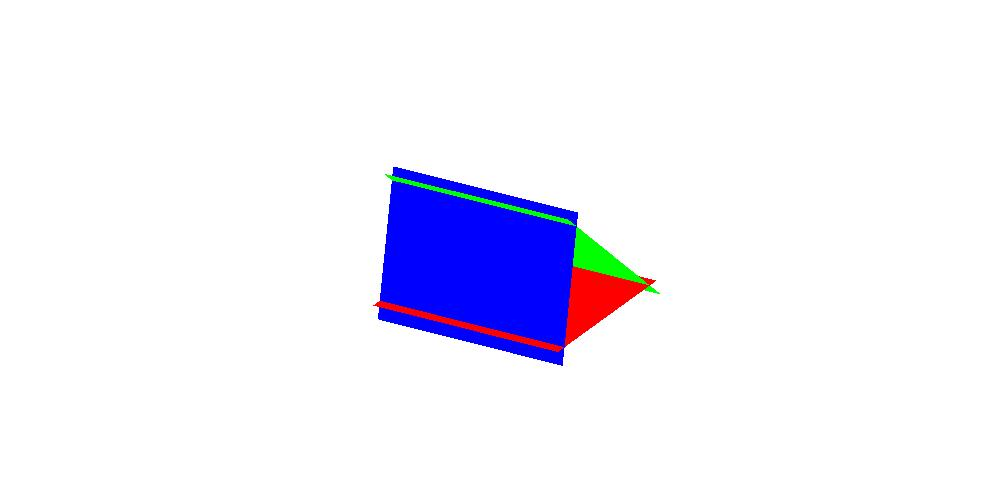
\includegraphics[scale=0.5,clip=true,
      trim=10cm 4.5cm 10cm 5.5cm]{images/toblerone}
 \]

\end{example}

\begin{example}\label{eg-lineq-ii}
 We will solve the equations
 \begin{align*}
  a + b + c + d &= 4 \\
  a + b - c - d &= 0 \\
  a - b + c - d &= 0 \\
  a - b - c + d &= 0.
 \end{align*}
 The corresponding augmented matrix can be row-reduced as follows:
 \[
  \left[\begin{array}{cccc|c}
    1 &  1 &  1 &  1 & 4 \\
    1 &  1 & -1 & -1 & 0 \\
    1 & -1 &  1 & -1 & 0 \\
    1 & -1 & -1 &  1 & 0
  \end{array}\right]
  \xra{1}
  \left[\begin{array}{cccc|c}
    1 &  1 &  1 &  1 &  4 \\
    0 &  0 & -2 & -2 & -4 \\
    1 & -1 &  1 & -1 & 0 \\
    0 &  0 & -2 &  2 & 0
  \end{array}\right]
  \xra{2}
  \left[\begin{array}{cccc|c}
    1 &  1 &  1 &  1 &  4 \\
    0 &  0 &  1 &  1 &  2 \\
    1 & -1 &  1 & -1 & 0 \\
    0 &  0 &  1 & -1 & 0
  \end{array}\right]
  \xra{3}
 \] \[
  \left[\begin{array}{cccc|c}
    1 &  1 &  0 &  0 & 2 \\
    0 &  0 &  1 &  1 & 2 \\
    1 & -1 &  0 &  0 & 0 \\
    0 &  0 &  1 & -1 & 0
  \end{array}\right]
  \xra{4}
  \left[\begin{array}{cccc|c}
    1 &  1 &  0 &  0 & 2 \\
    0 &  0 &  1 &  1 & 2 \\
    0 & -2 &  0 &  0 & -2 \\
    0 &  0 &  0 & -2 & -2
  \end{array}\right]
  \xra{5}
  \left[\begin{array}{cccc|c}
    1 &  1 &  0 &  0 & 2 \\
    0 &  0 &  1 &  1 & 2 \\
    0 &  1 &  0 &  0 & 1 \\
    0 &  0 &  0 &  1 & 1
  \end{array}\right]
  \xra{6}
 \] \[
  \left[\begin{array}{cccc|c}
    1 &  0 &  0 &  0 & 1 \\
    0 &  0 &  1 &  0 & 1 \\
    0 &  1 &  0 &  0 & 1 \\
    0 &  0 &  0 &  1 & 1
  \end{array}\right]
  \xra{7}
  \left[\begin{array}{cccc|c}
    1 &  0 &  0 &  0 & 1 \\
    0 &  1 &  0 &  0 & 1 \\
    0 &  0 &  1 &  0 & 1 \\
    0 &  0 &  0 &  1 & 1
  \end{array}\right]
 \]
 Here, rather than slavishly following Method~\ref{meth-RREF}, we have
 applied row operations in a more creative order to make the structure
 of the equations clearer.  The stages are as follows:
 \begin{itemize}
  \item[1] We subtract the first row from the second, and the third
   from the fourth.
  \item[2] We multiply the second and fourth rows by $-1/2$.
  \item[3] We subtract the second row from the first, and the fourth
   from the third.
  \item[4] We subtract the first row from the third, and the second
   from the fourth.
  \item[5] We multiply the third and fourth rows by $-1/2$.
  \item[6] We subtract the third row from the first, and the fourth
   from the second.
  \item[7] We exchange the second and third rows.
 \end{itemize}
 The final matrix corresponds to the equations $a=1$, $b=1$, $c=1$ and
 $d=1$, which give the unique solution to the original system of
 equations.
\end{example}

\begin{remark}
 Often we want to solve a \dfn{homogeneous} equation $Ax=0$, where
 the right hand side is zero.  This means that the relevant augmented
 matrix is $[A|0]$.  Row operations will not change the fact that the last
 column is zero, so the RREF of $[A|0]$ will just be $[A'|0]$, where
 $A'$ is the RREF of $A$.  In this context we can save writing by
 leaving out the extra column and just working with $A$.
\end{remark}
\begin{example}\label{eg-homogeneous}
 Consider the homogeneous system
 \begin{align*}
  a+b+c+d+e+f &= 0 \\
  2a+2b+2c+2d-e-f &= 0 \\
  3a+3b-c-d-e-f &= 0
 \end{align*}
 The corresponding unaugmented matrix can be row-reduced as follows:
 \[
  \bbm
    1 &  1 &  1 &  1 &  1 &  1 \\
    2 &  2 &  2 &  2 & -1 & -1 \\
    3 &  3 & -1 & -1 & -1 & -1
  \ebm \to \bbm
    1 &  1 &  0 &  0 &  0 &  0 \\
    0 &  0 &  1 &  1 &  0 &  0 \\
    0 &  0 &  0 &  0 &  1 &  1 
  \ebm
 \]
 (details are left to the reader).  The final matrix corresponds to
 the homogeneous system
 \[ a+b = 0 \hspace{5em} c+d=0 \hspace{5em} e+f=0. \]
 There are pivots in columns $1$, $3$ and $5$, meaning that $a$, $c$
 and $e$ are dependent variables, and $b$, $d$ and $f$ are
 independent.  After moving the independent variables to the right
 hand side, the solution becomes $a=-b$, $c=-d$ and $e=-f$.  If we
 prefer we can introduce new variables $\lm$, $\mu$ and $\nu$, and say
 that the general solution is
 \begin{align*}
  a &= -\lm & c &= -\mu & e &= -\nu \\
  b &=  \lm & d &=  \mu & f &=  \nu
 \end{align*}
 for arbitrary values of $\lm$, $\mu$ and $\nu$.
\end{example}

\section{Linear combinations}
\label{sec-lin-comb}

\begin{definition}\label{defn-lincomb}
 Let $v_1,\dotsc,v_k$ and $w$ be vectors in $\R^n$.  We say that $w$
 is a \dfn{linear combination} of $v_1,\dotsc,v_k$ if there exist
 scalars $\lm_1,\dots,\lm_k$ such that
 \[ w = \lm_1v_1 + \dotsb + \lm_kv_k. \]
\end{definition}

\begin{example}\label{eg-lincomb-i}
 Consider the following vectors in $\R^4$:
 \[ v_1 = \bbm 1 \\ -1 \\ 0 \\ 0 \ebm \hspace{3em}
    v_2 = \bbm 0 \\ 1 \\ -1 \\ 0 \ebm \hspace{3em}
    v_3 = \bbm 0 \\ 0 \\ 1 \\ -1 \ebm \hspace{3em}
    w   = \bbm 1 \\ 10 \\ 100 \\ -111 \ebm
 \]
 If we take $\lm_1=1$ and $\lm_2=11$ and $\lm_3=111$ we get
 \[ \lm_1 v_1 + \lm_2 v_2 + \lm_3 v_3 =
     \bbm 1 \\ -1 \\ 0 \\ 0 \ebm +
     \bbm 0 \\ 11 \\ -11 \\ 0 \ebm +
     \bbm 0 \\ 0 \\ 111 \\ -111 \ebm =
     \bbm 1 \\ 10 \\ 100 \\ -111 \ebm = w,
 \]
 which shows that $w$ is a linear combination of $v_1$, $v_2$ and
 $v_3$.
\end{example}

\begin{example}\label{eg-lincomb-ii}
 Consider the following vectors in $\R^4$:
 \[ v_1 = \bbm 0 \\ 1 \\  2 \\  3 \ebm \hspace{3em}
    v_2 = \bbm 0 \\ 1 \\  4 \\  9 \ebm \hspace{3em}
    v_3 = \bbm 0 \\ 1 \\  8 \\ 27 \ebm \hspace{3em}
    v_4 = \bbm 0 \\ 1 \\ 16 \\ 81 \ebm \hspace{3em}
    w = \bbm 1 \\ 1 \\ 1 \\ 1 \ebm.
 \]
 Any linear combination of $v_1,\dotsc,v_4$ has the form
 \[ \lm_1v_1 + \lm_2v_2 + \lm_3v_3 + \lm_4v_4 =
     \bbm 0 \\ \lm_1+\lm_2+\lm_3+\lm_4 \\
          2\lm_1+4\lm_2+8\lm_3+16\lm_4 \\
          3\lm_1+9\lm_2+27\lm_3+81\lm_4 \ebm.
 \]
 In particular, the first component of any such linear combination is
 zero.  (You should be able to see this without needing to write out
 the whole formula.)  As the first component of $w$ is not zero, we
 see that $w$ is \emph{not} a linear combination of $v_1,\dotsc,v_4$.
\end{example}

\begin{example}\label{eg-lincomb-iii}
 Consider the following vectors in $\R^3$:
 \[ v_1 = \bbm 1 \\ 1 \\ 1 \ebm \hspace{3em}
    v_2 = \bbm 1 \\ 2 \\ 1 \ebm \hspace{3em}
    v_3 = \bbm 1 \\ 3 \\ 1 \ebm \hspace{3em}
    v_4 = \bbm 1 \\ 4 \\ 1 \ebm \hspace{3em}
    v_5 = \bbm 1 \\ 5 \\ 1 \ebm \hspace{3em}
    w   = \bbm -1 \\ 0 \\ 1 \ebm.
 \]
 Any linear combination of $v_1,\dotsc,v_5$ has the form
 \[ \lm_1v_1 + \dotsb + \lm_5v_5 =
     \bbm \lm_1+\lm_2+\lm_3+\lm_4+\lm_5 \\
          \lm_1+2\lm_2+3\lm_3+4\lm_4+5\lm_5 \\
          \lm_1+\lm_2+\lm_3+\lm_4+\lm_5 \ebm.
 \]
 In particular, the first and last components of any such linear
 combination are the same.  Again, you should be able to see this
 without writing the full formula.  As the first and last components
 of $w$ are different, we see that $w$ is not a linear combination of
 $v_1,\dotsc,v_5$.
\end{example}
\begin{example}\label{eg-lincomb-iv}
 Let $v_1$, $v_2$ and $w$ be vectors in $\R^3$ (so we can think about
 them geometrically).  For simplicity, assume that all three vectors
 are nonzero, and that $v_1$ and $v_2$ do not point in the same
 direction, nor do they point in opposite directions.  This will mean
 that there is a unique plane $P$ that passes through $v_1$, $v_2$ and
 the origin.  It is not hard to see that $P$ is just the set of all
 possible linear combinations of $v_1$ and $v_2$.  Thus, our vector
 $w$ is a linear combination of $v_1$ and $v_2$ if and only if $w$
 lies in the plane $P$.
 \[ 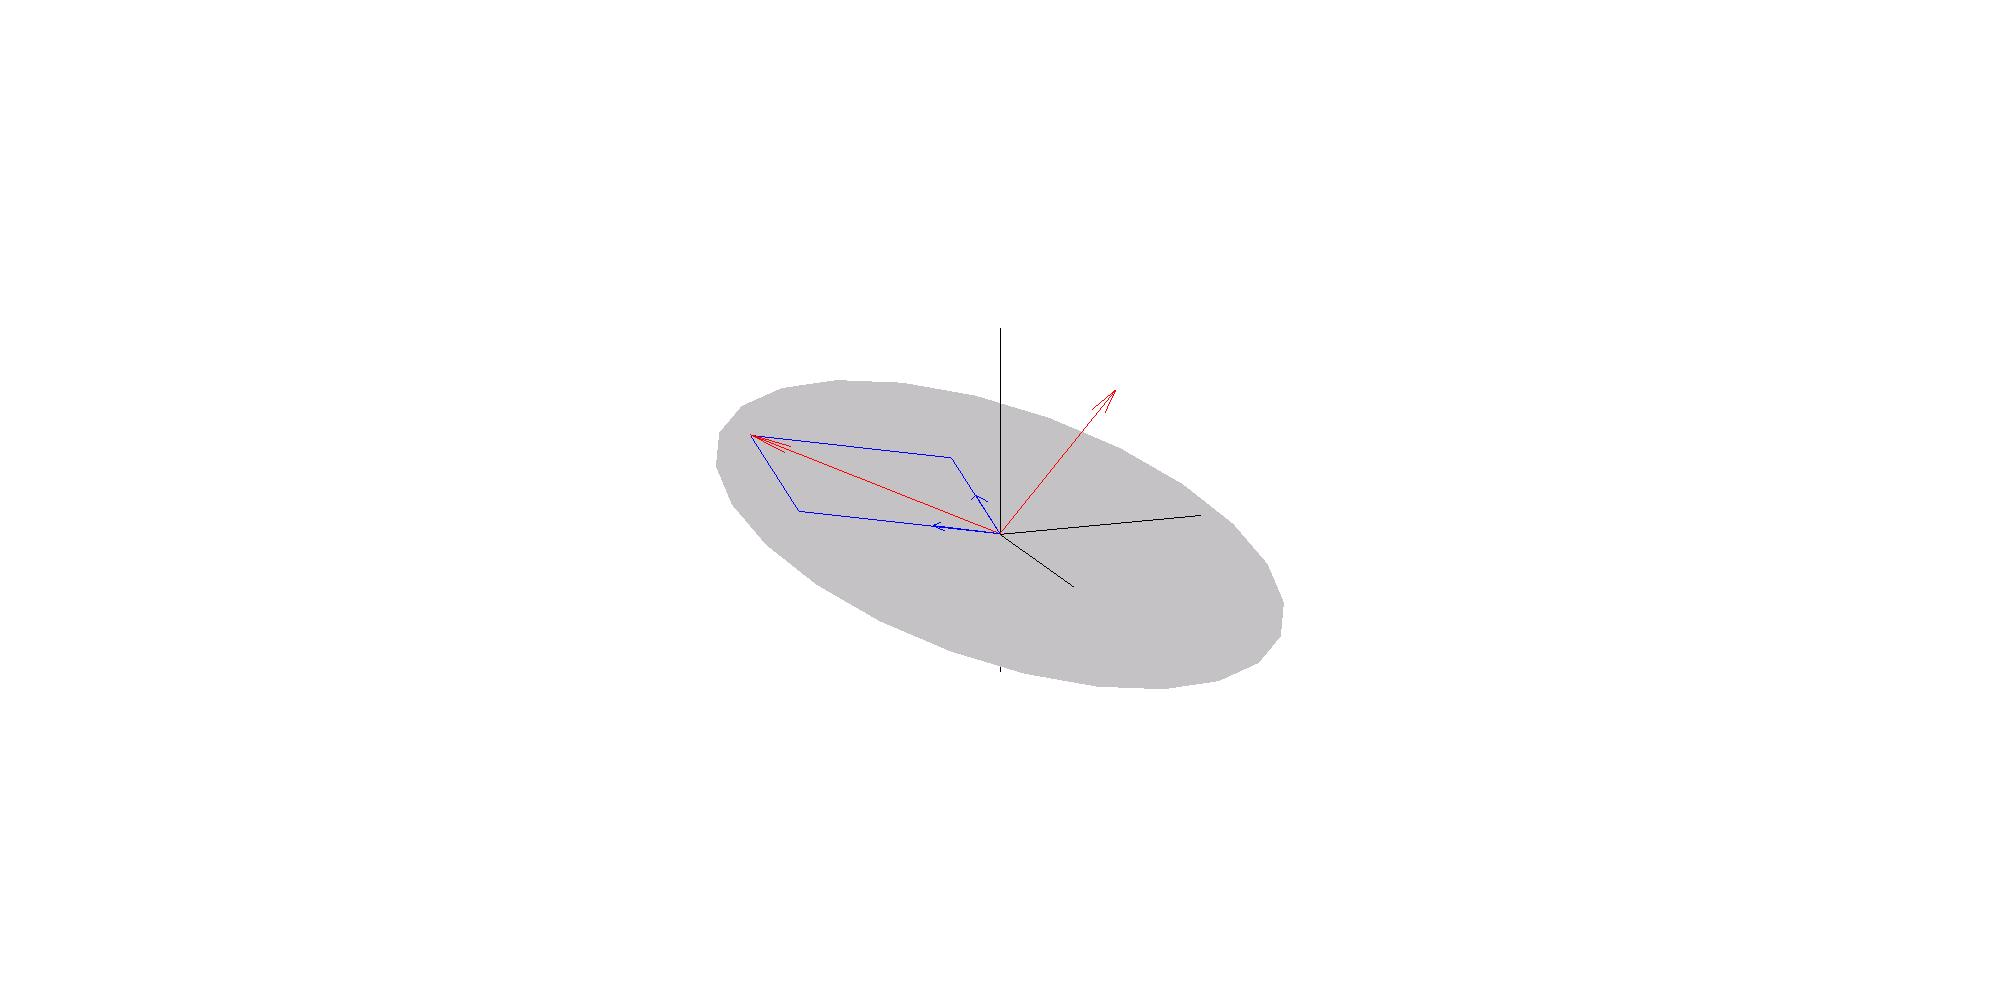
\includegraphics[scale=0.4,clip=true,
      trim=20cm 9cm 20cm 11cm]{images/plane_span}
 \]
\end{example}

We now want to explain a more systematic way to check whether a given
vector is a linear combination of some given list of vectors.
Note that for any $k$-vector
$\lm=\bbm\lm_1 & \dotsb & \lm_k\ebm^T$ we have
\[ A\lm =
    \left[\begin{array}{c|c|c}
     v_1 & \cdots & v_k
    \end{array}\right]
    \bbm \lm_1 \\ \vdots \\ \lm_k \ebm =
    \lm_1 v_1 + \dotsb + \lm_k v_k,
\]
which is the general form for a linear combination of
$v_1,\dotsc,v_k$.  This makes it clear that $w$ is a linear
combination of $v_1,\dotsc,v_k$ if and only if there is a vector $\lm$
which solves the matrix equation $A\lm=w$.  Using
Theorem~\ref{thm-row-ops} we see that the equation $A\lm=w$ has the
same solutions as the equation $A'\lm=w'$, which can be solved easily
by Method~\ref{meth-RREF-solve}.  We thus arrive at the following
method: 

\begin{method}\label{meth-find-lincomb}
 \index{linear combination}
 Suppose we have vectors $v_1,\dotsc,v_k\in\R^n$ and another vector
 $w\in\R^n$, and we want to express $w$ as a linear combination of the
 $v_i$ (or show that this is not possible).
 \begin{itemize}
  \item[(a)] We first let $A$ be the matrix whose columns are the
   vectors $v_i$:
   \[ A = \left[\begin{array}{c|c|c}
       v_1 & \cdots & v_k
      \end{array}\right] \in M_{n\tm k}(\R).
   \]
  \item[(b)] We then append $w$ as an additional column to get an
   augmented matrix
   \[ B  = \left[\begin{array}{c|c|c|c}
       v_1 & \cdots & v_k & w
      \end{array}\right]
       = \left[\begin{array}{c|c} A & w\end{array}\right].
   \]
   This corresponds to the matrix equation $A\lm=w$.
  \item[(c)] Row-reduce $B$ by Method~\ref{meth-RREF} to get a matrix
   $B'=[A'|w']$ in RREF.
  \item[(d)] If $B'$ has a pivot in the last column, then $w$ is not a
   linear combination of the vectors $v_1,\dotsc,v_k$.
  \item[(e)] If $B'$ has no pivot in the last column, then we can use
   Method~\ref{meth-RREF-solve} to find a vector
   $\lm=\bbm\lm_1 & \cdots & \lm_k\ebm^T$ satisfying $A'\lm=w'$.  We
   then have $A\lm=w$ and $\lm_1v_1+\dotsb+\lm_kv_k=w$, showing that
   $w$ is a linear combination of $v_1,\dotsc,v_k$.
 \end{itemize}
\end{method}

\begin{example}\label{eg-find-lincomb-i}
 Consider the vectors
 \[ v_1 = \bbm 11 \\ 11 \\ 1 \\ 1 \ebm \hspace{3em}
    v_2 = \bbm 1 \\ 11 \\ 11 \\ 1 \ebm \hspace{3em}
    v_3 = \bbm 1 \\ 1 \\ 11 \\ 11 \ebm \hspace{3em}
    w   = \bbm 121 \\ 221 \\ 1211 \\ 1111 \ebm.
 \]
 We ask whether $w$ can be expressed as a linear combination
 $w=\lm_1v_1+\lm_2v_2+\lm_3v_3$, and if so, what are the relevant
 values $\lm_1$, $\lm_2$ and $\lm_3$?  Following
 Method~\ref{meth-find-lincomb}, we write down the augmented
 matrix $[v_1|v_2|v_3|w]$ and row-reduce it:
 \[
  \left[\begin{array}{ccc|c}
   11 &  1 &  1 & 121 \\
   11 & 11 &  1 & 221 \\
    1 & 11 & 11 & 1211 \\
    1 &  1 & 11 & 1111
  \end{array}\right]
  \xra{1}
  \left[\begin{array}{ccc|c}
    1 &  1 & 11 & 1111 \\
   11 &  1 &  1 & 121 \\
   11 & 11 &  1 & 221 \\
    1 & 11 & 11 & 1211
  \end{array}\right]
  \xra{2}
  \left[\begin{array}{ccc|c}
    1 &   1 &   11 & 1111 \\
    0 & -10 & -120 & -12100 \\
    0 &   0 & -120 & -12000 \\
    0 &  10 &    0 & 100
  \end{array}\right]
  \xra{3}
 \] \[
  \left[\begin{array}{ccc|c}
    1 &   1 &   11 & 1111 \\
    0 &   1 &   12 & 1210 \\
    0 &   0 &    1 & 100 \\
    0 &   1 &    0 & 10
  \end{array}\right]
  \xra{4}
  \left[\begin{array}{ccc|c}
    1 &   1 &    0 & 11 \\
    0 &   1 &    0 & 10 \\
    0 &   0 &    1 & 100 \\
    0 &   1 &    0 & 10
  \end{array}\right]
  \xra{5}
  \left[\begin{array}{ccc|c}
    1 &   0 &    0 & 1 \\
    0 &   1 &    0 & 10 \\
    0 &   0 &    1 & 100 \\
    0 &   0 &    0 & 0
  \end{array}\right]
 \]
 (1: move the bottom row to the top; 2: subtract multiples of row 1
 from the other rows; 3: divide rows 2,3 and 4 by $-10$, $-120$ and
 $10$; 4: subtract multiples of row 3 from the other rows; 5: subtract
 multiples of row 2 from the other rows.)

 The final matrix corresponds to the system of equations
 \[ \lm_1 = 1 \hspace{3em}
    \lm_2 = 10 \hspace{3em}
    \lm_3 = 100 \hspace{3em}
     0 = 0
 \]
 so we conclude that
 \[ w = v_1 + 10 v_2 + 100 v_3. \]
 In particular, $w$ can be expressed as a linear combination of $v_1$,
 $v_2$ and $v_3$.  We can check the above equation directly:
 \[ v_1 + 10 v_2 + 100 v_3 =
      \bbm  11 \\  11 \\    1 \\    1 \ebm +
      \bbm  10 \\ 110 \\  110 \\   10 \ebm +
      \bbm 100 \\ 100 \\ 1100 \\ 1100 \ebm
    = \bbm 121 \\ 221 \\ 1211 \\ 1111 \ebm = w.
 \]
\end{example}

\begin{example}\label{eg-find-lincomb-ii}
 Consider the vectors
 \[ a_1 = \bbm 2 \\ -1 \\  0 \ebm \hspace{3em}
    a_2 = \bbm 3 \\  0 \\ -1 \ebm \hspace{3em}
    a_3 = \bbm 0 \\  3 \\ -2 \ebm \hspace{3em}
    b = \bbm 1 \\ 2 \\ 3 \ebm
 \]
 To test whether $b$ is a linear combination of $a_1$, $a_2$ and
 $a_3$, we write down the relevant augmented matrix and row-reduce it:
 \[
  \left[\begin{array}{ccc|c}
    2 &  3 &  0 & 1 \\
   -1 &  0 &  3 & 2 \\
    0 & -1 & -2 & 3
  \end{array}\right]
  \xra{1}
  \left[\begin{array}{ccc|c}
    1 &  0 & -3 & -2 \\
    0 &  1 &  2 & -3 \\
    2 &  3 &  0 &  1
  \end{array}\right]
  \xra{2}
  \left[\begin{array}{ccc|c}
    1 &  0 & -3 & -2 \\
    0 &  1 &  2 & -3 \\
    0 &  3 &  6 &  5
  \end{array}\right]
  \xra{3}
 \] \[
  \left[\begin{array}{ccc|c}
    1 &  0 & -3 & -2 \\
    0 &  1 &  2 & -3 \\
    0 &  0 &  0 & 14
  \end{array}\right]
  \xra{4}
  \left[\begin{array}{ccc|c}
    1 &  0 & -3 & -2 \\
    0 &  1 &  2 & -3 \\
    0 &  0 &  0 &  1
  \end{array}\right]
  \xra{5}
  \left[\begin{array}{ccc|c}
    1 &  0 & -3 &  0 \\
    0 &  1 &  2 &  0 \\
    0 &  0 &  0 &  1
  \end{array}\right]
 \]
 (Stage 1: move the top row to the bottom, and multiply the other two rows
 by $-1$; Stage 2: subtract $2$ times row 1 from row 3; Stage 3:
 subtract $3$ times row 2 from row 3; Stage 4: divide row 3 by $14$;
 Stage 5: subtract multiples of row 3 from rows 1 and 2.)

 The last matrix has a pivot in the rightmost column, corresponding to
 the equation $0=1$.  This means that the equation
 $\lm_1a_1+\lm_2a_2+\lm_3a_3=b$ cannot be solved for $\lm_1$, $\lm_2$
 and $\lm_3$, or in other words that $b$ is not a linear combination
 of $a_1$, $a_2$ and $a_3$.

 We can also see this in a more direct but less systematic way, as
 follows.  It is easy to check that $b.a_1=b.a_2=b.a_3=0$, which means
 that $b.(\lm_1a_1+\lm_2a_2+\lm_3a_3)=0$ for all possible choices of
 $\lm_1$, $\lm_2$ and $\lm_3$.  However, $b.b=14>0$, so $b$ cannot be
 equal to $\lm_1a_1+\lm_2a_2+\lm_3a_3$.
\end{example}

\section{Linear independence}

\begin{definition}\label{defn-dependent}
 Let $\CV=v_1,\dotsc,v_k$ be a list of vectors in $\R^n$.  A
 \dfn{linear relation} between the vectors $v_i$ is a relation of the
 form $\lm_1v_1+\dotsb+\lm_kv_k=0$, where $\lm_1,\dotsc,\lm_k$ are
 scalars.  In other words, it is a way of expressing $0$ as a linear
 combination of $\CV$.

 For any list we have the trivial linear relation
 $0v_1+0v_2+\dotsb+0v_k=0$.  There may or may not be any nontrivial
 linear relations.

 If the list $\CV$ has a nontrivial linear relation, we say that it is
 a \dfn{linearly dependent} list.  If the only linear relation on
 $\CV$ is the trivial one, we instead say that $\CV$ is \dfn{linearly
  independent}.  We will often omit the word ``linearly'' for the sake
 of brevity.
\end{definition}

\begin{example}\label{eg-dep-i}
 Consider the list $\CV$ given by
 \[ v_1 = \bbm 1 \\ 1 \\ 0 \\ 0 \ebm \hspace{3em}
    v_2 = \bbm 0 \\ 0 \\ 1 \\ 1 \ebm \hspace{3em}
    v_3 = \bbm 1 \\ 0 \\ 0 \\ 1 \ebm \hspace{3em}
    v_4 = \bbm 0 \\ 1 \\ 1 \\ 0 \ebm.
 \]
 There is a nontrivial linear relation $v_1+v_2-v_3-v_4=0$, so the
 list $\CV$ is dependent.
\end{example}
\begin{example}\label{eg-dep-ii}
 Consider the list $\CA$ given by
 \[ a_1 = \bbm  1 \\  2 \ebm \hspace{3em}
    a_2 = \bbm 12 \\  1 \ebm \hspace{3em}
    a_3 = \bbm -1 \\ -1 \ebm \hspace{3em}
    a_4 = \bbm  3 \\  1 \ebm.
 \]
 Just by writing it out, you can check that
 \[ 3a_1 + a_2 + 3a_3 -4a_4 = 0. \]
 \begin{center}
  \begin{tikzpicture}[scale=0.3]
   \fill( 0,0) circle(0.1);
   \fill( 3,6) circle(0.1);
   \fill(15,7) circle(0.1);
   \fill(12,4) circle(0.1);
   \draw[->, shorten >= 1pt] (0,0) -- (3,6);
   \draw[->, shorten >= 1pt] (3,6) -- (15,7);
   \draw[->, shorten >= 1pt] (15,7) -- (12,4);
   \draw[->, shorten >= 1pt] (12,4) -- (0,0);
   \draw ( 1.5,3.0) node[anchor=south east]{$\ss 3a_1$};
   \draw ( 9.0,6.5) node[anchor=south]{$\ss a_2$};
   \draw (13.5,5.5) node[anchor=north west]{$\ss 3a_3$};
   \draw ( 6.0,2.0) node[anchor=north]{$\ss -4a_4$};
  \end{tikzpicture}
 \end{center}
 This is a nontrivial linear relation on the list $\CA$, so $\CA$ is
 dependent.
\end{example}
\begin{example}\label{eg-indep-i}
 Consider the list $\CU$ given by
 \[ u_1 = \bbm 1 \\ 1 \\ 0 \\ 0 \ebm \hspace{3em}
    u_2 = \bbm 0 \\ 1 \\ 1 \\ 0 \ebm \hspace{3em}
    u_3 = \bbm 0 \\ 0 \\ 1 \\ 1 \ebm.
 \]
 We claim that this is independent.  To see this, consider a linear
 relation $\lm_1u_1+\lm_2u_2+\lm_3u_3=0$.  Writing this out, we get
 \[ \bbm \lm_1 \\ \lm_1+\lm_2 \\ \lm_2+\lm_3 \\ \lm_3 \ebm =
    \bbm 0 \\ 0 \\ 0 \\ 0 \ebm.
 \]
 By looking at the first and last rows we see that $\lm_1=\lm_3=0$.
 By looking at the second row we get $\lm_2=-\lm_1=0$ as well so our
 relation is the trivial relation.  As the only linear relation is the
 trivial one, we see that $\CU$ is independent.
\end{example}

\begin{lemma}\label{lem-multiples}
 Let $v$ and $w$ be vectors in $\R^n$, and suppose that $v\neq 0$ and
 that the list $(v,w)$ is linearly dependent.  Then there is a number
 $\al$ such that $w=\al v$.
\end{lemma}
\begin{proof}
 Because the list is dependent, there is a linear relation
 $\lm v+\mu w=0$ where $\lm$ and $\mu$ are not both zero.  There are
 apparently three possibilities: (a) $\lm\neq 0$ and $\mu\neq 0$; (b)
 $\lm=0$ and $\mu\neq 0$; (c) $\lm\neq 0$ and $\mu=0$.  However,
 case~(c) is not really possible.  Indeed, in case~(c) the equation
 $\lm v+\mu w=0$ would reduce to $\lm v=0$, and we could multiply by
 $\lm^{-1}$ to get $v=0$; but $v\neq 0$ by assumption.  In case~(a)
 or~(b) we can take $\al=-\lm/\mu$ and we have $w=\al v$.
\end{proof}

There is a systematic method using row-reduction for checking linear
(in)dependence, as we will explain shortly.  We first need a
preparatory observation.

\begin{definition}\label{defn-wide}
 Let $B$ be a $p\tm q$ matrix.  We say that $B$ is \dfn{wide} if
 $p<q$, or \dfn{square} if $p=q$ or \dfn{tall} if $p>q$.
 \[ \begin{array}{ccccc}
     \bbm 1 & 2 & 3 \\ 4 & 5 & 6 \ebm & &
     \bbm 1 & 2 & 1 \\ 2 & 3 & 2 \\ 1 & 2 & 1 \ebm & &
     \bbm 1 & 1 \\ 0 & 0 \\ 1 & 1 \ebm \\
     \text{ wide } & & \text{ square } & & \text{ tall }
    \end{array}
 \]
\end{definition}
\begin{lemma}\label{lem-pivots-everywhere}
 \index{pivot}
 Let $B$ be a $p\tm q$ matrix in RREF.
 \begin{itemize}
  \item[(a)] If $B$ is wide then it is impossible for every column to
   contain a pivot.
  \item[(b)] If $B$ is square then the only way for every column to
   contain a pivot is if $B=I_q$.
  \item[(c)] If $B$ is tall  then the only way for every column to
   contain a pivot is if $B$ consists of $I_q$ with $(p-q)$ rows of
   zeros added at the bottom (so
   $B=\left[\begin{array}{c} I_q \\ \hline 0_{(p-q)\tm q}
      \end{array}\right]$).
 \end{itemize}
\end{lemma}

For example, the only $5\tm 3$ RREF matrix with a pivot in every
column is this one:
\[ \left[\begin{array}{c}
      I_3 \\ \hline 0_{2\tm 3} 
   \end{array}\right] =
   \left[\begin{array}{ccc}
    1 & 0 & 0 \\
    0 & 1 & 0 \\
    0 & 0 & 1 \\ \hline
    0 & 0 & 0 \\
    0 & 0 & 0
   \end{array}\right]
\]

\begin{proof}
 There is at most one pivot in every row, making at most $p$ pivots
 altogether.  If $B$ is wide then we have $q$ columns with $q>p$, so
 there are not enough pivots to have one in every column.  This
 proves~(a).

 Now suppose instead that $B$ does have a pivot in every column, so
 there are $q$ pivots and we must have $p\geq q$.  As $B$ is in RREF
 we know that all entries above or below a pivot are zero.  As there
 is a pivot in every column it follows that the pivots are the only
 nonzero entries in $B$.  Every nonzero row contains precisely one
 pivot, so there must be $q$ nonzero rows.  The remaining $(p-q)$ rows
 are all zero, and they must occur at the bottom of $B$ (because $B$
 is in RREF).  Now the top $q\tm q$ block contains $q$ pivots which
 move to the right as we go down the matrix.  It is easy to see that
 the only possibility for the top block is $I_q$, which proves~(b)
 and~(c).
\end{proof}

\begin{method}\label{meth-check-dependence}
 \index{linearly dependent}\index{linearly independent}\index{pivot}
 Let $\CV=v_1,\dotsc,v_m$ be a list of vectors in $\R^n$.  We can
 check whether this list is dependent as follows.
 \begin{itemize}
  \item[(a)] Form the $n\tm m$ matrix
   \[ A = \left[\begin{array}{c|c|c}
              && \\
              v_1 & \dotsc & v_m \\
              &&
            \end{array}\right]
   \]
   whose columns are the vectors $v_i$.
  \item[(b)] Row reduce $A$ to get another $n\tm m$ matrix $B$ in
   RREF.
  \item[(c)] If every column of $B$ contains a pivot (so $B$ has the
   form discussed in Lemma~\ref{lem-pivots-everywhere}) then $\CV$ is
   independent.
  \item[(d)] If some column of $B$ has no pivot, then the list $\CV$
   is dependent.  Moreover, we can find the coefficients $\lm_i$ in a
   nontrivial linear relation by solving the vector equation $B\lm=0$
   (which is easy because $B$ is in RREF).
 \end{itemize}
\end{method}
\begin{remark}\label{rem-dependence-shortcut}
 \index{wide}\index{numerical criteria}
 If $m>n$ then $\CV$ is automatically dependent and we do not need to
 go through the method.  (For example, any list of $5$ vectors in
 $\R^3$ is automatically dependent, any list of $10$ vectors in $\R^9$
 is automatically dependent, and so on.)  Indeed, in this case the
 matrices $A$ and $B$ are wide, so it is impossible for $B$ to have a
 pivot in every column.  However, this line of argument only tells us
 that there \textbf{exists} a nontrivial relation
 $\lm_1v_1+\dotsb+\lm_mv_m=0$, it does not tell us the coefficients
 $\lm_i$.  If we want to find the $\lm_i$ then we do need to go
 through the whole method as explained above.
\end{remark}

We will give some examples of using the above method, and then explain
why the method is correct.

\begin{example}\label{eg-dep-i-matrix}
 In example~\ref{eg-dep-i} we considered the list
 \[ v_1 = \bbm 1 \\ 1 \\ 0 \\ 0 \ebm \hspace{3em}
    v_2 = \bbm 0 \\ 0 \\ 1 \\ 1 \ebm \hspace{3em}
    v_3 = \bbm 1 \\ 0 \\ 0 \\ 1 \ebm \hspace{3em}
    v_4 = \bbm 0 \\ 1 \\ 1 \\ 0 \ebm.
 \]
 We can write down the corresponding matrix and row-reduce it as
 follows:
 \[
  \bbm 1 & 0 & 1 & 0 \\
       1 & 0 & 0 & 1 \\
       0 & 1 & 0 & 1 \\
       0 & 1 & 1 & 0
  \ebm \xra{1}
  \bbm 1 & 0 & 1 & 0 \\
       0 & 0 &-1 & 1 \\
       0 & 1 & 0 & 1 \\
       0 & 0 & 1 &-1
  \ebm \xra{2}
  \bbm 1 & 0 & 1 & 0 \\
       0 & 1 & 0 & 1 \\
       0 & 0 & 1 &-1 \\
       0 & 0 &-1 & 1
  \ebm \xra{3}
  \bbm 1 & 0 & 0 & 1 \\
       0 & 1 & 0 & 1 \\
       0 & 0 & 1 &-1 \\
       0 & 0 & 0 & 0
  \ebm
 \]
 The end result has no pivot in the last column, so the original list is
 dependent.  To find a specific linear relation, we solve the equation
 \[   \bbm 1 & 0 & 0 & 1 \\
           0 & 1 & 0 & 1 \\
           0 & 0 & 1 &-1 \\
           0 & 0 & 0 & 0
      \ebm
      \bbm \lm_1 \\ \lm_2 \\ \lm_3 \\ \lm_4 \ebm =
      \bbm 0 \\ 0 \\ 0 \\ 0 \ebm
 \]
 to get $\lm_1=-\lm_4$, $\lm_2=-\lm_4$ and $\lm_3=\lm_4$ with $\lm_4$
 arbitrary.  Taking $\lm_4=1$ gives
 $(\lm_1,\lm_2,\lm_3,\lm_4)=(-1,-1,1,1)$, corresponding to the
 relation $-v_1-v_2+v_3+v_4=0$.
\end{example}
\begin{example}\label{eg-dep-ii-matrix}
 In Example~\ref{eg-dep-ii} we considered the list
 \[ a_1 = \bbm  1 \\  2 \ebm \hspace{3em}
    a_2 = \bbm 12 \\  1 \ebm \hspace{3em}
    a_3 = \bbm -1 \\ -1 \ebm \hspace{3em}
    a_4 = \bbm  3 \\  1 \ebm.
 \]
 Here we have $4$ vectors in $\R^2$, so they must be dependent by
 Remark~\ref{rem-dependence-shortcut}.  Thus, there exist nontrivial
 linear relations
 \[ \lm_1a_1 + \lm_2a_2 + \lm_3a_3 + \lm_4a_4 = 0. \]
 To actually find such a relation, we write down the corresponding
 matrix and row-reduce it as follows:
 \[
  \bbm
   1 & 12 & -1 & 3 \\
   2 & 1  & -1 & 1
  \ebm
  \xra{}
  \bbm
   1 &  12 & -1 & 3 \\
   0 & -23 &  1 & -5
  \ebm
  \xra{}
  \bbm
   1 &  12 & -1 & 3 \\
   0 &  1 & -1/23 & 5/23
  \ebm
  \xra{}
  \bbm
   1 &  0 & -11/23 & 9/23 \\
   0 &  1 & -1/23 & 5/23
  \ebm
 \]
 We now need to solve the matrix equation
 \[ \bbm
     1 &  0 & -11/23 & 9/23 \\
     0 &  1 & -1/23 & 5/23
    \ebm
    \bbm \lm_1 \\ \lm_2 \\ \lm_3 \\ \lm_4 \ebm =
    \bbm 0 \\ 0 \ebm
 \]
 As this is in RREF, we can just read off the solution:
 $\lm_1=\frac{11}{23}\lm_3-\frac{9}{23}\lm_4$ and
 $\lm_2=\frac{1}{23}\lm_3-\frac{5}{23}\lm_4$
 with $\lm_3$ and $\lm_4$ arbitrary.  If we choose $\lm_3=23$ and
 $\lm_4=0$ we get $(\lm_1,\lm_2,\lm_3,\lm_4)=(11,1,23,0)$ so we have a
 relation
 \[ 11 a_1 + a_2 + 23 a_3 + 0 a_4 = 0. \]
 (You should check directly that this is correct.)  Alternatively, we
 can choose $\lm_3=3$ and $\lm_4=-4$.  Using the equations
 $\lm_1=\frac{11}{23}\lm_3-\frac{9}{23}\lm_4$ and
 $\lm_2=\frac{1}{23}\lm_3-\frac{5}{23}\lm_4$ we get $\lm_1=3$ and
 $\lm_2=1$ giving a different relation
 \[ 3a_1 + a_2 + 3a_3 - 4a_4 = 0. \]
 This is the relation that we observed in Example~\ref{eg-dep-ii}.
\end{example}
\begin{example}\label{eg-indep-i-matrix}
 In Example~\ref{eg-indep-i} we considered the list $\CU$ given by
 \[ u_1 = \bbm 1 \\ 1 \\ 0 \\ 0 \ebm \hspace{3em}
    u_2 = \bbm 0 \\ 1 \\ 1 \\ 0 \ebm \hspace{3em}
    u_3 = \bbm 0 \\ 0 \\ 1 \\ 1 \ebm.
 \]
 We can write down the corresponding matrix and row-reduce it as
 follows:
 \[
  \bbm
   1 & 0 & 0 \\
   1 & 1 & 0 \\
   0 & 1 & 1 \\
   0 & 0 & 1
  \ebm
  \to
  \bbm
   1 & 0 & 0 \\
   0 & 1 & 0 \\
   0 & 1 & 1 \\
   0 & 0 & 1
  \ebm
  \to
  \bbm
   1 & 0 & 0 \\
   0 & 1 & 0 \\
   0 & 0 & 1 \\
   0 & 0 & 1
  \ebm
  \to
  \left[\begin{array}{ccc}
   1 & 0 & 0 \\
   0 & 1 & 0 \\
   0 & 0 & 1 \\ \hline
   0 & 0 & 0
  \end{array}\right]
 \]
 The final matrix has a pivot in every column, as in
 Lemma~\ref{lem-pivots-everywhere}.  It follows that the list $\CU$ is
 independent.
\end{example}

\begin{proof}[Proof of correctness of Method~\ref{meth-check-dependence}]
 Put
 \[ A = \left[\begin{array}{c|c|c}
              && \\
              v_1 & \cdots & v_m \\
              &&
        \end{array}\right]
 \]
 as in step~(a) of the method, and let $B$ be the RREF form of $A$.
 Note that for any vector
 $\lm=\bbm \lm_1 & \dotsc & \lm_m\ebm^T\in\R^m$, we have
 \[ A\lm =
     \left[\begin{array}{c|c|c}
              && \\
              v_1 & \cdots & v_m \\
              &&
     \end{array}\right]
     \bbm \lm_1 \\ \vdots \\ \lm_m \ebm =
     \lm_1v_1 + \dotsb + \lm_mv_m.
 \]
 Thus, linear relations on our list are just the same as solutions to
 the homogeneous equation $A\lm=0$.  By Theorem~\ref{thm-row-ops},
 these are the same as solutions to the equation $B\lm=0$, which can
 be found by Method~\ref{meth-RREF-solve}.  If there is a pivot in
 every column then none of the variables $\lm_i$ is independent, so
 the only solution is $\lm_1=\lm_2=\dotsb=\lm_m=0$.  Thus, the only
 linear relation on $\CV$ is the trivial one, which means that the
 list $\CV$ is linearly independent.

 Suppose instead that some column (the $k$'th one, say) does not
 contain a pivot.  Then in Method~\ref{meth-RREF-solve} the variable
 $\lm_k$ will be independent, so we can choose $\lm_k=1$.  This will
 give us a nonzero solution to $B\lm=0$, or equivalently $A\lm=0$,
 corresponding to a nontrivial linear relation on $\CV$.  This shows
 that $\CV$ is linearly dependent.
\end{proof}

\section{Spanning sets}
\label{sec-spanning}

\begin{definition}\label{defn-spanning-list}
 Suppose we have a list $\CV=v_1,\dotsc,v_m$ of vectors in $\R^n$.  We
 say that the list \emph{spans}\index{span} $\R^n$ if \textbf{every} vector in
 $\R^n$ can be expressed as a linear combination of $v_1,\dotsc,v_m$.
\end{definition}
\begin{example}\label{eg-not-span-i}
 Consider the list $\CV=v_1,v_2,v_3,v_4$, where
 \[ v_1 = \bbm 0 \\ 1 \\  2 \\  3 \ebm \hspace{3em}
    v_2 = \bbm 0 \\ 1 \\  4 \\  9 \ebm \hspace{3em}
    v_3 = \bbm 0 \\ 1 \\  8 \\ 27 \ebm \hspace{3em}
    v_4 = \bbm 0 \\ 1 \\ 16 \\ 81 \ebm
 \]
 In Example~\ref{eg-lincomb-ii} we saw that the vector
 $w=\bbm 1 & 1 & 1 & 1\ebm^T$ is not a linear combination of this
 list, so the list $\CV$ does not span $\R^4$.
\end{example}
\begin{example}\label{eg-not-span-ii}
 Consider the list $\CV=v_1,v_2,v_3,v_4,v_5$, where
 \[ v_1 = \bbm 1 \\ 1 \\ 1 \ebm \hspace{3em}
    v_2 = \bbm 1 \\ 2 \\ 1 \ebm \hspace{3em}
    v_3 = \bbm 1 \\ 3 \\ 1 \ebm \hspace{3em}
    v_4 = \bbm 1 \\ 4 \\ 1 \ebm \hspace{3em}
    v_5 = \bbm 1 \\ 5 \\ 1 \ebm.
 \]
 In Example~\ref{eg-lincomb-iii} we saw that the vector
 $w=\bbm -1 & 0 & 1 \ebm^T$ is not a linear combination of this
 list, so the list $\CV$ does not span $\R^3$.
\end{example}
\begin{example}\label{eg-not-span-iii}
 Similarly, Example~\ref{eg-find-lincomb-ii} shows that the list
 \[ \CA = \bbm 2 \\ -1 \\  0 \ebm, \qquad
          \bbm 3 \\  0 \\ -1 \ebm, \qquad
          \bbm 0 \\  3 \\ -2 \ebm
 \]
 does not span $\R^3$.
\end{example}

\begin{example}\label{eg-span-i}
 Consider the list $\CU=u_1,u_2,u_3$, where
 \[ u_1 = \bbm 1 \\ 1 \\ 0 \ebm \hspace{3em}
    u_2 = \bbm 1 \\ 0 \\ 1 \ebm \hspace{3em}
    u_3 = \bbm 0 \\ 1 \\ 1 \ebm.
 \]
 We will show that these span $\R^3$.  Indeed, for any vector
 $v=\bbm x & y & z\ebm^T\in\R^3$ we can put
 \[ \lm_1 = \frac{ x+y-z}{2} \hspace{4em}
    \lm_2 = \frac{ x-y+z}{2} \hspace{4em}
    \lm_3 = \frac{-x+y+z}{2}
 \]
 and we find that
 \begin{align*}
  \lm_1u_1+\lm_2u_2+\lm_3u_3
    &=
   \bbm (x+y-z)/2 \\ (x+y-z)/2 \\ 0 \ebm +
   \bbm (x-y+z)/2 \\ 0 \\ (x-y+z)/2 \ebm +
   \bbm 0 \\ (-x+y+z)/2 \\ (-x+y+z)/2 \ebm \\
    &=
   \bbm (x+y-z+x-y+z)/2 \\
        (x+y-z-x+y+z)/2 \\
        (x-y+z-x+y+z)/2 \ebm
    = \bbm x \\ y \\ z \ebm = v.
 \end{align*}
 This expresses $v$ as a linear combination of the list $\CU$, as
 required.
\end{example}

\begin{example}\label{eg-span-ii}
 Consider the list $\CA=a_1,a_2,a_3$ where
 \[ a_1 = \bbm 1 \\ 2 \ebm \hspace{3em}
    a_2 = \bbm 2 \\ 3 \ebm \hspace{3em}
    a_3 = \bbm 3 \\ 5 \ebm.
 \]
 Let $v=\bbm x \\ y\ebm$ be an arbitrary vector in $\R^2$.  Just by
 expanding out the right hand side, we see that
 \[ \bbm x \\ y \ebm =
     (2y-4x)\bbm 1 \\ 2 \ebm + (x-y)\bbm 2\\ 3\ebm + x\bbm 3\\5 \ebm,
 \]
 or in other words
 \[ v = (2y-4x)a_1 + (x-y)a_2 + x a_3. \]
 This expresses an arbitrary vector $v\in\R^2$ as a linear combination
 of $a_1$, $a_2$ and $a_3$, proving that the list $\CA$ spans $\R^2$.

 In this case there are actually many different ways in which we can
 express $v$ as a linear combination of $a_1$, $a_2$ and $a_3$.
 Another one is
 \[ v = (y-3x)a_1 + (2x-2y)a_2 + y a_3. \]
\end{example}

We now discuss a systematic method for spanning problems.

\begin{method}\label{meth-check-span}
 \index{span}\index{pivot}
 Let $\CV=v_1,\dotsc,v_m$ be a list of vectors in $\R^n$.  We can
 check whether this list spans $\R^n$ as follows.
 \begin{itemize}
  \item[(a)] Form the $m\tm n$ matrix
   \[ \renewcommand{\arraystretch}{1.3}
       C = \left[\begin{array}{ccc}
              & v_1^T & \\ \hline
              & \vdots & \\ \hline
              & v_m^T &
            \end{array}\right]
   \]
   whose rows are the row vectors $v_i^T$.
  \item[(b)] Row reduce $C$ to get another $m\tm n$ matrix $D$ in
   RREF.
  \item[(c)] If every column of $D$ contains a pivot (so $D$ has the
   form discussed in Lemma~\ref{lem-pivots-everywhere}) then $\CV$
   spans $\R^n$.
  \item[(d)] If some column of $D$ has no pivot, then the list $\CV$
   does not span $\R^n$.
 \end{itemize}
\end{method}
\begin{remark}\label{rem-dual-methods}
 This is almost exactly the same as
 Method~\ref{meth-check-dependence}, except that here we start by
 building a matrix whose rows are $v_i^T$, whereas in
 Method~\ref{meth-check-dependence} we start by building a matrix
 whose columns are $v_i$.  Equivalently, the matrix $C$ in this method
 is the transpose of the matrix $A$ in
 Method~\ref{meth-check-dependence}.  Note, however, that transposing
 does not interact well with row-reduction, so the matrix $D$ is
 \textbf{not} the transpose of $B$.
\end{remark}
\begin{remark}\label{rem-spanning-shortcut}
 \index{wide}\index{numerical criteria}
 If $m<n$ then the matrices $C$ and $D$ above will be wide, so $D$
 cannot have a pivot in every column, so the list $\CV$ cannot span
 $\R^n$.  For example, no list of $4$ vectors can span $\R^6$, and any
 list that spans $\R^8$ must contain at least $8$ vectors and so on.
\end{remark}

We will give some examples of using this method, then explain why it
works.
\begin{example}\label{eg-not-span-i-matrix}
 Consider the list
 \[ v_1 = \bbm 0 \\ 1 \\  2 \\  3 \ebm \hspace{3em}
    v_2 = \bbm 0 \\ 1 \\  4 \\  9 \ebm \hspace{3em}
    v_3 = \bbm 0 \\ 1 \\  8 \\ 27 \ebm \hspace{3em}
    v_4 = \bbm 0 \\ 1 \\ 16 \\ 81 \ebm
 \]
 as in Example~\ref{eg-not-span-i} (so $n=m=4$).  The relevant matrix
 $C$ is
 \[ C   = \bbm
           0 & 1 &  2 &  3 \\
           0 & 1 &  4 &  9 \\
           0 & 1 &  8 & 27 \\
           0 & 1 & 16 & 81
          \ebm
 \]
 The first column is zero, and will remain zero no matter what row
 operations we perform.  Thus $C$ cannot reduce to the identity
 matrix, so $\CV$ does not span (as we already saw by a different
 method).  In fact the row-reduction is
 \[ C \to \bbm 0 & 1 & 0 & 0 \\
               0 & 0 & 1 & 0 \\
               0 & 0 & 0 & 1 \\
               0 & 0 & 0 & 0 \ebm
 \]
 but it is not really necessary to go through the whole calculation.
\end{example}
\begin{example}\label{eg-not-span-ii-matrix}
 Consider the list
 \[ v_1 = \bbm 1 \\ 1 \\ 1 \ebm \hspace{3em}
    v_2 = \bbm 1 \\ 2 \\ 1 \ebm \hspace{3em}
    v_3 = \bbm 1 \\ 3 \\ 1 \ebm \hspace{3em}
    v_4 = \bbm 1 \\ 4 \\ 1 \ebm \hspace{3em}
    v_5 = \bbm 1 \\ 5 \\ 1 \ebm.
 \]
 as in Example~\ref{eg-not-span-ii} (so $n=3$ and $m=5$).  The
 relevant row-reduction is
 \[
  \bbm 1 & 1 & 1 \\ 1 & 2 & 1 \\ 1 & 3 & 1 \\ 1 & 4 & 1 \\ 1 & 5 & 1 \ebm
  \to
  \bbm 1 & 1 & 1 \\ 0 & 1 & 0 \\ 0 & 2 & 0 \\ 0 & 3 & 0 \\ 0 & 4 & 0 \ebm
  \to
  \left[\begin{array}{ccc}
   1 & 0 & 1 \\
   0 & 1 & 0 \\
   0 & 0 & 0 \\ \hline
   0 & 0 & 0 \\
   0 & 0 & 0 
  \end{array}\right]
 \]
 At the end of the process the last column does not contain a pivot
 (so the top $3\tm 3$ block is not the identity),
 so the original list does not span.  Again, we saw this earlier by a
 different method.
\end{example}
\begin{example}
 For the list
 \[ \CA = \bbm 2 \\ -1 \\  0 \ebm, \qquad
          \bbm 3 \\  0 \\ -1 \ebm, \qquad
          \bbm 0 \\  3 \\ -2 \ebm
 \]
 in Example~\ref{eg-not-span-iii}, the relevant row-reduction is
 \[ \bbm 2 & -1 & 0 \\ 3 & 0 & -1 \\ 0 & 3 & -2 \ebm \to
    \bbm 1 & -\half & 0 \\ 3 & 0 & -1 \\ 0 & 3 & -2 \ebm \to
    \bbm 1 & -\half & 0 \\ 0 & \tfrac{3}{2} & -1 \\ 0 & 3 & -2 \ebm \to
    \bbm 1 & -\half & 0 \\ 0 & 1 & -\tfrac{2}{3} \\ 0 & 0 & 0 \ebm \to
    \bbm 1 & 0 & -\tfrac{1}{3} \\ 0 & 1 & -\tfrac{2}{3} \\ 0 & 0 & 0 \ebm.
 \]
 In the last matrix the third column has no pivot, so the list does
 not span.
\end{example}
\begin{example}\label{eg-span-i-matrix}
 Consider the list $\CU=u_1,u_2,u_3$ from Example~\ref{eg-span-i}.
 \[ u_1 = \bbm 1 \\ 1 \\ 0 \ebm \hspace{3em}
    u_2 = \bbm 1 \\ 0 \\ 1 \ebm \hspace{3em}
    u_3 = \bbm 0 \\ 1 \\ 1 \ebm.
 \]
 The relevant row-reduction is
 \[ \bbm 1 & 1 & 0 \\ 1 &  0 &  1 \\ 0 & 1 & 1 \ebm \to
    \bbm 1 & 1 & 0 \\ 0 & -1 &  1 \\ 0 & 1 & 1 \ebm \to
    \bbm 1 & 1 & 0 \\ 0 &  1 & -1 \\ 0 & 0 & 2 \ebm \to
    \bbm 1 & 1 & 0 \\ 0 &  1 &  0 \\ 0 & 0 & 1 \ebm \to
    \bbm 1 & 0 & 0 \\ 0 &  1 &  0 \\ 0 & 0 & 1 \ebm
 \]
 The end result is the identity matrix, so the list $\CU$ spans
 $\R^3$.
\end{example}
\begin{example}
 Consider the list $\CA=\bbm 1\\2\ebm,\;\bbm 2\\3\ebm,\;\bbm 3\\5\ebm$
 from Example~\ref{eg-span-ii}.  The relevant row-reduction is
 \[ \bbm 1 & 2 \\ 2 & 3 \\ 3 & 5 \ebm \to
    \bbm 1 & 2 \\ 0 & -1 \\ 0 & -1 \ebm \to
    \bbm 1 & 2 \\ 0 &  1 \\ 0 & -1 \ebm \to
    \left[\begin{array}{cc}
     1 & 0 \\ 0 &  1 \\ \hline 0 & 0 
    \end{array}\right]
 \]
 In the last matrix, the top $2\tm 2$ block is the identity.  This
 means that the list $\CA$ spans $\R^2$.
\end{example}

We now explain why Method~\ref{meth-check-span} is valid.
\begin{lemma}\label{lem-span-invariant}
 \index{span}
 Let $C$ be an $m\tm n$ matrix, and let $C'$ be obtained from $C$ by a
 single elementary row operation.  Let $s$ be a row vector of length
 $n$.  Then $s$ can be expressed as a linear combination of the rows
 of $C$ if and only if it can be expressed as a linear combination of
 the rows of $C'$.
\end{lemma}
\begin{proof}
 Let the rows of $C$ be $r_1,\dotsc,r_m$.  Suppose that $s$ is a
 linear combination of these rows, say
 \[ s=\lm_1r_1+\lm_2r_2+\lm_3r_3+\dotsb+\lm_mr_m. \]
 \begin{itemize}
  \item[(a)] Suppose that $C'$ is obtained from $C$ by swapping the
   first two rows, so the rows of $C'$ are $r_2,r_1,r_3,\dotsc,r_m$.
   The sequence of numbers $\lm_2,\lm_1,\lm_3,\dotsc,\lm_m$ satisfies
   \[ s=\lm_2r_2+\lm_1r_1+\lm_3r_3+\dotsb+\lm_mr_m, \]
   which expresses $s$ as a linear combination of the rows of $C'$.  The
   argument is essentially the same if we exchange any other pair of
   rows.
  \item[(b)] Suppose instead that $C'$ is obtained from $C$ by
   multiplying the first row by a nonzero scalar $u$, so the rows of
   $C'$ are $ur_1,r_2,\dotsc,r_m$.  The sequence of numbers
   $u^{-1}\lm_1,\lm_2,\dotsc,\lm_m$ then satisfies
   \[ s = (u^{-1}\lm_1)(ur_1)+\lm_2r_2+\dotsb+\lm_mr_m, \]
   which expresses $s$ as a linear combination of the rows of $C'$.  The
   argument is essentially the same if we multiply any other row by a
   nonzero scalar.
  \item[(c)] Suppose instead that $C'$ is obtained from $C$ by adding
   $u$ times the second row to the first row, so the rows of $C'$ are
   $r_1+ur_2,r_2,r_3,\dotsc,r_m$.  The sequence of numbers
   $\lm_1,\lm_2-u\lm_1,\lm_3,\dotsc,\lm_n$ then satisfies
   \[ \lm_1(r_1+ur_2)+(\lm_2-u\lm_1)r_2+\lm_3r_3+\dotsb+\lm_mr_m =
       \lm_1r_1+\lm_2r_2+\dotsb+\lm_mr_m=s,
   \]
   which expresses $s$ as a linear combination of the rows of $C'$.  The
   argument is essentially the same if add a multiple of any row to
   any other row.
 \end{itemize}
 This proves half of the lemma: if $s$ is a linear combination of the
 rows of $C$, then it is also a linear combination of the rows of
 $C'$.  We also need to prove the converse: if $s$ is a linear
 combination of the rows of $C'$, then it is also a linear combination
 of the rows of $C$.  We will only treat case~(c), and leave the other
 two cases to the reader.  The rows of $C'$ are then
 $r_1+ur_2,r_2,r_3,\dotsc,r_m$.  As $s$ is a linear combination of
 these rows, we have $s=\mu_1(r_1+ur_2)+\mu_2r_2+\dotsb+\mu_mr_m$ for
 some numbers $\mu_1,\dotsc,\mu_m$.  Now the sequence of numbers
 $\mu_1,(\mu_2+u\mu_1),\mu_3,\dotsc,\mu_m$ satisfies
 \[ s = \mu_1r_1+(\mu_2+u\mu_1)r_2+\mu_3r_3+\dotsb+\mu_mr_m, \]
 which expresses $s$ as a linear combination of the rows of $C$.
\end{proof}

\begin{corollary}\label{cor-span-invariant}
 \index{span}
 Let $C$ be an $m\tm n$ matrix, and let $D$ be obtained from $C$ by a
 sequence of elementary row operation.  Let $s$ be a row vector of length
 $n$.  Then $s$ can be expressed as a linear combination of the rows
 of $C$ if and only if it can be expressed as a linear combination of
 the rows of $D$.
\end{corollary}
\begin{proof}
 Just apply the lemma to each step in the row-reduction sequence.
\end{proof}

\begin{lemma}\label{lem-check-span-RREF}
 \index{span}\index{pivot}
 Let $D$ be an $m\tm n$ matrix in RREF.
 \begin{itemize}
  \item[(a)] Suppose that every column of $D$ contains a pivot.  Then
   $m\geq n$, the top $n\tm n$ block of $D$ is the identity,  and
   everything below that block is zero.  In this case every row vector
   of length $n$ can be expressed as a linear combination of the rows
   of $D$.
  \item[(b)] Suppose instead that the $k$'th column of $D$ does not contain
   a pivot.  Then the standard basis vector $e_k$ \textbf{cannot} be
   expressed as a linear combination of the rows of $D$.
 \end{itemize}
\end{lemma}
\begin{proof}
 \begin{itemize}
  \item[(a)] Suppose that every column of $D$ contains a pivot.
   Lemma~\ref{lem-pivots-everywhere} tells us that $m\geq n$ and that
   $D=\left[\begin{array}{c} I_n \\ \hline 0_{(m-n)\tm n}\end{array}\right]$.
   Thus, the first $n$ rows are the standard basis vectors
   \begin{align*}
    r_1 &= e_1^T = \bbm 1 & 0 & 0 & \cdots & 0 \ebm \\
    r_2 &= e_2^T = \bbm 0 & 1 & 0 & \cdots & 0 \ebm \\
    r_3 &= e_3^T = \bbm 0 & 0 & 1 & \cdots & 0 \ebm \\
        & \cdots\cdots\cdots\cdots \\
    r_n &= e_n^T = \bbm 0 & 0 & 0 & \cdots & 1 \ebm
   \end{align*}
   and $r_i=0$ for $i>n$.  This means that any row vector
   $v=\bbm v_1 & v_2 & \cdots & v_n\ebm$ can be expressed as
   \begin{align*}
    v =& \bbm v_1 & 0 & 0 & \cdots & 0 \ebm + \\
       & \bbm 0 & v_2 & 0 & \cdots & 0 \ebm + \\
       & \bbm 0 & 0 & v_3 & \cdots & 0 \ebm + \\
       & \cdots\cdots\cdots\cdots\cdots\cdots\cdots + \\
       & \bbm 0 & 0 & 0 & \cdots & v_n \ebm  \\
      =& v_1r_1 + v_2r_2 + v_3r_3 + \dotsb + v_nr_n,
   \end{align*}
   which is a linear combination of the rows of $D$.
  \item[(b)] The argument here is most easily explained by an
   example.  Consider the matrix
   \[ D = \bbm 0 & 1 & 2 & 3 & 0 & 4 & 5 & 0 \\
               0 & 0 & 0 & 0 & 1 & 6 & 7 & 0 \\
               0 & 0 & 0 & 0 & 0 & 0 & 0 & 1 \ebm
   \]
   This is in RREF, with pivots in columns $2$, $5$ and $8$.  Let
   $r_i$ be the $i$'th row, and consider a linear combination
   \[ s = \lm_1r_1+\lm_2r_2+\lm_3r_3
        = \bbm 0 & \lm_1 & 2\lm_1 & 3\lm_1 &
               \lm_2 & 4\lm_1+6\lm_2 & 5\lm_1+7\lm_2 & \lm_3 \ebm.
   \]
   Note that the entries in the pivot columns $2$, $5$ and $8$ of $s$
   are just the coefficients $\lm_1$, $\lm_2$ and $\lm_3$.  This is
   not a special feature of this example: it simply reflects the fact
   that pivot columns contain nothing except the pivot.  Now choose a
   non-pivot column, say column number $6$, and consider the standard
   basis vector $e_6$.  Suppose we try to write $e_6$ as
   $\lm_1r_1+\lm_2r_2+\lm_3r_3$, or in other words to solve
   \[ \begin{array}{rccccccccl}
        [ & 0 & \RED{\mathbf{0}} & 0 & 0 &
          \RED{\mathbf{0}} & 1 & 0 & \RED{\mathbf{0}} & ] \\
       =[ & 0 & \RED{\mathbf{\lm_1}} & 2\lm_1 & 3\lm_1 &
           \RED{\mathbf{\lm_2}} & 4\lm_1+6\lm_2 &
            5\lm_1+7\lm_2 & \RED{\mathbf{\lm_3}} &].
      \end{array}
   \]
   By looking in column 2, we see that
   $\lm_1$ has to be zero.  By looking in column 5, we see that
   $\lm_2$ has to be zero.  By looking in column 8, we see that
   $\lm_3$ has to be zero.  This means that
   $\lm_1r_1+\lm_2r_2+\lm_3r_3=0$, so $\lm_1r_1+\lm_2r_2+\lm_3r_3$
   cannot be equal to $e_6$.

   This line of argument works more generally.  Suppose that $D$ is an
   RREF matrix and that the $k$'th column has no pivot.  We claim that
   $e_k$ is not a linear combination of the rows of $D$.  We can remove
   any rows of zeros from $D$ without affecting the question, so we
   may assume that every row is nonzero, so every row contains a
   pivot.  Suppose that $e_k=\lm_1r_1+\dotsb+\lm_mr_m$ say.  By
   looking in the column that contains the first pivot, we see that
   $\lm_1=0$.  By looking in the column that contains the second
   pivot, we see that $\lm_2=0$.  Continuing in this way, we see that
   all the coefficients $\lm_i$ are zero, so $\sum_i\lm_ir_i=0$, which
   contradicts the assumption that $e_k=\lm_1r_1+\dotsb+\lm_mr_m$.
 \end{itemize}
\end{proof}

\begin{proof}[Proof of correctness of Method~\ref{meth-check-span}]
 We form a matrix $C$ as in step~(b) of the method.  Recall that $\CV$
 spans $\R^n$ if and only if every column vector is a linear
 combination of the column vectors $v_i$.  It is clear that this
 happens if and only if every row vector is a linear combination of
 the row vectors $v_i^T$, which are the rows of $C$.  By
 Corollary~\ref{cor-span-invariant}, this happens if and only if every
 row vector is a linear combination of the rows of $D$.
 Lemma~\ref{lem-check-span-RREF} tells us that this happens if and
 only if $m\geq n$ and $D$ has a pivot in every column.
\end{proof}

We can now prove the following result, which is one of a number of
things that go by the name ``duality''.
\begin{proposition}\label{prop-duality}
 \index{duality}\index{span}\index{linearly independent}
 Let $P$ be an $m\tm n$ matrix.
 \begin{itemize}
  \item[(a)] The columns of $P$ are linearly independent in $\R^m$ if
   and only if the columns of $P^T$ span $\R^n$.
  \item[(b)] The columns of $P$ span $\R^m$ if and only if the columns
   of $P^T$ are linearly independent in $\R^n$.
 \end{itemize}
\end{proposition}
\begin{proof}
 Applying Method~\ref{meth-check-dependence} to the columns of $P$ is
 the same as applying Method~\ref{meth-check-span} to the columns of
 $P^T$.  Similarly, applying Method~\ref{meth-check-span} to the
 columns of $P$ is the same as applying
 Method~\ref{meth-check-dependence} to the columns of $P^T$.
\end{proof}

\begin{remark}\label{rem-duality}
 The way we have phrased the proposition reflects the fact that we
 have chosen to work with column vectors as far as possible.  However,
 one can define what it means for row vectors to span or be linearly
 independent, in just the same way as we did for column vectors.  We
 can then restate the proposition as follows:
 \begin{itemize}
  \item[(a)] The columns of $P$ are linearly independent if
   and only if the rows of $P$ span.
  \item[(b)] The columns of $P$ span if and only if the rows
   of $P$ are linearly independent.
 \end{itemize}
\end{remark}

\section{Bases}
\label{sec-bases}

\begin{definition}\label{defn-basis}
 A \dfn{basis} for $\R^n$ is a linearly independent list of vectors
 in $\R^n$ that also spans $\R^n$.
\end{definition}
\begin{remark}\label{rem-basis-length}
 Any basis for $\R^n$ must contain precisely $n$ vectors.  Indeed,
 Remark~\ref{rem-dependence-shortcut} tells us that a linearly
 independent list can contain at most $n$ vectors, and
 Remark~\ref{rem-spanning-shortcut} tells us that a spanning list must
 contain at least $n$ vectors.  As a basis has both these properties,
 it must contain precisely $n$ vectors.
\end{remark}

\begin{example}\label{eg-basis-i}
 Consider the list $\CU=(u_1,u_2,u_3)$, where
 \[ u_1 = \bbm 1 \\ 0 \\ 0 \ebm \hspace{3em}
    u_2 = \bbm 1 \\ 1 \\ 0 \ebm \hspace{3em}
    u_3 = \bbm 1 \\ 1 \\ 1 \ebm.
 \]
 For an arbitrary vector $v=\bbm a & b & c\ebm^T$ we have
 \[ (a-b)u_1 + (b-c)u_2 + cu_3 =
     \bbm a-b \\ 0 \\ 0 \ebm +
     \bbm b-c \\ b-c \\ 0 \ebm +
     \bbm c \\ c \\ c \ebm = \bbm a \\ b \\ c \ebm = v,
 \]
 which expresses $v$ as a linear combination of $u_1$, $u_2$ and
 $u_3$.  This shows that $\CU$ spans $\R^3$.  Now suppose we have a
 linear relation $\lm_1u_1+\lm_2u_2+\lm_3u_3=0$.  This means that
 \[ \bbm \lm_1+\lm_2+\lm_3 \\ \lm_2+\lm_3 \\ \lm_3 \ebm =
     \bbm 0 \\ 0 \\ 0 \ebm,
 \]
 from which we read off that $\lm_3=0$, then that $\lm_2=0$, then that
 $\lm_1=0$.  This means that the only linear relation on $\CU$ is the
 trivial one, so $\CU$ is linearly independent.  As it also spans, we
 conclude that $\CU$ is a basis.
\end{example}

\begin{proposition}\label{prop-basis}
 \index{basis}
 Suppose we have a list $\CV=(v_1,\dotsc,v_n)$ of $n$ vectors in
 $\R^n$, and we put
 \[ A = \left[\begin{array}{c|c|c}
              && \\
              v_1 & \dotsc & v_n \\
              &&
            \end{array}\right]
 \]
 (which is an $n\tm n$ square matrix).  Then $\CV$ is a basis if and
 only if the equation $A\lm=x$ has a \textbf{unique} solution for
 every $x\in\R^n$.
\end{proposition}
\begin{proof}
 \begin{itemize}
  \item[(a)]
   Suppose that $\CV$ is a basis.  In particular, this means that an
   arbitrary vector $x\in\R^n$ can be expressed as a linear combination
   \[ x = \lm_1v_1 + \dotsb + \lm_nv_n. \]
   Thus, if we form the vector $\lm=\bbm \lm_1 & \dotsb & \lm_n\ebm^T$,
   we have
   \[ A\lm = \left[\begin{array}{c|c|c}
              && \\ v_1 & \cdots & v_n \\ &&
             \end{array}\right]
             \bbm \lm_1 \\ \vdots \\ \lm_n \ebm
       = \lm_1v_1 + \dotsb + \lm_nv_n = x,
   \]
   so $\lm$ is a solution to the equation $A\lm=x$.  Suppose that $\mu$
   is another solution, so we also have
   \[ \mu_1v_1 + \dotsb + \mu_nv_n = x. \]
   By subtracting this from the earlier equation, we get
   \[ (\lm_1-\mu_1)v_1 + \dotsb + (\lm_n-\mu_n)v_n = 0. \]
   This is a linear relation on the list $\CV$.  However, $\CV$ is
   assumed to be a basis, so in particular it is linearly independent,
   so the only linear relation on $\CV$ is the trivial one.  This means
   that all the coefficients $\lm_i-\mu_i$ are zero, so the vector $\lm$
   is the same as the vector $\mu$.  In other words, $\lm$ is the
   \textbf{unique} solution to $A\lm=x$, as required.

  \item[(b)] We now need to prove the converse.  Suppose that for
   every $x\in\R^n$, the equation $A\lm=x$ has a unique solution.
   Equivalently, for every $x\in\R^n$, there is a unique sequence of
   coefficients $\lm_1,\dotsc,\lm_n$ such that
   $\lm_1v_1+\dotsc+\lm_nv_n=x$.  Firstly, we can temporarily ignore
   the uniqueness, and just note that every element $x\in\R^n$ can be
   expressed as a linear combination of $v_1,\dotsc,v_n$.  This means
   that the list $\CV$ spans $\R^n$.  Next, consider the case $x=0$.
   The equation $A\lm=0$ has $\lm=0$ as one solution.  By assumption,
   the equation $A\lm=0$ has a unique solution, so $\lm=0$ is the only
   solution.  Using the above equation for $A\lm$, we can restate this
   as follows: the only sequence $(\lm_1,\dotsc,\lm_n)$ for which
   $\lm_1v_1+\dotsb+\lm_nv_n=0$ is the sequence $(0,\dotsc,0)$.  In
   other words, the only linear relation on $\CV$ is the trivial one.
   This means that $\CV$ is linearly independent, and it also spans
   $\R^n$, so it is a basis.
 \end{itemize}
\end{proof}

This gives us a straightforward method to check whether a list is a
basis.
\begin{method}\label{meth-check-basis}
 \index{basis}
 Let $\CV=(v_1,\dotsc,v_m)$ be a list of vectors in $\R^n$.
 \begin{itemize}
  \item[(a)] If $m\neq n$ then $\CV$ is not a basis.
  \item[(b)] If $m=n$ then we form the matrix
   \[ A = \left[\begin{array}{c|c|c}
                && \\
                v_1 & \dotsc & v_m \\
                &&
              \end{array}\right]
   \]
   and row-reduce it to get a matrix $B$.
  \item[(c)] If $B=I_n$ then $\CV$ is a basis; otherwise, it is not.
 \end{itemize}
\end{method}

\begin{proof}[Proof of correctness of Method~\ref{meth-check-basis}]
 Step~(a) is justified by Remark~\ref{rem-basis-length}, so for the
 rest of the proof we can assume that $n=m$.

 Suppose that $A$ row-reduces to $I_n$.  Fix a vector $x\in\R^n$, and
 consider the equation $A\lm=x$.  This corresponds to the augmented
 matrix $[A|x]$.  If we perform the same row operations on $[A|x]$ as
 we did to convert $A$ to $I_n$, we will obtain a matrix of the form
 $[I_n|x']$.  Theorem~\ref{thm-row-ops} tells us that the solutions to
 $A\lm=x$ are the same as the solutions to $I_n\lm=x'$, so it is clear
 that $\lm=x'$ is the unique solution.  Thus the hypothesis of
 Proposition~\ref{prop-basis} is satisfied, and we can conclude that
 $\CV$ is a basis.

 Now suppose instead that row-reduction of $A$ leads to a matrix $B$
 in RREF that is not equal to $I_n$.  We know that $I_n$ is the only
 square RREF matrix with a pivot in every column, so $B$ cannot have a
 pivot in every column.  Method~\ref{meth-check-dependence} therefore
 tells us that the list $\CV$ is linearly dependent, so it cannot be a
 basis.
\end{proof}

\begin{example}\label{eg-not-basis}
 Consider the vectors
 \[
   v_1 = \bbm 1\\2\\3\\2\\1 \ebm \hspace{3em}
   v_2 = \bbm 3\\2\\1\\2\\3 \ebm \hspace{3em}
   v_3 = \bbm 1\\1\\1\\1\\1 \ebm \hspace{3em}
   v_4 = \bbm 1\\3\\5\\3\\1 \ebm \hspace{3em}
   v_5 = \bbm 5\\3\\1\\3\\5 \ebm
 \]
 To decide whether they form a basis, we construct the corresponding
 matrix $A$ and start row-reducing it:
 \[ \bbm 1&3&1&1&5 \\ 2&2&1&3&3 \\ 3&1&1&5&1 \\ 2&2&1&3&3 \\ 1&3&1&1&5 \ebm
    \to
    \bbm 1&3&1&1&5 \\ 0&-4&-1&1&-7 \\ 0&-8&-2&2&-14 \\ 0&-4&-1&1&-7 \\ 0&0&0&0&0 \ebm
    \to
    \bbm 1&3&1&1&5 \\ 0&-4&-1&1&-7 \\ 0&0&0&0&0 \\ 0&0&0&0&0 \\ 0&0&0&0&0 \ebm
 \]
 Already after the first step we have a row of zeros, and it is clear
 that we will still have a row of zeros after we complete the
 row-reduction, so $A$ does not reduce to the identity matrix, so the
 vectors $v_i$ do not form a basis.
\end{example}

\begin{example}\label{eg-basis-ii}
 Consider the vectors
 \[
  p_1 = \bbm  1 \\  1 \\ 11 \\  1 \ebm \hspace{3em}
  p_2 = \bbm  1 \\ 11 \\  1 \\ 11 \ebm \hspace{3em}
  p_3 = \bbm  1 \\  1 \\  1 \\ 11 \ebm \hspace{3em}
  p_4 = \bbm  1 \\ 11 \\ 11 \\ 11 \ebm
 \]
 To decide whether they form a basis, we construct the corresponding
 matrix $A$ and row reduce it:
 \[ \bbm  1 &  1 &  1 &  1 \\
          1 & 11 &  1 & 11 \\
         11 &  1 &  1 & 11 \\
          1 & 11 & 11 & 11 \ebm
    \to
    \bbm  1 &  1 &  1 &  1 \\
          0 & 10 &  0 & 10 \\
          0 &-10 &-10 &  0 \\
          0 & 10 & 10 & 10 \ebm
    \to
    \bbm  1 &  1 &  1 &  1 \\
          0 &  1 &  0 &  1 \\
          0 &  1 &  1 &  0 \\
          0 &  1 &  1 &  1 \ebm
    \to
 \] \[
    \bbm  1 &  1 &  1 &  1 \\
          0 &  1 &  0 &  1 \\
          0 &  1 &  1 &  0 \\
          0 &  0 &  0 &  1 \ebm
    \to
    \bbm  1 &  1 &  1 &  1 \\
          0 &  1 &  0 &  1 \\
          0 &  0 &  1 & -1 \\
          0 &  0 &  0 &  1 \ebm
    \to
    \bbm  1 &  0 &  1 &  0 \\
          0 &  1 &  0 &  1 \\
          0 &  0 &  1 & -1 \\
          0 &  0 &  0 &  1 \ebm
 \]
 After a few more steps, we obtain the identity matrix.  It follows
 that the list $p_1,p_2,p_3,p_4$ is a basis.
\end{example}

Now suppose that the list $\CV=v_1,\dotsc,v_n$ is a basis for $\R^n$,
and that $w$ is another vector in $\R^n$.  By the very definition of a
basis, it must be possible to express $w$ (in a unique way) as a
linear combination $w=\lm_1v_1+\dotsb+\lm_nv_n$.  If we want to find
the coefficients $\lm_i$, we can use Method~\ref{meth-find-lincomb}.
That method can be streamlined slightly in this context, as follows.

\begin{method}\label{meth-find-lincomb-basis}
 Let $\CV=v_1,\dotsc,v_n$ be a basis for $\R^n$, and let $w$ be
 another vector in $\R^n$.
 \begin{itemize}
  \item[(a)] Let $B$ be the matrix
   \[ B = \left[\begin{array}{c|c|c|c}
       v_1 & \cdots & v_n & w
      \end{array}\right] \in M_{n\tm (n+1)}(\R).
   \]
  \item[(b)] Let $B'$ be the RREF form of $B$.  Then $B'$ will have
   the form $[I_n|\lm]$ for some column vector
   \[ \lm = \bbm \lm_1 \\ \vdots \\ \lm_n \ebm. \]
  \item[(c)] Now $w=\lm_1v_1+\dotsb+\lm_nv_n$.
 \end{itemize}
\end{method}
It is clear from our discussion  of Method~\ref{meth-find-lincomb} and
Method~\ref{meth-check-basis} that this is valid.

\begin{example}
 We will express the vector $q=\bbm 0.9 \\ 0.9 \\ 0 \\ 10.9 \ebm$ in terms
 of the basis $p_1,p_2,p_3,p_4$ introduced in Example~\ref{eg-basis-ii}.
 We form the relevant augmented matrix, and apply the same
 row-reduction steps as in Example~\ref{eg-basis-ii}, except that we now
 have an extra column.
 \[ \left[\begin{array}{cccc|c}
          1 &  1 &  1 &  1 &  0.9\\
          1 & 11 &  1 & 11 &  0.9\\
         11 &  1 &  1 & 11 &  0  \\
          1 & 11 & 11 & 11 & 10.9
    \end{array}\right]
    \to
    \left[\begin{array}{cccc|c}
          1 &  1 &  1 &  1 & 0.9 \\
          0 & 10 &  0 & 10 & 0   \\
          0 &-10 &-10 &  0 & -9.9\\
          0 & 10 & 10 & 10 & 10
    \end{array}\right]
    \to
    \left[\begin{array}{cccc|c}
          1 &  1 &  1 &  1 & 0.9 \\
          0 &  1 &  0 &  1 & 0   \\
          0 &  1 &  1 &  0 & 0.99\\
          0 &  1 &  1 &  1 & 1
    \end{array}\right]
    \to
 \] \[
    \left[\begin{array}{cccc|c}
          1 &  1 &  1 &  1 & 0.9 \\
          0 &  1 &  0 &  1 & 0   \\
          0 &  1 &  1 &  0 & 0.99 \\
          0 &  0 &  0 &  1 & 0.01
    \end{array}\right]
    \to
    \left[\begin{array}{cccc|c}
          1 &  1 &  1 &  1 & 0.9 \\
          0 &  1 &  0 &  1 & 0   \\
          0 &  0 &  1 & -1 & 0.99\\
          0 &  0 &  0 &  1 & 0.01
    \end{array}\right]
    \to
    \left[\begin{array}{cccc|c}
          1 &  0 &  1 &  0 & 0.9 \\
          0 &  1 &  0 &  1 & 0   \\
          0 &  0 &  1 & -1 & 0.99\\
          0 &  0 &  0 &  1 & 0.01
    \end{array}\right] \to
 \] \[
    \left[\begin{array}{cccc|c}
          1 &  0 &  1 &  0 & 0.9 \\
          0 &  1 &  0 &  0 &-0.01 \\
          0 &  0 &  1 &  0 & 1 \\
          0 &  0 &  0 &  1 & 0.01
    \end{array}\right]
    \to
    \left[\begin{array}{cccc|c}
          1 &  0 &  0 &  0 &-0.1 \\
          0 &  1 &  0 &  0 &-0.01 \\
          0 &  0 &  1 &  0 & 1 \\
          0 &  0 &  0 &  1 & 0.01
    \end{array}\right]
 \]
 The final result is $[I_4|\lm]$, where
 $\lm=\bbm -0.1&-0.01&1&0.01\ebm^T$.  This means that $q$ can be
 expressed in terms of the vectors $p_i$ as follows:
 \[ q = -0.1 p_1 - 0.01 p_2 + p_3 + 0.01 p_4. \]
\end{example}

\begin{example}
 One can check that the vectors $u_1$, $u_2$, $u_3$ and $u_4$ below
 form a basis for $\R^4$.
 \[ \renewcommand{\arraystretch}{1.2}
  u_1 = \bbm 1            \\ \tfrac{1}{2} \\ \tfrac{1}{3} \\ \tfrac{1}{4} \ebm
  \hspace{3em}
  u_2 = \bbm \tfrac{1}{2} \\ \tfrac{1}{3} \\ \tfrac{1}{4} \\ \tfrac{1}{5} \ebm
  \hspace{3em}
  u_3 = \bbm \tfrac{1}{3} \\ \tfrac{1}{4} \\ \tfrac{1}{5} \\ \tfrac{1}{6} \ebm
  \hspace{3em}
  u_4 = \bbm \tfrac{1}{4} \\ \tfrac{1}{5} \\ \tfrac{1}{6} \\ \tfrac{1}{7} \ebm
  \hspace{3em}
  v = \bbm 1 \\ 1 \\ 1 \\ 1 \ebm
 \]
 We would like to express $v$ in terms of this basis.  The matrix
 formed by the vectors $u_i$ is called the \dfn{Hilbert matrix}; it
 is notoriously hard to row-reduce.  We will therefore use Maple:
 \begin{verbatim}
with(LinearAlgebra):
RREF := ReducedRowEchelonForm;
u[1] := <1,1/2,1/3,1/4>;
u[2] := <1/2,1/3,1/4,1/5>;
u[3] := <1/3,1/4,1/5,1/6>;
u[4] := <1/4,1/5,1/6,1/7>;
v    := <1,1,1,1>;
B    := <u[1]|u[2]|u[3]|u[4]|v>;
RREF(B);
 \end{verbatim}
 Maple tells us that
 \[ \left[\begin{array}{cccc|c}
          1 &  1/2 &  1/3 &  1/4 &  1 \\
        1/2 &  1/3 &  1/4 &  1/5 &  1 \\
        1/3 &  1/4 &  1/5 &  1/6 &  1 \\
        1/4 &  1/5 &  1/6 &  1/7 &  1 \\
    \end{array}\right]
    \to
    \left[\begin{array}{cccc|c}
          1 &  0 &  0 &  0 & -4  \\
          0 &  1 &  0 &  0 & 60  \\
          0 &  0 &  1 &  0 & -180\\
          0 &  0 &  0 &  1 & 140
    \end{array}\right].
 \]
 We conclude that
 \[ v = -4 u_1 + 60 u_2 -180 u_3 + 140 u_4. \]
 The equivalent in Python with SymPy is to enter 
\begin{verbatim}
B = Matrix([
 [1,1/2,1/3,1/4],
 [1/2,1/3,1/4,1/5],
 [1/3,1/4,1/5,1/6],
 [1/4,1/5,1/6,1/7],
 [1,1,1,1]
]).T
B.rref()[0]
\end{verbatim}
\end{example}

\begin{proposition}\label{prop-duality-bases}
 \index{duality}\index{basis}
 Let $A$ be an $n\tm n$ matrix.  Then the columns of $A$ form a basis
 for $\R^n$ if and only if the columns of $A^T$ form a basis for
 $\R^n$.
\end{proposition}
\begin{proof}
 Suppose that the columns of $A$ form a basis.  This means in
 particular that the columns of $A$ are linearly independent, so the
 columns of $A^T$ span $\R^n$ by part~(a) of
 Proposition~\ref{prop-duality}.  Also, the columns of $A$ must span
 $\R^n$ (by the other half of the definition of a basis) so the
 columns of $A^T$ are linearly independent by part~(b) of
 Proposition~\ref{prop-duality}.  As the columns of $A^T$ are linearly
 independent and span $\R^n$, they form a basis.

 The converse is proved in the same way.
\end{proof}

\begin{proposition}\label{prop-basis-numerical}
 \index{basis}\index{numerical criteria}
 Let $\CV$ be a list of $n$ vectors in $\R^n$ (so the number of
 vectors is the same as the number of entries in each vector).
 \begin{itemize}
  \item[(a)] If the list is linearly independent then it also spans,
   and so is a basis.
  \item[(b)] If the list spans then it is also linearly independent,
   and so is a basis.
 \end{itemize}
 (However, these rules are \textbf{not valid} for lists of length
 different from $n$.)
\end{proposition}
\begin{proof}
 Let $A$ be the matrix whose columns are the vectors in $\CV$.
 \begin{itemize}
 \item[(a)] Suppose that $\CV$ is linearly independent.  Let $B$ be
  the matrix obtained by row-reducing $A$.
  Method~\ref{meth-check-dependence} tells us that $B$ has a pivot in
  every column.  As $B$ is also square, we must have $B=I_n$.
  Method~\ref{meth-check-basis} therefore tells us that $\CV$ is a
  basis.
 \item[(b)] Suppose instead that $\CV$ (which is the list of columns
  of $A$) spans $\R^n$.  By Proposition~\ref{prop-duality}, we
  conclude that the columns of $A^T$ are linearly independent.  Now
  $A^T$ has $n$ columns, so we can apply part~(a) to deduce that the
  columns of $A^T$ form a basis.  By
  Proposition~\ref{prop-duality-bases}, the columns of $A$ must form a
  basis as well.
 \end{itemize}
\end{proof}

\section{Elementary matrices and invertibility}
\label{sec-elem}

\begin{definition}\label{defn-elementary}
 Fix an integer $n \geq 0$.  We define $n\tm n$ matrices as follows.
 \begin{itemize}
  \item[(a)] Suppose that $1\leq p\leq n$ and that $\lm$ is a nonzero
   real number.  We then let $D_p(\lm)$ be the matrix that is the same
   as $I_n$ except that $(D_p(\lm))_{pp}=\lm$.
  \item[(b)] Suppose that $1\leq p,q\leq n$ with $p\neq q$, and that
   $\mu$ is an arbitrary real number.  We then let $E_{pq}(\mu)$ be
   the matrix that is the same as $I_n$ except that
   $(E_{pq}(\mu))_{pq}=\mu$.
  \item[(c)] Suppose again that $1\leq p,q\leq n$ with $p\neq q$.  We
   let $F_{pq}$ be the matrix that is the same as $I_n$ except that
   $(F_{pq})_{pp}=(F_{pq})_{qq}=0$ and $(F_{pq})_{pq}=(F_{pq})_{qp}=1$.
 \end{itemize}
 An \dfn{elementary matrix} is a matrix of one of these types.
\end{definition}

\begin{example}\label{eg-elementary}
 In the case $n=4$, we have
 \[
   D_2(\lm) =
    \bbm
     1 & 0 & 0 & 0 \\
     0 & \lm & 0 & 0 \\
     0 & 0 & 1 & 0 \\
     0 & 0 & 0 & 1
    \ebm
   \hspace{3em}
   E_{24}(\mu) =
    \bbm
     1 & 0 & 0 & 0 \\
     0 & 1 & 0 & \mu \\
     0 & 0 & 1 & 0 \\
     0 & 0 & 0 & 1
    \ebm
   \hspace{3em}
   F_{24} =
    \bbm
     1 & 0 & 0 & 0 \\
     0 & 0 & 0 & 1 \\
     0 & 0 & 1 & 0 \\
     0 & 1 & 0 & 0
    \ebm
 \]
\end{example}

Elementary matrices correspond precisely to row operations, as
explained in the next result.

\begin{proposition}\label{prop-ro-elem}
 \index{elementary matrix}\index{row operation}
 Let $A$ be an $n\tm m$ matrix, and let $A'$ be obtained from $A$ by a
 single row operation.  Then $A'=UA$ for some elementary matrix
 $U \in M_n(\R)$.
 In more detail:
 \begin{itemize}
  \item[(a)] Let $A'$ be obtained from $A$ by multiplying the $p$'th
   row by $\lm$.  Then $A'=D_p(\lm)A$.
  \item[(b)] Let $A'$ be obtained from $A$ by adding $\mu$ times the
   $q$'th row to the $p$'th row.  Then $A'=E_{pq}(\mu)A$.
  \item[(c)] Let $A'$ be obtained from $A$ by exchanging the $p$'th
   row and the $q$'th row.  Then $A'=F_{pq}A$.
 \end{itemize}
\end{proposition}

\begin{proof}
We will not give a formal proof, as examples are more illuminating:
if we take
\[ A = \bbm
        a_{11} & a_{12} & a_{13} & a_{14} \\
        a_{21} & a_{22} & a_{23} & a_{24} \\
        a_{31} & a_{32} & a_{33} & a_{34} \\
        a_{41} & a_{42} & a_{43} & a_{44}
       \ebm
\]
then
\begin{align*}
 D_2(\lm)A &=
    \bbm
     1 & 0 & 0 & 0 \\
     0 & \lm & 0 & 0 \\
     0 & 0 & 1 & 0 \\
     0 & 0 & 0 & 1
    \ebm
    \bbm
     a_{11} & a_{12} & a_{13} & a_{14} \\
     a_{21} & a_{22} & a_{23} & a_{24} \\
     a_{31} & a_{32} & a_{33} & a_{34} \\
     a_{41} & a_{42} & a_{43} & a_{44}
    \ebm
    =
    \bbm
     a_{11} & a_{12} & a_{13} & a_{14} \\
     \lm a_{21} & \lm a_{22} & \lm a_{23} & \lm a_{24} \\
     a_{31} & a_{32} & a_{33} & a_{34} \\
     a_{41} & a_{42} & a_{43} & a_{44}
    \ebm \\
 E_{24}(\mu)A &=
    \bbm
     1 & 0 & 0 & 0 \\
     0 & 1 & 0 & \mu \\
     0 & 0 & 1 & 0 \\
     0 & 0 & 0 & 1
    \ebm
    \bbm
     a_{11} & a_{12} & a_{13} & a_{14} \\
     a_{21} & a_{22} & a_{23} & a_{24} \\
     a_{31} & a_{32} & a_{33} & a_{34} \\
     a_{41} & a_{42} & a_{43} & a_{44}
    \ebm
    =
    \bbm
     a_{11} & a_{12} & a_{13} & a_{14} \\
     a_{21}+\mu a_{41} & a_{22}+\mu a_{42} & a_{23}+\mu a_{43} & a_{24}+\mu a_{44} \\
     a_{31} & a_{32} & a_{33} & a_{34} \\
     a_{41} & a_{42} & a_{43} & a_{44}
    \ebm \\
 F_{24}A &=
    \bbm
     1 & 0 & 0 & 0 \\
     0 & 0 & 0 & 1 \\
     0 & 0 & 1 & 0 \\
     0 & 1 & 0 & 0
    \ebm
    \bbm
     a_{11} & a_{12} & a_{13} & a_{14} \\
     a_{21} & a_{22} & a_{23} & a_{24} \\
     a_{31} & a_{32} & a_{33} & a_{34} \\
     a_{41} & a_{42} & a_{43} & a_{44}
    \ebm
    =
    \bbm
     a_{11} & a_{12} & a_{13} & a_{14} \\
     a_{41} & a_{42} & a_{43} & a_{44} \\
     a_{31} & a_{32} & a_{33} & a_{34} \\
     a_{21} & a_{22} & a_{23} & a_{24}
    \ebm
    \qedhere
\end{align*}
\end{proof}

\begin{corollary}\label{cor-ro-elem}
 \index{elementary matrix}\index{row operation}
 Let $A$ and $B$ be $n\tm m$ matrices, and suppose that $A$ can be
 converted to $B$ by a sequence of row operations.  Then $B=UA$ for
 some $n\tm n$ matrix $U$ that can be expressed as a product of
 elementary matrices.
\end{corollary}
\begin{proof}
 The assumption is that there is a sequence of $n\tm m$ matrices
 $A_0,A_1,\dotsc,A_r$ starting with $A_0=A$ and ending with $A_r=B$
 such that $A_i$ is obtained from $A_{i-1}$ by a single row
 operation.  By the Proposition, this means that there is an
 elementary matrix $U_i$ such that $A_i=U_iA_{i-1}$.  This gives
 \begin{align*}
  A_1 &= U_1A_0 = U_1A \\
  A_2 &= U_2A_1 = U_2U_1A \\
  A_3 &= U_3A_2 = U_3U_2U_1A
 \end{align*}
 and so on.  Eventually we get $B=A_r=U_rU_{r-1}\dotsb U_1A$.  We can
 thus take $U=U_rU_{r-1}\dotsb U_1$ and we have $B=UA$ as required.
\end{proof}

\begin{theorem}\label{thm-inverse}
 \index{invertible}\index{basis}\index{linearly independent}\index{span}
 \index{transpose}\index{duality}
 Let $A$ be an $n\tm n$ matrix.  Then the following statements are
 equivalent: if any one of them is true then they are all true, and if
 any one of them is false then they are all false.
 \begin{itemize}
  \item[(a)] $A$ can be row-reduced to $I_n$.
  \item[(b)] The columns of $A$ are linearly independent.
  \item[(c)] The columns of $A$ span $\R^n$.
  \item[(d)] The columns of $A$ form a basis for $\R^n$.
  \item[(e)] $A^T$ can be row-reduced to $I_n$.
  \item[(f)] The columns of $A^T$ are linearly independent.
  \item[(g)] The columns of $A^T$ span $\R^n$.
  \item[(h)] The columns of $A^T$ form a basis for $\R^n$.
  \item[(i)] There is a matrix $U$ such that $UA=I_n$.
  \item[(j)] There is a matrix $V$ such that $AV=I_n$.
 \end{itemize}
 Moreover, if these statements are all true then there is a unique
 matrix $U$ that satisfies $UA=I_n$, and this is also the unique
 matrix that satisfies $AU=I_n$ (so the matrix $V$ in~(j) is
 necessarily the same as the matrix $U$ in~(i)).
\end{theorem}
\begin{proof}
 It is clear from Propositions~\ref{prop-duality-bases}
 and~\ref{prop-basis-numerical} that statements~(a) to~(h) are all
 equivalent.  If these statements hold then in particular $A$
 row-reduces to $I_n$, so Corollary~\ref{cor-ro-elem} tells us that
 there exists a matrix $U$ with $UA=I_n$, so~(i) holds.  Similarly,
 if~(a) to~(h) hold then $A^T$ row-reduces to $I_n$, so
 Corollary~\ref{cor-ro-elem} tells us that there exists a matrix $W$
 with $WA^T=I_n$.  Taking the transpose (and remembering
 Proposition~\ref{prop-transpose-anti}) gives $AW^T=I_n$, so we can
 take $V=W^T$ to see that~(j) holds.

 Conversely, suppose that~(i) holds.  Let $v_1,\dotsc,v_r$ be the
 columns of $A$.  As we have discussed previously, a linear relation
 $\lm_1v_1+\dotsb+\lm_nv_n=0$ gives a vector $\lm$ with $A\lm=0$.
 As $UA=I_n$ this gives $\lm=UA\lm=U0=0$, so our linear relation is
 the trivial one.  We conclude that the columns $v_i$ are linearly
 independent, so~(b) holds (as do the equivalent statements~(a)
 to~(h)).  Similarly, if we assume that~(j) holds then $V^TA^T=I_n$
 and we can use this to show that the columns of $A^T$ are linearly
 independent, which is statement~(f).  It is now clear that all the
 statements~(a) to~(j) are equivalent.

 Now suppose we have matrices $U$ and $V$ as in~(i) and~(j).  Consider
 the product $UAV$.  Using $UA=I_n$, we see that $UAV=V$.  Using
 $AV=I_n$, we also see that $UAV=U$.  It follows that $U=V$.

 Moreover, this calculation also gives uniqueness.  Suppose we have
 two matrices $U_1$ and $U_2$ with $U_1A=U_2A=I_n$.  This means
 that~(i) holds and (j) is equivalent to (i) so there is a matrix $V$
 with $AV=I_n$.  By considering $U_1AV$ as before we see that
 $U_1=V$.  If we instead consider $U_2AV$ we see that $U_2=V$, so
 $U_1=U_2$.  Thus, there is a unique matrix satisfying~(i).  By a very
 similar argument, there is a unique matrix satisfying~(j).
\end{proof}

\begin{definition}\label{defn-invertible}
 We say that $A$ is \dfn{invertible} if (any one of) the
 conditions~(a) to~(j) in Theorem~\ref{thm-inverse} hold.  If so, we
 write $A^{-1}$ for the unique matrix satisfying $A^{-1}A=I_n=AA^{-1}$
 (which exists by the Theorem).
\end{definition}

\begin{remark}\label{rem-transpose-inverse}
 \index{invertible}\index{transpose}
 It is clear from Theorem~\ref{thm-inverse} that $A$ is invertible if
 and only if $A^T$ is invertible.
\end{remark}

\begin{example}\label{eg-elem-invertible}
 \index{elementary matrix}\index{invertible}
 All elementary matrices are invertible.  More precisely:
 \begin{itemize}
  \item[(a)] $D_p(\lm^{-1})D_p(\lm)=I_n$, so $D_p(\lm)$ is invertible
   with inverse $D_p(\lm^{-1})$.  For example, when $n=4$ and $p=2$ we
   have 
   \[ 
    D_2(\lm)D_2(\lm^{-1}) = 
    \bbm 1&0&0&0 \\ 0&\lm&0&0 \\ 0&0&1&0 \\ 0&0&0&1 \ebm
    \bbm 1&0&0&0 \\ 0&\lm^{-1}&0&0 \\ 0&0&1&0 \\ 0&0&0&1 \ebm
    =
    \bbm 1&0&0&0 \\ 0&1&0&0 \\ 0&0&1&0 \\ 0&0&0&1 \ebm
    = I_4.
   \] 
  \item[(b)] $E_{pq}(\mu)E_{pq}(-\mu)=I_n$, so $E_{pq}(\mu)$ is
   invertible with inverse $E_{pq}(-\mu)$.  For example, when $n=4$
   and $p=2$ and $q=4$ we have 
   \[ 
    E_{24}(\mu)E_{24}(-\mu) = 
    \bbm 1&0&0&0 \\ 0&1&0&\mu \\ 0&0&1&0 \\ 0&0&0&1 \ebm
    \bbm 1&0&0&0 \\ 0&1&0&-\mu \\ 0&0&1&0 \\ 0&0&0&1 \ebm
    =
    \bbm 1&0&0&0 \\ 0&1&0&0 \\ 0&0&1&0 \\ 0&0&0&1 \ebm
    = I_4.
   \] 
  \item[(c)] $F_{pq}^2=I_n$, so $F_{pq}$ is invertible and is its own
   inverse.  For example, when $n=4$ and $p=2$ and $q=4$ we have 
   \[ 
    F_{24}^2 =
    \bbm 1&0&0&0 \\ 0&0&0&1 \\ 0&0&1&0 \\ 0&1&0&0 \ebm
    \bbm 1&0&0&0 \\ 0&0&0&1 \\ 0&0&1&0 \\ 0&1&0&0 \ebm
    =
    \bbm 1&0&0&0 \\ 0&1&0&0 \\ 0&0&1&0 \\ 0&0&0&1 \ebm
    = I_4.
   \] 
 \end{itemize}
\end{example}

\begin{proposition}\label{prop-product-inverse}
 \index{invertible}
 If $A$ and $B$ are invertible $n\tm n$ matrices, then $AB$ is also
 invertible, and $(AB)^{-1}=B^{-1}A^{-1}$.  More generally, if
 $A_1,A_2,\dotsc,A_r$ are invertible $n\tm n$ matrices, then the
 product $A_1A_2\dotsb A_r$ is also invertible, with 
 \[ (A_1A_2\dotsb A_r)^{-1} = A_r^{-1} \dotsb A_2^{-1} A_1^{-1}. \]
\end{proposition}
\begin{proof}
 For the first claim, put $C=AB$ and $D=B^{-1}A^{-1}$.  We then have 
 $DC=B^{-1}A^{-1}AB$, but the term $A^{-1}A$ in the middle is just
 $I_n$, so $DC=B^{-1}I_nB$.  Here $I_nB$ is just the same as $B$, so
 $DC=B^{-1}B=I_n$.  Similarly
 $CD=ABB^{-1}A^{-1}=AI_nA^{-1}=AA^{-1}=I_n$.  This shows that $D$ is
 an inverse for $C$, so $C$ is invertible with $C^{-1}=D$ as claimed.

 More the more general statement, we put $P=A_1A_2\dotsb A_r$ and
 $Q=A_r^{-1}\dotsb A_2^{-1}A_1^{-1}$.  We then have
 \begin{align*}
  PQ &= A_1\dotsb A_{r-2}A_{r-1}A_r 
        A_r^{-1}A_{r-1}^{-1}A_{r-2}^{-1}\dotsb A_1^{-1} \\
     &= A_1\dotsb A_{r-2}A_{r-1} 
        A_{r-1}^{-1}A_{r-2}^{-1}\dotsb A_1^{-1} \\
     &= A_1\dotsb A_{r-2}
        A_{r-2}^{-1}\dotsb A_1^{-1} \\
     &= \dotsb \\
     &= A_1A_1^{-1} \\
     &= I_n.
 \end{align*}
 In the same way, we also see that $QP=I_n$.  This shows that $Q$ is
 an inverse for $P$.
\end{proof}

\begin{corollary}\label{cor-ro-elem-ii}
 \index{invertible}\index{row operation}
 Let $A$ and $B$ be $n\tm m$ matrices, and suppose that $A$ can be
 converted to $B$ by a sequence of row operations.  Then $B=UA$ for
 some invertible $n\tm n$ matrix $U$.
\end{corollary}
\begin{proof}
 Corollary~\ref{cor-ro-elem} tells us that $B=UA$ for some matrix $U$
 that is a product of elementary matrices.
 Example~\ref{eg-elem-invertible} and
 Proposition~\ref{prop-product-inverse} then tell us that $U$ is
 invertible.  
\end{proof}

If we want to know whether a given matrix $A$ is invertible, we can
just row-reduce it and check whether we get the identity.  We can find
the inverse by a closely related procedure.

\begin{method}\label{meth-find-inverse}
 \index{inverse}\index{augmented matrix}
 Let $A$ be an $n\tm n$ matrix.  Form the augmented matrix $[A|I_n]$
 and row-reduce it.  If the result has the form $[I_n|B]$, then $A$ is
 invertible with $A^{-1}=B$.  If the result has any other form then
 $A$ is not invertible.
\end{method}

\begin{proof}[Proof of correctness]
 Let $[T|B]$ be the row-reduction of $[A|I_n]$.  It follows that $T$
 is the row-reduction of $A$, so $A$ is invertible if and only if
 $T=I_n$.  Suppose that this holds, so $[A|I_n]$ reduces to $[I_n|B]$.
 As in Corollary~\ref{cor-ro-elem} we see that there is a matrix $U$
 (which can be written as a product of elementary matrices) such that
 $[I_n|B]=U[A|I_n]=[UA|U]$.  This gives $B=U$ and $UA=I_n$ so
 $BA=I_n$, so $B=A^{-1}$.
\end{proof}

\begin{example}\label{eg-inverse-i}
 Consider the matrix $A=\bbm 1&a&b\\0&1&c\\0&0&1\ebm$.  We have the
 following row-reduction:
 \[
  \left[\begin{array}{ccc|ccc}
   1 & a & b & 1 & 0 & 0 \\
   0 & 1 & c & 0 & 1 & 0 \\
   0 & 0 & 1 & 0 & 0 & 1
  \end{array}\right]
  \to
  \left[\begin{array}{ccc|ccc}
   1 & 0 & b-ac & 1 & -a & 0 \\
   0 & 1 & c    & 0 &  1 & 0 \\
   0 & 0 & 1    & 0 &  0 & 1
  \end{array}\right]
  \to
  \left[\begin{array}{ccc|ccc}
   1 & 0 & 0 & 1 & -a & ac-b \\
   0 & 1 & 0 & 0 &  1 &-c \\
   0 & 0 & 1 & 0 &  0 & 1
  \end{array}\right]
 \]
 We conclude that $A^{-1}=\bbm 1&-a&ac-b\\ 0&1&-c\\0&0&1\ebm$.
 It is a straightforward exercise to check this directly:
 \[
  \bbm 1&a&b\\0&1&c\\0&0&1\ebm
  \bbm 1&-a&ac-b\\ 0&1&-c\\0&0&1\ebm
  =
  \bbm 1&0&0 \\ 0&1&0 \\ 0&0&1 \ebm
  =
  \bbm 1&-a&ac-b\\ 0&1&-c\\0&0&1\ebm
  \bbm 1&a&b\\0&1&c\\0&0&1\ebm.
 \]
\end{example}

\begin{example}\label{eg-inverse-ii}
 Consider the matrix $A=\bbm 1&1&1\\1&2&4\\1&3&9\ebm$.  We have the
 following row-reduction:
 \[
  \left[\begin{array}{ccc|ccc}
   1 & 1 & 1 & 1 & 0 & 0 \\
   1 & 2 & 4 & 0 & 1 & 0 \\
   1 & 3 & 9 & 0 & 0 & 1
  \end{array}\right]
  \to
  \left[\begin{array}{ccc|ccc}
   1 & 1 & 1 & 1 & 0 & 0 \\
   0 & 1 & 3 &-1 & 1 & 0 \\
   0 & 2 & 8 &-1 & 0 & 1
  \end{array}\right]
  \to
 \] \[
  \left[\begin{array}{ccc|ccc}
   1 & 0 &-2 & 2 &-1 & 0 \\
   0 & 1 & 3 &-1 & 1 & 0 \\
   0 & 0 & 2 & 1 &-2 & 1
  \end{array}\right]
  \to
  \left[\begin{array}{ccc|ccc}
   1 & 0 & 0 & 3 &-3 & 1 \\
   0 & 1 & 0 &-5/2 & 4 & -3/2 \\
   0 & 0 & 1 & 1/2 &-1 & 1/2
  \end{array}\right]
 \]
 We conclude that
 \[ A^{-1} =
     \bbm
       3   & -3 & 1 \\
      -5/2 &  4 & -3/2 \\
       1/2 & -1 &  1/2
     \ebm.
 \]
\end{example}

\section{Determinants}
\label{sec-det}

We now record some important facts about determinants.  The proofs are
given in Appendix~\ref{apx-det}, which will not be covered in lectures
and will not be examinable.  For completeness we start with the
official definition:

\begin{definition}\label{defn-det-pre}
 \index{determinant}
 Let $A$ be an $n\tm n$ matrix, and let $a_{ij}$ denote the entry in
 the $i$'th row of the $j$'th column.  We define
 \[ \det(A) =
     \sum_\sg \sgn(\sg) \prod_{i=1}^n a_{i,\sg(i)},
 \]
 where the sum runs over all permutations $\sg$ of the set
 $\{1,\dotsc,n\}$, and $\sgn(\sg)$ is the signature of $\sg$.
\end{definition}

\begin{remark}
 \index{determinant}\index{Maple}
 In Python with SymPy you can calculate the determinant of $A$ by
 entering \verb|det(A)|.  In Maple you need to enter 
 \verb+Determinant(A)+.  As with many other matrix functions, this
 will only work if you have already entered \verb+with(LinearAlgebra)+
 to load the linear algebra package.  You may also wish to enter
 \verb+det:=Determinant+, after which you will be able to use the
 shorter notation \verb+det(A)+.  
\end{remark}

Further details are given in the appendix.  In this section we will
not use the definition directly, but instead we will use various
properties and methods of calculation that are proved in the
appendix.

\begin{example}\label{eg-det-small}
 \index{determinant}
 For a $2\tm 2$ matrix $A=\bbm a&b\\c&d\ebm$ we have the familiar
 formula $\det(A)=ad-bc$.  For a $3\tm 3$ matrix
 $A=\bbm a&b&c\\ d&e&f\\ g&h&i\ebm$ we have
 \[ \det(A) = aei - afh - bdi + bfg + cdh - ceg. \]
 For more details of how this matches up with
 Definition~\ref{defn-det-pre}, see Examples~\ref{eg-det-two}
 and~\ref{eg-det-three} in Appendix~\ref{apx-det}.
\end{example}

\begin{example}\label{eg-det-tri}
 \index{determinant}\index{triangular matrix}
 Let $A$ be an $n\tm n$ matrix.
 \begin{itemize}
  \item[(a)] If all the entries below the diagonal are zero, then the
   determinant is just the product of the diagonal entries:
   $\det(A)=a_{11}a_{22}\dotsb a_{nn}=\prod_{i=1}^na_{ii}$.  For
   example, we have
   \[ \det\bbm 1&2&3&4 \\ 0&5&6&7 \\ 0&0&8&9 \\ 0&0&0&10\ebm =
       1 \tm 5 \tm 8 \tm 10 = 400.
   \]
  \item[(b)] Similarly, if all the entries above the diagonal are
   zero, then the determinant is just the product of the diagonal
   entries.
  \item[(c)] In particular, if $A$ is a diagonal matrix (so all
   entries off the diagonal are zero) then both~(a) and~(b) apply and
   we have $\det(A)=\prod_{i=1}^na_{ii}$.
  \item[(d)] In particular, we have $\det(I_n)=1$.
 \end{itemize}
 All these facts follow from Proposition~\ref{prop-det-tri}.
\end{example}

\begin{example}\label{eg-det-zero}
 \index{determinant}
 If any row or column of $A$ is zero, then $\det(A)=0$. \qed
\end{example}

\begin{proposition}\label{prop-det-elem-pre}
 \index{determinant}\index{elementary matrix}
 The determinants of elementary matrices are $\det(D_p(\lm))=\lm$ and
 $\det(E_{pq}(\mu))=1$ and $\det(F_{pq})=-1$.
\end{proposition}
\begin{proof}
 See Proposition~\ref{prop-det-elem}.
\end{proof}

\begin{proposition}\label{prop-sgn-transpose-pre}
 \index{determinant}\index{transpose}
 For any square matrix $A$, we have $\det(A^T)=\det(A)$.
\end{proposition}
\begin{proof}
 See Corollary~\ref{cor-sgn-transpose}.
\end{proof}

\begin{theorem}\label{thm-det-prod-pre}
 \index{determinant}
 If $A$ and $B$ are $n\tm n$ matrices, then $\det(AB)=\det(A)\det(B)$.
\end{theorem}
\begin{proof}
 See Theorem~\ref{thm-det-prod}.
\end{proof}

\begin{method}\label{meth-det-ro}
 \index{determinant}\index{row operation}
 Let $A$ be an $n\tm n$ matrix.  We can calculate $\det(A)$ by
 applying row operations to $A$ until we reach a matrix $B$ for which
 we know $\det(B)$, keeping track of some factors as we go along.
 \begin{itemize}
  \item[(a)] Every time we multiply a row by a number $\lm$, we record
   the factor $\lm$.
  \item[(b)] Every time we exchange two rows, we record the factor
   $-1$.
 \end{itemize}
 Let $\mu$ be the product of these factors: then $\det(A)=\det(B)/\mu$.
\end{method}

In this method, we can if we wish continue the row reduction until we
reach a matrix $B$ in RREF.  Then $B$ will either be the identity (in
which case $\det(B)=1$ and $\det(A)=1/\mu$) or $B$ will have a row of
zeros (in which case $\det(A)=\det(B)=0$).  However, it will often be
more efficient to stop the row-reduction at an earlier stage.

\begin{example}\label{eg-det-ro-i}
 Take $A=\bbm 3&5&5&5 \\ 1&3&5&5 \\ 1&1&3&5 \\ 1&1&1&3 \ebm$.  We can
 row-reduce this as follows:
 \[ A
  \xra{}
  \bbm 0&2&2&-4 \\
       0&2&4&2 \\
       0&0&2&2 \\
       1&1&1&3 \ebm
  \xra{\tfrac{1}{8}}
  \bbm 0&1&1&-2 \\
       0&1&2&1 \\
       0&0&1&1 \\
       1&1&1&3 \ebm
  \xra{}
  \bbm 0&1&1&-2 \\
       0&0&1&3 \\
       0&0&1&1 \\
       1&1&1&3 \ebm
 \] \[
  \xra{}
  \bbm 0&1&1&-2 \\
       0&0&0&2 \\
       0&0&1&1 \\
       1&1&1&3 \ebm
  \xra{-1}
  \bbm 0&1&1&-2 \\
       1&1&1&3 \\
       0&0&1&1 \\
       0&0&0&2 \ebm
  \xra{-1}
  \bbm 1&1&1&3 \\
       0&1&1&-2 \\
       0&0&1&1 \\
       0&0&0&2 \ebm
   = B
 \]
 The steps are as follows:
 \begin{itemize}
  \item[(1)] We add multiples of row $4$ to the other rows.  This does
   not give any factor for the determinant.
  \item[(2)] We multiply each of the first three rows by $\half$, which
   gives an overall factor of $\half\tm\half\tm\half=\frac{1}{8}$.  We
   have written this on the relevant arrow.
  \item[(3)] We subtract row $1$ from row $2$.
  \item[(4)] We subtract row $3$ from row $2$.
  \item[(5)] We exchange rows $2$ and $4$, giving a factor of $-1$.
  \item[(6)] We exchange rows $1$ and $2$, giving another factor of $-1$.
 \end{itemize}
 The final matrix $B$ is upper-triangular, so the determinant is just
 the product of the diagonal entries, which is $\det(B)=2$.  The
 product of the factors is $\mu=1/8$, so $\det(A)=\det(B)/\mu=16$.
\end{example}

\begin{example}\label{eg-det-ro-ii}
 Take $A=\bbm 1&2&3&4 \\ 2&3&4&5 \\ 3&4&5&6 \\ 4&5&6&7 \ebm$.  We can
 start row-reducing as follows:
 \[ A =
  \bbm 1&2&3&4 \\
       2&3&4&5 \\
       3&4&5&6 \\
       4&5&6&7 \ebm
  \xra{}
  \bbm 1&2&3&4 \\
       1&1&1&1 \\
       2&2&2&2 \\
       3&3&3&3 \ebm
  \xra{}
  \bbm 1&2&3&4 \\
       1&1&1&1 \\
       0&0&0&0 \\
       0&0&0&0 \ebm
  = B.
 \]
 (In the first step we subtract row $1$ from each of the other rows,
 and in the second we subtract multiples of row $2$ from rows $3$ and
 $4$.)  As $B$ has two rows of zeros, we see that $\det(B)=0$.  The
 method therefore tells us that $\det(A)=0$ as well.
\end{example}

\begin{definition}\label{defn-minors-pre}
 \index{minor}
 Let $A$ be an $n\tm n$ matrix, and let $p$ and $q$ be integers with
 $1\leq p,q\leq n$.
 \begin{itemize}
  \item[(a)] We let $M_{pq}$ be the matrix obtained by deleting the
   $p$'th row and the $q$'th column from $A$.  This is a square matrix
   of shape $(n-1)\tm(n-1)$.
  \item[(b)] We put $m_{pq}=\det(M_{pq})$.
  \item[(c)] We let $\adj(A)$ denote the $n\tm n$ matrix with entries
   $\adj(A)_{qp}=(-1)^{p+q}m_{pq}$.  (Note that we have $qp$ on the
   left and $pq$ on the right here.)
 \end{itemize}
 We call the matrices $M_{pq}$ the \emph{minor matrices} for $A$, and
 the numbers $m_{pq}$ the \emph{minor determinants}.  The matrix
 $\adj(A)$ is called the \dfn{adjugate} (or sometimes the
 \dfn{classical adjoint}) of $A$.
\end{definition}

\begin{proposition}\label{prop-det-expand-pre}
 \index{determinant}\index{expansion of determinant}
 The determinant $\det(A)$ can be ``expanded along the first row'', in
 the sense that
 \[ \det(A) = a_{11}m_{11} - a_{12}m_{12} + \dotsb \pm a_{1n}m_{1n}
            = \sum_{j=1}^n (-1)^{1+j} a_{1j}m_{1j}.
 \]
 More generally, it can be expanded along the $p$'th row for any $p$,
 in the sense that
 \[ \det(A) = \sum_{j=1}^n (-1)^{p+j} a_{pj}m_{pj}. \]
 Similarly, it can be expanded down the $q$'th column for any $q$,
 in the sense that
 \[ \det(A) = \sum_{i=1}^n (-1)^{i+q} a_{iq}m_{iq}. \]
\end{proposition}

\begin{example}\label{eg-det-expand-i}
 Consider the matrix
 \[ A =
    \bbm
     a & 0 & b & c \\
     0 & 0 & 0 & d \\
     e & f & g & h \\
     i & 0 & j & k
    \ebm.
 \]
 We expand along the second row, to take advantage of the fact that
 that row contains many zeros.  This gives
 \[ \det(A) = (-1)^{2+1} 0\tm m_{21} +
              (-1)^{2+2} 0\tm m_{22} +
              (-1)^{2+3} 0\tm m_{23} +
              (-1)^{2+4} d\tm m_{24}
            = d m_{24}.
 \]
 We will write $B$ for the minor matrix obtained by deleting from $A$
 the row and column containing $d$, which leaves
 \[ B = \bbm a & 0 & b \\
             e & f & g \\
             i & 0 & j \ebm.
 \]
 By definition, we have $m_{24}=\det(B)$, so $\det(A)=d\,\det(B)$.

 To evaluate $\det(B)$, we expand down the middle column.  Again,
 there is only one nonzero term.  The number $f$ appears in the
 $(2,2)$ slot, so it comes with a sign $(-1)^{2+2}=+1$.  The
 complementary minor matrix, obtained by deleting the middle row and
 the middle column, is $C=\bbm a&b\\ i&j\ebm$.  We thus have
 \[ \det(B) = (-1)^{2+2} f\,\det(C) = f(aj-bi), \]
 and so $\det(A)=df(aj-bi)=adfj-bdfi$.
\end{example}

\begin{example}\label{eg-det-expand-ii}
 Consider the matrix
 \[ U = \bbm
  1 & 0 & 1 & 0 \\
  0 & 1 & 1 & 1 \\
  1 & 1 & 1 & 0 \\
  1 & 1 & 1 & 1
 \ebm \]
 Expanding along the top row gives
 \[ \det(U) = \det(V_1) - 0\tm \det(V_2) + \det(V_3) - 0\tm\det(V_4),
 \]
 where
 \[
  V_1 = \bbm 1&1&1 \\ 1&1&0 \\ 1&1&1 \ebm \qquad
  V_2 = \bbm 0&1&1 \\ 1&1&0 \\ 1&1&1 \ebm \qquad
  V_3 = \bbm 0&1&1 \\ 1&1&0 \\ 1&1&1 \ebm \qquad
  V_4 = \bbm 0&1&1 \\ 1&1&1 \\ 1&1&1 \ebm.
 \]
 In $V_1$ the first and last rows are the same, so after a single row
 operation we have a row of zeros, which means that $\det(V_1)=0$.  We
 need not work out $\det(V_2)$ and $\det(V_4)$ because they will be
 multiplied by zero anyway.  This just leaves $\det(U)=\det(V_3)$, which
 we can expand along the top row again:
 \[ \det(V_3) =
     0\tm\det\bbm 1&0 \\ 1&1\ebm
       - \det\bbm 1&0 \\ 1&1\ebm
       + \det\bbm 1&1 \\ 1&1\ebm
     = 0-1+0 = -1.
 \]
 We conclude that $\det(U)=-1$.  It is a good exercise to obtain the
 same result by row-reduction.
\end{example}

\begin{theorem}\label{thm-inv-det-pre}
 \index{inverse}\index{determinant}\index{adjugate}
 Let $A$ be an $n\tm n$ matrix.  
 \begin{itemize}
  \item[(a)] If $\det(A)\neq 0$ then we can define
   $A^{-1}=\adj(A)/\det(A)$, and this matrix satisfies $A^{-1}A=I_n$
   and also $AA^{-1}=I_n$.  In other words, $A^{-1}$ is an inverse for
   $A$.  In this case, the only vector $v\in\R^n$ satisfying $Av=0$ is
   the vector $v=0$.
  \item[(b)] If $\det(A)=0$ then there is no matrix $B$ with $BA=I_n$,
   and similarly there is no matrix $C$ with $AC=I_n$.  In other
   words, $A$ has no inverse.  Moreover, in this case there exists a
   nonzero vector $v$ with $Av=0$.
 \end{itemize}
\end{theorem}
\begin{proof}
 See Theorem~\ref{thm-inv-det}.
\end{proof}

While the above formula for $A^{-1}$ is theoretically appealing,
it is not usually very efficient, especially for large matrices.
Method~\ref{meth-find-inverse} is generally better.

\begin{example}\label{eg-adjugate-two}
 For a $2\tm 2$ matrix $A=\bbm a&b\\ c&d\ebm$, the minor matrices are
 $1\tm 1$ matrices or in other words just numbers, so
 $m_{ij}=\det(M_{ij})=M_{ij}$.  Specifically, we have
 \begin{align*}
  m_{11} &= d & m_{12} &= c \\
  m_{21} &= b & m_{22} &= a
 \end{align*}
 so 
 \[ \adj(A) = \bbm +m_{11} & -m_{21} \\ -m_{12} & +m_{22}\ebm
     = \bbm d & -b \\ -c & a \ebm,
 \]
 so 
 \[ A^{-1} = 
     \adj(A)/\det(A) = 
      \frac{1}{ad-bc} \bbm d & -b \\ -c & a \ebm.
 \]
 Of course this formula is well known and can be derived in more
 elementary ways.
\end{example}

\begin{example}\label{eg-adjugate-tri}
 Consider an upper triangular matrix
 $A=\bbm 1&a&b \\
         0&1&c \\
         0&0&1\ebm$.
 This has $\det(A)=1$ by Example~\ref{eg-det-tri}.  The minor
 determinants are
 \begin{align*}
  m_{11} &= \det\bbm 1&c\\0&1\ebm = 1 &
  m_{12} &= \det\bbm 0&c\\0&1\ebm = 0 &
  m_{13} &= \det\bbm 0&1\\0&0\ebm = 0 \\
  m_{21} &= \det\bbm a&b\\0&1\ebm = a &
  m_{22} &= \det\bbm 1&b\\0&1\ebm = 1 &
  m_{23} &= \det\bbm 1&a\\0&0\ebm = 0 \\
  m_{31} &= \det\bbm a&b\\1&c\ebm = ac-b &
  m_{32} &= \det\bbm 1&b\\0&c\ebm = c &
  m_{33} &= \det\bbm 1&a\\0&1\ebm = 1.
 \end{align*}
 We now form the adjugate, remembering that
 $\adj(A)_{ij}=(-1)^{i+j}m_{ji}$ (with the indices backwards).
 \[
   \adj(A) =
   \bbm +m_{11} & -m_{21} & +m_{31} \\
        -m_{12} & +m_{22} & -m_{32} \\
        +m_{13} & -m_{23} & +m_{33}
   \ebm
   =
   \bbm
    1 & -a & ac-b \\ 0 & 1 & -c \\ 0 & 0 & 1
   \ebm.
 \]
 We also have $A^{-1}=\adj(A)/\det(A)$ but $\det(A)=1$ so
 $A^{-1}=\adj(A)$.  Note that this is the same answer as we obtained
 in Example~\ref{eg-inverse-i}.
\end{example}

\begin{example}\label{eg-adjugate-jordan}
 Consider the matrix
 \[ P = \bbm 1&1&0&0 \\ 0&1&1&0 \\ 0&0&1&1 \\ 0&0&0&1 \ebm. \]
 The corresponding minor matrices are as follows:
 \begin{align*}
  M_{11} &= \bbm 1&1&0\\ 0&1&1 \\ 0&0&1 \ebm &
  M_{12} &= \bbm 0&1&0\\ 0&1&1 \\ 0&0&1 \ebm &
  M_{13} &= \bbm 0&1&0\\ 0&0&1 \\ 0&0&1 \ebm &
  M_{14} &= \bbm 0&1&1\\ 0&0&1 \\ 0&0&0 \ebm \\
  M_{21} &= \bbm 1&0&0\\ 0&1&1 \\ 0&0&1 \ebm &
  M_{22} &= \bbm 1&0&0\\ 0&1&1 \\ 0&0&1 \ebm &
  M_{23} &= \bbm 1&1&0\\ 0&0&1 \\ 0&0&1 \ebm &
  M_{24} &= \bbm 1&1&0\\ 0&0&1 \\ 0&0&0 \ebm \\
  M_{31} &= \bbm 1&0&0\\ 1&1&0 \\ 0&0&1 \ebm &
  M_{32} &= \bbm 1&0&0\\ 0&1&0 \\ 0&0&1 \ebm &
  M_{33} &= \bbm 1&1&0\\ 0&1&0 \\ 0&0&1 \ebm &
  M_{34} &= \bbm 1&1&0\\ 0&1&1 \\ 0&0&0 \ebm \\
  M_{41} &= \bbm 1&0&0\\ 1&1&0 \\ 0&1&1 \ebm &
  M_{42} &= \bbm 1&0&0\\ 0&1&0 \\ 0&1&1 \ebm &
  M_{43} &= \bbm 1&1&0\\ 0&1&0 \\ 0&0&1 \ebm &
  M_{44} &= \bbm 1&1&0\\ 0&1&1 \\ 0&0&1 \ebm
 \end{align*}
 By inspection, each of these matrices is either upper triangular or
 lower triangular, so in each case the determinant is the product of
 the diagonal entries.  This gives
 \begin{align*}
  m_{11} &= 1 &
  m_{12} &= 0 &
  m_{13} &= 0 &
  m_{14} &= 0 \\
  m_{21} &= 1 &
  m_{22} &= 1 &
  m_{23} &= 0 &
  m_{24} &= 0 \\
  m_{31} &= 1 &
  m_{32} &= 1 &
  m_{33} &= 1 &
  m_{34} &= 0 \\
  m_{41} &= 1 &
  m_{42} &= 1 &
  m_{43} &= 1 &
  m_{44} &= 1
 \end{align*}
 and thus
 \[
  \adj(P) =
   \bbm +m_{11} & -m_{21} & +m_{31} & -m_{41} \\
        -m_{12} & +m_{22} & -m_{32} & +m_{42} \\
        +m_{13} & -m_{23} & +m_{33} & -m_{43} \\
        -m_{14} & +m_{24} & -m_{34} & +m_{44}
   \ebm
   =
   \bbm
     1 & -1 &  1 & -1 \\
     0 &  1 & -1 &  1 \\
     0 &  0 &  1 & -1 \\
     0 &  0 &  0 &  1
   \ebm
 \]
 As $P$ is upper triangular it is easy to see that $\det(P)=1$ and so
 $P^{-1}$ is the same as $\adj(P)$. 
\end{example}

\section{Eigenvalues and eigenvectors}
\label{sec-eigen}

\begin{definition}\label{defn-eigen}
 Let $A$ be an $n\tm n$ matrix, and let $\lm$ be a real number.  A
 \emph{$\lm$-eigenvector}\index{eigenvector} for $A$ is a nonzero
 vector $v\in\R^n$ with the property that $Av=\lm v$.  We say that
 $\lm$ is an \dfn{eigenvalue} of $A$ if there exists a
 $\lm$-eigenvector for $A$. 
\end{definition}

\begin{remark}\label{rem-eigen-square}
 \index{eigenvalue}\index{eigenvector}
 Note that the whole theory of eigenvalues and eigenvectors only makes
 sense for \emph{square} matrices.  If $A$ is not square then the
 vectors $Av$ and $\lm v$ will have different dimensions, so we cannot
 ask for them to be equal.
\end{remark}
\begin{remark}
 Note that if $Av=\lm v$ then $Av$ points in exactly the same direction
 as $v$ (if $\lm>0$) or in the opposite direction (if $\lm<0$) or
 $Av=0$ (if $\lm=0$).  All three of these are rather special situations
 that are unlikely to hold for a randomly chosen vector $v$.
\end{remark}
\begin{remark}\label{rem-eigen-complex}
 \index{eigenvalue}\index{eigenvector}
 We will mostly focus on real eigenvalues and eigenvectors.  However,
 you should be aware that many aspects of the theory work better if we
 also consider complex eigenvalues and eigenvectors (even if the
 entries in the matrix are all real).
\end{remark}

\begin{example}\label{eg-eigen-i}
 Consider the case
 \[ A = \bbm 1 & 1 \\ 1 & 1 \ebm \hspace{5em}
     a = \bbm 1 \\ 1 \ebm \hspace{5em} b = \bbm 1 \\ -1 \ebm.
 \]
 We have
 \[ Aa = \bbm 1&1 \\ 1&1\ebm \bbm 1 \\ 1\ebm = \bbm 2\\ 2\ebm = 2a
    \hspace{4em}
    Ab = \bbm 1&1 \\ 1&1\ebm \bbm 1 \\ -1\ebm = \bbm 0\\ 0\ebm = 0b
 \]
 so $a$ is a $2$-eigenvector and $b$ is a $0$-eigenvector, so $2$ and
 $0$ are eigenvalues.  Now consider a number $\lm\neq 0,2$.  Suppose
 we have $A\bsm x\\ y\esm = \lm\bsm x\\ y\esm$ or equivalently
 $\bbm x+y\\x+y\ebm=\bbm\lm x\\ \lm y\ebm$.  This means that
 $x+y=\lm x$ and $x+y=\lm y$.  Subtracting these gives $\lm(x-y)=0$
 but $\lm\neq 0$ so $x=y$.  Substituting this back in gives $2x=\lm x$
 or $(\lm-2)x=0$, and $\lm\neq 2$ so we can divide by $\lm-2$ to get
 $x=0$.  We have also seen that $y=x$, so
 $\bsm x\\ y\esm=\bsm 0\\ 0\esm$.  This means that there is no
 $\lm$-eigenvector, so $\lm$ is not an eigenvalue.  It follows that
 $0$ and $2$ are the \emph{only} eigenvalues of $A$.

 We can also reach the same conclusion by row-reduction.  To solve the
 equation $Av=\lm v$ we need to row-reduce the matrix
 $A-\lm I_2=\bbm 1-\lm & 1 \\ 1 & 1-\lm\ebm$.  The first step is to
 subtract $1-\lm$ times row 2 from row 1, giving
 $\bbm 0 & 1-(1-\lm)^2 \\ 1 & 1-\lm\ebm$.  Here we have
 \[ 1-(1-\lm)^2 = 2\lm - \lm^2 = \lm(2-\lm), \]
 which is nonzero because $\lm\not\in\{0,2\}$.  We can thus divide the
 first row by this to get $\bbm 0&1 \\ 1&1-\lm\ebm$, and a couple more
 steps reduce this to the identity matrix $I_2$.  This means that the
 equation $(A-\lm I_2)v=0$ has the same solutions as the equation
 $I_2v=0$, namely $v=0$.  As there are no nonzero solutions, we see
 that $\lm$ is not an eigenvalue.
\end{example}

\begin{example}\label{eg-eigen-ii}
 Consider the matrix
 \[ A = \bbm 1 & 1 & 1 & 1 \\
             0 & 2 & 2 & 2 \\
             0 & 0 & 3 & 3 \\
             0 & 0 & 0 & 4 \ebm
 \]
 and the vectors
 \[ a = \bbm 1 \\ 0  \\ 0 \\ 0 \ebm \hspace{5em}
    b = \bbm 1 \\ 1  \\ 0 \\ 0 \ebm \hspace{5em}
    c = \bbm 3 \\ 4  \\ 2 \\ 0 \ebm \hspace{5em}
    d = \bbm 8 \\ 12 \\ 9 \\ 3 \ebm.
 \]
 We have
 \[ Ad =
        \bbm 1 & 1 & 1 & 1 \\
             0 & 2 & 2 & 2 \\
             0 & 0 & 3 & 3 \\
             0 & 0 & 0 & 4 \ebm
        \bbm 8 \\ 12 \\ 9 \\ 3 \ebm =
        \bbm 32 \\ 48 \\ 36 \\ 12 \ebm = 4d,
 \]
 which means that $d$ is a $4$-eigenvector for $A$, and $4$ is an
 eigenvalue of $A$.  Equally direct calculation shows that $Aa=a$ and
 $Ab=2b$ and $Ac=3c$, so $a$, $b$ and $c$ are also eigenvectors, and
 $1$, $2$ and $3$ are also eigenvalues of $A$.  Using the general
 theory that we will discuss below, we can show that
 \begin{itemize}
  \item[(a)] The only $1$-eigenvectors are the nonzero multiples of
   $a$.
  \item[(b)] The only $2$-eigenvectors are the nonzero multiples of
   $b$.
  \item[(c)] The only $3$-eigenvectors are the nonzero multiples of
   $c$.
  \item[(d)] The only $4$-eigenvectors are the nonzero multiples of
   $d$.
  \item[(e)] There are no more eigenvalues: if $\lm$ is a real number
   other than $1$, $2$, $3$ and $4$, then the equation $Av=\lm v$ has
   $v=0$ as the only solution, so there are no $\lm$-eigenvectors.
 \end{itemize}
\end{example}

\begin{remark}
 \index{eigenvalue}\index{eigenvector}\index{Maple}
 You can ask Maple to calculate the eigenvalues of $A$ by entering
 \verb+Eigenvalues(A)+.  If $A$ is an $n\tm n$ matrix, then this will
 give a column vector of length $n$ whose entries are the
 eigenvalues.  One can also enter \verb+Eigenvectors(A)+ to find the
 eigenvectors.  In typical cases this will give a pair of things, the
 first of which is the vector of eigenvalues, and the second of which
 is a square matrix whose columns are the corresponding eigenvectors.
 However, there are some subtleties about what happens if some
 eigenvalues are repeated; we postpone any discussion of this.  Python
 equivalents are \verb|A.eigenvals()| and \verb|A.eigenvects()|.
\end{remark}

\begin{definition}\label{defn-chi}
 \index{determinant}
 Let $A$ be an $n\tm n$ matrix.  We define
 \[ \chi_A(t) = \det(A-t\,I_n) \]
 (where $I_n$ is the identity matrix, as usual).  This is called the
 \dfn{characteristic polynomial} of $A$.
\end{definition}

Note that some authors have a slightly different convention, and
define the characteristic polynomial to be $\det(t I_n-A)$.  In
particular, if you enter \verb+CharacteristicPolynomial(A,t)+ in Maple
you will get $\det(t I_n-A)$.  It is easy to relate these conventions,
because $\det(t I_n-A)=(-1)^n\det(A-t\,I_n)$.  Note also that in Maple
we need to specify the variable $t$ as well as the matrix $A$.  If you
just enter \verb+CharacteristicPolynomial(A)+ you will get an error.
The corresponding syntax in Python is \verb|A.charpoly(t)|; this
calculates $\det(tI_n-A)$, so we do not need to correct the sign.

\begin{example}\label{eg-chi-two}
 For any $2\tm 2$ matrix $A=\bbm a&b \\ c&d\ebm$ we have
 $A-tI_2=\bbm a-t & b \\ c & d-t\ebm$ so
 \[ \chi_A(t) = \det\bbm a-t & b \\ c & d-t\ebm =
     (a-t)(d-t) - bc = t^2 - (a+d)t + (ad-bc).
 \]
 For example, when $A=\bbm 1 & 2 \\ 3 & 4 \ebm$ we have
 \[ \chi_A(t) = t^2 - (1+4) t + (1\tm 4-2\tm 3)
     = t^2 - 5t - 2.
 \]
\end{example}

\begin{example}\label{eg-chi-three}
 Consider the matrix
 \[ A = \bbm -1 & 0 & 1 \\ 1 & -1 & 0 \\ 0 & 1 & -1 \ebm. \]
 The characteristic polynomial is
 \begin{align*}
  \chi_A(t) &=
   \det \bbm -1-t & 0 & 1 \\ 1 & -1-t & 0 \\ 0 & 1 & -1-t \ebm \\
   &= (-1-t) \det \bbm -1-t & 0 \\ 1 & -1-t \ebm
      - 0 \det \bbm 1 & 0 \\ 0 & -1-t \ebm
      + \det \bbm 1 & -1-t \\ 0 & 1 \ebm \\
   &= (-1-t)^3  - 0 + 1 = 1-(1+t)^3
    = -3t-3t^2-t^3.
 \end{align*}
\end{example}

Note that $\lm$ is an eigenvalue of $A$ if and only if there is a
nonzero solution to the equation $Au=\lm u$, or equivalently the
equation $(A-\lm I_n)u=0$.  Moreover, if $B$ is an $n\tm n$ matrix
then the equation $Bu=0$ has a nonzero solution iff $B$ is
not invertible iff $\det(B)=0$ (by Theorem~\ref{thm-inv-det-pre}).
Using this, we obtain the following result:
\begin{theorem}\label{thm-chi-roots}
 Let $A$ be a square matrix.  Then the eigenvalues of $A$ are the
 roots of the characteristic polynomial $\chi_A(t)$.
\end{theorem}

\begin{corollary}\label{cor-eigen-transpose}
 \index{characteristic polynomial}\index{transpose}
 For any $n\tm n$ matrix $A$ we have $\chi_A(t)=\chi_{A^T}(t)$, so $A$
 and $A^T$ havs the same eigenvalues.
\end{corollary}
\begin{proof}
 As $I_n^T=I_n$, we have
 $\chi_{A^T}(t)=\det(A^T-tI_n)=\det((A-tI_n)^T)$, which is the same as
 $\det(A-tI_n)$ by Proposition~\ref{prop-sgn-transpose-pre}.
\end{proof}

\begin{example}\label{eg-eigen-iii}
 We will find the eigenvalues and eigenvectors of the matrix
 \[ A = \bbm -1 & 1 & 0 \\ -1 & 0 & 1 \\ -1 & 0 & 0 \ebm. \]
 The characteristic polynomial is
 \begin{align*}
  \chi_A(t) &=
   \det\bbm -1-t & 1 & 0 \\ -1 & -t &  1 \\ -1 & 0 & -t \ebm \\
   &= (-1-t)\det\bbm -t & 1 \\ 0 & -t \ebm
      - \det\bbm -1 & 1 \\ -1 & -t \ebm
      + 0 \det \bbm -1 & -t \\ -1 & 0 \ebm \\
   &= -t^2(1+t) - (t+1) + 0 = -(1+t^2)(1+t).
 \end{align*}
 As $1+t^2$ is always positive, the only way $-(1+t^2)(1+t)$ can be
 zero is if $t=-1$.  Thus, the only real eigenvalue of $A$ is $-1$.
 (There are also complex eigenvalues, namely $i$ and $-i$, but we will
 only consider the real ones here.) When $\lm=-1$ we have
 \[ A - \lm I_3 = A + I_3 =
     \bbm 0 & 1 & 0 \\ -1 & 1 & 1 \\ -1 & 0 & 1 \ebm.
 \]
 To find an eigenvector of eigenvalue $-1$, we need to solve the
 equation $(A+I_3)u=0$, or equivalently
 \[ \bbm 0 & 1 & 0 \\ -1 & 1 & 1 \\ -1 & 0 & 1 \ebm
     \bbm x \\ y \\ z \ebm = \bbm 0 \\ 0 \\ 0 \ebm,
 \]
 or equivalently
 \[ y=0 \hspace{5em} -x+y+z = 0 \hspace{5em} -x + z = 0. \]
 These equations reduce to $x=z$ with $y=0$, so
 \[ \bbm x\\ y\\ z\ebm = \bbm z \\ 0 \\ z\ebm =
      z\,\bbm 1 \\ 0 \\ 1\ebm.
 \]
 This means that the $(-1)$-eigenvectors are just the nonzero
 multiples of the vector $\bbm 1\\ 0 \\ 1\ebm$.
\end{example}

In the above example we solved the equation $(A+I_3)u=0$ in a rather
\emph{ad hoc} way.  A more systematic approach would be use row
reduction, as follows.
\begin{method}\label{meth-eigen}
 \index{eigenvalue}\index{eigenvector}\index{characteristic polynomial}
 Suppose we have an $n\tm n$ matrix $A$, and we want to find the
 eigenvalues and eigenvectors.
 \begin{itemize}
  \item[(a)] Calculate the characteristic polynomial
   $\chi_A(t)=\det(A-t I_n)$.
  \item[(b)] Find all the real roots of $\chi_A(t)$, and list them as
   $\lm_1,\dotsc,\lm_k$.  These are the eigenvalues of $A$.
  \item[(c)] For each eigenvalue $\lm_i$, row reduce the matrix
   $A-\lm_i I_n$ to get a matrix $B$.
  \item[(d)] Read off solutions to the equation $Bu=0$ as in
   Method~\ref{meth-RREF-solve}.  These are the $\lm_i$-eigenvectors
   of the matrix $A$.
 \end{itemize}
\end{method}

\begin{remark}\label{eg-eigenvalue-error}
 When trying to carry out this method, you might find at step~(c) that
 $B$ is the identity matrix, so the equation $Bu=0$ in step~(d) just
 gives $u=0$.  You might then be tempted to say that $0$ is an
 eigenvector of $A$.  This is incorrect: the zero vector is, by
 definition, not an eigenvector.  If you find yourself in this
 situation, then \textbf{you have made a mistake}.  Either $\lm_i$ is
 not really an eigenvalue, or there is an error in your row
 reduction.  You should go back and check your work.
\end{remark}

\begin{example}\label{eg-eigen-iv}
 Consider the matrix
 \[ A  = \bbm
          16 &  2 &  1 &  1 \\
           2 & 16 &  1 &  1 \\
           1 &  1 & 16 &  2 \\
           1 &  1 &  2 & 16
         \ebm
 \]
 We will take it as given here that
 \[ \chi_A(t) = (t-14)^2 (t-16) (t-20). \]
 The eigenvalues of $A$ are the roots of $\chi_A(t)$, namely $14$,
 $16$ and $20$.  To find the eigenvectors of eigenvalue $14$, we write
 down the matrix $A-14I_4$ and row-reduce it to get a matrix $B$ as follows:
 \[ A-14I_4 =
  \bbm
    2 &  2 &  1 &  1 \\
    2 &  2 &  1 &  1 \\
    1 &  1 &  2 &  2 \\
    1 &  1 &  2 &  2
   \ebm
   \xra{}
  \bbm
    0 &  0 & -3 & -3 \\
    0 &  0 & -3 & -3 \\
    1 &  1 &  2 &  2 \\
    0 &  0 &  0 &  0
   \ebm
   \xra{}
  \bbm
    0 &  0 &  1 &  1 \\
    0 &  0 &  0 &  0 \\
    1 &  1 &  0 &  0 \\
    0 &  0 &  0 &  0
   \ebm
   \xra{}
  \bbm
    1 &  1 &  0 &  0 \\
    0 &  0 &  1 &  1 \\
    0 &  0 &  0 &  0 \\
    0 &  0 &  0 &  0
   \ebm = B.
 \]
 If we write $u=\bbm a & b & c & d\ebm^T$, then the equation $Bu=0$
 just gives $a+b=c+d=0$, so $a=-b$ and $c=-d$ (with $b$ and $d$
 arbitrary), so
 \[ u = \bbm -b \\ b \\ -d \\ d \ebm \]
 for some $b,d\in\R$.  The eigenvectors of eigenvalue $14$ are
 precisely the nonzero vectors of the above form.  (Recall that
 eigenvectors are nonzero, by definition.)
\end{example}

\begin{remark}\label{rem-nasty}
 Using Maple, we find that one eigenvalue of the matrix
 \[ A = \bbm -1 &  0 &  0 & -1 \\
              1 &  1 & -1 & -1 \\
              1 &  1 & -1 &  0 \\
             -1 & -1 & -1 & -1
        \ebm
 \]
 is
 \[ \lm = -\frac{1}{2} + \sqrt{\frac{X}{24}} +
          \sqrt{\frac{5}{4}-\frac{X}{24}+\sqrt{\frac{27}{2X}}}
 \]
 where $X=10+Y+28/Y$ and $Y=(892+36\sqrt{597})^{1/3}$.  This level of
 complexity is quite normal, even for matrices whose entries are all
 $0$ or $\pm 1$.  Most examples in this course are carefully
 constructed to have simple eigenvalues and eigenvectors, but you
 should be aware that this is not typical.  The methods that we
 discuss will work perfectly well for all matrices, but in practice we
 need to use computers to do the calculations.  Also, it is rarely
 useful to work with exact expressions for the eigenvalues when they
 are as complicated as those above.  Instead we should use the
 numerical approximation $\lm\simeq 1.496698205$.
\end{remark}

\begin{example}\label{eg-eigen-v}
 Consider the matrix
 \[ A = \bbm
         3 & 0 & 0 & 2 \\
         0 & 0 & 2 & 0 \\
         0 & 2 & 0 & 0 \\
         2 & 0 & 0 & 0
        \ebm
 \]
 We will take it as given that the characteristic polynomial is
 \[ \chi_A(t) = (t+1)(t+2)(t-2)(t-4), \]
 so the eigenvalues are $-1$, $-2$, $2$ and $4$.  To find the
 eigenvectors of eigenvalue $2$, we write down the matrix $A-2I_4$ and
 row-reduce it to get a matrix $B$ in RREF:
 \[\bbm
    1 &  0 &  0 &  2 \\
    0 & -2 &  2 &  0 \\
    0 &  2 & -2 &  0 \\
    2 &  0 &  0 & -2
   \ebm
   \xra{}
   \bbm
    1 &  0 &  0 &  2 \\
    0 & -2 &  2 &  0 \\
    0 &  2 & -2 &  0 \\
    0 &  0 &  0 & -6
   \ebm
   \xra{}
   \bbm
    1 &  0 &  0 &  2 \\
    0 &  2 & -2 &  0 \\
    0 &  0 &  0 &  0 \\
    0 &  0 &  0 & -6
   \ebm
   \xra{}
   \bbm
    1 &  0 &  0 &  2 \\
    0 &  1 & -1 &  0 \\
    0 &  0 &  0 &  0 \\
    0 &  0 &  0 &  1
   \ebm
   \xra{}
   \bbm
    1 &  0 &  0 &  0 \\
    0 &  1 & -1 &  0 \\
    0 &  0 &  0 &  1 \\
    0 &  0 &  0 &  0
   \ebm.
 \]
 If we write $u=\bbm a & b & c & d\ebm^T$, then the equation $Bu=0$
 just gives $a=b-c=d=0$, so
 \[ u = \bbm 0 \\ c \\ c \\ 0 \ebm = c \bbm 0 \\ 1 \\ 1 \\ 0 \ebm. \]
 for some $c\in\R$.  The eigenvectors of eigenvalue $2$ are
 precisely the nonzero vectors of the above form.  In particular, the
 vector $\bbm 0 & 1 & 1 & 0\ebm$ is an eigenvector of eigenvalue $2$.
\end{example}

There is an important connecton between eigenvectors and linear
independence, as follows.

\begin{proposition}\label{prop-independent-eigenvectors}
 \index{eigenvector!linear independence}
 \index{linearly independent!eigenvectors}
 Let $A$ be a $d\tm d$ matrix, and let $v_1,\dotsc,v_n$ be
 eigenvectors of $A$.  This means that each $v_i$ is nonzero and there
 is a scalar $\lm_i$ such that $Av_i=\lm_iv_i$.  Suppose also that the
 eigenvalues $\lm_1,\dotsc,\lm_n$ are all different.  Then the list
 $v_1,\dotsc,v_n$ is linearly independent.
\end{proposition}
\begin{proof}
 We first consider the case $n=2$, where we just have an eigenvector
 $v_1$ with eigenvalue $\lm_1$, and another eigenvector $v_2$ with
 a different eigenvalue $\lm_2$ (so $\lm_1-\lm_2\neq 0$).  Suppose we
 have a linear relation
 \[ \al_1v_1 + \al_2v_2 = 0. \tag{P} \]
 We now multiply both sides of this vector equation by the matrix
 $A-\lm_2I$.  Because $Av_i=\lm_iv_i$ we have
 $(A-\lm_2I)v_1=(\lm_1-\lm_2)v_1$ and $(A-\lm_2)v_2=0$, so we get
 \[ (\lm_1-\lm_2)\al_1 v_1 = 0. \]
 As the number $\lm_1-\lm_2$ and the vector $v_1$ are nonzero, we can
 conclude that $\al_1=0$.  If we instead multiply equation~(P) by
 $A-\lm_1I$ we get
 \[ (\lm_2-\lm_1)\al_2v_2 = 0. \]
 As the number $\lm_2-\lm_1$ and the vector $v_2$ are nonzero, we can
 conclude that $\al_2=0$.  We have now seen that $\al_1=\al_2=0$, so
 the relation~(P) is the trivial relation.  As this works for any
 linear relation between $v_1$ and $v_2$, we see that these vectors
 are linearly independent.

 Now consider instead the case $n=3$.  Suppose we have a linear
 relation
 \[ \al_1v_1 + \al_2v_2 + \al_3v_3 = 0. \tag{Q} \]
 We multiply this by $A-\lm_3I$, remembering that
 $(A-\lm_3I)v_i=(\lm_i-\lm_3)v_i$, which is zero for $i=3$.  This
 gives
 \[ (\lm_1-\lm_3)\al_1v_1 + (\lm_2-\lm_3)\al_2v_2 = 0. \tag{R} \]
 We now multiply~(R) by $A-\lm_2I$.  The term involving $v_2$ goes
 away because $(A-\lm_2)v_2=0$, so we are just left with
 \[ (\lm_1-\lm_2)(\lm_1-\lm_3)\al_1v_1 = 0. \]
 By assumption, the eigenvalues $\lm_1$, $\lm_2$ and $\lm_3$ are all
 different, so the number $(\lm_1-\lm_2)(\lm_1-\lm_3)$ is nonzero.
 The vector $v_1$ is also nonzero (because eigenvectors are nonzero by
 definition) so we can conclude that $\al_1=0$.  Similarly:
 \begin{itemize}
  \item If we multiply~(Q) by $(A-\lm_1I)(A-\lm_3I)$ then the first
   and third terms go away and we are left with
   $(\lm_2-\lm_1)(\lm_2-\lm_3)\al_2v_2=0$, which implies that
   $\al_2=0$.
  \item If we multiply~(Q) by $(A-\lm_1I)(A-\lm_2I)$ then the first
   and second terms go away and we are left with
   $(\lm_3-\lm_1)(\lm_3-\lm_2)\al_3v_3=0$, which implies that
   $\al_3=0$.
 \end{itemize}
 We have now seen that $\al_1=\al_2=\al_3=0$, so
 the relation~(Q) is the trivial relation.  As this works for any
 linear relation between $v_1,v_2$ and $v_3$, we see that these
 vectors are linearly independent.

 The general case works the same way.  Suppose we have a linear relation
 \[ \al_1v_1 + \dotsb + \al_nv_n = 0. \tag{S} \]
 For any index $k$, we can multiply by all the matrices $A-\lm_iI$ for
 $i\neq k$.  This makes all the terms go away except for the $k$'th
 term, leaving
 \[ \left(\prod_{i\neq k}(\lm_i-\lm_k)\right) \al_kv_k = 0. \]
 As all the eigenvalues $\lm_j$ are assumed to be different, the
 product $\prod_{i\neq k}(\lm_i-\lm_k)$ is nonzero, so we can divide
 by it to get $\al_kv_k=0$.  As $v_k\neq 0$ this gives $\al_k=0$.
 This works for all $k$, so~(S) is the trivial relation.
\end{proof}

\begin{remark}\label{rem-eigenvectors-independent}
 \index{eigenvector!linear independence}
 \index{linearly independent!eigenvectors}
 We can reorganise the proof as an induction on the number $n$ of
 eigenvectors.  The case $n=1$ is trivial, because if we take a
 nonzero vector $v_1$ then the list consisting of just $v_1$ is always
 independent.  Suppose we know that the proposition is true for
 any list of $n-1$ eigenvectors with distinct eigenvalues.  Suppose we
 have a list $v_1,\dotsc,v_n$ as in the Proposition, and a linear
 relation
 \[ \al_1v_1 + \dotsb + \al_{n-1}v_{n-1} + \al_nv_n = 0. \tag{P} \]
 We multiply by $A-\lm_nI$ and note that the last term goes away,
 leaving
 \[ (\lm_1-\lm_n)\al_1v_1 + \dotsb +
    (\lm_{n-1}-\lm_n)\al_{n-1}v_{n-1} = 0. \tag{Q}
 \]
 This is a linear relation on the list $v_1,\dotsc,v_{n-1}$.  However,
 that list is independent by the induction hypothesis, so relation~(Q)
 must be the trivial relation, which means that
 \[ (\lm_1-\lm_n)\al_1 = \dotsb =
    (\lm_{n-1}-\lm_n)\al_{n-1} = 0.
 \]
 As all the eigenvalues are assumed to be distinct, we can divide by
 the numbers $\lm_i-\lm_n$ to get
 \[ \al_1 = \dotsb = \al_{n-1} = 0. \]
 Substituting this into~(P) gives $\al_nv_n=0$ but $v_n\neq 0$ so
 $\al_n=0$.  Thus, relation~(P) is the trivial relation, as required.
 This completes the induction step, so the Proposition holds for all
 $n$.
\end{remark}

\begin{remark}\label{rem-block-independent-eigenvectors}
 \index{eigenvector!linear independence}
 \index{linearly independent!eigenvectors}
 Proposition~\ref{prop-independent-eigenvectors} can be generalised as
 follows.  Suppose we have:
 \begin{itemize}
  \item A $d\tm d$ matrix $A$
  \item A list $\lm_1,\dotsc,\lm_r$ of distinct eigenvalues
  \item A linearly independent list $\CV_1=(v_{1,1},\dotsc,v_{1,h_1})$
   of eigenvectors, all with eigenvalue $\lm_1$
  \item A linearly independent list $\CV_2=(v_{2,1},\dotsc,v_{2,h_2})$
   of eigenvectors, all with eigenvalue $\lm_2$
  \item $\dotsb\dotsb\dotsb\dotsb\dotsb\dotsb\dotsb\dotsb\dotsb\dotsb$
  \item A linearly independent list $\CV_r=(v_{r,1},\dotsc,v_{r,h_r})$
   of eigenvectors, all with eigenvalue $\lm_r$
 \end{itemize}
 We can then combine the lists $\CV_1,\dotsc,\CV_r$ into a single list
 \[ \CW = (v_{1,1},\dotsb,v_{1,h_1},v_{2,1},\dotsb,v_{2,h_2},\dotsb,
           v_{r,1},\dotsb,v_{r,h_r}).
 \]
 One can then show that the combined list $\CW$ is linearly independent.
\end{remark}

\begin{proposition}\label{prop-eigen-basis}
 \index{eigenvector!basis of}
 \index{basis!of eigenvectors}
 Let $A$ be an $n\tm n$ matrix, and suppose that $A$ has eigenvalues
 $\lm_1,\dotsc,\lm_n$ which are all different.  Let $u_i$ be an
 eigenvector for $A$ with eigenvalue $\lm_i$.  Then the list
 $\CU=u_1,\dotsc,u_n$ is a basis for $\R^n$.
\end{proposition}
\begin{proof}
 Proposition~\ref{prop-independent-eigenvectors} tells us that $\CU$
 is linearly independent.  We therefore have a linearly independent
 list of length $n$ in $\R^n$, so it must be a basis by
 Proposition~\ref{prop-basis-numerical}.
\end{proof}

\begin{example}\label{eg-eigen-basis-i}
 Consider the matrix $A=\bbm 1&1&1 \\ 0&2&2 \\ 0&0&3\ebm$.  It is easy
 to see that $\chi_A(t)=\det(A-tI)=(1-t)(2-t)(3-t)$, so the
 eigenvalues are $1$, $2$ and $3$.  Suppose we have eigenvectors
 $u_1$, $u_2$ and $u_3$, where $u_k$ has eigenvalue $k$.  The
 Proposition then tells us that the list $u_1,u_2,u_3$ is
 automatically a basis for $\R^3$.  We can find the eigenvectors
 explicitly using Method~\ref{meth-eigen}.  The relevant
 row-reductions and eigenvectors are shown below:
 \[ \begin{array}{rllcrl}
  A-I  &=   \bbm 0 & 1 & 1 \\ 0 & 1 & 2 \\ 0 & 0 & 2 \ebm
       &\to \bbm 0 & 1 & 0 \\ 0 & 0 & 1 \\ 0 & 0 & 0 \ebm
       & \hspace{4em} & u_1 = & \bbm 1 \\ 0 \\ 0 \ebm \\
  A-2I &=   \bbm-1 & 1 & 1 \\ 0 & 0 & 2 \\ 0 & 0 & 1 \ebm
       &\to \bbm 1 &-1 & 0 \\ 0 & 0 & 1 \\ 0 & 0 & 0 \ebm
       & \hspace{4em} & u_2 = & \bbm 1 \\ 1 \\ 0 \ebm \\
  A-3I &=   \bbm-2 & 1 & 1 \\ 0 &-1 & 2 \\ 0 & 0 & 0 \ebm
       &\to \bbm 1 & 0 & -3/2 \\ 0 & 1 &-2 \\ 0 & 0 & 0 \ebm
       & \hspace{4em} & u_3 = & \bbm 3/2 \\ 2 \\ 1 \ebm.
 \end{array}\]
 Proposition~\ref{prop-eigen-basis} now tells us that the vectors
 $u_k$ form a basis.  This can be checked more directly by forming the
 matrix $U=[u_1|u_2|u_3]$ and row-reducing it:
 \[ U = \bbm 1 & 1 & 3/2 \\ 0 & 1 & 2 \\ 0 & 0 & 1 \ebm
    \to \bbm 1 & 1 & 0 \\ 0 & 1 & 0 \\ 0 & 0 & 1 \ebm
    \to \bbm 1 & 0 & 0 \\ 0 & 1 & 0 \\ 0 & 0 & 1 \ebm = I_3.
 \]
 As $U$ reduces to the identity matrix, Method~\ref{meth-check-basis}
 tells us that the columns $u_k$ form a basis, as expected.
\end{example}

\begin{example}\label{eg-eigen-basis-ii}
 Consider the matrix $A=\bbm 0 & 1 \\ -1 & 0 \ebm$.  The
 characteristic polynomial is
 $\chi_A(t)=\det\bbm -t&1\\-1&-t\ebm=t^2+1$.  For all $t\in\R$ we have
 $t^2+1\geq 1>0$, so the characteristic polynomial has no real roots,
 so there are no real eigenvalues or eigenvectors.  However, if we use
 complex numbers we can say that the eigenvalues are $i$ and $-i$,
 with corresponding eigenvectors
 \[ u_1 = \bbm 1 \\ i \ebm \hspace{5em} u_2 = \bbm 1 \\ -i\ebm, \]
 which form a basis for $\C^2$.
\end{example}

\begin{remark}\label{rem-eigen-generic}
 \index{eigenvector!basis of}
 \index{basis!of eigenvectors}
 Examples~\ref{eg-eigen-basis-i} and~\ref{eg-eigen-basis-ii}
 illustrate the typical case.  If we pick an $n\tm n$ matrix at
 random, it will usually have $n$ different eigenvalues (some of which
 will usually be complex), and so the corresponding eigenvectors will
 form a basis for $\C^n$.  However, there are some exceptions, as we
 will see in the next two examples.  Such exceptions usually arise
 because of some symmetry or other interesting feature of the problem
 that gives rise to the matrix.
\end{remark}

\begin{example}\label{eg-eigen-basis-iii}
 Consider the matrix $A=\bbm 5&5&0 \\ 0&5&5 \\ 0&0&5\ebm$.  We have
 $\chi_A(t)=(5-t)^3$, so the only eigenvalue is $5$.  The eigenvectors
 are the solutions of $(A-5I)u=0$.  If $u=\bbm x&y&z\ebm^T$ then this
 reduces to $5y=5z=0$ so $y=z=0$ and $u$ is a multiple of the vector
 $a=\bbm 1\\ 0\\ 0\ebm$.  This means that any two eigenvectors are
 multiples of each other, and so are linearly dependent.  Thus, we
 cannot find a basis consisting of eigenvectors.
\end{example}

\begin{example}\label{eg-eigen-basis-iv}
 Consider the matrix $\bbm 0&0&5\\0&5&0\\5&0&0\ebm$.  The
 characteristic polynomial is
 \begin{align*}
  \chi_A(t)
    &= \det\bbm -t&0&5 \\ 0&5-t&0 \\ 5&0&-t \ebm
     = -t\det\bbm 5-t&0\\ 0&-t\ebm
       +5\det\bbm 0&5-t\\ 5&0\ebm \\
    &= -125+25t+5t^2-t^3 = -(t-5)(t^2-25) = -(t-5)(t-5)(t+5) \\
    &= -(t-5)^2(t+5).
 \end{align*}
 This shows that the only eigenvalues are $5$ and $-5$ (and we would
 not get any more if we allowed complex numbers).  Thus,
 Proposition~\ref{prop-eigen-basis} cannot be used here, because we do
 not have three different eigenvalues.  Nonetheless, in this example
 it turns out that there is still a basis consisting of eigenvectors,
 even though Proposition~\ref{prop-eigen-basis} cannot be used to
 prove that fact.  Indeed, we can take
 \[ u_1 = \bbm 1 \\ 0 \\ 1 \ebm \hspace{5em}
    u_2 = \bbm 0 \\ 1 \\ 0 \ebm \hspace{5em}
    u_3 = \bbm 1 \\ 0 \\ -1 \ebm.
 \]
 It is straightforward to check that $Au_1=5u_1$ and $Au_2=5u_2$ and
 $Au_3=-5u_3$, so the $u_i$ are eigenvectors with eigenvalues $5$, $5$
 and $-5$ respectively.  It is also easy to see that the vectors $u_i$
 form a basis, either by row-reducing the matrix $[u_1|u_2|u_3]$ or by
 noting that an arbitrary vector $v=\bbm x & y & z\ebm^T$ can be
 expressed in a unique way as a linear combination of the $u_i$,
 namely
 \[ v =
    \bbm x\\ y\\ z\ebm =
    \bbm (x+z)/2\\ 0\\ (x+z)/2\ebm +
    \bbm 0\\ y\\ 0\ebm +
    \bbm (x-z)/2\\ 0\\ (z-x)/2\ebm =
    \frac{x+z}{2}u_1 + y u_2 + \frac{x-z}{2} u_3.
 \]
\end{example}

\section{Diagonalisation}
\label{sec-diagonal}

We next show how eigenvectors can be used to transform various
problems about square matrices to problems about diagonal matrices,
which are generally much easier.

\begin{definition}\label{defn-diagonal}
 \index{matrix!diagonal}
 We write $\diag(\lm_1,\dotsc,\lm_n)$ for the $n\tm n$ matrix such
 that the entries on the diagonal are $\lm_1,\dotsc,\lm_n$ and the
 entries off the diagonal are zero.  
\end{definition}

\begin{example}\label{eg-diag}
 $\diag(5,6,7,8) = 
   \bbm 5&0&0&0 \\ 0&6&0&0 \\ 0&0&7&0 \\ 0&0&0&8 \ebm
 $
\end{example}

\begin{definition}\label{defn-diagonalise}
 Let $A$ be an $n\tm n$ matrix.  To \dfn{diagonalise} $A$ means to
 give an invertible matrix $U$ and a diagonal matrix $D$ such that
 $U^{-1}AU=D$ (or equivalently $A=UDU^{-1}$).  We say that $A$ is
 \dfn{diagonalisable} if there exist matrices $U$ and $D$ with these
 properties. 
\end{definition}

\begin{proposition}\label{prop-diagonal-basis}
 \index{eigenvector!basis of}
 \index{basis!of eigenvectors}
 Suppose we have a basis $u_1,\dotsc,u_n$ for $\R^n$ such that each
 vector $u_i$ is an eigenvector for $A$, with eigenvalue $\lm_i$ say.
 Put $U=[u_1|\cdots|u_n]$ and $D=\diag(\lm_1,\dotsc,\lm_n)$.  Then
 $U^{-1}AU=D$, so we have a diagonalisation of $A$.  Moreover, every
 diagonalisation of $A$ occurs in this way.
\end{proposition}

To prove this, we need two standard facts about matrix multiplication.
\begin{lemma}\label{lem-diagonal-basis}
 Let $A$ and $U$ be $n\tm n$ matrices, let $\lm_1,\dotsc,\lm_n$ be
 real numbers, and put $D=\diag(\lm_1,\dotsc,\lm_n)$.  Let
 $u_1,\dotsc,u_n$ be the columns of $U$.  Then 
 \begin{align*}
  AU &= \left[\begin{array}{c|c|c}
         && \\ Au_1 & \cdots & Au_n \\ &&
        \end{array}\right] \\
  UD &= \left[\begin{array}{c|c|c}
         && \\ \lm_1u_1 & \cdots & \lm_nu_n \\ &&
        \end{array}\right].
 \end{align*}
\end{lemma}
\begin{proof}
 First let the rows of $A$ be $a_1^T,\dotsc,a_n^T$.  By the definition
 of matrix multiplication, we have
 \[ AU = 
     \bbm 
      a_1.u_1 & \cdots & a_1.u_n \\
      \cdots  & \cdots & \cdots \\
      a_n.u_1 & \cdots & a_n.u_n
     \ebm 
 \]
 The $p$'th column is $\bbm a_1.u_p \\ \vdots \\ a_n.u_p\ebm$, and
 this is just the definition of $Au_p$.  In other words, we have 
 \[ AU = \left[\begin{array}{c|c|c}
         && \\ Au_1 & \cdots & Au_n \\ &&
        \end{array}\right]
 \]
 as claimed.  For the second claim, we will just give an example that
 makes the pattern clear.  If $U=\bbm a&b&c\\ d&e&f \\ g&h&i\ebm$ then 
 \[ UD = 
     \bbm a&b&c\\ d&e&f \\ g&h&i\ebm 
     \bbm \lm_1 & 0 & 0 \\ 0 & \lm_2 & 0 \\ 0 & 0 & \lm_3 \ebm 
     =
     \bbm 
      \lm_1 a & \lm_2 b & \lm_3 c \\
      \lm_1 d & \lm_2 e & \lm_3 f \\
      \lm_1 g & \lm_2 h & \lm_3 i
     \ebm
 \]
 Everything in the first column gets multiplied by $\lm_1$, everything
 in the second column gets multiplied by $\lm_2$ and everything in the
 third column gets multiplied by $\lm_3$.  In other words, we have
 \[ 
  \left[\begin{array}{c|c|c}
   && \\ u_1 & u_2 & u_3 \\ &&
  \end{array}\right]
  \bbm \lm_1 & 0 & 0 \\ 0 & \lm_2 & 0 \\ 0 & 0 & \lm_3 \ebm  =
  \left[\begin{array}{c|c|c}
   && \\ \lm_1u_1 & \lm_2u_2 & \lm_3u_3 \\ &&
  \end{array}\right]
 \]
 as claimed.
\end{proof}

\begin{proof}[Proof of Proposition~\ref{prop-diagonal-basis}]
 First suppose we have a basis $u_1,\dotsc,u_n$ of eigenvectors with
 eigenvalues $\lm_1,\dotsc,\lm_n$.  Put $U=[u_1|\cdots|u_n]$.  As the
 columns of $U$ form a basis for $\R^n$, Theorem~\ref{thm-inverse}
 tells us that $U$ is invertible.  Moreover,
 Lemma~\ref{lem-diagonal-basis} tells us that $AU=[Au_1|\cdots|Au_n]$,
 but $u_i$ is assumed to be an eigenvector of eigenvalue $\lm_i$, so
 $Au_i=\lm_iu_i$, so $AU=[\lm_1u_1|\cdots|\lm_nu_n]$.  The other half
 of Lemma~\ref{lem-diagonal-basis} tells us that $UD$ can be described
 in the same way, so $AU=UD$.  It follows that $U^{-1}AU=U^{-1}UD$,
 which is the same as $D$ because $U^{-1}U=I_n$, so $U^{-1}AU=D$.
 Alternatively, from the equation $UD=AU$ we can also see that
 $UDU^{-1}=AUU^{-1}=A$. 

 Finally, this whole argument can be reversed in a straightforward
 way.  Suppose we have an invertible matrix $U$ and a diagonal matrix
 $D=\diag(\lm_1,\dotsc,\lm_n)$ such that $U^{-1}AU=D$.  We let
 $u_1,\dotsc,u_n$ be the columns of $U$, and note that these form a
 basis for $\R^n$, because $U$ is assumed to be invertible.  The
 equation $U^{-1}AU=D$ implies that $UD=UU^{-1}AU=AU$.  In the light
 of Lemma~\ref{lem-diagonal-basis}, we conclude that
 \[ 
  \left[\begin{array}{c|c|c}
   && \\ \lm_1u_1 & \cdots & \lm_nu_n \\ &&
  \end{array}\right]
  = 
  \left[\begin{array}{c|c|c}
   && \\ Au_1 & \cdots & Au_n \\ &&
  \end{array}\right].
 \]
 from this it is clear that $Au_i=\lm_iu_i$ for all $i$, so $u_i$ is
 an eigenvector of eigenvalue $\lm_i$.
\end{proof}

We can now recycle some examples from Section~\ref{sec-bases}.

\begin{example}\label{eg-diag-i}
 Consider the matrix $A=\bbm 1&1&1 \\ 0&2&2 \\ 0&0&3\ebm$.  
 In Example~\ref{eg-eigen-basis-i} we saw that the following vectors
 are eigenvectors for $A$ with eigenvalues $\lm_1=1$ and $\lm_2=2$ and
 $\lm_3=3$: 
 \[  u_1 = \bbm 1 \\ 0 \\ 0 \ebm \hspace{3em}
     u_2 = \bbm 1 \\ 1 \\ 0 \ebm \hspace{3em}
     u_3 = \bbm 3/2 \\ 2 \\ 1 \ebm.
 \]
 It follows that if we put 
 \[ U = 
    \left[\begin{array}{c|c|c}
     && \\ u_1 & u_2 & u_3 \\ &&
    \end{array}\right]
    =
    \bbm 1 & 1 & 3/2 \\ 0 & 1 & 2 \\ 0 & 0 & 1 \ebm
    \hspace{4em}
    D = \bbm \lm_1 & 0 & 0 \\ 0 & \lm_2 & 0 \\ 0 & 0 & \lm_3 \ebm
      = \bbm 1 & 0 & 0 \\ 0 & 2 & 0 \\ 0 & 0 & 3 \ebm
 \]
 then $A=UDU^{-1}$.  To understand this explicitly we need to
 calculate $U^{-1}$.  In Example~\ref{eg-inverse-i}, we saw that
 \[ \bbm 1 & a & b \\ 0 & 1 & c \\ 0 & 0 & 1 \ebm^{-1}
    = 
    \bbm 1 & -a & ac-b \\ 0 & 1 & -c \\ 0 & 0 & 1 \ebm.
 \]
 By taking $a=1$ and $b=3/2$ and $c=2$ we get 
 \[ U^{-1} =
     \bbm
      1 & -1 & 1/2 \\ 0 & 1 & -2 \\ 0 & 0 & 1
     \ebm.
 \]
 We thus have 
 \begin{align*}
  DU^{-1} &=
   \bbm
    1&0&0 \\
    0&2&0 \\
    0&0&3
   \ebm 
   \bbm
    1 & -1 & 1/2 \\
    0 &  1 & -2  \\
    0 &  0 & 1
   \ebm
   = 
   \bbm 
    1 & -1 & 1/2 \\
    0 &  2 & -4 \\
    0 &  0 &  3 
   \ebm \\
  UDU^{-1} &=
   \bbm
    1 & 1 & 3/2 \\
    0 & 1 & 2 \\
    0 & 0 & 1
   \ebm
   \bbm 
    1 & -1 & 1/2 \\
    0 &  2 & -4 \\
    0 &  0 &  3 
   \ebm 
   = 
   \bbm
    1 & 1 & 1 \\
    0 & 2 & 2 \\
    0 & 0 & 3
   \ebm
 \end{align*}
 As expected, this is the same as $A$.
\end{example}

\begin{example}\label{eg-diag-ii}
 In Example~\ref{eg-eigen-basis-ii} we showed that the matrix
 $A=\bbm 0 & 1 \\ -1 & 0 \ebm$ does not have any real eigenvalues or
 eigenvectors, but that over the complex numbers we have eigenvectors 
 $u_1=\bbm 1\\ i\ebm$ and $u_2=\bbm 1\\ -i\ebm$ with eigenvalues
 $\lm_1=i$ and $\lm_2=-i$.  We thus have a diagonalisation with
 $U=[u_1|u_2]=\bbm 1 & 1 \\ i & -i\ebm$ and $D=\bbm i&0\\ 0&-i\ebm$.
 Here the standard formula for the inverse of a $2\tm 2$ matrix gives
 \[ U^{-1} = \frac{1}{-2i} \bbm -i & -1 \\ -i & 1 \ebm 
    = \bbm 1/2 & -i/2 \\ 1/2 & i/2 \ebm.
 \]
 This gives
 \[ UDU^{-1} = 
    \bbm 1&1\\i&-i\ebm 
    \bbm i&0\\0&-i\ebm
    \bbm 1/2&-i/2 \\ 1/2 & i/2 \ebm 
    =
    \bbm i&-i \\ -1&-1\ebm
    \bbm 1/2&-i/2 \\ 1/2 & i/2 \ebm 
    =
    \bbm 0&1\\-1&0 \ebm.
 \] 
 As expected, this is the same as $A$.
\end{example}

\begin{example}\label{eg-diag-iii}
 In Example~\ref{eg-eigen-basis-iii} we saw that there is no basis of
 eigenvectors for the matrix $A=\bbm 5&5&0 \\ 0&5&5 \\ 0&0&5\ebm$.  
 It follows that this matrix is not diagonalisable.  

 It is possible to understand non-diagonalisable matrices in great
 detail using the theory of \emph{Jordan blocks}.  However, we will
 not cover Jordan blocks in this course.
\end{example}

One point about eigenvectors and diagonalisation is that they make it
easy to understand the powers $A^k$ of a matrix $A$, which are
required for many applications.  First note that if $v$ is an
eigenvector of eigenvalue $\lm$, we have
\begin{align*}
 Av &= \lm v \\
 A^2v &= A(Av)= A(\lm v) = \lm Av = \lm^2v \\
 A^3v &= A(A^2v) = A(\lm^2 v) = \lm^2Av = \lm^3 v 
\end{align*}
and so on, so $A^kv=\lm^kv$ for all $k$.  On the left hand side here
we have powers of the matrix $A$, which are hard to calculate, but on
the right hand side we just have powers of the number $\lm$, which are
easy.  This can be souped up to give a formula for $A^k$, as follows.

\begin{proposition}\label{prop-diag-powers}
 \index{matrix!powers}\index{powers of a matrix}\index{diagonalisation}
 Suppose we have a diagonalisation $A=UDU^{-1}$, where
 $D=\diag(\lm_1,\dotsc,\lm_n)$ say.  Then for all $k\geq 0$ we have 
 $D^k=\diag(\lm_1^k,\dotsc,\lm_n^k)$ and 
 \[ A^k = UD^kU^{-1} = U\;\diag(\lm_1^k,\dotsc,\lm_n^k)\;U^{-1}. \]
\end{proposition}
\begin{proof}
 First, we have 
 \[ A^4 = (UDU^{-1})^4 = 
    UDU^{-1}\,UDU^{-1}\,UDU^{-1}\,UDU^{-1}.
 \]
 Now $U^{-1}U=I_n$ and multiplication by $I_n$ does not do anything,
 so we can discard the terms $U^{-1}U$ leaving
 \[ A^4 = UDDDDU^{-1} = UD^4 U^{-1}. \]
 It is clear that the general case works the same way, so
 $A^k=UD^kU^{-1}$ for all $k$.  One could give a more formal proof by
 induction if desired.  Next, it is clear from the definition of
 matrix multiplication that
 \[ \diag(\lm_1,\dotsc,\lm_n)\diag(\mu_1,\dotsc,\mu_n) =
     \diag(\lm_1\mu_1,\dotsc,\lm_n\mu_n).
 \]
 From this it is not hard to deduce that 
 \[ \diag(\lm_1,\dotsc,\lm_n)^k = \diag(\lm_1^k,\dotsc,\lm_n^k). \]
 (Again, a formal proof would go by induction on $k$.)
\end{proof}


\begin{example}\label{eg-diag-iv}
 We will diagonalise the matrix
 \[ A = \bbm 3 & 2 & 1 &  0 \\
             0 & 0 & 0 & -1 \\
             0 & 0 & 0 & -2 \\
             0 & 0 & 0 & -3 \ebm
 \]
 and thus find the powers $A^k$.  As $A-tI_4$ is upper-triangular we
 see that the determinant is just the product of the diagonal terms.
 This gives
 \[ \chi_A(t) = \det(A-tI_4) = t^2(t-3)(t+3), \]
 and it follows that the eigenvalues are $\lm_1=\lm_2=0$ and $\lm_3=3$
 and $\lm_4=-3$.  Consider the vectors
 \[ u_1 = \bbm 1 \\  0 \\ -3 \\  0 \ebm \qquad
    u_2 = \bbm 2 \\ -3 \\  0 \\  0 \ebm \qquad
    u_3 = \bbm 1 \\  0 \\  0 \\  0 \ebm \qquad
    u_4 = \bbm 2 \\ -3 \\ -6 \\ -9 \ebm
 \]
 It is straightforward to check that $Au_1=Au_2=0$ and $Au_3=3u_3$ and
 $Au_4=-3u_4$, so the vectors $u_i$ are eigenvectors for $A$, with 
 eigenvalues $0$, $0$, $3$ and $-3$ respectively.  (These vectors
 were found by row-reducing the matrices $A-\lm_iI_4$ in the usual
 way, but we will not write out the details.)  Now put 
 \[ U = \bbm 1 &  2 & 1 &  2 \\
             0 & -3 & 0 & -3 \\
            -3 &  0 & 0 & -6 \\
             0 &  0 & 0 & -9 \ebm 
    \qquad
    V = \frac{1}{9}\bbm 
     0&0&-3&2\\
     0&-3&0&1\\ 
     9&6&3&-2\\ 
     0&0&0&-1
    \ebm
    \qquad
    D = \bbm 0 & 0 & 0 &  0 \\
             0 & 0 & 0 &  0 \\
             0 & 0 & 3 &  0 \\
             0 & 0 & 0 & -3 \ebm
 \]
 The columns of $U$ are $u_1,\dotsc,u_4$.  One can check directly that
 $UV=I_4$, so $U$ is invertible with $U^{-1}=V$.  Using
 Theorem~\ref{thm-inverse}, it follows that the vectors $u_i$ form a
 basis.  We now see that $A=UDU^{-1}$, and thus that
 $A^k=UD^kU^{-1}$.  More explicitly, we have
 \begin{align*}
  A^k &= 
   \frac{1}{9}
   \bbm 1 &  2 & 1 &  2 \\
        0 & -3 & 0 & -3 \\
       -3 &  0 & 0 & -6 \\
        0 &  0 & 0 & -9 \ebm
   \bbm 0 & 0 & 0 &  0 \\
        0 & 0 & 0 &  0 \\
        0 & 0 & 3^k &  0 \\
        0 & 0 & 0 & (-3)^k \ebm
   \bbm 0 &  0 & -3 &  2 \\
        0 & -3 &  0 &  1 \\ 
        9 &  6 &  3 & -2 \\ 
        0 &  0 &  0 & -1 \ebm \\
   &= 
   3^{k-2}
   \bbm 1 &  2 & 1 &  2 \\
        0 & -3 & 0 & -3 \\
       -3 &  0 & 0 & -6 \\
        0 &  0 & 0 & -9 \ebm
   \bbm 0 &  0 &  0 &  0 \\
        0 &  0 &  0 &  0 \\ 
        9 &  6 &  3 & -2 \\ 
        0 &  0 &  0 & (-1)^{k+1} \ebm 
   = 
   3^{k-2}
   \bbm 9 &  6 &  3 & -2(1+(-1)^k) \\
        0 &  0 &  0 & 3(-1)^k \\
        0 &  0 &  0 & 6(-1)^k \\
        0 &  0 &  0 & 9(-1)^k \ebm
 \end{align*}
\end{example}

\begin{example}\label{eg-diag-v}
 We will diagonalise the matrix
 \[ A = \bbm 2&2&2&2 \\ 2&5&5&2 \\ 2&5&5&2 \\ 2&2&2&2 \ebm. \]
 We first need to calculate the characteristic polynomial, which is
 the determinant of the matrix
 \[ B = A-tI_4 = 
      \bbm 2-t&2&2&2 \\ 2&5-t&5&2 \\ 2&5&5-t&2 \\ 2&2&2&2-t \ebm.
 \]
 We will calculate this by Method~\ref{meth-det-ro} (which involves
 row-reducing $B$ and keeping track of various factors that arise from
 the row operations).  The row-reduction is as follows:
 \[
    \bbm 2-t & 2   & 2   & 2 \\
         2   & 5-t & 5   & 2 \\
         2   & 5   & 5-t & 2 \\
         2   & 2   & 2   & 2-t \ebm
    \xra{}
    \bbm 2-t & 2   & 2   & 2 \\
         2   & 5-t & 5   & 2 \\
         0   & t   & -t  & 0 \\
         t   & 0   & 0   & -t \ebm
    \xra{1/t^2}
    \bbm 2-t & 2   & 2   & 2 \\
         2   & 5-t & 5   & 2 \\
         0   & 1   & -1  & 0 \\
         1   & 0   & 0   & -1 \ebm
    \xra{}
 \] \[
    \bbm 0   & 0   & 4    & 4-t \\
         0   & 0   & 10-t & 4 \\
         0   & 1   & -1   & 0 \\
         1   & 0   & 0    & -1 \ebm
    \xra{-1}
    \bbm 1   & 0   & 0    & -1 \\
         0   & 0   & 10-t & 4 \\
         0   & 1   & -1   & 0 \\
         0   & 0   & 4    & 4-t \ebm
    \xra{-1}
    \bbm 1   & 0   & 0    & -1 \\
         0   & 1   & -1   & 0 \\
         0   & 0   & 10-t & 4 \\
         0   & 0   & 4    & 4-t \ebm         
 \]
 (In the first step we subtracted row $1$ from row $4$, and row $2$
 from row $3$.  We then multiplied rows $3$ and $4$ by $1/t$, then
 subtracted multiples of rows $3$ and $4$ from rows $1$ and $2$.
 Finally we swapped rows $1$ and $4$, and then swapped rows $2$ and
 $3$.) 

 If we call the final matrix $C$, we can expand down the columns to
 get  
 \[ \det(C) = \det\bbm 10-t & 4 \\ 4 & 4-t \ebm
     = (10-t)(4-t)-16 = t^2-14t+24 = (t-2)(t-12).
 \]
 The product of the factors associated with the row-reduction steps is
 $\mu=(1/t^2).(-1)^2=1/t^2$.  We therefore have 
 \[ \chi_A(t)=\det(B)=\det(C)/\mu = (t-2)(t-12)t^2. \]
 This means that the eigenvalues of $A$ are $2$, $12$ and $0$.

 To find an eigenvector of eigenvalue $2$ we need to row-reduce the
 matrix $A-2I_4$, which is just the matrix $B$ with $t=2$.  We can
 therefore substitute $t=2$ in $C$ and then perform a few more steps
 to complete the row-reduction.
 \[ A-2I_4 \to
    \bbm 1   & 0   & 0    & -1 \\
         0   & 1   & -1   & 0 \\
         0   & 0   & 8    & 4 \\
         0   & 0   & 4    & 2 \ebm         
    \to 
    \bbm 1   & 0   & 0    & -1 \\
         0   & 1   & -1   & 0 \\
         0   & 0   & 1    & 1/2 \\
         0   & 0   & 0    & 0 \ebm         
    \to 
    \bbm 1   & 0   & 0    & -1 \\
         0   & 1   & 0    & 1/2 \\
         0   & 0   & 1    & 1/2 \\
         0   & 0   & 0    & 0 \ebm.         
 \]
 The eigenvector $u_1=\bbm w&x&y&z\ebm^T$ of eigenvalue $2$ must
 therefore satisfy $w-z=x+z/2=y+z/2=0$, so
 $u_1=z\,\bbm 1&-1/2&-1/2&1\ebm^T$, with $z$ arbitrary.  It will be
 convenient to take $z=2$ so $u_1=\bbm 2&-1&-1&2\ebm^T$.

 Next, to find an eigenvector of eigenvalue $12$ we need to row-reduce the
 matrix $A-12I_4$, which is just the matrix $B$ with $t=12$.  We can
 therefore substitute $t=12$ in $C$ and then perform a few more steps
 to complete the row-reduction.
 \[ A-12I_4 \to 
    \bbm 1   & 0   & 0    & -1 \\
         0   & 1   & -1   & 0 \\
         0   & 0   & -2   & 4 \\
         0   & 0   & 4    & -8 \ebm         
    \to
    \bbm 1   & 0   & 0    & -1 \\
         0   & 1   & -1   & 0 \\
         0   & 0   & 1    & -2 \\
         0   & 0   & 0    & 0 \ebm         
    \to
    \bbm 1   & 0   & 0    & -1 \\
         0   & 1   & 0    & -2 \\
         0   & 0   & 1    & -2 \\
         0   & 0   & 0    & 0 \ebm         
 \]
 From this we find that $u_2=\bbm 1&2&2&1\ebm^T$ is an eigenvector of
 eigenvalue $12$.

 Finally, we need to find the eigenvectors of eigenvalue $0$.  Our
 reduction $B\to C$ involved division by $t$, so it is not valid in
 this case where $t=0$.  We must therefore start again and row-reduce
 the matrix $A-0I_4=A$ directly, but that is easy:
 \[ \bbm 2&2&2&2 \\ 2&5&5&2 \\ 2&5&5&2 \\ 2&2&2&2 \ebm \to 
    \bbm 2&2&2&2 \\ 0&3&3&0 \\ 0&0&0&0 \\ 0&0&0&0 \ebm \to 
    \bbm 1&0&0&1 \\ 0&1&1&0 \\ 0&0&0&0 \\ 0&0&0&0 \ebm.  
 \]
 We conclude that the eigenvectors of eigenvalue $0$ are the vectors
 $v=\bbm w&x&y&z\ebm^T$ with $w+z=x+y=0$, and any such vector can be
 written in the form
 \[ v = \bbm w \\ x \\ -x \\ -w \ebm 
      = w \bbm 1 \\ 0 \\ 0 \\ -1 \ebm + 
        x \bbm 0 \\ 1 \\ -1 \\ 0 \ebm.
 \]
 We therefore take 
 \[ u_3 = \bbm 1&0&0&-1\ebm^T \hspace{5em}
    u_4 = \bbm 0&1&-1&0\ebm^T
 \]
 form a basis.

 Now put 
 \[ U = [u_1|u_2|u_3|u_4] =
     \bbm 
       2 & 1 &  1 &  0 \\
      -1 & 2 &  0 &  1 \\
      -1 & 2 &  0 & -1 \\
       2 & 1 & -1 &  0
     \ebm
     \qquad
     D = \bbm
      2 & 0  & 0 & 0 \\
      0 & 12 & 0 & 0 \\
      0 & 0  & 0 & 0 \\
      0 & 0  & 0 & 0
     \ebm
 \]
 We next need to check that $U$ is invertible and find the inverse.
 The systematic approach would be to row-reduce the matrix $[U|I_4]$
 to get a matrix of the form $[I_4|V]$, then we could conclude that
 $U$ is invertible with $U^{-1}=V$.  We will not write this out, but
 instead we will just record the answer.  Put
 \[ V = \frac{1}{10} \bbm
         2 & -1 & -1 &  2 \\
         1 &  2 &  2 &  1 \\
         5 &  0 &  0 & -5 \\
         0 &  5 & -5 &  0
        \ebm.
 \] 
 One can then check by just multiplying out that $UV=I_4$, so
 $U^{-1}=V$.  We therefore have a diagonalisation $A=UDU^{-1}=UDV$, 
\end{example}

\section{Differential equations}
\label{sec-ode}

\index{differential equation}\index{equation!differential}
In this section we will explain how eigenvectors can be used to solve
certain systems of coupled differential equations (of a type that are
common in applications).  First suppose that $x$ is a function of $t$,
and satisfies the equation 
\[ \dot{x} = ax \]
for some constant $a$.  It is standard, and easy to check, that we
must have $x=e^{at}c$ for some constant $c$.  When $t=0$ we have
$e^{at}=1$ and so $x=c$.  In other words, $c$ is just the initial
value of $x$ at $t=0$.

Now suppose we have variables $x_1$, $x_2$ and $x_3$ satisfying
equations of the same type:
\begin{align*}
 \dot{x}_1 &= a_1\,x_1 \\
 \dot{x}_2 &= a_2\,x_2 \\
 \dot{x}_3 &= a_3\,x_3.
\end{align*}
These equations can evidently be solved separately to give
\begin{align*}
 x_1 &= e^{a_1t} c_1 \\
 x_2 &= e^{a_2t} c_2 \\
 x_3 &= e^{a_3t} c_3
\end{align*}
for some constants $c_1$, $c_2$ and $c_3$.  We can write the equations
and the solution in matrix form as follows:
\begin{align*}
 \frac{d}{dt}\bbm x_1 \\ x_2 \\ x_3 \ebm 
  = \bbm a_1 & 0 & 0 \\ 0 & a_2 & 0 \\ 0 & 0 & a_3 \ebm
    \bbm x_1 \\ x_2 \\ x_3 \ebm \hspace{6em}
    \bbm x_1 \\ x_2 \\ x_3 \ebm =
    \bbm e^{a_1t} & 0 & 0 \\ 0 & e^{a_2t} & 0 \\ 0 & 0 & e^{a_3t} \ebm
    \bbm c_1 \\ c_2 \\ c_3 \ebm.
\end{align*}
This was easy because the different variables do not interact with
each other at all, so we just have diagonal matrices.  
If we call the diagonal matrix on the left $D$, then it is natural to
call the matrix on the right $e^{Dt}$.  With this notation, the
equation is $\dot{x}=Dx$ and the solution is $x=e^{Dt}c$.

Now consider instead a system where we do have interaction, such as
\begin{align*}
 \dot{x}_1 &= a_{11}x_1 + a_{12}x_2 + a_{13}x_3 \\
 \dot{x}_2 &= a_{21}x_1 + a_{22}x_2 + a_{23}x_3 \\
 \dot{x}_3 &= a_{31}x_1 + a_{32}x_2 + a_{33}x_3.
\end{align*}
This can be written in matrix form as $\dot{x}=Ax$, where 
\[ x = \bbm x_1\\ x_2\\ x_3\ebm \hspace{5em}
   A = \bbm 
        a_{11} & a_{12} & a_{13} \\
        a_{21} & a_{22} & a_{23} \\
        a_{31} & a_{32} & a_{33}
       \ebm.
\]
It is assumed here that the coefficients $a_{ij}$ are constants, not
depending on $t$ or the variables $x_i$.  Suppose we can diagonalise
$A$, as $A=UDU^{-1}$ say, with
\[ D = \bbm \lm_1 & 0 & 0 \\ 0 & \lm_2 & 0 \\ 0 & 0 & \lm_3 \ebm. \]
The equation $\dot{x}=Ax$ then becomes $\dot{x}=UDU^{-1}x$, or
equivalently $U^{-1}\dot{x}=DU^{-1}x$.  If we put $y=U^{-1}x$, this
becomes $\dot{y}=Dy$.  As $D$ is diagonal we can solve for the three
variables $y_i$ separately, giving $y_i=e^{\lm_it}b_i$ for some
constants $b_i$, or equivalently $y=e^{Dt}b$.  This in turn gives
$x=Uy=Ue^{Dt}b$.  It is sometimes convenient to put $c=Ub$, so
$b=U^{-1}c$, and the solution can be written as $x=Ue^{Dt}U^{-1}c$.
When $t=0$ we find that $e^{Dt}$ is the identity matrix and so
$x=UU^{-1}c=c$.  Thus, $c$ is just the initial value of $x$.

\begin{example}\label{eg-ode-i}
 Suppose that 
 \begin{align*}
  \dot{x}_1 &= x_1 + x_2 + x_3 \\
  \dot{x}_2 &= 2x_2 + 2x_3 \\
  \dot{x}_3 &= 3x_3,
 \end{align*}
 with $x_1=x_2=0$ and $x_3=1$ at $t=0$.  This can be written as
 $\dot{x}=Ax$, where $A$ is the matrix
 $\bbm 1&1&1 \\ 0&2&2 \\ 0&0&3\ebm$ occurring in
 Example~\ref{eg-diag-i}.  As we saw there, we have a diagonalisation
 $A=UDU^{-1}$, where 
 \[ U = 
    \bbm 1 & 1 & 3/2 \\ 0 & 1 & 2 \\ 0 & 0 & 1 \ebm
    \hspace{4em}
    D = \bbm 1 & 0 & 0 \\ 0 & 2 & 0 \\ 0 & 0 & 3 \ebm
    \hspace{4em}
    U^{-1} =
     \bbm
      1 & -1 & 1/2 \\ 0 & 1 & -2 \\ 0 & 0 & 1
     \ebm.
 \]
 It follows that $x=Ue^{Dt}U^{-1}c$, where $c=\bbm 0&0&1\ebm^T$ is the
 specified initial value for $x$.  This gives
 \begin{align*}
  x &= 
    \bbm 1 & 1 & 3/2 \\ 0 & 1 & 2 \\ 0 & 0 & 1 \ebm
    \bbm e^t & 0 & 0 \\ 0 & e^{2t} & 0 \\ 0 & 0 & e^{3t} \ebm 
    \bbm 1 & -1 & 1/2 \\ 0 & 1 & -2 \\ 0 & 0 & 1 \ebm
    \bbm 0 \\ 0 \\ 1 \ebm \\
    &= {\renewcommand{\arraystretch}{1.3}
    \bbm
     e^t & e^{2t} & \frac{3}{2}e^{3t} \\
     0 & e^{2t} & 2 e^{3t} \\
     0 & 0 & e^{3t} 
    \ebm }
    \bbm 1/2 \\ -2 \\ 1 \ebm \\
    &= {\renewcommand{\arraystretch}{1.3}
        \bbm \frac{1}{2}e^t -2e^{2t} + \frac{3}{2}e^{3t} \\
            -2e^{2t}+2e^{3t} \\
            e^{3t} \ebm}.    
 \end{align*}
\end{example}

\begin{example}\label{eg-ode-ii}
 Suppose we have
 \[ \dot{x} = \dot{y} = \dot{z} = x+y+z \]
 with $x=z=0$ and $y=1$ at $t=0$.  This can be written as
 $\dot{v}=Av$, where 
 \[ v = \bbm x \\ y \\ z \ebm \hspace{6em}
    A = \bbm 1 & 1 & 1 \\ 1 & 1 & 1 \\ 1 & 1 & 1 \ebm.
 \]
 The characteristic polynomial is 
 \begin{align*}
  \chi_A(t) &=
   \det\bbm 1-t & 1 & 1 \\ 1 & 1-t & 1 \\ 1 & 1 & 1-t \ebm \\
  &= (1-t)((1-t)^2-1) - (1-t-1) + (1-(1-t)) \\
  &= 3t^2 - t^3 = t^2(3-t).
 \end{align*}
 This shows that the eigenvalues are $0$ and $3$.  If we put 
 \[ u_1 = \bbm 1 \\ -1 \\ 0 \ebm \hspace{5em}
    u_2 = \bbm 0 \\ 1 \\ -1 \ebm \hspace{5em}
    u_3 = \bbm 1 \\ 1 \\ 1 \ebm
 \]
 we find that $Au_1=Au_2=0$ and $Au_3=3u_3$.  Thus, the vectors $u_i$
 form a basis for $\R^3$ consisting of eigenvectors for $A$, with
 eigenvalues $0$, $0$ and $3$ respectively.  This means that we have a
 diagonalisation $A=UDU^{-1}$, where  
 \[ U = \bbm 1 & 0 & 1 \\ -1 & 1 & 1 \\ 0 & -1 & 1 \ebm
    \hspace{5em}
    D = \bbm 0 & 0 & 0 \\ 0 & 0 & 0 \\ 0 & 0 & 3 \ebm.
 \] 
 We can find $U^{-1}$ by the following row-reduction:
 \[ 
  \left[\begin{array}{ccc|ccc}
    1 &  0 &  1 &  1 &  0 &  0 \\
   -1 &  1 &  1 &  0 &  1 &  0 \\
    0 & -1 &  1 &  0 &  0 &  0 
  \end{array}\right] \to 
  \left[\begin{array}{ccc|ccc}
    1 &  0 &  1 &  1 &  0 &  0 \\
    0 &  0 &  3 &  1 &  1 &  1 \\
    0 & -1 &  1 &  0 &  0 &  0 
  \end{array}\right] \to 
 \]
 \[
  \left[\begin{array}{ccc|ccc}
    1 &  0 &  0 &  2/3 & -1/3 & -1/3 \\
    0 &  0 &  1 &  1/3 &  1/3 &  1/3 \\
    0 & -1 &  0 & -1/3 & -1/3 &  2/3 
  \end{array}\right] \to 
  \left[\begin{array}{ccc|ccc}
    1 &  0 &  0 &  2/3 & -1/3 & -1/3 \\
    0 &  1 &  0 &  1/3 &  1/3 & -2/3 \\
    0 &  0 &  1 &  1/3 &  1/3 &  1/3
  \end{array}\right].
 \]
 The conclusion is that 
 \[ U^{-1} = \frac{1}{3}
     \bbm 2 & -1 & -1 \\ 1 & 1 & -2 \\ 1 & 1 & 1 \ebm.
 \]
 The solution to our differential equation is now $v=Ue^{Dt}U^{-1}c$,
 where $c$ is the initial value of $v$.  We are given that $x=z=0$ and
 $y=1$ at $t=0$, which means that $c=\bbm 0&1&0\ebm^T$, so 
 \begin{align*}
       \bbm x \\ y \\ z \ebm
    &= \frac{1}{3}
       \bbm 1 & 0 & 1 \\ -1 & 1 & 1 \\ 0 & -1 & 1 \ebm
       \bbm 1 & 0 & 0 \\ 0 & 1 & 0 \\ 0 & 0 & e^{3t} \ebm 
       \bbm 2 & -1 & -1 \\ 1 & 1 & -2 \\ 1 & 1 & 1 \ebm.
       \bbm 0 \\ 1 \\ 0 \ebm \\
    &= \frac{1}{3}
       \bbm 1 & 0 & e^{3t} \\ -1 & 1 & e^{3t} \\ 0 & -1 & e^{3t} \ebm
       \bbm -1 \\ 1 \\ 1 \ebm 
     = \bbm (e^{3t}-1)/3 \\ (e^{3t}+2)/3 \\ (e^{3t}-1)/3 \ebm.
 \end{align*}
\end{example}

\section{Difference equations}
\label{sec-diffeq}

\index{difference equation}\index{equation!difference}
We now discuss another kind of naturally occurring problem that can be
solved by diagonalisation.  It should be admitted that the method
explained here is not the most efficient possible, but it explains
some ideas that are less visible in more streamlined methods.

\begin{example}\label{eg-difference-i}
 \index{matrix!powers}\index{powers of a matrix}\index{diagonalisation}
 Suppose it is given that the sequence $a_0,a_1,a_2,\dotsc$ satisfies
 \begin{itemize}
  \item[(a)] $a_0=-1$
  \item[(b)] $a_1=0$
  \item[(c)] $a_{i+2}=6a_{i+1}-8a_i$ for all $i\geq 2$.
 \end{itemize}
 This gives
 \begin{align*}
  a_2 &= 6a_1 - 8a_0 = 6\tm 0 - 8\tm(-1) = 8 \\
  a_3 &= 6a_2 - 8a_1 = 6\tm 8 - 8\tm 0 = 48 \\
  a_4 &= 6a_3 - 8a_2 = 6\tm 48 - 8\tm 8 = 224
 \end{align*}
 and so on.  We would like to find a formula giving $a_n$ for all
 $n$.  The first step is to reformulate the problem in terms of
 vectors and matrices.  We put $v_i=\bbm a_i\\ a_{i+1}\ebm\in\R^2$, so
 conditions~(a) and~(b) tell us that $v_0=\bbm -1\\ 0\ebm$.
 Condition~(c) tells us that
 \[ v_{n+1} =
     \bbm a_{n+1} \\ a_{n+2} \ebm =
     \bbm a_{n+1} \\ 6a_{n+1}-8a_n \ebm =
     \bbm 0 & 1 \\ -8 & 6 \ebm\bbm a_n \\ a_{n+1}\ebm =
     \bbm 0 & 1 \\ -8 & 6 \ebm v_n.
 \]
 We write $A=\bbm 0&1 \\ -8&6\ebm$, so the above reads $v_{n+1}=Av_n$.
 In particular, we have
 \begin{align*}
  v_0 &= \bbm -1 \\ 0 \ebm \\
  v_1 &= Av_0 = A\bbm -1 \\ 0 \ebm \\
  v_2 &= Av_1 = A^2\bbm -1 \\ 0 \ebm \\
  v_3 &= Av_2 = A^3\bbm -1 \\ 0 \ebm
 \end{align*}
 and so on, so $v_n=A^n\bbm -1\\ 0\ebm$ for all $n$, which is already
 a useful answer.  We can make it more explicit by diagonalising $A$.
 The characteristic polynomial is
 \[ \chi_A(t) = \det\bbm -t&1 \\ -8&6-t\ebm =
     t^2-6t+8 = (t-2)(t-4),
 \]
 so the eigenvectors are $2$ and $4$.  Using the row-reductions
 \[ A-2I = \bbm -2&1\\-8&4\ebm \to \bbm 1&-1/2\\0&0\ebm
    \hspace{4em}
    A-4I = \bbm -4&1\\-8&2\ebm \to \bbm 1&-1/4\\0&0\ebm
 \]
 we see that the vector $u_1=\bbm 1\\2\ebm$ is an eigenvector of
 eigenvalue $2$, and the vector $u_2=\bbm 1\\4\ebm$ is an
 eigenvector of eigenvalue $4$.  We therefore have a diagonalisation
 $A=UDU^{-1}$, where $U=\bbm 1&1\\2&4\ebm$ (and therefore
 $U^{-1}=\bbm 2&-1/2\\-1&1/2\ebm$) and $D=\bbm 2&0\\0&4\ebm$.  This
 gives 
 \begin{align*}
  v_n &= A^nv_0 = UD^nU^{-1}v_0 \\
      &= \bbm 1&1\\2&4\ebm\bbm 2^n&0\\ 0&4^n\ebm
         \bbm 2&-1/2\\-1&1/2\ebm\bbm -1\\0\ebm \\
      &= \bbm 2^n & 4^n \\ 2^{n+1} & 4^{n+1} \ebm
         \bbm -2 \\ 1 \ebm 
       = \bbm 4^n-2^{n+1} \\ 4^{n+1}-2^{n+2} \ebm.
 \end{align*}
 On the other hand, we have $v_n=\bbm a_n\\ a_{n+1}\ebm$ by
 definition, so 
 \[ a_n = 4^n-2^{n+1} = 2^{2n} - 2^{n+1}. \]
 We will check that this formula does indeed give the required
 properties:
 \begin{align*}
  a_0 &= 2^0 - 2^1 = 1-2 = -1 \\
  a_1 &= 2^2 - 2^2 = 0 \\
  6a_{i+1}-8a_i
      &= 6(2^{2i+2}-2^{i+2}) - 8(2^{2i}-2^{i+1})
       = 24\tm 2^{2i} - 24\tm 2^i - 8 \tm 2^{2i} + 16 \tm 2^i \\
      &= 16\tm 2^{2i} - 8\tm 2^i = 2^{2i+4} - 2^{i+3} \\
      &= 2^{2(i+2)} - 2^{(i+2)+1} = a_{i+2}.
 \end{align*}
\end{example}

\begin{example}\label{eg-difference-ii}
 We will find the sequence satisfying $b_0=3$ and $b_1=6$ and
 $b_2=14$ and
 \[ b_{i+3} = 6b_i-11b_{i+1}+6b_{i+2}. \]
 The first step is to note that the vectors
 $v_i=\bbm b_i&b_{i+1}&b_{i+2}\ebm^T$ satisfy $v_0=\bbm 3&6&14\ebm^T$ and
 \[ v_{i+1} =
     \bbm b_{i+1}\\b_{i+2}\\ b_{i+3}\ebm =
     \bbm b_{i+1}\\b_{i+2}\\ 6b_i-11b_{i+1}+6b_{i+2}\ebm =
     \bbm 0&1&0 \\ 0&0&1 \\ 6&-11&6\ebm
      \bbm b_i \\ b_{i+1}\\ b_{i+2}\ebm =
     B v_i,
 \]
 where $B=\bbm 0&1&0 \\ 0&0&1 \\ 6&-11&6\ebm$.  It follows that
 $v_n=B^nv_0$ for all $n$, and $b_n$ is the top entry in the vector
 $v_n$.  To evaluate this more explicitly, we need to diagonalise
 $B$.  The characteristic polynomial is
 \begin{align*}
  \chi_B(t)
   &= \det(B-tI_3)
    = \det\bbm -t&1&0 \\ 0&-t&1 \\ 6&-11&6-t \ebm \\
   &= -t\det\bbm -t&1\\-11&6-t\ebm - \det\bbm 0&1\\6&6-t\ebm
    = -t(t^2-6t+11) - (-6) \\
   &= 6-11t+6t^2-t^3 = (1-t)(2-t)(3-t).
 \end{align*}
 This shows that the eigenvalues are $1$, $2$ and $3$.  We can find
 the corresponding eigenvectors by row-reduction as in
 Method~\ref{meth-eigen}:
 \[ \begin{array}{rllcrl}
  B-I  &= \bbm -1&1&0\\0&-1&1\\6&-11&5 \ebm
       &\to \bbm 1&0&-1\\0&1&-1\\0&0&0\ebm
       &\hspace{4em}& u_1 &=\bbm 1\\1\\1\ebm \\[5ex]
  B-2I &= \bbm -2&1&0\\0&-2&1\\6&-11&4 \ebm
       &\to \bbm 1&0&-1/4\\0&1&-1/2\\0&0&0\ebm
       &\hspace{4em}& u_2 &=\bbm 1\\2\\4\ebm \\[5ex]
  B-3I &= \bbm -3&1&0\\0&-3&1\\6&-11&3 \ebm
       &\to \bbm 1&0&-1/9\\0&1&-1/3\\0&0&0\ebm
       &\hspace{4em}& u_3 &=\bbm 1\\3\\9\ebm.
 \end{array} \]
 This gives $B=UDU^{-1}$, where 
 \[ U = \bbm 1 & 1 & 1 \\
             1 & 2 & 3 \\
             1 & 4 & 9 \ebm
    \hspace{4em}
    D = \bbm 1 & 0 & 0 \\
             0 & 2 & 0 \\
             0 & 0 & 3 \ebm.
 \]
 We will use the adjugate method to calculate $U^{-1}$.  (It would
 also work to row-reduce $[U|I_3]$ as in
 Method~\ref{meth-find-inverse} instead.)  The minor determinants are 
 \begin{align*}
  m_{11} &= 6 & m_{12} &= 6 & m_{13} &= 2 \\
  m_{21} &= 5 & m_{22} &= 8 & m_{23} &= 3 \\
  m_{31} &= 1 & m_{32} &= 2 & m_{33} &= 1.
 \end{align*}
 This gives 
 \[ \adj(U) = 
     \bbm +m_{11} & -m_{21} & +m_{31} \\
          -m_{12} & +m_{22} & -m_{32} \\
          +m_{13} & -m_{23} & +m_{33}
     \ebm = 
     \bbm
      6 & -5 & 1 \\ -6 & 8 & -2 \\ 2 & -3 & 1
     \ebm.
 \]
 We also have 
 \[ \det(U)=U_{11}m_{11}-U_{12}m_{12}+U_{13}m_{13}
           = 6-6+2 = 2,
 \]
 so
 \[ U^{-1} = \frac{\adj(U)}{\det(U)} = 
     \bbm
      3 & -5/2 & 1/2 \\ -3 & 4 & -1 \\ 1 & -3/2 & 1/2
     \ebm.
 \]
 This gives 
 \begin{align*}
  v_n &= B^nv_0 = UD^nU^{-1}v_0 \\
      &= \bbm 1 & 1 & 1 \\
              1 & 2 & 3 \\
              1 & 4 & 9 \ebm
         \bbm 1 & 0 & 0 \\
              0 & 2^n & 0 \\
              0 & 0 & 3^n \ebm
         \bbm 3 & -5/2 & 1/2 \\
             -3 & 4 & -1 \\
              1 & -3/2 & 1/2
         \ebm 
         \bbm 3 \\ 6 \\ 14 \ebm \\
      &= \bbm 1 & 2^n & 3^n \\
              1 & 2^{n+1} & 3^{n+1} \\
              1 & 2^{n+2} & 3^{n+2} \ebm
         \bbm 1 \\ 1 \\ 1 \ebm 
       = \bbm 1 + 2^n + 3^n \\ 
              1 + 2^{n+1} + 3^{n+1} \\
              1 + 2^{n+2} + 3^{n+2} \ebm. 
 \end{align*}
 Moreover, $b_n$ is the top entry in $v_n$, so we conclude that
 \[ b_n = 1 + 2^n + 3^n. \]
\end{example}

\begin{example}\label{eg-fibonacci}
 The Fibonacci numbers are defined by $F_0=0$ and $F_1=1$ and
 $F_{n+2}=F_n+F_{n+1}$.  The vectors $v_i=\bbm F_i\\ F_{i+1}\ebm$
 therefore satisfy $v_0=\bbm 0\\1\ebm$ and
 \[ v_{n+1}=\bbm F_{n+1}\\F_{n+2}\ebm =
     \bbm F_{n+1}\\ F_n+F_{n+1} \ebm = Av_n,
 \]
 where $A=\bbm 0&1\\1&1\ebm$.  This has $\chi_A(t)=t^2-t-1$, which has
 roots $\lm_1=(1+\sqrt{5})/2$ and $\lm_2=(1-\sqrt{5})/2$.  To find an
 eigenvector of eigenvalue $\lm_1$, we must solve
 \[ \bbm 0 & 1 \\ 1 & 1 \ebm \bbm x \\ y \ebm =
     \lm_1\bbm x \\ y \ebm.
 \]
 The top row gives $y=\lm_1 x$.  The bottom row gives $x+y=\lm_1y$.
 After substituting $y=\lm_1x$ this becomes $x+\lm_1x=\lm_1^2x$, or
 $(\lm_1^2-\lm_1-1)x=0$.  This holds automatically, because $\lm_1$ is
 a root of the equation $t^2-t-1=0$.  We can thus choose $x=1$ to get
 an eigenvector $u_1=\bbm 1\\ \lm_1\ebm$ of eigenvalue $\lm_1$.
 Similarly, we have an eigenvector $u_2=\bbm 1\\ \lm_2\ebm$ of
 eigenvalue $\lm_2$, giving a diagonalisation $A=UDU^{-1}$ with 
 \[ U = \bbm 1&1 \\ \lm_1 & \lm_2 \ebm \hspace{4em}
    D = \bbm \lm_1 & 0 \\ 0 & \lm_2 \ebm.
 \] 
 Here $\det(U)=\lm_2-\lm_1=-\sqrt{5}$ and so 
 \[ U^{-1} = \frac{-1}{\sqrt{5}}
     \bbm \lm_2 & - 1 \\ -\lm_1 & 1\ebm.
 \]
 This gives 
 \begin{align*}
  v_n &= A^nv_0 = UD^nU^{-1}v_0 \\
      &= \frac{-1}{\sqrt{5}}
         \bbm 1&1 \\ \lm_1 & \lm_2 \ebm
         \bbm \lm_1^n & 0 \\ 0 & \lm_2^n \ebm
         \bbm \lm_2 & - 1 \\ -\lm_1 & 1\ebm 
         \bbm 0 \\ 1 \ebm
      &= \frac{1}{\sqrt{5}}
         \bbm \lm_1^n & \lm_2^n \\ \lm_1^{n+1} & \lm_2^{n+1} \ebm
         \bbm -1 \\ 1 \ebm 
       = \bbm (\lm_1^n-\lm_2^n)/\sqrt{5} \\
              (\lm_1^{n+1}-\lm_2^{n+1})/\sqrt{5} \ebm. 
 \end{align*}
 On the other hand, we have $v_n=\bbm F_n\\ F_{n+1}\ebm$ by
 definition, so 
 \[ F_n = \frac{\lm_1^n-\lm_2^n}{\sqrt{5}} = 
     \frac{(1+\sqrt{5})^n-(1-\sqrt{5})^n}{2^n\;\sqrt{5}}.
 \]
 It is also useful to note here that $\lm_1\simeq 1.618033988$ and
 $\lm_2\simeq -0.6180339880$.  As $|\lm_1|>1$ and $|\lm_2|<1$ we see
 that $|\lm_1^n|\to\infty$ and $|\lm_2^n|\to 0$ as $n\to\infty$.  This
 means that when $n$ is large we can neglect the $\lm_2$ term and we
 have $F_n\simeq\lm_1^n/\sqrt{5}$.  
\end{example}

\begin{remark}
 There are some strong and obvious common patterns in the above three
 examples, and we could streamline the method considerably by
 analysing and exploiting those patterns.  However, we will not pursue
 that here.
\end{remark}

\section{Markov chains}

Suppose we have a system $X$ that can be in various different states,
which we will label as state $1$ to state $n$.  Suppose that the
system changes state in a random manner at regular intervals, say once
per second.  Suppose we know that $X$ is in state $3$ at time $t=0$.
How can we find the probability that $X$ is in state $5$ at $t=26$?

To study this question, we need to make a simplifying assumption.
Suppose that $X$ is in state $i$ at time $t$.  We will write
$p_{j\xla{}i}$ for the probability that $X$ is in state $j$ at time
$t+1$.  In principle this could depend on the time $t$, the earlier
history at times $t-1$, $t-2$ and so on, or on various influences
outside the system.  We will assume that there is no such dependence:
the transition probabilities $p_{j\xla{}i}$ are just constants.  A
random system with these properties is called a \dfn{Markov chain}.

There are very many applications of the theory of Markov chains as
models of random systems in economics, population biology, information
technology and other areas.

\begin{definition}\label{defn-transition-matrix}
 \index{matrix!transition}
 For a Markov chain with $n$ states, the \dfn{transition matrix} is
 the $n\tm n$ matrix $P$ with entry $p_{j\xla{}i}$ in the $i$'th
 column of the $j$'th row.  For example, when $n=4$ we have
 \[ P = \bbm
     p_{1\xla{}1} & p_{1\xla{}2} & p_{1\xla{}3} & p_{1\xla{}4} \\
     p_{2\xla{}1} & p_{2\xla{}2} & p_{2\xla{}3} & p_{2\xla{}4} \\
     p_{3\xla{}1} & p_{3\xla{}2} & p_{3\xla{}3} & p_{3\xla{}4} \\
     p_{4\xla{}1} & p_{4\xla{}2} & p_{4\xla{}3} & p_{4\xla{}4}
    \ebm.
 \]
\end{definition}

\begin{example}\label{eg-markov-ii}
 We can draw a diagram of a $3$-state Markov chain $X$ as follows:
 \begin{center}
  \begin{tikzpicture}[scale=2,auto,shorten >= 1pt]
   \node (state1) at (1,0) [circle,draw] {$1$};
   \node (state2) at (2,0) [circle,draw] {$2$};
   \node (state3) at (3,0) [circle,draw] {$3$};
   \draw[->] (state1) to node {$0.7$} (state2);
   \draw[->] (state2) to node {$0.6$} (state3);
   \draw[->,loop above] (state1) to node {$0.3$} (state1);
   \draw[->,loop above] (state2) to node {$0.4$} (state2);
   \draw[->,loop above] (state3) to node {$1.0$} (state3);
  \end{tikzpicture}
 \end{center}
 Each circle represents a state.  The arrow labelled $0.7$
 (from state $1$ to state $2$) indicates that if $X$ is in state $1$,
 it will move to state $2$ with probability $0.7$.  In other words
 $p_{2\xla{}1}=0.7$.  For the above diagram, the transition matrix is
 \[ P = \bbm
     p_{1\xla{}1} & p_{1\xla{}2} & p_{1\xla{}3} \\
     p_{2\xla{}1} & p_{2\xla{}2} & p_{2\xla{}3} \\
     p_{3\xla{}1} & p_{3\xla{}2} & p_{3\xla{}3}
    \ebm = \bbm
     0.3 & 0.0 & 0.0 \\
     0.7 & 0.4 & 0.0 \\
     0.0 & 0.6 & 1.0
    \ebm.
 \]
\end{example}

\begin{example}\label{eg-markov-i}
 Consider a two-state Markov chain which stays in the same state with
 probability $0.8$, and flips to the other state with probability
 $0.2$.  This can be drawn as follows:
 \begin{center}
  \begin{tikzpicture}[scale=2,auto,shorten >= 1pt]
   \node (state1) at (1,0) [circle,draw] {$1$};
   \node (state2) at (2,0) [circle,draw] {$2$};
   \draw[->,bend left] (state1) to node {$0.2$} (state2);
   \draw[->,bend left] (state2) to node {$0.2$} (state1);
   \draw[->,loop left]  (state1) to node {$0.8$} (state1);
   \draw[->,loop right] (state2) to node {$0.8$} (state2);
  \end{tikzpicture}
 \end{center}
 Again, each circle represents a state.  The arrow from state $1$ to state
 $2$ labelled $0.2$ indicates that if $X$ is in state $1$, it will
 move to state $2$ with probability $0.2$.  In other words
 $p_{2\xla{}1}=0.2$.  

 The transition matrix is 
 \[ P = \bbm p_{1\xla{}1} & p_{1\xla{}2} \\ 
             p_{2\xla{}1} & p_{2\xla{}2} \ebm =
    \bbm 0.8 & 0.2\\ 0.2 & 0.8 \ebm.
 \]
\end{example}

The transition matrix has an important property as follows:
\begin{definition}\label{defn-stochastic}
 \index{stochastic matrix}\index{matrix!stochastic}
 A \dfn{probability vector} in $\R^n$ is a vector
 $q=\bbm q_1 & \cdots & q_n\ebm^T$ such that $0\leq q_i\leq 1$ for all
 $i$, and $\sum_iq_i=1$.  A \emph{stochastic matrix} is a matrix where
 every column is a probability vector.
\end{definition}

\begin{lemma}\label{lem-markov-stochastic}
 \index{stochastic matrix}\index{matrix!stochastic}
 \index{transition matrix}\index{matrix!transition}
 The transition matrix of a Markov chain is stochastic.
\end{lemma}
\begin{proof}
 Probabilities always lie between $0$ and $1$.  If we are in state $i$
 at time $t$, then we must be in some state at time $t+1$ (and we
 cannot be in two different states), so the sum of the probabilites for
 the various different states must be equal to $1$.  In other words,
 we have $\sum_jp_{j\xla{}i}=1$, and the probabilities $p_{j\xla{}i}$
 are the entries in the $i$'th column of $P$, so the column sums are
 equal to $1$ as required.
\end{proof}

Now suppose we know that at time $t$, the probability that $X$ is in
state $i$ is $q_i$.  It is clear that the vector
$q=\bbm q_1 & \cdots & q_n\ebm^T$ is then a probability vector.
Let $q'_j$ be the probability that $X$ is in state $j$ at time $t+1$.
By elementary probability theory, we have
\[ q'_j = p_{j\xla{}1} q_1 +
          p_{j\xla{}2} q_2 + \dotsb +
          p_{j\xla{}n} q_n
        = \sum_i p_{j\xla{}i} q_i.
\]
This means that if we regard $q$ and $q'$ as vectors, we just have
$q'=Pq$.  For example, for a $3$-state system, we have
\[ q'
   = \bbm q'_1\\ q'_2 \\ q'_3 \ebm
   = \bbm
      p_{1\xla{}1} q_1 +  p_{1\xla{}2} q_2 +  p_{1\xla{}3} q_3 \\
      p_{2\xla{}1} q_1 +  p_{2\xla{}2} q_2 +  p_{2\xla{}3} q_3 \\
      p_{3\xla{}1} q_1 +  p_{3\xla{}2} q_2 +  p_{3\xla{}3} q_3
     \ebm
   = \bbm
      p_{1\xla{}1} & p_{1\xla{}2} & p_{1\xla{}3} \\
      p_{2\xla{}1} & p_{2\xla{}2} & p_{2\xla{}3} \\
      p_{3\xla{}1} & p_{3\xla{}2} & p_{3\xla{}3}
     \ebm
     \bbm q_1 \\ q_2 \\ q_3 \ebm
   = Pq.
\]

\begin{definition}\label{defn-distribution}
 Let $X$ be a Markov chain with $n$ states.  We write $r_t$ for the
 vector in $\R^n$ whose $i$'th entry $(r_t)_i$ is the probability that
 $X$ is in state $i$ at time $t$.  We call this vector the
 \dfn{distribution} for $X$ at time $t$.
\end{definition}

The argument outlined above proves the following result:

\begin{proposition}\label{prop-markov-power}
 \index{matrix!powers}\index{powers of a matrix}\index{diagonalisation}
 If $P$ is the transition matrix for $X$, then $r_{t+1}=Pr_t$, and so
 $r_t=P^tr_0$ for all $t$. \qed
\end{proposition}

Because of this, many questions about Markov chains reduce to
understanding the powers of the matrix $P$, which we can do by
diagonalising $P$.

\begin{example}\label{eg-markov-i-again}
 In Example~\ref{eg-markov-i} we considered a Markov chain with
 transition matrix $P=\bbm 0.8 & 0.2\\ 0.2 & 0.8 \ebm$.  The
 characteristic polynomial is $\chi_P(t)=t^2-1.6t+0.6$ so the
 eigenvalues are $(1.6\pm\sqrt{2.56-4\tm 0.6})/2$, which works out as
 $0.6$ and $1$.  The vector $u_1=\bbm 1\\ -1\ebm$ is an eigenvector of
 eigenvalue $0.6$, and $u_2=\bbm 1\\ 1\ebm$ is an eigenvector of
 eigenvalue $1$.  This gives a diagonalisation $P=UDU^{-1}$ with 
 \[ U = [u_1|u_2] = \bbm 1&1\\-1&1 \ebm \hspace{4em}
    D = \bbm 0.6 & 0 \\ 0 & 1 \ebm \hspace{4em}
    U^{-1} = \bbm 0.5&-0.5 \\ 0.5&0.5 \ebm, 
 \]
 so 
 \[ P^n = UD^nU^{-1} = 
     \bbm 1&1\\-1&1 \ebm 
     \bbm (0.6)^n & 0 \\ 0 & 1 \ebm 
     \bbm 0.5&-0.5 \\ 0.5&0.5 \ebm = 
     \bbm 0.5(1+0.6^n) &  0.5(1-0.6^n) \\  
          0.5(1-0.6^n) &  0.5(1+0.6^n) \ebm  
 \]
 Suppose we are given that the system starts at $t=0$ in state $1$, so
 $r_0=\bbm 1\\ 0\ebm$.  It follows that
 \[ r_n =
    P^n r_0 =
    \bbm 0.5(1+0.6^n) &  0.5(1-0.6^n) \\  
         0.5(1-0.6^n) &  0.5(1+0.6^n) \ebm
    \bbm 1 \\ 0 \ebm =
    \bbm 0.5(1+0.6^n) \\
         0.5(1-0.6^n) \ebm.
 \]
 Thus, at time $n$ the probability of being in state $1$ is
 $0.5(1+0.6^n)$, and the probability of being in state $2$ is
 $0.5(1-0.6^n)$. 

 When $n$ is large, we observe that $(0.6)^n$ will be very small, so
 $r_n\simeq\bbm 0.5\\0.5\ebm$, so it is almost equally probable that
 $X$ will be in either of the two states.  This should be intuitively
 plausible, given the symmetry of the situation.
\end{example}

\begin{example}\label{eg-markov-ii-again}
 Consider the Markov chain $X$ as in Example~\ref{eg-markov-ii}.
 Suppose that it starts in state $1$ at time $t=0$.  What is the
 probability that it is in state $3$ at time $t=5$?

 To calculate this, we need to know the eigenvalues and eigenvectors
 of the transtion matrix $P$.  The characteristic polynomial is
 \[ \chi_P(t) = \det\bbm
     0.3-t & 0.0 & 0.0 \\
     0.7 & 0.4-t & 0.0 \\
     0.0 & 0.6 & 1.0-t
    \ebm = (0.3-t)(0.4-t)(1-t),
 \]
 so the eigenvalues are $0.3$, $0.4$ and $1$.  To find an eigenvector
 of eigenvalue $0.3$, we row-reduce the matrix $P-0.3I$:
 \[
    \bbm
     0 & 0 & 0 \\
     7/10 & 1/10 & 0 \\
     0 & 6/10 & 7/10
    \ebm
    \to
    \bbm
     0 & 0 & 0 \\
     1 & 1/7 & 0 \\
     0 & 1 & 7/6
    \ebm
    \to
    \bbm
     1 & 1/7 & 0 \\
     0 & 1 & 7/6 \\
     0 & 0 & 0
    \ebm
    \to
    \bbm
     1 & 0 & -1/6 \\
     0 & 1 & 7/6 \\
     0 & 0 & 0
    \ebm.
 \]
 From this we see that the eigenvectors of eigenvalue $0.3$ are the
 vectors $\bbm x & y & z\ebm^T$ satisfying $x-z/6=0$ and $y+7z/6=0$,
 which means that $x=z/6$ and $y=-7z/6$ with $z$ arbitrary.  It will
 be convenient to take $z=6$, giving $x=1$ and $y=-7$, so we have an
 eigenvector $u_1=\bbm 1 & -7 & 6\ebm^T$ of eigenvalue $0.3$.  By the
 same method we obtain an eigenvector $u_2=\bbm 0 & 1 & -1 \ebm^T$ of
 eigenvalue $0.4$, and an eigenvector $u_3=\bbm 0&0&1\ebm^T$ of
 eigenvalue $1$.  This gives a diagonalisation $P=UDU^{-1}$, where 
 \[ U = [u_1|u_2|u_3]
      = \bbm 1 & 0 & 0 \\ -7 & 1 & 0 \\ 6 & -1 & 1 \ebm
    \hspace{5em} 
    D = \bbm 0.3 & 0 & 0 \\ 0 & 0.4 & 0 \\ 0 & 0 & 1.0 \ebm.
 \]
 We can find $U^{-1}$ by Method~\ref{meth-find-inverse}: from the
 row-reduction 
 \[ 
  \left[\begin{array}{ccc|ccc}
    1 &  0 &  0 &  1 &  0 &  0 \\
   -7 &  1 &  0 &  0 &  1 &  0 \\
    6 & -1 &  1 &  0 &  0 &  1
  \end{array}\right]
  \to 
  \left[\begin{array}{ccc|ccc}
    1 &  0 &  0 &  1 &  0 &  0 \\
    0 &  1 &  0 &  7 &  1 &  0 \\
    0 & -1 &  1 & -6 &  0 &  1
  \end{array}\right]
  \to 
  \left[\begin{array}{ccc|ccc}
    1 &  0 &  0 &  1 &  0 &  0 \\
    0 &  1 &  0 &  7 &  1 &  0 \\
    0 &  0 &  1 &  1 &  1 &  1
  \end{array}\right]
 \]
 we see that $U^{-1}=\bbm 1&0&0\\ 7&1&0\\ 1&1&1\ebm$.  This gives
 \begin{align*} 
  P^k &= UD^kU^{-1} \\ 
   &= \bbm 1 & 0 & 0 \\ -7 & 1 & 0 \\ 6 & -1 & 1 \ebm
      \bbm (0.3)^k & 0 & 0 \\ 0 & (0.4)^k & 0 \\ 0 & 0 & 1 \ebm 
      \bbm 1&0&0\\ 7&1&0\\ 1&1&1\ebm \\
   &= \bbm (0.3)^k & 0 & 0 \\
           7(0.4)^k-7(0.3)^k & (0.4)^k & 0 \\
           1+6(0.3)^k-7(0.4)^k & 1-(0.4)^k & 1
      \ebm.
 \end{align*}
 Next, we are assuming that the system is definitely in state $1$ at
 time $t=0$, so the initial distribution is $r_0=\bbm 1&0&0\ebm^T$.
 It follows that 
 \[ r_k = P^k r_0 = 
      \bbm (0.3)^k & 0 & 0 \\
           7(0.4)^k-7(0.3)^k & (0.4)^k & 0 \\
           1+6(0.3)^k-7(0.4)^k & 1-(0.4)^k & 1
      \ebm
      \bbm 1 \\ 0 \\ 0 \ebm = 
      \bbm (0.3)^k \\
           7(0.4)^k-7(0.3)^k \\
           1+6(0.3)^k-7(0.4)^k 
      \ebm.
 \]
 For the probability $p$ that $X$ is in state $3$ at time $t=5$, we
 need to take $k=5$ and look at the third component, giving
 \[ p = 6 (0.3)^5 -7 (0.4)^5 + 1 \simeq 0.94290. \]
\end{example}

In both of the last examples, one of the eigenvalues is equal to $1$.
This is not a coincidence, as we now explain.

\begin{proposition}\label{prop-stochastic-eigenvalue}
 \index{stochastic matrix}\index{matrix!stochastic}
 \index{eigenvalue!of a stochastic matrix}
 If $P$ is an $n\tm n$ stochastic matrix, then $1$ is an eigenvalue of
 $P$.
\end{proposition}
\begin{proof}
 Let $P$ be an $n\tm n$ stochastic matrix, with columns
 $v_1,\dotsc,v_n$ say.  Put $d=\bbm 1&1&\cdots&1&1\ebm^T\in\R^n$.
 Because $P$ is stochastic we know that the sum of the entries in
 $v_i$ is $1$, or in other words that $v_i.d=1$.  This means that
 \[ \renewcommand{\arraystretch}{1.3}
  P^Td
  = \left[\begin{array}{ccc}
     & v_1^T  & \\ \hline
     & \vdots & \\ \hline
     & v_n^T  &
    \end{array}\right]
    \bbm 1 \\ \vdots \\ 1 \ebm
  = \bbm v_1.d \\ \vdots \\ v_n.d \ebm
  = \bbm 1 \\ \vdots \\ 1 \ebm
  = d.
 \]
 Thus, $d$ is an eigenvector of $P^T$ with eigenvalue $1$.  It follows
 by Corollary~\ref{cor-eigen-transpose} that $1$ is also an eigenvalue
 of $P$, as required.
\end{proof}

\begin{definition}\label{defn-stationary}
 \index{probability vector}
 A \dfn{stationary distribution} for a Markov chain $X$ is a
 probability vector $q$ that satisfies $Pq=q$ (so $q$ is an
 eigenvector of eigenvalue $1$).
\end{definition}

\begin{remark}\label{rem-stationary}
 It often happens that the distribution vectors $r_n$ converge (as
 $n\to\infty$) to a distribution $r_{\infty}$, whose $i$'th component
 is the long term average probability of the system being in state
 $i$.  Because $Pr_n=r_{n+1}$ we then have
 \[ P r_\infty = P\lim_{n\to\infty} r_n =
     \lim_{n\to\infty} Pr_n = \lim_{n\to\infty} r_{n+1} = r_\infty,
 \]
 so $r_\infty$ is a stationary distribution.  Moreover, it often
 happens that there is only one stationary distribution.  There
 are many theorems about this sort of thing, but we will not explore
 them in this course.
\end{remark}

\begin{example}\label{eg-markov-iv}
 Consider the following Markov chain:
 \begin{center}
  \begin{tikzpicture}[scale=2,auto,shorten >= 1pt]
   \node (state1) at (0.00,0.00) [circle,draw] {$1$};
   \node (state2) at (1.00,0.00) [circle,draw] {$2$};
   \node (state3) at (2.00,0.00) [circle,draw] {$3$};
   \node (state4) at (2.00,1.00) [circle,draw] {$4$};
   \node (state5) at (1.00,1.00) [circle,draw] {$5$};
   \draw[->] (state1) to node {$0.01$} (state2);
   \draw[->] (state2) to node {$0.2$} (state3);
   \draw[->] (state3) to node {$0.2$} (state4);
   \draw[->] (state4) to node {$0.2$} (state5);
   \draw[->] (state5) to node {$0.2$} (state2);
   \draw[->,loop left]  (state1) to node {$0.99$} (state1);
   \draw[->,loop below] (state2) to node {$0.8$} (state2);
   \draw[->,loop below] (state3) to node {$0.8$} (state3);
   \draw[->,loop above] (state4) to node {$0.8$} (state4);
   \draw[->,loop above] (state5) to node {$0.8$} (state5);
  \end{tikzpicture}
 \end{center}
 We will use a heuristic argument to guess what the stationary
 distribution should be, and then give a rigorous proof that it is
 correct.

 At each time there is a (small but) nonzero probability of leaving
 state $1$ and entering the square, so if we wait long enough we can
 expect this to happen.  After we have entered the square there is no
 way we can ever return to state $1$, so the long-run average
 probability of being in state $1$ is zero.  Once we have entered the
 square there is nothing to distinguish between the states $2$, $3$,
 $4$ and $5$, so by symmetry we expect to spend a quarter of the time
 in each of these states.  This suggests that the vector
 $q=\bbm 0&0.25&0.25&0.25&0.25\ebm^T$ should be a stationary
 distribution.  Indeed, it is clear that $q$ is a probability vector,
 so we just need to show that $Pq=q$, where
 \[ P = \bbm
     0.99 & 0   & 0   & 0   & 0   \\
     0.01 & 0.8 & 0   & 0   & 0.2 \\
     0    & 0.2 & 0.8 & 0   & 0   \\
     0    & 0   & 0.2 & 0.8 & 0   \\
     0    & 0   & 0   & 0.2 & 0.8
    \ebm
 \]
 is the transition matrix.  We have
 \[ Pq =
    \bbm
     0.99 & 0   & 0   & 0   & 0   \\
     0.01 & 0.8 & 0   & 0   & 0.2 \\
     0    & 0.2 & 0.8 & 0   & 0   \\
     0    & 0   & 0.2 & 0.8 & 0   \\
     0    & 0   & 0   & 0.2 & 0.8
    \ebm
    \bbm 0 \\ 0.25 \\ 0.25 \\ 0.25 \\ 0.25 \ebm
    =
    \bbm 0 \\ 0.25 \\ 0.25 \\ 0.25 \\ 0.25 \ebm
    = q
 \]
 as required.
\end{example}

\section{PageRank}

\index{PageRank}
We next discuss the Google PageRank algorithm, which is an application
of the theory of Markov chains to the problem of web search.  Suppose
we have a collection of $n$ web pages with various links between them,
and we let $S_i$ denote the $i$'th page.  The problem is to calculate
a system of rankings for the web pages, which can be used to decide
which should be returned first in response to a search query.  The
method that we will describe was a major advance when it was first
introduced in 1996.  Although much more complex methods are used now,
the key insight behind PageRank is still important.  The original
paper describing PageRank and many other features of the original
Google search system are described in this paper:\\
\url{http://infolab.stanford.edu/pub/papers/google.pdf}.

\medskip

The basic idea is that a link from $S_j$ to $S_i$ suggests that the
author of $S_j$ thought that $S_i$ was important and reliable, so it
should increase the rank of $S_i$.  However, we should only take this
seriously if we think that $S_j$ itself is important and reliable,
which we can assess by looking for links from other pages $S_k$ to
$S_j$, and so on.  Moreover, if $S_j$ contains a large number of links
then that suggests that the author did not think that each link was
individually very important, so that should also decrease the ranking
effect of each link.  

For a different perspective, we could imagine surfing the web
randomly.  Once per second, we choose one of the links on the current
page at random, and click it.  Let $r_i$ denote the long run average
proportion of the time that we spend on page $i$.  It turns out that
this is a reasonable measure of the quality of $S_i$, in terms of the
principles mentioned above.  Indeed, if there are lots of links from
other pages $S_j$ to $S_i$, then the probability of visiting $S_i$
will clearly increase.  However, this effect will only come into play
if we are visiting $S_j$, so the strength of the effect is moderated
by the probability of being at $S_j$, or in other words the rank
$r_j$.  Moreover, the effect will be weakened if there are many other
links on $S_j$, because that will decrease the probability that we
click the one that leads to $S_i$.  

We next construct some equations to encode the informal discussion
above.  For simplicity we will assume that 
\begin{itemize}
 \item[(a)] Each page $S_j$ contains at least one link to another page
  in the collection.
 \item[(b)] No page contains more than one link to the same target.
\end{itemize}
(These restrictions could be removed with minor modifications to the
algorithm.)  We let $N_j$ be the total number of links from $S_j$.
Assumption~(a) says that $N_j>0$, so it is meaningful to consider
$1/N_j$.  Assumption~(b) means that $N_j$ is also the number of pages
to which $S_j$ has a link.  We define an $n\tm n$ matrix $P$ by the
rule 
\[ P_{ij} = \begin{cases}
     1/N_j & \text{ if there is a link from $S_j$ to $S_i$} \\
     0     & \text{ otherwise. } 
   \end{cases}
\]
\index{Markov chain}
Our random surfer model can be considered as an $n$-state Markov
chain, with the state corresponding to the page that we are currently
visiting.  The probability of moving from state $j$ to state $i$ is
then the number $P_{ij}$ as above.  In other words, $P$ is the
\idx{transition matrix}\index{matrix!transition} 
for this Markov chain.  Note that $P$ is indeed a
stochastic matrix, as it should be: in column $j$ we have $N_j$
nonzero entries all equal to $1/N_j$, so the sum is $1$.

Now let $r_i$ denote the ranking for the page $S_i$.  It is natural to
normalise these rankings by requiring that $r_i\geq 0$ for all $i$ and
$\sum_ir_i=1$.  This means that the vector $r\in\R^n$ is a probability
vector.  Next, we construct an equation that represents our ranking
principle as discussed previously.  Whenever there is a link from
$S_j$ to $S_i$, this should give a contribution to $r_i$.  The
strength of this should be an increasing function of the ranking $r_j$
of the page that carries the link, and a decreasing function of the
number $N_j$ of links on the page.  It is therefore natural to take
the contribution to be $r_j/N_j$.  On the other hand, for pages $S_j$
that do not link to $S_i$, we get a contribution of zero.  This means
that we should have
\[ r_i = \sum_j P_{ij}r_j, \]
or equivalently $r=Pr$, so $r$ is an eigenvector of $P$ with
eigenvalue $1$.  As it is also a probability vector, we see that it is
a stationary distribution for our Markov chain.  As we have mentioned
previously, most but not all Markov chains have a unique stationary
distribution, so it is reasonable to hope that there is a unique
system of rankings satisfying the above equations.

One way to calculate $r$ would be to solve the equations $\sum_ir_i=1$
and $r_i=\sum_jP_{ij}r_j$ by row-reduction.  This is no problem when
the number $n$ of web pages is small and so we have small matrices to
row-reduce.  However, it is not feasible when indexing millions or
billions of documents.  However, we can use another method based on
Remark~\ref{rem-stationary} instead.  Let $q\in\R^n$ be the
probability vector with $q_i=1/n$ for all $i$, which represents a
situation in which we have chosen one of our $n$ pages completely at
random.  In typical cases, the vectors $P^kq$ will converge quite
quickly to the unique stationary distribution $r$.  Thus, we can find
an approximation to $r$ by calculating $P^kq$ for some fairly small
value of $k$.  If the calculation is organised in an intelligent way,
this is feasible even when $n$ is very large.

We next discuss a slight modification to the above scheme, which was
found by Google to improve the rankings.  Fix a number $d$ with
$0<d<1$, called the \dfn{damping factor} (a value of $0.85$ was found
to work well).  We now imagine surfing the web randomly as before,
except that with probability $d$ we click a randomly chosen link on
the current page, and with probability $1-d$ we just choose a page
completely at random, whether or not there is a link.  The new
transition probabilities are
\[ Q_{ij} = \begin{cases}
     \frac{d}{N_j} + \frac{1-d}{n} &
         \text{ if there is a link from $S_j$ to $S_i$} \\
     \frac{1-d}{n} & \text{ otherwise. } 
   \end{cases}
\]
Another way to write this is to let $R$ be the stochastic matrix with
$R_{ij}=1/n$ for all $i$ and $j$; then $Q=dP+(1-d)R$.  There is then
a unique probability vector $r'$ with $Qr'=r'$, and the entries in
$r'$ can be used to rank the pages $S_i$.

As an example, consider the following web of pages and links:
\begin{center}
  \begin{tikzpicture}[scale=2,auto,shorten >= 1pt]
   \node (state1) at (0.00,2.00) [circle,draw] {$1$};
   \node (state2) at (2.00,2.00) [circle,draw] {$2$};
   \node (state3) at (0.00,0.00) [circle,draw] {$3$};
   \node (state4) at (1.00,1.00) [circle,draw] {$4$};
   \node (state5) at (2.00,0.00) [circle,draw] {$5$};
   \draw[->]            (state1) to (state2);
   \draw[->]            (state1) to (state3);
   \draw[->]            (state1) to (state4);
   \draw[->,bend right] (state2) to (state4);
   \draw[->]            (state2) to (state5);
   \draw[->,bend left]  (state3) to (state4);
   \draw[->]            (state3) to (state5);
   \draw[->,bend right] (state4) to (state2);
   \draw[->,bend left]  (state4) to (state3);
   \draw[->]            (state5) to (state4);
   \draw[->,bend right] (state5) to (state2);
  \end{tikzpicture}
\end{center}
The corresponding matrix $P$ is as follows:
\[ P = \bbm
        0 &   0 & 0   &   0 &   0 \\
      1/3 &   0 & 0   & 1/2 & 1/2 \\
      1/3 &   0 & 0   & 1/2 &   0 \\
      1/3 & 1/2 & 1/2 &   0 & 1/2 \\
        0 & 1/2 & 1/2 &   0 &   0 
   \ebm.
\]

We can use Maple to calculate the corresponding ranking vector:
\index{Maple}
\begin{verbatim}
 with(LinearAlgebra):
 n := 5;

 P := <<  0 |   0 | 0   |   0 |   0 >,
       <1/3 |   0 | 0   | 1/2 | 1/2 >,
       <1/3 |   0 | 0   | 1/2 |   0 >,
       <1/3 | 1/2 | 1/2 |   0 | 1/2 >,
       <  0 | 1/2 | 1/2 |   0 |   0 >>;

 NS := NullSpace(P - IdentityMatrix(n));
 r := NS[1];
 r := r / add(r[i],i=1..n);
 r := evalf(r);
\end{verbatim}
The first two commands define $n$ and $P$.  Next, we want to find $r$,
which must satisfy $Pr=r$ or in other words $(P-I_n)r=0$.  The command 
\verb+NS := NullSpace(P - IdentityMatrix(n))+ defines \verb+NS+ 
to be a set of vectors that satisfy this equation.  In this case (as
in most cases) this is a set with only one element.  The command
\verb+r := NS[1]+ defines $r$ to be the first (and only) element in
the set \verb+NS+.  We now have $Pr=r$, but the normalisation
condition $\sum_ir_i=1$ need not be satisfied, or equivalently, $r$
need not be a probability vector.  This will be fixed if we just
divide $r$ by $\sum_ir_i$, which is the effect of the command 
\verb+r := r / add(r[i],i=1..n);+.  Finally, it is convenient to
rewrite all fractions as (approximate) decimals, which we do using the
\verb+evalf()+ function.  At the end, Maple gives the result
\[ r = \bbm  0.0 \\
             0.2777777778 \\
             0.1666666667 \\
             0.3333333333 \\
             0.2222222222
       \ebm.
\]
This means that page $1$ has rank $0.0$ (because there are no links to
it), page $2$ has rank $0.277$ and so on.  We can also use Maple to
verify that $r$ is the limit of the vectors $P^kq$:
\begin{verbatim}
 q := Vector(n,[1/n $ n]);
 evalf(P^10 . q);
\end{verbatim}
The first line means: we define $q$ to be a vector of length $n$,
whose entries are $1/n$ repeated $n$ times.  Thus, it is just a Maple
translation of our previous definition of $q$.  The next line tells us
that 
\[ P^{10} q = \bbm
    0.0 \\
    0.2783203125 \\
    0.1667317708 \\
    0.3332682292 \\
    0.2216796875
   \ebm,
\]
which is fairly close to $r$.

We next modify the calculation to include damping:
\begin{verbatim}
 d := 0.85;
 R := Matrix(n,n,[1/n $ n^2]);
 Q := d * P + (1-d) * R;
 NS := NullSpace(Q - IdentityMatrix(n));
 r := NS[1];
 r := r / add(r[i],i=1..n);
 r := evalf(r); 
\end{verbatim}
The first line sets the damping factor $d$.  The second line means: we
define $R$ to be a matrix of size $n\tm n$ whose entries are $1/n$
repeated $n^2$ times.  Thus, it is just a Maple translation of our
previous definition of $R$.  We then put $Q=dP+(1-d)R$, and the
remaining lines are as for the undamped case.  The conclusion is that 
\[ r = \bbm
        0.030000000000000 \\
        0.264738919667590 \\
        0.172934210526316 \\
        0.316315789473684 \\
        0.216011080332410 
       \ebm.
\]
The rankings are different from those produced by the undamped method,
but not by much.  In particular, the page $S_1$ has a small positive
rank, even though there are no links to it. 

\section{Subspaces of $\R^n$}

When considering the geometry of two or three-dimensional space, we
often consider lines and planes, and the ones that pass through the
origin form an important special case.  In this section we will start
to discuss the analogous structures in $\R^n$, where $n$ may be bigger
than $3$.

\begin{definition}\label{defn-subspace}
 A subset $V\sse\R^n$ is a \dfn{subspace} if
 \begin{itemize}
  \item[(a)] The zero vector is an element of $V$.
  \item[(b)] Whenever $v$ and $w$ are two elements of $V$, the sum
   $v+w$ is also an element of $V$.  (In other words, $V$ is closed
   under addition.)
  \item[(c)] Whenever $v$ is an element of $V$ and $t$ is a real
   number, the vector $tv$ is again an element of $V$.  (In other
   words, $V$ is closed under scalar multiplication.)
 \end{itemize}
\end{definition}

\begin{remark}\label{rem-subspace-terminology}
 The same word ``subspace'' is sometimes used for various different
 concepts.  If we need to emphasise that we are using the above
 definition, we may say ``vector subspace'' or ``linear subspace''
 rather than just ``subspace''.
\end{remark}

\begin{example}\label{eg-line-subspace}
 Let $L$ be the line in $\R^2$ with equation $y=x/\pi$.  We claim that
 this is a subspace.  Indeed:
 \begin{itemize}
  \item The point $\bbm 0\\0\ebm$ lies on $L$, so condition~(a) is
   satisfied.
  \item Suppose we have two points $v,w\in L$, so
   $v=\bbm a\\ a/\pi\ebm$ and $w=\bbm b\\ b/\pi\ebm$ for some numbers
   $a$ and $b$.  Then $v+w=\bbm a+b\\ (a+b)/\pi\ebm$, which again lies
   on $L$.  Thus, condition~(b) is satisfied.

   \bigskip

   \begin{center}
    \begin{tikzpicture}
     \def\a{2.6} \def\b{3.2}
     \draw[->,gray] (0,-0.5) -- (0,2);
     \draw[->,gray] (-0.5,0) -- (7,0);
     \draw[blue] (-0.628,-0.2) -- (6.28,2);
     \fill(0,0) circle(0.05);
     \fill(\a,\a/3.14) circle(0.05);
     \fill(\b,\b/3.14) circle(0.05);
     \fill(\a+\b,{(\a+\b)/3.14}) circle(0.05);
     \draw (6.28,2) node[anchor=south] {$L$};
     \draw (\a,\a/3.14) node[anchor=north] {$v$};
     \draw (\b,\b/3.14) node[anchor=north] {$w$};
     \draw (\a+\b,{(\a+\b)/3.14}) node[anchor=north] {$v+w$};
    \end{tikzpicture}
   \end{center}

   \bigskip

  \item Suppose again that $v\in L$, so $v=\bbm a\\ a/\pi\ebm$ for
   some $a$.  Suppose also that $t\in\R$.  Then
   $tv=\bbm ta\\ ta/\pi\ebm$, which again lies on $L$, so
   condition~(c) is satisfied.
 \end{itemize}
\end{example}

\begin{example}
 Consider the following subsets of $\R^2$:
 \begin{align*}
  V_1 &= \Z^2 =
  \left\{\bbm x\\ y\ebm\in\R^2\st x \text{ and } y \text{ are integers }\right\} \\
  V_2 &= \left\{\bbm x\\ y\ebm\in\R^2\st x\leq 0\leq y\right\} \\
  V_3 &= \left\{\bbm x\\ y\ebm\in\R^2\st x^2=y^2\right\}
       = \left\{\bbm x\\ y\ebm\in\R^2\st x=\pm y\right\}.
 \end{align*}

 \bigskip

 \begin{center}
  \begin{tikzpicture}[scale=0.45]
   \begin{scope}
    \draw[->,gray] (-4.5,0) -- (4.5,0);
    \draw[->,gray] (0,-4.5) -- (0,4.5);
    \foreach \x in {-4,...,4} {
     \foreach \y in {-4,...,4} {
      \fill[blue] (\x,\y) circle(0.06);
     }
    }
    \draw(0,-5.5) node{$V_1$};
   \end{scope}
   \begin{scope}[xshift=12cm]
    \fill[blue!40] (-4.4,0) rectangle (0,4.4);
    \draw[->,gray] (-4.5,0) -- (4.5,0);
    \draw[->,gray] (0,-4.5) -- (0,4.5);
    \draw(0,-5.5) node{$V_2$};
   \end{scope}
   \begin{scope}[xshift=24cm]
    \draw[->,gray] (-4.5,0) -- (4.5,0);
    \draw[->,gray] (0,-4.5) -- (0,4.5);
    \draw[blue] (-4.5,-4.5) -- (4.5,4.5);
    \draw[blue] (-4.5,4.5) -- (4.5,-4.5);
    \draw(0,-5.5) node{$V_3$};
   \end{scope}
  \end{tikzpicture}
 \end{center}

 \bigskip

 We claim that none of these are subspaces.  We first consider $V_1$.
 It is clear that the zero vector has integer coordinates and so lies
 in $V_1$, so condition~(a) is satisfied.  Next, if $v$ and $w$ both have
 integer coordinates then so does $v+w$.  In other words, if
 $v,w\in V_1$ then also $v+w\in V_1$.  This shows that condition~(b)
 is also satisfied.  However, condition~(c) is not satisfied.  Indeed,
 if we take $v=\bbm 1\\ 0\ebm$ and $t=0.5$ then $v\in V_1$ and
 $t\in\R$ but the vector $tv=\bbm 0.5\\ 0\ebm$ does not lie in $V_1$.
 (This is generally the best way to prove that a set is not a
 subspace: provide a completely specific and explicit example where
 one of the conditions is not satisfied.)

 We now consider $V_2$.  As $0\leq 0\leq 0$ we see that
 $\bbm 0\\ 0\ebm\in V_2$, so condition~(a) is satisfied.  Now suppose
 we have two vectors $v,v'\in V_2$, so $v=\bbm x\\y\ebm$ and
 $v'=\bbm x'\\y'\ebm$ with $x\leq 0\leq y$ and $x'\leq 0\leq y'$.  As
 $x,x'\leq 0$ it follows that $x+x'\leq 0$.  As $y,y'\geq 0$ it
 follows that $y+y'\geq 0$.  This means that the sum
 $v+v'=\bbm x+x'\\y+y'\ebm$ is again in $V_2$, so condition~(b) is
 satisfied.  However, condition~(c) is again not satisfied.  Indeed,
 if we take $v=\bbm -1\\ 1\ebm$ and $t=-1$ then $v\in V_2$ and
 $t\in\R$ but the vector $tv=\bbm 1\\-1\ebm$ does not lie in $V_2$.

 Finally, we consider $V_3$.  It is again clear that condition~(a) is
 satisfied.  Now suppose we have $v=\bbm x\\ y\ebm\in V_3$ (so
 $x^2=y^2$) and $t\in\R$.  It follows that
 $(tx)^2=t^2x^2=t^2y^2=(ty)^2$, so the vector $tv=\bbm tx\\ ty\ebm$
 again lies in $V_3$.  This means that condition~(c) is satisfied.
 However, condition~(b) is not satisfied, because the vectors
 $v=\bbm 1\\1\ebm$ and $w=\bbm 1\\-1\ebm$ lie in $V_3$, but $v+w$
 does not.

 \bigskip

 \begin{center}
  \begin{tikzpicture}[scale=0.9]
   \begin{scope}
    \draw[->,gray] (-2.2,0) -- (2.2,0);
    \draw[->,gray] (0,-2.2) -- (0,2.2);
    \foreach \x in {-2,...,2} {
     \foreach \y in {-2,...,2} {
      \fill[blue!20] (\x,\y) circle(0.06);
     }
    }
    \fill[blue] (1,0) circle(0.06);
    \fill[red] (0.5,0) circle(0.06);
    \draw (1,0) node[anchor=north,blue] {$\ss v\in V_1$};
    \draw (0.5,0) node[anchor=south,red] {$\ss tv\not\in V_1$};
    \draw(0,-2.5) node{$V_1$};
   \end{scope}
   \begin{scope}[xshift=6cm]
    \fill[blue!20] (-2.1,0) rectangle (0,2.1);
    \fill[white] (-1.5,1) rectangle (-0.5,1.5);
    \draw[->,gray] (-2.2,0) -- (2.2,0);
    \draw[->,gray] (0,-2.2) -- (0,2.2);
    \fill[blue] (-1,1) circle(0.06);
    \fill[red]  (1,-1) circle(0.06);
    \draw (-1,1) node[anchor=south,blue] {$\ss v\in V_2$};
    \draw (1,-1) node[anchor=north,red] {$\ss tv\not\in V_2$};
    \draw(0,-2.5) node{$V_2$};
   \end{scope}
   \begin{scope}[xshift=12cm]
    \draw[->,gray] (-2.2,0) -- (2.2,0);
    \draw[->,gray] (0,-2.2) -- (0,2.2);
    \draw[blue!20] (-2.2,-2.2) -- (2.2,2.2);
    \draw[blue!20] (-2.2,2.2) -- (2.2,-2.2);
    \fill[blue] (1,+1) circle(0.06);
    \fill[blue] (1,-1) circle(0.06);
    \fill[red]  (2, 0) circle(0.06);
    \draw (1,+1) node[anchor=south east,blue] {$\ss v\in V_3$};
    \draw (1,-1) node[anchor=north east,blue] {$\ss w\in V_3$};
    \draw (2,0) node[anchor=north,red] {$\ss v+w\not\in V_3$};
    \draw(0,-2.5) node{$V_3$};
   \end{scope}
  \end{tikzpicture}
 \end{center}
\end{example}

\begin{example}\label{eg-extreme-subspaces}
 For any $n$ there are two extreme examples of subspaces of $\R^n$.
 Firstly, we have the set $\{0\}$ consisting of just the zero vector.
 As $0+0=0$ and $t0=0$ for all $t\in\R$, we see that $\{0\}$ is closed
 under addition and scalar multiplication, so it is a subspace.
 Similarly, the full set $\R^n$ is also closed under addition and
 scalar multiplication, so it is a subspace of itself.
\end{example}

\begin{proposition}\label{prop-subspace-lin-comb}
 \index{linear combination!in a subspace}\index{subspace}
 Let $V$ be a subspace of $\R^n$.  Then any linear combination of
 elements of $V$ is again in $V$.
\end{proposition}
\begin{proof}
 Suppose we have elements $v_1,\dotsc,v_k\in V$, and suppose that $w$
 is a linear combination of the $v_i$, say $w=\sum_i\lm_iv_i$ for some
 $\lm_1,\dotsc,\lm_k\in\R$.  As $v_i\in V$ and $\lm_i\in\R$,
 condition~(c) tells us that $\lm_iv_i\in V$.  Now $\lm_1v_1$ and
 $\lm_2v_2$ are elements of $V$, so condition~(b) tells us that
 $\lm_1v_1+\lm_2v_2\in V$.  Next, as $\lm_1v_1+\lm_2v_2\in V$ and
 $\lm_3v_3\in V$ condition~(b) tells us that
 $\lm_1v_1+\lm_2v_2+\lm_3v_3\in V$.  By extending this in the obvious
 way, we eventually conclude that the vector
 $w=\lm_1v_1+\dotsb+\lm_kv_k$ lies in $V$ as claimed.

 Condition~(a) can also be thought of as saying that the sum of no
 terms lies in $V$; this is a kind of degenerate linear combination.
\end{proof}

\begin{proposition}\label{prop-plane-subspaces}
 \index{subspace!of the plane}
 Let $V$ be a subspace of $\R^2$.  Then $V$ is either $\{0\}$ or all
 of $\R^2$ or a straight line through the origin.
\end{proposition}
\begin{proof}
 \begin{itemize}
  \item[(a)] If $V=\{0\}$ then there is nothing more to say.
  \item[(b)] Suppose that $V$ contains two vectors $v$ and $w$ such
   that the list $(v,w)$ is linearly independent.  As this is a
   linearly independent list of two vectors in $\R^2$,
   Proposition~\ref{prop-basis-numerical} tells us that it must be a
   basis.  Thus, every vector $x\in\R^2$ is a linear combination of
   $v$ and $w$, and therefore lies in $V$ by
   Proposition~\ref{prop-subspace-lin-comb}.  Thus, we have $V=\R^2$.
  \item[(c)] Suppose instead that neither~(a) nor~(b) holds.  As~(a)
   does not hold, we can choose a nonzero vector $v\in V$.  Let $L$ be
   the set of all scalar multiples of $v$, which is a straight line
   through the origin.  As $V$ is a subspace and $v\in V$ we know that
   every multiple of $v$ lies in $V$, or in other words that
   $L\sse V$.  Now let $w$ be any vector in $V$.  As~(b) does
   not hold, the list $(v,w)$ is linearly dependent, so
   Lemma~\ref{lem-multiples} tells us that $w$ is a multiple of $v$
   and so lies in $L$.  This shows that $V\sse L$, so $V=L$.
 \end{itemize}
\end{proof}

\begin{definition}\label{defn-span-ann}
 \index{span!definition}\index{annihilator!definition}
 Let $\CW=(w_1,\dotsc,w_r)$ be a list of vectors in $\R^n$.
 \begin{itemize}
  \item[(a)] $\spn(\CW)$ is the set of all vectors $v\in\R^n$ that can
   be expressed as a linear combination of the list $\CW$.
  \item[(b)] $\ann(\CW)$ is the set of all vectors $u\in\R^n$ such
   that $u.w_1=\dotsb=u.w_r=0$.
 \end{itemize}
\end{definition}

We will show in Propositions~\ref{prop-ann-subspace}
and~\ref{prop-span-subspace} that $\spn(\CW)$ and $\ann(\CW)$ are both
subspaces of $\R^n$.  First, however, we give some examples to
illustrate the definitions.

\begin{remark}\label{rem-span-span}
 The terminology in~(a) is related in an obvious way to the
 terminology in Definition~\ref{defn-spanning-list}: the list $\CW$
 spans $\R^n$ if and only if every vector in $\R^n$ is a linear
 combination of $\CW$, or in other words $\spn(\CW)=\R^n$.
\end{remark}

If a subspace is given by a system of homogeneous equations, then it
can easily be described as an annihilator, as in the following
examples. 
\begin{example}\label{eg-eqs-ann-i}
 Let $V$ be the set of vectors $a=\bbm w & x & y & z \ebm^T$ in $\R^4$
 that satisfy $w+2x=2y+3z$ and $w-z=x-y$.  These equations can be
 rewritten as $w+2x-2y-3z=0$ and $w-x+y-z=0$, or equivalently as 
 \[ a.\bbm 1 & 2 & -2 & -3 \ebm^T = 
    a.\bbm 1 & -1 & 1 & -1 \ebm^T = 0.
 \]
 Thus, we have
 \[ V = \ann(\bbm 1 & 2 & -2 & -3 \ebm^T,\quad
             \bbm 1 & -1 & 1 & -1 \ebm^T).
 \]
\end{example}
\begin{example}\label{eg-eqs-ann-ii}
 Similarly, put 
 \[ W = \left\{ v=\bbm p\\q\\r\\s\\t\ebm\in\R^5 \st
                   \begin{array}{rl}
                    p+q+r &= 0, \\
                    q+r+s &= 0 \text{ and } \\
                    r+s+t &= 0
                   \end{array}
        \right\}
 \]
 If we put 
 \[ a_1 = \bbm 1\\1\\1\\0\\0 \ebm \hspace{4em}
    a_2 = \bbm 0\\1\\1\\1\\0 \ebm \hspace{4em}
    a_3 = \bbm 0\\0\\1\\1\\1 \ebm
 \]
 then the defining equations $p+q+r=q+r+s=r+s+t=0$ can be rewritten as
 $a_1.v=a_2.v=a_3.v=0$.  This means that $W=\ann(a_1,a_2,a_3)$.
\end{example}
\begin{remark}\label{rem-ann-homog}
 \index{linear equation}\index{equation!linear}
 It is important here that the equations are homogeneous.  Suppose
 instead we consider the set of solutions of a system of inhomogeneous
 equations, involving some pure constants as well as constants
 multiplied by variables.  For example, we could consider 
 \[ V = \{\bbm x & y & z\ebm^T\in\R^3 \st
               x+2y = 4,\quad 3y+4z = 5\}.
 \]
 The vector $\bbm 0 & 0 & 0 \ebm^T$ does not satisfy these equations
 and so is not an element of $V$.  Thus, $V$ is not a subspace of
 $\R^3$, and cannot be described as an annihilator.
\end{remark}

We next discuss another situation in which annihilators appear in
slightly disguised form.
\begin{definition}\label{defn-ker}
 \index{kernel!definition}
 Let $A$ be an $m\tm n$ matrix (so for each vector $v\in\R^n$ we have
 a vector $Av\in\R^m$).  We put 
 \[ \ker(A) = \{v\in\R^n \st Av=0\}, \]
 and call this the \emph{kernel} of $A$.
\end{definition}

\begin{proposition}\label{prop-ker-ann}
 \index{kernel!as an annihilator}
 The kernel of $A$ is the annihilator of the transposed rows of $A$.
 In more detail, if 
 \[ \renewcommand{\arraystretch}{1.3} 
   A = \left[\begin{array}{ccc}
        & u_1^T & \\ \hline
        & \vdots & \\ \hline
        & u_m^T &
       \end{array}\right].
 \]
 then $\ker(A)=\ann(u_1,\dotsc,u_m)$.
\end{proposition}
\begin{proof}
 We observed in Section~\ref{sec-products} that 
 \[ Av = \bbm u_1.v & \dotsb & u_m.v \ebm^T. \]
 Thus, $v$ lies in $\ker(A)$ iff $Av=0$ iff $u_1.v=\dotsb=u_m.v=0$ iff
 $v$ lies in $\ann(u_1,\dotsc,u_m)$.
\end{proof}

\begin{example}\label{eg-ker-ann}
 Consider the matrix
 \[ A = \bbm 1 & 2 & 3 \\ 30 & 20 & 10 \\ 100 & 100 & 100 \ebm, \]
 so if $v=\bbm x \\ y \\ z \ebm^T$ we have
 \[ A v = \bbm x+2y+3z \\ 30x+20y+10z \\ 100x+100y+100z \ebm. \]
 We thus have 
 \begin{align*}
  \ker(A) &= \{v\st Av=0\} 
   = \left\{\bbm x \\ y \\ z\ebm \st
       \bbm x+2y+3z \\ 30x+20y+10z \\ 100x+100y+100z \ebm = 
       \bbm 0 \\ 0 \\ 0 \ebm \right\} \\
  &= \left\{v = \bbm x \\ y \\ z\ebm \st
        v . \bbm 1\\2\\3\ebm =
        v . \bbm 30\\20\\10\ebm =
        v . \bbm 100\\100\\100\ebm = 0
       \right\} \\
  &= \ann\left(
        \bbm 1\\2\\3\ebm,\qquad
        \bbm 30\\20\\10\ebm,\qquad
        \bbm 100\\100\\100\ebm
       \right)
 \end{align*}
\end{example}

Spans also commonly appear in slight disguise.  The following examples
are typical:
\begin{example}\label{eg-span-form-i}
 Let $V$ be the set of all vectors of the form 
 \[ v = \bbm 2p + 5q + 3r \\
             9p - 4q + 2r \\
             3p + 3q + 3r \\
             8p - 4q - 5r \ebm
 \]
 for some $p,q,r\in\R$ (so $V$ is a subset of $\R^4$).  We can rewrite
 this as  
 \[ v = p \bbm 2 \\  9 \\  3 \\  8 \ebm + 
        q \bbm 5 \\ -4 \\  3 \\ -4 \ebm + 
        r \bbm 3 \\  2 \\  3 \\ -5 \ebm.
 \]
 Thus, if we put 
 \[ a = \bbm 2 \\  9 \\  3 \\  8 \ebm \hspace{4em}
    b = \bbm 5 \\ -4 \\  3 \\ -4 \ebm \hspace{4em}
    c = \bbm 3 \\  2 \\  3 \\ -5 \ebm,
 \]
 then the general form for elements of $V$ is $v=pa+qb+rc$.  In other
 words, the elements of $V$ are precisely the vectors that can be
 expressed as a linear combination of $a$, $b$ and $c$.  This means
 that $V=\spn(a,b,c)$.
\end{example}
\begin{example}\label{eg-span-form-ii}
 Let $W$ be the set of all vectors in $\R^5$ of the form 
 \[ w = \bbm w_1 \\ w_2 \\ w_3 \\ w_4 \\ w_5 \ebm 
      = \bbm t_3 - t_2 \\
             t_1 + t_3 \\
             t_2 - t_1 \\
             t_1 + t_2 \\ 
             t_3 + t_2 \ebm
 \]
 for some $t_1,t_2,t_3\in\R$.  This general form can be rewritten as 
 \[ w = 
    t_1 \bbm  0 \\  1 \\ -1 \\  1 \\  0 \ebm + 
    t_2 \bbm -1 \\  0 \\  1 \\  1 \\  1 \ebm +
    t_3 \bbm  1 \\  1 \\  0 \\  0 \\  1 \ebm = 
    t_1 a_1 + t_2 a_2 + t_3 a_3,
 \]
 where 
 \[ 
    a_1 = \bbm  0 \\  1 \\ -1 \\  1 \\  0 \ebm \hspace{4em}
    a_2 = \bbm -1 \\  0 \\  1 \\  1 \\  1 \ebm \hspace{4em}
    a_3 = \bbm  1 \\  1 \\  0 \\  0 \\  1 \ebm.
 \]
 Thus, we see that a vector $w\in\R^5$ lies in $W$ iff it can be
 expressed as a linear combination of the vectors $a_1$, $a_2$ and
 $a_3$.  This means that $W=\spn(a_1,a_2,a_3)$.
\end{example}

\begin{definition}\label{defn-img}
 \index{image!definition}
 Let $A$ be an $m\tm n$ matrix (so for each vector $t\in\R^n$ we have
 a vector $At\in\R^m$).  We write $\img(A)$ for the set of vectors
 $w\in\R^m$ that can be expressed in the form $w=At$ for some
 $t\in\R^n$.  We call this the \emph{image} of the matrix $A$.
\end{definition}

\begin{proposition}\label{prop-img-span}
 \index{image!as a span}
 The image of $A$ is just the span of the columns of $A$.  In other
 words, if 
 \[ A = \left[\begin{array}{c|c|c}
        && \\ v_1 & \dotsb & v_n \\ &&
       \end{array}\right]
 \]
 then $\img(A)=\spn(v_1,\dotsc,v_n)$.
\end{proposition}
\begin{proof}
 Recall from Section~\ref{sec-products} that 
 \[ At = 
       \left[\begin{array}{c|c|c}
        && \\ v_1 & \dotsb & v_n \\ &&
       \end{array}\right] 
       \bbm t_1 \\ \vdots \\ t_n \ebm
       = 
       t_1v_1 + \dotsb + t_nv_n.
 \]
 Note here that each $t_i$ is a scalar (the $i$'th entry in the vector
 $t$) whereas $v_i$ is a vector (the $i$'th column in the matrix
 $A$).  Thus $At$ is the sum of the arbitrary scalars $t_i$ multiplied
 by the given vectors $v_i$; in other words, it is an arbitrary linear
 combination of $v_1,\dotsc,v_n$.  The claim is clear from this.
\end{proof}

\begin{example}\label{eg-img-span}
 Put
 \[ A =
    \bbm
      2 &  3 &  5 \\
      9 & -4 &  2 \\
      3 &  3 &  3 \\
      8 & -4 & -5
    \ebm
    \hspace{5em}
    B = 
    \bbm
      0 & -1 &  0 \\
      1 &  0 &  1 \\
     -1 &  1 &  0 \\
      1 &  1 &  0 \\
      0 &  1 &  1
    \ebm. 
 \]
 Then the space $V$ in Example~\ref{eg-span-form-i} is the image of
 $A$, and the space $W$ in Example~\ref{eg-span-form-ii} is the image
 of $B$.
\end{example}

It turns out that the span of any list of vectors can also be
described as the image of some other list of vectors.  Conversely, the
annihilator of any list of vectors can also be described as the span
of a different list.  In this section we will just give some examples;
later we will discuss a general method to perform this kind of
conversion.

\begin{example}\label{eg-span-ann-i}
 Consider the plane $P$ in $\R^3$ with equation $x+y+z=0$.  More
 formally, we have
 \[ P = \left\{\bbm x\\ y\\ z\ebm \in\R^3\st x+y+z= 0\right\}.  \]
 If we put $v=\bbm x&y&z\ebm^T$ and $t=\bbm 1&1&1\ebm^T$, then we have
 $v.t=x+y+z$.  It follows that
 \[ P = \{v\in\R^3\st v.t=0\} = \ann(t). \]
 On the other hand, if $x+y+z=0$ then $z=-x-y$ so
 \[ \bbm x\\y\\z\ebm =
    \bbm x\\y\\-x-y\ebm = x\bbm 1\\ 0\\-1\ebm + y\bbm 0\\1\\-1\ebm.
 \]
 Thus, if we put $u_1=\bbm 1&0&-1\ebm^T$ and $u_2=\bbm 0&1&-1\ebm^T$
 then
 \[ P = \{x\,u_1+y\,u_2\st x,y\in\R\} =
     \{\text{ linear combinations of } u_1 \text{ and } u_2\} =
      \spn(u_1,u_2).
 \]
\end{example}

\begin{example}\label{eg-span-ann-ii}
 Put
 \[ V = \{\bbm w&x&y&z\ebm^T\in\R^4\st w+2x+3y+4z=4w+3x+2y+z=0\}. \]
 If we put $a=\bbm 1&2&3&4\ebm^T$ and $b=\bbm 4&3&2&1\ebm^T$ then
 \[ w+2x+3y+4z = a.\bbm w&x&y&z\ebm^T \hspace{3em}
    4w+3x+2y+z = b.\bbm w&x&y&z\ebm^T
 \]
 so we can describe $V$ as $\ann(a,b)$.  On the other hand, suppose we
 have a vector $v=\bbm w&x&y&z\ebm^T$ in $V$, so that
 \begin{align*}
  w+2x+3y+4z &= 0 \tag{A} \\
  4w+3x+2y+z &= 0 \tag{B}
 \end{align*}
 If we subtract $4$ times~(A) from~(B) and then divide by $-15$ we get
 equation~(C) below.  Similarly, if we subtract $4$ times~(B) from~(A)
 and divide by $-15$ we get~(D).
 \begin{align*}
  \tfrac{1}{3}x + \tfrac{2}{3}y + z &= 0 \tag{C} \\
  w + \tfrac{2}{3}x + \tfrac{1}{3}y &= 0 \tag{D}
 \end{align*}
 It follows that
 \[ v
    = \bbm w \\ x \\ y \\ z \ebm
    = \bbm -\tfrac{2}{3}x - \tfrac{1}{3}y \\
           x \\ y \\
           -\tfrac{1}{3}x - \tfrac{2}{3}y \ebm
    = x \bbm -2/3 \\ 1 \\ 0 \\ -1/3 \ebm +
      y \bbm -1/3 \\ 0 \\ 1 \\ -2/3 \ebm.
 \]
 Using this we see that $V$ can also be described as $\spn(c,d)$,
 where
 \[ c = \bbm -\tfrac{2}{3} & 1 & 0 & -\tfrac{1}{3} \ebm^T
    \hspace{3em}
    d = \bbm -\tfrac{1}{3} & 0 & 1 & -\tfrac{2}{3} \ebm^T.
 \]
\end{example}

\begin{proposition}\label{prop-ann-subspace}
 \index{annihilator!is a subspace}\index{subspace}
 For any list $\CW=(w_1,\dotsc,w_r)$ of vectors in $\R^n$, the set
 $\ann(\CW)$ is a subspace of $\R^n$.
\end{proposition}
\begin{proof}
 \begin{itemize}
  \item[(a)] The zero vector clearly has $0.w_i=0$ for all $i$, so
   $0\in\ann(\CW)$.
  \item[(b)] Suppose that $u,v\in\ann(\CW)$.  This means that
   $u.w_i=0$ for all $i$, and that $v.w_i=0$ for all $i$.  It follows
   that $(u+v).w_i=u.w_i+v.w_i=0+0=0$ for all $i$, so
   $u+v\in\ann(\CW)$.  Thus, $\ann(\CW)$ is closed under addition.
  \item[(c)] Suppose instead that $u\in\ann(\CW)$ and $t\in\R$.  As
   before, we have $u.w_i=0$ for all $i$.  It follows that
   $(tu).w_i=t(u.w_i)=0$ for all $i$, so $tu\in\ann(\CW)$.  Thus,
   $\ann(\CW)$ is closed under scalar multiplication.
 \end{itemize}
\end{proof}

\begin{proposition}\label{prop-span-subspace}
 \index{span!is a subspace}\index{subspace}
 For any list $\CW=(w_1,\dotsc,w_r)$ of vectors in $\R^n$, the set
 $\spn(\CW)$ is a subspace of $\R^n$.
\end{proposition}
\begin{proof}
 \begin{itemize}
  \item[(a)] The zero vector can be written as a linear combination
   $0=0w_1+\dotsb+0w_r$, so $0\in\spn(\CW)$.
  \item[(b)] Suppose that $u,v\in\spn(\CW)$.  This means that for some
   sequence of coefficients $\lm_i\in\R$ we have $u=\sum_i\lm_iw_i$,
   and for some sequence of coefficients $\mu_i$ we have
   $v=\sum_i\mu_iw_i$.  If we put $\nu_i=\lm_i+\mu_i$ we then have
   $u+v=\sum_i\nu_iw_i$.  This expresses $u+v$ as a linear combination
   of $\CW$, so $u+v\in\spn(\CW)$.  Thus, $\spn(\CW)$ is closed under
   addition.
  \item[(c)] Suppose instead that $u\in\spn(\CW)$ and $t\in\R$.  As
   before, we have $u=\sum_i\lm_iw_i$ for some sequence of
   coefficients $\lm_i$.  If we put $\kp_i=t\lm_i$ we find that
   $tu=\sum_i\kp_iw_i$, which expresses $tu$ as a linear combination of
   $\CW$, so $tu\in\spn(\CW)$.  Thus, $\spn(\CW)$ is closed under
   scalar multiplication.
 \end{itemize}
\end{proof}

\section{Bases for subspaces}

We can now generalise the notion of a basis, as follows.

\begin{definition}\label{defn-subspace-basis}
 \index{basis!of a subspace}\index{subspace}
 Let $V$ be a subspace of $\R^n$.  A \emph{basis} for $V$ is a
 linearly independent list $\CV=(v_1,\dotsc,v_r)$ of vectors in $\R^n$
 such that $\spn(\CV)=V$.
\end{definition}

This definition leads us to think about the possibilities for linearly
independent lists in $V$.  The empty list always counts as being
linearly independent, and if $V=\{0\}$ that will be the only
possibility.  If $V\neq\{0\}$ then we can choose a nonzero vector
$v_1\in V$, and the list $(v_1)$ will be linearly independent.  There
might or might not exist a linearly independent list of length two or
more.  However, any linearly independent list in $V$ is in particular
a linearly independent list in $\R^n$, so it has length at most $n$ by
Remark~\ref{rem-dependence-shortcut}.

\begin{definition}\label{defn-dim}
 \index{dimension!definition}
 Let $V$ be a subspace of $\R^n$.  The \dfn{dimension} of $V$
 (written $\dim(V)$) is the maximum possible length of any linearly
 independent list in $V$ (so $0\leq\dim(V)\leq n$).
\end{definition}

\begin{proposition}\label{prop-subspace-basis}
 \index{basis!of a subspace}\index{subspace}
 Let $V$ be a subspace of $\R^n$, and put $d=\dim(V)$.  Then any
 linearly independent list of length $d$ in $V$ is automatically a
 basis.  In particular, $V$ has a basis.
\end{proposition}
\begin{proof}
 Let $\CV=(v_1,\dotsc,v_d)$ be a linearly independent list of length
 $d$ in $V$.  Let $u$ be an arbitrary vector in $V$.  Consider the
 list $\CV'=(v_1,\dotsc,v_d,u)$.  This is a list in $V$ of length
 $d+1$, but $d$ is the maximum possible length for any linearly
 independent list in $V$, so the list $\CV'$ must be dependent.  This
 means that there is a nontrivial relation
 \[ \lm_1v_1+\dotsb+\lm_dv_d+\mu u=0. \]
 We claim that $\mu$ cannot be zero.  Indeed, if $\mu=0$ then the
 relation would become $\lm_1v_1+\dotsb+\lm_dv_d=0$, but $\CV$ is
 linearly independent so this would give $\lm_1=\dotsb=\lm_d=0$ as
 well as $\mu=0$, so the original relation would be trivial, contrary
 to our assumption.  Thus $\mu\neq 0$, so the relation can be
 rearranged as
 \[ u = -\frac{\lm_1}{\mu}v_1 - \dotsb - \frac{\lm_d}{\mu}v_d,  \]
 which expresses $u$ as a linear combination of $\CV$.  This shows
 that an arbitrary vector $u\in V$ can be expressed as a linear
 combination of $\CV$, or in other words $V=\spn(\CV)$.  As $\CV$ is
 also linearly independent, it is a basis for $V$.
\end{proof}

Once we have chosen a basis for a subspace $V\sse\R^n$ we can use it
to identify $V$ with $\R^r$ for some $r$.  In more detail:

\begin{proposition}\label{prop-basis-iso}
 \index{basis!of a subspace}\index{subspace}
 Let $V$ be a subspace of $\R^n$, and let $\CV=(v_1,\dotsc,v_r)$ be a
 basis for $V$.  Define a function $\phi\colon\R^r\to V$ by
 \[ \phi(\lm) = \lm_1v_1 + \dotsb + \lm_rv_r. \]
 (If we need to emphasis the dependence on $\CV$, we will write
 $\phi_{\CV}$ rather than just $\phi$.)  Then there is an inverse
 function $\psi\colon V\to\R^r$ with $\phi(\psi(v))=v$ for all $v\in V$,
 and $\psi(\phi(\lm))=\lm$ for all $\lm\in\R^d$.  Moreover, both
 $\phi$ and $\psi$ respect addition and scalar multiplication:
 \begin{align*}
  \phi(\lm+\mu) &= \phi(\lm)+\phi(\mu) & \phi(t\lm) &=t\phi(\lm) \\
  \psi(v+w) &= \psi(v)+\psi(w) & \psi(tv) &= t\psi(v).
 \end{align*}
\end{proposition}
\begin{proof}
 By assumption the list $\CV$ is linearly independent and
 $\spn(\CV)=V$.   Consider an arbitrary vector $u\in V$.  As
 $u\in\spn(\CV)$ we can write $u$ as a linear combination
 $u=\sum_i\lm_iv_i$ say, which means that $u=\phi(\lm)$ for some
 $\lm$.  We claim that this $\lm$ is unique.  Indeed, if we also have
 $u=\phi(\mu)=\sum_i\mu_iv_i$ then we can subtract to get
 $\sum_i(\lm_i-\mu_i)v_i=0$.  This is a linear relation on the list
 $\CV$, but $\CV$ is assumed to be independent, so it must be the
 trivial relation.  This means that all the coefficients $\lm_i-\mu_i$
 are zero, so $\lm=\mu$ as required.  It is now meaningful to define
 $\psi(u)$ to be the unique vector $\lm$ with $\psi(\lm)=u$.  We leave
 it as an exercise to check that this has all the stated properties.
\end{proof}

\begin{corollary}\label{cor-basis-numerical}
 \index{basis!of a subspace}\index{subspace}
 \index{numerical criteria}
 Let $V$ be a $d$-dimensional subspace of $\R^n$.
 \begin{itemize}
  \item[(a)] Any linearly independent list in $V$ has at most $d$ elements.
  \item[(b)] Any list that spans $V$ has at least $d$ elements.
  \item[(c)] Any basis of $V$ has exactly $d$ elements.
  \item[(d)] Any linearly independent list of length $d$ in $V$ is a basis.
  \item[(e)] Any list of length $d$ that spans $V$ is a basis.
 \end{itemize}
\end{corollary}
\begin{proof}
 Choose a linearly independent list $\CV$ of length $d$ in $V$.  By
 Propositions~\ref{prop-subspace-basis} and~\ref{prop-basis-iso}, we
 see that $\CV$ is a basis and gives rise to mutually inverse functions
 $\R^d\xra{\phi}V\xra{\psi}\R^d$.  We can use these functions to
 transfer results that we have already proved for $\R^d$ and get
 corresponding results for $V$.  Details are as follows.
 \begin{itemize}
  \item[(a)] This is just the definition of $\dim(V)$.
  \item[(b)] Let $\CW=(w_1,\dotsc,w_r)$ be a list that spans $V$.  We
   claim that the list $(\psi(w_1),\dotsc,\psi(w_r))$ spans $\R^d$.
   Indeed, for any $x\in\R^d$ we have $\phi(x)\in V$, and $\CW$ spans
   $V$ so $\phi(x)=\sum_j\mu_jw_j$ say.  We can apply $\psi$ to this
   to get
   \[ x = \psi(\phi(x)) = \psi(\sum_j\mu_jw_j)= \sum_j\mu_j\psi(w_j),
   \]
   which expresses $x$ as a linear combination of the vectors
   $\psi(w_j)$, as required.  We know from
   Remark~\ref{rem-spanning-shortcut} that any list that spans $\R^d$
   must have length at least $d$, so $r\geq d$ as claimed.
  \item[(c)] This holds by combining~(a) and~(b).
  \item[(d)] This is a restatement of
   Proposition~\ref{prop-subspace-basis}.
  \item[(e)] Let $\CW=(w_1,\dotsc,w_d)$ be a list of length $d$ that
   spans $V$.  As in~(b) we see that the list
   $(\psi(w_1),\dotsc,\psi(w_d))$ spans $\R^d$.  By
   Proposition~\ref{prop-basis-numerical}, this list is in fact a
   basis for $\R^d$, so in particular it is linearly independent.  We
   claim that the original list $\CW$ is also linearly independent.
   To see this, consider a linear relation $\sum_j\lm_jw_j=0$.  By
   applying $\psi$ to both sides, we get $\sum_i\lm_j\psi(w_j)=0$.  As
   the vectors $\psi(w_j)$ are independent we see that $\lm_j=0$ for
   all $j$.  This means that the original relation is the trivial one,
   as required.  As $\CW$ is linearly independent and spans $V$, it is
   a basis for $V$.
 \end{itemize}
\end{proof}

\begin{proposition}\label{prop-canonical-basis}
 \index{basis!canonical!definition}
 Let $V$ be a subspace of $\R^n$.  Then there is a unique RREF
 matrix $B$ such that the columns of $B^T$ form a basis for $V$.  (We
 call this basis the \dfn{canonical basis} for $V$.)
\end{proposition}

\begin{remark}
 \index{basis!of a subspace}
 Except for the trivial case where $V=\{0\}$, any subspace $V$ of
 $\R^n$ will have infinitely many different bases, but only one of
 them is the canonical basis.  For example, take
 \[ V = \{\bbm x&y&z\ebm^T \st x+y+z=0\} \]
 and
 \[ a_1 = \bbm 1\\1\\-2 \ebm \quad
    a_2 = \bbm -1\\-2\\3\ebm \quad
    b_1 = \bbm 1\\-1\\0 \ebm \quad
    b_2 = \bbm 0\\2\\-2 \ebm \quad
    c_1 = \bbm 1\\0\\-1 \ebm \quad
    c_2 = \bbm 0\\1\\-1 \ebm.
 \] 
 These vectors all lie in $V$, because in each case the sum of the
 three components is zero.  In fact one can check that the list 
 $a_1,a_2$ is a basis for $V$, but it is not the canonical basis,
 because the corresponding matrix 
 \[ A={ \renewcommand{\arraystretch}{1.2}
      \left[\begin{array}{ccc}
       & a_1^T & \\ \hline
       & a_2^T &
      \end{array}\right]} = 
   \bbm 1 & 1 & -2 \\ -1 & -2 & 3 \ebm
 \]
 is not in RREF.  Similarly, $b_1,b_2$ is another non-canonical
 basis for $V$.  However, the list $c_1,c_2$ is the canonical basis
 for $V$.  
\end{remark}

\begin{remark}
 As the canonical basis is uniquely defined, it gives an easy way to
 test whether two subspaces are the same, and it makes it simpler to
 define algorithms without any kind of ambiguity.  However, one should
 not overemphasise the importance of the canonical basis.  For many
 applications it may be more convenient to use a different basis.
\end{remark}

We will first give the easy proof that $B$ exists, then (after some
preparation) the more complicated proof that it is unique.

\begin{proof}[Proof of existence]
 Let $\CU=(u_1,\dotsc,u_d)$ be any basis for $V$, and let $A$ be the
 matrix with rows $u_1^T,\dotsc,u_d^T$.  Let $B$ be the row-reduction
 of $A$, let $v_1^T,\dotsc,v_d^T$ be the rows of $B$, and put
 $\CV=(v_1,\dotsc,v_d)$.  Corollary~\ref{cor-span-invariant} says that
 a row vector can be expressed as a linear combination of the rows of
 $A$ if and only if it can be expressed as a linear combination of the
 rows of $B$.  This implies that $\spn(\CV)=\spn(\CU)=V$.  As $\CV$ is
 a list of length $d$ that spans the $d$-dimensional space $V$, we see
 that $\CV$ is actually a basis for $V$.
\end{proof}

\begin{definition}\label{defn-starts}
 \index{jump!definition}
 Let $x=\bbm x_1&\dotsb& x_n\ebm^T$ be a nonzero vector in $\R^n$.  We
 say that $x$ \emph{starts in slot $k$} if $x_1,\dotsc,x_{k-1}$ are
 zero, but $x_k$ is not.  Given a subspace $V\sse\R^n$, we say that
 $k$ is a \emph{jump} for $V$ if there is a nonzero vector $x\in V$
 that starts in slot $k$.  We write $J(V)$ for the set of all jumps
 for $V$.
\end{definition}

\begin{example}\label{eg-starts}\ \\
 \begin{itemize}
  \item The vector $\bbm 0&0&1&11&111\ebm^T$ starts in slot $3$;
  \item The vector $\bbm 1&2&3&4&5\ebm^T$ starts in slot $1$;
  \item The vector $\bbm 0&0&0&0&0.1234\ebm^T$ starts in slot $5$.
 \end{itemize}
\end{example}

\begin{example}\label{eg-jumps-i}
 Consider the subspace
 \[ V = \{\bbm s&-s&t+s&t-s\ebm^T\st s,t\in\R\} \sse\R^4. \]
 If $s\neq 0$ then the vector $x=\bbm s&-s&t+s&t-s\ebm^T$ starts in
 slot $1$.  If $s=0$ but $t\neq 0$ then $x=\bbm 0&0&t&t\ebm^T$ and
 this starts in slot $3$.  If $s=t=0$ then $x=0$ and $x$ does not
 start anywhere.  Thus, the possible starting slots for $x$ are $1$
 and $3$, which means that $J(V)=\{1,3\}$.
\end{example}

\begin{example}\label{eg-jumps-ii}
 Consider the subspace
 \[ W = \{\bbm a&b&c&d&e&f\ebm^T\in\R^6\st a=b+c=d+e+f=0\}. \]
 Any vector $w=\bbm a&b&c&d&e&f\ebm^T$ in $W$ can be written as
 $w=\bbm 0&b&-b&d&e&-d-e\ebm^T$, where $b$, $d$ and $e$ are
 arbitrary.  If $b\neq 0$ then $w$ starts in slot $2$.  If $b=0$ but
 $d\neq 0$ then $w=\bbm 0&0&0&d&e&-d-e\ebm^T$ starts in slot $4$.  If
 $b=d=0$ but $e\neq 0$ then $w=\bbm 0&0&0&0&e&-e\ebm^T$ starts in slot
 $5$.  If $b=d=e=0$ then $w=0$ and $w$ does not start anywhere.  Thus,
 the possible starting slots for $w$ are $2$, $4$ and $5$, so
 $J(W)=\{2,4,5\}$.
\end{example}

\begin{lemma}\label{lem-jumps-pivots}
 \index{jump!in terms of pivots}
 Let $B$ be an RREF matrix, and suppose that the columns of $B^T$ form
 a basis for a subspace $V\sse\R^n$.  Then $J(V)$ is the same as the
 set of columns of $B$ that contain pivots.
\end{lemma}
\begin{proof}[Example proof]
 Rather than giving a formal proof, we will discuss an example that
 shows how the proof works.  Consider the RREF matrix
 \[ {\renewcommand{\arraystretch}{1.3}
    B = \left[\begin{array}{ccc}
          & v_1^T & \\ \hline
          & v_2^T & \\ \hline
          & v_3^T &
        \end{array}\right]}
     =
    \bbm
     0 & 1 & \al & 0 & \bt & 0 & \gm \\
     0 & 0 &  0  & 1 & \dl & 0 & \ep \\
     0 & 0 &  0  & 0 &  0  & 1 & \zt
    \ebm.
 \]
 Put $V=\spn(v_1,v_2,v_3)\sse\R^7$, so the vectors $v_i$ (which are
 the columns of $B^T$) form a basis for $V$.  There are pivots in
 columns $2$, $4$ and $6$, so we need to show that $J(V)=\{2,4,6\}$.
 Any element $x\in V$ has the form
 \begin{align*}
  x &= \lm_1v_1+\lm_2v_2+\lm_3v_3 \\
    &= \bbm 0 & \lm_1 & \lm_1\al_1 & \lm_2 &
            \lm_1\bt+\lm_2\dl & \lm_3 &
            \lm_1\gm+\lm2\ep+\lm_3\zt \ebm^T.
 \end{align*}
 Note that $\lm_k$ occurs on its own in the $k$'th pivot column, and
 all entries to the left of that involve only
 $\lm_1,\dotsc,\lm_{k-1}$.  Thus, if $\lm_1,\dotsc,\lm_{k-1}$ are all
 zero but $\lm_k\neq 0$ then $x$ starts in the $k$'th pivot column.
 In more detail:
 \begin{itemize}
  \item If $\lm_1\neq 0$ then $x$ has the form
   $x=\bbm 0&\lm_1&*&*&*&*&*\ebm^T$ and so $x$ starts in slot $2$ (the
   first pivot column).
  \item If $\lm_1=0$ but $\lm_2\neq 0$ then $x$ has the form
   $x=\bbm 0&0&0&\lm_2&*&*&*\ebm^T$ and so $x$ starts in slot $4$ (the
   second pivot column).
  \item If $\lm_1=\lm_2=0$ but $\lm_3\neq 0$ then $x$ has the form
   $x=\bbm 0&0&0&0&0&\lm_3&*\ebm^T$ and so $x$ starts in slot $6$ (the
   third pivot column).
  \item If $\lm_1=\lm_2=\lm_3=0$ then $x=0$ and so $x$ does not start
   anywhere.
 \end{itemize}
 Thus, the possible starting slots for nonzero vectors in $V$ are just
 the same as the pivot columns.
\end{proof}

We now return to the proof of Proposition~\ref{prop-canonical-basis}.
\begin{proof}[Proof of uniqueness]
 Suppose we have a subspace $V\sse\R^n$ and two RREF matrices $B$ and
 $C$ such that the columns of $B^T$ form a basis for $V$, and the
 columns of $C^T$ also form a basis for $V$.  We must show that $B=C$.
 First put $d=\dim(V)$.  Using Corollary~\ref{cor-basis-numerical}(c)
 we see that both $B^T$ and $C^T$ must have $d$ columns, so both $B$
 and $C$ are $d\tm n$ matrices.  Let $v_1,\dotsc,v_d$ be the columns
 of $B$ and let $w_1,\dotsc,w_d$ be the columns of $C$.  As the
 vectors $v_i$ form a basis they must be nonzero, so each of the $d$
 rows of $B$ is nonzero and therefore contains a single pivot, which
 means that $B$ has precisely $d$ pivot columns, say in columns
 $p_1,\dotsc,p_d$.  We list these in order so that $p_1<\dotsb<p_d$.
 Because $B$ is in RREF, we see that the $p_i$'th component of $v_j$
 is $1$ when $i=j$, and zero when $i\neq j$.

 Similarly, the matrix $C$ has precisely $d$ pivot columns, say in
 columns $q_1,\dotsc,q_d$ with $q_1<\dotsb<q_d$.  Because $C$ is in
 RREF, we see that the $q_i$'th component of $w_j$ is $1$ when $i=j$,
 and zero when $i\neq j$.

 Next, using Lemma~\ref{lem-jumps-pivots} we see that the pivot
 columns for $B$ are the same as the jumps for $V$ which are the same
 as the pivot columns for $C$.  This means that $p_i=q_i$ for all $i$.

 Now consider one of the vectors $v_i$.  As $v_i\in V$ and
 $V=\spn(w_1,\dotsc,w_d)$, we can write $v_i$ as a linear combination
 of the vectors $w_j$, say $v_i=\lm_1w_1+\dotsb+\lm_dw_d$.  Consider
 what this gives in the $p_i$'th column (or equivalently, the $q_i$'th
 column).  On the left hand side we have $1$, and on the right hand
 side the $\lm_iw_i$ term contributes $\lm_i$, and the other terms
 contribute nothing.  We conclude that $\lm_i=1$.  Now consider
 instead what we get in the $p_j$'th column, where $j\neq i$.  On the
 left hand side we get zero, and on the right hand side the $\lm_iw_i$
 term contributes $\lm_i$, and the other terms contribute nothing.  We
 conclude that $\lm_j=0$ for $j\neq i$.  The equation
 $v_i=\lm_1w_1+\dotsb+\lm_dw_d$ now simplifies to $v_i=w_i$.  This
 holds for all $i$, so we have $B=C$ as claimed.
\end{proof}

We next discuss how to find the canonical basis for a subspace
$V\sse\R^n$.  The method depends on how the subspace $V$ is described
in the first place.  If $V$ is given as the span of some list of
vectors, then we proceed as follows.

\begin{method}\label{meth-span-canonical}
 \index{basis!canonical!for a span}
 \index{span!canonical basis}
 To find the canonical basis for a subspace $V=\spn(v_1,\dotsc,v_r)$,
 we form the matrix
 \[ \renewcommand{\arraystretch}{1.3}
    A = \left[\begin{array}{ccc}
         & v_1^T & \\ \hline
         & \vdots & \\ \hline
         & v_r^T &
        \end{array}\right]
 \]
 We then row-reduce to get an RREF matrix $B$, and discard any rows of
 zeros to get another RREF matrix $C$.  The columns of $C^T$ are then
 the canonical basis for $V$.
\end{method}

\begin{proof}[Proof of correctness]
 Note that $C^T$ is obtained from $B^T$ by discarding some columns of
 zeros, which does not affect the span.  Thus, the span of the columns
 of $C^T$ is the same as the span of the columns of $B^T$, and
 Corollary~\ref{cor-span-invariant} tells us that this is the same as
 the span of the columns of $A^T$, which is $V$.  Moreover, as each
 pivot column of $C$ contains a single $1$, it is easy to see that the
 rows of $C$ are linearly independent or equivalently the columns of
 $C^T$ are linearly independent.  As they are linearly independent and
 span $V$, they form a basis for $V$.  As $C$ is in RREF, this must be
 the canonical basis.
\end{proof}

\begin{example}\label{eg-span-ann-i-canonical}
 Consider the plane
 \[ P = \left\{\bbm x\\ y\\ z\ebm \in\R^3\st x+y+z= 0\right\}  \]
 as in Example~\ref{eg-span-ann-i}.  We showed there that
 $P=\spn(u_1,u_2)$, where $u_1=\bbm 1&0&-1\ebm^T$ and
 $u_2=\bbm 0&1&-1\ebm^T$.  As the matrix
 \[ A = {\renewcommand{\arraystretch}{1.3}
        \left[\begin{array}{ccc}
         & u_1^T & \\ \hline
         & u_2^T &
        \end{array}\right]}
      = \bbm 1 & 0 & -1 \\ 0 & 1 & -1 \ebm
 \]
 is already in RREF, we see that the list $\CU=(u_1,u_2)$ is the
 canonical basis for $P$.
\end{example}

\begin{example}\label{eg-span-ann-ii-canonical}
 Consider the subspace
 \[ V = \{\bbm w&x&y&z\ebm^T\in\R^4\st w+2x+3y+4z=4w+3x+2y+z=0\}  \]
 as in Example~\ref{eg-span-ann-ii}.  We showed there that the vectors
 \[ c = \bbm -\tfrac{2}{3} & 1 & 0 & -\tfrac{1}{3} \ebm^T
    \hspace{2em} \text{ and } \hspace{2em}
    d = \bbm -\tfrac{1}{3} & 0 & 1 & -\tfrac{2}{3} \ebm^T.
 \]
 give a (non-canonical) basis for $V$.  To find the canonical basis,
 we perform the following row-reduction:
 \[ {\renewcommand{\arraystretch}{1.3}
     \left[\begin{array}{c} c^T \\ \hline d^T \end{array}\right]}
    =
    \bbm -\tfrac{2}{3} & 1 & 0 & -\tfrac{1}{3} \\
         -\tfrac{1}{3} & 0 & 1 & -\tfrac{2}{3} \ebm
    \to
    \bbm 1 & -\tfrac{3}{2} & 0 & \tfrac{1}{2} \\
         -\tfrac{1}{3} & 0 & 1 & -\tfrac{2}{3} \ebm
    \to
 \] \[
    \bbm 1 & -\tfrac{3}{2} & 0 & \tfrac{1}{2} \\
         0 & -\tfrac{1}{2} & 1 & -\tfrac{1}{2} \ebm
    \to
    \bbm 1 & -\tfrac{3}{2} & 0  & \tfrac{1}{2} \\
         0 & 1             & -2 & 1 \ebm
    \to
    \bbm 1 & 0 & -3 & 2 \\
         0 & 1 & -2 & 1 \ebm
 \]
 We conclude that the vectors $u_1=\bbm 1 & 0 & -3 & 2\ebm^T$ and
 $u_2=\bbm 0&1&-2&1\ebm^T$ form the canonical basis for $V$.
\end{example}

We next need a method for finding the canonical basis for subspace
when that subspace is originally given as an annihilator.

\begin{method}\label{meth-ann-basis}
 Suppose that
 \[ V=\ann(u_1,\dotsc,u_r)=\{x\in\R^n\st x.u_1=\dotsb=x.u_r=0\}. \]
 To find the canonical basis for $V$:
 \begin{itemize}
  \item[(a)] Write out the equations $x.u_r=0,\dotsc,x.u_1=0$, listing
   the variables in backwards order ($x_r$ down to $x_1$).
  \item[(b)] Solve by row-reduction in the usual way (remembering to
   list the variables in backwards order throughout).
  \item[(c)] Write the general solution as a sum of terms, each of
   which is an independent variable times a constant vector.
  \item[(d)] These constant vectors form the canonical basis for $V$.
 \end{itemize}
\end{method}

\begin{remark}\label{rem-mirror}
 If we did not write the variables in reverse order, we would still
 get a basis for $V$, but it would not be the canonical basis.  The
 corresponding matrix would not be row-reduced in the usual sense, but
 in a kind of mirror-image sense: the last nonzero entry in each row
 would be equal to $1$ (rather than the first nonzero entry), and
 these $1$s would move to the left (rather than to the right).
\end{remark}

\begin{example}\label{eg-ann-basis-i}
 Put $V=\ann(u_1,u_2,u_3)$, where
 \[  u_1 = \bbm 9& 13&5&3\ebm^T \qquad
     u_2 = \bbm 1&1&1&1\ebm^T \qquad
     u_3 = \bbm 7&11&3&1\ebm^T.
 \]
 The equations $x.u_3=x.u_2=x.u_1=0$ can be written as follows:
 \begin{align*}
  x_4 + 3x_3 + 11x_2 + 7x_1 &= 0 \\
  x_4 + x_3 + x_2 + x_1 &= 0 \\
  3x_4+5x_3+13x_2+9x_1 &= 0.
 \end{align*}
 Note that we have written the variables in decreasing order, as
 specified in step~(a) of the method.  We can row-reduce the matrix of
 coefficients as follows:
 \[ \bbm 1&3&11&7 \\ 1&1&1&1 \\ 3&5&13&9 \ebm
    \to
    \bbm 0&2&10&6 \\ 1&1&1&1 \\ 0&2&10&6 \ebm
    \to
    \bbm 0&1&5&3 \\ 1&1&1&1 \\ 0&0&0&0 \ebm
    \to
    \bbm 1&0&-4&-2 \\ 0&1&5&3 \\ 0&0&0&0 \ebm.
 \]
 The columns of this last matrix contain coefficients of $x_4$,
 $x_3$, $x_2$ and $x_1$ respectively.  We conclude that our original
 system of equations is equivalent to the equations $x_4-4x_2-2x_1=0$ and
 $x_3+5x_2+3x_1=0$, which give $x_4=4x_2+2x_1$ and
 $x_3=-5x_2-3x_1$.  The independent variables are $x_1$ and $x_2$, and
 we have
 \[ x = \bbm x_1\\x_2\\x_3\\x_4 \ebm
      = \bbm x_1\\x_2\\-5x_2-3x_1\\ 4x_2+2x_1\ebm
      = x_1\bbm 1\\0\\-3\\2\ebm +
        x_2\bbm 0\\1\\-5\\4\ebm.
 \]
 This can be written as $x_1v_1+x_2v_2$, where $v_1=\bbm 1&0&-3&2\ebm^T$
 and $v_2=\bbm 0&1&-5&4\ebm^T$.  We conclude that $(v_1,v_2)$ is the
 canonical basis for $V$.
\end{example}

\begin{example}\label{eg-ann-basis-ii}
 Let $V$ be the set of all vectors $x\in\R^5$ that satisfy the equations
 \begin{align*}
  x_1 + 2x_2 + 3x_3 + 4x_4 + 5x_5 &= 0 \\
  x_1 + 2x_2 + 3x_3 + 3x_4 + 3x_5 &= 0 \\
  x_1 +  x_2 +  x_3 +  x_4 +  x_5 &= 0.
 \end{align*}
 Equivalently, we can put
 \begin{align*}
  u_1 &= \bbm 1 & 2 & 3 & 4 & 5 \ebm^T \\
  u_2 &= \bbm 1 & 2 & 3 & 3 & 3 \ebm^T \\
  u_3 &= \bbm 1 & 1 & 1 & 1 & 1 \ebm^T.
 \end{align*}
 The three equations defining $V$ are then equivalent to $u_1.x=0$ and
 $u_2.x=0$ and $u_3.x=0$, so we can describe $V$ as
 $\ann(u_1,u_2,u_3)$.  To find the canonical basis, we rewrite the
 defining equations as follows:
 \begin{align*}
   x_5 +  x_4 +  x_3 +  x_2 +  x_1 &= 0 \\
  3x_5 + 3x_4 + 3x_3 + 2x_2 +  x_1 &= 0 \\
  5x_5 + 4x_4 + 3x_3 + 2x_2 +  x_1 &= 0.
 \end{align*}
 Here we have reversed the individual equations from left to right,
 and we have also moved the top equation to the bottom and the bottom
 equation to the top.  This vertical reversal does not make any real
 difference, but later on it will make it easier to explain what we
 are doing in terms of matrices.

 We now row-reduce the matrix of coefficients:
 \[
    \bbm
      1 & 1 & 1 & 1 & 1 \\
      3 & 3 & 3 & 2 & 1 \\
      5 & 4 & 3 & 2 & 1
    \ebm
    \to
    \bbm
      1 & 1 & 1 & 1 & 1 \\
      0 & 0 & 0 &-1 &-2 \\
      0 &-1 &-2 &-3 & -4
    \ebm
    \to
    \bbm
      1 & 1 & 1 & 1 & 1 \\
      0 & 1 & 2 & 3 & 4 \\
      0 & 0 & 0 & 1 & 2
    \ebm
 \]
 \[
    \to
    \bbm
      1 & 1 & 1 & 0 &-1 \\
      0 & 1 & 2 & 0 &-2 \\
      0 & 0 & 0 & 1 & 2
    \ebm
    \to
    \bbm
      1 & 0 &-1 & 0 & 1 \\
      0 & 1 & 2 & 0 &-2 \\
      0 & 0 & 0 & 1 & 2
    \ebm
 \]
 The columns of this last matrix contain coefficients of $x_5$, $x_4$,
 $x_3$, $x_2$ and $x_1$ respectively.  We conclude that our original
 system of equations is equivalent to the following system:
 \begin{align*}
  x_5 - x_3 + x_1 &= 0 \\
  x_4 + 2x_3 -2x_1 &= 0 \\
  x_2 + 2x_1 &= 0.
 \end{align*}
 This gives $x_5=x_3-x_1$ and $x_4=-2x_3+2x_1$ and $x_2=-2x_1$, with
 $x_1$ and $x_3$ independent, so
 \[ x
    = \bbm x_1 \\ x_2 \\ x_3 \\ x_4 \\ x_5 \ebm
    = \bbm x_1 \\ -2x_1 \\ x_3 \\ -2x_3+2x_1 \\ x_3-x_1 \ebm
    = x_1 \bbm 1 \\ -2 \\ 0 \\ 2 \\ -1 \ebm +
      x_3 \bbm 0 \\ 0 \\ 1 \\ -2 \\ 1 \ebm
    = x_1v_1 + x_3v_2 \text{ say.}
 \]
 It follows that the vectors
 \[ v_1 = \bbm 1 & -2 & 0 & 2 & 1 \ebm^T
    \hspace{2em} \text{ and } \hspace{2em}
    v_2 = \bbm 0 & 0 & 1 & -2 & 1 \ebm^T
 \]
 form the canonical basis for $V$.
\end{example}

It is a slight defect of Method~\ref{meth-ann-basis} that we translate
backwards and forwards between equations and matrices more times than
necessary.  However, it is not too hard to formulate an equivalent
method that works wholly with matrices.

The first ingredient is a process that is essentially the same as the
standard method for writing down the solution to a system of equations
that is already in RREF.

\begin{method}\label{meth-ann-basis-RREF}
 \index{basis!canonical!for an annihilator}
 \index{annihilator!canonical basis}
 Let $B$ be an $m\tm n$ matrix in RREF with no rows of zeros, and let
 $V\sse\R^n$ be the annihilator of the columns of $B^T$.  We can find
 a basis for $V$ as follows:
 \begin{itemize}
  \item[(a)] The matrix $B$ will have $m$ pivots (one in each row).
   Let columns $p_1,\dotsc,p_m$ be the ones with pivots, and let
   columns $q_1,\dotsc,q_{n-m}$ be the ones without pivots.
  \item[(b)] Delete the pivot columns from $B$ to leave an $m\tm(n-m)$
   matrix, which we call $C$.  Let the $i$'th row of $C$ be $c_i^T$
   (so $c_i\in\R^{n-m}$ for $1\leq i\leq m$).
  \item[(c)] Now construct a new matrix $D$ of shape $(n-m)\tm n$ as
   follows: the $p_i$'th column is $-c_i$, and the $q_j$'th column is
   the standard basis vector $e_j$.
  \item[(d)] The columns of $D^T$ then form a basis for $V$.
 \end{itemize}
\end{method}

Rather than proving formally that this method is valid, we will just
show how it works out in an example that has all the features of the
general case.
\begin{example}\label{eg-ann-basis}
 Consider the case
 \[ B =
    \bbm
     \RED{0} & \BLUE{1} & \RED{a_3} & \BLUE{0} & \RED{a_5} & \RED{a_6} & \BLUE{0} & \RED{a_8} & \BLUE{0} & \RED{a_{10}} \\
     \RED{0} & \BLUE{0} & \RED{ 0 } & \BLUE{1} & \RED{b_5} & \RED{b_6} & \BLUE{0} & \RED{b_8} & \BLUE{0} & \RED{b_{10}} \\
     \RED{0} & \BLUE{0} & \RED{ 0 } & \BLUE{0} & \RED{ 0 } & \RED{ 0 } & \BLUE{1} & \RED{c_8} & \BLUE{0} & \RED{c_{10}} \\
     \RED{0} & \BLUE{0} & \RED{ 0 } & \BLUE{0} & \RED{ 0 } & \RED{ 0 } & \BLUE{0} & \RED{ 0 } & \BLUE{1} & \RED{d_{10}}
    \ebm
 \]
 Here $m=4$ and $n=10$.  The pivot columns (shown in blue) are
 $p_1=2$, $p_2=4$, $p_3=7$ and $p_4=9$.  The non-pivot columns (shown
 in red) are $q_1=1$, $q_2=3$, $q_3=5$, $q_4=6$, $q_5=8$ and
 $q_6=10$.  Deleting the pivot columns leaves the following matrix:
 \[ C = {\renewcommand{\arraystretch}{1.3}
    \left[\begin{array}{ccc}
     & c_1^T & \\ \hline
     & c_2^T & \\ \hline
     & c_3^T & \\ \hline
     & c_4^T &
    \end{array}\right]}
    =
    \bbm
     0 & a_3 & a_5 & a_6 & a_8 & a_{10} \\
     0 &  0  & b_5 & b_6 & b_8 & b_{10} \\
     0 &  0  &  0  &  0  & c_8 & c_{10} \\
     0 &  0  &  0  &  0  &  0  & d_{10}
    \ebm.
 \]
 We now form the matrix $D$.  This is divided into red and blue
 columns in the same pattern as the original matrix $B$.  In the red
 columns we have a spread-out copy of the identity matrix.  In the
 blue columns we have the negatives of the transposes of the rows of
 $C$.
 \[ D =
    \bbm
     \RED{1} & \BLUE{  0 }    & \RED{ 0 } & \BLUE{0}       & \RED{ 0 } & \RED{ 0 } & \BLUE{0}       & \RED{ 0 } & \BLUE{0}       & \RED{ 0 } \\
     \RED{0} & \BLUE{-a_3}    & \RED{ 1 } & \BLUE{0}       & \RED{ 0 } & \RED{ 0 } & \BLUE{0}       & \RED{ 0 } & \BLUE{0}       & \RED{ 0 } \\
     \RED{0} & \BLUE{-a_5}    & \RED{ 0 } & \BLUE{-b_5}    & \RED{ 1 } & \RED{ 0 } & \BLUE{0}       & \RED{ 0 } & \BLUE{0}       & \RED{ 0 } \\
     \RED{0} & \BLUE{-a_6}    & \RED{ 0 } & \BLUE{-b_6}    & \RED{ 0 } & \RED{ 1 } & \BLUE{0}       & \RED{ 0 } & \BLUE{0}       & \RED{ 0 } \\
     \RED{0} & \BLUE{-a_8}    & \RED{ 0 } & \BLUE{-b_8}    & \RED{ 0 } & \RED{ 0 } & \BLUE{-c_8}    & \RED{ 1 } & \BLUE{0}       & \RED{ 0 } \\
     \RED{0} & \BLUE{-a_{10}} & \RED{ 0 } & \BLUE{-b_{10}} & \RED{ 0 } & \RED{ 0 } & \BLUE{-c_{10}} & \RED{ 0 } & \BLUE{-d_{10}} & \RED{ 1 }
    \ebm
 \]
 The claim is thus that the following vectors (which are the columns of $D^T$) form a basis for $V$:
 \[
     d_1 = \bbm 1 \\   0     \\  0  \\ 0       \\  0  \\  0  \\ 0       \\  0  \\ 0       \\  0  \ebm \hspace{3em}
     d_2 = \bbm 0 \\ -a_3    \\  1  \\ 0       \\  0  \\  0  \\ 0       \\  0  \\ 0       \\  0  \ebm \hspace{3em}
     d_3 = \bbm 0 \\ -a_5    \\  0  \\ -b_5    \\  1  \\  0  \\ 0       \\  0  \\ 0       \\  0  \ebm \hspace{3em}
     d_4 = \bbm 0 \\ -a_6    \\  0  \\ -b_6    \\  0  \\  1  \\ 0       \\  0  \\ 0       \\  0  \ebm \hspace{3em}
     d_5 = \bbm 0 \\ -a_8    \\  0  \\ -b_8    \\  0  \\  0  \\ -c_8    \\  1  \\ 0       \\  0  \ebm \hspace{3em}
     d_6 = \bbm 0 \\ -a_{10} \\  0  \\ -b_{10} \\  0  \\  0  \\ -c_{10} \\  0  \\ -d_{10} \\  1  \ebm
 \]
 To see why this is true, we study $V$ more directly.  By definition,
 $V$ is the set of all vectors
 $x=\bbm x_1&\cdots&x_{10}\ebm\in\R^{10}$ whose inner product with
 each of the columns of $B^T$ is zero, which means that
 \[ \begin{array}{cccccccccc}
  x_2 & +a_3x_3 &     & + a_5x_5 & + a_6x_6 &     & + a_8x_8 &     & + a_{10}x_{10} & = 0 \\
      &         & x_4 & + b_5x_5 & + b_6x_6 &     & + b_8x_8 &     & + b_{10}x_{10} & = 0 \\
      &         &     &          &          & x_7 & + c_8x_8 &     & + c_{10}x_{10} & = 0 \\
      &         &     &          &          &     &          & x_9 & + d_{10}x_{10} & = 0.
 \end{array}\]
 The variables $x_2$, $x_4$, $x_7$ and $x_9$ (corresponding to the
 pivot columns) are dependent, and the remaining variables $x_1$,
 $x_3$, $x_5$, $x_6$, $x_8$ and $x_{10}$ (corresponding to the
 non-pivot columns) are independent.  We can express the dependent
 variables in terms of the independent ones:
 \[ \begin{array}{ccccccccc}
  x_2= & -a_3x_3 &      & - a_5x_5 & - a_6x_6 &      & - a_8x_8 &      & - a_{10}x_{10} \\
       &         & x_4= & - b_5x_5 & - b_6x_6 &      & - b_8x_8 &      & - b_{10}x_{10} \\
       &         &      &          &          & x_7= & - c_8x_8 &      & - c_{10}x_{10} \\
       &         &      &          &          &      &          & x_9= & - d_{10}x_{10}
 \end{array}\]
 This gives
 \[ x =
     \bbm x_1 \\
          -a_3x_3-a_5x_5-a_6x_6-a_8x_8-a_{10}x_{10} \\
          x_3 \\
          -b_5x_5-b_6x_6-b_8x_8-b_{10}x_{10} \\
          x_5 \\
          x_6 \\
          -c_8x_8-c_{10}x_{10} \\
          x_8 \\
          -d_{10}x_{10} \\
          x_{10}
     \ebm
     =
     x_1 \bbm 1 \\   0     \\  0  \\ 0       \\  0  \\  0  \\ 0       \\  0  \\ 0       \\  0  \ebm +
     x_3 \bbm 0 \\ -a_3    \\  1  \\ 0       \\  0  \\  0  \\ 0       \\  0  \\ 0       \\  0  \ebm +
     x_5 \bbm 0 \\ -a_5    \\  0  \\ -b_5    \\  1  \\  0  \\ 0       \\  0  \\ 0       \\  0  \ebm +
     x_6 \bbm 0 \\ -a_6    \\  0  \\ -b_6    \\  0  \\  1  \\ 0       \\  0  \\ 0       \\  0  \ebm +
     x_8 \bbm 0 \\ -a_8    \\  0  \\ -b_8    \\  0  \\  0  \\ -c_8    \\  1  \\ 0       \\  0  \ebm +
     x_{10} \bbm 0 \\ -a_{10} \\  0  \\ -b_{10} \\  0  \\  0  \\ -c_{10} \\  0  \\ -d_{10} \\  1  \ebm,
 \]
 or in other words
 \[ x = x_1d_1 + x_3d_2 + x_5d_3 + x_6d_4 + x_8d_5 + x_{10}d_{10}. \]
 This proves that an arbitrary element $x\in V$ can be written (in
 a unique way) as a linear combination of the vectors $d_i$, so these
 vectors give a basis for $V$ as required.
\end{example}

We can now describe a pure matrix algorithm to find the canonical
basis of an annihilator.

\begin{method}\label{meth-ann-basis-matrix}
 \index{basis!canonical!for an annihilator}
 \index{annihilator!canonical basis}
 Let $A$ be a $k\tm n$ matrix, and let $V\sse\R^n$ be the annihilator
 of the columns of $A^T$.  We can find the canonical basis for $V$ as
 follows:
 \begin{itemize}
  \item[(a)] Rotate $A$ through $180^\circ$ to get a matrix $A^*$.
  \item[(b)] Row-reduce $A^*$ and discard any rows of zeros to obtain
   a matrix $B^*$ in RREF.  This will have shape $m\tm n$ for some
   $m$ with $m\leq\min(k,n)$.
  \item[(c)] The matrix $B^*$ will have $m$ pivots (one in each row).
   Let columns $p_1,\dotsc,p_m$ be the ones with pivots, and let
   columns $q_1,\dotsc,q_{n-m}$ be the ones without pivots.
  \item[(d)] Delete the pivot columns from $B^*$ to leave an $m\tm(n-m)$
   matrix, which we call $C^*$.  Let the $i$'th row of $C^*$ be $c_i^T$
   (so $c_i\in\R^{n-m}$ for $1\leq i\leq m$).
  \item[(e)] Now construct a new matrix $D^*$ of shape $(n-m)\tm n$ as
   follows: the $p_i$'th column is $-c_i$, and the $q_j$'th column is
   the standard basis vector $e_j$.
  \item[(f)] Rotate $D^*$ through $180^\circ$ to get a matrix $D$.
  \item[(g)] The columns of $D^T$ then form the canonical basis for $V$.
 \end{itemize}
\end{method}

Rather than giving a detailed proof that this is equivalent to
Method~\ref{meth-ann-basis}, we will just explain some examples that
should make the pattern clear.

\begin{example}\label{eg-ann-basis-matrix-i}
 Put
 \[ u_1 = \bbm 9\\ 13\\ 5\\ 3\ebm \hspace{3em}
    u_2 = \bbm 1\\  1\\ 1\\ 1\ebm \hspace{3em}
    u_3 = \bbm 7\\ 11\\ 3\\ 1\ebm
 \]
 and $V=\ann(u_1,u_2,u_3)$ as in Example~\ref{eg-ann-basis-i}.  The
 relevant matrix $A$ for Method~\ref{meth-ann-basis} is shown below,
 together with the matrix $A^*$ obtained by rotating $A$.
 \[ A = \bbm 9&13&5&3 \\ 1&1&1&1 \\ 7&11&3&1 \ebm
    \hspace{4em}
    A^* = \bbm 1&3&11&7 \\ 1&1&1&1 \\ 3&5&13&9 \ebm.
 \]
 The matrix $A^*$ is the same as the matrix of coefficients appearing
 in Example~\ref{eg-ann-basis-i}, and as we saw there we can
 row-reduce and delete zeros as follows:
 \[ A^* = \bbm 1&3&11&7 \\ 1&1&1&1 \\ 3&5&13&9 \ebm
     \to
     \bbm 1&0&-4&-2 \\ 0&1&5&3 \\ 0&0&0&0 \ebm
     \to
     \bbm \BLUE{1}&\BLUE{0}&\RED{-4}&\RED{-2} \\
          \BLUE{0}&\BLUE{1}&\RED{5}&\RED{3} \ebm
     = B^*.
 \]
 The pivot columns are $p_1=1$ and $p_2=2$, whereas the non-pivot
 columns are $q_1=3$ and $q_2=4$.  We now delete the pivot columns to
 get
 \[ C^* = {\renewcommand{\arraystretch}{1.3}
      \left[\begin{array}{ccc}
       & c_1^T & \\ \hline
       & c_2^T &
      \end{array}\right]}
       = \bbm -4 & -2 \\ 5 & 3 \ebm.
 \]
 Next, we construct the matrix $D^*$:
 \[ D^* =
      \left[\begin{array}{c|c|c|c}
        &&& \\
       -c_1 & -c_2 & e_1 & e_2 \\
        &&&
      \end{array}\right]
      =
      \bbm
       4 & -5 & 1 & 0 \\
       2 & -3 & 0 & 1 
      \ebm.
 \]
 Finally, we rotate this through $180^\circ$ to get
 \[ D =
      \bbm
       1 & 0 & -3 & 2 \\
       0 & 1 & -5 & 4
      \ebm.
 \]
 The canonical basis for $V$ consists of the columns of $D^T$, namely
 $v_1=\bbm 1\\0\\-3\\2\ebm$ and $v_2=\bbm 0\\1\\-5\\4\ebm$.  This is
 the same answer as we got in Example~\ref{eg-ann-basis-i}.
\end{example}

\begin{example}\label{eg-ann-basis-matrix-ii}
 Consider again the vectors
 \begin{align*}
  u_1 &= \bbm 1 & 2 & 3 & 4 & 5 \ebm^T \\
  u_2 &= \bbm 1 & 2 & 3 & 3 & 3 \ebm^T \\
  u_3 &= \bbm 1 & 1 & 1 & 1 & 1 \ebm^T.
 \end{align*}
 and the subspace $V=\ann(u_1,u_2,u_3)$ as in
 Example~\ref{eg-ann-basis-ii}.  The relevant matrix $A$ for
 Method~\ref{meth-ann-basis-matrix} is shown below, together with the matrix
 $A^*$ obtained by rotating $A$.
 \[ A = \bbm
      1 & 2 & 3 & 4 & 5 \\
      1 & 2 & 3 & 3 & 3 \\
      1 & 1 & 1 & 1 & 1
    \ebm \hspace{4em}
    A^* = \bbm
      1 & 1 & 1 & 1 & 1 \\
      3 & 3 & 3 & 2 & 1 \\
      5 & 4 & 3 & 2 & 1
    \ebm
 \]
 Note that the rows of $A^*$ are $u_3$ backwards, followed by $u_2$
 backwards, followed by $u_1$ backwards.  We could have used this rule
 to avoid having to write out $A$.  Note also that $A^*$ is the same
 as the matrix of coefficients appearing in
 Example~\ref{eg-ann-basis-ii}.  As we saw there, it row-reduces as
 follows:
 \[ A^* =
    \bbm
      1 & 1 & 1 & 1 & 1 \\
      3 & 3 & 3 & 2 & 1 \\
      5 & 4 & 3 & 2 & 1
    \ebm
    \to
    \bbm
      1 & 0 &-1 & 0 & 1 \\
      0 & 1 & 2 & 0 &-2 \\
      0 & 0 & 0 & 1 & 2
    \ebm
   = B^*.
 \]
 The matrix $B^*$ has pivots in columns $p_1=1$ and
 $p_2=2$ and $p_3=4$; the remaining columns are $q_1=3$ and $q_2=5$.
 After deleting the pivot columns we are left with
 \[ C^* = {\renewcommand{\arraystretch}{1.3}
      \left[\begin{array}{ccc}
        & c_1^T & \\ \hline
        & c_2^T & \\ \hline
        & c_3^T &
      \end{array}\right]}
      = \bbm -1 & -1 \\
              2 & -2 \\
              0 &  2 \ebm
 \]
  Next, we construct the matrix $D^*$:
  \[ D^* =
      \left[\begin{array}{c|c|c|c|c}
        &&&& \\
       -c_1 & -c_2 & e_1 & -c_3 & e_2 \\
        &&&&
      \end{array}\right]
      =
      \bbm
        1 & -2 & 1 &  0 & 0 \\
        1 &  2 & 0 & -2 & 1
      \ebm.
  \]
  Finally, we rotate this through $180^\circ$ to get
  \[ D =
      \bbm
       1 & -2 & 0 &  2 &  1 \\
       0 &  0 & 1 & -2 &  1
      \ebm.
  \]
  The canonical basis for $V$ consists of the columns of $D^T$, namely
  $v_1=\bbm 1\\-2\\0\\2\\1\ebm$ and $v_2=\bbm 0\\0\\1\\-2\\1\ebm$.
  This is the same as the answer we obtained in
  Example~\ref{eg-ann-basis-ii}.
\end{example}

If a subspace $V$ is originally described as the annihilator of a list
of vectors, then Method~\ref{meth-ann-basis} gives us an alternative
description of $V$ as the span of a different list of vectors.  We
could also ask about the opposite problem: if $V$ is originally
described as a span, can we give an alternative description of $V$ as
an annihilator?  It turns out that essentially the same method does
the job (which is another manifestation of duality).  The counterpart
of Method~\ref{meth-ann-basis} is as follows:

\begin{method}\label{meth-span-eqs}
 \index{span!describing as annihilator}
 Suppose that $V=\spn(v_1,\dotsc,v_r)$.
 \begin{itemize}
  \item[(a)] Write out the equations $x.v_r=0,\dotsc,x.v_1=0$, listing
   the variables in backwards order ($x_r$ down to $x_1$).
  \item[(b)] Solve by row-reduction in the usual way.
  \item[(c)] Write the general solution as a sum of terms, each of
   which is an independent variable times a constant vector.
  \item[(d)] Call these constant vectors $u_1,\dotsc,u_s$.
   Then $V=\ann(u_1,\dotsc,u_s)$.
 \end{itemize}
\end{method}

There is also a purely matrix-based version:

\begin{method}\label{meth-span-eqs-matrix}
 \index{span!describing as annihilator}
 Let $A$ be a $k\tm n$ matrix, and let $V\sse\R^n$ be the span
 of the columns of $A^T$.  Construct a matrix $D$ by the same steps as
 in Method~\ref{meth-ann-basis-matrix}.  Then $V$ is also the annihilator of
 the columns of $D^T$.
\end{method}

The proof of correctness is not especially hard, but we will omit it
to save time.

\section{Sums and intersections of subspaces}
\label{sec-sum-meet}

\begin{definition}\label{defn-sum-meet}
 \index{subspace!sum of}\index{subspace!intersection of}
 Let $V$ and $W$ be subspaces of $\R^n$.  We define
 \begin{align*}
  V+W &= \{x\in\R^n\st x \text{ can be expressed as } v+w
            \text{ for some } v\in V \text{ and } w\in W\} \\
  V\cap W &= \{x\in\R^n\st x\in V \text{ and also } x\in W\}.
 \end{align*}
\end{definition}

\begin{example}\label{eg-sum-meet-i}
 Put
 \[ V = \left\{\bbm x\\ y\ebm\in\R^2\st y=2x\right\} \hspace{4em}
    W = \left\{\bbm x\\ y\ebm\in\R^2\st 2y=x\right\}
 \]

 \bigskip

 \begin{center}
  \begin{tikzpicture}
   \draw[white] (0,5.5) -- (1,5.5);
   \draw[gray,->] (-1,0) -- (9,0);
   \draw[gray,->] (0,-1) -- (0,4.5);
   \draw[red] (-1,-0.5) -- (8,4);
   \draw[blue] (-0.5,-1) -- (2,4);
   \fill (0,0) circle(0.05);
   \draw (2,4) node[anchor=south] {$V$};
   \draw (8,4) node[anchor=west] {$W$};
   \draw[->,shorten >= 3pt] (0,0) -- (5,4);
   \draw[->,shorten >= 3pt,blue!50] (4,2) -- (5,4);
   \draw[->,shorten >= 3pt,red!50] (1,2) -- (5,4);
   \fill (5,4) circle(0.05);
   \draw (5,4) node[anchor=south west] {$a$};
  \end{tikzpicture}
 \end{center}
 Then $V\cap W$ is the set of points lying on both lines, but the
 lines only meet at the origin, so $V\cap W=\{0\}$.  On the other hand,
 it is clear that every point $a\in\R^2$ can be expressed as the sum
 of a point on $V$ with a point on $W$, so $V+W=\R^2$.  For an
 algebraic argument, consider an arbitrary point $a=\bbm x\\y \ebm$.
 If we put
 \[ v = \frac{2y-x}{3}\bbm 1\\ 2\ebm \hspace{4em}
    w = \frac{2x-y}{3}\bbm 2\\ 1\ebm.
 \]
 we find that $v\in V$ and $w\in W$ and $a=v+w$, which shows that
 $a\in V+W$ as claimed.
\end{example}

\begin{example}\label{eg-sum-meet-ii}
 Put
 \begin{align*}
  V &= \{\bbm w&x&y&z\ebm^T\in\R^4\st w=y \text{ and } x=z\} \\
  W &= \{\bbm w&x&y&z\ebm^T\in\R^4\st w+z=x+y=0\}.
 \end{align*}
 For a vector $u=\bbm w&x&y&z\ebm^T$ to lie in $V\cap W$ we must have
 $w=y$ and $x=z$ and $w=-z$ and $x=-y$.  From this it follows easily
 that $u=\bbm w&-w&w&-w\ebm^T$, so $V\cap W$ is just the set of
 multiples of $\bbm 1&-1&1&-1\ebm$.

 Now put
 \[ U = \{\bbm w&x&y&z\ebm^T \st w-x-y+z=0\}
      = \ann(\bbm 1&-1&-1&1\ebm^T).
 \]
 We claim that $V+W=U$.  To see this, consider a vector
 $u=\bbm w&x&y&z\ebm^T$.   In one direction, suppose that $u\in V+W$.
 This means that $u$ can be written as $u=v+w$ for some $v\in V$ and
 $w\in W$.  By inspecting the definition of $V$ we see that
 $v=\bbm p&q&p&q\ebm$ for some $p,q\in\R$.  Similarly, by inspecting
 the definition of $W$ we see that $w=\bbm -r&-s&s&r\ebm^T$ for some
 $r,s\in\R$.  This gives $u=\bbm p-r&q-s&p+s&q+r\ebm$, so
 \[ w-x-y+z = (p-r)-(q-s)-(p+s)+(q+r)
     =p-r-q+s-p-s+q+r = 0,
 \]
 proving that $u\in U$ as required.

 In the opposite direction, suppose we have $u\in U$, so $z=x+y-w$.
 Put $v=\bbm y&x&y&x\ebm^T$ and $w=\bbm w-y&0&0&y-w\ebm^T$.  We find
 that $v\in V$ and $w\in W$ and $v+w=u$, which proves that $u\in V+W$
 as required.
\end{example}

If we take the methods of the previous section as given, then it is
straightforward to calculate sums and intersections.  The key point is
as follows.

\begin{proposition}\label{prop-sum-meet-concat}
 \index{span!sum of}
 \index{annihilator!intersection of}
 For any two lists $v_1,\dotsc,v_r$ and $w_1,\dotsc,w_s$ of vectors in
 $\R^n$, we have
 \begin{itemize}
  \item[(a)] $\spn(v_1,\dotsc,v_r)+\spn(w_1,\dotsc,w_s)=
              \spn(v_1,\dotsc,v_r,w_1,\dotsc,w_s)$.
  \item[(b)] $\ann(v_1,\dotsc,v_r)\cap\ann(w_1,\dotsc,w_s)=
              \ann(v_1,\dotsc,v_r,w_1,\dotsc,w_s)$.
 \end{itemize}
\end{proposition}
\begin{proof}
 \begin{itemize}
  \item[(a)] An arbitrary element
   $x\in\spn(v_1,\dotsc,v_r)+\spn(w_1,\dotsc,w_s)$ has the form
   $x=v+w$, where $v$ is an arbitrary element of
   $\spn(v_1,\dotsc,v_r)$ and $w$ is an arbitrary element of
   $\spn(w_1,\dotsc,w_s)$.  This means that $v=\sum_{i=1}^r\lm_iv_i$
   and $w=\sum_{j=1}^s\mu_jw_j$ for some coefficients
   $\lm_1,\dotsc,\lm_r$ and $\mu_1,\dotsc,\mu_s$, so
   \[ x = \lm_1v_1+\dotsb+\lm_rv_r + \mu_1w_1+\dotsb+\mu_sw_s. \]
   This is precisely the same as the general form for an element of
   $\spn(v_1,\dotsc,v_r,w_1,\dotsc,w_s)$.
  \item[(b)] A vector $x\in\R^n$ lies in $\ann(v_1,\dotsc,v_r)$ if and
   only if $x.v_1=\dotsb=x.v_r=0$.  Similarly, $x$ lies in
   $\ann(w_1,\dotsc,w_s)$ iff $x.w_1=\dotsb=x.w_s$.  Thus, $x$ lies in
   $\ann(v_1,\dotsc,v_r)\cap\ann(w_1,\dotsb,w_s)$ iff both sets of
   equations are satisfied, or in other words
   \[ x.v_1=\dotsb=x.v_r=x.w_1=\dotsb=x.w_s=0. \]
   This is precisely the condition for $x$ to lie in
   $\ann(v_1,\dotsc,v_r,w_1,\dotsc,w_s)$.
 \end{itemize}
\end{proof}

This justifies the following methods:
\begin{method}\label{meth-find-sum}
 \index{subspace!sum of}\index{basis!canonical!for sum}
 To find the sum of two subspaces $V,W\sse\R^n$:
 \begin{itemize}
  \item[(a)] Find a list $\CV$ such that $V=\spn(\CV)$.  It may be
   that $V$ is given to us as the span of some list (possibly slightly
   disguised, as in Examples~\ref{eg-span-form-i}
   and~\ref{eg-span-form-ii}, or Proposition~\ref{prop-img-span}), in
   which case there is nothing to do.  Alternatively, if $V$ is given
   to as as the annihilator of some list, then we can use
   Method~\ref{meth-ann-basis} to find a basis $\CV$ for $V$, which in
   particular will have $\spn(\CV)=V$.
  \item[(b)] Find a list $\CW$ such that $W=\spn(\CW)$ (in the same
   way).
  \item[(c)] Now $V+W$ is the span of the combined list $\CV,\CW$.  We
   can thus use Method~\ref{meth-span-canonical} to find the canonical
   basis for $V+W$ if desired.
 \end{itemize}
\end{method}

\begin{method}\label{meth-find-meet}
 \index{subspace!intersection of}\index{basis!canonical!for intersection}
 To find the intersection of two subspaces $V,W\sse\R^n$:
 \begin{itemize}
  \item[(a)] Find a list $\CV'$ such that $V=\ann(\CV')$.  It may be
   that $V$ is given to us as the annihilator of some list (possibly
   slightly disguised as in Examples~\ref{eg-eqs-ann-i}
   and~\ref{eg-eqs-ann-ii}, or Proposition~\ref{prop-ker-ann}), in
   which case there is nothing to do.  Alternatively, if $V$ is given
   to as as the span of some list, then we can use
   Method~\ref{meth-span-eqs} to find a list $\CV'$ such that
   $\ann(\CV')=V$. 
  \item[(b)] Find a list $\CW'$ such that $W=\ann(\CW')$ (in the same
   way).
  \item[(c)] Now $V\cap W$ is the annihilator of the combined list
   $\CV',\CW'$.  This list can again be made canonical by row-reduction
   if required.
 \end{itemize}
\end{method}

\begin{remark}\label{rem-dim-formula}
 \index{dimension formula}
 \index{dimension!of sum and intersection}
 \index{subspace!sum of!dimension}
 \index{subspace!intersection of of!dimension}
 The dimensions of $V$, $W$, $V\cap W$ and $V+W$ are linked by the
 following important formula:
 \[ \dim(V\cap W) + \dim(V+W) = \dim(V) + \dim(W). \]
 Thus, if we know three of these four dimensions, we can rearrange the
 formula to find the fourth one.  Alternatively, if you believe that
 you have found bases for $V$, $W$, $V\cap W$ and $V+W$, you can use
 the formula as a check that your bases are correct.

 It is not too hard to prove the formula, but it requires some ideas
 that are a little different from those that we are emphasising in
 this course, so we will omit it.
\end{remark}

\begin{example}\label{eg-sum-meet-iii}
 Put
 \[ v_1 = \bbm 1 \\ 0 \\ 0 \\ 0 \ebm \hspace{3em}
    v_2 = \bbm 1 \\ 1 \\ 1 \\ 0 \ebm \hspace{3em}
    v_3 = \bbm 1 \\ 1 \\ 1 \\ 1 \ebm \hspace{3em}
    a   = \bbm 0 \\ 1 \\-1 \\ 0 \ebm
 \]
 \[ w_1 = \bbm 1 \\ 1 \\ 0 \\ 0 \ebm \hspace{3em}
    w_2 = \bbm 0 \\ 1 \\ 1 \\ 0 \ebm \hspace{3em}
    w_3 = \bbm 0 \\ 0 \\ 1 \\ 1 \ebm \hspace{3em}
    b   = \bbm 1 \\-1 \\ 1 \\-1 \ebm
 \]
 and $V=\spn(v_1,v_2,v_3)$ and $W=\spn(w_1,w_2,w_3)$.  We first claim
 that $V+W=\R^4$.  The systematic proof is by
 Method~\ref{meth-find-sum} (which uses
 $V+W=\spn(v_1,v_2,v_3,w_1,w_2,w_3)$):
 \[ {\renewcommand{\arraystretch}{1.3}
  \left[\begin{array}{ccc}
   & v_1^T & \\ \hline
   & v_2^T & \\ \hline
   & v_3^T & \\ \hline
   & w_1^T & \\ \hline
   & w_2^T & \\ \hline
   & w_3^T &
  \end{array}\right]}
  =
  \bbm
   1 & 0 & 0 & 0 \\
   1 & 1 & 1 & 0 \\
   1 & 1 & 1 & 1 \\
   1 & 1 & 0 & 0 \\
   0 & 1 & 1 & 0 \\
   0 & 0 & 1 & 1
  \ebm
  \to
  \left[\begin{array}{cccc}
   1 & 0 & 0 & 0 \\
   0 & 1 & 0 & 0 \\
   0 & 0 & 1 & 0 \\
   0 & 0 & 0 & 1 \\ \hline
   0 & 0 & 0 & 0 \\
   0 & 0 & 0 & 0 \\
  \end{array}\right]
  =
  {\renewcommand{\arraystretch}{1.3}
  \left[\begin{array}{ccc}
   & e_1^T & \\ \hline
   & e_2^T & \\ \hline
   & e_3^T & \\ \hline
   & e_4^T & \\ \hline
   & 0 & \\ \hline
   & 0 &
  \end{array}\right]}
 \]
 The conclusion is that $(e_1,e_2,e_3,e_4)$ is the canonical basis for
 $V+W$, or in other words $V+W=\R^4$ as claimed.  For a less
 systematic but more efficient argument, we can note that
 \[ e_1 = v_1 \hspace{3em}
    e_2 = w_1-v_1 \hspace{3em}
    e_3 = v_2-w_1 \hspace{3em}
    e_4 = v_3-v_2.
 \]
 It follows that $e_1$, $e_2$, $e_3$ and $e_4$ are all elements of
 $V+W$, and thus that $V+W=\R^4$.

 We now want to determine $V\cap W$.  The first step is to describe
 $V$ and $W$ as annihilators rather than spans, which we can do using
 Method~\ref{meth-span-eqs}.  For the case of $V$, we write down the
 equations $x.v_3=0$, $x.v_2=0$ and $x.v_1=0$, with the variables
 $x_i$ in descending order:
 \begin{align*}
  x_4+x_3+x_2+x_1 &= 0 \\
      x_3+x_2+x_1 &= 0 \\
              x_1 &= 0.
 \end{align*}
 Clearly we have $x_1=x_4=0$ and $x_3=-x_2$, with $x_2$ arbitrary.  In
 other words, we have
 \[ x
    = \bbm x_1 \\ x_2 \\ x_3 \\ x_4 \ebm
    = \bbm 0 \\ x_2 \\ -x_2 \\ 0 \ebm
    = x_2 \bbm 0 \\ 1 \\ -1 \\ 0 \ebm
    = x_2 a.
 \]
 We conclude that $V=\ann(a)$.

 For the case of $W$, we write down the
 equations $x.w_3=0$, $x.w_2=0$ and $x.w_1=0$, with the variables
 $x_i$ in descending order:
 \begin{align*}
  x_4+x_3 &= 0 \\
  x_3+x_2 &= 0 \\
  x_2+x_1 &= 0.
 \end{align*}
 This easily gives $x_4=-x_3=x_2=-x_1$, so
 \[ x
    = \bbm x_1 \\ x_2 \\ x_3 \\ x_4 \ebm
    = \bbm x_1 \\ -x_1 \\ x_1 \\ -x_1 \ebm
    = x_1 \bbm 1 \\ -1 \\ 1 \\ -1 \ebm
    = x_1 b.
 \]
 We conclude that $W=\ann(b)$.

 We now have $V\cap W=\ann(a,b)$.  To find the canonical basis for
 this, we write the equations $x.b=0$ and $x.a=0$, again with the
 variables in decreasing order:
 \begin{align*}
  -x_4+x_3-x_2+x_1 &= 0 \\
   -x_3+x_2 &= 0
 \end{align*}
 After row-reduction we get $x_4=x_1$ and $x_3=x_2$ with $x_1$ and
 $x_2$ arbitrary.  This gives
 \[ x
    = \bbm x_1 \\ x_2 \\ x_3 \\ x_4 \ebm
    = \bbm x_1 \\ x_2 \\ x_2 \\ x_1 \ebm
    = x_1 \bbm 1 \\ 0 \\ 0 \\ 1 \ebm +
      x_2 \bbm 0 \\ 1 \\ 1 \\ 0 \ebm.
 \]
 We conclude that the vectors $u_1=\bbm 1&0&0&1\ebm^T$ and
 $u_2=\bbm 0&1&1&0\ebm^T$ form the canonical basis for $V\cap W$.  As
 a sanity check we can note that
 \begin{align*}
  u_1 &= v_1-v_2+v_3\in V & u_2 &= v_2-v_1\in V \\
  u_1 &= w_1-w_2+w_3\in W & u_2 &= w_2\in W.
 \end{align*}
 These equations show directly that $u_1$ and $u_2$ lie in $V\cap W$.
\end{example}

\begin{remark}
 We can use Remark~\ref{rem-dim-formula} to check our work in
 Example~\ref{eg-sum-meet-i}.  The list $(v_1,v_2,v_3)$ is easily seen
 to be linearly independent, and by definition it spans $V$, so we
 have $\dim(V)=3$.  Similarly $\dim(W)=3$.  We showed that $V+W=\R^4$,
 so $\dim(V+W)=4$.  We also a produced vectors $u_1$ and $u_2$ that
 form a basis for $V\cap W$, so $\dim(V\cap W)=2$.  As expected, we
 have
 \[ \dim(V+W)+\dim(V\cap W) = 4+2 = 6 = 3+3 = \dim(V)+\dim(W). \]
\end{remark}

\begin{example}\label{eg-sum-meet-iv}
 Consider the vectors
 \[ v_1 = \bbm  1 \\  1 \\  1 \\  1 \ebm \hspace{3em}
    v_2 = \bbm  1 \\  2 \\  3 \\  4 \ebm \hspace{3em}
    w_1 = \bbm -3 \\ -1 \\  1 \\  3 \ebm \hspace{3em}
    w_2 = \bbm  0 \\  1 \\ -1 \\  0 \ebm
 \]
 and the subspaces $V=\spn(v_1,v_2)$ and $W=\spn(w_1,w_2)$.
 We will find the canonical bases for $V$, $W$, $V+W$ and $V\cap W$.
 The first three are straightforward row-reductions.  For $V$ we have
 \[ {\renewcommand{\arraystretch}{1.3}
  \left[\begin{array}{ccc}
   &v_1^T& \\ \hline &v_2^T&
  \end{array}\right]}
  =
  \bbm
   1 & 1 & 1 & 1 \\
   1 & 2 & 3 & 4
  \ebm
  \to
  \bbm
   1 & 1 & 1 & 1 \\
   0 & 1 & 2 & 3
  \ebm
  \to
  \bbm
   1 & 0 &-1 &-2 \\
   0 & 1 & 2 & 3
  \ebm
 \]
 We conclude that the vectors $v'_1=\bbm 1&0&-1&-2\ebm^T$ and
 $v'_2=\bbm 0&1&2&3\ebm^T$ form the canonical basis for $V$.
 Similarly, the row-reduction
 \[ {\renewcommand{\arraystretch}{1.3}
  \left[\begin{array}{ccc}
   &w_1^T& \\ \hline &w_2^T&
  \end{array}\right]}
  =
  \bbm
   -3&-1 & 1 & 3 \\
   0 & 1 &-1 & 0
  \ebm
  \to
  \bbm
   -3& 0 & 0 & 3 \\
   0 & 1 &-1 & 0
  \ebm
  \to
  \bbm
   1 & 0 & 0 &-1 \\
   0 & 1 &-1 & 0
  \ebm
 \]
 shows that the vectors $w'_1=\bbm 1&0&0&-1\ebm^T$ and
 $w'_2=\bbm 0&1&-1&0\ebm^T$ form the canonical basis for $W$.

 We next want to find the canonical basis for $V+W$.  As
 $V=\spn(v_1,v_2)=\spn(v'_1,v'_2)$ and
 $W=\spn(w_1,w_2)=\spn(w'_1,w'_2)$ we have
 \[ V+W = \spn(v_1,v_2,w_1,w_2) = \spn(v'_1,v'_2,w'_1,w'_2). \]
 We could find the canonical basis by row-reducing either the matrix
 $[v_1|v_2|w_1|w_2]^T$ or the matrix $[v'_1|v'_2|w'_1|w'_2]^T$.  The
 latter will involve less work, as it is closer to RREF in the first
 place:
 \[
  \bbm
    1 &  0 & -1 & -2 \\
    0 &  1 &  2 &  3 \\
    1 &  0 &  0 & -1 \\
    0 &  1 & -1 &  0
  \ebm
  \to
  \bbm
    1 &  0 & -1 & -2 \\
    0 &  1 &  2 &  3 \\
    0 &  0 &  1 &  1 \\
    0 &  0 & -3 & -3
  \ebm
  \to
  \bbm
    1 &  0 &  0 & -1 \\
    0 &  1 &  0 &  1 \\
    0 &  0 &  1 &  1 \\
    0 &  0 &  0 &  0
  \ebm.
 \]
 We conclude that the following vectors form the canonical basis for
 $V+W$:
 \[ u_1 = \bbm 1 \\ 0 \\ 0 \\ -1 \ebm \hspace{3em}
    u_2 = \bbm 0 \\ 1 \\ 0 \\  1 \ebm \hspace{3em}
    u_3 = \bbm 0 \\ 0 \\ 1 \\  1 \ebm.
 \]
 In particular, we have $\dim(V+W)=3$.

 Next, to understand $V\cap W$, we need to write $V$ and $W$ as
 annihilators rather than as spans.  For $W$ this is easy: we just put
 $b_1=\bbm 1&0&0&1\ebm^T$ and $b_2=\bbm 0&1&1&0\ebm^T$, and after
 considering the form of the vectors $w'_1$ and $w'_2$ we see that
 \[ W
    = \left\{\bbm x_1 \\ x_2 \\ -x_2 \\ -x_1\ebm \st x_1,x_2 \in\R \right\}
    = \left\{\bbm x_1 \\ x_2 \\  x_3 \\  x_4\ebm \st x_1+x_4=x_2+x_3=0 \right\}
    = \ann(b_1,b_2).
 \]
 For $V$, we note that the equations $x.v'_1=0$ and $x.v'_2=0$ are
 \begin{align*}
  -2x_4-x_3+x_1 &= 0 \\
  3x_4+2x_3+x_2 &= 0.
 \end{align*}
 We can solve these in the usual way to get
 \begin{align*}
  x_3 &= -2x_2-3x_1 \\
  x_4 &= x_2+2x_1
 \end{align*}
 (with $x_2$ and $x_1$ arbitrary), so
 \[ x
    = \bbm x_1 \\ x_2 \\ x_3 \\ x_4 \ebm
    = \bbm x_1 \\ x_2 \\ -2x_2-3x_1 \\ x_2+2x_1 \ebm
    = x_1 \bbm 1 \\ 0 \\ -3 \\ 2 \ebm +
      x_2 \bbm 0 \\ 1 \\ -2 \\ 1 \ebm.
 \]
 From this we can deduce that $V=\ann(a_1,a_2)$, where
 $a_1=\bbm 1&0&-3&2\ebm^T$ and $a_2=\bbm 0&1&-2&1\ebm^T$.  We now have
 \[ V\cap W=\ann(a_1,a_2)\cap\ann(b_1,b_2)=\ann(a_1,a_2,b_1,b_2). \]
 To find the canonical basis for this, we solve the equations
 $x.b_2=x.b_1=x.a_2=x.a_1=0$:
 \begin{align*}
  x_3+x_2 &= 0 \\
  x_4+x_1 &= 0 \\
  x_4-2x_3+x_2 &= 0 \\
  2x_4-3x_3+x_1 &= 0.
 \end{align*}
 The first two equations give $x_3=-x_2$ and $x_4=-x_1$, which we can
 substitute into the remaining equations to get $x_2=x_1/3$.  This
 leads to $x=x_1\bbm 1&1/3&-1/3&-1\ebm^T$, so the vector
 $c=\bbm 1&1/3&-1/3&-1\ebm^T$ is (by itself) the canonical basis for
 $V\cap W$.  In particular, we have $\dim(V\cap W)=1$

 As a check, we note that
 \[ \dim(V+W)+\dim(V\cap W) = 3+1 = 2+2 = \dim(V)+\dim(W), \]
 as expected.
\end{example}


\section{Rank and normal form}
\label{sec-rank}

Let $A$ be an $m\tm n$ matrix.  
\begin{itemize}
 \item In Definition~\ref{defn-img} we defined $\img(A)$ to be the set
  of vectors $v\in\R^m$ that can be written as $v=Au$ for some
  $u\in\R^n$.
 \item In Definition~\ref{defn-ker} we defined $\ker(A)$ to be the set
  of vectors $u\in\R^n$ such that $Au=0$.
 \item In Proposition~\ref{prop-img-span} we showed that $\img(A)$ is
  the span of the columns of $A$.  In particular, this means that
  $\img(A)$ is a subspace of $\R^m$.
 \item In Proposition~\ref{prop-ker-ann} we showed that $\ker(A)$ is
  the annihilator of the transposed rows of $A$.  In particular, this
  means that $\ker(A)$ is a subspace of $\R^n$.
\end{itemize}

\begin{definition}\label{defn-rank}
 \index{rank!definition}\index{nullity!definition}
 For any matrix $A$, the \emph{rank} of $A$ is the dimension of
 $\img(A)$, and the \emph{nullity} of $A$ is the dimension of
 $\ker(A)$.  We write $\rnk(A)$ for the rank and $\null(A)$ for the
 nullity.  
\end{definition}

As the columns of $A$ are essentially the same as the rows of $A^T$,
we see that $\rnk(A)$ is also the dimension of the span of the rows of
$A^T$.  In this section we will repeatedly need to go back and forth
between rows and columns, so we need to introduce some new
terminology. 

\begin{definition}\label{defn-RCEF}
 \index{RCEF}
 A matrix $A$ is in \dfn{reduced column echelon form} (RCEF) if $A^T$
 is in RREF, or equivalently:
 \begin{itemize}
  \item[\textbf{RCEF0}:]
   Any column of zeros come at the right hand end of the matrix, after
   all the nonzero columns.
  \item[\textbf{RCEF1}:]
   In any nonzero column, the first nonzero entry is equal to $1$.  These
   entries are called \dfn{copivots}.
  \item[\textbf{RCEF2}:]
   In any nonzero column, the copivot is further down than the
   copivots in all previous columns.
  \item[\textbf{RCEF3}:]
   If a column contains a copivot, then all other entries in that column
   are zero.
 \end{itemize}
\end{definition}

\begin{definition}\label{defn-ECO}
 \index{column operation}
 Let $A$ be a matrix.  The following operations on $A$ are called
 \emph{elementary column operations}:
 \begin{itemize}
  \item[\textbf{ECO1}:] Exchange two columns.
  \item[\textbf{ECO2}:] Multiply a column by a nonzero constant.
  \item[\textbf{ECO3}:] Add a multiple of one column to another column.
 \end{itemize}
\end{definition}

\begin{proposition}\label{prop-rank-rcef}
 \index{rank!of an RCEF matrix}
 If a matrix $A$ is in RCEF, then the rank of $A$ is just the number
 of nonzero columns.
\end{proposition}
\begin{proof}
 Let the nonzero columns be $u_1,\dotsc,u_r$, and put
 $U=\spn(u_1,\dotsc,u_r)$.  This is the same as the span of \emph{all}
 the columns, because columns of zeros do not contribute anything to
 the span.  We claim that the vectors $u_i$ are linearly independent.
 To see this, note that each $u_i$ contains a copivot, say in the
 $q_i$'th row.  As the matrix is in RCEF we have $q_1<\dotsb<q_r$, and
 the $q_i$'th row is all zero apart from the copivot in $u_i$.  In
 other words, for $j\neq i$ the $q_i$'th entry in $u_j$ is zero.  Now
 suppose we have a linear relation $\lm_1u_1+\dotsb+\lm_ru_r=0$.  By
 looking at the $q_i$'th entry, we see that $\lm_i$ is zero.  This
 holds for all $i$, so we have the trivial linear relation.  This
 proves that the list $u_1,\dotsc,u_r$ is linearly independent, so it
 forms a basis for $U$, so $\dim(U)=r$.  We thus have $\rnk(A)=r$ as
 claimed. 
\end{proof}

The following two results can be proved in the same way as their
counterparts for row operations; we will not spell out the details.
\begin{proposition}\label{prop-RCEF}
 Any matrix $A$ can be converted to RCEF by a sequence of elementary
 column operations.
\end{proposition}
\begin{proof}
 Analogous to Method~\ref{meth-RREF}.
\end{proof}

\begin{proposition}\label{cor-co-elem}
 Suppose that an $m\tm n$ matrix $A$ can be converted to $B$ by
 a sequence of elementary column operations.  Then $B=AV$ for
 some invertible $n\tm n$ matrix $V$.
\end{proposition}
\begin{proof}
 It is clear that $A^T$ can be converted to $B^T$ by a series of
 elementary row operations corresponding to the column operations that
 were used to convert $A$ to $B$.  Thus,
 Corollary~\ref{cor-ro-elem-ii} tells us that $B^T=UA^T$ for some
 invertible $n\tm n$ matrix $U$.  We thus have
 $B=B^{TT}=(UA^T)^T=A^{TT}U^T=AU^T$.  Here $U^T$ is invertible by
 Remark~\ref{rem-transpose-inverse}, so we can take $V=U^T$.
\end{proof}

\begin{proposition}\label{prop-co-rank}
 \index{rank!invariance under column operations}
 Suppose that $A$ can be converted to $B$ by a sequence of elementary
 column operations.  Then the span of the columns of $A$ is the same
 as the span of the columns of $B$ (and so $\rnk(A)=\rnk(B)$).
\end{proposition}
\begin{proof}
 Analogous to Corollary~\ref{cor-span-invariant}.
\end{proof}

The next result is a little more subtle:
\begin{proposition}\label{prop-ro-rank}
 \index{rank!invariance under row operations}
 Suppose that $A$ can be converted to $B$ by a sequence of elementary
 \emph{row} operations.  Then $\rnk(A)=\rnk(B)$.
\end{proposition}
\begin{proof}
 Let the columns of $A$ be $v_1,\dotsc,v_n$ and put
 $V=\spn(v_1,\dotsc,v_n)$ so $\rnk(A)=\dim(V)$.
 Corollary~\ref{cor-ro-elem-ii} tells us that there is an invertible
 matrix $P$ such that 
 \[ B=PA= P
    \left[\begin{array}{c|c|c}
     && \\ v_1 & \cdots & v_n \\ &&
    \end{array}\right]
    = 
    \left[\begin{array}{c|c|c}
     && \\ Pv_1 & \cdots & Pv_n \\ &&
    \end{array}\right],
 \]
 so the vectors $Pv_i$ are the columns of $B$.  Thus, if we put
 $W=\spn(Pv_1,\dotsc,Pv_n)$, then $\rnk(B)=\dim(W)$.

 We next claim that if $x\in V$ then $Px\in W$.  Indeed, if $x\in V$
 then $x$ must be a linear combination of the vectors $v_i$, say
 $x=\sum_{i=1}^n\lm_iv_i$ for some sequence of coefficients
 $\lm_1,\dotsc,\lm_n$.  This means that $Px=\sum_{i=1}^n\lm_iPv_i$,
 which is a linear combination of $Pv_1,\dotsc,Pv_n$, so $Px\in W$.

 Similarly, we claim that if $y\in W$ then $P^{-1}y\in V$.  Indeed, if
 $y\in W$ then $y$ must be a linear combination of the vectors $Pv_i$,
 say $y=\sum_{i=1}^n\lm_iPv_i$ for some sequence of coefficients
 $\lm_1,\dotsc,\lm_n$.  This means that
 $P^{-1}y=\sum_{i=1}^n\lm_iP^{-1}Pv_i=\sum_{i=1}^n\lm_iv_i$,
 which is a linear combination of $v_1,\dotsc,v_n$, so $P^{-1}y\in V$.

 Now choose a basis $a_1,\dotsc,a_r$ for $V$ (so
 $\rnk(A)=\dim(V)=r$).  We claim that the vectors $Pa_1,\dotsc,Pa_r$
 form a basis for $W$.  Indeed, we just showed that $Px\in W$ whenever
 $x\in V$, so the vectors $Pa_i$ are at least elements of $W$.
 Consider an arbitrary element $y\in W$.  We then have $P^{-1}y\in V$,
 but the vectors $a_i$ form a basis for $V$, so we have
 $P^{-1}y=\sum_{i=1}^r\mu_ia_i$ for some sequence of coefficients
 $\mu_i$.  This means that $y=PP^{-1}y=\sum_i\mu_iPa_i$, which
 expresses $y$ as a linear combination of the vectors $Pa_i$.  It
 follows that the list $Pa_1,\dotsc,Pa_r$ spans $W$.  We need to check
 that it is also linearly independent.  Suppose we have a linear
 relation $\sum_i\lm_iPa_i=0$.  After multiplying by $P^{-1}$, we get
 a linear relation $\sum_i\lm_ia_i=0$.  The list $a_1,\dotsc,a_r$ is
 assumed to be a basis for $V$, so this must be the trivial relation,
 so $\lm_1=\dotsb=\lm_r=0$, or in other words the original relation 
 $\sum_i\lm_iPa_i=0$ was the trivial one.  We have now shown that
 $Pa_1,\dotsc,Pa_r$ is a basis for $W$, so $\dim(W)=r$.  In
 conclusion, we have $\rnk(A)=r=\rnk(B)$ as required.
\end{proof}

\begin{definition}\label{defn-normal-form}
 An $n\tm m$ matrix $A$ is in \dfn{normal form} if it has the form
 \[ A = {\renewcommand{\arraystretch}{1.3}
     \left[\begin{array}{c|c}
      I_r & 0_{r\tm (m-r)} \\ \hline
      0_{(n-r)\tm r} & 0_{(n-r)\tm(m-r)}
     \end{array}\right]}
 \]
 for some $r$.  (The case $r=0$ is allowed, in which case $A$ is just
 the zero matrix.)
\end{definition}

Note that if $A$ is in normal form as above, then the rank of $A$ is
$r$, which is the number of $1$s in $A$.

\begin{example}\label{eg-normal-form}
 There are precisely four different $3\tm 5$ matrices that are in
 normal form, one of each rank from $0$ to $3$ inclusive.
 \begin{align*}
  A_0 &= \bbm 0&0&0&0&0 \\ 0&0&0&0&0 \\ 0&0&0&0&0 \ebm &
  A_1 &= \bbm 1&0&0&0&0 \\ 0&0&0&0&0 \\ 0&0&0&0&0 \ebm \\
  A_2 &= \bbm 1&0&0&0&0 \\ 0&1&0&0&0 \\ 0&0&0&0&0 \ebm &
  A_3 &= \bbm 1&0&0&0&0 \\ 0&1&0&0&0 \\ 0&0&1&0&0 \ebm
 \end{align*}
\end{example}

\begin{proposition}\label{prop-normal-form}
 Any $n\tm m$ matrix $A$ can be converted to a matrix $C$ in normal
 form by a sequence of row and column operations.  Moreover:
 \begin{itemize}
  \item[(a)] There is an invertible $n\tm n$ matrix $U$ and an invertible
   $m\tm m$ matrix $V$ such that $C=UAV$.
  \item[(b)] The rank of $A$ is the same as the rank of $C$, which is
   the number of $1$s in $C$.
 \end{itemize}
\end{proposition}
\begin{proof}
 We first perform row operations on $A$ to get a matrix $B$ in RREF.  By
 Corollary~\ref{cor-ro-elem-ii} there is an invertible $n\tm n$ matrix
 $U$ such that $B=UA$.
 % (This has to be an $n\tm n$ matrix for the product $UA$ to make sense.)
 Now subtract multiples of the pivot columns from the
 columns further to the right.  As each pivot column contains nothing
 other than the pivot, the only effect of these column operations is
 to set everything to the right of a pivot equal to zero.  However,
 every nonzero entry in $B$ is either a pivot or to the right of a
 pivot, so after these operations we just have the pivots from $B$ and
 everything else is zero.  We now just move all columns of zeros to
 the right hand end, which leaves a matrix $C$ in normal form.  As $C$
 was obtained from $B$ by a sequence of elementary column operations,
 we have $C=BV$ for some invertible $m\tm m$ matrix $V$.  As $B=UA$,
 it follows that $C=UAV$.  Propositions~\ref{prop-co-rank}
 and~\ref{prop-ro-rank} tell us that neither row nor column operations
 affect the rank, so $\rnk(A)=\rnk(C)$, and because $C$ is in normal
 form, $\rnk(C)$ is just the number of $1$s in $C$.
\end{proof}

\begin{example}\label{eg-normal-form-i}
 Consider the matrix
 \[ A = \bbm 1&3&0&1 \\ 2&6&0&2 \\ 0&0&1&4 \\ 1&3&2&9 \ebm. \]
 This can be row-reduced as follows:
 \[ \bbm 1&3&0&1 \\ 2&6&0&2 \\ 0&0&1&4 \\ 1&3&2&9 \ebm
    \to 
    \bbm 1&3&0&1 \\ 0&0&0&0 \\ 0&0&1&4 \\ 0&0&2&8 \ebm
    \to 
    \bbm 1&3&0&1 \\ 0&0&0&0 \\ 0&0&1&4 \\ 0&0&0&0 \ebm
    \to 
    \bbm 1&3&0&1 \\ 0&0&1&4 \\ 0&0&0&0 \\ 0&0&0&0 \ebm.
 \]
 We now perform column operations:
 \[ 
    \bbm 1&3&0&1 \\ 0&0&1&4 \\ 0&0&0&0 \\ 0&0&0&0 \ebm 
    \to
    \bbm 1&0&0&0 \\ 0&0&1&4 \\ 0&0&0&0 \\ 0&0&0&0 \ebm 
    \to
    \bbm 1&0&0&0 \\ 0&0&1&0 \\ 0&0&0&0 \\ 0&0&0&0 \ebm 
    \to
    \bbm 1&0&0&0 \\ 0&1&0&0 \\ 0&0&0&0 \\ 0&0&0&0 \ebm 
 \]
 (Subtract column $1$ from column $4$, and $3$ times column $1$
 from column $2$; subtract $4$ times column $3$ from column $4$;
 exchange columns $2$ and $3$.)  We are left with a matrix of rank $2$
 in normal form, so $\rnk(A)=2$.
\end{example}

\begin{example}\label{eg-normal-form-ii}
 Consider the matrix
 \[ A = \bbm 1&2&3 \\ 2&3&4 \\ 3&4&5 \\ 4&5&6 \ebm \]
 This can be reduced to normal form as follows:
 \[ A \to
    \bbm 1&2&3 \\ 0&-1&-2 \\ 0&-2&-4 \\ 0&-3&-6 \ebm 
    \to
    \bbm 1&2&3 \\ 0&1&2 \\ 0&-2&-4 \\ 0&-3&-6 \ebm 
    \to
    \bbm 1&0&-1 \\ 0&1&2 \\ 0&0&0 \\ 0&0&0 \ebm
    \to
    \bbm 1&0&0 \\ 0&1&2 \\ 0&0&0 \\ 0&0&0 \ebm
    \to
    \bbm 1&0&0 \\ 0&1&0 \\ 0&0&0 \\ 0&0&0 \ebm
 \]
 (Subtract multiples of row $1$ from the other rows; multiply row $2$
 by $-1$; subtract multiples of row $2$ from the other rows; add column
 $1$ to column $3$; subtract $2$ times column $2$ from column $3$.)
 The final matrix has rank $2$, so we must also have $\rnk(A)=2$.
\end{example}

\begin{proposition}\label{prop-equal-rank}
 For any matrix $A$ we have $\rnk(A)=\rnk(A^T)$.
\end{proposition}
\begin{proof}
 As in Proposition~\ref{prop-normal-form}, we can convert $A$ by row
 and column operations to a matrix $C$ in normal form, and $\rnk(A)$
 is the number of $1$s in $C$.  If we transpose everything then the
 row operations become column operations and \emph{vice-versa}, so
 $A^T$ can be converted to $C^T$ by row and column operations, and
 $C^T$ is also in normal form, so $\rnk(A^T)$ is the number of $1$s in
 $C^T$.  This is clearly the same as the number of $1$s in $C$, so
 $\rnk(A)=\rnk(A^T)$.  
\end{proof}

\begin{remark}\label{rem-row-col-rank}
 Some authors define the \dfn{row rank} of $A$ to be the dimension of
 the span of the rows, and the \dfn{column rank} to be the dimension
 of the span of the columns.  In our terminology, the column rank is
 just $\rnk(A)$ and the row rank is $\rnk(A^T)$.  Thus, the above
 proposition says that the row rank is the same as the column rank.
\end{remark}

\begin{corollary}\label{cor-max-rank}
 If $A$ is an $n\tm m$ matrix.  Then $\rnk(A)\leq\min(n,m)$.
\end{corollary}
\begin{proof}
 \index{rank!bounded by size of matrix}
 Let $V$ be the span of the columns of $A$, and let $W$ be the span of
 the columns of $A^T$.  Now $V$ is a subspace of $\R^n$, so
 $\dim(V)\leq n$, but $W$ is a subspace of $\R^m$, so $\dim(W)\leq
 m$.  On the other hand, Proposition~\ref{prop-equal-rank} tells us
 that $\dim(V)=\dim(W)=\rnk(A)$, so we have $\rnk(A)\leq n$ and also
 $\rnk(A)\leq m$, so $\rnk(A)\leq\min(n,m)$.
\end{proof}

\section{Orthogonal and symmetric matrices}
\label{sec-symmetric}

\begin{definition}\label{defn-orthogonal}
 \index{matrix!orthogonal}
 Let $A$ be an $n\tm n$ matrix.  We say that $A$ is an
 \dfn{orthogonal matrix} it is invertible and $A^{-1}=A^T$.
\end{definition}

\begin{definition}\label{defn-orthonormal}
 Let $v_1,\dotsc,v_r$ be a list of $r$ vectors in $\R^n$.  We say that
 this list is \dfn{orthonormal} if $v_i.v_i=1$ for all $i$, and
 $v_i.v_j=0$ whenever $i$ and $j$ are different.
\end{definition}

\begin{remark}
 Suppose we have vectors $v_1$, $v_2$ and $v_3$ in $\R^3$, where
 everything has a familiar geometric interpretation.  The equation
 $v_i.v_i=1$ then means that $v_1$, $v_2$ and $v_3$ are unit vectors,
 and the equation $v_i.v_j=0$ means that $v_1$, $v_2$ and $v_3$ are
 orthogonal to each other.
\end{remark}

\begin{proposition}\label{prop-orthonormal-basis}
 Any orthonormal list of length $n$ in $\R^n$ is a basis.
\end{proposition}
\begin{proof}
 Let $v_1,\dotsc,v_n$ be an orthonormal list of length $n$.  Suppose
 we have a linear relation $\sum_{i=1}^n\lm_iv_i=0$.  We can take the
 dot product of both sides with $v_p$ to get
 $\sum_{i=1}^n\lm_i(v_i.v_p)=0$.  Now most of the terms $v_i.v_p$ are
 zero, because of the assumption that $v_i.v_j=0$ whenever $i\neq j$.
 After dropping the terms where $i\neq p$, we are left with
 $\lm_p(v_p.v_p)=0$.  Here $v_p.v_p=1$ (by the definition of
 orthonormality) so we just have $\lm_p=0$.  This works for all $p$,
 so our linear relation is the trivial one.  This proves that the list
 $v_1,\dotsc,v_n$ is linearly independent.  A linearly independent
 list of $n$ vectors in $\R^n$ is automatically a basis by
 Proposition~\ref{prop-basis-numerical}. 
\end{proof}

Definitions~\ref{defn-orthogonal} and~\ref{defn-orthonormal} are
really two different ways of looking at the same thing:

\begin{proposition}\label{prop-orthogonal-columns}
 Let $A$ be an $n\tm n$ matrix.  Then $A$ is an orthogonal matrix if
 and only if the columns of $A$ form an orthonormal list.
\end{proposition}
\begin{proof}
 By definition, $A$ is orthogonal if and only if $A^T$ is an inverse
 for $A$, or in other words $A^TA=I_n$.  Let the columns of $A$ be
 $v_1,\dotsc,v_n$.  Then 
 \[ 
  A^TA = {\renewcommand{\arraystretch}{1.3}
  \left[\begin{array}{ccc}
   & v_1^T & \\ \hline
   & \vdots & \\ \hline
   & v_n^T & \\ 
  \end{array}\right]}
  \left[\begin{array}{c|c|c}
       &        & \\
   v_1 & \cdots & v_n \\
       &        &
  \end{array}\right]
  = 
  \bbm 
   v_1.v_1 & \cdots & v_1.v_n \\
   \vdots & \ddots & \vdots \\
   v_n.v_1 & \cdots & v_n.v_n
  \ebm 
 \] 
 In other words, the entry in the $(i,j)$ position in $A^TA$ is just
 the dot product $v_i.v_j$.  For $A^TA$ to be the identity we need the
 diagonal entries $v_i.v_i$ to be $1$, and the off-diagonal entries
 $v_i.v_j$ (with $i\neq j$) to be $0$.  This means precisely that the
 list $v_1,\dotsc,v_n$ is orthonormal.
\end{proof}

\begin{definition}\label{defn-symmetric}
 \item{matrix!symmetric}
 Let $A$ be an $n\tm n$ matrix, with entries $a_{ij}$.  We say that
 $A$ is \dfn{symmetric} if $A^T=A$, or equivalently $a_{ij}=a_{ji}$
 for all $i$ and $j$.
\end{definition}

\begin{example}\label{eg-symmetric}
 A $4\tm 4$ matrix is symmetric if and only if it has the form 
 \[ 
   \bbm
     a           & \RED{b}   & \MAGENTA{c} & \ORANGE{d} \\
     \RED{b}     & e         & \BLUE{f}    & \CYAN{g}   \\
     \MAGENTA{c} & \BLUE{f}  & h           & \OLG{i}    \\
     \ORANGE{d}  & \CYAN{g}  & \OLG{i}     & j
   \ebm.
 \]
\end{example}

\begin{example}
 The matrices $A$ and $B$ are symmetric, but $C$ and $D$ are not.
 \begin{align*}
    A &
     = \bbm 1 & 2 & 3 \\ 2 & 2 & 3 \\ 3 & 3 & 3 \ebm &
    B &
     = \bbm 111 & 11 & 1 \\ 11 & 111 & 11 \\ 1 & 11 & 111 \ebm\\
    C &
     = \bbm 1 & 2 & 3 \\ 4 & 5 & 6 \\ 7 & 8 & 9 \ebm &
    D &
     = \bbm 1 & 10 & 1000 \\ 1 & 10 & 1000 \\ 1 & 10 & 1000 \ebm
 \end{align*}
\end{example}

\begin{lemma}\label{lem-transpose-adjoint}
 Let $A$ be an $n\tm n$ matrix, and let $u$ and $v$ be vectors in
 $\R^n$.  Then $u.(Av)=(A^Tu).v$.  In particular, if $A$ is symmetric
 then $u.(Av)=(Au).v$.
\end{lemma}
\begin{proof}
 Put $p=A^Tu$ and $q=Av$, so the claim is that $u.q=p.v$.  By
 the definition of matrix multiplication, we have
 $q_i=\sum_jA_{ij}v_j$, so $u.q=\sum_iu_iq_i=\sum_{i,j}u_iA_{ij}v_j$.
 Similarly, we have $p_j=\sum_i(A^T)_{ji}u_i$, but $(A^T)_{ji}=A_{ij}$
 so $p_j=\sum_iu_iA_{ij}$.  It follows that
 $p.v=\sum_jp_jv_j=\sum_{i,j}u_iA_{ij}v_j$, which is the same as
 $u.q$, as claimed.

 Alternatively, we can recall that for $x,y\in\R^n$ the dot product
 $x.y$ can be interpreted as the matrix product $x^Ty$.  Thus
 $(Au).v=(Au)^Tv$, but $(Au)^T=u^TA^T$ (by
 Proposition~\ref{prop-transpose-anti}) so
 $(Au).v=u^T(A^Tv)=u.(A^Tv)$. 
\end{proof}

\begin{proposition}\label{prop-symmetric-eigen}
 \index{eigenvalue!of symmetric matrix}
 \index{eigenvector!of symmetric matrix}
 Let $A$ be an $n\tm n$ symmetric matrix (with real entries).
 \begin{itemize}
  \item[(a)] All eigenvalues of $A$ are real numbers.
  \item[(b)] If $u$ and $v$ are (real) eigenvectors for $A$ with
   distinct eigenvalues, then $u$ and $v$ are orthogonal.
 \end{itemize}
\end{proposition}
\begin{proof}
 \begin{itemize}
  \item[(a)] Let $\lm$ be a complex eigenvalue of $A$, say
   $\lm=\al+i\bt$ with $\al,\bt\in\R$.  We must show that $\bt=0$, so
   that $\lm$ is actually a real number.  As $\lm$ is an eigenvalue,
   there is a nonzero vector $u$ with $Au=\lm u$.  We must allow for
   the possibility that $u$ does not have real entries; we let $v$ and
   $w$ be the real and imaginary parts, so $v,w\in\R^n$ and $u=v+iw$.
   We now have
   \[ Av + iAw = A(v+iw) = Au = \lm u =
       (\al+i\bt)(v+iw) = (\al v-\bt w)+i(\bt v+\al w).
   \]
   As the entries in $A$ are real, we see that the vectors $Av$ and
   $Aw$ are real.  We can thus compare real and imaginary parts in the
   above equation to get
   \begin{align*}
    Av &= \al v - \bt w \\
    Aw &= \bt v + \al w.
   \end{align*}
   From this we get
   \begin{align*}
    (Av).w &= \al v.w - \bt w.w \\
    v.(Aw) &= \bt v.v + \al v.w.
   \end{align*}
   However, $A$ is symmetric, so $(Av).w=v.(Aw)$ by
   Lemma~\ref{lem-transpose-adjoint}.  After a little rearrangement
   this gives $\bt(v.v+w.w)=0$.  Now $v.v$ is the sum of the squares
   of the entries in $v$, and similarly for $w$.  By assumption
   $u\neq 0$, so at least one of $v$ and $w$ must be nonzero, so
   $v.v+w.w>0$.  We can thus divide by $v.v+w.w$ to get $\bt=0$ and
   $\lm=\al\in\R$ as claimed.
  \item[(b)] Now suppose instead that $u$ and $v$ are eigenvectors of
   $A$ with distinct eigenvalues, say $\lm$ and $\mu$.  By assumption
   we have $Au=\lm u$ and $Av=\mu v$ and $\lm\neq\mu$.  As $A$ is
   symmetric we have $(Au).v=u.(Av)$.  As $Au=\lm u$ and $Av=\mu v$
   this becomes $\lm\;u.v=\mu\;u.v$, so $(\lm-\mu)u.v=0$.  As
   $\lm\neq\mu$ we can divide by $\lm-\mu$ to get $u.v=0$, which means
   that $u$ and $v$ are orthogonal.
 \end{itemize}
\end{proof}

\begin{remark}
 In the case $n=2$ we can argue more directly.  A $2\tm 2$ symmetric
 matrix has the form $A=\bbm a&b \\ b&d\ebm$, so 
 $\chi_A(t)=t^2-(a+d)t+(ad-b^2)$.  The eigenvalues are 
 \[ \lm = (a+d\pm\sqrt{(a+d)^2-4(ad-b^2)})/2. \]
 The expression under the square root is 
 \[ (a+d)^2-4(ad-b^2) = a^2+2ad+d^2-4ad+4b^2 =
    a^2-2ad+d^2+4b^2 = (a-d)^2+(2b)^2.
 \]
 This is the sum of two squares, so it is nonnegative, so the square
 root is real, so the two eigenvalues are both real.
\end{remark}

\begin{proposition}\label{prop-symmetric-diag}
 \index{basis!orthonormal}\index{basis!of eigenvectors}
 Let $A$ be an $n\tm n$ symmetric matrix.  Then there is an
 orthonormal basis for $\R^n$ consisting of eigenvectors for $A$.
\end{proposition}
\begin{proof}[Partial proof]
 We will show that the Theorem holds whenever $A$ has $n$ distinct
 eigenvalues.  In fact it is true even without that assumption, but
 the proof is harder.

 Let the eigenvalues of $A$ be $\lm_1,\dotsc,\lm_n$.  For each $i$ we
 choose an eigenvector $u_i$ of eigenvalue $\lm_i$.  As $u_i$ is an
 eigenvector we have $u_i\neq 0$ and so $u_i.u_i>0$, so we can define
 $v_i=u_i/\sqrt{u_i.u_i}$.  This is just a real number times $u_i$, so
 it is again an eigenvector of eigenvalue $\lm_i$.  It satisfies
 \[ v_i.v_i = \frac{u_i.u_i}{\sqrt{u_i.u_i}\;\sqrt{u_i.u_i}} = 1 \]
 (so it is a unit vector).  For $i\neq j$ we have $v_i.v_j=0$ by
 Proposition~\ref{prop-symmetric-eigen}(b).   This shows that the
 sequence $v_1,\dotsc,v_n$ is orthonormal, and it is automatically a
 basis by Proposition~\ref{prop-orthonormal-basis} (or alternatively,
 by Proposition~\ref{prop-eigen-basis}).
\end{proof}

\begin{remark}
 Let $A$ be an $n\tm n$ symmetric matrix again.  The characteristic
 polynomial $\chi_A(t)$ has degree $n$, so by well-known properties of
 polynomials it can be factored as $\chi_A(t)=\prod_{i=1}^n(\lm_i-t)$
 for some complex numbers $\lm_1,\dotsc,\lm_n$.  By
 Proposition~\ref{prop-symmetric-eigen}(a) these are in fact all
 real.  Some of them might be the same, but that would be a concidence
 which could only happen if the matrix $A$ was very simple or had some
 kind of hidden symmetry.  Thus, our proof of
 Proposition~\ref{prop-symmetric-diag} covers almost all cases (but
 some of the cases that are not covered are the most interesting
 ones).   
\end{remark}

\begin{example}\label{eg-orth-eigen-i}
 Consider the symmetric matrix
 \[ A = \bbm 
     1&1&1&1&1 \\ 1&1&1&1&1 \\ 1&1&1&1&1 \\ 1&1&1&1&1 \\ 1&1&1&1&1 
    \ebm
 \]
 (which appeared on one of the problem sheets) and the vectors
 \[ u_1 = \bbm 1\\-1\\ 0\\ 0\\ 0 \ebm \hspace{3em}
    u_2 = \bbm 1\\ 0\\-1\\ 0\\ 0 \ebm \hspace{3em}
    u_3 = \bbm 1\\ 0\\ 0\\-1\\ 0 \ebm \hspace{3em}
    u_4 = \bbm 1\\ 0\\ 0\\ 0\\-1 \ebm \hspace{3em}
    u_5 = \bbm 1\\ 1\\ 1\\ 1\\ 1 \ebm.
 \]
 These satisfy $Au_1=Au_2=Au_3=Au_4=0$ and $Au_5=5u_5$, so they are
 eigenvectors of eigenvalues $\lm_1=\lm_2=\lm_3=\lm_4=0$ and
 $\lm_5=5$.  Because $\lm_5$ is different from
 $\lm_1,\dotsc,\lm_4$, Proposition~\ref{prop-symmetric-eigen}(b) tells
 us that $u_5$ must be orthogonal to $u_1,\dotsc,u_4$, and indeed it
 is easy to see directly that $u_1.u_5=\dotsb=u_4.u_5=0$.  However,
 the eigenvectors $u_1,\dotsc,u_4$ all share the same eigenvalue so
 there is no reason for them to be orthogonal and in fact they are
 not: we have
 \[ u_1.u_2=u_1.u_3=u_1.u_4=u_2.u_3=u_2.u_4=u_3.u_4=1. \]
 However, it is possible to choose a different basis of eigenvectors
 where all the eigenvectors are orthogonal to each other.  One such
 choice is as follows:
 \[ v_1 = \bbm  1 \\ -1 \\  0 \\  0 \\  0 \ebm \hspace{3em}
    v_2 = \bbm  1 \\  1 \\ -2 \\  0 \\  0 \ebm \hspace{3em}
    v_3 = \bbm  1 \\  1 \\  1 \\ -3 \\  0 \ebm \hspace{3em}
    v_4 = \bbm  1 \\  1 \\  1 \\  1 \\ -4 \ebm \hspace{3em}
    v_5 = \bbm  1 \\  1 \\  1 \\  1 \\  1 \ebm 
 \]
 It is easy to check directly that 
 \[ Av_1=Av_2=Av_3=Av_4=0 \hspace{5em} Av_5=5v_5 \]
 \[ v_1.v_2=v_1.v_3=v_1.v_4=v_1.v_5=
    v_2.v_3=v_2.v_4=v_2.v_5=v_3.v_4=v_3.v_5=v_4.v_5 = 0,
 \]
 so the $v_i$ are eigenvectors and are orthogonal to each other.
 However, they are not orthonormal, because 
 \[ v_1.v_1 = 2 \hspace{3em}
    v_2.v_2 = 6 \hspace{3em}
    v_3.v_3 = 12 \hspace{3em}
    v_4.v_4 = 20 \hspace{3em}
    v_5.v_5 = 5.
 \]
 This is easily fixed: if we put 
 \[ w_1 = \frac{v_1}{\sqrt{2}} \hspace{3em}
    w_2 = \frac{v_2}{\sqrt{6}} \hspace{3em}
    w_3 = \frac{v_3}{\sqrt{12}} \hspace{3em}
    w_4 = \frac{v_4}{\sqrt{20}} \hspace{3em}
    w_5 = \frac{v_5}{\sqrt{5}} \hspace{3em}
 \]
 then $w_1,\dotsc,w_5$ is an orthonormal basis for $\R^5$ consisting
 of eigenvectors for $A$.
\end{example}

\begin{corollary}\label{cor-symmetric-diag}
 \index{diagonalisation!orthogonal}
 Let $A$ be an $n\tm n$ symmetric matrix.  Then there is an
 orthogonal matrix $U$ and a diagonal matrix $D$ such that 
 $A=UDU^T=UDU^{-1}$.
\end{corollary}
\begin{proof}
 Choose an orthonormal basis of eigenvectors $u_1,\dotsc,u_n$, and let
 $\lm_i$ be the eigenvalue of $u_i$.  Put $U=[u_1|\dotsb|u_n]$ and
 $D=\diag(\lm_1,\dotsc,\lm_n)$.
 Proposition~\ref{prop-diagonal-basis} tells us that $U^{-1}AU=D$ and
 so $A=UDU^{-1}$.  Proposition~\ref{prop-orthogonal-columns} tells us
 that $U$ is an orthogonal matrix, so $U^{-1}=U^T$.  
\end{proof}

\begin{example}\label{eg-symmetric-diag-i}
 Let $A$ be the $5\tm 5$ matrix in which every entry is $1$, as in
 Example~\ref{eg-orth-eigen-i}.  Following the prescription in the
 above proof, we put 
 \[ U = 
     \bbm
       1/\sqrt{2} &  1/\sqrt{6} &  1/\sqrt{12} &  1/\sqrt{20} & 1/\sqrt{5} \\
      -1/\sqrt{2} &  1/\sqrt{6} &  1/\sqrt{12} &  1/\sqrt{20} & 1/\sqrt{5} \\
       0          & -2/\sqrt{6} &  1/\sqrt{12} &  1/\sqrt{20} & 1/\sqrt{5} \\
       0          &  0          & -3/\sqrt{12} &  1/\sqrt{20} & 1/\sqrt{5} \\
       0          &  0          &  0           & -4/\sqrt{20} & 1/\sqrt{5}
     \ebm
     \hspace{4em}
    D = 
     \bbm
      0&0&0&0&0 \\ 0&0&0&0&0 \\ 0&0&0&0&0 \\ 0&0&0&0&0 \\ 0&0&0&0&5
     \ebm
 \]
 The general theory tells us that $A=UDU^T$.  We can check this directly:
 \begin{align*}
  UD &= 
     \bbm
      * & * & * & * & 1/\sqrt{5} \\
      * & * & * & * & 1/\sqrt{5} \\
      * & * & * & * & 1/\sqrt{5} \\
      * & * & * & * & 1/\sqrt{5} \\
      * & * & * & * & 1/\sqrt{5} \\
     \ebm
     \bbm
      0&0&0&0&0 \\ 0&0&0&0&0 \\ 0&0&0&0&0 \\ 0&0&0&0&0 \\ 0&0&0&0&5
     \ebm
     =
     \bbm 
      0 & 0 & 0 & 0 & \sqrt{5} \\
      0 & 0 & 0 & 0 & \sqrt{5} \\
      0 & 0 & 0 & 0 & \sqrt{5} \\
      0 & 0 & 0 & 0 & \sqrt{5} \\
      0 & 0 & 0 & 0 & \sqrt{5}
     \ebm \\
  UDU^T &= 
     \bbm 
      0 & 0 & 0 & 0 & \sqrt{5} \\
      0 & 0 & 0 & 0 & \sqrt{5} \\
      0 & 0 & 0 & 0 & \sqrt{5} \\
      0 & 0 & 0 & 0 & \sqrt{5} \\
      0 & 0 & 0 & 0 & \sqrt{5}
     \ebm
     \bbm 
      * & * & * & * & * \\
      * & * & * & * & * \\
      * & * & * & * & * \\
      * & * & * & * & * \\
      1/\sqrt{5} & 1/\sqrt{5} & 1/\sqrt{5} & 1/\sqrt{5} & 1/\sqrt{5} 
     \ebm 
     = 
     \bbm 
      1 & 1 & 1 & 1 & 1 \\
      1 & 1 & 1 & 1 & 1 \\
      1 & 1 & 1 & 1 & 1 \\
      1 & 1 & 1 & 1 & 1 \\
      1 & 1 & 1 & 1 & 1
     \ebm
     = A.
 \end{align*}
 (To save space we have written stars for values that are irrelevant
 because they get multiplied by zero.)
\end{example}

\begin{example}\label{eg-symmetric-diag-ii}
 Write $\rho=\sqrt{3}$ for brevity (so $\rho^2=3$), and consider the
 symmetric matrix  
 \[ A=\bbm 0&1&\rho \\ 1&0&-\rho \\ \rho & -\rho & 0\ebm. \]
 The characteristic polynomial is 
 \begin{align*}
  \chi_A(t) 
   &= \det\bbm   -t &     1 &   \rho \\
                  1 &    -t &  -\rho \\
               \rho & -\rho &     -t
          \ebm \\
   &= -t\det\bbm -t&-\rho \\ -\rho&-t \ebm 
       -\det\bbm 1&-\rho \\ \rho&-t\ebm 
   +\rho\det\bbm 1&-t \\ \rho&-\rho\ebm \\
   &= -t(t^2-\rho^2) - (-t+\rho^2) +\rho(-\rho+t\rho)
    = -t^3 + 3t + t - 3 - 3 +3t \\
   &= -t^3 + 7t - 6 = -(t-1)(t-2)(t+3).
 \end{align*}
 It follows that the eigenvalues are $\lm_1=1$, $\lm_2=2$ and
 $\lm_3=-3$.  Eigenvectors can be found by row-reduction:
 \begin{align*}
  A-I &= 
   \bbm -1&1&\rho \\ 1&-1&-\rho \\ \rho & -\rho & -1\ebm
   \to 
   \bbm 1&-1&-\rho \\ 0 & 0 & 2 \\ 0&0&0 \ebm
   \to 
   \bbm 1&-1&0 \\ 0 & 0 & 1 \\ 0&0&0 \ebm \\
  A-2I &=
   \bbm -2&1&\rho \\ 1&-2&-\rho \\ \rho & -\rho & -2\ebm
   \to 
   \bbm 1&-2&-\rho \\ 0&-3&-\rho \\ 0& \rho & 1 \ebm 
   \to 
   \bbm 1&0&-\rho/3 \\ 0&1&\rho/3 \\ 0& 0 & 0 \ebm \\
  A+3I &= 
   \bbm 3&1&\rho \\ 1&3&-\rho \\ \rho & -\rho & 3\ebm
   \to
   \bbm 1&3&-\rho \\ 0&-8&4\rho \\ 0&-4\rho&6 \ebm
   \to 
   \bbm 1&0&\rho/2 \\ 0&1&-\rho/2 \\ 0&0&0 \ebm
 \end{align*}
 From this we can read off the following eigenvectors:
 \[
    u_1 = \bbm 1\\1\\0\ebm \hspace{3em}
    u_2 = \bbm \rho/3 \\ -\rho/3\\ 1\ebm \hspace{3em}
    u_3 = \bbm -\rho/2\\ \rho/2 \\ 1 \ebm. 
 \]
 Because the matrix $A$ is symmetric and the eigenvalues are distinct,
 it is automatic that the eigenvectors $u_i$ are orthogonal to each
 other.  However, they are not normalised: instead we have
 \begin{align*}
    u_1.u_1 &= 1^2+1^2 = 2 \\
    u_2.u_2 &= (\rho/3)^2 + (-\rho/3)^2 + 1^2 
             = 1/3 + 1/3 + 1 = 5/3 \\
    u_3.u_3 &= (-\rho/2)^2 + (\rho/2)^2 + 1^2
             = 3/4 + 3/4 + 1 = 5/2.
 \end{align*}
 The vectors $v_i=u_i/\sqrt{u_i.u_i}$ form an orthonormal basis of
 eigenvectors.  Explicitly, this works out as follows:
 \[ 
   v_1 = \bbm 1/\sqrt{2} \\ 1/\sqrt{2} \\ 0 \ebm
   \hspace{3em}
   v_2 = \bbm 1/\sqrt{5} \\ -1/\sqrt{5} \\ \sqrt{3/5} \ebm
   \hspace{3em}
   v_3 = \bbm -\sqrt{3/10} \\ \sqrt{3/10} \\ \sqrt{2/5} \ebm.
 \]
 It follows that if we put 
 \[ 
  U = \bbm 
       1/\sqrt{2} &  1/\sqrt{5} & -\sqrt{3/10} \\
       1/\sqrt{2} & -1/\sqrt{5} &  \sqrt{3/10} \\
       0          &  \sqrt{3/5} &  \sqrt{2/5} 
      \ebm
  \hspace{5em}
  D = \bbm 
       1 & 0 & 0 \\ 0 & 2 & 0 \\ 0 & 0 & -3 
      \ebm
 \]
 then $U$ is an orthogonal matrix and $A=UDU^T$.
\end{example}

\begin{corollary}\label{cor-square-root}
 \index{matrix!symmetric!square root}
 Let $A$ be an $n\tm n$ symmetric matrix, and suppose that all the
 eigenvalues of $A$ are positive.  Then there is a symmetric matrix
 $B$ such that $A=B^2$.
\end{corollary}
\begin{proof}
 Let $U$ and $D$ be as in the previous corollary.  In particular,
 $D=\diag(\lm_1,\dotsc,\lm_n)$, where the $\lm_i$ are the eigenvalues
 and so $\lm_i\geq 0$.  We can thus put
 $E=\diag(\sqrt{\lm_1},\dotsc,\sqrt{\lm_n})$ and $B=UEU^T$.  It is
 clear that $E^T=E$, and it follows that 
 \[ B^T = (UEU^T)^T = U^{TT}E^TU^T = UEU^T = B. \]
 Moreover, as $U^T=U^{-1}$ we have $U^TU=I_n$ and 
 \[ B^2 = UEU^TUEU^T = UEEU^T = UDU^T = A. \]
\end{proof}

\begin{definition}\label{defn-forms}
 \begin{itemize}
  \item[(a)] A \dfn{linear form} on $\R^n$ is a function of the form
   $L(x)=\sum_{i=1}^n a_ix_i$ (for some constants
   $a_1,\dotsc,a_n$. 
  \item[(b)] A \dfn{quadratic form} on $\R^n$ is a function of the
   form $Q(x)=\sum_{i=1}^n\sum_{j=1}^nb_{ij}x_ix_j$ for
   some constants $b_{ij}$. 
 \end{itemize}
\end{definition}

\begin{example}\label{eg-forms}
 \begin{itemize}
  \item[(a)] We can define a linear form on $\R^3$ by
   $L(x)=7x_1-8x_2+9x_3$. 
  \item[(b)] We can define a quadratic form on $\R^4$ by 
   $Q(x)=10 x_1x_2 + 12 x_3x_4 - 14 x_1x_4 - 16 x_2x_3$.
 \end{itemize}
\end{example}

\begin{remark}
 Given a linear form $L(x)=\sum_ia_ix_i$, we can form the vector
 $a=\bbm a_1 & \cdots & a_n\ebm^T$, and clearly $L(x)=a.x=a^Tx$.  
\end{remark}

\begin{remark}\label{rem-quadratic-symmetrise}
 Now suppose instead that we have a quadratic form
 $Q(x)=\sum_{i,j}b_{ij}x_ix_j$.  We can then form the matrix $B$ with
 entries $b_{ij}$, and we find that $Q(x)=x^TBx$.  For example, if
 $n=2$ and $Q(x)=x_1^2+4x_1x_2+7x_2^2$ then $B=\bbm 1&4\\ 0&7\ebm$ and
 \[ x^TBx
    = \bbm x_1&x_2\ebm \bbm 1&4\\ 0&7\ebm \bbm x_1\\ x_2\ebm 
    = \bbm x_1&x_2\ebm \bbm x_1+4x_2 \\ 7x_2 \ebm 
    = x_1^2 + 4x_1x_2 + 7x_2^2
    = Q(x).
 \]

 However, there is a slight ambiguity in this construction.  As
 $x_1x_2=x_2x_1$, we could equally well describe $Q(x)$ as 
 $Q(x)=x_1^2+x_1x_2+3x_2x_1+7x_2^2$.  This would give a different
 matrix $B$, namely $B=\bbm 1&1\\ 3&7\ebm$, but it would still be true
 that $Q(x)=x^TBx$.  A third possibility would be to describe $Q(x)$
 as $x_1^2+2x_1x_2+2x_2x_1+7x_2^2$, which gives $B=\bbm 1&2\\2&7\ebm$,
 and yet again $Q(x)=x^TBx$.  In this last case we have ``shared the
 coefficient equally'' between $x_1x_2$ and $x_2x_1$, so the matrix
 $B$ is symmetric.  It is clear that we can do this for any quadratic
 form, and that this eliminates any ambiguity.  

 For example, we considered above the quadratic form
 \[ Q(x)=10x_1x_2+12x_3x_4-14x_1x_4-16x_2x_3. \]
 This can be rewritten symmetrically as 
 \[ Q(x) = 
      5 x_1x_2 + 5 x_2x_1 
    + 6 x_3x_4 + 6 x_4x_3  
    - 7 x_1x_4 - 7 x_4x_1
    - 8 x_2x_3 - 8 x_3x_2,
 \]
 which corresponds to the symmetric matrix
 \[ B = \bbm
     0 &  5 &  0 & -7 \\
     5 &  0 & -8 &  0 \\
     0 & -8 &  0 &  6 \\
    -7 &  0 &  6 &  0
    \ebm
 \]
\end{remark}

\begin{proposition}\label{prop-quadratic-diag}
 \index{quadratic form!diagonalisation}
 \index{diagonalisation!of quadratic form}
 Let $Q(x)$ be a quadratic form on $\R^n$.  Then there are integers
 $r,s\geq 0$ and nonzero vectors $v_1,\dotsc,v_r,w_1,\dotsc,w_s$ such
 that all the $v$'s and $w$'s are orthogonal to each other, and
 \[ Q(x) = (x.v_1)^2 + \dotsb + (x.v_r)^2 
           - (x.w_1)^2 - \dotsb - (x.w_s)^2.
 \]
 In other words, if we define linear forms $L_i$ and $M_j$ by
 $L_i(x)=x.v_i$ and $M_j(x)=x.w_j$ then 
 \[ Q = L_1^2 + \dotsb + L_r^2 - M_1^2 - \dotsb - M_s^2. \]
 The \dfn{rank} of $Q$ is defined to be $r+s$, and the
 \dfn{signature} is defined to be $r-s$.
\end{proposition}
\begin{proof}
 As explained in Remark~\ref{rem-quadratic-symmetrise}, there is a
 unique symmetric matrix $B$ such that $Q(x)=x^TBx$.  By
 Proposition~\ref{prop-symmetric-diag}, we can find an orthonormal
 basis $u_1,\dotsc,u_n$ for $\R^n$ such that each $u_i$ is an
 eigenvector for $B$, with eigenvalue $\lm_i$ say.  Let $r$ be the
 number of indices $i$ for which $\lm_i>0$, and let $s$ be the number
 of indices $i$ for which $\lm_i<0$.  We can assume that the
 eigenvalues and eigenvectors have been ordered such that
 $\lm_1,\dotsc,\lm_r>0$ and $\lm_{r+1},\dotsc,\lm_{r+s}<0$ and any
 eigenvalues after $\lm_{r+s}$ are zero.  Now put
 $U=[u_1|\dotsb|u_n]$ and $D=\diag(\lm_1,\dotsc,\lm_n)$.  We have seen
 that $B=UDU^T$, so 
 \[ Q(x)=x^TBx=x^TUDU^Tx = (U^Tx)^T (DU^Tx) = (U^Tx).(DU^Tx). \]
 Now 
 \begin{align*}
  U^Tx &= {\renewcommand{\arraystretch}{1.3}
   \left[\begin{array}{ccc}
    & u_1^T & \\ \hline
    & \vdots & \\ \hline
    & u_n^T & 
   \end{array}\right]}
   x 
   = \bbm u_1.x \\ \vdots \\ u_n.x \ebm \\
  DU^Tx &= 
   \diag(\lm_1,\dotsc,\lm_n) 
   \bbm u_1.x \\ \vdots \\ u_n.x \ebm 
   = 
   \bbm \lm_1 u_1.x \\ \vdots \\ \lm_n u_n.x \ebm \\
  Q(x) &= (U^Tx).(DU^Tx) = 
   \bbm u_1.x \\ \vdots \\ u_n.x \ebm . 
   \bbm \lm_1 u_1.x \\ \vdots \\ \lm_n u_n.x \ebm =
   \lm_1(u_1.x)^2 + \dotsb + \lm_n(u_n.x)^2.
 \end{align*}
 We now group these terms according to whether $\lm_i$ is positive,
 negative or zero.  For $1\leq i\leq r$ we have $\lm_i>0$ and we put
 $v_i=\sqrt{\lm_i}u_i$ so $\lm_i(u_i.x)^2=(v_i.x)^2$.  For
 $r+1\leq i\leq r+s$ we have $\lm_i<0$ and we put
 $w_{i-r}=\sqrt{|\lm_i|}u_i$ so $\lm_i(u_i.x)^2=-(w_{i-r}.x)^2$.  For
 $i>r+s$ we have $\lm_i=0$ and $\lm_i(u_i.x)^2=0$.  We thus have
 \[ Q(x) = (x.v_1)^2 + \dotsb + (x.v_r)^2 
           - (x.w_1)^2 - \dotsb - (x.w_s)^2
 \]
 as required.
\end{proof}

\begin{example}\label{eg-quadratic-diag-i}
 Consider the quadratic form $Q(x)=x_1x_2-x_3x_4$ on $\R^4$.  It is
 elementary that for all $a,b\in\R$ we have 
 \[ ab = \left(\frac{a+b}{2}\right)^2 - 
         \left(\frac{a-b}{2}\right)^2.
 \]
 Using this, we can rewrite $Q(x)$ as
 \[ Q(x) =
     \left(\frac{x_1+x_2}{2}\right)^2
   - \left(\frac{x_1-x_2}{2}\right)^2
   - \left(\frac{x_3+x_4}{2}\right)^2
   + \left(\frac{x_3-x_4}{2}\right)^2.
 \]
 Now put 
 \[ 
    v_1 = \bbm 1/2 \\ 1/2 \\ 0 \\ 0 \ebm \hspace{3em}
    v_2 = \bbm 0 \\ 0 \\ 1/2 \\ -1/2 \ebm \hspace{3em}
    w_1 = \bbm 1/2 \\ -1/2 \\ 0 \\ 0 \ebm \hspace{3em}
    w_2 = \bbm 0 \\ 0 \\ 1/2 \\ 1/2 \ebm.
 \]
 It is straightforward to check that these are all orthogonal to each
 other, and we have $Q(x)=(x.v_1)^2+(x.v_2)^2-(x.w_1)^2-(x.w_2)^2$.  
\end{example}
\begin{example}\label{eg-quadratic-diag-ii}
 Consider the quadratic form $Q(x)=4x_1x_2+6x_2x_3+4x_3x_4$ on
 $\R^4$.  This can be rewritten symmetrically as
 \[ Q(x) =
     2x_1x_2 + 2x_2x_1 + 3x_2x_3 + 3 x_3x_2 + 2 x_3x_4 + 2x_4x_3,
 \]
 so the corresponding matrix is
 \[ B = \bbm 0 & 2 & 0 & 0 \\
             2 & 0 & 3 & 0 \\
             0 & 3 & 0 & 2 \\
             0 & 0 & 2 & 0 \ebm.
 \]
 We can find the characteristic polynomial as follows:
 \begin{align*}
  \chi_B(t) &=
   \det 
    \bbm -t &  2 &  0 &  0 \\
          2 & -t &  3 &  0 \\
          0 &  3 & -t &  2 \\
          0 &  0 &  2 & -t \ebm 
   = 
   -t \det \bbm -t & 3 & 0 \\ 3 & -t & 2 \\ 0 & 2 & -t \ebm 
   -2 \det \bbm 2 & 3 & 0 \\ 0 & -t & 2 \\ 0 & 2 & -t \ebm \\
  \det \bbm -t & 3 & 0 \\ 3 & -t & 2 \\ 0 & 2 & -t \ebm &=
   -t(t^2-4) - 3(-3t) = 13t - t^3 \\
  \det \bbm 2 & 3 & 0 \\ 0 & -t & 2 \\ 0 & t & -2 \ebm &= 
   2(t^2-4) - 3(0-0) = 2t^2-8 \\
  \chi_B(t) &= -t(13t-t^3) -2(2t^2-8) = t^4-17t^2+16 \\
   &= (t^2-1)(t^2-16) = (t-1)(t+1)(t-4)(t+4).
 \end{align*}
 This shows that the eigenvalues are $\lm_1=1$ and $\lm_2=4$ and
 $\lm_3=-1$ and $\lm_4=-4$.  By row-reducing the matrices $B-\lm_iI$,
 we find the corresponding eigenvectors as follows:
 \[ t_1 = \bbm  2 \\  1 \\ -1 \\ -2 \ebm \hspace{3em}
    t_2 = \bbm  1 \\  2 \\  2 \\  1 \ebm \hspace{3em}
    t_3 = \bbm  2 \\ -1 \\ -1 \\  2 \ebm \hspace{3em}
    t_4 = \bbm  1 \\ -2 \\  2 \\ -1 \ebm 
 \]
 In each case we see that $t_i.t_i=10$ so the corresponding
 orthonormal basis consists of the vectors $u_i=t_i/\sqrt{10}$.
 Following the prescription in Proposition~\ref{prop-quadratic-diag},
 we now put 
 \begin{align*}
  v_1 &= \sqrt{\lm_1}u_1 &= t_1/\sqrt{10}
       &= \sqrt{1/10}\bbm 2&1&-1&-2 \ebm^T \\
  v_2 &= \sqrt{\lm_2}u_2 &= \sqrt{4}t_2/\sqrt{10}
       &= \sqrt{2/5}\bbm 1&2&2&1 \ebm^T \\
  w_1 &= \sqrt{|\lm_3|}u_3 &= t_3/\sqrt{10}
       &= \sqrt{1/10}\bbm 2&-1&-1&2\ebm^T \\
  w_2 &= \sqrt{|\lm_4|}u_4 &= \sqrt{4}t_4/\sqrt{10}
       &= \sqrt{2/5}\bbm 1&-2&2&-1\ebm^T
 \end{align*}
 We conclude that 
 \[ Q(x) = (x.v_1)^2 + (x.v_2)^2 - (x.w_1)^2 - (x.w_2)^2. \]
\end{example}

\appendix

\section{List of all methods}
\label{apx-methods}

This list contains all the methods of calculation that are explicitly
laid out as 'Methods' in the main text.  Some other methods are
implicit in the examples.

\begin{itemize}
 \item Method~\ref{meth-RREF-solve}:
  Solve a system of linear equations that is already in RREF.
 \item Method~\ref{meth-RREF}:
  Reduce a matrix to RREF by row operations.
 \item Method~\ref{meth-solve}:
  Solve a general system of linear equations.
 \item Method~\ref{meth-eigen}:
  Find the eigenvalues and eigenvectors of a square matrix.
 \item Method~\ref{meth-find-lincomb}:
  Express a vector $v$ as a linear combination of a given list of
  vectors $u_1,\dotsc,u_r$ (or show that this is impossible).
 \item Method~\ref{meth-check-dependence}:
  Check whether a given list of vectors is linearly dependent or
  linearly independent.
 \item Method~\ref{meth-check-span}:
  Check whether a given list of vectors in $\R^n$ spans all of $\R^n$.
 \item Method~\ref{meth-check-basis}:
  Check whether a given list of vectors in $\R^n$ forms a basis of $\R^n$.
 \item Method~\ref{meth-find-lincomb-basis}: Express a vector in terms
  of a given basis for $\R^n$.
 \item Method~\ref{meth-span-canonical}: Find the canonical basis for
  $\spn(v_1,\dotsc,v_r)$.
 \item Method~\ref{meth-ann-basis}: Find the canonical basis for
  $\ann(u_1,\dotsc,u_s)$
 \item Method~\ref{meth-ann-basis-matrix}: version of
  Method~\ref{meth-ann-basis} formulated purely in terms of matrices.
 \item Method~\ref{meth-span-eqs}: Given vectors $v_1,\dotsc,v_r$,
  find vectors $u_1,\dotsc,u_s$ such that
  $\spn(v_1,\dotsc,v_r)=\ann(u_1,\dotsc,u_s)$.
 \item Method~\ref{meth-span-eqs-matrix}: version of
  Method~\ref{meth-span-eqs} formulated purely in terms of matrices.
 \item Method~\ref{meth-find-sum}: Given subspaces $V,W\sse\R^n$, find
  the canonical basis for $V+W$.
 \item Method~\ref{meth-find-meet}: Given subspaces $V,W\sse\R^n$, find
  the canonical basis for $V\cap W$.
 \item Method~\ref{meth-find-inverse}: Find the inverse of a square
  matrix (if it exists).
 \item Method~\ref{meth-det-ro}: Find the determinant of a square
  matrix by row reduction.
\end{itemize}

\section{Determinants}
\label{apx-det}

\textbf{Note:} the material in this appendix is not examinable.

\begin{definition}
 A \dfn{permutation} of the set $N=\{1,\dotsc,n\}$ is a function
 $\sg\colon N\to N$ that has an inverse.  Equivalently, a function
 $\sg\colon N\to N$ is a permutation if for every $j\in N$ there is a
 unique $i\in N$ such that $\sg(i)=j$.
\end{definition}

\begin{example}\label{eg-permutation}
 In the case $n=6$, we have a permutation $\sg$ given by
 \[ \sg(1)=1 \qquad
    \sg(2)=3 \qquad
    \sg(3)=5 \qquad
    \sg(4)=2 \qquad
    \sg(5)=4 \qquad
    \sg(6)=6 \qquad
 \]
 More compactly, we can describe $\sg$ by just listing the values:
 \[ \sg = \ip{1,3,5,2,4,6}. \]
 This can be displayed as a picture:
 \begin{center}
  \begin{tikzpicture}
   \fill (1,2) circle(0.05);
   \fill (2,2) circle(0.05);
   \fill (3,2) circle(0.05);
   \fill (4,2) circle(0.05);
   \fill (5,2) circle(0.05);
   \fill (6,2) circle(0.05);
   \fill (1,0) circle(0.05);
   \fill (2,0) circle(0.05);
   \fill (3,0) circle(0.05);
   \fill (4,0) circle(0.05);
   \fill (5,0) circle(0.05);
   \fill (6,0) circle(0.05);
   \draw (1,2) node[anchor=south] {$\ss 1$};
   \draw (2,2) node[anchor=south] {$\ss 2$};
   \draw (3,2) node[anchor=south] {$\ss 3$};
   \draw (4,2) node[anchor=south] {$\ss 4$};
   \draw (5,2) node[anchor=south] {$\ss 5$};
   \draw (6,2) node[anchor=south] {$\ss 6$};
   \draw (1,0) node[anchor=north] {$\ss 1$};
   \draw (2,0) node[anchor=north] {$\ss 2$};
   \draw (3,0) node[anchor=north] {$\ss 3$};
   \draw (4,0) node[anchor=north] {$\ss 4$};
   \draw (5,0) node[anchor=north] {$\ss 5$};
   \draw (6,0) node[anchor=north] {$\ss 6$};
   \draw[red,->,shorten >=2mm,shorten <=2mm] (1,2) -- (1,0);
   \draw[red,->,shorten >=2mm,shorten <=2mm] (2,2) -- (3,0);
   \draw[red,->,shorten >=2mm,shorten <=2mm] (3,2) -- (5,0);
   \draw[white,line width=5pt,shorten >=2mm,shorten <=2mm] (4,2) -- (2,0);
   \draw[white,line width=5pt,shorten >=2mm,shorten <=2mm] (5,2) -- (4,0);
   \draw[white,line width=5pt,shorten >=2mm,shorten <=2mm] (6,2) -- (6,0);
   \draw[red,->,shorten >=2mm,shorten <=2mm] (4,2) -- (2,0);
   \draw[red,->,shorten >=2mm,shorten <=2mm] (5,2) -- (4,0);
   \draw[red,->,shorten >=2mm,shorten <=2mm] (6,2) -- (6,0);
  \end{tikzpicture}
 \end{center}
\end{example}

\begin{example}\label{eg-not-permutation}
 In the case $n=6$, we can define a function $\tht\colon N\to N$ by
 \[ \tht(1)=2 \qquad
    \tht(2)=2 \qquad
    \tht(3)=2 \qquad
    \tht(4)=5 \qquad
    \tht(5)=5 \qquad
    \tht(6)=5 \qquad
 \]
 More compactly, we can describe $\tht$ by just listing the values:
 \[ \tht = \ip{2,2,2,5,5,5}. \]
 It can be displayed as a picture:
 \begin{center}
  \begin{tikzpicture}
   \fill (1,2) circle(0.05);
   \fill (2,2) circle(0.05);
   \fill (3,2) circle(0.05);
   \fill (4,2) circle(0.05);
   \fill (5,2) circle(0.05);
   \fill (6,2) circle(0.05);
   \fill (1,0) circle(0.05);
   \fill (2,0) circle(0.05);
   \fill (3,0) circle(0.05);
   \fill (4,0) circle(0.05);
   \fill (5,0) circle(0.05);
   \fill (6,0) circle(0.05);
   \draw (1,2) node[anchor=south] {$\ss 1$};
   \draw (2,2) node[anchor=south] {$\ss 2$};
   \draw (3,2) node[anchor=south] {$\ss 3$};
   \draw (4,2) node[anchor=south] {$\ss 4$};
   \draw (5,2) node[anchor=south] {$\ss 5$};
   \draw (6,2) node[anchor=south] {$\ss 6$};
   \draw (1,0) node[anchor=north] {$\ss 1$};
   \draw (2,0) node[anchor=north] {$\ss 2$};
   \draw (3,0) node[anchor=north] {$\ss 3$};
   \draw (4,0) node[anchor=north] {$\ss 4$};
   \draw (5,0) node[anchor=north] {$\ss 5$};
   \draw (6,0) node[anchor=north] {$\ss 6$};
   \draw[red,->,shorten >=2mm,shorten <=2mm] (1,2) -- (2,0);
   \draw[red,->,shorten >=2mm,shorten <=2mm] (2,2) -- (2,0);
   \draw[red,->,shorten >=2mm,shorten <=2mm] (3,2) -- (2,0);
   \draw[white,line width=5pt,shorten >=2mm,shorten <=2mm] (4,2) -- (5,0);
   \draw[white,line width=5pt,shorten >=2mm,shorten <=2mm] (5,2) -- (5,0);
   \draw[white,line width=5pt,shorten >=2mm,shorten <=2mm] (6,2) -- (5,0);
   \draw[red,->,shorten >=2mm,shorten <=2mm] (4,2) -- (5,0);
   \draw[red,->,shorten >=2mm,shorten <=2mm] (5,2) -- (5,0);
   \draw[red,->,shorten >=2mm,shorten <=2mm] (6,2) -- (5,0);
  \end{tikzpicture}
 \end{center}
 The function $\tht$ is \textbf{not} a permutation, because it has no inverse.
 For a permutation there would have to be a unique number $i$ with
 $\tht(i)=5$.  In fact there are three different possibilities for
 $i$, namely $i=4$, $i=5$ or $i=6$.  There would also have to be a
 unique number $j$ with $\tht(j)=6$.  In fact, there are no
 possibilities for $j$.
\end{example}

\begin{definition}\label{defn-signature}
 Let $\sg\colon N\to N$ be a permutation.  A \dfn{reversal} for $\sg$ is a
 pair $(i,j)$ of numbers in $N$ such that $i<j$ but $\sg(i)>\sg(j)$.
 We put
 \begin{align*}
  L(\sg) &=  \text{ the set of reversals for } \sg \\
  l(\sg) &= |L(\sg)| = \text{ the number of reversals for } \sg \\
  \sgn(\sg) &= (-1)^{l(\sg)}.
 \end{align*}
 We call $\sgn(\sg)$ the \dfn{signature} of $\sg$.  We say that $\sg$
 is an \dfn{even permutation} if the number $l(\sg)$ is even, or
 equivalently $\sgn(\sg)=+1$.  We say that $\sg$ is an \dfn{odd
  permutation} if the number $l(\sg)$ is odd, or equivalently
 $\sgn(\sg)=-1$.
\end{definition}

\begin{example}\label{eg-signature}
 Consider the permutation given by
 \[ \sg(1)=1 \qquad
    \sg(2)=3 \qquad
    \sg(3)=5 \qquad
    \sg(4)=2 \qquad
    \sg(5)=4 \qquad
    \sg(6)=6 \qquad
 \]
 as in Example~\ref{eg-permutation}.
 \begin{center}
  \begin{tikzpicture}
   \fill (1,2) circle(0.05);
   \fill (2,2) circle(0.05);
   \fill (3,2) circle(0.05);
   \fill (4,2) circle(0.05);
   \fill (5,2) circle(0.05);
   \fill (6,2) circle(0.05);
   \fill (1,0) circle(0.05);
   \fill (2,0) circle(0.05);
   \fill (3,0) circle(0.05);
   \fill (4,0) circle(0.05);
   \fill (5,0) circle(0.05);
   \fill (6,0) circle(0.05);
   \draw (1,2) node[anchor=south] {$\ss 1$};
   \draw (2,2) node[anchor=south] {$\ss 2$};
   \draw (3,2) node[anchor=south] {$\ss 3$};
   \draw (4,2) node[anchor=south] {$\ss 4$};
   \draw (5,2) node[anchor=south] {$\ss 5$};
   \draw (6,2) node[anchor=south] {$\ss 6$};
   \draw (1,0) node[anchor=north] {$\ss 1$};
   \draw (2,0) node[anchor=north] {$\ss 2$};
   \draw (3,0) node[anchor=north] {$\ss 3$};
   \draw (4,0) node[anchor=north] {$\ss 4$};
   \draw (5,0) node[anchor=north] {$\ss 5$};
   \draw (6,0) node[anchor=north] {$\ss 6$};
   \draw[red,->,shorten >=2mm,shorten <=2mm] (1,2) -- (1,0);
   \draw[red,->,shorten >=2mm,shorten <=2mm] (2,2) -- (3,0);
   \draw[red,->,shorten >=2mm,shorten <=2mm] (3,2) -- (5,0);
   \draw[white,line width=5pt,shorten >=2mm,shorten <=2mm] (4,2) -- (2,0);
   \draw[white,line width=5pt,shorten >=2mm,shorten <=2mm] (5,2) -- (4,0);
   \draw[white,line width=5pt,shorten >=2mm,shorten <=2mm] (6,2) -- (6,0);
   \draw[red,->,shorten >=2mm,shorten <=2mm] (4,2) -- (2,0);
   \draw[red,->,shorten >=2mm,shorten <=2mm] (5,2) -- (4,0);
   \draw[red,->,shorten >=2mm,shorten <=2mm] (6,2) -- (6,0);
  \end{tikzpicture}
 \end{center}
 We have $2<4$ but $\sg(2)=5>\sg(4)=2$, so the pair $(2,4)$ is a
 reversal for $\sg$.  In terms of the picture, this corresponds to the
 fact that the line starting at $2$ crosses over the line starting at
 $4$.  Similarly:
 \begin{itemize}
  \item The line starting at $3$ crosses the line starting at $4$,
   showing that the pair $(3,4)$ is a reversal.  More explicitly, we
   have $3<4$ and $\sg(3)=5>\sg(4)=2$.
  \item The line starting at $3$ crosses the line starting at $5$,
   showing that the pair $(3,5)$ is a reversal.  More explicitly, we
   have $3<5$ and $\sg(3)=5>\sg(5)=4$.
 \end{itemize}
 This is a complete list of all the reversals, so
 $L(\sg)=\{(2,4),(3,4),(3,5)\}$, so $l(\sg)=3$ and
 $\sgn(\sg)=(-1)^3=-1$, showing that $\sg$ is an odd permutation.
\end{example}

\begin{example}\label{eg-signature-transposition}
 Suppose we have $1\leq p<q\leq n$, and we let $\tau\colon N\to N$ be the
 permutation given by $\tau(p)=q$ and $\tau(q)=p$ and $\tau(i)=i$ for
 all $i\neq p,q$.  The case where $n=7$ and $p=2$ and $q=5$ can be
 displayed as follows:
 \begin{center}
  \begin{tikzpicture}
   \fill (1,2) circle(0.05);
   \fill (2,2) circle(0.05);
   \fill (3,2) circle(0.05);
   \fill (4,2) circle(0.05);
   \fill (5,2) circle(0.05);
   \fill (6,2) circle(0.05);
   \fill (7,2) circle(0.05);
   \fill (1,0) circle(0.05);
   \fill (2,0) circle(0.05);
   \fill (3,0) circle(0.05);
   \fill (4,0) circle(0.05);
   \fill (5,0) circle(0.05);
   \fill (6,0) circle(0.05);
   \fill (7,0) circle(0.05);
   \draw (1,2) node[anchor=south] {$\ss 1$};
   \draw (2,2) node[anchor=south] {$\ss 2$};
   \draw (3,2) node[anchor=south] {$\ss 3$};
   \draw (4,2) node[anchor=south] {$\ss 4$};
   \draw (5,2) node[anchor=south] {$\ss 5$};
   \draw (6,2) node[anchor=south] {$\ss 6$};
   \draw (7,2) node[anchor=south] {$\ss 7$};
   \draw (1,0) node[anchor=north] {$\ss 1$};
   \draw (2,0) node[anchor=north] {$\ss 2$};
   \draw (3,0) node[anchor=north] {$\ss 3$};
   \draw (4,0) node[anchor=north] {$\ss 4$};
   \draw (5,0) node[anchor=north] {$\ss 5$};
   \draw (6,0) node[anchor=north] {$\ss 6$};
   \draw (7,0) node[anchor=north] {$\ss 7$};
   \draw[black,->,shorten >=2mm,shorten <=2mm] (1,2) -- (1,0);
   \draw[olivegreen,->,shorten >=2mm,shorten <=2mm] (3,2) -- (3,0);
   \draw[olivegreen,->,shorten >=2mm,shorten <=2mm] (4,2) -- (4,0);
   \draw[black,->,shorten >=2mm,shorten <=2mm] (6,2) -- (6,0);
   \draw[black,->,shorten >=2mm,shorten <=2mm] (7,2) -- (7,0);
   \draw[white,line width=5pt,shorten >=2mm,shorten <=2mm] (2,2) -- (5,0);
   \draw[red,->,shorten >=2mm,shorten <=2mm] (2,2) -- (5,0);
   \draw[white,line width=5pt,shorten >=2mm,shorten <=2mm] (5,2) -- (2,0);
   \draw[blue,->,shorten >=2mm,shorten <=2mm] (5,2) -- (2,0);
  \end{tikzpicture}
 \end{center}
 There are three types of reversals:
 \begin{itemize}
  \item[(a)] For each $i$ with $p<i<q$, the pair $(p,i)$ is a
   reversal.  (These correspond to the places where the sloping red
   line crosses the vertical green lines.)
  \item[(b)] For each $i$ with $p<i<q$, the pair $(i,q)$ is a
   reversal.  (These correspond to the places where the sloping blue
   line crosses the vertical green lines.)
  \item[(c)] The pair $(p,q)$ is a reversal, corresponding to the
   place where the red and blue lines cross.
 \end{itemize}
 Clearly the number of reversals of type~(a) is the same as the
 number of reversals of type~(b), so with the single reversal of
 type~(c) we get an odd number of reversals altogether.  This shows
 that $\tau$ is an odd permutation, or in other words
 $\sgn(\tau)=-1$.
\end{example}

\begin{definition}\label{defn-det}
 Let $A$ be an $n\tm n$ matrix, and let $a_{ij}$ denote the entry in
 the $i$'th row of the $j$'th column.  We define
 \[ \det(A) =
     \sum_{\text{ permutations } \sg} \sgn(\sg) \prod_{i=1}^n
     a_{i,\sg(i)}.
 \]
\end{definition}

We first check that this is the same as the traditional definition for
$2\tm 2$ and $3\tm 3$ matrices.

\begin{example}\label{eg-det-two}
 Consider a $2\tm 2$ matrix
 $A=\bbm a_{11}&a_{12}\\ a_{21}&a_{22}\ebm$.  In this case there are
 only two possible permutations: the identity permutation $\iota$
 given by $\iota(1)=1$ and $\iota(2)=2$, and the transposition $\tau$
 given by $\tau(1)=2$ and $\tau(2)=1$.  The identity has no reversals,
 so $l(\iota)=0$ and $\sgn(\iota)=1$.  The pair $(1,2)$ is a reversal
 for $\tau$, and it is the only one, so $l(\tau)=1$ and
 $\sg(\tau)=-1$.  Definition~\ref{defn-det} therefore gives
 \begin{align*}
  \det(A) &= \sgn(\iota)a_{1,\iota(1)}a_{2,\iota(2)} +
             \sgn(\tau) a_{1,\tau(1)}a_{2,\tau(2)} \\
          &= a_{11} a_{22} - a_{12}a_{21},
 \end{align*}
 which is the same as the traditional definition.
\end{example}

\begin{example}\label{eg-det-three}
 Consider a $3\tm 3$ matrix
 \[ A =
     \bbm
      a_{11} & a_{12} & a_{13} \\
      a_{21} & a_{22} & a_{23} \\
      a_{31} & a_{32} & a_{13}
     \ebm
 \]
 The determinant is a sum over all the possible permutations of the
 set $N=\{1,2,3\}$.  These can be tabulated as follows:
 \[
  \begin{array}{|c|c|c|c|c|c|} \hline
   \text{ name } &
   \text{ permutation } &
   \text{ picture } &
   \text{ number of reversals } &
   \text{ signature } &
   \text{ term } \\ \hline
   \sg_1 &
   \ip{1,2,3} &
   \begin{tikzpicture}[scale=0.5]
    \draw[white] (0,0) -- (4,3);
    \fill (1,2) circle(0.1);
    \fill (2,2) circle(0.1);
    \fill (3,2) circle(0.1);
    \fill (1,0) circle(0.1);
    \fill (2,0) circle(0.1);
    \fill (3,0) circle(0.1);
    \draw[red,shorten >=1mm,shorten <=1mm] (1,2) -- (1,0);
    \draw[red,shorten >=1mm,shorten <=1mm] (2,2) -- (2,0);
    \draw[red,shorten >=1mm,shorten <=1mm] (3,2) -- (3,0);
   \end{tikzpicture} &
   0 &
   +1 &
   +a_{11}a_{22}a_{33}
   \\ \hline
   \sg_2 &
   \ip{1,3,2} &
   \begin{tikzpicture}[scale=0.5]
    \draw[white] (0,0) -- (4,3);
    \fill (1,2) circle(0.1);
    \fill (2,2) circle(0.1);
    \fill (3,2) circle(0.1);
    \fill (1,0) circle(0.1);
    \fill (2,0) circle(0.1);
    \fill (3,0) circle(0.1);
    \draw[red,shorten >=1mm,shorten <=1mm] (1,2) -- (1,0);
    \draw[red,shorten >=1mm,shorten <=1mm] (2,2) -- (3,0);
    \draw[red,shorten >=1mm,shorten <=1mm] (3,2) -- (2,0);
   \end{tikzpicture} &
   1 &
   -1 &
   - a_{11}a_{23}a_{32}
   \\ \hline
   \sg_3 &
   \ip{2,1,3} &
   \begin{tikzpicture}[scale=0.5]
    \draw[white] (0,0) -- (4,3);
    \fill (1,2) circle(0.1);
    \fill (2,2) circle(0.1);
    \fill (3,2) circle(0.1);
    \fill (1,0) circle(0.1);
    \fill (2,0) circle(0.1);
    \fill (3,0) circle(0.1);
    \draw[red,shorten >=1mm,shorten <=1mm] (1,2) -- (2,0);
    \draw[red,shorten >=1mm,shorten <=1mm] (2,2) -- (1,0);
    \draw[red,shorten >=1mm,shorten <=1mm] (3,2) -- (3,0);
   \end{tikzpicture} &
   1 &
   -1 &
   - a_{12}a_{21}a_{33}
   \\ \hline
   \sg_4 &
   \ip{2,3,1} &
   \begin{tikzpicture}[scale=0.5]
    \draw[white] (0,0) -- (4,3);
    \fill (1,2) circle(0.1);
    \fill (2,2) circle(0.1);
    \fill (3,2) circle(0.1);
    \fill (1,0) circle(0.1);
    \fill (2,0) circle(0.1);
    \fill (3,0) circle(0.1);
    \draw[red,shorten >=1mm,shorten <=1mm] (1,2) -- (2,0);
    \draw[red,shorten >=1mm,shorten <=1mm] (2,2) -- (3,0);
    \draw[red,shorten >=1mm,shorten <=1mm] (3,2) -- (1,0);
   \end{tikzpicture} &
   2 &
   +1 &
   +a_{12}a_{23}a_{31}
   \\ \hline
   \sg_5 &
   \ip{3,1,2} &
   \begin{tikzpicture}[scale=0.5]
    \draw[white] (0,0) -- (4,3);
    \fill (1,2) circle(0.1);
    \fill (2,2) circle(0.1);
    \fill (3,2) circle(0.1);
    \fill (1,0) circle(0.1);
    \fill (2,0) circle(0.1);
    \fill (3,0) circle(0.1);
    \draw[red,shorten >=1mm,shorten <=1mm] (1,2) -- (3,0);
    \draw[red,shorten >=1mm,shorten <=1mm] (2,2) -- (1,0);
    \draw[red,shorten >=1mm,shorten <=1mm] (3,2) -- (2,0);
   \end{tikzpicture} &
   2 &
   +1 &
   +a_{13}a_{21}a_{32}
   \\ \hline
   \sg_6 &
   \ip{3,2,1} &
   \begin{tikzpicture}[scale=0.5]
    \draw[white] (0,0) -- (4,3);
    \fill (1,2) circle(0.1);
    \fill (2,2) circle(0.1);
    \fill (3,2) circle(0.1);
    \fill (1,0) circle(0.1);
    \fill (2,0) circle(0.1);
    \fill (3,0) circle(0.1);
    \draw[red,shorten >=1mm,shorten <=1mm] (1,2) to[out=-30,in=180] (3,0);
    \draw[red,shorten >=1mm,shorten <=1mm] (2,2) to[out=-30,in=30] (2,0);
    \draw[red,shorten >=1mm,shorten <=1mm] (1,0) to[out=30,in=180] (3,2);
   \end{tikzpicture}  &
   3 &
   -1 &
   -a_{13}a_{22}a_{31} \\ \hline
  \end{array}
 \]
 By adding up the terms in the last column, we get
 \[ \det(A) =
     a_{11}a_{22}a_{33}
   - a_{11}a_{23}a_{32}
   - a_{12}a_{21}a_{33}
   + a_{12}a_{23}a_{31}
   + a_{13}a_{21}a_{32}
   - a_{13}a_{22}a_{31}.
 \]
 This is easily seen to be the same as the traditional formula:
 \begin{align*}
  \det(A)
   &=  a_{11}\det\bbm a_{22}&a_{23} \\ a_{32}&a_{33}\ebm
      -a_{12}\det\bbm a_{21}&a_{23} \\ a_{31}&a_{33}\ebm
      +a_{13}\det\bbm a_{21}&a_{22} \\ a_{31}&a_{32}\ebm \\
   &=  a_{11}(a_{22}a_{33}-a_{23}a_{32})
      -a_{12}(a_{21}a_{33}-a_{23}a_{31})
      +a_{13}(a_{21}a_{32}-a_{22}a_{31}) \\
   &=
     a_{11}a_{22}a_{33}
   - a_{11}a_{23}a_{32}
   - a_{12}a_{21}a_{33}
   + a_{12}a_{23}a_{31}
   + a_{13}a_{21}a_{32}
   - a_{13}a_{22}a_{31}.
 \end{align*}
\end{example}

We can also calculate the determinant of a diagonal matrix the
identity the definitions.
\begin{proposition}\label{prop-det-diag}
 Let $A$ be a diagonal matrix, so the entries $a_{ij}$ are zero for
 $i\neq j$.  Then the determinant is just the product of the entries
 on the diagonal:
 \[ \det(A) = a_{11} a_{22} \dotsb a_{nn} = \prod_{i=1}^n a_{ii}. \]
 In particular, for the identity matrix $I_n$ we have $\det(I_n)=1$.
\end{proposition}
\begin{proof}
 The formula for $\det(A)$ has a term
 $\sgn(\sg)\prod_{i=1}^na_{i,\sg(i)}$ for each permutation $\sg$.  If
 $\sg$ is not the identity permutation then for some $i$ we will have
 $i\neq\sg(i)$, so the factor $a_{i,\sg(i)}$ will be zero, so the
 whole product will be zero.  Thus, we only have a (potentially)
 nonzero term when $\sg$ is the identity, in which case $\sgn(\sg)=1$
 and the term is just $\prod_{i=1}^na_{ii}$.  In the case of the
 identity matrix the diagonal elements $a_{ii}$ are all equal to $1$,
 so we just get $\det(I_n)=1$.
\end{proof}

In fact, this can be strengthened as follows:
\begin{proposition}\label{prop-det-tri}
 Let $A$ be a lower triangular matrix, so the entries $a_{ij}$ are
 zero for $i<j$.  Then the determinant is just the product of the entries
 on the diagonal:
 \[ \det(A) = a_{11} a_{22} \dotsb a_{nn} = \prod_{i=1}^n a_{ii}. \]
 The same also holds if $A$ is upper triangular.
\end{proposition}
\begin{proof}
 We will prove the lower triangular case, and leave the upper
 triangular case to the reader.

 The formula for $\det(A)$ has a term
 $\sgn(\sg)\prod_{i=1}^na_{i,\sg(i)}$ for each permutation $\sg$.
 This can only be nonzero if all the factors $a_{i,\sg(i)}$ are on or
 below the diagonal, which means that $\sg(i)\leq i$ for all $i$.  In
 particular we must have $\sg(1)\leq 1$, but $\sg(1)$ is certainly in
 the set $N=\{1,\dotsc,n\}$, so we must have $\sg(1)=1$.  Next, we
 must have $\sg(2)\leq 2$ so $\sg(2)\in\{1,2\}$.  However, we already
 have $\sg(1)=1$ and $\sg$ is a permutation so no value can be
 repeated and we must have $\sg(2)=2$.  Similarly, $\sg(3)$ must be
 less than or equal to $3$ and different from the values $1$ and $2$
 that have been used already, so $\sg(3)=3$.  Continuing in this way
 we get $\sg(i)=i$ for all $i$, so $\sg$ is the identity permutation.

 We conclude that the only potentially nonzero term in the determinant
 is the one corresponding to the identity permutation, which is just
 the product of the diagonal entries.
\end{proof}


\begin{proposition}\label{prop-det-elem}
 The determinants of elementary matrices are $\det(D_p(\lm))=\lm$ and
 $\det(E_{pq}(\mu))=1$ and $\det(F_{pq})=-1$.
\end{proposition}
\begin{proof}
 The matrix $D_p(\lm)$ is diagonal, with one of the diagonal entries
 being $\lm$, and all the others being $1$.
 Proposition~\ref{prop-det-diag} therefore gives $\det(D_p(\lm))=\lm$.
 Next, the matrix $E_{pq}(\mu)$ is either upper triangular (if $p<q$)
 or lower triangular (if $p>q$) and all the diagonal entries are equal
 to $1$, so $\det(E_{pq}(\mu))=1$ by Proposition~\ref{prop-det-tri}.
 Finally, consider the matrix $F_{pq}$, where $1\leq p<q\leq n$.  Let
 $\tau$ be the transposition that exchanges $p$ and $q$ as in
 Example~\ref{eg-signature-transposition}.  From the definitions we
 see that $(F_{pq})_{ij}$ is $0$ when $j\neq\tau(i)$ and $1$ when
 $j=\tau(i)$.  It follows that the only nonzero term in $\det(F_{pq})$
 is the one corresponding to $\tau$, and that term is equal to
 $\sgn(\tau)=-1$.
\end{proof}

Now suppose we have permutations $\sg\colon N\to N$ and $\tau\colon N\to N$.  We
then have a composite function $\sg\circ\tau\colon N\to N$ (given by
$(\sg\circ\tau)(i)=\sg(\tau(i))$), which is easily seen to be another
permutation. The following fact is crucial for understanding the
properties of the determinant:
\begin{proposition}\label{prop-sgn-circ}
 For $\sg$ and $\tau$ as above we have
 $\sgn(\sg\circ\tau)=\sgn(\sg)\sgn(\tau)$.
\end{proposition}

\begin{example}\label{eg-sgn-circ}
 Take $n=3$ and consider the permutations $\al,\bt\colon N\to N$ given by
 \begin{align*}
  \al(1) &= 2 & \al(2) &= 1 & \al(3) &= 3 \\
  \bt(1) &= 1 & \bt(2) &= 3 & \bt(3) &= 2.
 \end{align*}
 Now put $\gm=\bt\circ\al$.  We have
 \begin{align*}
  \gm(1) &= \bt(\al(1)) = \bt(2) = 3 \\
  \gm(2) &= \bt(\al(2)) = \bt(1) = 1 \\
  \gm(3) &= \bt(\al(3)) = \bt(3) = 2.
 \end{align*}
 The picture for $\gm$ is obtained by connecting the picture
 for $\bt$ underneath the picture for $\al$ and straightening it out:
 \begin{center}
  \begin{tikzpicture}
   \begin{scope}
    \draw(1,2) node {$\ss 1$};
    \draw(2,2) node {$\ss 2$};
    \draw(3,2) node {$\ss 3$};
    \draw(1,1) node {$\ss 1$};
    \draw(2,1) node {$\ss 2$};
    \draw(3,1) node {$\ss 3$};
    \draw(1,0) node {$\ss 1$};
    \draw(2,0) node {$\ss 2$};
    \draw(3,0) node {$\ss 3$};
    \draw[red,->,shorten >=2mm,shorten <=2mm] (1,2) -- (2,1);
    \draw[white,line width=5pt,shorten >=2mm,shorten <=2mm] (2,2) -- (1,1);
    \draw[red,->,shorten >=2mm,shorten <=2mm] (2,2) -- (1,1);
    \draw[red,->,shorten >=2mm,shorten <=2mm] (3,2) -- (3,1);
    \draw[red,->,shorten >=2mm,shorten <=2mm] (1,1) -- (1,0);
    \draw[red,->,shorten >=2mm,shorten <=2mm] (2,1) -- (3,0);
    \draw[white,line width=5pt,shorten >=2mm,shorten <=2mm] (3,1) -- (2,0);
    \draw[red,->,shorten >=2mm,shorten <=2mm] (3,1) -- (2,0);
    \draw (0.9,1.5) node[anchor=east]{$\al$};
    \draw (0.9,0.5) node[anchor=east]{$\bt$};
    \draw[dashed] (0,0) -- (0.8,0);
    \draw[dashed] (0,1) -- (0.8,1);
    \draw[dashed] (0,2) -- (0.8,2);
   \end{scope}
   \begin{scope}[xshift=5cm]
    \draw(1,2) node {$\ss 1$};
    \draw(2,2) node {$\ss 2$};
    \draw(3,2) node {$\ss 3$};
    \draw(1,0) node {$\ss 1$};
    \draw(2,0) node {$\ss 2$};
    \draw(3,0) node {$\ss 3$};
    \draw[red,->,shorten >=2mm,shorten <=2mm] (1,2) -- (3,0);
    \draw[white,line width=5pt,shorten >=2mm,shorten <=2mm] (2,2) -- (1,0);
    \draw[white,line width=5pt,shorten >=2mm,shorten <=2mm] (3,2) -- (2,0);
    \draw[red,->,shorten >=2mm,shorten <=2mm] (2,2) -- (1,0);
    \draw[red,->,shorten >=2mm,shorten <=2mm] (3,2) -- (2,0);
    \draw (3.1,1) node[anchor=west] {$\gm=\bt\circ\al$};
    \draw[dashed] (3.2,0) -- (4,0);
    \draw[dashed] (3.2,2) -- (4,2);
   \end{scope}
  \end{tikzpicture}
 \end{center}
 By counting crossings we see that $\sgn(\al)=\sgn(\bt)=-1$ but
 $\sgn(\gm)=+1$, so $\sgn(\gm)=\sgn(\al)\sgn(\bt)$ as expected.
\end{example}

\begin{proof}[Proof of Proposition~\ref{prop-sgn-circ}]
 Consider a pair $(i,j)$ with $1\leq i<j\leq n$.  There are four
 possibilities:
 \begin{itemize}
  \item[(a)] $\tau(i)<\tau(j)$ and $\sg(\tau(i))<\sg(\tau(j))$
  \item[(b)] $\tau(i)<\tau(j)$ and $\sg(\tau(i))>\sg(\tau(j))$
  \item[(c)] $\tau(i)>\tau(j)$ and $\sg(\tau(i))<\sg(\tau(j))$
  \item[(d)] $\tau(i)>\tau(j)$ and $\sg(\tau(i))>\sg(\tau(j))$
 \end{itemize}
 We let $a$ denote the number of pairs of type~(a) and so on.  Recall
 that $l(\tau)$ is the number of pairs $(i,j)$ as above where
 $\tau(i)>\tau(j)$; it is thus clear that $l(\tau)=c+d$.  On the other
 hand, $l(\sg\circ\tau)$ is the number of pairs $(i,j)$ as above where
 $\sg(\tau(i))>\sg(\tau(j))$; it is thus clear that
 $l(\sg\circ\tau)=b+d$.  Next, $l(\sg)$ is the number of pairs $(p,q)$
 where $1\leq p<q\leq n$ and $\sg(p)>\sg(q)$.  Consider such a pair.
 \begin{itemize}
  \item[(b')] Suppose that $\tau^{-1}(p)<\tau^{-1}(q)$.  We then write
   $i=\tau^{-1}(p)$ and $j=\tau^{-1}(q)$.  This gives a pair with
   $i<j$ and $\tau(i)=p<q=\tau(j)$ and
   $\sg(\tau(i))=\sg(p)>\sg(q)=\sg(\tau(j))$.  Thus, the pair $(i,j)$
   is an instance of case~(b) above, and it is not hard to see that
   every instance of case~(b) arises in this way, precisely once.
  \item[(c')] Suppose instead that $\tau^{-1}(p)>\tau^{-1}(q)$.  We
   then write $i=\tau^{-1}(q)$ and $j=\tau^{-1}(p)$.  This gives a
   pair with $i<j$ and $\tau(i)=q>p=\tau(j)$ and
   $\sg(\tau(i))=\sg(q)<\sg(p)=\sg(\tau(j))$.  Thus, the pair $(i,j)$
   is an instance of case~(c) above, and it is not hard to see that
   every instance of case~(c) arises in this way, precisely once.
 \end{itemize}
 From this analysis, we see that $l(\sg)=b+c$.  This gives
 \[ l(\sg)+l(\tau) = (b+c)+(c+d) = l(\sg\circ\tau) + 2d \]
 and thus
 \[ \sgn(\sg)\sgn(\tau) = (-1)^{l(\sg)+l(\tau)} =
     (-1)^{l(\sg\circ\tau)+2d} = (-1)^{l(\sg\circ\tau)} =
      \sgn(\sg\circ\tau).
 \]
\end{proof}
\begin{corollary}\label{cor-sgn-inverse}
 For any permutation $\sg$ we have $\sgn(\sg^{-1})=\sgn(\sg)$.
\end{corollary}
\begin{proof}
 The composite $\sg\circ\sg^{-1}$ is the identity permutation $\iota$,
 so the Proposition gives $\sgn(\sg)\sgn(\sg^{-1})=\sgn(\iota)=1$.  It
 follows that $\sgn(\sg^{-1})=1/\sgn(\sg)$, but this is the same as
 $\sgn(\sg)$ because $\sgn(\sg)=\pm 1$.
\end{proof}

\begin{corollary}\label{cor-sgn-transpose}
 For any square matrix $A$, we have $\det(A^T)=\det(A)$.
\end{corollary}
\begin{proof}
 Let $a_{ij}$ be the entry in the $i$'th row of the $j$'th column of
 $A$, and let $b_{ij}$ be the entry in the $i$'th row of the $j$'th
 column of $A^T$.  From the definition of $A^T$ we just have
 $b_{ij}=a_{ji}$.  This gives
 \[ \det(A^T) =
     \sum_{\text{ permutations } \sg}
      \sgn(\sg) \prod_{i=1}^n b_{i,\sg(i)}
      =
     \sum_{\text{ permutations } \sg}
      \sgn(\sg) \prod_{i=1}^n a_{\sg(i),i}.
 \]
 We will rewrite this in terms of the index $j=\sg(i)$, so
 $i=\sg^{-1}(j)$.  As $i$ runs from $1$ to $n$ we see that $j$ also
 runs from $1$ to $n$ in a different order, but it is harmless to
 write the terms of a product in a different order, so we have
 \[ \det(A^T) =
     \sum_{\text{ permutations } \sg} \sgn(\sg) \prod_{j=1}^n
     a_{j,\sg^{-1}(j)}.
 \]
 We now write $\tau=\sg^{-1}$.  Every permutation is the inverse of
 precisely one other permutation, so taking the sum over all possible
 $\sg$'s is the same as taking the sum over all possible $\tau$'s.
 Moreover, Corollary~\ref{cor-sgn-inverse} tells us that
 $\sgn(\sg)=\sgn(\tau)$.  We thus have
 \[ \det(A^T) =
     \sum_{\text{ permutations } \tau}
      \sgn(\tau) \prod_{j=1}^n a_{j,\tau(j)}.
 \]
 This is visibly the same as the definition of $\det(A)$ (except that
 two dummy indices have been renamed, but that makes no difference).
\end{proof}

The single most important fact about determinants is as follows.

\begin{theorem}\label{thm-det-prod}
 If $A$ and $B$ are $n\tm n$ matrices, then $\det(AB)=\det(A)\det(B)$.
\end{theorem}

Before giving the proof, we will have some preliminary discussion
about expanding products of sums.  It is a long but straightforward
calculation to see that
\begin{align*}
 & (p_1+p_2+p_3)(q_1+q_2+q_3)(r_1+r_2+r_3) \\
 =& p_1q_1r_1+p_1q_1r_2+p_1q_1r_3+
    p_1q_2r_1+p_1q_2r_2+p_1q_2r_3+
    p_1q_3r_1+p_1q_3r_2+p_1q_3r_3+ \\
  & p_2q_1r_1+p_2q_1r_2+p_2q_1r_3+
    p_2q_2r_1+p_2q_2r_2+p_2q_2r_3+
    p_2q_3r_1+p_2q_3r_2+p_2q_3r_3+ \\
  & p_3q_1r_1+p_3q_1r_2+p_3q_1r_3+
    p_3q_2r_1+p_3q_2r_2+p_3q_2r_3+
    p_3q_3r_1+p_3q_3r_2+p_3q_3r_3.
\end{align*}
To write this in a more condensed way, note that each of the $27$
terms arises by choosing one of the three terms $p_i$ from the first
bracket, one of the three terms $q_j$ from the second bracket and one
of the three terms $r_k$ from the third bracket, and multiplying them
together.  This gives
\[ (p_1+p_2+p_3)(q_1+q_2+q_3)(r_1+r_2+r_3) =
    \sum_{i=1}^3\sum_{j=1}^3\sum_{k=1}^3 p_iq_jr_k.
\]
Now suppose we have an array of numbers $m_{ij}$ for
$1\leq i,j\leq 3$.  By just changing notation slightly in the above
formula we get
\[ (m_{11}+m_{12}+m_{13})(m_{21}+m_{22}+m_{23})(m_{31}+m_{32}+m_{33})
    =
    \sum_{i=1}^3\sum_{j=1}^3\sum_{k=1}^3 m_{1i} m_{2j} m_{3k}.
\]
The left hand side can be rewritten as
\[ \left(\sum_{j=1}^3m_{1j}\right)
   \left(\sum_{j=1}^3m_{2j}\right)
   \left(\sum_{j=1}^3m_{3j}\right)
\]
or as $\prod_{i=1}^3\sum_{j=1}^3m_{ij}$.  We now consider the right
hand side.  Write $N=\{1,2,3\}$ as before.  For any three numbers $i$,
$j$ and $k$ as above we can define a function $\tht\colon N\to N$ by
$\tht(1)=i$ and $\tht(2)=j$ and $\tht(3)=k$.  Taking the sum over all
possible $i$, $j$ and $k$ is the same as taking the sum over all
possible functions $\tht\colon N\to N$.  The product $m_{1i}m_{2j}m_{3k}$
can be rewritten as $\prod_{u=1}^3m_{u,\tht(u)}$.  This proves the
following fact:
\begin{lemma}\label{lem-expand}
 For any system of numbers $m_{ij}$ (where $1\leq i,j\leq n$) we have
 \[ \prod_{i=1}^n \sum_{j=1}^n m_{ij} =
     \sum_{\text{ functions } \tht} \prod_{i=1}^n m_{i,\tht(i)}.
 \]
 (Here $\tht$ runs over all functions from the set
 $N=\{1,2,\dotsc,n\}$ to itself.)
\end{lemma}
(We have really only discussed the case $n=3$, but it should be clear
that it works in general.)

\begin{proof}[Proof of Theorem~\ref{thm-det-prod}]
 Put $C=AB$.  It is straightforward to check that the entries in $C$ are
 given by $c_{ik}=\sum_{j=1}^na_{ij}b_{jk}$.  For example, the $n=3$
 case is
 \[ \bbm
     a_{11}&a_{12}&a_{13} \\ a_{21}&a_{22}&a_{23} \\ a_{31}&a_{32}&a_{33}
    \ebm
    \bbm
     b_{11}&b_{12}&b_{13} \\ b_{21}&b_{22}&b_{23} \\ b_{31}&b_{32}&b_{33}
    \ebm
    =
    \bbm
     a_{11}b_{11} + a_{12}b_{21} + a_{13}b_{31} &
     a_{11}b_{12} + a_{12}b_{22} + a_{13}b_{32} &
     a_{11}b_{13} + a_{12}b_{23} + a_{13}b_{33} \\
     a_{21}b_{11} + a_{22}b_{21} + a_{23}b_{31} &
     a_{21}b_{12} + a_{22}b_{22} + a_{23}b_{32} &
     a_{21}b_{13} + a_{22}b_{23} + a_{23}b_{33} \\
     a_{31}b_{11} + a_{32}b_{21} + a_{33}b_{31} &
     a_{31}b_{12} + a_{32}b_{22} + a_{33}b_{32} &
     a_{31}b_{13} + a_{32}b_{23} + a_{33}b_{33}
    \ebm
 \]
 We thus have
 \[ \det(C) =
     \sum_\sg \sgn(\sg)\prod_{i=1}^n c_{i,\sg(i)} =
     \sum_\sg \sgn(\sg)\prod_{i=1}^n \sum_{j=1}^n a_{ij}b_{j,\sg(i)}.
 \]
 Here we have a sum of products, so it can be expanded out as in
 Lemma~\ref{lem-expand} (with $m_{ij}=a_{ij}b_{j,\sg(i)}$).  This
 gives
 \[ \det(C) =
     \sum_\sg \sum_\tht \sgn(\sg)\prod_{i=1}^n a_{i,\tht(i)}b_{\tht(i),\sg(i)}.
 \]
 In this sum, $\tht$ is a function $N\to N$ which might or might not
 be a permutation.  We write $\Dl$ for the sum of all the terms where
 $\tht$ is a permutation, and $\Dl'$ for the sum of the remaining
 terms where $\tht$ is not a permutation, so $\det(C)=\Dl+\Dl'$.  We
 will show that $\Dl=\det(A)\det(B)$ and $\Dl'=0$, which clearly
 implies the theorem.

 When $\tht$ is a permutation we can write $\phi=\sg\circ\tht^{-1}$,
 so $\sg=\phi\circ\tht$.  As $\sg$ determines $\phi$ and \emph{vice
  versa}, taking the sum over all $\sg$ is the same as taking the sum
 over all $\phi$.  Note also that $\sgn(\sg)=\sgn(\tht)\sgn(\phi)$ by
 Proposition~\ref{prop-sgn-circ}.  This gives
 \[ \Dl = \sum_{\tht,\phi}
           \sgn(\tht)\sgn(\phi)
            \prod_{i=1}^n a_{i,\tht(i)}b_{\tht(i),\phi(\tht(i))}
        = \sum_{\tht,\phi}
           \left(\sgn(\tht)\prod_{i=1}^na_{i,\tht(i)}\right)
           \left(\sgn(\phi)\prod_{i=1}^nb_{\tht(i),\phi(\tht(i))}\right).
 \]
 Note that as $i$ runs from $1$ to $n$, the index $j=\tht(i)$ also
 runs from $1$ to $n$ (probably in a different order).  We can use
 this to rewrite the last term above as a product over $j$ instead of
 a product over $i$.  This gives
 \[ \Dl =  \left(\sum_\tht\sgn(\tht)\prod_{i=1}^na_{i,\tht(i)}\right)
           \left(\sum_\phi\sgn(\phi)\prod_{j=1}^nb_{j,\phi(j)}\right)
        = \det(A)\det(B)
 \]
 as claimed.

 Now consider a function $\tht\colon N\to N$ that is not a permutation.  As
 $\tht$ is not a permutation, it must send at least two different
 indices to the same place.  We can thus choose $p$ and $q$ with $p<q$
 but $\tht(p)=\tht(q)$.  Let $\tau$ be the transposition that
 exchanges $p$ and $q$ (as in
 Example~\ref{eg-signature-transposition}) and recall that
 $\tau=\tau^{-1}$ and $\sgn(\tau)=-1$.  Because $\tht(p)=\tht(q)$ we
 have $\tht\circ\tau=\tht$.  Next, for any permutation $\sg$ we put
 \[ \Gm(\tht,\sg) = \sgn(\sg)\prod_{i=1}^n b_{\tht(i),\sg(i)}. \]
 We claim that $\Gm(\tht,\sg)=-\Gm(\tht,\sg\circ\tau)$.  Indeed, we
 have
 \[ \Gm(\tht,\sg\circ\tau) =
     \sgn(\sg\circ\tau)\prod_{i=1}^n b_{\tht(i),\sg(\tau(i))}.
 \]
 We can rewrite the product in terms of the index $j=\tau(i)$,
 recalling that $\tht(j)=\tht(\tau(i))=\tht(i)$ because
 $\tht(p)=\tht(q)$.  We also note that
 $\sgn(\sg\circ\tau)=\sgn(\sg)\sgn(\tau)=-\sgn(\sg)$.  This gives
 \[ \Gm(\tht,\sg\circ\tau) =
     -\sgn(\sg)\prod_{j=1}^n b_{\tht(j),\sg(j)} = -\Gm(\tht,\sg).
 \]
 as claimed.  Now consider the sum $\Gm(\tht)=\sum_\sg\Gm(\tht,\sg)$.
 We can divide the permutations into two groups: those for which
 $\sg(p)<\sg(q)$, and those for which $\sg(p)>\sg(q)$.  If $\sg$ is in
 the first group then $\sg\circ\tau$ is in the second group and
 \emph{vice-versa}.  It follows that the terms $\Gm(\tht,\sg)$ from
 the first group cancel the terms $\Gm(\tht,\sg)$ from the second
 group, leaving $\Gm(\tht)=0$.

 Finally, from our earlier expansion of $\det(C)$ we have
 \[ \Dl' =
     \sum_\tht \left(\prod_{i=1}^na_{i,\tht(i)}\right) \Gm(\tht),
 \]
 where the sum runs over all functions $\tht\colon N\to N$ that are not
 permutations.  We have seen that $\Gm(\tht)=0$, so $\Dl'=0$ as
 required.
\end{proof}

\begin{corollary}\label{cor-det-row-ops}
 Suppose that $A$ and $B$ are $n\tm n$ matrices and that $A$ can be
 reduced to $B$ by a sequence of row operations.  For each step in the
 reduction where we multiply some row by a factor $\lm$, we take a
 factor of $\lm$.  For every step where we exchange two rows, we take
 a factor of $-1$.  Let $\mu$ be the product of these factors.  Then
 $\det(A)=\det(B)/\mu$.  In particular, if $B=I_n$ then
 $\det(A)=1/\mu$.
\end{corollary}
\begin{proof}
 We have $B=U_rU_{r-1}\dotsb U_1A$, where the $U_i$ are elementary
 matrices corresponding to the steps in the row reduction.  This
 implies that $\det(B)=\det(A)\prod_i\det(U_i)$.  If $U_i=D_p(\lm)$
 (corresponding to multiplying a row by $\lm$) then $\det(U_i)=\lm$.
 If $U_i=E_{pq}(\mu)$ then $\det(U_i)=1$, and if $U_i=F_{pq}$ then
 $\det(U_i)=-1$.  The claim follows easily from this.
\end{proof}

\begin{definition}\label{defn-minors}
 Let $A$ be an $n\tm n$ matrix, and let $p$ and $q$ be integers with
 $1\leq p,q\leq n$.
 \begin{itemize}
  \item[(a)] We let $M_{pq}$ be the matrix obtained by deleting the
   $p$'th row and the $q$'th column from $A$.  This is a square matrix
   of shape $(n-1)\tm(n-1)$.
  \item[(b)] We put $m_{pq}=\det(M_{pq})$.
  \item[(c)] We define another number $m^*_{pq}$ as follows.  The
   determinant $\det(A)$ has a term
   $\sgn(\sg)\prod_{i=1}^na_{i,\sg(i)}$ for each permutation
   $\sg\colon N\to N$.  Consider only those permutations $\sg$ for which
   $\sg(p)=q$.   The terms corresponding to these permutations all
   have $a_{pq}$ as a factor.  We write $m^*_{pq}$ for what we get
   after removing that factor.  In symbols, we have
   \[ m^*_{pq} =
       \sum_{\sg(p)=q} \sgn(\sg)\prod_{i\neq p} a_{i,\sg(i)}.
   \]
 \end{itemize}
 We call the matrices $M_{pq}$ the \dfn{minor matrices} for $A$, and
 the numbers $m_{pq}$ the \dfn{minor determinants}.  The number
 $m^*_{pq}$ is called the \dfn{cofactor} for $a_{pq}$ in $A$.
\end{definition}

\begin{example}\label{eg-minors-two}
 Consider the case where $n=2$ and $A=\bbm a&b\\ c&d\ebm$.  Here
 $M_{pq}$ is a $1\tm 1$ matrix, which is just a number, and
 $m_{pq}=\det(M_{pq})=M_{pq}$.  This gives
 \begin{align*}
  m_{11} &= M_{11} = d & m_{12} &= M_{12} = c \\
  m_{21} &= M_{21} = b & m_{22} &= M_{22} = a.
 \end{align*}
 Next, we have $\det(A)=ad-bc$.  To find $m^*_{11}$ we find the term
 containing $a$ and remove the $a$ leaving $m^*_{11}=d$.  Proceeding
 in the same way we get
 \begin{align*}
  m^*_{11} &=  d & m^*_{12} = -c \\
  m^*_{21} &= -b & m^*_{22} = a.
 \end{align*}
\end{example}

\begin{example}\label{eg-minors-three}
 Consider the case where $n=3$ and
 $A=\bbm a&b&c\\
         d&e&f\\
         g&h&i
    \ebm$.
 We have
 \begin{align*}
  M_{11} &= \bbm e&f\\ h&i\ebm &
  M_{12} &= \bbm d&f\\ g&i\ebm &
  M_{13} &= \bbm d&e\\ g&h\ebm \\
  M_{21} &= \bbm b&c\\ h&i\ebm &
  M_{22} &= \bbm a&c\\ g&i\ebm &
  M_{23} &= \bbm a&b\\ g&h\ebm \\
  M_{31} &= \bbm b&c\\ e&f\ebm &
  M_{32} &= \bbm a&c\\ d&f\ebm &
  M_{33} &= \bbm a&b\\ d&e\ebm
 \end{align*}
 and so
 \begin{align*}
  m_{11} &= ei-fh &
  m_{12} &= di-fg &
  m_{13} &= dh-eg \\
  m_{21} &= bi-ch &
  m_{22} &= ai-cg &
  m_{23} &= ah-bg \\
  m_{31} &= bf-ce &
  m_{32} &= af-cd &
  m_{33} &= ae-bd
 \end{align*}
 On the other hand, we have seen that
 \[ \det(A) = aei-afh-bdi+bfg+cdh-ceg \]
 To find $m^*_{11}$ we take all the terms involving $a$ (giving
 $aei-afh$) and remove the $a$ to leave $m^*_{11}=ei-fh$.  The other
 terms $m^*_{ij}$ can be determined in the same way:
 \begin{align*}
  m^*_{11} &=  ei-fh & m^*_{12} &= -di+fg & m^*_{13} &=  dh-eg \\
  m^*_{21} &= -bi+ch & m^*_{22} &=  ai-cg & m^*_{23} &= -ah+bg \\
  m^*_{31} &=  bf-ce & m^*_{32} &= -af+cd & m^*_{33} &=  ae-bd.
 \end{align*}
\end{example}

It is easy to see that in both the above examples we always have
$m^*_{pq}=\pm m_{pq}$.  More precisely, a closer look shows that
$m^*_{pq}=(-1)^{p+q}m_{pq}$ for all $p$ and $q$.  We will show that
this rule works in general.

\begin{proposition}\label{prop-minors}
 For any $n\tm n$ matrix $A$ and any numbers $p,q$ with
 $1\leq p,q\leq n$ we have $m^*_{pq}=(-1)^{p+q}m_{pq}$.
\end{proposition}
\begin{proof}
 Fix $p$ and $q$, and write $B$ for $M_{pq}$.  The entries are given
 by
 \[ b_{ij} =
     \begin{cases}
      a_{i,j}     & \text{ if } i<p \text{ and } j < q \\
      a_{i,j+1}   & \text{ if } i<p \text{ and } j \geq q \\
      a_{i+1,j}   & \text{ if } i\geq p \text{ and } j < q \\
      a_{i+1,j+1} & \text{ if } i\geq p \text{ and } j \geq q.
     \end{cases}
 \]
 For a more convenient way to write this, define permutations
 $\lm,\rho\colon N\to N$ by
 \[ \lm(i) = \begin{cases}
      i   & \text{ if } 1\leq i<p \\
      i+1 & \text{ if } p\leq i<n \\
      p   & \text{ if } i=n
     \end{cases}
     \hspace{4em}
    \rho(i) = \begin{cases}
      i   & \text{ if } 1\leq i<q \\
      i+1 & \text{ if } q\leq i<n \\
      q   & \text{ if } i=n.
     \end{cases}
 \]
 We then have $b_{ij}=a_{\lm(i),\rho(j)}$ for all $i,j$ with
 $1\leq i,j\leq n-1$.  This gives
 \[ m_{pq} = \det(B)
     = \sum_\tau \sgn(\tau)\prod_{i=1}^{n-1}b_{i,\tau(i)}
     = \sum_\tau \sgn(\tau)\prod_{i=1}^{n-1}a_{\lm(i),\rho(\tau(i))}.
 \]
 Here $\tau$ runs over all permutations of $\{1,\dotsc,n-1\}$.  Any
 such permutation can be extended to a permutation $\tau^+$ of
 $\{1,\dotsc,n\}$ by putting $\tau^+(n)=n$.  It is clear that this
 does not introduce any additional reversals, so
 $\sgn(\tau^+)=\sgn(\tau)$.  We now rewrite the above expression for
 $m_{pq}$ using the index $j=\lm(i)$ instead of $i$.  As $i$ runs
 through the numbers $1,\dotsc,n$ excluding $n$, we see that $j$ runs
 through the numbers $1,\dotsc,n$ excluding $\lm(n)=p$.  We also put
 $\sg=\rho\circ\tau^+\circ\lm^{-1}$, so $\rho(\tau(i))=\sg(j)$.  Note
 that $\lm^{-1}(p)=n$ and $\tau^+(n)=n$ and $\rho(n)=q$, so
 $\sg(p)=q$.  Conversely, if $\sg$ is any permutation of
 $\{1,\dotsc,n\}$ with $\sg(p)=q$ then the composite
 $\rho^{-1}\circ\sg\circ\lm$ sends $n$ to $n$, so it has the form
 $\tau^+$ for some permutation $\tau$ of $\{1,\dotsc,n-1\}$.  It follows
 that summing over all $\tau$ is the same as summing over all $\sg$
 with $\sg(p)=q$.  Note also that
 $\sgn(\tau)=\sgn(\lm)\sgn(\rho)\sgn(\sg)$.  We therefore have
 \[ m_{pq}
     = \sum_{\sg(p)=q} \sgn(\lm)\sgn(\rho)\sgn(\sg)
        \prod_{j\neq p} a_{j,\sg(j)}
     = \sgn(\lm)\sgn(\rho) m^*_{pq}.
 \]
 Next, the reversals for $\lm$ are just the pairs $(i,n)$ with $p\leq
 i<n$, so $l(\lm)=n-p$ and $\sgn(\lm)=(-1)^{n-p}$.  Similarly we have
 $\sgn(\rho)=(-1)^{n-q}$ and so
 $\sgn(\lm)\sgn(\rho)=(-1)^{2n-p-q}=(-1)^{p+q}$.  We therefore have
 $m_{pq}=(-1)^{p+q}m^*_{pq}$ as claimed.
\end{proof}

We can now show that determinants can be ``expanded along the top
row''.

\begin{proposition}\label{prop-det-expand}
 Let $A$ be an $n\tm n$ matrix.  Then
 \[ \det(A) = \sum_{q=1}^n (-1)^{q+1}a_{1q}m_{1q} =
     a_{11} m_{11} - a_{12}m_{12} + \dotsb \pm a_{1n}m_{1n}.
 \]
\end{proposition}

In the case $n=3$, this is just the traditional rule
\[ \det\bbm a_{11} & a_{12} & a_{13} \\
            a_{21} & a_{22} & a_{23} \\
            a_{31} & a_{32} & a_{33} \ebm =
     a_{11} \det\bbm a_{22} & a_{23} \\ a_{32} & a_{33} \ebm
    -a_{12} \det\bbm a_{21} & a_{23} \\ a_{31} & a_{33} \ebm
    +a_{13} \det\bbm a_{21} & a_{22} \\ a_{31} & a_{32} \ebm.
\]

\begin{proof}
 By definition we have
 \[ \det(A) = \sum_\sg \sgn(\sg)\prod_{i=1}^n a_{i,\sg(i)}. \]
 If we consider only permutations $\sg$ that satisfy $\sg(1)=q$, then
 the sum of the corresponding terms is
 \[ \sum_{\sg(1)=q} \sgn(\sg)\prod_{i=1}^n a_{i,\sg(i)}
     = a_{1q} \sum_{\sg(1)=q} \sgn(\sg)\prod_{i\neq 1} a_{i,\sg(i)}
     = a_{1q} m^*_{1q}.
 \]
 Taking the sum over all $q$, we get
 $\det(A)=\sum_{q=1}^n a_{1q}m^*_{1q}$.  On the other hand,
 Proposition~\ref{prop-minors} tells us that
 $m^*_{1q}=(-1)^{1+q}m_{1q}$, so we get
 $\det(A)=\sum_{q=1}^n (-1)^{q+1}a_{1q}m_{1q}$ as claimed.
\end{proof}

\begin{definition}\label{defn-adjugate}
 Let $A$ be an $n\tm n$ matrix.  The \dfn{adjugate} of $A$ is the
 $n\tm n$ matrix $\adj(A)$ with entries
 \[ \adj(A)_{jk} = m^*_{kj} = (-1)^{k+j}m_{kj}. \]
\end{definition}

\begin{proposition}\label{prop-adjugate}
 For any $A$ we have $A\adj(A)=\adj(A)A=\det(A)\,I_n$.
\end{proposition}
\begin{proof}
 Put $B=A\,\adj(A)$, which has entries
 \[ b_{ik}=\sum_{j=1}^n a_{ij}\adj(A)_{jk}=\sum_{j=1}^na_{ij}m^*_{kj}. \]
 In particular, the diagonal entries are
 $b_{ii}=\sum_{j=1}^na_{ij}m^*_{ij}$, which is equal to $\det(A)$ by
 the same argument that we used for Proposition~\ref{prop-det-expand}.

 Now consider an off-diagonal entry $b_{ik}$ with $i\neq k$.  This can
 be expanded as
 \[ b_{ik} = \sum_j a_{ij}m^*_{kj} =
     \sum_j \sum_{\sg(k)=j} \sgn(\sg)\,a_{ij}\, \prod_{l\neq k} a_{l,\sg(l)}.
 \]
 As a first simplification, we can write $j$ as $\sg(k)$ and then we
 do not need to mention $j$ any more, we just have a single sum over
 all permutations $\sg$.  Next, one of the terms in the product is
 $a_{i,\sg(i)}$ (corresponding to $l=i$) and it will be convenient to
 write that separately.  This leaves $b_{ik}=\sum_\sg\Gm(\sg)$, where
 \[ \Gm(\sg) =  \sgn(\sg)\,a_{i,\sg(k)}\,a_{i,\sg(i)}
      \prod_{l\neq i,k} a_{l,\sg(l)}.
 \]
 Now let $\tau$ be the transposition that exchanges $i$ and $k$.   It
 is not hard to see that $\Gm(\sg\circ\tau)=-\Gm(\sg)$.  Using this we
 see that the terms $\Gm(\sg)$ with $\sg(i)<\sg(k)$ cancel against the
 terms $\Gm(\sg)$ with $\sg(i)>\sg(k)$, leaving $b_{ik}=0$.  This
 completes the proof that $A\adj(A)=\det(A) I_n$, and a similar
 argument shows that we also have $\adj(A)A=\det(A)I_n$.
\end{proof}

\begin{theorem}\label{thm-inv-det}
 Let $A$ be an $n\tm n$ matrix.  Then $A$ is invertible if and only if
 $\det(A)\neq 0$.  If so, the inverse is given by
 $A^{-1}=\adj(A)/\det(A)$.
\end{theorem}
\begin{proof}
 First suppose that $A$ is invertible, so there is an inverse matrix
 $A^{-1}$ with $AA^{-1}=I_n$.  Using Theorem~\ref{thm-det-prod} we
 deduce that $\det(A)\det(A^{-1})=\det(AA^{-1})=\det(I_n)=1$, and this
 clearly means that $\det(A)$ cannot be zero.

 Conversely, suppose that $\det(A)\neq 0$.  We can then divide the
 matrix $\adj(A)$ by the number $\det(A)$ to get a matrix
 $B=\adj(A)/\det(A)$.  After rearranging the equations in
 Proposition~\ref{prop-adjugate} we see that $AB=BA=I_n$, so $A$ is
 invertible with inverse $B$.
\end{proof}

\input{MAS201.ind}
 
\end{document}

 
\end{document}

 
\end{document}

 
\end{document}
